\documentclass[11pt, a4paper]{report}
\usepackage{Custom}
\pagestyle{headings}
\makeindex[intoc]

\providecommand*\lettergroup[1]{
  \par\textbf{#1}\par
  \nopagebreak
}

\begin{document}

\reversemarginpar
\setcounter{tocdepth}{2}

\title{Compendium of Mathematics \& Physics}
\author{Nicolas Dewolf}
\maketitle

\tableofcontents

\chapter{Introduction}

    This compendium originated out of the necessity for a compact summary of important theorems and formulas during physics and mathematics classes at university. When the interest in more (and more exotic) subjects grew, this collection lost its compactness and became the chaos it now is. Although there should exist some kind of overall structure, it was not always possible to keep every section self-contained or respect the order of the chapters.

    It should definitely not be used as a formal introduction to any subject. It is neither a complete work nor a fact-checked one, so the usefulness and correctness is not guaranteed. However it should be used as lookup table for theorems and formulas and as a guide to the literature. To this end each chapter begins with a list of useful references. At the same time only a small number of statements are proven in the text (or appendices). This was done to keep the text as short as possible. However, in some cases the major ideas underlying the proofs are given.

\section{Conventions}

    Definitions, properties and formulas marked by a dagger symbol $^\dag$ are explained and/or derived in one of the appendices. This has been done such that the summary itself contains only core notions and theorems. Sections and statements that require more advanced concepts, in particular concepts from later chapters or (higher) category theory, will be labelled by a \textit{clubs} symbol $\clubsuit$.

    Definitions of words in the middle of a text will be indicated by the use of \textbf{bold font}. Notions that have not been defined in this summary but that are relevant or that will be defined further on in the compendium are indicated by \textit{italic text}. Names of authors will also be written in \textit{italic}.

    Objects from a general category will be denoted by a lower case letter (depending on the context we might also use upper case for clarity), functors will be denoted by upper case letters and the categories themselves will be denoted by symbols in \textbf{bold font}. In the later chapters on physics we will often adopt specific conventions for the different types of vectors. Vectors in Euclidean space will be denoted by a bold font letter with an arrow above, e.g. $\vector{a}$. Vectors in Minkowski space (4-vectors) and differential forms will be written without the arrow, e.g. $\mathbf{a}$. Matrices and tensors will always be represented by capital letters and dependent on the context a specific font will be adopted.

\part{Set Theory \& Algebra}
\chapter{Set Theory}

\section{Collections}

	\begin{notation}\label{set:function_set}
		\nomenclature[S_YX]{$Y^X$}{Set of functions from a set $X$ to a set $Y$.}
		Let $X, Y$ be two sets. The set of maps $f:X\rightarrow Y$ is denoted by $Y^X$. (See also definition \ref{category:exponential_object} for a generalization.)
	\end{notation}

	\newdef{Power set}{\index{power!set}\label{set:power_set}
		\nomenclature[S_P]{$P(S), 2^S$}{Power set of $S$.}
	    	Let $S$ be a set. The power set is defined as the set of all subsets of $S$ and is (often) denoted by $P(S)$ or $2^S$. The existence of this set is enforced by the \textit{axiom of power set} \ref{set:power_set_axiom}.
	}
	\result{$S\subset P(S)$}

	\newdef{Collection}{\index{collection}
		Let $A$ be a set. A collection of elements in A is a subset of $A$.
	}
	\newdef{Family}{\index{family}
		Let $A$ be a set and let $I$ be another set, called the \textbf{index set}. A family of elements of $A$ is a map $f:I\rightarrow A$. A family with index set $I$ is often denoted by $(x_i)_{i\in I}$. In contrast to collections a family can ''contain'' multiple copies of a single element.
	}
	
	\newdef{Helly family}{\index{Helly family}\label{set:helly_family}
		A Helly family of order $k$ is a pair $(X, F)$ with $F\subset 2^X$ such that for every finite $G\subset F$:
		\begin{gather}
			\bigcap_{V\in G}V = \emptyset\implies \exists H\subseteq G: \left(\bigcap_{V\in H}V = \emptyset\right) \land \Big(|H| \leq k\Big)
		\end{gather}
		A Helly family of order 2 is sometimes said to have the \textbf{Helly property}.
	}
	
	\newdef{Diagonal}{\index{diagonal}
		Let $S$ be a set. The diagonal of $S$ is defined as follows:
		\begin{gather}
			\Delta_S = \{(a, a)\in S\times S: a\in S\}
		\end{gather}
	}

	\newdef{Cover}{\index{cover}
		A cover of $S$ is a collection of sets $\mathcal{F}\subseteq2^S$ such that
		\begin{gather}
			\label{set:cover}
			\bigcup_{V\in\mathcal{F}}V = S
		\end{gather}
	}

	\newdef{Partition}{\index{partition}
    		A  partition of $X$ is a family of disjoint subsets $(A_i)_{i\in I} \subset X$ such that $\bigcup_{i\in I}A_i = X$.
	}
	\newdef{Refinement}{\index{refinement}
    		Let $P$ be a partition of $X$. A refinement $P'$ of $P$ is a collection of subsets such that every $A\in P$ can be written as a disjoint union of elements in $P'$. Hence $P'$ is also a partition.
	}

\section{Set operations}

    	\newdef{Symmetric difference}{\index{symmetric difference}
        	\begin{gather}
			\label{set:symmetric_difference}
	                A\Delta B = (A\backslash B)\cup(B\backslash A)
		\end{gather}
        }

    	\newdef{Complement}{\index{complement}
            	Let $\Omega$ be the universal set\footnote{See section \ref{section:universes}.}. Let $E\subseteq\Omega$. The complement of $E$ is defined as:
                \begin{gather}
			\label{set:complement}
	                E^c = \Omega \backslash E
		\end{gather}
	}

        \newformula{de Morgan's laws}{\index{de Morgan's laws}
        	\begin{gather}
        	    	\label{set:de_morgan_union}
			\left(\bigcup_i A_i\right)^c = \bigcap_i A_i^c
		\end{gather}
        	\begin{gather}
            		\label{set:de_morgan_intersection}
			\left(\bigcap_i A_i\right)^c = \bigcup_i A_i^c
		\end{gather}
        }
        
        \newdef{Converse relation}{\label{set:converse}\index{converse}
        	Consider a relation $R\subset X\times Y$ between two sets $X, Y$. The converse relation $R^t$ is defined as follows:
        	\begin{gather}
        		R^t = \{(y, x)\in Y\times X:(x, y)\in R\}
        	\end{gather}
        }
        \newdef{Composition of relations}{\label{set:relational_composition}\index{composition!of relations}
        	Consider two relations $R\subset X\times Y$ and $S\subset Y\times Z$ between three sets $X, Y$ and $Z$. The composition $S\circ R$ is defined as follows:
        	\begin{gather}
        		S\circ R = \{(x, z)\in X\times Z|\exists y\in Y: (x, y)\in R\land (y, z)\in S\}
        	\end{gather}
        }

\section{Ordered sets}
\subsection{Posets}
	
	\newdef{Preordered set}{\index{preorder}
		A preordered set is a set equipped with a reflexive and transitive binary relation.
	}
	\newdef{Partially ordered set}{\index{poset}\label{set:poset}
		A set $P$ equipped with a binary relation $\leq$ is called a partially ordered set (\textbf{poset}) if the following 3 axioms are fulfilled for all elements $a,b,c\in P$:
		\begin{enumerate}
			\item Reflexivity: $a\leq a$
			\item Antisymmetry: $a\leq b \land b\leq a\implies a = b$
			\item Transitivity: $a\leq b\land b\leq c\implies a\leq c$
		\end{enumerate}
		It is a preordered set for which the binary relation is also anti-symmetric.
	}
	\newdef{Totally ordered set}{\index{order}\index{totality}\label{set:total_order}
		A poset $P$ with the property that for all $a,b\in P: a\leq b$ or $b\leq a$ is called a (non-strict) totally ordered set. This property is called \textbf{totality}.
	}
	\newdef{Strict total order}{
		A non-strict order $\leq$ has an associated strict order $<$ that satisfies $a<b \iff a\leq b\land a\neq b$.
	}
	
	\newdef{Maximal element}{
		An element $m$ of a poset $P$ is maximal if for every $p\in P$, $m\leq p$ implies that $m=p$.
	}
        
	\newdef{Chain}{\index{chain}
		A totally ordered subset of a poset.
	}
	\begin{theorem}[Zorn's lemma\footnotemark]\index{Zorn's lemma}\label{set:zorns_lemma}
		\footnotetext{This theorem is equivalent to the \textit{axiom of choice}.}
		Let $(P, \leq)$ be a poset. If every chain in $P$ has an upper bound in $P$, then $P$ has a maximal element.
	\end{theorem}

	\newdef{Directed\footnotemark\ set}{\index{directed set}\index{filtered set|see{directed set}}
		\label{set:directed_set}
		\footnotetext{Sometimes called an \textit{upward} directed set. Downward directed sets are analogously defined with a lower bound for every two elements. Directed sets are also sometimes called \textbf{filtered sets}.}
		A directed set is a set $X$ equipped with a preorder $\leq$ and with the additional property that every 2-element subset has an upper bound, i.e. for every two elements $a, b\in X$ there exists an element $c\in X$ such that $a\leq c\land b\leq c$.
	}
	\newdef{Net}{\index{net}\label{set:net}
		A net on a set $X$ is a subset of $X$ indexed by a directed set $I$.
	}

\subsection{Bounds}

    	\newdef{Supremum}{\index{supremum}\label{set:supremum}
        	The supremum $\sup(X)$ of a poset $X$ is the smallest upper bound of $X$.
        }
        \newdef{Infimum}{\index{infimum}\label{set:infimum}
        	The infimum $\inf(X)$ of a poset $X$ is the greatest lower bound of $X$.
        }
        
        \newdef{Maximum}{\index{maximum}\label{set:maximum}
        	If $\sup(X)\in X$ the supremum is called the maximum of $X$. This is denoted by $\max(X)$.
        }
        \newdef{Minimum}{\index{minimum}\label{set:minimum}
        	If $\inf(X)\in X$ the supremum is called the minimum of $X$. This is denoted by $\min(X)$.
        }


\subsection{Lattices}

	\newdef{Semilattice}{\index{join}\index{meet}
		A poset $(P, \leq)$ for which every 2-element subset has a supremum (also called a \textbf{join}) in $P$ is called a join-semillatice. Similarly, a poset $(P, \leq)$ for which every 2-element subset has an infimum (also called a \textbf{meet}) in $P$ is called a meet-semilattice.
	}
	\begin{notation}
		The join of $\{a, b\}$ is denoted by $a\land b$. The meet of $\{a, b\}$ is denoted by $a\lor b$.
	\end{notation}
	\newdef{Lattice}{\index{lattice!set theory}
		A poset $(P, \leq)$ is called a lattice if it is both a join- and a meet-semilattice.
	}
	The above definition also allows for a purely algebraic formulation:
	\newadef{Lattice}{
		A lattice is an algebraic structure that contains the operations $\land, \lor$ and the constants $\top, \bot$ which satisfy the following axioms:
		\begin{enumerate}
			\item Both $\land$ and $\lor$ are idempotent, commutative and associative.
			\item They satisfy the \textbf{absorption laws}:
			\begin{gather}
				a\lor (a\land b) = a\qquad\qquad a\land (a\lor b) = a
			\end{gather}
			\item $\top$ and $\bot$ are the respective identities of $\land$ and $\lor$
		\end{enumerate}
		To go from this definition to the order-theoretic one we set $a\leq b \iff a\land b=a$ (there exists an equivalent relation for the join).
	}
	
	\newdef{Bounded lattice}{
		A lattice $(P, \leq)$ is called bounded if it contains a greatest element (denoted by $\top$ or 1) and a smallest element (denoted by $\bot$ or 0) such that:
		\begin{gather}
			\bot\leq x\leq\top
		\end{gather}
		for all $x\in P$. These elements are the identities for the join and meet operations:
		\begin{gather}
			x\land\top=x\qquad\qquad x\lor\bot=x
		\end{gather}
	}
	
	\newdef{Frame}{\index{frame!set theory}\label{set:frame}
		A poset $(P, \leq)$ which admits all joins\footnote{When working with categories this has to be restricted to "all small joins", or equivalently, the index category should be a set.} and all finite limits and for which the \textbf{infinite distributivity law} is satisfied:
		\begin{gather}
			y\wedge\left(\bigvee_{i\in I}x_i\right) = \bigvee_{i\in I}\left(y\wedge x_i\right)
		\end{gather}
	}
	
	\newdef{Heyting algebra}{\index{Heyting!algebra}\index{complement}\label{set:heyting}
		A bounded lattice $H$ such that for every two elements $a, b\in H$ there exists a greatest element $x\in H$ for which
		\begin{gather}
			a\wedge x\leq b
		\end{gather}
		This element is denoted by $a\rightarrow b$. The \textbf{pseudo-complement} $\neg a$ of an element $a\in H$ is then defined as $a\rightarrow\bot$.
	}
	\newdef{Boolean algebra}{\index{law of excluded middle}\index{Boolean!algebra}
		A Boolean algebra is a Heyting algebra in which the \textit{law of excluded middle} holds:
		\begin{gather}
			\forall x: \neg\neg x=x
		\end{gather}
		or equivalently:
		\begin{gather}
			\forall x: x\lor\neg x=\top
		\end{gather}
	}

\subsection{Filter}
	\newdef{Filter}{\index{filter}
		Let $X$ be a partially ordered set. A family $\mathcal{F}\subseteq2^X$ is a filter on $X$ if it satisfies following conditions:
		\begin{enumerate}
			\item $\emptyset\not\in\mathcal{F}$
			\item $\forall A, B \in\mathcal{F}:A\cap B\in\mathcal{F}$
			\item If $A\in\mathcal{F}$ and $A\subseteq B$ then $B\in\mathcal{F}$
		\end{enumerate}
	}

\section{Algebra of sets}
	
	\newdef{Algebra of sets}{\index{algebra!of sets}\label{set:algebra_of_sets}
	    	A collection $\mathcal{F}$ of subsets of $X$ is a called an algebra over $X$ if it is closed under finite unions, finite intersections and complements. The pair $(X,\mathcal{F})$ is also called a \textbf{field of sets}.
	}
	
\subsection{\texorpdfstring{$\sigma$}{Sigma}-algebra}
    
	\newdef{$\sigma$-algebra}{\index{$\sigma$-algebra}\label{set:sigma_algebra}
	    	A collection of sets $\Sigma$ is a $\sigma$-algebra over a set $X$ if it satisfies the following 3 axioms:
        	\begin{enumerate}
			\item $X\in\Sigma$
        		\item Closed under complements: $\forall E\in\Sigma: E^c\in\Sigma$
		        \item Closed under countable unions: $\forall\{E_i\}_{i=1}^n\subset\Sigma:\bigcup_{i=1}^nE_i\in\Sigma$
		\end{enumerate}
	}
	\begin{remark}
    		Axioms $(2)$ and $(3)$ together with de Morgan's laws\footnotemark\ imply that a $\sigma$-algebra is also closed under countable intersections.
    		\footnotetext{See equations \ref{set:de_morgan_union} and \ref{set:de_morgan_intersection}.}
	\end{remark}
	
	\begin{result}
		Every algebra of sets is also a $\sigma$-algebra.
	\end{result}
    
	\begin{property}
		The intersection of a family of $\sigma$-algebras is again a $\sigma$-algebra.
	\end{property}
    
	\begin{definition}
		A $\sigma$-algebra $\mathcal{G}$ is said to be generated by a collection of sets $\mathcal{A}$ if
        	\begin{gather}
			\label{set:generated_sigma_algebra}
        		\mathcal{G} = \bigcap\{\mathcal{F}:\mathcal{F} \text{ is a } \sigma\text{-algebra that contains } \mathcal{A}\}
		\end{gather}
	        It is the smallest $\sigma$-algebra containing $\mathcal{A}$.
	\end{definition}
	\begin{notation}\label{set:notation:generated_sigma_algebra}
		The $\sigma$-algebra generated by a collection of sets $\mathcal{A}$ is often denoted by $\mathcal{F}_\mathcal{A}$ or $\sigma(\mathcal{A})$.
	\end{notation}
    
	\newdef{Borel set}{\index{Borel!set}
    		Let $\mathcal{B}$ be the $\sigma$-algebra generated by all open\footnotemark\ sets $O\subset X$. The elements $B\in\mathcal{B}$ are called Borel sets.
    		\footnotetext{For $X=\mathbb{R}$ we find that open, closed and half-open (both types) intervals generate the same $\sigma$-algebra.}
	}

	\newdef{Product $\sigma$-algebra}{\label{set:product_of_sigma_algebras}
		The smallest $\sigma$-algebra containing the products $A_1\times A_2$ for all $A_1\in\mathcal{F}_1, A_2\in\mathcal{F}_2$ is called the product $\sigma$-algebra of $\mathcal{F}_1$ and $\mathcal{F}_2$.
	}
	\begin{notation}
		The product $\sigma$-algebra of $\mathcal{F}_1$ and $\mathcal{F}_2$ is denoted by $\mathcal{F}_1\times\mathcal{F}_2$.
	\end{notation}
    
	\begin{adefinition}
		The product $\sigma$-algebra $\mathcal{F}$ can also be equivalently defined in the following two ways:
        	\begin{itemize}
			\item $\mathcal{F}$ is generated by the collection
	            		\[\mathcal{C} = \{A_1\times \Omega_2:A_1\in\mathcal{F}_1\}\cup\{\Omega_1\times A_2:A_2\in\mathcal{F}_2\}\]
		        \item $\mathcal{F}$ is the smallest $\sigma$-algebra such that the following projections are measurable (see \ref{lebesgue:measurable_function}):
			        \[\text{Pr}_1:\Omega\rightarrow\Omega_1:(\omega_1,\omega_2)\mapsto\omega_1\]
        	    		\[\text{Pr}_2:\Omega\rightarrow\Omega_2:(\omega_1,\omega_2)\mapsto\omega_2\]
		\end{itemize}
	\end{adefinition}
    	\sremark{Previous definitions can easily be generalized to higher dimensions.}
    
\subsection{Monotone class}
	
	\newdef{Monotone class}{\index{monotone!class}
    		Let $\mathcal{A}$ be a collection of sets. $\mathcal{A}$ is called a monotone class if it has the following two properties:
        	\begin{enumerate}
			\item For every increasing sequence $A_1\subset A_2\subset ...$\ :\[\bigcup_{i=1}^{+\infty}A_i\in\mathcal{A}\]
		        \item For every decreasing sequence $A_1\supset A_2\supset ...$\ :\[\bigcap_{i=1}^{+\infty}A_i\in\mathcal{A}\]
		\end{enumerate}
	}

	\begin{theorem}[Monotone class theorem]\label{set:theorem:monotone_class}
		Let $\mathcal{A}$ be an algebra of sets \ref{set:algebra_of_sets}. If $\mathcal{G}_\mathcal{A}$ is the smallest monotone class containing $\mathcal{A}$ then it coincides with the $\sigma$-algebra generated by $\mathcal{A}$.
	\end{theorem}

\section{Functions}
\subsection{Domain}
	
	\newdef{Domain}{\index{domain}
	    	Let $f:X\rightarrow Y$ be a function. The set $X$, containing the arguments of $f$, is called the domain of $f$.
	}
	\begin{notation}
		The domain of $f$ is denoted by $\text{dom}(f)$.
	\end{notation}
    
	\newdef{Support}{\index{support}
	    	Let $f:X\rightarrow\mathbb{R}$ be a function with an arbitrary domain $X$. The support of $f$ is defined as the set of points where $f$ is non-zero.
	}
	\begin{notation}
		The support of $f$ is denoted by $\text{supp}(f)$
	\end{notation}
	\sremark{The support of a function is a subset of its domain.}
    
	\begin{notation}
    		Let $X, Y$ be two sets. The set of functions $\{f:X\rightarrow Y\}$ is often denoted by $X^Y$.
	\end{notation}
    
\subsection{Codomain}

	\newdef{Codomain}{\index{codomain}
	    	Let $f:X\rightarrow Y$ be a function. The set $Y$, containing (at least) all the output values of $f$, is called the codomain of $f$.
	}
	\newdef{Image}{\index{image}
    		Let $f:X\rightarrow Y$ be a function. The following subset of $Y$ is called the image of $f$:
        	\begin{gather}
        	    	\{y\in Y\ |\ \exists x\in X:f(x) = y\}
	        \end{gather}
		It is denoted by $\text{im}(f)$.
	}
    
	\newdef{Level set}{\index{level set}
	    	Let $f:X\rightarrow\mathbb{R}$ be a real-valued function and let $c\in\mathbb{R}$. The following set is called the level set of $f$:
	        \begin{gather}
	        	\label{set:level_set}
			L_c(f) = \{x\in X|f(x) = c\}
		\end{gather}
	        For $X=\mathbb{R}^2$ the level set is called a \textbf{level curve} and for $X = \mathbb{R}^3$ it is called the \textbf{level surface}.
	}
	
\subsection{Classes of functions}

	\newdef{Injective}{\label{set:injective}
		A function $f:A\rightarrow B$ is called injective or \textbf{one-to-one} if the following condition is satisfied:
	    	\begin{gather}
		        \forall a, a'\in A:f(a)=f(a')\implies a=a'
		\end{gather}
	}
	\newnot{Injective map}{\[f:A\hookrightarrow B\]}
	\newdef{Surjective}{\label{set:surjective}
		A function $f:A\rightarrow B$ is called surjective or \textbf{onto} if the following condition is satisfied:
	    	\begin{gather}
		        \forall b\in B, \exists a\in A:f(a) = b
		\end{gather}
	}
	\newnot{Surjective map}{\[f:A\twoheadrightarrow B\]}
	\newnot{Isomorphic}{If two sets $X, Y$ are isomorphic we denote this by\[X\cong Y\]}

\section{Partitions and Young diagrams}
\subsection{Partition}

	\newdef{Composition}{\index{composition}
		Let $n\in\mathbb{N}$. A $k$-composition of $n$ is a $k$-tuple $(t_1, ..., t_k)$ such that $\sum_{i=1}^kt_k = n$.
	}
	\newdef{Partition}{\index{partition}
		Let $n\in\mathbb{N}$. A partition of $n$ is an ordered composition of $n$.
	}
	
	\newdef{Young diagram\footnotemark}{\index{Young!diagram}\index{Ferrers diagram}
		\footnotetext{Sometimes called a \textbf{Ferrers diagram}.}
		A Young diagram is a visual representation of the partition of an integer $n$. It is a left justified system of boxes, where every row corresponds to a part of the partition.
		\begin{figure}[!ht]
			\centering
			\ydiagram{5, 4, 4, 1}
			\caption{A Young diagram representing the partition $(5, 4, 4, 1)$ of 14.}
			\label{fig:young_diagram}
		\end{figure}
	}
	\newdef{Conjugate partition}{
		Let $\lambda$ be a partition of $n$ with Young diagram $\mathcal{D}$. The conjugate partition $\lambda'$ is obtained by reflecting $\mathcal{D}$ across its main diagonal.
	}
	\begin{example}
		Conjugating diagram \ref{fig:young_diagram} gives us the partition $(4, 3, 3, 3, 1)$ which is represented by:
		\begin{figure}[!ht]
			\centering
			\ydiagram{4, 3, 3, 3, 1}
			\caption{A Young diagram representing the partition $(4, 3, 3, 3, 1)$ of 14.}
			\label{fig:young_diagram_conj}
		\end{figure}
	\end{example}
	
	\newdef{Young tableau}{\index{Young!tableaux}
		Consider a Young diagram of shape $\lambda$. A standard young tableau of shape $\lambda$ is a filling of the corresponding Young diagram such that every column and row is non-increasing.
	}
	
	\begin{formula}[Hook length formula]\index{hook length}
		The \textbf{hook} $H_{i,j}$ is defined as the part of a Young diagram given by the cell $(i,j)$ together with all cells below and to the right of $(i,j)$. Given a hook $H_{i,j}$ we define the hook length $h_{i,j}$ as the sum of all elements in $H_{i,j}$.
		
		The number of all possible standard Young tableaux of shape $\lambda$ (where $\lambda$ defines a partition of $n$) is given by the following formula:
		\begin{gather}
			f^\lambda = \frac{n!}{\prod_{(i,j)\in\lambda}h_{i,j}}
		\end{gather}
	\end{formula}
	
	\newdef{Young tabloid}{
		A Young tabloid of shape $\lambda$ is defined as the equivalence class of Young tableaux which are connected by permuting the elements within a row. These are often drawn in the following way:
		\begin{figure}[!ht]
			\centering
			\ytableausetup{boxsize=normal,tabloids}\begin{ytableau}1&2&3&5&8\\ 4&6&9&10\\ 7&11&12&14\\ 15\end{ytableau}
			\caption{A Young tabloid associated to the Young diagram in figure \ref{fig:young_diagram}.}
			\label{fig:young_tabloid}
		\end{figure}
	}
	
\subsection{Superpartition}

	\newdef{Superpartition}{
		Let $n\in\mathbb{N}$. A superpartition in the $m$-fermion sector is a sequence of integers of the following form:
		\begin{gather}
			\Lambda = (\Lambda_1, ..., \Lambda_m;\Lambda_{m+1}, ..., \Lambda_N)
		\end{gather}
		where the first $m$ numbers are strictly ordered, i.e. $\Lambda_i>\Lambda_{i+1}$ for all $i< m$, and the last $N-m$ numbers form a normal partition.
		
		Both sequences, separated by a semicolon, form in fact distinct partitions themself. The first one represents the antisymmetric fermionic sector (this explains the strict order) and the second one represents the symmetric bosonic sector. This amounts to the following notation:\[\Lambda = (\lambda^a;\lambda^s)\]
		The degree of the superpartition is given by $n\equiv|\Lambda|=\sum_{i=1}^N$.
	}
	\begin{notation}
		A superpartition of degree $n$ in the $m$-fermion sector is said to be a superpartition of $(n|m)$. To every superpartition $\Lambda$ we can also associate a unique partition $\Lambda^*$ by removing the semicolon and reordering the numbers such that they form a partition of $n$. The superpartition $\Lambda$ can then be represented by the Young diagram belonging to $\Lambda^*$ where the rows belonging to the fermionic sector are ended by a circle.
	\end{notation}

\section{Axiomatization}
\subsection{ZFC}

	The following set of axioms and axiom schemes gives a basis for axiomatic set theory whih fixes a number of issues in naieve set theory where one takes the notion of set for granted. This theory is called \textbf{Zermelo-Frenkel} set theory (ZF). When extended with the axiom of choice (see further) it is called ZFC, where the C stand for "choice".
	
	\begin{axiom}[Power set]\index{power!set}\label{set:power_set_axiom}
		\begin{gather}
			\forall x:\exists y: \forall z\big[z\in y\iff \forall w(w\in z\implies w\in x)\big]
		\end{gather}
		The set $y$ is called the power set $P(x)$ of $x$.
	\end{axiom}
	
	\begin{axiom}[Extensionality]\index{extensionality}
		\begin{gather}
			\forall x, y:\forall z\big[z\in x \iff z\in y\big]\implies x=y
		\end{gather}
		This axiom allows us to compare two sets based on their elements.
	\end{axiom}
	
	\begin{axiom}[Regularity]\index{regularity}
		\begin{gather}
			\forall x:\exists z\big[z\in x\big]\implies \exists a\big[a\in x \land \neg\exists b(b\in a \land b\in x)\big]
		\end{gather}
		This axiom says that for every non-empty set $x$ one can find an element $a\in x$ such that $x$ and $a$ are disjoint. Among other things this axiom implies that no set can contain itself.
	\end{axiom}
	
	The following axiom is technically not an axiom but an axiom schema.
	\begin{axiom}[Specification]\index{specification}
		For every predicate $\varphi$ one obtains an axiom:
		\begin{gather}
			\forall w_1, ..., w_n, A:\exists B:\forall x\big[x\in B\iff(x\in A\land \varphi(x, w_1, ..., w_n, A)\big]
		\end{gather}
		This axiom (schema) says that for every set $x$ one can build another set of elements in $x$ which satisfy a given predicate. By the axiom of extensionality this subset $B\subseteq A$ is unique.
	\end{axiom}

\subsection{Material set theory}

	ZF(C) is an instance of material set theory. Every element of a set is a set itself and hence has internal structure.

	\newdef{Pure set}{\index{pure!set}
		A set $U$ is pure if for every sequence $x_n\in x_{n-1} \in\cdots\in x_1\in U$ all the elements $x_i$ are also sets.
	}
	\newdef{Urelement\footnotemark}{\index{urelement}\index{atom}
		\footnotetext{Sometimes called an \textbf{atom}.}
		An object which is not a set.
	}

\subsection{Universes}\label{section:universes}

	??TODO??

	\newdef{Grothendieck universe}{\index{Grothendieck!universe}
		A Grothendieck universe $U$ is a set satisfying following axioms:
		\begin{enumerate}
			\item Transitivity: If $x\in U$ and $y\in x$ then $y\in U$
			\item Power set: If $x\in U$ then $P(x)\in U$
			\item If $x, y\in U$ then $\{x, y\}\in U$
			\item Unions: If $I\in U$ and $\{x_i\}_{i\in I} \subset U$ then $\bigcup_{i\in I}x_i\in U$
		\end{enumerate}
	}

\subsection{Structural set theory}

	In contrast to material set theory the fundamental notions are sets and relations between them. An element of a set does not have any internal structure and so only becomes relevant if one specifies axtra structure (or relations) on the sets. This impies that elements of sets are not sets themselves as this is a meaningless statement since by default they lack internal structure. Even stronger, it is meaningless to compare two elements if one does not provide relations or extra structure on the sets.

\subsection{ETCS}

	??TODO??

	\sremark{ETCS is the abbreviation of `'Elementary Theory of the Category of Sets''.}

	\begin{axiom}
		The category of sets is a well-pointed (elementary) topos.
	\end{axiom}
	
\subsection{Real numbers}\index{real numbers}

	\begin{axiom}[Ordering]
		The set of real numbers is an ordered field $(\mathbb{R},+,\cdot,<)$
	\end{axiom}
	\begin{axiom}[Dedekind completeness]\index{Dedekind!completeness}
		Every non-empty subset of $\mathbb{R}$ that is bounded above has a supremum.
	\end{axiom}
        
        \begin{axiom}
		The rational numbers form a subset of the real numbers: $\mathbb{Q}\subset\mathbb{R}$
	\end{axiom}
        \sremark{There is only one way to extend the field of rational numbers to the field of reals such that it satisfies the two previous axioms. This means that for every two possible constructions, there exists a bijection between the two.}
        
        \newdef{Extended real line}{
        	\begin{gather}
			\label{calculus:extended_real_line}
			\overline{\mathbb{R}} = \mathbb{R}\cup\{-\infty,\infty\} = [-\infty, \infty]
		\end{gather}
        }

\chapter{Algebra}
\section{Groups}

    	\newdef{Semigroup}{\index{semigroup}
        	Let $G$ be a set equipped with a binary operation $\star$. $(G,\star)$ is a semigroup if it satisfies following axioms:
	\begin{enumerate}
				\item $G$ is closed under $\star$
                \item $\star$ is asssociative
	\end{enumerate}
        }
        
        \newdef{Monoid}{\index{monoid}
        	Let $M$ be a set equipped with a binary operation $\star$. $(M,\star)$ is a monoid if it satisfies following axioms:
            \begin{enumerate}
		\item $M$ is closed under $\star$
		\item $\star$ is associative
		\item $M$ contains an identity element with respect to $\star$
	\end{enumerate}
        }
        
        \newdef{Group}{\index{group}
        	Let $G$ be a set equipped with a binary operation $\star$. $(G,\star)$ is a group if it satisfies following axioms:
            \begin{enumerate}
		\item $G$ is closed under $\star$
		\item $\star$ is asssociative
		\item $G$ has an identity element with respect to $\star$
		\item Every element in $G$ has an inverse element with respect to $\star$
	\end{enumerate}
        }
        
        \newdef{Commutative group\footnotemark}{\index{commutativity}
        	Let $(G, \star)$ be a group. If $\star$ is commutative, then $G$ is called a commutative group.
        }
        \footnotetext{Also called an Abelian group.}\index{Abel!Abelian group}
        
        \newdef{Coset}{\index{coset}\index{normal}\label{group:coset}
        	Let $G$ be a group and $H$ a subgroup of $G$. The left coset of $H$ with respect to $g\in G$ is defined as the set
            \begin{equation}
            	gH = \{gh: h\in H\}
            \end{equation}
            The right coset is analogously defined as $Hg$. If for all $g\in G$ the left and right cosets coincide then the subgroup $H$ is said to be a \textbf{normal subgroup}. The sets of left and right cosets are denoted by $G/H$ and $G\backslash H$ respectively.
        }
        
        \newdef{Center}{\index{center}
        	The center of a group is defined as follows:
            \begin{equation}
            	\label{group:center}
                Z(G) = \{z\in G: \forall g\in G , zg = gz\}
            \end{equation}
            This set is a subgroup of $G$.
        }
        
        \newdef{Order of a group}{\index{order}
        	The number of elements in the group. It is denoted by $|G|$ or $\text{ord}(G)$.
        }
        \newdef{Order of an element}{
        	The order of an element $a\in G$ is the smallest integer $n$ such that
        	\begin{equation}
        		a^n = e
        	\end{equation}
        	where $e$ is the identity element of $G$.
        }
        \newdef{Torsion group}{\index{torsion}\label{group:torsion_group}
        	A torsion group is a group for which all element have finite order. The torsion $\text{Tor}(G)$ of a group $G$ is the set of all element $a\in G$ that have finite order. For Abelian groups, $\text{Tor}(G)$ is a subgroup.
        }
        
        \newdef{Quotient group}{\index{quotient!group}
        	\label{group:quotient_group}
        	Let $G$ be a group and $N$ a normal subgroup. The quotient group $G/N$ is defined as the set of left cosets of $N$ in $G$. This set can be turned into a group itself by equipping it with a product such that the product of $aN$ and $bN$ is $(aN)(bN)$. The fact that $N$ is a normal subgroup can be used to rewrite this as $(aN)(bN) = (ab)N$.
        }


\subsection{Symmetric and alternating groups}
		\newdef{Symmetric group}{
        	The symmetric group $S_n$ or $\text{Sym}_n$ of the set $V = \{1, 2, ..., n\}$ is defined as the set of all permutations of $V$.
        }
        \newdef{Alternating group}{
        	The alternating group $A_n$ is the subgroup of $S_n$ containing all even permutations.
        }
        
        \newdef{Cycle}{\index{cycle}
        	A $k$-cycle is a permutation of the form $(a_1, a_2, ..., a_k)$ sending $a_i$ to $a_{i+1}$ (and $a_k$ to $a_1$). A \textbf{cycle decomposition} of an arbitrary permutation is the decomposition into a product of disjoint cycles.
        }
        \begin{formula}
        	Let $\tau$ be a $k$-cycle. The following equality holds:
            \begin{equation}
            	\tau^k = \mathbbm{1}_G
            \end{equation}
        \end{formula}
        \begin{example}
        	Consider the set $\{1, 2, 3, 4, 5, 6\}$. The permutation $\sigma:x\mapsto x-2$ can be written as the cycle decomposition $\sigma = (1,3,5)(2,4,6)$.
        \end{example}
        
        \newdef{Transposition}{\index{transposition}
        	A permutation which exchanges two elements but lets the other ones unchanged.
        }

\subsection{Direct product}

	\newdef{Direct product}{\index{direct product! of groups}\label{group:direct_product}
		Let $G, H$ be two groups. The direct product $G\otimes H$ is defined as the set-theoretic Cartesian product $G\times H$ equipped with a binary operation $\cdot$ such that:
		\begin{equation}
			(g_1, h_1)\cdot(g_2, h_2) = (g_1g_2, h_1h_2)
		\end{equation}
		where the operations on the right hand side are the group operations in $G$ and $H$. The structure $G\otimes H = (G\times H, \cdot)$ is a group itself.
	}
	\begin{notation}
		When the groups are Abelian, the direct product is often denoted by $\oplus$.
	\end{notation}
	
	\newdef{Inner semidirect product}{\index{split}
		Let $G$ be a group, $H$ a subgroup of $G$ and $N$ a normal subgroup of $G$. $G$ is said to be the direct product of $H$ and $N$, denoted by $H\rtimes N$, if it satifies the following equivalent statements:
		\begin{itemize}
			\item $G = NH$ where $N\cap H = \{e\}$.
			\item For every $g\in G$ there exist unique $n\in N, h\in H$ such that $g=nh$.
			\item For every $g\in G$ there exist unique $h\in H, n\in N$ such that $g=hn$.
			\item There exists a group homomorphism $\rho:G\rightarrow H$ which satisfies $\rho|_H = e$ and $\ker(\rho)=N$.
			\item The composition of the natural embedding $i:H\rightarrow G$ and the projection $\pi:G\rightarrow G/N$ is a isomorphism between $H$ and $G/N$.
		\end{itemize}
		$G$ is also said to \textbf{split} over $N$.
	}
	\newdef{Outer semidirect product}{
		Let $G, H$ be two groups and let $\varphi:H\rightarrow\text{Aut}(G)$ be a group homomorphism. The outer semidirect product $G\rtimes_\varphi H$ is defined as the set-theoretic Cartesian product $G\times H$ equipped with a binary relation $\cdot$ such that:
		\begin{equation}
			(g_1, h_1)\cdot(g_2, h_2) = (g_1\varphi(h_1)(g_1), h_1h_2)
		\end{equation}
		The structure $(G\rtimes_\varphi H, \cdot)$ is a group itself.
		
		By noting that the set $N = \{(g, e_H)|g\in G\}$ is a normal subgroup isomorphic to $G$ and that the set $B = \{(e_G, h)|h\in H\}$ is a subgroup isomorphic to $H$ we can also construct the outer semidirect product $G\rtimes_\varphi H$ as the inner semidirect product $B\rtimes N$.
	}
	
	\begin{remark}
		The direct product of groups is a special case of the outer semidirect product where the group homomorphism is given by the trivial map $\varphi:h\mapsto e_G$.
	\end{remark}


\subsection{Free groups}

	\newdef{Free Abelian group}{\index{free!group}\index{basis}\index{rank}
		An abelian group $G$ with generators $\{g_i\}_{i\in I}$ is said to be freely generated if every element $g\in G$ can be uniquely written as a formal linear combination of the generators:
		\begin{equation}
			G = \left\{\left.\sum_ia_ig_i\right|a_i\in\mathbb{Z}\right\}
		\end{equation}
		The set of generators $\{g_i\}_{i\in I}$ is then called a \textbf{basis}\footnote{In analogy with the basis of a vector space.}\ of $G$. The number of elements in the basis is called the \textbf{rank} of $G$.
	}
	\begin{property}
		Consider a free group $G$. Let $H\subset G$ be a subgroup. Then $H$ is also free.
	\end{property}
	
	\begin{theorem}\label{group:theorem:free_group}
		Let $G$ be a finitely generated Abelian group of rank $n$, i.e. its basis has $n$ elements. This group can be constructed in two different ways:
		\begin{equation}
			G = F/H
		\end{equation}
		where both $F, H$ are freely and finitely generated Abelian groups. The second decomposition is:
		\begin{equation}
			G = A\oplus T\qquad\text{where}\qquad T = Z_{h_1}\oplus\cdots\oplus Z_{h_m}
		\end{equation}
		where $A$ is a freely and finitely generated group of rank $n-m$ and all $Z_{h_i}$ are cyclic groups of order $h_i$. The group $T$ is called the torsion subgroup\footnote{See also definition \ref{group:torsion_group}.}. The rank $n-m$ and the numbers $h_i$ are unique.
	\end{theorem}

\subsection{Group presentations}

	\newdef{Relations}{\index{relation}
		Let $G$ be a group. If the product of a number of elements $g\in G$ is equal to the identity $e$ then this product is called a relation on $G$.
	}
	\newdef{Complete set of relations}{
		Let $H$ be a group generated by a subgroup $G$. Let $R$ be a set of relations on $G$. If $H$ is uniquely (up to an isomorphism) determined by $G$ and $R$ then the set of relations is said to be complete.
	}

	\newdef{Presentation}{\index{presentation}
		Let $H$ be a group generated by a subgroup $G$ and a complete set of relations $R$ on $G$. The pair $(G, R)$ is called a presentation of $H$.
		
		It is clear that every group can have many different presentations and that it is (very) difficult to tell if two groups are isomorphic by just looking at their presentations.
	}

\subsection{Group actions}
        \newdef{Group homomorphism}{\index{homomorphism!of groups}
        	A group homomorphism $\Phi:G\rightarrow H$ is a map satisfying $\forall g, h \in G$
            \begin{equation}
            	\Phi(gh) = \Phi(g)\Phi(h)
            \end{equation}
        }
        
        \newdef{Kernel}{\index{kernel}
        	The kernel of a group homomorphism $\Phi:G\rightarrow H$ is defined as the set
            \begin{equation}
            	K = \{g\in G: \Phi(g) = \mathbbm{1}_H\}
            \end{equation}
        }
        \begin{theorem}[First isomorphism theorem]\index{isomorphism!theorem}\label{group:theorem:first_isomorphism_theorem}
        	Let $G, H$ be a groups and let $\varphi:G\rightarrow H$ be a group homomorphism. If $\varphi$ is surjective than $G/\ker\varphi\cong H$.
        \end{theorem}
        
        \newdef{Group action}{\index{group!action}\label{group:group_action}
            Let $G$ be a group. Let $V$ be a set. A map $\rho: G\times V \rightarrow V$ is called an action of $G$ on $V$ if it satisfies the following conditions:
            \begin{itemize}
                \item Identity: $\rho(\mathbbm{1}_G, v) = v$
                \item Compatibility: $\rho(gh, v) = \rho(g, \rho(h, v))$
            \end{itemize}
            For all $g, h \in G$ and $v\in V$. The set V is called a (left) \textbf{G-space}.
        }
        \remark{\label{group:permutation_remark}
        	A group action can alternatively be defined as a group homomorphism from $G$ to $\text{Sym}(V)$. It assigns a permutation of $V$ to every element $g\in G$.
	}
        \begin{notation}
        	The action $\rho(g, v)$ is often denoted by $g\cdot v$ or even $gv$.
        \end{notation}
        
	\newdef{Orbit}{\index{orbit}
		The orbit of an element $x\in X$ with respect to a group $G$ is defined as the set:
		\begin{equation}
			\label{group:orbit}
			x\cdot G = \{x\cdot g|g\in G\}
		\end{equation}
	}
	\newdef{Stabilizer}{\index{stabilizer}\index{isotropy group}
		The stabilizer group or \textbf{isotropy group} of an element $x\in X$ with respect to a group $G$ is defined as the set:
		\begin{equation}
			G_x = \{g\in G|g \cdot x = x\}
		\end{equation}
		This is a subgroup of $G$.
	}
	
	\newdef{Free action}{\index{free}\label{group:free_action}
		A group action is free if $g\cdot x = x$ implies $g = e$ for every $x\in X$.
	}
	\newdef{Faithful action\footnotemark}{\index{faithful!action}\label{group:faithful_action}
		\footnotetext{A faithful action is also called an \textbf{effective} action.}
		A group action is faithful if the homomorphism $G\rightarrow\text{Sym}(X)$ is injective. Alternatively, a group action is faithful if for every two group elements $g, h\in G$ there exists an element $x\in X$ such that $g\cdot x\neq h\cdot x$.
	}
	
	\newdef{Transitive action}{\index{transitive!action}\label{group:transitive}
		A group action is transitive if for every two elements $x, y\in X$ there exists a group element $g\in G$ such that $g\cdot x = y$. Equivalently we can say that there is only one orbit.
	}
	\newdef{Homogeneous space}{\index{homogeneous!space}
		If the group action of a group $G$ on a $G$-space $X$ is transitive, then $X$ is said to be a homogeneous space.
	}
	\begin{property}[$\dag$]\label{group:transitive_action_property}
		Let $X$ be a set and let $G$ be a group such that the action of $G$ on $X$ is transitive. Then their exists a bijection $X\cong G/G_x$ where $G_x$ is the stabilizer of any element $x\in X$.
	\end{property}
        
        \newdef{G-module}{\index{module}
        	Let $G$ be a group. Let $M$ be a commutative group. $M$ equipped with a left group action $\varphi:G\times M\rightarrow M$ is a (left) G-module if $\varphi$ satisfies the following equation (distributivity):
            \begin{equation}
            	\label{group:g_module}
                g\cdot(a+b) = g\cdot a + g\cdot b
            \end{equation}
            where $a, b\in M$ and $g\in G$.
        }
        \newdef{G-module homomorphism}{\index{homomorphism!of G-modules}\index{equivariant}\label{group:equivariant}
        	A G-module homomorphism is a map $f:V\rightarrow W$ satisfying
            \begin{equation}
            	g\cdot f(v) = f(g\cdot v)
            \end{equation}
            where the $\cdot$ symbol represents the group action in $W$ and $V$ respectively. It is sometimes called a \textbf{G-map}, a \textbf{G-equivariant map} or an \textbf{intertwining map}.
        }
        
\section{Rings}
	
	\newdef{Ring}{\index{ring}
		Let $R$ be a set equipped with two binary operations $+,\cdot$ (called addition and multiplication). $(R,+,\cdot)$ is a ring if it satisfies the following axioms:
    		\begin{enumerate}
			\item $(R,+)$ is a commutative group.
			\item $(R,\cdot)$ is a monoid.
			\item Multiplication is distributive with respect to addition.
		\end{enumerate}
	}
	
	\newdef{Unit}{\index{unit}
		An invertible element of ring $(R, +, \cdot)$. The set of units forms a group under multiplication.
	}

\subsection{Ideals}\index{ideal}

    	\newdef{Ideal}{\label{linalgebra:ideal}
    		Let $(R,+,\cdot)$ be a ring with $(R,+)$ its additive group. A subset $I\subseteq R$ is called an ideal\footnotemark\ of $R$ if it satisfies the following conditions:
        	\begin{enumerate}
			\item $(I,+)$ is a subgroup of $(R,+)$
                	\item $\forall n\in I, \forall r\in R:(n\cdot r), (r\cdot n)\in I$
		\end{enumerate}
		\footnotetext{More generally: two-sided ideal}
        }
        
        \newdef{Unit ideal}{Let $(R,+,\cdot)$ be a ring. $R$ itself is called the unit ideal.}
        \newdef{Proper ideal}{Let $(R,+,\cdot)$ be a ring. A subset $I\subset R$ is said to be a proper ideal if it is an ideal of $R$ and if it is not equal to $R$.}
        \newdef{Prime ideal}{Let $(R,+,\cdot)$ be a ring. A proper ideal $I$ is a prime ideal if for any $a,b\in R$ the following relation holds:
        	\[ab\in I\implies \text a\in I \vee b\in I\]
        }
        \newdef{Maximal ideal}{Let $(R,+,\cdot)$ be a ring. A proper ideal $I$ is said to be maximal if there exists no other proper ideal $T$ in R such that $I\subset T$.}
        \newdef{Minimal ideal}{A proper ideal is said to be minimal if it contains no other nonzero ideal.}
        
	\newdef{Generating set}{\index{generating set! of an ideal}\label{group:generating_set_ideal}
		Let $R$ be a ring and let $X$ be a subset of $R$. The two-sided ideal generated by $X$ is defined as the intersection of all two-sided ideals containing $X$. An explicit construction is given by:
		\begin{equation}
			I = \left\{\left.\sum_{i=1}^n l_ix_ir_i\ \right\vert\ \forall i\leq n: l_i, r_i\in R\text{ and } x_i\in X\right\}
		\end{equation}
		Left and right ideals are generated in a similar fashion.
	}
        
\subsection{Graded rings}
	
	\newdef{Graded ring}{\index{graded}\label{group:graded_ring}
		Let $R$ be a ring that can be written as the direct sum of Abelian groups $A_k$:
		\begin{equation}
			R = \bigoplus_{k\in\mathbb{N}}A_k
		\end{equation}
		If $R$ has the property that for every $i, j\in\mathbb{N}: A_i\star A_j\subseteq A_{i+j}$, where $\star$ is the ring multiplication, then $R$ is said to be a graded ring. The elements of the space $A_k$ are said to be \textbf{homogeneous of degree $k$}.
	}
	
	\newformula{Graded commutativity}{\index{commutativity!graded}
		Let $m = \deg v$ and let $n = \deg w$. If
		\begin{equation}
			\label{group:graded_commutativity}
			vw = (-1)^{mn}wv
		\end{equation}
		for all elements $v, w$ of the graded ring then it is said to be a graded-commutative ring.
	}
        

\section{Rings}\label{section:ring}

    \newdef{Ring}{\index{ring}
        Let $R$ be a set equipped with two binary operations $+,\cdot$ (called \textbf{addition} and \textbf{multiplication}). $(R,+,\cdot)$ is a ring if it satisfies the following axioms:
        \begin{enumerate}
            \item $(R,+)$ is an Abelian group.
            \item $(R,\cdot)$ is a monoid.
            \item Multiplication is distributive with respect to addition.
        \end{enumerate}
    }
    \newdef{Field}{\index{field}
        A ring $(R,+,\cdot)$ for which the monoid $(R\backslash\{1_+\},\cdot)$ is an Abelian group and $1_+\neq 1_\cdot$.
    }

    \newdef{Unit}{\index{unit}
        An invertible element of a ring $(R,+,\cdot)$. The set of units forms a group under multiplication.
    }

    \newdef{Integral domain}{\index{domain!integral}\label{algebra:integral_domain}
        A commutative ring $R$ in which the product of two nonzero elements is again nonzero.
    }

    \newdef{Reduced ring}{\index{ring!reduced}
        A ring that contains no nonzero nilpotents.
    }

    \begin{construct}[Localization]\index{localization}
        Let $R$ be a commutative ring and let $S$ be a multiplicatively closed set in $R$. Define an equivalence relation $\sim$ on $R\times S$ in the following way:
        \begin{gather}
            (r_1,s_1)\sim(r_2,s_2) \iff \exists t\in S:t(r_1s_2 - r_2s_1) = 0.
        \end{gather}
        The set $S^{-1}R:=(R\times S)/\sim$, called the localization of $R$ with respect to $S$, can now be turned into a ring by defining an addition and a multiplication. By writing $(r,s)\in S^{-1}R$ as the formal fraction $\frac{r}{s}$, these operations are defined in analogy with the those of ordinary fractions:
        \begin{itemize}
            \item\textbf{Addition}: $\displaystyle\frac{r_1}{s_1} + \frac{r_2}{s_2} = \frac{r_1s_2 + r_2s_1}{s_1s_2}$,
            \item\textbf{Multiplication}: $\displaystyle\frac{r_1}{s_1}\cdot\frac{r_2}{s_2} = \frac{r_1r_2}{s_1s_2}$.
        \end{itemize}
    \end{construct}
    \remark{The localization of $R$ with respect to the set $S$ can be interpreted as the ring obtained by collapsing $S$ into a single unit of $R$.}

    \begin{notation}\label{algebra:localization_notation}
        For specific cases different notations are sometimes used. For example, choose an element $f\in R$ and let $R_f$ denote the localization of $R$ with respect to the set of powers of $f$, i.e. $S=\{f^n\mid n\in\mathbb{N}\}$. This is called the \textbf{localization at (the element)} $f$. Another example occurs when working with prime ideals. Let $P$ be a prime ideal (see the next section). It is not hard to show that the complement $R\backslash P$ is multiplicatively closed. The localization of $R$ with respect to this set is denoted by $R_P$ and is called the \textbf{localization at (the prime ideal)} $P$.
    \end{notation}

    \newdef{Valuation}{\index{valuation}
        Let $k$ be a field and let $\Gamma$ be a totally ordered\footnote{Definition \ref{set:total_order}.}, Abelian group. The group law and the order relation on $\Gamma$ can be extended to the union $\Gamma\cup\{\infty\}$ in the following way (the notation $\infty$ is only a convention):
        \begin{itemize}
            \item $g+\infty:=\infty+g:=\infty$ for all $g\in\Gamma$, and
            \item $g\leq\infty$ for all $g\in\Gamma$.
        \end{itemize}
        A valuation on $k$ (with values in $\Gamma$) is a map $\nu:k\rightarrow\Gamma\cup\{\infty\}$ such that:
        \begin{enumerate}
            \item $\nu(a) = \infty\iff a = 0$;
            \item $\nu(ab) = \nu(a) + \nu(b)$; and
            \item $\min(\nu(a),\nu(b))\leq\nu(a+b)$, where the equality holds if $\nu(a)\neq\nu(b)$.
        \end{enumerate}
    }

\subsection{Ideals}

    \newdef{Ideal}{\index{ideal}\label{algebra:ideal}
        Let $(R,+,\cdot)$ be a ring with $(R,+)$ its additive group. A subset $I\subseteq R$ is called a (two-sided) ideal of $R$ if it satisfies the following conditions:
        \begin{enumerate}
            \item $(I,+)$ is a subgroup of $(R,+)$.
            \item $\forall n\in I,\forall r\in R:n\cdot r,r\cdot n\in I$.
        \end{enumerate}
    }

    \newdef{Artinian ring}{\index{Artin!ring}
        A ring is said to be Artin(ian) if it satisfies the \textbf{descending chain condition} on ideals, i.e. if it contains no infinite descending chain \ref{set:chain} of ideals.
    }
    \newdef{Noetherian ring}{\index{Noether!ring}
        A ring is said to be Noether(ian) if it satisfies the \textbf{ascending chain condition} on ideals, i.e. if it contains no infinite ascending chain of ideals.
    }

    \newdef{Simple ring}{\index{simple!ring}
        A ring that has no nontrivial two-sided ideals. (Some authors require the ring to be Artinian.)
    }

    \newdef{Unit ideal}{
        A ring considered as an ideal of itself.
    }
    \newdef{Proper ideal}{
        An ideal that is not equal to the ring itself.
    }
    \newdef{Prime ideal}{
        Let $R$ be a ring. A proper ideal $I\subset R$ is a prime ideal if for any $a,b\in R$ the following relation holds:
        \begin{gather}
            ab\in I\implies a\in I\lor b\in I.
        \end{gather}
    }
    \newdef{Maximal ideal}{
        A proper ideal that is not contained in another proper ideal.
    }

    \begin{property}
        Every maximal ideal is prime.
    \end{property}

    \newdef{Jacobson radical}{\index{Jacobson radical}\label{algebra:jacobson_radical}
        The Jacobson radical of a ring $R$, often denoted by $J(R)$, is the ideal obtained as the intersection of all maximal left (or right) ideals. Equivalently, it is the intersection of the \textit{annihilators} of all simple, left (or right) $R$-modules.
    }

    \begin{construct}[Generating ideals]\index{ideal!generating set}\label{algebra:generating_set_ideal}
        Let $R$ be a ring and let $X$ be a subset of $R$. The two-sided ideal generated by $X$ is defined as the intersection of all two-sided ideals containing $X$. An explicit construction is given by
        \begin{gather}
            I = \left\{\sum_{i=1}^n l_ix_ir_i\,\middle\vert\,n\in\mathbb{N}, \forall i\leq n:l_i,r_i\in R\land x_i\in X\right\}.
        \end{gather}
        Left and right ideals are generated in a similar fashion.
    \end{construct}
    \begin{notation}
        If the ideal $I$ is generated by the elements $\{f_j\}_{j\in J}$ (for some index set $J$), it is often denoted by
        \begin{gather}
            I\equiv(f_1,f_2,\ldots).
        \end{gather}
    \end{notation}

    \begin{construct}[Extension]\index{extension!ideal}
        Let $I$ be an ideal of a ring $R$ and let $\iota:R\rightarrow S$ be a ring morphism. The extension of $I$ with respect to $\iota$ is the ideal generated by the set $\iota(I)$.
    \end{construct}

    \newdef{Principal ideal}{\index{ideal!principal}
        An ideal that is generated by a single element.
    }
    \newdef{Principal ideal domain}{\index{domain!principal ideal}
        An integral domain \ref{algebra:integral_domain} in which every ideal is principal.
    }

    \newdef{Local ring}{\index{local!ring}\label{algebra:local_ring}
        A ring for which a unique, maximal, left ideal exists. This also implies that there exists a unique, maximal, right ideal and that these ideals coincide.
    }
    \begin{property}[Characterization by invertible complements]\label{algebra:local_ring_invertible}
        A ring $R$ is local if and only if there exists a maximal ideal $M$ such that every element in the complement $R\backslash M$ is invertible.
    \end{property}

    \begin{property}[Prime localization]\label{algebra:localization_local_ring}
        The localization of a ring $R$ with respect to a prime ideal $P$ is a local ring, where the maximal ideal is given by the extension of $P$ with respect to the ring morphism $\iota:R\rightarrow R_P$. Equivalently, this says that the maximal ideal is given by $PR_P$.
    \end{property}

    \newdef{Residue field}{\index{residue!field}
        Consider a local ring $R$ and let $I$ be its maximal ideal. The quotient ring $R/I$ forms a field, called the residue field.
    }

\subsection{Modules}

    \newdef{$R$-module}{\index{module!over a ring}\label{algebra:module}
        Let $(R,+,\cdot)$ be a ring. An Abelian group $(M,\oplus)$ is said to be a left $R$-module if there exists a left (monoid) action $\triangleright:(R,\cdot)\times M\rightarrow M$ that satisfies the following axioms:
        \begin{enumerate}
            \item\textbf{Left distributivity}: $r\triangleright(m\oplus n) = r\triangleright m\oplus r\triangleright n$ for all $r\in R$ and $m,n\in M$
            \item\textbf{Right distributivity}: $(r+s)\triangleright m = r\triangleright m \oplus s\triangleright m$ for all $r,s\in R$ and $m\in M$
        \end{enumerate}
        These conditions make sure that both the additive structure $(R,+)$ and the group structure $(M,\oplus)$ are compatible with the action of $(R,\cdot)$. Due to these compatibility conditions one can identify $\cdot\sim\triangleright$ and $+\sim\oplus$ without confusion.
    }
    \begin{remark}[\difficult{Categorical perspective}]
        The definition of a ring can be defined more concisely in categorical terms. Recall the definition of a algebra over a monad \ref{cat:algebra_monad}. Modules over a monoid object $A$ are defined as algebras over the monad $A\otimes-$. A ring $R$ is a monoid object in the category $\mathbf{Ab}$ of Abelian groups. So a module $M$ over $R$ consists of a morphism $\alpha:R\otimes M\rightarrow M$ satisfying the algebra axioms. The distributivity laws come for free since $\alpha$ is a morphism in $\mathbf{Ab}$ and, hence, is bilinear (in both arguments).
    \end{remark}
    \newadef{$R$-module}{
        The above two formulations can be restated similar to that of group modules \ref{group:module}. Consider the Abelian group $(M,\oplus)$. Its endomorphism set $\mathrm{End}(M,\oplus)$ can be given the structure of a ring where the addition is induced by that on $M$ and the multiplication is given by composition. A left $R$-module structure is then simply a ring morphism $R\rightarrow\mathrm{End}(M,\oplus)$.
    }

    \newdef{Free module}{\index{free!module}
        An $R$-module $M$ is said to be free if it admits a basis, i.e. there exists a set $\{x_i\}_{i\in I}$ (where $I$ can be infinite) such that:
        \begin{enumerate}
            \item every element $m\in M$ can be written as a linear combination $\sum_{j\in J}r_jx_j$, where $J\subseteq I$ is finite.
            \item the set $\{x_i\}_{i\in I}$ is linearly independent in the sense that
                \begin{gather}
                    \sum_{j\in J\subseteq I}r_jx_j=0\implies \forall j\in J:r_j=0.
                \end{gather}
        \end{enumerate}
    }
    \begin{example}[Dual numbers]\index{dual!numbers}
        Let $R$ be a ring. The $R$-algebra of dual numbers, often denoted by $R[\varepsilon]$, is defined as the free $R$-module with basis $\{1,\varepsilon\}$ subject to the relation $\varepsilon^2 = 0$.
    \end{example}

    \begin{property}[Division rings]\index{division ring}\label{algebra:module_basis}
        For a general $R$-module the existence of a basis is not guaranteed unless $R$ is a \textit{division ring}. (See Construction \ref{linalgebra:hamel_basis} for more information.)
    \end{property}
    \begin{result}
        Since every field is in particular a division ring, the existence of a basis follows from the above property for $R$-modules.
    \end{result}

    \newdef{Projective module}{\index{projective!module}
        A module $P$ is said to be projective if $P$ can be expressed as
        \begin{gather}
            P\oplus M = F,
        \end{gather}
        where $M$ is a module and $F$ is a free module, i.e. if $P$ is a direct sumand of a free module.
    }

\subsection{Semisimplicity}\index{semisimple!module}

    \newdef{Simple module}{\index{simple!module}
        A module over a ring is said to be simple if it contains no nontrivial submodules. A module is said to be \textbf{semisimple} if it admits a decomposition as a direct sum of simple modules. A ring is said to be semisimple if it is semisimple as a module over itself.
    }
    \begin{property}[Jacobson radical]
        A ring is semisimple if and only if it is Artinian and if its Jacobson radical \ref{algebra:jacobson_radical} vanishes.
    \end{property}

    \begin{theorem}[Artin-Wedderburn]\index{Artin-Wedderburn}\label{algebra:artin_wedderburn}
        Every semisimple ring is isomorphic to a direct sum of matrix rings over division rings $D_i$ with multiplicity $n_i$. Furthermore, the integers $D_i$ and $n_i$ are unique (up to a permutation of the indices).
    \end{theorem}

\section{Limits of algebraic structures}

    \newdef{Direct system}{\index{direct!system}
        Let $(I,\leq)$ be a directed set \ref{set:directed_set} and let $\{A_i\}_{i\in I}$ be a family of algebraic objects (groups, rings, ...). Consider a collection of morphisms $\{f_{ij}:A_i\rightarrow A_j\}_{i,j\in I}$ between these objects with the following properties:
        \begin{enumerate}
            \item for every $i\in I$: $f_{ii} = \mathbbm{1}_{A_i}$, and
            \item for every $i\leq j\leq k\in I$: $f_{ik} = f_{jk}\circ f_{ij}$.
        \end{enumerate}
        The pair $(A_i,f_{ij})$ is called a direct system (over $I$).
    }

    \newdef{Direct limit\footnotemark}{\index{direct!limit}\index{inductive!limit}\label{algebra:direct_limit}
        \footnotetext{Also called an \textbf{inductive limit}.}
        Consider a direct system $(A_i,f_{ij})$ over a directed set $I$. The direct limit $A$ of this direct system is defined as follows:
        \begin{gather}
            \varinjlim A_i := \left.\bigsqcup_{i\in I}A_i\right/\sim
        \end{gather}
        where the equivalence relation is given by $x\in A_i\sim y\in A_j\iff\exists k\in I: f_{ik}(x) = f_{jk}(y)$. Informally put: two elements are equivalent if they eventually become the same.

        The algebraic operations on $A$ are defined such that the inclusion maps $\phi_i:A_i\rightarrow A$ are morphisms.
    }

    \newdef{Inverse system}{\index{inverse!system}
        Let $(I,\leq)$ be a directed set \ref{set:directed_set} and let $\{A_i\}_{i\in I}$ be a family of algebraic objects (groups, rings, ...). Consider a collection of morphisms $\{f_{ij}:A_j\rightarrow A_i\}_{i,j\in I}$ between these objects with the following properties:
        \begin{enumerate}
            \item for every $i\in I$: $f_{ii} = \mathbbm{1}_{A_i}$, and
            \item for every $i\leq j\leq k\in I$: $f_{ik} = f_{ij}\circ f_{jk}$.
        \end{enumerate}
        The pair $(A_i,f_{ij})$ is called an inverse system (over $I$).
    }

    \newdef{Inverse limit\footnotemark}{\index{inverse!limit}\index{projective!limit}\label{algebra:inverse_limit}
        \footnotetext{Also called a \textbf{projective limit}.}
        Consider an inverse system $(A_i,f_{ij})$ over a directed set $I$. The inverse limit $A$ of this inverse system is defined as follows:
        \begin{gather}
            \varprojlim A_k := \left\{\vec{a}\in\prod_{i\in I}A_i\,\middle\vert\,a_i=f_{ij}(a_j), \forall i\leq j\right\}.
        \end{gather}
        For all $i\in I$ there exists a natural projection $\pi_i:\varprojlim A_k\rightarrow A_i$.
    }

    \begin{remark}
        The direct and inverse limit are each other's (categorical) dual. The former is a colimit while the latter is a limit in category theory.
    \end{remark}

\section{Galois theory}

    \newdef{Field extension}{\index{field!extension}\label{algebra:field_extension}
        Let $k$ be a field. A field extension of $k$ is a field $K$ such that $k\subset K$ and such that the operations of $k$ are the restrictions of those in $K$.
    }
    \begin{notation}
        A field extension $K$ of $k$ is often denoted by $K/k$.
    \end{notation}

    \newdef{Degree}{\index{degree!of extension}
        If $K+k$ is a field extension, then $K$ can be given the structure of a $k$-vector space \ref{linalgebra:vector_space}. The dimension of this vector space is called the degree of the extension $K$. It is often denoted by $[K:k]$.
    }

    ?? COMPLETE ??

\section{Limits of algebraic structures}
\subsection{Direct systems}

	\newdef{Direct system}{\index{direct!system}
		Let $(I, \leq)$ be a directed set\footnote{See definition \ref{set:directed_set}.}. Let $\{A_i\}_{i\in I}$ be a family of algebraic objects (groups, rings, ...) and let $\{f_{ij}:A_i\rightarrow A_j\}_{i,j\in I}$ be a set of morphisms with the following properties:
		\begin{itemize}
			\item For every $i\in I$: $f_{ii} = e_i$, where $e_i$ is the identity in $A_i$.
			\item For every $i\leq j\leq k\in I$: $f_{ik} = f_{jk}\circ f_{ij}$.
		\end{itemize}
		The pair $(A_i, f_{ij})$ is called a direct system over I.
	}

	\newdef{Direct limit\footnotemark}{\index{direct!limit}\index{inductive limit}
		\footnotetext{Also called a \textbf{inductive limit}.}
		Consider a direct system $(A_i, f_{ij})$ over a (directed) set $I$. The direct limit $A$ of this direct system is defined as follows:
		\begin{gather}
			\label{direct_limit}
			\varinjlim A_i = \left.\bigsqcup_{i\in I}A_i\right/\sim
		\end{gather}
		where the equivalence relation is given by $x\in A_i\sim y\in A_j\iff\exists k\in I: f_{ik}(x) = f_{jk}(y)$. Informally put: two elements are equivalent if they eventually become the same.
		
		The algebraic operations on $A$ are defined such that the inclusion maps $\phi_i:A_i\rightarrow A$ are morphisms.
	}
	
\subsection{Inverse systems}

	\newdef{Inverse system}{\index{inverse!system}
		Let $(I, \leq)$ be a directed set\footnote{See definition \ref{set:directed_set}.}. Let $\{A_i\}_{i\in I}$ be a family of algebraic objects (groups, rings, ...) and let $\{f_{ij}:A_j\rightarrow A_i\}_{i,j\in I}$ be a set of morphisms with the following properties:
		\begin{itemize}
			\item For every $i\in I$: $f_{ii} = e_i$, where $e_i$ is the identity in $A_i$.
			\item For every $i\leq j\leq k\in I$: $f_{ik} = f_{ij}\circ f_{jk}$.
		\end{itemize}
		The pair $(A_i, f_{ij})$ is called an inverse system over I.
	}
	
	\newdef{Inverse limit\footnotemark}{\index{inverse!limit}\index{projective!limit}
		\footnotetext{Also called a \textbf{projective limit}.}
		Consider an inverse system $(A_i, f_{ij})$ over a (directed) set $I$. The inverse limit $A$ of this inverse system is defined as follows:
		\begin{gather}
			\label{inverse_limit}
			\varprojlim A_k = \left.\left\{\vec{a}\in\prod_{i\in I}A_i\right\vert a_i=f_{ij}(a_j), \forall i\leq j\in I\right\}
		\end{gather}
		For all $i\in I$ there exists a \textbf{natural projection} $\pi_i:\varprojlim A_k\rightarrow A_i$.
	}
	
	\begin{uproperty}
		Let $A$ be the inverse limit of a given inverse system. For any other inverse limit $A'$ over the same inverse system, there exists a unique isomorphism $\phi:A\rightarrow A'$.
	\end{uproperty}
	
	\begin{remark}
		The direct and inverse limit are each other's (categorical) dual. The former is a colimit while the latter is a limit in category theory.
	\end{remark}

\section{Galois theory}

	\newdef{Field extension}{\index{field!extension}
		Let $k$ be a field. A field extension of $k$ is a field $K$ such that $k\subset K$ and such that the operations of $k$ coincide with the ones of $K$ restricted to $k$.
	}
	\begin{notation}
		A field extension $K$ of $k$ is often denoted by $K/k$.
	\end{notation}

\chapter{Algebra}
\section{Algebraic structures}

    \newdef{Semigroup}{\index{semigroup}\index{magma}\label{algebra:semigroup}
        A set $G$ equipped with a binary operation $\star$ such that the following axioms are satisfied:
        \begin{enumerate}
            \item\textbf{Closure}: $G$ is closed under $\star$.
            \item\textbf{Associativity}: $\star$ is asssociative.
        \end{enumerate}
        If the associativity axiom is dropped, a \textbf{magma} is obtained.
    }

    \newdef{Monoid}{\index{monoid}\label{algebra:monoid}
        A set $M$ equipped with a binary operation $\star$ such that the following axioms are satisfied:
        \begin{enumerate}
            \item\textbf{Closure}: $M$ is closed under $\star$.
            \item\textbf{Associativity}: $\star$ is associative.
            \item\textbf{Unitality}: $M$ contains an identity element with respect to $\star$.
        \end{enumerate}
    }
    \newdef{Nilpotent}{\index{nilpotent}\label{algebra:nilpotent}
        An element $x$ of a monoid for which there exists an integer $k\in\mathbb{N}$ such that $x^k=e$, where $e$ is the identity element.
    }
    \begin{property}[Eckmann-Hilton argument]\index{Eckmann-Hilton argument}\label{algebra:eckmann_hilton}
        Let $(M,\circ),(M,\otimes)$ be two monoid structures (or even unital magma structures) on a set $M$ such that
        \begin{gather}
            (a\circ b)\otimes(c\circ d) = (a\otimes c)\circ(b\otimes d)
        \end{gather}
        for all $a,b,c,d\in M$. The two monoid structures coincide and are in fact Abelian. (This property admits a vast generalization, see \ref{cat:eckmann_hilton}.)
    \end{property}

    \newdef{Group}{\index{group}
        \nomenclature[S_Grp]{$\textbf{Grp}$}{category of groups and group homomorphisms}
        A set $G$ equipped with a binary operation $\star$ such that the following axioms are satisfied:
        \begin{enumerate}
            \item\textbf{Closure}: $G$ is closed under $\star$.
            \item\textbf{Associativity}: $\star$ is asssociative.
            \item\textbf{Unitality}: $G$ has an identity element with respect to $\star$.
            \item\textbf{Inverses}: Every element in $G$ has an inverse with respect to $\star$.
        \end{enumerate}
    }
    \newnot{Identity element}{
        The identity element of a general group will be denoted by $e$. In certain cases, where this makes sense, the identity element will be denoted by 0 or 1 (additive and multiplicative conventions).
    }
    \newdef{Abelian group}{\index{commutativity}\index{Abel!Abelian group}
        \nomenclature[S_Ab]{$\text{Ab}$}{category of Abelian groups}
        Let $(G,\star)$ be a group. If $\star$ is commutative, then $G$ is said to be an Abelian or \textbf{commutative} group.
    }

    \newdef{Morphism}{\index{morphism!of groups}
        A group \textbf{(homo)morphism} $\Phi:(G,\star)\rightarrow(H,\cdot)$ is a function $f:G\rightarrow H$ such that
        \begin{gather}
            \Phi(g\star g') = \Phi(g)\cdot\Phi(g')
        \end{gather}
        for all $g,g'\in G$.
    }

    \newdef{Kernel}{\index{kernel}\label{group:kernel}
        The kernel of a group morphism $\Phi:G\rightarrow H$ is defined as the set
        \begin{gather}
            \ker(\Phi) := \{g\in G\mid\Phi(g)=e_H\}.
        \end{gather}
        This set carries a group structure induced by that on $G$.
    }

    \begin{theorem}[First isomorphism theorem]\index{isomorphism!theorem}\label{group:first_isomorphism_theorem}
        Consider a group morphism $\Phi:G\rightarrow H$. If $\Phi$ is surjective, then $G/\ker(\Phi)\cong H$.
    \end{theorem}

\section{Group theory}\label{section:groups}

    \newdef{Order of a group}{\index{order}
        The number of elements in the group. It is denoted by $|G|$ or $\mathrm{ord}(G)$.
    }
    \newdef{Order of an element}{
        The order of an element $a\in G$ is the smallest integer $n\in\mathbb{N}$ such that
        \begin{gather}
            a^n = e,
        \end{gather}
        where $e$ is the identity element of $G$.
    }

    \newdef{Torsion group}{\index{torsion}\label{group:torsion_group}
        A group in which all elements have finite order. The torsion set $\mathrm{Tor}(G)$ of a group $G$ is the set of all elements $a\in G$ that have finite order. If $G$ is Abelian, $\mathrm{Tor}(G)$ is a subgroup.
    }

    \begin{theorem}[Lagrange]\index{Lagrange!theorem for finite groups}
        Let $G$ be a finite group and let $H$ be a subgroup. Then $|H|$ is a divisor of $|G|$.
    \end{theorem}
    \begin{result}
        The order of any element $g\in G$ is a divisor of $|G|$.
    \end{result}

    \begin{construct}[Grothendieck completion]\index{Grothendieck!completion}\label{group:grothendieck_completion}
        Let $(A,\boxplus)$ be a commutative monoid. From this monoid one can construct an Abelian group $G(A)$, called the Grothendieck completion of $A$, as the quotient of $A\times A$ by the equivalence relation
        \begin{gather}
            (a_1,a'_1)\sim (a_2,a'_2) \iff\exists c\in A: a_1 \boxplus a'_2 \boxplus c = a'_1 \boxplus a_2 \boxplus c.
        \end{gather}
        The identity element, denoted by 0, is given by the equivalence class of $(0,0)$. By the definition of $G(A)$, this class contains all elements $\alpha\in\Delta_A$. In particular, $[(a,b)]$ is the additive inverse of $[(b,a)]$: $[(a,b)] + [(b,a)] = 0$.
    \end{construct}
    \begin{uproperty}
        Let $G(A)$ be the Grothendieck completion of $A$. Every monoid morphism $m:A\rightarrow B$, between an Abelian monoid and an Abelian group, factors uniquely through a group morphism $\varphi:G(A)\rightarrow B$.
    \end{uproperty}

    \begin{example}[Integers]
        The Grothendieck completion of the natural numbers is the additive group of integers $\mathbb{Z}$.
    \end{example}

\subsection{Cosets}

    \newdef{Coset}{\index{coset}\index{normal!subgroup}\index{invariant!subgroup|see{normal subgroup}}\label{group:coset}
        Let $G$ be a group and let $H$ be a subgroup. The left coset of $H$ with respect to $g\in G$ is defined as the set
        \begin{gather}
            gH := \{gh\mid h\in H\}.
        \end{gather}
        The right coset is defined analogously. If for all $g\in G$ the left and right cosets coincide, the subgroup $H$ is said to be a \textbf{normal subgroup}, \textbf{normal divisor} or \textbf{invariant subgroup}.
    }
    \begin{notation}
        The set of left (resp. right) cosets is denoted by $G/H$ (resp. $H\backslash G$).
    \end{notation}

    \newadef{Normal subgroup}{\index{normal!subgroup}\index{conjugacy class}\label{group:normal_subgroup}
        Let $G$ be a group and let $H$ be a subgroup. Consider the \textbf{conjugacy classes} $gHg^{-1}$ for all $g\in G$. If all classes coincide with $H$ itself, then $H$ is said to be a normal subgroup.
    }
    \begin{notation}
        If $N$ is a normal subgroup of $G$, this is often denoted by $N\vartriangleleft G$.
    \end{notation}

    \newdef{Quotient group}{\index{quotient!group}\label{group:quotient_group}
        Let $G$ be a group and let $N\vartriangleleft$ be a normal subgroup. The coset space $G/N$ can be turned into a group by equipping it with the product induced by that on $G$.
    }

    \newdef{Center}{\index{center}\label{group:center}
        The center of a group $G$ is defined as follows:
        \begin{gather}
            Z(G) := \{z\in G\mid\forall g\in G:zg = gz\}.
        \end{gather}
        This is a normal subgroup of $G$.
    }

\subsection{Abelian groups}

    \newdef{Commutator subgroup\footnotemark}{\index{commutator}\index{derived!subgroup}
        \footnotetext{Also called the \textbf{derived subgroup}.}
        The commutator subgroup $[G,G]$ of $G$ is defined as the group generated by the \textbf{commutators} \[[g,h] := g^{-1}h^{-1}gh,\] where $g,h\in G$. This group is a normal subgroup of $G$.
    }

    \begin{property}[Abelianization]\index{Abelianization}
        The Abelianization $G/[G,G]$ is an Abelian group. A group $G$ is Abelian if and only if $[G,G]$ is trivial.
    \end{property}

    \begin{property}[Abelian quotients]
        A quotient group $G/H$ is Abelian if and only if $[G,G]\leq H$.
    \end{property}


\subsection{Symmetric group}

    \newdef{Symmetric group}{\index{symmetric!group}\index{degree!of symmetric group}
        \nomenclature[S_symgr]{$S_n$}{symmetric group of degree $n$}
        \nomenclature[S_symgrX]{$\text{Sym}(X)$}{symmetric group on the set $X$}
        The symmetric group $S_n$ (on $n$ elements) is defined as the set of all permutations of $\{1,\ldots,n\}$. The number $n$ is called the \textbf{degree} of the symmetric group. The symmetric group $\text{Sym}(X)$ on a finite set $X$ is defined similarly (by first numbering the elements and then acting by $S_n$)\footnote{Two such choices are related through conjugation by a unique permutation. The resulting groups are isomorphic.}.

        When including infinite sets the symmetric group $\text{Sym}(X)$ is defined as the group of all bijections from $X$ to itself (the multiplication is given by function composition).
    }

    \begin{theorem}[Cayley]\index{Cayley}
        Every group is isomorphic to a subgroup of the permutation group $\mathrm{Sym}(G)$.
    \end{theorem}

    \newdef{Cycle}{\index{cycle}
        A $k$-cycle is a permutation of the form $(a_1\ a_2\ \ldots\ a_k)$ sending $a_i$ to $a_{i+1}$ (and $a_k$ to $a_1$). A \textbf{cycle decomposition} of an arbitrary permutation is the decomposition into a product of disjoint cycles.
    }
    \begin{property}[Cycles are cyclic]
        Let $\tau$ be a $k$-cycle. Then $\tau$ is $k$-cyclic (hence the name):
        \begin{gather}
            \tau^k = e.
        \end{gather}
    \end{property}
    \begin{example}
        Consider the set $\{1,2,3,4,5,6\}$. The permutation $\sigma:x\mapsto x+2\bmod6$ can be decomposed as $\sigma = (1\ 3\ 5)(2\ 4\ 6)$.
    \end{example}

    \newdef{Transposition}{\index{transposition}
        A permutation that exchanges two elements but leaves the other ones unchanged.
    }
    \begin{property}[Decomposition]
        Any permutation can be decomposed as a product of transpositions. A permutation is said to be \textbf{even} (resp. \textbf{odd}) if the number of transpositions in its decomposition is even (resp. odd). One can prove that the parity of a permutation is well-defined, i.e. it is independent of the choice of decomposition.
    \end{property}

    \newdef{Alternating group}{\index{group!alternating}
        The alternating group $A_n$ is the subgroup of $S_n$ containing all even permutations, i.e. those permutations that can be decomposed as an even number of transpositions.
    }

    \newdef{Shuffle}{\index{shuffle}\label{group:shuffle}
        A permutation $\sigma\in S_n$ is called a $(p,q)$-shuffle (where $p+q=n$) if there exist disjoint increasing sequences $I=\{i_1<\ldots<i_p\}$ and $J=\{j_1<\ldots<j_q\}$ such that
        \begin{gather}
            \sigma(x) =
            \begin{cases}
                k&x=i_k\\
                k+p&x=j_k.
            \end{cases}
        \end{gather}
        The name stems from the idea of dividing a deck of cards into two piles and interleaving them. This way the order in each pile is strictly preserved.

        An unshuffle $\tau\in S_n$ is defined as a permuation such that $\tau^{-1}$ is a shuffle, i.e. there exist disjoint increasing sequences $I=\{i_1<\ldots<i_p\}$ and $J=\{j_1<\ldots<j_q\}$ such
        \begin{gather}
            \tau(k) =
            \begin{cases}
                i_k&k\leq p\\
                j_{k-p}&k>p.
            \end{cases}
        \end{gather}
    }

\subsection{Group presentations}

    \newdef{Generator}{\index{generator}
        A set of elements $\{g_i\}_{i\in I}\subset G$ (where $I$ can be infinite) is said to generate $G$ if every element in $G$ can be written as a product of the elements $g_i$. These elements are then called generators of $G$.
    }

    \newdef{Relations}{\index{relation}
        Let $G$ be a group. If the product of a number of elements $g\in G$ is equal to the identity $e$, this product is said to be a relation on $G$.
    }
    \newdef{Complete set of relations}{
        Let $G$ be a group generated by a set of elements $S$ (note that this set does not have be a group itself) and let $R$ be a set of relations on $S$. If $G$ is uniquely (up to an isomorphism) determined by $S$ and $R$, the set of relations is said to be complete.
    }

    \newdef{Presentation}{\index{presentation}\label{group:presentation}
        Let $G$ be a group with generators $S$ and let $R$ be a complete set of relations. The pair $(S,R)$ is called a presentation of $G$.

        If $R$ is finite, $G$ is said to be \textbf{finitely related}, while if $S$ is finite, $G$ is said to be \textbf{finitely generated}. If both $S$ and $R$ are finite, $G$ is said to be \textbf{finitely presented}.

        It is clear that every group can have many different presentations and that it is (very) difficult to tell if two groups are isomorphic by just looking at their presentations.
    }
    \begin{notation}
        The presentation of a group $G$ is often denoted by $\langle S|R \rangle$, where $S$ is the set of generators and $R$ the set of relations.
    \end{notation}

\subsection{Direct products}

    \newdef{Direct product}{\index{direct product! of groups}\label{group:direct_product}
        Let $G,H$ be two groups. The direct product $G\times H$ is defined as the set-theoretic Cartesian product $G\times H$ equipped with a group operation $\cdot$ defined as
        \begin{gather}
            (g_1,h_1)\cdot(g_2,h_2) = (g_1g_2,h_1h_2),
        \end{gather}
        where the operations on the right-hand side are the group operations in $G$ and $H$. This definition can be generalized to any number of groups, even an infinite number of them if one the $n$-tuples are replaced by elements of the infinite Cartesian product

        If $g\in G_1\times\cdots\times G_n$ can be written as $(g_1,\ldots,g_n)$ for $g_i\in G_i$, the $g_i$ are called the \textbf{components} of $g$.
    }

    \newdef{Weak direct product}{\index{direct sum!of groups}
        Consider the direct product of groups. The subgroup consisting of all elements for which all components, except finitely many of them, are the identity, is called the weak direct product. In the case of Abelian groups this is often called the \textbf{direct sum}. For a finite number of groups, the direct product and direct sum coincide.
    }
    \begin{notation}
        The direct sum is often denoted by $\oplus$ (in accordance with the notation for vector spaces and other algebraic structures that will be introduced further on).
    \end{notation}

    \newdef{Inner semidirect product}{\index{semidirect product}\index{split}
        Let $G$ be a group, $H\leq G$ a subgroup and $N\vartriangleleft G$ a normal subgroup. $G$ is said to be the inner semidirect product of $H$ and $N$, denoted by $N\rtimes H$, if it satifies the following equivalent statements:
        \begin{itemize}
            \item $G = NH := \{nh\mid n\in N,h\in H\}$, where $N\cap H = \{e\}$.
            \item For every $g\in G$ there exist a unique $n\in N,h\in H$ such that $g=nh$.
            \item For every $g\in G$ there exist a unique $n\in N,h\in H$ such that $g=hn$.
            \item There exists a group morphism $\rho:G\rightarrow H$ that satisfies $\rho|_H = e$ and $\ker(\rho)=N$.
            \item The composition of the natural embedding $i:H\rightarrow G$ and the projection $\pi:G\rightarrow G/N$ gives an isomorphism between $H$ and $G/N$.
        \end{itemize}
        Whenever $G$ is isomorphic to $N\rtimes H$, it is said to \textbf{split} over $N$.
    }
    \begin{property}[Normal subgroups]
        If both $H$ and $N$ in the above definition are normal, the inner semidirect product coincides with the direct product. In particular this includes the case of direct products. For a finite number of groups the direct product is generated by the elements of the groups.

        If the subgroups $H$ and $N$ have presentations $\langle S_H|R_H \rangle$ and $\langle S_N|R_N \rangle$, the direct product is given by
        \begin{gather}
            \label{group:direct_product_presentation}
            H\times N = \langle S_H\cup S_N|R_H\cup R_N \cup R_C \rangle,
        \end{gather}
        where $R_C$ is the set of relations that enforce the commutativity of $H$ and $N$.
    \end{property}

    \newdef{Outer semidirect product}{
        Let $G,H$ be two groups and let $\varphi:H\rightarrow\text{Aut}(G)$ be a group morphism. The outer semidirect product $G\rtimes_\varphi H$ is defined as the set-theoretic Cartesian product $G\times H$ equipped with a binary relation $\cdot$ such that
        \begin{gather}
            (g_1,h_1)\cdot(g_2,h_2) = (g_1\varphi(h_1)(g_2),h_1h_2).
        \end{gather}
        The structure $(G\rtimes_\varphi H,\cdot)$ forms a group.

        By noting that the set $N=\{(g,e_H)\mid g\in G\}$ is a normal subgroup isomorphic to $G$, and that the set $B=\{(e_G,h)\mid h\in H\}$ is a subgroup isomorphic to $H$, one can also construct the outer semidirect product $G\rtimes_\varphi H$ as the inner semidirect product $N\rtimes B$.
    }

    \begin{remark}[Direct products]
        The direct product of groups is a special case of the outer semidirect product where the group morphism is given by the trivial map $\varphi:h\mapsto e_G$.
    \end{remark}

    Semidirect products can even be generalized further:
    \newdef{Bicrossed product of groups}{\index{bicrossed product}\index{matched pair}\label{group:bicrossed_product}
        Consider a group $G$ with two subgroups $K,H\leq G$ such that every element $g\in G$ can be uniquely decomposed as a product of an element in $K$ and an element in $H$. This implies that for $k\in K,h\in H$ there exists a unique decomposition of $kh$ of the form \[kh = (k\cdot h)k^h\] where $k\cdot h\in H$ and $k^h\in K$.

        It can be checked that the associativity of the product implies that $-\cdot-:K\times H\rightarrow H$ defines a left action of $K$ on $H$ and that $-^-:K\times H\rightarrow K$ defines a right action of $H$ on $K$. Some other properties are obtained in the same way:
        \begin{itemize}
            \item $e^h = e$,
            \item $k\cdot e = e$,
            \item $(kk')^h = k^{k'\cdot h}k'^h$, and
            \item $k\cdot(hh') = (k\cdot h)(k^h\cdot h')$.
        \end{itemize}
        Any two groups having this structure are said to form a \textbf{matched pair} (of groups). Given a matched pair of groups, one can define the bicrossed product $H \bowtie K$ as follows:
        \begin{gather}
            (h,k)(h',k') = \big(h(k\cdot h),k^{h'}k'\big).
        \end{gather}
    }

\subsection{Free groups}

    \newdef{Free group}{\index{free!group}\index{word}\label{group:free_group}
        Consider a set $S$. The free group on $S$ is the group generated by \textbf{words} in $S$, i.e. finite sequences of elements in $S$.
    }
    The definition of a group presentation \ref{group:presentation} can now be restated:
    \newadef{Presentation}{\index{presentation}
        A group $G$ is said to have a presentation $\langle S|R \rangle$ if it is isomorphic to the quotient of the free group on $S$ by the normal subgroup generated by $R$.
    }

    \newdef{Free product}{
        Consider two groups $G,H$. The free product $G\ast H$ is defined as the set consisting of all words composed of elements in $G$ and $H$ together with the concatenation (and reduction\footnote{Two elements of the same group, written next to each other, are replaced by their product.}) as multiplication. Due to the reduction, every element in $G\ast H$ has a unique expression of the form $g_1h_1g_2h_2\cdots g_nh_n$.
    }
    \begin{remark}[Cardinality]
        For nontrivial groups the free product is always infinite.
    \end{remark}
    \newadef{Free product}{\index{free!product}
        The free product of two groups $G$ and $H$ can equivalently be defined as the free group on the set $G\cup H$. It follows that if $G,H$ have presentations $\langle S_G\mid R_G \rangle$ and $\langle S_H|R_H \rangle$ respectively, the free product is given by
        \begin{gather}
            G\ast H = \langle S_G\cup S_H|R_G\cup R_H \rangle.
        \end{gather}
        By comparing to \eqref{group:direct_product_presentation} it can be seen that the free product is a generalization of the direct product.
    }
    \newdef{Free product with amalgamation}{\index{amalgamation}
        Consider three groups $F,G,H$ together with two group morphisms $\phi:F\rightarrow G$ and $\psi:F\rightarrow H$. The free product with amalgamation $G\ast_F H$ is defined by adding the following set of relations to the presentation of the free product $G\ast H$:
        \begin{gather}
            \big\{\phi(f)\psi(f)^{-1} = e\,\big\vert\,f\in F\big\}.
        \end{gather}
        This is the same as saying that the free product with amalgamation can be constructed as
        \begin{gather}
            G\ast_F H = (G\ast H) / N_F
        \end{gather}
        where $N_F$ is the normal subgroup generated by elements of the form $\phi(f)\psi(f)^{-1}$.
    }

    \newdef{Free Abelian group}{\index{basis}\index{rank!of a group}
        An Abelian group $G$ is said to be freely generated on the generators $\{g_i\}_{i\in I}$ if every element $g\in G$ can be uniquely written as a formal linear combination of the generators:
        \begin{gather}
            G = \left\{\sum_{i\in J}a_ig_i\,\middle\vert\,a_i\in\mathbb{Z}, J\subseteq I\text{ is finite}\right\}.
        \end{gather}
        The set of generators is called a \textbf{basis}\footnote{In analogy with the basis of a vector space.} of $G$. The number of elements in the basis is called the \textbf{rank} of $G$.
    }
    \begin{property}[Nielsen-Schreier]\index{Nielsen-Schreier}
        Every subgroup of a free group is free.
    \end{property}

    \begin{theorem}[Fundamental theorem of finitely generated groups]\index{fundamental theorem!of finitely generated groups}\index{torsion}\label{group:theorem:free_group}
        Every finitely generated Abelian group $G$ of rank $n$ can either be decomposed as a quotient of two free, finitely generated, Abelian groups
        \begin{gather}
            G = F/F'
        \end{gather}
        or as a direct sum of a free, finitely generated, Abelian group and a torsion group \ref{group:torsion_group}:
        \begin{gather}
            G = A\oplus T\qquad\text{where}\qquad T\equiv Z_{h_1}\oplus\cdots\oplus Z_{h_m}.
        \end{gather}
        In the second decomposition $A$ has rank $n-m$ and all $Z_{h_i}$ are cyclic groups of order $h_i$, where $h_i$ is the power a prime. The group $T$ is called the \textbf{torsion subgroup}.
    \end{theorem}
    \begin{property}[Uniqueness]
        The rank $n-m$ and the numbers $h_i$ from previous theorem are unique.
    \end{property}

\section{Group actions}\label{section:group_actions}

    \newdef{Group action}{\index{group!action}\label{group:group_action}
        Let $G$ be a group and let $X$ be a set. A map $\rho:G\times X \rightarrow X$ is called an action of $G$ on $X$ if it satisfies the following conditions for all $g,h\in G$ and $x\in X$:
        \begin{enumerate}
            \item \textbf{Identity}: $\rho(e,x) = x$.
            \item \textbf{Compatibility}: $\rho(gh,x) = \rho(g,\rho(h,x))$.
        \end{enumerate}
        The set $X$ is called a (left) \textbf{$G$-space} or \textbf{$G$-set}. Right $G$-spaces are defined a similar way.
    }
    \begin{adefinition}\label{group:permutation_remark}
        A group action can equivalently be defined as a group morphism $\rho:G\rightarrow\mathrm{Sym}(X)$. It assigns a permutation of $X$ to every element $g\in G$. If the set $X$ is equipped with some extra algebraic structure, one should replace $\mathrm{Sym}(X)$ by $\mathrm{Aut}(X)$, i.e. the action of $G$ should respect the structure.
    \end{adefinition}
    \begin{notation}
        The action $\rho(g,x)$ is often denoted by $g\cdot x$ or even $gx$ if no confusion can arise.
    \end{notation}

    \newdef{Equivariant map}{\index{equivariant!map}\index{morphism!of $G$-sets}\label{group:equivariant}
        Let $X,Y$ be two $G$-spaces. An equivariant map between these sets is a function $f:X\rightarrow Y$ satisfying
        \begin{gather}
            g\cdot f(x) = f(g\cdot x),
        \end{gather}
        where, by abuse of notation, the symbol $\cdot$ represents the group actions on both $X$ and $Y$. An equivariant map is sometimes called a \textbf{$G$-map}.\footnote{$G$-spaces together with the $G$-maps constitute a category.}
    }

    \begin{example}[$G$-module]\index{module!over a group}\index{intertwiner}\label{group:module}
        An Abelian group $M$ equipped with a left group action $\varphi:G\rightarrow\mathrm{Aut}(M)$, i.e. an action that acts by group morphisms. Equivariant maps of $G$-modules are also called \textbf{intertwining maps} or \textbf{intertwiners}.
    \end{example}

    \newdef{Orbit}{\index{orbit}\label{group:orbit}
        The orbit of an element $x\in X$ with respect to the action a group $G$ is defined as the set
        \begin{gather}
            G\cdot x\equiv\{g\cdot x\mid g\in G\}.
        \end{gather}
        The relation \[p\sim q\iff\exists g\in G:p = g\cdot q\] induces an equivalence relation for which the equivalence classes coincide with the orbits of the $G$-action. The set of equivalence classes $X/\!\sim$, often denoted by $X/G$, is called the \textbf{orbit space}.
    }
    \newdef{Stabilizer}{\index{stabilizer}\index{isotropy group}\index{little!group}
        The stabilizer group (also called \textbf{isotropy group} or \textbf{little group}) of an element $x\in X$ with respect to the action of a group $G$ is defined as the set
        \begin{gather}
            G_x := \{g\in G\mid g\cdot x = x\}.
        \end{gather}
        This is a subgroup of $G$ for all $x\in X$.
    }
    \begin{theorem}[Orbit-stabilizer theorem]
        Let $G$ be a group acting on a set $X$ and let $G_x$ be the stabilizer of some $x\in X$. The following relation holds:
        \begin{gather}
            |G\cdot x||G_x| = |G|.
        \end{gather}
    \end{theorem}

    \newdef{Free action}{\index{free}\label{group:free_action}
        A group action is said to be free if $g\cdot x=x$ implies $g=e$ for any $x\in X$. Equivalently, a group action is free if the stabilizer groups of all elements is trivial.
    }
    \newdef{Faithful action}{\index{faithful!action}\index{effective!action|see{faithful}}\label{group:faithful_action}
        A group action is said to be faithful or \textbf{effective} if the morphism $G\rightarrow\mathrm{Aut}(X)$ is injective. Alternatively, a group action is faithful if for every two group elements $g,h\in G$ there exists an element $x\in X$ such that $g\cdot x\neq h\cdot x$.
    }

    \newdef{Transitive action}{\index{transitive!action}\label{group:transitive}
        A group action is said to be transitive if for every two elements $x, y\in X$ there exists a group element $g\in G$ such that $g\cdot x = y$. Equivalently, a group action is transitive if there is only one orbit.
    }
    \begin{property}[$\dag$]\label{group:transitive_action_property}
        Let $X$ be a set equipped with a transitive action of a group $G$. There exists a bijection $X\cong G/G_x$, where $G_x$ is the stabilizer of any element $x\in X$.
    \end{property}

    \newdef{Homogeneous space}{\index{homogeneous!space}
        A set equipped with a transitive group action.
    }
    \newdef{Principal homogenous space}{\index{torsor}\label{group:torsor}
        If the action of a group $G$ on a homogeneous space $X$ is also free, then $X$ is said to be a principal homogeneous space or \textbf{$G$-torsor}.
    }
    \begin{example}[Affine space]
        The $n$-dimensional affine space $\mathbb{A}^n$ is an $\mathbb{R}^n$-torsor.
    \end{example}

    \newdef{Crossed module}{\index{module!crossed}\index{Peiffer}\label{group:crossed_module}
        A crossed module is a quadruple $(G,H,t,\alpha)$ where:
        \begin{itemize}
            \item $G,H$ are two groups,
            \item $t$ is a group morphism $H\rightarrow G$, and
            \item $\alpha$ is a group morphism $G\rightarrow\mathrm{Aut}(H)$.
        \end{itemize}
        These data are required to satisfy two compatibility conditions:
        \begin{enumerate}
            \item\textbf{$G$-equivariance}:
            \begin{gather}
                t(\alpha(g)h) = gt(h)g^{-1}.
            \end{gather}
            \item\textbf{Peiffer identity}:
            \begin{gather}
                \alpha(t(h))h' = hh'h^{-1}.
            \end{gather}
        \end{enumerate}
    }

\section{Group cohomology}\index{cohomology!of groups}

    \newdef{Group cohomology}{\label{group:cohomology}
        Consider a group $G$ together with a $G$-module $A$. Define the $k^{th}$ \textbf{chain group} as
        \begin{gather}
            C^k(G;A) := \big\{\text{all set-theoretic functions from }G^k\text{ to }A\big\}.
        \end{gather}
        The coboundary map $d^k:C^k(G;A)\rightarrow C^{k+1}(G;A)$ is defined as follows:
        \begin{align}
            d^kf(g_1,\ldots,g_k,g_{k+1}) = g_1\cdot f(g_2,\ldots,&g_k,g_{k+1}) + (-1)^{k+1}f(g_1,\ldots,g_k)\nonumber\\ &+\sum_{i=1}^k(-1)^{i+1} f(g_1,\ldots,g_ig_{i+1},\ldots,g_k,g_{k+1}).
        \end{align}
        The cohomology groups are defined as the following quotient groups:
        \begin{gather}
            H^k(G;A) := \frac{\text{ker}(d^k)}{\text{im}(d^k)}.
        \end{gather}
    }

    ?? COMPLETE (ADD e.g. classification of extensions) ??
\section{Rings}\label{section:ring}

    \newdef{Ring}{\index{ring}
        Let $R$ be a set equipped with two binary operations $+,\cdot$ (called \textbf{addition} and \textbf{multiplication}). $(R,+,\cdot)$ is a ring if it satisfies the following axioms:
        \begin{enumerate}
            \item $(R,+)$ is an Abelian group.
            \item $(R,\cdot)$ is a monoid.
            \item Multiplication is distributive with respect to addition.
        \end{enumerate}
    }
    \newdef{Field}{\index{field}
        A ring $(R,+,\cdot)$ for which the monoid $(R\backslash\{1_+\},\cdot)$ is an Abelian group and $1_+\neq 1_\cdot$.
    }

    \newdef{Unit}{\index{unit}
        An invertible element of a ring $(R,+,\cdot)$. The set of units forms a group under multiplication.
    }

    \newdef{Integral domain}{\index{domain!integral}\label{algebra:integral_domain}
        A commutative ring $R$ in which the product of two nonzero elements is again nonzero.
    }

    \newdef{Reduced ring}{\index{ring!reduced}
        A ring that contains no nonzero nilpotents.
    }

    \begin{construct}[Localization]\index{localization}
        Let $R$ be a commutative ring and let $S$ be a multiplicatively closed set in $R$. Define an equivalence relation $\sim$ on $R\times S$ in the following way:
        \begin{gather}
            (r_1,s_1)\sim(r_2,s_2) \iff \exists t\in S:t(r_1s_2 - r_2s_1) = 0.
        \end{gather}
        The set $S^{-1}R:=(R\times S)/\sim$, called the localization of $R$ with respect to $S$, can now be turned into a ring by defining an addition and a multiplication. By writing $(r,s)\in S^{-1}R$ as the formal fraction $\frac{r}{s}$, these operations are defined in analogy with the those of ordinary fractions:
        \begin{itemize}
            \item\textbf{Addition}: $\displaystyle\frac{r_1}{s_1} + \frac{r_2}{s_2} = \frac{r_1s_2 + r_2s_1}{s_1s_2}$,
            \item\textbf{Multiplication}: $\displaystyle\frac{r_1}{s_1}\cdot\frac{r_2}{s_2} = \frac{r_1r_2}{s_1s_2}$.
        \end{itemize}
    \end{construct}
    \remark{The localization of $R$ with respect to the set $S$ can be interpreted as the ring obtained by collapsing $S$ into a single unit of $R$.}

    \begin{notation}\label{algebra:localization_notation}
        For specific cases different notations are sometimes used. For example, choose an element $f\in R$ and let $R_f$ denote the localization of $R$ with respect to the set of powers of $f$, i.e. $S=\{f^n\mid n\in\mathbb{N}\}$. This is called the \textbf{localization at (the element)} $f$. Another example occurs when working with prime ideals. Let $P$ be a prime ideal (see the next section). It is not hard to show that the complement $R\backslash P$ is multiplicatively closed. The localization of $R$ with respect to this set is denoted by $R_P$ and is called the \textbf{localization at (the prime ideal)} $P$.
    \end{notation}

    \newdef{Valuation}{\index{valuation}
        Let $k$ be a field and let $\Gamma$ be a totally ordered\footnote{Definition \ref{set:total_order}.}, Abelian group. The group law and the order relation on $\Gamma$ can be extended to the union $\Gamma\cup\{\infty\}$ in the following way (the notation $\infty$ is only a convention):
        \begin{itemize}
            \item $g+\infty:=\infty+g:=\infty$ for all $g\in\Gamma$, and
            \item $g\leq\infty$ for all $g\in\Gamma$.
        \end{itemize}
        A valuation on $k$ (with values in $\Gamma$) is a map $\nu:k\rightarrow\Gamma\cup\{\infty\}$ such that:
        \begin{enumerate}
            \item $\nu(a) = \infty\iff a = 0$;
            \item $\nu(ab) = \nu(a) + \nu(b)$; and
            \item $\min(\nu(a),\nu(b))\leq\nu(a+b)$, where the equality holds if $\nu(a)\neq\nu(b)$.
        \end{enumerate}
    }

\subsection{Ideals}

    \newdef{Ideal}{\index{ideal}\label{algebra:ideal}
        Let $(R,+,\cdot)$ be a ring with $(R,+)$ its additive group. A subset $I\subseteq R$ is called a (two-sided) ideal of $R$ if it satisfies the following conditions:
        \begin{enumerate}
            \item $(I,+)$ is a subgroup of $(R,+)$.
            \item $\forall n\in I,\forall r\in R:n\cdot r,r\cdot n\in I$.
        \end{enumerate}
    }

    \newdef{Artinian ring}{\index{Artin!ring}
        A ring is said to be Artin(ian) if it satisfies the \textbf{descending chain condition} on ideals, i.e. if it contains no infinite descending chain \ref{set:chain} of ideals.
    }
    \newdef{Noetherian ring}{\index{Noether!ring}
        A ring is said to be Noether(ian) if it satisfies the \textbf{ascending chain condition} on ideals, i.e. if it contains no infinite ascending chain of ideals.
    }

    \newdef{Simple ring}{\index{simple!ring}
        A ring that has no nontrivial two-sided ideals. (Some authors require the ring to be Artinian.)
    }

    \newdef{Unit ideal}{
        A ring considered as an ideal of itself.
    }
    \newdef{Proper ideal}{
        An ideal that is not equal to the ring itself.
    }
    \newdef{Prime ideal}{
        Let $R$ be a ring. A proper ideal $I\subset R$ is a prime ideal if for any $a,b\in R$ the following relation holds:
        \begin{gather}
            ab\in I\implies a\in I\lor b\in I.
        \end{gather}
    }
    \newdef{Maximal ideal}{
        A proper ideal that is not contained in another proper ideal.
    }

    \begin{property}
        Every maximal ideal is prime.
    \end{property}

    \newdef{Jacobson radical}{\index{Jacobson radical}\label{algebra:jacobson_radical}
        The Jacobson radical of a ring $R$, often denoted by $J(R)$, is the ideal obtained as the intersection of all maximal left (or right) ideals. Equivalently, it is the intersection of the \textit{annihilators} of all simple, left (or right) $R$-modules.
    }

    \begin{construct}[Generating ideals]\index{ideal!generating set}\label{algebra:generating_set_ideal}
        Let $R$ be a ring and let $X$ be a subset of $R$. The two-sided ideal generated by $X$ is defined as the intersection of all two-sided ideals containing $X$. An explicit construction is given by
        \begin{gather}
            I = \left\{\sum_{i=1}^n l_ix_ir_i\,\middle\vert\,n\in\mathbb{N}, \forall i\leq n:l_i,r_i\in R\land x_i\in X\right\}.
        \end{gather}
        Left and right ideals are generated in a similar fashion.
    \end{construct}
    \begin{notation}
        If the ideal $I$ is generated by the elements $\{f_j\}_{j\in J}$ (for some index set $J$), it is often denoted by
        \begin{gather}
            I\equiv(f_1,f_2,\ldots).
        \end{gather}
    \end{notation}

    \begin{construct}[Extension]\index{extension!ideal}
        Let $I$ be an ideal of a ring $R$ and let $\iota:R\rightarrow S$ be a ring morphism. The extension of $I$ with respect to $\iota$ is the ideal generated by the set $\iota(I)$.
    \end{construct}

    \newdef{Principal ideal}{\index{ideal!principal}
        An ideal that is generated by a single element.
    }
    \newdef{Principal ideal domain}{\index{domain!principal ideal}
        An integral domain \ref{algebra:integral_domain} in which every ideal is principal.
    }

    \newdef{Local ring}{\index{local!ring}\label{algebra:local_ring}
        A ring for which a unique, maximal, left ideal exists. This also implies that there exists a unique, maximal, right ideal and that these ideals coincide.
    }
    \begin{property}[Characterization by invertible complements]\label{algebra:local_ring_invertible}
        A ring $R$ is local if and only if there exists a maximal ideal $M$ such that every element in the complement $R\backslash M$ is invertible.
    \end{property}

    \begin{property}[Prime localization]\label{algebra:localization_local_ring}
        The localization of a ring $R$ with respect to a prime ideal $P$ is a local ring, where the maximal ideal is given by the extension of $P$ with respect to the ring morphism $\iota:R\rightarrow R_P$. Equivalently, this says that the maximal ideal is given by $PR_P$.
    \end{property}

    \newdef{Residue field}{\index{residue!field}
        Consider a local ring $R$ and let $I$ be its maximal ideal. The quotient ring $R/I$ forms a field, called the residue field.
    }

\subsection{Modules}

    \newdef{$R$-module}{\index{module!over a ring}\label{algebra:module}
        Let $(R,+,\cdot)$ be a ring. An Abelian group $(M,\oplus)$ is said to be a left $R$-module if there exists a left (monoid) action $\triangleright:(R,\cdot)\times M\rightarrow M$ that satisfies the following axioms:
        \begin{enumerate}
            \item\textbf{Left distributivity}: $r\triangleright(m\oplus n) = r\triangleright m\oplus r\triangleright n$ for all $r\in R$ and $m,n\in M$
            \item\textbf{Right distributivity}: $(r+s)\triangleright m = r\triangleright m \oplus s\triangleright m$ for all $r,s\in R$ and $m\in M$
        \end{enumerate}
        These conditions make sure that both the additive structure $(R,+)$ and the group structure $(M,\oplus)$ are compatible with the action of $(R,\cdot)$. Due to these compatibility conditions one can identify $\cdot\sim\triangleright$ and $+\sim\oplus$ without confusion.
    }
    \begin{remark}[\difficult{Categorical perspective}]
        The definition of a ring can be defined more concisely in categorical terms. Recall the definition of a algebra over a monad \ref{cat:algebra_monad}. Modules over a monoid object $A$ are defined as algebras over the monad $A\otimes-$. A ring $R$ is a monoid object in the category $\mathbf{Ab}$ of Abelian groups. So a module $M$ over $R$ consists of a morphism $\alpha:R\otimes M\rightarrow M$ satisfying the algebra axioms. The distributivity laws come for free since $\alpha$ is a morphism in $\mathbf{Ab}$ and, hence, is bilinear (in both arguments).
    \end{remark}
    \newadef{$R$-module}{
        The above two formulations can be restated similar to that of group modules \ref{group:module}. Consider the Abelian group $(M,\oplus)$. Its endomorphism set $\mathrm{End}(M,\oplus)$ can be given the structure of a ring where the addition is induced by that on $M$ and the multiplication is given by composition. A left $R$-module structure is then simply a ring morphism $R\rightarrow\mathrm{End}(M,\oplus)$.
    }

    \newdef{Free module}{\index{free!module}
        An $R$-module $M$ is said to be free if it admits a basis, i.e. there exists a set $\{x_i\}_{i\in I}$ (where $I$ can be infinite) such that:
        \begin{enumerate}
            \item every element $m\in M$ can be written as a linear combination $\sum_{j\in J}r_jx_j$, where $J\subseteq I$ is finite.
            \item the set $\{x_i\}_{i\in I}$ is linearly independent in the sense that
                \begin{gather}
                    \sum_{j\in J\subseteq I}r_jx_j=0\implies \forall j\in J:r_j=0.
                \end{gather}
        \end{enumerate}
    }
    \begin{example}[Dual numbers]\index{dual!numbers}
        Let $R$ be a ring. The $R$-algebra of dual numbers, often denoted by $R[\varepsilon]$, is defined as the free $R$-module with basis $\{1,\varepsilon\}$ subject to the relation $\varepsilon^2 = 0$.
    \end{example}

    \begin{property}[Division rings]\index{division ring}\label{algebra:module_basis}
        For a general $R$-module the existence of a basis is not guaranteed unless $R$ is a \textit{division ring}. (See Construction \ref{linalgebra:hamel_basis} for more information.)
    \end{property}
    \begin{result}
        Since every field is in particular a division ring, the existence of a basis follows from the above property for $R$-modules.
    \end{result}

    \newdef{Projective module}{\index{projective!module}
        A module $P$ is said to be projective if $P$ can be expressed as
        \begin{gather}
            P\oplus M = F,
        \end{gather}
        where $M$ is a module and $F$ is a free module, i.e. if $P$ is a direct sumand of a free module.
    }

\subsection{Semisimplicity}\index{semisimple!module}

    \newdef{Simple module}{\index{simple!module}
        A module over a ring is said to be simple if it contains no nontrivial submodules. A module is said to be \textbf{semisimple} if it admits a decomposition as a direct sum of simple modules. A ring is said to be semisimple if it is semisimple as a module over itself.
    }
    \begin{property}[Jacobson radical]
        A ring is semisimple if and only if it is Artinian and if its Jacobson radical \ref{algebra:jacobson_radical} vanishes.
    \end{property}

    \begin{theorem}[Artin-Wedderburn]\index{Artin-Wedderburn}\label{algebra:artin_wedderburn}
        Every semisimple ring is isomorphic to a direct sum of matrix rings over division rings $D_i$ with multiplicity $n_i$. Furthermore, the integers $D_i$ and $n_i$ are unique (up to a permutation of the indices).
    \end{theorem}

\section{Limits of algebraic structures}

    \newdef{Direct system}{\index{direct!system}
        Let $(I,\leq)$ be a directed set \ref{set:directed_set} and let $\{A_i\}_{i\in I}$ be a family of algebraic objects (groups, rings, ...). Consider a collection of morphisms $\{f_{ij}:A_i\rightarrow A_j\}_{i,j\in I}$ between these objects with the following properties:
        \begin{enumerate}
            \item for every $i\in I$: $f_{ii} = \mathbbm{1}_{A_i}$, and
            \item for every $i\leq j\leq k\in I$: $f_{ik} = f_{jk}\circ f_{ij}$.
        \end{enumerate}
        The pair $(A_i,f_{ij})$ is called a direct system (over $I$).
    }

    \newdef{Direct limit\footnotemark}{\index{direct!limit}\index{inductive!limit}\label{algebra:direct_limit}
        \footnotetext{Also called an \textbf{inductive limit}.}
        Consider a direct system $(A_i,f_{ij})$ over a directed set $I$. The direct limit $A$ of this direct system is defined as follows:
        \begin{gather}
            \varinjlim A_i := \left.\bigsqcup_{i\in I}A_i\right/\sim
        \end{gather}
        where the equivalence relation is given by $x\in A_i\sim y\in A_j\iff\exists k\in I: f_{ik}(x) = f_{jk}(y)$. Informally put: two elements are equivalent if they eventually become the same.

        The algebraic operations on $A$ are defined such that the inclusion maps $\phi_i:A_i\rightarrow A$ are morphisms.
    }

    \newdef{Inverse system}{\index{inverse!system}
        Let $(I,\leq)$ be a directed set \ref{set:directed_set} and let $\{A_i\}_{i\in I}$ be a family of algebraic objects (groups, rings, ...). Consider a collection of morphisms $\{f_{ij}:A_j\rightarrow A_i\}_{i,j\in I}$ between these objects with the following properties:
        \begin{enumerate}
            \item for every $i\in I$: $f_{ii} = \mathbbm{1}_{A_i}$, and
            \item for every $i\leq j\leq k\in I$: $f_{ik} = f_{ij}\circ f_{jk}$.
        \end{enumerate}
        The pair $(A_i,f_{ij})$ is called an inverse system (over $I$).
    }

    \newdef{Inverse limit\footnotemark}{\index{inverse!limit}\index{projective!limit}\label{algebra:inverse_limit}
        \footnotetext{Also called a \textbf{projective limit}.}
        Consider an inverse system $(A_i,f_{ij})$ over a directed set $I$. The inverse limit $A$ of this inverse system is defined as follows:
        \begin{gather}
            \varprojlim A_k := \left\{\vec{a}\in\prod_{i\in I}A_i\,\middle\vert\,a_i=f_{ij}(a_j), \forall i\leq j\right\}.
        \end{gather}
        For all $i\in I$ there exists a natural projection $\pi_i:\varprojlim A_k\rightarrow A_i$.
    }

    \begin{remark}
        The direct and inverse limit are each other's (categorical) dual. The former is a colimit while the latter is a limit in category theory.
    \end{remark}

\section{Galois theory}

    \newdef{Field extension}{\index{field!extension}\label{algebra:field_extension}
        Let $k$ be a field. A field extension of $k$ is a field $K$ such that $k\subset K$ and such that the operations of $k$ are the restrictions of those in $K$.
    }
    \begin{notation}
        A field extension $K$ of $k$ is often denoted by $K/k$.
    \end{notation}

    \newdef{Degree}{\index{degree!of extension}
        If $K+k$ is a field extension, then $K$ can be given the structure of a $k$-vector space \ref{linalgebra:vector_space}. The dimension of this vector space is called the degree of the extension $K$. It is often denoted by $[K:k]$.
    }

    ?? COMPLETE ??

\part{Category Theory}
\chapter{Category theory}

	For the theory of higher categories and its applications to topology and algebra we refer to the lecture notes of John Baez \cite{baez_cohom}.

\section{Categories and subcategories}

\nomenclature[S_Grp]{$\textbf{Grp}$}{Category of groups and group homomorphisms.}

	\newnot{Identity morphism}{
		In general we will denote the identity morphism on an object $X$ by $\mathbbm{1}_X$.
	}
	\remark{In general one defines a category using the notion of objects and morphisms between them. However one does not need to consider objects as a separate notion since every object has at least an identity morphism (by definition) and hence one can work solely with morphisms. It should be noted that for higher categories this remark can be ommited since one regards objects as 0-morphisms in that context.}

	\newdef{Subcategory}{\index{full!subcategory}
		Let $\mathbf{C}$ be a category. A subcategory $\mathbf{S}$ of $\mathbf{C}$ consists of a subcollection of objects $\ob{S}$ and a subcollection of morphisms hom$(\mathbf{S})$ that satisfy following conditions:
		\begin{enumerate}
			\item For every object in $\ob{S}$ the identity morphism is an element of hom$(\mathbf{S})$.
			\item For every morphism in hom$(\mathbf{S})$ both the source and target are elements of $\ob{S}$.
			\item For every pair of morphisms in hom$(\mathbf{S})$ the composition is also an element of hom$(\mathbf{S})$.
		\end{enumerate}
		A subcategory is said to be \textbf{full} if for every two objects $X, Y\in\ob{S}:$
		\begin{gather}
			\textbf{S}(X, Y) = \textbf{C}(X, Y)
		\end{gather}
	}
	
	\newdef{Small category}{\index{small}
		A category $\bf C$ is said to be small if both $\ob{C}$ and hom$(\bf C)$ are sets. A category $\bf C$ is said to be locally small if for every two objects $X, Y\in\ob{C}$ the collection of morphisms $\textbf{C}(X, Y)$ is a set.
		
		A category equivalent to a small category is said to be \textbf{essentially small}.
	}
	
	\newdef{Opposite category}{
		Let $\bf C$ be a category. The opposite category $\textbf{C}^{op}$ is defined by reversing all arrows in $\bf C$.
	}
	\begin{property}
		From the definition of the opposite category it easily follows that $op$ is an involution:
		\begin{gather}
			(\textbf{C}^{op})^{op} = \textbf{C}
		\end{gather}
	\end{property}
	
	\newdef{Skeletal category}{\index{category!skeletal}
		A category is said to be skeletal if isomorphic objects are identical, i.e. every isomorphism is an identity morphism. The \textbf{skeleton} of a category is an equivalent skeletal category (often taken to be a subcategory by choosing a representative for every isomorphism class).
		
		If one does not assume the axiom of choice the skeleton is merely a weakly equivalent skeletal category.
	}
	
	\newdef{Enriched category}{\index{category!enriched}
	        Let $(\bf M, \otimes, \mathbf{1})$ be a monoidal category\footnote{See definition \ref{category:monoidal_category} further below.}. An enriched category over $\bf M$, also called an $\mathbf{M}$-category, consists of the following elements:
	        \begin{itemize}
	                \item A collection of objects $\ob{C}$.
	                \item For every pair of objects $A, B\in\ob{C}$ there is an object $\textbf{C}(A, B)\in\ob{M}$ for which the following morphisms exist:
	                \begin{itemize}
	                        \item id$_A: \mathbf{1}\rightarrow\textbf{C}(A,A)$ giving the (enriched) identity morphism
	                        \item $\circ_{ABC}:\textbf{C}(B, C)\otimes\textbf{C}(A, B)\rightarrow\textbf{C}(A, C)$ replacing the usual composition
	                \end{itemize}
	        \end{itemize}
	        The associativity and identity morphisms from ordinary categories are given by commutative diagrams of the id and $\circ$ morphisms together with the associators and unitors in $\textbf{M}$.
	}

	\newdef{Category with weak equivalences}{\index{weak!equivalence}\label{category:weak_equivalence}
		A category $\textbf{C}$ with a subcategory $\textbf{W}$ such that:
		\begin{enumerate}
			\item $\textbf{W}$ contains all isomorphisms in $\textbf{C}$.
			\item Any two composable morphisms $f, g\in\text{hom}_W$ satisfy the 2-out-of-3 property: If any two of $\{f, g, f\circ g\}$ are in $\textbf{W}$ then so is the third.
		\end{enumerate}
	}

\section{Functors}

	\newdef{Covariant functor}{\index{functor}
		Let $\textbf{A}, \textbf{B}$ be categories. A (covariant) functor $F$ is a map $\textbf{A}\rightarrow\textbf{B}$ satisfying following conditions:
		\begin{enumerate}
			\item $F$ maps every object $X\in\ob{A}$ to an object $FX\in\ob{B}$.
			\item $F$ maps every morphism $\phi\in\textbf{A}(X, Y)$ to a morphism $F(\phi)\in\textbf{B}(FX, FY)$.
			\item $F(\mathbbm{1}_X) = \mathbbm{1}_{FX}$
			\item $F(\phi\circ\psi) = F(\phi)\circ F(\psi)$
		\end{enumerate}
	}
	\newdef{Contravariant functor}{
		Let $A, B$ be categories. A contravariant functor $F$ is a map $A\rightarrow B$ satisfying following conditions:
		\begin{enumerate}
			\item $F$ maps every object $X\in\ob{A}$ to an object $FX\in\ob{B}$.
			\item $F$ maps every morphism $\phi\in\textbf{A}(X, Y)$ to a morphism $F(\phi)\in\textbf{B}(FY, FX)$.
			\item $F(\mathbbm{1}_X) = \mathbbm{1}_{FX}$
			\item $F(\phi\circ\psi) = F(\psi)\circ F(\phi)$
		\end{enumerate}
	}
	\begin{remark}[Presheaves]\index{presheaf}
		\nomenclature[S_Psh]{$\mathbf{Psh}(\mathbf{C})$}{Category of presheaves on a (small) category $\mathbf{C}$.}
		A contravariant functor can also be defined as a covariant functor from the opposite category. Therefore from now on we will drop the word \textit{covariant} when talking about functors. Furthermore, a contravariant functor $G:\textbf{C}^{op}\rightarrow\textbf{Set}$ is often called a \textbf{presheaf}. The collection of all presheaves on $\mathbf{C}$ forms a (functor) category $\mathbf{Psh}(\mathbf{C})$ (sometimes denoted by $\widehat{\mathbf{C}}$).
	\end{remark}
	
	\begin{example}[hom-functor]
		Let $\textbf{C}$ be a locally small category. Every object $X\in\ob{C}$ induces a functor $\func{h^X}{C}{Set}$ defined as follows:
		\begin{itemize}
			\item $h^X$ maps every object $Y\in\ob{C}$ to the set $\textbf{C}(X, Y)$.
			\item For all $Y, Z\in\ob{C}$, $h^X$ maps every morphism $f\in\textbf{C}(Y, Z)$ to the morphism $f\circ-:\textbf{C}(X, Y)\rightarrow\textbf{C}(X, Z):g\mapsto f\circ g$.
		\end{itemize}
	\end{example}
	\remark{The contravariant hom-functor $h_X$ is defined by replacing $\textbf{C}(X, -)$ by $\textbf{C}(-, X)$.}

	\newdef{Profunctor}{\index{profunctor}
		A profunctor is a functor of the form $F:\mathbf{D}^{op}\times\mathbf{C}\rightarrow\mathbf{Set}$. Elements of the set $F(a, b)$ are sometimes called \textbf{heteromorphisms} between $a$ and $b$.
	}

\subsection{Equivalences}

	\newdef{Faithful functor}{\index{faithful}
		A functor $\func{F}{C}{D}$ is said to be faithful if the map \[\textbf{C}(X, Y)\rightarrow\textbf{D}(FX, FY)\] is injective for all objects $X, Y\in\ob{C}$.
	}
	\newdef{Full functor}{\index{full}
		A functor $\func{F}{C}{D}$ is said to be full if the map \[\textbf{C}(X, Y)\rightarrow\textbf{D}(FX, FY)\] is surjective for all objects $X, Y\in\ob{C}$.
	}
	
	\newdef{Essentially surjective functor}{\index{surjective!essentially}
		A functor $\func{F}{C}{D}$ is said to be essentially surjective if for eevry object $d\in\ob{D}$ there exists an object $c\in\ob{C}$ such that $Fc \cong d$.
	}
	
	\newdef{Equivalence of categories}{\index{equivalence!of categories}
		Two categories $\mathbf{C}, \mathbf{D}$ are said to be equivalent if there exist functors $\func{F}{C}{D}$ and $\func{G}{D}{C}$ such that $FG$ and $GF$ are naturally isomorphic to the identity functors on $\mathbf{D}$ and $\mathbf{C}$ (i.e. an equivalence in the 2-category $\mathbf{Cat}$).
		
		Assuming the axiom of choice, this definition is equivalent to stating that there exists a fully faithful and essentially surjective functor between the two categories.
	}
	
\subsection{Stuff, structure and property}\index{forgetful}

	To classify properties of objects and the \textit{forgetfulness} of functors it is interesting to make a distinction between stuff, structure and properties. Consider for example a group: this is a set (\textit{stuff}) equipped with a number of operations (\textit{structure}) which obey some relations (\textit{properties}).
	
	Using these notions one can classify forgetful functors in the following way:
	\begin{itemize}
		\item A functor forgets nothing if it is an equivalence of categories.
		\item A functor forgets at most properties if it is fully faithful.
		\item A functor forgets at most structure if it is faithful.
		\item A functor forgets at most stuff if it is just a functor.
	\end{itemize}

\subsection{Natural transformations}

	\newdef{Natural transformation}{\index{natural!transformation}\label{cat:natural}
		Let $F, G$ be two functors between the categories $\textbf{C}$ and $\textbf{D}$. A natural transformation $\psi$ from $F$ to $G$ consists of a collection of morphisms satisfying two conditions:
		\begin{enumerate}
			\item For every object $X\in\ob{C}$ there exists a morphism $\psi_X:FX\rightarrow GX$ in $\text{hom}(\textbf{D})$. This morphism is called the \textbf{component} of $\psi$ at $X$.
			\item For every morphism $f\in\textbf{C}(X, Y)$ we have $\psi_Y\circ F(f) = G(f)\circ\psi_X$.
		\end{enumerate}
		It is often said that \textbf{$\psi_X$ is natural in $X$}.
	}
	\begin{notation}
		A natural transformation $\psi$ from a functor $F$ to a functor $G$ is denoted by $\psi: F\Rightarrow G$.\footnote{This is in analogy with the notation for general 2-morphisms. See section \ref{cat:higher_category_theory} for more information.}
	\end{notation}
	
	\begin{example}[Representation]
	        When considering representations as functors $\func{\rho}{Grp}{FinVect}$ we see that the intertwiners\footnote{See definition \ref{group:equivariant}.} are exactly the natural transformations.
	\end{example}
	
	\begin{definition}[Functor category]\index{functor!category}
		Let $C$ be a small category and let $D$ be a category. The functors $\func{F}{C}{D}$ form the objects of a category with the natural transformations as morphisms. This category is denoted by $[\textbf{C}, \textbf{D}]$ or $\textbf{D}^{\textbf{C}}$ (analogous to \ref{set:function_set}).
	\end{definition}
	
	\newdef{Representable functor}{\index{functor!representable}
		Let $\textbf{C}$ be a locally small category. A functor $\func{F}{C}{Set}$ is said to be representable if there exists an object $X\in\ob{C}$ such that $F$ is naturally isomorphic to $h^X$. The pair $(X, \psi)$, where $\psi$ is the natural isomorphism, is called a \textbf{representation} of $F$.
	}
	\remark{A similar definition exists for contravariant functors $G:\textbf{C}^{op}\rightarrow\textbf{Set}$. In this case hom$(X, -)$ has to be replaced by hom$(-, X)$.}
	
	\begin{theorem}[Yoneda's lemma]\index{Yoneda}
		Let $\textbf{C}$ be a locally small category and let $\func{F}{C}{Set}$ be a functor. For every object $X\in\ob{C}$ there exists a natural isomorphism\footnotemark\ between the set of natural transformations \emph{Nat}$(h^X, F)$ and $FX$. The image of a natural transformation $\psi\in\text{Nat}(h^X, F)$ is given by $\psi_X(\mathbbm{1}_X)$.
		\footnotetext{Here we used the fact that Nat$(h^-, -)$ can be seen as a functor $\textbf{Set}^{\textbf{C}}\times\textbf{C}\rightarrow\textbf{Set}$.}
	\end{theorem}
	\remark{For contravariant functors $G:\textbf{C}^{op}\rightarrow\textbf{Set}$ one obtains a similar statement after replacing hom$(X, -)$ by hom$(-, X)$.}

	\begin{result}[Yoneda embedding]
		When $F$ is another hom-functor $h^Y$ we obtain the following result:
		\begin{gather}
			\text{Nat}(h^X, h^Y)\cong\textbf{C}(Y, X)
		\end{gather}
		where one should pay attention to the right hand side where $Y$ appears in the first argument.
		
		Let $\text{hom}(f, -)$ denote the natural transformation corresponding to the morphism $f\in\textbf{C}(Y,X)$. The functor $h^-$ mapping an object $X\in\ob{C}$ to its hom-functor $\textbf{C}(X, -)$ and a morphism $f\in\textbf{C}(Y, X)$ to the natural transformation hom$_C(f, -)$ can also be interpreted as a covariant functor $G:\textbf{C}^{op}\rightarrow\textbf{Set}^{\textbf{C}}$. This way we see that Yoneda's lemma gives us a fully faithful functor (i.e. an embedding) $h^-$ from the opposite category $\textbf{C}^{op}$ to the functor category $\textbf{Set}^{\textbf{C}}$.
		
		As usual all of this can be done for contravariant functors. This gives us an embedding $h_-:\textbf{C}\hookrightarrow\textbf{Set}^{\textbf{C}^{op}}$, called the Yoneda embedding. 
	\end{result}
	
	\newdef{Dinatural transformation}{
		Consider two profunctors $F, G:\mathbf{C}^{op}\times\mathbf{C}\rightarrow\mathbf{Set}$. A dinatural transformation is a family of morphisms \[\eta_a:F(a, a)\rightarrow G(a, a)\] such that diagram \ref{fig:dinatural} commutes for every morphism $f:b\rightarrow a$.
		
		\begin{figure}[ht!]
			\centering
			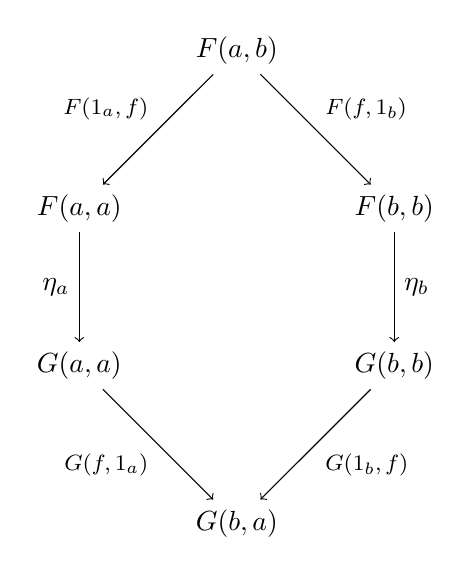
\begin{tikzpicture}
				\node (ab) at (0, 6) {$F(a, b)$};
				\node (F1) at (-2, 4) {$F(a, a)$};
				\node (F2) at (2, 4) {$F(b, b)$};
				\node (G1) at (-2, 2) {$G(a, a)$};
				\node (G2) at (2, 2) {$G(b, b)$};
				\node (ba) at (0, 0) {$G(b, a)$};
				
				\draw[->] (ab) edge node[above left]{\footnotesize$F(\mathbbm{1}_a, f)$} (F1) (F1) edge node[left]{$\eta_a$} (G1) (G1) edge node[below left]{\footnotesize$G(f, \mathbbm{1}_a)$} (ba);
				\draw[->] (ab) edge node[above right]{\footnotesize$F(f, \mathbbm{1}_b)$} (F2) (F2) edge node[right]{$\eta_b$} (G2) (G2) edge node[below right]{\footnotesize$G(\mathbbm{1}_b, f)$} (ba);
			\end{tikzpicture}
			\caption{Dinatural transformation.}
			\label{fig:dinatural}
		\end{figure}
	}
	
\subsection{Adjunctions}

	\newdef{Hom-set adjunction}{\index{adjunction}
		Let $\func{F}{C}{D}$ and $\func{G}{D}{C}$ be two functors. These functors form a hom-set adjunction (often just called an adjunction) if the following isomorphism is natural in $a, b$:
		\begin{gather}
			\text{hom}_D(Fa, b)\cong\text{hom}_C(a, Gb)
		\end{gather}
		The functor $F$ (resp. G) is called the left (resp. right) adjoint\footnote{Sometimes the word \textbf{adjunct} is used (French versus Latin).}.
	}
	\begin{notation}
		An adjunction$(F, G)$ between categories $\mathbf{C}, \mathbf{D}$ is often denoted by: \[\textbf{C}\adj{F}{G}\textbf{D}\] or if the ambient categories are clear by: \[F\dashv G\]
	\end{notation}
	
	\newdef{Unit-counit adjunction}{\index{triangle!identities}\index{unit}\index{zig-zag|see{triangle identity}}
		Let $\func{F}{C}{D}$ and $\func{G}{D}{C}$ be two functors. These functors form a unit-counit adjunction if there exist natural transformations
		\begin{align}
			\varepsilon: F\circ G\Rightarrow 1_D\\
			\eta: 1_C\Rightarrow G\circ F
		\end{align}
		such that the following compositions are identity morphisms:
		\begin{align}
			F\xrightarrow{F\eta}FGF\xrightarrow{\varepsilon F}F\\
			G\xrightarrow{\eta G}GFG\xrightarrow{G\varepsilon}G
		\end{align}
		These identities are sometimes called the \textbf{triangle identities} or \textbf{zig-zag identities} (the latter results from the shape of the associated string diagram). The transformations $\varepsilon$ and $\eta$ are called the \textbf{unit} and \textbf{counit} respectively.
	}
	
	\begin{property}
		Every hom-set adjuction induces a unit-counit adjunction. Let $\Phi_{a, b}$ be the natural isomorphism associated to the hom-set adjunction $F\dashv G$. The unit $\varepsilon_d$ is obtained as the adjunct $\Phi^{-1}_{Gd, d}(1_{Gd})$ of the identity morphism on $Gd\in\ob{C}$ and the counit $\eta_c$ is analogously defined as the adjunct $\Phi_{c, Fc}(1_{Fc})$ of the identity morphism at $Fc\in\ob{D}$.
		
		Similarly every unit-counit adjunction induces a hom-set adjunction. Consider a morphism $f:Fc\rightarrow d$. The (right) adjunct $\tilde{f}$ is defined as the composition \[Gf\circ\eta_c:c\rightarrow (G\circ F)c\rightarrow Gd\] Similarly, consider a morphism $\tilde{g}:c\rightarrow Gd$. The (left) adjunct $g$ is defined as the composition \[\varepsilon_d\circ F\tilde{g}: Fc\rightarrow (F\circ G)d\rightarrow d\]
	\end{property}

	Now it should be obvious that the above definition of a unit-counit adjunction can be generalized to general 2-categories:
	\newdef{Adjunction in 2-category}{\index{adjunction}
		Let \textbf{C} be a 2-category. An adjunction in \textbf{C} is a pair of 1-morphisms $F:a\rightarrow b$ and $G:b\rightarrow a$ together with 2-morphisms $\varepsilon:F\circ G\Rightarrow 1_b$ and $\eta:1_a\Rightarrow G\circ F$ that satisfy the zig-zag identities.
	}
	
	\begin{remark}[Duals and adjunctions]
		If one looks at the defining relations of duals in a rigid monoidal category one should see that these are in fact the same as the defining relations of the unit and counit of an adjunction. This is a consequence of the fact that a 2-category with a single object can be regarded as a (strict) monoidal category where the composition in the 2-category becomes the tensor product in the monoidal category. Similarly adjoint 1-morphisms in the 2-category become duals in the monoidal category.
	\end{remark}

\subsection{Constructions}

	\newdef{Discrete fibration}{\index{fibration}
		Let $\func{F}{A}{B}$ be a functor. $F$ is a discrete fibration if for every object $A\in\ob{A}$ and every morphism $f:B\rightarrow FA$ in $\textbf{B}$ there exists a unique morphism $g:C\rightarrow A$ in $\textbf{A}$ such that $F(g) = f$, where $B\in\ob{B}, C\in\ob{A}$.
	}

	\newdef{Dagger category\footnotemark}{\index{category!dagger}\index{involution}\label{cat:dagger_category}
		\footnotetext{Also called a \textbf{$\dag$-category}.}
		A category equipped with a contravariant endofunctor, i.e. a functor $\dag:\textbf{C}^{op}\rightarrow\textbf{C}$, such that:
		\begin{enumerate}
			\item $\forall C\in\ob{C}: \mathbbm{1}_C^\dag = \mathbbm{1}_C$
			\item $\dag\circ\dag = \mathbbm{1}_C$
		\end{enumerate}
		The second property says that $\dag$ is an \textbf{involutive} functor.
	}
	\remark{The concept of a dagger structure allows the usual definition of \textbf{unitary} and \textbf{self-adjoint} morphisms.}\index{unitary}
	\begin{property}
		The unitary morphisms in a dagger category form a groupoid\footnote{See definition \ref{cat:groupoid}.}.
	\end{property}
	
	\newdef{Comma category}{\index{category!comma}
		Let $\textbf{A}, \textbf{B}$ and $\textbf{C}$ be three categories and let $\func{F}{A}{C}$ and $\func{G}{B}{C}$ be two functors. The comma category $F\downarrow G$ is defined as follows:
		\begin{itemize}
			\item Objects are triples $(A, B, \gamma)$ where $A\in\ob{A}, B\in\ob{B}$ and $\gamma:FA\rightarrow GB\in\text{hom}(\textbf{C})$.
			\item Morphisms $(A, B, \gamma)\rightarrow(K, L, \sigma)$ are pairs $(f, g)$ where $f:A\rightarrow K\in\text{hom}(\textbf{A})$ and $g:B\rightarrow L\in\text{hom}(\textbf{B})$ such that $\sigma\circ F(f) = G(g)\circ\gamma$.
			\item Composition of morphisms is defined componentwise.
		\end{itemize}
	}
	\newdef{Slice category}{\index{category!slice}
		Let \textbf{C} be a category and let $c\in\ob{C}$. The slice category $\textbf{C}/c$ of $\textbf{C}$ over $c$ is defined as follows:
		\begin{itemize}
			\item The objects are morphisms in $\textbf{C}$ with codomain $c$.
			\item The morphisms $f\rightarrow g$ are morphisms $h$ in $\textbf{C}$ such that $g\circ h = f$.
		\end{itemize}
	}
	
\subsection{Monads}

	\newdef{Monad}{\index{monad}
		A monad is a triple $(T, \mu, \eta)$ where $\func{T}{C}{C}$ is an endofunctor and $\mu:T^2\rightarrow T, \eta:\text{id}_{\mathbf{C}}\rightarrow T$ are natural transformations satisfying the following (coherence) conditions:
		\begin{enumerate}
			\item As natural transformation from $T^3$ to $T$ we have:
			\begin{gather}
				\mu\circ T\mu = \mu\circ\mu_T
			\end{gather}
			\item As natural transformation from $T$ to itself we have:
			\begin{gather}
				\mu\circ T\eta = \mu\circ\eta_T = \mathbbm{1}
			\end{gather}
		\end{enumerate}
		These conditions say that a monad is a monoid in the category $\mathbf{End}_{\mathbf{C}}$ of endofunctors on $\mathbf{C}$.
	}
	\begin{example}[Adjunction]
		Every adjunction $F\dashv G$, with unit $\varepsilon$ and counit $\eta$, induces a monad of the form $(GF, G\varepsilon F, \eta)$.
	\end{example}
	
	\newdef{Algebra\footnotemark\ over a monad}{\index{algebra!over a monad}
		\footnotetext{A more suitable name would be ''module over a monad'', since these are modules over a monoid if we view monads as monoids in $\mathbf{End}_{\mathbf{C}}$.}
		Consider a monad $(T, \mu, \eta)$ on a category $\mathbf{C}$. A algebra over $T$ is a couple $(a, \kappa)$ where $a\in\ob{C}$ and $\kappa:Ta\rightarrow a$ such that the following conditions are satisfied:
		\begin{enumerate}
			\item $\kappa\circ T\kappa = \kappa\circ\mu_a$
			\item $\kappa\circ\eta_a = \mathbbm{1}_a$
		\end{enumerate}
		Morphisms $(a, \kappa_a)\rightarrow(b, \kappa_b)$ of $T$-algebras are morphisms $f:a\rightarrow b$ in $\mathbf{C}$ such that $f\circ\kappa_a = \kappa_b\circ Tf$.
	}
	\newdef{Eilenberg-Moore category}{\index{Eilenberg-Moore}
		Given a monad $T$ over a category $\mathbf{C}$ we define the Eilenberg-Moore category $\mathbf{C}^T$ as the category of $T$-algebras.
	}
	
	\newdef{Monadic adjunction}{
		An adjunction between categories $\mathbf{C}$ and $\mathbf{D}$ is said to be monadic if there exists an equivalence between $D$ and the Eilenberg-Moore category of the induced monad.
	}
	\newdef{Monadic functor}{\index{functor!monadic}
		A functor is said to be monadic if it admits a left adjoint such that the adjunction is monadic.
	}
	
	\begin{theorem}[Beck's monadicity theorem]
		Consider a functor $\func{F}{C}{D}$. This functor is monadic if and only if the following conditions are satisfied:
		\begin{itemize}
			\item $F$ admits a left adjoint.
			\item $F$ reflects isomorphisms.
			\item $\mathbf{C}$ has all coequalizers of $F$-split parallel pairs\footnote{These are parallel pairs $f,g$ such that the image $Ff, Fg$ under $F$ admits a split coequalizer.} and $F$ preserves these coequalizers.
		\end{itemize}
	\end{theorem}
	\remark{A sufficient condition for monadicity is obtained by replacing the third item above by the following weaker statement: ''$\mathbf{C}$ has all coequalizers of reflexive pairs and $F$ preserves these coequalizers.'' This weaker form is called the \textbf{crude monadicity theorem}.}

	\newdef{Closure operator\footnotemark}{\label{cat:closure_operator}\index{closure!operator}\index{modal operator|see{closure operator}}
		\footnotetext{Also called a \textbf{modal operator}.}
		Consider a monad $\func{T}{C}{C}$ with unit and product maps $\eta, \mu$. This monad is called a closure operator if the product map is a natural isomorphism.
		
		Given a closure operator $\func{T}{C}{C}$, one calls the object $Tx$ the closure of $x\in\ob{C}$. The \textbf{closing map} of an object $x\in\ob{C}$ is defined as the morphism $\eta_x$ and $x$ is said to be $T$\textbf{-closed} exactly if its closing map is an isomorphism.
	}

\section{Initial and terminal objects}

	\newdef{Initial object}{
		An object $O$ in a category $\textbf{C}$ is called initial if for every other object $P$ there exists a unique morphism $\iota_P:O\rightarrow P$.
	}
	\newdef{Terminal object}{
		An object $O$ in a category $\textbf{C}$ is called terminal if for every other object $P$ there exists a unique morphism $\tau_P:P\rightarrow O$. This object is sometimes denoted by $\mathbf{1}$.
	}
	\begin{property}
		If an initial (resp. terminal) object exists, then it is unique (possibly up to isomorphism).
	\end{property}
	\newdef{Well-pointed category}{
		A category is said to be well-pointed if the terminal object is a generator\footnote{See definition \ref{cat:generator}.}.
	}
	
	\newdef{Zero object}{\index{zero!object}\label{cat:zero_object}
		An object which is both initial and terminal. The zero object is often denoted by $\mathbf{0}$.
	}
	\begin{property}[Zero morphism]
		From the definition of the zero object it follows that for any two objects $A, B$ there exists a unique morphism $0_{AB}:A\rightarrow0\rightarrow B$.
	\end{property}
	\newdef{Pointed category}{\index{pointed!category}
		A category is said to be pointed if it contains a zero object.
	}
	
	\newdef{Global element}{\index{global!element}\label{category:global_element}
		Let $\textbf{C}$ be a category with terminal object $\mathbf{1}$. A global element of an object $X\in\ob{C}$ is a morphism $\mathbf{1}\rightarrow X$.
	}
	\begin{remark}
		In the category \textbf{Set} the elements of a set $S$ are in one-to-one correspondence with the global elements of $S$ and one has the important property (axiom) that two functions $f, g:S\rightarrow S'$ coincide if their evaluation at every element $s\in S$ is equal or equivalently if the precompositions with global elements coincide.
		
		However this way of checking equality can fail in other categories. Consider for example \textbf{Grp}. In this category the terminal object is $0 = \{e\}$. The only morphism from this group to any other group $G$ is the one mapping $e$ to the unit in $G$ ($0$ is also an initial object in \textbf{Grp}). It is obvious that precomposition with this morphism tells us nothing about the equality of other morphisms. To recover the technique used in \textbf{Set} one needs to generalize the notion of "element":
	\end{remark}
	\newdef{Generalized element}{\index{shape}
		Let $\textbf{C}$ be category and consider an object $X$ in $\textbf{C}$. For any object $Y\in\ob{C}$ one calls a morphism $Y\rightarrow X$ a generalized element of $X$. The morphisms $Y\rightarrow X$ are also called $\textbf{Y-elements}$ in $X$ or elements of \textbf{shape} $Y$ in $X$.
	}

\section{Diagrams and universal constructions}

	\newdef{Diagram}{\index{diagram}
		A diagram in $\textbf{C}$ with index category $\textbf{I}$ is a (covariant) functor $\func{D}{I}{C}$.
	}
	
	\newdef{Cone}{\index{cone}
		Let $\func{D}{I}{C}$ be a diagram. A cone from $a\in\ob{C}$ to $D$ consists of a family of morphisms $\psi_i:a\rightarrow Di, \forall i\in\ob{I}$ such that $\psi_j = Df\circ\psi_i$ for all morphisms $f:i\rightarrow j\in\text{hom}(\textbf{I})$, as depicted in figure \ref{fig:cone_component}.
		
		\begin{figure}[ht!]
			\centering
			\begin{subfigure}[b]{0.49\textwidth}
				\centering
				\begin{tikzpicture}
					\matrix (m) [matrix of math nodes,row sep=3em,column sep=3em, minimum width=1em, ampersand replacement=\&]{
						\&a\&\\
						Di\vphantom{(}\&\&Df(i)\\
					};
					\draw[->] (m-1-2) -- (m-2-1) node[pos=0.5, above left]{$\psi_i$};
					\draw[->] (m-1-2) -- (m-2-3) node[pos=0.5, above right]{$\psi_{f(i)}$};
					\draw[->] (m-2-1) -- (m-2-3) node[pos=0.5, below]{$Df$};
				\end{tikzpicture}
				\caption{Component of cone over $D$.}
				\label{fig:cone_component}
			\end{subfigure}
			\begin{subfigure}[b]{0.49\textwidth}
				\centering
				\begin{tikzpicture}
					\matrix (m) [matrix of math nodes,row sep=3em,column sep=3em, minimum width=1em, ampersand replacement=\&]{
						a\vphantom{b}\&\&b\\
						\&Di\&\\
					};
					\draw[->] (m-1-1) -- (m-2-2) node[pos=0.5, below left]{$\psi_i$};
					\draw[->] (m-1-3) -- (m-2-2) node[pos=0.5, below right]{$\phi_i$};
					\draw[->] (m-1-1) -- (m-1-3) node[pos=0.5, above]{$f$};
				\end{tikzpicture}
				\caption{Morphism of cones.}
				\label{fig:cone_morphism}
			\end{subfigure}
			\label{fig:cone}
		\end{figure}
	}
	\begin{adefinition}\index{diagonal!functor}
		This definition can be reformulated by defining an additional functor\footnote{The notation $\Delta_a$ tells us that $\Delta:C\rightarrow [\textbf{I},\textbf{C}]$ is the \textbf{diagonal functor}, i.e. $\Delta_c\equiv\Delta(c)$ is the constant functor from $\textbf{I}$ to $\textbf{C}$ with target object $c$.} $\Delta_a:\textbf{I}\rightarrow\textbf{C}$ which maps every element $i\in\ob{I}$ to $a$ and every morphism $g\in\text{hom}(\textbf{I})$ to id$_a$. The morphisms $\psi_c$ can then be seen as the components of a natural transformation $\psi:\Delta_a\Rightarrow D$. Hence a cone $(a, \psi)$ is an element of $[\textbf{I}, \textbf{C}](\Delta_a, D)$.
	\end{adefinition}

	\newdef{Morphism of cones}{\index{morphism!of cones}
		Let $\func{D}{I}{C}$ be a diagram and let $(a, \psi), (b, \phi)$ be cones to $D$. A morphism between these cones is a morphism of the apexes $f:a\rightarrow b$ such that the diagrams of the form \ref{fig:cone_morphism} commute for all $i\in\ob{I}$. The cones to $D$ together with these morphisms form a category $\textbf{Cone}(D)$, in fact this can easily be seen to be the comma category $(\Delta \downarrow D)$.
	}
	
	\newdef{Limit}{\index{limit}
		Consider a diagram $\func{D}{I}{C}$. The limit $\lim D$ of this diagram, if it exists, is the terminal object of the category $\textbf{Cone}(D)$.
	}
	This definition gives us the following universal property:
	\begin{uproperty}
		Let $\func{D}{I}{C}$ be a diagram and let $\lim D$ be its limit. For every cone $(a, \psi)\in\textbf{Cone}(D)$ there exists a unique morphism $f:c\rightarrow\lim D$.
	\end{uproperty}
	
	\begin{example}[Terminal object]
		A terminal object $\mathbf{1}$ is a limit over the empty diagram.
	\end{example}
	
	\newdef{Equalizer}{\index{equalizer}\index{fork}
		Consider the following diagram:\[X\overset{f}{\underset{g}{\rightrightarrows}} Y\] The limit of this diagram is called the equalizer of $f$ and $g$. Explicitly the equalizer is the universal object $E$ together with a morphism $e: E\rightarrow X$ such that $f\circ e = g\circ e$.
	}
	\newdef{Split coequalizer}{
		First we define a \textbf{cofork} diagram, i.e. a diagram \[a\overset{f}{\underset{g}{\rightrightarrows}} b\overset{t}{\rightarrow} c\] where $t\circ f = t\circ g$. A split coequalizer\footnote{A coequalizer, as obtained by dualizing the previous definition, is just a universal cofork.} is a cofork together with a section of $\varphi$ of $f$ and a section $\sigma$ of $t$ such that $\sigma\circ t = g\circ \varphi$.
	}
	
	\newdef{Finitely complete category}{\index{finitely!complete}
		A category is said to be finitely complete if it has a terminal object and if all binary equalizers and products exist.
	}
	\newadef{Finitely complete category}{
		A category is said to be finitely complete if all finite limits exist.
	}
	
	\newdef{Span}{\index{span}
		A span in a category $C$ is a diagram of the form \ref{fig:cat_span}.
		
		Let $\Lambda$ be the category with three objects $\{-1, 0, 1\}$ and two morphisms $i:0\rightarrow -1$ and $j:0\rightarrow 1$. By the above definition of a diagram a span in $C$ is equivalent to a functor $\func{S}{\Lambda}{C}$.
	}
	
	\newdef{Pullback\footnotemark}{\index{pullback}\label{cat:pullback}
		\footnotetext{Also called a \textbf{fibre product} or \textbf{Cartesian square}.}
		The pullback of two morphisms $f:A\rightarrow C$ and $g:B\rightarrow C$ is defined as the limit of cospan \ref{fig:pullback}.
	}
	\begin{figure}[!ht]
		\centering
		\begin{subfigure}[b]{0.49\textwidth}
			\centering
			\begin{tikzpicture}
				\matrix (m) [matrix of math nodes,row sep=2em,column sep=2em, minimum width=1em, ampersand replacement=\&]{
					\&S\&\\
					A\&\&B\\
				};
				\draw[->] (m-1-2) -- (m-2-1) node[pos=0.5, above left]{$f$};
				\draw[->] (m-1-2) -- (m-2-3) node[pos=0.5, above right]{$g$};
			\end{tikzpicture}
			\caption{Span (category theory).}
			\label{fig:cat_span}
		\end{subfigure}
		\begin{subfigure}[b]{0.49\textwidth}
			\centering
			\begin{tikzpicture}
				\matrix (m) [matrix of math nodes,row sep=2em,column sep=2em, minimum width=1em, ampersand replacement=\&]{
					A\&\&B\\
					\&C\&\\
				};
				\draw[->] (m-1-1) -- (m-2-2) node[pos=0.5, below left]{$f$};
				\draw[->] (m-1-3) -- (m-2-2) node[pos=0.5, below right]{$g$};
			\end{tikzpicture}
			\caption{Cospan.}
			\label{fig:pullback}
		\end{subfigure}
		\caption{}
	\end{figure}
	
	\begin{notation}[Pullback]
		The pullback of two morphisms $f:A\rightarrow C$ and $g:B\rightarrow C$ is often denoted by $A\times_C B$.
	\end{notation}
	
	\begin{property}
		If a terminal object $\mathbf{1}$ exists then the pullback $A\times_{\mathbf{1}}B$ is equal to the (Cartesian) product  $A\times B$.
	\end{property}
	\newdef{Pushout}{\index{pushout}
		The dual notion of a pullback, i.e. the colimit of a span.
	}

	\newdef{Wedge}{\index{wedge}
		Consider a profunctor $F:\mathbf{C}^{op}\times\mathbf{C}\rightarrow\mathbf{Set}$. A wedge $e:w\rightarrow F$ is an object $w\in\ob{Set}$ together with a collection of morphisms $e_c:w\rightarrow F(c, c)$ indexed by $\ob{C}$ such that for any morphism $f:c\rightarrow c'$ the following diagram commutes:
		\begin{gather*}
			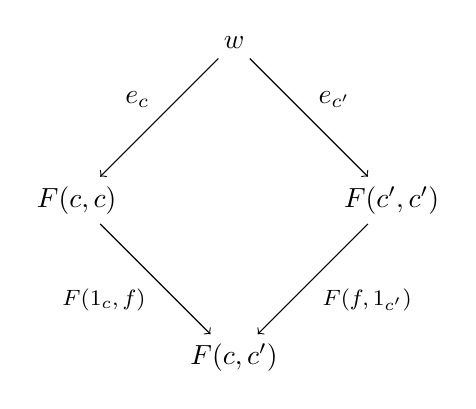
\begin{tikzpicture}
				\node (W) at (0, 4) {$w$};
				\node (F1) at (-2, 2) {$F(c, c)$};
				\node (F2) at (2, 2) {$F(c', c')$};
				\node (F) at (0, 0) {$F(c, c')$};
				\draw[->] (W) edge node[above left]{$e_c$} (F1) (F1) edge node[below left]{\footnotesize$F(\mathbbm{1}_c, f)$} (F);
				\draw[->] (W) edge node[above right]{$e_{c'}$} (F2) (F2) edge node[below right]{\footnotesize$F(f, \mathbbm{1}_{c'})$} (F);
			\end{tikzpicture}
		\end{gather*}
		As was the case for cones, one can reformulate this in terms of (di)natural transformations. A wedge $(w, e)$ of a profunctor $F:\mathbf{C}^{op}\times\mathbf{C}\rightarrow\mathbf{Set}$ is a dinatural transformation from the constant profunctor $\Delta_w$ to $F$.
	}
	\newdef{End}{\index{end}
		The end of a profunctor $F:\mathbf{C}^{op}\times\mathbf{C}\rightarrow\mathbf{Set}$ is defined as the universal wedge of $F$. The components of the wedge are called the \textbf{projection maps} of the end. This stems from the fact that for a discrete category the end coincides with the product $\prod_{c\in\ob{C}}F(c, c)$.
	}
	\newnot{End}{
		The end of a profunctor $F:\mathbf{C}^{op}\times\mathbf{C}\rightarrow\mathbf{Set}$ is often denoted using an integral sign with subscript: \[\int_{c\in\mathbf{C}}F(c, c)\] For the dual construction, i.e. a \textbf{coend}, one uses the integral sign with superscript.
	}
	\begin{example}[Natural transformations]
		Consider two functors $\func{F, G}{C}{D}$. The map $(c, c')\mapsto\mathbf{D}(Fc, Gc')$ gives a profunctor $H:\mathbf{C}^{op}\times\mathbf{C}\rightarrow\mathbf{Set}$. If we look at the wedge condition for this profunctor (especially the lower half) we get the following equality for all morphisms $f:c\rightarrow c'$:
		\begin{gather}
			\tau_{c'}\circ Ff = Gf\circ \tau_c
		\end{gather}
		where $\tau_c$ is the projection of the wedge associated to the object $c\in\ob{C}$. Comparing this equality to definition \ref{cat:natural} we immediately see that the end $\int_{c\in\mathbf{C}}\mathbf{D}(Fc, Gc)$ is exactly Nat$(F, G)$.
	\end{example}
	
	\begin{property}
		The following equality can be used to turn ends into coends and vice versa:
		\begin{gather}
			\mathbf{Set}\left(\int^{c\in\mathbf{C}}F(c, c), c'\right) = \int_{c\in\mathbf{C}}\mathbf{Set}\left(F(c, c), c'\right)
		\end{gather}
	\end{property}
	
	Using the above properties and definitions one obtains the following Yoneda-like statements:
	\begin{theorem}[Ninja Yoneda lemma]\index{Yoneda!lemma}
		Let $\func{F}{C}{D}$ be a covariant functor. The following two isomorphisms follow from the ordinary Yoneda lemma:
		\begin{gather}
			\int_{c'\in\mathbf{C}}\mathbf{Set}\left(\mathbf{C}(c, c'), Fc'\right)\cong Fc
		\end{gather}
		\begin{gather}
			\int^{c\in\mathbf{C}}\mathbf{C}(c, c')\times Fc\cong Fc'
		\end{gather}
	\end{theorem}
	
	\newdef{Kan extension}{\index{Kan!extension}
		Consider two functors $\func{F}{C}{D}$ and $\func{G}{C}{E}$ and denote the terminal category by $\mathbf{1}$. The right Kan extension\footnote{The left Kan extension Lan$_GF$ is obtained by dualizing this construction.} of $F$ along $G$ is given by the universal functor $\func{\text{Ran}_GF}{E}{D}$ and natural transformation $\eta:\text{Ran}_GF\circ G\Rightarrow F$:
		\begin{gather*}
			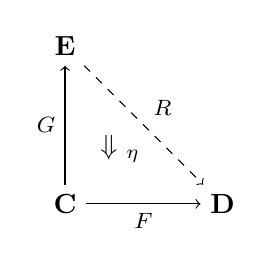
\begin{tikzpicture}
				\node (E) at (0, 2) {$\mathbf{E}$};
				\node (C) at (0, 0) {$\mathbf{C}$};
				\node (D) at (2, 0) {$\mathbf{D}$};
				\node (A) at (0.7, 0.7) {$\Downarrow_{\ \eta}$};
				\draw[->] (C) -- node[left]{\footnotesize$G$} (E);
				\draw[->] (C) -- node[below]{\footnotesize$F$} (D);
				\draw[dashed, ->] (E) -- node[above right]{\footnotesize$R$} (D);
			\end{tikzpicture}
		\end{gather*}
		Universality means that every other natural transformation $\chi:H\circ G\Rightarrow F$ factors uniquely through $\eta$.
	}
	\begin{example}[Limit]
		By choosing the functor $G$ in the definition of a right Kan extension to be the unique functor $!_C:\mathbf{C}\rightarrow\mathbf{1}$ into the terminal category one obtains the definition of a limit, i.e. $\lim F = \text{Ran}_{!_C}F$. Similarly one can obtain the colimit as the left Kan extension.
	\end{example}
	
	\newdef{Absolute Kan extension}{
		A (left) Kan extension Lan$_GF$ is said to be absolute if for every functor $H$ with the same codomain as $F$ the following isomorphism holds:
		\begin{gather}
			H(\text{Lan}_GF)\cong\text{Lan}_G(HF)
		\end{gather}
		There exists an analogous definition for right Kan extensions.
	}

	\newadef{Kan extension}{
		The construction above gives a functor Ran$_G$ from the functor category $[\mathbf{C}, \mathbf{D}]$ to the functor category $[\mathbf{E}, \mathbf{D}]$. The right Kan extension Ran$_G$ can be defined as the right adjoint to the pullback functor $G^*:F\mapsto F\circ G$. Similarly one can define the left Kan extension as the left adjoint to the pullback functor $G^*$.
	}
	\remark{Using this equivalence of hom-spaces one can generalize the Kan extension from $\mathbf{Cat}$ to any 2-category.}
	
	The existence of Kan extensions can also be used to determine the existence of adjoints:
	\begin{property}
		A functor $\func{F}{C}{D}$ admits a left adjoint\footnote{An analogous statement holds for right adjoints.} if and only if the right Kan extension of the identity functor $\func{\mathbbm{1}}{C}{C}$ along $F$ exists. If it exists and if it is an absolute extension then the left adjoint is given exactly by this Kan extension.
	\end{property}
	
\section{Morphisms}

	\newdef{Section}{\index{section}
		A section of a morphism $f:a\rightarrow b$ is a right-inverse, i.e. a morphism $g:b\rightarrow a$ such that $f\circ g=\mathbbm{1}_b$.
	}
	\newdef{Monomorphism}{\index{monomorphism}
		Let \textbf{C} be a category. A morphism $\mu\in\textbf{C}(A, B)$ is called a mono\footnote{Sometimes just a \textbf{mono} or a \textbf{monic} morphism.} if for every object $X\in\ob{C}$ and every two morphisms $\alpha_1, \alpha_2\in\textbf{C}(X, A)$ such that $\mu\circ\alpha_1 = \mu\circ\alpha_2$ we can conclude that $\alpha_1=\alpha_2$.
	}
	\newdef{Epimorphism}{\index{epimorphism}
		Let \textbf{C} be a category. A morphism $\varepsilon\in\textbf{C}(A, B)$ is called an epimorphism\footnote{Sometimes just an \textbf{epi} or an \textbf{epic} morphism.} if for every object $X\in\ob{C}$ and every two morphisms $\alpha_1, \alpha_2\in\textbf{C}(B, X)$ such that $\alpha_1\circ\varepsilon = \alpha_2\circ\varepsilon$ we can conclude that $\alpha_1=\alpha_2$.
	}
	
	\newdef{Balanced category}{\index{category!balanced}\label{category:balanced}
		A category is said to be balanced if every monic epi is an isomorphism.
	}
	
	\begin{property}[Global elements]
		Every global element\footnote{See definition \ref{category:global_element}.} is monic.
	\end{property}
	
	\newdef{Reflexive pair}{
		Two parallel morphisms $f, g:a\rightarrow b$ are said to form a reflexive pair if they have a common section, i.e. there exists a morphism $\sigma:b\rightarrow a$ such that $f\circ\sigma=g\circ\sigma$.
	}
	
	\begin{property}[Equalizing morphism]
		Consider an equalizer $(E, e)$. The equalizing morphism $e$ is monic. Similarly a coequalizing morphism is epic.
	\end{property}

	\newdef{Regular monomorphism}{\index{regular!morphism}
		A mono is said to be regular if it arises as an equalizer of two parallel morphisms.
	}
	\begin{property}[Regular bimorphism]\label{category:regular_iso}
		A monic regular epimorphism is an isomorphism. Analogously so is an epic regular monomorphism is an isomorphism.
	\end{property}
	
	\newdef{Injective object}{\index{injective!object}
		Let \textbf{C} be an category. An object $I\in\ob{C}$ is said to be injective if for every $A, B\in\ob{C}$, mono $f:A\rightarrow B$ and morphism $g:A\rightarrow I$ there exists a morphism $\phi:B\rightarrow I$ such that $\phi\circ f = g$.
		\begin{figure}[ht!]
			\centering
			\begin{subfigure}[b]{0.49\textwidth}
				\centering
				\begin{tikzpicture}
					\matrix (m) [matrix of math nodes,row sep=7em,column sep=7em, minimum width=2em, ampersand replacement=\&]{
						A\&B\\
						I\&\\
					};
					\draw[right hook ->] (m-1-1) -- (m-1-2) node[pos=0.5, above]{$f$};
					\draw[->] (m-1-1) -- (m-2-1) node[pos=0.5, left]{$g$};
					\draw[dashed, ->] (m-1-2) -- (m-2-1) node[pos=0.5, below right]{$\phi$};
				\end{tikzpicture}
				\caption{Injective object $I$.}
				\label{fig:injective_object}
			\end{subfigure}
			\begin{subfigure}[b]{0.49\textwidth}
				\centering
				\begin{tikzpicture}
					\matrix (m) [matrix of math nodes,row sep=7em,column sep=7em, minimum width=2em, ampersand replacement=\&]{
						A\&B\\
						\&P\\
					};
					\draw[->>] (m-1-1) -- (m-1-2) node[pos=0.5, above]{$f$};
					\draw[->] (m-2-2) -- (m-1-2) node[pos=0.5, right]{$g$};
					\draw[dashed, ->] (m-2-2) -- (m-1-1) node[pos=0.5, below left]{$\phi$};
				\end{tikzpicture}
				\caption{Projective object $P$.}
				\label{fig:projective_object}
			\end{subfigure}
		\end{figure}
	}
	
	Dually one can construct:
	\newdef{Projective object}{\index{projective!object}
		Let \textbf{C} be an category. An object $P\in\ob{C}$ is said to be projective if for every $A, B\in\ob{C}$, epi $f:A\rightarrow B$ and morphism $g:P\rightarrow A$ there exists a morphism $\phi:P\rightarrow B$ such that $f\circ\phi = g$.
	}
	
	\newdef{Subobject}{\index{subobject}
		Let \textbf{C} be a category and let $A\in\ob{C}$ be any object. A subobject $B$ of $A$ is a mono $B\hookrightarrow A$.
		
		In fact one should work up to isomorphism and hence the complete definition goes as follows. A subobject $B$ of $A$ in the category \textbf{C} is an isomorphism class of monos $i:B\hookrightarrow A$ in the slice category $\textbf{C}/A$.
	}
	\newdef{Well-powered category}{\index{category!well-powered}
		A category \textbf{C} is said to be well-powered if for every object $A\in\ob{C}$ the class of subobjects \textbf{Sub}$(A)$ is small.
	}
	
	\newdef{Generator\footnotemark}{\index{generator}\label{cat:generator}
		\footnotetext{Also called a \textbf{separator}.}
		Let \textbf{C} be a category. A collection of objects $\{O_i\in\ob{C}\}$ is called a collection of generators for \textbf{C} if, given any two objects $A, B\in\ob{C}$ and any two morphisms $f, g:A\rightarrow B$, we have that $f\neq g\implies\exists j\in I, h_j\in\textbf{C}(O_i, A): f\circ h_j\neq g\circ h_j$.
	}
	
	\newdef{Decategorification}{
		Let \textbf{C} be a (essentially) small category. The set of isomorphism classes of \textbf{C} is called the decategorification of \textbf{C}. This is given by a functor \[K:\textbf{Cat}\rightarrow\textbf{Set}\]
	}
	
	\newdef{Lift}{\index{lift}
		A lift of a morphism $f:A\rightarrow B$ along an epi $e:X\rightarrow B$ is a morphisms $\tilde{f}:A\rightarrow X$ satisfying $f = e\circ\tilde{f}$.
	}
	\newdef{Lifting property}{\index{orthogonal}
		A morphism $f:A\rightarrow B$ has the left lifting property with respect to a morphism $g:C\rightarrow D$ if for every commutative diagram
		\begin{figure}[ht!]
			\centering
			\begin{tikzcd}[ampersand replacement=\&, row sep=4em,column sep=4em, minimum width=2em]
				A \arrow[r] \arrow[d, "f"'] \& C \arrow[d, "g"]\\
				B \arrow[ur, "\psi"] \arrow[r] \& D
			\end{tikzcd}
			\caption{Left lifting property.}
			\label{fig:lifting_property}
		\end{figure}
		there exists a morphism $\psi:B\rightarrow C$ such that the triangles commute. The morphism $g$ is also said to have the right lifting property with respect to $f$. If the morphism $\psi$ is unique then $f$ and $g$ are said to be \textbf{orthogonal}.
	}
	
	\newdef{Weak factorization system}{\index{weak!factorization}\label{category:wfc}
		Consider a category \textbf{C}. A pair $(L, R)$ of classes of morphisms in \textbf{C} is called a weak factorization system (WFS) if it satisfies the folllowing 3 properties:
		\begin{enumerate}
			\item Every morphism in \textbf{C} factors as a composition $g\circ f$ where $f\in L$ and $g\in R$.
			\item $L$ consists of the morphisms in \textbf{C} that have the left lifting property with respect to morphisms in $R$.
			\item $R$ consists of the morphisms in \textbf{C} that have the right lifting property with respect to morphisms in $L$.
		\end{enumerate}
	}
	
	\newdef{Localization}{\index{localization}\label{cat:localization}
		Consider a category \textbf{C} with a collection of morphism $M\subset\text{mor}(\textbf{C})$. The localization of \textbf{C} with respect to $M$ is constructed by adding for each morphism $f\in M$ a formal inverse to $\text{mor}(\textbf{C})$.
	}

\section{Abelian categories}

	\newdef{Pre-additive category}{
		A (locally small) category enriched over \textbf{Ab}, i.e. every hom-set is an Abelian group and composition is bilinear.
	}
	\newdef{$k$-linear category}{\index{category!linear}
		Let \textbf{Vect}$_k$ denote the category of vector spaces over the base field $k$. A $k$-linear category is a category enriched over \textbf{Vect}$_k$.
	}
	
	\begin{property}\index{zero!object}
		Let \textbf{A} be a pre-additive category and let $X\in\ob{A}$. The following statements are equivalent:
		\begin{itemize}
			\item $X$ is an initial object.
			\item $X$ is a final object.
			\item $\mathbbm{1}_X$ = 0
		\end{itemize}
		Any initial/terminal object is hence a zero object\footnote{See definition \ref{cat:zero_object}.}.
	\end{property}
	\begin{property}\index{biproduct}
		In a pre-additive category the finite products $\prod_{i\in I}X_i$ are isomorphic to the finite coproducts $\bigsqcup_{i\in I} X_i$ (which are called \textbf{direct sums} in this context). If a product $X\times Y$ exists then so does the coproduct $X\sqcup Y$ and if the coproduct exists then so does the product. In general if a product and coproduct exist and are equal then one speaks of a \textbf{biproduct}.
	\end{property}
	
	\newdef{Additive category}{\index{additive!category}
		A pre-additive category in which all finite biproducts exist.
	}
	
	If one speaks of additive categories, one generally assumes that the associated functors are of a specific type:
	\newdef{Additive functor}{\index{additive!functor}\label{additive_functor}
		Let $\mathbf{A}, \mathbf{A'}$ be additive categories. A functor $\func{F}{A}{A'}$ is said to be additive if it preserves all biproducts, i.e. if it satisfies the following conditions:
		\begin{itemize}
			\item It preserves zero objects: $F0_A \cong 0_{A'}$.
			\item There exists a natural isomorphism $F(X\oplus Y)\cong FX\oplus FY$.
		\end{itemize}
		
		One can generalize this notion to pre-additive categories. A functor between pre-additive categories is said to be additive if it acts as a group morphism on hom-spaces.
	}
	
	In a pre-additive category one can define the classical notions from (homological) algebra such as images and kernels:
	\newdef{Kernel}{\index{kernel}
		Let $f:X\rightarrow Y$ be a morphism. A\footnote{Note the word \textit{a}. The kernel of a morphism is determined up to an isomoprhism.} kernel is a morphism $k:Z\rightarrow X$ such that:
		\begin{itemize}
			\item $f\circ k = 0$
			\item Universal property: for every other morphism $k':Z'\rightarrow X$ such that $f\circ k' = 0$ there exists a unique morphism $h:Z'\rightarrow Z$ such that $k\circ h = k'$.
		\end{itemize}
		Hence a kernel of $f$ is an equalizer of $f$ and 0.
	}
	\begin{notation}[Kernel]
		If the kernel of $f:X\rightarrow Y$ exists then it is denoted by $\ker(f)\rightarrow X$.
	\end{notation}
	
	\newdef{Cokernel}{
		Let $f:X\rightarrow Y$ be a morphism. A cokernel is a morphism $p:Y\rightarrow Z$ such that:
		\begin{itemize}
			\item $p\circ f = 0$
			\item Universal property: for every other morphism $p':Y\rightarrow Z'$ such that $p'\circ f = 0$ there exists a unique morphism $h:Z\rightarrow Z'$ such that $h\circ p = p'$.
		\end{itemize}
		Hence a cokernel of $f$ is a coequalizer of $f$ and 0.
	}
	\begin{notation}[Cokernel]
		If the cokernel of $f:X\rightarrow Y$ exists then it is denoted by $Y\rightarrow\text{coker}(f)$.
	\end{notation}
	\remark{The name and notation of the kernel\footnote{Similarly for the cokernel.} (in the categorical sense) is explained by remarking that by Yoneda's lemma the morphism \[\ker(f)\rightarrow X\] represents the functor \[F:Z\mapsto\ker\Big(\textbf{C}(Z, X)\rightarrow\textbf{C}(Z, Y)\Big)\]}

	\newdef{Pre-Abelian category}{
		An additive category is pre-Abelian if every morphism has a kernel and cokernel.
	}
	\newdef{Abelian category}{\index{Abelian!category}
		A pre-Abelian category in which every mono is a kernel and every epi is a cokernel or equivalently if for every morphism $f$ there exists an isomorphism $\text{coker}(\ker(f))\cong\ker(\text{coker}(f))$.
	}
	
	\begin{property}
		In Abelian categories a morphism is monic if and only if it is injective, i.e. its kernel is 0. Analogously a morphism is epic if and only if it is surjective, i.e. its cokernel is 0.
	\end{property}

	\newdef{Exact functor}{\index{exact!functor}
		Let $\func{F}{A}{A'}$ be an additive functor between additive categories. We use the following definitions:
		\begin{itemize}
			\item $F$ is said to be left exact if it preserves kernels.
			\item $F$ is said to be right exact if it preserves cokernels.
			\item $F$ is said to be exact if it is both left and right exact.
		\end{itemize}
	}
	\begin{result}
		The previous definition implies the following properties (which can in fact be used as an alternative definition):
		\begin{itemize}
			\item If $F$ is left exact it maps an exact sequence of the form \[0\longrightarrow A\longrightarrow B\longrightarrow C\]
			to an exact sequence of the form \[0\longrightarrow FA\longrightarrow FB\longrightarrow FC\]
			\item If $F$ is right exact it maps an exact sequence of the form \[A\longrightarrow B\longrightarrow C\longrightarrow 0\]
			to an exact sequence of the form \[FA\longrightarrow FB\longrightarrow FC\longrightarrow 0\]
			\item If $F$ is exact it maps short exact sequences to short exact sequences.
		\end{itemize}
	\end{result}

\subsection{Size conditions}

	\newdef{Simple object}{\index{simple!object}
		Let \textbf{C} be an Abelian category. An object $A\in\ob{C}$ is said to be simple if the only subobjects of $A$ are $\mathbf{0}$ and $A$ itself. An object is said to be semisimple if it is a direct sum of simple obejcts.
	}
	\newdef{Semisimple category}{
		A category is said to be semisimple if every object is semisimple (where generally the direct sums are taken over finite index sets).
	}
	
	\newdef{Jordan-H\"older series}{\index{Jordan-H\"older}\index{finite}
		A filtration \[0\rightarrow X_1\rightarrow X_2\rightarrow\cdots\rightarrow X_n=X\] of an object $X$ is said to be a Jordan-H\"older series if the quotient objects $X_i/X_{i-1}$ are simple for all $i\leq n$. If the series is finite, i.e. $n\in\mathbb{N}$, then the object $X$ is said to be \textbf{finite}.
	}
	\begin{theorem}[Jordan-H\"older]
		If an object $X$ in an Abelian category is finite then every Jordan-H\"older series has the same length. In particular, the multiplicities of simple objects are the same for all such series.
	\end{theorem}
	\begin{theorem}[Krull-Schmidt]\index{Krull-Schmidt}\index{indecomposable}
		Any object in an Abelian category of finite length admits a unique decomposition as a direct sum of indecomposable\footnote{An object is \textbf{indecomposable} if it cannot be written as a direct sum of its subobjects.} objects.
	\end{theorem}
	
	\newdef{Locally finite}{\label{category:locally_finite}
		A $k$-linear Abelian category is said to be locally finite if it satisfies the following conditions:
		\begin{enumerate}
			\item Every hom-space is finite-dimensional.
			\item Every object has finite length.
		\end{enumerate}
	}
	\newdef{Finite}{\index{finite}
		A $k$-linear Abelian category is said to be finite if it satisfies the following conditions:
		\begin{enumerate}
			\item It is locally finite.
			\item It has enough projectives (or equivalently every simple object has a projective cover).
			\item The set of isomorphism classes of simple objects is finite.
		\end{enumerate}
	}
	
	\begin{theorem}[Schur's lemma]\index{Schur's lemma}
		Let $\mathbf{C}$ be an Abelian category. For every two simple objects $X, Y$ one has that every non-zero moprhism $X\rightarrow Y$ is an isomorphism. In particular, if $X, Y$ are two non-isomorphic simple objects then $\mathbf{C}(X, Y)=0$ and $\mathbf{C}(X, X)$ is a division algebra.
	\end{theorem}
	\begin{result}
		If $\mathbf{C}$ is locally finite and $k$ is algebraically closed then $\mathbf{C}(X, X)\cong k$ for all simple objects $X$.
	\end{result}

\section{Monoidal categories}

	\newdef{Monoidal category}{\index{monoidal!category}\index{tensor!product}\label{category:monoidal_category}
		A category \textbf{C} equipped with a bifunctor \[-\otimes -:\textbf{C}\times\textbf{C}\rightarrow\textbf{C}\] called the \textbf{tensor product} or \textbf{monoidal product}, together with a distinct object $\mathbf{1}$, called the \textbf{unit object}, and 3 natural isomorphisms, called the \textbf{coherence maps}:
		\begin{itemize}
			\item \textbf{Associator}: $\alpha_{A, B, C}:(A\otimes B)\otimes C\cong A\otimes(B\otimes C)$
			\item \textbf{Left unitor}: $\lambda_A:\mathbf{1}\otimes A\cong A$
			\item \textbf{Right unitor}: $\rho_A: A\otimes\mathbf{1}\cong A$
		\end{itemize}
		such that the \textbf{triangle} and \textbf{pentagon} diagrams commute. (See figures \ref{fig:triangle_diagram} and \ref{fig:pentagon_diagram}.)
		
		\begin{figure}[ht!]
			\centering
			\begin{tikzpicture}
				\matrix (m) [matrix of math nodes,row sep=4em,column sep=4em,minimum width=2em, ampersand replacement=\&]{
					(A\otimes\mathbf{1})\otimes B\&\&A\otimes(\mathbf{1}\otimes B)\\
					\&A\otimes B\&\\
				};
				
				\draw[->] (m-1-1) -- (m-1-3) node[pos=0.5, above]{$\alpha_{A, \mathbf{1}, B}$};
				\draw[->] (m-1-1) -- (m-2-2) node[pos=0.5, below left]{$\rho_A\otimes\mathbbm{1}$};
				\draw[->] (m-1-3) -- (m-2-2) node[pos=0.5, below right]{$\mathbbm{1}\otimes\lambda_B$};
			\end{tikzpicture}
			\caption{Triangle diagram.}
			\label{fig:triangle_diagram}
		\end{figure}
		\begin{figure}[ht!]
			\centering
			\begin{tikzpicture}
				\matrix (m) [matrix of math nodes,row sep=4em,column sep=-2em,minimum width=1em, ampersand replacement=\&]{
					\&((A\otimes B)\otimes C)\otimes D\&\&(A\otimes (B\otimes C))\otimes D\&\\
					(A\otimes B)\otimes(C\otimes D)\&\&\&\&A\otimes((B\otimes C)\otimes D)\\
					\&\&A\otimes(B\otimes (C\otimes D))\&\&\\
				};
				
				\draw[->] (m-1-2) -- (m-1-4) node[pos=0.5, above]{$\alpha_{A, B, C}\otimes\mathbbm{1}$};
				\draw[->] (m-1-2) -- (m-2-1) node[pos=0.5, above left]{$\alpha_{A\otimes B, C, D}$};
				\draw[->] (m-2-1) -- (m-3-3) node[pos=0.5, below left]{$\alpha_{A, B, C\otimes D}$};
				\draw[->] (m-1-4) -- (m-2-5) node[pos=0.5, above right]{$\alpha_{A, B\otimes C, D}$};
				\draw[->] (m-2-5) -- (m-3-3) node[pos=0.5, below right]{$\mathbbm{1}\otimes\alpha_{B, C, D}$};
			\end{tikzpicture}
			\caption{Pentagon diagram.}
			\label{fig:pentagon_diagram}
		\end{figure}
	}
	
	\newdef{Strict monoidal category}{
		A monoidal category is called strict if the associator $\alpha$ and the unitors $\lambda,\rho$ are identity morphisms.
	}
	
	\newdef{Scalar}{\index{scalar}
		In a monoidal category the scalars are defined as the endomorphisms $\mathbf{1}\rightarrow\mathbf{1}$.
	}
	\begin{property}
		The set of scalars forms a commutative monoid.
	\end{property}
	\begin{property}
		Every scalar $s:\mathbf{1}\rightarrow\mathbf{1}$ induces a natural transformation \[s_A:A\cong\mathbf{1}\otimes A\xrightarrow{s\otimes\mathbbm{1}}\mathbf{1}\otimes A\cong A\] satisfying the "usual" rules of scalar multiplication in linear algebra:
		\begin{itemize}
			\item $s\diamond(s'\diamond f) = (s\circ s')\diamond f$
			\item $(s\diamond f)\circ(s'\diamond g) = (s\circ s')\diamond(f\circ g)$
			\item $(s\diamond f)\otimes(s'\diamond g) = (s\circ s')\diamond(f\otimes g)$
		\end{itemize}
		where $s\diamond f$ denotes $f\circ s_A = s_B\circ f$.
	\end{property}
	
	\newdef{Weak inverse}{\index{weak!inverse}
		Let $(\textbf{C},\otimes, \mathbf{1})$ be a monoidal category. Consider an object $X\in\ob{C}$. An object $Y\in\ob{C}$ is called a weak inverse of $X$ if it satisfies $X\otimes Y\cong\mathbf{1}$.
	}
	\remark{One can show that the existence of a one-sided weak inverse (as in the definition above) is sufficient to prove that it is in fact a two-sided weak inverse, i.e. $Y\otimes X\cong\mathbf{1}$.}
	
	\begin{theorem}[MacLane's coherence theorem]\index{coherence!theorem}
		Let $\textbf{C}, \textbf{D}$ be monoidal categories. Any two natural transformations $\eta, \varepsilon:F\Rightarrow G$ constructed solely from the associator $\alpha$ and the unitors $\lambda,\rho$ coincide.
	\end{theorem}
	
	\newdef{Closed monoidal category}{
		A monoidal category $(\textbf{C}, \otimes, \mathbf{1})$ is said to be closed monoidal if for every object $B\in\ob{C}$ there exists a a right adjoint\footnote{See definition \ref{category:internal_hom} of an \textit{internal hom} for more information.} to the tensor product functor $-\otimes B:\textbf{C}\rightarrow\textbf{C}$, i.e.:
		\begin{gather}
			\forall A, C\in\ob{C}:\exists B\Rightarrow C\in\ob{C}:\textbf{C}(A\otimes B, C)\cong\textbf{C}(A, B\Rightarrow C)
		\end{gather}
		where the isomorphism is natural in $A, C\in\ob{C}$.
	}
	
\subsection{Monoidal functors}
	
	\newdef{Monoidal functor}{\index{monoidal!functor}\index{coherence!maps}
		Let $(\textbf{C}, \otimes, \mathbf{1}_C), (\textbf{D}, \circledast, \mathbf{1}_D)$ be two monoidal categories. A functor $\func{F}{C}{D}$ is said to be monoidal if there exists:
		\begin{itemize}
			\item A natural isomorphism $\psi_{A, B}: FA\circledast FB\Rightarrow F(A\otimes B)$ such that the diagram in figure \ref{fig:monoidal_functor1} commutes.
			\begin{figure}[ht!]
				\centering
				\begin{tikzpicture}
					\matrix (m) [matrix of math nodes,row sep=4em,column sep=4em, minimum width=1em, ampersand replacement=\&]{
						(FA\circledast FB)\circledast FC\&FA\circledast(FB\circledast FC)\\
						F(A\otimes B)\circledast FC\&FA\circledast F(B\otimes C)\\
						F\Big((A\otimes B)\otimes C\Big)\&F\Big(A\otimes (B\otimes C)\Big)\\
					};
					\draw[->] (m-1-1) -- (m-1-2) node[pos=0.5, above]{$\alpha_{\textbf{D}}$};
					\draw[->] (m-3-1) -- (m-3-2) node[pos=0.5, below]{$F(\alpha_{\textbf{C}})$};
					
					\draw[->] (m-1-1) -- (m-2-1) node[pos=0.5, left]{$\psi_{A, B}\circledast\mathbbm{1}$};
					\draw[->] (m-2-1) -- (m-3-1) node[pos=0.5, left]{$\psi_{A\otimes B, C}$};
					\draw[->] (m-1-2) -- (m-2-2) node[pos=0.5, right]{$\mathbbm{1}\circledast\psi_{B, C}$};
					\draw[->] (m-2-2) -- (m-3-2) node[pos=0.5, right]{$\psi_{A, B\otimes C}$};
				\end{tikzpicture}
				\caption{}
				\label{fig:monoidal_functor1}
			\end{figure}

			\item An isomorphism $\phi: \mathbf{1}_D\rightarrow F\mathbf{1}_C$ which makes the two diagrams in figure \ref{fig:unitality} commute.
		\begin{figure}[ht!]
			\centering
			\begin{subfigure}[b]{0.49\textwidth}
				\centering
				\begin{tikzpicture}
					\matrix (m) [matrix of math nodes,row sep=4em,column sep=4em, minimum width=1em, ampersand replacement=\&]{
						FA\circledast\mathbf{1}_D\&FA\circledast F\mathbf{1}_C\\
						FA\&F(A\otimes\mathbf{1}_C)\\
					};
					\draw[->] (m-1-1) -- (m-1-2) node[pos=0.5, above]{$\mathbbm{1}\circledast\phi$};
					\draw[->] (m-2-2) -- (m-2-1) node[pos=0.5, below]{$F(\rho_{\textbf{C}})$};
				
					\draw[->] (m-1-1) -- (m-2-1) node[pos=0.5, left]{$\rho_{\textbf{D}}$};
					\draw[->] (m-1-2) -- (m-2-2) node[pos=0.5, right]{$\psi_{A, \mathbf{1}_C}$};
				\end{tikzpicture}
			\end{subfigure}
			\begin{subfigure}[b]{0.49\textwidth}
				\centering
				\begin{tikzpicture}
					\matrix (m) [matrix of math nodes,row sep=4em,column sep=4em, minimum width=1em, ampersand replacement=\&]{
						\mathbf{1}_D\circledast FB\&F\mathbf{1}_C\circledast FB\\
						FB\&F(\mathbf{1}_C\otimes B)\\
					};
					\draw[->] (m-1-1) -- (m-1-2) node[pos=0.5, above]{$\phi\circledast\mathbbm{1}$};
					\draw[->] (m-2-2) -- (m-2-1) node[pos=0.5, below]{$F(\lambda_{\textbf{C}})$};
				
					\draw[->] (m-1-1) -- (m-2-1) node[pos=0.5, left]{$\lambda_{\textbf{D}}$};
					\draw[->] (m-1-2) -- (m-2-2) node[pos=0.5, right]{$\psi_{\mathbf{1}_C, B}$};
				\end{tikzpicture}
			\end{subfigure}
			\caption{Unitality diagrams.}
			\label{fig:unitality}
		\end{figure}
		\end{itemize}
	}
	\remark{The morphisms $\psi_{A, B}$ and $\phi$ are also called \textbf{coherence maps} or \textbf{structure morphisms}.}
	
	\begin{property}
		For every monoidal functor $F$ there exists a canonical isomorphism $\phi:\mathbf{1}_D\rightarrow F\mathbf{1}_C$ defined by the commutative diagram in figure \ref{fig:canonical_monoidal_isom}.
		\begin{figure}[ht!]
			\centering
			\begin{tikzpicture}
				\matrix (m) [matrix of math nodes,row sep=4em,column sep=4em, minimum width=1em, ampersand replacement=\&]{
					\mathbf{1}_D\circledast F\mathbf{1}_C\&F\mathbf{1}_C\\
					F\mathbf{1}_C\circledast F\mathbf{1}_C\&F(\mathbf{1}_C\otimes\mathbf{1}_C)\\
				};
				\draw[->] (m-1-1) -- (m-1-2) node[pos=0.5, above]{$\lambda_{\textbf{D}}$};
				\draw[->] (m-2-1) -- (m-2-2) node[pos=0.5, below]{$\psi_{\mathbf{1}_C, \mathbf{1}_C}$};
			
				\draw[->] (m-1-1) -- (m-2-1) node[pos=0.5, left]{$\phi\circledast\mathbbm{1}$};
				\draw[->] (m-2-2) -- (m-1-2) node[pos=0.5, right]{$F(\lambda_{\textbf{C}})$};
			\end{tikzpicture}
			\caption{}
			\label{fig:canonical_monoidal_isom}
		\end{figure}
	\end{property}
	
	\newdef{Lax monoidal functor}{\index{lax!monoidal functor}
		A lax monoidal functor is defined as a monoidal functor for which the coherence maps are merely morphisms and not isomorphisms.
	}
	
	\newdef{Monoidal natural transformation}{
		A natural transformation $\eta$ between (lax) monoidal functors $(F, \psi, \phi_F)$ and $(G, \sigma_G, \phi_G)$ is said to be (lax) monoidal if it makes the diagrams in figure \ref{fig:monoidal_natural_transformation} commute.
		\begin{figure}[ht!]
			\centering
			\begin{subfigure}[b]{0.49\textwidth}
				\centering
				\begin{tikzpicture}
					\matrix (m) [matrix of math nodes,row sep=4em,column sep=4em, minimum width=1em, ampersand replacement=\&]{
						\&\mathbf{1}_D\&\\
						F\mathbf{1}_C\&\&G\mathbf{1}_C\\
					};
					\draw[->] (m-1-2) -- (m-2-1) node[pos=0.5, above left]{$\phi_F$};
					\draw[->] (m-1-2) -- (m-2-3) node[pos=0.5, above right]{$\phi_G$};
					\draw[->] (m-2-1) -- (m-2-3) node[pos=0.5, below]{$\eta_{\mathbf{1}_C}$};
				\end{tikzpicture}
			\end{subfigure}
			\begin{subfigure}[b]{0.49\textwidth}
				\centering
				\begin{tikzpicture}
					\matrix (m) [matrix of math nodes,row sep=4em,column sep=4em, minimum width=1em, ampersand replacement=\&]{
						FA\circledast FB\&F(A\otimes B)\\
						GA\circledast GB\&G(A\otimes B)\\
					};
					\draw[->] (m-1-1) -- (m-1-2) node[pos=0.5, above]{$\psi_{A, B}$};
					\draw[->] (m-2-1) -- (m-2-2) node[pos=0.5, below]{$\sigma_{A, B}$};
				
					\draw[->] (m-1-1) -- (m-2-1) node[pos=0.5, left]{$\eta_A\circledast\eta_B$};
					\draw[->] (m-1-2) -- (m-2-2) node[pos=0.5, right]{$\eta_{A\otimes B}$};
				\end{tikzpicture}
			\end{subfigure}
			\caption{Monoidal natural transformation.}
			\label{fig:monoidal_natural_transformation}
		\end{figure}
	}
	
	\newdef{Monoidal equivalence}{\index{monoidal!equivalence}
		Two monoidal categories $\textbf{C}, \textbf{D}$ are monoidally equivalent if there exist monoidal functors $\func{F}{C}{D}$ and $\func{G}{D}{C}$ such that there exist monoidal natural isomorphisms $\eta:\mathbbm{1}_C\Rightarrow G\circ F$ and $\varepsilon:F\circ G\Rightarrow\mathbbm{1}_D$.
	}

	\begin{theorem}[MacLane's strictness theorem]\index{MacLane}
		Every monoidal category is monoidally equivalent to a strict monoidal category.
	\end{theorem}

\subsection{Braided categories}

	\newdef{Braided monoidal category}{\index{braiding}
		Let $(\textbf{C}, \otimes, \mathbf{1})$ be a monoidal category. $\textbf{C}$ is called a braided monoidal category if it comes equipped with a natural isomorphism \[\sigma_{A, B}:A\otimes B\cong B\otimes A\]
		such that the two \textbf{hexagon} diagrams in figures \ref{fig:hexagon_diagrams1} and \ref{fig:hexagon_diagrams2} commute. The isomorphism $\sigma$ is called the \textbf{braiding} (morphism).
		\begin{figure}[ht!]
			\centering
			\begin{tikzpicture}
				\matrix (m) [matrix of math nodes,row sep=2em,column sep=2.5em, minimum width=1em, ampersand replacement=\&]{
					\&(A\otimes B)\otimes C\&\\
					(B\otimes A)\otimes C\&\&A\otimes(B\otimes C)\\
					B\otimes (A\otimes C)\&\&(B\otimes C)\otimes A\\
					\&B\otimes(C\otimes A)\&\\
				};
				\draw[->] (m-1-2) -- (m-2-1) node[pos=0.5, above left]{$\sigma_{A, B}\otimes\mathbbm{1}$};
				\draw[->] (m-1-2) -- (m-2-3) node[pos=0.5, above right]{$\alpha_{A, B, C}$};
				
				\draw[->] (m-2-1) -- (m-3-1) node[pos=0.5, left]{$\alpha_{B, A, C}$};
				\draw[->] (m-2-3) -- (m-3-3) node[pos=0.5, right]{$\sigma_{A, B\otimes C}$};
				
				\draw[->] (m-3-1) -- (m-4-2) node[pos=0.5, below left]{$\mathbbm{1}\otimes\sigma_{C, A}$};
				\draw[->] (m-3-3) -- (m-4-2) node[pos=0.5, below right]{$\alpha_{B, C, A}$};
			\end{tikzpicture}
			\caption{Hexagon diagram 1.}
			\label{fig:hexagon_diagrams1}
		\end{figure}
		\begin{figure}[ht!]
			\centering
			\begin{tikzpicture}
				\matrix (m) [matrix of math nodes,row sep=1.5em,column sep=1.5em, minimum width=1em, ampersand replacement=\&]{
					\&A\otimes(B\otimes C)\&\\
					A\otimes(C\otimes B)\&\&(A\otimes B)\otimes C\\
					(A\otimes C)\otimes B\&\&C\otimes(A\otimes B)\\
					\&(C\otimes A)\otimes B\&\\
				};
				\draw[->] (m-1-2) -- (m-2-1) node[pos=0.5, above left]{$\mathbbm{1}\otimes\sigma_{B, C}$};
				\draw[->] (m-1-2) -- (m-2-3) node[pos=0.5, above right]{$\alpha^{-1}_{A, B, C}$};
				
				\draw[->] (m-2-1) -- (m-3-1) node[pos=0.5, left]{$\alpha^{-1}_{A, C, B}$};
				\draw[->] (m-2-3) -- (m-3-3) node[pos=0.5, right]{$\sigma_{A\otimes B,C}$};
				
				\draw[->] (m-3-1) -- (m-4-2) node[pos=0.5, below left]{$\sigma_{A, C}\otimes\mathbbm{1}$};
				\draw[->] (m-3-3) -- (m-4-2) node[pos=0.5, below right]{$\alpha^{-1}_{C, A, B}$};
			\end{tikzpicture}
			\caption{Hexagon diagram 2.}
			\label{fig:hexagon_diagrams2}
		\end{figure}
	}
	\begin{property}\index{Yang-Baxter}
		The braiding $\sigma_{A, A}$ satisfies the Yang-Baxter equation. More generally the braiding $\sigma$ satisfies the following equation for all objects $A, B, C\in\ob{C}$:
		\begin{gather}
			(\sigma_{B,C}\otimes\mathbbm{1})\circ(\mathbbm{1}\otimes\sigma_{A,C})\circ(\sigma_{A,B}\otimes\mathbbm{1}) = (\mathbbm{1}\otimes\sigma_{A,B})\circ(\sigma_{A,C}\otimes\mathbbm{1})\circ(\mathbbm{1}\otimes\sigma_{B,C})
		\end{gather}
	\end{property}
	\remark{When drawing the above equality using string diagrams one sees that the Yang-Baxter equation is equal to the invariance of string diagrams under a \textit{Reidemeister III move}.}

	\newdef{Symmetric monoidal category}{
		A braided monoidal category where the braiding $\sigma$ satisfies:
		\begin{gather}
			\sigma_{X, Y} \circ \sigma_{Y, X} = \mathbbm{1}
		\end{gather}
	}
	
\subsection{Duals}
	
	\newdef{Dual object}{\index{dual!object}
		Let $(\textbf{C}, \otimes, \mathbf{1})$ be a monoidal category and let $A\in\ob{C}$. A left dual\footnote{Analogously, $A$ is called the \textbf{right dual} of $A^*$. The right dual of $B$ is often denoted by $^*B$.} $A^*$ of $A$ is an object in $\textbf{C}$ together with two morphisms $\eta:\mathbf{1}\rightarrow A\otimes A^*$ and $\varepsilon:A^*\otimes A\rightarrow\mathbf{1}$, called the \textbf{unit} and \textbf{counit} morphisms\footnote{Also called the \textbf{coevaluation} and \textbf{evaluation} morphisms.}, such that the diagrams \ref{fig:dual_object1} and \ref{fig:dual_object2} commute.
		\begin{figure}[ht!]
			\centering
			\begin{tikzpicture}
				\matrix (m) [matrix of math nodes,row sep=4em,column sep=2em, minimum width=1em, ampersand replacement=\&]{
					\&\&A\&\&\\
					\mathbf{1}\otimes A\&\&\&\&A\otimes\mathbf{1}\\
					\&(A\otimes A^*)\otimes A\&\&A\otimes(A^*\otimes A)\&\\
				};
				\draw[->] (m-2-1) -- (m-1-3) node[pos=0.5, above left]{$\lambda_A$};
				\draw[->] (m-2-1) -- (m-3-2) node[pos=0.5, below left]{$\eta\otimes\mathbbm{1}$};
				\draw[->] (m-3-2) -- (m-3-4) node[pos=0.5, below]{$\alpha_{A, A^*, A}$};
				\draw[->] (m-3-4) -- (m-2-5) node[pos=0.5, below right]{$\mathbbm{1}\otimes\varepsilon$};
				\draw[->] (m-2-5) -- (m-1-3) node[pos=0.5, above right]{$\rho_A$};
			\end{tikzpicture}
			\caption{Dual object I.}
			\label{fig:dual_object1}
		\end{figure}
		\begin{figure}[ht!]
			\centering
			\begin{tikzpicture}
				\matrix (m) [matrix of math nodes,row sep=4em,column sep=2em, minimum width=1em, ampersand replacement=\&]{
					\&\&A^*\&\&\\
					A^*\otimes\mathbf{1}\&\&\&\&\mathbf{1}\otimes A^*\\
					\&A^*\otimes(A\otimes A^*)\&\&(A^*\otimes A)\otimes A^*\&\\
				};
				\draw[->] (m-2-1) -- (m-1-3) node[pos=0.5, above left]{$\rho_{A^*}$};
				\draw[->] (m-2-1) -- (m-3-2) node[pos=0.5, below left]{$\mathbbm{1}\otimes\eta$};
				\draw[->] (m-3-2) -- (m-3-4) node[pos=0.5, below]{$\alpha^{-1}_{A^*, A, A^*}$};
				\draw[->] (m-3-4) -- (m-2-5) node[pos=0.5, below right]{$\varepsilon\otimes\mathbbm{1}$};
				\draw[->] (m-2-5) -- (m-1-3) node[pos=0.5, above right]{$\lambda_{A^*}$};
			\end{tikzpicture}
			\caption{Dual object II.}
			\label{fig:dual_object2}
		\end{figure}
		
		If the object $A^*$ and the morphisms $\eta, \varepsilon$ exist then $A$ is said to be \textbf{dualizable}.
	}
	\begin{property}[Braided categories]
		In a braided monoidal category the left and right duals of an object coincide.
	\end{property}
	
	\newdef{Rigid category\footnotemark}{\index{category!rigid}\index{category!autonomous}
		\footnotetext{Also called an \textbf{autonomous category}.}
		A monoidal category in which all duals exist. If only left (resp. right) duals exist then the category is said to be left (resp. right) rigid.
	}
	\newdef{Compact closed category}{\index{category!compact closed}
		A symmetric rigid category is also called a compact closed category.
	}
	
	\begin{example}[FinVect]\index{dual!space}\index{resolution!of the identity}
		Consider the category of finite-dimensional vector spaces \textbf{FinVect} (we assume the base field to be $\mathbb{R}$). The categorical dual of a vector space $V$ is the algebraic dual $V^*$. The unit morphism is given by the \textit{resolution of the identity}:
		\begin{gather}
			\eta: \mathbf{1}\rightarrow V\otimes V^*:1\mapsto\sum_{i=1}^{\dim(V)}e_i\otimes \phi^i
		\end{gather}
		where $\{e_i\}$ and $\{\phi^i\}$ are bases of $V$ and $V^*$ respectively.
	\end{example}
	
	\newdef{Trace}{\index{trace}
		Let $(\textbf{C}, \otimes, \mathbf{1})$ be a rigid category. Let $f\in\hom_{\mathbf{C}}(A, A^{**})$. The left (categorical or quantum) trace of $f$ is defined as the following morphism in End$_{\mathbf{C}}(\mathbf{1})$:
		\begin{gather}
			\text{tr}^L(f):\varepsilon_{A^*}\circ(f\otimes\mathbbm{1})\circ\eta_A
		\end{gather}
		If $f\in\hom_{\mathbf{C}}(A, ^{**}A)$ then the right trace is defined similarly:
		\begin{gather}
			\text{tr}^R(f):\varepsilon_{^{**}A}\circ(\mathbbm{1}\otimes f)\circ\eta_{^*A}
		\end{gather}
	}
	\begin{property}
		Following linear algebra-like properties hold for the categorical trace:
		\begin{itemize}
			\item $\text{tr}^L(f) = \text{tr}^R(f^*)$
			\item $\text{tr}^L(f\otimes g) = \text{tr}^L(f)\text{tr}^L(g)$
			\item In additive categories: $\text{tr}^L(f\oplus g) = \text{tr}^L(f) + \text{tr}^L(g)$
		\end{itemize}
		The second and third property can be stated analogously for the right trace.
	\end{property}
	
	\newdef{Pivotal category}{\index{pivotal structure}
		Let \textbf{C} be a rigid monoidal category. A pivotal structure on \textbf{C} is a monoidal natural isomorphism $a_A:A\cong A^{**}$.
	}
	
	\newdef{Dimension}{\index{dimension}
		Let $(\textbf{C}, a)$ be a pivotal category and consider an object $V\in\ob{C}$. The dimension of $V$ is defined as follows:
		\begin{gather}
			\label{category:pivotal_dimension}
			\dim_a(V) := \text{tr}^L(a_V)
		\end{gather}
	}
	
	\newdef{Spherical category}{\index{spherical structure}
		Let $(\textbf{C}, a)$ be a pivotal category. If the left and right traces (with respect to $a$) coincide in \textbf{C}, i.e. $\dim_a(V) = \dim_a(V^*)$, then the pivotal structure is said to be spherical.
	}
	
	\newdef{Symmetric monoidal dagger category}{\index{category!dagger}
		A symmetric monoidal category $(\textbf{C}, \otimes, \mathbf{1})$ which also carries the structure of a dagger category\footnote{See definition \ref{cat:dagger_category}.} such that:
		\begin{gather}
			(f\otimes g)^\dag = f^\dag\otimes g^\dag
		\end{gather}
		and such that the coherence and braiding morphisms are unitary.
	}
	\newdef{Dagger-compact category}{
		A symmetric monoidal dagger category which is also a compact closed category such that the following diagram commutes:
		\begin{gather*}
			\begin{tikzpicture}
				\matrix (m) [matrix of math nodes,row sep=4em,column sep=2em, minimum width=1em, ampersand replacement=\&]{
					\&\mathbf{1}\&\\
					A^*\otimes A\&\&A\otimes A^*\\
				};
				\draw[->] (m-1-2) -- (m-2-1) node[pos=0.5, above left]{$\eta$};
				\draw[->] (m-1-2) -- (m-2-3) node[pos=0.5, above right]{$\varepsilon^\dag$};
				\draw[->] (m-2-3) -- (m-2-1) node[pos=0.5, below]{$\sigma_{A, A^*}$};
			\end{tikzpicture}
		\end{gather*}
	}
	
\subsection{Fusion and modular categories}

	This section is mainly based on \cite{etingof}. However, some definitions might be slightly different and some properties might be stated less generally. By $k$ we will mean an algebraically closed field (often this will be $\mathbb{C}$).

	\newdef{Tensor category}{\index{tensor!category}
		A monoidal category with the following properties:
		\begin{enumerate}
			\item rigid
			\item Abelian
			\item $k$-linear (which should be compatible with the Abelian structure)
			\item End$(\mathbf{1})\cong k$
			\item The tensor product functor $-\otimes -$ is bilinear on morphisms
		\end{enumerate}
		Some authors (such as \cite{etingof}) also add ''locally finite'' as a condition (see definition \ref{category:locally_finite}).
	}
	\remark{If $k$ is not algebraically closed one should exchange the last condition by the condition that $\mathbf{1}$ is a simple object. However, if $k$ is algebraically closed then these statements are equivalent.}
	
	\newdef{Fusion category}{\index{fusion!category}
		A semisimple finite tensor category.
	}
	
	\begin{property}
		Let $\mathbf{M}$ be a fusion category. There exists a natural isomorphism $X\cong X^{**}$.
	\end{property}
	
	\newdef{Categorical dimension}{\index{dimension}
		Consider a fusion category $\mathbf{M}$ and choose a natural isomorphism $a:\text{id}_{\mathbf{M}}\xrightarrow{\sim}\ast\ast$. For every simple object $X$ one can define a dimension function, sometimes called the \textbf{norm squared}, in the following way:
		\begin{gather}
			|X|^2 = \text{tr}(a_X)\text{tr}((a_X^{-1})^*)
		\end{gather}
		If $\mathbf{M}$ is pivotal then this becomes $|X|^2 = \dim_a(X)\dim_a(X^*)$. In particular, when $\mathbf{M}$ is spherical, this becomes $|X|^2 = \dim_a(X)^2$.

		The categorical dimension\footnote{Sometimes called the \textbf{M\"uger dimension}.} is then defined as follows:
		\begin{gather}
			\dim(\mathbf{M}) = \sum_{X\in\mathcal{O}(\mathbf{M})}|X|^2
		\end{gather}
		where $\mathcal{O}(\mathbf{M})$ denotes the set of isomorphism classes of simple objects.
	}
	\remark{It should be noted that the above quantities do not depend on the choice of isomorphism $a_X:X\cong X^{**}$ since any of these only differ by a scale factor.}
	\begin{property}
		For any fusion category $\mathbf{M}$ one has that $\dim(\mathbf{M})\neq 0$. In particular, if $k=\mathbb{C}$ then $\dim(\mathbf{M})\geq1$ (since the norm squared of any simple object is then also positive).
	\end{property}
	
	\newdef{Ribbon structure}{
		Consider a braided monoidal category $(\mathbf{M}, \otimes, \mathbf{1})$ with braiding $\sigma$. A \textbf{twist} or \textbf{balancing} is a natural transformation $\theta$ such that the following equation is satisfied for all $X, Y\in\ob{M}$:
		\begin{gather}
			\theta_{X\otimes Y} = (\theta_X\otimes\theta_Y)\circ\sigma_{Y, X}\circ\sigma_{X, Y}
		\end{gather}
		If in addition $\mathbf{M}$ is rigid and the twist satisfies $\theta_{X^*} = (\theta_X)^*$ for all $X\in\ob{M}$ then one speaks of a ribbon category.
	}
	
	\newdef{Drinfeld morphism}{
		Let $(\mathbf{M}, \otimes, \mathbf{1})$ be a rigid braided monoidal category with braiding $\sigma$. This structure admits a canonical natural isomorphism $X\cong X^{**}$ defined as follows:
		\begin{gather}
			X\xrightarrow{\mathbbm{1}_X\otimes\eta_{X^*}}X\otimes X^*\otimes X^{**}\xrightarrow{\sigma_{X, X^*}\otimes\mathbbm{1}_{X^{**}}}X^*\otimes X\otimes X^{**}\xrightarrow{\varepsilon_X\otimes\mathbbm{1}_{X^{**}}}X^{**}
		\end{gather}
	}
	\begin{property}
		Let $\mathbf{M}$ be a braided monoidal category. Consider the canonical natural isomorphism $u_X:X\cong X^{**}$ defined above. Any natural isomorphism $\psi_X:X\cong X^{**}$ can be written as $u_X\theta_X$ where $\theta\in\text{Aut}(\mathbbm{1}_{\mathbf{M}})$. It is not hard to see that this natural isomorphism is monoidal (hence pivotal) exactly when $\theta$ is a twist. If $\mathbf{M}$ is a fusion category then the pivotal structure is spherical if and only if $\theta$ gives a ribbon structure.
	\end{property}
	\remark{It is still not known if every fusion category admits a pivotal structure. The best one can do for a general fusion category is a monoidal natural transformation between the identity functor and the fourth dualization functor $X\cong X^{****}$.}
	
	\newdef{Premodular category}{
		A ribbon fusion category. Equivalently, a spherical braided fusion category.
	}
	\newdef{$S$-matrix}{\index{$S$-matrix}
		Given a premodular category $\mathbf{M}$ (with braiding $\sigma$) one defines the $S$-matrix as follows:
		\begin{gather}
			S_{X, Y} = \text{tr}(\sigma_{Y, X}\circ\sigma_{X, Y})
		\end{gather}
		where $X, Y$ are (isomorphism classes of) simple objects.
		
		Since in a premodular category there are only finitely many isomorphism classes of simple objects (denote this number by $\mathcal{I}$) we see that $S$ is a $\mathcal{I}\times\mathcal{I}$-matrix.
	}
	
	\newdef{Modular category\footnotemark}{\index{modular!category}
		\footnotetext{A modular (tensor) category is often abbreviated as \textbf{MTC}.}
		A premodular category for which the $S$-matrix is invertible.
	}
	
	\begin{property}
		Let $\mathbf{M}$ be a modular category with $S$-matrix $S$. If we denote by $E$ the matrix such that $E_{X, Y}$ is 1 if $X=Y^*$ and 0 otherwise, then we obtain the following relation to the categorical dimension of $\mathbf{M}$:
		\begin{gather}
			S^2 = \dim(\mathbf{M})E
		\end{gather}
	\end{property}
	
	\begin{formula}[Verlinde]
		Consider a modular category $\mathbf{M}$ with $S$-matrix $S$. Let $\mathcal{O}(\mathbf{M})$ denote the set of isomorphism classes of simple objects and let $\dim(R)$ denote the dimension of an object $R$ defined using the spherical structure on $\mathbf{M}$. Using the formula
		\begin{gather}
			S_{X, Y}S_{X, Z} = \dim(X)\sum_{W\in\mathcal{O}(\mathbf{M})}N_{Y, Z}^WS_{X, W}
		\end{gather}
		for all $X, Y, Z\in\mathcal{O}(\mathbf{M})$ one obtains the following important relation:
		\begin{gather}
			\sum_{W\in\mathcal{O}(\mathbf{M})}\frac{S_{W, Y}S_{W, Z}S_{W, X^*}}{\dim(W)} = \dim(\mathbf{M})N_{Y, Z}^X
		\end{gather}
		This property implies that the $S$-matrix of a modular category determines the fusion coefficients of the underlying fusion category.
	\end{formula}

\section{Internal structures}\index{internal}

	\newdef{Internal hom\footnotemark}{\label{category:internal_hom}
		\footnotetext{Also called an \textbf{inner hom}.}
		Let $(\textbf{C}, \otimes, \mathbf{1})$ be a symmetric monoidal category. In this setting one can generalize the \textit{currying} procedure, i.e. the identification of maps $X\times Y\rightarrow Z$ with maps $X\rightarrow(Y\rightarrow Z)$. The internal hom is defined by the following equality:
		\begin{gather}
			\text{hom}(A\otimes B, C) = \text{hom}(A, \underline{\text{hom}}(B, C))
		\end{gather}
		So the existence of all internal homs is equivalent to the existence of a right adjoint of the tensor functor.
	}
	\begin{notation}
		A different, but frequently used, notation is $A\Rightarrow B$. However we will not use this as it might confuse with the notation for 2-morphisms.
	\end{notation}
	
	\newdef{Exponential object}{\index{exponential!object}
		In the case of Cartesian (monoidal) categories, i.e. categories where the monoidal structure is given by the (Cartesian) product, the internal hom $\underline{\text{hom}}(a, b)$ is called the exponential object. This is often denoted by $b^a$.
	}
	\newdef{Closed category}{\index{category!closed}
		A (symmetric) monoidal category is said to be closed if it admits all inner homs.
	}
	
	\newdef{Internal category}{\label{cat:internal_category}
		Let $\mathbf{C}$ be a category. A category $\mathbf{D}$ internal to $\mathbf{C}$ consists of following objects:
		\begin{itemize}
			\item An object $D_0\in\ob{C}$ of objects.
			\item An object $D_1\in\ob{C}$ of morphisms.
			\item Source and target morphisms $s, t\in\mathbf{C}(D_1, D_0)$.
			\item An identity-assigning morphism $e\in\mathbf{C}(D_0, D_1)$ such that \[s\circ e = \mathbbm{1}_{D_0}\qquad\qquad\qquad t\circ e = \mathbbm{1}_{D_0}\]
			\item A composition morphism $c:D_1\times_{D_0}D_1\rightarrow D_1$ such that the following equations hold:
			\begin{align*}
				s\circ c = s\circ\pi_1\qquad\qquad&\qquad\qquad t\circ c = t\circ\pi_2\\
				\pi_1 = c\circ(e\times_{D_0}\mathbbm{1})\qquad\qquad&\qquad\qquad c\circ(\mathbbm{1}\times_{D_0}e)=\pi_2\\
				c\circ(c\times_{D_0}\mathbbm{1}) &= c\circ(\mathbbm{1}\times_{D_0}c)
			\end{align*}
			where $\pi_1, \pi_2$ are the canonical projections associated with the pullback\footnote{See definition \ref{cat:pullback}.} $D_1\times_{D_0}D_1$.
		\end{itemize}		
	}
	\begin{remark}
		To make the above definition work it is required that all pullbacks of the source and target morphisms exist.
	\end{remark}
	
	\begin{property}[Eckmann-Hilton]\index{Eckmann-Hilton}\label{category:eckmann_hilton}
		A monoid internal to the category of monoids is the same as a commutative monoid. (See also property \ref{set:eckmann_hilton}.)
	\end{property}

\section{Higher category theory}\label{cat:higher_category_theory}
\subsection{\texorpdfstring{$n$-Categories}{n-Categories}}

	\newdef{$n$-Category}{\index{n-category}
		A (strict) $n$-category consists of:
		\begin{itemize}
			\item Objects, called 0-morphisms.
			\item 1-morphisms going between 0-morphisms.
			\item ...
			\item $n$-morphisms going between $(n-1)$-morphisms.
		\end{itemize}
		such that the composition of $k$-morphisms ($\forall k\leq n$) is associative and satisfies the unit laws as required in an ordinary category. By generalizing this definition to arbitrary $n$ one can define the notion of an $\infty$-category.
	}
	\begin{example}[2-Category]
		In a 2-category one can compose 2-morphisms in two different ways:
		\begin{enumerate}
			\item Horizontal composition:
			Consider the 2-morphisms $\alpha:f\Rightarrow g$ and $\beta:f'\Rightarrow g'$ where $f'\circ f, g'\circ g$ are well-defined. These 2-morphisms can be composed as: \[\beta\circ\alpha: f'\circ f\Rightarrow g'\circ g\]
			\item Vertical composition:
			Consider the 2-morphisms $\alpha:f\Rightarrow g$ and $\beta:g\Rightarrow h$ where $f, g$ and $h$ have the same domain and codomain. These 2-morphisms can be composed as: \[\beta\cdot\alpha: f\Rightarrow h\]
		\end{enumerate}
		Furthermore, the horizontal and vertical composition should satisfy an interchange law:
		\begin{gather}
			(\alpha\cdot\beta)\circ(\gamma\cdot\delta) = (\alpha\circ\gamma)\cdot(\beta\circ\delta)
		\end{gather}
	\end{example}
	\sremark{$n$-morphisms are also often called \textbf{$n$-cells}.}
	\newdef{\texorpdfstring{$(n, r)$-Category}{(n,r)-Category}}{
		A higher ($\infty$-)category for which:
		\begin{itemize}
			\item All parallel $k$-morphisms with $k>n$ are equivalent.
			\item All $k$-morphisms with $k>r$ are invertible (or equivalences\footnote{In the fully weak $\infty$-sense.}).
		\end{itemize}
	}

	\begin{example}
		The classical example of a 1-category is \textbf{Set}, the classical example of a 2-category is \textbf{Cat}.
	\end{example}
	
	\newdef{Weak inverse}{\index{weak!inverse}
		Let \textbf{C} be a 2-category. A 1-morphism $f:X\rightarrow Y$ is weakly invertible if there exists a 1-morphism $g:Y\rightarrow X$ and 2-isomorphisms $I:g\circ f\Rightarrow\mathbbm{1}_X, J:f\circ g\Rightarrow\mathbbm{1}_Y$.
	}
	
	\begin{property}[Monoidal categories]\index{monoidal!category}\index{delooping}\label{cat:monoidal_or_2}
		Consider a monoidal category $(C, \otimes, \mathbf{1})$. From this monoidal category one can construct the so-called \textbf{delooping} $\mathbf{B}C$, which is a bicategory, in the following way:
		\begin{itemize}
			\item There is a single object $\ast$.
			\item The 1-morphisms in $\mathbf{B}C$ are the objects in $C$.
			\item The 2-morphisms in $\mathbf{B}C$ are the morphisms in $C$.
			\item Horizontal composition in $\mathbf{B}C$ is the tensor product in $C$.
			\item Vertical composition in $\mathbf{B}C$ is composition in $C$.
		\end{itemize}
		Conversely every 2-category with a single object comes from a monoidal category. Hence the 2-category of (pointed) 2-categories with a single object and the 2-category of monoidal categories are equivalent. (This property and its generalizations are the content of the \textit{delooping hypothesis}.)
	\end{property}

\subsection{\texorpdfstring{$\infty$-functors}{Infinity-functors}}

	The following definition generalizes the notion of \textit{essential surjectivity} to higher category theory:
	\newdef{$n$-surjective functor}{\index{surjective}
		An $\infty$-functor $\func{F}{C}{D}$ is said to be $n$-surjective if for any two parallel $(n-1)$-morphisms $e, e'$ in $\mathbf{C}$ and $n$-morphism $f: Fe\rightarrow Fe'$ in $\mathbf{D}$ there exists an $n$-morphism $\tilde{f}$ in $\mathbf{C}$ such that $F\tilde{f}\cong f$.
	}

\section{Groupoids}

	\newdef{Categorical group}{\index{group!categorical}
		Let $(\textbf{C}, \otimes, \mathbf{1})$ be a monoidal category. This category is called a categorical group, \textbf{gr-category} or \textbf{weak 2-group}\footnote{See also the end of this section.} if it satisfies the following conditions:
		\begin{itemize}
			\item All morphisms are invertible.
			\item Every object is weakly invertible with respect to the monoidal structure.
		\end{itemize}
		By property \ref{cat:monoidal_or_2} above one can equivalently define a weak 2-group as a 2-category with a single object, weakly invertible 1-morphisms and invertible 2-morphisms.
	}

	\newdef{Groupoid}{\index{groupoid}\label{cat:groupoid}
		\nomenclature[S_Grpd]{$\textbf{Grpd}$}{Category of groupoids.}
		A (small) groupoid $\mathcal{G}$ is a (small) category in which all morphisms are invertible.
	}
	
	\newdef{Core}{\index{core}
		Let \textbf{C} be a (small) category. The core Core$(\textbf{C})\in\textbf{Grpd}$ of \textbf{C} is defined as the maximal subgroupoid of \textbf{C}.
	}
	
	\newdef{Orbit}{\index{orbit}
		Let $\mathcal{G}$ be a groupoid with $O, M$ respectively the set of objects and morphisms. On $O$ one can define an equivalence $a\sim b$ if there exists a morphism $\phi:a\rightarrow b$. The equivalence classes are called orbits and the set of orbits is denoted by $O/M$.
	}
	\newdef{Transitive component}{\index{transitive!component}
		Let $\mathcal{G}$ be a groupoid with $O, M$ respectively the set of objects and morphisms. Let $s, t$ denote the source and target maps on $M$. Given an orbit $o\in O/M$ one defines the transitive component of $M$ associated to $o$ as $s^{-1}(o)$ or equivalently $t^{-1}(o)$.
	}
	\begin{property}
		Every groupoid is a (disjoint) union of its transitive components.
	\end{property}
	\newdef{Transitive groupoid}{\index{transitive!groupoid}
		A groupoid $\mathcal{G}$ is said to be transitive if for all objects $x, y\in\ob(\mathcal{G})$, where $x\neq y$, the set hom$_{\mathcal{G}}(x, y)\neq\emptyset$.
	}
	
	\newdef{Lie groupoid\footnotemark}{\index{Lie!groupoid}
		\footnotetext{Similarly one can define \textit{topological groupoids, \'etal\'e groupoids}, ...}
		A groupoid internal to \textbf{Diff}. As noted in the remark below definition \ref{cat:internal_category} the pullbacks of the source and target morphisms should exist. In \textbf{Diff} this is equivalent to assuming that the source and target morphisms should be (surjective) submersions.
	}
	\remark{In the Ehresmannian approach one gives the manifold of composable morphisms $D_1\times_{D_0}D_1$ as part of the data. Hence we do not have to assume anything about the source and target morphisms.}
	
	\newdef{2-Groupoid}{
		A 2-groupoid is a 2-category in which all 1-morphisms are invertible and every 2-morphisms has a 'vertical' inverse. (The 'horizontal' inverse can be constructed from the other inverses.)
	}
	\newdef{Strict 2-group}{
		A 2-group is defined as a 2-groupoid with only one object. From this it follows that the set of 1-morphisms forms a group and so does the set of 2-morphisms under horizontal composition. The 2-morphisms do not form a group under vertical composition\footnote{Because the sources/targets may not match up.}.
	}
	
	\newdef{$\infty$-groupoid}{
		A $\infty$-category in which all morphisms are invertible. This is equivalent to a $(\infty, 0)$-category in the language of $(n,r)$-categories.
	}

\section{Lawvere theories}

	\newdef{Lawvere theory}{\index{Lawvere!theory}
		Let $\mathbf{F}$ denote the skeleton of $\mathbf{FinSet}$. A Lawvere theory consists of a small category $\mathbf{L}$ and a strict (finite) product preserving \textit{identity-on-objects} functor $\mathcal{L}:\mathbf{F}^{op}\rightarrow\mathbf{L}$.
		
		Equivalently a Lawvere theory is a small category $\mathbf{L}$ with a \textbf{generic object} $c_0$ such that every object $c\in\ob{L}$ is a finite power of $c_0$.
	}
	\begin{property}
		\nomenclature[S_Law]{$\mathbf{Law}$}{The category of Lawvere theories.}
		All Lawvere theories $(L, \mathcal{L})$ form a category $\mathbf{Law}$. Morphisms between Lawvere theories are (finite) product preserving functors.
	\end{property}
	
	\newdef{Model}{
		A model or \textbf{algebra} over a Lawvere theory $T$ is a (finite) product preserving functor $\func{A}{T}{Set}$.
	}

\section{Model categories}

	\newdef{Model structure}{
		Let $C$ be a category. A model structure (in the sense of Quillen\footnote{Also called a \textbf{closed model category}.}) on $C$ consists of 3 classes of morphisms
		\begin{enumerate}
			\item Weak equivalences $W$
			\item Fibrations $Fib$
			\item Cofibrations $Cof$
		\end{enumerate}
		which satisfy the following two conditions:
		\begin{itemize}
			\item $W$ turns $C$ into a category with weak equivalences (see \ref{category:weak_equivalence}).
			\item $(\text{Cof}, \text{Fib}\cap W)$ and $(\text{Cof}\cap W, \text{Fib})$ are weak factorization systems on $C$ (see \ref{category:wfc}).
		\end{itemize}
	}
	
	\newdef{Model category}{\index{model!category}
		A complete and cocomplete category equipped with a model structure.
	}
	
	\newdef{Acyclic}{\index{acyclic!fibration}
		The morphisms in $\text{Fib}\cap W$ and $\text{Cof}\cap W$ are called \textbf{acyclic} or \textbf{trivial} fibrations and cofibrations.
	}
	\newdef{Fibrant}{\index{fibrant}
		An object in a model category is said to be fibrant if the unique morphism to the terminal object is a fibration. Dually, an object in a model category is said to be cofibrant if the unique morphism from the initial object is a cofibration.
	}
	
	\newdef{Quillen equivalence}{\index{Quillen}
		Let $\mathbf{C}, \mathbf{D}$ be two model categories. An adjuction \[\textbf{C}\adj{F}{G}\textbf{D}\] is called a \textbf{Quillen adjunction} if the left adjoint preserves cofibrations and acyclic cofibrations. It follows from the axioms that this is equivalent to requiring that the right adjoint preserves fibrations and acyclic fibrations. These adjoint functors are called (left and right) \textbf{Quillen functors}.
		
		If $(F, G)$ is a Quillen adjunction such that for all cofibrant objects $A$ and fibrant objects $B$ the morphism $FA\rightarrow B$ is a weak equivalence if and only if the adjunct morphism $A\rightarrow GB$ is a weak equivalence, then $(F, G)$ is called a Quillen equivalence.
	}

\section{Operad theory}
\subsection{Operads}

	\newdef{Plain operad\footnotemark}{\index{operad}\index{arity}
		\footnotetext{Also called a \textbf{non-symmetric operad} or \textbf{non-$\Sigma$ operad}.}
		Let $\mathcal{O} = \{P(n)\}_{n\in\mathbb{N}}$ be a sequence of sets, called \textbf{$n$-ary operations} ($n$ is the \textbf{arity}). The set $\mathcal{O}$ is called a plain operad if it satisfies following axioms:
		\begin{enumerate}
			\item $P(1)$ contains an identity element $\mathbbm{1}$.
			\item For all positive integers $n, k_1, ..., k_n$ there exists a composition
			\begin{gather}
				\circ:P(n)\times P(k_1)\times\cdots\times P(k_n)\rightarrow P(k_1+\cdots k_n):(\psi, \theta_1, ..., \theta_n)\mapsto \psi\circ(\theta_1, ..., \theta_n)
			\end{gather}
			that satisfies two additional axioms:
			\begin{itemize}
				\item Identity:
				\begin{gather}
					\theta\circ (\mathbbm{1}, ..., \mathbbm{1}) = \mathbbm{1}\circ\theta = \theta
				\end{gather}
				\item Associativity:
				\begin{align}
					\psi\circ\Big(\theta_1\circ&(\theta_{1, 1}, ..., \theta_{1, k_1}), ..., \theta_n\circ(\theta_{n, 1}, ..., \theta_{n, k_n})\Big)\nonumber\\
					&= \Big(\psi\circ(\theta_1, ..., \theta_n)\Big) \circ (\theta_{1,1}, ..., \theta_{1, k_1}, \theta_{2, 1}, ..., \theta_{n, k_n})
				\end{align}
			\end{itemize}
		\end{enumerate}
	}
	\remark{If one represents the operad using planar tree diagrams the associativity obtains a nice intuitive form. When combining planar tree diagrams in three layers the associativity axiom says that one can first glue the first two layers together or one can first glue the last two layers together.}
	
	\begin{example}\index{endomorphism!operad}
		\nomenclature[S_endop]{$\mathcal{E}$nd}{Endomorphism operad}
		Consider a vector space $V$. For every $n\in\mathbb{N}$ one can define the endomorphism algebra End$(V^{\otimes n}, V)$. The endomorphism operad $\mathcal{E}\text{nd}(V)$ is defined as $\{\text{End}(V^{\otimes n}, V)\}_{n\in\mathbb{N}}$.
	\end{example}

        \newdef{$O$-algebra}{\index{algebra!over an operad}
                An object $X$ is called an algebra over an operad $O$ if there exist morphisms $O(n)\times X^n\rightarrow X$ for every $n\in\mathbb{N}$ satisfying the usual composition and identity laws. Alternatively this can be rephrased as the existence of a (plain) operad morphism $O(n)\rightarrow\mathcal{E}\text{nd}(X)$.
        }
        
        \begin{example}[Categorical $O$-algebra]
                An $O$-algebra in the category Cat.
        \end{example}

\chapter{Homological algebra}\label{chapter:hom_alg}

References for this chapter are \cite{weibel, hom_algebra}.

\section{Chain complexes}

	\newdef{Chain complex}{\index{chain!complex}\index{boundary}\index{differential}\index{cycle}\label{homalg:chain_complex}
		\nomenclature[S_CH]{$C_\bullet$}{Chain complex}
		\nomenclature[S_CHCat]{$\textbf{Ch}_bullet(\textbf{A})$}{Category of chain complexes with objects in the additive category $\textbf{A}$.}
		Let $\mathbf{C}$ be an additive category (often an Abelian category). Consider a sequence $(A_k)_{k\in\mathbb{Z}}$ of objects and a sequence $\{\partial_k:A_k\rightarrow A_{k-1}\}_{k\in\mathbb{Z}}$ of morphisms in $\mathbf{C}$ (called the \textbf{boundary operators} or \textbf{differentials}) such that for all $k\in\mathbb{Z}$:
		\begin{gather}
			\partial_k\circ\partial_{k+1} = 0.
		\end{gather}
		This structure is called a chain complex\footnote{A \textbf{cochain complex} is constructed similarly. For this structure we consider an ascending order, i.e. $\partial_k:A_k\rightarrow A_{k+1}$.}. Elements of $\text{im}(\partial_k)$ are called \textbf{boundaries} and elements of $\text{ker}(\partial_k)$ are called \textbf{cycles}. The chain complex $\{(A_k, \partial_k)\}_{k\in\mathbb{Z}}$ is often denoted by $(A_\bullet, \partial_\bullet)$ or simply by $A_\bullet$ if the choice of boundary operators is clear.
	}

	The morphisms of chain complexes are called \textbf{chain maps} and they are defined as a collection of morphisms $\{f_k:A_k\rightarrow B_k\}_{k\in\mathbb{Z}}$ such that for all $k\in\mathbb{Z}$ the following equation holds:
	\begin{gather}
		\partial'_k\circ f_k = f_{k-1}\circ\partial_k
	\end{gather}
	where $\partial_k, \partial_k'$ are the boundary operators of respectively $A_\bullet$ and $B_\bullet$. Given an additive category $\mathbf{C}$ one can define the category $\mathbf{Ch}_\bullet(\mathbf{C})$ of chain complexes and chain maps in $\mathbf{C}$.

	\remark{Given a chain (resp. cochain) complex $C$ one can easily construct a cochain (resp. chain) complex $\tilde{C}$ by setting $\tilde{C}_k := C_{-k}$.}

	\newdef{Chain homology}{\index{homology}\label{homalg:homology}
		Given a chain complex $C_\bullet$ one can define its homology groups $H_n(C_\bullet)$. Since $\partial^2=0$ the kernel $\ker(\partial_k)$ is a subgroup of the image $\im(\partial_{k+1})$. This way we can define the quotient groups as follows:
		\begin{gather}
			H_n(C_\bullet) := \frac{\ker(\partial_k)}{\im(\partial_{k+1})}.
		\end{gather}
		The kernel in this definition is often called the group of \textbf{cycles} and is denoted by $Z_k(C_\bullet)$. The image in this definition is often called the group of \textbf{boundaries} and is denoted by $B_k(C_\bullet)$.
	}

	\newdef{Quasi-isomorphism}{\index{quasi!isomorphism}
		A chain map $f_\bullet:C_\bullet\rightarrow D_\bullet$ for which the induced morphisms on homology are isomorphisms.
	}

	\newdef{Chain homotopy}{\index{chain!homotopy}
		Two chain maps $f_\bullet, g_\bullet: C_\bullet\rightarrow D_\bullet$ are said to be chain-homotopic if there exists a chain map $s_\bullet:C_\bullet\rightarrow D_\bullet$ such that the following equation is satisfied:
		\begin{gather}
			f-g = s\circ\partial_C + \partial_D\circ s.
		\end{gather}
		If both $f\circ g$ and $g\circ f$ are chain-homotopic to the identity then $C_\bullet$ and $D_\bullet$ are said to be (chain-) homotopy equivalent.
	}

	\begin{property}
		Every (chain-) homotopy equivalence is a quasi-isomorphism.
	\end{property}

\section{Exact sequences}

	\newdef{Exact sequence}{\index{exact!sequence}
		Let $\mathbf{C}$ be an additive category (often an Abelian category). Consider a sequence (finite or infinite) of objects and morphisms in $\mathbf{C}$:
		\begin{gather}
			A_0\xrightarrow{\Phi_1}A_1\xrightarrow{\Phi_2}\cdots\xrightarrow{\Phi_n}A_n.
		\end{gather}
		This sequence is said to be exact if for every $k\in\mathbb{N}$:
        \begin{gather}
            \text{im}(\Phi_k) = \text{ker}(\Phi_{k+1}).
        \end{gather}
        In particular this means that $\Phi_{k+1}\circ\Phi_k = 0$ for all $h\in\mathbb{N}$ and as such this implies that exact sequences are a special type of chain complex as defined in definition \ref{homalg:chain_complex}.
	}

	\newdef{Short exact sequence}{\label{homalg:short_exact_sequence}
		A short exact sequence is an exact sequence of the form:
		\begin{gather}
			0\rightarrow A_0\xrightarrow{\Phi_1}A_1\xrightarrow{\Phi_2} A_3\rightarrow0.
		\end{gather}
		A long exact sequence is an infinite exact sequence.
	}

	\begin{property}[Morphisms in exact sequences]
		\index{epimorphism}\index{monomorphism}\index{bimorphism}
		Looking at some small examples we can derive some important constraints for certain exact sequences and especially for short exact sequences. Consider the sequence \[0\rightarrow A\xrightarrow{\Phi} B.\] This sequence can only be exact if $\Phi$ is an injective homomorphism (\textbf{monomorphism}). This follows from the fact that the only element in the image of the map $0\rightarrow A$ is 0 because the map is a homomorphism. The kernel of $\Phi$ is thus trivial which implies that $\Phi$ is injective.

		Analogously, the sequence \[A\xrightarrow{\Psi}B\rightarrow0\] is exact if $\Psi$ is a surjective homomorphism (\textbf{epimorphism}). This follows from the fact that the kernel of the map $B\rightarrow0$ and thus the image of $\Psi$ is all of $B$ which implies that $\Psi$ is surjective.

		It follows that the sequence \[0\rightarrow A\xrightarrow{\Sigma}B\rightarrow0\] is exact if $\Sigma$ is a \textbf{bimorphism} (which is often an isomorphism).
	\end{property}

\section{Resolutions}

	Consider some Abelian category $\textbf{A}$. Let $\textbf{Ch}(\textbf{A})$ denote the category of chain complexes with objects in $\textbf{A}$. In fact in this and coming sections we will only be interested in chain complex concentrated in positive degree, i.e. $C_k=0$ for all $k<0$, and henceforth we will assume that all chain complexes satisfy this condition.

	\newdef{Acyclic complex}{\index{acyclic}
		A chain complex $C_\bullet\in\mathbf{Ch}(\mathbf{A})$ is said to be acyclic if the sequence \[\cdots\longrightarrow C_{k+1}\longrightarrow C_k\longrightarrow C_{k-1}\longrightarrow\cdots\]
		is exact.
	}
	\sremark{Some references, especially the older ones, use a slightly different definition of acyclicity. In their definition the sequence is exact except in degree 0, i.e. $H_0(C_\bullet)\neq0$.}

	\newdef{Resolution}{\index{resolution}\index{augmentation}\label{homalg:resolution}
		Consider an object $X\in\ob{A}$. A resolution of $X$ is given by a chain complex $C_\bullet\in\mathbf{Ch}(\mathbf{A})$ which is acyclic except in degree 0 with the property that $H_0(C_\bullet)\cong X$. This definition is equivalent to stating that there exists an exact sequence of the form
		\begin{gather}
			\cdots\longrightarrow C_1\longrightarrow C_0\overset{\varepsilon}{\longrightarrow} X\longrightarrow 0.
		\end{gather}
		The morphism $\varepsilon:C_0\rightarrow X$ is often called the \textbf{augmentation map} and the complex $C_\bullet\rightarrow X\rightarrow 0$ is called the \textbf{augmentation} of the chain complex $C_\bullet$.
	}

	Often one can or should specialize the type of resolution. For example by considering chain complexes with only injective or projective objects (see figures \ref{fig:injective_object} and \ref{fig:projective_object}), one obtains injective or projective resolutions.

	If every object $X\in\ob{A}$ admits a projective (resp. injective) resolution then $\mathbf{A}$ is said to \textbf{have enough projectives} (resp. \textbf{injectives}).

\section{Derived functors}

	Given an additive functor (see definition \ref{category:additive_functor}) one can define its \textbf{prolongation} on the category of chain complexes:
	\newdef{Prolongation}{\index{prolongation}
		Let $\func{F}{A}{A'}$ be an additive functor. Consider the categories of chain complexes $\textbf{Ch}(\mathbf{A})$ and $\textbf{Ch}(\mathbf{A'})$. The prolongation of $F$ is a functor $\overline{F}:\textbf{Ch}(\textbf{A})\rightarrow\textbf{Ch}(\textbf{A}')$ obtained by applying $F$ to every object in a chain complex and to every diagram in the definition of a chain map.
	}

	To understand and unify the various long exact sequences in (co)homology and to give general statements about these theories we introduce the concept of derived functors.

	\newdef{Left derived functor}{\index{derived!functor}
		Let $\mathbf{A}$ be an Abelian category with enough projectives and consider a right exact functor $\func{F}{A}{A'}$. The left derived functors $L_iF$ are defined in the following way. Pick an object $X\in\ob{A}$ and construct a projecive resolution $P_\bullet\xrightarrow{\varepsilon}X\rightarrow0$. Apply the prolongation $\overline{F}$ to this resolution and construct its chain homology $H_\bullet$. The left derived functors are then given by
		\begin{gather}
			L_iF(X) := H_i(\overline{F}P_\bullet).
		\end{gather}
		Right derived functors (in the case of a left exact functor $F$) can be constructed dually by choosing an injective resolution, applying the prolongation and taking the cohomology of the resulting cochain complex. In the remainder of this section we will always work with left derived functor for simplicity.
	}

	\remark{The above construction is valid for covariant functors. For contravariant functors one has to change it slightly. For contravariant functors $F$ one calculates the derived functors of the opposite functor $F^{op}$. This is equivalent to starting with an injective (resp. projective) resolution for the calculation of left (resp. right) derived functors since injective objects are projective in the opposite category and similarly homology becomes cohomology in the opposite category.}

	\begin{property}[Deriving exact functors]
		If $F$ is exact the above construction immediately implies that the derived functors vanish identically.
	\end{property}

	\begin{property}[Projective objects]\label{hom:projective_object}
		Consider a right exact functor $F$ together with its left derived functors $L_iF$. If an object $P$ is projective, then $L_iF(P)=0$ for all $i\geq1$. This can easily be proven by remarking that every projective object $P$ admits a projective resolution of the form \[\cdots\longrightarrow0\longrightarrow0\longrightarrow P\longrightarrow P\longrightarrow0.\]
	\end{property}

	Now of course we could wonder why the resolutions used in the construction of derived functors are required to be projective or injective. This seems to be a very strong requirement. The reason for this is that using our definition one obtains naturally isomorphic derived functors, i.e. the result is independent of the resolution used.

	However, for some cases one would like to work with a more general resolution. For example in the next section, when considering the tensor product, it would be great if we could just work with \textit{flat} modules. To this intent we introduce the following notion:
	\newdef{Acyclic resolution}{\index{acyclic!object}
		Consider a right exact functor $F$ together with its left derived functors $L_iF$. An object $X$ is said to be \textbf{$F$-acyclic} if $L_iF(X)=0$ for all $i\geq 1$. A resolution of an object $Y$ is said to be ($F$-)acyclic if all objects in the resolution are $F$-acyclic.

		It can be proven that calculating the derived functors of $F$ with respect to an $F$-acyclic resolution gives functors isomorphic to the ones obtained using the construction introduced above.
	}

	One of the motivating applications of derived functors is the relation with the exactness of a functor and the relation to various long exact sequences in (co)homology theories. All of these are a result of the following property:
	\begin{property}[Long exact sequence]
		Let $\func{F}{A}{A'}$ be a right exact (additive) functor (the left exact case proceeds in a similar way). Consider a short exact sequence in $\mathbf{A}$:
		\begin{gather}
			0\longrightarrow A\longrightarrow B\longrightarrow C\longrightarrow 0.
		\end{gather}
		Now choose projective resolutions for $A$ and $C$. By the \textit{horseshoe lemma} we obtain a projective resolution for $B$ which fits in a short (split) exact sequence of chain complexes:
		\begin{gather}
			0\longrightarrow A_\bullet\longrightarrow B_\bullet\longrightarrow C_\bullet\longrightarrow 0.
		\end{gather}
		Since $F$ is additive and the above sequence is split exact, the induced complex is also split exact, i.e. the sequence
		\begin{gather}
			0\longrightarrow\overline{F}A_\bullet\longrightarrow\overline{F}B_\bullet\longrightarrow\overline{F}C_\bullet\longrightarrow0
		\end{gather}
		is exact and so the \textit{zig-zag lemma} is applicable. This theorem gives us the following long exact sequence in homology:
		\begin{gather}
			\cdots\longrightarrow H_i(\overline{F}B_\bullet)\longrightarrow H_i(\overline{F}C_\bullet) \longrightarrow H_{i-1}(\overline{F}A_\bullet) \longrightarrow H_{i-1}(\overline{F}B_\bullet) \longrightarrow\cdots.
		\end{gather}
		These homology groups are by definition the same as the left derived functors ($L_i = H_i\circ\overline{F}$) and accordingly we have a long exact sequence relating the different derived functors.
	\end{property}
	\begin{result}
		By the above long exact sequence of derived functors we see that the first derived functor gives the obstruction to $F$ being an exact functor. Since exact functors have vanishing derived functors we obtain the following result:
		\begin{gather}
			L_1F = 0\implies L_iF=0
		\end{gather}
        $\forall i\geq 1$.
	\end{result}

\subsection{Modules}\label{section:tor_ext}

	Let us first consider the tensor and hom bifunctors $-\otimes-$ and $\hom(-, -)$. The tensor functor is right exact in both arguments while the hom functor is left exact in both arguments and hence we can form the associated left and right derived functors. For simplicity we will always work in the first argument. A proof that the derived functors are \textit{balanced}, i.e. that one can use a projective resolution for either argument and obtain isomorphic results, can be found in the references cited in the beginning of the chapter.

	\newdef{Tor-functor}{\index{Tor}
		Consider a finite group $G$ and a $G$-module $B$. The Tor-functors Tor$^n_G(-, B)$ are defined as the left derived functors of the tensor functor $-\otimes_{\mathbb{Z}G} B$.
	}

	\newdef{Ext-functor}{\index{Ext}
		Consider a finite group $G$ and a $G$-module $A$. The Ext-functors Ext$_n^G(-, A)$ are defined as the right derived functors of the hom functor Hom$_{\mathbb{Z}G}(-, A)$.
	}

	For categories of modules over a ring one can use a simpler technique. For every module $M$ one can construct a free resolution: Choose a free module which maps $F_0$ onto $M$; then choose a free module $F_1$ which maps onto the kernel of the map $p_0:F_0\rightarrow M$ and so forth. So without further ado we will always assume the resolutions to be free.

    \begin{theorem}[Eilenberg-Watts]\index{Eilenberg-Watts}
        Let $R,S$ be two (not necessarily unital) rings. There exists an equivalence between the category of $R-S$-bimodules and the category of cocontinuous functors $\mathbf{Mod}_R\rightarrow\mathbf{Mod}_S$.
    \end{theorem}
    \remark{A left exact version can be obtained by replacing the tensor product functor by the hom functor.}

\subsection{Group cohomology}\index{cohomology!finite groups}\label{section:group_cohomology}

	In this section we will give an application of derived functors. In different areas of mathematics and physics, the concept of group cohomology pops up, e.g. group extensions, projective representations and symmetry-protected topological order. These applications however often start from an a priori ad hoc construction based on maps from a group $G$ to a $G$-module (we will come back to this point further below).

	For simplicity we will only consider finite groups and Abelian coefficients groups. Every (Abelian) $G$-module can be regarded as a module over the group ring $\mathbb{Z}[G]$, i.e. there exists an equivalences of categories between $\mathbf{Ab}$ and $\mathbb{Z}[G]$-$\mathbf{Mod}$. Assuming the axiom of choice, every module category over a ring has enough projectives and hence it makes sense to define group (co)homology\footnote{In fact most types of (co)homology for rings, algebras and modules can be defined this way.} using derived functors. For groups we will give an explicit construction of a resolution which is not just $\mathbb{Z}[G]$-projective but even $\mathbb{Z}[G]$-free.

	The homology and cohomology of a finite group $G$ with coefficients in a $G$-module $A$ is defined using the Ext- and Tor-functors defined above:
	\begin{align}
		H^\bullet(G; A) &:= \text{Ext}_{\mathbb{Z}[G]}^\bullet(\mathbb{Z}, A)\\
		H_\bullet(G; A) &:= \text{Tor}^{\mathbb{Z}[G]}_\bullet(A, \mathbb{Z})
	\end{align}
	where $\mathbb{Z}$ carries the trivial $G$-module structure. To explicitly calculate the (co)homology groups we have to find a $\mathbb{Z}[G]$-projective resolution of $\mathbb{Z}$:
	\begin{construct}[Normalized bar resolution]\index{resolution!bar}
		Let $P'_n$ be the free $\mathbb{Z}[G]$-module on $G^n$. The boundary maps are defined as follows:
		\begin{gather}
			\label{hom_group_boundary}
			\partial_k(g_1, \ldots, g_k) = g_1(g_2, \ldots, g_k) + \sum_{i=1}^k (-1)^i(g_1, \ldots, g_ig_{i+1}, \ldots, g_k) + (-1)^k (g_1, \ldots, g_{k-1}).
		\end{gather}
		To obtain the normalized bar\footnote{One of the possible explanations for this name is that the formal generating elements are often written as $[g_1|g_2|\ldots|g_k]$.} resolution (in inhomogeneous form) one has to quotient out the submodule of $P'_n$ generated by tuples $(g_1,\ldots,g_n)$ where one of the $g_i$'s is the identity. It can be shown that the resulting quotient modules $P_n$ form a $\mathbb{Z}[G]$-free (in particular $\mathbb{Z}[G]$-projective) resolution of $\mathbb{Z}$.
	\end{construct}

	To explicitly calculate the cohomology groups $H^k(G; A) = H^k(\text{Hom}_{\mathbb{Z}[G]}(P_\bullet, A))$ it is often easier to work with a more explicit description of the involved Hom-sets. Since $P'_k$ is the free $\mathbb{Z}[G]$-module on $G^k$, it is isomorphic (as a module) to $\mathbb{Z}[G^{k+1}]$. This can be seen as follows. The generating set consists of all $k$-tuples of elements in $G$: \[S = \{(g_1, \ldots, g_k): g_i\in G, \forall i\leq k\}.\] Since we generate a module over $\mathbb{Z}[G]$, we can write every element as formal combination over $\mathbb{Z}$ of elements of the form \[g_0(g_1, \ldots, g_k)\] where the multiplication, regarded as the (left) $G$-action, between $g_0$ and the $k$-tuple is merely formal. We can now construct a morphism $\varphi$ between this module and $\mathbb{Z}[G^{k+1}]$, which carries the diagonal $G$-action, in the following way. On the generating set $S$ we define $\varphi$ to be:
	\begin{gather}
		\varphi(g_1, \ldots, g_k) := (e, g_1, g_1g_2, \ldots, g_1g_2\cdots g_k).
	\end{gather}
	It is not hard to show that morphism is in fact an isomorphism (of $G$-modules) and hence we find that
	\begin{gather}
		H^k(G; A) = H^k(\text{Hom}_{\mathbb{Z}[G]}(\mathbb{Z}[G^{k+1}], A)).
	\end{gather}
	By a little more algebra it can also be shown that this Hom-set is isomorphic to the (set-theoretic) mapping space Map$(G^k, A)$. This space can be given an Abelian group structure induced by the group structure of $A$. Combining these facts we get the following construction for the cohomology of groups:
	\begin{construct}[Group cohomology]
		Let $G$ be a finite group and let $A$ be a $G$-module. Let $C^k$ be the free Abelian group generated by the set-theoretic functions $f:G^k\rightarrow A$ with the property that if any of its arguments is the identity then the result is 0. The boundary maps $\partial^k$, induced by the maps defined in equation \ref{hom_group_boundary}, are given by:
		\begin{gather}
			(\partial^k f)(g_1, \ldots, g_{k+1}) = g_1\cdot f(g_2, \ldots, g_{k+1}) + \sum_{i=1}^k(-1)^if(\ldots, g_ig_{i+1}, \ldots) + (-1)^{k+1}f(g_1, \ldots, g_k).
		\end{gather}
		This is exactly the relation used to obtain group cohomology in definition \ref{group:cohomology}.
	\end{construct}

	\begin{property}[Finiteness]
		Let $G$ be a finite group and let $A$ be a $G$-module such that the underlying group is finitely generated. Since in this case the Hom-groups are finitely generated, the cohomology groups $H^k(G; A)$ with $k\geq1$ are also finitely generated. Furthermore, they are annihilated by the order of $G$ so in particular they are all torsion. It follows that all cohomology groups are finite.
	\end{property}

\section{Spectral sequences}

	\sremark{In this section we will adopt the homological convention, i.e. differentials lower the degree.}

	\newdef{Spectral sequence}{\index{spectral!sequence}\index{page}
		Consider a sequence of differential objects $\{(E_i, d_i)\}$. This sequence is called a spectral sequence if it satisfies
		\begin{gather}
			H(E_i, d_i) = E_{i+1}
		\end{gather}
		for every $i$. A morphism of spectral sequences is a collection of morphism $\{\varphi_i\}$ satisfying:
		\begin{itemize}
			\item $\varphi_i\circ d_i = d_i'\circ\varphi_i$
			\item $\varphi_{i+1} = H(\varphi_i)$
		\end{itemize}
		The objects $E_i$ are often called the \textbf{pages} of the spectral sequence.
	}

\subsection{Exact couples}

	\newdef{Exact couple}{\index{exact!couple}
		An exact ''couple'' is a tuple $(A, B, \alpha, \beta, \gamma)$ such that diagram \ref{fig:exact_couple} commutes.
		\begin{figure}[!ht]
			\centering
			\begin{subfigure}{0.40\textwidth}
				\centering
				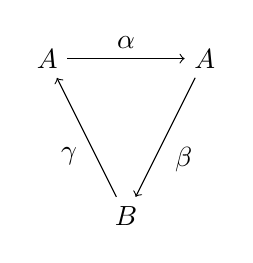
\begin{tikzpicture}
					\node (A) at (-1, 1) {$A$};
					\node (A2) at (1, 1) {$A$};
					\node (B) at (0, -1) {$B$};
					\draw[->] (A) -- node[above]{$\alpha$} (A2);
					\draw[->] (A2) -- node[below right]{$\beta$} (B);
					\draw[->] (B) -- node[below left]{$\gamma$} (A);
				\end{tikzpicture}
				\caption{Exact couple.}
				\label{fig:exact_couple}
			\end{subfigure}
			\begin{subfigure}{0.49\textwidth}
				\centering
				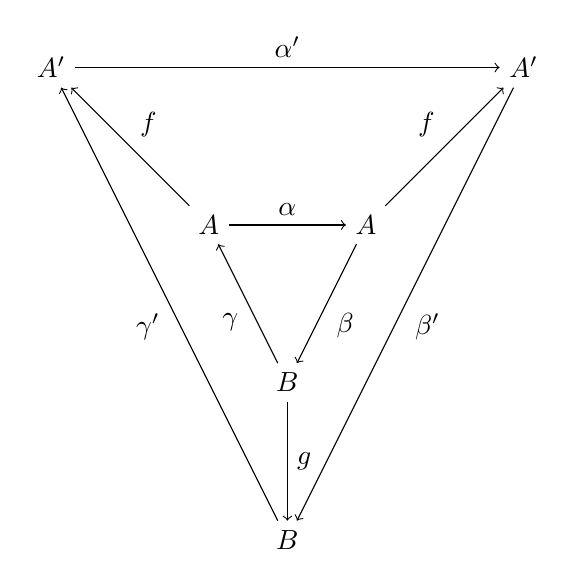
\begin{tikzpicture}
					\node (A') at (-3, 3) {$A'$};
					\node (A2') at (3, 3) {$A'$};
					\node (B) at (0, -1) {$B$};
					\node (A) at (-1, 1) {$A$};
					\node (A2) at (1, 1) {$A$};
					\node (B') at (0, -3) {$B$};
					\draw[->] (A') -- node[above]{$\alpha'$} (A2');
					\draw[->] (A2') -- node[below right]{$\beta'$} (B');
					\draw[->] (B') -- node[below left]{$\gamma'$} (A');
					\draw[->] (A) -- node[above]{$\alpha$} (A2);
					\draw[->] (A2) -- node[below right]{$\beta$} (B);
					\draw[->] (B) -- node[below left]{$\gamma$} (A);
					\draw[->] (A) -- node[above right]{$f$} (A');
					\draw[->] (A2) -- node[above left]{$f$} (A2');
					\draw[->] (B) -- node[right]{$g$} (B');
				\end{tikzpicture}
				\caption{Morphism of exact couples.}
				\label{fig:exact_couple_morphism}
			\end{subfigure}
			\caption{}
			\label{fig:exact_couples_category}
		\end{figure}

		A morphism of exact couples is a pair of morphisms $(f, g):(A, B)\rightarrow (A', B')$ that make the diagram \ref{fig:exact_couple_morphism} commute.
	}

	From any exact couple $(A, B, \alpha, \beta, \gamma)$ one can construct a spectral sequence using the following prescription:
	\begin{align}
		E_0 &= B\\
		d_0 &= \beta\circ\gamma\\
		&\nonumber\\
		E_n &= \frac{\gamma^{-1}(\alpha^n(A))}{\beta(\alpha^{-n}(0))}\\
		d_n &= \beta\circ\alpha^{-n}\circ\gamma
	\end{align}
	It is not so hard to see that $E_{n+1}=H(E_n, d_n)$, so this construction gives a functor from the category of exact couples to the category of spectral sequences. The higher exact couples $(\alpha^nD, E_n, \dots)$ are sometimes called \textbf{derived couples}.

	One can also define the term $E_\infty$ using the following limit procedure: For every $n$ one can look at the elements in $E_n$ that are closed under $d_n$, let's call them $E_{n,n+1}$. Since there exists a canonical surjection $E_{n,n+1}\rightarrow E_{n+1}$ one can then look at all the elements in $E_{n,n+1}$ for which their image in $E_{n+1}$ is closed under $d_{n+1}$ and call these $E_{n,n+2}$. The elements that remain after taking the limit of this operation form the set $E_{n, \infty}$. Now we can also take the (direct) limit of these $E_{n,\infty}$ and this gives us $E_\infty$. This is equivalent to
	\begin{gather}
		E_\infty = \frac{\cap_i Z(E_i)}{\cup_i B(E_i)}.
	\end{gather}
	Hence $E_\infty$ contains the equivalence classes of elements that are cycles for all $d_n$ but boundaries for none. If $E_\infty$ is the associated graded object of some filtered object $G$ then we say that the spectral sequence \textbf{converges} to $G$.

	Now consider a differential object $(C, d)$ together with a filtration\footnote{See definition \ref{set:filtration}.} $\{F_pC\}_{p\in\mathbb{N}}$. The definition of the filtration immediately gives us a short exact sequence for every $p\in\mathbb{N}$:
	\begin{gather}
		0\longrightarrow F_{p-1}C\longrightarrow F_pC\longrightarrow F_pC/F_{p-1}C\longrightarrow 0.
	\end{gather}
	This short sequence then gives rise to a long exact sequence in homology, which can be expressed as an exact triangle, and this triangle in turn leads to an exact couple:
	\begin{gather}
		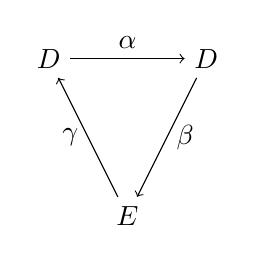
\begin{tikzpicture}
			\node (A) at (-1, 1) {$D$};
			\node (A2) at (1, 1) {$D$};
			\node (B) at (0, -1) {$E$};
			\draw[->] (A) -- node[above]{$\alpha$} (A2);
			\draw[->] (A2) -- node[right]{$\beta$} (B);
			\draw[->] (B) -- node[left]{$\gamma$} (A);
		\end{tikzpicture}
	\end{gather}
	where $D_p = H(F_pC)$ and $E_p=H(F_pC/F_{p-1}C)$. From a more abstract (but at the same time more useful) point of view one can consider the object $E$ as a functor from the category of filtered (differential) objects to the category of graded objects. As such it is constructed from the composition of the homology functor $H$ and the \textit{associated graded object-functor} \[Gr:C\rightarrow \Big\{G_pC := F_pC/F_{p-1}C\Big\}_{p\in\mathbb{N}}.\]

	On the other hand we could of course also construct the composition $Gr\circ H$ which first maps a differential object to its homology object and then builds the graded object associated to the filtration \[F_pH(C):=\im\left(H(F_pC)\rightarrow H(C)\right).\] Now of course some interesting questions arise: ''\textit{How are the functors $H\circ Gr$ and $Gr\circ H$ related?}'', ''\textit{Do they coincide?}'', ... The latter question is easy to answer: ''\textit{No, they do not.}'' However, they can be related and this happens through a spectral sequence that will tell us how the homology of the graded object associated to $C$ can be related to the homology of $C$ itself.

\subsection{Filtered complexes}

	For the remainder of this section we will only consider graded differential objects, i.e. $C_\bullet=\{C_p\}_{p\in\mathbb{Z}}$ for which $dC_p\subseteq C_p$. In this case the exact couple now consist of $D=\{D^{p,q}:=H_q(F_pC_\bullet)\}$ and $E=\{E_{p,q}:=H_q(G_pC_\bullet)\}$ and hence the objects are now bigraded. (The filtration is also required to preserve the differential, i.e. $dF_iC_j\subseteq F_iC_{j-1}$.)

	\sremark{In contrast to most of the literature we did not adopt the \textit{complementary convention}, i.e. the convention where $p+q$ denotes the total degree and hence $E_{p,q}=H_{p+q}(G_pC_\bullet)$.}

	Before we introduce an expression for a general page $E_r$ we will consider the degree zero and one terms to get some intuition. The differential on $E_0$ is given by
	\begin{gather}
		d_0:\frac{F_pC_q}{F_{p-1}C_q}\rightarrow\frac{F_pC_{q-1}}{F_{p-1}C_{q-1}}
	\end{gather}
	and is induced by the differential $d$ on $C_\bullet$. The kernel of this map is clearly given by all elements $x\in F_pC_q$ such that $dx = 0\mod F_{p-1}C_{q-1}$ (with the additional remark that we also have to take the quotient by $F_{p-1}C_q$). As a result we find that the homology $E_1=H(E_0, d_0)$ is given by
	\begin{gather}
		E_1^{p,q}:=\frac{\{x\in F_pC_q: dx\in F_{p-1}C_{q-1}\}}{F_{p-1}C_q+dF_pC_{q+1}}.
	\end{gather}
	The first term in the denominator was already explained above. The second term comes from the $\im(d_0)$ part in the definition of $H(E_0, d_0)$. One might suspect that some data is missing since the relevant map $d_0^{p, q+1}$ goes from $\frac{F_pC_{q+1}}{F_{p-1}C_{q+1}}$ to $\frac{F_pC_q}{F_{p-1}C_{q}}$. However, the image of $F_{p-1}C_{q+1}$ is a subspace of $F_{p-1}C_q$ and this is already included in the first term, so we might as well work with all of $F_pC_{q+1}$.

	For arbitrary $r>0$ we define the page $E_r$ as follows:
	\begin{gather}
	E_r^{p,q}:=\frac{\{x\in F_pC_q: dx\in F_{p-r}C_{q-1}\}}{F_{p-1}C_q+dF_{p+r-1}C_{q+1}}.
	\end{gather}

    ?? COMPLETE ??
\chapter{Logic and Type theory}\label{chapter:type_theory}

    The main reference for this chapter is \cite{hott}. For a formal introduction to $\lambda$-calculus see \cite{lambda_notes}.

    In almost every section of this chapter (at least the ones about type theory) we could have put cross-references to analogous definitions and propositions in other parts of this compendium, in particular the chapter on category theory \ref{chapter:cat}. However, to reduce the number of references we will only mention this and encourage the reader to take a look at \ref{chapter:cat} during or after reading this chapter.

\section{Logic}
\subsection{Languages}

    \newdef{Language}{\index{language}\index{Kleene star}
        An \textbf{alphabet} is a set of symbols. A \textbf{word} in the language is then a string of symbols in the alfabet.

        A more formal way to state the definition of a (formal) language is as follows: Consider an alphabet $A$. From this alphabet one can construct the free monoid $A^*$ (the $\ast$-operator is sometimes called the \textbf{Kleene star}). This monoid represents the set of all words in $A$ and a (formal) language is a subset $L\subseteq A^*$.
    }
    \newdef{Signature}{\index{signature}
        Consider an alphabet $A$ in a language $L$. A signature is a tuple $(F, R, \text{ar})$ that assigns a syntactic meaning to the symbols. $F$ and $R$ are respectively the sets of function symbols and relation symbols $(A=F\cup R)$. The function $\text{ar}:A\rightarrow\mathbb{N}$ assigns to every symbol its arity \textbf{arity} $n$. Nullary function symbols are also called \textbf{constants}.
    }

    To give meaning to a language we have to add some extra structure:
    \newdef{$L$-structure}{\index{universe}
        Consider a (formal) language $L$. An $L$-structure consists of the following data:
        \begin{enumerate}
            \item A nonempty set $U$ called the \textbf{universe}.
            \item For each function symbol $f$ a function $\text{ap}_f:U^{\text{ar}(f)}\rightarrow U$. In particular, for each constant $c$ an element $u_c\in U$.
            \item For each relation symbol $\in$ a set $R_\in\subseteq U^{\text{ar}(\in)}$.
        \end{enumerate}
    }

    \newdef{$L$-term}{\index{term}\index{variable}
        A word in $L$ possibly containing new symbols, called \textbf{variables}, defined recursively as follows:
        \begin{enumerate}
            \item Every variable and every constant is a term.
            \item If $f$ is an $n$-ary function symbol and $x_1,\ldots,x_n$ are terms then so is $f(x_1,\ldots,x_n)$.
        \end{enumerate}
    }
    \newdef{$L$-formula}{\index{formula}
        Consider a (formal) language $L$. An $L$-formula is a sentence in $L$ consisting of terms in $L$ together with parentheses and logical symbols (also called \textbf{logical connectives}):
        \begin{itemize}
            \item \textbf{Equality}: $=$,
            \item \textbf{Negation}: $\lnot$,
            \item \textbf{Conjunction}: $\land$, and
            \item \textbf{Existential quantifier}: $\exists$.
        \end{itemize}
        A variable is said to be \textbf{free} if it does not first appear next to a quantifier, otherwise it is said to be \textbf{bound}.
    }

\subsection{Propositional logic}

    \newdef{Proposition}{\index{proposition}
        A statement that is either true or false (not both).
    }
    \newdef{Paradox}{\index{paradox}
        A statement that cannot (consistently) be assigned a truth value.
    }

    \newdef{Contradiction}{\index{contradiction}
        A statement that is always false.
    }
    \newdef{Tautology}{\index{tautology}
        A statement that is always true.
    }

    \begin{notation}[Truth values]
        The truth values \textit{true} and \textit{false} are denoted by $\top$ and $\bot$ respectively.
    \end{notation}

    \newdef{Logical connectives}{
        As basic logical operators we introduce the following symbols:
        \begin{itemize}
            \item Logical and (\textbf{conjunction}): $P\land Q$,
            \item Logical or (\textbf{disjunction}): $P\lor Q$, and
            \item Logical not (\textbf{negation}): $\lnot P$.
        \end{itemize}
        This last symbol is in fact an abbreviation for the implication $P\rightarrow\bot$.
    }

    The basic inference rule is given by \textbf{modus ponens}:
    \begin{gather}
        \text{If } P \text{ and } P\rightarrow Q \text{ then } Q.
    \end{gather}
    The general deductive system for propositional logic is obtained by combining this rule with the following axioms:
    \begin{enumerate}
        \item If $P$ then $Q\rightarrow P$.
        \item If $P\rightarrow Q \rightarrow R$ then $P\rightarrow Q$ implies $P\rightarrow R$.
        \item If $P\land Q$ then both $P$ and $Q$.
        \item If $P$ then $P\lor Q$.
        \item If $Q$ then $P\lor Q$.
        \item If $P$ then $Q$ implies $P\land Q$.
        \item If $P\rightarrow Q$ then $R\rightarrow Q$ implies $P\lor R\implies Q$.
        \item If $\bot$ then $P$. This principle is often called \textbf{ex false quodlibet}.
    \end{enumerate}

    \begin{remark}[Intuitionistic logic]
        The above axioms (together with the inference rule) define a specific type of propositional logic, called intuitionistic or \textbf{constructive} (propositional) logic. The main difference with classic logic is that we did not add the \textit{law of the excluded middle} or, equivalently, the \textit{double negation elimination} principle. The reason why this makes the logic \textit{constructive} is that to prove a statement it is not enough anymore to exclude the possibility of the statement being false. One has to explicitly construct evidence for the truth of the statement.

        As was remarked in the chapter on topoi, intuitionistic logic can be defined internal to any elementary topos. All we need is a Heyting algebra \ref{set:heyting}. ?? DO THIS ??
    \end{remark}

\subsection{Predicate logic}

    ?? COMPLETE ??

\section{Introduction to type theory}

    In ordinary set theory the main objects are sets and their elements (and if we want we can construct extra concepts such as functions). The frame work in which we work to state and prove propositions is (in general) given by first-order logic. See section \ref{set:section:axiomatization} for more on this.

    In type theory however, we put all these notions on the same footing. That is, we consider all concepts such as functions, propositions, sets, ... as specific instances of the general notion of \textit{type}. A specific function, proof or element can then be seen as an \textit{inhabitant} of the type under consideration.

    \begin{method}[Type definition]
        The general method for the definition of a new type consists of 4 rules:
        \begin{enumerate}
            \item \textbf{Formation rule}: This rule tells us when the new type can be introduced (possibly using simpler types).
            \item \textbf{Introduction rule}: This rule gives a \textbf{constructor} of the new type (possibly based on type judgements of simpler types).
            \item \textbf{Elimination rule}: This rule tells us what we can do with the new type.
            \item \textbf{Computation rule}: This rule tells us how the elimination and introduction rules interact.
        \end{enumerate}
    \end{method}
    \newdef{Type judgement}{\index{type!judgement}\index{term}
        A judgement of the form $a:A$, saying that $a$ has the type $A$, is called a type judgement. Objects having a certain type are in general called \textbf{terms} (of that type).
    }

    As in \cite{hott} we will work with a universe hierarchy \`a la Russell, i.e. we work with a sequence of universes $(\mathcal{U}_i)_{i\in\mathbb{N}}$ such that the terms of every universe are types and every universe is cumulative $A:\mathcal{U}_i\implies A:\mathcal{U}_{i+1}$. In general we will omit subscripts, but one should take into account that every well-typed judgement should admit a formulation in which subscripts can be assigned in a consistent way.

    In contrast to ordinary set theory we will introduce two kinds of equality. First we have the \textbf{judgemental equality} or \textbf{definition equality}. This says, as the name implies, that two judgements are equal by definition and as such its validity lives in the metatheory (it is not a proposition and hence cannot be proven). For example if $f(x)$ is defined as $x^2$ then $f(5)$ is by definition equal to $5^2$. Equalities of this sort will be denoted by the $\equiv$ symbol (and in definitions we will use $:\equiv$ instead of $:=$). The second equality is the \textbf{propositional equality}. This states that two judgements are provably equal. Again we consider the function $f(x):\equiv x^2$. In this case the proposition $f(5)=25$ can be proven, but it is not true by definition (it would depend on the definition of the natural numbers). This sort of equality will be denoted by an ordinary equals sign $=$.\index{equality}

\section{Basic constructions}
\subsection{Functions}

    Functions can be introduced in two ways. Either through a direct definition, such as in the case of our default example $f(x):\equiv x^2$, or through $\lambda$-abstraction. Although the former one is clearly more useful during explicit calculations, we will often utilize the latter when working with abstract proofs. (For an introduction to $\lambda$-calculus see the next section.)

    \newdef{Function type}{\index{function}
        A general function type is introduced as follows:
        \begin{itemize}
            \item \textbf{Formation rule}: Given two types $\type{A,B}$ one can form the function type $\type{A\rightarrow B}$.
            \item \textbf{Introduction rule}: One can either define a function by an explicit definition $f(x):\equiv\Phi$, where $\Phi$ is an expression possibly involving $x$, or by $\lambda$-abstraction $f:\equiv\lambda x.\Phi$.
            \item \textbf{Elimination rule}: If $a:A$ and $\lambda x.\Phi:A\rightarrow B$ then $\lambda x.\Phi(a):B$.
            \item \textbf{Computation rule}\footnote{In $\lambda$-calculus this is often called $\beta$-reduction. (See the next section.)}: $\lambda x.\Phi(a):\equiv\Phi(a)$, i.e. function application is equivalent to the subsitution\footnote{In technical terms we require the substitution to be \textit{capture-avoiding}.} of $a$ for the variable $x$ in the expression $\Phi$.
        \end{itemize}
        We will also include the uniqueness principle for function types in the definition, i.e. $\lambda x.f(x)\equiv f$. This says that every function is uniquely defined by its image.
    }

    An important generalization is obtained when we allow the type of the output of a function to depend on the type of the input:
    \newdef{Dependent function types}{
        Given a type $\type{A}$ and a type family $\typef{B}{A}$ one can form the dependent function type \[\type{\prod_{a:A}B(a)}.\] In the case that $B$ is a constant family this type reduces to the ordinary function type $A\rightarrow B$. All other defining rules remain (formally) the same as in the nondependent setting.
    }
    \begin{example}[Polymorphic functions]\index{polymorphicity}
        An interesting example is obtained when we take the type $A$ in the above definition to be a universe $\mathcal{U}$ (which is a valid choice since universes are types themselves) together with $B(A):\equiv A$. In this case one obtains a function that takes a type as input and then acts on this type (or any other type constructed from it), e.g. the \textbf{polymorphic identity function}
        \begin{gather}
            \text{id}:\prod_{\type{A}}A\rightarrow A
        \end{gather}
        defined by
        \begin{gather}
            \text{id}:\equiv\lambda(\type{A}).\lambda(a:A).a.
        \end{gather}
    \end{example}

    \remark{The $\Pi$-symbol scopes over the rest of the expression, unless delimited, e.g. \[\prod_{a:A}B(a)\rightarrow C(a)\equiv\prod_{a:A}\Big(B(a)\rightarrow C(a)\Big).\]}

\subsection{\texorpdfstring{$\lambda$-calculus}{Lambda-calculus}}

    ?? COMPLETE (e.g. Curry-Howard or even Curry-Howard-Lambek, typed vs. untyped calculus, ...)??

\subsection{Identity types}

    One of the most important, but at the same time most subtle, concepts in type theory (especially when going to extensions such as homotopy type theory) is that of an identity type. Since in predicate (and even propositional) logic the equality of two terms is a proposition, we expect that to every two terms $a,b:A$ (for some given type) there corresponds an associated equality type $\type{a=_Ab}$. Note that the type of the terms is assumed to be the same since it does not make any sense to compare terms of different types.

    \newdef{Equality type\footnotemark}{\index{equality}
        \footnotetext{Sometimes called an \textbf{identity type}.}
        The type corresponding to a propositional equality is defined by the following rules:
        \begin{itemize}
            \item \textbf{Formation rule}: Given terms $a,b:A$ one can form the equlity type $\type{a=_Ab}$. When the type $A$ is clear from the context then this is also often written as $\type{a=b}$.
            \item \textbf{Introduction rule}: For every term $a:A$ there is a canonical identity element
            \begin{gather}
                \text{refl}_a:a=a.
            \end{gather}
            The notation points to the fact that this term can be seen as a proof of the reflexivity of equality.
            \item \textbf{Elimination and computation rules}: Here we present the so-called \textbf{path induction principle} for equality types (for the equivalent \textit{based path induction principle} we refer to \cite{hott}). If we are given a type family \[C:\prod_{a,b:A}a=b\rightarrow\mathcal{U}\] and a term \[I:\prod_{a:A}C(a, a, \text{refl}_a)\] then there exists a function
            \begin{gather}
                f:\prod_{a,b:A}\prod_{p:a=b}C(a,b,p)
            \end{gather}
            such that
            \begin{gather}
                f(a,a,\text{refl}_a):\equiv I(a)
            \end{gather}
            for all $a:A$.
        \end{itemize}
        Informally this principle says that all terms of the form $(a,b,p)$, with $p:a=b$, are inductively generated by the ''constant'' terms $(a,a,\text{refl}_a)$. (See the section on homotopy type theory for a more geometric perspective).
    }

    Using the notion of identity types one can say when a given type resembles a proposition:
    \newdef{Mere proposition}{\index{proposition}
        A type $\type{A}$ is sadi to be a (mere) proposition if the type
        \begin{gather}
            \text{isProp}(A):\equiv\prod_{a,b:A}a=b
        \end{gather}
        is inhabited.
    }

\subsection{Products}

    As in classic set theory a basic notion is that of products. This construction is ubiquitous throughout all corners of mathematics (and computer science). However, as opposed to set theory \`a la ZFC, products are not explicitly constructed as the set of all pairs of elements of its constituents. On the contrary, in type theory one can prove that all elements necessarily have to be pairs.

    \newdef{Product}{\index{product}\index{recursion}\index{induction}\index{unit!type}\index{projection}\index{pairing}
        We first define the binary product of types:
        \begin{itemize}
            \item \textbf{Formation rule}: Given any two types $\type{A, B}$ one can form the product type $\type{A\times B}$.
            \item \textbf{Introduction rule}: Given terms $a:A, b:B$ one can construct the term $(a,b):A\times B$. This is called the \textbf{pairing} of the terms $a:A,b:B$.
            \item \textbf{Elimination and computation rules}: First we will introduce the \textbf{projections}, analogous to the projection functions associated to the set-theoretic Cartesian product: If $x:A\times B$ then $\pi_1(x):A$ and $\pi_2(x):B$. On the constructor these should act as we expect:
            \begin{gather}
                \pi_1(a,b):\equiv a\qquad\qquad\qquad\pi_2(a,b):\equiv b
            \end{gather}

            More generally we would like to be able to define functions out of a product $A\times B$. We require these functions to be defined through currying, i.e. given a function $A\rightarrow B\rightarrow C$ we can define a function $A\times B\rightarrow C$. Instead of giving an explicit definition every time we want to construct a new function, we adapt a universal point of view (one function that turns terms $f:A\rightarrow B\rightarrow C$ into terms $g:A\times B\rightarrow C$). To this end we define the \textbf{recursor}:
            \begin{gather}
                \text{rec}_{A\times B}: \prod_{\type{C}}(A\rightarrow B\rightarrow C)\rightarrow A\times B\rightarrow C
            \end{gather}
            with the constraint
            \begin{gather}
                \text{rec}_{A\times B}(C, f, (a,b)):\equiv f(a)(b).
            \end{gather}
            Using the recursor we can define the projections $\pi_1,\pi_2$ by taking $C=A, f=\lambda a.\lambda b.a$ and $C=B, f=\lambda a.\lambda b.b$ respectively.
        \end{itemize}

        As usual we can also define a nullary product. In this case it is called the \textbf{unit type} $\mathbf{1}$:
        \begin{itemize}
            \item \textbf{Formation rule}: $\type{\mathbf{1}}$.
            \item \textbf{Introduction rule}: There is a unique nullary constructor $\ast:\mathbf{1}$.
            \item \textbf{Elimination and computation rules}: Since the constructor is a nullary operation we do not expect to have projection maps and likewise we also do not expect function definition to be based on binary currying. Instead we define the recursor as follows:
            \begin{gather}
                \text{rec}_{\mathbf{1}}:\prod_{\type{C}}C\rightarrow\mathbf{1}\rightarrow C.
            \end{gather}
            On the constructor $\ast:\mathbf{1}$ we require it to act trivially:
            \begin{gather}
                \text{rec}_{\mathbf{1}}(C, c_0, \ast):\equiv c_0.
            \end{gather}
        \end{itemize}
        We can easily generalize the above recursion functions to \textbf{induction} functions, to allow for the definition of dependent functions (these functions are then said to be defined by an \textbf{induction principle}). In fact, we only have to change the type judgement of $\text{rec}_{A\times B}$. This is accomplished by replacing $\type{C}$ by a type family $\typef{C}{A\times B}$ and by replacing nondependent function types by dependent function types (the form of the computation rules remain formally the same):
        \begin{align}
            \text{ind}_{A\times B}&:\prod_{\typef{C}{A\times B}}\left(\prod_{a:A}\prod_{b:B}C(a,b)\rightarrow\prod_{x:A\times B}C(x)\right)\\
            &\nonumber\\
            \text{ind}_{\mathbf{1}}&:\prod_{\typef{C}{\mathbf{1}}}C(\ast)\rightarrow\prod_{x:\mathbf{1}}C(x).
        \end{align}
    }

    \begin{property}[Uniqueness principle]
        Using the induction principle introduced above, one can prove that every term $x:A\times B$ is necessarily of the form $(a,b)$ for some $a:A, b:B$. Furthermore, one can also prove that $\ast:\mathbf{1}$ is the unique term in $\mathbf{1}$.
    \end{property}

    Like we did for functions, we can also generalize products such that the type of the second factor depends on the type of the first one. In classical set theory this would correspond to an indexed disjoint union:
    \newdef{Dependent pair type}{\index{pair}\index{$\Sigma$-type}
        As with function types we will not work out the definition as explicit as the one for nondependent types. Suffice it to say that given a type $\type{A}$ and a type family $\typef{B}{A}$ one can form the dependent pair type \[\type{\sum_{a:A}B(a)}.\] In the case that $B$ is a constant family, the type reduces to the ordinary product type $A\times B$. The recursor and induction functions are defined as in the product case, except for the obvious replacements, such as $A\times B\longrightarrow\sum_{a:A}B(a)$, needed to make everything consistent.
    }
    \remark{Dependent pair types are often called \textbf{$\Sigma$-types} (due to the notation).}
    \remark{Like the $\Pi$-symbol, the $\Sigma$-symbol scopes over the rest of the expression unless delimited.}

    Analogous to the product one can also define the coproduct:
    \newdef{Coproduct}{\index{coproduct}\index{injection}
        Here we give a formal standalone definition, the relation with the ordinary product will be mentioned afterwards.
        \begin{itemize}
            \item \textbf{Formation rule}: Given two types $\type{A,B}$ one can form the coproduct type $\type{A+B}$.
            \item \textbf{Introduction rule}: Since in ordinary mathematics (and in particular category theory) the coproduct is dual to the product we expect the projections to be replaced by \textbf{injections}/\textbf{inclusions}. In fact we will take them to be the constructors of coproduct types, i.e. given terms $a:A, b:B$ we can construct the terms $\iota_1(a):A+B$ and $\iota_2(b):A+B$.
            \item \textbf{Elimination rules}: Similar to the use of currying for the definition of functions out of a product, we will decompose functions out of a coproduct. To this intent we define the recursion and induction functions as follows:
            \begin{align}
                \text{rec}_{A+B}&:\prod_{\type{C}}(A\rightarrow C)\rightarrow(B\rightarrow C)\rightarrow A+B\rightarrow C\\
                \text{ind}_{A+B}&:\prod_{\typef{C}{A+B}}\left(\prod_{a:A}C(\iota_1(a))\right)\rightarrow\left(\prod_{b:B}C(\iota_2(b))\right)\rightarrow\prod_{x:A+B}C(x).
            \end{align}
            \item \textbf{Computation rules}: The recursion function acts on the constructors as follows (the induction function formally has the same action):
            \begin{align}
                \text{rec}_{A+B}(C, f_1, f_2, \iota_1(a))&:\equiv f_1(a)\\
                \text{rec}_{A+B}(C, f_1, f_2, \iota_2(b))&:\equiv f_2(b).
            \end{align}
        \end{itemize}

        As was the case for products one can also define a nullary version of the coproduct (the \textbf{empty type} $\mathbf{0}$):
        \begin{itemize}
            \item \textbf{Formation rule}: $\type{\mathbf{0}}$.
            \item \textbf{Introduction rule}: There is no constructor for $\mathbf{0}$.
            \item \textbf{Elimination and computation rules}: Since there is no constructor for $\mathbf{0}$, we can always trivially ''construct'' a function out of $\mathbf{0}$:
            \begin{align}
                \text{rec}_{\mathbf{0}}&:\prod_{\type{C}}\mathbf{0}\rightarrow C\\
                \text{rec}_{\mathbf{0}}&:\prod_{\typef{C}{\mathbf{0}}}\prod_{x:\mathbf{0}}C(x).
            \end{align}
            This trivial function corresponds to the logical principle \textit{ex falso quodlibet} as introduced in the section on logic above.
        \end{itemize}
    }

    Since coproducts in set theory occur as binary disjoint unions, one can expect that there is a way to express coproducts in terms of dependent pair types:
    \begin{construct}[Coproducts as $\Sigma$-types]
        Let us first introduce the type $\type{\mathbf{2}}$ (in set theory this would be the 2-element set). The introduction rule constructs two terms $0,1:\mathbf{2}$. The elimination and computation rules tell us that we can use this type for binary indexing:
        \begin{gather}
            \text{rec}_{\mathbf{2}}:\prod_{\type{C}}C\rightarrow C\rightarrow\mathbf{2}\rightarrow C
        \end{gather}
        with
        \begin{align}
            \text{rec}_{\mathbf{2}}(C, c_0, c_1, 0)&:\equiv c_0\\
            \text{rec}_{\mathbf{2}}(C, c_0, c_1, 1)&:\equiv c_1.
        \end{align}
        Using this type one can prove that $A+B$ is judgementally equal to $\sum_{x:\mathbf{2}}\text{rec}_{\mathbf{2}}(\mathcal{U}, A, B, x)$. The injections are then given by pairing, i.e. $\iota_1(a)\equiv(0, a)$ and $\iota_2(b)\equiv(1, b)$.\footnote{In a similar way one can obtain binary products as dependent function types over $\mathbf{2}$. In this case pairing is obtained through the induction principle for $\mathbf{2}$.}
    \end{construct}

\subsection{Natural numbers}

    ?? COMPLETE ??

\subsection{Propositions as types}

    To conclude this section we give an overview of all the concepts we introduced before from a propositions-as-types perspective (in intuitionistic logic this is often called the \textit{Brouwer-Heyting-Kolmogorov} interpretation and more specific it should be seen as an incarnation of the Curry-Howard correspondence).

    \begin{itemize}
        \item Types and their terms correspond to propositions and their proofs respectively. In a proof-relevant context the fact that a type can have multiple terms makes it clear that, although distinct proofs eventually have the same result, the difference in their content can be important as well.
        \item Function types correspond to implications. A proof of the proposition $A\rightarrow B$ boils down to showing that every proof of $A$ gives a proof of $B$.
        \item $\Pi$-types correspond to universal quantification, i.e. $\prod_{a:A}B(a)$ can be read as $\forall a\in A: B(a)$. Giving a proof of $\prod_{a:A}B(a)$ is the same as giving for every $a:A$ a proof of $B(a)$. This is indeed compatible with the fact that elements of $\Pi$-types are dependent functions, i.e. every element $a:A$ gives rise to a (possibly) distinct type/proposition.
        \item $\Sigma$-types correspond to existential quantification, i.e. $\sum_{a:A}B(a)$ can be read as $\exists a\in A:B(a)$. Giving a proof of $\sum_{a:A}B(a)$ is the same as giving a proof for some $(a, B(a))$. This is compatible with the fact that $\Sigma$-types can be identified with disjoint unions and hence every element can be associated with a specific constituent type.
        \item The logical connectives, conjunction and disjunction, can be obtained in a similar way as the product and coproduct types.
        \item The truth values, \textit{true} and \textit{false}, correspond to the unit and empty types respectively. Furthermore, if we define the negation of $A$ as the type $\lnot A:\equiv A\rightarrow\mathbf{0}$, then this indeed corresponds to the logical negation by the statements above.
    \end{itemize}

\section{Homotopy type theory}\nomenclature[A_HOTT]{HoTT}{Homotopy Type Theory}
\subsection{Introduction}

    In this section we will reformulate (or extend) the previous section using the language of homotopy theory (and more generally algebraic topology), section \ref{section:homotopy}, and (weak) $\infty$-groupoids, section \ref{section:groupoids}. The resulting theory is called homotopy type theory or \textbf{HoTT}. From here one we will use this abbreviation.

    The general idea will be that we will associate types with topological spaces and terms with points in those spaces. The main novelty is given by the identification of (propositional) equalities with paths between points. Since we work in a proof-relevant context, we do not consider two equalities $p,q:a=_Ab$ to be necessarily equal themselves and hence we can consider equalities between equalities (and so on). In the topological picture this gives us homotopies between paths. If we go all the way and work out all coherence laws, we obtain the structure of a (weak) $\infty$-groupoid.\footnote{This characterization is strongly related to the homotopy hypothesis (or theorem if we use the right model for $\infty$-categories).}

    It is also this interpretation that explains the name ''path induction'' for the induction principle of equality types. Namely what this induction principle says is that the free path space $\Omega A$ is inductively generated by constant loops (ranging over all possible points). This principle however sounds quite crazy, how can one built a path between two distinct points from (constant) loops at a point. Here it is important to remind that everything only has to be equal up to homotopy and any path is indeed equivalent to a constant loop (up to homotopy) if we retract one of the endpoints along the path. It is thus important that we do not require the homotopies to act rel endpoints (as is often done in classic homotopy theory).

    \newdef{Pointed type}{\index{pointed!type}
        A pointed type is a type $\type{A}$ together with a distint term $a:A$, called its basepoint. Pointed types are often denoted by a pair $(A, a)$. It should be clear that the type of pointed types is equal to $\sum_{\type{A}}A$ (it is sometimes denoted by $\mathcal{U}_\bullet$).
    }
    \newdef{Loop space}{\index{loop!space}
        The loop space $\Omega(A, a)$ of a pointed type $(A, a)$ is the pointed type $(a=_Aa, \text{refl}_a)$. Terms of this type are called \textbf{loops}.
    }

    Now the important aspect of HoTT is that the $\infty$-groupoid structure of a type can be derived solely from the (path) induction principle of the equality types. We give some examples:
    \begin{property}[Inversion]
        For every type $\type{A}$ and terms $a,b:A$ there exists a function
        \begin{gather}
            p\mapsto p^{-1}:(a=b)\rightarrow(b=a)
        \end{gather}
        such that $\text{refl}_a^{-1}:\equiv\text{refl}_a$ for all $a:A$.
    \end{property}
    \begin{property}[Concatenation]
        For every type $\type{A}$ and terms $a,b,c,d:A$ there exists a function
        \begin{gather}
            p\mapsto q\mapsto p\sqdot q:(a=b)\rightarrow(b=c)\rightarrow(c=d)
        \end{gather}
        such that $\text{refl}_a\sqdot\text{refl}_a:\equiv\text{refl}_a$ for all $a:A$. (Note that the composition does not follow the usual convention of right-to-left. This is why we used the symbol $\sqdot$ and not $\circ$.)
    \end{property}
    \begin{property}
        The above operations satisfy the group relations (up to higher equalities):
        \begin{itemize}
            \item $p\sqdot\text{refl}_b=p$ and $\text{refl}_a\sqdot p=p$ for all $p:a=b$.
            \item $p\sqdot p^{-1}=\text{refl}_a$ and $p^{-1}\sqdot p=\text{refl}_b$ for all $p:a=b$.
            \item $(p^{-1})^{-1}=p$ for all $p:a=b$.
            \item $p\sqdot(q\sqdot r) = (p\sqdot q)\sqdot r$ for all $p:a=b, q:b=c, r:c=d$.
        \end{itemize}
    \end{property}

\subsection{Transport}

    The relation with homotopy theory and category theory becomes even stronger if we look at function types:
    \begin{property}
        Given a function $f:A\rightarrow B$ there exists a function (sometimes called an \textbf{application function}\footnote{Because of this some authors denote this function by $\text{ap}_f$.})
        \begin{gather}
            f:(a=_Ab)\rightarrow(f(a)=_Bf(b))
        \end{gather}
        such that $f(\text{refl}_a):\equiv\text{refl}_{f(a)}$ for all $a, b:A$. Furthermore, this function behaves functorially in that it preserves concatenation, inverses and identities (again this should be interpreted in the full weak $\infty$-sense). This also explains the reason for our abuse of notation: In category theory functors acting on objects and on morphisms are generally given the same notation. From the topological perspective this can be interpreted as if all functions are ''continuous''.
    \end{property}
    For dependent functions one can obtain a similar result. However, for this generalization, we first need some kind of ''parallel transport'' since for two terms, such that $a=b$, it does not necessarily hold that $f(a)$ and $f(b)$ have the same type.
    \begin{property}[Transport]\index{fibration}\index{transport}\index{lift}\index{section}
        Given a type family $\typef{P}{A}$ and an equality $p:a=_Ab$  there exists a \textbf{transport function}
        \begin{gather}
            p_*:P(a)\rightarrow P(b)
        \end{gather}
        such that $(\text{refl}_a)_*:\equiv\text{id}(a)$ for all $a:A$. We have used the pushforward-notation since $p_*$ can be (informally) interpreted as the pushforward of $p$ along $P$.

        This transport function lets us, from a topological perspective, regard type families as fibrations, i.e. continuous functions $\pi:E\rightarrow B$ having the path lifting property. For every type family $\typef{P}{A}$, term $\alpha:P(a)$ and equality $p:a=b$ there exists a \textbf{lift}
        \begin{gather}
            \text{lift}(p, \alpha):(a, \alpha) = (b, p_*(\alpha)).
        \end{gather}
        such that
        \begin{gather}
            \pi_1(\text{lift}(p, u))=p.
        \end{gather}
        The equality $\text{lift}(p, u)$ acts between terms of the $\Sigma$-type $\sum_{a:A}P(a)$, which can be interpreted as the total space of a \textbf{fibration} $\pi_1:\sum_{a:A}P(a)\rightarrow A$. To take this terminology even further, one can could call functions $\sigma:\prod_{a:A}P(a)$ \textbf{sections} (of $\pi_1$).
    \end{property}
    Now, as we mentioned before, for dependent functions we cannot just compare $f(a)$ and $f(b)$ if $a\not\equiv b$. However, the function $\text{lift}(p, \cdot)$ gives us a canonical path from one fibre to the other and we expect that every path between these fibres should factor through this canonical one essentially uniquely. Hence we can define a path between $\alpha$ and $\beta$ in the total space $\sum_{a:A}P(a)$, lying over $p:a=b$, to be a path $p_*(\alpha)=\beta$ (up to equivalence):
    \begin{property}
        Given a dependent function $f:\prod_{a:A}P(a)$ there exists a function (again with some abuse of notation)
        \begin{gather}
            f:\prod_{p:a=b}p_*(f(a))=_{P(b)}f(b).
        \end{gather}
        Analogous to the nondependent case, some authors use the notation $\text{apd}_f$.
    \end{property}

    Since ordinary functions are a specific instance of $\Pi$-types, we might expect that the application functions $\text{ap}_f$ and $\text{apd}_f$ are related in this case. This intuition is not unreasonable:
    \begin{property}
        Consider two type $\type{A, B}$ and a function $f:A\rightarrow B$. For every equality $p:a=_Ab$ and term $\alpha:P(b)$ there exists an equality $\widetilde{p}:p_*(\alpha)=_{P(b)}\alpha$. Using this equality one can then relate the application functions as follows:
        \begin{gather}
        \text{apd}_f(p) = \widetilde{p}(f(a))\sqdot\text{ap}_f(p).
        \end{gather}
    \end{property}

\subsection{Equivalences}

    In this paragraph we want to delve a bit deeper into the notion of equivalences and isomorphisms since, as we now from the chapter on category theory, the distinction between the various notions of similarity (or equality) are important but can be very subtle.

    Let by the intuition from topology we first introduce a \textbf{homotopy} between functions:
    \newdef{Homotopy}{\index{homotopy}
        Consider two sections $f,g:\prod_{a:A}P(a)$. A homotopy between $f$ and $g$ is a term of the type
        \begin{gather}
            f\sim g:\equiv\prod_{a:A}f(a)=g(a).
        \end{gather}
        It can be shown that homotopies induce equivalence relations on function types.
    }
    We have already seen that functions can be regarded as functors between $\infty$-groupoids. Since homotopies act between functions we might expect that we can regard these as (weak) natural transformations between the ($\infty$-)functors:
    \begin{property}
        Consider two sections $f,g:\prod_{a:A}P(a)$ and an equality $p:a=b$. If $H$ is a homotopy between $f$ and $g$ then:
        \begin{gather}
            H(a)\sqdot g(p) = f(p)\sqdot H(b).
        \end{gather}
    \end{property}

    Using the notion of homotopy one can introduce a first kind of ''equivalence'':
    \newdef{Quasi-inverse}{\index{inverse!quasi}
        Given a function $f:A\rightarrow B$, we call the triple $(g, \alpha, \beta)$, where $g:B\rightarrow A$ and $\alpha, \beta$ are 2 homotopies, if
        \begin{gather}
            \alpha:f\circ g\sim\text{id}_B\qquad\qquad\qquad\beta:g\circ f\sim\text{id}_B.
        \end{gather}
        From a homotopy theoretical perspective we would call the pair $(f, g)$ a homotopy equivalence. The corresponding type is given by
        \begin{gather}
            \text{qInv}(f):\equiv\sum_{g:B\rightarrow A}(f\circ g\sim\text{id}_B)\times(g\circ f\sim\text{id}_A).
        \end{gather}
    }
    Now, although this type may seem to give the right notion of equivalence, it is better to generalize it since it is in general not very well-behaved. (This is similar to the fact that adjoint equivalences between categories are better behaved than ordinary equivalences.)

    In general we want an equivalence to satisfy three requirements:
    \begin{enumerate}
        \item For every function $f:A\rightarrow B$ there exists a function $\text{qInv}(f)\rightarrow\text{isEquiv}(f)$.
        \item For every function $f:A\rightarrow B$ there also exists a function $\text{isEquiv}(f)\rightarrow\text{qInv}(f)$.
        \item For every two terms $eq_1, eq_2:\text{isEquiv}(f)$ there exists an equality $eq_1=eq_2$.
    \end{enumerate}
    So, inducing an equivalence is logically equivalent to admitting a quasi-inverse and as such finding a quasi-inverse is sufficient to show that a function induces an equivalence.

\subsection{Equality types: revisited}

    In the previous section on (intensional) type theory we introduced equality types in a general and uniform way. The defining rules did not assume any specific structure of the underlying types. Although this made the technique of path induction widely applicable, it has the downside that we cannot leverage the internal structure of specific types to get more useful characterizations.

    Let us first consider binary products (and by extension $\Sigma$-types). Can we express the equality of two elements $x,y:A\times B$ in terms of their projections? The answer is yes: there exists an equivalence
    \begin{gather}
        (x=_{A\times B}y)\simeq(\pi_1(x)=_A\pi_1(y))\times(\pi_2(a)=_B\pi_2(y)).
    \end{gather}
    However, we should bear in mind that this is merely an equivalence. A term (resp. proof) of one side gives a term (resp. proof) of the other side, but it is not a judgemental equality (it is not even a propositional one). One could see this as a problem or defect of the theory and to resolve this kind of (apparent) issue we will introduce the univalence axiom at the end of this section. Still one can leverage this equivalence to give a practical alternative\footnote{Note that this is not a judgementally equal alternative. It is merely a convenient interpretation.} for the defining rules of the equality type in the case of product types:
    \begin{remark}
        The function $(\pi_1(a)=\pi_1(b))\times(\pi_2(a)=\pi_2(b))\rightarrow(a=b)$ associated to the above equivalence can be interpreted as an introduction rule of the equality type for binary products. At the same time one can take the application functions induced by the projections on $A\times B$ as elimination rules for the equality type. The homotopies associated to the equivalence in their turn induce the propositional computation rules and uniqueness principle.
    \end{remark}

    One can also express the transport of properties along an equality $p:x=_{A\times B}y$ in terms of transport in the individual spaces:
    \begin{property}
        Consider two types $\type{A, B}$ together with type families $\typef{P}{A}$ and $\typef{Q}{B}$. For every term $\alpha$ of the product family $(P\times Q)(x):\equiv P(\pi_1(x))\times Q(\pi_2(x))$ the following equality is inhabited:
        \begin{gather}
            p_*(\alpha) = \big(p_*(\pi_1(\alpha)), p_*(\pi_2(\alpha))\big).
        \end{gather}
        Here, we have indulged in the (ab)use of the notation $p_*$. One should note that all three occurrences denote a different operation (or more precise: the same operation, but on different types).
    \end{property}

    One would intuitively expect that given two functions $f,g:A\rightarrow B$ that take the same value at all points, i.e. $f(a)=g(a)$ for all $a:A$, these two functions are equal, i.e. $f=_{A\rightarrow B}g$. However, this cannot be proven within the frame work of intensional type theory. This issue should also not come as a shock, since two functions that are defined differently might still take the same value at all points. To resolve this apparent gap in the theory we introduce the following axiom:
    \begin{axiom}[Function extensionality]
        Given two functions $f,g:\prod_{a:A}P(a)$ there exists an equivalence $(f=g)\rightarrow\prod_{a:A}f(a)=g(a)$ which sends $\text{refl}_f$ to $f(\text{refl}_x)$.
    \end{axiom}
    \begin{axiom}[Univalence axiom]\index{univalence}
        Given two types $\type{A,B}$ there exists an equivalence $(A=_{\mathcal{U}}B)\rightarrow(A\simeq B)$ which takes $\text{refl}_A$ to $\text{id}_A$. A universe in which the univalence axiom holds is said to be univalent.
    \end{axiom}

    ?? COMPLETE ??

\section{Modal type theory}\label{section:modal_type_theory}

    ?? COMPLETE ??

\section{Computability theory}\label{section:turing}
\subsection{Functions}

    \newdef{Recursively enumerable set}{\index{set!enumerable}
        A set $S$ of natural numbers is set to be recursively (or \textbf{computably}) enumerable if there exists a partial recursive function $f$ such that $\dom(f)=S$.
    }

    \newdef{Uniformly recursively enumerable}{
        A sequence $\seq{S}$ of sets of natural numbers is said to be uniformly recursively enumerable if there exists a sequence $\seq{f}$ of uniformly partial recursive functions such that $\dom(f_n)=S_n$ for all $n\in\mathbb{N}$.
    }

    ?? COMPLETE ??

\part{Topology}
\chapter{General Topology}\label{chapter:topology}
\section{Topological spaces}

    \newdef{Topology}{\index{topology}
        \nomenclature[S_Top]{$\mathbf{Top}$}{category of topological spaces}
        Let $X$ be a set and consider a collection of subsets $\tau\subseteq 2^X$. The set $\tau$ is a topology on $X$ if it satisfies the following axioms:
        \begin{enumerate}
            \item $\emptyset\in\tau$ and $X\in\tau$,
            \item $\forall\,\mathcal{F}\subseteq\tau: \bigcup_{V\in\mathcal{F}}V \in \tau$, and
            \item $\forall\,U,V\in\tau: U\cap V\in\tau$.
        \end{enumerate}
        The elements of $\tau$ are called \textbf{open sets} and the couple $(X,\tau)$ is called a \textbf{topological space}. The \textbf{closed sets} are defined as the sets that have an open complement. Because complements are uniquely defined, one could just as well define a topology in terms of closed subsets.
    }

    \begin{property}[\difficult{Category of opens}]
        \nomenclature[S_Open]{$\mathbf{Open}(X)$}{category of open subsets of a topological space $X$}
        Consider a topological space $(X,\tau)$ and let $U\subseteq V\in\tau$. The topology $\tau$ together with the collection of inclusion maps $U\hookrightarrow V$ forms a poset and, by extension, a small category $\mathbf{Open}(X)$.
    \end{property}

    \newdef{Pointed topological space}{\label{topology:pointed_space}\index{pointed!topological space}
        Let $x_0\in X$ be any element of a topological space. The triple $(X,\tau,x_0)$ is called a pointed topological space with base point $x_0$.
    }

    \begin{example}[Relative topology\footnotemark]\label{topology:relative_topology}
        \footnotetext{Sometimes called the \textbf{subspace topology}.}
        Any subset $Y$ of a topological space $(X,\tau_X)$ can be turned into a topological space by equipping it with the following topology:
        \begin{gather}
            \tau_\text{rel} := \{U_i\cap Y\mid U_i\in \tau_X\}.
        \end{gather}
    \end{example}
    \begin{example}[Discrete topology]\index{discrete!topology}
        The topology in which every subset is open (and thus also closed).
    \end{example}
    \begin{example}[Indiscrete topology]
        The topology in which only the empty set and the space itself are open.
    \end{example}

    \newdef{Interior}{\index{interior}
        \nomenclature[O_zint]{$X^\circ,\overset{\circ}{X}$}{interior of a topological space $X$}
        The interior $Y^\circ$ of a subset $Y$ of a topological space $X$ is defined as the union of all open subsets of $Y$. Elements of the interior are called \textbf{interior points} of $Y$.
    }
    \newdef{Closure}{\index{closure}
        \nomenclature[O_zclos]{$\overline{X}$}{closure of a topological space $X$}
        The closure $\overline{Y}$ of a subset $Y$ of a topological space $X$ is defined as the intersection of all closed sets containing $Y$.
    }
    \newdef{Boundary}{\index{boundary}
        \nomenclature[O_zbound]{$\partial X$}{boundary of a topological space $X$}
        The boundary $\partial Y$ of a subset $Y$ of a topological space $X$ is defined as $\overline{Y}\backslash Y^\circ$.
    }

    \newdef{Borel set}{\index{Borel!set}\label{topology:borel_set}
        Let $\mathcal{B}$ be the $\sigma$-algebra \ref{set:sigma_algebra} generated by all open subsets of a topological space. The elements $B\in\mathcal{B}$ are called Borel sets.
    }
    \begin{property}[Real line]
        For $\mathbb{R}$, the open, closed and half-open (both types) intervals all generate the same $\sigma$-algebra and, accordingly, the same Borel sets.
    \end{property}

    \newdef{Topological group}{\index{group!topological}
        A group equipped with a topology such that both the multiplication and inversion morphisms are continuous.
    }

\subsection{Neighbourhoods}

    \newdef{Neighbourhood}{\index{neighbourhood}
        A set $N\subseteq X$ is a neighbourhood of a point $x\in X$ if there exists an open set $U$ such that $x\in U\subseteq N$.
    }

    Although the following two notions are often treated as synonyms in the literature, they can be given a separate meaning:
    \newdef{Limit point}{\index{limit!point}
        Let $Y$ be a subset of $X$. A point $x\in X$ is called a limit point of $Y$ if every neighbourhood of $x$ contains at least one point of $Y$ different from $x$.
    }
    By relaxing the last part of this definition, a slightly different notion is obtained:
    \newdef{Adherent point}{\index{adherent point}
        Let $Y$ be a subset of $X$. A point $x\in X$ is called an adherent point of $Y$ if every neighbourhood of $x$ contains at least one point of $S$. A point $x$ is an adherent point of $Y$ if and only if it is an element of the closure $\overline{Y}$.
    }

    \newdef{Accumulation point\footnotemark}{\index{accumulation point|seealso{limit point}}
        \footnotetext{Sometimes called a \textbf{cluster point}.}
        Let $x\in X$ be a limit point of $Y$. It is called an accumulation point of $Y$ if every open neighbourhood of $x$ contains infinitely many points of $Y$.
    }

    \newdef{Basis}{\index{basis}
        A collection $\mathcal{B}\subseteq\tau$ of open subsets of a topological space $(X,\tau)$ is a basis for $(X,\tau)$ if every $U\in\tau$ can be written as
        \begin{gather}
            U = \bigcup_{V\in\mathcal{F}}V,
        \end{gather}
        where $\mathcal{F}\subseteq\mathcal{B}$.
    }
    \newdef{Local basis}{
        A collection $\mathcal{B}_x$ of open neighbourhoods of a point $x\in X$ is a local basis of $x$ if every neighbourhood of $x$ contains at least one element in $\mathcal{B}_x$.
    }

    \newdef{First-countable space}{\index{countability axiom}
        A topological space $(X,\tau)$ for which for every point $x\in X$ there exists a countable local basis.
    }
    \begin{property}[Decreasing basis]
        Let $x\in X$. If there exists a countable local basis for $x$, there also exists a countable decreasing local basis for $x$.
    \end{property}

    \newdef{Second-countable space}{
        A topological space $(X,\tau)$ for which there exists a countable (global) basis.
    }

    \begin{property}[Closure]
        Let $X$ be a topological space. The closure of a subset $Y\subseteq X$ is given by
        \begin{gather}
            \label{topology:closure}
            \overline{Y} = \{x\in X\mid\exists\text{ a net }\net{x}\text{ in } X:x_\alpha\longrightarrow x\}.
        \end{gather}
        This implies that the topology on $X$ is completely determined by the convergence of nets \ref{set:net}.
    \end{property}
    \newdef{Fr\'echet-Urysohn space}{\index{Fr\'echet-Urysohn space}\index{sequential!space}
        A topological space for which the closure of every subset is equal to its sequential closure, i.e. the subset obtained as in \eqref{topology:closure}, but with nets replaced by sequences.

        Fr\'echet-Urysohn spaces form an important subclass of \textit{sequential spaces}, i.e. topological spaces where the topology is uniquely determined by the convergence of sequences (a subset of a sequential space is closed if and only if every convergent sequence converges to a point in the set).
    }
    The following property is of great practical importance:
    \begin{property}\label{topology:first_countable_sequential}
        Every first-countable space is Fr\'echet-Urysohn and, therefore, only convergent sequences have to be considerd in these spaces.
    \end{property}

    \newdef{Germ}{\index{germ}\label{topology:germ}
        Let $X$ be a topological space and let $Y$ be a set. Consider two functions $f,g:X\rightarrow Y$. If there exists a neighbourhood $N$ of a point $x\in X$ such that \[f(u) = g(u)\qquad\qquad\forall u\in N,\] this property defines an equivalence relation denoted by $f\sim_x g$ and the equivalence classes are called germs.
    }

\subsection{Separation axioms}\index{separation axioms}

    \newdef{Irreducible}{\index{irreducible!space}
        A topological space is said to be irreducible if it is not the union of two proper closed subsets or, equivalently, if the intersection of two nonempty open subsets is again nonempty.
    }

    \newdef{$T_0$-space}{\index{distinguishable}\index{Kolmogorov!topology}
        A topological space such that for every two distinct points at least one of them has a neighbourhood not containing the other. The points are said to be \textbf{topologically distinguishable}. $T_0$-spaces are also said to carry a \textbf{Kolmogorov topology}.
    }

    \newdef{$T_1$-space}{\index{separated}\index{Fr\'echet!topology}
        A topological space such that for every two distinct points $x,y$ there exists neighbourhood $N,N'$ of $x$ and $y$ respectively such that $y\not\in N$ and $x\not\in N'$. The points are said to be \textbf{separated}. $T_1$-spaces are also said to carry a \textbf{Fr\'echet topology} (not to be confused with Fr\'echet spaces from functional analysis).
    }

    \newdef{Hausdorff space}{\index{Hausdorff!space}\label{topology:hausdorff}
        A topological space $X$ is a Hausdorff space or $T_2$-space if it satisfies the following condition:
        \begin{gather}
            \forall x,y\in X:\exists\text{ neighbourhoods }N\ni x,N'\ni y:N\cap N'=\emptyset.
        \end{gather}
        The points are said to be \textbf{separated by neighbourhoods}. It can be shown that this definition is equivalent to requiring that the diagonal $\Delta_X$ is closed in the product space $X\times X$.
    }
    \begin{property}[Closed points]
        Every singleton and, by extension, every finite subset is closed in a Hausdorff space.
    \end{property}

    \newdef{Urysohn space}{\index{Urysohn!space}
        A topological space is an Urysohn space or $T_{2\nicefrac{1}{2}}$-space if every two distinct points are separated by closed neighbourhoods.
    }

    \newdef{Regular space}{\index{regular}\label{topology:regular}
        A topological space such that for every closed subset $V$ and every point $x\not\in V$ there exist disjoint open subsets $U,U'$ such that $x\in U$ and $V\subset U'$.
    }
    \newdef{$T_3$-space}{
        A space that is both regular and $T_0$.
    }

    \newdef{Normal space}{\index{normal}\label{topology:normal}
        A topological space such that every two closed subsets have disjoint neighbourhoods.
    }
    \newdef{$T_4$-space}{
        A space that is both normal and $T_1$.
    }

    \begin{property}[Nesting of axioms]
        A space satisfying the separation axiom $T_k$ also satisfies all separation axioms $T_{i\leq k}$.
    \end{property}

\subsection{Convergence}

    \newdef{Convergence}{\index{convergence}
        A sequence $\seq{x}$ in $X$ is said to converge to a point $x\in X$ if
        \begin{gather}
            \forall \text{ neighbourhoods } U \text{ of } x(\exists N\in\mathbb{N}_0(\forall n>N:x_n\in U)).
        \end{gather}
    }
    The ``limit'' of a convergent sequence does not have to be unique:
    \begin{property}[Uniqueness]\label{topology:theorem:hausdorff_limit}
        The limit of a converging sequence in a Hausdorff space is unique.
    \end{property}

    \begin{property}[Subsequences]
        Every subsequence of a converging sequence converges to the same point.
    \end{property}

\section{Morphisms}
\subsection{Continuity}

    \newdef{Continuity}{\index{continuity}
        \nomenclature[S_Cont]{$C(X,Y)$}{set of continuous functions between two topological spaces $X$ and $Y$}
        A function between topological spaces is said to be continuous if the inverse image of every open set is also open. The set of all continuous functions between two topological spaces $X,Y$ is often denoted by $C(X,Y)$.
    }

    \newdef{Initial topology}{\index{topology!initial}\label{topology:initial_topology}
        Consider a collection of functions $\{f_i:X\rightarrow Y_i\}_{i\in I}$ between topological spaces. The initial topology on $X$ with respect to this family is the coarsest topology on $X$ for which all maps $f_i$ are continuous.
    }
    \newdef{Final topology}{\index{topology!final}
        Consider a collection of functions $\{f_i:Y_i\rightarrow X\}_{i\in I}$ between topological spaces. The final topology on $X$ with respect to this family is the finest topology on $X$ for which all maps $f_i$ are continuous.
    }

    \begin{property}[Continuity]
        Consider a function $f:X\rightarrow Y$ of topologial spaces, where $X$ is first-countable. The following statements are equivalent:
        \begin{itemize}
            \item $f$ is continuous.
            \item The sequence $(f(x_n))_{n\in\mathbb{N}}$ converges to $f(a)\in Y$ whenever the sequence $\seq{x}$ converges to $a\in X$.
        \end{itemize}
    \end{property}
    \begin{result}
       If the space $Y$ in the previous theorem is Hausdorff, the limit $f(a)$ does not need to be known since it is unique by Property \ref{topology:theorem:hausdorff_limit} above.
    \end{result}
    \begin{remark}
        If the space $X$ is not first-countable, one has to consider the convergence of nets \ref{set:net}.
    \end{remark}

    \begin{theorem}[Urysohn's lemma]\index{Urysohn!lemma}\label{topology:urysohns_lemma}
        A topological space X is normal \ref{topology:normal} if and only if every two closed disjoint subsets $A, B\subset X$ can be separated by a continuous function $f:X\rightarrow [0,1]$, i.e. $\forall a\in A,b\in B$ there exists a continuous function $f:X\rightarrow [0,1]$ such that
        \begin{gather}
            f(a) = 0\qquad\text{and}\qquad f(b) = 1.
        \end{gather}
    \end{theorem}
    The following, seemingly different, theorem is actually equivalent to Urysohn's lemma:
    \begin{theorem}[Tietze extension theorem]\index{Tietze extension theorem}
        Consider a continuous function $f:V\rightarrow\mathbb{R}$, where $V$ is a closed subset of normal space $X$. There exists a continuous function $F:X\rightarrow\mathbb{R}$ such that $\forall x\in V:F(x) = f(x)$. Furthermore, if the function $f$ is bounded, then $F$ can be chosen to be bounded by the same number.
    \end{theorem}

\subsection{Homeomorphisms}

    \newdef{Homeomorphism}{\index{homeomorphism}
        A function $f$ such that both $f$ and $f^{-1}$ are continuous and bijective.
    }

    \newdef{Embedding}{\index{embedding}\label{topology:embedding}
        A continuous function that is a homeomorphism onto its image.
    }
    \newdef{Local homeomorphism}{\index{local!homeomorphism}\index{\'etale morphisms}\label{topology:etale_morphism}
        A continuous function $f:X\rightarrow Y$ is a local homeomorphism if for every point $x\in X$ there exists an open neighbourhood $U$ such that $f(U)$ is open and such that $f|_U$ is an embedding. Local homeomorphisms are also called \textbf{\'etale morphisms}.
    }

    \newdef{Covering space}{\index{covering!space}\label{topology:covering_space}
        Consider two topological spaces $X,C$ and a continuous surjection $p:C\rightarrow X$. $C$ is said to be a covering space of $X$ (and $p$ is called a \textbf{covering map}) if for all points $x\in X$ there exists an open neighbourhood $U$ of $x$ such that $p^{-1}(U)$ can be written as a disjoint union $\bigsqcup_iC_i$ of open sets in $C$ where every set $C_i$ is mapped homeomorphically onto $U$. The neighbourhoods $U$ are sometimes said to be \textbf{evenly covered}.
    }
    \begin{notation}
        Because the covering map $p:C\rightarrow M$ is surjective, the space $M$ can be left implicit. Therefore, covering spaces are often just denoted by the couple $(C,p)$.
    \end{notation}

    \newdef{Covering transformation}{\label{topology:covering_transformation}
        Consider two covering spaces $(C,p)$ and $(C',p')$. A continuous function $f:C\rightarrow C'$ is called a covering transformation if $p'\circ f=p$.
    }

    \newdef{Deck transformation}{\index{deck transformation}\label{topology:deck_transformation}
        Let $p:C\rightarrow X$ be a covering map. The automorphism group of $(C,p)$ in the category of covering spaces (over $X$) is given by all homeomorphisms $\varphi$ satisfying $p\circ\varphi=p$. These automorphisms are called deck transformations.
    }

    \newdef{\'Etal\'e space}{\index{etale!space}\index{stalk}\label{topology:etale_space}
        Let $X$ be a topological space. A topological space $Y$ is called an \'etal\'e space over $X$ if there exists a continuous surjection $\pi:Y\rightarrow X$ such that $\pi$ is a local homeomorphism. The preimage $\pi^{-1}(x)$ of a point $x\in X$ is called the \textbf{stalk} of $\pi$ over $x$.
    }
    \begin{example}
        Every covering space is an \'etal\'e space.
    \end{example}

    \newdef{\difficult{Pseudogroup}}{\index{pseudo!group}\label{topology:pseudogroup}
        Let $X$ be a topological space. A pseudogroup is a collection $\mathcal{G}$ of homeomorphisms $\phi:U\rightarrow V$ between open subsets of $X$ such that:
        \begin{enumerate}
            \item $\mathbbm{1}_U\in\mathcal{G}$ for all open $U\subseteq X$.
            \item If $\phi\in\mathcal{G}$, then $\phi^{-1}\in\mathcal{G}$.
            \item If $V\subset U$ is open, then $\phi|_V\in\mathcal{G}$.
            \item If $U=\bigcup_{i\in I}U_i$ and $\phi|_{U_i}:U_i\rightarrow V$ is an element of $\mathcal{G}$ for all $i\in I$, then $\phi\in\mathcal{G}$.
            \item If $\phi:U\rightarrow V$ and $\psi:U'\rightarrow V'$ are elements of $\mathcal{G}$ and $V\cap U'\neq\emptyset$, then $\psi\circ\phi|_{\phi^{-1}(V\cap U')}\in\mathcal{G}$.
        \end{enumerate}
    }

\section{Constructions}

    \begin{construct}[Product topology]\index{product!topology}\index{Tychonoff!topology}\label{topology:tychonoff_topology}
        First, consider the case with only a finite number of spaces $\{X_i\}_{i\in I}$. The Cartesian product $X:=\prod_{i\in I}X_i$ can be turned into a topological space by equipping it with the topology generated by the following basis:
        \begin{gather}
            \mathcal{B} := \left\{\prod_{i\in I}U_i\,\middle\vert\,U_i\in\tau_i\right\}.
        \end{gather}
        In the general case the topology can be defined using the canonical projections $\pi_i:X\rightarrow X_i$. The general product topology, called the \textbf{Tychonoff topology}, is the initial topology with respect to the projections $\pi_i$.
    \end{construct}

    \begin{construct}[Disjoint union]\index{disjoint union}\label{topology:disjoint_union}
        Let $\{X_i\}_{i\in I}$ be a family of topological spaces and consider the disjoint union
        \begin{gather}
            X := \bigsqcup_{i\in I}X_i
        \end{gather}
        together with the canonical inclusion maps $\phi_i:X_i\rightarrow X:x_i\mapsto(i,x_i)$. The set $X$ can be turned into a topological space by equipping it with the following topology:
        \begin{gather}
            \tau_X := \big\{U\subseteq X\,\big\vert\,\forall i\in I:\phi_i^{-1}(U)\text{ is open in }X_i\big\}.
        \end{gather}
    \end{construct}

    \begin{construct}[Quotient space]\index{quotient!space}
        Consider a topological space $X$ and a subset $Y\subseteq X$. The quotient $X/Y$ is defined as the set $X\backslash Y\sqcup\{\ast\}$ where the point $\ast$ can be regarded as the result of identifying all points in $Y$. This canonically turns the quotient space into a pointed space.

        Let $\pi$ be the canonical projection $X\rightarrow X/Y$. The quotient space can be turned into a topological space by equipping it with the following topology:
        \begin{gather}
            \label{topology:quotient_space}
            \tau_q := \big\{U\subseteq X/Y\,\big\vert\,\pi^{-1}(U)\text{ is open in }X\big\}.
        \end{gather}
    \end{construct}
    \begin{remark}[Degenerate quotient]
        For the degenerate case $Y=\emptyset$ one can also apply the above definition. However, this has the awkward effect that it adjoins a new point to the space $X$ instead of a collapsing it:
        \begin{gather}
            \label{topology:empty_quotient}
            X/\emptyset = X\sqcup\ast.
        \end{gather}
    \end{remark}

    \begin{construct}[Wedge sum]\index{wedge!sum}
        Consider two pointed spaces $(X,x_0),(Y,y_0)$. The wedge sum $X\vee Y$ is defined as the quotient of the disjoint union $X\sqcup Y$ obtained by identifying the basepoints $x_0\sim y_0$.
    \end{construct}
    \newdef{Smash product}{\index{smash product}
        Consider two pointed topological spaces $(X,x_0),(Y,y_0)$. The smash product $X\wedge Y$ is defined as the quotient
        \begin{gather}
            X\wedge Y := (X\times Y)/(X\vee Y),
        \end{gather}
        where $X\vee Y$ sits inside the product as the union of $X\times\{y_0\}$ and $\{x_0\}\times Y$.
    }

    \begin{construct}[Suspension]\index{suspension}\label{topology:suspension}
        Let $X$ be a topological space. The suspension of $X$ is defined as the following quotient space:
        \begin{gather}
            SX := (X\times [0,1])/\big\{(x,0)\sim (y,0)\text{ and }(x,1)\sim (y,1)\,\big\vert\,x,y\in X\big\}.
        \end{gather}
        By the remark about degenerate quotients the suspension of the empty set is in fact not empty, but equal to the two-point space $S^0$.

        An often more interesting construction is the \textbf{reduced suspension} $\Sigma X$. This is obtained by taking the ordinary suspension $SX$ of a pointed space $(X,x_0)$ and identifying all copies of $x_0$:
        \begin{gather}
            \Sigma X := SX/(x_0\times[0,1]).
        \end{gather}
        An equivalent definition of the reduced suspension can be given in terms of the smash product:
        \begin{gather}
            \Sigma X = X\wedge S^1.
        \end{gather}
    \end{construct}
    \begin{example}[Spheres]\label{topology:sphere_suspension}
        Up to homeomorphisms the spheres are related by (reduced) suspensions:
        \begin{gather}
            SS^n\cong S^{n+1}\cong\Sigma S^n.
        \end{gather}
        If one identifies the empty set with the $(-1)$-sphere, this relation can be continued to the case $n=-1$.
    \end{example}

    \begin{construct}[Attaching space]\index{attaching space}\label{topology:attaching_space}
        Let $X,Y$ be two topological spaces and consider a subspace $A\subseteq X$. For every continuous function $f:A\rightarrow Y$, called the \textbf{attaching map}, one can construct the attaching space (or \textbf{adjunction space}) $X\cup_f Y$ in the following way:
        \begin{gather}
            X\cup_f Y := (X\sqcup Y)/\{A\sim f(A)\}.
        \end{gather}
        In categorical terms it is the pushout \ref{cat:pushout} in $\mathbf{Top}$ of the inclusion $\iota:A\hookrightarrow X$ along $f:A\rightarrow Y$.
    \end{construct}

    \begin{construct}[Join]\index{join}\label{topology:join}
        Let $\{A_i\}_{i\leq n}$ be a finite collection of topological spaces. The join, denoted by $A=A_1\circ\cdots\circ A_n$, is defined as follows. Every point of $A$ is defined by the following data:
        \begin{enumerate}
            \item an element of the standard $n$-simplex \ref{topology:simplex}, i.e. an $n$-tuple of nonnegative numbers $\{t_i\}_{i\leq n}$ satisfying $\sum_it_i=1$;
            \item for each index $i$ such that $t_i\neq 0$, a point $a_i\in A_i$.
        \end{enumerate}
        This point in $A$ is denoted by $t_1a_1\oplus\cdots\oplus t_na_n$.

        In the case of two spaces there exists a more intuitive construction. Let $A,B$ be two topological spaces. The join $A\circ B$ is equal to the quotient space $(A\times B\times[0,1])/\sim$, where the relation $\sim$ is defined as follows:
        \begin{itemize}
            \item For all $a\in A$ and $b,b'\in B$: $(a,b,0)\sim(a,b',0)$.
            \item For all $a,a'\in A$ and $b\in B$: $(a,b,1)\sim(a',b,1)$.
        \end{itemize}
        This can be interpreted as collapsing one end of the cylinder $(A\times B)\times[0,1]$ to $A$ and the other end to $B$.
    \end{construct}
    \begin{property}[\difficult{Monoidal structure}]
        The join induces a monoidal structure on the category \textbf{Top} where the tensor unit is given by the empty space $\emptyset$.
    \end{property}

\section{Connected spaces}

    \newdef{Connected space}{\index{connected}\label{topology:connected}
        A topological space that cannot be written as the disjoint union of two non-empty open sets. Equivalently, a space is connected if the only clopen sets are the empty set and the space itself.
    }

    \begin{property}[Locally constant implies constant]
        Let $X$ be a connected space and let $f$ be a function on $X$. If $f$ is locally constant, i.e. for every $x\in X$ there exists a neighbourhood U on which $f$ is constant, then $f$ is constant on all of $X$.
    \end{property}

    \begin{theorem}[Intermediate value theorem]\index{intermediate value theorem}\label{topology:theorem:intermediate_value_theorem}
        Let $X$ be a connected space and let $f:X\rightarrow\mathbb{R}$ be a continuous function. If $a,b\in f(X)$, then for every $c\in\ ]a,b[\ :c\in f(X)$.
    \end{theorem}

    \newdef{Path-connected space\protect\footnotemark}{\index{arc!connected|see{path-connected}}\index{path!connected}
        \footnotetext{A similar notion is that of \textbf{arcwise-connectedness} where the function $\varphi$ is required to be a homeomorphism.}
        Let $X$ be a topological space. If for every two points $x,y\in X$ there exists a continuous function $\varphi:[0, 1]\rightarrow X$ (i.e. a \textbf{path}) such that $\varphi(0)=x$ and $\varphi(1)=y$, then the space is said to be path-connected.
    }

    \begin{property}[Path-connected implies connected]
        Every path-connected space is connected. The converse does not hold. A connected and locally path-connected space is path-connected.
    \end{property}

    \begin{remark}[Connected components]\label{topology:connected_components}
        (Path-)connectedness defines an equivalence relation on the space $X$. The equivalence classes are closed in $X$ and form a cover of $X$. The set of path components of $X$ is often denoted by $\pi_0(X)$.
    \end{remark}

\section{Compact spaces}\label{section:compact}
\subsection{Compactness}

    \newdef{Sequentially compact space}{
        A topological space in which every sequence has a convergent subsequence (the sequence itself does not have to be convergent).
    }

    \newdef{Finite intersection property}{\index{finite!intersection property}
        A collection $\mathcal{F}\subseteq2^X$ of subsets has the finite intersection property (FIP) if
        \begin{gather}
            \bigcap_{V\in\mathcal{F}'}V\neq\emptyset
        \end{gather}
        for all finite $\mathcal{F}'\subset\mathcal{F}$.
    }

    \newdef{Locally finite cover}{
        An open cover of a topological space $X$ is said to be locally finite if every $x\in X$ has a neighbourhood that intersects only finitely many sets in the given cover.
    }

    \begin{property}[First-countable spaces]
        A first-countable space is sequentially compact if and only if every countable open cover has a finite subcover.
    \end{property}

    \newdef{Lindel\"of space}{\index{Lindel\"of!space}
        A space for which every open cover has a countable subcover.
    }
    \begin{property}
        Every second-countable space is a Lindel\"of space.
    \end{property}

    \newdef{Compact space}{\index{compact}
        A topological space for which every open cover of has a finite subcover.
    }

    \begin{theorem}[Heine-Borel\footnotemark]\index{Heine-Borel}\index{Borel-Lebesgue}\label{topology:heine_borel}
        \footnotetext{Also called the \textbf{Borel-Lebesgue} theorem.}
        If a topological space $X$ is sequentially compact and second-countable, every open cover has a finite subcover and, therefore, $X$ is compact.
    \end{theorem}
    \begin{result}[Real numbers]
        A subset of $\mathbb{R}^n$ is compact if and only if it is closed and bounded.
    \end{result}

    \begin{theorem}[Tychonoff's theorem]\index{Tychonoff!compactness theorem}
        Any product of compact topological spaces is compact under the (Tychonoff) product topology \ref{topology:tychonoff_topology}.
    \end{theorem}

    \newdef{Relatively compact space}{\label{topology:relatively_compact}
        A topological space for which its closure is compact.
    }

    \newdef{Locally compact space}{
        A topological space in which every point has a compact neighbourhood.
    }

    \begin{theorem}[Dini]\index{Dini}
        Let $(X,\tau)$ be a compact space and let $\seq{f}$ be a monotone sequence of continuous functions $f_n:X\rightarrow\mathbb{R}$. If $f_n\longrightarrow f$ pointwise to a continuous function $f$, the convergence is uniform.
    \end{theorem}

    \newdef{$\omega$-bounded space}{
        A topological space in which the closure of every countable subset is compact.
    }

    \newdef{Paracompact space}{\index{paracompactness}\label{topology:paracompact}
        A topological space for which every open cover has a locally finite open refinement.
    }

    \begin{property}
        Every paracompact Hausdorff space is normal.
    \end{property}

    \newdef{Partition of unity}{\index{partition!of unity}\label{topology:partition_of_unity}
        A collection $\{f_i:X\rightarrow[0,1]\}_{i\in I}$ of continuous functions such that for every $x\in X$ the following conditions hold:
        \begin{enumerate}
            \item\textbf{Locally finite}: For every neighbourhood $U$ of $x$, the set $\{f_i\mid\text{supp}f_i\cap U \neq \emptyset\}$ is finite.
            \item\textbf{Normalization}: $\sum_if_i = 1$.
        \end{enumerate}
        Consider an open cover $\{V_i\}_{i\in I}$ of $X$. If there exists a partition of unity, also indexed by $I$, such that $\text{supp}(\varphi_i)\subseteq U_i$, then this partition of unity is said to be \textbf{subordinate} to the given cover.
    }

    \begin{property}[Hausdorff spaces]\label{topology:paracompact_partition_unity}
        A paracompact space is Hausdorff if and only if it admits a partition of unity subordinate to any open cover.
    \end{property}

    \newdef{Numerable open cover}{\index{numerable}
        An open cover of a topological space is said to be numerable if the space admits a partition of unity subordinate to the given cover.
    }

    \newdef{Compact-open topology}{\index{topology!compact-open}
        Consider the mapping space $C(X,Y)$ between two topological spaces. This space is often endowed with a topology generated by the subbasis of subsets of the form
        \begin{gather}
            U^K := \{f:X\rightarrow Y\mid K\text{ compact}, U\text{ open and } f(K)\subseteq U\}.
        \end{gather}
    }
    \begin{property}[Internal hom]\index{mapping!space}\label{topology:internal_hom}
        Consider two topological spaces $X,Y$ with $X$ locally compact and equip the mapping space $C(X,Y)$ with the compact-open topology. The following relation is satisfied for all topological spaces $Z$:
        \begin{gather}
            C(Z\times X,Y)\cong C(Z,C(X,Y)),
        \end{gather}
        i.e. the mapping space $C(X,Y)$ is an internal hom \ref{cat:internal_hom} in the category $\mathbf{Top}$ and, because the topological product is the product in $\mathbf{Top}$, $C(X,Y)$ is even an exponential object \ref{cat:exponential_object}. For this reason the mapping spaces $C(X,Y)$ are also sometimes denoted by $Y^X$.
    \end{property}

\subsection{Compactifications}

    \newdef{Dense}{\index{dense}
        A subset $V\subseteq X$ is said to be dense in a topological space $X$ if $\overline{V}=X$.
    }
    \newdef{Separable space}{\index{separable!space}\label{topology:separable}
        A topological space that contains a countable, dense subset.
    }
    \begin{property}
        Every second-countable space is separable.
    \end{property}

    \newdef{Compactification}{\index{compactification}
        A compact topological space $(X',\tau')$ is a compactification of a topological space $(X,\tau)$ if $X$ is a dense subspace of $X'$.
    }

    \begin{example}
        Standard examples of compactifications are the extended real line $\mathbb{R}\cup\{-\infty,+\infty\}$ and the extended complex plane $\mathbb{C}\cup\{\infty\}$ for the real line and the complex plane, respectively.
    \end{example}
    \begin{remark*}
        It is important to note that compactifications are not necessarily unique.
    \end{remark*}

    \newdef{One-point compactification}{\index{Alexandrov compactification}\label{topology:alexandrov_compactification}
        Let $X$ be a Hausdorff space. A one-point compactification or \textbf{Alexandrov compactification} is a compactification $\widehat{X}$ such that $\widehat{X}\setminus X$ is a singleton.
    }
    \begin{example}[Real line]
        The classic example of a (one-point) compactification is that of the real line. By adjoining the points $\pm\infty$ and identifying them, the circle $S^1$ is obtained. In general one can obtain the $n$-dimensional sphere $S^n$ as the one-point compactification of $\mathbb{R}^n$. This can be regarded as an \textit{inverse stereographic projection}.
    \end{example}

\section{Uniform spaces}

    \newdef{Uniform structure}{
        Consider a set $X$. A uniform structure on $X$ consists of a collection $\mathfrak{U}$ of subsets $U\subseteq X\times X$ that satisfy the following properties:
        \begin{enumerate}
            \item If $U\in\mathfrak{U}$ and $U\subset V$, then $V\in\mathfrak{U}$.
            \item If $U, V\in\mathfrak{U}$, then $U\cap V\in\mathfrak{U}$.
            \item If $U\in\mathfrak{U}$, then $\Delta_X\subset U$.
            \item If $U\in\mathfrak{U}$, there exists $V\in\mathfrak{U}$ such that $V\circ V=U$.
            \item If $U\in\mathfrak{U}$, then $U^t\in\mathfrak{U}$.
        \end{enumerate}
        The ``transpose'' $U^t$ denotes the converse \ref{set:converse} of $U$ and the composition $\circ$ is the relational composition \ref{set:relational_composition} of $V$ and $V$. The elements of the uniformity $\mathfrak{U}$ are called \textbf{entourages}. If $(x,y)\in U$ for some entourage $U\in\mathfrak{U}$, then $x$ and $y$ are said to be \textbf{$U$-close}.
    }
    \remark{The first three conditions imply that a uniform structure is in particular a filter.}

    ?? COMPLETE (Bourbaki) ??

\section{\texorpdfstring{Locales $\clubsuit$}{Locales}}

    \begin{property}[Opens form a frame]
        Consider the poset $\mathbf{Open}(X)$ of opens of a topological space $X$. This set is closed under finite intersections (limits) and arbitrary unions (colimits). Furthermore, arbitrary unions distribute over finite intersections:
        \begin{gather}
            V\cap\left(\bigcup_{i\in I}U_i\right) = \bigcup_{i\in I}\left(V\cap U_i\right).
        \end{gather}
        This implies that the poset $\mathbf{Open}(X)$ is a frame \ref{set:frame}.
    \end{property}

    \newdef{Locale}{\index{locale}
        The previous property can be used to generalize the notion of topological spaces to include ``pointless spaces''. Let \textbf{Frame} denote the category of frames together with frame homomorphisms. The category of locales is defined as the opposite category: \[\mathbf{Loc} := \mathbf{Frame}^{op}.\]
    }
    \begin{construct}[From locale to topological space]
        There exists an adjunction \[\mathbf{Loc}\adj{\iota}{\mathrm{Point}}\mathbf{Top},\] where the right adjoint is defined as follows:
        \begin{quote}
            Let $L$ be a locale. For a topological space the points are given by continuous functions $\ast\rightarrow X$ and, hence, by frame morphisms $\mathbf{Open}(X)\rightarrow1\equiv\Omega_{\mathrm{Frame}}=\{0, 1\}$. Generalizing this to locales, one defines the set of points of $L$ as the $\Omega_\mathrm{Loc}$-elements: \[\mathrm{Point}(L) := \mathbf{Loc}(1,L).\] This set can be given a topology by declaring for every $U\in L$ the set $\{p\in\mathrm{Point}(L)\mid p^{-1}(U) = 1\}$ to be open.
        \end{quote}
    \end{construct}

    \newdef{Sober space}{\index{sober}\label{topology:sober_space}
        A topological space $X$ such that the map $X\rightarrow\mathrm{Point}(X)$ is a homeomorphism, i.e. the points of $X$ are precisely determined by its frame of opens. Equivalently, a topological space such that every irreducible closed subset is the closure of a unique point. Important examples are Hausdorff spaces.
    }

    ?? COMPLETE ??
\chapter{Metric Spaces}
\section{Definition}

    \newdef{Metric}{\index{metric}\index{distance}\label{metric:metric}
        A metric (or \textbf{distance}) on a set M is a map $d:M\times M\rightarrow\mathbb{R}^+$ that satisfies the following properties:
        \begin{enumerate}
            \item \textbf{Nondegeneracy}: $d(x,y)=0\iff x=y$,
            \item \textbf{Symmetry}: $d(x,y) = d(y,x)$, and
            \item \textbf{Triangle inequality}: $\forall x,y,z\in M:d(x,z)\leq d(x,y) + d(y,z)$.
        \end{enumerate}
        A set $M$ equipped with a metric $d$ is called a \textbf{metric space}.
    }

    \newdef{Diameter}{\index{diameter}
        The diameter of a subset $U\subset(M,d)$ of a metric space is defined as follows:
        \begin{gather}
            \text{diam}(U) := \sup_{x,y\in U}d(x,y).
        \end{gather}
    }
    \newdef{Bounded}{
        A subset $U\subseteq M$ is bounded if $\text{diam}(U)<+\infty$.
    }

\section{Topology}

    Multiple topological notions can be (re)formulated in terms of a metric. The most important ones are given below:
    \newdef{Open ball}{\index{ball}
        An open ball centered on a point $x_0\in M$ with radius $R>0$ is defined as the following set:
        \begin{gather}
            \label{metric:open_ball}
            B(x_0,R) := \{x\in M\mid d(x,x_0)<R\}.
        \end{gather}
    }
    \begin{property}[Metric topology]\index{topology!metric}
        Every metric space can be turned into a topological space by taking the open balls to be a basis.
    \end{property}
    \newdef{Closed ball}{
        The closed ball $\overline{B}(x_0,R)$ is defined as the closure of the open ball $B(x_0,R)$:
        \begin{gather}
            \overline{B}(x_0,R) := \{x\in M\mid d(x,x_0)\leq R\}.
        \end{gather}
    }

    \newdef{Convergence}{\index{convergence}\label{metric:convergence}
        A sequence $\seq{x}$ in a metric space $(M,d)$ is said to converge to a point $a\in M$ if
        \begin{gather}
            \forall\varepsilon>0:\exists N_0\in\mathbb{N}:\forall n\geq N_0:d(x_n,a)<\varepsilon.
        \end{gather}
    }
    \newdef{Continuity}{\index{continuity}\label{metric:continuity}
        Let $(M,d)$ and $(M',d')$ be two metric spaces. A function $f:M\rightarrow M'$ is said to be continuous at a point $a\in$ $\dom(f)$ if
        \begin{gather}
            \forall\varepsilon>0:\exists\delta_\varepsilon>0:\forall x\in\dom(f):d(a,x)<\delta_\varepsilon\implies d'(f(a),f(x))<\varepsilon.
        \end{gather}
    }
    \begin{property}
        Let $(M,d)$ be a metric space. The distance function $d:M\times M\rightarrow\mathbb{R}$ is a continuous function.
    \end{property}

    \newdef{Uniform continuity}{\index{uniform!continuity}\label{metric:uniform_continuity}
        Let $(M,d)$ and $(M',d')$ be two metric spaces. A function $f:M\rightarrow M'$ is said to be uniformly continuous if
        \begin{gather}
            \forall\varepsilon>0:\exists\delta_\varepsilon:\forall x, y\in\dom(f):d(x,y)<\delta_\varepsilon\implies d'(f(x),f(y))<\varepsilon.
        \end{gather}
        This is clearly a stronger notion than that of continuity since the number $\varepsilon$ is equal for all points $y\in\dom(f)$.
    }

    \newdef{Metrizable space}{\index{metrizable}
        A topological space $X$ is metrizable if it is homeomorphic to a metric space $M$ or, equivalently, if there exists a metric function $d:X\times X\rightarrow\mathbb{R}$ such that it induces the topology on $X$.
    }
    \begin{theorem}[Urysohn's metrization theorem]\index{Urysohn!metrization theorem}
        A space that is $T_3$ and second-countable is metrizable.
    \end{theorem}

\section{Examples}

    \begin{example}[Product space]\index{product!space}
        Consider the Cartesian product \[M = M_1\times M_2\times\cdots\times M_n,\] where $(M_i,d_i)$ is a metric space for all $i\leq n$. Equipped with the distance function
        \begin{gather}
            d(x,y) := \max_{1\leq i\leq n}d_i(x_i,y_i)
        \end{gather}
        this product space becomes a metric space.
    \end{example}
    \begin{property}[Projections determine convergence]\index{projection}\label{metric:projection}
        Let $M$ be a product metric space. Consider the projections associated with the sets $M_j$:
        \begin{gather}
            \mathrm{pr}_j:M\rightarrow M_j:(a_1,\ldots,a_n)\mapsto a_j.
        \end{gather}
        A sequence in a product metric space $M$ converges if and only if every component $(\mathrm{pr}_j(x_m))_{m\in\mathbb{N}}$ converges in $(M_j, d_j)$.
    \end{property}

    \begin{example}[Supremum distance]\label{metric:supremum_distance}
        Let $K\subset\mathbb{R}^n$ be a compact set. The following map defines a metric on $C(K,\mathbb{C})$:
        \begin{gather}
            d_\infty(f,g) := \sup_{x\in K}|f(x) - g(x)|.
        \end{gather}
    \end{example}

    \begin{example}[p-metric]\label{metric:p_metric}
        For every $p\geq1$ one defines the $L^p$-norm on $\mathbb{R}^n$ by the following formula:
        \begin{gather}
            d_p(x,y) := \left(\sum_{i=1}^n|x_i-y_i|^p\right)^{\nicefrac{1}{p}}.
        \end{gather}
    \end{example}
    \begin{example}[Chebyshev distance]\index{Chebyshev!distance}\label{metric:chebyshev_distance}
        The Chebyshev distance is defined similarly to the supremum distance:
        \begin{gather}
            d_\infty(x,y) := \max_{1\leq i\leq n}|x_i - y_i|.
        \end{gather}
        This metric is also sometimes called the \textbf{maximum metric} or $L^\infty$-metric.
    \end{example}
    \begin{remark}
        The Chebyshev metric is also an example of a product metric defined on the Euclidean product space $\mathbb{R}^n$. The notation $d_\infty$, which is also used for the supremum distance, can be justified if the space $\mathbb{R}^n$ is identified with the set of maps $\{1,\ldots,n\}\rightarrow\mathbb{R}$ equipped with the supremum distance. Another justification is the following relation:
        \begin{gather}
            d_\infty(x,y) = \lim_{p\rightarrow\infty}\ d_p(x,y),
        \end{gather}
        which is also the origin of the name $L^\infty$-metric.
    \end{remark}

\section{Completeness}

    \newdef{Cauchy sequence}{\index{Cauchy!sequence}\index{Cauchy!criterion}\label{metric:cauchy_sequence}
        A sequence $\seq{x}$ in a metric space $(M,d)$ is Cauchy (or has the Cauchy property) if
        \begin{gather}
            \forall\varepsilon>0:\exists N\in\mathbb{N}:\forall m,n\geq N:d(x_m,x_n)<\varepsilon.
        \end{gather}
        A metric space $(M,d)$ is said to satisfy the Cauchy criterion if a sequence converges to a point $x\in M$ if and only if it is Cauchy.
    }

    \newdef{Complete metric space}{\index{complete!space}\label{metric:complete_space}
        A metric space that satisfies the Cauchy criterion.
    }
    \begin{property}
        Subsets of metric spaces have the following properties:
        \begin{itemize}
            \item Every closed subset of a complete metric space is complete.
            \item Every complete subset of a metric space is closed.
        \end{itemize}
    \end{property}

\subsection{Injective metric spaces}

    \newdef{Metric retraction}{\index{retract!metric}
        Let $(M,d)$ be a metric space. A function $f:X\rightarrow X$ is said to be a retraction of metric spaces if:
        \begin{itemize}
            \item $f$ is idempotent, and
            \item $f$ is non-expansive, i.e. the following relation holds for all $x,y\in M$:
                \begin{gather}
                    d(f(x),f(y))\leq d(x,y).
                \end{gather}
        \end{itemize}
        The image of $f$ is called a (metric) retract of $M$.
    }

    \newdef{Injective metric space}{\index{injective!metric space}
        A metric space $M$ is said to be injective if whenever $M$ is isometric to a subspace $Y$ of a metric space $X$, then $Y$ is a metric retract of $X$.
    }

    \begin{property}
        Every injective metric space is complete.
    \end{property}

\subsection{Convex metric spaces}

    \newdef{Convex space}{\index{convex}
        A metric space $(M,d)$ with the property that for every two points $x,y\in M$ there exists a third point $z\in M$ such that
        \begin{gather}
            d(x,z) = d(x,y) + d(y,z).
        \end{gather}
    }
    \begin{property}[Convex sets]
        A closed subset of Euclidean space is a convex metric space if and only if it is a convex set \ref{linalgebra:convex}.
    \end{property}

    \newdef{Hyperconvex space}{\index{hyperconvex}
        A convex space for which the set of closed balls has the Helly property \ref{set:helly_family}.
    }

    \begin{theorem}[Aronszajn \& Panitchpakdi]
        A metric space is injective if and only if it is hyperconvex.
    \end{theorem}

    ?? WHY IS THIS HERE ??

\section{Compactness}

    See Section \ref{section:compact} for the general theory of compact spaces.

    \begin{theorem}[Stone]\index{Stone!theorem on paracompactness}
        Every metric space is paracompact.
    \end{theorem}

    \newdef{Totally bounded}{\index{bounded!totally}
        A metric space $M$ is said to be totally bounded if it satisfies the following equivalent statements:
        \begin{itemize}
            \item For every $\varepsilon>0$ there exists a finite cover $\mathcal{F}$ of $M$ with $\forall F\in\mathcal{F}:\text{diam}(F)\leq\varepsilon$.
            \item For every $\varepsilon>0$ there exists a finite subset $E\subset M$ such that $M\subseteq\bigcup_{x\in E}B(x, \varepsilon)$.
        \end{itemize}
    }
    \begin{property}[Boundedness]
        Every totally bounded set is in particular bounded and every subset of a totally bounded set is also totally bounded. Furthermore, every totally bounded space is second-countable.
    \end{property}

    The following theorem is a generalization of the Heine-Borel theorem for Euclidean spaces $\mathbb{R}^n$.
    \begin{theorem}\index{Heine-Borel}
        For a metric space $M$ the following statements are equivalent:
        \begin{itemize}
            \item $M$ is compact.
            \item $M$ is sequentially compact.
            \item $M$ is complete and totally bounded.
        \end{itemize}
    \end{theorem}

    \begin{theorem}[Heine-Cantor]\index{Heine-Cantor}
        Let $M,M'$ be two metric spaces with $M$ compact. Every continuous function $f:M\rightarrow M'$ is also uniformly continuous.
    \end{theorem}

    \newdef{Equicontinuity}{\index{equicontinuity}\label{metric:equicontinuity}
        Let $X$ be a topological space and let $M$ be a metric space. A collection $\mathcal{F}$ of maps $X\rightarrow M$ is equicontinuous in $a\in X$ if for all neighbourhoods $U$ of $a$ the following statements holds for all $\varepsilon\geq 0$:
        \begin{gather}
            \forall f\in\mathcal{F},\forall x\in U:d(f(x),f(a))\leq\varepsilon.
        \end{gather}
    }

    \begin{property}
        Let $I\subseteq\mathbb{R}$ be an open interval and let $\mathcal{F}$ be a collection of differentiable functions such that $\{f'(t)\mid f\in\mathcal{F},t\in I\}$ is bounded. Then $\mathcal{F}$ is equicontinuous.
    \end{property}

    \begin{theorem}[Arzel\`a-Ascoli]\index{Arzel\`a-Ascoli}
        Let $K$ be a compact topological space and let $M$ be a complete metric space. The following statements are equivalent for any collection $\mathcal{F}\subseteq C(K,M)$:
        \begin{itemize}
            \item $\mathcal{F}$ is compact with respect to the supremum distance \eqref{metric:supremum_distance}.
            \item $\mathcal{F}$ is equicontinuous, closed under uniform convergence and $\{f(x)\mid f\in\mathcal{F}\}$ is totally bounded for every $x\in K$.
        \end{itemize}
    \end{theorem}
\chapter{Algebraic Topology}\label{chapter:algtop}

    References for this chapter are \cite{massey, merry_io}.

\section{Homotopy theory}\label{section:homotopy}
\subsection{Homotopy}

    \newdef{Retraction}{\index{retract}
        Let $X$ be a topological space and let $A\subset X$ be a subspace. A continuous function $f:X\rightarrow A$ is called a retraction (and $A$ is called a \textbf{retract} of $X$) if it satisfies $f(a)=a$ for all $a\in A$.\footnote{It is a retraction of the inclusion map $A\hookrightarrow X$ in the sense of Definition \ref{cat:retract}.}
    }
    \newdef{Homotopy}{\index{homotopy}\label{topology:homotopy}
        Let $f,g\in C(X,Y)$ where $X,Y$ are topological spaces. If there exists a continuous function $H:X\times[0,1]\rightarrow Y$ such that $f(x) = H(x,0)$ and $g(x) = H(x,1)$, then $f$ and $g$ are said to be homotopic. This relation induces an equivalence relation on $C(X,Y)$ for which the quotient space is denoted by $[X,Y]$.
    }
    \newdef{Deformation retraction}{
        Let $X$ be a topological space and let $A\subseteq X$ be a subspace. $A$ is called a deformation retract if there exists a homotopy between the identity function on $X$ and a retraction $f:X\rightarrow A$.
    }

    \newdef{Homotopy type}{\index{homotopy!type}
        Two topological spaces $X$ and $Y$ are said to be \textbf{homotopy equivalent} or to be of the same homotopy type\footnote{The associated equivalence classes are sometimes called \textbf{strong homotopy types} to distinguish them from the homotopy types associated to the weak equivalences introduced further on.} if there exist continuous functions $f:X\rightarrow Y$ and $g:Y\rightarrow X$ such that $f\circ g$ is homotopic to $\mathbbm{1}_Y$ and $g\circ f$ is homotopic to $\mathbbm{1}_X$. The maps $f,g$ are called \textbf{homotopy equivalences}.
    }
    \begin{property}[Homeomorphisms]
        Every homeomorphism is a homotopy equivalence.
    \end{property}

    \newdef{Null-homotopic}{
        A continuous function is said to be null-homotopic if it is homotopic to a constant function.
    }
    \newdef{Contractible space}{\index{contractible}\label{topology:contractible_space}
        A topological space $X$ is said to be contractible if the identity map $\mathbbm{1}_X$ is null-homotopic or, equivalently, if the space is homotopy-equivalent to a point.
    }

    \newdef{Good cover}{\index{cover}\label{topology:good_cover}
        Let $X$ be a topological space with an open cover $\mathcal{U}=\{U_i\}_{i\in I}$. The cover $\mathcal{U}$ is called a good cover (or \textbf{nice cover}) if every nonempty finite intersection $U_{i_1}\cap\ldots\cap\,U_{i_k}$ is contractible.
    }

    \newprop{Path space}{\index{mapping!space}\label{topology:path_space}
        Consider a topological space $X$. By Property \ref{topology:internal_hom} functions $Y\rightarrow X^{[0,1]}$ to the path space represent functions $Y\times[0,1]\rightarrow X$, i.e. the path space represents homotopies to $X$.
    }

\subsection{Homotopy groups}

    In this subsection it will always be assumed that the spaces are pointed \ref{topology:pointed_space}. The generic base point will be denoted by $\ast$.

    \newdef{Loop space}{\index{loop!space}
        \nomenclature[S_zsymOmega]{$\Omega X$}{(based) loop space on $X$}
        \nomenclature[S_LX]{$LX$}{free loop space on $X$}
        The set of all \textbf{loops} in a pointed topological space $(X,\ast)$, i.e. all continuous functions $\delta:(S^1,t_0)\rightarrow (X,\ast)$ for which $\delta(t_0)=\ast$. This space is denoted by $\Omega X$. It can be turned into a topological space by equipping it with the \textit{compact-open topology}.

        When one drops the requirement of based loops, i.e. when one considers the space of all continuous functions $S^1\rightarrow X$, the resulting space is called the \textbf{free loop space} on $X$. This space is denoted by $LX$.
    }
    \newdef{Loop group}{\index{loop!group}\label{topology:loop_group}
        In the case of topological groups one can define a group structure on the (free) loop space. With the \textit{compact-open topology} it even becomes a topological group.
    }
    \begin{remark}[\difficult{$H$-structure}]\index{H-space}\label{topology:h_structure}
        Loop spaces can be equipped with a multiplication corresponding to the concatenation of loops\footnote{It should be noted that the rate at which the concatenated loops are traversed is doubled because the parameter $t$ should remain an element of $S^1\cong[0, 1]/_{0\sim1}$.}. However, this operation is not strictly associative and, hence, it does not endow the loop space with a group structure. Instead it turns the loop space into an \textit{H-group} (which is in particular an $A_\infty$-space \ref{cat:A_infinity_space}), i.e. a group up to homotopy.
    \end{remark}

    \newdef{Fundamental group}{\index{group!fundamental}
        The fundamental group $\pi_1(X,x_0)$ is defined as the loop space of $(X,x_0)$ modulo homotopy, i.e. $\pi_1(X):=\pi_0(\Omega X)$ where $\pi_0$ denotes the set of path components \ref{topology:connected_components}. As the name implies, the fundamental group can be given the structure of a multiplicative group where the operation is inherited from that of the loop space.
    }
    \begin{remark}
        In general, as the notation implies, the fundamental group depends on the base point $x_0$. However, when the space $X$ is path-connected, the fundamental groups belonging to different base points are isomorphic. It follows that one can speak of ``the'' fundamental group in the case of path-connected spaces.
    \end{remark}

    \begin{property}[Groups]\label{topology:abelian_fundamental_group}
        The fundamental group of a topological group is Abelian. This follows from an Eckmann-Hilton argument \ref{algebra:eckmann_hilton}.
    \end{property}

    \newdef{Fundamental groupoid $\clubsuit$}{\index{groupoid!fundamental}\index{Poincar\'e!groupoid}\label{topology:fundamental_groupoid}
        Let $X$ be a topological space. The fundamental (or \textbf{Poincar\'e}) groupoid $\mathbf{\Pi}_1(X)$ is the groupoid consisting of the following data:
        \begin{itemize}
            \item\textbf{Objects}: $X$
            \item\textbf{Morphisms}: The endpoint-preserving homotopy classes of continuous functions $f:S^1\rightarrow X$.
        \end{itemize}
        The fundamental group $\pi_1(X,x)$ can be recovered as the automorphism group of $x\in\text{ob}(\mathbf{\Pi}_1(X))$.
    }

    \newdef{Simply-connected space}{\index{simply-connected}\label{topology:simply_connected}
        A topological space is said to be simply-connected if it is path-connected and if the fundamental group is trivial.
    }

    \newdef{Universal covering space}{
        A covering space \ref{topology:covering_space} is said to be universal if it is simply-connected.
    }
    \begin{uproperty}
        Let $X$ be a topological space and let $\widetilde{X}$ be its the universal covering space. Every other covering space $C$ of $X$ is also covered by $\widetilde{X}$.
    \end{uproperty}
    \begin{property}[Universal cover]\index{deck transformation}
        Consider a topological space $X$ and let $\widetilde{X}$ be its universal covering space. The group of deck transformations $\text{Aut}(\widetilde{X})$ from Definition \ref{topology:deck_transformation} is isomorphic to the fundamental group $\pi_1(X)$. Hence one obtains
        \begin{gather}
            X\cong\widetilde{X}/\pi_1(X).
        \end{gather}
    \end{property}

    The definition of fundamental groups can be generalized to arbitrary dimensions. (Note that in the following definition the interval $[0,1]$ is replaced by the sphere $S^1$. This is nonrestrictive as one can construct $S^n$ by identifying the boundary of $[0,1]^n$ with the basepoint $x_0$.)
    \newdef{Homotopy group}{\index{homotopy!group}
        \nomenclature[S_zsymhos]{$\pi_n(X,x_0)$}{$n^{th}$ homotopy space over $X$ with basepoint $x_0$}
        The homotopy group $\pi_n(X,x_0)$ is defined as the set of homotopy classes of continuous functions $f:S^n\rightarrow X$ based at $x_0\in X$. The set $\pi_0(X,x_0)$ can be seen to be the set of path-connected components of $X$ (Remark \ref{topology:connected_components}). This explains why the notation $\pi_0(X)$ was introduced before.
    }
    \begin{property}\label{topology:abelian_homotopy_groups}
        For $n\geq1$ the sets $\pi_n(X,x_0)$ are groups. For $n\geq2$  the homotopy groups $\pi_n(X,x_0)$ are Abelian. This follows from an Eckmann-Hilton argument \ref{algebra:eckmann_hilton}.
    \end{property}

    \begin{property}[Path-connectedness]
        If $X$ is path-connected, the homotopy groups for different basepoints are isomorphic.
    \end{property}
    \begin{property}[Homeomorphisms]\label{topology:homeomorphic_homotopy}
        Homeomorphic spaces have isomorphic homotopy groups.
    \end{property}

    \begin{formula}[Products]
        Let $(X,x_0)$ and $(Y,y_0)$ be pointed topological spaces with homotopy groups $\pi_n(X,x_0)$ and $\pi_n(Y,y_0)$. The homotopy groups of their product is given by
        \begin{gather}
            \pi_n(X\times Y,(x_0,y_0)) = \pi_n(X,x_0)\times\pi_n(Y,y_0).
        \end{gather}
    \end{formula}

    \begin{property}[\difficult{Whitehead bracket}]
        Consider a simply-connected topological space $X$. The complex $\bigoplus_{n=1}\pi_n(X)$ obtains the structure of a graded Lie algebra when equipped with the \textit{Whitehead bracket}.
    \end{property}

    \newdef{Weak homotopy equivalence}{\index{weak!equivalence}\index{homotopy!type}\label{topology:weak_equivalence}
        A continuous function that induces isomorphisms on all homotopy groups. Two spaces connected via a weak homotopy equivalence are said to have the same \textbf{homotopy type}.
    }

    \newdef{$n$-connected space}{\index{connected}
        A topological space is said to be $n$-connected if it is path-connected and if its first $n$ homotopy groups are trivial. A continuous function is said to be $n$-connected if its induced maps on homotopy groups are isomorphisms in degrees $k<n$ and surjective in degree $n$.
    }
    \newdef{Homotopy $n$-type}{\index{homotopy!type}
        A topological space for which the homotopy groups $\pi_i$ vanish for $i>n$.
    }

    \newdef{Eilenberg-MacLane space}{\index{Eilenberg-MacLane space}\label{topology:eilenberg_maclane}
        Let $G$ be a group (regarded as a discrete topological space) and choose a positive integer $n\in\mathbb{N}_0$. An Eilenberg-MacLane space $K(G,n)$ is a topological space with the following property:
        \begin{gather}
            \pi_i\Big(K(G,n)\Big)=\begin{cases}
                G&i=n\\
                0&i\neq n.
            \end{cases}
        \end{gather}
        It follows from Property \ref{topology:abelian_homotopy_groups} above that for $n>1$ the group $G$ has to be Abelian.
    }
    \begin{property}[Uniqueness]
        For every group $G$ and integer $n\in\mathbb{N}_0$, the space $K(G,n)$ is unique up to weak homotopy equivalences.
    \end{property}
    \begin{property}[Loop spaces]
        For all groups $G$ and integers $n\geq2$, the loop space $\Omega K(G,n)$ is homotopy equivalent to $K(G,n-1)$.
    \end{property}

    \newdef{Postnikov tower\footnotemark}{\index{Postnikov tower}\index{Whitehead!tower}
        \footnotetext{Often called the \textbf{Moore-Postnikov tower} or \textbf{Postnikov system} (especially in category theory).}
        Consider a path-connected topological space $X$. A Postnikov tower of $X$ is an inverse system of topological spaces $(X_i, \phi_i)$ with the following properties:
        \begin{enumerate}
            \item for all $i\leq n$ there exists an isomorphism $\pi_i(X)\cong\pi_i(X^n)$, and
            \item for all $n$ the space $X^n$ is a homotopy $n$-type.
        \end{enumerate}
        In some cases the morphisms $\phi:X_i\rightarrow X_{i-1}$ in the inverse system are required to be fibrations (this also implies that the fibres are Eilenberg-MacLane spaces).

        The (categorically) dual notion is called the \textbf{Whitehead tower} of $X$. This consists of a sequence of topological spaces
        \begin{gather}
            \cdots\longrightarrow X_2\longrightarrow X_1\longrightarrow X
        \end{gather}
        such that:
        \begin{enumerate}
            \item for all $i>n$ the induced maps $\pi_i(X_n)\rightarrow\pi_i(X)$ are isomorphisms, and
            \item for all $n$ the space $X_n$ is $n$-connected.
        \end{enumerate}
        Again one can add the requirement that the maps $\phi_i:X_i\rightarrow X_{i-1}$ are fibrations.
    }

    The following conjecture is due to \textit{Baez}. Proofs are available depending on which model is used for the definition of $\infty$-groupoids.
    \begin{theorem}[\difficult{Homotopy hypothesis}]\index{homotopy hypothesis}
        $\mathbf{Top}$ and $\mathbf{\infty Grpd}$ are equivalent as $(\infty, 1)$-categories. In particular this means that $n$-groupoids are equivalent to homotopy $n$-types.
    \end{theorem}
    \begin{remark}
        The statement of the above theorem is sometimes used as a consistency condition for the definition of $\infty$-categories and in some cases it is even used as the very definition of higher groupoids. It should also be noted that the relation is very important in homotopy type theory as introduced in Chapter \ref{chapter:type_theory}.
    \end{remark}

    \begin{property}[Homotopy category $\clubsuit$]
        \nomenclature[S_hTop]{\textbf{hTop}}{Homotopy category}
        The homotopy category $\mathbf{hTop}$ has as objects the topological spaces and as morphisms the homotopy classes of continuous functions. It is immediately clear that there exists a functor $F:\mathbf{Top}\rightarrow\mathbf{hTop}$ that acts as the identity on spaces and maps continuous functions to their homotopy classes.

        However, the above definition is often too restrictive. \textit{Quillen} gave a more general construction. The homotopy category (in the sense of Quillen) is obtained as the localization \ref{cat:localization} of $\mathbf{Top}$ with respect to the collection of weak homotopy equivalences. (See Section \ref{section:model_categories} for more information.)
    \end{property}

    Recall the reduced suspension functor $\Sigma$ from Definition \ref{topology:suspension}. The functors $\Sigma$ and $\Omega$ are related in the following way:
    \begin{property}[Eckmann-Hilton duality]\index{Eckmann-Hilton duality}\label{topology:eckmann_hilton}
        The reduced suspension functor $\Sigma$ and the loop space functor $\Omega$ form an adjunction in the category of pointed topological spaces:
        \begin{gather}
            \text{Map}_*(\Sigma X,Y)\cong\text{Map}_*(X,\Omega Y).
        \end{gather}
        This also passes down to an equivalence in the associated homotopy category:
        \begin{gather}
            [\Sigma X,Y]\cong[X,\Omega Y].
        \end{gather}
    \end{property}
    \begin{result}
        By choosing $X=S^n$ and using the result from Example \ref{topology:sphere_suspension}, one obtains the following important result for homotopy groups:
        \begin{gather}
            \pi_{n+1}(Y)\cong\pi_n(\Omega Y).
        \end{gather}
    \end{result}

    \begin{theorem}[Freudenthal suspension theorem]\index{Freudenthal suspension theorem}\label{topology:freudenthal}
        The suspension morphism in homotopy
        \begin{gather}
            \pi_{n+k}(S^n)\rightarrow\pi_{n+k+1}(S^{n+1})
        \end{gather}
        is an isomorphism for all $k\leq n-2$.
    \end{theorem}

\subsection{CW complexes}

    \newdef{$n$-cell}{\index{cell}
        An open $n$-cell is a subset of a topological space homeomorphic to an $n$-dimensional open ball. A closed $n$-cell is the image of an $n$-dimensional closed ball under an attaching map \ref{topology:attaching_space}.
    }

    \newdef{CW complex}{\index{CW!complex}\label{topology:cw_complex}
        A CW complex is a Hausdorff space $X$ together with a partition of $X$ in open cells satisfying following conditions:
        \begin{enumerate}
            \item A subset of $X$ is closed if and only if it intersects the closure of each cell in a closed set.
            \item For each open $n$-cell $C$ in the partition there exists an attaching map $f:\overline{B}_n\rightarrow X$ such that:
            \begin{itemize}
                \item $f|_{B_n}$ is homeomorphic to $C$, and
                \item $f(\partial\overline{B}_n)$ is covered by a finite number of open cells in the partition, each having dimension smaller than $n$.
            \end{itemize}
        \end{enumerate}
    }
    \newdef{Regular CW complex}{
        A CW complex such that for every open cell $C$ the attaching map $f$ is a homeomorphism onto the closure $\overline{C}$.
    }
    \newdef{Finite type}{\index{finite!type}
        A CW complex is said to be of finite type if there are only a finite number of cells in each degree.
    }

    \begin{construct}\index{skeleton}
        Every CW complex can be constructed inductively (up to isomorphism):
        \begin{quote}
            First, choose a discrete space $X_0$. This space forms the collection of 0-cells. Then, one adds 1-cells $C_1$ using appropriate attaching maps $f:\partial\overline{B}_1\rightarrow X_0$. This way a 1-dimensional CW complex $X_1$ is obtained. Inductively one obtains a sequence of nested $n$-dimensional CW complexes $X_0\subset X_1\subset\cdots\subset X_n$.
        \end{quote}
        The spaces $X_i$ are also called \textbf{$i$-skeletons}.
    \end{construct}
    \remark{Infinite-dimensional CW complexes can be obtained by taking the direct limit \ref{algebra:direct_limit} of the sequence above.}

    \begin{theorem}[Whitehead]\index{Whitehead}\label{topology:whitehead}
        A continuous function between CW complexes is a homotopy equivalence if and only if it is a weak homotopy equivalence.
    \end{theorem}
    \begin{theorem}[CW approximation theorem]\index{CW!approximation theorem}
        For every topological space $X$ there exists a CW complex $Y$ together with a weak homotopy equivalence $f:X\rightarrow Y$.
    \end{theorem}

    \begin{property}[Suspensions]
        The suspension and reduced suspension of a CW complex are weakly homotopy equivalent.
    \end{property}

    Because the unit $X\rightarrow\Omega\Sigma X$ of the Eckmann-Hilton adjunction is $(2n+1)$-connected, the Freudenthal suspension theorem \ref{topology:freudenthal} can be generalized to CW complexes:
    \begin{theorem}[Freudenthal suspension theorem]\index{Freudenthal suspension theorem}
        If $X$ is $n$-connected, the suspension morphism
        \begin{gather}
            \pi_k(X)\rightarrow\pi_{k+1}(\Sigma X)
        \end{gather}
        is an isomorphism for all $k\leq2n$.
    \end{theorem}

\subsection{Fibrations}

    \newdef{Homotopy lifting property}{
        Consider a continuous function $\pi:E\rightarrow B$. This function is said to have the homotopy lifting property with respect to a topological space $X$ if for every homotopy $f:X\times[0, 1]\rightarrow B$ and lift $\widetilde{f}_0:X\rightarrow E$ of $f_0:=f|_{X\times\{0\}}$ there exists a homotopy $\widetilde{f}:X\times[0, 1]$ lifting $f$ such that diagram \ref{fig:homotopy_lifting_property} commutes.

        \begin{figure}[ht!]
            \centering
            \begin{tikzpicture}
                \node (X) at (0,0) {$X$};
                \node (E) at (4,0) {$E$};
                \node (XI) at (0,-2) {$X\times [0,1]$};
                \node (B) at (4,-2) {$B$};
                \draw[->] (X) -- node[above]{$\widetilde{f}_0$} (E);
                \draw[right hook ->] (X) -- node[left]{$X\times\{0\}$} (XI);
                \draw[->] (XI) -- node[below]{$f$} (B);
                \draw[->] (E) -- node[right]{$\pi$} (B);
                \draw[dashed, ->] (XI) -- node[above left]{$\widetilde{f}$} (E);
            \end{tikzpicture}
            \caption{Homotopy lifting property.}
            \label{fig:homotopy_lifting_property}
        \end{figure}
    }

    \newdef{Fibration}{\index{fibration}\index{Hurewicz|seealso{fibration}}\index{Serre|seealso{fibration}}\label{topology:fibration}
        A continuous function satisfying the homotopy lifting property with respect to every topological space is called a \textbf{Hurewicz fibration}. If the homotopy lifting property only holds with respect to CW complexes, it is called a \textbf{Serre fibration}.
    }
    \begin{property}[Model fibre]
        Consider a fibration $\pi:E\rightarrow B$ with $B$ path-connected. All fibres, i.e. sets $\pi^{-1}(\{b\})$ with $b\in B$, are homotopy-equivalent. Therefore a fibration is often denoted by the diagram $\prin{F}{E}{B}$.
    \end{property}

    \begin{example}[Hopf fibration]\index{Hopf!fibration}\index{Adam}
        The Hopf fibration is given by
        \begin{gather}
            \prin{S^1}{S^3}{S^2}.
        \end{gather}
        \textit{Adam's theorem} states that this fibration can be generalized to other dimensions as $\prin{S^n}{S^{2n+1}}{S^{2n}}$ only for $n\in\{0,1,3,7\}$. (It is not a coincidence that these dimensions correspond to the dimensions of Euclidean spaces where one can consistently define a cross product or the dimensions of the real division algebras as classified by the Hurwitz theorem \ref{linalgebra:hurwitz})
    \end{example}
    \begin{example}
        For all $n\in\mathbb{N}$ the following sequence forms a fibration:
        \begin{gather}
            \prin{\text{SO}(n)}{\text{SO}(n+1)}{S^n}.
        \end{gather}
    \end{example}

    \newdef{Homotopy extension property}{
        Consider a continuous function $\iota:A\rightarrow X$. This function is said to have the homotopy extension property with respect to a topological space $Y$ if for every homotopy $f:A\times[0,1]\rightarrow Y$ and extension $\widetilde{f}_0:X\rightarrow Y$ of $f_0:=f|_{A\times\{0\}}$ there exists a homotopy $\widetilde{f}:X\times[0,1]\rightarrow Y$ extending $f$ such that diagram \ref{fig:homotopy_extension_property} (where Property \ref{topology:internal_hom} is used to represent homotopies in terms of the path space of $Y$).

        \begin{figure}[ht!]
            \centering
            \begin{tikzpicture}
                \node (Y) at (0,0) {$Y$};
                \node (X) at (4,0) {$X$};
                \node (YI) at (0,-2) {$Y^{[0,1]}$};
                \node (A) at (4,-2) {$A$};
                \draw[->] (X) -- node[above]{$\widetilde{f}_0$} (Y);
                \draw[->>] (YI) -- node[left]{$\pi_0$} (Y);
                \draw[->] (A) -- node[below]{$f$} (YI);
                \draw[->] (A) -- node[right]{$\iota$} (X);
                \draw[dashed, ->] (X) -- node[above left]{$\widetilde{f}$} (YI);
            \end{tikzpicture}
            \caption{Homotopy extension property.}
            \label{fig:homotopy_extension_property}
        \end{figure}
    }
    \newdef{Cofibration}{\index{cofibration}\label{topology:cofibration}
        A continuous function $\iota:A\rightarrow X$ satifying the homotopy extension property with respect to every topological space $Y$, i.e. every extension along $\iota$ induces an extension of homotopies or, equivalently, the extensions $C(A,Y)\rightarrow C(X,Y)$ pass down to extensions $[A,Y]\rightarrow[X,Y]$.
    }

    \begin{construct}[Mapping path space]\index{mapping!path space}\index{mapping!fibre}\index{homotopy!fibre|see{mapping fibre}}\label{topology:mapping_path_space}
        Consider a continuous function $f:X\rightarrow Y$. The mapping path space $P_f$ is defined as the following pullback:
        \begin{gather}
            P_f := \big\{(x,p)\in X\times Y^{[0,1]}\,\big\vert\,f(x)=p(0)\big\}.
        \end{gather}
        The projection
        \begin{gather}
            \pi:P_f\rightarrow Y:(x,p)\mapsto p(1)
        \end{gather}
        is a fibration. The homotopy type of the fibres of this fibration is called the \textbf{homotopy fibre} or \textbf{mapping fibre} of $f$.
    \end{construct}

    \begin{construct}[Mapping cylinder]\index{mapping!cylinder}\index{mapping!cone}\label{topology:mapping_cylinder}
        Let $f:X\rightarrow Y$ be a continuous function. The mapping cylinder $M_f$ or $\mathrm{Cyl}(f)$ is defined as follows:
        \begin{gather}
            M_f := \left(X\times[0,1]\bigsqcup Y\right)/\sim_f,
        \end{gather}
        where the equivalence relation $\sim_f$ is generated by the relations $(0,x)\sim f(x)$. So the mapping cylinder of $f:X\rightarrow Y$ is the attaching space $(X\times[0,1])\cup_f Y$. From this definition it follows that the ``top'' of the cylinder is homeomorphic to $X$ and the ``base'' is homeomorphic to $f(X)\subseteq Y$.

        By also quotienting out the relation $(1,x)\sim(1,x')$, i.e. by collapsing the top of the cylinder to a point, one obtains the so-called \textbf{mapping cone} $C_f$ or $\mathrm{Cone}(f)$. The canonical map $\iota:Y\rightarrow C_f$ is a cofibration for all continuous functions $f:X\rightarrow Y$. Furthermore, if the image $\iota(Y)$ is closed, the coprojection $C_f\rightarrow Y/f(X)$ is a homotopy equivalence.
    \end{construct}
    \begin{remark}[\difficult{Pushouts}]
        Just like the attaching space \ref{topology:attaching_space} could be obtained as a pushout in $\mathbf{Top}$, one can also characterize the mapping cone as a pushout. The cone $\mathrm{Cone}(X)$ can be obtained as the pushout of the span $\{\ast\}\leftarrow X\overset{\iota_0}{\rightarrow}X\times[0,1]$. The mapping cone is then obtained as the pushout of the span $\mathrm{Cone}(X)\leftarrow X\times[0,1]\rightarrow M_f$. By the \textit{pasting law} for pushouts this implies that the mapping cone of $f$ can be obtained as the pushout
        \begin{gather*}
            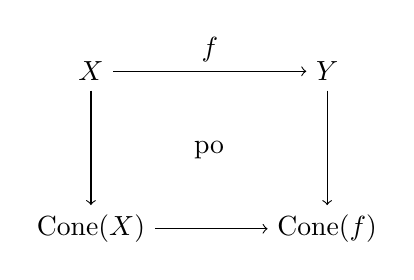
\begin{tikzpicture}
                \node (X) at (0, 0) {$X$};
                \node (Y) at (3, 0) {$Y$};
                \node (coneX) at (0, -2) {$\mathrm{Cone}(X)$};
                \node (conef) at (3, -2) {$\mathrm{Cone}(f)$};
                \node at (1.5, -1) {po};
                \draw[->] (X) -- node[above]{$f$} (Y);
                \draw[->] (X) -- (coneX);
                \draw[->] (Y) -- (conef);
                \draw[->] (coneX) -- (conef);
            \end{tikzpicture}
        \end{gather*}
    \end{remark}

\subsection{\difficult{Rational homotopy theory}}

    For the theory on differential graded algebras, see Chapter \ref{chapter:hda}.

    \newdef{Rational space}{\index{rational!space}
        A simply connected topological space $X$ for which the homotopy groups $\pi_n(X)$ are rational vector spaces.
    }

    \newdef{Rational homotopy equivalence}{\index{rational!homotopy equivalence}
        A continuous function $f:X\rightarrow Y$ for which the induced maps on rational homotopy groups
        \begin{gather}
            \pi_n(f)\otimes\mathbb{Q}:\pi_n(X)\otimes\mathbb{Q}\rightarrow\pi_n(Y)\otimes\mathbb{Q}
        \end{gather}
        are isomorphisms for all $n\in\mathbb{N}$. An equivalent requirement is that the induced map on rational (co)homology is an isomorphism (see the section on singular homology below).
    }

    \newdef{Rational homotopy category}{
        Consider the category \textbf{Top} of topological spaces. The rational homotopy category is obtained as the localization \ref{model:localization} of \textbf{Top} with respect to the collection of rational homotopy equivalences.
    }

    \newdef{Polynomial differential forms}{
        Consider the standard $n$-simplex $\Delta^n$ (Definition \ref{topology:simplex}). On this topological space one can define differential forms analogous to those from Section \ref{section:forms}. Let $\{t_i\}_{0\leq i\leq n}$ be $n+1$ generators in degree 0 (the barycentric coordinates). Together with $n+1$ associated generators $dt_i$ in degree 1, one can construct the free GCA over $\mathbb{Q}$. To preserve the geometric structure of $\Delta^n$ one has to quotient out the following relations:
        \begin{gather}
            \sum_{i=0}^n t_i = 1\qquad\text{and}\qquad\sum_{i=0}^n dt_i = 0.
        \end{gather}
        The resulting graded algebra is denoted by $\Omega^\bullet_{\text{poly}}(\Delta^n)$. In degree 0 this complex can be identified with the space of polynomial functions on $\Delta^n$. The ordinary differential forms can be obtained by taking the tensor product of $\Omega^\bullet_{\text{poly}}$ with the space of smooth functions on $\Delta^n$. Under this isomorphism the generators $dt_i$ are identified with the de Rham differentials of the barycentric coordinates.

        Morphisms $f:[m]\rightarrow[n]$ in the simplex category $\Delta$ induce morphisms of simplices and these in turn induce morphisms $F:\Omega^\bullet_{\text{poly}}(\Delta^n)\rightarrow\Omega^\bullet_{\text{poly}}(\Delta^m)$ defined by the following action on generators:
        \begin{gather}
            F(t_i) := \sum_{f(j)=i}t_j.
        \end{gather}
        It can be seen that this turns the above construction into a functor $\func{\Omega^\bullet_{\text{poly}}}{\Delta^{op}}{dgcAlg}$. By passing to the opposite functor and taking a left Kan extension along the Yoneda embedding $\Delta\hookrightarrow\mathbf{sSet}$, one obtains a functor $\func{\Omega^\bullet_{\text{poly}}}{sSet}{dgcAlg^{op}}$. Composition with the singular set functor $\func{\text{Sing}}{Top}{sSet}$ gives the \textbf{piecewise-polynomial differential forms} functor $\Omega^\bullet_{\text{pwpoly}}$.
    }

    \newdef{Relative Sullivan algebra}{\index{Sullivan!algebra}\label{topology:sullivan_algebra}
        An inclusion of DGCAs of the form \[(A,d)\hookrightarrow(A\otimes\Lambda^\bullet V,d'),\] where $A$ is any DGCA and $V$ is a $\mathbb{N}_0$-graded vector space such that:
        \begin{itemize}
            \item there is a well-ordered set $I$ indexing a linear basis $\{e_i\}_{i\in I}$ of $V$.
            \item for all $k\in I$ and all $e_k$ one has that
            \begin{gather}
                d'e_k\in A\otimes\Lambda^\bullet V(<k),
            \end{gather}
            where $V(<k):=\text{span}\{e_i\}_{i<k}$.
        \end{itemize}
        If in addition the implication
        \begin{gather}
            i<j\implies\deg(e_i)\leq\deg(e_j)
        \end{gather}
        holds for all $i,j\in I$, the relative Sullivan algebra is said to be \textbf{minimal}.

        If the Sullivan algebra is defined relative to the tensor unit $(k,0)$, where $k$ is the underlying field, it is just called a \textbf{Sullivan algebra}.
    }
    \begin{remark}
        The minimality condition admits an (equivalent) reformulation:
        \begin{gather}
            dV\subseteq A_{\geq1}\otimes\Lambda^\bullet V + A\otimes\Lambda^{\geq2}V.
        \end{gather}
    \end{remark}

    \begin{example}\label{topology:sullivan_algebras_specific}
        Consider the free DGCA $\Lambda(V)$ on a graded vector space $V$ of finite type with $V_0=V_1=0$. Then $(\Lambda(V),d)$ is a Sullivan algebra.
    \end{example}

    \newdef{Sullivan model}{\index{Sullivan!model}
        Let $X$ be a simply-connected topological space. A (minimal) Sullivan model for $X$ is a (minimal) Sullivan algebra equipped with a quasi-isomorphism to the DGA of piecewise-polynomial differential forms on $X$.
    }
    \begin{property}
        Minimal Sullivan models are unique up to isomorphism.
    \end{property}

    There is also another approach due to \textit{Quillen}. Instead of working with differential graded algebras, \textit{Quillen} used differential graded Lie algebras, i.e. strict $L_\infty$-algebras (Section \ref{section:higher_lie_structures}).
    \begin{construct}[Sketch, Quillen]
        To every simply-connected topological space $X$ one can associated a differential graded Lie algebra $L_\bullet(X)$ such that the homology of this complex is isomorphic to the (shifted) rational homotopy complex $\pi_{\bullet+1}(X)\otimes\mathbb{Q}$ of $X$.
    \end{construct}

\subsection{\difficult{Equivariant homotopy theory}}

    In this section topological spaces equipped with an action of a topological group $G$ will be considered (the group will often be a compact Lie group). Some notions will be defined very similarly to those in the previous section, but some others will look very differently.

    \newnot{Fixed-point space}{\index{fixed point}
        Consider a topological $G$-space $X$. The set of all its fixed points is denoted by $X^G$.
    }

    \newdef{Equivariant homotopy equivalence}{\index{homotopy!equivalence}
        A continuous function that is both an equivariant function and a homotopy equivalence in the ordinary sense.
    }
    \newdef{Weak equivariant homotopy equivalence}{
        An equivariant continuous function that restricts to an ordinary weak equivalence between the fixed-point subspaces for all closed subgroups $H\subset G$.
    }

    \begin{theorem}[Whitehead\footnotemark]\index{Whitehead}
        \footnotetext{This equivariant version of Theorem \ref{topology:whitehead} is due to \textit{Bredon}.}
        A continuous function between $G$-CW complexes is a weak equivariant homotopy equivalence if and only if it is a equivariant homotopy equivalence.
    \end{theorem}

    \newdef{Orbit category}{
        Let $G$ be a topological group. The orbit category $\mathbf{Orb}_G$ is the category defined by the following data:
        \begin{enumerate}
            \item the coset spaces $G/H$ with $H\subset G$ a closed subgroup as objects, and
            \item the equivariant homomorphisms as morphisms.
        \end{enumerate}
    }
    \begin{theorem}[Elmendorf]\index{Elmendorf}\index{orbit!category}
        The map $(X,H)\mapsto X^H$ sending a $G$-space to its fixed-point spaces can be interpreted as a functor $X:\mathbf{Orb}_G^{op}\rightarrow\mathbf{Top}$ or, equivalently, as a $\mathbf{Top}$-valued presheaf on the orbit category. By taking this a step further, one obtains a functor sending every topological space $X$ to such a presheaf.\footnote{This is the restriction of the Yoneda embedding to the subcategory $\mathbf{Orb}_G$ of $G\mathbf{Top}$.} To study the homotopy theory on these categories, one needs a choice of weak equivalences. Similar to the model structure on $\mathbf{sSet}$, one can choose the weak equivalences on $\mathbf{Psh}(\mathbf{Orb}_G)$ to be the levelwise weak equivalences. This gives an $(\infty,1)$-equivalence
        \begin{gather}
            \mathbf{Ho}(G\mathbf{Top})\cong\mathbf{Psh}(\mathbf{Orb}_G).
        \end{gather}
    \end{theorem}

    ?? COMPLETE ??

\section{Simplicial homology}\label{section:homology}
\subsection{Simplices}

    \newdef{Simplex}{\index{simplex}\index{vertex}\label{topology:simplex}
        A $k$-simplex $\sigma^k\equiv[t_0,\ldots,t_k]$ is defined as the following set:
        \begin{gather}
            \sigma^k := \left\{\sum_{i=0}^k\lambda_it_i\,\middle\vert\,\sum_{i=0}^k\lambda_i = 1\text{ and }\lambda_i\geq0\right\}.
        \end{gather}
        where the \textbf{vertices} $t_i\in\mathbb{R}^n$ are \textbf{affinely independent}, i.e. the vectors $t_i-t_0$ are linearly independent. Equivalently, a simplicial $k$-simplex  is the convex hull of the $k+1$ vertices $\{t_0,\ldots,t_k\}$.
    }
    \begin{remark}[Barycentric coordinates]\index{barycenter}
        The numbers $\lambda_i$ from the previous definition are called barycentric coordinates. This terminology stems from the fact that the point $\sum_{i=0}^k\lambda_it_i$ represents the \textit{barycenter} of a gravitational system consisting of masses $\lambda_i$ placed at the points $t_i$.
    \end{remark}
    \begin{example}[Standard simplex]\index{simplex!standard}\label{topology:standard_simplex}
        \begin{gather}
            \Delta^k := \left\{(x_0,\ldots,x_k)\in\mathbb{R}^{k+1}\,\middle\vert\,\sum_ix_i = 1 \text{ and }x_i\geq0\right\}
        \end{gather}
    \end{example}

    \newnot{Face}{\index{face}
        Consider a $k$-simplex $[v_0,\ldots,v_k]$. The \textbf{face} opposite to the vertex $v_i$ is the $(k-1)$-simplex $[v_0,\ldots,\widehat{v}_i,\ldots,v_k]$ obtained by removing the vertex $v_i$.
    }

    \newdef{Simplicial complex}{\index{simplicial!complex}
        A simplicial complex $\mathcal{K}$ is a set of simplices satisfying the following conditions:
        \begin{itemize}
            \item If $\sigma$ is a simplex in $\mathcal{K}$, so are its faces.
            \item If $\sigma_1,\sigma_2\in\mathcal{K}$, either $\sigma_1\cap\sigma_2 = \emptyset$ or $\sigma_1\cap\sigma_2$ is a face of both $\sigma_1$ and $\sigma_2$.
        \end{itemize}
        A simplicial $k$-complex is a simplicial complex where every simplex has dimension at most $k$.
    }

    \newdef{Path-connected complex}{\index{path!connected}
        A simplicial complex is said to be path-connected if every two vertices in are connected by an edge in.
    }

    \newdef{Polyhedron}{\index{polyhedron}
        Consider a simplicial complex. The polyhedron associated with it is the topological space constructed by equipping the complex with the Euclidean subspace topology.
    }

    \newdef{Triangulable spaces}{\index{triangulation}
        Let $X$ be a topological space and let $\mathcal{K}$ be a polyhedron. If there exists a homeomorphism $\varphi:\mathcal{K}\rightarrow X$, then $X$ is said to be triangulable and $\mathcal{K}$ is called a \textbf{triangulation} of $X$.
    }
    \begin{property}[Fundamental group]
        Let $\mathcal{K}$ be a path-connected polyhedron with basepoint $a_0$ and consider a contractible one-dimensional subpolyhedron $\mathcal{C}\subset\mathcal{K}$ containing all vertices of $\mathcal{K}$. Let $G$ be the free group \ref{group:free_group} with generators $g_{ij}$ corresponding to the ordered 1-simplices $[v_i,v_j]\in\mathcal{K}$. On this group one can define the following relations:
        \begin{itemize}
            \item $g_{ij} = e$ if $[v_i,v_j]\in\mathcal{C}$.
            \item $g_{ij}g_{jk} = g_{ik}$ for every ordered 2-simplex $[v_i,v_j,v_k]\in\mathcal{K}\backslash\mathcal{C}$.
        \end{itemize}
        The quotient group of $G$ by these relations is isomorphic to the fundamental group $\pi_1(\mathcal{K},a_0)$.
    \end{property}
    \begin{result}
        Property \ref{topology:homeomorphic_homotopy}, which states that homeomorphic spaces have the same homotopy groups, implies that the fundamental group of a triangulable space can be computed by looking at its triangulations.
    \end{result}

\subsection{Simplicial homology}

    \newdef{Chain group}{\index{chain!group}\label{topology:chain_group}
        Let $\mathcal{K}$ be a simplicial $n$-complex. The $k^{th}$ chain group $C_k(\mathcal{K})$ is defined as the free Abelian group generated by the $k$-simplices in $\mathcal{K}$:
        \begin{gather}
            C_k(\mathcal{K}) := \left\{\sum_ia_i\sigma_i\,\middle\vert\,\sigma_i\text{ is a $k$-simplex in $\mathcal{K}$}, a_i\in\mathbb{Z}\right\}.
        \end{gather}
        For $k>n$ and $k<0$, $C_k(\mathcal{K})$ is defined to be $\{0\}$.
    }

    \newdef{Boundary operator}{\index{boundary}
        The boundary operator $\partial_k:C_k(\mathcal{K})\rightarrow C_{k-1}(\mathcal{K})$ is the group morphism defined by the following properties:
        \begin{itemize}
            \item\textbf{Linearity}:
                \begin{gather}
                    \partial_k\left(\sum_ia_i\sigma_i\right) = \sum_ia_i\partial_k\sigma_i,
                \end{gather}
            \item\textbf{Action on generators}
                \begin{align}
                    \partial_k[v_0,\ldots,v_k] &= \sum_{i=0}^k(-1)^i[v_0,\ldots,\hat{v}_i,\ldots,v_k],\\
                    \partial_0[v] &= 0.
                \end{align}
        \end{itemize}
    }

    \begin{property}[Chain condition]\label{topology:boundary_operator_relation}
        The boundary operators satisfy the following relation:
        \begin{gather}
            \partial_k\circ\partial_{k+1} = 0.
        \end{gather}
        This property turns the system $(C_k,\partial_k)$ into a chain complex \ref{homalg:chain_complex}.
    \end{property}

    \newdef{Cycle group}{\index{cycle}
        The $k^{th}$ cycle group $Z_k(\mathcal{K})$ is defined as the set of $k$-chains $\sigma_k$ such that $\partial_k\sigma_k = 0$. These chains are called \textbf{cycles}.
    }
    \newdef{Boundary group}{
        The $k^{th}$ boundary group $B_k(\mathcal{K})$ is defined as the set of $k$-chains $\sigma_k$ for which there exists a $(k+1)$-chain $N$ such that $\partial_{k+1}N = \sigma_k$. These chains are called \textbf{boundaries}.
    }
    \newdef{Homology group}{\index{homology!simplicial}
        From Property \ref{topology:boundary_operator_relation} it follows that $B_k(\mathcal{K})\subset Z_k(\mathcal{K})$ is a subgroup. One can thus define the $k^{th}$ homology group $H_k(\mathcal{K})$ as the following quotient group:
        \begin{gather}
            H_k(\mathcal{K}) := Z_k(\mathcal{K})/B_k(\mathcal{K}).
        \end{gather}
        Theorem \ref{group:theorem:free_group} says that $H_k(\mathcal{K})$ can be written as $G_k\oplus T_k$. Both of these groups say something about $\mathcal{K}$. The rank of $G_k$, denoted by $R_k(\mathcal{K})$, is equal to the number of $(k+1)$-dimensional holes in $\mathcal{K}$. The torsion subgroup $T_k$ says how the space $\mathcal{K}$ is ``twisted''.
    }

    \newdef{Betti numbers}{\index{Betti number}
        The ranks $R_k(\mathcal{K})$ are called the Betti numbers of $\mathcal{K}$.
    }
    \begin{definition}[Euler characteristic]\index{Euler!characteristic}\index{Euler-Poincar\'e formula}\label{topology:euler_characteristic}
        The Euler characteristic of a triangulable space $X$ is defined as follows:
        \begin{gather}
            \chi(X) := \sum_i(-1)^iR_i(X).
        \end{gather}
        This formula is sometimes called the \textbf{Poincar\'e} or \textbf{Euler-Poincar\'e} formula.
    \end{definition}

    \begin{property}[Isomorphisms]
        If two topological spaces have the same homotopy type, in particular when they are homeomorphic, they have isomorphic homology groups.
    \end{property}
    \begin{result}
        As was the case for the fundamental group, it follows from the definition of a triangulation that one can study the homology groups of a given triangulable space by looking at its triangulations.
    \end{result}

    Although the homology invariants do not depend on the choice of triangulation, a remark about the existence of nonequivalent triangulations should be given.
    \begin{remark}[Hauptvermutung $\clubsuit$]
        Before the construction of a counterexample it was believed (hence the terms \textit{Hauptvermutung} in German or \textit{main conjecture} in English) that every two triangulations of a topological space allowed a common refinement and, hence, where equivalent for many constructions. However, it was shown that this conjecture is generally false, e.g. for topological manifolds in dimensions 5 and higher there exist an infinite number of nonequivalent triangulations. In dimensions up to 4 it was proven by Rad\'o and Moise that the Hauptvermutung holds for all topological manifolds (see also Theorem \ref{diff:rado_moise}).
    \end{remark}

    \begin{construct}
        The definition of homology groups can be generalized by letting the (formal) linear combinations used in the definition of the chain group be of the following form:
        \begin{gather}
            c = \sum_ig_i\sigma_i^k,
        \end{gather}
        where $g_i\in G$ for some Abelian group $G$. The $k^{th}$ homology group of $X$ with coefficients in $G$ is denoted by $H_k(X;G)$.
    \end{construct}
    \begin{property}[Vanishing torsion]
        When $G$ is a field, such as $\mathbb{Q}$ or $\mathbb{R}$, the torsion subgroups $T_k$ vanish. The relation between integral homology and homology with coefficients in a group is given by the \textit{universal coefficient theorem}.
    \end{property}

    \newformula{K\"unneth formula}{\index{K\"unneth formula}
        Let $X,Y$ be two simplicial complexes. The homology groups of the Cartesian product $X\times Y$ with coefficients in a field $F$ is given by
        \begin{gather}
            H_k(X\times Y;F) = \bigoplus_{k=i+j}H_i(X;F)\otimes H_j(Y;F).
        \end{gather}
        When the requirement of $F$ being a field is relaxed to it merely being a group, the torsion subgroups have to be taken into account. See the literature for this general form.
    }

\subsection{Relative homology}

    In this section the homology of a simplicial complex $K$ ``modulo'' a subcomplex $L$ is considered.

    \newdef{Relative chain group}{\index{chain}
        The $k$-chain group of $K$ modulo $L$ is defined as the following quotient group:
        \begin{gather}
            C_k(K,L) := C_k(K)/C_k(L).
        \end{gather}
        Equivalence classes will be denoted by square brackets $[c]$, where $c\in C_\bullet(K)$.
    }
    \newdef{Relative boundary operator}{\index{boundary}
        The relative boundary operator $\overline\partial_k$ is defined as follows:
        \begin{gather}
            \overline\partial_k[c_k] := [\partial_kc_k],
        \end{gather}
        where $\partial_k$ on the right-hand side denotes the boundary operator in ordinary homology. This is a well-defined operation since $\partial C_\bullet(L)\subseteq C_\bullet(L)$.
    }
    \newdef{Relative homology groups}{\index{homology!relative}
        The relative cycle and relative boundary groups are defined analogous to their ordinary counterparts. The relative homology groups are defined as follows:
        \begin{gather}
            H_k(K,L) := \stylefrac{\ker(\overline\partial_k)}{\im(\overline\partial_{k+1})}.
        \end{gather}
        Elements $h_k\in H_k(K,L)$ can be represented as $h_k=z_k + C_k(L)$ such that $\partial_kz_k\in C_{k-1}(L)$.
    }

    \begin{property}[Homotopy invariance]
        Consider two topological spaces $X,Y$ with subspaces $A\subset X,B\subset Y$. If a continuous function $f:X\rightarrow Y$ is a homotopy equivalence such that the restriction to $A$ gives a homotopy equivalence $f|_A:A\rightarrow B$, the relative homology complexes $H_\bullet(X,A)$ and $H_\bullet(Y,B)$ are isomorphic.
    \end{property}

    \begin{property}[Long sequence for a pair]
        The relative homology groups fit in the following (long) exact sequence:
        \begin{gather}
            \cdots\longrightarrow H_k(L)\overset{i_\ast}{\longrightarrow}H_k(K)\overset{j_\ast}{\longrightarrow}H_k(K,L)\overset{\partial_k}{\longrightarrow}H_{k-1}(L)\longrightarrow\cdots,
        \end{gather}
        where $i_\ast$ and $j_\ast$ are the homology morphisms induced by the inclusions $i:L\rightarrow K$ and $j:K\rightarrow(K,L)$.
    \end{property}

    \begin{theorem}[Excision theorem]\index{excision}\label{topology:excision_theorem}
        Let $U,V$ and $X$ be simplicial complexes such that $U\subset V\subset X$. If the closure $\overline{U}$ is contained in the interior $V\degree$, then
        \begin{gather}
            H_k(X,V) \cong H_k(X\backslash U,V\backslash U).
        \end{gather}
    \end{theorem}

    \newdef{Reduced homology}{\index{homology!reduced}
        Consider the chain complex $C_\bullet(X)$. Example \ref{topology:point_homology} says that a point $\{\ast\}$ has homology $\mathbb{Z}$ concentrated in degree $0$. However, it would be nice if the point $\ast$ had vanishing homology. To this end one can augment \ref{homalg:resolution} the chain complex $C_\bullet(X)$ of any topological space by the group $\mathbb{Z}$ to obtain the reduced homology complex $\widetilde{H}_\bullet(X)$:
        \begin{gather}
            H_n(X) \cong
            \begin{cases}
                \widetilde{H}_0(X)\oplus\mathbb{Z}&n=0\\
                \widetilde{H}_n(X)&n\neq0.
            \end{cases}
        \end{gather}
    }
    \begin{property}
        Consider a pointed topological space $(X,x_0)$. The reduced homology $\widetilde{H}_\bullet(X)$ is isomorphic to the relative homology $H_\bullet(X,\{x_0\})$.
    \end{property}

    \begin{property}[Good pair]\index{NDR pair}\label{topology:ndr_pair_homology}
        \nomenclature[A_NDR]{NDR}{neighbourhood deformation retract}
        Consider a topological space $X$ together with a subspace $A$. The pair $(X,A)$ is called a \textbf{neighbourhood deformation retract (NDR) pair}\footnote{Some people call this a \textbf{good pair}, while others define an NDR pair more restrictively.} if there exists a neighbourhood $V\subset X$ of $A$ such that $V$ deformation retracts onto $A$. Equivalently, the inclusion $A\subset X$ is a closed cofibration \ref{topology:cofibration}.

        Given an NDR pair $(X,A)$, there exists an isomorphism
        \begin{gather}
            H_\bullet(X,A)\cong\widetilde{H}_\bullet(X/A).
        \end{gather}
    \end{property}

\subsection{Examples}

    \begin{example}\label{topology:point_homology}
        Let $X$ be a contractible space.
        \begin{gather}
            H_k(X) =
            \begin{cases}
                \mathbb{Z}&k=0\\
                0&\text{otherwise}
            \end{cases}
        \end{gather}
    \end{example}
    \begin{example}
        Let $P$ be a path-connected simplicial complex.
        \begin{gather}
            H_0(P) = \mathbb{Z}
        \end{gather}
        Furthermore, every point $p\in P$ determines a generator $\langle p \rangle\in H_0(P)$.
    \end{example}

    \begin{example}
        The homology groups of the $n$-sphere $S^n$ are given by
        \begin{gather}
            H_k(S^n)=
            \begin{cases}
                \mathbb{Z}&k=0\text{ or }k=n\\
                0&\text{otherwise}.
            \end{cases}
        \end{gather}
    \end{example}

    \newdef{Homology sphere}{\index{homology!sphere}
        A $n$-dimensional manifold having the same homology groups as the $n$-sphere.
    }
    \newdef{Degree}{\index{degree!of map}\label{topology:degree}
        The example above says that $H_n(S^n)=\mathbb{Z}$. Given a map $f:S^n\rightarrow S^n$, the induced map $f_*$ on homology is an endomorphism of $\mathbb{Z}$ and, hence, is of the form $f(x)=dx$ where $d\in\mathbb{Z}$. This coefficient is called the degree of $f$.
    }
    \begin{property}
        Two maps $f:S^n\rightarrow S^n$ have the same degree if and only if they are homotopic.
    \end{property}

    \begin{example}
        Consider the closed (or open) disks $D_n$.
        \begin{gather}
            H_k(D_n,\partial D_n) =
            \begin{cases}
                \mathbb{Z}&k=n\\
                0&\text{otherwise}
            \end{cases}
        \end{gather}
        This holds for any $n$-skeleton $X^n$ of a CW-complex.
    \end{example}

\section{Singular homology}\label{section:singular_homology}

    \newdef{Singular simplex}{\index{simplex!singular}
        Recall the \textbf{standard} $k$-simplex $\Delta^k$ from Example \ref{topology:standard_simplex}. A singular $k$-simplex in a topological space $X$ is defined as a continuous function $\sigma:\Delta^k\rightarrow X$.
    }
    \sremark{The name singular comes from the fact that the function $\sigma$ need not be injective.}

    \newdef{$\Delta$-complex}{\index{$\Delta$-complex}
        Let $\{\sigma_i:\Delta^n\rightarrow X\}_{i\in I}$ be a collection of singular simplices in $X$, where the dimension $n$ may depend on the index $i\in I$. This collection forms a $\Delta$-complex on $X$ if it satisfies the following conditions:
        \begin{itemize}
            \item The restrictions $\sigma_i|_{\overset{\circ}{\Delta}{}^n}$ are injective and every point in $X$ lies in the image of exactly one such restriction.
            \item The restriction of a simplex $\sigma_i$ to any one of the faces of $\Delta^n$ is equal to some other $\sigma_j$.
            \item A set in $X$ is open if and only if it all of its inverse images $\sigma_i^{-1}$ are open.
        \end{itemize}

        Similar to a CW-complex or \textit{cellular complex}, these conditions imply that every $\Delta$-complex can be constructed inductively from a (discrete) set of vertices by gluing and identifying edges.
    }

    \newdef{Singular chain group}{\index{chain}
        The singular chain group $S_k(X)$ with coefficients in a group $G$ is defined as the set of formal linear combinations $\sum_ig_i\sigma_i$, where the $\sigma_i$ are singular $k$-simplices in $X$. The basis of this free group is in most cases infinite as there are in general many ways to map $\Delta^k$ to $X$.
    }

    Before continuing, one first need to introduce an important concept in the context of simplicial objects:
    \newdef{Face map}{\index{face!map}
        The face maps are morphisms $\varepsilon_i^k:\Delta^{k-1}\rightarrow\Delta^k$ that map $\Delta^{k-1}$ onto the $i^{th}$ face of $\Delta^k$. They are explicitly given by
        \begin{gather}
            \varepsilon_i^k(s_0,\ldots,s_{k-1}) := (s_0,\ldots,s_{i-1},0,s_i,\ldots,s_{k-1}).
        \end{gather}
        Their defining property is the following relation:
        \begin{gather}
            \varepsilon_i^k\circ\varepsilon_j^{k-1} = \varepsilon_j^k\circ\varepsilon_{i-1}^{k-1},
        \end{gather}
        where $j\leq i$.
    }
    \sremark{Some authors (for example the authors at nLab) call these maps \textit{degeneracy maps} and call what in these notes are called \textit{degeneracy maps} face maps. This is a consequence of working in a dual picture (they work in the opposite of the simplex category $\simplex$).}

    \newdef{Singular boundary operator}{\index{face!map}
        The singular boundary operator $\partial$ (the same notation as for simplicial boundary operators is used for simplicity) is defined by its linear action on the singular chain groups $S_k(X;G)$. It follows that it is uniquely defined by its action on the singular $k$-simplices $\sigma^k$.

        The action of the boundary operator on the singular $k$-simplex $\sigma^k$ is given by
        \begin{gather}
            \partial_k\sigma^k = \sum_{i=0}^k(-1)^i\sigma^k\circ\varepsilon^k_i,
        \end{gather}
        where the $\varepsilon^k_i$ are the face maps defined above. The singular boundary operators satisfy the same relation as the the simplicial boundary operators:
        \begin{gather}
            \partial_{k-1}\circ\partial_k = 0.
        \end{gather}
        It follows that $S_k(X;G)$ is also a chain complex.
    }

    \newdef{Singular homology group}{\index{homology!singular}
        The singular homology groups of a topological space with coefficients in an Abelian group $G$ are defined as follows:
        \begin{gather}
            H_k(X;G) := \frac{\ker(\partial_k)}{\im(\partial_{k+1})}.
        \end{gather}
    }
    \begin{property}[Simplicial homology]
        For triangulable spaces singular homology is isomorphic to simplicial homology. When $X$ is not triangulable, this property is not valid. The singular approach to homology is strictly more general, but it is often more difficult to compute (even in the case of triangulable spaces).
    \end{property}

    \begin{property}[Induced morphism]\index{pushforward}\label{topology:pushforward}
        Consider a continuous function $f:X\rightarrow Y$ between topological spaces. This induces a morphism $f_*:S_k(X;G)\rightarrow S_k(Y;G)$ on the chain groups as follows:
        \begin{gather}
            f_*\left(\sum_\sigma c_\sigma\sigma\right) := \sum_\sigma c_\sigma f\circ\sigma.
        \end{gather}
        This map takes cycle (resp. boundary) groups to (subgroups of) cycle (resp. boundary) groups and, hence, induces a morphism of homology groups, called the \textbf{pushforward}:
        \begin{gather}
            f_\ast:H_k(X)\rightarrow H_k(Y):\langle h \rangle\mapsto\langle f_*(h)\rangle.
        \end{gather}
    \end{property}
    \begin{result}
        $H_k$ is a functor $\mathbf{Top}\rightarrow\mathbf{Ab}$ that maps topological spaces to their homology groups and continuous functions $f$ to their pushforwards $f_\ast$.
    \end{result}

    \begin{theorem}[Hurewicz]\index{Hurewicz}
        Let $X$ be path-connected and let $[\cdot]$ and $\langle\cdot\rangle$ denote the equivalence classes in the homotopy and homology groups, respectively. Because every path can be obtained as a singular 1-chain, the map $h:\pi(X)\rightarrow H_1(X):[\gamma]\mapsto\langle\gamma\rangle$ defines a group morphism. Furthermore, this map induces an isomorphism $h':\pi(X)/[\pi(X), \pi(X)]\rightarrow H_1(X)$.

        More generally, for every topological space $X$ and every $n\in\mathbb{N}$ there exists a morphism $h_*:\pi_n(X)\rightarrow H_n(X)$. If $Y$ is $(n-1)$-connected, then for every $k\leq n$ this morphism is in fact an isomorphism.
    \end{theorem}

    \newdef{Singular cohomology}{\index{cohomology}\index{pullback}
        The singular cohomology groups of a topological space $X$ with coefficients in an Abelian group $G$ are defined as follows:
        \begin{gather}
            H^k(X;G) := \hom(H_k(X),G),
        \end{gather}
        where on the right-hand side the integral (singular) homology of $X$ is used. A continuous function $f:X\rightarrow Y$ induces a \textbf{pullback} morphism $f^*:H^\bullet(Y;G)\rightarrow H^\bullet(X;G)$ on cohomology by duality:
        \begin{gather}
            f^*g(\sigma) := g(f_*\sigma),
        \end{gather}
        where $f_*$ is the pushforward \ref{topology:pushforward} induced by $f$.
    }
    \begin{property}[Representability]
        Let $X$ be a CW complex. There exists an isomorphism
        \begin{gather}
            [X,K(G,n)]\rightarrow H^n(X;G)
        \end{gather}
        between the homotopy classes of maps $X\rightarrow K(G,n)$ and the $n^{th}$ singular cohomology of $X$ with coefficients in $G$. (This result can be widely generalized cf. Theorem \ref{topology:brown} further below.)

        \begin{proof}
            Consider the Eilenberg-Maclane space $K(G,n)$ for $G$ (Definition \ref{topology:eilenberg_maclane}). By the Hurewicz theorem there exists an isomorphism $H_n(K(G,n))\cong\pi_n(K(G,n))\cong G$. By definition of cohomology $H^n(K(G,n);G)=\hom(H_n(K(G,n)),G)$ and thus $H^n(K(G,n);G)\cong\hom(G,G)$. In particular, there corresponds a cohomology class $\psi$ to the identity mapping on $G$. The cohomology class in $H^n(X;G)$ associated to a homotopy class of functions $f:X\rightarrow K(G,n)$ is given by $f^*\psi$.
        \end{proof}
    \end{property}

\section{\difficult{Axiomatic approach}}

    \newdef{Eilenberg-Steenrod axioms}{\index{Eilenberg-Steenrod axioms}\label{topology:eilenberg_steenrod_axioms}
        All (co)homology theories have a set of properties in common. By treating these properties as axioms, one can construct relative (co)homology theories as a sequence of functors $H_k:\mathbf{Top}\times\mathbf{Top}\rightarrow\mathbf{Ab}$ (technically one should replace $\mathbf{Top}\times\mathbf{Top}$ by the category consisting of subspace inclusions $A\hookrightarrow X$). The axioms are as follows:
        \begin{enumerate}
            \item\textbf{Homotopy invariance}: If $f,g$ are homotopic maps, their induced homology maps are the same: \[f\cong g\implies\forall k\in\mathbb{N}:H_k(f) = H_k(g).\]
            \item\textbf{Excision}: If $U\subset V\subset X$ and $\overline U\subset V\degree$, then $H_k(X,V)\cong H_k(X\backslash U,V\backslash U)$.
            \item\textbf{Additivity}: If $X = \bigsqcup_i X_i$, then $H_k(X)\cong\bigoplus_i H_k(X_i)$.
            \item\textbf{Exactness}: Each pair $(X,A)$, where $A\subset X$, induces a long exact sequence
            \begin{gather}
                \cdots\longrightarrow H_k(A)\overset{i_\ast}{\longrightarrow}H_k(X)\overset{j_\ast}{\longrightarrow}H_k(X,A)\overset{\partial_k}{\longrightarrow}H_{k-1}(A)\longrightarrow\cdots,
            \end{gather}
            where $i_\ast$ and $j_\ast$ are the pushforwards of the inclusions $i:A\rightarrow X$ and $j:X\rightarrow(X,A)$.
            \item\textbf{Dimension}: If $X$ is a singleton, then $H_k(X) = \{0\}$ for all $k\geq1$. The group $H_0(X)$ is called the \textbf{coefficient group} and gives the coefficients used in the linear combinations of the chain group.
        \end{enumerate}
    }
    \begin{remark}
        If the dimension axiom is removed from the set of axioms, the so-called \textit{extraordinary (or generalized) homology theories} are obtained.
    \end{remark}

    Although the following theorem sounds like more of a purely category-theoretic statement, its main application is the definition of cohomology theories:
    \begin{theorem}[Brown's representability theorem]\index{Brown's representability theorem}\index{Mayer-Vietoris}\label{topology:brown}
        Consider a presheaf $H$ on the homotopy category of pointed connected topological spaces $\mathbf{Ho}(\mathbf{Top}^{con}_*)$. This functor is representable if and only if it satisfies the following conditions:
        \begin{itemize}
            \item It maps coproducts to products.
            \item It maps weak pushouts to weak pullbacks. (Weak pushouts in the homotopy category $\mathbf{Ho}(\mathbf{Top})$ come from homotopy pushouts in $\mathbf{Top}$.)
        \end{itemize}
    \end{theorem}
    \begin{remark}
        If one constructs the homotopy category using the CW-model structure in $\mathbf{Top}$, the second condition can be restated as a \textit{Mayer-Vietoris axiom}. Consider a CW complex $U$ and two subcomplexes $V_1,V_2$. If $x\in H(V_1),y\in H(V_2)$ and $x=y$ on the intersection $V_1\cap V_2$, there exists a $z\in H(U)$ that restricts to $x$ (resp. $y$) on $V_1$ (resp. $V_2$).
    \end{remark}
    \begin{result}[Cohomology]
        Every (generalized) cohomology theory is representable. Given cohomology functors $\{H^n\}_{n\in\mathbb{N}}$, there exists a sequence of pointed topological spaces $\seq{X}$ such that
        \begin{gather}
            H^n(Y) := [Y,X_n]
        \end{gather}
        for all $n\in\mathbb{N}$.
    \end{result}

    For reduced cohomology theories there exist suspension isomorphisms
    \begin{gather}
        \widetilde{H}^n(Y)\cong\widetilde{H}^{n+1}(\Sigma Y).
    \end{gather}
    Under Brown's theorem these induce isomorphisms $X_n\cong\Omega X_{n+1}$. This endows the sequence of spaces $\seq{X}$ with the following structure:
    \newdef{Spectrum\footnotemark}{\index{spectrum}\label{topology:spectrum}
        \footnotetext{Sometimes called an $\Omega$-spectrum to distinguish it from other (possibly more general) spectra.}
        A sequence of pointed topological spaces $\seq{X}$ such that $X_n\cong\Omega X_{n+1}$. (The isomorphism can be a weak homotopy equivalence or homeomorphism depending on the context.)
    }
    \begin{property}
        Brown's representability theorem shows that there exists a bijection between isomorphism classes of (generalized) cohomology theories and homotopy-equivalence classes of spectra.
    \end{property}

\section{Equivariant cohomology}\index{equivariant!cohomology}

    In this section topological spaces equipped with a continuous action of a topological group $G$ will be considered. These spaces will be called topological $G$-spaces or just $G$-spaces.

    \newdef{Equivariant cohomology}{\index{Borel!construction}\label{topology:equivariant_cohomology}
        Let $X$ be a topological $G$-space for which the $G$-action is free. The equivariant cohomology of $X$ is defined as
        \begin{gather}
            H_G^\bullet(X) := H^\bullet(X/G),
        \end{gather}
        where $X/G$ is the orbit space with respect to the action of $G$ on $X$.

        If the action is not free, a more general construction needs to be used. Consider the universal bundle $\pi:EG\rightarrow BG$ from Definition \ref{diff:classifying_space}. From this bundle one can construct the associated bundle $EG\times_G X$ (this is sometimes called the \textbf{Borel construction}). It gives a model for the homotopy quotient $X/\!\!/G$. The $G$-equivariant cohomology of $X$ is then defined as the singular cohomology of the Borel construction:
        \begin{gather}
            H_G^\bullet(X) := H^\bullet(EG\times_GX).
        \end{gather}
    }

    ?? COMPLETE (E.G. LECTURES OF TU ON YOUTUBE) ??
\chapter{Sheaf Theory}\label{chapter:sheaf}

    A reference aimed towards the study of differential geometry is \cite{brylinski}. For the concept of a sheaf in category theory, see Section \ref{section:grothendieck_topos}.

\section{Presheaves}

    \newdef{Presheaf}{\index{presheaf}\index{section}
        Let $(X,\tau)$ be a topological space. A presheaf on $X$ consists of a choice of algebraic structure $\mathcal{F}(U)$ for every open set $U\in\tau$ and a morphism $\Phi^U_V:\mathcal{F}(U)\rightarrow \mathcal{F}(V)$ for every two open sets $U,V\in\tau$ with $V\subseteq U$ such that the following conditions are satisfied:
        \begin{enumerate}
            \item $\Phi^U_U = \mathbbm{1}_{\mathcal{F}(U)}$, and
            \item $W\subseteq V\subseteq U\implies\Phi^U_W = \Phi^V_W\circ\Phi^U_V$.
        \end{enumerate}
        The set $\mathcal{F}(U)$ is called the set of \textbf{sections} over $U$ and the morphisms $\Phi^U_V$ are called the \textbf{restriction maps}.
    }
    \newdef{Morphism of presheaves}{\index{morphism!of presheaves}\index{germ}
        Let $\mathcal{F},\mathcal{F}'$ be two presheaves on a topological space $X$. A morphism $\mathcal{F}\rightarrow\mathcal{F}'$ is a set of morphisms $\Psi_U:\mathcal{F}(U)\rightarrow\mathcal{F}'(U)$ that commute with the restriction maps $\Phi^U_V$.
    }
    \begin{adefinition}[Categorical definition]
        Using the language of category theory one can give a more concise definition. Let $\mathbf{C}$ be a category and let $X$ be a topological space. A $\mathbf{C}$-valued presheaf on $X$ is a contravariant functor $\mathcal{F}:\mathbf{Open}(X)\rightarrow\mathbf{C}$. A morphism of presheaves is a natural transformation between such functors. As such the category of presheaves on a topological space $X$ is in fact the presheaf topos on $\mathbf{Open}(X)$.
    \end{adefinition}

    \begin{example}[Constant presheaf]\label{sheaf:constant_presheaf}
        Let $S$ be any set. The constant presheaf on $X$ with target $S$ is defined by
        \begin{gather}
            \mathcal{F}(U) := S
        \end{gather}
        for every open set $U\subseteq X$.
    \end{example}

\section{Sheaves}

    \newdef{Sheaf}{\index{sheaf}\label{sheaf:def}
        Let $(X,\tau)$ be a topological space. A sheaf on $X$ is a presheaf $\mathcal{F}$ satisfying the following conditions:
        \begin{enumerate}
            \item\textbf{Locality (or separation)}: Let $\{U_i\}_{i\in I}\subset\tau$ be an open cover of $U\subseteq X$ and consider sections $s,t\in\mathcal{F}(U)$. If $\forall i\in I:s|_{U_i}=t|_{U_i}$, then $s=t$. This is equivalent to saying that that $\mathcal{F}(U)$ injects into $\prod_i\mathcal{F}(U_i)$ for all open covers of $U$.
            \item\textbf{Gluing}: Let $\{U_i\}_{i\in I}\subset\tau$ be an open cover of $U\subseteq X$ and let $\{s_i\in\mathcal{F}(U_i)\}_{i\in I}$ be a collection of local sections. If $\forall i,j\in I:s_i|_{U_i\cap U_j} = s_j|_{U_i\cap U_j}$, there exists a section $s\in\mathcal{F}(U)$ such that $\forall i\in I:s|_{U_i} = s_i$.
        \end{enumerate}
    }
    \begin{remark}[Separated presheaves]
        If a global section exists by the gluing condition, it is automatically unique by the separation axiom. In some texts these two conditions are combined in a single gluing condition that requires a unique global section. Presheaves satisfying only the first condition are said to be \textbf{separated}. (See also the footnote in Definition \ref{topos:sheaf}.)
    \end{remark}

    \begin{notation}[Category of sheaves]
        \nomenclature[S_Sheaf]{$\mathbf{Sh}(X)$}{category of sheaves on a topological space $X$}
        Similar to the case of presheaves, one can define a morphism of sheaves as a collection of morphisms that commute with the restriction maps. The sheaves and sheaf morphisms on a space $X$ form a full subcategory of the category of presheaves, denoted by $\mathbf{Sh}(X)$.
    \end{notation}
    \begin{property}[\difficult{Sheaf topos}]
        The category of sheaves $\mathbf{Sh}(X)$ is in fact an elementary topos, called the sheaf topos on $X$. See Property \ref{topos:sheaf_topos}.
    \end{property}

    \begin{property}
        Let $X$ be a topological space and let $\mathcal{F}$ be a presheaf on $X$. $\mathcal{F}$ is a sheaf on $X$ if for any open $U\subseteq X$ and every open cover $\{U_i\}_{i\in I}$ of $U$ the following diagram is an equalizer diagram:
        \begin{gather}
            \label{sheaf:equalizer}
            \mathcal{F}(U)\rightarrow\prod_{i\in I}\mathcal{F}(U_i)\rightrightarrows\prod_{i, j\in I}\mathcal{F}(U_i\cap U_j).
        \end{gather}
        The two morphisms on the right are induced by the restriction morphisms $\Phi^{U_i}_{U_i\cap U_j}$ and $\Phi^{U_j}_{U_i\cap U_j}$.
    \end{property}

    \newdef{Stalk}{\index{stalk}\index{germ}
        Consider a point $x\in X$ together with the set of all neighbourhoods of $x$. This set can be turned into a directed set \ref{set:directed_set} by equipping it with the (partial) order relation \[U\geq V\implies U\subseteq V.\] This turns the sheaf $\mathcal{F}$ on $X$ into a directed system. The stalk at $x$ is defined as the following direct limit \ref{algebra:direct_limit}:
        \begin{gather}
            \mathcal{F}_x := \varinjlim_{U\ni x} \mathcal{F}(U).
        \end{gather}
        The equivalence class of a section $s\in\mathcal{F}(U)$ in $\mathcal{F}_x$ is called the \textbf{germ} of $s$ at $x$. Two sections belong to the same germ at $x$ if there exists a neighbourhood of $x$ on which they coincide.
    }
    \begin{notation}
        Similar to the notation of the restriction morphisms, the morphism that maps every section to its germ at $x$ is denoted by $\Phi^U_x$.
    \end{notation}

    \begin{property}
        Two subsheaves of a sheaf $\mathcal{F}$ on $X$ are equal if and only if their stalks are equal as subsets of $\mathcal{F}_x$ for all points $x\in X$. However, this does not imply that two sheaves with isomorphic stalks are equal (or even isomorphic)!
    \end{property}

    \begin{example}[Global sections functor]\index{global!sections}\label{sheaf:global_sections_functor}
        Let $X$ be a topological space. The global sections functor $\Gamma(X,-)$ is defined as the functor $\Gamma(X,-):\mathbf{Sh}(X)\rightarrow\mathbf{Set}:\mathcal{F}\rightarrow\mathcal{F}(X)$.
    \end{example}
    \begin{example}[Sheaf of sections]\index{sheaf!of sections}
        Consider a continuous function $f:X\rightarrow Y$. This function induces a sheaf on $Y$ in the following way:
        \begin{gather}
            \mathcal{F}(U) := \{s:U\rightarrow X\mid f\circ s=\mathbbm{1}_U\}.
        \end{gather}
        It is the sheaf that assigns to every open set the local sections of $f$ in the sense of Definition \ref{cat:retract}.
    \end{example}

    \begin{construct}[Associated sheaf]\index{sheafification}\index{section!continuous}
        Consider a presheaf $\mathcal{F}$ on a topological space $X$. From this presheaf one can construct a sheaf $\overline{\mathcal{F}}$, called the \textbf{sheafification} or associated sheaf of $\mathcal{F}$, in the following way. First, define $\overline{\mathcal{F}}$ as the a presheaf
        \begin{gather}
            \overline{\mathcal{F}}(U) := \left\{(s_x)_{x\in U}\in\prod_{x\in U}\mathcal{F}_x\,\middle\vert\,\forall x\in U:\exists\text{ open }V\ni x,t\in\mathcal{F}(V):\forall v\in V:s_v = \Phi^V_v(t)\right\}.
        \end{gather}
        Sections of this sheaf are said to be \textbf{continuous}. This statement can be made formal using the concept of an \'etal\'e space (see Construction \ref{sheaf:etale_construction} further on). The restriction maps $\rho^U_V$ are defined as follows:
        \begin{gather}
            \rho^U_V:(s_x)_{x\in U}\mapsto(s_x)_{x\in V}.
        \end{gather}
        It is easily proven that this presheaf is in fact a sheaf, the sheafification of $\mathcal{F}$. This construction also gives a canonical morphism $\varphi:\mathcal{F}\rightarrow\overline{\mathcal{F}}$ since the canonical injection
        \begin{gather}
            \varphi(s):U\rightarrow\prod_{x\in U}\mathcal{F}_x:x \mapsto s_x = \Phi^U_x(s),
        \end{gather}
        where $s\in\mathcal{F}(U)$ and $x\in U$, takes image in $\overline{\mathcal{F}}(U)$.
    \end{construct}
    \begin{uproperty}
        Let $\mathcal{F}$ be a presheaf on $X$ with associated sheaf $\overline{\mathcal{F}}$. Every sheaf morphism $\mathcal{F}\rightarrow \mathcal{G}$ factors uniquely through the canonical morphism $\mathcal{F}\rightarrow\overline{\mathcal{F}}$.
    \end{uproperty}

    \begin{property}[Stalks]
        Let $\mathcal{F}$ be a presheaf on $X$ with associated sheaf $\overline{\mathcal{F}}$. The morphism $\varphi:\mathcal{F}\rightarrow\overline{\mathcal{F}}$ induces an isomorphism $\varphi_x:\mathcal{F}_x\rightarrow\overline{\mathcal{F}}_x$ for all $x\in X$.
    \end{property}
    \begin{property}
        Let $\mathcal{F}$ be a sheaf on $X$ with associated sheaf $\overline{\mathcal{F}}$ (obtained by regarding $\mathcal{F}$ as a presheaf). The morphism $\varphi:\mathcal{F}\rightarrow\overline{\mathcal{F}}$ is an isomorphism.
    \end{property}

    There exists another, more topological, construction of the associated sheaf:
    \begin{construct}[\'Etal\'e spaces]\label{sheaf:etale_construction}
        Let $\mathcal{F}$ be a presheaf on $X$ and consider the disjoint union
        \begin{gather}
            \mathcal{F}^* := \bigsqcup_{x\in X}\mathcal{F}_x.
        \end{gather}
        Define for every local section $s\in\mathcal{F}(U)$ a function $\overline{s}:U\rightarrow\mathcal{F}^*:x\mapsto s_x\in\mathcal{F}_x$. The union $\mathcal{F}^*$ can be turned into an \'etal\'e space \ref{topology:etale_space} over $X$ by equipping it with the topology with basis
        \begin{gather}
            \big\{\overline{s}(U)\mid U\text{ open in }X, s\in\mathcal{F}(U)\big\}.
        \end{gather}
        The projection map $\pi$ is given by $\pi:s_x\mapsto x$. The sheafification $\overline{\mathcal{F}}$ is isomorphic to the sheaf of sections of $\mathcal{F}^*$.
    \end{construct}

    \begin{property}[Paracompact spaces]
        Let $X$ be a paracompact space \ref{topology:paracompact} and consider a sheaf $F$ of Abelian groups on $X$. For every closed subset $V\subset X$ there exists an isomorphism
        \begin{gather}
            \varinjlim_{U\supset K}F(U)\cong F(K),
        \end{gather}
        where $F(K)$ is defined as the set of sections of the restriction of the \'etal\'e space $F^*$ to $K$. By definition this means that every section over a closed subset can be extended to a local section over some open neighbourhood.
    \end{property}

    \newdef{Flabby sheaf}{\index{sheaf!flabby}\index{sheaf!flasque|see{flabby}}
        A sheaf $F$ on a topological space $X$ such that for every two open subsets $U\subseteq V\subseteq X$ the restriction morphism $F(V)\rightarrow F(U)$ is surjective.
    }
    \newdef{Soft sheaf}{\index{sheaf!soft}\label{sheaf:soft}
        A sheaf on a topological space (often required to be paracompact Hausdorff) such that every section over a closed subset can be extended to a global section.

        From the previous property and definition it is clear that (on a paracompact Hausdorff space) every flabby sheaf is soft.
    }

    The sheafification can even be constructed in a third way:
    \begin{construct}[Abstract nonsense]\label{sheaf:colimit_construction}
        Consider the equalizer \eqref{sheaf:equalizer}. To every presheaf $\mathcal{F}$ one can assign a separated presheaf $\mathcal{F}^\#$ by defining $\mathcal{F}^\#(U)$ as the direct limit \ref{algebra:direct_limit} of the equalizers over all open covers of $U$ ordered by refinement. A sheaf is obtained by applying this construction a second time.
    \end{construct}

    \begin{example}[Constant sheaf]\label{sheaf:constant_sheaf}
        Consider the constant presheaf on $X$ with target $S$ (Example \ref{sheaf:constant_presheaf}). The constant sheaf, denoted by $\underline{S}$ or $\flat S$, is defined as the associated sheaf of this presheaf. The stalks at every point $x\in X$ can be identified with $S$. The continuous sections $\underline{S}(U)$ are the locally constant functions $f:U\rightarrow S$.
    \end{example}

\section{Abelian sheaf cohomology}

    In this section only Abelian sheaves will be considered, i.e. sheaves with values in $\mathbf{Ab}$ (unless stated otherwise).

    \begin{property}\label{sheaf:left_exact_functor}
        The global sections functor is only left exact.
    \end{property}
    Because of Chapter \ref{chapter:hom_alg} one can now construct derived functors. These give rise to a new cohomology theory. Although it will appear a lot more abstract than the (co)homology theories from Chapter \ref{chapter:algtop}, these theories are in fact specific instances.

\subsection{Derived cohomology}

    \begin{property}[Injective resolutions]
        Every Abelian sheaf admits an injective resolution or, equivalently, the category $\mathcal{AB}(X)$ of Abelian sheaves has enough injectives.
    \end{property}

    Because of Property \ref{sheaf:left_exact_functor}, one can construct nontrivial (right) derived functors of $\Gamma(X,-)$:
    \newdef{Sheaf cohomology group}{\index{cohomology!sheaf}
        Let $\mathcal{F}$ be a sheaf on $X$. Given an injective resolution $I$ of $\mathcal{F}$ (as usual the result will be independent of the chosen resolution), the sheaf cohomology groups of $\mathcal{F}$ on $X$ are defined as the cohomology groups of the complex
        \begin{gather}
            \cdots\longrightarrow\Gamma(X,I^i)\longrightarrow\Gamma(X,I^{i+1})\longrightarrow\cdots.
        \end{gather}
        The cohomology group $H^0(X;\mathcal{F})$ is equal to $\Gamma(X,\mathcal{F})$.
    }

    \newdef{Acyclic sheaf}{\index{sheaf!acyclic}
        A sheaf is said to be acyclic if its higher cohomology groups vanish (cf. Definition \ref{homalg:acyclic_object}).
    }
    \begin{example}[Soft sheaves]\label{sheaf:example_soft}
        Soft sheaves \ref{sheaf:soft} are acylic. Let $(M,\mathcal{O}_M)$ be a smooth manifold with its sheaf of smooth functions (resp. complex manifold with its sheaf of holomorphic functions). All sheaves of $\mathcal{O}_M$-modules are soft and, hence, acyclic.
    \end{example}

    The following theorem is a specific instance of Property \ref{homalg:acyclic_derived_functors}:
    \begin{theorem}[de Rham \& Weil]\index{de Rham-Weil}
        There exists an isomorphism between the sheaf cohomology groups obtained using injective resolutions and the ones obtained using an acyclic resolution.
    \end{theorem}

    \newdef{Image and kernel}{
        Given a morphism of sheaves $\phi:\mathcal{F}\rightarrow\mathcal{G}$ on a space $X$ one can define the kernel/image presheaves that assign to every open subset $U\subseteq X$ the image/kernel of $\phi_U$.

        The kernel presheaf is already a sheaf and will be denoted by $\ker(\phi)$. The sheafification of the image presheaf will be denoted by $\im(\phi)$. In a similar way one can also define cokernels or any other notion that makes sense in Abelian categories.
    }

    \newdef{Cohomology sheaves}{
        Let $\mathcal{F}^\bullet$ be a cochain complex of sheaves on $X$. The cohomology sheaves $\underline{H}^i(X;\mathcal{F}^\bullet)$ are obtained by sheafifying the presheaves that assign to every open subset $U\subseteq X$ the quotient group $\ker(d^i_U)/\im(d^{i-1}_U)$.
    }

\subsection{\v{C}ech cohomology}\label{section:cech}

    Consider a chain complex $(A_\bullet,\partial_\bullet)\in\mathbf{Ch}(\mathcal{AB}(X))$ of Abelian sheaves on a topological space $X$ (for simplicity assume that the complex is connective).

    \newdef{\v{C}ech cohomology}{\index{\v{C}ech!cohomology}\label{sheaf:cech}
        For an open cover $\mathcal{U}=\{U_i\subseteq X\}_{i\in I}$, denote the intersection $U_{i_0}\cap\cdots\cap U_{i_k}$ by  $U_{i_0\ldots i_k}$. The cochain groups are defined for all $p\in\mathbb{N}$ as:
        \begin{gather}
            C^p(\mathcal{U};A_\bullet) := \bigoplus_{\substack{p=k-n\\i_0<\cdots<i_k}}A_n(U_{i_0\ldots i_k}).
        \end{gather}
        Since the (pre)sheaf takes values in Abelian groups, one can define the subtraction of elements and, hence, the following definition of the differential makes sense:
        \begin{align}
            (d\omega)_{i_0\ldots i_{k+1}} :=&\ \left(\partial\omega + (-1)^k\sum_{i=0}^k(-1)^iA_\bullet(\iota_i)\omega\right)_{i_0\ldots i_{k+1}}\nonumber\\
            =&\ \partial\omega_{i_0\ldots i_{k+1}}+(-1)^k\sum_{j=0}^{k+1}(-1)^j\left.\omega_{i_0\ldots i_{j-1}i_{j+1}\ldots i_{k+1}}\right|_{U_{i_0\ldots i_{k+1}}},\label{sheaf:total_cech_differential}
        \end{align}
        where $\iota_i$ are the inclusion maps of the cover. The cohomology $\check{H}^\bullet(\mathcal{U};A_\bullet)$ of this complex is called the \v{C}ech cohomology of $\mathcal{U}$ with values in $A_\bullet$.

        By taking the direct limit over the direct system of open covers (the partial ordering is given by refinement of covers) one can define the \v{C}ech cohomology $\check{H}^\bullet(X;A_\bullet)$ of $X$ with values in $A_\bullet$.
    }
    \begin{remark}[Hypercohomology]\index{hypercohomology}
        Two remarks should be made here. The above construction is essentially building a double complex and calculating the cohomology of the total complex. The definition \eqref{sheaf:total_cech_differential} of the total differential might differ from others in the literature by a factor $(-1)^k$ as is often the case, since vertical and horizontal directions can be interchanged. Furthermore, sometimes the definition of \v{C}ech cohomology is only given with values in an Abelian group, such that the first term in \eqref{sheaf:total_cech_differential} also vanishes. This case can be recovered from the above construction by considering chain complexes concentrated in a single degree. The more general case is sometimes called \textbf{hypercohomology}.
    \end{remark}

    The following two properties characterize when \v{C}ech cohomology calculates the (derived) cohomology of sheaves:
    \begin{property}
        In degrees 0 and 1 one always has
        \begin{gather}
            \check{H}^{0,1}(X;\mathcal{F})\cong H^{0,1}(X;\mathcal{F}).
        \end{gather}
        For a paracompact Hausdorff space, the \v{C}ech cohomology and (derived) sheaf cohomology coincide in all degrees.
    \end{property}
    \begin{property}[Leray]\index{Leray}\index{acyclic}
        An open cover $\mathcal{U}=\{U_i\subset X\}_{i\in I}$ of a topological space is said to be \textbf{acyclic} with respect to a sheaf $\mathcal{F}$ if $\mathcal{F}$ is acyclic with respect to any finite subcover of $\mathcal{U}$:
        \begin{gather}
            H^{\bullet\geq1}(U_{i_1}\cap\ldots\cap U_{i_k};\mathcal{F})=0
        \end{gather}
        for all $i_1,\ldots,i_k\in I$. If $\mathcal{U}$ is acylic with respect to $\mathcal{F}$, then
        \begin{gather}
            \check{H}^\bullet(\mathcal{U};\mathcal{F})\cong\check{H}^\bullet(X;\mathcal{F})\cong H^\bullet(X;\mathcal{F}).
        \end{gather}
    \end{property}
    \begin{example}[Good covers]
        Consider a topological space admitting a good cover \ref{diff:good_cover}. The Leray theorem applies since all intersections are contractible and higher \v{C}ech cohomology vanishes on contractible spaces. Accordingly, for all topological spaces admitting a good cover (e.g. finite CW complexes or Riemannian manifolds), the \v{C}ech and singular cohomologies coincide.
    \end{example}

\section{Non-Abelian sheaf cohomology}
\subsection{\v{C}ech cohomology}

    The issue with extending \v{Cech} cohomology to the non-Abelian context is that the whole definition made heavy use of operations that only exist in Abelian categories, e.g. images, kernels and addition. However, this problem can solved.

    As a first step, the case of a single group $G$ will be considered. The (would-be) differential $d$ is defined as before (now with a multiplicative convention):
    \begin{enumerate}
        \item For every 0-cochain $\{\phi_i:U_i\rightarrow G\}_{i\in I}$: $(d\phi)_{ij}:=\phi_j\phi^{-1}_i$.
        \item For every 1-cochain $\{\psi_{ij}:U_i\cap U_j\rightarrow G\}_{i,j\in I}$: $(d\psi)_{ijk} := \psi_{ij}\psi^{-1}_{ik}\psi_{jk}$.
        \item ...
    \end{enumerate}
    But now a major issue ariseq. With this definition, the maps $d_k$ are not group morphisms and the sets $\ker d_k,\im d_k$ are not groups. To make matters worse, from $k=2$ onwards, $d$ stops being a differential altogether.

    For $k=0,1$ the situation can be saved. If $d\phi=e$ for some 0-cochain, $e$ being the identity element in $G$, then $\phi_i=\phi_j$ on $U_i\cap U_j$. So by the sheaf condition one obtains a genuine function $\phi:X\rightarrow G$, i.e. $\check{H}^0(X;G)\cong C(X,G)$. For $k=1$ neither the cocycles nor coboundaries form a group, so forming a quotient is out of the question, but the 0-cochains do act on the 1-cocycles by conjugation
    \begin{gather}
        (\phi\cdot\psi)_{ij} := \phi_j\psi_{ij}\phi^{-1}_i.
    \end{gather}
    So one can take the quotient $\check{H}^1(X;G)$, as a set, of the 1-cocycles by this action and define this to be the first cohomology set. In the Abelian case, this recovers the usual construction of $\check{H}^1(X;G)$.

    \begin{remark*}
        The reason why higher cohomology $\check{H}^{\geq2}(X;G)$ can only be defined for Abelian groups, is not completely obvious. However, when reformulating cohomology in terms of mapping spaces with values in deloopings (see Chapter \ref{chapter:topos}), it becomes clear why this is the case.
    \end{remark*}

\section{Ringed spaces}

    \newdef{Ringed space}{\index{ringed space}\label{sheaf:ringed_space}
        A topological space equipped with a sheaf of rings.
    }
    \newdef{Locally ringed space}{\label{sheaf:locally_ringed_space}
        A ringed space for which the stalk at every point is a local ring \ref{algebra:local_ring}.
    }
\chapter{\difficult{Model theory}}
\section{Localization}

    \newdef{Weak factorization system}{\index{weak!factorization}\label{category:wfc}
        Consider a category $\mathbf{C}$. A pair $(L, R)$ of classes of morphisms in $\mathbf{C}$ is called a weak factorization system (WFS) if it satisfies the folllowing 3 properties:
        \begin{enumerate}
            \item Every morphism in $\mathbf{C}$ factors as a composition $g\circ f$ where $f\in L$ and $g\in R$.
            \item $L$ consists of the morphisms in $\mathbf{C}$ that have the left lifting property \ref{cat:lifting_property} with respect to morphisms in $R$.
            \item $R$ consists of the morphisms in $\mathbf{C}$ that have the right lifting property with respect to morphisms in $L$.
        \end{enumerate}
    }

    \newdef{Homotopical functor}{\index{functor!homotopical}
        Consider two categories with weak equivalences $\mathbf{C, D}$. A functor $\func{F}{C}{D}$ is said to be homotopical if it preserves weak equivalences.
    }

    \newdef{Localization}{\index{localization}\index{homotopy!category}\label{cat:localization}
        Consider a category $\mathbf{C}$ with a collection of morphism $M\subset\text{mor}(\mathbf{C})$. The localization of $\mathbf{C}$ with respect to $M$ is constructed by adding for each morphism $f\in M$ a formal inverse to $\text{mor}(\textbf{C})$. More specifically the localization consists of the following data:
        \begin{enumerate}
            \item a category\footnote{When $\mathbf{C}$ is small, so will its localization. However, even in the case were $C$ is locally small, the localization might be large.} $\mathbf{C}[M^{-1}]$, and
            \item a functor $F_M:\mathbf{C}\rightarrow\mathbf{C}[M^{-1}]$ such that $F_Wf$ is invertible for all $f\in M$
        \end{enumerate}
        such that for every other category $\mathbf{D}$ and functor $\func{F}{C}{D}$, for which $Ff$ is invertible for all $f\in M$, the following conditions are satisfied:
        \begin{itemize}
            \item There exists a functor $Z_F:\mathbf{C}[M^{-1}]\rightarrow\mathbf{D}$ such that $Z_F\circ F_M$ is naturally isomorphic to $F$.
            \item The precomposition functor $F_M^*:[\mathbf{C}[M^{-1}], \mathbf{D}]\rightarrow[\mathbf{C}, \mathbf{D}]$ is fully faithfull.
        \end{itemize}
        When $\mathbf{C}$ is a category with weak equivalences $W$, one often calls $\mathbf{C}[W^{-1}]$ the \textbf{homotopy category} $\mathbf{Ho}(\mathbf{C})$. In this context one often denotes the functor $\mathbf{C}\rightarrow\mathbf{Ho(C)}$ by $\gamma_{\mathbf{C}}$.
    }
    \begin{property}
        The localization $\mathbf{C}[M^{-1}]$ is unique up to equivalence.
    \end{property}

    \newdef{Derived functor}{
        Consider a homotopical functor $\func{F}{C}{D}$ and let $\gamma$ be the composition with the localization functor $\gamma_{\mathbf{D}}$. The derived functor $\func{\mathbf{Ho}(F)}{Ho(C)}{Ho(D)}$ is the functor obtained by the universal property of $\mathbf{Ho(C)}$ applied to this composition.

        This definition can be rephrased in terms of Kan extensions: Consider a homotopical functor $\func{F}{C}{D}$ between categories with weak equivalences. The left and right derived functors are defined by Kan extensions:
        \begin{gather}
            LF := \text{Ran}_{\gamma_{\mathbf{C}}}(\gamma_{\mathbf{D}}\circ F)\\
            RF := \text{Lan}_{\gamma_{\mathbf{C}}}(\gamma_{\mathbf{D}}\circ F).
        \end{gather}
        In fact one can drop the assumption that $\mathbf{D}$ has weak equivalences. Then one should simply replace $\gamma_{\mathbf{D}}\circ F$ by $F$ in the above formulas.
    }

\section{Model categories}\label{section:model_categories}

    \newdef{Model structure}{\index{fibration}\index{weak!equivalence}
        Let $C$ be a category. A model structure (in the sense of \textit{Quillen}\footnote{Also called a \textbf{closed model category}.}) on $C$ consists of 3 classes of morphisms
        \begin{enumerate}
            \item \textbf{weak equivalences} $W$,
            \item \textbf{fibrations} $\text{Fib}$, and
            \item \textbf{cofibrations} $\text{Cof}$
        \end{enumerate}
        that satisfy the following two conditions:
        \begin{itemize}
            \item $W$ turns $C$ into a category with weak equivalences (see definition \ref{category:weak_equivalence}).
            \item $(\text{Cof},\text{Fib}\cap W)$ and $(\text{Cof}\cap W,\text{Fib})$ are weak factorization systems on $C$ (see definition \ref{category:wfc}).
        \end{itemize}
    }

    \newdef{Model category}{\index{model!category}\index{category!model|see{model category}}
        A complete and cocomplete category equipped with a model structure.\footnote{\textit{Quillen}'s original definition only required small limits and small colimits.}
    }

    \newdef{Acyclic}{\index{acyclic!fibration}
        The morphisms in $\text{Fib}\cap W$ and $\text{Cof}\cap W$ are said to be \textbf{acyclic} or \textbf{trivial}.
    }

    \newdef{Fibrant object}{\index{fibrant}
        An object in a model category is said to be fibrant if the unique morphism to the terminal object is a fibration. Dually, an object in a model category is said to be cofibrant if the unique morphism from the initial object is a cofibration.
    }
    \begin{property}[Resolution]\index{resolution}
        In a model category the (co)completeness property implies that there exists both an initial and terminal object. The weak factorization property then implies that one can for every object $X$ find a weakly equivalent fibrant replacement $X^f$ and a weakly equivalent cofibrant replacement $X^c$ by suitably factorizing the initial and terminal morphisms. These replacements are also sometimes called \textbf{resolutions} or \textbf{approximations}.
    \end{property}

    \newdef{Proper model}{\index{proper}
        A model category is said to be left proper (resp. right proper) if weak equivalences are preserved by pushouts along cofibrations (resp. pullbacks along fibrations).
    }

    \begin{property}[Model structure on functor categories]\label{cat:model_functor}
        Consider a (small) category $\mathbf{C}$ and model category $\mathbf{D}$. The functor category $[\mathbf{C}, \mathbf{D}]$ admits two model structures:
        \begin{itemize}
            \item \textbf{Injective model structure}: The weak equivalences are the natural transformations that are objectwise weak equivalences and the cofibrations are the natural transformations that are objectwise cofibrations.
            \item \textbf{Projective model structure}: The weak equivalences are the natural transformations that are objectwise weak equivalences and the fibrations are the natural transformations that are objectwise fibrations.
        \end{itemize}
    \end{property}

    \newdef{Quillen adjunction}{\index{Quillen!adjunction}
        Let $\mathbf{C}, \mathbf{D}$ be two model categories. An adjuction \[\mathbf{D}\adj{F}{G}\mathbf{C}\] is called a \textbf{Quillen adjunction} if the left adjoint preserves cofibrations and acyclic cofibrations. It follows from the axioms that this is equivalent to requiring that the right adjoint preserves fibrations and acyclic fibrations. These adjoint functors are called (left and right) \textbf{Quillen functors}.

        If $(F, G)$ is a Quillen adjunction such that for all cofibrant objects $A$ and fibrant objects $B$ the morphism $FA\rightarrow B$ is a weak equivalence if and only if the adjunct morphism $A\rightarrow GB$ is a weak equivalence, then $(F, G)$ is called a \textbf{Quillen equivalence}.
    }

    Quillen equivalences can also be characterized on the level of homotopy categories
    \begin{property}
        Let $L\dashv R$ be a Quillen adjunction. This pair is a Quillen equivalence if and only if The left (resp. right) derived functor of $L$ (resp. $R$) is an equivalence.
    \end{property}

\subsection{Homotopy category}

    \newdef{Homotopy}{\index{homotopy}
        Before we can construct homotopies in general model categories, thereby generalizing the notions from section \ref{section:homotopy}, we have to define the counterpart of the unit interval in a model category $\mathbf{M}$. Consider an object $x\in\ob{M}$. By taking the product and coproduct of two copies of $x$ one can construct the unique diagonal and codiagonal morphisms $\Delta:x\rightarrow x\times x$ and $\nabla:x\sqcup x\rightarrow x$. By factorizing these morphisms using the weak factorization system in $\mathbf{M}$ we obtain two weak equivalences
        \begin{gather}
            x\rightarrow\text{Path}(x)\\
            \text{Cyl}(x)\rightarrow x.
        \end{gather}
        These two objects are called the \textbf{path object} and \textbf{cylinder object} respectively. By choosing them to be a (co)fibration one obtains the notions of \textbf{good} path/cylinder objects.

        Using these objects one can define left and right homotopies between parallel morphisms $f,g:x\rightarrow y$. A left homotopy between $f$ and $g$ is a morphism $\eta:\text{Cyl}(x)\rightarrow y$ such that the following diagram commutes:
        \begin{gather*}
            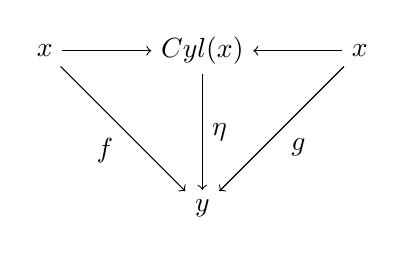
\begin{tikzpicture}
                \node (X) at (-2,0) {$x$};
                \node (X2) at (2,0) {$x$};
                \node (C) at (0,0) {$\text{Cyl}(x)$};
                \node (Y) at (0,-2) {$y$};
                \draw[->] (X) -- (C);
                \draw[->] (X2) -- (C);
                \draw[->] (C) -- node[right]{$\eta$} (Y);
                \draw[->] (X) -- node[below left]{$f$} (Y);
                \draw[->] (X2) -- node[below right]{$g$} (Y);
            \end{tikzpicture}
        \end{gather*}
        A right homotopy between $f$ and $g$ is a morphism $\lambda:x\rightarrow\text{Path}(y)$ such that the following diagram commutes:
        \begin{gather*}
            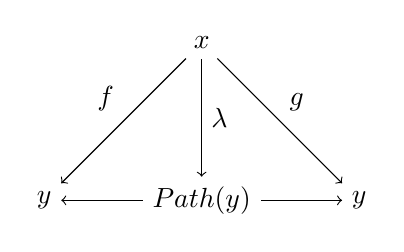
\begin{tikzpicture}
                \node (Y) at (-2,-2) {$y$};
                \node (Y2) at (2,-2) {$y$};
                \node (C) at (0,-2) {$\text{Path}(y)$};
                \node (X) at (0,0) {$x$};
                \draw[<-] (Y) -- (C);
                \draw[<-] (Y2) -- (C);
                \draw[<-] (C) -- node[right]{$\lambda$} (X);
                \draw[<-] (Y) -- node[above left]{$f$} (X);
                \draw[<-] (Y2) -- node[above right]{$g$} (X);
            \end{tikzpicture}
        \end{gather*}
    }

    \begin{property}
        If $x$ is cofibrant, every left homotopy induces a right homotopy. Dually, if $y$ is fibrant, every right homotopy induces a left homotopy.
    \end{property}
    \begin{result}
        Whenever $x$ is cofibrant and $y$ is fibrant, the relations of being left homotopic (or equivalently right homotopic) coincide on $\mathbf{M}(x, y)$ and in particular define equivalence relations. The equivalence classes are denoted by $[x, y]$.
    \end{result}
    \newdef{Homotopy equivalence}{\index{homotopy!equivalence}
        Two objects in a model category are said to be homotopy equivalent if there exists morphisms $f:x\leftrightarrows y:g$ such that $f\circ g$ and $g\circ f$ are homotopic to the identity. The morphisms $f,g$ are then said to be homotopy equivalences.
    }

    In definition \ref{cat:localization} it was shown that one can assign to every category with weak equivalences a ''homotopy category''. When the category has more structure, in this case that of a model category, one can give an equivalent definition:
    \newadef{Homotopy category}{\index{homotopy!category}
        Let $\mathbf{M}$ be a model category. The homotopy category $\mathbf{Ho}(\mathbf{M})$ is the category with the following structure:
        \begin{itemize}
            \item $\ob{Ho(M)}:=\ob{M}$, and
            \item $\text{Hom}_{\mathbf{Ho}(\mathbf{M})}(X, Y) := [X^{cf}, Y^{cf}]$.
        \end{itemize}
        In fact one often just restricts to the subcategory of $\ob{Ho(M)}$ on those objects that are fibrant and cofibrant.
    }
    \begin{property}
        The homotopy category of a model category coincides with those of the full subcategories on (co)fibrant objects:
        \begin{gather}
            \mathbf{Ho(M)}\cong\mathbf{Ho(M_f)}\cong\mathbf{Ho(M_c)}\cong\mathbf{Ho(M_{cf})}.
        \end{gather}
    \end{property}

    \begin{theorem}[Whitehead]\index{Whitehead}
        A weak equivalence between objects that are both fibrant and cofibrant is a homotopy equivalence.
    \end{theorem}

    \begin{property}
        If two model categories are Quillen equivalent, their homotopy categories are equivalent.
    \end{property}

    \begin{construct}[Hammock localization]\index{hammock localization}
        Let $\mathbf{M}$ be a model category (in fact this also works for more general categories with weak equivalences) and let $W$ be its collection of weak equivalences. First we can construct its ordinary localization $\mathbf{M}[W^-1]$. Then one can construct the so-called \textit{hammock localization} $L^H\mathbf{M}$. It can be shown that
        \begin{gather}
            \mathbf{Ho}(L^H\mathbf{M}) \cong \mathbf{M}[W^{-1}].
        \end{gather}
        This construction gives a more explicit description of the homotopy category.
    \end{construct}

    \newdef{Derived category}{\index{derived!category}
        Consider an Abelian category $\mathbf{A}$ together with its category of chain complexes $\mathbf{Ch}_\bullet(\mathbf{A})$. The derived category $\mathcal{D}(\mathbf{A})$ is defined as the localization of $\mathbf{Ch}_\bullet(\mathbf{A})$ at the collection of quasi-isomorphisms.
    }
    \remark{It can be shown in this case that one can first restrict to the naive homotopy category $\mathbf{K}(\mathbf{A})$, consisting of chain complexes and chain maps up to chain-homotopy, and then localize at the collection of quasi-isomorphisms.}

    In some cases it is useful to consider categories weaker than model categories but stronger than categories with weak equivalences. The best example is given by the full subcategories of a model category on the (co)fibrant objects. These are often easier to handle in the setting of homotopy theory. To formalize this notion we introduce the following definition:
    \newdef{Category of fibrant objects}{\index{fibrant}\index{fibration}
        A category $\mathbf{C}$ with weak equivalences $\mathbf{W}\hookrightarrow\mathbf{C}$ equipped with another subcategory $\mathbf{F}\hookrightarrow\mathbf{C}$, for which the morphisms are called \dotuline{fibrations}, such that the following conditions are satisfied:
        \begin{enumerate}
            \item $\mathbf{C}$ admits finite products.
            \item Fibrations and acyclic fibrations are preserved under arbitrary pullbacks.
            \item Every object admits a \dotuline{good path object}, i.e. a factorization of the product map $x\rightarrow x\times x$ as the composition of a weak equivalence and a fibration.
            \item All objects are \dotuline{fibrant}, i.e. the terminal map $x\rightarrow1$ is a fibration for all objects $x\in\ob{C}$.
        \end{enumerate}
    }

    We now give an important theorem in characterizing when a functor preserves weak equivalences:
    \begin{theorem}[Ken Brown's lemma]\index{Ken Brown}\label{model:ken_brown}
        Let $\mathbf{C}$ be a category of fibrant objects and let $\mathbf{D}$ be a category with weak equivalences. If a functor $\func{F}{C}{D}$ maps acyclic fibrations to weak equivalences, then it preserves all weak equivalences.
    \end{theorem}
    \remark{An analogous theorem exists for categories of cofibrant objects.}

    This lemma allows us to define \dotuline{derived functors} for functors between model categories\footnote{In fact this one is better suited for working in the $\infty$-setting.}:
    \newadef{Derived functor}{\index{derived!functor}
        Let $\func{F}{M}{N}$ be a left (resp. right) Quillen functor. The left (resp. right) derived functors are obtained by postcomposition with the cofibrant (resp. fibrant) replacement functors.
    }

\subsection{Reedy model structure}

    This section is mainly based on \cite{riehl_verity_reedy}.

    Consider a complete and cocomplete category $\mathbf{M}$ (in the remainder of this section we will often take $\mathbf{M}=\mathbf{sSet}$). For any full subcategory $\mathbf{D}\hookrightarrow\mathbf{C}$ we obtain an induced \textbf{truncation} functor\footnote{Sometimes this is called the \textbf{restriction} functor.} $\text{tr}:\mathbf{M}^\mathbf{C}\rightarrow\mathbf{M}^\mathbf{D}$. The left and right adjoints of this functor are respectively called the \textbf{skeleton} and \textbf{coskeleton} functors.
    \begin{formula}
        The adjoint functors are defined by Kan extensions and hence we can express them in terms of (co)ends and weighted (co)limits:
        \begin{gather}
            \text{sk}(X)c := \int^{d\in\ob{D}}\mathbf{C}(d, c)\cdot Xd = \colim^{\text{tr}(\mathbf{C}(-, c))}\\
            \text{cosk}(X)c := \int_{d\in\ob{D}}[\mathbf{C}(c, d), Xd] = \wlim{\text{tr}(\mathbf{C}(c, -))}X.
        \end{gather}
    \end{formula}
    \newdef{Skeletal sets}{\index{skeleton}
        Let $\mathbf{M}=\mathbf{sSet}$ and consider the inclusion $\Delta_{\leq n}\hookrightarrow\Delta$ where the former category is the full subcategory on the objects $\{[0],\ldots,[n]\}$. The $n$-truncation functor $\text{tr}_n$ discards all sets of degree higher than $n$ (or in other words it ''truncates'' a simplicial set at degree $n$).

        The $n$-skeleton functor $\text{sk}_n$ takes a simplicial set $S$ of degree $\leq n$ and freely adds degenerate simplices in degrees $>n$, i.e. it is the smallest simplicial set containing $S$ as a simplicial subset. The $n$-coskeleton functor $\text{cosk}_n$ adds a simplex in degree $>n$ whenever all of its faces are present, i.e. the $m$-simplices in $\text{cosk}_nX$ are given by the collection of all $(m+1)$-tuples of $(m-1)$-simplices that are compatible (along lower simplices).
    }
    \begin{property}[Nerves]
        The nerve functor $\func{N}{Cat}{sSet}$ from definition \ref{sheaf:nerve} is a fully faithful functor to the category of 2-coskeletal simplicial sets.
    \end{property}

    For Reedy categories \ref{cat:reedy} one can also define $n$-truncation, $n$-skeleton and $n$-coskeleton functors by restricting to the full subcategories on elements of degree $\leq n$. In this case we define the following notions:
    \newdef{Matching and latching objects}{\index{matching!object}\index{latching object}
        Let $\mathbf{R}$ be a Reedy category and consider a diagram $X\in\funccat{R}{C}$ where $\mathbf{C}$ is small. Consider the skeleton monad and coskeleton comonads (also often just called the skeleton and coskeleton functors) $\mathbf{sk}_n:=\text{sk}_n\circ\text{tr}_n$ and $\mathbf{cosk}_n:=\text{cosk}_n\circ\text{tr}_n$. The latching and matching objects of $X$ are defined as the restrictions of $\mathbf{sk}_{n-1}$ and $\mathbf{cosk}_{n-1}$ to the degree $n$ subcategory of $R$.

        The counit of the skeleton adjunction and the unit of the coskeleton adjunction give rise to the \textbf{latching} and \textbf{matching} maps.
    }
    \begin{property}
        One can also define the latching and matching objects through (co)limits. Consider the subcategory $R^+(r)$, i.e. the subcategory of $R^+/r$ on all objects except the identity $\mathbbm{1}_r$. The latching object $L_rX$ can then be shown to be isomorphic to the colimit of $X$ over $R^+(r)$.
    \end{property}

    \begin{example}[Simplicial objects]\index{Eilenberg-Zilber}
        The above property enables us to give a nice interpretation to latching objects in the case of $\mathbf{R}=\Delta^{op}$. Using the \textit{Eilenberg-Zilber} lemma one can show that the $n^{th}$ latching object of a simplicial object is given by its collection of degenerate $n$-simplices.
    \end{example}

    \newdef{Boundary}{\index{boundary}
        The boundary of a representable presheaf $\mathbf{R}(-, r)$ is defined as the latching object of the Yoneda embedding $\func{\mathcal{Y}}{R}{Psh(R)}$ at $r$. It is denoted by $\partial\mathbf{R}(-, r)$. It can be shown that $\partial\mathbf{R}(-, r)$ consists of exactly those morphisms that are not in $\mathbf{R}^-$.

        The latching map coincides with the canonical inclusion $\partial\mathbf{R}(-, r)\hookrightarrow\mathbf{R}(-, r)$.
    }
    \begin{formula}
        One can show that the latching and matching objects can be obtained through (co)limits weighted by boundaries:
        \begin{gather}
            M_rX \cong \wlim{\partial\mathbf{R}(r, -)}X\\
            L_rX \cong \colim^{\partial\mathbf{R}(-, r)}X\label{model:latching_boundary}
        \end{gather}
    \end{formula}

    From here on we will also assume $\mathbf{M}$ to be a model category (as was already the case in the previous section). We will define a model structure on the functor category $\funccat{R}{M}$ for Reedy $R$.
    \newdef{Relative matching and latching objects}{
        Consider the (weighted) colimit bifunctor $\func{\text{colim}}{Psh(R)\times[R, M]}{M}$. The \textit{Leibniz construction} (see definition \ref{model:pushout_product} below) allows us to define the relative latching object of $f:X\rightarrow Y$ at $r\in\ob{R}$ as the ''Leibniz colimit'' of the boundary inclusion $\partial\mathbf{R}(-, r)\hookrightarrow\mathbf{R}(-, r)$ and $f$.

        By equations \ref{cat:weighted_hom_colimit} and \ref{model:latching_boundary} the relative latching map is of the form $Xr\sqcup_{L_rX}L_rY\rightarrow Yr$. By suitably dualizing this construction one also gets the relative matching map $Xr\rightarrow Yr\times_{M_rY}M_rX$.
    }

    \begin{property}[Reedy model structure]
        Let $\mathbf{R}$ be a Reedy category and let $\mathbf{M}$ be a model category. The functor category $\funccat{R}{M}$ admits the following model structure:
        \begin{itemize}
            \item The weak equivalences are the levelwise weak equivalences.
            \item The (Reedy) fibrations are those morphisms for which the relative matching map is a fibration (in $\mathbf{M}$) for all $r\in\ob{R}$.
            \item The (Reedy) cofibrations are those morphisms for which the relative latching map is a cofibration (in $\mathbf{M}$) for all $r\in\ob{R}$.
        \end{itemize}
    \end{property}

\subsection{Simplicial spaces}

    A good reference for this section and in particular for the theory of Segal spaces is \cite{rezk}.

    \begin{example}[Topological spaces]
        As a first example we look at the category $\mathbf{Top}$ of topological spaces\footnote{See chapter \ref{chapter:topology} and onwards.}. This category can be endowed with the structure of a model category by taking the weak equivalences to be the weak homotopy equivalences and by taking the fibrations to be the Serre fibrations.
    \end{example}
    \begin{example}[Simplicial sets]
        As a second example we can consider the category $\mathbf{sSet}$ of simplicial sets \ref{sheaf:simplicial set}. This category can be turned into a model category by taking the weak equivalences to be the morphisms that induce weak homotopy equivalence between geometric realisations and by taking the fibrations to be Kan fibrations (fibrant objects are exactly the Kan complexes). The cofibrations are easily seen to be the levelwise injections.
    \end{example}
    \newnot{Quillen model structure}{
        The model structure defined in the above example is generally called the \textit{Quillen}-model structure on simplicial sets (since he was the first one to define it) and it is denoted by $\mathbf{sSet}_{Quillen}$.
    }
    \begin{property}\label{cat:quillen_sset_top}
        The adjoint pair of geometric realisation and singular set functors gives a Quillen equivalence between the above model categories. This result enables us to look at simplicial sets as if they were spaces and vice versa. Most of homotopy theory can be done in either categories.
    \end{property}
    \begin{property}
        Equivalent categories have weakly equivalent nerves.
    \end{property}
    The converse is not true:
    \remark{Because the information in nerves is not sufficient to distinguish between categories (and groupoids) since information about things such as invertibility is lost, i.e. weakly equivalent nerves do not necessarily come from equivalent categories, it is often useful to replace the model structure on $\mathbf{sSet}$ by an alternative one. Instead of taking the Kan complexes to be the fibrant object, \textit{Joyal} and \textit{Lurie} have shown that one can also take the (strictly weaker) quasicategories as fibrant objects to obtain a more informative structure, i.e. weak equivalences can distinguish between (nerves of) categories and groupoids. The fibrations will now be the inner Kan fibrations.}

    \newdef{Dwyer-Kan equivalence}{\index{equivalence!Dwyer-Kan}
        Consider a simplicial functor $\func{F}{C}{D}$ between two simplicial categories. This functor is called a Dwyer-Kan equivalence if
        \begin{itemize}
            \item the induced map on Hom-objects is a weak equivalence. $F$ is also said to be $\infty$-fully faithful,\footnote{This is related to the fact that simplicial categories are models for $\infty$-categories.} and
            \item the induced map on connected components $\pi_0 F:\pi_0\mathbf{C}\rightarrow\pi_0\mathbf{D}$ is an equivalence (of categories).
        \end{itemize}
    }
    \begin{property}
        Quillen equivalent model categories have Dwyer-Kan equivalent simplicial localizations.
    \end{property}

    \begin{example}[Bisimplicial sets]
        One can also look at the simplicial objects in $\mathbf{sSet}$. These are often called bisimplicial sets or \textbf{simplicial spaces}\footnote{The latter name follows from the fact that topological spaces and simplicial sets are (Quillen) equivalent.}. Since $\mathbf{sSet}$ is a model category we know from property \ref{cat:model_functor} above that $\mathbf{ssSet}$ admits itself a model structure. It can furthermore be shown that the injective model structure on $\mathbf{ssSet}$ coincides with the Reedy model structure.\footnote{This is, however, a highly nontrivial statement.}

        This allows us to define the notion of \textbf{Segal spaces}:
    \end{example}
    \newdef{Segal space}{\index{Segal!space}
        Consider a fibrant object $X$ in the injective (or Reedy) model structure on $\mathbf{ssSet}$. This bisimplicial set is called a Segal space if it satisfies the following weak form of the \textit{Segal condition}:
        \begin{gather}
            X_n\xrightarrow{\ \simeq\ }X_1\times_{X_0}\cdots\times_{X_0}X_1
        \end{gather}
        is a weak equivalence for all $n\geq1$. These maps are called \textbf{Segal maps} in general.
    }
    \newdef{Segal category}{\index{Segal!category}
        A bisimplicial set $X$ is called a Segal precategory if $X_0$ is discrete. It is called a Segal category if in addition all its Segal maps are weak equivalences.
    }

    \newdef{Mapping space}{\index{mapping space}
        Consider a Segal space $X$. For every two points $x,y\in X_0$ we define the mapping space $\text{Map}(x, y)$ as the fibre of $(d_1,d_0):X_1\rightarrow X_0\times X_0$ over the point $(x,y)$. The identity element can then be defined as $s_0x$ for all $x\in X_0$.
    }

    \newdef{Homotopy category}{\index{homotopy}
        Consider a Segal space $X$. Its homotopy category $\mathbf{Ho}(X)$ is defined as follows:
        \begin{itemize}
            \item $\text{ob}(\mathbf{Ho}(X)):=X_0$, and
            \item $\text{Hom}_{\mathbf{Ho}(X)}(x, y) := \pi_0\text{Map}(x, y)$.
        \end{itemize}
        Two points $f,g\in \text{Map}(x, y)$ are said to be \textbf{homotopic} if they are identified in $\mathbf{Ho}(X)$. A point $f\in\text{Map}(x, y)$ is called a \textbf{homotopy equivalence} if it admits both a left and a right inverse in $\mathbf{Ho}(X)$. The subspace $X_{hoequiv}\subset X_1$ consists of the components that contain homotopy equivalences.\footnote{It should be noted that if any one point in a component is a homotopy equivalence, then all points in that component are homotopy equivalences.}
    }

    \newdef{Complete Segal space}{
        A Segal space $X$ for which the map $s_0:X_0\rightarrow X_{hoequiv}$ is a weak equivalence.
    }

    \newdef{Dwyer-Kan equivalence}{\index{equivalence!Dwyer-Kan}
        A map $F$ of Segal spaces such that
        \begin{itemize}
            \item the induced map on mapping spaces is a weak equivalence, and
            \item the induced map between homotopy categories is an equivalence (of categories).
        \end{itemize}
    }
    \begin{property}
        A map of Segal spaces is a Dwyer-Kan equivalence if and only if it is a weak equivalence in the complete Segal space model structure $\mathcal{CSS}$. A map of complete Segal spaces is a Dwyer-Kan equivalence if and only if it is a levelwise weak equivalence.
    \end{property}

    Instead of changing the model structure on $\mathbf{sSet}$ to overcome the issues with taking nerves of categories or groupoids (as mentioned before) we can also change the construction of the nerve functor. Here we introduce an alternative notion introduced by \textit{Rezk}:
    \newdef{Classifying diagram}{\index{classifying!diagram}
        Consider a (small) category $\mathbf{C}$ together with the functor category $\mathbf{C}^{[n]}$ where $[n]$ is the totally ordered set on $n+1$ elements interpreted as a category. The classifying diagram of $\mathbf{C}$ is the bisimplicial set $\widetilde{N}\mathbf{C}$ defined levelwise as follows:
        \begin{gather}
            \widetilde{N}\mathbf{C}_k := N(\text{Core}(\mathbf{C}))
        \end{gather}
        where $N$ is the ordinary nerve functor and the core $\text{Core}$ was defined in \ref{cat:core}.

        The reason why this construction is better for distinguishing categories and groupoids comes from the fact that information about isomoprhisms is already captured at level 0, while information about noninvertible morphisms is only captured from level 1 onwards.
    }
    \begin{property}
        If $\mathbf{C}$ is small then $\widetilde{N}\mathbf{C}$ is a complete Segal space.
    \end{property}

    ?? COMPLETE ??

\section{Monoidal structures}

    A reference for this section is \cite{riehl_monoidal}.

    \newdef{Pushout-product}{\index{pushout}\index{Leibniz!construction}\label{model:pushout_product}
        Let $(\mathbf{M}, \otimes)$ be a closed symmetric monoidal category. Consider two morphisms $f:a\rightarrow b$ and $g:x\rightarrow y$ in $\mathbf{M}$. After taking tensor products one can form the span $a\otimes y\leftarrow a\otimes x\rightarrow b\otimes x$. If the pushout $a\otimes y\sqcup_{a\otimes x}b\otimes x$ of this diagram exists then the pushout-product $f\square g$ is the unique morphism from this pushout to $b\otimes y$ defined by the obvious diagram
        \begin{gather*}
            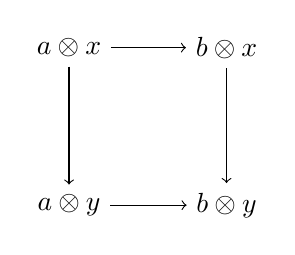
\begin{tikzpicture}
                \node (1) at (0, 0) {$a\otimes x$};
                \node (2) at (2, 0) {$b\otimes x$};
                \node (3) at (0, -2) {$a\otimes y$};
                \node (4) at (2, -2) {$b\otimes y$};
                \draw[->] (1) -- (2);
                \draw[->] (1) -- (3);
                \draw[->] (2) -- (4);
                \draw[->] (3) -- (4);
            \end{tikzpicture}
        \end{gather*}
        The dual concept is sometimes called a \textbf{pullback-hom}, \textbf{pullback-exponential} or \textbf{pullback-power} (depending on which bifunctor is used in the definition). In fact one can drop the requirement that $\mathbf{M}$ carries a monoidal structure and start from any bifunctor $\func{\circledast}{C\times D}{E}$. This more general construction is sometimes called the \textbf{Leibniz construction}.
    }

    \newdef{Monoidal model category}{\index{monoidal!model category}
        A model category $\mathbf{M}$ that carries the structure of closed symmetric monoidal category $(\mathbf{M}, \otimes, \mathbf{1})$ such that the following compatibility conditions are satisfied:
        \begin{enumerate}
            \item \textbf{Pushout-product}: The pushout-product of any two cofibrations is also a cofibration. Furthermore, if any of the two is acyclic, so is the pushout-product.
            \item \textbf{Unit}: For every cofibrant object $x$ and every cofibrant replacement $\widetilde{\mathbf{1}}$ of $\mathbf{1}$, the induced morphism $\widetilde{\mathbf{1}}\otimes x\rightarrow x$ is a weak equivalence.
        \end{enumerate}
    }
    \newdef{Quillen bifunctor}{\index{Quillen!bifunctor}
        Any bifunctor satisfying the pushout-product axiom (where in the definition of the pushout-product we replace the tensor product by the given bifunctor) such that it preserves colimits in both variables is called a \textbf{(left) Quillen bifunctor}. It should be noted that the tensor product automatically satisfies this last property in the case of closed monoidal categories.

        In fact the natural setting for defining Quillen bifunctors is that of two-variable adjunctions \ref{cat:two_variable_adjunction}. Consider such a triple of bifunctors $(\otimes, \text{hom}_L, \text{hom}_R)$.
        \begin{itemize}
            \item The bifunctor $\func{-\otimes-}{C\times D}{E}$ is said to be \textbf{left Quillen} if its pushout-product of cofibrations is again a cofibration, such that acyclicity of one of the domain morphisms leads to acyclicity of the result.
            \item The bifunctors $\text{hom}_L:\mathbf{C}^{op}\times\mathbf{E}\rightarrow\mathbf{D}$ and $\text{hom}_R:\mathbf{D}^{op}\times\mathbf{E}\rightarrow\mathbf{C}$ are said to be \textbf{right Quillen} if its ''Leibniz product'' of a cofibration and a fibration is a fibration, such that acyclicity of one of the domain morphisms leads to acyclicity of the result.
        \end{itemize}
        In fact it can be shown that one of these bifunctors being Quillen implies that the other two are also Quillen.
    }
    \remark{The fact that in the two-variable adjunction approach we do not mention preservation of (co)limits follows from the property that left (resp. right) adjoints preserve colimits (resp. limits).}


\subsection{Enrichment}

    \newdef{Enriched model category}{\index{category!enriched}\index{Joyal-Tierney calculus}
        Let $\mathcal{V}$ be a monoidal model category. A category $\mathbf{M}$ is called a $\mathcal{V}$-enriched model category if is satisfies the following conditions:
        \begin{enumerate}
            \item $\mathbf{M}$ is a $\mathcal{V}$-enriched category that is both powered and copowered over $\mathcal{V}$.
            \item The underlying category $\mathbf{M}_0$ is a model category.
            \item The copower $\cdot:\mathcal{V}\times\mathbf{M}\rightarrow\mathbf{M}$ is a left Quillen bifunctor, or equivalently, the pullback-power (with respect to the $\mathcal{V}$-powering) of any fibration and cofibration (in $\mathbf{M}_0$) is a fibration with respect to the model structure on $\mathcal{V}$ (and it is acyclic if one of the two original morphisms was).\footnote{The fact that the pullback-power axiom is satisfied if and only if the pushout-product axiom is satisfied can be proven by \textit{Joyal-Tierney calculus}.}
        \end{enumerate}
    }

    \newdef{Simplicial model category}{
        A model category enriched over the standard model category of simplicial sets $\mathbf{sSet}_{Quillen}$.
    }

\section{Cofibrant generation}
\subsection{Transfinite constructions}

    We first generalize some notions from ordinary category to the context of regular cardinals $\kappa$:
    \newdef{$\kappa$-filtered category}{\index{category!filtered}
        A  category in which every diagram with less than $\kappa$ arrows admits a cocone.
    }
    \newdef{$\kappa$-directed limit}{\index{limit!directed}
        Consider a poset $I$ such that every subposet of cardinality less than $\kappa$ has a lower bound (upper bound for directed colimits). Such a set is said to be $\kappa$-(co)directed. A limit of a diagram over this poset is called a $\kappa$-(co)directed (co)limit.
    }
    The following definition is a categorification of the previous one:
    \newdef{$\kappa$-filtered limit}{\index{limit!filtered}
        Consider a diagram $\func{D}{I}{C}$. The limit (resp. colimit) of $D$ is said to be $\kappa$-cofiltered (resp. $\kappa$-filtered) if $\mathbf{I}$ is a $\kappa$-cofiltered (resp. $\kappa$-filtered) category.
    }
    It should be noted that an analogue of property \ref{cat:directed_filtered} also holds in the $\kappa$-context, i.e. a category has all $\kappa$-directed colimits if and only if it has all $\kappa$-filtered colimits (and analogously for limits).

    \newdef{Small object}{\index{small}\index{presentable}
        An object for which there exists a regular cardinal $\kappa$ such that its covariant hom-functor preserves all $\kappa$-filtered colimits. These objects are also said to be \textbf{$\kappa$-compact} or \textbf{$\kappa$-presentable}.
    }
    \newdef{Accessible category}{\index{accessible}
        A locally small category $\mathbf{C}$ for which there exists a regular cardinal $\kappa$ such that $\mathbf{C}$ has all $\kappa$-filtered colimits and such that $\mathbf{C}$ contains a set of $\kappa$-small objects that generate all objects by $\kappa$-filtered colimits.
    }
    \newdef{Locally presentable category}{\index{presentable}
        A cocomplete accessible category.
    }

    For ordinary categories the axioms guarantee a (unique) composite of any finite number of (composable) morphisms. However, in some cases it is useful or even necessary to talk about the ''composite'' of an infinite amount of morphisms:
    \newdef{Transfinite composition}{\index{composition}\label{cat:transfinite_composition}
        Consider a category $\mathbf{C}$ with a collection of morphisms $I\subseteq\text{hom}(\mathbf{C})$. Let $\alpha$ be an infinite ordinal\footnote{See definition \ref{set:ordinal} and beyond.}. A ($\alpha$-indexed) \textbf{transfinite sequence} of morphisms in $I$ is a diagram of the form $\func{D}{\alpha}{C}$ such that:
        \begin{enumerate}
            \item Successor morphisms in $\alpha$ are mapped to elements of $I$.
            \item $D$ is \textit{continuous} in the sense that for every limit ordinal $\beta<\alpha$: $D_\beta\cong\underset{\gamma<\beta}{\text{colim}}\ D_{\gamma}$.
        \end{enumerate}
        $D_\lambda$ denotes the restriction of $D$ to the (full) subdiagram $\{\gamma:\gamma<\lambda\}$ of $\alpha$. The transfinite composition of this sequence is the induced morphism $D_0\rightarrow D\alpha\equiv\text{colim}D$.
    }
    \newdef{Cell complex}{\index{cell!complex}
        Consider a cocomplete category $\mathbf{C}$ with a designated set of morphisms $I\subseteq\text{hom}(\mathbf{C})$. A \textbf{relative} $I$-cell complex is a transfinite composition of pushouts of morphisms in $I$. An $I$-cell complex is an object such that the unique morphism from the initial object is a relative $I$-cell complex.
    }
    \newnot{Relative cell complexes}{
        The set of all relative $I$-cell complexes is often denoted by $\text{cell}(I)$.
    }

\subsection{Cofibrant generation}

    We are now ready to state a famous result by \textit{Quillen}:
    \begin{theorem}[Small object argument]\index{small object argument}
        Let $\mathbf{C}$ be a locally presentable category with a designated set of morphisms $I\subseteq\text{hom}(\mathbf{C})$. Every morphism in $\mathbf{C}$ can be factorized as the composition of a morphism in $\text{rlp}(I)$ followed by a morphism in $\text{cell}(I)$.
    \end{theorem}
    \remark{This theorem can be generalized to cocomplete categories where the morphisms in $I$ are small relative\footnote{\textit{Small relative} to a set of morphisms $I$ is defined just as ordinary smallness, but with general $\kappa$-filtered colimits replaced by those that start from morphisms in $I$.} to $\text{cell}(I)$. Sets of morphisms with this property are said to \textbf{admit a small object argument}.}

    \newdef{Cofibrantly generated model category}{\index{model!category}
        Consider a model category $\mathbf{C}$. This category is said to be cofibrantly generated by two sets of morphisms $I,J\subseteq\text{hom}(\mathbf{C})$ if it satisfies the following conditions:
        \begin{enumerate}
            \item $I$ and $J$ both admit the small object argument.
            \item The fibrations are given by $\text{rlp}(J)$.
            \item The acyclic fibrations are given by $\text{rlp}(I)$.
        \end{enumerate}
        It can be shown that the last two conditions are equivalent to the following ones:
        \begin{enumerate}
            \item[$2^*.$] The cofibrations are the retracts (in the arrow category) of $\text{cell}(I)$.
            \item[$3^*.$] The acyclic fibrations are retracts (in the arrow category) of $\text{cell}(J)$.
        \end{enumerate}
        The morphisms in $I$ and $J$ are called the \textbf{generating cofibrations} and \textbf{generating acyclic cofibrations} respectively.
    }

    Sometimes we want our model category $\mathbf{M}$ to have more weak equivalences than it already has. To this end we could try to construct a new model structure $\mathbf{M}_0$. If the cofibrations remain the same then this has some nice properties:
    \begin{itemize}
        \item The fibrations are a subclass of the original ones.
        \item The acyclic fibrations remain the same.
        \item The identity functors $\text{Id}:\mathbf{M}_0\leftrightarrows\mathbf{M}:\text{Id}$ form a Quillen adjunction.
        \item Every object in $\mathbf{M}$ is weakly equivalent (in $\mathbf{M}_0$) to one in $\mathbf{M}_0$.
    \end{itemize}
    We will now make this procedure explicit for a specific class of model categories. Let $\mathbf{M}$ be a left proper, cofibrantly generated simplicial model category and consider a class $S\subset\text{hom}(\mathbf{M})$ of cofibrations with cofibrant domain. First we introduce the notion of ''$S$-local objects'':
    \newdef{Local object}{\index{local!object}
        A fibrant object $x$ is said to be $S$-local if for all morphisms in $S$ their image under its Yoneda embedding is an acyclic Kan fibration. Analogously, a morphism is said to be an $S$-local weak equivalence if for all $S$-local fibrant objects its image under their Yoneda embeddings is an acyclic Kan fibration.
    }
    \begin{property}
        Every weak equivalence is also an $S$-local weak equivalence: $W\subset W_S$.
    \end{property}
    \begin{construct}[Left Bousfield localization]\index{Bousfield localization}
        Given a model category $\mathbf{M}$ with the same assumptions as before, we define the (left) Bousfield localization $L_S\mathbf{M}$ as the same category but with the following model structure:
        \begin{enumerate}
            \item cofibrations: $\text{cof}(L_S\mathbf{M}):=\text{cof}(\mathbf{M})$, and
            \item acyclic cofibrations: cofibrations that are also $S$-local weak equivalences.
        \end{enumerate}
    \end{construct}

    ?? FINISH ??

\section{Homotopy (co)limits}

    Consider a category $\mathbf{C}$ with weak equivalences together with diagrams $\func{F, F'}{I}{C}$. Let us assume that there exists a weak equivalence between $F$ and $F'$, i.e. a natural transformation that consists of componentwise weak equivalences. Clearly this induces a morphism between (co)limits, but it would be nice if the construction of (co)limits would also preserve the homotopy structure, i.e. we want this morphism to be a weak equivalence itself.

    The main purpose of this section is to introduce a correction of the ordinary (co)limit functors to take into account the underlying homotopical structure.

\subsection{Reedy source categories}

    We first consider the general case where we look at diagrams $\func{D}{R}{M}$ where $\mathbf{R}$ is Reedy. We first remark that the constant functor $\func{\Delta}{M}{[R, M]}$ maps weak equivalences to (pointwise) weak equivalences.\footnote{This is clearly also true even when $\mathbf{R}$ is not Reedy.} If the Reedy structure is such that the constant functor preserves cofibrations, then this functor is left Quillen and Ken Brown's lemma \ref{model:ken_brown} implies that its right Quillen adjoint, the limit functor, preserves weak equivalences. In this case we can define the \textbf{homotopy limit} $\text{holim} D$ as the functor $\lim(D\circ Q_f)$ where $Q_f$ is the fibrant replacement-functor (which in this case acts pointwise). A dual construction gives rise to \textbf{homotopy colimits}.

\subsection{Simplicially enriched diagrams}

    In the setting where we consider diagrams in categories enriched over $\mathbf{sSet}$ one can define homotopy (co)limits in a more sophisticated way. References are \cite{hocolim_riehl}. For a refresher on enriched category theory see section \ref{section:enriched_category_theory}.

    \newdef{Homotopy colimit}{
        Consider a diagram $\func{F}{I}{M}$ with $\mathbf{M}$ $\mathbf{sSet}$-enriched. The homotopy colimit of $F$ is defined as the following tensor product:
        \begin{gather}
            \text{hocolim} F := N(-/\mathbf{I})\otimes_{\mathbf{I}}F \overset{\ref{cat:copower_product}}{=} \int^{i\in\mathbf{I}}N(i/\mathbf{I})\cdot Fi.
        \end{gather}
    }
    A similar definition for homotopy limits makes use of a powering:
    \newdef{Homotopy limit}{
        Consider a diagram $\func{F}{I}{M}$ with $\mathbf{M}$ a $\mathbf{sSet}$-enriched model category. The homotopy limit of $F$ is defined as the following hom-like object:
        \begin{gather}
            \text{holim} F := \int_{i\in\mathbf{I}}[N(\mathbf{I}/i), Fi].
        \end{gather}
    }
    \begin{remark}[Bousfield-Kan map]\index{Bousfield-Kan map}
        The expressions from the above formulas are also known as the \textit{Bousfield-Kan formulas}. In fact the above definitions are not quite equivalent to the ones from the previous section. To be precise, the Bousfield-Kan formulas are strictly speaking only weakly equivalent (and hence give satisfying definitions) if we replace the objects in $\mathbf{M}$ by their (co)fibrant replacements, i.e. postcompose $F$ in the above expressions by a (co)fibrant replacement-functor.
    \end{remark}

    ?? COMPLETE ??
\chapter{Algebraic Geometry}\label{chapter:alggeom}

    References for this subject are \cite{gathmann, redbook}. For the basics on ring theory and ideals, see section \ref{section:ring}. In order to not confuse the letter $k$, often used for fields, with various indices and dimensions we will denote fields by the letter $K$.

\section{Polynomials}
\subsection{Polynomials}\index{polynomial}

    \newdef{Polynomial ring}{
        Let $R$ be a (unital commutative) ring. The polynomial ring on the indeterminates $X=\{x_i\}_{i\leq n}$ is defined as the free commutative $R$-algebra on $X$. It will be denoted by $R[X]\equiv R[x_1,\ldots,x_n]$.
    }

    \newdef{Degree}{\index{degree}
        \nomenclature[O_deg]{$\deg(f)$}{Degree of the polynomial $f$.}
        The degree of a polynomial $f$ is equal to the largest integer $d$ such that $f$ contains a monomial $x_1^{i_1}\cdots x_n^{i_n}$ for which $i_1+\cdots+i_n=d$. It is often denoted by $\deg(f)$.
    }
    \newdef{Monic polynomial}{A polynomial for which the highest degree term has coefficient $1$.}

    \begin{theorem}[Fundamental theorem of algebra]\index{fundamental theorem!of algebra}\label{linalgebra:fundamental_theorem_of_algebra}
        Consider a polynomial $f\in\mathbb{C}[x]$ with $\deg(f)\geq 1$. Then $f$ has at least 1 root in $\mathbb{C}$.
    \end{theorem}
    \begin{result}
        If $f\in \mathbb{C}[x]$ is a monic polynomial with $\deg(f)\geq1$, we can write:
        \begin{gather*}
            f(x) = \prod_{i=1}^k(x-a_i)^{n_i}
        \end{gather*}
        where $a_1,\ldots, a_k\in\mathbb{C}$ and $n_1,\ldots, n_k\in\mathbb{N}$.
    \end{result}

    \newdef{Transcendental element}{\index{transcendental}\index{algebraic}
        Consider a field $K$ and a field extension $L/K$. An element $x\in L$ for which there exist no nontrivial polynomials $p$ over $K$ such that $p(x) = 0$, is said to be transcendental, otherwise it is said to be \textbf{algebraic}.
    }

    \newdef{Algebraic dependence}{
        Consider a commutative ring $R$ and a subring $S\subset R$. An element $r\in R$ is said to be algebraically dependent on $S$ if it is the root of a polynomial in $S[x]$.
    }
    As a subcase of the above we have:
    \newdef{Integral dependence}{
        Consider a commutative ring $R$ and a subring $S$. An element $r\in R$ is said to be integrally dependent on $S$ if it is the root of a monic polynomial in $S[x]$.
    }
    \remark{Since every nonzero element in a field is invertible, one can always turn a general polynomial into a monic polynomial. Hence over a field the concepts of algebraic and integral dependence coincide.}

\subsection{Roots}

    \begin{formula}[Vieta]\index{Vieta}
        Consider a polynomial of order $n$. By the fundamental theorem of algebra this polynomial has $n$ complex roots. Vieta's formulas relate the coefficients of the polynomial to its roots:
        \begin{gather}
            \sum_{1\leq I_1\leq\ldots\leq i_k\leq n}\left(\prod_{j=1}^kr_{i_j}\right) = (-1)^k\frac{a_{n-k}}{a_n}
        \end{gather}
        where $k\leq n$. For $k=1$ and $k=n$ this gives the well-known sum and product formulas:
        \begin{align}
            r_1+r_2+\cdots+r_n &= -\frac{a_{n-1}}{a_n}\\
            r_1r_2\cdots r_n &= (-1)^n\frac{a_0}{a_n}.
        \end{align}
    \end{formula}
    \begin{example}
        For quadratic polynomials $ax^2+bx+c$ one recovers the following well-known formulas:
        \begin{align}
            r_1+r_2 &= -\frac{b}{a}\\
            r_1r_2 &= \frac{c}{a}.
        \end{align}
    \end{example}

\subsection{Ideals}

    \begin{theorem}[Weak Nullstellensatz]\index{Nullstellensatz}
        Consider an algebraically closed field $K$ and form the polynomial ring $R=K[x_1, \ldots, x_n]$. An ideal $I\subset R$ is maximal if and only if it is of the form \[(x_1-a_1, \ldots, x_n-a_n)\] with $a_i\in K$ for all $i\leq n$.
    \end{theorem}
    \begin{result}
        There exists a bijection between $K^n$ and the set of maximal ideals of $K[x_1, \ldots, x_n]$.
    \end{result}
    \begin{result}
        Consider a collection of polynomials $\{f_i\}_{i\in I}\subset K[x_1, \ldots, x_n]$. If these polynomials do not have a common zero, then the ideal they generate is the unit ideal.
    \end{result}

\section{Varieties}\label{section:varieties}

    From here on we assume $K$ to be an algebraically closed field. For notational simplicity and to differentiate between $K^n$ as a vector space and as a set (or variety further down) we first introduce the notion of affine space:
    \newdef{Affine space}{\index{affine!space}
        By $\mathbb{A}^n$ we denote the underlying set of the vector space $K^n$:
        \begin{gather}
            \mathbb{A}^n := \{(a_1,\ldots,a_n)\in K^n\}.
        \end{gather}
    }

    \newdef{Algebraic set}{\index{algebraic!set}\index{irreducible!algebraic set}\index{variety}\label{alggeom:variety}
        Consider a finite set of polynomials in $K[x_1, \ldots, x_n]$. It is not hard to show that the zero locus of these polynomials depends only on the ideal spanned by them and hence we define the algebraic set associated to an ideal $I\subset K[x_1, \ldots, x_N]$ to be
        \begin{gather}
            V(I) := \big\{(a_1,\ldots,a_n)\in\mathbb{A}^n: f(a_1,\ldots,a_k)=0\ \ \forall f\in I\big\}.
        \end{gather}
        A set $S\in\mathbb{A}^n$ is said to be an \textbf{(affine) algebraic set} if there exists an ideal $I$ such that $S=V(I)$. An algebraic set $S\in\mathbb{A}^n$ is said to be \textbf{irreducible} if it is not the union of two strictly smaller algebraic sets. Irreducible algebraic sets are also called \textbf{affine varieties}.
    }
    \sremark{Some authors (such as in \cite{gathmann}) make no distrinction between general algebraic sets and affine varieties.}

    \begin{property}\index{Hilbert!basis theorem}
        By \textit{Hilbert's basis theorem} one can obtain any algebraic set as the zero locus of a finite number of polynomials.
    \end{property}

    Given an algebraic set $S$, one defines the set $I(S)$ as the ideal of polynomials which vanish on $S$. The following theorem gives an important relation between algebraic sets and ideals.
    \begin{theorem}[Hilbert's Nullstellensatz]\index{Hilbert!Nullstellensatz}\index{Nullstellensatz|seealso{Hilbert}}
        Let $J$ be an ideal in $K[x_1,\ldots,x_n]$ and let $\sqrt{J}$ denote its radical. The following relation holds for all $J$:
        \begin{gather}
            I(V(J)) = \sqrt{J}.
        \end{gather}
    \end{theorem}
    Similar to the case of the weak Nullstellensatz we obtain the following result
    \begin{result}
        There exists a bijection between the algebraic subsets of $\mathbb{A}^n$ and the radical ideals in $K[x_1, \ldots, x_n]$. The irreducible algebraic sets correspond to the prime ideals (by the \textit{Noetherian decomposition theorem}).
    \end{result}

    \newdef{Morphism of varieties}{\index{morphism!of varieties}
        Let $V_1\subset\mathbb{A}^{n_1}, V_2\subset\mathbb{A}^{n_2}$ be two algebraic sets. A morphism $\varphi:V_1\rightarrow V_2$ is a function that can be expressed in the following way:
        \begin{gather}
            \varphi(x_1,\ldots,x_{n_1}) = \big(f_1(x_1,\ldots,x_{n_1}), \ldots, f_{n_2}(x_1,\ldots,x_{n_1})\big)
        \end{gather}
        where $f_i\in K[x_1,\ldots,x_{n_1}]$ for all $i\leq n_2$.
    }
    A closely related notion is that of rational maps:
    \newdef{Rational map}{\index{rational!map}\index{dominant}\index{birational|see{rational}}
        Consider two affine varieties $X, Y$. A rational map $f:X\rightarrow Y$ is an equivalence class of pairs $(U, f_U)$, where $U$ is a nonempty open subset and where $f_U:U\rightarrow Y$, under the following relation: $(U, f_U)\sim(V, f_V)$ if and only if $f_U=f_V$ on a nonempty subset of $U\cap V$.

        A rational map is said to be \textbf{dominant} if for one of its representatives $(U, f)$ the image $f(U)$ is dense. Dominance of rational maps assures that their composition exists and is well-defined.

        A rational map $f:X\rightarrow Y$ is said to be \textbf{birational} if it is dominant and if there exists a rational map $g:Y\rightarrow X$ such that $f\circ g = \text{id}_Y$ and $g\circ f = \text{id}_X$.
    }

    \newdef{Coordinate ring}{\index{coordinate!ring}\index{function!field}\index{rational!function}
        Consider the polynomial ring $K[x_1,\ldots,x_n]$ and let $V$ be an algebraic set in $\mathbb{A}^n$. The coordinate ring of $V$ is defined as the following quotient:
        \begin{gather}
            \Gamma(V) := K[x_1,\ldots,x_n]/I(V).
        \end{gather}
        The elements of this ring are the $K$-valued polynomials in the coordinates on $V$.

        If $V$ is irreducible it follows from the Nullstellensatz that $I(V)$ is a prime ideal and hence that $\Gamma(V)$ is an integral domain. This property allows us to construct the field of fractions $K(V)$. This field is called the \textbf{function field} of $V$ and the elements of $K(V)$ are called \textbf{rational functions} on $V$. It can be shown that the rational functions are exactly the rational maps $V\rightarrow\mathbb{A}^1$.
    }

    It should be noted that every morphism of varieties induces an $K$-morphism on the associated affine ring by precomposition. This gives rise to the following property:
    \begin{property}[Affine varieties and finitely generated algebras]\label{alggeom:variety_domain_equivalence}
        $\Gamma$ gives an equivalence between the category of algebraic sets and the category of finitely-generated reduced $K$-algebras. This equivalences passes to an equivalence between the subcategories on affine varieties and integral domains.
    \end{property}

    \newdef{Dimension}{\index{dimension}
        The dimension of an affine variety $V$ is given by the \textit{(Krull) dimension} of its coordinate ring.
    }

\subsection{Topology}

    A topology on varieties can be constructed in the following way:
    \newdef{Zariski topology}{\index{Zariski!topology}
        A set in $\mathbb{A}^n$ is closed exactly if it is an algebraic set. A basis for this topology is given by the zero loci $B_f = \{x\in\mathbb{A}^n: f(x)\neq 0\}$ for $f\in K[x_1,\ldots,x_n]$. This topology turns an affine variety into an irreducible space.

        On an algebraic subset $V\subset\mathbb{A}^n$ one defines the Zariski topology as the induced topology of the one on $\mathbb{A}^n$. A basis for this induced Zariski topology is given by the sets $B_f$ as above but where $f$ is now an element in $\Gamma(V)$.
    }

    \begin{property}[Density]
        Any open subset of an affine variety is dense.
    \end{property}

    By dualizing our point of view we can instead focus on the coordinate rings and construct varieties as a derived notion. To this intent we define the structure sheaf\footnote{From here on the content of chapter \ref{chapter:sheaf} on sheaf theory will be a prerequisite.} of a variety:
    \newdef{Structure sheaf}{\index{structure!sheaf}\index{regular!function}\label{alggeom:structure_sheaf}
        Consider an affine variety $X$ and its associated coordinate ring $R$. Now for any point $x\in X$ one can consider the set of functions $m_x\subset R$ which vanish on $x$. This is a prime ideal so one can construct the localization of $R$ at $m_x$:
        \begin{gather}
            \mathcal{O}_x := R_{m_x} = \{f/g : f,g\in R\text{ and }g(x)\neq0\}.
        \end{gather}
        For every open subset $U\subset X$ we can then define the ring of functions on $U$ as follows:
        \begin{gather}
            \mathcal{O}_X(U) := \bigcap_{x\in U}\mathcal{O}_x.
        \end{gather}
        This way $\mathcal{O}_X$ defines a sheaf with stalks given by $\mathcal{O}_x$. By property \ref{algebra:localization_local_ring} all stalks $\mathcal{O}_x$ are local rings and hence $(X,\mathcal{O}_X)$ is a locally ringed space. The residue field of these local rings is equal to the base field $K$.

        The elements of $\mathcal{O}_X(U)$ are called the \textbf{regular functions} on $U$. To make the above construction more explicit: A map $\varphi:X\rightarrow K$ is said to be regular at a point $x\in X$ if there exists an open neihgbourhood $U\ni x$ and polynomials $f,g\in R$ with $g\neq0$ and $\varphi=f/g$ on $U$. As for continuous functions, we say the map $\varphi$ is regular on $X$ if it is regular at every point $x\in X$.
    }

    \begin{property}
        Let $f\in R=\Gamma(X)$ be a function on $X$ and consider the set $B_f$, i.e. the complement of the zero locus of $f$. Then we have $\mathcal{O}_X(B_f) = R_f$ (where $R_f$ denotes the localization of $R$ at $f$ conform \ref{algebra:localization_notation}). In particular we find for the global sections functor that
        \begin{gather}
            \Gamma(X,\mathcal{O}_X) = R.
        \end{gather}
        This property explains the notation $\Gamma(X)$ introduced before.
    \end{property}
    \remark{Both the rings $\mathcal{O}_X(U)$ and $\mathcal{O}_x$ are subrings of the function field $K(X)$.}

    \newadef{Affine variety}{\index{variety!affine}
        Any topological space $X$ equipped with a sheaf $\mathcal{F}$ of $K$-valued functions such that $X$ is isomorphic to an irreducible algebraic set $\Sigma$ and such that $\mathcal{F}$ is isomorphic to the structure sheaf $\mathcal{O}_\Sigma$ is called an affine variety. An open subset of an affine variety is called a \textbf{quasi-affine variety}.
    }
    Using the notion of a regular function we can restate the definition of a morphism of affine varieties:
    \newadef{Morphism}{\index{morphism!of varieties}
        A continuous function between affine varieties $f:X\rightarrow Y$ such that precomposition by $f$ preserves regular functions.
    }

    \begin{property}[Identity theorem]
        If two regular maps coincide on a nonempty open subset then they are equal.
    \end{property}

    \newdef{Generic stalk}{\index{stalk!generic}
        For the construction of the stalk of the structure sheaf over a point $x$ one takes a direct limit over all open sets containing $x$. This way we obtained the local ring $\Gamma(X)_{m_x}$ which was a subring of the field of fractions $K(X)$ of $\Gamma(X)$. Now, using a similar definition one can recover all of $K(X)$.

        Instead of taking a direct limit over the open sets containing a certain point $x\in X$, we take a direct limit over all open sets in $X$:
        \begin{gather}
            \mathcal{O}_{\tilde{x}} := \varinjlim_{U\subset\Sigma}\mathcal{O}_\Sigma(U).
        \end{gather}
        This stalk is called the generic stalk of $X$ and it is isomorphic to $K(X)$.
    }

\subsection{Varieties}

    In this section we move from the global to the local picture. A first step is the definition of a prevariety:
    \newdef{Prevariety}{\index{prevariety}
        Let $X$ be a topological space equipped with a sheaf $\mathcal{O}_X$ of $K$-valued functions. The space $X$ is said to be a prevariety if $X$ is connected and if there exists a finite covering $\{U_i\}_{i\in I}$ of $X$ such that every couple $(U_i, \mathcal{O}_X|_{U_i})$ forms an affine variety.
    }
    \newdef{Morphism}{\index{morphism!of prevarieties}
        Consider two prevarieties $(X, \mathcal{O}_X)$ and $(Y, \mathcal{O}_Y)$. A morphism between them is a continuous function $f:X\rightarrow Y$ such that
        \begin{gather}
            g\in\Gamma(V, \mathcal{O}_Y) \implies gf\in\Gamma(f^{-1}V, \mathcal{O}_X)
        \end{gather}
        for all open sets $V\subset Y$, i.e. morphism of prevarieties are just morphisms of ringed spaces.
    }

    \remark{It can be shown that every prevariety $X$ is irreducible and hence the open sets form a direct system. This way we can, as in the case of affine varieties, define the \textbf{generic stalk} of an arbitrary sheaf $\mathcal{F}$. For the structure sheaf $\mathcal{O}_X$ this generic stalk is called the \textbf{function field} $K(X)$. It coincides with the function field of every open affine subset of $X$.

    \begin{construct}[Gluing]\label{alggeom:gluing}
        Consider two prevarieties $X, Y$ together with an isomorphism $f:U\cong W$ between open subsets $U\subset X, V\subset Y$. The prevarieties can be glued together along $f$ as follows: One first builds the attaching space\footnote{See definition \ref{topology:attaching_space}.} $U\sqcup_fY$ with its canonical topology and then define the regular functions on a subset to be those that come from regular functions on (subsets of) $X$ and $Y$.
    \end{construct}

    \newdef{Variety\footnotemark}{\index{variety}\label{alggeom:abstract_variety}
        \footnotetext{Sometimes also called a \textbf{separated prevariety}.}
        A prevariety $X$ for which the diagonal $\Delta_X$ is closed in $X\times X$. It should be noted that every affine variety is a variety, but not the other way around.
    }
    \remark{The motivation for this definition is property \ref{topology:hausdorff}. In general topology it is well-known that a lot of pathological spaces can be excluded by restricting to Hausdorff spaces, i.e. spaces where distinct points admit disjoint neighbourhoods. Because open subsets of irreducible spaces have nonempty intersections this property is sadly enough not very useful in the study of varieties. However, the equivalent definition using closedness of the diagonal remains useful if we do not consider the product topology on $X\times X$ but instead use the ''gluing''-topology from construction \ref{alggeom:gluing} above.

    The following two closure properties are very important:
    \begin{property}\label{alggeom:closed_graph}
        Consider a prevariety morphism $f:X\rightarrow Y$ where $Y$ is a variety. The graph of $f$ is closed in $X\times Y$.
    \end{property}
    \begin{property}
        Consider two prevariety morphisms $f,g:X\rightarrow Y$ where $Y$ is a variety. The set on which $f$ and $g$ coincide is closed in $X$.
    \end{property}

\subsection{Projective varieties}

    \newdef{Projective space}{\index{projective!space}
        Consider the vector space $K^n$ (over $K$ istelf). The projective space $\mathbb{P}_{n-1}(K)$ or $K\mathbb{P}^{n-1}$ is defined as the quotient space of $K^n$ under the following equivalence relation:
        \begin{gather}
            (x_1,\ldots,x_n)\sim(y_1,\ldots,y_n)\iff\exists\lambda\in K^\times:\forall i\leq n:x_i=\lambda y_i.
        \end{gather}
        The equivalence class of a vector $(x_1,\ldots,x_n)$ will be denoted by $[x_1:\cdots:x_n]$.
    }

    Consider the subset \[K_{\text{hom}}[x_0,\ldots,x_n]\subset K[x_0,\ldots,x_n]\] consisting of all homogeneous polynomials, i.e. all $f\in K[x_0,\ldots,x_n]$ such that $f(\lambda x_0,\ldots,\lambda x_n)=\lambda^df(x_0,\ldots,x_n)$ for some $d\in\mathbb{N}$. This implies that $f(\lambda x_0,\ldots,\lambda x_n) = 0 \iff f(x_0,\ldots,x_n) = 0$ and hence zero loci of homogeneous polynomials are well-defined subsets of the projective space $\mathbb{P}_n(K)$.
    \newdef{Projective algebraic set}{\index{algebraic!set}\index{Zariski!topology}
        So as in the case of affine algebraic sets we can define two operations: Let $I$ be a homogeneous ideal, i.e. an ideal in $K[x_0,\ldots,x_n]$ that is generated by homogeneous polynomials. We define the projective algebraic set $V_p(I)$ as the zero locus of $I$:
        \begin{gather}
            V_p(I) := \{x\in\mathbb{P}_n(K):f(x)=0\ \forall f\in I\}.
        \end{gather}
        Given a projective algebraic set $X\in\mathbb{P}_n(K)$ one can define the ideal $I_p(X)$ as follows:
        \begin{gather}
            I_P(X) := (f\in K_{\text{hom}}[x_0,\ldots,x_n]\mid f(x)=0\ \forall x\in X)
        \end{gather}
        i.e. the ideal $I_p(X)$ is generated by all homogeneous polynomials vanishing on $X$. The Zariski topology on $\mathbb{P}_n(K)$ is defined such that the clsoed sets are exactly the projective algebraic sets.
    }

    \begin{theorem}[Projective Nullstellensatz]\index{Nullstellensatz}
        For all homogeneous ideals $I$, except $I_0=(x_1,\ldots,x_n)$, one finds that
        \begin{gather}
            I_p(V_p(I)) = \sqrt{I}.
        \end{gather}
    \end{theorem}
    \begin{result}
        As before this implies that there exists a bijection between the projective algebraic sets in $\mathbb{P}_n(K)$ and the homogeneous radical ideals (except for $I_0$) in $K[x_0,\ldots,x_n]$.
    \end{result}

    \newdef{Coordinate ring}{\index{coordinate!ring}
        As for affine algebraic sets we define the coordinate ring of a projective algebraic set $X$ as the following quotient:
        \begin{gather}
            \Gamma(X) := K[x_0,\ldots,x_n]/I_p(X).
        \end{gather}
    }

    The construction for regular functions on affine varieties (see definition \ref{alggeom:structure_sheaf}) cannot be extended to projective spaces in a straightforward way. Consider for example a polynomial $f\in K[x_0,\ldots,x_n]$. This polynomial does not form a well-defined function on a projective algebraic set $V_p(I)\subset \mathbb{P}_n(K)$ even if $f$ is homogeneous, since changing the homogeneous coordinates on $V_p(I)$ changes the value of $f$ (only the zero locus is invariant). However, the ratio of two homogeneous polynomials of the same degree does form a well-defined function on $V_p(I)$.

    Since the ideal $I$ is homogeneous, the quotient $R=K[x_0,\ldots,x_n]/I$ is a graded algebra. Let us denote by $K(X)$ the zeroth order part of the localization of $R$ by the homogeneous elements:
    \begin{gather}
        K(X) := \{f/g\mid f,g\in R_n\text{ for some }n\in\mathbb{N}\}.
    \end{gather}
    Now, although an element $f\in R_n$ does not give a well-defined function on $X$, the property $f(x)\neq0$ is clearly preserved under scale transformations. Hence we can define a ring $\mathcal{O}_x$ as before:
    \begin{gather}
        \mathcal{O}_x := \{f/g\in K(X): g(x)\neq 0\}.
    \end{gather}
    This ring has a maximal ideal $I_x = \{f/g\in K(X):f(x)=0, g(x)\neq 0\}$ such that all elements in $\mathcal{O}_x$ are invertible and so by property \ref{algebra:local_ring_invertible} $\mathcal{O}_x$ is a local ring. We can then construct a sheaf $\mathcal{O}_X$ using the same procedure as for affine varieties to turn our projective space into a locally ringed space:
    \begin{gather}
        \mathcal{O}_X(U) = \bigcap_{x\in U}\mathcal{O}_x.
    \end{gather}

    \begin{property}[Variety]
        For every projective variety $X\subset\mathbb{P}_n(K)$ the pair $(X, \mathcal{O}_X)$ is locally isomorphic to an affine variety and as such every projective variety is in particular a variety in the sense of definition \ref{alggeom:abstract_variety}.
    \end{property}
    \begin{property}[$\mathbb{A}^n$ in $\mathbb{P}_n(K)$]
        Consider the affine variety $\mathbb{A}^n$. This set admits a bijective mapping onto an open subset of $\mathbb{P}_n(K)$ as follows:
        \begin{gather}
            \varphi:\mathbb{A}^n\rightarrow U_0:(x_1,\ldots,x_,n)\mapsto[1:x_1:\cdots:x_n].
        \end{gather}
        It can be shown that this map is a homeomorphism if we equip both spaces with the Zariski topology.
    \end{property}

    \begin{property}[Schubert decomposition]\index{Schubert!decomposition}\index{Schubert!cell}\index{Bruhat cell}
        The projective space $\mathbb{P}_n(K)$ admits a decomposition of the form
        \begin{gather}
            \mathbb{P}_n(K) = \bigcup_{i=0}^n K^i
        \end{gather}
        where the union should be interpreted on the level of the underlying sets. In fact one can refine this to a statement in topology. The projective space $\mathbb{P}_n(K)$ admits the structure of a CW-complex where with one $k$-cell in every dimension (namely $\mathbb{A}^k$). These cells are also called \textbf{Bruhat cells} \textbf{Schubert cells}. (The precise distinction won't be of any relevance to us.)
    \end{property}

    \begin{example}[Finite fields]\index{Fano plane}
        Consider a finite field $\mathbb{F}_q$. Using the above decomposition we can easily compute the cardinality of $\mathbb{P}_n(\mathbb{F}_q)$:
        \begin{gather*}
            |\mathbb{P}_n(\mathbb{F}_q)| = \sum_{i=0}^n|\mathbb{F}_q^i| = \sum_{i=0}^nq^i = [n+1]_q.
        \end{gather*}
        For example, the \textbf{Fano plane} $\mathbb{F}_2\mathbb{P}^2$ has cardinality 7.
    \end{example}

    \begin{construct}[Blow-up]
        Consider an algebraic set $X\subseteq\mathbb{A}^n$ together with a set of regular functions $\{f_1,\ldots,f_k\}\subset\Gamma(X)$. Now define the subvariety $Y$ by $X\backslash V(f_1,\ldots,f_k)$. By definition these functions do not all vanish simultaneously on $Y$ and hence we have a well-defined map \[f:Y\rightarrow \mathbb{P}_n(K):x\mapsto\Big(f_1(x),\ldots,f_k(x)\Big).\] The graph of this morphism is closed in $Y\times\mathbb{P}_{n-1}(K)$ by property \ref{alggeom:closed_graph}, but not in $X\times\mathbb{P}_{n-1}(K)$. Its closure in the latter space is called the blow-up $\widetilde{X}$ of $X$ at $f_1,\ldots,f_k$. The obvious projection map $\pi:\widetilde{X}\rightarrow X$ is sometimes also called the blow-up (map). The graph $\Gamma_f$ is clearly isomorphic to $Y$ and its complement $\pi^{-1}(V(f_1,\ldots,f_k))$ in $\widetilde{X}$ is called the \textbf{exceptional set} (of the blow-up).

        If $X$ is irreducible, then there exists a birational morphism $X\rightarrow\widetilde{X}$.
    \end{construct}

    \begin{property}[Explicit description]
        Consider an algebraic set $X\subseteq\mathbb{A}^n$ together with its blow-up $\widetilde{X}$ at $\{f_1,\ldots,f_k\}$. One can prove that the following inclusion holds:
        \begin{gather}
            \widetilde{X}\subseteq\{(x,y)\in X\times\mathbb{P}_{n-1}(K):y_if_j(x)=y_jf_i(x)\ \forall i,j\leq n\}.
        \end{gather}
        In the case of $X=\mathbb{A}^n$ and $f_i(x):=x_i$ one can even prove that this inclusion is an equality. Since the zero locus of the coordinate functions is $\{0\}$ we find that the exceptional set of this blow-up is exactly $\mathbb{P}_{n-1}(K)$.
    \end{property}

\section{\difficult{Schemes}}\label{section:schemes}
\subsection{Spectrum of a ring}

    \newdef{Spectrum}{\index{spectrum}\index{Zariski!topology}
        \nomenclature[S_Spec]{Spec$(R)$}{Spectrum of a commutative ring $R$.}
        Let $R$ be a commutative ring. The spectrum $\text{Spec}(R)$ is defined as the set of prime ideals of $R$. This set can be turned into a topological space by equipping it with the \textbf{Zariski topology}: Let $V_I$ be the set of prime ideals containing the ideal $I$. The collection of closed sets, inducing the Zariski topology, is given by $\{V_I\}_{I\text{ ideal of }R}$.
    }
    \remark{A basis for the above topology is given by the sets $D_f = \{I_p\not\ni f:f\in R, I_p \text{ is a prime ideal}\}$.}

    \begin{property}
        Spec$(R)$ is a compact $T_0$ space.
    \end{property}

    \newdef{Structure sheaf}{\index{structure!sheaf}
        Given a spectrum $X=$ Spec$(R)$, equipped with its Zariski topology, we can define a sheaf\footnote{In fact this is merely a \textit{B-sheaf} as it is only defined on the basis of the topology. However, every B-sheaf can be extended to a sheaf by taking the appropriate limits.} $\mathcal{O}_X$ by setting $\forall f\in R: \Gamma(D_f, \mathcal{O}_X) = R_f^*$, where $R_f^*$ is the localization of $R$ with respect to the monoid of powers of $f$.
    }

    \begin{property}
        The spectrum Spec$(R)$ together with its structure sheaf forms a ringed space.
    \end{property}

\subsection{Affine schemes}

    \newdef{Affine scheme}{\index{scheme}
        A locally ringed space, isomorphic to the spectrum $\text{Spec}(R)$ for some commutative ring $R$, is called an affine scheme.
    }

    \begin{property}
        There exists an equivalence of categories $\mathbf{AffSch}\cong\mathbf{CRing}^{op}$.
    \end{property}

\subsection{Zariski tangent space}

    \newdef{Tangent cone}{\index{tangent!cone}\index{initial!part}
        Consider an affine variety $X=V(I)$. The tangent cone to $X$ at the origin is defined as the zero locus of the ''initial ideal'' of $I$:
        \begin{gather}
            C_0X := V(\{f^{in}:f\in I\})
        \end{gather}
        where $f^{in}$ denotes the \textbf{initial part} of $f$, i.e. the sum of the smallest degree monomials in $f$.
    }

    \newdef{Tangent space}{\index{tangent!space}
        Consider a variety $X$ and choose any point $x\in X$. By choosing a suitable affine chart we can assume that $x=0$. This implies that any polynomial $f\in I(X)$ has a vanishing constant term. The tangent space at $x$ is defined as follows:
        \begin{gather}
            T_xX := V(\{f^{[1]}:f\in I(X)\})
        \end{gather}
        where $f^{[1]}$ denotes the linear part of a polynomial $f$.
    }
    \begin{property}
        For $x=0$ we obtain that $I(x) = (x_1,\ldots,x_n)/I(X)$. Then there exists a natural isomorphism
        \begin{gather}
            I(x)/I(x)^2\cong\hom_K(T_xX, K).
        \end{gather}
        The tangent space at $X$ is thus the dual of $I(a)/I(a)^2$.
    \end{property}

    It is not so hard to prove that this property can in fact easily be transported to arbitrary points $x'\in X$ if we replace the ideal $I(x)$ by the maximal ideal $\mathcal{O}_{x'}$ of the structure sheaf $\mathcal{O}_X$ at $x'$. Therefore we can give the following general definition:
    \begin{definition}[Zariski tangent space]\index{Zariski!tangent space}\index{tangent!space|seealso{Zariski}}
        Consider a variety $X$ with structure sheaf $\mathcal{O}_X$. At every point $x\in X$ the ring $\mathcal{O}_{X, x}$ is a local ring and hence we obtain a maximal ideal $\mathfrak{m}_x$. The quotient $\mathfrak{m}_x/\mathfrak{m}_x^2$ is a vector space over the residue field $\mathcal{O}_{X, x}/\mathfrak{m}_x$. It is called the Zariski cotangent space at $x\in X$. Its algebraic dual is called the Zariski tangent space at $x\in X$.
    \end{definition}

\section{Algebraic groups}

    \newdef{Linear algebraic group}{
        A subgroup of $\text{GL}(n, F)$ defined by a (finite) set of polynomials in the matrix coefficients.
    }
    \begin{property}
        From the definition it is immediately clear that intersections of algebraic groups are again algebraic.
    \end{property}

    ?? COMPLETE ??
\chapter{Topos theory}

\section{Elementary topoi}

    \newdef{Subobject classifier}{\index{subobject!classifier}
        Consider a finitely complete category (in fact the existence of a terminal object suffices). A subobject classifier is a mono\footnote{The symbol for this morphism will become clear in subsection \ref{cat:internal_logic}.} $\texttt{true}:\mathbf{1}\hookrightarrow\Omega$ from the terminal object such that for every mono $\phi:a\hookrightarrow b$ there exists a unique morphism $\chi:b\rightarrow\Omega$ such that the following pullback square exists:
        \begin{figure}[ht!]
            \centering
            \begin{tikzcd}[ampersand replacement=\&, row sep=4em,column sep=4em, minimum width=2em]
                a \arrow[r, "!"] \arrow[d, hook, "\phi"'] \& \mathbf{1} \arrow[d, hook, "\texttt{true}"]\\
                b \arrow[r, "\chi!"] \& \Omega
            \end{tikzcd}
            \caption{Subobject classifier.}
            \label{fig:subobject_classifier}
        \end{figure}
    }
    \begin{adefinition}
        Consider a well-powered category $\mathbf{C}$. The assignment of subobjects Sub$(a)$ to an object $a\in\ob{C}$ is a contravariant functor $\mathcal{S}:\mathbf{C}\rightarrow\mathbf{Set}$. A subobject classifier $\Omega$ is a representation of this functor, i.e. the following isomorphism is natural in $a$:
        \begin{gather}
            \mathcal{S}(a)\cong\text{hom}_{\mathbf{C}}(a, \Omega).
        \end{gather}
    \end{adefinition}

    \begin{example}
        The category $\mathbf{Set}$ has a subobject classifier, namely the 2-element set.
    \end{example}

    \newdef{Elementary topos}{\index{topos!elementary}
        An elementary topos is a Cartesian closed category containing a subobject classifier. Equivalently, one can define an elementary topos as a finitely complete category in which all power objects exist.

        The power object $Pa$ of $a$ is related to the subobject classifier $\Omega$ through the exponential by the following relation:
        \begin{gather}
            Pa = \Omega^a.
        \end{gather}
    }

    \begin{example}[Slice category]
        Let $\mathcal{C}$ be a topos. For every object $c\in\ob{C}$ the slice category $\mathbf{C}/c$ is also a topos. The subobject classifier is given by $\pi_2:\Omega\times c\rightarrow c$.
    \end{example}

    \begin{property}[Balanced]
        All monos in a topos are regular. Hence every mono arises as an equalizer and every epic equalizer is necessarily an isomorphism. It follows that every topos is balanced\footnote{See definition \ref{category:balanced}.}.
    \end{property}

    \begin{property}[Epi-mono factorization]\index{image}
        Every morphism $f:a\rightarrow b$ in a topos factorizes uniquely as an epi followed by a mono:
        \begin{gather}
            a\overset{e}{\twoheadrightarrow} c\overset{m}{\rightarrowtail} b.
        \end{gather}
        The mono is called the \textbf{image} of $f$.
    \end{property}

\subsection{Topological sheafs}

    \begin{property}[Presheaf topos]\label{topoi:sheaf_topos}
        Consider the presheaf category\footnote{See chapter \ref{chapter:sheaf} for the application of sheafs in topology.} $\mathbf{Psh}(X) = \widehat{\mathbf{Open}(X)}$ over a topological space $X$. This category is an elementary topos where the subobject classifier $\Omega$ is defined as follows:
        \begin{gather}
            \Omega(U) = \{V:V\text{ is an open subset of }U\}.
        \end{gather}
    \end{property}
    \remark{In fact the presheaf category $\mathbf{Psh}(\mathbf{C})$ for any (small) category $\mathbf{C}$ is an elementary topos. See property \ref{topoi:presheaf_topos} below.}

    \begin{construct}[Sheafs and \'etal\'e bundles]
        Let $X$ be a topological space. The functor \[I:\mathbf{Open}(X)\rightarrow\mathbf{Top}/X:U\mapsto(U\hookrightarrow X)\] induces the following adjunction:
        \begin{gather}
            \label{category:etale_adjunction}
            \mathbf{Top}/X\adj{E}{\Gamma}\mathbf{Psh}(X).
        \end{gather}
        The slice category on the right-hand side is equivalently the category of (topological) bundles\footnote{See chapter \ref{diff:chapter:bundles}.} over $X$. Both directions of the adjunction have a clear interpretation. The right adjoint assigns to every bundle its sheaf of (global) sections, i.e. it is the global sections functor. The left adjoint assigns to every presheaf its bundle of germs.

        By restricting to the subcategories on which this adjunction becomes an adjoint equivalence we obtain the \textbf{\'etal\'e bundle} and \textbf{sheaf} categories respectively:
        \begin{gather}
            \mathbf{Et}(X)\cong\mathbf{Sh}(X).
        \end{gather}
        The category on the right is the category of sheafs on a topological space $X$. The category on the left is the full subcategory on local homeomorphisms, i.e. \'etal\'e spaces as defined in chapter \ref{chapter:sheaf}.
    \end{construct}

    \begin{property}[Associated sheaf]
        The inclusion functor $\mathbf{Sh}(X)\hookrightarrow\mathbf{Psh}(X)$ admits a left adjoint. This is exactly the sheafification functor which assigns to every presheaf its associated sheaf. This functor is given by the composition $\Gamma\circ E$.\footnote{This amounts to construction \ref{sheaf:etale_construction}.}

        The fact that the counit of adjunction \ref{category:etale_adjunction} restricts to an isomorphism on the full subcategory $\mathbf{Sh}(X)$ is equivalent to the fact that the sheafification of a sheaf $\Gamma$ is again $\Gamma$.
    \end{property}

\section{Internal logic}\label{cat:internal_logic}

    In this subsection we consider finitely complete categories which admit a subobject classifier (they don't have to be a topos).

    \newdef{Truth value}{\index{truth value}
        A global element of the subobject classifier, i.e. a morphism $\mathbf{1}\rightarrow\Omega$. The subobject classifier $\Omega$ is therefore sometimes called the \textbf{object of truth values}.
    }

    \begin{property}[Internal Heyting algebra]
        For all objects $X$ in an elementary topos, the poset of subobjects Sub$(X)$ has the structure of a Heyting algebra\footnote{See definition \ref{set:heyting}.}. Hence every topos canonically gives an external Heyting algebra, namely Sub$(\mathbf{1})$. Furthermore, every power object is an internal Heyting algebra. This in particular includes the subobject classifier $\Omega=P{\mathbf{1}}$.
    \end{property}

\section{Geometric morphisms}

    \newdef{Logical morphism}{\index{morphism!logical}
        Let $\mathcal{E}, \mathcal{F}$ be (elementary) topoi. A morphism $f:\mathcal{E}\rightarrow\mathcal{F}$ is called a logical morphism if it preserves finite limits, exponential objects and subobject classifiers.
    }

    \newdef{Geometric morphism}{\index{morphism!geometric}\index{direct!image}\index{inverse!image}
        Let $\mathcal{E}, \mathcal{F}$ be (elementary) topoi. A geometric morphism $f:\mathcal{E}\rightarrow\mathcal{F}$ consists of an adjunction \[\mathcal{E}\adj{f^*}{f_*}\mathcal{F}\] where the left adjoint preserves finite limits. The right adjoint $f_*$ is called the \textbf{direct image} part of $f$ and the left adjoint is called the \textbf{inverse image} part.
    }

    \begin{example}[Topological spaces]
        Every continuous map $f:X\rightarrow Y$ induces a geometric morphism
        \begin{gather}
            \mathbf{Sh}(X)\adj{f^*}{f_*}\mathbf{Sh}(Y)
        \end{gather}
        where the direct image functor $f_*$ is defined as follows:
        \begin{gather}
            f_*F(U) = F(f^{-1}U)
        \end{gather}
        for any sheaf $F\in\mathbf{Sh}(X)$ and any open subset $U\in\mathbf{Open}(Y)$. The inverse image functor $f^*$ is defined using the equivalence between sheaves on topological spaces and \'etal\'e bundles as noted above. Consider a sheaf $E\in\mathbf{Sh}(Y)$ as a bundle $\pi:E\rightarrow Y$. The inverse image of $E$ along a continuous function $f:X\rightarrow Y$ is just the pullback of $\pi$ and $f$.
    \end{example}

    By the previous example the global elements $\ast\rightarrow X$ of a topological space induce geometric morphisms of the form $\mathbf{Sh}(\ast)\rightarrow\mathbf{Sh}(X)$. By noting that $\mathbf{Sh}(\ast)=\mathbf{Set}$ we obtain the following generalization:
    \newdef{Point}{\index{point}
        A point of a topos $\mathcal{E}$ is a geometric morphism $\mathbf{Set}\rightarrow\mathcal{E}$.
    }

    \newnot{Category of topoi}{
        \nomenclature[S_Topos]{$\mathbf{Topos}$}{The 2-category of (elementary) topoi and geometric morphisms.}
        The category of elementary topoi and geometric morphisms forms a (2-)category. We will denote this 2-category by $\mathbf{Topos}$.
    }

\section{Grothendieck topos}\label{section:grothendieck_topos}

    \newdef{Sieve}{\index{sieve}
        Let $\mathbf{C}$ be a small category. A sieve $S$ on $\mathbf{C}$ is a fully faithfull discrete fibration $S\hookrightarrow\mathbf{C}$.

        A sieve $S$ on an object $c\in\mathbf{C}$ is a sieve in the slice category $\mathbf{C}/c$. This means that $S$ is a subset of $\text{ob}(\mathbf{C}/c)$ that is closed under \textit{precomposition}, i.e. if $b\rightarrow c\in S$ and $a\rightarrow b\in\text{hom}(\mathbf{C})$ then the composition $a\rightarrow b\rightarrow c\in S$.

        All of this can be summarized by saying that a sieve on an object $c\in\ob{C}$ is a subfunctor of the hom-functor $\mathbf{C}(-, c)$.
    }

    \begin{example}[Maximal sieve]
        Let $\mathbf{C}$ be a category. The maximal sieve on $c\in\ob{C}$ is the collection of all morphisms $\{f\in\text{hom}(\mathbf{C}):\cod(f) = c\}$ or equivalently all of $\text{ob}(\mathbf{C}/c)$.
    \end{example}
    \begin{example}[Pullback sieve]
        Consider a morphism $f:a\rightarrow b$. Given a sieve $S$ on $b$ one can construct the pullback sieve $f^*S$ on $a$ as the sieve of morphisms in $S$ which factor through $f$:
        \begin{gather}
            f^*S(a) = \{(g:c\rightarrow a):f\circ g\in S(b)\}.
        \end{gather}
    \end{example}

    \newprop{Presheaf topos}{\index{presheaf!topos}\label{topoi:presheaf_topos}
        Consider the presheaf category $\mathbf{Psh}(\mathbf{C})$ for an arbitrary (small) category $\mathbf{C}$. This category is in fact an elementary topos where the subobject classifier is defined on each object in the following way:
        \begin{gather}
            \underline{\Omega}(c) = \{S: S\text{ is a sieve on }c\}.
        \end{gather}
        The action on a morphism $f:a\rightarrow b$ in $\mathbf{C}$ gives the morphism $\underline{\Omega}(f)$ which sends a sieve $S$ to its pullback sieve $f^*S$.

        The morphism $\texttt{true}:\underline{\mathbf{1}}\hookrightarrow\underline{\Omega}$ is defined as the natural transformation assigning to every object its maximal sieve. For every subobject $\underline{K}\hookrightarrow\underline{X}$ the characteristic morphism $\chi_K$ is defined as follows: Consider an object $c\in\ob{C}$ and element $x\in\underline{X}(c)$. The component $\chi_K|_c$ is then given by
        \begin{gather}
            \chi_K|_c(x) = \{f\in\mathbf{C}(d, c):\underline{X}(f)(x)\in\underline{K}(d)\}.
        \end{gather}
    }

    The following definition is due to Giraud (the original definition used the notion of a \textit{cover}):
    \newdef{Grothendieck topology}{\index{Grothendieck!topology}\index{covering!sieve}\index{cover}
        A Grothendieck topology on a category is a function $J$ assigning to every object a collection of sieves satisfying the following conditions:
        \begin{itemize}
            \item (Identity\footnote{This condition can be rephrased in terms of isomorphisms: The sieve generated by any isomorphism is a covering sieve.}): For every object $c$ the maximal sieve $M_c$ is an element of $J(c)$.
            \item (Base change): If $S\in J(c)$ then $f^*S\in J(d)$ for every morphism $f:d\rightarrow c$.
            \item (Locality): Consider a sieve $S$ on $c$. If there exists a sieve $R\in J(c)$ such that for every morphism $(f:d\rightarrow c)\in R$ the pullback sieve $f^*S\in J(d)$ then $S\in J(c)$.
        \end{itemize}
        The sieves in $J$ are called (J-)\textbf{covering sieves}. A collection of morphisms with codomain $c\in\ob{C}$ is called a \textbf{cover}\footnote{Sometimes this term is also used to denote any collection of morphism with common codomain $c$, i.e. without reference to a covering sieve.} of $c$ if the sieve generated by thse morphisms is a covering sieve on $c$.
    }
    \begin{example}[Topological spaces]
        These conditions have the following interpretation in the case of topological coverings:
        \begin{itemize}
            \item The collection of all open subsets covers a space $U$.
            \item If $\{U_i\}_{i\in I}$ covers $U$ then $\{U_i\cap V\}_{i\in I}$ covers $U\cap V$.
            \item If $\{U_i\}_{i\in I}$ covers $U$ and if for every $i\in I$ the collection $\{U_{ij}\}_{j\in J_i}$ covers $U_i$ then $\{U_{ij}\}_{i\in I, j\in J_i}$ covers $U$.
        \end{itemize}

        The canonical Grothendieck topology on $\mathbf{Open}(X)$ is given by the sieves $S=\{U_i\hookrightarrow U\}_{i\in I}$ where $\bigcup_{i\in I}U_i = U$. This topology is denoted by $J_{\mathbf{Open}(X)}$.
    \end{example}

    \newdef{Site}{\index{site}
        A (small) category equipped with a Grothendieck topology $J$.
    }

    \newdef{Matching family}{\label{topoi:matching_family}
        Consider a presheaf $F\in\widehat{\mathbf{C}}$ together with a sieve $S$ on $c\in\ob{C}$. A matching family for $S$ with respect to $F$ is a natural transformation $\alpha:S\Rightarrow F$ between $S$, regarded as a subfunctor of hom$(-, c)$, and $F$.

        More explicitly it is an assignment of an element $x_f\in Fd$ to every morphism $(f:d\rightarrow c)\in S$ such that
        \begin{gather}
            F(g)(x_f) = x_{f\circ g}
        \end{gather}
        for all morphisms $g:e\rightarrow d$. This can also be restated differently. A matching family for $S$ with respect to $F$ is a set of elements $\{x_f\}_{f\in S(c)}$ such that for all covering morphisms $f:d\rightarrow c, g:e\rightarrow c\in S(c)$ and all morphisms $f':z\rightarrow d, g': z\rightarrow e$ such that $f\circ f'=g\circ g'$ the following equations holds:
        \begin{gather}
            F(f')(x_f) = F(g')(x_g).
        \end{gather}

        Given such a matching family one calls an element $z\in Fc$ an \textbf{amalgamation} if it satisfies
        \begin{gather}
            F(f)(z) = x_f
        \end{gather}
        for all morphisms $f\in S(d)$.
    }
    \remark{If the base category has all pullbacks, for example if it is a topos on its own, then one can restrict the above commuting diagrams to the pullback diagrams of morphisms in the sieve $S$.}

    \newdef{Sheaf}{\index{sheaf}\index{presheaf!separated}
        \nomenclature[S_Shsite]{$\mathbf{Sh}(\mathbf{C}, J)$}{Category of $J$-sheaves on a site $(\mathbf{C}, J)$.}
        Consider a site $(\mathbf{C}, J)$. A presheaf $F$ on $\mathbf{C}$ is called a $J$-sheaf if every matching family for any covering sieve (on any object in $\mathbf{C}$) in $J$ admits a unique amalgamation\footnote{If there exists at most one amalgamation then the presheaf is said to be \textbf{separated}.}.

        From the natural transformation point of view this condition amounts to the existence of a unique extension of every natural transformation $\alpha:S\Rightarrow F$ along the inclusion $S\hookrightarrow\text{hom}(-, c)$ or equivalently of an isomorphism\footnote{If this map is merely a monomorphism then the presheaf is separated. (See also the previous footnote.)} $\iota_S:\text{Nat}(h_{\mathbf{C}}, F)\rightarrow\text{Nat}(S, F)$.

        The category $\mathbf{Sh}(\mathbf{C}, J)$ of $J$-sheaves on the site $(\mathbf{C}, J)$ is the full subcategory of $\widehat{\mathbf{C}}$ on the presheaves which satisfy the above condition.
    }

    \begin{example}[Topological spaces]
        The usual category of sheaves $\mathbf{Sh}(X)$ on a topological space $X$ is obtained as the category of sheaves on the site $(\mathbf{Open}(X), J_{\text{open}(X)})$. Since the morphisms in the covering sieves are exactly the inclusion maps $U_i\hookrightarrow U$, the pullback of two such morphisms is given by the intersection $U_i\cap U_j$. Hence the condition for a matching family, as formulated in equation \ref{topoi:matching_family} above, gives the second part of definition \ref{sheaf:def}. The uniqueness of an amalgamation is equivalent to the first part of that definition.
    \end{example}

    \newdef{Grothendieck topos}{\index{Grothendieck!topos}
        A category\footnote{The fact that a Grothendieck topos is an elementary topos follows from the fact that $\mathbf{Set}$ is a topos.} equivalent to the category of sheaves on a (small) site.
    }

\subsection{Lawvere-Tierney topology}

    \newdef{Lawvere-Tierney topology}{\index{Lawvere-Tierney}
        As noted in section \ref{cat:internal_logic} on the internal logic of elementary topoi, the subobject classifier $\Omega$ has the structure of an internal Heyting algebra and in particular of a meet-semilattice (where the meet is given by the pullback of morphisms). This internal poset, viewed as an internal category, admits the construction of a closure operator\footnote{See definition \ref{cat:closure_operator}.} $j:\Omega\rightarrow\Omega$ satisfying the following condition:
        \begin{gather}
            j\circ\land = \land\circ(j\times j).
        \end{gather}
        This condition states\footnote{This is not a trivial restatement.} that $j$ is (internally) order-preserving.
    }
    \begin{remark}
        The condition satisfied by the unit morphism in the definition of a closure operator can also be reformulated as follows in this context:
        \begin{gather}
            j\circ\texttt{true} = \texttt{true}.
        \end{gather}
    \end{remark}
    The Lawvere-Tierney operator also induces a ''closure operator'' on all posets Sub$(X)$ in the topos. Given an object $X$ and a subobject $U\in\text{Sub}(X)$ one defines the closure $j_\ast(U)\in\text{Sub}(X)$ as the subobject classified by the characteristic map $j\circ\chi_U:X\rightarrow\Omega$.

    \newdef{Dense object}{\index{dense}
        Given a Lawvere-Tierney topology $j:\Omega\rightarrow\Omega$, a subobject $U\in\text{Sub}(X)$ is said to be dense (in $X$) if it satisfies $j_\ast(U) = X$.
    }
    \newdef{Sheaf}{\index{sheaf}
        Given a Lawvere-Tierney topology $j:\Omega\rightarrow\Omega$ on a topos $\mathcal{E}$, one calls an object $S\in\ob{E}$ a $j$-sheaf if for all dense morphisms $U\hookrightarrow X$ the induced map \[\mathcal{E}(X, S)\rightarrow\mathcal{E}(U, S)\] is a bijection.
    }

    \begin{property}
        For the presheaf topos on a small category $\mathbf{C}$ the Grothendieck topologies on $\mathbf{C}$ and Lawvere-Tierney topologies on $\mathbf{Psh}(\mathbf{C})$ are equivalent.
        \begin{proof}[Sketch of proof]
            Since a Grothendieck topology assigns to every object a collection of sieves, we find by property \ref{topoi:presheaf_topos} that $J(c)\subseteq\Omega_{\mathbf{Psh}}(c)$ for all $c\in\ob{C}$. By the base change condition of Grothendieck topologies this relation is natural in $c$ and hence $J$ is a subobject of $\Omega_{\mathbf{Psh}}$. We thus find a characteristic morphism $j:\Omega_{\mathbf{Psh}}\rightarrow\Omega_{\mathbf{Psh}}$ which can be proven (by the other conditions of Grothendieck topologies) to define a Lawvere-Tierney topology on $\mathbf{Psh}(\mathbf{C})$. Conversely, a Lawvere-Tierney topology is a morphism $j:\Omega\rightarrow\Omega$ and hence determines a unique subobject of $\Omega_{\mathbf{Psh}}$, i.e. a unique collection of sieves for every object $c\in\ob{C}$. From the conditions on Lawvere-Tierney topologies one can then prove that this collection satisfies the conditions of a Grothendieck topology.
        \end{proof}
    \end{property}
    \sremark{We can conclude that Lawvere-Tierney topologies generalize Grothendieck topologies, which determine a topology on presheaf topoi, to general topoi.}

\part{Calculus}
\chapter{Calculus}

\nomenclature[S_CartSp]{$\text{CartSp}$}{The category of Euclidean spaces and ''suitable'' structure-preserving morphisms (e.g. linear maps, smooth maps, \ldots).}

\section{Introduction}

    \newdef{Domain}{\index{domain}
        A connected open subset of $\mathbb{R}^n$.\footnote{In fact one can replace $\mathbb{R}^n$ by any vector space.}
    }

\section{Sequences}\index{sequence}

    \newdef{Limit superior}{\index{limit}\label{calculus:limit_superior}
        Let $(x_i)_{i\in\mathbb{N}}$ be a sequence of real numbers. The limit superior is defined as follows:
        \begin{gather}
            \limsup_{i\rightarrow+\infty}x_i = \inf_{i\geq1}\left\{\sup_{k\geq i}x_k\right\}.
        \end{gather}
    }
    \newdef{Limit inferior}{\label{calculus:limit_inferior}
        Let $(x_i)_{i\in\mathbb{N}}$ be a sequence of real numbers. The limit superior is defined as follows:
        \begin{gather}
            \liminf_{i\rightarrow+\infty}x_i = \sup_{i\geq1}\left\{\inf_{k\geq i}x_k\right\}.
        \end{gather}
    }

    \begin{property}
        A sequence $(x_i)_{i\in\mathbb{N}}$ converges pointwise if and only if $\limsup_{i\rightarrow+\infty} x_i = \liminf_{i\rightarrow+\infty} x_i$.
    \end{property}

\section{Continuity}\index{continuity}

    \newdef{Lipschitz continuity}{\index{Lipschitz!continuity}\label{calculus:lipschitz_continuity}
        A function $f:\mathbb{R}\rightarrow\mathbb{R}$ is said to be Lipschitz continuous if there exists a constant $C>0$ such that
        \begin{gather}
            |f(x) - f(x')|\leq C|x-x'|
        \end{gather}
        for all $x, x'\in\mathbb{R}$.
    }

    \begin{theorem}[Darboux]\index{Darboux!theorem for differentiable functions}
        Every differentiable function defined on a closed interval has the intermediate value property\footnote{This means that the function satisfies the conclusion of the intermediate value theorem \ref{topology:theorem:intermediate_value_theorem}.}.
    \end{theorem}
    \begin{remark}[Darboux function]\index{Darboux!function}
        A function that has the intermediate value property.
    \end{remark}

    \begin{result}[Bolzano]\index{Bolzano}
        If $f(a)<0$ and $f(b)>0$ (or vice versa) then there exists at least one point $x_0$ where $f(x_0)=0$.
    \end{result}

    \begin{theorem}[Weierstrass' extreme value theorem]\index{Weierstrass!extreme value theorem}
        Let $I=[a,b]\subset\mathbb{R}$ be a closed interval and let $f$ be a continuous function defined on $I$. Then $f$ attains a minimum and maximum at least once on $I$.
    \end{theorem}

    \newdef{Absolute continuity}{\index{continuity!absolute}\label{calculus:absolute_continuity}
        A function $f:\mathbb{R}\rightarrow\mathbb{R}$ is said to be absolutely continuous if for every $\varepsilon>0$ there exists a $\delta>0$ such that for every finite collection of disjoint intervals $]x_i, y_i[$ satisfying
        \begin{gather}
            \sum_i(y_i-x_i)<\delta
        \end{gather}
        the function $f$ satisfies
        \begin{gather}
            \sum_i|f(y_i)-f(x_i)|<\varepsilon.
        \end{gather}
    }

    \begin{property}
        The different types of continuity form the following hierarchy: \[\text{Lipschitz-continuous}\subset\text{absolutely  continuous}\subset\text{uniformly continuous}\subset\text{continuous}\]
    \end{property}

    \newdef{Function of bounded variation}{\index{bounded variation}
        A function $f$ is said to be of bounded variation on the interval $[a,b]$ if the following quantity is finite:
        \begin{gather}
        V_{a,b}(f) = \sup_{P\in\mathcal{P}}\sum_{i=0}^{|P|-1}|f(x_{i+1})-f(x_i)|
        \end{gather}
        where the supremum is taken over all partitions of $[a,b]$.
    }
    \begin{property}\label{calculus:bounded_variation_decomposition}
        Every function of bounded variation can be decomposed as the difference of two monotonically increasing functions.
    \end{property}

    \begin{property}
        Every absolutely continuous function is of bounded variation. Furthermore, the functions in the previous property are then also absolutely continuous.
    \end{property}

\section{Convergence}\index{convergence}

    \newdef{Pointwise convergence}{
        Let $\seq{f}$ be a sequence of functions. The sequence is said to converge pointwise to a limit function $f(x)$ if
        \begin{gather}
            \forall x\in\dom(f_n):\lim_{n\rightarrow+\infty}f_n(x) = f(x).
        \end{gather}
    }
    \newdef{Uniform convergence}{
        Let $\seq{f}$ be a sequence of functions. The sequence is said to converge uniformly to a limit function $f(x)$ if
        \begin{gather}
            \sup_{x\in\dom(f_n)}\left\{|\lim_{n\rightarrow+\infty}f_n(x) - f(x)|\right\} = 0.
        \end{gather}
    }

\section{Differentiation}\index{differentiation}
\subsection{Functions of one variable}

    \newformula{Derivative}{\label{calculus:derivative}
        Consider a function $f:\mathbb{R}\rightarrow\mathbb{R}$. The following limit is called the derivtive of $f$ (if it exists):
        \begin{gather}
            f'(x) = \lim_{h\rightarrow0}\stylefrac{f(x+h) - f(x)}{h}.
        \end{gather}
    }

    \begin{theorem}[Mean value theorem]\index{mean!value theorem}\label{calculus:mean_value_theorem}
        Let $f$ be continuous on the closed interval $[a, b]$ and differentiable on the open interval $]a, b[$. Then there exists a point $c\in]a, b[$ such that
        \begin{gather}
            f'(c) = \stylefrac{f(b) - f(a)}{b-a}.
        \end{gather}
    \end{theorem}

    \newdef{Differentiablity class}{\label{calculus:differentiablity_class}
        Let $I$ be a set. Let $f$ be a function defined on $I$. If $f$ is $n$ times continuously differentiable on $I$ (i.e. $f^{(i)}$ exists and is continuous for $i=1,\dotso,n$) then $f$ is said to be of class $C^n(I)$.
    }

    \newdef{Smooth function}{\index{smooth!function}\label{calculus:smooth}
        A function $f$ is said to be smooth if it is of class $C^\infty$.
    }

    \begin{theorem}[Boman\footnotemark]\index{Boman}
        \footnotetext{In the context of \autoref{part:diffgeom}: \textit{Differential Geometry}, this theorem can be generalized to smooth manifolds by replacing $\mathbb{R}^d$ with any smooth manifold $M$.}
        Consider a function $f:\mathbb{R}^d\rightarrow\mathbb{R}$. If for every smooth function $g:\mathbb{R}\rightarrow\mathbb{R}^d$ the composition $f\circ g$ is smooth then the function $f$ is also smooth.
    \end{theorem}

    \newdef{Analytic function}{\index{analytic}\label{calculus:analytic}
        \nomenclature[S_Comega]{C$^\omega(V)$}{Set of all analytic function on a set $V$.}
        A function $f$ is said to be analytic if it is smooth and if its Taylor series expansion around any point $x_0$ converges to $f$ in some neighbourhood of $x_0$. The set of analytic functions defined on $V$ is denoted by $C^\omega(V)$.
    }

    \begin{theorem}[Schwarz\footnotemark]\index{Schwarz!theorem for second derivatives}\index{Clairaut}\label{calculus:schwarz_theorem}
        \footnotetext{Also called \textbf{Clairaut's theorem}.}
        Let $f\in C^2(\mathbb{R}^n, \mathbb{R})$. The mixed partial derivatives of $f$ coincide for all indices $i, j\leq n$:
        \begin{gather}
            \pderiv{}{x_i}\left(\pderiv{f}{x_j}\right) = \pderiv{}{x_j}\left(\pderiv{f}{x_i}\right).
        \end{gather}
    \end{theorem}

    \begin{formula}[Derivative of \texorpdfstring{$f(x)^{g(x)}$}{f(x)^g(x)}]
        Let us consider a function of the form \[u(x)=f(x)^{g(x)}.\] To find the derivative of this function we can use the derivative of the natural logarithm: \[\ln[u(x)] = g(x)\ln[f(x)].\] Taking the derivative gives us: \[\deriv{\ln[u(x)]}{x} = \deriv{}{x}\Big(g(x)\ln[f(x)]\Big) = \deriv{g(x)}{x}\ln[f(x)] + \stylefrac{g(x)}{f(x)}\deriv{f(x)}{x}.\] At the same time the derivative of a logarithm also satisfies \[\deriv{\ln[u(x)]}{x} = \frac{1}{u(x)}\deriv{u}{x}.\] Combining these two equations finally gives us
        \begin{gather}
            \label{calculus:derivative_f^g}
            \deriv{}{x}\left[f(x)^{g(x)}\right] = f(x)^{g(x)}\left[\deriv{g}{x}(x)\ln[f(x)] + \stylefrac{g(x)}{f(x)}\deriv{f}{x}(x)\right].
        \end{gather}
    \end{formula}

    \newdef{Euler operator}{\index{Euler!operator}
        On the space $C^r(\mathbb{R}^n, \mathbb{R})$, where $r>1$, one can define the Euler operator $\mathbb{E}$ as follows:
        \begin{gather}
            \mathbb{E} = \sum_{i=1}^nx_i\pderiv{}{x^i}.
        \end{gather}
    }
    \begin{theorem}[Euler]\index{homogeneous}\index{Euler!homogeneous function theorem}\label{calculus:theorem:euler_homogeneous_functions}
        Let $f$ be a homogeneous function, i.e.
        \begin{gather}
            f(ax_1, ..., ax_n) = a^nf(x_1, ..., x_n).
        \end{gather}
        This function satisfies the following equality:
        \begin{gather}
            \mathbb{E}(f) = nf(x_1, ..., x_n).
        \end{gather}
    \end{theorem}

\section{Riemann integral}\index{Riemann!integral}

    \newdef{Improper Riemann integral}{
        \begin{gather}
            \label{calculus:improper_integral}
            \int_{-\infty}^{+\infty}f(x)dx = \lim_{\substack{a\rightarrow-\infty\\ b\rightarrow+\infty}}\int_a^bf(x)dx
        \end{gather}
        One-sided improper integrals are defined in a similar fashion.
    }

\subsection{Fundamental theorems}\index{fundamental theorem!of calculus}

    \begin{theorem}[First fundamental theorem of calculus]
        Let $f$ be a continuous  function defined on the open interval $I$ and consider an element $c \in I$. The following theorem establishes a link between integration and differentiation:
        \begin{gather}
            \exists F(x) :F'(x) = f(x)
        \end{gather}
        Furthermore this function $F(x)$ is uniformly continuous on $I$ and is given by the following integral:
        \begin{gather}
            \label{calculus:first_fundamental_theorem}
            F(x) = \int_c^xf(x')dx'.
        \end{gather}
    \end{theorem}

    \begin{remark}
        The function $F(x)$ in the previous theorem is called a \textbf{primitive (function)} of $f(x)$. Remark that $F(x)$ is just 'a' primitive function as adding a constant to $F(x)$ does not change anything because the derivative of a constant is zero.
    \end{remark}

    \begin{theorem}[Second fundamental theorem of calculus]
        Let $f(x)$ be a $C^1$-function defined on the interval $[a, b]$. We then find the following important theorem:
        \begin{gather}
            \label{calculus:second_fundamental_theorem}
            \int_a^bf'(x)dx = f(b) - f(a).
        \end{gather}
    \end{theorem}

    \begin{formula}[Differentiation under the integral sign\footnotemark]\index{Leibniz!integral rule}
        \footnotetext{This is a more general version of the \textit{Leibniz integral rule}.}
        \begin{gather}
            \label{calculus:diff_under_integral}
            \deriv{}{x}\int_{a(x)}^{b(x)}f(x, y)dy = f(x, b(x))\cdot b'(x) - f(x, a(x))\cdot a'(x) + \int_{a(x)}^{b(x)}\pderiv{f(x, y)}{x}dy
        \end{gather}
    \end{formula}

\section{Series}
\subsection{Convergence tests}\index{convergence}

    \begin{remark}
        A series $\sum_{i=1}^{+\infty} a_i$ can only converge if $\lim_{i\rightarrow+\infty} a_i = 0$.
    \end{remark}
    \newprop{Absolute/conditional convergence}{
        If $S' = \sum_{i=1}^{+\infty}|a_i|$ converges then so does the series $S = \sum_{i=1}^{+\infty}a_i$ and $S$ is said to be absolutely convergent. If $S$ converges but $S'$ does not, then $S$ is said to be conditionally convergent.
    }

    \newdef{Majorizing series}{\index{majorization}
        Let $S_a = \sum_{i=1}^{+\infty}a_i$ and $S_b = \sum_{i=1}^{+\infty}b_i$ be two series. The series $S_a$ is said to majorize $S_b$ if for every $k>0$ the partial sums satisfy $S_{a, k}\geq S_{b, k}$.
    }
    \begin{method}[Comparison test]\index{convergence!comparison test}
        Let $S_a, S_b$ be two series such that $S_a$ majorizes $S_b$. We have the following cases:
        \begin{itemize}
            \item If $S_b$ diverges, then $S_a$ diverges.
            \item If $S_a$ converges, then $S_b$ converges.
            \item If $S_b$ converges, nothing can be said about $S_a$.
            \item If $S_a$ diverges, nothing can be said about $S_b$.
        \end{itemize}
    \end{method}

    \begin{method}[MacLaurin-Cauchy integral test]\index{convergence!integral test}\index{MacLaurin-Cauchy|see{convergence}}
        Let $f$ be a non-negative continuous monotonically decreasing function defined on the interval $[n,+\infty[$. If $\int_n^{+\infty}f(x)dx$ is convergent then so is $\sum_{k=n}^{+\infty}f(k)$. On the other hand, if the integral is divergent, so is the series.
    \end{method}
    \begin{remark}
        The function does not have to be non-negative and decreasing on the complete interval. As long as it does on the interval $[N,+\infty[$ for some $N\geq n$. This can be seen by writing $\sum_{k=n}^{+\infty}f(k) = \sum_{k=n}^Nf(k) + \sum_{k=N}^{+\infty}f(k)$ and noting that the first term is always finite (the same argument applies to the integral).
    \end{remark}

    \begin{property}
        If the integral in the previous theorem converges, then the series is bounded in the following way:
        \begin{gather}
            \int_n^{+\infty}f(x)dx \leq \sum_{i=n}^{+\infty}a_i \leq f(n) + \int_n^{+\infty}f(x)dx
        \end{gather}
    \end{property}

    \begin{method}[d'Alembert's ratio test]\index{convergence!ratio test}\index{d'Alembert!ratio test|see{convergence}}
        \begin{gather}
            R = \lim_{n\rightarrow+\infty}\left|\stylefrac{a_{n+1}}{a_n}\right|
        \end{gather}
        Following cases arise:
        \begin{itemize}
            \item $R < 1$: the series converges absolutely,
            \item $R > 1$: the series does not converge, and
            \item $R = 1$: the test is inconclusive.
        \end{itemize}
    \end{method}

    \begin{method}[Cauchy's root test]\index{convergence!root test}\index{Cauchy!root test|see{convergence}}
        \begin{gather}
            R = \limsup_{n\rightarrow+\infty}\sqrt[n]{|a_n|}
        \end{gather}
        We have the following cases:
        \begin{itemize}
            \item $R < 1$: the series converges absolutely,
            \item $R > 1$: the series does not converge,
            \item $R = 1$ and the limit approaches strictly from above: the series diverges, and
            \item $R = 1$: the test is inconclusive.
        \end{itemize}
    \end{method}
    \newdef{Radius of convergences}{\index{convergence!radius}
        The number $1/R$ is called the radius of convergence.
    }
    \begin{remark}
        The root test is stronger than the ratio test. However if the ratio test can determine the convergence of a series, then the radius of convergence of both tests will coincide and hence this is a well-defined quantity.
    \end{remark}

    \begin{method}[Gauss's test]\index{convergence!Gauss's test}
        If $u_n>0$ for all $n$ then we can write the ratio of successive terms as follows:
        \begin{gather}
            \label{series:gauss_test}
            \left|\stylefrac{u_n}{u_{n+1}}\right| = 1 + \stylefrac{h}{n} + \stylefrac{B(n)}{n^k}
        \end{gather}
        where $k > 1$ and $B(n)$ is a bounded function when $n\rightarrow\infty$. The series converges if $h > 1$ and diverges otherwise.
    \end{method}

\subsection{Series expansions}

    \begin{theorem}[Hadamard lemma]\index{Hadamard!lemma}
        Let $f:\mathbb{R}^n\rightarrow\mathbb{R}$ be a smooth function defined on an open star-convex set $U$. One can expand the function as follows:
        \begin{gather}
            f(x) = f(x_0) + \sum_{i=1}^n(x^i-x^i_0)g_i(x_0)
        \end{gather}
        where all functions $g_i$ are also smooth on $U$.
    \end{theorem}
    From this expression one can also see that the functions $g_i$, evaluated at 0, give the partial derivatives of $f$. These functions are sometimes called the \textbf{Hadamard quotients}.
    \remark{This lemma gives a finite order approximation of the Taylor expansion of $f$.}

    \newdef{Asymptotic expansion}{\index{asymptotic!expansion}
        Let $f(x)$ be a continuous function. A series $\sum_{i=0}^\infty a_nx^n$ is called an asymptotic expansion of $f(x)$ if there exists an $N\in\mathbb{N}$ such that:
        \begin{gather}
            \label{series:asymptotic_expansion}
            f(x) - \sum_{n = 0}^Na_n x^n = O(x^{N+1}).
        \end{gather}
    }

    \newmethod{Borel transform$^\dag$}{\index{Borel!transform}\label{calculus:borel_transform}
        Consider the following function: \[F(x) = \ds\sum_{n=0}^{+\infty}\stylefrac{a_n}{n!}x^n.\] If the integral
        \begin{gather}
            \int_0^{+\infty}e^{-t}F(xt)dt < +\infty
        \end{gather}
        for all $x\in\mathbb{R}$ then $F(x)$ is called the Borel transform of $f(x)$. Furthermore, the integral will give a convergent expression for $f(x)$.
    }

    \begin{theorem}[Watson]\index{Watson}
        The uniqueness of the function $F(x)$ is guaranteed if the function $f(x)$ is holomorphic on the domain $\{z\in\mathbb{C} : |\arg(z)| < \frac{\pi}{2} + \varepsilon\}$.
    \end{theorem}

\section{Euler integrals}\index{Euler!integral}

   \newformula{Beta function}{\index{beta function}
       The beta function (also known as the \textbf{Euler integral of the first kind}) is defined as follows:
        \begin{gather}
            \label{calculus:beta_function}
            B(x, y) = \int_0^1t^{x-1}(1-t)^{y-1}dt.
        \end{gather}
    }

   \newformula{Gamma function}{\index{gamma function}
       The gamma function (also known as the \textbf{Euler integral of the second kind}) is defined as follows:
        \begin{gather}
            \label{calculus:gamma_function}
            \Gamma(x) = \int_0^{+\infty}t^{x-1}e^{-t}dt.
        \end{gather}
    }

    \begin{formula}
        The following formula relates the gamma and beta functions:
        \begin{gather}
            B(x, y) = \stylefrac{\Gamma(x)\Gamma(y)}{\Gamma(x+y)}.
        \end{gather}
    \end{formula}

    \begin{property}[Recursion]
        The gamma function satisfies the following recursion relation for all points $z$ in its domain:
        \begin{gather}
            \Gamma(z+1)=z\Gamma(z)
        \end{gather}
    \end{property}

    \newformula{Factorial}{
        For integer numbers $n\in\mathbb{N}$ the gamma function can be expressed in terms of the factorial function:
        \begin{gather}
            \label{calculus:gamma_factorial_relation}
            \Gamma(n) = (n-1)!
        \end{gather}
    }
    \newformula{Stirling}{\index{Stirling}
        Stirling's formula (originally stated for the factorial of natural numbers) gives an asymptotic expansion of the gamma function:
        \begin{gather}
            \label{calculus:stirling}
            \ln\Gamma(z) \approx z\ln z - z + \frac{1}{2}\ln\left(\frac{2\pi}{z}\right).
        \end{gather}
    }

\section{Gaussian integrals}\index{Gauss!integral}

    \newformula{$n$-dimensional Gaussian integral}{
        A general Gaussian integral is an integral of the form
        \begin{gather}
            I\left(A, \vector{b}\right) = \int_{-\infty}^{+\infty}d^nx\exp\left(-\frac{1}{2}\vector{x}\cdot A\vector{x} + \vector{b}\cdot\vector{x}\right)
        \end{gather}
        where $A$ is a real symmetric matrix. By performing the transformation $\vector{x}\rightarrow A^{-1}\vector{b} - \vector{x}$ and diagonalising $A$ one can obtain the following expression:
        \begin{gather}
            \label{calculus:gaussian_integral}
            I\left(A, \vector{b}\right) = (2\pi)^{n/2}\det(A)^{-1/2}\exp\left(\frac{1}{2}\vector{b}\cdot A^{-1}\vector{b}\right)
        \end{gather}
    }
    \begin{result}
        A functional generalisation is given by:
        \begin{align}
            I(iA, iJ) &= \int[d\varphi]\exp\left(-i\int d^nxd^ny\ \varphi(x)A(x, y)\varphi(y) + i\int d^nx\ \varphi(x)J(x)\right)\nonumber\\
            &= C\det(A)^{-1/2}\exp\left(\frac{i}{2}\int d^nxd^ny\ J(x)A^{-1}(x, y)J(y)\right)
        \end{align}
        where we used the analytic continuation $I(iA, iJ)$ of equation \ref{calculus:gaussian_integral}. One should pay attention to the normalisation factor $C$ which is infinite in general.
    \end{result}
\chapter{Complex Analysis}

\section{Complex algebra}

    The set of complex numbers $\mathbb{C}$ forms a 2-dimensional vector space over the field of real numbers. Furthermore, the operations of complex addition and complex multiplication also turn the complex numbers into a field.

    \newdef{Complex conjugate}{\index{complex conjugate}
        Complex conjugation
        \begin{gather}
            \overline{z}:a+bi\mapsto a-bi
        \end{gather}
        is an involution, i.e. $\overset{=}{z} = z$. It is sometimes denoted by $z^*$ instead of $\overline{z}$, but we will adopt the former notation (unless this would cause confusion).
    }

    \newformula{Real/imaginary part}{
        \nomenclature[O_Re]{$\text{Re}$}{Real part of a complex number.}
        \nomenclature[O_Im]{$\text{Im}$}{Imaginary part of a complex number.}
        A complex number $z$ can also be written as $\text{Re}(z) + i\ \text{Im}(z)$ where
        \begin{align}
            \text{Re}(z) &:= \stylefrac{z + \overline{z}}{2}\\
            \text{Im}(z) &:= \stylefrac{z - \overline{z}}{2i}.
        \end{align}
    }
    \newdef{Argument}{\index{argument}\index{polar!form}
        \nomenclature[O_arg]{$\text{arg}(z)$}{Argument of the complex number $z$.}
        Let $z$ be a complex number expressed in \textit{polar form} as follows: $z = re^{i\theta}$. The number $\theta$ is called the argument of $z$ and it is denoted by $\arg(z)$.
    }

    \newdef{Riemann sphere}{\index{Riemann!sphere}
        Consider the one-point compactification\footnote{See definition \ref{topology:alexandrov_compactification}.} $\overline{\mathbb{C}} = \mathbb{C}\cup\{\infty\}$. This set is called the Riemann sphere or \textbf{extended complex plane}. The standard operations on $\mathbb{C}$ can be generalized to $\overline{\mathbb{C}}$ for all nonzero $z \neq \infty$ in the following way:
        \begin{align}
            z + \infty &= \infty\nonumber\\
            z * \infty &= \infty\\
            \frac{z}{\infty} &= 0.\nonumber
        \end{align}
        Since there exists no multiplicative inverse for $\infty$ the Riemann sphere does not form a field.
    }

\section{Complex maps}
\subsection{Holomorphic maps}

    \newdef{Holomorphic}{\index{holomorphic}
        A function $f$ is holomorphic on an open set $U$ if it is complex differentiable at every point $z_0\in U$, i.e. for every point $z_0\in U$ the following limit exists:
        \begin{gather}
            f'(z_0) = \lim_{z\rightarrow z_0}\frac{f(z) - f(z_0)}{z-z_0}.
        \end{gather}
    }
    \newdef{Biholomorphic}{
        A complex function $f$ is said to be biholomorphic if both $f$ and $f^{-1}$ are holomorphic.
    }
    \newdef{Entire}{\index{entire}
        A function holomorphic at every point $z\in\mathbb{C}$.
    }

    \begin{property}[Cauchy-Riemann conditions]\index{Cauchy-Riemann conditions}\label{complexcalculus:cauchy_riemann}\index{Wirtinger}
        \nomenclature[A_CR]{CR}{Cauchy-Riemann}
        A holomorphic function $f$ satisfies the following conditions:
        \begin{gather}
            \pderiv{u}{x} = \pderiv{v}{y} \text{\qquad and\qquad} \pderiv{u}{y} = -\pderiv{v}{x}.
        \end{gather}
        These can be combined into one equation using the so-called \textbf{Wirtinger derivative}:
        \begin{gather}
            \label{complexcalculus:holomorphic_alternative_condition}
            \pderiv{f}{\overline{z}} = 0.
        \end{gather}
    \end{property}

    \begin{theorem}[Looman-Menchoff\footnotemark]\index{Looman-Menchoff}
        \footnotetext{This is the strongest (most general) theorem on the holomorphy of continuous functions. It generalizes the original results by Riemann and Cauchy-Goursat.}
        Let $f$ be a continuous complex-valued function defined on a subset $U\in\mathbb{C}$. If the partial derivatives of the real and imaginary part exist and if $f$ satisfies the Cauchy-Riemann conditions then $f$ is holomorphic on $U$.
    \end{theorem}

    \begin{property}
        The functions $u,v$ satisfying the CR-conditions are harmonic functions, i.e. they satisfy Laplace's equation.
    \end{property}
    \begin{property}
        The functions $u,v$ satisfying the CR-conditions have orthogonal level curves \ref{set:level_set}.
    \end{property}

    \begin{property}
        Consider a real-valued function $f$ defined on the complex plane. If it is holomorphic then the CR-conditions imply that $f$ is a constant.
    \end{property}

    \begin{theorem}[Identity theorem]\index{identity!theorem}
        If two holomorphic functions on a domain $D$ coincide on a set containing an accumulation point of $D$ then they coincide on all of $D$.
    \end{theorem}

\section{Contour integrals}

    In this and further sections, all contours have been chosen to be evaluated counter-clockwise (by convention). To obtain results concerning clockwise evaluation, most of the time adding a minus sign is sufficient.

    \newdef{Contour}{\index{contour}
        A complex-valued curve $z(t)$ that can be parametrized by two real-valued functions:
        \begin{gather}
            \begin{cases}
                x = x(t)\\
                y = y(t)
            \end{cases}
            \longrightarrow z(t) = x(t) + iy(t).
        \end{gather}
    }
    \newdef{Contour integral}{\index{integral!contour}\label{complexcalculus:contour_integral}
        The contour integral of a function $f(z) = u(z) + iv(z)$ is defined as the following line integral:
        \begin{gather}
            \int_{z_1}^{z_2}f(z)dz = \int_{(x_1,y_1)}^{(x_2,y_2)}\big[u(x,y) + iv(x,y)\big](dx + idy).
        \end{gather}
    }

    \begin{theorem}[Cauchy's Integral Theorem\footnotemark]\index{Cauchy!integral theorem}\label{complexcalculus:cauchy_integral_theorem}
        \footnotetext{Also called the \textit{Cauchy-Goursat theorem}.}
        Let $\Omega$ be a simply-connected subset of $\mathbb{C}$ and let $f$ be a holomorphic function on $\Omega$. Then for every closed rectifiable\footnote{A contour with finite length.} contour $C$ in $\Omega$:
        \begin{gather}
            \oint_C f(z) dz = 0.
        \end{gather}
    \end{theorem}
    \begin{result}[Freedom of contour]
        The contour integral of a holomorphic function depends only on the limits of integration and not on the contour connecting them.
    \end{result}

    \begin{formula}[Cauchy's Integral Formula]\index{Cauchy!integral formula}\label{complexcalculus:cauchy_integral_formula}
        Let $\Omega$ be a connected subset of $\mathbb{C}$ and let $f$ be a holomorphic function on $\Omega$. Let $C$ be a contour in $\Omega$. For every point $z_0$ inside $C$ we can express the function $f$ as follows:
        \begin{gather}
            f(z_0) = \frac{1}{2\pi i}\oint_C \frac{f(z)}{z - z_0} dz.
        \end{gather}
    \end{formula}

    \begin{result}[Analytic function]\index{analytic}
        Let $\Omega$ be a connected subset of $\mathbb{C}$ and let $C$ be a closed contour in $\Omega$. If $f$ is holomorphic on $\Omega$ then $f$ is analytic\footnote{See definition \ref{calculus:analytic}.} on $\Omega$ and
        \begin{gather}
            \label{complexcalculus:cauchy_integral_formula_derivative}
            f^{(n)}(z_0) = \frac{1}{2\pi i}\oint_C f(z) \frac{n!}{(z - z_0)^{n+1}} dz.
        \end{gather}
        Furthermore, the derivatives are also holomorphic on $\Omega$.
    \end{result}

    \begin{theorem}[Morera]\index{Morera}
        If $f$ is continuous on a connected open set $\Omega$ and $\oint_C f(z) dz = 0$ for every closed contour $C$ in $\Omega$, then $f$ is holomorphic on $\Omega$.
    \end{theorem}

    \begin{theorem}[Liouville]\index{Liouville!theorem on entire functions}
        Every bounded entire function is constant.
    \end{theorem}

    \begin{theorem}[Sokhotski-Plemelj\footnotemark]\index{Sokhotski-Plemelj}
        \footnotetext{See for example \cite{greiner_qm}, page 104.}
        Let $f$ be a continuous complex-valued function defined on the real line and let $a<0<b$n then
        \begin{gather}
            \lim_{\varepsilon\rightarrow0^+}\int_a^b\frac{f(x)}{x\pm i\varepsilon}dx = \mp i\pi f(0) + \mathcal{P}\int_a^b\frac{f(x)}{x}dx
        \end{gather}
        where $\mathcal{P}$ denotes the Cauchy principal value.
    \end{theorem}

\section{Laurent series}

    \begin{definition}[Laurent series]\index{Laurent!series}\label{complexcalculus:laurent_series}\index{annulus}
        If $f$ is a function, analytic on an \textit{annulus}\footnote{A ring-shaped region.} A, then $f$ can be expanded as the following series:
        \begin{gather}
            f(z) = \sum^{\infty}_{n=-\infty} a_n (z - z_0)^n \qquad \text{with} \qquad a_n = \frac{1}{2\pi i} \oint \frac{f(z')}{(z' - z_0)^{n+1}} dz'.
        \end{gather}
    \end{definition}

    \begin{property}[Convergence of Lauren series]
        The Laurent series of an analytic function $f$ converges uniformly to $f$ in the annulus $R_1 < |z - z_0| < R_2$, with $R_1$ and $R_2$ the distances from $z_0$ to the two closest poles.
    \end{property}

    \newdef{Principal part}{\index{principal!part}
        The principal part of a Laurent series at the point $z_0$ is defined as the sum
        \begin{gather}
            \sum_{n=-\infty}^{-1}a_n(z-z_0)^n.
        \end{gather}
    }

\subsection{Analytic continuation}

    \newdef{Analytic continuation}{\index{analytic continuation}
        Consider a function $f$ analytic on an open subset $U\subset\mathbb{C}$. If $V\subset\mathbb{C}$ is an open subset containing $U$ and if there exists an analytic function $F$ on $V$ such that $F(z)=f(z)$ for all $z\in U$ then $F$ is called the analytic continuation of $f$ to $V$. Using the identity theorem for holomorphic functions one can prove that analytic continuations are unique (on connected domains).
    }

    \begin{theorem}[Schwarz' reflection principle]\index{Schwarz!reflection principle}
        Let $f$ be analytic on the upper half plane. If $f(z)$ is real when $z$ is real then
        \begin{gather}
            f(\overline{z}) = \overline{f(z)}.
        \end{gather}
    \end{theorem}

\section{Singularities}
\subsection{Poles}

    \newdef{Pole}{\index{pole}
        A function $f$ has a pole of order $m>0$ at a point $z_0$ if its Laurent series at $z_0$ satisfies $\forall n<-m:a_n = 0$ and $a_{-m}\neq0$.
    }

    \newdef{Meromorphic}{\index{meromorphic}
        A function $f$ is called meromorphic if it is analytic on the whole complex plane with exception of isolated poles and removable singularities. Every meromorphic function can be written as a fraction of two holomorphic functions where the poles coincide with the zeros of the denominator.
    }

    \newdef{Essential singularity}{\index{essential!singularity}
        A function $f$ has an essential singularity at a point $z_0$ if its Laurent series at $z_0$ satisfies $\forall n\in\mathbb{N}:a_{-n}\neq0$, i.e. if its Laurent series has infinitely many negative degree terms.
    }

    \begin{theorem}[Picard's great theorem]\index{Picard!great theorem}
        Let $f$ be an analytic function with an essential singularity at $z_0$. On every punctured neighbourhood of $z_0$, $f(z)$ takes on all possible complex values, with at most a single exception, infinitely many times.
    \end{theorem}

    \newmethod{Frobenius transformation}{\index{Frobenius!transformation}
        To study the behaviour of a function $f(z)$ at $z\rightarrow\infty$, one can apply the Frobenius transformation $h = 1/z$ and study the limit $\lim_{h\rightarrow0}f(h)$.
    }

\subsection{Branch cuts}

    \newformula{Roots}{\index{root}
        Let $z\in\mathbb{C}$. The $n^{th}$ roots\footnote{Also see the \textit{fundamental theorem of algebra} \ref{linalgebra:fundamental_theorem_of_algebra}.} of $z = re^{i\theta}$ are given by
        \begin{gather}
            z^{1/n} = \sqrt[n]{r}\exp\left(i\frac{\theta + 2\pi k}{n}\right)
        \end{gather}
        where $k\in\{0,1,...,n\}$.
    }
    \newformula{Complex logarithm}{\index{logarithm}
        Let us parametrize $z$ as $z = re^{i\theta}$. The natural logarithm can be continued into the complex plane as follows:
        \begin{gather}
            \text{LN}(z) = \ln(r) + i(\theta + 2\pi k).
        \end{gather}
    }

    \newdef{Branch}{\index{branch}
        From these two formulas it is clear that the complex roots and logarithms are multi-valued functions. To get an unambiguous image it is necessary to fix a value of the parameter $k$. By doing so there will arise curves in the complex plane where the function is discontinuous. These are the branch cuts. A \textbf{branch} is then defined as a particular choice of the parameter $k$.

        For the logarithm the choice for $\arg(\text{LN})\in\ ]\alpha, \alpha + 2\pi]$ is often denoted by $\text{LN}_\alpha$ or $\log_\alpha$.
    }
    \newdef{Branch point}{
            Let $f$ be a complex valued function. A point $z_0$ such that there exists no neighbourhood $|z-z_0|<\varepsilon$ where $f$ is single-valued is called a branch point.
    }
    \newdef{Branch cut}{
            A line connecting exactly two branch points is called a branch cut. (One of the branch points can be at infinity.) In case of multiple branch cuts, they do not cross.
    }

    \begin{example}
        Consider the complex function \[f(z) = \stylefrac{1}{\sqrt{(z-z_1)...(z-z_n)}}.\] This function has singularities at $z_1,...,z_n$. If $n$ is even, this function will have $n$ (finite) branch points. This implies that the points can be grouped in pairs connected by non-intersecting branch cuts. If $n$ is odd, this function will have $n$ (finite) branch points and one branch point at infinity. The finite branch points will be grouped in pairs connected by non-intersecting branch cuts and the remaining branch point will be joined to infinity by a branch cut which does not intersect the others.(See \cite{branchcut} for a proof.)
    \end{example}

    \newdef{Principal value}{\index{principal!value}
        The principal value of a multi-valued complex function is defined as the value associated with a choice of branch for which $\arg(f)\in]-\pi,\pi]$.
    }

\subsection{Residue theorem}

    \newdef{Residue}{\index{residue}\label{complexcalculus:residue_def}
        \nomenclature[O_Res]{$\text{Res}$}{Residue of a complex function.}
        By applying formula \ref{complexcalculus:contour_integral} to a polynomial function we find
        \begin{gather}
            \int_C(z-z_0)^ndz = 2\pi i\delta_{n,-1}
        \end{gather}
        where $C$ is a (circular) contour around the pole $z = z_0$. This means that integrating a Laurent series around a pole isolates the coefficient $a_{-1}$. This coefficient is therefore called the residue of the function at the given pole.
    }
    \begin{notation}
        The residue of a complex function $f(z)$ at a pole $z_0$ is denoted by \[\text{Res}[f(z)]_{z=z_0}.\]
    \end{notation}

    \begin{formula}
        For a pole of order $m$, the residue is calculated as follows:
        \begin{gather}
            \label{complexcalculus:residue}
            \operatorname{Res}\left[f(z)\right]_{z=z_j} = a_{-1} = \lim_{z\rightarrow z_0} \stylefrac{1}{(m - 1)!} \left(\pderiv{}{z}\right)^{m-1}\left(f(z)(z-z_0)\right).
        \end{gather}
        For essential singularities the residue can be found by writing out the Laurent series explicitly.
    \end{formula}

    \begin{theorem}[Residue theorem]\index{residue!theorem}\label{complexcalculus:residue_theorem}
        If $f$ is a meromorphic function in $\Omega$ and if $C$ is a closed contour in $\Omega$ which contains the poles $z_j$ of $f$, then
        \begin{gather}
            \oint_Cf(z)dz = 2\pi i\sum_j \operatorname{Res}\left[f(z)\right]_{z=z_j}.
        \end{gather}
        For poles on the contour $C$, only half of the residue contributes to the integral.
    \end{theorem}

    \begin{formula}[Argument principle]\index{argument!principle}
        Let $f$ be a meromorphic function and let $Z_f, P_f$ be respectively the number of zeros and poles of $f$ inside the contour $C$. From the residue theorem we can derive the following formula:
        \begin{gather}
            \frac{1}{2\pi i}\oint_C\frac{f(z)}{f'(z)}dz = Z_f - P_f.
        \end{gather}
    \end{formula}
    \begin{definition}[Winding number]\index{winding number}\index{index}
        \nomenclature[O_Ind]{$\text{Ind}_f(z)$}{Index of a point $z\in\mathbb{C}$ with respect to a function $f$.}
        Let $f$ be a meromorphic function and let $C$ be a simple closed contour. For all $a\not\in f(C)$ the winding number, also called the \textbf{index}, of $a$ with respect to the function $f$ is defined as follows:
        \begin{gather}
            \text{Ind}_f(a) := \frac{1}{2\pi i}\oint_C\frac{f'(z)}{f(z) - a}dz.
        \end{gather}
        This number is always an integer.
    \end{definition}

\section{Limit theorems}

    \begin{theorem}[Small limit theorem]\index{limit!theorem}\label{complexcalculus:theorem:small_limit}
        Let $f$ be a function that is holomorphic almost everywhere on $\mathbb{C}$ and let the contour $C$ be a circular segment with radius $\varepsilon$ and central angle $\alpha$. If $z$ is parametrized as $z = \varepsilon e^{i\theta}$ then\[\int_Cf(z)dz = i\alpha A\] with \[A = \lim_{\varepsilon\rightarrow0}f(z).\]
    \end{theorem}

    \begin{theorem}[Great limit theorem]\label{complexcalculus:theorem:great_limit}
        Let $f$ be a function that is holomorphic almost every where on $\mathbb{C}$ and let the contour $C$ be a circular segment with radius $R$ and central angle $\alpha$. If $z$ is parametrized as $z = Re^{i\theta}$ then\[\int_Cf(z)dz = i\alpha B\] with \[B = \lim_{R\rightarrow+\infty}f(z).\]
    \end{theorem}

    \begin{theorem}[Jordan's lemma]\index{Jordan}\label{complexcalculus:theorem:jordan}
        Let $g$ be a continuous function that can be decomposed as $g(z) = f(z)e^{bz}$ and let the contour $C$ be a semicircle lying in the half-plane bounded by the real axis and oriented away of the point $\overline{b}i$. If $z$ is parametrized as $z=Re^{i\theta}$ and \[\lim_{R\rightarrow\infty}f(z) = 0\] then \[\int_Cg(z)dz = 0.\]
    \end{theorem}
\chapter{Measure Theory and Lebesgue Integration}\label{chapter:measure}

    The main references for this chapter are \cite{measure, AMP1}.

\section{Measures}
\subsection{General definitions}

    \newdef{Measure}{\index{measure}\index{outer!measure}\index{$\sigma$!additivity}\label{lebesgue:measure}
        Let $X$ be a set and let $\Sigma$ be a $\sigma$-algebra over $X$. A function $\mu:\Sigma\rightarrow\overline{\mathbb{R}}$ is called a measure if it satisfies the following conditions:
        \begin{enumerate}
            \item \textbf{Non-negativity}: $\forall E\in\Sigma:\mu(E) \geq0$,
            \item \textbf{Measure zero}: $\mu(\emptyset) = 0$, and
            \item \textbf{Countable additivity}\footnote{This is also called \textbf{$\sigma$-additivity}.} : $\forall i\neq j:E_i\cap E_j=\emptyset\implies\mu\left(\bigcup_{i=1}^\infty E_i\right) = \sum_{i=1}^\infty \mu(E_i)$.
        \end{enumerate}
        When $\mu$ only satisfies countable subadditivity, i.e. the equality in the last condition becomes an inequality $\leq$, for any collection of sets (disjoint or not) it is called an \textbf{outer measure}.
    }

    \newdef{Measure space}{\label{lebesgue:measure_space}\index{measurable!set}
        The pair $(X, \Sigma)$ is called a measurable space. The elements $E\in\Sigma$ are called \textbf{measurable sets}. The triplet $(X, \Sigma, \mu)$ is called a measure space.
    }

    \begin{method}
        To show that two measures coincide on a $\sigma$-algebra, it suffices to show that they coincide on the generating sets and apply the monotone class theorem \ref{set:theorem:monotone_class}.
    \end{method}

    \newdef{Almost everywhere\footnotemark}{\label{lebesgue:almost_everywhere}\index{almost everywhere}
        \footnotetext{In probability theory this is often called \textbf{almost surely}.}
        Let $(X, \Sigma, \mu)$ be a measure space. A property $P$ is said to hold on X almost everywhere (a.e.) if it satisfies the following equation:
        \begin{gather}
            \mu\big(\{x\in X:\neg P(x)\}\big) = 0.
        \end{gather}
    }

    \newdef{Complete measure space}{\index{complete!measure space}
        The measure space $(X,\Sigma,\mu)$ is said to be complete if for every $E\in\Sigma$ with $\mu(E) = 0$ the following property holds for all $A\subset E$:
        \begin{gather}
            A\in\Sigma \qquad\text{and}\qquad \mu(A) = 0.
        \end{gather}
    }
    \newdef{Completion}{
        Let $\mathcal{F},\mathcal{G}$ be $\sigma$-algebras over a set $X$. $\mathcal{G}$ is said to be the completion of $\mathcal{F}$ if it is the smallest $\sigma$-algebra such that the measure space $(X,\mathcal{G},\mu)$ is complete.
    }

    \newdef{Borel measure}{\index{Borel!measure}
        Consider a topological space $X$ together with its Borel $\sigma$-algebra $\mathcal{B}$ (see definition \ref{topology:borel_set}). Any measure defined on the measurable space $(X, \mathcal{B})$ is called a Borel measure.
    }
    \newdef{Regular measure}{\label{lebesgue:regular_measure}
        Let $\mu$ be a measure on a measurable space $(X, \Sigma)$. $\mu$ is called a regular measure if it satisfies the following equations for every measurable set $B$:
        \begin{align}
            \mu(B) =& \inf\big\{\mu(O):O \text{ open and measurable}, O\supset B\big\}\\
            \mu(B) =& \sup\big\{\mu(F):F \text{ compact and measurable}, F\subset B\big\}.
        \end{align}
    }
    \newdef{Radon measure}{\index{Radon!measure}\index{locally!finite}\label{lebesgue:radon_measure}
        A regular Borel measure with the additional property that it is \textbf{locally finite}, i.e. every point has a neighbourhood of finite measure. If we restrict ourselves to locally compact Hausdorff spaces then this is equivalent to requiring that every compact subset has finite measure.
    }

    \newdef{\texorpdfstring{$\sigma$-}{sigma-}finite measure}{\index{$\sigma$!finite}\label{lebesgue:sigma_finite_measure}
        Let $(X,\Sigma,\mu)$ be a measure space. The measure $\mu$ is said to be $\sigma$-finite if there exists a sequence $\seq{A}$ of measurable sets such that $\bigcup_{n=1}^{+\infty}A_n = X$ with $\forall A_n:\mu(A_n) < +\infty$.
    }

    \newdef{Measure-preserving map}{
        Let $(X,\Sigma,\mu)$ be a measure space and consider a map $T:X\rightarrow X$. $T$ is said to be measure-preserving if it satisfies the following equation:
        \begin{gather}
            \mu\left(T^{-1}(A)\right) = \mu(A)
        \end{gather}
        for all $A\in\Omega$. This equation can also be written using a pushforward notation: $T_\ast\mu=\mu$. These form the morphisms in the category of measure spaces.
    }

    \newdef{Ergodic map}{\index{ergodic}
        Let $(X,\Omega)$ be a measure space. Consider a measure-preserving map $T:X\rightarrow X$. $T$ is said to be ergodic if the following conditions is satisfied:
        \begin{gather}
            T(A) = A\implies \mu(A) = 0 \lor \mu(X\backslash A) = 0.
        \end{gather}
        This is equivalent to stating that for every set $A\in\Sigma$ with positive measure the following condition holds:
        \begin{gather}
            \mu\left(\bigcup_{n=1}^\infty T^{-n}(A)\right) = 1.
        \end{gather}
    }

    \begin{property}
        Consider a topological space $X$ with Borel $\sigma$-algebra $\mathcal{B}$. Almost every $T$-orbit is dense in the support of $\mu$.
    \end{property}

    \newdef{Mixing}{\index{mixing}
        An endomorphism of a measure spaces $(X,\Sigma,\mu)$ is said to be mixing if for all measurable spaces $A,B$ the following equality holds:
        \begin{gather}
            \lim_{n\rightarrow+\infty}\mu\left(T^{-n}(A)\cap B\right) = \mu(A)\mu(B)
        \end{gather}
    }
    \begin{property}
        All mixing transformations are ergodic.
    \end{property}

\subsection{Lebesgue measure}

    \newdef{Null set}{\index{null!set}
        A set $A\subset\mathbb{R}$ is called a null set if it can be covered by a sequence of intervals of arbitrarily small length, i.e. $\forall\varepsilon>0$ there exists a sequence $\seq{I}$ such that
        \begin{gather}
            A \subseteq \bigcup_{n=1}^{+\infty}I_n
        \end{gather}
        and
        \begin{gather}
            \sum_{i=1}^{+\infty}l(I_n) < \varepsilon.
        \end{gather}
    }

    \begin{property}
        Let $(E_i)_{i\in\mathbb{N}}$ be a sequence of null sets. The union $\bigcup_{i=1}^{+\infty}E_i$ is also null.
    \end{property}
    \begin{result}\label{lebesgue:theorem:countable_set_is_null}
        Any countable set is null.
    \end{result}

    \newdef{Lebesgue outer measure}{\index{Lebesgue!outer measure}\label{lebesgue:outer_measure}
        Let $X\subseteq\mathbb{R}$ be a set. The (Lebesgue) outer measure of $X$ is defined as follows:
        \begin{gather}
            m^*(X) := \inf\left\{\sum_{i=1}^{+\infty} l(I_i)\text{ with }(I_i)_{i\in\mathbb{N}} \text{ a sequence of open intervals that covers }X\right\}.
        \end{gather}
    }

    \begin{property}
        Let $I$ be an interval. The outer measure equals the length: $m^*(I) = l(I)$.
    \end{property}
    \begin{property}
        The outer measure is translation-invariant: $m^*(A + t) = m^*(A)$ for all $A,t$.
    \end{property}
    \begin{property}
        The Lebesgue outer measure is an outer measure in the sense of definition \ref{lebesgue:measure}.
    \end{property}

    \begin{theorem}[Carath\'eodory's criterion]\index{Carath\'eodory!criterion}\index{Lebesgue!measure}\index{measurable!set}\label{lebesgue:lebesgue_measure}
        Let $X$ be a subset of $\mathbb{R}$. If $X$ satisfies the following equation, it is said to be \textbf{Lebesgue measurable}:
        \begin{gather}
            \forall E\subseteq\mathbb{R}:m^*(E) = m^*(E\cap X) + m^*(E\cap X^c).
        \end{gather}
        This is denoted by $X\in\mathcal{M}$ and the outer measure $m^*(X)$ is called the Lebesgue measure of $X$. It is denoted by $m(X)$.
    \end{theorem}
    \begin{property}
        All null sets and intervals are measurable.
    \end{property}
    \newprop{Countable additivity}{\index{countable!additivity}
        For every sequence $(E_i)_{i\in\mathbb{N}}$ with $E_i\in\mathcal{M}$ satisfying $i\neq j:E_i\cap E_j = \emptyset$ the following equation holds:
        \begin{gather}
            m\left(\bigcup_{i=1}^{+\infty}E_i\right) = \sum_{i=1}^{+\infty}m(E_i).
        \end{gather}
    }
    \begin{remark}
       Previous property, together with the properties of the outer measure, implies that the Lebesgue measure is indeed a proper measure as defined in \ref{lebesgue:measure}. Furthermore, $\mathcal{M}$ is a $\sigma$-algebra\footnote{See definition \ref{set:sigma_algebra}.} over $\mathbb{R}$.
    \end{remark}

    \begin{property}
        For every $A\subset\mathbb{R}$ there exists a sequence $(O_i)_{i\in\mathbb{N}}$ of open sets such that
        \begin{gather}
            \label{lebesgue:theorem:open_cover_existence}
            A\subset\bigcap_iO_i\qquad\text{and}\qquad m\left(\bigcap_iO_i\right) = m^*(A).
        \end{gather}
    \end{property}
    \begin{property}
        For every $E\in\mathcal{M}$ there exists a sequence $(F_i)_{i\in\mathbb{N}}$ of closed sets such that
        \begin{gather}
            \label{lebesgue:theorem:closed_cover_existence}
            \bigcup_iF_i\subset E\qquad\text{and}\qquad m\left(\bigcup_iF_i\right) = m(E).
        \end{gather}
    \end{property}
    \sremark{The previous 2 theorems imply that the Lebesgue measure is a regular Borel measure (see definition \ref{lebesgue:regular_measure}).}

    \begin{property}
        Let $E\subset\mathbb{R}$. $E\in\mathcal{M}$ if and only if for every $\varepsilon>0$ there exist an open set $O\supset E$ and a closed set $F\subset E$ such that $m^*(O\backslash E) < \varepsilon$ and $m^*(E\backslash F)<\varepsilon$.
    \end{property}

    \begin{property}
        Let $(A_i)_{i\in\mathbb{N}}$ be a sequence of sets with $\forall i:A_i\in\mathcal{M}$. The following two properties apply:
        \begin{align}
            \forall i: A_i\subseteq A_{i+1} &\implies m\left(\bigcup_{i=1}^{+\infty}A_i\right) = \lim_{i\rightarrow+\infty}m(A_i)\\
            \forall i: A_i\supseteq A_{i+1} \land m(A_1)<+\infty &\implies m\left(\bigcap_{i=1}^{+\infty}A_i\right) = \lim_{i\rightarrow+\infty}m(A_i).
        \end{align}
    \end{property}
    \remark{This property is not only valid for the Lebesgue measure but for every countably additive set function.}
    \begin{property}[Continuity]
        The Lebesgue measure $m(X)$ is continuous at $\emptyset$, i.e. if $\lim_{i\rightarrow\infty}A_i=\emptyset$ then $\lim_{i\rightarrow+\infty}m(A_i) = 0$.
    \end{property}

    \begin{property}[Relation between Lebesgue and Borel algebras]\label{lebesgue:completion_remark}
        The Lebesgue $\sigma$-algebra $\mathcal{M}$ is the completion of the Borel $\sigma$-algebra $\mathcal{B}$. (This is in fact how the Lebesgue $\sigma$-algebra was introduced historically.)
    \end{property}

    \begin{construct}[Restriction]\index{Lebesgue!restricted measure}\label{lebesgue:restricted_lebesgue_measure}
        Let $B\subset\mathbb{R}$ be a measurable set with measure $m(B)>0$. The restriction of the Lebesgue measure to the set $B$ is defined as follows:
        \begin{gather}
            \mathcal{M}_B := \left\{A\cap B:A\in\mathcal{M}\right\}\qquad\text{and}\qquad\forall E\in\mathcal{M}_B:m_B(E) := m(E).
        \end{gather}
        Furthermore, the measure space $(B,\mathcal{M}_B,m_B)$ is complete.
    \end{construct}

\subsection{Measurable functions}

    \newdef{Measurable function}{\index{measurable!function}\label{lebesgue:measurable_function}
        A function $f$ is (Lebesgue) measurable if for every interval $I\subset\mathbb{R}:f^{-1}(I)\in\mathcal{M}$.
    }
    \newdef{Borel measurable function}{\index{Borel!measurable function}\label{lebesgue:borel_measurable_function}
        A function $f$ is called Borel measurable\footnote{These functions are often simply called \textbf{Borel functions}.} if for every interval $I\subset\mathbb{R}:f^{-1}(I)\in\mathcal{B}$.
    }
    \remark{The inclusion $\mathcal{B}\subset\mathcal{M}$ implies that every Borel-measurable function is also Lebesgue-measurable.}

    \begin{property}
        The class of Borel/Lebesgue measurable functions defined on $E\in\mathcal{M}$ forms an algebra.
    \end{property}

    \begin{example}
        Following types of functions are measurable:
        \begin{itemize}
            \item monotonic functions,
            \item continuous functions, and
            \item indicator functions.
        \end{itemize}
    \end{example}
    \begin{result}
        Let $f,g$ be measurable functions and let $F:\mathbb{R}\times\mathbb{R}\rightarrow\mathbb{R}$ be a continuous function. The composition $F(f(x), g(x))$ is also measurable.
    \end{result}

    \begin{property}
        Let $f$ be a measurable function. The level set $\{x:f(x) = a\}$ is measurable for all $a\in\mathbb{R}$.
    \end{property}

    \begin{property}
        Define following functions, which are measurable if $f$ is measurable as a result of previous properties:
        \begin{gather}
            \label{lebesgue:positive_part}
            f^+(x) = \max(f,0) =
            \begin{cases}
                f(x)&f(x)>0\\
                0&f(x)\leq0
            \end{cases}
        \end{gather}
        \begin{gather}
            \label{lebesgue:negative_part}
            f^-(x) = \max(-f,0) =
            \begin{cases}
                0&f(x)>0\\
                -f(x)&f(x)\leq0.
            \end{cases}
        \end{gather}
        The function $f:E\rightarrow\mathbb{R}$ is measurable if and only if both $f^+$ and $f^-$ are measurable. Furthermore, $f$ is measurable if $|f|$ is measurable (the converse is false).
    \end{property}

\subsection{Limit operations}

    \begin{property}
        Let $\seq{f}$ be a sequence of Borel/Lebesgue measurable functions. The following functions are also measurable:
        \begin{itemize}
            \item $\ds\min_{i\leq k}(f_i)$ and $\ds\max_{i\leq k}(f_i)$,
            \item $\ds\inf_{i\in\mathbb{N}}(f_i)$ and $\ds\sup_{i\in\mathbb{N}}(f_i)$, and
            \item $\ds\liminf_{i\rightarrow+\infty}(f_i)$ and $\ds\limsup_{i\rightarrow+\infty}(f_i)$.
        \end{itemize}
    \end{property}

    \begin{property}
        Let $f$ be a measurable function and let $g$ be a function such that $f=g$ almost everywhere. Then $g$ is measurable as well.
    \end{property}
    \result{A result of the previous two properties is the following: if a sequence of measurable functions converges pointwise a.e. then the limit is also a measurable function.}

    \newdef{Essential supremum}{\index{essential!supremum}\label{lebesgue:essential_supremum}
        \begin{gather}
            \esssup(f) := \sup\{z:f\geq z\text{ a.e.}\}
        \end{gather}
    }
    \newdef{Essential infimum}{\index{essential!infimum}\label{lebesgue:essential_infimum}
        \begin{gather}
            \essinf(f) := \inf\{z:f\leq z\text{ a.e.}\}
        \end{gather}
    }
    \begin{property}
        Every measurable function $f$ satisfies the following inequalities:
        \begin{itemize}
            \item $f\leq\esssup(f)\text{ a.e.}$ and $f\geq\essinf(f)\text{ a.e.}$
            \item $\esssup(f)\leq\sup(f)$ and $\essinf(f)\geq\inf(f)$.
        \end{itemize}
        The latter pair of inequalities becomes a pair of equalities if $f$ is continuous.
    \end{property}
    \begin{property}
        If $f,g$ are measurable functions then $\esssup(f+g)\leq\esssup(f) + \esssup(g)$. An analogous inequality holds for the essential infimum.
    \end{property}
\section{Lebesgue integral}
\subsection{Simple functions}

    \newdef{Indicator function}{\index{indicator function}\label{lebesgue:indicator_function}
        \begin{gather}
    	    \mathbbm{1}_A(x) :=
            \begin{cases}
	            1&x\in A\\
                0&x\not\in A.
	        \end{cases}
	    \end{gather}
    }
    \newdef{Simple function}{\index{simple!function}\label{lebesgue:simple_function}
            A function $f:X\rightarrow\mathbb{R}$ on a measurable space $(X,\Sigma)$ that can be expressed in the following way:
            \begin{gather}
                f(x) = \sum_{i=1}^n a_i\mathbbm{1}_{A_i}(x)
            \end{gather}
            for some $\{a_i\geq0\}_{i\leq n}, \{A_i\in\Sigma\}_{i\leq n}$ and $n\in\mathbb{N}$.
    }
    \begin{definition}[Step function]\index{step function}\label{lebesgue:step_function}
        If $(X,\Sigma)\equiv(\mathbb{R},\mathcal{M})$ and the sets $A_i$ are intervals, the above function is often called a step function.
    \end{definition}

    \newdef{Lebesgue integral of simple functions}{\index{Lebesgue!integral}\label{lebesgue:integral_simple_function}
        Consider a simple function $\varphi$ on a measure space $(X,\Sigma,\mu)$. The Lebesgue integral of $\varphi$ over a measurable set $A\in\Sigma$ with respect to $\mu$ is given by
        \begin{gather}
            \int_A\varphi\,d\mu = \sum_{i=1}^na_i\mu(A\cap A_i).
        \end{gather}
        As usual, if the domain of integration is not mentioned explicitly, an integral over the whole space $X$ is implied.
    }
    \begin{example}
        Let $\mathbbm{1}_\mathbb{Q}$ be the indicator function of the set of rational numbers. This function is clearly a simple function. Previous formula makes it possible to integrate the rational indicator function over the real line (which is not possible in the sense of Riemann):
        \begin{gather}
            \int_\mathbb{R}\mathbbm{1}_\mathbb{Q}\,d\lambda = 1\times\lambda(\mathbb{Q}) + 0\times\lambda(\mathbb{R}\backslash\mathbb{Q}) = 0
        \end{gather}
        where the measure of the rational numbers is 0 because it is a countable set (Corollary \ref{lebesgue:theorem:countable_set_is_null}).
    \end{example}

\subsection{Measurable functions}

    \newdef{Integral for non-negative functions}{\index{Lebesgue!integral}\label{lebesgue:integral}
        The definition for simple functions can be generalized to non-negative measurable functions $f$ as follows:
        \begin{gather}
            \int_Af\,d\mu := \sup\left\{\int_A\varphi\,d\mu:\varphi\text{ a simple function such that }\varphi\leq f\right\}.
        \end{gather}
        This integral is always non-negative.
    }

    \begin{formula}
        The following equality allows to change the domain of integrals:
        \begin{gather}
            \label{lebesgue:interchanging_domains_with_indicator_function}
            \int_Af\,d\mu = \int_Xf\mathbbm{1}_A\,d\mu.
        \end{gather}
    \end{formula}

    \begin{property}
        The Lebesgue integral over a null set is 0.
    \end{property}

    \begin{theorem}[Mean value theorem]\index{mean!value theorem}
        If $a\leq f(x)\leq b$, then $a\lambda(A)\leq\int_Af\,d\lambda\leq b\lambda(A)$.
    \end{theorem}

    \begin{property}
        Let $f$ be a non-negative measurable function. There exists an increasing sequence $\seq{\varphi}$ of simple functions such that $\varphi_n\nearrow f$. Moreover, if $f$ is bounded on $A\in\Sigma$, the sequence can be chosen to be uniformly convergent on $A$.
    \end{property}

\subsection{Integrable functions}

    \newdef{Integrable function}{\index{integrable}\label{lebesgue:integrable_function}
        Let $A$ be a measurable subset of a measure space $(X,\Sigma,\mu)$. A measurable function $f$ is said to be integrable over $A$ if both $\int_Af^+\,d\mu$ and $\int_Af^-\,d\mu$ are finite. The Lebesgue integral of $f$ over $A$ is then defined as
        \begin{gather}
            \int_Af\,d\mu = \int_Af^+\,d\mu - \int_Af^-\,d\mu.
        \end{gather}
        If only one of the functions $f^+,f^-$ is finite, $f$ is called \textbf{quasi-integrable}.
    }

    \begin{property}[Absolute integrability]\label{lebesgue:absolute_integrability}
        $f$ is integrable if and only if $|f|$ is integrable. Furthermore, $\int_A|f|\,d\mu = \int_Af^+\,d\mu + \int_Af^-\,d\mu$.
    \end{property}
    \begin{property}
        Let $f,g$ be integrable functions on a measure space $(X,\Sigma,\mu)$. The following important properties apply:
        \begin{itemize}
            \item The Lebesgue integral is linear.
            \item $f\leq g$ a.e. implies $\int_Af\,d\mu\leq\int_Ag\,d\mu$.
            \item $\forall A\in\Sigma,\int_Af\,d\mu\leq\int_Ag\,d\mu\implies f\leq g$ a.e.
            \item $f$ is finite a.e.
            \item $|\int_Af\,d\mu|\leq\int_A|f|\,d\mu$.
            \item $f\geq0\land\int_Af\,d\mu=0\implies f=0$ a.e. and, more generally for all integrable $f$:
            \begin{gather}
                \int_Af\,d\mu=0,\forall A\in\Sigma\implies f=0\text{ a.e.}
            \end{gather}
        \end{itemize}
    \end{property}

    \begin{definition}[Lebesgue integrable functions]
        The set of functions integrable over a set $A\in\mathcal{M}$ forms the vector space $\mathcal{L}^1(A)$.
    \end{definition}

    \begin{property}
        Let $f\in\mathcal{L}^1$ and $\varepsilon>0$. There exists a continuous (or step or even simple) function $g$, vanishing outside a finite (or even compact) set, such that $\int|f-g|\,d\mu<\varepsilon$.
    \end{property}

    \newdef{Locally integrable function}{\index{locally!integrable}\label{lebesgue:locally_integrable}
        A measurable function is said to be locally integrable if it is integrable on every compact subset of its domain. The space of locally integrable functions is denoted by $\mathcal{L}^1_{\text{loc}}$.
    }
    \begin{example}
        All continuous functions are locally integrable.
    \end{example}

    \begin{property}[Absolute continuity]\index{continuity!absolute continuity}\label{lebesgue:theorem:measure_by_integral}
        Let $f\geq0$ be measurable. The mapping $A\mapsto\int_Af\,d\mu$ defines a measure (it is $\sigma$-finite if $f$ is locally integrable and finite if $f$ is integrable). Furthermore, this measure is said to be \textbf{absolutely continuous} (with respect to $\mu$). See Section \ref{lebesgue:section:Radon-Nikodym} for a generalization to arbitrary measures.
    \end{property}

\subsection{Convergence theorems}

    \begin{theorem}[Fatou's lemma]\index{Fatou}\label{lebesgue:theorem:fatous_lemma}
        Let $\seq{f}$ be a sequence of non-negative measurable functions.
        \begin{gather}
            \int_A\left(\liminf_{n\rightarrow\infty}f_n\right)\,d\mu \leq \liminf_{n\rightarrow\infty}\int_Af_n\,d\mu
        \end{gather}
    \end{theorem}
    \begin{theorem}[Monotone convergence]\index{monotone!convergence theorem}\label{lebesgue:theorem:monotone_convergence_theorem}
        Let $A$ be measurable and let $\seq{f}$ be an increasing sequence of non-negative measurable functions such that $f_n\nearrow f$ pointwise a.e.
        \begin{gather}
            \int_Af\,d\mu = \lim_{n\rightarrow\infty}\int_Af_n(x)\,d\mu.
        \end{gather}
    \end{theorem}

    \begin{method}\label{lebesgue:method:linear_proofs}
        To prove results concerning integrable functions in spaces such as $\mathcal{L}^1$ it is often useful to proceed as follows:
        \begin{enumerate}
            \item Verify that the property holds for indicator functions. (This often follows by definition.)
            \item Use the linearity to extend the property to simple functions.
            \item Apply the monotone convergence theorem to show that the property holds for all non-negative measurable functions.
            \item Extend the property to all integrable functions by expanding $f = f^+ - f^-$ and applying linearity again.
        \end{enumerate}
    \end{method}

    \begin{theorem}[Dominated convergence]\index{dominated convergence theorem}\label{lebesgue:theorem:dominated_convergence_theorem}
        Let $A$ be measurable and consider a sequence of measurable functions $\seq{f}$ such that $\forall n\in\mathbb{N}:|f_n|\leq g$ a.e. for some function $g\in\mathcal{L}^1(A)$. If $f_n\rightarrow f$ pointwise a.e. then $f$ is integrable over $A$ and
        \begin{gather}
            \int_Af\,d\mu = \lim_{n\rightarrow\infty}\int_Af_n(x)\,d\mu.
        \end{gather}
    \end{theorem}

    \begin{property}
        Let $\seq{f}$ be a sequence of nonnegative measurable functions. The following equality applies:
        \begin{gather}
            \int_A\sum_{n=1}^{+\infty}f_n(x)\,d\mu = \sum_{n=1}^{+\infty}\int_Af_n(x)\,d\mu.
        \end{gather}
        One cannot conclude that the right-hand side is finite a.e., so the series on the left-hand side need not be integrable.
    \end{property}

    \begin{theorem}[Beppo Levi\footnotemark]\index{Beppo Levi}\label{lebesgue:theorem:beppo_levi}
        \footnotetext{Note that various other theorems and variants of this theorem can be found in the literature under the same name.}
        Suppose that \[\sum_{i=1}^\infty\int_A|f_n|(x)\,d\mu\text{ is finite.}\] The series $\sum_{i=1}^\infty f_n(x)$ converges a.e. Furthermore, the series is integrable and
        \begin{gather}
            \int_A\sum_{i=1}^\infty f_n(x)\,d\mu = \sum_{i=1}^\infty\int_Af_n(x)\,d\mu.
        \end{gather}
    \end{theorem}

    \begin{theorem}[Riemann-Lebesgue lemma]\index{Riemann!Riemann-Lebesgue lemma}\label{lebesgue:riemann_lebesue_lemma}
        Let $f\in\mathcal{L}^1$. The sequences \[s_k = \int_{-\infty}^{+\infty}f(x)\sin(kx)dx\] and \[c_k = \int_{-\infty}^{+\infty}f(x)\cos(kx)dx\] both converge to 0.
    \end{theorem}

    \begin{theorem}[Birkhoff ergodicity]\index{ergodic}\index{Birkhoff|seealso{ergodic}}\label{lebesgue:ergodic}
        Let $(X,\Sigma,\mu)$ be a measure space and let $T$ be a $\mu$-ergodic map. For every measurable function $f$ and for $\mu$-almost every element $x\in X$ the integral of $f$ can be computed as an average over the orbit of $x$:
        \begin{gather}
            \lim_{n\rightarrow+\infty}\frac{1}{n+1}\sum_{t=0}^nf(T^n(x)) = \int f\,d\mu.
        \end{gather}
    \end{theorem}

\subsection{Relation to the Riemann integral}

    \begin{property}
        Let $f:[a,b]\rightarrow\mathbb{R}$ be a bounded function.
        \begin{itemize}
            \item $f$ is Riemann-integrable if and only if $f$ is continuous a.e. with respect to the Lebesgue measure on $[a,b]$, i.e. the set of discontinuities of $f$ has measure zero.
            \item Riemann-integrable functions on $[a,b]$ are integrable with respect to the Lebesgue measure on $[a,b]$ and the integrals coincide.
        \end{itemize}
    \end{property}

    \begin{property}
        If $f\geq0$ and the improper Riemann integral \ref{calculus:improper_integral} exists, the Lebesgue integral $\int_{\mathbb{R}}f\,d\mu$ exists and the two integrals coincide. Note that positivity of $f$ is required here. Because the Lbesgue integral is absolute \ref{lebesgue:absolute_integrability}, positive and negative parts cannot cancel, i.e. Lebesgue integrals can never be conditionally convergent.
    \end{property}

    The following definition should be compared to \ref{distribution:dirac_delta}.
    \newdef{Dirac measure}{\index{Dirac}\label{lebesgue:dirac_measure}
        Define the Dirac measure as follows:
        \begin{gather}
            \delta_a(A) =
            \begin{cases}
                1&a\in A\\
                0&a\not\in A.
            \end{cases}
        \end{gather}
        Integration with respect to the Dirac measure has the following nice property:
        \begin{gather}
            \int f\,d\delta_a = f(a).
        \end{gather}
    }
\section{Space of integrable functions}
\subsection{Distance}\index{distance}

    To define a distance between functions, a notion of the length of a function is introduced first. Normally this would not be a problem, one could use the integral of a function to define a norm. However, the fact that two functions differing on a null set have the same integral carries problems with it: a nonzero function could have a zero length. To avoid this issue one quotients out these degenerate functions::
    \newdef{$L^1$-space}{
        \nomenclature[S_L1]{$L^1(\Omega)$}{Space of integrable functions on $\Omega$.}
        Define the set of equivalence classes $L^1 = \mathcal{L}^1_{/\equiv}$ by introducing the following equivalence relation: $f\equiv g$ if and only if $f=g$ a.e.
    }
    \begin{property}
        $L^1$ is a Banach space \ref{linalgebra:banach_space}. The norm on $L^1$ is given by
        \begin{gather}
            \label{lebesgue:L1_norm}
            \|f\|_1 := \int|f|\,d\mu.
        \end{gather}
    \end{property}

\subsection{Hilbert space \texorpdfstring{$L^2$}{L2}}\label{lebesgue:section:hilbert_space}

    \begin{property}\label{lebesgue:L2_hilbert_space}
        $L^2$ is a Hilbert space \ref{hilbert:hilbert_space}. The norm on $L^2$ is given by
        \begin{gather}
            \label{lebesgue:L2_norm}
            \|f\|_2 := \left(\int|f|^2\,d\mu\right)^{\frac{1}{2}}.
        \end{gather}
        This norm is induced by the following inner product:
        \begin{gather}
            \label{lebesgue:L2_inner_product}
            \langle f|g \rangle := \int\overline{f}g\,d\mu.
        \end{gather}
    \end{property}

    \begin{formula}[Cauchy-Schwarz inequality]\index{Cauchy-Schwarz}\label{lebesgue:schwarz_inequality}
        Let $f,g\in L^2(X,\mathbb{C})$. We have that $fg\in L^1(X,\mathbb{C})$ and
        \begin{gather}
        \left|\int\overline{f}g\,d\mu\right|\leq\|fg\|_1\leq\|f\|_2\|g\|_2.
        \end{gather}
    \end{formula}
    \sremark{This follows immediately from Formula \ref{lebesgue:holders_inequality}.}

\subsection{\texorpdfstring{$L^p$}{Lp}-spaces}

    Generalizing the previous two function classes leads to the notion of $L^p$-spaces with the following norm:
    \begin{formula}
        For all $1\leq p\leq+\infty$, $L^p(X)$ is a Banach space when equipped with the following norm:
        \begin{gather}
            \label{lebesgue:Lp_norm}
            \|f\|_p := \left(\int_X |f|^p\,d\mu\right)^{\frac{1}{p}}.
        \end{gather}
    \end{formula}
    \remark{Note that $L^2$ is the only $L^p$-space that is also a Hilbert space. The other $L^p$-spaces do not have a norm induced by an inner product.}

    \newformula{H\"{o}lder's inequality}{\index{H\"older!inequality}\index{H\"older!conjugates}\label{lebesgue:holders_inequality}
        Let $\frac{1}{p} + \frac{1}{q} = 1$ with $p\geq1$ (numbers satisfying this equality are called \textbf{H\"older conjugates}). For every $f\in L^p$ and $g\in L^q$ one has that
        \begin{gather}
            \|fg\|_1\leq\|f\|_p\|g\|_q.
        \end{gather}
        This also implies that $fg\in L^1$.
    }
    \newformula{Minkowski's inequality}{\index{Minkowski!inequality}\label{lebesgue:minkowskis_inequality}
        For every $p\geq1$ and $f,g\in L^p$ one has that
        \begin{gather}
            \|f+g\|_p\leq\|f\|_p + \|g\|_p.
        \end{gather}
        This also implies that $f+g\in L^p$.
    }

    \begin{property}[Inclusions]
        $L^1(X)\cap L^\infty(X)\subset L^2(X)$. Moreover, if $X$ has finite measure, then $L^q(X)\subset L^p(X)$ whenever $1\leq p\leq q<+\infty$.
    \end{property}

    Using the H\"older inequality one can prove the following property:
    \begin{property}\label{lebesgue:Lp_duals}
        Let $p,q$ be H\"older conjugates. The spaces $L^p$ and $L^q$ are topological duals, i.e. every function $f\in L^p$ can be identified (one-to-one) with a continuous functional on $L^q$.
    \end{property}

    \newdef{Essentially bounded function}{
        Let $f$ be a measurable function satisfying $\esssup|f|<+\infty$. The function $f$ is said to be essentially bounded and the set of all such functions is denoted by $L^\infty$ (again after quotienting out all functions that are equal a.e.).
    }

    \begin{formula}\index{supremum}
        A norm on $L^\infty$ is given by
        \begin{gather}
            \|f\|_\infty := \esssup|f|.
        \end{gather}
        This norm is called the \textbf{supremum norm} and it induces the supremum metric \ref{topology:supremum_distance}.
    \end{formula}
    \begin{property}
        Equipped with the above norm the space $L^\infty$ becomes a Banach space.
    \end{property}

\section{Product measures}
\subsection{Real hyperspace \texorpdfstring{$\mathbb{R}^n$}{Rn}}

    The notions of intervals and lengths from the one dimensional case can be generalized to higher dimensions in the following way:
    \newdef{Hypercube}{\index{hypercube}
        Let $I_1,\ldots,I_n$ be a sequence of intervals. The hypercube spanned by them is defined as the following set:
        \begin{gather}
            \mathbf{I} := I_1\times\cdots\times I_n.
        \end{gather}
    }
    \newdef{Generalized length}{\index{volume}
        Let $\mathbf{I}$ be a hypercube induced by the set of intervals $I_1,\ldots,I_n$. The generalized length (or \textbf{volume}) of $\mathbf{I}$ is defined as
        \begin{gather}
            l(\mathbf{I}) := \prod_{i=1}^{n}l(I_i).
        \end{gather}
    }

\subsection{Construction of the product measure}

    In this section we will work with the general notation $(\Omega,\mathcal{F},P)$ to denote a measure space. The general condition for multi-dimensional Lebesgue measures is given by the following equation which should hold for all $A_1\in\mathcal{F}_1$ and $A_2\in\mathcal{F}_2$:
    \begin{gather}
        \label{lebesgue:product_measure:general_condition}
        P(A_1\times A_2) = P_1(A_1)P_2(A_2).
    \end{gather}

    \newdef{Section}{\index{section}
        Let $A=A_1\times A_2$. The following two sets are called sections:
        \begin{align*}
            A_{\omega_1} &:= \{\omega_2\in\Omega_2:(\omega_1,\omega_2)\in A\}\subset\Omega_2,\\
            A_{\omega_2} &:= \{\omega_1\in\Omega_1:(\omega_1,\omega_2)\in A\}\subset\Omega_1.
        \end{align*}
    }
    \begin{property}
        Let $\mathcal{F} = \mathcal{F}_1\times\mathcal{F}_2$. If $A\in\mathcal{F}$, then $A_{\omega_1}\in\mathcal{F}_2$ for each $\omega_1$ and $A_{\omega_2}\in\mathcal{F}_1$ for each $\omega_2$. Equivalently, the sets $\mathcal{G}_1 = \{A\in\mathcal{F}\,|\,\forall\omega_1:A_{\omega_1}\in\mathcal{F}_2\}$ and $\mathcal{G}_2 = \{A\in\mathcal{F}\,|\,\forall\omega_2: A_{\omega_2}\in\mathcal{F}_1\}$ coincide with the product $\sigma$-algebra $\mathcal{F}$.
    \end{property}

    \begin{property}
        The function $A_{\omega_2}\mapsto P(A_{\omega_2})$ is a step function:
        \begin{gather*}
            P(A_{\omega_2}) =
            \begin{cases}
                P_1(A_1)&\omega_2\in A_2\\
                0&\omega_2\not\in A_2.
            \end{cases}
        \end{gather*}
    \end{property}

    \begin{formula}[Product measure]\index{product!measure}
        From the previous property it follows that the product measure $P(A)$ can be written in the following way:
        \begin{gather}
            P(A) = \int_{\Omega_2} P_1(A_{\omega_2})dP_2(\omega_2).
        \end{gather}
    \end{formula}
    \begin{property}
        Let $P_1, P_2$ be finite measures. If $A\in\mathcal{F}$, the functions
        \[\omega_1\mapsto P_2(A_{\omega_1}) \qquad\text{and}\qquad \omega_2\mapsto P_1(A_{\omega_2})\]
        are measurable with respect to $\mathcal{F}_1$ and $\mathcal{F}_2$ respectively and
        \begin{gather}
            \int_{\Omega_2} P_1(A_{\omega_2})dP_2(\omega_2) = \int_{\Omega_1} P_2(A_{\omega_1})dP_1(\omega_1).
        \end{gather}
        Furthermore, the set function $P$ is countably additive and if any other product measure coincides with $P$ on all rectangles, it coincides with $P$ on the whole product $\sigma$-algebra.
    \end{property}

\subsection{Fubini's theorem}

    \begin{property}
        Let $f:\Omega_1\times\Omega_2\rightarrow\mathbb{R}$ be a non-negative function. If $f$ is measurable with respect to $\mathcal{F}_1\times\mathcal{F}_2$, then for each $\omega_1\in\Omega_1$ the function $\omega_2\mapsto f(\omega_1,\omega_2)$ is measurable with respect to $\mathcal{F}_2$ (and vice versa). Their integrals with respect to $P_1$ and $P_2$ respectively are also measurable.
    \end{property}
    \newdef{Section}{\index{section}
        The functions $\omega_1\mapsto f(\omega_1,\omega_2)$ and $\omega_2\mapsto f(\omega_1,\omega_2)$ are called sections of $f$.
    }

    \begin{theorem}[Tonelli]\index{Tonelli}
        Let $f:\Omega_1\times\Omega_2\rightarrow\mathbb{R}$ be a non-negative function. The following equalities hold:
        \begin{gather}
            \label{lebesgue:tonelli_theorem}
            \begin{split}
                \int_{\Omega_1\times\Omega_2}f(\omega_1,\omega_2)d(P_1\times P_2)(\omega_1,\omega_2) = \int_{\Omega_1}\left(\int_{\Omega_2}f(\omega_1,\omega_2)dP_2(\omega_2)\right)dP_1(\omega_1)\\ = \int_{\Omega_2}\left(\int_{\Omega_1}f(\omega_1,\omega_2)dP_1(\omega_1)\right)dP_2(\omega_2).
            \end{split}
        \end{gather}
    \end{theorem}

    \begin{result}[Fubini]\index{Fubini}
        Let $f\in L^1(\Omega_1\times\Omega_2)$. The sections of $f$ are integrable in the appropriate spaces. Furthermore, the functions $\omega_1\mapsto\int_{\Omega_2} fdP_2$ and $\omega_2\mapsto\int_{\Omega_1}fdP_1$ are in $L^1(\Omega_1)$ and $L^1(\Omega_2)$ respectively and equality \eqref{lebesgue:tonelli_theorem} holds.
    \end{result}
    \remark{The previous construction and theorems also apply to higher dimensional product spaces. These theorems provide a way to construct higher-dimensional Lebesgue measures $m_n$ by defining them as the completion of the product of $n$ one-dimensional Lebesgue measures.}
\section{Radon-Nikodym theorem}\label{lebesgue:section:Radon-Nikodym}

    \begin{definition}\index{continuity!absolute continuity}\label{lebesgue:absolute_continuity}
        Let $(X,\Sigma)$ be a measurable space and let $\mu, \nu$ be two measures defined on this space. Then $\nu$ is said to be \textbf{absolutely continuous} with respect to $\mu$ if
        \begin{gather}
            \forall A\in\Sigma: \mu(A) = 0\implies\nu(A) = 0.
        \end{gather}
    \end{definition}
    \begin{notation}
        This relation is often denoted by $\nu\ll\mu$.
    \end{notation}

    The following property relates the notion of absolute continuity above with that of Definition \ref{calculus:absolute_continuity}:
    \begin{property}[Absolute continuity]
        Let $\mu, \nu$ be finite measures on a measurable space $(X, \Sigma)$. Then $\nu\ll\mu$ if and only if
        \begin{gather}
            \forall\varepsilon>0:\exists\delta>0:\forall A\in\Sigma:\mu(A)<\delta\implies\nu(A)<\varepsilon.
        \end{gather}
    \end{property}

    \newdef{Singular measures}{\index{measure!singular}\index{orthogonal!measure|see{measure, singular}}
        Consider two measures $\mu,\nu$. If there exists a set $A$ such that $\mu(A)=0=\nu(A^c)$, they are said to be singular (or \textbf{orthogonal}). This is denoted by $\mu\perp\nu$.
    }
    \begin{theorem}[Lebesgue's decomposition theorem]
        Let $\mu,\nu$ be two $\sigma$-finite measures. There exist two other $\sigma$-finite measures $\nu_a,\nu_s$ such that $\nu=\nu_a+\nu_s$ where $\nu_a\ll\mu$ and $\nu_s\perp\mu$.
    \end{theorem}

    \begin{definition}[Dominated measure]\index{measure!dominated}
            Let $\mu, \nu$ be two measures defined on a measurable space $(X, \Sigma)$. Then $\mu$ is said to \textbf{dominate} $\nu$ if $0\leq\nu(F)\leq\mu(F)$ for every $F\in\Sigma$.
    \end{definition}

    \begin{theorem}[Radon-Nikodym theorem for dominated measures]\index{Radon-Nikodym}~\newline
        Let $\mu$ be a finite measure on $(X, \Sigma)$ and let $\nu$ be a measure dominated by $\mu$. There exists a non-negative $\Sigma$-measurable function $f$ such that $\nu(A) = \int_Af\,d\mu$ for all $A\in\Sigma$.
    \end{theorem}

    \newdef{Radon-Nikodym derivative}{\index{derivative|seealso{Radon-Nikodym}}
        The function $f$ in the previous theorem is called the Radon-Nikodym derivative of $\nu$ with respect to $\mu$. It is generally denoted by $\deriv{\nu}{\mu}$.
    }

    \begin{theorem}[Radon-Nikodym theorem]\index{Radon-Nikodym}
        Let $(X,\Sigma)$ be a measurable space and let $\mu,\nu$ be two $\sigma$-finite measures defined on $\Sigma$ such that $\nu\ll\mu$. There exists a non-negative measurable function $f:X\rightarrow\mathbb{R}$ such that $\nu(A) = \int_Af\,d\mu$ for all $A\in\Sigma$.
    \end{theorem}
    \remark{The function $f$ in this theorem is unique up to a $\mu$-null (and thus $\nu$-null) set.}
    \begin{property}
        In general the Radon-Nikodym derivative is not integrable (unless the measures are finite). However, it is always locally integrable \ref{lebesgue:locally_integrable}. Together with Property \ref{lebesgue:theorem:measure_by_integral} this implies that (densities of) absolutely continuous measures are in bijection with locally integrable functions.
    \end{property}

    \begin{property}[Change of variables]
        Let $\mu, \nu$ be finite measures such that $\mu$ dominates $\nu$ and let $\deriv{\nu}{\mu}$ be the associated Radon-Nikodym derivative. For every $\nu$-integrable function $f$ the following equality holds
        \begin{gather}
            \int_A f\,d\nu = \int_A fh_\nu\,d\mu
        \end{gather}
        for all $A\in\Sigma$.
    \end{property}

    \begin{property}\index{chain!rule}
        Let $\lambda,\nu$ and $\mu$ be $\sigma$-finite measures. If $\lambda\ll\mu$ and $\nu\ll\mu$, then the following two properties hold:
        \begin{itemize}
            \item \textbf{Linearity}: $\ds\deriv{(\lambda+\nu)}{\mu} = \deriv{\lambda}{\mu} + \deriv{\lambda}{\mu}$.
            \item \textbf{Chain rule}: If $\lambda\ll\nu$, then $\ds\deriv{\lambda}{\mu} = \deriv{\lambda}{\nu}\deriv{\nu}{\mu}$ a.e.
        \end{itemize}
    \end{property}
\section{Lebesgue-Stieltjes integral}

    Aside from the Lebesgue measure one can construct some other important measures (and their associated integrals) on the Borel $\sigma$-algebra of the real line $\mathbb{R}$. These constructions will be important in the study of density functions in probability theory. To this end consider a function $F$ that is right-continuous, i.e. $F(x^+)=F(x)$, and monotonically increasing. The length of an interval can be generalized in the following way:
    \newdef{$F$-length}{\index{length}
        The $F$-length of an interval $]a,b]$ is defined as follows:
        \begin{gather}
            l_F\big(]a,b]\big) := F(b) - F(a).
        \end{gather}
        The restriction to half-open intervals assures that this function is additive when taking unions of intervals. The footnote in Definition \ref{topology:borel_set} also assures that the $\sigma$-algebra generated by these intervals is the Borel $\sigma$-algebra on $\mathbb{R}$.
    }

    An immediate extension of Definition \ref{lebesgue:outer_measure} gives the outer measure associated to $F$:
    \newdef{$F$-outer measure}{\index{outer!measure}\label{lebesgue:lebesgue_stieltjes_measure}
        Let $X\subseteq\mathbb{R}$ be a set. The $F$-outer measure of $X$ is defined as follows:
        \begin{gather}
            \mu_F^*(X) := \inf\left\{\sum_{n=1}^\infty l_F(I_n)\,\middle\vert\,\seq{I}\text{ a sequence of half-open intervals that cover }X\right\}.
        \end{gather}
    }
    Using this outer measure one can define the $\mu_F$-measurable sets as those sets satisfying Carath\'eodory's criterion (with respect to $\mu_F^*$). The main difference with the Lebesgue measure is that $\mu_F$ is not necessarily translation-invariant and that singletons are not necessarily null:
    \begin{property}[Singletons]\index{atom}
        The $F$-measure of a singleton $\{x\}$ is equal to the jump of $F$ at $x$:
        \begin{gather}
            \mu_F\big(\{x\}\big) = F(x) - F(x^-).
        \end{gather}
        Such elements are examples of \textbf{atoms}, sets of positive measure for which every proper measurable subset is null.
    \end{property}
    \begin{result}
        It follows that the Lebesgue-Stieltjes measures having null singletons are exactly those for which $F$ is continuous.
    \end{result}

    \begin{property}[Regularity]\index{Borel!measure}
        The Lebesgue-Stieltjes measure is a regular Borel measure. Furthermore, every (finite) regular Borel measure $\mu$ on $\mathbb{R}$ is equal to a Lebesgue-Stieltjes measure induced by the function
        \begin{gather}
            F(x) = \mu\big(]-\!\infty,x]\big).
        \end{gather}
    \end{property}

    \begin{example}[Lebesgue measure]\index{Lebesgue!measure}
        The Lebesgue measure is the Lebesgue-Stieltjes measure associated to $F(x)=x$.
    \end{example}
    \begin{example}[Dirac measure]\index{Dirac!measure}
        The Dirac measure at $x\in\mathbb{R}$ can be obtained as the Lebesgue-Stieltjes measure for $F(x)=\mathbbm{1}_{[x,\infty[}$.
    \end{example}

\subsection{Signed measures}

    \newdef{Signed measure}{\index{measure!signed}
        Consider a measurable space $(X,\Sigma)$. A function $\mu:\Sigma\rightarrow\overline{\mathbb{R}}$ is called a signed measure if it satisfies the following conditions:
        \begin{enumerate}
            \item\textbf{Measure zero}: $\mu(\emptyset) = 0$, and
            \item\textbf{Countable additivity} : $\forall i\neq j:E_i\cap E_j=\emptyset\implies\mu\left(\bigcup_{n=1}^\infty E_n\right) = \sum_{i=n}^\infty\mu(E_n)$.
        \end{enumerate}
        Note that these requirements are the same as for an ordinary measure \ref{lebesgue:measure}, except that now the function is allowed to become negative. The function is, however, not allowed to attain $-\infty$ to exclude undefined expressions such as $\infty-\infty$.
    }
    \begin{remark}
        An important consequence of this generalization is that signed measures are not necessarily monotonic, i.e. $A\subseteq B\slashed{\implies}\mu(A)\leq\mu(B)$. In fact this is a strict relation. A signed measure is monotonic if and only if it is a genuine measure.
    \end{remark}

    \newdef{Total variation}{\index{variation}
        Consider a signed measure $\mu$ on a measurable space $(X,\Sigma)$. The total variation $|\mu|$ is the measure defined as follows:
        \begin{gather}
            |\mu|(A) := \sup\left\{\sum_{P\in\mathcal{P}}|\mu(P)|\,\middle\vert\,\mathcal{P}\subset\Sigma,\mathcal{P}\text{ covers }A\right\}.
        \end{gather}
        Using this measure one can decompose the signed measure $\mu$ as a difference of two genuine measures:
        \begin{align}
            \mu &= \mu^+-\mu^-\nonumber\\
            &= \frac{1}{2}(|\mu|+\mu)+\frac{1}{2}(|\mu|-\mu).
        \end{align}
        Furthermore, this decomposition is minimal in the sense that if $\mu=\lambda_1-\lambda_2$ for any two measures, then $\mu^+\leq\lambda_1$ and $\mu^-\leq\lambda_2$.
    }

    The following theorem generalizes both the Radon-Nikodym and Lebesgue decomposition theorems to the case of signed measures:
    \begin{theorem}\index{Radon-Nikodym}\label{lebesgue:signed_radon_nikodym}
        Consider a $\sigma$-finite signed measure $\mu$ and a $\sigma$-finite measure $\nu$ on a measurable space $(X,\Sigma)$. There exists a $\nu$-a.e. unique integrable function $f\in L^1(\nu)$ and a $\sigma$-finite measure $\mu_s\perp\nu$ such that for all $A\in\Sigma$:
        \begin{gather}
            \mu(A) = \int_Afd\nu + \mu_s(A).
        \end{gather}
        \emph{As before, the function is called $f$ the Radon-Nikodym derivative of $\mu$.}
    \end{theorem}

    \begin{theorem}[Hahn-Jordan]\index{Hahn-Jordan}
        Consider a signed measure $\mu$ on a measurable space $(X,\Sigma)$. There exists a set $A\in\Sigma$ such that the minimal decomposition $\mu=\mu^+-\mu^-$ in terms of two measures $\mu^\pm$ is given by
        \begin{gather}
            \mu^+(B) = \mu(A\cap B)\qquad\qquad\mu^-(B)=\mu(A^c\cap B).
        \end{gather}
    \end{theorem}

    \newdef{Integral with respect to a signed measure}{\index{integral!signed measure}
        Let $\mu$ be a signed measure on a measurable space $(X,\Sigma)$ and consider a measurable function $f$ on $A\in\Sigma$. The integral of $f$ with respect to $\mu$ is defined as follows:
        \begin{gather}
            \int_Af\,d\mu := \int_Af\,d\mu^+ - \int_Af\,d\mu^-.
        \end{gather}
    }

    \newdef{Lebesgue-Stieltjes signed measure}{
        Let $F$ be a function of bounded variation. According to Property \ref{calculus:bounded_variation_decomposition} it can be written as $F=F_1-F_2$, where $F_1,F_2$ are monotonically increasing, absolutely continuous functions. The Lebesgue-Stieltjes (signed) measure associated to $F$ is defined as $\mu_F := \mu_{F_1}-\mu_{F_2}$.
    }

    \begin{theorem}[Fundamental theorem of calculus]\index{fundamental theorem!of calculus}
        Let $F$ be an absolutely continuous function on the closed interval $[a,b]$. Then $F$ is differentiable $\lambda$-a.e. ($\lambda$ being the Lebesgue measure) and its associated Lebesgue-Stieltjes measure $\mu_F$ has Radon-Nikodym derivative $\deriv{\mu_F}{\lambda}=F'$ $\lambda$-a.e. Furthermore, for all $x\in[a,b]$ one has
        \begin{gather}
            F(x) - F(a) = \mu_F([a,x]) = \int_a^xF'(t)dt.
        \end{gather}
    \end{theorem}
    \begin{result}
        If $F$ is absolutely continuous and $F'=0$ $\lambda$-a.e., then $F$ is constant.
    \end{result}
\chapter{Distributions}\label{chapter:distributions}

	The main references for this chapter are \cite{AMP1, AMP2, georgiev}. Although this chapter is technically part of functional analysis and, hence, uses the language of normed spaces (Chapter \ref{chapter:functional}), it is presented in the part on calculus due to its strong relation to measure and integration theory.

\section{Functionals}

	\newdef{Distribution}{\index{distribution}\index{generalized!function}
		The space of distributions or \textbf{generalized functions} on an open set $U\subset\mathbb{R}^n$ is defined as the set of continuous linear functionals on $\mathcal{D}(U):=C^\infty_c(U)$, the space of smooth functions with compact support.

        First $\mathcal{D}(U)$ has to be endowed with a topology. For every compact set $K\subset U$ and every $m\in\mathbb{N}$ a locally convex topology \ref{normed:locally_convex_seminorm} on $\mathcal{D}^m_K(U):=C^m_K(U)$ is constructed using the following family of seminorms:
        \begin{gather}
            \mathcal{P}=\left\{\sup_{x\in K}\|f^{(i)}(x)\|\,\middle\vert\,|i|\leq m\right\}.
        \end{gather}
        A topology on all of $\mathcal{D}^m(U)$ is then defined as the inductive limit over all compact subsets $K\subset U$, i.e. a subset of $\mathcal{D}^m(U)$ is open if and only if its intersection with all $\mathcal{D}^m_K(U)$ is open. All of these topologies are Fr\'echet \ref{functional:frechet_space}. A topology on $\mathcal{D}(U)$ is obtained by taking a further inductive limit of the $\mathcal{D}^m(U)$ over $m\in\mathbb{N}$.

		The dual space $\mathcal{D}'(U)$ is equipped with the weak-* topology \ref{functional:weak_star_topology} and, accordingly, a sequence of distributions $\seq{\phi}$ converges to a distribution $\phi$ if and only if $\langle\phi_n,f\rangle\longrightarrow\langle\phi,f\rangle$ for all $f\in\mathcal{D}(U)$. This definition immediately implies that two distributions $\phi,\psi$ are equal if and only if $\langle\phi,f\rangle = \langle\psi,f\rangle$ for all $f\in\mathcal{D}(U)$.
	}

    \begin{property}[Equivalent seminorms]
        The seminorms used in the definition of the locally convex topology on $\mathcal{D}(U)$ can be replaced by the following equivalent ones:
        \begin{align}
            p_{K,m}(f) := &\sup_{|i|\leq m}\sup_{x\in K}\|f^{(i)}(x)\|\label{distribution:D_seminorm}\\
            &\sup_{x\in K}\sum_{|i|\leq m}\|f^{(i)}(x)\|\\
            &\sum_{|i|\leq m}\sup_{x\in K}\|f^{(i)}(x)\|.
        \end{align}
    \end{property}

	\begin{property}
		A linear functional $\phi$ on $\mathcal{D}(U)$ is a distribution if and only if it satisfies one of the following equivalent statements:
		\begin{itemize}
            \item It is continuous when restricted to every $\mathcal{D}_K(U)$ for $K\subset U$ compact.
			\item If the sequence $\seq{f}$ converges to 0 in $\mathcal{D}(U)$, then $\langle\phi,f_n\rangle\longrightarrow0$.
			\item For every compact subset $K\subset U$ there exist a constant $C_K>0$ and an integer $m_K\geq0$ such that
			\begin{gather}
				|\langle\phi,f\rangle|\leq C_K\,p_{K,m_K}(f)
			\end{gather}
			for all $f\in\mathcal{D}_K(U)$.
		\end{itemize}
	\end{property}

	\newdef{Order}{\index{order}
		The order of a distribution $\phi$ is the smallest integer $m$ such that
		\begin{gather}
			|\langle\phi,f\rangle|\leq C_K\,p_{K,m}(f)
		\end{gather}
		for all $f\in\mathcal{D}_K(U)$ and all compact subsets $K\subset U$. Note that the integer $m$ is independent of the compact set $K$.
	}

	\begin{property}
		A distribution is of order $k$ if and only if it can be (uniquely) extended to a continuous linear functional on $\mathcal{D}^k(U)$.
	\end{property}

    \begin{theorem}[Riesz-Markov-Kakutani]\index{Riesz-Markov-Kakutani}\label{distributions:riesz_markov}
        The space of positive continuous functionals on $C_c(X)$, the space of continuous functions with compact support on a locally compact Hausdorff space $X$, is homeomorphic to the space of Radon measures \ref{lebesgue:radon_measure} on $X$. Every functional $\Lambda$ can be represented as
        \begin{gather}
            \Lambda(f) = \int_Xf\,d\mu
        \end{gather}
        for some Radon measure $\mu$.

        The topological dual of $C(\widehat{X})$, the continuous functions on the one-point compactification \ref{topology:alexandrov_compactification} (i.e. those functions that vanish at infinity), is isometrically isomorphic to the space of finite signed Radon measures (equipped with the total variation norm).
    \end{theorem}

    \begin{example}[Ordinary function as generalized function]\label{distributions:ordinary_function}
       	By Property \ref{lebesgue:measure_by_integral}, every locally integrable function $f\in L^1_{\text{loc}}$ gives rise to a distribution:
       	\begin{gather}
   	    	\langle f,g \rangle = \int_{-\infty}^\infty f(x)g(x)dx.
       	\end{gather}
       Distributions of this form are also said to be \textbf{regular}.
   	\end{example}

    \begin{property}
        The space $\mathcal{D}$ is dense in $\mathcal{D}'$.
    \end{property}
    \begin{property}[Product with smooth functions]
        For every smooth function $f$ and every distribution $\phi$, the product $f\phi$ is defined as
        \begin{gather}
            \langle f\phi,g \rangle := \langle\phi,fg\rangle.
        \end{gather}
        This turns $\mathcal{D}'$ into a $C^\infty$-module.
    \end{property}

\subsection{Support}

	\newdef{Support}{\index{support}
		The support of a distribution is defined as the smallest closed set on which it does not vanish.
	}

	\begin{property}
		A distribution has compact support if and only if it can be extended to a continuous linear functional on $C^\infty(U)$. This gives a nice duality. Distribution act on compactly supported functions and compactly supported distributions act on functions.
	\end{property}

	\begin{property}[Order]
		Distributions with compact support have finite order.
	\end{property}

	\begin{property}
		A distribution that is supported only at 0 can be written as a finite combination of derivatives of the Dirac measure.
	\end{property}

\subsection{Derivatives}

	\newdef{Derivative of a distribution}{\index{derivative!of distributions}\index{weak!derivative}\label{distributions:weak_derivative}
		The derivative of a distribution $\phi$ is defined by duality:
		\begin{gather}
			\left\langle\pderiv{\phi}{x},f\right\rangle := -\left\langle\phi,\pderiv{f}{x}\right\rangle.
		\end{gather}
		This formula is a reasonable definition, since if $\phi$ is regular, the above formula is the one obtained through integration by parts.

        In general, a function $g\in L^1_{\text{loc}}$ is said to be a \textbf{weak derivative} of a function $f\in L^1_{\text{loc}}$ if it satisfies the following equation for all $h\in\mathcal{D}$:
        \begin{gather}
            \langle f,h' \rangle = -\langle g,h \rangle.
        \end{gather}
	}

	\begin{property}[Smooth distributions]\index{smooth}
		Every distribution is smooth, i.e. it is infinitely differentiable. Furthermore, it satisfies the conclusion of Schwarz's theorem \ref{calculus:schwarz_theorem}.
	\end{property}
    \begin{property}[Constant distributions]
        If a distribution $T$ satisfies $T'=0$, then it is a regular distribution induced by a constant function.
    \end{property}

    \newdef{Fundamental solution}{\index{fundamental!solution}\label{distributions:fundamental_solution}
        Let $D$ be a differential operator. A fundamental solution for $D$ is a distribution $\phi$ such that
        \begin{gather}
            D\phi = \delta.
        \end{gather}
    }

\subsection{Examples}

	\newdef{Heaviside distribution}{\index{Heaviside!function}\label{distribution:heaviside_function}
    	The Heaviside function is defined as follows:\footnote{The case $x=0$ is often left undefined, but since this function will always enter formulas inside an integral this does not matter.}
    	\begin{gather}
			H(x) :=
			\begin{cases}
				0&x<0\\
				1&x>0
			\end{cases}
		\end{gather}
        From this definition it follows that for every $f\in\mathcal{D}(U)$:
       	\begin{gather}
       		\label{distribution:heaviside_function_integral}
			\langle H,f \rangle = \int_0^\infty f(x)\ dx.
		\end{gather}
	}

	\newdef{Dirac delta distribution}{\index{Dirac!delta function}\label{distribution:dirac_delta}
    	The Dirac delta distribution is defined as the weak derivative of the Heaviside function:
        \begin{align*}
			\langle \delta,f \rangle&:=\langle H',f \rangle\\
       		&=-\langle H,f' \rangle\\
			&=-\ds\int_0^\infty f'(x)dx\\
       		&=f(0).
		\end{align*}
	}

	\begin{property}[Sampling property]
    	The previous definition can be generalized in the following way (whenever $x_0\in U$):
    	\begin{gather}
			\label{distribution:sieving_dirac_delta}
			f(x_0) = \int_U f(x)\delta(x - x_0)dx,
		\end{gather}
		where the suggestive notation\footnote{See the section on \textit{kernels} further on.} $\delta(x-x_0)$ was used to denote the Dirac delta distribution with support at $x_0$.
	\end{property}

	\begin{definition}[Dirac comb]\index{Dirac!comb}\label{distribution:dirac_comb}
    	\begin{gather}
			\mathrm{III}_b(x) := \sum_{n=-\infty}^\infty\delta(x-nb)
		\end{gather}
	\end{definition}

	\begin{property}
		Let $f(x)\in C^1(\mathbb{R})$ be a function with roots at $x_1,x_2,\ldots,x_n$ such that $f'(x_i)\neq0$. The Dirac delta distribution has the following property:
		\begin{gather}
			\label{distribution:delta_of_function}
			\delta\big(f(x)\big) = \sum_{i=1}^n\frac{1}{|f'(x_i)|}\delta(x-x_i).
		\end{gather}
	\end{property}

	\newformula{Differentiation across discontinuities}{\index{derivative}
    	Let $f$ be a piecewise continuous function with discontinuities at $x_1,\ldots,x_n$ and assume that $f$ induces a distribution by integration. Define the jumps of $f$ at its discontinuities by $\sigma_i := f^+(x_i) - f^-(x_i)$. Next, define the (continuous) function \[f_c(x) := f(x) - \sum_{i=1}^n\sigma_iH(x-x_i).\] Differentiation of this formula  gives \[f'(x) = f'_c(x) + \sum_{i=1}^n\sigma_i\delta(x-x_i).\] It follows that the derivative in the generalized sense of a piecewise continuous function equals the derivative in the classical sense plus a summation of delta functions at the jump discontinuities.
	}

    \begin{example}[Principal value]\index{principal!value}
        The function $\frac{1}{x}$ is clearly not integrable on $\mathbb{R}$. However, its Cauchy principal value exists. This procedure also defines a distribution:
        \begin{gather}
            \left\langle\mathcal{P}\frac{1}{x},f\right\rangle := \lim_{\varepsilon\downarrow0}\int_\varepsilon^\infty\frac{f(x)-f(x^-)}{x}dx.
        \end{gather}
        Moreover, this is the distributional derivative of $\ln|x|$.
    \end{example}

\subsection{Tempered distributions}

	\newdef{Schwartz space}{\index{Schwartz!space}\label{distribution:schwartz_space}
		The Schwartz space of \textbf{rapidly decreasing functions} $\mathscr{S}(\mathbb{R}^n)$ is defined as follows:
		\begin{gather}
    		\mathscr{S}(\mathbb{R}^n) := \left\{f\in C^\infty(\mathbb{R}^n)\,\middle\vert\,\forall i,j\in\mathbb{N}^n,\forall x\in\mathbb{R}^n:\left|x^if^{(j)}(x)\right|<\infty\right\},
		\end{gather}
        where for every multi-index $i$ the symbol $x^i$ denotes the monomial $x_1^{i_1}x_2^{i_2}\cdots$. An equivalent condition is the following. For every $p\in\mathbb{N}$ and $j\in\mathbb{N}^n$, there exists a constant $M_{p,j}(f)$ such that
        \begin{gather}
            \sup_{x\in\mathbb{R}^n}(1+\|x\|^2)^p\|f^{(j)}\|\leq M_{p,j}(f).
        \end{gather}
	}
    \remark{These functions are said to be rapidly decreasing because every derivative $f^{(j)}(x)$ decays faster than any inverse power $x^i$ for $x\longrightarrow\infty$.}

	\newdef{Functions of slow growth}{
		The set of functions of slow growth $N(\mathbb{R}^n)$ is defined as follows:
		\begin{gather}
            N(\mathbb{R}^n) := \left\{f\in C^\infty(\mathbb{R}^n)\,\middle\vert\,\forall i\in\mathbb{N},\exists M_i>0:\left|f^{(i)}(x)\right|=O(\|x\|^i)\text{ for }\|x\|\longrightarrow\infty\right\}.
		\end{gather}
	}

	\begin{property}
		If $f\in\mathscr{S}(\mathbb{R})$ and $f\in N(\mathbb{R})$, then $fg\in\mathscr{S}(\mathbb{R})$.
	\end{property}

\section{Convolutions and kernels}

	\newdef{Direct product}{\index{direct product!of distributions}
		Consider two distributions $\phi\in\mathcal{D}'(U)$ and $\psi\in\mathcal{D}'(V)$. The direct product distribution $\phi\times\psi\in\mathcal{D}'(U\times V)$ is defined by one of the following two equivalent formulas:
		\begin{gather}
			\langle\phi\times\psi,f\rangle := \langle\phi,\langle\psi,f\rangle\rangle
		\end{gather}
		or
		\begin{gather}
            \langle\phi\times\psi,f\rangle := \langle\psi,\langle\phi,f\rangle\rangle.
		\end{gather}
	}

	\newdef{Convolution}{\index{convolution}
		The convolution of two distributions is defined as follows (if it exists):
		\begin{gather}
			\langle\phi\ast\psi,f\rangle := \langle\phi\times\psi,g\rangle
		\end{gather}
		where $g(x,y) := f(x+y)$. It should be noted that the convolution is commutative.
	}
	\begin{example}[Convolution with delta distribution]
		For every distribution $\phi$ one has the following property:
		\begin{gather}
			\delta\ast\phi = \phi.
		\end{gather}
	\end{example}

    \begin{formula}[Convolution of functions]
        The convolution of two (locally integrable) functions $f\ast g$ on $\mathbb{R}^n$ can be defined through Example \ref{distributions:ordinary_function}:
        \begin{gather}
            (f\ast g)(x) := \int_{-\infty}^\infty f(y)g(x-y)dy.
        \end{gather}
    \end{formula}
    \begin{property}[Young inequality]\index{Young!inequality}
        If $f,g\in L^1$, then $f\ast g$ exists a.e. and
        \begin{gather}
            \|f\ast g\|_1\leq \|f\|_1\,\|g\|_1.
        \end{gather}
        This also implies that $f\ast g\in L^1$. Furthermore, consider $p,q$ and $r\in\ ]0,\infty]$ such that
        \begin{gather}
            \frac{1}{p}+\frac{1}{q} = \frac{1}{r}+1.
        \end{gather}
        If $f\in L^p$ and $g\in L^q$, then
        \begin{gather}
            \|f\ast g\|_r\leq\|f\|_p\,\|g\|_q.
        \end{gather}
        This also implies that $f\ast g\in L^r$. A result similar to \ref{lebesgue:holders_inequality} holds for H\"older conjugates ($r=+\infty$), their convolution is an element of $L^\infty$. Furthermore, the convolution is uniformly continuous on all of $\mathbb{R}^n$ and if either $p>1$ or $q>1$, the convolution vanishes at $\infty$.
    \end{property}

    ?? COMPLETE (kernels, ...) ??

\section{Transformations}
\subsection{Fourier series}

	\newdef{Dirichlet kernel}{\index{Dirichlet!kernel}\label{distributions:dirichlet_kernel}
   		The Dirichlet kernel is the collection of functions of the form:
        \begin{gather}
            D_n(x) := \frac{1}{2\pi}\sum_{k=-n}^ne^{ikx}.
        \end{gather}
	}
    \newformula{Sieve property}{
    	If $f\in C^1([-\pi,\pi])$, then
        \begin{gather}
        	\lim_{n\rightarrow\infty}\int_{-\pi}^\pi f(x)D_n(x)dx = 0.
        \end{gather}
    }

	\newformula{Generalized Fourier series}{\index{Fourier!series}\label{distributions:fourier_series}
    	Let $f\in L^2[-l,l]$ be a $2l$-periodic function. This function can be approximated by the following series:
        \begin{gather}
            f(x) = \sum_{n=-\infty}^\infty \left(\frac{1}{2l}\int_{-l}^le^{-i\frac{n\pi x'}{l}}f(x')dx'\right) e^{i\frac{n\pi x}{l}}.
        \end{gather}
	}

    \begin{formula}[Fourier coefficients]
		As seen in the above formula, the Fourier coefficient $\widetilde{f}(k)$ can be calculated by taking an inner product \eqref{functional:inner_product_L2}:
		\begin{gather}
			\label{distributions:fourier_coefficients}
       		\widetilde{f}(k) = \int_{-l}^le_k^*(x)f(x)dx \qquad\text{where}\qquad e_k := \sqrt\frac{1}{2l}e^{i\frac{k\pi x}{l}}.
		\end{gather}
	\end{formula}

    \begin{formula}
       	For $2\pi$-periodic functions, the order-$n$ Fourier approximation is given by the following convolution:
       	\begin{gather}
       		s_n(x) = \sum_{k=-n}^n\widetilde{f}(k)e^{ikx} = (D_n \ast f)(x).
       	\end{gather}
    \end{formula}

    \begin{property}[Convergence of the Fourier series]
       	Let $f:\mathbb{R}\rightarrow\mathbb{R}$ be a $2\pi$-periodic function. If $f$ is piecewise $C^1$ on $[-\pi,\pi]$, then
        \begin{gather}
            (D_n\ast f)(x)\xrightarrow{\ n\longrightarrow\infty\ }\frac{f(x+)+f(x-)}{2}.
        \end{gather}
    \end{property}

	\newdef{Periodic extension}{\index{periodic!extension}
    	Let $f$ be piecewise $C^1$ on $[-L,L]$. The periodic extension $f^L$ is defined by gluing ``copies'' of $f$ together. The \textbf{normalized periodic extension} is defined as follows:
        \begin{gather}
        	f^{L,\nu}(x) := \frac{f^L(x+) + f^L(x-)}{2}.
        \end{gather}
    }
    \begin{property}
    	If $f$ is piecewise $C^1$ on $[-L,L]$, the Fourier series approximation of $f$ converges to $f^{L,\nu}$ on all of $\mathbb{R}$.
    \end{property}

\subsection{Fourier transform}\index{Fourier!transform}

    The Fourier series can be used to expand a $2l$-periodic function as an infinite series of exponentials. However, to expand a nonperiodic function $f\in L^1(\mathbb{R})$ one needs the integral Fourier transform:\footnote{All functions are required to be Lebesgue integrable to make the integral converge. Weaker conditions are possible (see the literature).}
    \begin{gather}
        \label{distributions:fourier}
        \mathcal{F}f(\omega) := \frac{1}{\sqrt{2\pi}}\int_{-\infty}^\infty f(t)e^{-i\omega t}dt.
    \end{gather}
    The inverse Fourier transform, if it exists, is given by
    \begin{gather}
        \label{distributions:inverse_fourier}
        f(t) = \mathcal{F}^{-1}(\mathcal{F}f)(t) = \frac{1}{\sqrt{2\pi}}\  \mathcal{P}\int_{-\infty}^\infty\mathcal{F}f(\omega)e^{i\omega t}d\omega.
    \end{gather}
    Equation \eqref{distributions:fourier} is called the (forward) Fourier transform of $f$ and equation \eqref{distributions:inverse_fourier} is called the inverse Fourier transform. The pair $(f,\mathcal{F}f)$ is called a \textbf{Fourier transform pair}.
    \begin{notation}
        The Fourier transform of a function $f$ is often denoted by $\widetilde{f}$ or $\widehat{f}$.
    \end{notation}

    \begin{property}
        From the Riemann-Lebesgue lemma \ref{lebesgue:riemann_lebesue_lemma} it follows that
        \begin{gather}
            \mathcal{F}f(\omega)\longrightarrow0\qquad\text{if}\qquad |\omega|\longrightarrow0.
        \end{gather}
    \end{property}

    \begin{theorem}[Parceval]\index{Parceval}\label{distributions:parcevals_theorem}
        Let $(f,\widetilde{f})$ and $(g,\widetilde{g})$ be two Fourier transform pairs.
        \begin{gather}
            \int_{-\infty}^\infty f(x)g(x)dx = \int_{-\infty}^\infty\widetilde{f}(k)\widetilde{g}(k)dk
        \end{gather}
    \end{theorem}
    \begin{result}[Plancherel]\index{Plancherel}\label{distributions:plancherel_theorem}
        The integral of the square (of the modulus) of a Fourier transform is equal to the integral of the square (of the modulus) of the original function:
        \begin{gather}
            \int_{-\infty}^\infty|f(x)|^2dx = \int_{-\infty}^\infty|\widetilde{f}(k)|^2dk.
        \end{gather}
        This implies that the Fourier transform defines an isometry on $L^2$. In this case it is often called the \textbf{Fourier-Plancherel transform}.
    \end{result}

    Now one can wonder why the Fourier transform is introduced in this chapter. The reason is that Fourier transforms can be generalized to distributions in a convenient way. Naively one could try to extend the definition through duality, but for an arbitrary $\phi\in\mathcal{D}'$ it is not guaranteed that $\mathcal{F}\phi\in\mathcal{D}'$. This is where the Schwartz spaces come in:
    \begin{property}
        The Fourier transform defines an isomorphism on $\mathscr{S}$.
    \end{property}

    One can also show that every Schwartz space has the structure of a Fr\'echet space under the family of seminorms
    \begin{gather}
        s_{p,N}(\phi) := \sup_{x\in\mathbb{R}^n}\sup_{|j|\leq N}\left|(1+\|x\|^2)^p\phi^{(j)}(x)\right|.
    \end{gather}
    The space of \textbf{tempered distributions} is then defined as the continuous dual of $\mathscr{S}$ equipped with the weak-* topology. These spaces have the following important property:
    \begin{property}
        $\mathcal{D}$ is dense in $\mathscr{S}$. This implies that tempered distributions are determined by their values on $\mathcal{D}$.
    \end{property}

    \begin{property}
        The Fourier transform of tempered distributions has some nice additional properties:
        \begin{itemize}
            \item The Fourier transform defines an isomorphism on $\mathscr{S}^*$.
            \item The Fourier transform of a compactly supported function is of slow growth.
            \item The Fourier transform of a convolution is equal to the product of the individual Fourier transforms. (Here, one should restrict to the case of a compactly supported and a tempered distribution such that the convolution is also tempered.)
        \end{itemize}
    \end{property}

    \begin{theorem}[Paley-Wiener]\index{Paley-Wiener}
        The Fourier transform of a compactly supported distribution can be extended to an analytic function on $\mathbb{C}^n$.
    \end{theorem}

\subsection{Laplace transform}

    \newformula{Laplace transform}{\index{Laplace!transform}\label{distributions:laplace}
        \begin{gather}
            \mathcal{L}\{f\}(s) := \int_{0}^\infty f(t)e^{-st}dt
        \end{gather}
	}

	\newformula{Bromwich integral}{\index{Bromwich!integral}\label{distributions:inverse_laplace}
        \begin{gather}
            f(t) = \frac{1}{2\pi i} \int_{\gamma-i\infty}^{\gamma+i\infty}\mathcal{L}\{f\}(s)e^{st}ds
        \end{gather}
	}

\subsection{Integral representations}

	\newformula{Mellin transform}{\index{Mellin}\label{distributions:mellin}
    	\begin{gather}
    		\mathcal{M}\{f(x)\}(s) := \int_0^\infty x^{s-1}f(x)dx
    	\end{gather}
	}
	\newformula{Inverse Mellin transform}{
		\begin{gather}
			\label{distributions:inverse_mellin}
			f(x) = \frac{1}{2\pi i} \int_{\gamma-i\infty}^{\gamma+i\infty}\mathcal{M}\{f(x)\}_{(s)}x^{-s}ds
		\end{gather}
	}

	\newformula{Heaviside step function}{\index{Heaviside!step function}
		\begin{gather}
			\theta(x) = \frac{1}{2\pi i}\int_{-\infty}^\infty\frac{e^{ikx}}{k-i\varepsilon}dk
		\end{gather}
	}
	\newformula{Dirac delta distribution}{\index{Dirac!delta function}
		\begin{gather}
			\delta(x) = \frac{1}{2\pi}\int_{-\infty}^\infty e^{ikx}dk
		\end{gather}
	}

\section{\difficult{Analysis on groups}}

    \newdef{Haar measure}{\index{Haar measure}
        A left (resp. right) Haar measure on a topological group is a regular Borel measure \ref{lebesgue:regular_measure} that is finite on compact subsets and invariant under the left (resp. right) group action. For locally compact groups this is a Radon measure \ref{lebesgue:radon_measure}.
    }
    \begin{example}[Lebesgue measure]
        Consider $\mathbb{R}^n$ as an additive group. Property \ref{lebesgue:translation_invariant} implies that the Lebesgue measure is a left (and right) Haar measure.
    \end{example}

    \begin{theorem}[Haar\footnotemark]
        \footnotetext{A similar theorem holds for right Haar measures.}
        If $G$ is locally compact, there exists a left Haar measure that is unique up to a scalar factor. Moreover, if $G$ is compact, this constant can be fixed by requiring the normalization condition $\mu(G) = 1$.
    \end{theorem}

    \newdef{Pontryagin dual}{\index{Pontryagin!dual}\index{character}
        Let $G$ be a locally compact Abelian group. Its (Pontryagin) dual is defined as the group of continuous homomorphisms from $G$ to the circle group:
        \begin{gather}
            G^\vee := \hom(G,S^1).
        \end{gather}
        In general this group is endowed with the compact-open topology. Elements of this group are called \textbf{group characters} of $G$.
    }
    \begin{theorem}[Pontryagin duality]
        There exists a natural isomorphism $G\mapsto G^{\vee\vee}$.
    \end{theorem}

    \begin{construct}[Fourier transform]
        Consider a locally compact Abelian group $G$ together with its canonical Haar measure $\mu$. For every $f\in L^1(G,\mu)$ one defines the Fourier transform as follows for all $\chi\in G^\vee$:
        \begin{gather}
            \widehat{f}(\chi) := \int_G f(g)\overline{\chi(g)}\,d\mu(g),
        \end{gather}
        where the identification $S^1\cong\mathrm{U}(1)$ is used.
    \end{construct}

    \begin{theorem}[Bochner]\index{Bochner}
        Consider a locally compact Abelian group $G$. There is a bijective correspondence between normalized, positive-definite, continuous functions on $G$ and probability measures on $G^\vee$, where
        \begin{gather}
            f(g) = \int_{G^\vee}\chi(g)\,d\nu(\chi).
        \end{gather}
    \end{theorem}

    ?? COMPLETE ??
\chapter{Ordinary differential equations}

\section{Boundary conditions}\index{boundary!condition}

    Unique solutions of a differential equation are obtained by supplying additional conditions. These are called boundary conditions.

    \newdef{Periodic boundary conditions}{
        Boundary conditions of the following form:
        \begin{gather}
            \label{diffeq:conditions:periodic}
            y(x) = y(x + \varphi).
        \end{gather}
        By induction it follows that for every $n$
        \begin{gather}
            \label{diffeq:conditions:periodic_n}
            y(x) = y(x + n\varphi).
        \end{gather}
    }

    \newdef{Dirichlet boundary conditions}{
        Boundary conditions of the following form:
        \begin{gather}
            \label{diffeq:conditions:dirichlet}
            y(x) = f(x)
        \end{gather}
        for all $x\in\partial\Omega$ where $\Omega$ is the domain on which the problem is defined.
    }

    \newdef{Neumann boundary conditions}{
        Boundary conditions of the following form:
        \begin{gather}
            \label{diffeq:conditions:neumann}
            \pderiv{y}{\hat{n}}(x) = f(x)
        \end{gather}
        for all $x\in\partial\Omega$ where $\Omega$ is the domain on which the problem is defined.
    }

\section{Existence and uniqueness}

    \begin{theorem}[Picard-Lindel\"of]\index{Picard-Lindel\"of}\label{diffeq:picard_lindelof}
        Consider an ordinary differential equation of the form
        \begin{gather}
            \dot{x}(t) = f(t, x(t))
        \end{gather}
        where $f$ is defined on a subset $I\times U\subset\mathbb{R}\times\mathbb{R}^n$.\footnote{Generalizations to arbitrary Banach spaces exist, see e.g. \cite{AMP1}.} If $f$ is continuous on $I$ and locally Lipschitzian on $U$, then for every point $(t_0, x_0)\in I\times U$ there exists a maximal interval $J\supseteq I$ such that there is a unique solution $x:J\rightarrow\mathbb{R}^n$ of the differential equation with initial condition $(t_0, x_0)$.
    \end{theorem}

\section{First order ODEs}

    \newdef{First order ODE}{
        \begin{gather}
            \label{diffeq:first_order_ODE}
            y'(t) + a(t)y(t) = R(t)
        \end{gather}
        If the function $R(t)$ is identically zero, then the ODE is said to be \textbf{homogenous}.
    }
    \begin{formula}
        Let $U\subseteq\mathbb{R}$ be an open set. Let the functions $a(t), R(t):U\rightarrow\mathbb{R}$ be continuous. The solutions $\varphi(t):U\rightarrow\mathbb{R}$ of equation \ref{diffeq:first_order_ODE} are given by:
        \begin{gather}
            \label{diffeq:first_order_general_solution}
            \varphi(t) = e^{-\int a(t)dt}\left(c + \int R(t)e^{\int a(t)dt}dt\right)
        \end{gather}
        where $c$ is a constant (in general determined by some kind of boundary condition).
    \end{formula}

\section{Second order ODE's}

    \newdef{Second order ODE}{
        \begin{gather}
            \label{diffeq:second_order_ODE}
            y''(t) + a(t)y'(t) + b(t)y(t) = R(t)
        \end{gather}
        If the function $R(t)$ is identically zero, then the ODE is said to be \textbf{homogenous}.
    }

\subsection{General solution}

    \begin{formula}
        Let $\varphi:U\rightarrow\mathbb{R}$ be a nowhere zero solution of the homogeneous equation. The general solution of equation \ref{diffeq:second_order_ODE} is then given by
        \begin{gather}
            \label{diffeq:second_order_general_solution}
            y(t) = c_1\ \varphi +  c_2\ \varphi\int\stylefrac{e^{-\int a}}{\varphi^2} + \psi_0
        \end{gather}
        where $\psi_0$ is a particular solution of equation \ref{diffeq:second_order_ODE}.
    \end{formula}

    \begin{property}
        Let $\psi_0$ be a solution of equation \ref{diffeq:second_order_ODE}. The set of all solutions is given by the affine space
        \begin{gather}
            \big\{\psi_0 + \chi:\chi\text{ is a solution of the homogeneous equation}\big\}.
        \end{gather}
    \end{property}
    \begin{property}\index{Wronskian}
        Two solutions of the homogeneous equation are independent if the \textbf{Wronskian} is nonzero:
        \begin{gather}
            \label{diffeq:wronskian}
            W\left(\varphi_1(x), \varphi_2(x)\right) := \left|
            \begin{array}{cc}
                \varphi_1(x)&\varphi_2(x)\\
                \varphi_1'(x)&\varphi_2'(x)
            \end{array}
            \right|\neq 0.
        \end{gather}
    \end{property}

    \newformula{Abel's identity}{\index{Abel!identity for ODE's}
        An explicit formula for the Wronskian is given by
        \begin{gather}
            \label{diffeq:abels_identity}
            W(x) = W(x_0)\exp\left(-\int^x_{x_0}a(x')dx'\right).
        \end{gather}
    }

\subsection{Constant coefficients}

    \begin{property}
        A function $\varphi:U\rightarrow \mathbb{C}$ is a complex solution of the homogeneous equation if and only if $\text{Re}(\varphi)$ and $\text{Im}(\varphi)$ are real solutions of the homogeneous equation.
    \end{property}

    \newformula{Characteristic equation}{\index{characteristic!equation}
        When studying an ODE of the form\footnote{Any other form of homogeneous second order ODE's with constant coefficients can be rewritten in this form.}
        \begin{gather}
            \label{diffeq:homogeneous_2_ODE_constant_coeff}
            y''(t) + py'(t) + qy(t) = 0
        \end{gather}
        where $p$ and $q$ are constants, we define the characteristic equation as follows:
        \begin{gather}
            \label{diffeq:characteristic_equation}
            \lambda^2 + p\lambda + q = 0.
        \end{gather}
        This polynomial equation generally\footnote{See theorem \ref{linalgebra:fundamental_theorem_of_algebra}\ ("Fundamental theorem of algebra").} has two distinct (complex) roots $\lambda_1$ and $\lambda_2$. From these roots we can derive the solutions of equation \ref{diffeq:homogeneous_2_ODE_constant_coeff} using the following rules ($c_1$ and $c_2$ are constants):
        \begin{itemize}
            \item $\lambda_1 \neq \lambda_2$ with $\lambda_1,\lambda_2\in\mathbb{R}$: $y(t) = c_1\ e^{\lambda_1t} + c_2\ e^{\lambda_2t}$,
            \item $\lambda_1 = \lambda_2$: $y(t) = c_1\ e^{\lambda t} + c_2\ te^{\lambda t}$, and
            \item $\lambda_1 = \lambda_2^*$ with $\lambda_1 = a + ib$: $y(t) = c_1\ e^{at}\cos(bt) + c_2\ e^{at}\sin(bt)$.
        \end{itemize}
    }

\subsection{Method of Frobenius}

    \begin{method}[Frobenius]\index{Frobenius!series}
        To find a solution of the homogeneous equation we assume a solution of the form
        \begin{gather}
            \label{diffeq:frobenius_power_series}
            y(x) := \sum_{i=0}^\infty a_i(x-x_0)^{i+k}
        \end{gather}
        where $k$ is a constant.
    \end{method}
    \newdef{Indicial equation}{\index{indicial equation}
        After inserting the solution \ref{diffeq:frobenius_power_series} into the homogeneous equation we obtain, after collecting all terms in $x^i$, an equation of the form $\sum_{i=n}^\infty H_i(k)x^i= 0$ where $n\in\mathbb{R}$ and $H_i(k)$ is a polynomial in $k$. This means that for every $i$ we obtain an equation of the form $H_i(k) = 0$, due to the independence of polynomial terms. The equation for the lowest power will be quadratic in $k$ and it is called the indicial equation.
    }

    \begin{property}
        The indicial equation generally has two roots $k_1, k_2$. We list the different possibilities:
        \begin{itemize}
            \item $k_1 = k_2$: Only one solution will be found with the method of Frobenius (another one can be found as in the second term of equation \ref{diffeq:second_order_general_solution}).
            \item $k_1 - k_2 \in\mathbb{Z}$: A second independent solution might be obtained using this method. If not, then a second solution can be found as mentioned in the previous case.
            \item $k_1 - k_2 \not\in\mathbb{Z}$: Two independent solutions can be found using this method.
        \end{itemize}
    \end{property}

    \begin{theorem}[Fuchs]\index{Fuchs}
        If $a(x)$ and $b(x)$ are analytic at $x=x_0$, then the general solution $y(x)$ can be expressed as a Frobenius series.
    \end{theorem}

\section{Sturm-Liouville theory}\index{Sturm-Liouville theory}

    \newdef{Sturm-Liouville boundary value problem}{
        The following ODE, subject to mixed boundary conditions (given below), is called a Sturm-Liouville boundary value problem:
        \begin{gather}
            \label{ode:Sturm_Liouville}
            \deriv{}{x}\left[p(x)\deriv{y}{x}\right] + \left[g(x) + \lambda r(x)\right]y(x) = 0
        \end{gather}
        where
        \begin{itemize}
            \item $p(x), q(x)$ and $r(x)$ are continuous on $[a,b]$,
            \item $p(x)\in C^1([a,b])$ with $p(x)<0$ or $p(x)>0$ on $[a,b]$,
            \item $r(x)\geq0$ or $r(x)\leq0$ on $[a,b]$, and
            \item $r(x)$ is not identically zero on any subinterval.
        \end{itemize}

        The boundary conditions are given by
        \begin{gather}
            \begin{gathered}
                \alpha_1y(a) + \beta_1y'(a) = 0\\
                \alpha_2y(b) + \beta_2y'(b) = 0
            \end{gathered}
        \end{gather}
        where at least one of the constants $\alpha_1,\alpha_2,\beta_1$ or $\beta_2$ is nonzero.
    }

    \begin{formula}
        The solutions of a Sturm-Liouville problem are of the form
        \begin{gather}
            y(x) = c_1u_1(x;\lambda) + c_2u_2(x;\lambda).
        \end{gather}
        Only for certain values of $\lambda$ will these solutions $(u_1,u_2)$ be non-trivial. The values of $\lambda$ for which the solutions are nontrivial are called \textbf{eigenvalues} and the associated solutions are called \textbf{eigenfunctions}. Substituting this form in the boundary conditions gives the following determinant condition for nontrivial solutions, which is also the defining equation of the eigenvalues $\lambda$:
        \begin{gather}
            \left|
            \begin{array}{cc}
                \alpha_1u_1(a;\lambda) + \beta_1u_1'(a;\lambda)&\alpha_1u_2(a;\lambda) + \beta_1u_2'(a;\lambda)\\
                \alpha_1u_1(b;\lambda) + \beta_1u_1'(b;\lambda)&\alpha_1u_2(b;\lambda) + \beta_1u_2'(b;\lambda)
            \end{array}
            \right|=0.
        \end{gather}
        The independent eigenfunctions can be found by substituting the found eigenvalues in the ODE \ref{ode:Sturm_Liouville}.
    \end{formula}

    \begin{definition}[Self-adjoint form]
        A Sturm-Liouville problem can be rewritten as\footnote{This explains the name ''eigenvalue'' for $\lambda$.} \[\hat{\mathcal{L}}y(x) = \lambda y(x).\] The operator
        \begin{gather}
            \hat{\mathcal{L}} = -\frac{1}{r(x)}\left(\deriv{}{x}\left[p(x)\deriv{}{x}\right] + g(x)\right)
        \end{gather}
        is called the self-adjoint form (since $\hat{\mathcal{L}}$ is a self-adjoint operator). Now, consider the following general linear ODE
        \begin{gather}
            \left[a_2(x)\mderiv{2}{}{x} + a_1(x)\deriv{}{x} + a_0(x)\right]y(x) = 0.
        \end{gather}
        This equation can be rewritten in a self-adjoint form by setting
        \begin{gather*}
            p(x) := \exp\left(\int\frac{a_1}{a_2}dx\right)\qquad\text{and}\qquad g(x) := \stylefrac{a_0}{a_2}\exp\left(\int\frac{a_1}{a_2}dx\right).
        \end{gather*}
    \end{definition}

    \begin{property}
        The eigenfunctions corresponding to distinct eigenvalues are orthogonal with respect to the weight function $r(x)$. This can be seen as an instance of property \ref{linalgebra:diagonalizable_hermitian}.
    \end{property}

    \begin{theorem}[Oscillation theorem]\index{oscillation theorem}
        The $n^{th}$ eigenfunction of a Sturm-Liouville problem has $n-1$ roots.
    \end{theorem}

\section{Bessel functions}
\subsection{Bessel's differential equation (BDE)}

    A Bessel's differential equation is an ordinary differential equation of the following form:
    \begin{gather}\index{Bessel!differential equation}
        \label{bessel:differential_equation}
        z^2y'' + zy' + (z^2 - n^2)y = 0.
    \end{gather}
    The solutions of this ODE are the Bessel functions of the first and second kind (also called respectively Bessel and Neumann functions):\index{Bessel!function}\index{Neumann!function}
    \begin{align}
        \label{bessel:bessel_function}
        J_n(z) &= \sum_{m = 0}^\infty\frac{(-1)^m}{m!(m + n)!}\left(\frac{z}{2}\right)^{2m + n}\\
        \label{bessel:neumann_function}
        N_n(z) &= \lim_{\nu\rightarrow n}\frac{\cos(\nu \pi)J_n(z) - J_{-n}(z)}{\sin(\nu\pi)}.
    \end{align}
    \sremark{Solution \ref{bessel:bessel_function} can be found using Frobenius' method.}

    \begin{property}
        For $n\not\in\mathbb{N}$ the solutions $J_n(z)$ and $J_{-n}(z)$ are independent.
    \end{property}
    \remark{For $n\not\in\mathbb{N}$ the limiting operation in function \ref{bessel:neumann_function} is not necessary because $\sin(n\pi)$ will never become 0 in this case.}

    \newformula{Generating function}{
        Consider the following function:
        \begin{gather}\index{Bessel!generating function}
            \label{bessel:generating_function}
            g(x, t) := \exp\left[\stylefrac{x}{2}\left(t - \stylefrac{1}{t}\right)\right].
        \end{gather}
        If we expand this function as a Laurent series, we obtain an expression of the form
        \begin{gather}
            \label{bessel:generating_function_expansion}
            g(x, t) = \sum_{n=-\infty}^{+\infty}J_n(x)t^n.
        \end{gather}
        By applying the residue theorem \ref{complexcalculus:residue_theorem} we can express the functions $J_n(x)$ as follows:
        \begin{gather}
            \label{bessel:generating_function_integral}
            J_n(x) = \stylefrac{1}{2\pi i}\oint_C\stylefrac{g(x, t)}{t^{n+1}}dt.
        \end{gather}
        One can show that these functions are exactly the Bessel functions \ref{bessel:bessel_function}. Therefore $g(x, t)$ is called the generating function of the Bessel functions

        ?? SHOW THAT THESE ARE REALLY THE BESSEL FUNCTIONS ??
    }

\section{Applications}
\subsection{Laplace equation}\index{Laplace!equation}

    When solving the Laplace equation in cylindrical coordinates we obtain a BDE with integer $n$, which has the cylindrical Bessel functions \ref{bessel:bessel_function} and \ref{bessel:neumann_function} as solutions.

\subsection{Helmholtz equation}

    When solving the Helmholtz equation in spherical coordinates we obtain a variant of the BDE for the radial part:\index{Helmholtz!equation}
    \begin{gather}
        z^2y'' + 2zy' + \left[z^2 - n(n+1)\right]y = 0
    \end{gather}
    where $n$ is an integer. The solutions, called \textbf{spherical Bessel functions}, are related to the cylindrical Bessel functions in the following way (and similarly for the Neumann functions):
    \begin{gather}
        j_n(r) = \sqrt{\stylefrac{\pi}{2x}}J_{n + \frac{1}{2}}(r).
    \end{gather}
\chapter{Partial differential equations}\label{chapter:pde}

    For a rigorous treatment of partial differential equations we need the language of distributions. For an introduction, see Chapter \ref{chapter:distributions}.

\section{General linear equations}

    \newdef{Characteristic curve}{\index{characteristic!curve}
        A curve along which the highest-order partial derivatives are not uniquely defined.
    }

\section{First order PDE}

    \newformula{First order quasilinear PDE}{
        \begin{gather}
            \label{pde:first_order_pde}
            P(x, y, z)\pderiv{z}{x} + Q(x, y, z)\pderiv{z}{y} = R(x, y, z)
        \end{gather}
    }

    \newformula{Characteristic curve}{
        The above PDE will have no unique solution if
        \begin{gather}
            \left|
            \begin{array}{cc}
                P&Q\\
                dx&dy
            \end{array}
            \right|=0
        \end{gather}
        and will have a nonunique solution if
        \begin{gather}
            \left|
            \begin{array}{cc}
                P&R\\
                dx&dz
            \end{array}
            \right|=0.
        \end{gather}
        The characteristic curves are thus defined by $\frac{dx}{P} = \frac{dy}{Q}$ and along these curves the condition $\frac{dx}{P} = \frac{dz}{R}$ should hold to ensure a solution.
    }

    \begin{formula}[Lagrange-Charpit equations]\index{Lagrange-Charpit equations}
        The general solution of \eqref{pde:first_order_pde} is implicitly given by $F(\xi,\eta) = 0$ with $F(\xi, \eta)$ an arbitrary differentiable function where $\xi(x, y, z) = c_1$ and $\eta(x, y, z) = c_2$ are solutions of the Lagrange-Charpit equations:
        \begin{gather}
            \stylefrac{dx}{P} = \stylefrac{dy}{Q} = \stylefrac{dz}{R}
        \end{gather}
        where $c_1, c_2$ are constants which are fixed by the boundary conditions.
    \end{formula}
    \remark{Looking at the defining equations of the characteristic curve, it is clear that these fix the general solution of the PDE.}

\section{Characteristics}

    \newformula{Second order quasilinear PDE}{
        Consider the following pseudolinear differential equation for the function $u(x, y)$:
        \begin{gather}
            \label{pde:general_2order_pde}
            R(x,y)u_{xx} + S(x,y)u_{xy} + T(x, y)u_{yy} = W(x, y, u, p, q)
        \end{gather}
        where $p = u_x$ and $q = u_y$.
    }

    \newformula{Equation of characteristics}{\index{characteristic}
        Characteristic curves were defined as those curves $\psi(x, y)=\text{const}$ along which the highest-order terms in a PDE are not uniquely defined. For quasilinear second-order PDEs we can find an algebraic characterization as follows. Let us first consider the following system:
        \begin{gather}
            \begin{cases}
                u_{xx}dx + u_{xy}dy = dp&\\
                u_{xy}dx + u_{yy}dy = dq.&
            \end{cases}
        \end{gather}
        According to Cramer's rule \ref{linalgebra:cramers_rule} these equations, together with the PDE \eqref{pde:general_2order_pde}, give the following condition for the characteristic curves:
        \begin{gather}
            \left|
            \begin{array}{ccc}
                R(x, y)&S(x, y)&T(x, y)\\
                dx&dy&0\\
                0&dx&dy\\
            \end{array}
            \right| = 0.
        \end{gather}
        This is equivalent to the following equation:
        \begin{gather}
            \label{pde:defining_equation_characteristic_curves}
            R\left(\deriv{y}{x}\right)^2 - S\left(\deriv{y}{x}\right) + T = 0.
        \end{gather}
        Accordingly this equation is often called the \textbf{characteristic equation} of the PDE \eqref{pde:general_2order_pde}.
    }

    \newdef{Types of characteristics}{\index{elliptic!PDE}\index{hyperbolic!PDE}
        Equation \eqref{pde:defining_equation_characteristic_curves} is quadratic in $\deriv{y}{x}$. If this equation has two distinct real roots then the PDE is said to be \textbf{hyperbolic}. If the equation has only one root, the PDE is said to be \textbf{parabolic}. In the remaining case, where the equation has two distinct complex roots, the PDE is said to be \textbf{elliptic}.
    }

    \newformula{Canonical form}{\index{characteristic}
        Consider the general change of variables $\xi = \xi(x, y)$, $\eta = \eta(x, y)$ and $\zeta\equiv u$. With this change, the PDE \eqref{pde:general_2order_pde} becomes
        \begin{gather}
            A(\xi_x,\xi_y)\mpderiv{2}{\zeta}{\xi} + B(\xi_x,\xi_y,\eta_x,\eta_y)\stylefrac{\partial^2\zeta}{\partial\xi\partial\eta} + A(\eta_x,\eta_y)\mpderiv{2}{\zeta}{\eta} = F(\xi,\eta,\zeta,\zeta_\xi,\zeta_\eta)
        \end{gather}
        where
        \begin{itemize}
            \item $A(a,b) = Ra^2 + Sab + Tb^2$
            \item $B(a,b,c,d) = 2Rac + S(bc+ad) + 2Tbd$.
        \end{itemize}

        The discriminant $\Delta$ of the quadratic equation \eqref{pde:defining_equation_characteristic_curves} lets us rephrase the classification of characteristics in terms of canonical forms. The fact that this classficiation is well-defined follows from the result that the discriminant of equation \eqref{pde:defining_equation_characteristic_curves} is, up to the square of the Jacobian of $(x, y)\rightarrow(\xi, \eta)$, equal to the discriminant $B(\xi_x,\xi_y,\eta_x,\eta_y)^2-4A(\xi_x,\xi_y)A(\eta_x,\eta_y)$.

        To bring the differential equation to a simpler form we want the coefficients $A(a,b)$ to vanish. Curves $\xi(x, y)=\text{const}$ along which the coefficient $A(\xi_x, \xi_y)$ vanishes are called \textbf{characteristic (curves)}. Along such curves we have \[\deriv{\xi}{x} = \xi_x + \xi_i\deriv{y}{x} = 0\] and hence we can relate the slope $\deriv{y}{x}$ to the ratio $-\frac{\xi_x}{\xi_y}$. Solving $A(a,b)=0$ is then equivalent to solving equation \eqref{pde:defining_equation_characteristic_curves} and both notions of characteristic curves can be seen to coincide.

        \begin{itemize}
            \item \textbf{hyperbolic PDE} ($\Delta>0$): The sign of the discriminant implies that the quadratic equation $A=0$ has two real solutions $f_1(x, y)$ and $f_2(x, y)$. By choosing the transformation $\xi=f_1(x, y)$ and $\eta=f_2(x, y)$ we make the coefficients $A(a,b)$ vanish and hence we obtain the canonical hyperbolic form
                \begin{gather}
                    \label{pde:hyperbolic_canonical_form}
                    \stylefrac{\partial^2\zeta}{\partial\xi\partial\eta} = H(\xi,\eta,\zeta,\zeta_\xi,\zeta_\eta)
                \end{gather}
                where $H = \stylefrac{F}{2B}$.
            \item \textbf{parabolic PDE} ($\Delta=0$): As in the hyperbolic case we perform the change of variables $\xi = f(x, y)$, however there is only one root of the defining equation, so the second variable can be chosen at will under the constraint that it should be independent of $f_1(x, y)$. From the condition $\Delta=0$ it is also possible to derive the condition that $B(\xi_x,\xi_y\eta_x\eta_y) = 0$ and $A(\eta_x,\eta_y)\neq0$. This gives the parabolic canonical form
                \begin{gather}
                    \label{pde:parabolic_canonical_form}
                    \mpderiv{2}{\zeta}{\eta} = G(\xi,\eta,\zeta,\zeta_\xi,\zeta_\eta)
                \end{gather}
                where $G = \stylefrac{F}{A(\eta_x,\eta_y)}$.
            \item \textbf{elliptic PDE} ($\Delta<0$): In this case there are two complex roots. Writing $\xi = \alpha + i\beta$ and $\eta = \alpha - i\beta$ gives the following (real) equation \[\stylefrac{\partial^2\zeta}{\partial\xi\partial\eta} = \frac{1}{4}\left(\mpderiv{2}{\zeta}{\alpha} + \mpderiv{2}{\zeta}{\beta}\right).\] Substituting this in the PDE (together with $A(a,b)=0$) results in the following elliptic canonical form:
                \begin{gather}
                    \label{pde:elliptic_canonical_form}
                    \mpderiv{2}{\zeta}{\alpha} + \mpderiv{2}{\zeta}{\beta} = K(\alpha,\beta,\zeta,\zeta_\alpha,\zeta_\beta).
                \end{gather}
        \end{itemize}
    }

    \begin{theorem}[Maximum principle]\index{maximum!principle}\label{pde:theorem:maximum_principle}
        Consider a differential equation of the parabolic or elliptic type. The maximum of the solution on a domain is to be found on the boundary of that domain.
    \end{theorem}

\subsection{D'Alemberts method}

    Consider the \textbf{wave equation}\index{wave!equation}
    \begin{gather}
        \label{pde:wave_equation}
        \mpderiv{2}{u}{x}(x,t) = \stylefrac{1}{c^2}\mpderiv{2}{u}{t}(x,t).
    \end{gather}
    By applying the method from the previous subsection it is clear that the characteristics are given by
    \begin{gather}
        \xi = x + ct\qquad\text{and}\qquad \eta = x - ct.
    \end{gather}
    Furthermore, it follows that the wave equation is a hyperbolic equation that can be rewritten in the canonical form
    \begin{gather}
        \label{pde:canonical_wave_equation}
        \stylefrac{\partial^2u}{\partial\xi\partial\eta}(\xi,\eta) = 0
    \end{gather}
    Integration with respect to $\xi$ and $\eta$ and rewriting the solution in terms of $x$ and $t$ gives
    \begin{gather}
        \label{pde:wave_solution}
        u(x,t) = f(x+ct) + g(x-ct)
    \end{gather}
    where $f,g$ are arbitrary functions. This solution represents a superposition of a left-moving wave and a right-moving wave.

    Now, consider the wave equation subject to the general boundary conditions
    \begin{gather}
        u(x,0) = v(x)\qquad\text{and}\qquad \pderiv{u}{t}(x,0) = q(x).
    \end{gather}
    By inserting these conditions in the solution \eqref{pde:wave_solution} it can be shown that the general solution subject to the given boundary conditions is given by
    \begin{gather}
        \label{pde:dalembert_solution}
        u(x,t) := \frac{1}{2}\left[v(x+ct) + v(x-ct)\right] + \frac{1}{2c}\int_{x-ct}^{x+ct}q(z)dz.
    \end{gather}
    \remark{Because $x$ is not bounded this solution is only valid for infinite strings.}

\section{Separation of variables}\label{section:separation_of_variables}

    \begin{remark*}
        We begin this section by remarking that solutions obtained by separation of variables are generalized Fourier series, which tend to converge rather slowly. For numerical purposes, other techniques are recommended. However, the series solutions often give a good insight in the properties of the obtained solutions.
    \end{remark*}

\subsection{Cartesian coordinates}

    \begin{method}[Separation of variables]
        Let $\hat{\mathcal{L}}$ be the operator associated with a partial differential equation such that $\hat{\mathcal{L}}u(x)=0$ where $x := (x_1,\ldots,x_n)$ is the set of variables. A useful method to find solutions is to assume a solution of the form
        \begin{gather}
            u(x) = \prod_{i=1}^nu_i(x_i).
        \end{gather}
        By substituting this form in the PDE and using some (basic) algebra it is sometimes (!!) possible to reduce the partial differential equation to a system of $n$ ordinary differential equations.
    \end{method}

    \begin{example}
        Consider the following PDE:
        \begin{gather}
            \pderiv{u}{t} - a\mpderiv{2}{u}{x} = 0.
        \end{gather}
        Substituting a solution of the form $u(x,t) = X(x)T(t)$ gives \[X(x)\deriv{T(t)}{t} - aT(t)\mderiv{2}{X(x)}{x} = 0\] which can be rewritten as (the arguments are dropped for convenience) \[\stylefrac{1}{aT}\deriv{T}{t} = \stylefrac{1}{X}\mderiv{2}{X}{x}.\] Because both sides are independent, they must be equal to a constant $\lambda$. This results in the following system of ordinary differential equations:
        \begin{gather}
            \begin{cases}
                X''(x) = \lambda X(x)&\\
                T'(t) = a\lambda T(t).&
            \end{cases}
        \end{gather}
    \end{example}

\section{Boundary conditions}

    \newformula{Nonhomogeneous boundary condition}{\label{pde:non_homogeneous_boundary_condition}
        \begin{gather}
            \alpha u(a,t) + \beta\pderiv{u}{x}(a,t) = h(t)
        \end{gather}
        When $h(t)$ is identically zero, the boundary condition becomes homogeneous.
    }

    \newmethod{Steady-state solution}{\index{steady-state!method for boundary conditions}
        Assume that the function $h(t)$ is constant. In this case it is useful to rewrite the solution as \[u(x,t) = v(x) + w(x,t).\] The ''time-independent'' function is called the steady-state solution and the function $w(x,t)$  represents the deviation of this steady-state scenario.

        As the PDE is linear, we require the partial solutions $v(x)$ and $w(x,t)$ to individually satisfy the equation. Furthermore we require the function $v(x)$ to also satisfy the given nonhomogeneous boundary conditions. This results in $w(x, t)$ being the solution of a homogeneous PDE with homogeneous boundary conditions. This can be seen in the following proof:
    }
    \begin{proof}
        Assume a boundary condition of the form $\alpha u(a,t) + \beta\pderiv{u}{x}(a,t) = u_0$. Due to the requirements of a steady-state solution we also have $\alpha v(a) + \beta\pderiv{v}{x}(a) = u_0$. Combining these two conditions gives \[\alpha\left[v(a) + w(a,t)\right] + \beta\left[\pderiv{v}{x}(a) + \pderiv{w}{x}(a,t)\right] = \alpha v(a) + \beta\pderiv{v}{x}(a).\] Using the conditions this can be rewritten as \[\alpha w(a,t) + \beta\pderiv{w}{x}(a,t) = 0.\] The steady-state deviation $w(x,t)$ thus satisfies homogeneous boundary conditions.\qed
    \end{proof}

    \begin{method}
        If the function $h(t)$ is not a constant, we use a different method. Rewrite the solution as $u(x,t) = v(x,t) + w(x,t)$ where we only require $v(x,t)$ to be some function that satisfies the boundary conditions (and not the PDE)\footnote{As there are infinitely many possible functions that satisfy the boundary conditions, the best choice for $v(x,t)$ is the one that makes the equation for $w(x,t)$ as simple as possible.}. This will lead to $w(x,t)$ satisfying the homogeneous boundary conditions as in the previous method. After substituting the function $v(x,t)$ in the PDE, we obtain a differential equation for $w(x,t)$ but it can be nonhomogeneous.
    \end{method}

    \begin{method}
        A third, sometimes useful, method is the following. If the problem consists of 3 homogeneous and 1 nonhomogeneous boundary condition then the problem can be solved by first applying the homogeneous conditions to restrict the values of the separation constant and obtain a series expansion. Afterwards the obtained series can be fitted to the nonhomogeneous condition to obtain the final remaining coefficients.

        If there is more than 1 nonhomogeneous boundary condition, the method can be extended. Let there be $j$ boundary conditions. Rewrite the general solution as $u(x,t) = \sum_{i=1}^jv_j(x,t)$ where $v_j(x,t)$ satisfies the $j^{th}$ nonhomogeneous condition and the homogeneous versions of the other conditions. This way the general solution still satisfies all conditions and the first part of the method can be applied to all functions $v_j(x,t)$ to obtain a series expansion.
    \end{method}

    \begin{method}[Nonhomogeneous PDE]\index{PDE!nonhomogeneous}
        A possible way to solve nonhomogeneous second order partial differential equations of the form \[\hat{\mathcal{L}}u(x,t) = f(x,t)\] given a set of homogeneous boundary conditions and initial value conditions $w(x,0) = \psi(x)$, is the following method (where we assume all involved functions to admit a generalized Fourier expansion):
        \begin{enumerate}
            \item Solve the homogeneous version of the PDE, which will result in a series expansion $\sum_nw_n(t)e_n(x)$, where $e_n(x)$ are a complete set of eigenfunctions in the variable $x$. This solution should satisfy the (homogeneous\footnote{Nonhomogeneous boundary conditions can be turned into homogeneous ones by the previous two methods.}) boundary conditions.
            \item Expand the function $f(x,t)$ in the same way as $u(x,t)$. The coefficients $f_n$ can be found by using the orthogonality relations of the functions $e_n(x)$.
            \item Inserting these expansions in the original PDE and rewriting the equation will lead to a summation of the form:
            \[\sum_n\left[\left(Dw_n(t)\right)e_n(x)\right] = 0\] where $D$ is a linear first-order differential operator. As all terms are independent, this gives $n$ first order ODEs to obtain the functions $w_n(t)$. These can be generally solved by using formula \ref{diffeq:first_order_general_solution}.
            \item Initial value conditions for the functions $w_n(t)$ are applied by setting $t=0$ in the series expansion of $u(x,t)$ and equating it with the series expansion of $\psi(x)$. This results in $w_n(0) =: \Psi_n$.
            \item The obtained ODEs together with the found boundary conditions $w_n(0) = \Psi_n$ will give the general solutions of $w_n(t)$.
            \item Entering these solutions in the series expansion of $u(x,t)$ will give the general solution of the nonhomogeneous PDE.
        \end{enumerate}
    \end{method}
    \remark{It is clear that the requirement that all involved functions admit a generalized Fourier expansion is restricting. Not all nonhomogeneous PDEs are solvable with this method.}

\subsection{Dirichlet problem}\index{Dirichlet!problem}

    The (interior) Dirichlet problem is the problem of finding a solution to a PDE in a finite region, given the value of the function on the boundary of the region, i.e. given boundary conditions of the form $u|_{\partial\Omega}=0$. The uniqueness of a solution can be proven with the maximum principle \ref{pde:theorem:maximum_principle} if the PDE is of the elliptic kind (such as the Laplace equation).

    \begin{proof}
        Let $\phi,\psi$ be two solutions of the interior Dirichlet problem. Due to the linearity both $\psi-\phi$ and $\phi-\psi$ are solutions too (without applying the boundary conditions). According to the maximum principle, these solutions achieve their maximum on the boundary of the domain. Furthermore, due to the Dirichlet boundary conditions, $\phi(x)=\psi(x)$ for all $x\in\partial\Omega$. Combining these two facts gives $\max(\psi-\phi) = \max(\phi-\psi) = 0$ or alternatively $\psi\leq\phi$ and $\phi\leq\psi$ in the complete domain. Which means that $\phi=\psi$ in the complete domain.\qed
    \end{proof}

    \sremark{There is also an exterior Dirichlet problem, where one has to find the solution of the PDE, given the boundary conditions, outside of the boundary.}

    \newdef{Green's function}{\index{Green's function}
        A fundamental solution \ref{distributions:fundamental_solution} of a Dirichlet problem.
    }

\section{Higher dimensions}\label{pde:section:higher_dimensions}
\subsection{Symbols}

    \newdef{Symbol}{\index{symbol}
        Consider a general $k^{th}$-order differential operator (we use multi-indices $\alpha$)
        \begin{gather}
            \hat{P} = \sum_{|\alpha|\leq k}c_\alpha(x)D^\alpha.
        \end{gather}
        The symbol of this operator is defined by replacing the partial derivatives by indeterminates $\xi^i$:
        \begin{gather}
            p(\hat{P}, \xi) := \sum_{|\alpha|\leq k}c_\alpha(x)\xi^\alpha.
        \end{gather}
    }
    \newdef{Principal symbol}{\index{principal!symbol}\label{pde:principal_symbol}
        The principal symbol of a $k^{th}$-order differential operator $\hat{P}$ is defined as the highest degree component of $p(\hat{P}, \xi)$:
        \begin{gather}
            \sigma_{\hat{P}}(\xi) := \sum_{|\alpha|=k}c_\alpha(x)\xi^\alpha.
        \end{gather}
        For a system of partial differential equations, we replace the functions $c_\alpha$ by matrix-valued functions $\big(c_i^j\big)_\alpha$.
    }

    \begin{property}
        The principal symbol of a differential operator transforms as a tensor.
    \end{property}
    \begin{definition}[Ellipticity]\index{elliptic!operator}
        A system of PDEs \[\hat{P}f(x) = 0\] is elliptic if and only if $\sigma_P$ is invertible. Notice that this is only possible if the number of variables is smaller than the number of equations, hence if the system is at most determined.
    \end{definition}

\section{Sobolev spaces}

    Using the theory of $L^p$-spaces and distributions (Chapters \ref{chapter:lebesgue} and \ref{chapter:distributions}), one can define an important class of function spaces that are ubiquitous in the field of PDEs (and beyond).

    \newdef{Sobolev space}{\index{Sobolev!space}
        \nomenclature[S_Sob]{$W^{m,p}(U)$}{The Sobolov space in $L^p$ of order $m$.}
        For all nonnegative integers $m, p\in\mathbb{N}$, with $p\geq1$, one defines the Sobolev space $W^{m,p}(U)$ as the space of functions in $L^p(U)$ for which the weak derivatives \ref{distributions:weak_derivative} up to order $m$ are also in $L^p(U)$. When $p=2$, i.e. when restricted to square-integrable functions, the notation $H^m(U)$ is frequently used.

        This space can be turned into a normed space by equipping it with the following norm:
        \begin{gather}
            \|f\| := \left(\sum_{|\alpha|\leq m}\|f^{(\alpha)}\|_{L^p}\right)^{1/p}.
        \end{gather}

        Using the fact that the Fourier transform $\mathcal{F}$ defines an (isometric) isomorphism on $L^2$, one can also define $H^m$ in a different way:
        \begin{gather}
            \label{pde:sobolev_fourier}
            H^m(\mathbb{R}^n) := \left\{f\in L^2(\mathbb{R}^n)\,\middle\vert\,(1+\|x\|^2)^{-m/2}\mathcal{F}f\in L^2(\mathbb{R}^2)\right\}.
        \end{gather}
    }

    The Sobolev spaces inherit the following property from the $L^p$-spaces:
    \begin{property}[Completeness]
        Every Sobolev space is a Banach space. Moreover, one can show that the spaces $H^m$ are Hilbert spaces.
    \end{property}
    The Sobolev spaces also satisfy the following density theorem:
    \begin{property}
        $\mathcal{D}(\mathbb{R}^n)$ is dense in $W^{m,p}(\mathbb{R}^n)$ for all $m\in\mathbb{N}$. However, only for $m=0$ can this be proven for open subsets of $\mathbb{R}^n$.
    \end{property}

    \begin{property}[Sobolev embedding]
        Consider two integers $m,n\in\mathbb{N}$. If $f\in H^m(\mathbb{R}^n)$ and $m>n/2$, then $f$ vanishes at infinity.
    \end{property}

    The Sobolev norm is not always easy to work with, especially in practical applications. Luckily there exists a lemma showing that one can equivalently restrict to partial derivatives of order $m$:
    \begin{theorem}[Friedrich]\index{Friedrich}
        For all bounded $U$ one can introduce an equivalent norm on $H^m_0(U)$ as follows:
        \begin{gather}
            \langle f|g \rangle := \sum_{|\alpha|=m}\int_U f^{(\alpha)}\overline{g^{(\alpha)}}dx.
        \end{gather}
    \end{theorem}

    Property \ref{lebesgue:Lp_duals} allows us to define the dual Sobolev spaces:
    \begin{definition}
        The space $W^{-m,p}(U)\subset\mathcal{D}'(U)$ is defined as the dual of $\overline{W^{m,p}(U)}$. For $m=2$ one can again use a characterization  similar to \eqref{pde:sobolev_fourier}. It can be shown that all elements in $W^{-m,p}(U)$ can be written as follows:
        \begin{gather}
            T = \sum_{|\alpha|\leq m}f^{(\alpha)}_\alpha,
        \end{gather}
        where $f_\alpha\in L^{p'}(U),\forall\alpha$ with $p'$ the H\"older conjugate of $p$.
    \end{definition}

    ?? COMPLETE (continue in AMP1) ??

\part{Linear Algebra}
\chapter{Linear Algebra}
\section{General}
	\subsection{Polynomes}\index{polynome}
    	\newdef{Degree}{\index{degree}
        	The exponent of the highest order power in $x$. It is often denoted by $\deg(f)$.
		}
    	\newdef{Monic polynome}{A polynome of which the highest order term has coefficient 1.}

		\begin{theorem}[Fundamental theorem of algebra]\index{Fundamental theorem!of algebra}
        	\label{linalgebra:fundamental_theorem_of_algebra}
			Let $f(x) \in K[x]$ with $\deg(f) \geq 1$. Then $f(x)$ has at least $1$ root in $\mathbb{C}$.
		\end{theorem}
        \begin{theorem}
        	\label{linalgebra:monic_polynome_factorialisation}
			If $f(x) \in \mathbb{C}[x]$ is a monic polynome with $\deg(f)\geq1$, we can write:
            \begin{equation*}
				f(x) = \prod_{i=1}^k(x-a_i)^{n_i}
			\end{equation*}
            Where $a_1, ..., a_k\in\mathbb{C}$ and $n_1, ..., n_k\in\mathbb{N}$.
		\end{theorem}

\section{Vector spaces}
	In this and coming sections all vector spaces can be both finite- or infinite-dimensional. If necessary, the dimension will be specified.

	\newdef{K-vector space}{\label{linalgebra:vector_space}
		Let $K$ be a field. A $K$-vector space $V$ is a set equipped with two operations, vector addition $V\times V\rightarrow V$ and scalar multiplication $K\times V\rightarrow V$, that satisfy the following 8 axioms:
		\begin{enumerate}
			\item $V$ forms an Abelian group under vector addition
			\item $a(b\vec{v}) = (ab)\vec{v}$
			\item $1_K\vec{v} = \vec{v}$ where $1_K$ is the identity element of the field $K$
			\item Distributivity of scalar multiplication with respect to vector addition: $a(\vec{v} + \vec{w}) = a\vec{v} + a\vec{w}$
		\end{enumerate}
	}

\subsection{Linear independence}

	\newdef{Linear combination}{
		The vector $w$ is a linear combination of elements in the set $\{v_n\}$ if it can be written as:
		\begin{gather}
			\label{linalgebra:linear_combination}
			w = \sum_n\lambda_n v_n
		\end{gather}
		for some subset $\{\lambda_n\}$ of the field $K$.
	}
	\newdef{Linear independence}{
		A set finite $\{v_n\}_{n\leq N}$ is said to be linearly independent if the following relation holds:
		\begin{gather}
			\label{linalgebra:linear_independence}
			\sum_{n=0}^N\lambda_n v_n = 0 \iff \forall n:\lambda_n = 0
		\end{gather}
		A general set $\{w_i\}_{i \in I}$ is linearly independent if every finite subset of it is linearly independent.
	}

	\newdef{Span}{\index{span}
		A set of vectors $\{v_n\}$ is said to span $V$ if every vector $v \in V$ can be written as a linear combination of $\{v_n\}$.
	}
	
	\newdef{Frame}{\index{frame}
		A $k$-frame is an ordered set of $k$ linearly independent vectors.
	}
	\newdef{Stiefel manifold}{\index{Stiefel!manifold}
		Let $V$ be an inner product space over a field $K$ (real, complex or quaternionic numbers). The set of orthonormal $k$-frames can be embedded in $K^{n\times k}$. It becomes a compact embedded submanifold, called the Stiefel manifold of $k$-frames over $V$.
	}
	
\subsection{Bases}
	
	\newdef{Basis}{\index{basis}
		A set $\{v_n\}$ is said to be a basis of $V$ if $\{v_n\}$ is linearly independent and if $\{v_n\}$ spans $V$.
	}
	\begin{result}
		Every set $T$ that spans $V$ contains a basis of $V$.
	\end{result}
	
	\begin{remark}
		In the previous definition we implicitly used the concept of a \textit{Hamel} basis, which is based on two conditions:
		\begin{itemize}
			\item The basis is linearly independent.
			\item Every element in the vector space can be written as a linear combination of a \underline{finite} subset of the basis.
		\end{itemize}
		Hence for finite-dimensional spaces we do not have to worry. In infinite-dimensional spaces however we have to keep this in mind. An alternative construction, which allows combinations of a countably infinite number of elements is given by the \textit{Schauder basis}.\index{Schauder basis}
	\end{remark}
	
	We now continue by constructing a Hamel basis:
	\begin{construct}[Hamel basis]\index{Hamel basis}\label{linalgebra:hamel_basis}
		Let $V$ be a vector space over a field $K$. Consider the set of all linearly independent subsets of $V$. Under the relation of inclusion this set becomes a partially ordered set\footnote{See definition \ref{set:poset}.}. Zorn's lemma \ref{set:zorns_lemma} tells us that there exists at least one maximal linearly independent set.
		
		Now we will show that this maximal subset $S$ is also a generating set of $V$. Let us choose a vector $v\in V$ that is not already in $S$. From the maximality of $S$ it follows that $S\cup v$ is linearly dependent and hence there exists a finite sequence of numbers $(a^1, ..., a^n, b)$ in $K$ and a finite sequence of elements $(e_1, ..., e_n)$ in $S$ such that:
		\begin{gather}
			\sum_{i=0}^n a^ie_i + bv = 0
		\end{gather}
		where not all scalars are zero. This then implies that $b\neq0$ because else the set $\{e_i\}_{i\leq n}$ and hence $S$ would be linearly dependent. It follows that we can write $v$ as\footnote{It is this step that requires $R$ to be a division ring in property \ref{algebra:module_basis} because else we would not generally be able to divide by $b\in R$.}:
		\begin{gather}
			v = -\frac{1}{b}\sum_{i=0}^na^ie_i
		\end{gather}
		Because $v$ was randomly chosen we conclude that $S$ is a generating set for $V$. It is called a Hamel basis of $V$.
	\end{construct}
	\begin{remark}
		This construction clearly assumes the ZFC axioms of set theory, only ZF does not suffice. It can even be shown that the existence of a Hamel basis for every vector space\footnote{This would turn a vector space into a free object in the category of vector spaces.} is equivalent to the axiom of choice or Zorn's lemma.
	\end{remark}

    	\newdef{Dimension}{\index{dimension}
        	Let $V$ be a finite-dimensional K-vector space. Let $\{v_n\}$ be a basis for $V$ that contains $n$ elements. We then define the dimension of $V$ as following:
        	\begin{gather}
			\label{linalgebra:dimension}
	                \boxed{\dim(V) = n}
		\end{gather}
        }
        \begin{property}
		Let $V$ be a finite-dimensional K-vector space. Every basis of $V$ has the same number of elements.\footnote{This theorem can be generalized to infinite-dimensional spaces by stating that all bases have the same \textit{cardinality}.}
	\end{property}

\subsection{Subspaces}

	\newdef{Subspace}{\label{linalgebra:subspace}
		Let $V$ be a K-vector space. A subset $W$ of $V$ is a subspace if $W$ itself is a K-vector space under the operations of V. Alternatively we can write this as:
		\begin{gather}
			W \leq V\iff \forall w_1, w_2 \in W, \forall \lambda, \mu \in K:\lambda w_1 + \mu w_2 \in W
		\end{gather}
	}

	\newdef{Grassmannian}{\index{Grassmannian}\label{linalgebra:grassmannian}
		Let $V$ be a $K$-vector space. The set of all subspaces of dimension $k$ is the Grassmannian $\text{Gr}(k, V)$.
	}
	\begin{property}\label{linalgebra:grassmannian_construction}
		GL$(V)$ acts transitively\footnote{See definition \ref{group:transitive}} on all $k$-dimensional subspaces of $V$. From property \ref{group:transitive_action_property} it follows that the coset space GL$(V)/H_W$ for any stabilizer $H_W$ of some $W\in \text{Gr}(k, V)$ is isomorphic (as a set) to $\text{Gr}(k, V)$.
	\end{property}
	
	\newdef{Flag}{\index{flag}\index{signature}
		Let $V$ be a finite-dimensional vector space. A sequence of proper subspaces $V_1\leq ... \leq V_n$ is called a flag of $V$. The sequence $(\dim V_1, ..., \dim V_n)$ is called the \textbf{signature} of the flag. If for all $i$, $\dim V_i = i$ then the flag is called \textbf{complete}.
	}
	
	\newdef{Flag variety}{
		The set of all flags of a given signature over a vector space $V$ forms a homogeneous space, called the (generalized) flag variety (of that signature). If the underlying field is the field of real (or complex) numbers then the flag variety is a smooth (or complex) manifold, called the \textbf{flag manifold}.
	}

\subsection{Sum and direct sum}

    	\newdef{Sum}{
    		\nomenclature[O_zsymbinsum]{$X+Y$}{Sum of the vector spaces $X$ and $Y$.}
    		Let $V$ be a K-vector space. Let $W_1,..., W_k$ be subspaces of $V$. The sum of the subspaces $W_1,..., W_k$ is defined as follows:
        	\begin{gather}
				W_1+...+W_k:=\left\{\sum_{i=1}^kw_i : w_i\in W_i\right\}
			\end{gather}
        }
        \newdef{Direct sum}{\index{direct!sum}\label{linalgebra:direct_sum}
        	\nomenclature[O_zsymbinsump]{$X\oplus Y$}{Direct sum of the vector spaces $X$ and $Y$.}
        	If every element $v$ of the sum as defined above can be written as a unique linear combination, then the sum is called a direct sum.
	}
        \newnot{Direct sum}{
        	The direct sum of vector spaces is in general written in the following way:
		\begin{equation*}
        		W_1\oplus...\oplus W_k = \bigoplus_{i=1}^kW_i
		\end{equation*}
	}
        
        \begin{formula}
	        Let $V$ be a finite-dimensional K-vector space. Let $W_1, W_2$ be two subspaces of $V$. Then the following relation holds:
	        \begin{gather}
			\dim(W_1 + W_2) = \dim(W_1) + \dim(W_2) - \dim(W_1\cap W_2)
		\end{gather}
	\end{formula}
	\begin{property}
	        Let $V$ be a K-vector space. Let $W$ be decomposed as $W=W_1\oplus W_2$. If $\mathcal{B}_1$ is a basis of $W_1$ and if $\mathcal{B}_2$ is a basis of $W_2$, then $\mathcal{B}_1\cup\mathcal{B}_2$ is a basis of $W$.
	\end{property}

        \newdef{Complement}{\index{complement}
        	Let $V$ be a K-vector space. Let $W$ be a subspace of $V$. A subspace $W'$ of $V$ is called a complement of $W$ if $V = W\oplus W'$.
	}
        \begin{property}
	        Let $V$ be a K-vector space. Let $U,W$ be two subspaces of $V$. If $\ V = U+W$, then there exists a subspace $Y\leq U$ such that $V = W\oplus Y$. Furthermore every subset $W$ of $V$ has a complement in $V$.
	\end{property}

    
\subsection{Algebras}

        \newdef{Algebra}{\index{algebra}\label{linalgebra:algebra}
            Let $V$ be a K-vector space. Let V be equipped with the binary operation $\star: V\times V\rightarrow V$. $(V,\star)$ is called an algebra over $K$ if it satisfies the following conditions\footnote{These conditions imply that the binary operation is a bilinear map.}:
            \begin{enumerate}
                \item Right distributivity: $(\vec{x} + \vec{y})\star\vec{z} = \vec{x}\star\vec{z} + \vec{y}\star\vec{z}$
                \item Left distributivity: $\vec{x}\star(\vec{y} + \vec{z}) = \vec{x}\star\vec{y} + \vec{x}\star\vec{z}$
                \item Compatibility with scalars: $(a\vec{x})\star(b\vec{y}) = (ab)(\vec{x}\star\vec{y}$)
            \end{enumerate}
            These conditions say that the binary operation is bilinear.
        }
        \newdef{Unital algebra}{
        	An algebra $V$ is said to be unital if it contains an identity element with respect to the bilinear map $\star$.
        }
        
        \remark{More generally one can define an algebra over a commutative unital ring $R$. The defining conditions remain the same except that we require $V$ to be an $R$-module instead of a $K$-vector space.}
        
        \newdef{Temperley-Lieb algebra}{\index{Temperley-Lieb}\index{Jones!relations}
        	\nomenclature[S_TLn]{TL$_n(\delta)$}{Temperley-Lieb algebra with $n-1$ generators and parameter $\delta$.}
        	Let $R$ be a commutative unital ring and fix an element $\delta\in R$. The Temperley-Lieb algebra TL$_n(\delta)$ is the unital $R$-algebra with generators $\{U_i\}_{i<n}$ that satisfy the \textbf{Jones relations}:
        	\begin{itemize}
        		\item $U_i^2 = \delta U_i$
        		\item $U_i U_j = U_j U_i$ if $|i-j|\neq 1$
        		\item $U_i U_j U_i = U_i$ if $|i-j| = 1$
        	\end{itemize}
        	
        	One can represent the elements of a Temperley-Lieb algebra diagrammatically. All elements of TL$_n(\delta)$ are represented as diagrams with $n$ inputs and $n$ outputs.
        	
        	The unit is given by the diagram where all inputs are connected to the outputs directly across the diagram. The generators $\{U_i\}_{i<n}$ are constructed by connecting the $i^{th}$ input (resp. output) to the $i+1^{th}$ input (resp. output) and all other inputs are connected to the output directly across the diagram.
        	Multiplication in TL$_n(\delta)$ is performed diagrammatically by placing two diagrams side by side. Closed loops are replaced by a factor $\delta$.

        	\hspace{5pt}
        	\begin{figure}[ht!]
        		\centering
        		\begin{subfigure}{0.49\textwidth}
        			\centering
				
\begin{tikzpicture}
					\draw (0, 0) -- (2, 0);
					\draw (0, 0.3) -- (2, 0.3);
					\draw (0, 0.6) -- (2, 0.6);
					\draw (0, 0.9) -- (2, 0.9);
				\end{tikzpicture}
				\caption{Unit in TL$_4(\delta)$.}
				\label{fig:unit_temperley_lieb}
			\end{subfigure}
			\begin{subfigure}{0.49\textwidth}
				\centering
				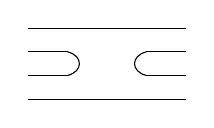
\begin{tikzpicture}
					\draw (0, 0) -- (2, 0);
					\draw (0, 0.3) -- (0.5, 0.3);
					\draw (0, 0.6) -- (0.5, 0.6);
					\draw (0.5, 0.3) .. controls (0.7, 0.35) and (0.7, 0.55) .. (0.5, 0.6);
					\draw (1.5, 0.3) -- (2, 0.3);
					\draw (1.5, 0.6) -- (2, 0.6);
					\draw (1.5, 0.3) .. controls (1.3, 0.35) and (1.3, 0.55) .. (1.5, 0.6);
					\draw (0, 0.9) -- (2, 0.9);
				\end{tikzpicture}
				\caption{Generator $U_2$ in TL$_4(\delta)$.}
				\label{fig:generator_temperley_lieb}
			\end{subfigure}
        	\end{figure}
        }
        
	\newdef{Frobenius algebra}{\index{Frobenius!algebra}
		An algebra $A$ equipped with a nondegenerate bilinear form $\eta:A\times A\rightarrow A$ satisfying the following condition for all $a,b,c\in A$:
		\begin{gather}
			\eta(ab,c)=\eta(a,bc)
		\end{gather}
	}

\subsection{Graded vector spaces}\label{section:graded_spaces}

	Similar to definition \ref{group:graded_ring} we can define the following:
	\newdef{Graded vector space}{\index{degree}\index{graded!vector space}
		Let $V_n$ be a vector space for all $n\in\mathbb{N}$. The vector space
		\begin{gather}
			\label{linalgebra:graded_vector_space}
			V = \bigoplus_{n\in\mathbb{N}} V_n
		\end{gather}
		is called a graded vector space. In fact one can replace $\mathbb{N}$ by any countable (finite or infinite) index set. For most operations however one requires the index set to be closed under addition operations. The index $n$ is often called the \textbf{degree} of the subspace $V_n$ in $V$.
	}
	
	\newdef{Graded algebra}{\index{graded!algebra}
		Let $V$ be a graded vector space with the additional structure of an algebra given by the multiplication $\star$. Then $V$ is a graded algebra if $\star$ maps $V^k\times V^l$ to $V^{k+l}$.
	}
	
	\newdef{Super vector space}{\index{super!vector space}
		A super vector space is defined as a $\mathbb{Z}_2$-graded vector space.
	}
	
	\begin{example}[Superalgebra]\index{super!algebra}\label{linalgebra:superalgebra}
		A $\mathbb{Z}_2$-graded algebra, i.e. there exists a decomposition
		\begin{gather}
			A = A_0\oplus A_1
		\end{gather}
		such that for all $i, j \mod 2$:
		\begin{gather}
			A_i\star A_j \subseteq A_{i+j}
		\end{gather}
	\end{example}
	
	\newdef{dg-algebra}{\index{dg-algebra}\label{linalgebra:dg_algebra}
		A differential graded algebra (often denoted by dg-algebra) is a graded algebra equipped with a differential of degree 1.
	}
	
	\newdef{Parity functor}{\index{parity}
		Consider the category $\mathbf{sVect}$ of super vector spaces. We can define the parity functor $\func{\Pi}{sVect}{sVect}$ as the functor which interchanges even and odd subspaces:
		\begin{align}
			(\Pi V)_0 &= V_1\\
			&\\
			(\Pi V)_1 &= V_0
		\end{align}
	}
	\newdef{Symmetric tensors}{
		Using the parity functor one can write the exterior algebra $\Lambda^\bullet(V)$ as the symmetric algebra $\text{Sym}^\bullet(\Pi V)$. In a similar way one can write the symmetric algebra on a super vector space $V=V_0\oplus V_1$ as $\text{Sym}^n(V)=\bigoplus_{p+q=n}\text{Sym}^p(V_0)\otimes\Lambda^q(V_1)$.
	}
        
\section[Linear maps]{Linear maps\footnote{Other names are \textbf{linear mapping} and \textbf{linear transformation}.}}
	
	\begin{property}
		Let $V$ be finite-dimensional $K$-vector space. Let $f:V\rightarrow V$ be a linear map. The following statements are equivalent:
        	\begin{itemize}
            		\item $f$ is injective
			\item $f$ is surjective
                	\item $f$ is bijective
		\end{itemize}
	\end{property}

	\newdef{Automorphism}{\index{automorphism}\label{linalgebra:automorphism}
		\nomenclature[S_Aut]{$\text{Aut}(V)$}{Set of automorphisms (invertible endomorphisms) on a set $V$.}
	    	An isomorphism from $V$ to $V$ is called an automorphism\footnote{In some case also called a \textbf{linear operator}, but this terminology is also used for a general linear map in operator theory (see chapter \ref{chapter:operator:algebras}).}. The set of all automorphisms  on $V$, which is in fact a group, is denoted by $\text{Aut}(V)$.
	}
    
	\newdef{General linear group\footnotemark}{\index{general linear group}
		\nomenclature[S_GL]{GL$(V)$}{General linear group: group of all automorphisms on a vector space $V$.}
		\footnotetext{This group is isomorphic to the general linear group of invertible matrices, hence the similar name and notation. (See definition \ref{linalgebra:GL_matrices})}
	    	The set of all automorphisms $f:V\rightarrow V$ is called the general linear group and denoted by GL$_K(V)$ or GL$(V)$ when the base field is clear.
	}

	\newdef{Rank}{\index{rank}\label{linalgebra:image_rank}
		The dimension of the image of a linear map is called the rank.
	}
	\newdef{Kernel}{\index{kernel}
	        The kernel of a linear map $f: V \rightarrow W$ is defined as the following subspace of $V$:
        	\begin{gather}
        		\text{ker}(f) = \{v\in V\ |\ f(v) = 0\}
	        \end{gather}
	}
	\newdef{Nullity}{\index{nullity}
		The dimension of the kernel is called the nullity.
	}
    
	\begin{theorem}
	    	A linear map $f:V\rightarrow W$ is injective if and only if $\text{ker}(f) = \{0\}$.
	\end{theorem}
	\begin{property}
	        Let $f:V\rightarrow W$ be a linear map. Let $U\leq V$. We have the following two properties of the restriction $f|_U$ of $f$ to $U$:
        	\begin{itemize}
			\item $\text{ker}\left(f|_U\right) = \text{ker}(f)\cap U$
        		\item $\text{im}\left(f|_U\right) \leq \text{im}(f)$
		\end{itemize}
	\end{property}
    
\subsection{Dimension}

        \begin{theorem}[Dimension theorem\footnotemark]\index{rank-nullity theorem}
		\footnotetext{Also called the \textbf{rank-nullity theorem}.}
		Let $f: V \rightarrow W$ be a linear map.
	        \begin{gather}
	                \label{linalgebra:dimension_theorem}
	                \dim(\text{\upshape im}(f)) + \dim(\text{\upshape ker}(f)) = \dim(\text{\upshape V})
	        \end{gather}
        \end{theorem}

        \begin{property}
		Two $K$-vector spaces are isomorphic if and only if they have the same dimension.
	\end{property}
    
\subsection{Homomorphisms}

	\newdef{Homomorphism space}{\index{morphism!of vector spaces}
		\nomenclature[S_Hom]{$\hom(V, W)$}{Set of morphisms from a set $V$ to a set $W$.}
    		Let $V,W$ be two K-vector spaces. The set of all linear maps between $V$ and $W$ is called the homomorphism space of $V$ to $W$, or shorter: the 'hom-space' of $V$ to $W$.
	    	\begin{equation}
        		\label{linalgebra:hom_space}
        		\hom_K(V, W) = \{f:V\rightarrow W\ |\ \text{f is linear}\}
		\end{equation}
	}
	\begin{theorem}\label{linalgebra:hom_dimension}
	    	If $\ V,W$ are two finite-dimensional K-vector spaces we have:
        	\begin{equation}
        		\dim\left(\emph{Hom}_K(V,W)\right) =\dim(V)\cdot\dim(W)
		\end{equation}
	\end{theorem}
        
	\newdef{Endomorphism ring}{
		\nomenclature[S_End]{$\text{End}(V)$}{Ring of endomorphisms on a set $V$.}
		The space $\hom_K(V, V)$ with the composition as multiplication forms a ring, the endomorphism ring. It is denoted by $\text{End}_K(V)$ or $\text{End}(V)$.
	}
	\begin{property}
		The endomormphism ring $\text{End}(V)$ forms a Lie algebra\footnote{See also \ref{lie:end_as_lie_algebra}.} when equipped with the commutator $[A, B] = A\circ B - B\circ A$.
	\end{property}
	
	\begin{property}[Jordan-Chevalley decomposition]\index{Jordan!decomposition}\index{semisimple!operator}\index{nilpotent}\label{linalgebra:jordan_chevalley}
		Every endomorphism $A$ can be decomposed as follows:
		\begin{equation}
			A = A_{ss} + A_n
		\end{equation}
		where
		\begin{itemize}
			\item $A_{ss}$ is \textbf{semisimple}, i.e. for every the invariant subspace of $A_{ss}$ there exists an invariant complementary subspace.
			\item $A_n$ is \textbf{nilpotent}, i.e. $\exists k\in\mathbb{N}: A_n^k = 0$.
		\end{itemize}
		Furthermore, this decomposition is unique and the endomorphisms $A_{ss}, A_n$ can be written as polynomials in $A$.
	\end{property}
    
	\newdef{Minimal polynomial}{\index{minimal polynomial}
	    	Let $f\in\text{End}(V)$ and $V$ a finite-dimensional K-vector space. The monic polynomial $\mu_f(x)$ of the lowest order such that $\mu_f(f)=0$ is called the minimal polynomial of $f$.
	}
	\begin{property}\label{linalgebra:minimal_polynomial_divisor}
		Let $f\in\text{End}(V)$. Let $\mu_f(x)$ be the minimal polynomial of $f$. Let $\varphi(x)\in K[x]$. If $\varphi(f) = 0$, then the minimal polynomial $\mu_f(x)$ divides $\varphi(x)$. 
	\end{property}
    
\subsection{Dual space}

	\newdef{Dual space}{\index{dual!space}
	    	Let $V$ be a K-vector space. The dual space $V^*$ of $V$ is the following vector space:
	    	\begin{equation}
			\label{linalgebra:dual_space}
		        V^*:=\text{Hom}_K(V, K)=\{f:V\rightarrow K\ :\ f\text{ is a linear map}\}
		\end{equation}
	}
	\newdef{Linear form}{\index{linear!form}
	    	The elements of $V^*$ are called \textit{linear forms}.
	}
	\begin{property}\label{linalgebra:dual_space_dimension}
		From theorem \ref{linalgebra:hom_dimension} it follows that $\dim(V^*) = \dim(V)$.
	\end{property}
	\begin{remark}
		If $V$ is infinite-dimensional, theorem \ref{linalgebra:dual_space_dimension} is not valid. In the infinite-dimensional case we \textbf{always} have $|V^*|>|V|$ (where we now use the cardinality instead of the dimension).
	\end{remark}
    
	\newdef{Dual basis}{
    		Let $\mathcal{B} = \{e_1, e_2, ..., e_n\}$ be a basis for a finite-dimensional K-vector space $V$. We can define a basis $\mathcal{B}^* = \{\varepsilon_1, \varepsilon_2, ..., \varepsilon_n\}$ for $V^*$, called the dual basis of $\mathcal{B}$, as follows:
    		\begin{equation}
			\label{linalgebra:dual_basis}
        		\boxed{\varepsilon_i:V\rightarrow K:\sum_{j=1}^na_ie_i\mapsto a_i}
		\end{equation}
		The relation between the basis and dual basis can also be written as:
		\begin{equation}
			\label{linalgebra:dual_basis_2}
			\varepsilon^i(e_j) = \delta^i_j
		\end{equation}
	}
    
	\newdef{Dual map}{\index{dual!map}\label{linalgebra:transpose}
		Let $f:V\rightarrow W$ be a linear map. The linear map $f^*:W^*\rightarrow V^*:\varphi\rightarrow\varphi\circ f$ is called the dual map or \textbf{transpose} of $f$.
	}
	\newnot{Transpose}{\index{transpose}
		When $V=W$ the dual map $f^*$ is often denoted by $f^T$.
	}
    
    \newdef{Natural pairing}{\index{natural!pairing}
    	The natural pairing of $V$ and its dual $V^*$ is defined as the following bilinear map:
        \begin{equation}
        	\label{linalgebra:natural_pairing}
            \langle v, v^*\rangle = v^*(v)
        \end{equation}
    }

\subsection{Convex functions}
	
	\newdef{Convex function}{\index{convex!function}
		Let $X$ be a convex subset of $V$. A function $f:X\rightarrow \mathbb{R}$ is convex if for all $x, y\in X$ and $t\in[0, 1]$:
		\begin{equation}
			f(tx + (1-t)y) \leq tf(x) + (1-t)f(y)
		\end{equation}
	}
	\begin{remark}
		For a concave function we have to turn the inequality around.
	\end{remark}
	\begin{result}
		A linear map $f:X\rightarrow\mathbb{R}$ is both convex and concave.
	\end{result}
	
	\begin{theorem}[Karamata's inequality]\index{Karamata's inequality}
		Let $I\subset\mathbb{R}$ be an interval and let $f:I\rightarrow\mathbb{R}$ be a convex function. If $(x_1, ..., x_n)$ is a tuple that majorizes $(y_1, ..., y_n)$, i.e. $\forall k\leq n$
		\begin{align}
			\sum_{i=1}^nx_i &= \sum_{i=1}^ny_i\\
			x_{(1)} + ... + x_{(k)}&\geq y_{(1)} + ... + y_{(k)}
		\end{align}
		where $x_{(i)}$ denotes the ordering\footnote{In decreasing order: $x_{(1)}\geq...\geq x_{(n)}$.} of the tuple $(x_1, ..., x_n)$. Then
		\begin{equation}
			\sum_{i=1}^nf(x_i)\geq \sum_{i=1}^nf(y_i)
		\end{equation}
	\end{theorem}

\section{Inner product}\label{linalgebra:innerproduct}

    In this section all vector spaces $V$ will be defined over $\mathbb{R}$ or $\mathbb{C}$.

\subsection{Inner product space}

    \newdef{Inner product}{\index{inner!product}
        A map $\langle\cdot|\cdot\rangle:V\times V\rightarrow\mathbb{C}$ is called an inner product on $V$ if it satisfies the following properties for all $v,w\in V$ and $\lambda\in\mathbb{C}$:
        \begin{enumerate}
            \item \textbf{Conjugate symmetry}: $\langle v|w \rangle = \langle w|v \rangle^*$,
            \item \textbf{Linearity in the first argument}: $\langle \lambda u+v|w \rangle = \lambda\langle u|w \rangle + \langle v|w \rangle$,
            \item \textbf{Nondegeneracy}: $\langle v|v \rangle = 0 \iff v = 0$, and
            \item \textbf{Positive-definiteness}: $\langle v|v \rangle \geq 0$.
        \end{enumerate}
    }
    \begin{remark}\index{Hermitian!form}\label{linalgebra:NDH_form}
        Inner products are special cases of \textbf{nondegenerate Hermitian forms} which do not satisfy the positive-definiteness property (these often occur when working over $\mathbb{C}$).
    \end{remark}

    \begin{result}\index{sesquilinear}
        The first two properties have the result of conjugate linearity in the second argument:
        \begin{gather}
            \langle f|\lambda g + \mu h \rangle = \overline{\lambda}\langle f|g \rangle + \overline{\mu}\langle f|h \rangle
        \end{gather}
        Therefore these two properties together are often combined into a \textbf{sesquilinearity} property. When the underlying field is restricted to $\mathbb{R}$, such that the conjugate symmetry property is replaced by symmetry, the inner product becomes a bilinear form.
    \end{result}

    \newdef{Inner product space\footnotemark}{
        \footnotetext{Sometimes called a \textbf{pre-Hilbert space}.}
        A vector space equipped with an inner product $\langle\cdot|\cdot\rangle$.
    }

    \newdef{Metric dual\footnotemark}{
        \footnotetext{See also Definition \ref{riemann:flat_map}.}
        Using the inner product (or any other nondegenerate Hermitian form) one can define the metric dual of a vector $v$ by the following map:
        \begin{gather}
            \label{linalgebra:metric_dual}
            L:V\rightarrow V^*:v\mapsto \langle v|\cdot \rangle.
        \end{gather}
    }
    \newdef{Adjoint operator}{\index{adjoint}\index{Hermitian}\index{self-adjoint}\label{linalgebra:adjoint_operator}
        Let $A$ be a linear operator on $V$. The (\textbf{Hermitian}) adjoint of $A$ is defined as the linear operator $A^\dag$ that satisfies
        \begin{gather}
            \langle A^\dag v|w\rangle = \langle v|Aw\rangle
        \end{gather}
        for all $v,w\in V$. Alternatively, one can define the adjoint using the transpose and metric dual as follows:
        \begin{gather}
            A^\dag = L^{-1} \circ A^T \circ L.
        \end{gather}
        If $A=A^\dag$, then A is said to be \textbf{Hermitian} or \textbf{self-adjoint}. (In Chapter \ref{chapter:normed_spaces} a distinction will be made between these two notions.)
    }
    \begin{result}
        The Hermitian adjoint of a complex matrix $A\in\mathbb{C}^{m\times n}$ is given by
        \begin{gather}
            A^\dag = \overline{A}^T,
        \end{gather}
        where $\overline{A}$ denotes the complex conjugate of $A$ and $A^T$ the transpose of $A$.
    \end{result}

\subsection{Orthogonality}\label{linalgebra:section:orthogonality}

    \newdef{Orthogonal}{\index{orthogonal}\label{linalgebra:orthogonal}
        Consider two vectors $v,w\in V$ in an inner product space. These vectors are said to be orthogonal, denoted by $v\perp w$,  if they obey the following relation:
        \begin{gather}
            \langle v|w \rangle = 0.
        \end{gather}
        An \textbf{orthogonal system} is a collection of vectors, none of them equal to 0, that are mutually orthogonal.
    }
    \begin{property}
        Orthogonal systems are linearly independent.
    \end{property}

    \newdef{Orthonormal}{\index{orthonormal}\label{linalgebra:orthonormal}
        A collection of vectors $S$ is said to be orthonormal if it forms an orthogonal system and if all the elements $v\in S$ obey the following relation:
        \begin{gather}
            \langle v|v \rangle = 1.
        \end{gather}
    }
    \newdef{Orthogonal complement}{\index{complement}\label{linalgebra:orthogonal_complement}
        Let $W$ be a subspace of an inner product space $V$. The orthogonal complement of $W$ is defined as the following subspace:
        \begin{gather}
            W^\perp := \{v\in V\mid\forall w\in W:\langle v|w\rangle = 0\}.
        \end{gather}
    }
    \sremark{$W^\perp$ is pronounced as 'W-perp'.}

    \begin{property}[Complements]
        Let $V$ be a finite-dimensional inner product space. The orthogonal complement $W^\perp$ is a complementary subspace to $W$, i.e. $W\oplus W^\perp=V$.
    \end{property}
    \begin{result}\label{linalgebra:perp_of_perp}
        Let $W\leq V$ where $V$ is a finite-dimensional inner product vector space. Taking orthogonal complements defines an involution:
        \begin{gather}
            (W^\perp)^\perp = W.
        \end{gather}
    \end{result}

    \newdef{Orthogonal projection}{\index{projection}\label{linalgebra:orthogonal_projection}
        Let $V$ be a finite-dimensional inner product vector space and consider a subspace $W\leq V$. Consider a vector $w\in W$ and let $\{w_1, \ldots, w_k\}$ be an orthonormal basis of $W$. The projections of $v\in V$ on $W$ and $w\in W$ are defined as follows:
        \begin{align}
            \text{proj}_W(v) &:= \sum_{i=1}^k\langle v|w_i \rangle w_i\\
            \text{proj}_w(v) &:= \stylefrac{\langle v|w \rangle}{\langle w|w \rangle}w.
        \end{align}
    }
    \begin{property}
        Orthogonal projections satisfy the following conditions:
        \begin{itemize}
            \item $\forall w\in W:\text{proj}_W(w) = w$, and
            \item $\forall u\in W^\perp:\text{proj}_W(u) = 0$.
        \end{itemize}
    \end{property}

    \newmethod{Gram-Schmidt orthonormalization}{\label{linalgebra:inner_product:gram_schmidt}
        Let $\{u_i\}_{i\leq n}$ be a set of linearly independent vectors. An orthonormal set $\{e_i\}_{i\leq n}$ can be constructed out of $\{u_i\}_{i\leq n}$ using the following procedure:
        \begin{enumerate}
            \item Orthogonalization:
                \begin{gather}
                    \begin{aligned}
                        w_1& = u_1&\\
                        w_2& = u_2 - \stylefrac{\langle u_2|w_1\rangle}{||u_2||^2}w_1&\\
                        &\vdots&\\
                        w_n& = u_n - \sum_{i=1}^{n-1}\stylefrac{\langle u_n|w_i\rangle}{||u_n||^2}w_i&
                    \end{aligned}
                \end{gather}
            \item Normalization:
                \begin{gather}
                    \begin{aligned}
                        e_1& = \stylefrac{w_1}{||w_1||}&\\
                        e_2& = \stylefrac{w_2}{||w_2||}&\\
                        &\vdots&\\
                        e_n& = \stylefrac{w_n}{||w_n||}&
                    \end{aligned}
                \end{gather}
        \end{enumerate}
    }

    \newdef{Householder transformation}{\index{Householder transformation}\label{linalgebra:householder_transformation}
        Let $v$ be an element of an inner product space $V$. The Householder transformation generated by $v$ is given by the linear map
        \begin{gather}
            \sigma_v:V\rightarrow V:w\mapsto w - 2\frac{\langle w|v \rangle}{\langle v|v \rangle}v.
        \end{gather}
        This transformation amounts to a reflection in the hyperplane orthogonal to $v$.
    }

    \newdef{Angle}{\index{angle}\label{linalgebra:angle}
        Let $v,w$ be elements of an inner product space $V$. The angle $\theta$ between $v$ and $w$ is defined by the following formula:
        \begin{gather}
            \cos\theta := \stylefrac{\langle v|w \rangle}{||v||||w||}.
        \end{gather}
    }
\section{Matrices}
	
	\begin{notation}\label{linalgebra:matrix_set}
	        The set of all $m\times n$-matrices defined over the field $K$ is denoted by $M_{m,n}(K)$. If $m=n$, the set is denoted by $M_n(K)$.
	\end{notation}
	
	\begin{property}[Dimension]\index{dimension}\label{linalgebra:dimension_of_matrix_space}
		The dimension of $M_{m,n}(K)$ as a vector space is $mn$.
	\end{property}
    
	\newdef{Trace}{\index{trace}\label{linalgebra:trace}
	        Let $A = (a_{ij})\in M_n(K)$. We define the trace of $A$ as follows:
    		\begin{gather}
			\text{tr}(A) = \sum_{i=1}^na_{ii}
		\end{gather}
	}
	\begin{property}\label{linalgebra:trace_commutative}
		Let $A, B\in M_n(K)$. The trace satisfies the following properties:
	        \begin{enumerate}
        		\item $\text{tr}:M_n(K)\rightarrow K$ is a linear map
			\item $\text{tr}(AB) = \text{tr}(BA)$
			\item $\text{tr}(AB) \neq \text{tr}(A)\text{tr}(B)$
        		\item $\text{tr}(A^T) = \text{tr}(A)$
		\end{enumerate}
	\end{property}
    
	\newformula{Hilbert-Schmidt norm\footnotemark}{\index{Frobenius!norm}\index{Hilbert-Schmidt norm}
    		\footnotetext{Also called the \textbf{Frobenius norm}.}
    		The Hilbert-Schmidt norm is given by the following formula:
	        \begin{gather}
        		\label{linalgebra:hilbert_schmidt_norm}
        		||A||^2_{HS} = \sum_{i, j}|A_{ij}|^2 = \text{tr}(A^\dag A)
	        \end{gather}
        	If one identifies $M_{n}(\mathbb{C})$ with $\mathbb{C}^{2n}$ then this norm equals the standard Hermitian norm.
	}

	\newformula{Hadamard product}{\index{Hadamard!product}
    		The Hadamard product of two matrices $A, B\in M_{m\times n}(K)$ is defined as the entry-wise product:
        	\begin{gather}
        		(A\circ B)_{ij} = A_{ij}B_{ij}
        	\end{gather}
	}
    
	\newdef{General linear group}{\index{general linear group}\label{linalgebra:GL_matrices}
		\nomenclature[S_GLn]{GL$(n,K)$}{General linear group: group of all invertible $n$-dimensional matrices over the field $K$.}
	        The set of invertible matrices is called the general linear group and is denoted by GL$_n(K)$ or GL$(n, K)$.
	}
	\begin{property}
		For all $A\in\text{GL}_n(K)$ we have:
	        \begin{itemize}
			\item $A^T\in\text{GL}_n(K)$
		        \item $\left(A^T\right)^{-1}=\left(A^{-1}\right)^T$
		\end{itemize}
	\end{property}
    
	\begin{property}\label{linalgebra:dim_columns_rows}
		Let $A\in M_{m,n}(K)$. Denote the set of columns as $\{A_1, A_2, ..., A_n\}$ and the set of rows as $\{R_1, R_2, ..., R_m\}$. The set of columns is a subset of $K^m$ and the set of rows is a subset of $K^n$ and as such we can define their span. These spaces satisfy the following property:
		\begin{gather}
			\dim(\text{span}(A_1, ..., A_n)) = \dim(\text{span}(R_1, ..., R_m))
		\end{gather}
	\end{property}
	
	\newdef{Rank}{\index{rank}
		Using the invariance relation from previous property we can define the rank of a matrix $A\in M_{m,n}(K)$ as follows:
		\begin{gather}
			\label{linalgebra:matrix_rank}
        		\text{rk}(A) := \dim(\text{span}(A_1, ..., A_n)) \overset{\ref{linalgebra:dim_columns_rows}}{=} \dim(\text{span}(R_1, ..., R_m))
		\end{gather}
	}
    
	\begin{property}\label{linalgebra:rank_properties}
	        The rank of a matrix has the following properties:
        	\begin{enumerate}
			\item $\text{rk}(AC)\leq\text{rk}(A)$ and $\text{rk}(AC)\leq\text{rk}(C)$
        		\item $\text{rk}(BC)=\text{rk}(C)$
		        \item $\text{rk}(BD)=\text{rk}(D)$
		\end{enumerate}
		where $A\in M_{m,n}(K)$, $B\in\text{GL}_n(K)$, $C\in M_{n,r}(K)$ and $D\in M_{r,n}(K)$.
	\end{property}
	\begin{property}\label{linalgebra:dim_matrix_left_multiplication}
	        Let $A\in M_{m,n}(K)$. We first define the following linear map:
        	\begin{gather}
			\label{linalgebra:matrix_left_multiplication}
        		L_A:K^n\rightarrow K^m:v\mapsto Av
		\end{gather}
	        This map has the following properties:
        	\begin{enumerate}
        		\item $\text{im}(L_A) = \text{span}(A_1, ..., A_n)$
			\item $\dim(\text{im}(L_A))=\text{rk}(A)$
		\end{enumerate}
	\end{property}
	\sremark{The second property is a direct consequence of the first one together with definition \ref{linalgebra:matrix_rank}.}
    
\subsection{System of equations}

	\begin{property}\label{linalgebra:matrix_and_equations}
	        Let $AX=w$ with $A\in M_{m,n}(K)$, $w\in K^m$ and $X\in K^n$ be a system of $m$ equations in $n$ variables. Let $L_A$ be the linear map as defined in equation \ref{linalgebra:matrix_left_multiplication}. We then have the following properties:
        	\begin{enumerate}
			\item The system is false if and only if $w\not\in\text{im}(L_A)$.
        		\item If the system is not false, the solution set is an affine space. If $v_0\in K^n$ is a solution, then the solution set is given by: $L_A^{-1}(w)=v_0+\text{ker}(L_A)$.
		        \item If the system is homogeneous ($AX=0$), then the solution set is equal to $\text{ker}(L_A)$.
		\end{enumerate}
	\end{property}
	\begin{property}[Uniqueness]\label{linalgebra:rank_unique_solution}
	        Let $AX=w$ with $A\in M_n(K)$ be a system of $n$ equations in $n$ variables. If $\text{rk}(A)=n$, then the system has a unique solution.
	\end{property}
	
	\newformula{Cramer's rule}{\index{Cramer}
    		Let $AX = w$ be a system of linear equations where the matrix $A$ has a nonzero determinant. Then Cramer's rule gives a unique solution where the unknowns are given by;
		\begin{gather}
			\label{linalgebra:cramers_rule}
			X_i = \stylefrac{\det(A_i)}{\det(A)}
		\end{gather}
		where $A_i$ is the matrix obtained by replacing the $i^{th}$ column of $A$ by the column matrix $w$.
	}
    
\subsection{Coordinates and matrix representations}

        \newdef{Coordinate vector}{\label{linalgebra:coordinate_vector}
        	Let $\mathcal{B} = \{b_1, ..., b_n\}$ be a basis of $V$. Let $v\in V$ such that $v=\sum_{i=1}^n\lambda_ib_i$. We define the coordinate vector of $v$ with respect to $\mathcal{B}$ as $(\lambda_1, ..., \lambda_n)^T$. The $\lambda_i$'s are called the \textbf{coordinates} of $v$ with respect to $\mathcal{B}$.
        }
        \newdef{Coordinate isomorphism}{\label{linalgebra:coordinate_isomorphism}
        	With the previous definition in mind we can define the coordinate isomorphism of $v$ with respect to $\mathcal{B}$ as follows:
        	\begin{gather}
			\boxed{\beta:V\rightarrow K^n:\sum_{i=1}^n\lambda_ib_i\mapsto(\lambda_1, ..., \lambda_n)^T}
		\end{gather}
        }
        
        \newdef{Matrix representation}{\label{linalgebra:matrix_representation}
        	Let $V$ be an $n$-dimensional K-vector space and $W$ an $m$-dimensional K-vector space. Let $f:V\rightarrow W$ be a linear map. Let $\mathcal{B}=\{b_1, ..., b_n\}, \mathcal{C} = \{c_1, ..., c_m\}$ be a basis for $V$, respectively $W$. The matrix representation of $f$ with respect to $\mathcal{B}$ and $\mathcal{C}$ can be derived as follows: For every $j\in\{1, ..., n\}$ we can write $f(b_j) = \sum_{i=1}^ma_{ij}c_i$, so with this in mind we can define the matrix $(a_{ij})\in M_{m,n}(K)$ as the matrix represenation of $f$.
        }
        \newnot{Matrix representation of a linear map}{
        	The matrix representation of $f$ with respect to $\mathcal{B}$ and $\mathcal{C}$ is denoted by $A_{f, \mathcal{B}, \mathcal{C}}$.
        }
        
        \newmethod{Construction of a matrix representation}{\label{linalgebra:method:matrix_representation}
        	From definition \ref{linalgebra:matrix_representation} we can see that $j$-th column of $A_{f, \mathcal{B}, \mathcal{C}}$ coincides with the coordinate vector of $f(b_j)$ with respect to $\mathcal{C}$. We use this relation to construct $A_{f, \mathcal{B}, \mathcal{C}}$ by writing for every $j\in\{1, ..., n\}$ the coordinate vector of $f(b_j)$ in the $j$-th column.
        }
        
        \begin{theorem}\label{linalgebra:theorem:matrix_representation}
		Let $(\lambda_1, ..., \lambda_n)^T$ be the coordinate vector of $v\in V$ with respect to $\mathcal{B}$. Let $(\mu_1, ..., \mu_m)^T$ be the coordinate vector of $f(v)$ with respect to $\mathcal{C}$. Then the following relation holds:
            	\begin{gather}
			\left(
			\begin{array}{c}
				\mu_1\\
				\vdots\\
				\mu_m
			\end{array}\right)
	                = A_{f, \mathcal{B}, \mathcal{C}}
        	        \left(\begin{array}{c}
				\lambda_1\\
				\vdots\\
				\lambda_n
			\end{array}\right)
		\end{gather}
	\end{theorem}
        
        \begin{theorem}\label{linalgebra:theorem:map_matrix_link}
		For every matrix $A\in M_{m,n}(K)$ there exists a linear map $f:V\rightarrow W$ such that $A_{f, \mathcal{B}, \mathcal{C}} = A$.
	\end{theorem}
        On the other hand we also have the following theorem:
        \begin{theorem}
		Let $f:K^n\rightarrow K^m$ be a linear map. There exists a matrix $A\in M_{m,n}(K)$ such that $f=L_A$.
	\end{theorem}
        \begin{theorem}
		Let $\beta$ and $\gamma$ be the coordinate isomorphisms with respect to respectively $\mathcal{B}$ and $\mathcal{C}$. From theorem \ref{linalgebra:theorem:matrix_representation} it follows that:
        	\begin{gather}
			\gamma(f(v)) = A_f\cdot\beta(v)
		\end{gather}
        	or alternatively
        	\begin{gather}
			\gamma\circ f = L_{A_f}\circ\beta
		\end{gather}
	\end{theorem}
        
        \begin{theorem}\label{linalgebra:theorem:matrix_composition_hom}
	        The map $\text{Hom}_K(V,W)\rightarrow M_{m,n}(K):f\mapsto A_f$ is an isomorphism and for every $f\in\text{Hom}_K(V,W)$ and $g\in \text{Hom}_K(W,U)$ we have:
		\begin{gather}
			A_{g\circ f} = A_gA_f
		\end{gather}
	\end{theorem}
	
	\begin{theorem}\label{linalgebra:theorem:matrix_composition_end}
	        The map $\text{End}_K(V)\rightarrow M_n(K):f\mapsto A_{f, \mathcal{B}, \mathcal{B}}$ is an isomorphism and for every $f,g\in\text{End}_K(V)$ we have:
        	\begin{gather}
			A_{g\circ f} = A_gA_f
		\end{gather}
	\end{theorem}
	
        \begin{theorem}\label{linalgebra:matrix_invertable_map}
	        Let $f\in\text{End}_K(V)$. Let $A_f$ be the corresponding matrix representation. The linear map $f$ is invertible if and only if $A_f$ is invertible. Furthermore, if $A_f$ is invertible, we have that \[\left(A_f\right)^{-1} = A_{f^{-1}}\] In other words, the following map is an isomorphism\footnotemark:
	        \begin{gather}
	        	\text{GL}_K(V)\rightarrow\text{GL}_n(K):f\mapsto A_f
	        \end{gather}
	        \footnotetext{Follows from theorem \ref{linalgebra:theorem:matrix_composition_end}.}
	\end{theorem}
        \remark{The sets GL$_K(V)$ and GL$_N(K)$ are groups. So the previous theorem states that the map $f\mapsto A_f$ is a group isomorphism.}
        
        \begin{theorem}
		Let $V = K^n$. Let $f\in V^*$. From construction \ref{linalgebra:method:matrix_representation} it follows that $A_f = (f(e_1), ..., f(e_n))\in M_{1,n}(K)$ with respect to the standard basis of $V$. This combined with theorem \ref{linalgebra:theorem:matrix_representation} gives:
	        \begin{gather}
			f(\lambda_1, ..., \lambda_n)^T = (f(e_1), ..., f(e_n))(\lambda_1, ..., \lambda_n)^T = \sum_{i=1}^nf(e_i)\lambda_i
		\end{gather}
        	or alternatively with $\{\varepsilon_1, ..., \varepsilon_n\}$ the dual basis to the standard basis of $V$:
	        \begin{gather}
        	    	\label{linalgebra:map_in_function_of_dual_basis}
			\boxed{f = \sum_{i=1}^nf(e_i)\varepsilon_i}
		\end{gather}
	\end{theorem}
        
        \begin{theorem}
		Let $f:V\rightarrow W$ be a linear map. Let $f^*:W^*\rightarrow V^*$ be the corresponding dual map. If $A_f$ is the matrix representation of $f$ with respect to $\mathcal{B}$ and $\mathcal{C}$, then the transpose $A_f^T$ is the matrix representation of $f^*$ with respect to the dual basis of $\mathcal{C}$ and the dual basis of $\mathcal{B}$.
	\end{theorem}
        
\subsection{Coordinate transforms}
        
        \newdef{Transition matrix}{\label{linalgebra:transition_matrix}
        	Let $\mathcal{B} = \{b_1, ..., b_n\}$ and $\mathcal{B}' = \{b_1', ..., b_n'\}$ be two bases of $V$. Every element of $\mathcal{B}'$ can be written as a linear combination of elements in $\mathcal{B}$:
        	\begin{gather}
        		b_j' = q_{1j}b_1 + ... + q_{nj}b_n
        	\end{gather}
	        The matrix $Q = (q_{ij})\in M_n(K)$ is called the transition matrix from the 'old' basis $\mathcal{B}$ to the 'new' basis $\mathcal{B}'$.}
        
        \begin{theorem}\label{linalgebra:theorem:transition_matrix}
		Let $\mathcal{B}, \mathcal{B}'$ be two basis of $V$. Let $Q$ be the transition matrix from $\mathcal{B}$ to $\mathcal{B}'$. We find the following statements:
	        \begin{enumerate}
			\item Let $\mathcal{C}$ be an arbitrary basis of $V$ with $\gamma$ the corresponding coordinate isomorphism. Define the following matrices:
        	        	\[
        	        		B=(\gamma(b_1), ..., \gamma(b_n))\quad\text{and}\quad B'=(\gamma(b_1'), ..., \gamma(b_n'))
        	        	\]
		                Then $BQ = B'$.
			\item $Q\in\text{GL}_n(K)$ and $Q^{-1}$ is the transition matrix from $\mathcal{B}'$ to $\mathcal{B}$.
                	\item Let $v\in V$ with $(\lambda_1, ..., \lambda_n)^T$ the coordinate vector with respect to $\mathcal{B}$ and $(\lambda_1', ..., \lambda_n')^T$ the coordinate vector with respect to $\mathcal{B}'$. Then:
                	\[
		                Q\left(
				\begin{array}{c}
					\lambda_1'\\
                			\vdots\\
			        	\lambda_n'
				\end{array}
                        	\right)
                        	=
		                \left(
                		\begin{array}{c}
					\lambda_1\\
                			\vdots\\
			        	\lambda_n
				\end{array}
                        	\right)
				\quad\text{and}\quad
                        	\left(
                        	\begin{array}{c}
					\lambda_1'\\
                        		\vdots\\
			        	\lambda_n'
				\end{array}
		                \right)
                	        =
                	        Q^{-1}\left(
                	        \begin{array}{c}
					\lambda_1\\
                		        \vdots\\
			                \lambda_n
				\end{array}
                        	\right)
			\]
		\end{enumerate}
	\end{theorem}
        
	\begin{theorem}\label{linalgebra:theorem:transition_matrix_representation}
        	Let $V,W$ be two finite-dimensional K-vector spaces. Let $\mathcal{B}, \mathcal{B}'$ be two bases of $V$ and $\mathcal{C}, \mathcal{C}'$ two bases of $W$. Let $Q, P$ be the transition matrices from $\mathcal{B}$ to $\mathcal{B}'$ and from $\mathcal{C}$ to $\mathcal{C}'$ respectively. Let $A=A_{f, \mathcal{B}, \mathcal{C}}$ and $A' = A_{f, \mathcal{B}', \mathcal{C}'}$. Then:
	        \begin{gather}
        	    	A' = P^{-1}AQ
        	\end{gather}
	\end{theorem}
        \begin{result}
		Let $f\in \text{End}_K(V)$ and let $Q$ be the transition matrix. From theorem \ref{linalgebra:theorem:transition_matrix_representation} it follows that:
            	\begin{gather}
	            	A'=Q^{-1}AQ
        	\end{gather}
	\end{result}

        \newdef{Matrix conjugation}{\index{conjugacy class}\index{matrix!conjugation}\label{linalgebra:conjugacy_class}
        	Let $A\in M_n(K)$. The set
        	\begin{gather}
	            	\{Q^{-1}AQ\ |\ Q\in\text{GL}_n(K)\}
        	\end{gather}
	        is called the conjugacy class\footnotemark\ of $A$. Another name for conjugation is \textbf{similarity transformation}.
        	\footnotetext{This is the general definition of conjugacy classes for groups. Furthermore, these classes induce a partitioning of the group.}
	}
        \begin{remark}
        	If $A$ is a matrix representation of a linear operator $f$, then the conjugacy class of $A$ consists out of every possible matrix representation of $f$.
        \end{remark}
        
        \begin{property}
        	From property \ref{linalgebra:trace_commutative} it follows that the trace of a matrix is invariant under similarity transformations:
        	\begin{gather}
            		\label{linalgebra:trace_invariance}
            		\boxed{\text{tr}(Q^{-1}AQ) = \text{tr}(A)}
	        \end{gather}
        \end{property}
        
        \newdef{Matrix congruence}{\index{matrix!congruence}\label{linalgebra:matrix_congruence}
        	Let $A, B\in M_n(K)$. If there exists a matrix $P$ such that
	        \begin{gather}
        	    	A = P^TBP
        	\end{gather}
	        then the matrices are said to be congruent.
        }
        \begin{property}
        	Every matrix congruent to a symmetric matrix is also symmetric.
        \end{property}
        
        \begin{theorem}\label{linalgebra:theorem:orthogonal_transition_matrix}
        	Let $(V, \langle .|. \rangle)$ be an inner-product space defined over $\mathbb{R}$ (or $\mathbb{C}$). Let $\mathcal{B}, \mathcal{B}'$ be two orthonormal bases of $V$ and let $Q$ be the transition matrix. Then $Q$ is orthogonal:
        	\begin{gather}
	        	Q^TQ = \mathbbm{1}_n
	        \end{gather}
	\end{theorem}

\subsection{Determinant}

    	\newdef{Minor}{
        	The $(i, j)$-th minor of $A$ is defined as:\[\det(A_{ij})\] where $A_{ij}\in M_{n-1}(K)$ is the matrix obtained by removing the $i$-th row and the $j$-th column from $A$.
	}
        \newdef{Cofactor}{
        	The cofactor $\alpha_{ij}$ of the matrix element $a_{ij}$ is equal to:\[(-1)^{i+j}\det(A_{ij})\]where $\det(A_{ij})$ is the minor as previously defined.
	}
        \newdef{Adjugate matrix}{\label{linalgebra:adjugate_matrix}
	        The adjugate matrix of $A\in M_n(K)$ is defined as follows:
	       	\begin{gather}
	            	\text{adj}(A) := \left(
	                \begin{array}{cccc}
				\alpha_{11}&\alpha_{21}&\dotsm&\alpha_{n1}\\
		                \alpha_{12}&\alpha_{22}&\dotsm&\alpha_{n2}\\
		                \vdots&\vdots&\vdots&\vdots\\
		                \alpha_{1n}&\alpha_{2n}&\dotsm&\alpha_{nn}\\
			\end{array}
        	        \right)
		\end{gather}
        	or shorter: $\text{adj}(A) = (\alpha_{ij})^T$.
        }
        \begin{remark*}
		It is important to notice that we have to transpose the matrix after the elements have been replaced by their cofactor.
	\end{remark*}
        
        \begin{property}\label{linalgebra:determinant_properties}
	        Let $A,B\in M_n(K)$. Denote the columns of $A$ as $A_1, \dotso, A_n$. We have the following properties of the determinant:
	        \begin{enumerate}
			\item $\det(A^T) = \det(A)$
	                \item $\det(AB) = \det(BA) = \det(A)\det(B)$
	                \item $\det(A_1, \dotso, A_i+\lambda A_i', \dotso, A_n) = \det(A_1, \dotso, A_i, \dotso, A_n) + \lambda\det(A_1, \dotso,A_i', \dotso, A_n)$ for all $A_i,A_i'\in M_{n,1}(K)$.
	                \item If two columns of $A$ are equal then $\det(A) = 0$.
	                \item $\det(A_{\sigma(1)},\dotso,A_{\sigma(n)}) = \text{sgn}(\sigma)\det(A_1,\dotso,A_n)$
	                \item The determinant can be evaluated as follows:
	                	\begin{gather}
					\det(A) = \sum_{i=1}^n(-1)^{i+k}a_{ik}\det(A_{ik})
				\end{gather}
		\end{enumerate}
		\end{property}
        
	\begin{theorem}\label{linalgebra:theorem:rank_det_equivalence}
        	Let $A\in M_n(K)$, the following statements are equivalent:
        	\begin{enumerate}
			\item $\det(A) \neq 0$
        	        \item $\text{rk}(A) = n$
        	        \item $A\in\text{GL}_n(K)$
		\end{enumerate}
	\end{theorem}
        \begin{theorem}\label{linalgebra:theorem:adjugate_matrix}
            For all $A\in M_n(K)$ we find $A\text{adj}(A) = \text{adj}(A)A = \det(A)I_n$.
	\end{theorem}
        \begin{formula}\label{linalgebra:theorem:determinant_inverse}
	        For all $A\in\text{GL}_n(K)$ we find:
		\begin{gather}
            		A^{-1} = \det(A)^{-1}\ \text{adj}(A)
            	\end{gather}
	\end{formula}
        
        An alternative definition of a $k\times k$-minor is: 
        \begin{definition}
		Let $A\in M_{m,n}(K)$ and $k\leq\min(m, n)$. A $k\times k$-minor of $A$ is the determinant of a $k\times k$-partial matrix obtained by removing $m-k$ rows and $n-k$ columns from $A$.
	\end{definition}
        \begin{theorem}
		Let $A\in M_{m,n}(K)$ and $k\leq\min(m, n)$. We find that $\text{rk}(A)\geq k$ if and only if $A$ contains a non-zero $k\times k$-minor.
	\end{theorem}
        
        \begin{theorem}
		Let $f\in\textup{End}_K(V)$. The determinant of the matrix representation of $f$ is invariant under basis transformations.
	\end{theorem}
	
        \newdef{Determinant of a linear operator}{\index{determinant}\label{linalgebra:operator_determinant}
        	The previous theorem allows us to unambiguously define the determinant of $f\in\textup{End}_K(V)$ as follows:
        	\[\det(f) := \det(A)\]
		where $A$ is some matrix representation of $f$.
        }

\subsection{Characteristic polynomial}

    	\begin{definition}[Characteristic polynomial\footnotemark]\index{characteristic!polynomial}\label{linalgebra:characteristic_polynomial}
		Let $V$ be a finite-dimensional K-vector space. Let $f\in \text{End}_K(V)$ be a linear operator with the matrix representation $A$ (with respect to some arbitrary basis). We then find:
		\begin{gather}
                	\chi_f(x) := \det(x\mathbbm{1}_n - A) \in K[x]
		\end{gather}
		is a monic polynomial of degree $n$ in the variable $x$ and the polynomial does not depend on the choice of basis.
		\footnotetext{This polynomial can also be used directly for a matrix $A$ as theorem \ref{linalgebra:theorem:map_matrix_link} matches every matrix $A$ with some linear operator $f$.}
	\end{definition}
        
        \begin{definition}[Characteristic equation\footnotemark]\index{characteristic!equation}
        	\footnotetext{This equation is sometimes called the \textbf{secular equation}.}
		The following equation is called the characteristic equation of $f$:
	        \begin{gather}
            		\label{linalgebra:characteristic_equation}
			\boxed{\chi_f(x) = 0}
		\end{gather}
	\end{definition}
        
        \begin{formula}\label{linalgebra:parts_of_characteristic_polynomial}
        	Let $A=(a_{ij})\in M_n(K)$ with characteristic polynomial: \[\chi_A(x) = x^n + c_{n-1}x^{n-1} + \dotso + c_1x + c_0\] We then have the following result:
        	\begin{gather}
			\begin{cases}
				c_0 = (-1)^n\det(A)\\
				c_{n-1} = -\text{tr}(A)
			\end{cases}
		\end{gather}
	\end{formula}
        
        \begin{theorem}[Cayley-Hamilton]\index{Cayley-Hamilton theorem}\label{linalgebra:cayley_hamilton}\
	        \begin{enumerate}
			\item Let $A\in\text{M}_n(K)$ with characteristic polynomial $\chi_A(x)$. We find the following relation:
		                \begin{gather}
					\chi_A(A) = A^n + \sum_{i=1}^{n-1}c_iA^i= 0
				\end{gather}
	                \item Let $f\in\textup{End}_K(V)$ with characteristic polynomial $\chi_f(x)$. We find that
		                \begin{gather}
					\chi_f(f) = f^n + \sum_{i=1}^{n-1}c_if^i= 0
				\end{gather}
		\end{enumerate}
	\end{theorem}
        \begin{result}
		From theorem \ref{linalgebra:minimal_polynomial_divisor} and the Cayley-Hamilton theorem it follows that the minimal polynomial $\mu_f(x)$ is a divisor of the characteristic polynomial $\chi_f(x)$.
	\end{result}
        
\subsection{Linear groups}\label{linalgebra:section:linear_groups}
        
        \newdef{Elementary matrix}{\label{linalgebra:elementary_matrix}An elementary matrix is a matrix of the following form:
        	\[\left(
                \begin{array}{cccc}
			1&0&\dotsm&0\\
        	        0&1&c_{ij}&0\\
                	\vdots&\vdots&\ddots&\vdots\\
	                0&0&\vdots&1
		\end{array}
		\right),
        	\left(
                \begin{array}{cccc}
			1&0&\dotsm&0\\
                	0&1&\dotsm&0\\
	                \vdots&c_{ij}&\ddots&\vdots\\
        	        0&0&\vdots&1
		\end{array}
		\right),\dotso\]
		i.e. equal to the sum of an identity matrix and a multiple of a matrix unit $U_{ij}, i\neq j$.
        }
        \newnot{Elementary matrix}{$E_{ij}(c)$ is the elementary matrix with element $c$ on the $i,j$-th position.}
        \begin{property}
        	We have the following property:
		\begin{gather}
			\det(E_{ij}(c)) = 1
		\end{gather}
		which implies that $E_{ij}(c)\in\text{GL}_n(K)$.
	\end{property}
        \begin{property}
		We find the following results concerning the multiplication by an elementary matrix:
	        \begin{enumerate}
			\item Left multiplication by an elementary matrix $E_{ij}(c)$ comes down to replacing the $i$-th row of the matrix with the $i$-th row plus $c$ times the $j$-th row.
                	\item Right multiplication by an elementary matrix $E_{ij}(c)$ comes down to replacing the $j$-th column of the matrix with the $j$-th column plus $c$ times the $i$-th column.
		\end{enumerate}
		\end{property}
        
        \begin{theorem}\label{linalgebra:theorem:elementary_matrices}
		Every matrix $A\in\text{GL}_n(K)$ can be written in the following way: \[A = SD\] where $S$ is a product of elementary matrices and $D=\text{diag}(1,\dotso,1,\det(A))$.
	\end{theorem}
        
        \newdef{Special linear group}{\label{linalgebra:special_linear_group}
        	The following subset of GL$_n(K)$ is called the special linear group:
		\begin{gather}
			\text{SL}_n(K) = \{A\in \text{GL}_n(K)\ |\ \det(A) = 1\}
		\end{gather}
        }
        \begin{theorem}
		Every $A\in\text{SL}_n(K)$ can be written as a product of elementary matrices.\footnote{This follows readily from theorem \ref{linalgebra:theorem:elementary_matrices}.}
	\end{theorem}
        
        \newdef{Orthogonal group}{\label{linalgebra:orthogonal_group}The orthogonal and special orthogonal group are defined as follows:
        	\begin{align}
			\text{O}_n(K) &= \{A\in \text{GL}_n(K)\ |\ AA^T = A^TA = I_n\}\nonumber\\
			\text{SO}_n(K) &= \text{O}_n(K)\cap \text{SL}_n(K)\nonumber
		\end{align}
        }
        \begin{property}\label{linalgebra:con_equivalence}
        	For orthogonal matrices, conjugacy \ref{linalgebra:conjugacy_class} and congruency \ref{linalgebra:matrix_congruence} are equivalent.
        \end{property}
        
        \newdef{Unitary group}{\label{linalgebra:unitary_group}\index{involution}
        	The unitary and special unitary group are defined as follows:
        	\begin{align}
			\text{U}_n(K, \sigma) &= \{A\in \text{GL}_n(K)\ |\ A\overline{A}^T = \overline{A}^TA = I_n\}\nonumber\\
			\text{SU}_n(K, \sigma) &= \text{U}_n(K)\cap \text{SL}_n(K)\nonumber
		\end{align}
		where $\sigma$ denotes the \textit{involution}\footnotemark\ $a^\sigma \equiv \overline{a}$.
		\footnotetext{An involution is an operator that is its own inverse: $f(f(x)) = x$.}
        }

	\begin{remark*}
		If $K=\mathbb{C}$ where the involution is taken to be the complex conjugate, the $\sigma$ is often ommited in the definition: U$_n(K)$ and SU$_n(K)$.
	\end{remark*}
	
	\newdef{Unitary equivalence}{
		Let $A, B$ be two matrices in M$_n(K)$. If there is a unitary matrix $U$ such that \[A = U^\dag BU\] then the matrices $A$ and $B$ are said to be \textbf{unitarily equivalent}.
	}
	
	\newdef{Symplectic group}{\index{symplectic!group}
		\nomenclature[S_SymA]{Sp$_n(K)$}{Symplectic group: Group of matrices preserving the canonical symplectic form over the field $K$.}
		Consider a vector space $V$ with an antisymmetric nonsingular matrix $\Omega$. The symplectic group Sp$_n(V, \Omega)$ is defined as follows:
		\begin{gather}
			\label{linalgebra:symplectic_group}
			\text{Sp}(V, \Omega) = \{A\in\text{GL}(V)\ |A^T\Omega A = \Omega\}.
		\end{gather}
		On the real or complex numbers one can define the canonical \textbf{symplectic} matrix \[\Omega_{st} = \begin{pmatrix}0&-\mathbbm{1}\\\mathbbm{1}&0\end{pmatrix}\]
		The group of matrices that preserve this matrix are often denoted by Sp$_n(\mathbb{R})$ or Sp$_n(\mathbb{C})$.
	}
	\begin{property}
		Symplectic groups can only be defined on even-dimensional spaces because the defining matrix $\Omega$ can only be nonsingular if $n$ is even.
	\end{property}
	
	\newdef{Compact symplectic group}{
		\nomenclature[S_SymC]{Sp$(n)$}{Compact symplectic group: Sp$_{2n}(\mathbb{C})\cap\text{U}(2n)$.}
		The compact symplectic group is defined as follows:
		\begin{gather}
			\text{Sp}(n) = \text{Sp}_{2n}(\mathbb{C})\cap\text{U}(2n).
		\end{gather}
		This is in fact isomorphic to the \textit{quaternionic unitary group} in $n$ quaternionic dimensions.
	}
	\begin{example}
		For $n=1$ we find Sp$(1)\cong\text{SU}(2)$.
	\end{example}
	
\subsection{Matrix decomposition}

	\begin{method}[QR Decomposition]\index{QR!decompositon}
		Every square complex matrix $M$ can be decomposed as
		\begin{gather}
			M = QR
		\end{gather}
		where $Q$ is unitary and $R$ is upper-triangular. The easiest (but not the most numerically stable) way to do this is by applying the Gram-Schmidt orthonormalisation process:
		
		Let $\{v_i\}_{i\leq n}$ be a basis for the column space of $M$. By applying the Gram-Schmidt process to this basis one obtains a new orthonormal basis $\{e_i\}_{i\leq n}$. The matrix $M$ can then be written as $QR$ where:
		\begin{itemize}
			\item $R$ is an upper-triangular matrix with entries $R_{ij} = \langle e_i|\text{col}_j(M) \rangle$ where col$_j(M)$ denotes the $j^{th}$ column of $M$.
			\item $Q = (a_1\cdots a_n)$ is the unitary matrix constructed by setting the $i^{th}$ column equal to the $i^{th}$ basis vector $a_i$ 
		\end{itemize}
	\end{method}
	\begin{property}
		If $M$ is invertible and if the diagonal elements of $R$ are required to have positive norm then the QR-decomposition is unique.
	\end{property}

\section{Eigenvectors}

    \begin{definition}[Eigenvector]\index{eigenvalue}\index{eigenvector}
        A vector $v\in V\setminus\{0\}$ is called an \textbf{eigenvector} of the linear map $f:V\rightarrow V$ if it satisfies
       \begin{gather}
            f(v) = \lambda v
        \end{gather}
       for some $\lambda\in K$. The scalar $\lambda$ is called the \textbf{eigenvalue} associated to $v$.
    \end{definition}
    \begin{definition}[Eigenspace]\label{linalgebra:eigenvalue_remark}
        The subspace of $V$ spanned by the eigenvectors of a linear map is called the eigenspace of that linear map. It is given by
        \begin{gather}
            \ker(\lambda\mathbbm{1}_V - f).
        \end{gather}
        It follows that the eigenvalues are exactly those scalars for which the linear map $\lambda\mathbbm{1}_V-f$ is not injective. (This is generalized in Section \ref{section:spectrum}.)
    \end{definition}

    \begin{property}[Characteristic equation]\index{characteristic!equation}\label{linalgebra:eigenvalue_characteristic_equation}
        Consider a linear map $f\in\End(V)$. A scalar $\lambda\in K$ is an eigenvalue of $f$ if and only if it satisfies the characteristic equation \ref{linalgebra:characteristic_equation}.
    \end{property}
    \begin{property}
        A linear map $f\in\End(V)$ defined over an $n$-dimensional vector space $V$ has at most $n$ different eigenvalues.
    \end{property}

    These property lead to the following method for finding eigenvectors:
    \begin{method}[Finding the eigenvectors of a matrix]
        To calculate the eigenvectors of a matrix one should perform the following steps:
        \begin{enumerate}
            \item Find the eigenvalues $\lambda_i$ of $A$ by solving the characteristic equation \ref{linalgebra:characteristic_equation}.
            \item Find the eigenvector $v_i$ associated to the eigenvalue $\lambda_i$ by solving
                \begin{gather}
                    \label{linalgebra:eigenspace}
                    \left(A - \lambda_i\mathbbm{1}_V\right)v_i = 0.
                \end{gather}
        \end{enumerate}
    \end{method}

\subsection{Diagonalization}

    \newdef{Diagonalizable map}{
        Let $V$ be a finite-dimensional vector space. A linear map $f\in\End(V)$ is said to be diagonalizable if it admits a diagonal matrix representation.
    }
    \begin{property}\index{semisimple!operator}
        Every diagonalizable map is semisimple \ref{linalgebra:jordan_chevalley}. Conversely, in finite dimensions (and over an algebraically closed field), a semisimple map is diagonalizable.
    \end{property}

    \begin{theorem}\label{linalgebra:diagonalizable_PQP}
        A matrix $A\in M_n(K)$ is diagonalizable if and only if there exists a matrix $P\in\GL_n(K)$ such that $P^{-1}AP$ is diagonal.
    \end{theorem}
    \begin{result}\index{trace}
        Using the Property \ref{linalgebra:trace_invariance} that the trace of a linear map is invariant under similarity transformations, the following useful formula can be proven:
        \begin{gather}
            \mathrm{tr}(f) = \sum_{i=0}^n\lambda_i,
        \end{gather}
        where $\{\lambda_i\}_{i\leq n}$ are the eigenvalues of $f$.
    \end{result}

    \begin{property}\label{linalgebra:diagonalization_properties}
        Let $V$ be an $n$-dimensional vector space and let $f\in\End(V)$ be a linear map. The eigenvalues and eigenvectors of $f$ satisfy the following properties:
        \begin{itemize}
            \item The eigenvectors of $f$ belonging to different eigenvalues are linearly independent.
            \item If $f$ has exactly $n$ eigenvalues, $f$ is diagonalizable.
            \item If $f$ is diagonalizable, then $V$ is the direct sum of the eigenspaces of $f$ belonging to the different eigenvalues of $f$.
        \end{itemize}
    \end{property}
    \begin{theorem}\label{linalgebra:diagonalizable_basis}
        A linear map defined on a finite-dimensional vector space is diagonalizable if and only if its set of eigenvectors forms a basis of the vector space.
    \end{theorem}

\subsection{Multiplicity}

    \newdef{Multiplicity}{\index{multiplicity}
        Let $V$ be a vector space and let $f\in\End(V)$ have characteristic polynomial
        \begin{gather}
            \chi_f(x) = \prod_{i=1}^n(x-\lambda_i)^{n_i}.
        \end{gather}
        The multiplicities are defined as follows:
        \begin{itemize}
            \item The \textbf{algebraic multiplicity} of an eigenvalue $\lambda_i$ is equal to $n_i$.
            \item The \textbf{geometric multiplicity} of an eigenvalue $\lambda_i$ is equal to the dimension of the eigenspace belonging to that eigenvalue.
        \end{itemize}
    }
    \begin{remark}[Splitting field]\index{field!splitting}
        In the previous definition it was assumed that the characteristic polynomial can be completely factorized. However, this depends on the possibility to completely factorize the polynomial over $K$ (i.e. if it has ``enough' roots'' in $K$). If not, $f$ cannot even be diagonalized. In general there always exists a field $f$ containing $K$, called a \textit{splitting field}, over which the polynomial can be completely factorized. Note that in general this field is strictly smaller than the algebraic closure of $K$, which is the \textit{splitting field} of the collection of all polynomials over $K$.
    \end{remark}

    \begin{property}
        The algebraic multiplicity is always greater than or equal to the geometric multiplicity.
    \end{property}
    \begin{theorem}\label{linalgebra:diagonalizable_multiplicity}
        A linear map $f\in\End(V)$ is diagonalizable if and only if for every eigenvalue the algebraic multiplicity is equal to the geometric multiplicity.
    \end{theorem}

    \begin{property}\index{Hermitian}\label{linalgebra:diagonalizable_hermitian}
        Every Hermitian linear map $f\in\End(\mathbb{C}^n)$ has the following properties:
        \begin{itemize}
            \item All the eigenvalues of $f$ are real.
            \item Eigenvectors belonging to different eigenvalues are orthogonal.
            \item $f$ is diagonalizable and there always exists an orthonormal basis of eigenvectors of $f$, in particular, the diagonalizing matrix $P$ is unitary, i.e. $P^{-1} = P^\dag$.
        \end{itemize}
    \end{property}

    \begin{property}[Commutator]\index{commutator}
        Let $f,g\in\End(V)$ be two diagonalizable maps. If the commutator $[f,g]$ is zero, the two maps have a common eigenbasis.
    \end{property}

    \begin{theorem}[Sylvester's law of inertia]\index{Sylvester's law of inertia}
        The number of positive and negative eigenvalues of a Hermitian matrix is invariant with respect to $\dag$-congruence (or conjugation due to Property \ref{linalgebra:con_equivalence}).
    \end{theorem}

\section{Euclidean space \texorpdfstring{$\mathbb{R}^n$}\ }

	A finite-dimensional $\mathbb{R}$-vector space is called a \textbf{Euclidean space}.
	
	\subsection{Angle}
    	\newdef{Angle}{Let $(V, \langle.|.\rangle)$ be a real inner-product space. For every $u, v\in\ V\setminus\{0\}$ we can define the angle between them as\footnotemark:
        	\begin{equation}
				\sphericalangle (u, v) = \text{acos}\stylefrac{\langle u|v\rangle}{||u||\cdot||v||}
			\end{equation}
            where we set the range of $\text{acos}$ as $[0,\pi]$.
        }
        \footnotetext{This formula follows readily from the Cauchy-Schwarz inequality (see theorem \ref{linalgebra:theorem:cauchy_schwarz}).}
        
        \begin{notation}
			When working in a Euclidean space the inner product $\langle v|w\rangle$ is often written as $v\cdot w$ or even $vw$.
		\end{notation}
        
	\subsection{Vector product}
    	\newdef{Orientation}{\label{linalgebra:orientation}Let $\mathcal{B}, \mathcal{B}'$ be two ordered bases of $\mathbb{R}^n$. Let $Q$ be the transition matrix from $\mathcal{B}$ to $\mathcal{B}'$. If $\det(Q)>0$ then the bases are said to have the same orientation (or be \textit{consistently oriented}). If $\det(Q)<0$ then the bases are said to have an opposite orientation.}
        \begin{result}[Positive orientation]
        	The previous definition imposes an equivalence relation on the set of bases of $\mathbb{R}^n$. The set of bases consists out of two equivalence classes. Take one class and call the bases in it \textit{positively} or \textit{directly} oriented. The bases in the other class are then said to be \textit{negatively} or \textit{indirectly} oriented.
        \end{result}
        \remark{It is convenient to take the standard basis $(e_1,\dotso,e_n)$ to be positively oriented.}
        
        \newformula{Cross product}{\index{cross!product}
        	\begin{equation}
            	\label{linalgebra:cross_product}
        		\boxed{(v\times w)_i = \varepsilon_{ijk}v_jw_k}
        	\end{equation}
            where $\varepsilon_{ijk}$ is the 3-dimensional Levi-Civita symbol.
        }
        \begin{remark}
        	It is important to note that the previous construction is only valid in 3 dimenensions.
        \end{remark}

\chapter{Vector \& Tensor Calculus}

References for this chapter are \cite{jeevanjee}. For a more geometric approach to some of the concepts and results in this chapter we refer to the content of chapters \ref{chapter:curves_surfaces}, \ref{diff:chapter:vector_bundles} and \ref{chapter:integration_manifolds}.

\section{Nabla-operator}\label{vectorcalculus:nabla}

	\sremark{The geometric approach to this section is summarized in remark \ref{forms:vector_calculus}.}
	
	\begin{definition}[Nabla]\index{nabla}
		\begin{gather}
        		\nabla\equiv\left(\pderiv{}{x}, \pderiv{}{y}, \pderiv{}{z}\right)
		\end{gather}
	\end{definition}

	\newdef{Gradient}{\index{gradient}
		\begin{gather}
			\label{vectorcalculus:gradient}
			\nabla V = \left(\pderiv{V_x}{x}, \pderiv{V_y}{y}, \pderiv{V_z}{z}\right)
		\end{gather}
	}
	\begin{formula}
		Let $\varphi(\vector{x})$ be a scalar field. The total differential $d\varphi$ can be rewritten as
	        \begin{gather}
			d\varphi = \nabla\varphi\cdot d\vec{r}.
		\end{gather}
	\end{formula}
    
	\begin{property}
		The gradient of a scalar function $V$ is perpendicular to the level sets \ref{set:level_set} of $V$.
	\end{property}
    
	\newdef{Directional derivative}{\index{directional derivative}
	    	Let $\hat{a}$ be a unit vector. The directional derivative $\nabla_{\hat{a}}V$ is defined as the change of the function $V$ in the direction of $\hat{a}$:
	    	\begin{gather}
			\label{vectorcalculus:directional_derivative}
		        \nabla_{\hat{a}}V = (\hat{a}\cdot\nabla)V.
		\end{gather}
	}
	\begin{example}
		Let $\varphi(\vector{x})$ be a scalar field. Let $\vec{t}$ denote the tangent vector to a curve $\vec{r}(s)$ with natural parameter\footnote{See definition \ref{diff:natural_parameter}.} $s$. The variation of the scalar field $\varphi(\vector{x})$ along $\vec{r}(s)$ is given by
	        \begin{gather}
			\pderiv{\varphi}{s} = \nabla\varphi\cdot\deriv{\vec{r}}{s}.
		\end{gather}
	\end{example}
    
	\newdef{Conservative vector field}{\index{conservative}
	    	A vector field obtained as the gradient of a scalar function.
	}
	\begin{property}
		A vector field is conservative if and only if its line integral is path independent, i.e. it only depends on the value at the end points. This is an instance of Stokes' theorem \ref{forms:theorem:stokes_theorem}.
	\end{property}
	
	\newdef{Gradient of a tensor}{\index{gradient}
		Let $T$ be a tensor field with coordinates $x^i$. Let $\vector{e}^{\,i}(x^1, x^2, x^3)$ be a curvilinear orthogonal frame\footnote{See definition \ref{diff:frame}.}. The gradient of $T$ is defined as follows:
		\begin{gather}
			\nabla T = \pderiv{T}{x^i}\otimes\vector{e}^{\,i}.
		\end{gather}
	}
	
	\newdef{Divergence}{\index{divergence}
		\begin{gather}
			\label{vectorcalculus:divergence}
			\nabla\cdot\vector{A} = \pderiv{A_x}{x} + \pderiv{A_y}{y} + \pderiv{A_z}{z}
		\end{gather}
	}
	\newdef{Solenoidal vector field}{\index{solenoidal}
		A vector field $\vector{V}(\vector{x})$ is said to be solenoidal if it satisfies
		\begin{gather}
			\nabla\cdot\vector{V} = 0.
		\end{gather}
		It is also known as a \textbf{divergence free vector field}.
	}

	\newdef{Rotor / curl}{\index{curl}\index{rotor|see{curl}}
		\begin{gather}
			\label{vectorcalculus:rotor}
			\nabla\times\vector{A} = \left(\pderiv{A_z}{y} - \pderiv{A_y}{z}, \pderiv{A_x}{z} - \pderiv{A_z}{x}, \pderiv{A_y}{x} - \pderiv{A_x}{y}\right)
		\end{gather}
	}
    
	\newdef{Irrotational vector field}{\index{irrotational}
		A vector field $\vector{V}(\vector{x})$ is said to be irrotational if it satisfies:
	    	\begin{gather}
	    		\nabla\times\vector{V} = 0
	    	\end{gather}
	}
	\begin{remark}
		All conservative vector fields are irrotational but irrotational vector fields are only conservative if the domain is simply-connected\footnote{See definition \ref{topology:simply_connected}.}.
	\end{remark}

\subsection{Laplacian}

	\newdef{Laplacian}{\index{Laplace!operator}
		\begin{gather}
			\label{vectorcalculus:laplacian}
			\bigtriangleup V\equiv\nabla^2V = \mpderiv{2}{V}{x} + \mpderiv{2}{V}{y} + \mpderiv{2}{V}{z}
		\end{gather}
		\begin{gather}
			\label{vectorcalculus:vector_laplacian}
		        \nabla^2\vector{A} = \nabla\left(\nabla\cdot\vector{A}\right) - \nabla\times \left(\nabla\times\vector{A}\right)
		\end{gather}
	}
	\remark{The operator defined by equation \ref{vectorcalculus:vector_laplacian} is sometimes called the \textbf{vector Laplacian}.}

	\newformula{Laplacian in different coordinate systems}{\ 
	    	\begin{itemize}
		        \item Cylindrical coordinates $(\rho,\phi,z)$:
		    	        \begin{gather}
		        	    	\label{laplacian:cylindrical}
					\stylefrac{1}{\rho}\pderiv{}{\rho}\left(\rho\pderiv{}{\rho}\right) + \stylefrac{1}{\rho^2}\mpderiv{2}{}{\phi} + \mpderiv{2}{}{z}
				\end{gather}
		        \item Spherical coordinates $(r,\phi,\theta)$:
	        		\begin{gather}
					\label{laplacian:spherical}
                    			\stylefrac{1}{r^2}\left[\pderiv{}{r}\left(r^2\pderiv{}{r}\right) + \stylefrac{1}{\sin^2\theta}\mpderiv{2}{}{\phi} + \stylefrac{1}{\sin\theta}\pderiv{}{\theta}\left(\sin\theta\pderiv{}{\theta}\right)\right]
				\end{gather}
		\end{itemize}
	}
    
\subsection[Mixed properties]{Mixed properties}\label{vectorcalculus:mixed_properties}
	
	\begin{gather}
		\label{vectorcalculus:rotor_of_gradient}
        	\nabla \times \left(\nabla V\right) = 0
	\end{gather}
	\begin{gather}
		\label{vectorcalculus:divergence_of_rotor}
	        \nabla \cdot \left(\nabla \times \vector{V}\right) = 0
	\end{gather}
    
	In Cartesian coordinates equation \ref{vectorcalculus:vector_laplacian} can be rewritten as follows:
	\begin{gather}
		\label{vectorcalculus:vector_laplacian_carthesian}
		\nabla^2\vector{A} = \left(\bigtriangleup A_x, \bigtriangleup A_y, \bigtriangleup A_z\right)
	\end{gather}
    
\subsection{Helmholtz decomposition}

	\newformula{Helmholtz decomposition}{\index{Helmholtz!decomposition}
		Let $\vector{P}$ be a vector field that decays rapidly (faster than $1/r$) when $r\rightarrow\infty$. $\vector{P}$ can be written as follows:
	        \begin{gather}
			\label{vectorcalculus:helmholtz_decomposition}
		        \vector{P} = \nabla\times\vector{A} + \nabla V.
		\end{gather}
	}

\subsection{Curvilinear coordinates}

	In this section the differential operators are generalized to curvilinear coordinates. To do this we need the scale factors as formally defined in equation \ref{diff:scale_factor}. Also there is no Einstein summation used, all summations are written explicitly.
    
	\newformula{Unit vectors}{
	    	\begin{gather}
			\pderiv{\vec{r}}{q^i} = h_i\hat{e}_i
		\end{gather}
	}
	\newformula{Gradient}{
	    	\begin{gather}
			\nabla V = \sum_{i=1}^3\stylefrac{1}{h_i}\pderiv{V}{q^i}\hat{e}_i
		\end{gather}
	}
	\newformula{Divergence}{
	    	\begin{gather}
			\nabla\cdot\vector{A} = \stylefrac{1}{h_1h_2h_3}\left(\pderiv{}{q^1}(A_1h_2h_3) + \pderiv{}{q^2}(A_2h_3h_1) + \pderiv{}{q^3}(A_3h_1h_2)\right)
		\end{gather}
	}
	\newformula{Rotor}{
	   	\begin{gather}
			(\nabla\times\vector{A})_i = \stylefrac{1}{h_jh_k}\left(\pderiv{}{q^j}(A_kh_k) - \pderiv{}{q^k}(A_jh_j)\right)
		\end{gather}
	        where $i\neq j\neq k$.
	}

\section{Integration}
\subsection{Line integrals}\index{line!integral}\index{path!integral|see{line integral}}

	\newformula{Line integral of a continuous function}{\label{vectorcalculus:line_integral_scalar}
	    	Let $f:\mathbb{R}^3\rightarrow\mathbb{R}$ be a continuous function. Let $\Gamma$ be a piecewise smooth curve with parametrization $\vector{\varphi}(t), t\in [a, b]$. We define the line integral of $f$ over $\Gamma$ as follows:
        	\begin{gather}
			\int_\Gamma f(s)ds = \int_a^b f(\vector{\varphi}(t))||\vector{\varphi}'(t)||dt
		\end{gather}
	}
	\newformula{Line integral of a continuous vector field}{\label{vectorcalculus:line_integral_vector}
	    	Let $\vector{F}$ be a continuous vector field. Let $\Gamma$ be a piecewise smooth curve with parametrization $\vector{\varphi}(t), t\in [a, b]$. We define the line integral of $F$ over $\Gamma$ as follows:
        	\begin{gather}
			\int_\Gamma \vector{F}(\vector{s})\cdot d\vector{s} = \int_a^b \vector{F}(\vector{\varphi}(t))\cdot\vector{\varphi}'(t)dt
		\end{gather}
	}

\subsection[Integral theorems]{Integral theorems\footnotemark}
	\footnotetext{These theorems follow from the more general Stokes' theorem \ref{forms:theorem:stokes_theorem}.}

	\begin{theorem}[Fundamental theorem of calculus for line integrals]\index{Fundamental theorem!for line integrals}
	    	Let $\vec\Gamma:\mathbb{R}\rightarrow\mathbb{R}^3$ be a smooth curve defined on the interval $[a,b]$.
		\begin{gather}
			\label{vectorcalculus:fundamental_theorem}
		        \int_{\Gamma(a)}^{\Gamma(b)}\nabla f(\vector{r})\cdot d\vector{r} = \varphi(\Gamma(b)) - \varphi(\Gamma(a))
		\end{gather}
	\end{theorem}
        
	\begin{theorem}[Kelvin-Stokes' theorem]\index{Stokes!Kelvin-Stokes theorem}
	    	\begin{gather}
			\label{vectorcalculus:stokes_theorem}
		        \oint_{\partial S}\vector{A}\cdot d\vector{l} = \iint_S \left(\nabla \times \vector{A}\right)dS
		\end{gather}
	\end{theorem}
    
	\begin{theorem}[Divergence theorem\footnotemark]\index{divergence!theorem}
	    	\footnotetext{Also known as \textbf{Gauss' theorem} or the \textbf{Gauss-Ostrogradsky theorem}.}
	    	\begin{gather}
			\label{vectorcalculus:divergence_theorem}
		        \oiint_{\partial V}\vector{A}\cdot d\vector{S} = \iiint_V \left(\nabla \cdot \vector{A}\right)dV
		\end{gather}
	\end{theorem}
	\begin{result}[Green's identity]\index{Green!identity}
	    	\begin{gather}
			\label{vectorcalculus:green_indentity}
		        \oiint_{\partial V}\left(\psi\nabla\phi - \phi\nabla\psi\right)\cdot d\vector{S} = \iiint_V \left(\psi\nabla^2\phi - \phi\nabla^2\psi\right) dV
		\end{gather}
	\end{result}

\section{Tensors}
\subsection{Tensor product}\index{tensor!product}
	\nomenclature[O_zsymbinten]{$V\otimes W$}{Tensor product of the vector spaces $V$ and $W$.}

	There are two possible ways to introduce the concept of a \textit{tensor} (on finite-dimensional spaces). One way is to interpret tensors as multilinears maps and another way is to interpret the components as expansion coefficients with respect to some tensor space basis.
    
	\begin{definition}\label{tensor:tensor_product}
    		The tensor product of vector spaces $V$ and $W$ is defined as\footnotemark\ the set of multilinear maps on the Cartesian product $V^*\times W^*$. Let $v, w$ be vectors in respectively $V$ and $W$. Let $g, h$ be vectors in the corresponding dual spaces. The tensor product of $v$ and $w$ is then defined as:
    		\footnotetext{\textit{isomorphic to} would be a better terminology. See the "universal property" \ref{tensor:prop:universal_property}. For a complete proof and explanation, see \cite{jeevanjee}.}
        	\begin{gather}
        		(v\otimes w)(g, h) = v(g)w(h)
	        \end{gather}
	\end{definition}
	
	\newdef{Tensor component}{
    		One way to define the tensor components is as follows:
    		
    		\hspace{1cm} Let $\mathbf{T}$ be a tensor that takes $r$ vectors and $s$ covectors as input and returns a scalar. The different components are given by  $\mathbf{T}(e_i, ..., e_j, e^k, ...., e^l) = T_{i...j}^{\ \ \ \ k...l}$.
	}
    
	The above definition can be restated as a universal property (it is also the right generalization for infinite-dimensional spaces):
	\begin{uproperty}\index{universal!property}\label{tensor:prop:universal_property}
	   	Let $Z$ be a vector space. For every bilinear map $T:V\times W\rightarrow Z$ there exists a unique linear map $f:V\otimes W\rightarrow Z$ such that $T = f\circ\varphi$ for a certain bilinear map $\varphi:V\times W\rightarrow V\otimes W$ (which is part of the definition).
	\end{uproperty}
	\begin{result}
	    	The tensor product is unique up to a linear isomorphism. This results in the commutativity of the tensor product:
	    	\begin{gather}
			\label{tensor:commutativity}
	        	V\otimes W \cong W\otimes V.
		\end{gather}
	\end{result}
    
	\begin{notation}[Tensor power]\index{tensor!power}
	    	\begin{gather}
	    		V^{\otimes n} = \underbrace{V\otimes...\otimes V}_{n\text{ copies}}
	    	\end{gather}
	\end{notation}
	\newdef{Tensors of mixed type}{
	    	More generally, the tensor product of $r$ copies of $V$ and $s$ copies of $V^*$ is the vector space $\mathcal{T}^r_s(V) = V^{\otimes r}\otimes V^{*\otimes s}$. These tensors are said to be of \textbf{type} $(r, s)$.
	}
	
	\begin{remark}
		Generally the space $\mathcal{T}^1_1V$ is only isomorphic to the space $\text{End}(V^*)$. The isomorphism is given by the map $\hat{T}:V^*\rightarrow V^*:\omega\mapsto\mathbf{T}(\cdot, \omega)$ for every $\mathbf{T}\in\mathcal{T}^1_1V$. Furthermore the spaces $\mathcal{T}^0_1V$ and $V^*$ are isomorphic.
		
		For finite-dimensional vector spaces the space $\mathcal{T}^1_1V$ is\footnote{See property \ref{linalgebra:dual_space_dimension}.} also isomorphic to $\text{End}(V)$ and the space $\mathcal{T}^1_0V$ will also be isomorphic to $V$ itself.
	\end{remark}
	\begin{definition}[Scalar]\index{scalar}
	    	The scalars (elements of the base field $K$) are by definition the $(0,0)$-tensors.
	\end{definition}

	\begin{adefinition}\index{tensor!type}\label{tensor:type}
    		The tensor space $\mathcal{T}^r_s(V)$ is spanned by the elements
    		\[\underbrace{e_i\otimes...\otimes e_j}_{r\text{ basis vector}}\ \ \otimes\underbrace{\varepsilon^k\otimes...\otimes \varepsilon^l_{\textcolor{white}{a}}}_{s\text{ dual basis vectors}}\]
    		where the operation $\otimes$ satisfies following properties:
        	\begin{enumerate}
        		\item Associativity: $u\otimes(v\otimes w) = u \otimes v\otimes w$
		        \item Multilinearity: $a(v\otimes w) = (av)\otimes w = v\otimes (aw)$ and $v\otimes (u+w) = v\otimes u + v\otimes w$
	        \end{enumerate}
	        The expansion coefficients in this basis are written as $T^{i...j}_{\ \ \ \ k...l}$
	\end{adefinition}

	\newprop{Dimension of tensor product}{
	    	From the previous construction it follows that the dimension of $\mathcal{T}^r_s(V)$ is equal to $rs$.
	}
    
    	We now have to proof that the values of the tensor operating on $r$ basis vectors and $s$ basis covectors are equal to the corresponding expansion coefficients:
      	\begin{proof}
        	Consider a general tensor $\mathbf{T} = T_{i...j}^{\ \ \ \ k...l}e^i\otimes...\otimes e^j\otimes e_k\otimes...\otimes e_l$. Applying \ref{tensor:tensor_product} and using the definition of the dual vectors \ref{linalgebra:dual_basis_2} we have:
		\begin{align*}
            		\mathbf{T}(e_a, ..., e_b, \varepsilon^m, ..., \varepsilon^n) &= T_{i...j}^{\ \ \ \ k...l}e^i(e_a)...e^j(e_b)e_k(e^m)...e_l(e^n)\\
                	&= T_{i...j}^{\ \ \ \ k...l}\delta_a^i...\delta_b^j\delta_k^m...\delta_l^n\\
                	&= T_{a...b}^{\ \ \ \ m...n}
	        \end{align*}
		This is exactly the same result as the one we get by applying the first definition.\qed
      	\end{proof}
      	
      	\newdef{Tensor algebra}{\index{tensor!algebra}\label{tensor:tensor_algebra}
      		The tensor algebra over a vector space $V$ is defined as follows:
      		\begin{gather}
      			T(V) = \bigoplus_{k\geq0}V^{\otimes k}
      		\end{gather}
      	}

\subsection{General definition}

	On infinite-dimensional spaces there exists a more general definition (that coincides with the previous one on finite-dimensional spaces\footnote{This can be checked using the universal property.}):
	\begin{construct}[Tensor product]\index{tensor!product}
		Consider two vector spaces $V, W$ over a field $K$. First construct the free vector space $F(V\times W)$ over $K$. Then construct the subspace $N$ of $F(V\times W)$ spanned by the following elements:
		\begin{itemize}
			\item $(v+v', w) - (v, w) - (v', w)$
			\item $(v, w+w') - (v, w) - (v, w')$
			\item $(kv, w) - k(v, w)$
			\item $(v, lw) - l(v, w)$
		\end{itemize}
		where $v\in V, w\in W$ and  $k,l\in K$. The tensor product $V\otimes W$ is then given by the quotient $F(V\times W)/N$.
	\end{construct}

\section{Transformation rules}

	Let the basis for $V$ transform as $e_i' = A^j_{\ i}e_j$ and $e_i = B^j_{\ i}e_j'$. Because the basis transformation should be well-defined, the operators $A$ and $B$ are each other's inverses: $B = A^{-1}$.

	\begin{definition}[Contravariant]\label{tensorcalculus:contravariant}\index{contravariant}
		A tensor component that transforms by the following rule is called contravariant:
	        \begin{gather}
		        v^i = A^i_{\ j}v'^j.
		\end{gather}
	\end{definition}
    
	\begin{definition}[Covariant]\label{tensorcalculus:covariant}\index{covariant}
		A tensor component that transforms by the following rule is called covariant:
	        \begin{gather}
		        p_i = B^j_{\ i}\ p'_j.
		\end{gather}
	\end{definition}
    
	\begin{example}[Mixed tensor]
		As an example of a mixed tensor we give the transformation formula for the mixed third-order tensor $T_{\ ij}^k$:
	        \begin{gather}
	        	T_{\ ij}^k = A^k_{\ w}B^u_{\ i}B^v_{\ j}T_{\ \ uv}'^w.
	        \end{gather}
	\end{example}

	\begin{method}[Quotient rule]
		Assume we have an equation such as $K_iA^{jk} = B_i^{\ jk}$ or $K_i^{\ j}A_{jl}^{\ \ k} = B_{il}^{\ \ k}$ with $A$ and $B$ two known tensors\footnotemark. The quotient rule asserts the following: ''If the equation of interest holds under all transformations, then $K$ is a tensor of the indicated rank and covariant/contravariant character''.
		\footnotetext{This rule does not necessarily hold when $B = 0$ because transformation rules are not defined for the zero-tensor.}
	\end{method}
	\sremark{This rule is a useful substitute for the ''illegal'' division of tensors.}

\section{Tensor operations}
\subsection{General operations}

	\newdef{Contraction}{\index{contraction}
	    	Let $A$ be a tensor of type $(n, m)$. Setting a sub- and superscript equal and summing over this index gives a new tensor of type $(n-1, m-1)$. This operation is called the contraction of $A$. It is given by the evaluation map\footnote{See also definition \ref{cat:dual} for a generalization of this map.}
	    	\begin{gather}
	    		\label{tensor:contraction}
	    		V\otimes V^*:e_i\otimes e^j\mapsto e^j(e_i)
	    	\end{gather}
	}
    
	\newdef{Direct product}{\index{direct product}
	    	Let $A$ and $B$ be two random tensors. The tensor constructed by the componentwise multiplication of $A$ and $B$ is called the direct product of $A$ and $B$.
	}
	\begin{example}
		Let $A_{\ k}^i$ and $B_{\ lm}^j$ be two tensors. The direct product is equal to: \[C_{\ k\ lm}^{i\ j} = A_{\ k}^iB_{\ lm}^j\]
	\end{example}
    
	\newformula{Operator product}{
    		It is also possible to combine operators working on different vector spaces so to make them work on the tensor product space. To do this we use following definition:
        	\begin{gather}
	        	\label{tensor:operator_product}
			(\hat{A}\otimes\hat{B})(v\otimes w) = (\hat{A}v)\otimes(\hat{B}w).
	        \end{gather}
	}
	\begin{remark*}
	    	Consider an operator $\hat{A}$ working on a space $V_1$. When working with a combined space $V_1\otimes V_2$ the corresponding operator is in fact $\hat{A}\otimes\mathbbm{1}$ but it is often still denoted by $\hat{A}$ in physics.
	\end{remark*}
	
	\begin{notation}
		Consider a tensor with two indices $T_{ij}$. The antisymmetric part is sometimes written as follows:
		\begin{gather}
			T_{[ij]} = \frac{1}{2}\left(T_{ij} - T_{ji}\right).
		\end{gather}
	\end{notation}
	
	\begin{property}[Derivative of tensor product]
		The derivative of a tensor product can be defined using the Leibniz rule:
		\begin{gather}
        		\nabla\cdot(\vector{A}\otimes\vector{B}) = (\nabla\cdot\vector{A})\vector{B}+(\vector{A}\cdot\nabla)\vector{B}
		\end{gather}
	\end{property}    
	
\subsection{Determinant}

	\newdef{Form}{\index{form}
		An $n$-form is a totally antisymmetric element $\omega\in\mathcal{T}^0_nV$.
	}
	\newdef{Volume form}{\index{volume!form}
		A form of rank $\dim(V)$ is also called a \textbf{top form} or \textbf{volume form}.
	}

	\newdef{Determinant}{\index{determinant}
		Consider a finite-dimensional vector space $V$ with basis $\{e_i\}_{i\leq n}$. Let $\varphi$ be a tensor in $\mathcal{T}^1_1V\cong\text{End}(V)$ and let $\omega$ be a volume form on $V$. The determinant of $\varphi$ is then defined as follows:
		\begin{gather}
			\det\varphi = \frac{\omega(\varphi(e_1), ..., \varphi(e_n))}{\omega(e_1, ..., e_n)}.
		\end{gather}
		This definition is well-defined, i.e. it is independent of the choice of volume form and basis. Furthermore it coincides with definition \ref{linalgebra:operator_determinant}.
		
		One should note that the determinant is only well-defined for $(1,1)$-tensors. Although other types of tensors can also be represented as matrices, definition \ref{linalgebra:operator_determinant} would not be independent of a choice of basis anymore. A more general concept can be defined using principal bundles and more precisely frame bundles (see section \ref{manifolds:section:principal_bundles}).
	}
	
	\begin{result}
		\begin{gather}
			\omega(e_1, ..., e_{i-1}, X, e_{i+1}, ..., e_n) = X_i
		\end{gather}
	\end{result}
    
\subsection{Levi-Civita tensor}
	
	\newdef{Levi-Civita tensor}{\index{Levi-Civita!symbol}
    		Let $e^i$ be the dual of $e_i$. In $n$ dimensions, we define the Levi-Civita tensor as follows:
    		\begin{gather}
        		\label{tensor:levi_civita_symbol}
			\boldsymbol{\varepsilon} = \varepsilon_{12...n}e^1\otimes e^2\otimes...\otimes e^n
        	\end{gather}
		where
        	\[
        	\varepsilon_{i...n} = 
        	\left\{
        	\begin{array}{rcl}
			1&\qquad&\text{if }(i...n)\text{ is an even permutation of }(12...n)\\
                	-1&\qquad&\text{if }(i...n)\text{ is an odd permutation of }(12...n)\\
	                0&\qquad&\text{if any of the indices occurs more than once}
		\end{array}
        	\right.
		\]
	}
	\begin{remark}\label{tensor:remark:levi_civita_symbol}
		The Levi-Civita symbol is not a tensor, but a pseudotensor. This means that the sign changes under reflections (or any transformation with determinant $-1$). To turn it into a proper tensor one should multiply it by a factor $\sqrt{g}$ where $g$ is the determinant of the metric.
    	\end{remark}

	\newformula{Cross product}{
		By using the Levi-Civita symbol, we can define the $i^{th}$ component of the cross product\footnote{Following from remark \ref{tensor:remark:levi_civita_symbol} we can see that the cross product is in fact not a vector, but a pseudovector.} as follows:
		\begin{gather}
			(\vector{v}\times\vector{w})_i = \varepsilon_{ijk}v_jw_k.
		\end{gather}
	}

\subsection{Complexification}

	\newdef{Complexification}{\index{complexification}\label{tensor:complexification}
		Let $V$ be a real vector space. The complexification of $V$ is defined as the following tensor product:
		\begin{gather}
			V^{\mathbb{C}} = V\otimes\mathbb{C}.
		\end{gather}
		This can still be considered a real vector space, but we can also turn it into a complex vector space by generalizing the scalar product as follows:
		\begin{gather}
			\alpha(v\otimes\beta) = v\otimes(\alpha\beta)
		\end{gather}
		for all $\alpha\in\mathbb{C}$.
	}
	\begin{property}
		By noting that every element $v_{\mathbb{C}}\in V^{\mathbb{C}}$ can be written as \[v_{\mathbb{C}} = (v_1\otimes1) + (v_2\otimes i)\] we can decompose the complexification as follows:
		\begin{gather}
			V^{\mathbb{C}} \cong V\oplus iV.
		\end{gather}
	\end{property}

\section{Symmetrized tensors}
    
\subsection{Antisymmetric tensors}

	\newdef{Antisymmetric tensor}{\index{antisymmetry}
		Tensors that change sign under the interchange of any two indices.
	}
	\begin{notation}[Symmetric tensors]
		\nomenclature[S_SnV]{$S^n(V)$}{Space of symmetric rank $n$ tensors over a vector space $V$.}
		The space of symmetric $(n, 0)$-tensors is denoted by $S^n(V)$. The space of symmetric $(0,n)$-tensors is denoted by $S^n(V^*)$.
	\end{notation}
	\begin{notation}\label{tensor:not:antysimmetric_space}
		\nomenclature[S_zsymLambda]{$\Lambda^n(V)$}{Space of antisymmetric rank $n$ tensors over a vector space $V$.}
		The space of antisymmetric $(n, 0)$-tensors is denoted by $\Lambda^n(V)$. The space of antisymmetric $(0, n)$-tensors is denoted by $\Lambda^n(V^*)$.
	\end{notation}

	\begin{remark*}[Blades]\index{bivector|see{blade}}\index{blade}
    		Elements of $\Lambda^2(V)$ are also known as \textbf{bivectors}. Elements of $\Lambda^k(V)$ are generally known as $k$-\textbf{blades}.
	\end{remark*}
    
	\begin{property}
    		Let $n = \dim(V)$. The space $\Lambda^r(V)$ equals the zero space for all $r\geq n$.
	\end{property}
    
\subsection{Wedge product}

	\begin{formula}[Antisymmetrization]
		Let $\{P_i\}_i$ be the set of all permutations of the sequence $(1, ..., k)$.
		\begin{gather}
			\label{tensors:antisymmetrization}
			\text{Alt}(e_1\otimes...\otimes e_k) = \sum_i \sgn(P_i)e_{P_i(1)}\otimes...\otimes e_{P_i(k)}
		\end{gather}
	\end{formula}

	\newdef{Wedge product}{\index{wedge!product}
		Let $\{e_i\}_{1\leq i\leq \dim(V)}$ be a basis for $V$.
		\begin{gather}
			\label{tensor:wedge_product}
    			e_1 \wedge ... \wedge e_k = \text{Alt}(e_1\otimes...\otimes e_k)
    		\end{gather}
		From this definition it immediately follows that the wedge product is (totally) antisymmetric.
	}
    
	\begin{construct}
    		Let $\{e_i\}_{1 \leq i\leq \dim(V)}$ be a basis for $V$. It is clear from the definition \ref{tensor:wedge_product} that a basis for $\Lambda^r(V)$ is given by
		\[
			\{e_{i_1}\wedge...\wedge e_{i_r}\ :\ \forall k: 1\leq i_k \leq \dim(V)\}
		\]
		The dimension of this space is given by:
		\begin{gather}
			\label{tensor:wedge_dimension}
			\dim\Lambda^r(V) = \binom{n}{r}
		\end{gather}
		From the antisymmetry it follows that for $r>\dim(V)$ the spaces $\Lambda^r(V)$ are zero.
	\end{construct}
	\begin{remark}
		For $k=0$, the above construction is not useful, so we just define $\Lambda^0(V) = \mathbb{R}$.
	\end{remark}
	
	\begin{formula}
		Let $v\in\Lambda^r(V)$ and $w\in\Lambda^m(V)$.
		\begin{gather}
			v\wedge w = \frac{1}{r!m!}\text{Alt}(v\otimes w)
		\end{gather}
		where the antisymmetrization operator $\text{Alt}$ is defined in equation \ref{tensors:antisymmetrization}.
	\end{formula}
    
    \newformula{Levi-Civita symbol}{\index{Levi-Civita!symbol}
    	The Levi-Civita tensor in $n$ dimensions as introduced in \ref{tensor:levi_civita_symbol} can now be rewritten more concisely as:
        \begin{gather}
        	\boldsymbol{\varepsilon} = e_1\wedge...\wedge e_n
        \end{gather}
    }
    
    \begin{formula}\index{cross!product}
    	In 3 dimensions there exists an important isomorphism $J:\Lambda^2(\mathbb{R}^3)\rightarrow\mathbb{R}^3$:
        \begin{gather}
		\label{tensor:wedge_to_cross}
	        	J(\lambda)^i = \frac{1}{2}\varepsilon^i_{\ jk}\lambda^{jk}
        \end{gather}
        where $\lambda\in\Lambda^2(\mathbb{R}^3)$.

	Looking at the definition of the cross product \ref{linalgebra:cross_product}, we can see that $\vector{v}\times\vector{w}$ is actually the same as $J(\vector{v}\wedge\vector{w})$. One can thus use the wedge product to generalize the cross product to higher dimensions.
    \end{formula}
    
    \begin{example}
    	Let $A, B$ and $C$ be three vectors in $V$. Now consider following expression:
        \[
        	(C\wedge B)(L(A), \cdot)
        \]
        where $L(A)$ is the metric dual of $A$ (see \ref{linalgebra:metric_dual}). Evaluating this formula using the properties of the wedge and tensor products leads to the well known BAC-CAB rule of triple cross products:
        \[
        	(C\cdot A)B - (B\cdot A)C
        \]
    \end{example}
    
\subsection{Exterior algebra}
	
	\newdef{Exterior power}{\index{exterior!power}\index{form}
		In the theory of exterior algebras, the space $\Lambda^k(V)$ is often called the $k^{th}$ exterior power of $V$. Its elements are called (exterior) \textbf{$k$-forms}.
	}
	\newdef{Exterior algebra}{\index{exterior!algebra}\index{Grassmann!algebra}\label{tensor:exterior_algebra}
		We can define a graded vector space\footnotemark\ $\Lambda^*(V)$ as follows:
		\[
			\Lambda^*(V) = \bigoplus_{k\geq0}\Lambda^k(V)
		\]
		Then we can turn this graded vector space into a graded algebra by taking the wedge product as the multiplication:
		\[
			\wedge:\Lambda^k(V)\times\Lambda^l(V)\rightarrow \Lambda^{k+l}(V)
		\]
		This algebra is called the exterior algebra or \textbf{Grassmann algebra} over $V$.
		\footnotetext{See definition \ref{linalgebra:graded_vector_space}.}
	}
	
	\newadef{$\dag$}{\label{tensor:adef_exterior_algebra}
    		Let $T(V)$ be the tensor algebra over the vector space $V$, i.e.
	    	\begin{gather}
			T(V) = \bigoplus_{k\geq0} V^{\otimes k}
		\end{gather}
		The exterior algebra over $V$ is generally defined as the quotient of $T(V)$ by the two-sided ideal $I$ generated by $\{v\otimes v:v\in V\}$.
	}
	
	\begin{property}
		The exterior algebra is both a unital associative algebra with unit element $1\in\mathbb{R}$ and a coalgebra. Furthermore it is also commutative in the graded sense (see \ref{group:graded_commutativity}).
	\end{property}
	
	\begin{property}
		The graded commutativity implies that the wedge product of any odd exterior form with itself is identically 0. The wedge product of an even exterior form with itself vanishes if and only if the form can be decomposed as a product of 1-forms. 
	\end{property}
	
\subsection{Hodge star}

	It follows from equation \ref{tensor:wedge_dimension} that the spaces $\Lambda^k(V)$ and $\Lambda^{n-k}(V)$ have the same dimension, so there exists an isomorphism between them. This map is given by the Hodge star $\ast$. However this map can only be defined independent of the choice of (ordered) basis if we restrict ourselves to vector spaces equipped with a non-degenerate Hermitian form \ref{linalgebra:NDH_form}.

	When equipped with an inner product and hence an orthonormal basis $\{e_i\}$, every finite-dimensional vector space admits a canonical volume form given by Vol$ = e_1\wedge...\wedge e_n$. This will be the convention adopted in the remainder of this section.

	\newdef{Orientation}{\index{orientation}\label{tensor:orientation}
		Let Vol be the choice of volume form on the vector space $V$. From the definition of a volume form it follows that every other $\dim(V)$-blade is a scalar multiple of $\text{Vol}$. Hence the choice of volume form induces an orientation on $V$: if the scalar $r>0$ then the orientation is said to be \textbf{positive}, if $r<0$ then the orientation is \textbf{negative}.
	}
	
	\begin{formula}[Inner product]\index{inner!product}
		Let $V$ be equipped with an inner product $\langle\cdot,\cdot\rangle$. Then we can define an inner product on $\Lambda^k(V)$ by:
		\begin{gather}
			\label{tensor:wedge_inner_product}
			\boxed{\langle v_1\wedge...\wedge v_k | w_1\wedge...\wedge w_k \rangle_k = \det(\langle v_i, w_j\rangle)}
		\end{gather}
		For an orthogonal basis, this formula factorises into:
		\begin{gather}
			\langle v_1\wedge...\wedge v_k | w_1\wedge...\wedge w_k \rangle_k = \langle v_1|w_1 \rangle\cdots \langle v_k|w_k \rangle
		\end{gather}
	\end{formula}
	\newdef{Hodge star}{\index{Hodge star}
		The Hodge star $\ast: \Lambda^k(V)\rightarrow\Lambda^{n-k}(V)$ is defined as the isomorphism such that for all $\omega\in\Lambda^k(V)$ and $\rho\in\Lambda^{n-k}(V)$ we have the following equality:
		\begin{gather}
			\label{tensor:hodge_star}
			\omega\wedge\rho = \langle\ast\omega, \rho\rangle_{n-k}\text{Vol}(V)
		\end{gather}
		where $\langle\cdot,\cdot\rangle$ is the inner product \ref{tensor:wedge_inner_product} on $\Lambda^{n-k}(V)$. Furthermore, this isomorphism is unique.
		\begin{proof}
			Because $\omega\wedge\rho$ is an element of $\Lambda^n(V)$ it is a scalar multiple of $\text{Vol}(V)$. This implies that it can be written as \[c(\rho)\text{Vol}(V)\] The map $c : \Lambda^{n-k}(V)\rightarrow\mathbb{R}:\rho\mapsto c(\rho)$ is a linear map and thus a continuous map, so we can apply Riesz' representation theorem to identify $c$ with a unique element $\ast\omega\in\Lambda^{n-k}(V)$ such that \[c(\rho) = \langle\ast\omega, \rho\rangle_{n-k}\]
		\qed
		\end{proof}
	}
	
	\begin{formula}
		Let $\{e_i\}_{i\leq n}$ be a positively oriented ordered orthonormal (possibly in a Lorentzian signature) basis for $V$. An explicit formula for the Hodge star is given by the following construction. Let $\{i_1, ..., i_k\}$ and $\{j_1 ,...,j_{n-k}\}$ be two complementary index sets with increasing subindices. Let $\omega = e_{i_1}\wedge...\wedge e_{i_k}$.
		\begin{gather}
			\label{tensor:explicit_hodge_star}
			\boxed{\ast\omega =\sgn(\tau)\prod_{m = 1}^{n-k}\langle e_{j_m}|e_{j_m} \rangle e_{j_1}\wedge...\wedge e_{j_{n-k}}}
		\end{gather}
		where $\tau$ is the permutation that maps $e_{i_1}\wedge...\wedge e_{i_k}\wedge e_{j_1}\wedge...\wedge e_{j_{n-k}}$ to $\text{Vol}(V)$.
	\end{formula}
	
	\begin{result}
		\label{tensor:hodge_star_vectorcalculus}
		Consider three vectors $u, v, w\in\mathbb{R}^3$.
		\begin{align}
			\ast(v\wedge w) &= v\times w \label{tensor:cross_by_hodge_star}\\
			\ast(v\times w) &= v\wedge w\\
			\ast(u\wedge v\wedge w) &= u\cdot(v\times w)
		\end{align}
	\end{result}
	\begin{remark}
		Formula \ref{tensor:wedge_to_cross} is an explicit evaluation of the first equation \ref{tensor:cross_by_hodge_star}.
		\begin{proof}
			The sign $\sgn(\tau)$ can be written using the Levi-Civita symbol $\varepsilon_{ijk}$ as defined in \ref{tensor:levi_civita_symbol}. The factor $\frac{1}{2}$ is introduced to correct for the double counting due to the contraction over both the indices $j$ and $k$.
		\end{proof}
	\end{remark}
	
	\begin{property}
		Consider an inner product space $V$, then
		\begin{gather}
			\boxed{\ast\ast\ \omega = (-1)^{k(n-k)}\omega}
		\end{gather}
		In $n=4$ this leads to $\ast\ast\omega = \omega$ which means that the Hodge star is an involution in 4-dimensional inner product spaces.
	\end{property}
	
	\newdef{Self-dual}{\index{dual!self-dual}
		Let $V$ be a 4-dimensional inner product space. Consider $\omega\in\Lambda^2(V)$. Then $\omega$ is said to be self-dual if $\ast\omega = \omega$. Furthermore every $v\in\Lambda^2(V)$ can be uniquely decomposed as the sum of a self-dual and an anti-self-dual 2-form.
	}
	
\subsection{Grassmann numbers}

	Although this section does not really belong to the chapter about tensors, we have included it here as it is an application of the concept of exterior algebras. The concept of Grassmann numbers (or variables) is used in QFT when performing calculations in the fermionic sector.
	
	\newdef{Grassmann numbers}{\index{Grassmann!number}\label{tensor:grassmann_number}
		Let $V$ be a complex vector space spanned by a set of generators $\theta_i$. The Grassmann algebra with Grassmann variables $\theta_i$ is the exterior algebra over $V$. The wedge symbol of Grassmann variables is often ommitted when writing the product: $\theta_i\wedge\theta_j \equiv \theta_i\theta_j$.
	}
	\begin{remark}
		Furthermore, from the anti-commutativity it follows that we can regard the Grassmann variables as being non-zero square-roots of zero.
	\end{remark}
	
	\begin{property}
		Consider a one-dimensional Grassmann algebra. When constructing the polynomial ring $\mathbb{C}[\theta]$ generated by $\theta$, we see that, due to the anti-commutativity, $\mathbb{C}[\theta]$ is spanned only by $1$ and $\theta$. All higher degree terms vanish because $\theta^2 = 0$. This implies that the most general polynomial over a one-dimenisonal Grassmann algebra can be written as
		\begin{gather}
			p(\theta) = a + b\theta
		\end{gather}
	\end{property}
	
	\begin{definition}\index{DeWitt!convention}
		We can equip the exterior algebra $\Lambda$ with Grassmann variables $\theta_i$ with an involution similar to that on $\mathbb{C}$:
		\begin{gather}
			(\theta_i\theta_j...\theta_k)^* = \theta_k...\theta_j\theta_i
		\end{gather}
		Elements $z\in\Lambda$ such that $z^* = z$ are called \textbf{(super)real}, elements such that $z^* = -z$ are called \textbf{(super)imaginary}. This convention is called the \textit{DeWitt} convention.
	\end{definition}

\chapter{Representation Theory}

    References for this chapter are \cite{fultonharris, jeevanjee}. Sections \ref{section:groups} and \ref{section:group_actions} can be visited for an introduction to groups and group actions.

\section{Group representations}

    Group actions on vector spaces are so important that they receive their own name:
    \newdef{Representation}{\index{representation}
        A representation of a group $G$ on a vector space $V$ is a group morphism $\rho:G\rightarrow\text{GL}(V)$ from $G$ to the automorphism group \ref{linalgebra:automorphism} of $V$.
    }
    \begin{property}[Never free]
        Because every linear map takes the zero vector to itself, a representation can never be free.
    \end{property}

    \newdef{Subrepresentation}{
        A subrepresentation of a representation on $V$ is a subspace of $V$ invariant under the action of the group $G$ (together with the induced action).
    }

    \begin{example}[Permutation representation]\label{rep:permutation}
        Consider a vector space $V$ with basis $\{e_i\}_{i\leq n}$ and let $G=S_n$ be the symmetric group on $n$ elements. Based on Definition \ref{group:permutation_remark}, one can consider the action of $G$ on the index set $\{1,\ldots,n\}$. This representation is given by
        \begin{gather}
            \rho(g):\sum_{i=1}^nv_ie_i\mapsto\sum_{i=1}^nv_ie_{g\cdot i}.
        \end{gather}
    \end{example}

    \begin{example}
        Consider a representation $\rho$ on $V$. There exists a natural representation on the dual space $V^*$:
        \begin{gather}
            \rho^*(g) := \rho^T(g^{-1}): V^*\rightarrow V^*,
        \end{gather}
        where $\rho^T$ is the transpose as defined in \ref{linalgebra:transpose}. It is implicitly defined by
        \begin{gather}
            \Big\langle\rho^*(g)(v^*),\rho(g)(v)\Big\rangle = \langle v^*,v \rangle,
        \end{gather}
        where $\langle\cdot,\cdot\rangle$ is the natural pairing.
    \end{example}

    \begin{example}\index{tensor!product}
        A group $\rho$ that acts on vector spaces $V,W$ also has a representation on the tensor product $V\otimes W$ in the following way:
        \begin{gather}
            \rho(g)(v\otimes w) := \rho(g)(v)\otimes\rho(g)(w).
        \end{gather}
    \end{example}

    \newdef{Intertwiner}{\index{intertwiner}
        If one views $G$-representations as $G$-modules, the natural morphisms are the intertwiners \ref{group:equivariant}.
    }

\section{Irreducible representations}\label{section:irreducibility}

    \newdef{Irreducibility}{\index{irreducible!representation}
        A representation is said to be irreducible if there exist no proper nonzero subrepresentation.
    }

    \begin{example}[Standard representation]
        Consider the action of $S_n$ on a vector space $V$ with basis $\{e_i\}_{i\leq n}$. The line generated by $e_1+e_2+\ldots+e_n$ is invariant under the permutation action of $S_n$. It follows that the permutation representation (on finite-dimensional spaces) is never irreducible.

        The $(n-1)$-dimensional complementary subspace
        \begin{gather}
            W = \left\{\sum_{i=1}^n\lambda_ie_i\,\middle\vert\,\sum_{i=1}^n\lambda_i=0\right\}
        \end{gather}
        forms an irreducible representation. It is called the standard representation of $S_n$ on $V$.
    \end{example}

    \begin{theorem}[Schur's lemma]\index{Schur's lemma}\label{rep:schurs_lemma}
        Let $V,W$ be two finite-dimensional irreducible representations of a group $G$ and let $\varphi:V\rightarrow W$ be an intertwiner.
        \begin{itemize}
            \item Either $\varphi$ is an isomorphism or $\varphi=0$.
            \item If $V=W$, then $\varphi$ is constant, i.e. $\varphi$ is a scalar multiple of the identity map $\mathbbm{1}_V$.
        \end{itemize}
    \end{theorem}

    \begin{property}[Complementary representation]
        If $W$ is a subrepresentation of $V$, there exists an invariant complementary subspace $W'$. This space can be found as follows. Choose an arbitrary complement $U$ such that $V = W \oplus U$ with associated projection map $\pi_0:V \rightarrow W$. Averaging over $G$ gives the $G$-equivariant map
        \begin{gather}
            \pi(v) := \sum_{g\in G}g\circ\pi_0(g^{-1}v).
        \end{gather}
        On $W$ it is given by multiplication by $|G|$. Its kernel is an invariant subspace of $V$ complementary to $W$.
    \end{property}
    \begin{theorem}[Maschke]\index{Maschke}
        Let $G$ be a finite group with a representation space $V$ such that the characteristic of the underlying field does not divide the order of $G$. The representation space can be uniquely decomposed as
        \begin{gather}
            V = V_1^{\oplus a_1}\oplus\cdots\oplus V_k^{\oplus a_k},
        \end{gather}
        where all $V_k$'s are distinct irreducible representations.
    \end{theorem}

\section{Classification by Young tableaux}

    \newdef{Permutation module}{\index{permutation!module}
        Let $\lambda$ be a partition. The permutation module $M^\lambda$ is defined as the vector space generated by the Young tabloids of shape $\lambda$.
    }

    \newdef{Specht module}{\index{Specht module}\index{polytabloid}
        Consider a permutation module $M^\lambda$ for some $\lambda$ with $|\lambda|=n$. Since the permutation group $S_n$ acts on Young tableaux by permuting the entries, it also has an induced action\footnote{This can be generalized to an action of the group algebra $K[S_n]$.} on $M^\lambda$. In this module one can define a submodule as the span of the following elements (called \textbf{polytabloids}):
        \begin{gather}
            e_t := \sum_{\sigma\in S_n}\sgn(\sigma)\sigma\cdot [t],
        \end{gather}
        where $t$ ranges over the Young tableau $t$ of shape $\lambda$ ($[t]$ denotes the Young tabloid associated to $t$). In fact one can just take the standard Young tableaux as generators. This is sometimes called the \textbf{Specht basis}.
    }

    \begin{property}
        A representation (over $\mathbb{C}$) of $S_n$ is irreducible if and only if it is a Specht module $S^\lambda$ for some partition $\lambda$ of $n$.
    \end{property}

    One can restate the definition of a Specht module using the following operator:
    \newdef{Young symmetrizer}{\index{Young!symmetrizer}
        Given a Young tableau $t$ of shape $\lambda$, one can decompose the permutation group $S_{|\lambda|}$ as the union of two types of permutations. First one has the permutations that preserve the rows, denote these by $P_\lambda$. Then one has also the permutations that preserve the columns, denote these by $Q_\lambda$. These two subgroups induce elements in the group algebra $\mathbb{C}[S_{|\lambda|}]$ as follows:
        \begin{align}
            a_\lambda &:= \sum_{p\in P_\lambda}p\\
            b_\lambda &:= \sum_{q\in Q_\lambda}\sgn(q)q.
        \end{align}
        The product $c_\lambda := a_\lambda b_\lambda$ is called the Young symmetrizer of $\lambda$.
    }
    \newadef{Specht module}{
        The space $\mathbb{C}[S_{|\lambda|}]c_\lambda$ is called the Specht module $S_\lambda$.
    }

    Consider a vector space $V$ together with its general linear group $\text{GL}(V)$. For all $n\in\mathbb{N}$ there is an induced (diagonal) representation on $V^{\otimes n}$ by $\text{GL}(V)$. There is also an action by the permutation group $S_n$ that permutes the elements in a monomial $v_1\otimes\cdots\otimes v_n\in V^{\otimes n}$.
    \begin{theorem}[Schur-Weyl]\index{Schur-Weyl duality}\index{Schur functor}
        The above representation of $\text{\emph{GL}}(V)\times S_n$ can be decomposed as follows:
        \begin{gather}
            V^{\otimes n}\cong\bigoplus_{|\lambda|=n}V_\lambda\otimes S_\lambda V,
        \end{gather}
        where:
        \begin{itemize}
            \item the sum ranges over all partitions of $n$ or, equivalently, all Young diagrams with $n$ boxes,
            \item the $V_\lambda$ are Specht modules (and hence irreducible representations) of $S_n$, and
            \item the $S_\lambda V$ are (possibly zero) irreducible representations of $\text{\emph{GL}}(V)$ of the form $S_\lambda V \equiv\text{\emph{Hom}}_{S_n}(V_\lambda, V^{\otimes n})$.
        \end{itemize}
    \end{theorem}
    The spaces $V_\lambda$ can be interpreted as multiplicity spaces. The spaces $S_\lambda V$ can be rewritten more explicitly as $V_\lambda\otimes_{S_n} V^{\otimes n}$ ($\text{Hom}_{S_n}$ and $\otimes_{S_n}$ are adjoint functors). By using the explicit characterization of Specht modules given above, one can see that the spaces $S_\lambda V$ are of the form $V^{\otimes n}c_\lambda$.

    Because of the functoriality of the involved operations, one can also see that $S_\lambda$ is in fact a functor, the \textbf{Schur functor}.

    \begin{example}[Algebraic curvature tensor]
        The above definition of the spaces $S_\lambda V$ allow for an easy description in terms of Young diagrams (and tableaux). Consider for example the Riemann curvature tensor $R_{ijkl}$ from Chapter \ref{chapter:riemann}. This tensor has the following symmetries:
        \begin{itemize}
            \item $R_{ijkl} = -R_{jikl} = -R_{ijlk}$,
            \item $R_{ijkl} = R_{klij}$, and
            \item $R_{ijkl} + R_{iljk} + R_{iklj} = 0$.
        \end{itemize}
        By looking at the definition of the Young symmetrizer, one can see that these symmetries are exactly those of the irreducible component in $S_\lambda V$ associated to the partition $(2,2)$.

        ?? COMPLETE ??
    \end{example}

\section{Tensor operators}

    \newdef{Representation operators}{\index{representation!operator}\index{tensor!operator|see{representation operator}}
        An intertwiner $\rho:(\mathcal{R},V_0)\rightarrow\text{End}(V)$ from a $G$-representation on an auxiliary vector space $V_0$ to the space of linear maps on a $G$-vector space $V$ (equipped with the adjoint action).

        More explicitly, consider a set of operators $\{\hat{O}_i\}_{i\in I}\subset\text{End}(V)$ acting on a vector space $V$ equipped with a representation $\mathcal{R}$ of the group $G$. This collection defines a representation operator with respect to $G$ if there exists a matrix representation $R$ of $G$ such that the following equation holds:
        \begin{gather}
            \mathcal{R}(g)\hat{O}_i\mathcal{R}(g)^{-1} = \sum_j R(g)_{ij}\hat{O}_j.
        \end{gather}
    }
    \begin{example}[Tensor operators]
        Consider $G=\text{SO}(3)$ and $V_0=\mathcal{T}^r_s(\mathbb{R}^3)$. With this choice a set of operators that transform as tensors under rotations is obtained. By choosing $V_0=\mathbb{R}^3$ or $V_0=\mathcal{H}_l(\mathbb{R}^3)$, the space of spherical harmonics of degree $l$, one obtains the \textbf{vector} and \textbf{spherical operators}.
    \end{example}

    The following property is often used in quantum mechanics to quickly find forbidden transitions in atomic or molecular systems:
    \begin{property}[Selection rules]
        Let $G$ be a semisimple group and let $W_1,W_2$ be two inequivalent (finite-dimensional) irreducible unitary subrepresentations of the Hilbert space $\mathcal{H}$. Let $\rho$ be a representation operator (indexed by a vector space $V$). For all $v\in V,w_i\in W_i$ one has
        \begin{gather}
            \langle w_1|\rho(v)w_2\rangle = 0,
        \end{gather}
        unless $V\otimes W_2$ contains a subrepresentation equivalent to $W_1$.
    \end{property}

    \begin{theorem}[Wigner-Eckart]\index{Wigner-Eckart}
        Consider two irreducible $\mathrm{SU}(2)$-subrepresentations $W_j$ and $W_{j'}$ of some unitary representation $\mathcal{H}$, together with two degree-$q$ spherical tensors $\rho,\tilde{\rho}:V_0\rightarrow\mathrm{End}(\mathcal{H})$. If there exists at least one index $k\leq q$ and one pair of vectors $(v, v')\in W_j\times W_{j'}$ such that \[\langle v'|\rho_k v\rangle\neq 0,\] then for all indices $k\geq 0$ and pairs $(v,v')\in W_j,W_{j'}$ the following equality holds
        \begin{gather}
            \langle v'|\tilde{\rho}_k' v\rangle = C\langle v'|\rho_k v\rangle
        \end{gather}
        for some constant $C$ that only depends on $q, j$ and $j'$.
    \end{theorem}
    By noting that the Clebsch-Gordan coefficients are the components of the projection $W_q\otimes W_j\rightarrow W_{j'}$, which is itself an intertwiner, one can recast the Wigner-Eckart theorem as a statement about matrix elements:
    \begin{result}
        Consider an irreducible tensor operator $T_j^m$ (with respect to the rotation group). The matrix elements of this operator with respect to a symmetry-adapted basis (''angular momentum'' basis) decompose as a product of a Clebsch-Gordan coefficient and a factor that only depends on the eigenvalues of the Casimir operator:
        \begin{gather}
            \langle j',m'|R^{(q)}|j,m \rangle = \langle j'||R_k^{(q)}||j \rangle\langle j',m'|q,j;k,m \rangle.
        \end{gather}
        The factor $\langle j'||R^{(q)}||j \rangle$ is sometimes called the \textbf{reduced matrix element}.
    \end{result}
\chapter{Functional Analysis}\label{chapter:normed_spaces}

    In this chapter the term ''linear operator'', which was previously reserved for vector space automorphisms, is now used instead of ''linear map''. This is to keep the terminology in sync with that of the standard literature on Banach spaces and operator spaces. In this chapter ''dual space'' will mean the topological/continuous dual and not just the algebraic/linear dual (unless stated otherwise).

    The main references for this chapter are \cite{AMP1, AMP2}. For a revision of topological spaces and inner product spaces, see Chapter \ref{chapter:topology} and Section \ref{linalgebra:innerproduct} respectively.

\section{Banach spaces}

    \newdef{Topological vector space}{\index{vector!space}
        \nomenclature[A]{TVS}{Topological vector space}
        A topological vector space (TVS) over a field $K$ is a $K$-vector space for which the addition and scalar multiplication are continuous.
    }

    \newdef{Weak topology}{\index{topology!weak}\label{hilbert:weak_topology}
        The initial topology \ref{topology:initial_topology} on a TVS with respect to its dual, i.e. a net $\net{x}$ in $X$ converges to $x$ if and only if $\lambda(x_\alpha)\longrightarrow\lambda(x)$ for all $\lambda\in X^*$.
    }
    \newdef{Weak-* topology}{\index{topology!weak-*}\label{hilbert:weak_star_topology}
        Every TVS admits a canonical embedding into its double dual:
        \begin{gather}
            \iota: X\rightarrow X^{**}:x\mapsto\text{ev}_x,
        \end{gather}
        where the evaluation map $\text{ev}_x$ is defined as
        \begin{gather}
            \text{ev}_x:X^*\rightarrow K:\lambda\mapsto\lambda(x).
        \end{gather}
        The weak-* topology on the dual space $X^*$ is defined as the weak topology with respect to the image $\iota(X)\subseteq X^{**}$. Equivalently, it is the topology defined by pointwise convergence of nets.
    }

    \newdef{Norm}{\index{norm}
        Let $V$ be a TVS over a field $K$. A function $\|\cdot\|:V\rightarrow[0,+\infty[$ is called a norm if it satisfies following conditions:
        \begin{enumerate}
            \item \textbf{Nondegeneracy:} $\|v\| = 0 \iff v = 0$,
            \item \textbf{Homogeneity:} for all scalars $\lambda\in K: \|\lambda v\| = |\lambda|\,\|v\|$, and
            \item \textbf{Triangle equality (subadditivity):} $\|v+w\| \leq \|v\| + \|w\|$.
        \end{enumerate}
    }
    \begin{remark}[Metric]
        A norm $\|\cdot\|$ induces a metric \ref{topology:metric} by defining $d(x,y):=\|x-y\|$. The metric topology induced in this way is called the \textbf{norm topology} or \textbf{strong topology}.
    \end{remark}

    \newdef{Normed vector space}{
        A TVS equipped with a norm $\|\cdot\|$.
    }
    \newdef{Banach space}{\index{Banach!space}\label{linalgebra:banach_space}
        A normed vector space that is complete \ref{topology:complete_space} in the norm-topology.
    }

    \begin{property}
        The dual of a Banach space is also a Banach space.
    \end{property}

    \newdef{Reflexive space}{
            A Banach space $V$ for which the canonical inclusion $V\hookrightarrow V^{**}$ is an (isometric) isomorphism.
    }
    \begin{property}
        Every finite-dimensional Banach spaces is reflexive.
    \end{property}
    \begin{property}
        On a reflexive space, the weak and weak-* topologies coincide.
    \end{property}
    \begin{property}[Weak duals]
        Consider a Banach space $V$. The dual of $(V^*,\text{weak}^*)$ is isomorphic to $V$.
    \end{property}

    \begin{property}[Continuity]
        Let $X,Y$ be topological vector spaces and assume $X$ to be finite-dimensional. Every linear map $\varphi:X\rightarrow Y$ is continuous. Moreover, if $X$ is a normed vector space, every vector space isomorphism $\varphi:X\rightarrow Y$ is a homeomorphism.
    \end{property}
    \begin{result}
        Two finite-dimensional normed vector spaces with the same dimension are homeomorphic. It follows that all metrics on a finite-dimensional normed vector space are equivalent.
    \end{result}

    \begin{theorem}[Open mapping theorem\footnotemark]\index{open mapping theorem}\index{Banach-Schauder}
        \footnotetext{Sometimes called the \textbf{Banach-Schauder} theorem.}
        Let $f:V\rightarrow W$ be a continuous linear operator between two Banach spaces. If $f$ is surjective, it is also open.
    \end{theorem}

    \begin{theorem}[Banach-Alaoglu\footnotemark]\index{Banach-Alaoglu}
        \footnotetext{Apparently at least 12 different mathematicians should be named in this theorem.}
        The closed unit ball in the dual of a normed space is compact in the weak-* topology.
    \end{theorem}

\section{Hilbert spaces}

    \begin{remark}\index{parallelogram law}\index{polarization!identity}
        Let $V$ be an inner product space. A norm on $V$ can be induced by the inner product in the following way:
        \begin{gather}
        \label{linalgebra:inner_product:norm}
        \|v\|^2 = \langle v|v \rangle.
        \end{gather}
        However, the converse is not true: not every norm induces an inner product. Only norms that satisfy the \textbf{parallelogram law}
        \begin{gather}
            \label{linalgebra:parallellogram_law}
            \|v+w\|^2 + \|v-w\|^2 = 2(\|v\|^2 + \|w\|^2)
        \end{gather}
        can be used to define an inner product. This inner product can be recovered through the \textbf{polarization identity}:
        \begin{gather}
            \label{linalgebra:polarization_identity}
            4 \langle v|w \rangle = \|v+w\|^2 - \|v-w\|^2 + i\left(\|v+iw\|^2 - \|v-iw\|^2\right).
        \end{gather}
    \end{remark}

    \begin{property}[Cauchy-Schwarz inequality]\index{Cauchy-Schwarz}\label{linalgebra:theorem:cauchy_schwarz}
        \begin{gather}
            |\langle v|w\rangle| \leq \|v\|\,\|w\|
        \end{gather}
        The equality holds if and only if $v$ and $w$ are linearly dependent.
    \end{property}
    \begin{result}[Triangle inequality]
        The Cauchy-Schwarz inequality can be used to prove the triangle inequality. Together with the properties of an inner product, this implies that an inner product space is indeed a normed space as mentioned in the beginning of this section.
    \end{result}

    \newdef{Hilbert space}{\index{Hilbert!space}\label{hilbert:hilbert_space}
        A Banach space where the norm is induced by an inner product.
    }

    \begin{example}
        Consider two square-integrable functions $f,g\in L^2([a,b], \mathbb{C})$. As shown in Section \ref{lebesgue:section:hilbert_space}, the inner product of $f$ and $g$ is defined as follows:
        \begin{gather}
            \label{hilbert:inner_product_L2}
            \langle f|g\rangle = \int_a^b\overline{f(x)}g(x)\,dx.
        \end{gather}
    \end{example}

    \begin{formula}
        It is also possible to define an inner product with respect to a weight function $\phi(x)$:
        \begin{gather}
            \label{hilbert:weighted_inner_product}
            \int_a^b\overline{f(x)}g(x)\phi(x)\,dx.
        \end{gather}
        Using this formula it is possible to define orthogonality with respect to the given weight function.
    \end{formula}

    \begin{formula}[Pythagorean theorem]\index{Pythagorean theorem}\label{linalgebra:pythagorean_theorem}
        In an inner product space the triangle equality reduces to the well-known Pythagorean theorem for orthogonal vectors $v,w$:
        \begin{gather}
            \|v+w\|^2 = \|v\|^2 + \|w\|^2.
        \end{gather}
        This formula can be extended to any set of orthogonal vectors $x_1,\ldots,x_n$ as follows:
        \begin{gather}
            \left\|\sum_{i=1}^nx_i\right\|^2 = \sum_{i=1}^n\|x_i\|^2.
        \end{gather}
    \end{formula}

    \begin{theorem}[Riesz's representation theorem]\index{Riesz!representation theorem}\label{hilbert:riesz}
        Let $\mathcal{H}$ be a Hilbert space. For every continuous linear functional $\rho\in\mathcal{H}^*$ there exists a unique element $x_0\in\mathcal{H}$ such that
        \begin{gather}
            \rho(h) = \langle h,x_0 \rangle
        \end{gather}
        for all $h\in\mathcal{H}$. This implies that $\mathcal{H}$ and $\mathcal{H}^*$ are isometrically (anti)isomorphic. Furthermore, the operator norm of $\rho$ is equal to the norm of $x_0$.
    \end{theorem}
    \begin{remark}
        This theorem justifies the bra-ket notation used in quantum mechanics where one associates to every ket $|\psi\rangle\in\mathcal{H}$ a bra $\langle\psi|\in\mathcal{H}^*$.
    \end{remark}

    \begin{remark}[Relation to Riesz-Markov theorem]
        Recall the Riesz-Markov theorem \ref{distributions:riesz_markov}. Every continuous functional on $C(\widehat{X})$ can be written as the integration againt some Radon measure. By using the theorem that every Hilbert space is isomorphic to some function space $L^2(X,\mu_{\text{count}})$, together with equation \eqref{hilbert:inner_product_L2}, one can obtain the representation theorem above.
    \end{remark}

    \newdef{$H^*$-algebra}{\index{H!$\ast$-algebra}
        A Hilbert space equipped with a unital associative algebra structure and an antilinear involution $\ast$ that satisfies the following conditions:
        \begin{enumerate}
            \item $\langle ab,c \rangle = \langle b,a^*c \rangle$, and
            \item $\langle ab,c \rangle = \langle a,cb^* \rangle$.
        \end{enumerate}
    }
    \begin{example}[Linear operators]\index{Hilbert-Schmidt!norm}\label{hilbert:hilbert_schmidt_inner_product}
        The canonical example of $H^*$-algebras is given by the algebra of linear operators on a Hilbert space $\mathcal{H}$, where the involution is given by taking adjoints and the inner product is the Hilbert-Schmidt inner product induced by the norm \ref{linalgebra:hilbert_schmidt_norm} (up to a factor $k>0$):
        \begin{gather}
            \langle f,g \rangle_{\text{HS}} := k\,\text{tr}(f^*g).
        \end{gather}
        The resulting space is denoted by $L^2(\mathcal{H},k)$. A result analogous to the Artin-Wedderburn theorem \ref{algebra:artin_wedderburn} states that every $H^*$-algebra can be decomposed as an orthogonal direct sum of finitely many algebras of the form $L^2(\mathcal{H}_i, k_i)$.
    \end{example}

\subsection{Generalized Fourier series}

    \begin{property}[Bessel's inequality]\index{Bessel!inequality}
        The following general equality holds for all orthonormal vectors $x_1,\ldots,x_n$ and scalars $a_1,\ldots,a_n$:
        \begin{gather}
            \left\| x - \sum_{i=1}^n a_ix_i\right\|^2 = \|x\|^2 - \sum_{i=1}^n|\langle x,x_i \rangle|^2 + \sum_{i=1}^n|\langle x,x_i \rangle - a_i|^2.
        \end{gather}
        This expression is minimized when the last term vanishes. This leads to Bessel's inequality
        \begin{gather}
            \label{norm:bessels_inequality}
            \sum_{i=1}^n|\langle x,x_i \rangle|^2\leq\|x\|^2,
        \end{gather}
        together with the property that the optimal choice in the generalized Fourier series for $x$ is obtained by taking the coefficients to be the projections $a_i:=\langle x,x_i \rangle$.
    \end{property}
    \begin{result}\index{Fourier!generalized series}
        The sum in \eqref{norm:bessels_inequality} is bounded for all $n$, so the series $\sum_{i=1}^{+\infty}|\langle x,x_i\rangle|^2$ converges for all $x$. This implies that the sequence $(\langle x, x_n\rangle)_{n\in\mathbb{N}}$ belongs to $l^2$.
    \end{result}

    \begin{theorem}
        Consider a Hilbert space $\mathcal{H}$. Let $\seq{x}$ be an orthonormal sequence in $\mathcal{H}$ and let $\seq{a}$ be a sequence in $\mathbb{C}$. The expansion $\sum_{i=1}^{+\infty}a_ix_i$ converges in $\mathcal{H}$ if and only if $\seq{a}\in l^2$. Furthermore, the expansion satisfies the following equality:
        \begin{gather}
            \left\|\sum_{i=1}^{+\infty}a_ix_i\right\|^2 = \sum_{i=1}^{+\infty}|a_i|^2.
        \end{gather}
        Bessel's inequality implies that the sequence $(\langle x, x_n\rangle)_{n\in\mathbb{N}}$ belongs to $l^2$, so the generalized Fourier series of $x\in\mathcal{H}$ converges in $\mathcal{H}$.
    \end{theorem}
    \begin{remark}
        Although the convergence of the generalized Fourier series of $x\in\mathcal{H}$ can be established using the previous theorem, it does not follow that the expansion converges to $x$ itself. One can merely say that the Fourier expansion is the best approximation of $x$ with respect to the norm on $\mathcal{H}$.
    \end{remark}

    \newdef{Complete set}{\index{complete!set}
        Let $\{e_i\}_{i\in I}$ be a set (or a sequence) of orthonormal vectors in an inner product space $V$. This set is said to be complete if every vector $x\in V$ can be expressed as follows:
        \begin{gather}
            x = \sum_{i\in I}\langle x, x_i\rangle x_i.
        \end{gather}
        This in particular implies that a complete set contains a basis for the vector space.
    }
    \begin{adefinition}
        A complete set of orthonormal vectors in a Hilbert space $\mathcal{H}$ is a set $S\subset\mathcal{H}$ such that we cannot add another vector $w$ to it satisfying
        \begin{gather}
            \forall v_i\in S:\langle v_i,w \rangle = 0\qquad\text{and}\qquad w\neq0.
        \end{gather}
    \end{adefinition}

    \begin{theorem}[Parceval]\index{Parceval}
        Let $\seq{x}$ be a complete sequence in a Hilbert space $\mathcal{H}$. Every vector $x\in\mathcal{H}$ has a unique Fourier series representation $\sum_{i=1}^{+\infty}a_ix_i$, where the Fourier coefficients $\seq{a}$ belong to $l^2$. Conversely, if Bessel's inequality becomes an equality for every $x\in\mathcal{H}$, the sequence $\seq{x}$ is complete.
    \end{theorem}

\subsection{Orthogonality and projections}

    The basic notions on orthogonality in inner product space can be found in Section \ref{linalgebra:section:orthogonality}.

    \begin{property}
        Let $S$ be a subset (not necessarily a subspace) of a Hilbert space $\mathcal{H}$. The orthogonal complement $S^\perp$ is closed in $\mathcal{H}$.
    \end{property}
    \begin{result}
        The previous property implies that the orthogonal complemement of some arbitrary subset of a Hilbert space is a Hilbert space itself.
    \end{result}

    \begin{theorem}[Projection theorem]
        \label{linalgebra:theorem:projection_theorem}
        Let $H$ be a Hilbert space and $S\leq H$ a complete subspace. For every $h\in H$ there exists a unique $h'\in S$ such that $h-h'$ is orthogonal to every $s\in S$, i.e $h-h'\in S^\perp$.
    \end{theorem}
    \remark{An equivalent definition for the unique $h'\in S$ is the vector $h'$ satisfying $\|h-h'\| = \inf\{\|h-s\|:s\in S\}$.}
    \begin{result}
        It follows that given a complete (or closed) subspace $S$, the Hilbert space $\mathcal{H}$ can be decomposed as $\mathcal{H} = S\oplus S^\perp$.
    \end{result}

    \newdef{Trace}{\index{trace}\label{hilbert:trace}
        Let $\mathcal{H}$ be a Hilbert space wih orthogonal basis ${e_k}$. Given a bounded linear operator $S\in\mathcal{B}(\mathcal{H})$, one defines its trace as follows:
        \begin{gather}
            \text{tr}(S) := \sum_k\langle Se_k, e_k\rangle.
        \end{gather}
    }

\subsection{Separable Hilbert spaces}

    The definition of separable spaces in the sense of point-set topology is given in \ref{topology:separable}. An equivalent definition for Hilbert spaces is the following one:\footnote{Provided that one accepts Zorn's lemma.}
    \newadef{Separable Hilbert space}{
        A Hilbert space is separable if it contains a complete sequence (of orthonormal vectors).
    }
    \begin{result}
        Using the Gram-Schmidt method it follows from the previous definition that every finite-dimensional Hilbert space is separable.
    \end{result}

    The following theorem shows that (up to an isomorphism) there are only 2 distinct types of separable Hilbert spaces:
    \begin{theorem}
        Let $\mathcal{H}$ be separable. If $\mathcal{H}$ is $n$-dimensional, it is isometrically isomorphic to $\mathbb{C}^n$. If $\mathcal{H}$ is infinite-dimensional, it is isometrically isomorphic to $l^2$.
    \end{theorem}

    \begin{property}
        Every orthogonal subset of a separable Hilbert space is countable.
    \end{property}

\section{Seminorms}

    \newdef{Seminorm}{\index{seminorm}
        Let $V$ be a $K$-vector space. A function $p:V\rightarrow[0,+\infty[$ is called a seminorm if it satisfies the following conditions:
        \begin{enumerate}
            \item \textbf{Homogeneity:} $p(\lambda v) = |\lambda|\,p(v)$ for all scalars $\lambda\in K$, and
            \item \textbf{Triangle equality (subadditivity):} $p(v+w) \leq p(v) + p(w)$.
        \end{enumerate}
    }

    \begin{theorem}[Hahn-Banach]\index{Hahn-Banach}\label{banach:hahn_banach}
        Let $X$ be a TVS. If $f$ is a continuous linear functional on $X$ such that $|f(y)|\leq p(y)$ on a subspace $Y\leq X$ for some seminorm $p$ defined on $X$, then there exists a linear extension $F$ of $f$ to $X$ such that
        \begin{gather}
            |F(x)|\leq p(x)
        \end{gather}
        for all $x\in X$.
    \end{theorem}

\subsection{Topology}

    In this subsection we denote by $\mathscr{P}$ a family of seminorms defined on a TVS $X$. By $I$ we denote the index family of $\mathscr{P}$.

    \newdef{$\mathscr{P}$-open ball}{\index{ball}
        A $\mathscr{P}$-open ball centered on $x_0$ is a subset $Y\subseteq X$ such that all points $y\in Y$ satisfy the following condition for a finite number of seminorms $p_i\in\mathscr{P}, i\in I$:
        \begin{gather}
            p_i(y-x_0) \leq \varepsilon_i
        \end{gather}
        where $\varepsilon_i > 0$.
    }

    \begin{property}
        The set of $\mathscr{P}$-open balls generates a topology on $X$. This topology is often called the \textbf{$\mathscr{P}$-topology}.
    \end{property}
    \newdef{Separated family}{
        A family of seminorms $\mathscr{P}$ is said to be separated if for every point $x\in X$ there exists a seminorm $p\in\mathscr{P}$ such that $p(x)\neq0$. If $\mathscr{P}$ is separated then $\sum_ip_i$ is a norm.
    }
    \begin{property}\label{hilbert:separated_metric}
        A family of seminorms $\mathcal{P}$ is separated if and only if it generates a Hausdorff topology on $X$. Furthermore, the topology is metrizable if and only if $\mathcal{P}$ is separated and countable. The (translation-invariant) metric is then given by
        \begin{gather}
            d(x, y) = \sum_{i\leq|\mathcal{P}|}\frac{1}{2^i}\frac{p_i(x-y)}{1 + p_i(x-y)}.
        \end{gather}
    \end{property}

    Although the Hahn-Banach theorem \ref{banach:hahn_banach} does not imply that the linear extension is unique, one can refine the statement in the case of dense subspaces:
    \begin{result}
        Let $X$ be a TVS with a $\mathscr{P}$-topology and let $Y$ be a dense subspace. If $f$ is a linear form on $Y$, continuous under the subspace topology, then there exists a unique linear extension to $X$.
    \end{result}

\subsection{Locally convex spaces}

    \newdef{Locally convex space}{\index{convex}\index{cone}
        Let $V$ be a TVS. First some preliminary definitions:
        \begin{itemize}
            \item A \textbf{cone} is a subset $U\subseteq V$ such that for every vector $v\in U$ the line segment connecting it to the origin lies in $U$.
            \item A subset $U\subseteq V$ is said to be \textbf{balanced} if for every vector $v\in U$ the scalar multiples $\lambda v$, with $|\lambda|\leq 1$, also lie in $U$. Such a subset is sometimes also called a \textbf{circled cone}.
            \item An \textbf{absolutely convex} set is a balanced convex set. Equivalently, this is a subset closed under linear combinations where the absolute values of the coefficients sum at most to 1.
            \item A subset $U\subseteq V$ is said to be \textbf{absorbent} if the union of all sets $\lambda U$, where $\lambda$ ranges over the base field, equals the total space.
        \end{itemize}
        A locally convex space is a topological vector space where the origin admits a local base of absorbent absolutely convex sets.
    }
    Using the notion of seminorms one can restate this definition as follows:
    \newadef{Locally convex space}{\label{normed:locally_convex_seminorm}
        A topological vector space is locally convex if its topology is generated by a family of seminorms.
    }

    The following instance of locally convex spaces is important in functional analysis:
    \newdef{Fr\'echet space}{\index{Fr\'echet!space}\label{normed:frechet_space}
        A locally convex topological vector space that admits a complete translation-invariant metric.
    }
    By Property \ref{hilbert:separated_metric} there exists an equivalent formulation:
    \begin{adefinition}[Fr\'echet space]
        A topological vector space that admits a topology induced by a separated countable family of seminorms such that it is also complete with respect to the induced metric.
    \end{adefinition}

    Locally convex topological vector spaces are important in functional analysis because they are one of the most general types of spaces that lend themselves to the definition of differentiation. A first step in this process is the following generalization of the (directional) derivative:
    \newdef{G\^ateaux derivative}{\index{smooth!function}\index{G\^ateaux derivative}
        The G\^ateaux differential of a continuous map of locally convex spaces $f:X\rightarrow Y$ is defined as follows:
        \begin{gather}
            df(x;h) := \lim_{t\rightarrow0}\frac{f(x+th) - f(x)}{t}.
        \end{gather}
        If this limit exists for all $h\in X$, the function is said to be \textbf{G\^ateaux differentiable} at $x\in X$. Moreover, if it is also continuous in both arguments, it is said to be of class $C^1$. By iterating this construction one can define $C^k$- and even $C^\infty$-maps.
    }
    Now, it should be noted that the map $df(x;-)$ is not necessarily additive (and hence linear). If it is linear, the function $\delta_xf:X\rightarrow Y:v\mapsto df(x;v)$ is called the \textbf{G\^ateaux derivative} of $f$ at $x$. It can be shown that the G\^ateaux differential of $C^1$-functions is always linear and hence defines a G\^ateaux derivative.

    One can also introduce an alternative notion of differentiability:
    \newdef{Fr\'echet derivative}{\index{Fr\'echet!derivative}
        Let $f:V\rightarrow W$ be a function of normed spaces. It is said to be \textbf{Fr\'echet differentiable} at $x\in V$ if there exists a bounded linear operator $Df_x$ such that
        \begin{gather}
            \lim_{\|v\|\rightarrow0}\frac{\|f(x+v)-f(x)+Df_x(v)\|}{\|v\|} = 0.
        \end{gather}
        If the linear operator $Df$ exists, it is called the Fr\'echet derivative of $f$ at $x$. If $f$ is (Fr\'echet) differentiable at any point in $V$ and if the map $V\rightarrow\mathcal{B}(V, W):x\mapsto Df_x$ is continuous, then $f$ is said to be of class $C^1$.
    }

    The relation between G\^ateaux and Fr\'echet derivatives is clarified by the following property:
    \begin{property}
        If a function $f:V\rightarrow W$ between normed spaces has a continuous and linear G\^ateaux differential (i.e. if it has a G\^ateaux derivative), it is also Fr\'echet differentiable. Furthermore, the G\^ateaux derivative $df$ and Fr\'echet derivative $Df$ coincide.
    \end{property}

    Although one can extend functional analysis to Fr\'echet spaces (or even locally convex spaces), they are less well-behaved than Banach spaces:
    \begin{property}
        The dual of a Fr\'echet space $F$ is Fr\'echet if and only if $F$ is Banach (and hence $F^*$ will also be Banach). Furthermore, the space of linear maps between Fr\'echet spaces $\mathcal{L}(E, F)$ is Fr\'echet if and only if $F$ is Banach.
    \end{property}

\subsection{Tensor products}\index{tensor!product}

    When moving from finite-dimensional vector spaces to general topological vector spaces, the algebraic tensor product from Section \ref{section:tensors} do not behave in the way one would expect them to. For example the (algebraic) tensor product of the smooth algebras $C^\infty(\mathbb{R}^m)$ and $C^\infty(\mathbb{R}^n)$ only injects into $C^\infty(\mathbb{R}^{m+n})$, i.e. not all bivariate smooth functions can be written as a finite sum of products of univariate smooth functions. In this section this will be remedied in different settings.

    \newdef{Tensor product of Hilbert spaces}{
        The algebraic tensor product of two Hilbert spaces $V,W$ can be equipped with an inner product defined on outer products as
        \begin{gather}
            \langle v_1\otimes w_1|v_2\otimes w_2 \rangle_{V\otimes W} := \langle v_1|v_2 \rangle_V\,\langle w_1|w_2 \rangle_W
        \end{gather}
        and extended to all of $V\otimes W$ by linearity. The Hilbert space tensor product $V\mathop{\widehat{\otimes}}W$ (often denoted by $V\otimes_\sigma W$) is then defined as the completion of $V\otimes W$ with respect to this inner product.
    }

    \newdef{Tensor product of Banach spaces}{
        Contrary to the case of Hilbert spaces, the norms on two Banach spaces $V$ and $W$ do not induce a unique natural norm on $V\otimes W$. Two common choices are the following ones:
        \begin{gather}
            \|x\|_{\text{proj}} := \inf\left\{\sum_{i=1}^n\|a_i\|\|b_i\|\,\middle\vert\,x=\sum_{i=1}^na_i\otimes b_i\right\}
        \end{gather}
        and
        \begin{gather}
            \|x\|_{\text{inj}} := \sup\Big\{|(\mu\otimes\nu)(x)|\,\Big\vert\,\mu\in V^*,\nu\in W^*,\|\mu\|=\|\nu\|=1\Big\}.
        \end{gather}
        These two norms are called the \textbf{projective} and \textbf{injective} norm respectively. Accordingly, the completions $V\otimes_\pi W$ and $V\otimes_\varepsilon W$ of the algebraic tensor product $V\otimes W$ with respect to these norms are called the \textbf{projective} and \textbf{injective} tensor products.
    }

    \newdef{Tensor product of locally convex spaces}{
        Let $V,W$ be locally convex spaces. Definition \ref{normed:locally_convex_seminorm} gives rise to both a family of projective and injective (semi)norms as in the definition above. These define the projective and injective tensor products $V\otimes_\pi W$ and $V\otimes_\varepsilon W$. Note that in general these spaces are not complete, even when both $V$ and $W$ are.\footnote{In fact, if both $V$ and $W$ are infinite-dimensional Banach spaces, their tensor product (in this sense) will never be complete.}
    }

    \begin{property}[Alternative characterizations]
        Let $V,W$ be locally convex TVSs. The projective tensor product $V\otimes_\pi W$ carries the finest locally convex topology with respect to the canonical injection $V\times W\rightarrow V\otimes W:(v,w)\mapsto v\otimes w$.
    \end{property}

\section{Linear operators}
\subsection{Operator topologies}\index{operator!topology}

    \newdef{Weak operator topology}{
        The topology generated by the seminorms $\big\{T\rightarrow |\lambda(Tx)|\ \big\vert\ x\in V,\lambda\in V^*\big\}$. A net of linear operators $\net{T}$ on a space $V$ converges to a linear operator $T$ in the weak (operator) topology if $T_\alpha x\longrightarrow Tx$ for all $x$ in the weak topology.

        In the case of Hilbert spaces one can simplify the above definition using Riesz's representation theorem \ref{hilbert:riesz}. The weak operator topology on a Hilbert space is generated by the seminorms $\big\{T\mapsto|\langle Tx|y \rangle|\ \big\vert\ x,y\in\mathcal{H}\big\}$.
    }

    \newdef{Strong operator topology}{
        The topology generated by the seminorms $\big\{T\rightarrow\|Tx\|\ \big\vert\ x\in V\big\}$. A net of linear operators $\seq{T}$ on a space $V$ converges to a linear operator $T$ in the strong (operator) topology if $T_\alpha x\longrightarrow Tx$ for all $x$ in the norm (strong) topology.
    }

    \newdef{Operator norm}{\index{operator!norm}
        The operator norm of $L$ is defined as follows:
        \begin{gather}
            \|L\|_{op} = \inf\big\{M\in\mathbb{R}:\forall v\in V:\|Lv\|_W \leq M\|v\|_V\big\}.
        \end{gather}
        Equivalent definitions of the operator norm are:
        \begin{gather}
            \|L\|_{op} = \sup_{\|x\|\leq1}\|L(x)\| = \sup_{\|x\|=1}\|L(x)\| = \sup_{x\neq0}\stylefrac{\|L(x)\|}{\|x\|}.
        \end{gather}
    }

    \newdef{Norm topology\footnotemark}{
        \footnotetext{Also called the \textbf{uniform (operator) topology}.}
        A sequence of linear operators $\seq{T}$ on a space $V$ converges to a linear operator $T$ in the norm topology if the sequence $(\|T_n-T\|)_{n\in\mathbb{N}}$ converges to 0. (Sequences suffice since the norm topology is metrizable and, therefore, sequential by Property \ref{topology:first_countable_sequential}.)
    }

\subsection{Bounded operators}

    \newdef{Bounded operator}{\index{bounded!operator}\label{operator:bounded_operator}
        Let $L:V\rightarrow W$ be a linear operator between two normed spaces. The linear operator is said to be bounded if it satisfies
        \begin{gather}
            \|L\|_{op}<\infty.
        \end{gather}
    }
    \begin{notation}
        \nomenclature[S_BVW]{$\mathcal{B}(V, W)$}{Space of bounded linear maps from the space $X$ to the space $Y$.}
        The space of bounded linear operators from $V$ to $W$ is denoted by $\mathcal{B}(V, W)$.
    \end{notation}
    \begin{property}
        If $V$ is a Banach space, $\mathcal{B}(V)$ is also a Banach space.
    \end{property}

    The following property reduces the problem of continuity to that of boundedness (or vice versa):
    \begin{property}\label{operator:bounded_continuous}
        Consider a linear operator $f\in\mathcal{L}(V, W)$. The following statements are equivalent:
        \begin{itemize}
            \item $f$ is bounded.
            \item $f$ is continuous at 0.
            \item $f$ is continuous on $V$.
            \item $f$ is uniformly continuous.
            \item $f$ maps bounded sets to bounded sets.
        \end{itemize}
    \end{property}

    \begin{property}[Eigenvalue bound]
        Let $A$ be a bounded linear operator. The eigenvalues of $A$ are bounded by its operator norm. Furthermore, every bounded linear operator on a Banach space has at least one eigenvalue.
    \end{property}

    \begin{property}[BLT theorem\footnotemark]
        \footnotetext{'BLT' stands for ''bounded linear transformation''.}
        Consider a bounded linear operator $f:X\rightarrow W$, where $X$ is a dense subset of a normed space $V$ and $W$ is a Banach space. There exists a unique extension $F:V\rightarrow W$ such that $\|f\|_{op} = \|F\|_{op}$.
    \end{property}

    \newdef{Schatten class operator}{\index{Schatten class}
        Consider the space of bounded linear operators on a Hilbert space $\mathcal{H}$. The \textbf{Schatten p-norm} is defined as
        \begin{gather}
            \|T\|_p = \text{tr}\left(\sqrt{T^*T}^{\ p}\right)^{1/p}.
        \end{gather}
        Linear operators for which this norm is finite form the $p^{th}$ Schatten class $\mathcal{I}_p$.
    }
    \begin{property}
        The Schatten classes are Banach spaces with respect to the associated Schatten norms.
    \end{property}

    \begin{example}[Trace class operator]\index{trace}
        The space of trace class operators on a Hilbert space $\mathcal{H}$ is defined as follows:
        \begin{gather}
            \mathcal{B}_1(\mathcal{H}) := \{S\in\mathcal{B}(\mathcal{H})\mid\text{tr}(|S|)<\infty\},
        \end{gather}
        where the trace functional was defined in \ref{hilbert:trace} and $|S|:=\sqrt{S^*S}$.
    \end{example}
    The following theorem can be seen as the analogue of Riesz's theorem for trace class operators:
    \begin{theorem}
        For every bounded linear functional $\rho$ on the space of trace class operators $\mathcal{B}_1(\mathcal{H})$, there exists a unique bounded linear operator $T\in\mathcal{B}(\mathcal{H})$ such that
        \begin{gather}
            \rho(S) = \text{\emph{tr}}(ST)
        \end{gather}
        for all $S\in\mathcal{B}_1(\mathcal{H})$. This implies that $\mathcal{B}_1(\mathcal{H})$ and $\mathcal{B}(\mathcal{H})$ are isometrically equivalent.
    \end{theorem}

    \begin{example}[Hilbert-Schmidt operator]\index{Hilbert-Schmidt!operator}\label{hilbert:hilbert_schmidt}
        Consider the Hilbert-Schmidt norm $\|\cdot\|_2$ from equation \ref{linalgebra:hilbert_schmidt_norm}. A linear operator $T\in\mathcal{B}(\mathcal{H})$ is said to be a Hilbert-Schmidt operator if it satisfies
        \begin{gather}
            \|T\|_2<\infty.
        \end{gather}
        This space is closed under taking adjoints.
    \end{example}

    A more general, but still well-behaved, class of linear operators is the space of closed operators:
    \newdef{Closed operator}{\index{closed!operator}
        A linear operator $f:V\rightarrow W$ such that for every sequence $\seq{x}$ in $\dom(f)$ converging to $x\in V$, where $f(x_n)$ converges to $y\in W$, one finds that $x\in\dom(f)$ and $f(x)=y$.

        Equivalently, one can define a closed linear operator as a linear operator for which its graph is a closed subset in the direct sum $V\oplus W$.
    }
    \newdef{Closure}{\index{closure}\label{operator:closure}
        Let $f:V\rightarrow W$ be a linear operator. Its closure (if it exists) is the closed linear operator $\overline{f}$ such that the graph of $\overline{f}$ is the closure of the graph of $f$ in $V\oplus W$.
    }

    \begin{theorem}[Closed graph theorem]\index{closed!graph theorem}
        A linear operator on a Banach space is closed if and only if it is bounded.
    \end{theorem}

\subsection{Self-adjoint operators}

    There is a multitude of different notions available in the literature that try to indicate in what sense a linear operator is related to its adjoint (not everyone agrees on the definitions). Here, an overview is given in the case of Hilbert spaces where all linear operators are allowed to be unbounded.

    Definition \ref{linalgebra:adjoint_operator} for finite-dimensional spaces can be generalized as follows:
    \newdef{Adjoint}{\index{adjoint}
        Let $A$ be a linear operator on a Hilbert space $\mathcal{H}$. A linear operator $A^*$ is said to be the adjoint of $A$ if the following conditions are satisfied:
        \begin{enumerate}
            \item $\langle x|Ay \rangle = \langle A^*x|y \rangle$ for all $x\in\dom(A^*)$ and $y\in\dom(A)$.
            \item Every other linear operator $B$ satisfying this property is a restriction of $A^*$ (i.e. the domain of $A^*$ is maximal with respect to the above property).
        \end{enumerate}
    }
    \begin{property}
        Let $A$ be a bounded linear operator. Its adjoint $A^*$ is also bounded and $\|A\|_{op} = \|A^*\|_{op}$.
    \end{property}

    \newdef{Symmetric operator}{\index{symmetric!operator}
        A linear operator $A$ on a Hilbert space $\mathcal{H}$ such that $\dom(A)\subseteq\dom(A^*)$ and $Ax=A^*x$ for all $x\in\dom(A)$.
    }
    \newdef{Self-adjoint operator}{\index{self-adjoint}
        A linear operator $A$ on a Hilbert space $\mathcal{H}$ such that $\dom(A)$ is dense in $\mathcal{H}$ and $A=A^*$.
    }

    The notion of Hermitian operator is the one where almost nobody agrees upon its definition. Here the definition from \cite{nlab} is chosen:
    \newdef{Hermitian operator}{\index{Hermitian!operator}
        A bounded symmetric operator.
    }

    \begin{theorem}[Hellinger-Toeplitz]\index{Hellinger-Toeplitz}
        A self-adjoint operator on a Hilbert space $\mathcal{H}$ is bounded if and only if its domain is all of $\mathcal{H}$.
    \end{theorem}

    \begin{theorem}[Stone]\index{Stone}\label{operator:stone}
        Consider a strongly continuous unitary one-parameter group, i.e. a family of unitary operators $U:\mathbb{R}\rightarrow\text{\emph{U}}(\mathcal{H})$ such that
        \begin{itemize}
            \item $U$ is continuous in the strong operator topology: \[\lim_{t\rightarrow t_0}U(t)x=U(t_0)x\] for all $t_0\in\mathbb{R}, x\in\mathcal{H}$; and
            \item $U$ forms a one-parameter group in the sense of Definition \ref{group:one_parameter_subgroup}.
        \end{itemize}
        There exists a self-adjoint operator $A$ such that $U(t)=e^{itA}$. Furthermore, the linear operator $A$ is bounded if and only if $U$ is continuous in the norm topology.
    \end{theorem}
    \newdef{Generator}{\index{generator}
        The linear operator $A$ is called the (infinitesimal) generator of the family $U$. It can be obtained through a formal derivative:
        \begin{gather}
            A = \left.\deriv{U(t)}{t}\right|_{t=0}.
        \end{gather}
    }

\subsection{Compact operators}

    \newdef{Compact operator}{\index{compact!operator}\label{banach:compact_operator}
        Let $V,W$ be Banach spaces. A linear operator $A:V\rightarrow W$ is compact if the image of any bounded set in $V$ is relatively compact \ref{topology:relatively_compact}.
    }

    \newadef{Compact operator}{
        Let $V,W$ be Banach spaces. A linear operator $A:V\rightarrow W$ is compact if for every bounded sequence $\seq{x}$ in $V$ the sequence $\seq{Ax}\subset W$ has a convergent subsequence.
    }

    \begin{notation}
        \nomenclature[S_boundcompact]{$\mathcal{B}_0(X, Y)$}{Space of compact bounded oeprators between Banach spaces.}
        The space of compact bounded linear operators between Banach spaces $V, W$ is denoted by $\mathcal{B}_0(V, W)$. If $V=W$, this is abbreviated to $\mathcal{B}_0(V)$ as usual.
    \end{notation}
    \begin{property}
        $\mathcal{B}_0(V)$ is a two-sided ideal in the (Banach) algebra $\mathcal{B}(V)$.
    \end{property}

    \begin{property}
        Every compact operator is bounded.
    \end{property}
    \begin{result}
        Every linear map between finite-dimensional Banach spaces is bounded.
    \end{result}

    \begin{property}
        If $A$ is a compact self-adjoint operator on a Hilbert space, then $-\|A\|$ or $\|A\|$ are an eigenvalue of $A$. Furthermore, the set of nonzero eigenvalues is either finite or converges to 0.
    \end{property}

    \newdef{Calkin algebra}{\index{Calkin algebra}
        Consider the algebra $\mathcal{B}(V)$ of bounded linear operators on $V$ together with its two-sided ideal $\mathcal{B}_0(V)$ of compact operators. The quotient algebra $\mathcal{Q}(V) = \mathcal{B}(V)/\mathcal{B}_0(V)$ is called the Calkin algebra of $V$.
    }

    \newdef{Fredholm operator}{\index{Fredholm!operator}\label{banach:fredholm}
        A bounded linear operator $F\in\mathcal{B}(V, W)$ for which the kernel and cokernel are finite-dimensional.
    }

    By a theorem of Atkinson one can characterize Fredholm operators using the Calkin algebra:
    \begin{property}[Atkinson]\index{Atkinson}
        A linear operator $F:V\rightarrow W$ is a Fredholm operator if and only if it is invertible modulo the Calkin algebra, i.e. there exists a bounded linear operator $G:W\rightarrow V$ and compact operators $C_1,C_2$ such that $\mathbbm{1}_V-FG=C_1$ and $\mathbbm{1}_W-GF=C_2$.
    \end{property}

    \newdef{Fredholm index}{\index{index!Fredholm}
        The index of a Fredholm operator $T$ is defined as follows:
        \begin{gather}
            \text{ind}(T) := \dim\ker(T)-\dim\text{coker}(T).
        \end{gather}
    }

\subsection{Spectrum}\label{section:spectrum}

    \newdef{Resolvent operator}{\index{resolvent}
        Let $A$ be a bounded linear operator on a normed space $V$. The resolvent operator of $A_\lambda$ for some $\lambda\in\mathbb{C}$ is defined as the linear operator $(A-\lambda\mathbbm{1}_V)^{-1}$.
    }

    \newdef{Resolvent set}{
        \nomenclature[S_zsymrho]{$\rho(A)$}{Resolvent set of a bounded linear operator $A$.}
        The resolvent set $\rho(A)$ consists of all scalars $\lambda\in\mathbb{C}$ for which the resolvent operator of A is a bounded linear operator on a dense subset of $V$. These scalars $\lambda$ are called \textbf{regular values} of $A$.
    }
    \newdef{Spectrum}{\index{spectrum}
        The set of scalars $\mu\in\mathbb{C}\setminus\rho(A)$ is called the spectrum $\sigma(A)$.
    }

    \begin{remark}
        From Remark \ref{linalgebra:eigenvalue_remark} it is clear that every eigenvalue of $A$ belongs to the spectrum of $A$. The converse, however, is not true. This is remedied by introducing the following concepts:
    \end{remark}

    \newdef{Point spectrum}{
        The set of scalars $\mu\in\mathbb{C}$ for which $A-\mu\mathbbm{1}_V$ fails to be injective is called the point spectrum $\sigma_p(A)$. This set coincides with the set of eigenvalues of $A$.
    }
    \newdef{Continuous spectrum}{
        The set of scalars $\mu\in\mathbb{C}$ for which $A-\mu\mathbbm{1}_V$ is injective with dense image but fails to be surjective is called the continuous spectrum of $A$.
    }
    \newdef{Residual spectrum}{
        The set of scalars $\mu\in\mathbb{C}$ for which $A-\mu\mathbbm{1}_V$ is injective but fails to have a dense image is called the residual spectrum $\sigma(A)$.
    }

    \newdef{Essential spectrum}{\index{essential!spectrum}
        The set of scalars $\mu\in\mathbb{C}$ for which $A-\mu\mathbbm{1}_V$ is not a Fredholm operator is called the essential spectrum $\sigma_{\text{ess}}(A)$.
    }
    From Atkinson's theorem\footnote{In fact one could (equivalently) define the essential spectrum in terms of the Calkin algebra using Atkinson's theorem. Then this property would be an obvious consequence.} one can derive the following result:
    \begin{property}
        Let $A$ be a bounded linear operator and let $T$ be a compact operator. The essential spectra of $A$ and $A+T$ coincide.
    \end{property}

    \begin{property}
        A self-adjoint operator is bounded if and only if its spectrum is bounded. Furthermore, it is positive if and only if its spectrum lies in $\mathbb{R}^+$.
    \end{property}
\chapter{Operator Algebras}\label{chapter:operator_algebras}

    The main reference for this chapter is \cite{blackadar}.

\section{\texorpdfstring{$C^*$-}{C-star }algebras}
\subsection{Involutive algebras}

    \newdef{Involutive algebra\footnotemark}{\index{algebra!involutive}\index{$*$-algebra|see{algebra, involutive}}
        \footnotetext{Also called a $^*$\textbf{-algebra}.}
        An involutive algebra is an associative algebra $A$ over a commutative involutive ring $(R,\overline{\,\cdot\,}\,)$ together with an algebra involution $\cdot^*:A\rightarrow A$ such that:
        \begin{enumerate}
            \item $(a + b)^* = a^* + b^*$,
            \item $(ab)^* = b^*a^*$, and
            \item $(\lambda a)^* = \overline\lambda a^*$,
        \end{enumerate}
        for all $a,b\in A$ and $\lambda\in R$.
    }

    \newdef{$C^*$-algebra}{\index{C$^*$-algebra}
        A $C^*$-algebra is an involutive Banach algebra \ref{functional:banach_space} such that the \textbf{$C^*$-identity}
        \begin{gather}
            \|a^*a\| = \|a\|\|a^*\|
        \end{gather}
        is satisfied.
    }

    The Artin-Wedderburn theorem \ref{algebra:artin_wedderburn} implies the following decomposition theorem:
    \begin{theorem}
        Let $C$ be a finite-dimensional $C^*$-algebra. There exist unique integers $N,d_1,\ldots,d_N$ such that
        \begin{gather}
            C\cong\bigoplus_{i=1}^NM_{d_i}(K).
        \end{gather}
    \end{theorem}
    This implies that every $C^*$-algebra can be represented using block matrices.

\subsection{Positive maps}

    \newdef{Positive element}{\index{positive}
        An element of a $C^*$-algebra is called positive if its spectrum is contained in $[0,+\infty[$.
    }
    \begin{property}
        Every positive element $a$ can be written as $a=b^*b$ for some element $b$. Hence, every positive element is self-adjoint.
    \end{property}

    \newdef{Cuntz algebra}{\index{Cuntz algebra}
        The $n^{th}$ Cuntz algebra $\mathcal{O}_n$ is defined as the (universal) unital $C^*$-algebra generated by $n$ isometric elements $s_i$ under the additional relation
        \begin{gather}
            \sum_{i=1}^ns_i^*s_i = 1,
        \end{gather}
        where 1 is the unit element.
    }

    \newdef{Positive map}{
        A morphism of $C^*$-algebras is called positive if every positive element is mapped to a positive element.
    }
    \newdef{Completely positive map}{\index{positive!completely}\index{CP map|see{positive, completely}}\label{operators:cp_map}
        \nomenclature[A_CP]{CP}{completely positive}
        A morphism of $C^*$-algebras $T:A\rightarrow B$ is called completely positive if for all $k\in\mathbb{N}$ the following map is positive:
        \begin{gather}
            \mathbbm{1}_k\otimes T:\mathbb{C}^{k\times k}\otimes A\rightarrow \mathbb{C}^{k\times k}\otimes B.
        \end{gather}
        If $T$ satisfies this condition only up to an integer $n$, it is said to be \textbf{$n$-positive}.
    }

    \newdef{State}{\index{state}
        Let $A$ be a $C^*$-algebra. A state $\psi$ on $A$ is a positive linear functional of unit norm.
    }

    \newdef{Adjoint map}{\index{adjoint}
        Consider a continuous linear map $\phi$ defined on the Schatten class $\mathcal{I}_p$. Given a trace functional $\mathrm{tr}$ on the $C^*$-algebra one can define the adjoint map $\phi^*$ defined on $\mathcal{I}_q$ whenever $p,q$ are H\"older conjugate. This adjoint is given by the following equation:
        \begin{gather}
            \mathrm{tr}\Big((\phi^*(A))^*B\Big) = \mathrm{tr}\Big(A^*\phi(B)\Big),
        \end{gather}
        where $A\in\mathcal{I}_q, B\in\mathcal{I}_p$.
    }
    \newdef{Trace-preserving map}{
        A map $\phi$ is said to be trace-preserving if it satisfies
        \begin{gather}
            \mathrm{tr}(\phi(A)) = \mathrm{tr}(A)
        \end{gather}
        for all trace class elements $A$. Using the above definition it is easily seen that on a unital $C^*$-algebra this is equivalent to
        \begin{gather}
            \phi^*(1) = 1.
        \end{gather}
    }

    \begin{property}
        \nomenclature[A_CPTP]{CPTP}{completely positive trace-preserving}
        A completely positive, trace preserving map $\phi$ satisfies:
        \begin{gather}
            \|\phi\|_1 = 1,
        \end{gather}
        where the subscript $1$ indicates that this operator is defined on trace class elements.
    \end{property}

    \newdef{Positivity-improving map}{
        A positive map $\phi$ that satisfies
        \begin{gather}
            A\geq0,A\neq0\implies\phi(A)>0.
        \end{gather}
    }
    \newdef{Ergodic map}{\index{ergodic}
        A positive map $\phi$ that satisfies
        \begin{gather}
            \forall A>0:\exists t_A>0:\exp(t_A\phi)A>0.
        \end{gather}
    }

\subsection{Representations}\index{representation}

    \newdef{$C^*$-algebra representation}{
        A representation of a $C^*$-algebra $\mathcal{C}$ is a unital $\ast$-morphism $\mathcal{C}\rightarrow\mathcal{B}(\mathcal{H})$.
    }
    \newdef{Cyclic vector}{\index{cyclic!vector}
        A cyclic vector for a $C^*$-algebra representation $\rho:\mathcal{C}\rightarrow\mathcal{B}(\mathcal{H})$ is a vector $\xi\in\mathcal{H}$ such that $\{\rho(c)\xi\mid c\in\mathcal{C}\}$ is (norm) dense in $\mathcal{H}$.
    }

    \begin{construct}[GNS\footnotemark\ construction]\index{GNS construction}\index{Gel'fand|seealso{GNS}}\label{operators:gns}
        \footnotetext{Gel'fand-Naimark-Segal}
        \nomenclature[A_GNS]{GNS}{Gel'fand-Naimark-Segal}
        Let $\mathcal{C}$ be a $C^*$-algebra. Given a state $\omega$ on $\mathcal{C}$ there exists a $C^*$-representation $\rho:\mathcal{C}\rightarrow\mathcal{B}(D)$ where $D\subset\mathcal{H}$ is a dense subspace of a Hilbert space $\mathcal{H}$ such that the following conditions are satisfied:
        \begin{itemize}
            \item There exists a distinguished cyclic unit vector $\xi$ such that $D = \{\rho(c)\xi\mid c\in\mathcal{C}\}$.
            \item For all elements $c\in\mathcal{C}$ the following equality holds:
                \begin{gather}
                    \omega(c) = \langle\rho(c)\xi,\xi\rangle.
                \end{gather}
        \end{itemize}

        ?? COMPLETE CONSTRUCTION ??
    \end{construct}

    \begin{theorem}[Gel'fand-Naimark]\index{Gel'fand-Naimark}
        Every $C^*$-algebra is isometrically $\ast$-isomorphic to a norm closed ($C^*$-)algebra of bounded operators on a Hilbert space $\mathcal{H}$.
    \end{theorem}

\subsection{Gel'fand duality}\index{Gel'fand!duality}

    \newdef{Gel'fand spectrum}{\index{Gel'fand!spectrum}
        Consider a unital $C^*$-algebra $A$. Its set of characters, i.e. the algebra morphisms $A\rightarrow\mathbb{C}$, can be equipped with a compact\footnote{Locally compact if the algebra is non-unital.} Hausdorff topology (the weak-* topology \ref{functional:weak_star_topology}).
    }
    \newdef{Gel'fand representation}{
        Consider a $C^*$-algebra $A$ and let $\Phi_A$ denote its Gel'fand spectrum. The Gel'fand transformation of an element $a\in A$ is defined as the morphism $\hat{a}:\Phi_A\rightarrow\mathbb{C}$ given by the following formula:
        \begin{gather}
            \hat{a}(\lambda) = \langle\lambda,a\rangle
        \end{gather}
        where $\langle\cdot,\cdot\rangle$ denotes the pairing between $A$ and $\Phi_A$. By definition of the topology on the Gel'fand spectrum the functional $\hat{a}$ is continuous for all $a\in A$. The mapping $a\mapsto\hat{a}$ is called the Gel'fand representation of $A$.
    }

    \begin{theorem}[Gel'fand-Naimark]\index{Gel'fand-Naimark}
        Let $A$ be a commutative $C^*$-algebra. The Gel'fand representation gives an isometric $\ast$-isomorphism between $A$ and the set of continuous functionals which vanish at infinity $C_0(\Phi_A)$ on its Gel'fand spectrum.
    \end{theorem}

\section{von Neumann algebras}

    \newdef{von Neumann algebra}{\index{von Neumann!algebra}
        A $*$-subalgebra of a $C^*$-algebra equal to its double commutant: $M'' = M$.
    }
    \newdef{Concrete von Neumann algebra}{
        A weakly closed unital $*$-algebra of bounded operators on some Hilbert space.
    }
    \begin{theorem}[Double Commutant theorem\footnotemark]
        \footnotetext{Often called \textbf{von Neumann's double commutant theorem}.}
        The above definitions are equivalent.
    \end{theorem}

    \newdef{Projection}{\index{projection}\label{operators:projection}
        An element $p$ of a von Neumann algebra is called a projection if it satisfies
        \begin{gather}
            p = p^2 = p^*.
        \end{gather}
        This terminology reflects the property that if a von Neumann algebra is regarded as an algebra of bounded operators, the projections are exactly the operators associated to an orthogonal projection.
    }
    \begin{property}
        Any von Neumann algebra is generated by its projections.
    \end{property}

    \newdef{Murray-von Neumann equivalence}{\index{equivalence!Murray-von Neumann}
        Two closed subspaces are said to be Murray-von Neumann equivalent if one is mapped isomorphically onto the other by a partial isometry. In terms of projections this means that $p\sim q$ if and only if there exists a partial isometry $u$ such that $p=uu^*$ and $q=u^*u$.
    }

    \newdef{Finite projection}{\index{projection!finite}
        The collection of projections inherits the structure of a partial order from the partial order on the corresponding subspaces. A projection $p$ is said to be finite if there exists no smaller projection $q$ that is equivalent to $p$.
    }

\subsection{Factors}

    \newdef{Factor}{\index{factor}
        Consider a von Neumann algebra $M$. A $*$-subalgebra $A$ is called a factor of $M$ if its center $Z(A)$ is given by the scalar multiples of the idenity.
    }

    \newdef{Type $\mathrm{I}$ factor}{
        A factor is of type $\mathrm{I}$ if it contains a \textit{minimal projection}.
    }
    \begin{property}[Type $\mathrm{I}_n$ factors]
        Any type $\mathrm{I}$ factor is isomorphic to the algebra of all bounded operators on a Hilbert space. To indicate the dimension $n$ of this Hilbert space (which may be $\infty$) one sometimes uses the subclassification of type $\mathrm{I}_n$ factors.
    \end{property}

    \newdef{Powers index}{\index{index!Powers}
        Consider a Hilbert space $\mathcal{H}$ together with its von Neumann algebra of bounded operators $\mathcal{B}(\mathcal{H})$. A unital $*$-endomorphism $\alpha$ has Powers index $n\in\mathbb{N}$ if the space $\alpha(\mathcal{B}(\mathcal{H}))$ is isomorphic to a type $\mathrm{I}_n$ factor.
    }

    \newdef{Type $\mathrm{II}$ factor}{
        A factor is of type $\mathrm{II}$ if it contains nonzero \textit{finite projections} but no minimal ones. If the identity is finite, the factor is sometimes said to be of type $\mathrm{II}_1$, otherwise it is of type $\mathrm{II}_\infty$.
    }

    \newdef{Type $\mathrm{III}$ factor}{
        A factor is of type $\mathrm{III}$ if it does not contain any nonzero finite projections.
    }

\subsection{Projection-valued measures}

    This section focuses on the algebra of bounded operators $\mathcal{B}(\mathcal{H})$ on a (complex) Hilbert space $\mathcal{H}$.

    \begin{property}[Closed subspaces]
        There exists a bijection between the set of closed subspaces of $\mathcal{H}$ and the set of projections in $\mathcal{B}(\mathcal{H})$. Furthermore, if the projection $p$ corresponds to a subspace $\mathcal{H}_p$, the projection $\mathbbm{1}_{\mathcal{H}}-p$ corresponds to the orthogonal complement $\mathcal{H}_p^\perp$.
    \end{property}

    \newdef{Projection-valued measure\footnotemark}{\index{measure!projection-valued}\index{spectral measure}
        \footnotetext{Also called a \textbf{spectral measure}.}
        \nomenclature[A_PVM]{PVM}{projection-valued measure}
        Consider a topological space $X$ and let $\Sigma$ be a $\sigma$-algebra \ref{set:sigma_algebra} on $X$. A projection-valued measure (PVM) on $X$ is a map $P_-:\Sigma\rightarrow\mathcal{B}(\mathcal{H})$ satisfying the following conditions:
        \begin{enumerate}
            \item $P_E$ is a projection for all $E\in\Sigma$,
            \item $P_X = \mathbbm{1}_\mathcal{H}$,
            \item $P_AP_B = P_{A\cap B}$, and
            \item for all $n\in\mathbb{N}$ and disjoint $\{E_i\}_{i\leq n}\subset\Sigma$:
                \begin{gather}
                    \sum_{i\leq n}P_{E_i} = P_{\cup_{i\leq n}E_i}.
                \end{gather}
                In fact one should also allow the sum on the left-hand side to run over all of $\mathbb{N}$.
        \end{enumerate}
    }
    \begin{property}
        For every two elements $v,w\in\mathcal{H}$ the map $E\mapsto\mu^P_{v,w}(E):=\langle v|P_Ew \rangle$ defines a (complex) measure $\mu^P_{v,w}$ on $X$. The square of the norm of an element $v\in\mathcal{H}$ is then simply given by $\mu^P_{v,v}(X)$ for any PVM $P$ due to the second condition above.
    \end{property}

    \begin{property}
        Let $f:X\rightarrow\mathbb{C}$ be a measurable function on a measurable space $(X,\Sigma)$. Given a PVM $P$ on $X$, one defines $\Delta_f$ to be the set of all $v\in\mathcal{H}$ for which $f\in L^2(X, \mu^P_{v,v})$. The operator $\int_Xf(\lambda)dP(\lambda):\Delta_f\rightarrow\mathcal{H}$ defined by
        \begin{gather}
            \left\langle v\left|\int_Xf(\lambda)dP(\lambda)w\right.\right\rangle = \int_Xf(\lambda)d\mu^P_{v,w}(\lambda)
        \end{gather}
        is closed and normal. Furthermore, it satisfies the following two equalities:
        \begin{align}
            \left(\int_Xf(\lambda)dP(\lambda)\right)^* &= \int_X\overline{f(\lambda)}dP(\lambda)\\
            \left|\left|\int_Xf(\lambda)dP(\lambda)v\right|\right|^2 &= \int_X|f(\lambda)|^2d\mu^P_{v,v}(\lambda).
        \end{align}
        If $f$ is bounded, the above operator is bounded by the supremum norm of $f$:
        \begin{gather}
            \left|\left|\int_Xf(\lambda)dP(\lambda)\right|\right|\leq\|f\|_\infty.
        \end{gather}
    \end{property}

    \begin{theorem}[Spectral decomposition]
        Let $A$ be a self-adjoint operator on a Hilbert space $\mathcal{H}$. There exists a unique projection-valued measure $P_A:\mathcal{B}(X)\rightarrow\mathcal{B}(\mathcal{H})$ on the Borel $\sigma$-algebra of the real line such that
        \begin{gather}
            A = \int_{\mathbb{R}}\lambda dP_A(\lambda).
        \end{gather}
    \end{theorem}
    \begin{remark}[Normal operators]
        The above theorem extends to normal operators if one replaces $\mathbb{R}$ by $\mathbb{C}$.
    \end{remark}
    \begin{property}[Spectrum and support]
        The spectrum of a self-adjoint operator $A$ coincides with the support of its associated spectral measure $P_A$. A number $\lambda\in\mathbb{R}$ belongs to the point spectrum of $A$ if and only if the PVM associated to $A$ does not vanish on $\{\lambda\}$. A number $\lambda\in\mathbb{R}$ belongs to the continuous spectrum of $A$ if the associated PVM vanishes on $\{\lambda\}$ but is nonvanishing on any open set containing $\lambda$.
    \end{property}

    The above property allows to compose self-adjoint operators with (measurable) functions similar to how one can compute $f(X)$ for finite-dimensional operators by applying $f$ to the eigenvalues of $X$:
    \begin{formula}[Function of operators]
        Let $f:\sigma(A)\rightarrow\mathbb{C}$ be a measurable function (with respect to the restriction of the Borel algebra on $\mathbb{R}$) and let $g:\mathbb{R}\rightarrow\mathbb{C}$ be any other measurable function that coincides with $f$ on $\sigma(A)$.
        \begin{gather}
            f(A) := \int_{\sigma(A)}f(\lambda)dP_A(\lambda) = \int_{\mathbb{R}}g(\lambda)dP_A(\lambda) =: g(A).
        \end{gather}
    \end{formula}
\chapter{Clifford Algebra}

\section{Clifford algebra}

	\newdef{Clifford algebra}{\index{Clifford!algebra}\label{clifford:clifford_algebra}
		Let $V$ be unital associative algebra. The Clifford algebra over $V$ with quadratic form $Q:V\rightarrow K$ is the free algebra generated by $V$ under the following condition:
		\begin{equation}
			\label{clifford:condition}
			v\cdot v = Q(v)1
		\end{equation}
		where $1$ is the unit element in $V$. This condition implies that the square of a vector is a scalar.
	}
	\begin{notation}
		The Clifford algebra corresponding to $V$ and $Q$ is denoted by $C\ell(V, Q)$.
	\end{notation}
	
	\begin{construct}
		The previous definition can be given an explicit construction. First we construct the tensor algebra of $V$:
		\begin{equation}
			T(V) = \bigoplus_{k\in\mathbb{N}}V^{\otimes k}
		\end{equation}
		Then we construct a two-sided ideal $I$ of $V$ generated\footnotemark\ by $\{v\otimes v - Q(v)1_V\ |\ v\in V\}$. The Clifford algebra $C\ell(V, Q)$ can then be constructed as the quotient algebra $T(V)/I$.
		\footnotetext{See definition \ref{group:generating_set_ideal}.}
	\end{construct}
	
	\begin{remark}
		Looking at definition \ref{tensor:adef_exterior_algebra} we see that the exterior algebra $\Lambda^*(V)$ coincides with the Clifford algebra $C\ell(V, 0)$. If $Q\neq0$ then the two algebras are still linearly isomorphic when $\text{char}(V)\neq2$.
	\end{remark}
	
	\begin{property}[Dimension]
		If $V$ has dimension $n$ then $C\ell(V, Q)$ has dimension $2^n$.	
	\end{property}
	
\section{Geometric algebra}

	\newdef{Geometric algebra}{\index{geometric algebra}
		Let $V$ be a vector space equipped with a symmetric bilinear form $g:V\times V\rightarrow K$. The geometric algebra (GA) over $V$ is defined as the Clifford algebra $C\ell(V, g)$. If $\text{char}(V)\neq2$ then the bilinear form uniquely determines a quadratic form $Q:v\mapsto g(v, v)$ as required in definition \ref{clifford:clifford_algebra}.
	}
	
	\newdef{Inner and exterior product}{\index{inner!product}\index{exterior!product}
		Analogous to the inner product in linear algebra and the wedge product in exterior algebras one can define an (a)symmetric product on the geometric algebra.
		
		First of all we note that the product $ab$ of two vectors $a$ and $b$ can be written as the sum of a symmetric and an antisymmetric part:
		\begin{equation}
			\label{clifford:geometric_product}
			ab = \stylefrac{1}{2}(ab + ba) + \stylefrac{1}{2}(ab - ba)
		\end{equation}
		We can then define the inner product as the symmetric part:
		\begin{equation}
			\label{clifford:inner_product}
			a\cdot b := \stylefrac{1}{2}(ab + ba) = \stylefrac{1}{2}\left((a+b)^2 - a^2 - b^2\right) = g(a, b)
		\end{equation}
		Analogously we define the exterior (outer) product as the antisymmetric part:
		\begin{equation}
			\label{clifford:exterior_product}
			a\wedge b := \stylefrac{1}{2}(ab - ba)
		\end{equation}
		
		These definitions allow us the rewrite formula \ref{clifford:geometric_product} as:
		\begin{equation}
			\boxed{ab = a\cdot b + a\wedge b}
		\end{equation}
	}
	\begin{remark*}
		Looking at the last equality in the definition of the inner product \ref{clifford:inner_product} we see that condition \ref{clifford:condition} is satisfied when $a=b$.
	\end{remark*}
	
	\begin{example}[Exterior algebra]
		When $g$ is fully degenerate, i.e. $g(v, v) = 0$ for all $v\in V$, the inner product is identically zero for all vectors and the geometric algebra coincides with exterior algebra\footnote{See definition \ref{tensor:exterior_algebra}.} over $V$. For general forms $g$ the exterior algebra is a subalgebra of the GA.
	\end{example}
	
	\newdef{Multivector}{\index{blade}\index{multi!vector}\index{pseudo!scalar}\index{pseudo!vector}
		Any element of the GA over $V$ is called a multivector. The simple multivectors of grade $k$, i.e. elements of the form $v_1v_2...v_k$ with $v_i\in V$ for all $i$, are called $k$-blades. This generalizes the remark underneath \ref{tensor:not:antysimmetric_space}. Sums of multivectors of different grades are called mixed multivectors\footnote{These elements do not readily represent a geometric structure.}.
		
		Let $n=\dim(V)$. Multivectors of grade $n$ are also called \textbf{pseudoscalars} and multivectors of grade $n-1$ are also called \textbf{pseudovectors}.
	}
	
	\newdef{Grade projection operator}{\index{projection}
		Let $a$ be a general multivector. The grade (projection) operator $\langle\cdot\rangle_k:\mathcal{G}\rightarrow\mathcal{G}_k$ is defined as the projection of $a$ on the $k$-vector part of $a$.
	}
	
	Using the grade operators we can extend the inner and exterior product to the complete GA as follows.
	\begin{formula}
		Let $A, B$ be two multivectors of respectively grade $m$ and $n$. Their inner product is defined as:
		\begin{equation}
			A\cdot B = \langle AB \rangle_{|m-n|}
		\end{equation}
		Their exterior product is defined as:
		\begin{equation}
			A\wedge B = \langle AB \rangle_{m+n}
		\end{equation}
	\end{formula}
	
\section{Pin group}
\subsection{Clifford group}

	\newdef{Transposition}{\index{transposition}
		Let $\{e_i\}_{i\leq n}$ be a basis for $V$. On the tensor algebra $T(V)$ there exists an anti-automorphism $v^t$ that reverses the order of the basis vectors:
		\begin{equation}
			\label{clifford:transposition}
			^t:e_i\otimes e_j\otimes\cdots\otimes e_k\mapsto e_k\otimes\cdots\otimes e_j\otimes e_i
		\end{equation}
		Because the ideal in the definition of a Clifford algebra is invariant under this map, it induces an anti-automorphism, called the transposition or \textbf{reversal}, on $C\ell(V)$.
	}

	\newdef{Main involution}{\index{involution}\index{inversion}
		Let $V_0, V_1$ be respectively the grade 0 and 1 components of the Clifford algebra $C\ell(V, Q)$. Consider the following operator:
		\begin{equation}
			\hat{v} = \begin{cases}
				v\qquad\qquad&v\in V_0\\
				-v\qquad\qquad&v\in V_1
			\end{cases}
		\end{equation}
		This operation can be generalized to all of $C\ell(V, Q)$ using linearity. The resulting operator is called the main involution or \textbf{inversion} on $C\ell(V, Q)$. Furthermore it turns the Clifford algebra into a superalgebra\footnote{See definition \ref{linalgebra:superalgebra}.}.
	}
	
	\newformula{Twisted conjugation}{
		Let $v\in V$ be a vector and let $s\in C\ell(V, Q)$ be a unit of the Clifford algebra over $V$, i.e. $Q(s) \neq 0$. The twisted conjugation of $v$ by $s$ is given by the map:
		\begin{equation}
			\chi: C\ell(V, Q)\times V: \chi(s)v = sv\hat{s}^{-1}
		\end{equation}
		This map clearly preserves the norm on $V$ and hence $\chi(s)$ is an element of $O(V, Q)$ for all units $s$.
	}
	\newdef{Clifford group}{\index{Clifford!group}
		The Clifford group $\Gamma(V, Q)$ is defined as follows:
		\begin{equation}
			\Gamma(V, Q) = \{s\in C\ell_{hom}(V, Q): sv\hat{s}^{-1} \in V, v\in V\}
		\end{equation}
		where the subscript $hom$ indicates that we only look at the homogeneous Clifford vectors. Because the units of $C\ell(V)$ form a group, $\Gamma(V, Q)$ also forms a group.
	}
	\begin{property}
		When looking at the units of $C\ell(V)$ that belong to $V$ itself, the twisted conjugation is given by a Householder transformation\footnote{See definition \ref{linalgebra:householder_transformation}.}.
	\end{property}
	
	\begin{property}
		If $V$ is finite-dimensional and $Q$ non-degenerate, the map
		\begin{equation}
			\chi:\Gamma(V, Q)\rightarrow O(V, Q): s\mapsto\chi(s)
		\end{equation}
		defines a representation\footnote{In char$(K)\neq2$, the surjectiveness of the map $\chi$ follows from the \textit{Cartan-Dieudonn\'e theorem}. But even in characteristic 2, the surjectiveness holds.} called the \textit{vectorial representation}. Furthermore, from the first isomorphism theorem \ref{group:theorem:first_isomorphism_theorem} it follows that $O(V, Q)$ is isomorphic to $\Gamma(V, Q)/\ker\chi$ where $\ker\chi = \mathbb{R}_0$. This isomorphism also implies\footnote{Again using the \textit{Cartan-Dieudonn\'e theorem}, valid only when char$(K)\neq2$.} that the Clifford group is given by the set of finite products of invertible elements $v\in V$:
		\begin{equation}
			\Gamma(V, Q) = \left\{\prod_i^n s_i : s_i\text{ invertible in }V, n\in\mathbb{N}\right\}
		\end{equation}
	\end{property}
	\begin{result}
		By nothing that pure rotations can be decomposed as an even number of reflections we find that:
		\begin{equation}
			\Gamma^+(V, Q)/\mathbb{R}_0 = \text{SO}(V, Q)
		\end{equation}
		where $\Gamma^+$ is the intersection of the even Clifford algebra and the Clifford group.
	\end{result}

\subsection{Pin and Spin groups}

	\newformula{Spinor norm}{
		On $\Gamma(V, Q)$ one can define the spinor norm:
		\begin{equation}
			\mathcal{N}(x):\Gamma(V, Q)\rightarrow K^\times:x\mapsto xx^t
		\end{equation}
		where $x^t$ is the transposition \ref{clifford:transposition}. On $V$, $\mathcal{N}$ coincides with the norm induced by $Q$.
	}
	\newdef{Pin and spin groups}{\index{pin group}\index{spin!group}
		\nomenclature[S]{$\text{Pin}(V)$}{The pin group of the Clifford algebra $C\ell(V, Q)$.}
		Using the spinor norm $\mathcal{N}$ we can now define the pin and spins groups as follows:
		\begin{equation}
			\text{Pin}(V) = \{s\in\Gamma(V, Q): \mathcal{N}(s) = 1\}
		\end{equation}
		and
		\begin{equation}
			\text{Spin}(V) = \text{Pin}(V)\cap\Gamma^+(V, Q)
		\end{equation}
	}
	\begin{remark}
		The Pin group can also be defined as the set of elements in $\Gamma(V, Q)$ that can be written as a product of unit Clifford vectors. The Spin group is then defined as the elements that can be written as the product of an even number of unit Clifford vectors.
	\end{remark}
	
	\begin{property}
		The Pin group satisfies following isomorphicity relation:
		\begin{equation}
			\text{Pin}(V, Q)/\mathbb{Z}_2 \cong O(V, Q)
		\end{equation}
		and analogously for the Spin group and SO$(V, Q)$. These relations also imply that the Pin and Spin groups form a double cover\footnotemark\ of respectively the orthogonal and special orthogonal groups.
		\footnotetext{A covering group is a topological group that is also a covering space. See definition \ref{topology:covering_space} for more information about the latter.}
	\end{property}
	
	\newdef{Spinor}{\index{spinor}
		Elements of the Spin group are called spinors.
	}

\chapter{Non-Commutative Algebra}

References for this chapter are \cite{quantum_principal_bundles}.

\section{Coalgebras}

	Dual (in the categorical sense) to the definition of a (unital associative) algebra we have:
	\newdef{Coalgebra}{\index{coalgebra}
		A vector space $C$ together with two linear maps $\Delta:C\rightarrow C\otimes C$ and $\varepsilon:C\rightarrow K$, called the \textbf{comultiplication} and \textbf{counit}, is called a coalgebra if it satisfies following two axioms:
		\begin{enumerate}
			\item $(\mathbbm{1}\otimes\Delta)\circ\Delta = (\Delta\otimes\mathbbm{1})\circ\Delta$
			\item $(\mathbbm{1}\otimes\varepsilon)\circ\Delta = (\varepsilon\otimes\mathbbm{1})\circ\Delta = \mathbbm{1}_C$
		\end{enumerate}
	}
	\begin{example}
		The simplest example is given by the vector space $V$ with basis $\{e_i\}_{i\in I}$ where the comultiplication and counit are defined as follows:
		\begin{gather}
			\Delta(e_i) = e_i\otimes e_i
		\end{gather}
		and
		\begin{gather}
			\varepsilon(e_i) = 1
		\end{gather}
		By linearity these maps can be extended to all of $V$. Important cases are the tensor algebra and exterior algebra over a vector space. (See definitions \ref{tensor:tensor_algebra} and \ref{tensor:exterior_algebra}.)
	\end{example}
	\remark{This example shows that every algebra allows a coalgebra structure. However this does not mean that every algebra allows the structure of a bialagebra (see below).}
	
	\newdef{Group-like element}{
		An element $c$ in a coalgebra $(C, \Delta, \varepsilon)$ that satisfies $\Delta(c) = c\otimes c$ and $\varepsilon(c) = 1$.
	}
	\sremark{The name 'group-like' stems from the fact that the coalgebra structure on the group algebra $K[G]$ is given by defining $\Delta(g) = g\otimes g$ for all $g\in G$.}
	
	\newdef{Unital coalgebra}{
		A coalgebra $(C, \Delta, \varepsilon)$ is said to be unital if it comes equipped with a coalgebra morphism $\eta:K\rightarrow C$. The element $\eta(1)$ is often also denoted by 1.
	}
	\newdef{Primitive element}{\index{primitive!element}
		An element $c$ in a unital coalgebra $(C, \Delta, \varepsilon)$ that satisfies $\Delta(c) = c\otimes 1 + 1\otimes c$.
	}
	
	\begin{notation}[Sweedler notation]\index{Sweedler}
		Let $(C, \Delta)$ be a coalgebra. For any element $c\in C$ the comultiplication $\Delta(c)$ is an element of $C\otimes C$ and can thus be written in the following form \[\Delta(c) = \sum_ia_i\otimes b_i\]
		However for long operations this gets tedious and hence we introduct the notation\footnote{Sometimes one uses the notation $\Delta(c) = \Delta_1(c)\otimes\Delta_2(c)$.} $\Delta(c) = \sum_{(c)}c_{(1)}\otimes c_{(2)}$ or even $\Delta(c) = c_{(1)}\otimes c_{(2)}$. For example due to coassociativity $(\Delta\otimes\mathbbm{1})\circ\Delta = (\mathbbm{1}\otimes\Delta)\circ\Delta$ we can write: \[c_{(1)}\otimes c_{(2)}\otimes c_{(3)} = \sum_{(c)} c_{(1)(1)}\otimes c_{(1)(2)}\otimes c_{(2)} = \sum_{(c)} c_{(1)}\otimes c_{(2)(1)}\otimes c_{(2)(2)}\]
		The counit law becomes: \[c = c_{(1)}\varepsilon(c_{(2)}) = \varepsilon(c_{(1)})c_{(2)}\]
		and hence one can freely move the counit $\varepsilon$ around.
	\end{notation}

\section{Hopf algebras}

	\newdef{Bialgebra}{\index{bialgebra}
		Let $A$ be a vector space over a field $K$. Suppose that the triple $(A, \nabla, \eta)$ defines a unital associative algebra and that the triple $(A, \Delta, \varepsilon)$ defines a counital coassociative coalgebra. Then the quintuple $(A, \nabla, \eta, \Delta, \varepsilon)$ defines a bialgebra if $\nabla$ and $\Delta$ satisfy the following commutative diagrams:
		\begin{figure}[ht!]
			\centering
			\begin{subfigure}[b]{0.9\textwidth}
				\centering
				\begin{tikzcd}[ampersand replacement=\&, row sep=4em,column sep=4em, minimum width=2em]
					A\otimes A \arrow[r, "\nabla"] \arrow[d, "\Delta\otimes\Delta"']\& A \arrow[r, "\Delta"] \& A\otimes A\\
					A\otimes A\otimes A\otimes A \arrow[rr, "\mathbbm{1}\otimes\sigma_{A, A}\otimes\mathbbm{1}"] \&\& A\otimes A\otimes A\otimes A \arrow[u, "\nabla\otimes\nabla"']
				\end{tikzcd}
			\end{subfigure}
			\par\bigskip
			\begin{subfigure}[b]{0.3\textwidth}
				\centering
				\begin{tikzcd}[ampersand replacement=\&, row sep=3em,column sep=2em, minimum width=2em]
					\&K \arrow[dl, "\eta"'] \arrow[dr, "\eta\otimes\eta"]\&\\
					A \arrow[rr, "\Delta"]\&\& A\otimes A
				\end{tikzcd}
			\end{subfigure}
			\begin{subfigure}[b]{0.3\textwidth}
				\centering
				\begin{tikzcd}[ampersand replacement=\&, row sep=3em,column sep=2em, minimum width=2em]
					A\otimes A \arrow[rr, "\nabla"] \arrow[dr, "\varepsilon\otimes\varepsilon"']\&\& A \arrow[dl, "\varepsilon"]\\
					\&K\&
				\end{tikzcd}
			\end{subfigure}
			\begin{subfigure}[b]{0.3\textwidth}
				\centering
				\begin{tikzcd}[ampersand replacement=\&, row sep=3em,column sep=2em, minimum width=2em]
					\& A \arrow[dr, "\varepsilon"]\&\\
					K \arrow[rr, "\mathbbm{1}"] \arrow[ur, "\eta"]\&\&K
				\end{tikzcd}
			\end{subfigure}
			\caption{Bialgebra conditions.}
			\label{fig:bialgebra}
		\end{figure}
		
		where these diagrams state that $\nabla, \eta$ are coalgebra morphisms and $\Delta, \varepsilon$ are algebra morphisms.
	}

	\newdef{Hopf algebra}{\index{Hopf!algebra}\index{antipode}
		Let $(A, \nabla, \eta, \Delta, \varepsilon)$ be a bialgebra. $A$ is called a Hopf algebra if it is equipped with a linear map $S:A\rightarrow A$ that satisfies:
		\begin{gather}
			\nabla\circ(\mathbbm{1}_A\otimes S)\circ\Delta = \nabla\circ(S\otimes\mathbbm{1}_A)\circ\Delta = \eta\circ\varepsilon
		\end{gather}
		The map $S$ is also called the \textbf{antipode} or \textbf{coinverse}.
	}
	\remark{Some authors require the antipode to be invertible.}
	
	\begin{property}
		Given a Hopf algebra structure on a bialgebra, the antipode $S$ is an antihomomorphism. Furthermore it is unique and hence being a Hopf algebra is a property, not a structure.
	\end{property}	
	\begin{property}[Finite-dimensional bialgebras]
		Any finite-dimensional bialgebra admits an invertible antipode and hence is in particular a Hopf algebra.
	\end{property}
	
	\newdef{Quasi-triangular Hopf algebra\footnotemark}{\index{$R$-matrix}\index{quasi!cocommutative}
		\footnotetext{Also called a \textbf{braided} Hopf algebra.}
		A Hopf algebra $H$ for which there exists an invertible element $R\in H\otimes H$ that satisfies:
		\begin{itemize}
			\item $R\Delta(a) = \sigma\Big(\Delta(x)\Big)R$
			\item $(\Delta\otimes\mathbbm{1})(R) = R_{13}R_{23}$
			\item $(\mathbbm{1}\otimes\Delta)(R) = R_{13}R_{12}$
		\end{itemize}
		where $\sigma(x\otimes y) = y\otimes x$ is the braiding on $H$ and where $R_{ij}\in H\otimes H\otimes H$ is defined using the components of $R$ in the $i^{th}$ and $j^{th}$ position and the unit element $1\in H$ in the other position, i.e. $(a\otimes b)_{13} = a\otimes1\otimes b$.
		
		The element $R$ is often called the \textbf{universal $R$-matrix}\footnote{This name is in general used for all elements $R\in H\otimes H$ satisfying the first condition above.}. Any Hopf algebra admitting such an element is said to be \textbf{quasi-cocommutative}.
	}
	
	\begin{remark}[Tensor product of modules]\index{Tannaka duality}
		One could ask where bialgebras and especially Hopf algebras naturally arise. Consider an algebra $A$ together with its category of modules \textbf{AMod}. Now one would like to define a monoidal structure on \textbf{AMod} induced by the tensor product on $A$. However this monoidal structure should be compatible with the action of $A$.
		
		The intuitive (left) action \[A\otimes(M\otimes_A N)\rightarrow M\otimes_AN: a\otimes m\otimes n\mapsto (am)\otimes n\] does not admit a suitable tensor unit due to its asymmetric definition. To obtain the correct definition we are inspired by group representations: $g\cdot(m\otimes n) = gm\otimes gn$. In this case one has the diagonal map $\Delta:G\rightarrow G\times G$ which can be used to act on both sides of the tensor product. Now one could ask "Why not just define the action of an algebra in the same way?", namely:
		\[a\otimes (m\otimes n)\mapsto (am)\otimes(an)\]
		However because we require the action to be linear (after all it should be compatible with the algebra morphisms) this definition is not valid. Hence we require the existence of an algebra morphism $A\rightarrow A\otimes A$ with which we can construct a suitable action as follows:
		\begin{gather}
			A\otimes(M\otimes_AN)\rightarrow M\otimes_AN:a\otimes m\otimes n\mapsto (a_{(1)}m)\otimes(a_{(2)}n)
		\end{gather}
		where we used Sweedler notation. Together with the usual conditions of an algebra action one obtains exactly the requirement that $A$ should be a bialgebra. So if $A$ is a bialgebra then \textbf{AMod} will be a monoidal category (this is in fact an equivalence known as \textit{Tannaka duality}).
		
		Now one could require some more structure on \textbf{AMod}, for example that it admits duals. Consider an $A$-module $V$ together with its dual $V^*\cong\hom(V, \mathbb{C})$. Given a linear map $S:A\rightarrow A$ one could define a general action as follows:
		\begin{gather}
			(af)(v) = f\big(S(a)v\big)
		\end{gather}
		The requirement that this is indeed an action leads us to the requirement $S(ab) = S(b)S(a)$ on $S$, which is equivalent to requiring that $S$ is an algebra antihomomorphism. Together with the other compatibility conditions, such as that the evaluation and coevaluation maps induced by the underlying vector spaces are also $A$-module morphisms, we are led to the requirement that $A$ is a Hopf algebra. Hence if $A$ is a Hopf algebra (with an invertible antipode) then \textbf{AMod} will be a rigid monoidal category.
		
		One could even go further and require the representation category to be braided. This requirement then exactly leads to the Hopf algebra to be quasi-triangular (this also explains why these Hopf algebras are sometimes said to be braided).
	\end{remark}
	
\subsection{Drinfel'd double}

	One can easily generalize definition \ref{group:bicrossed_product} (when written in terms of group algebras) to the case of bialgebras by replacing the group comultiplication by a general comultiplication:
	\newdef{Bicrossed product of bialgebras}{\index{bicrossed product}
		Two bialgebras $H, K$ are said to form a \textbf{matched pair} (of bialgebras) if there exist actions $-\cdot-:H\otimes K\rightarrow K$ and $-^-:H\otimes K\rightarrow H$, compatible with the coalgebra structures, that satisfy the following equations:
		\begin{enumerate}
			\item $h\cdot(kl) = (h_{(1)}\cdot k_{(1)})(h_{(2)}^{k_{(2)}}\cdot l)$
			\item $h\cdot1=\varepsilon(h)1$
			\item $(gh)^k = g^{h_{(1)}\cdot k_{(1)}}h_{(2)}^{k_{(2)}}$
			\item $1^k = \varepsilon(k)1$
			\item $h_{(1)}^{k_{(1)}}\otimes h_{(2)}\cdot k_{(2)} = h_{(2)}^{k_{(2)}}\otimes h_{(1)}\cdot k_{(1)}$
		\end{enumerate}
		Given such a matched pair one can define a Hopf algebra structure on $H\otimes K$ defined by the following operations:
		\begin{itemize}
			\item Product: $(g\otimes k)(h\otimes l) = g(k_{(1)}\cdot h_{(1)})\otimes k_{(2)}^{h_{(2)}}l$
			\item Coproduct: $\Delta(h\otimes k) = (h_{(1)}\otimes k_{(1)})\otimes(h_{(2)}\otimes k_{(2)})$
			\item Counit: $\varepsilon(h\otimes k) = \varepsilon_H(h)\varepsilon_K(k)$
		\end{itemize}
		If the bialgebras are equipped with antipodes then the bicrossed product carries an induced antipode:
		\begin{gather}
			S(h\otimes k) = S_K(k_{(2)})\cdot S_H(h_{(2)})\otimes S_K(k_{(1)})^{S_H(h_{(1)})}
		\end{gather}
	}
	
	\begin{example}[Tensor product]
		In the case when the bialgebra actions are given by left multiplication with the counits then the bicrossed product is isomorphic to the tensor product.
	\end{example}

	\begin{construct}[Drinfel'd double\footnotemark]\index{Drinfel'd!quantum double}
		\footnotetext{Also known as the \textbf{quantum double} (especially in physics).}
		Consider a Hopf algebra $H$ (with invertible antipode). It can be shown that $H$ and $(H^{op})^*$ form a matched pair of bialgebras. The left and right actions are induced by pullback:
		\begin{gather}
			(a\cdot f)(b) = f\big(S^{-1}(a_{(2)})ba_{(1)}\big)\\
			a^f = f\big(S^{-1}(a_{(3)})a_{(1)}\big)a_{(2)}
		\end{gather}
		The resulting bicrossed product $(H^{op})^*\bowtie H$ is called the Drinfel'd double $D(H)$.
	\end{construct}
	\begin{example}[Drinfel'd double for groups]
		Consider a finite group $G$ together with associated group algebra $\mathbb{C}G$. On this algebra one can place a Hopf algebra structure as follows:
		\begin{gather}
			\Delta(g) = g\otimes g\\
			\varepsilon(g) = 1
		\end{gather}
		On the other hand one can also put a Hopf algebra structure on the dual $\mathbb{C}G^*$:
		\begin{gather}
			\Delta(P_g) = \sum_{hh'=g}P_h\otimes P_{h'}\\
			\varepsilon(P_g) = \delta_{g, e}
		\end{gather}
		where the basis for $\mathbb{C}G^*$ is given by the ''projections'' $P_g:h\mapsto\delta_{g,h}$. Antipodes for both algebras are given by $S(g)=g^{-1}$ and $S(P_g) = P_{g^{-1}}$.
		
		??TODO??
	\end{example}

\section{Quantum groups}

	This section heavily builds upon the theory presented in chapter \ref{chapter:lie}. The content is partially based on talks by Andr\'e Henriques.

	\begin{construct}[Jimbo-Drinfeld]\index{Jimbo-Drinfeld}
		Consider a Lie algebra $\mathfrak{g}$ together with its universal enveloping algebra $U(\mathfrak{g})$ constructed using the Chevalley-Serre relations \ref{lie:uea_construct}:
		\begin{enumerate}
			\item $[H_i, H_j] = 0$
        		\item $[H_i, E_j] = a_{ij}E_j$
        		\item $[H_i, F_j] = -a_{ij}F_j$
			\item $[E_i, F_j] = \delta_{ij}H_j$
        		\item $\text{ad}_{E_i}^{|a_{ij}|-1}(E_j) = 0$
        		\item $\text{ad}_{F_i}^{|a_{ij}|-1}(F_j) = 0$
		\end{enumerate}
		 To obtain the quantum group $U_q(\mathfrak{g})$, which is also called a \textbf{deformation} or \textbf{quantization} of $U(\mathfrak{g})$, one replaces the generators $H_i$ by the following generators\footnote{To be complete one should also add generators $K_i^{-1}$ which act as inverses of the generators $K_i$.}:
		\begin{gather}
			K_i := q^{d_iH_i}
		\end{gather}
		where $d_i = \frac{\langle\alpha_i, \alpha_i\rangle}{2}$ is related to the norm of the $i^{th}$ simple root. So instead of the $H_i$ being functionals on the root lattice, one gets functions from the root lattice to the Laurent polynomials in $q$, i.e. $\mathbb{C}[q, q^{-1}]$.
		
		From this functional point of view one can rewrite the second and third relation as follows:
		\begin{align*}
			f\cdot E_i &= E_i\tau_{\alpha_i}(f)\\
			f\cdot F_i &= F_i\tau_{-\alpha_i}(f)
		\end{align*}
		where $f$ is a polynomial in the $H_i$'s and $\tau_{\alpha_i}(f)(\lambda) = f(\lambda+\alpha_i)$. Replacing $H_i$ by $K_i$ one obtains the following relations:
		\begin{enumerate}
			\item[$2^*.$] $K_iE_j = q^{d_ia_{ij}}E_jK_i$
			\item[$3^*.$] $K_iF_j = q^{-d_ia_{ij}}F_jK_i$
		\end{enumerate}
		
		The three relations relating $E_i$'s and $F_i$'s are deformed using $q$-analog numbers. First we define the $q$-numbers\footnote{Note that $q$-numbers are often defined differently, this definition is equal to $\frac{1}{q^{n-1}}[n]_{q^2}$ when using the common definition.}:
		\begin{gather}
			[n]_q := \frac{q^n - q^{-n}}{q - q^{-1}}
		\end{gather}
		Using this definition Serre relation 4 becomes:
		\begin{enumerate}
			\item[$4^*.$] $[E_i, F_j] = \delta_{ij}[H_i]_{q^{d_i}} = \delta_{ij}\frac{K_i - K_i^{-1}}{q^{d_i} - q^{-d_i}}$
		\end{enumerate}
		where the factor $[H_i]_{q^{d_i}}$ should be interpreted as first evaluating $H_i$ on a root and then taking the $q$-analog. The adjoint action relations (5 and 6) on $E_i$ and $F_i$ can be rewritten by replacing binomial coefficients by their $q$-analog ($i\neq j$):
		\begin{enumerate}
			\item[$5^*.$] $\sum_{k=1}^{1+|a_{ij}|} (-1)^k\begin{bmatrix}1+|a_{ij}|\\k\end{bmatrix}_{q^{d_i}}E_i^{1+|a_{ij}|-k}E_jE_i^k = 0$
			\item[$6^*.$] $\sum_{k=1}^{1+|a_{ij}|} (-1)^k\begin{bmatrix}1+|a_{ij}|\\k\end{bmatrix}_{q^{d_i}}F_i^{1+|a_{ij}|-k}F_jF_i^k = 0$
		\end{enumerate}
	\end{construct}

\section{Differential calculi}

	\newdef{First order differential calculus}{\index{differential}
		Let $A$ be an algebra and let $\Gamma$ be an $A$-bimodule. An $A$-bimodule morphism $d:A\rightarrow\Gamma$ is called a first order differential calculus if it satisfies the following two conditions:
		\begin{enumerate}
			\item Leibniz rule: $d(ab) = (da)b + a(db)$
			\item Standard form: Every element $g\in\Gamma$ can be written as \[g = \sum_{i=1}^na_i(db_i)\]
			for some $n\in\mathbb{N}$ and (not necessarily unique) elements $\{a_i, b_i\}_{i\leq n}$.
		\end{enumerate}
	}
	\remark{The second condition can be rewritten in terms of a right action using the Leibniz rule.}

\chapter{\difficult{Higher-dimensional Algebra}}\label{chapter:hda}

    The main reference for this chapter is the series of papers carrying the same name by \textit{Baez et al} \cite{HDA5, HDA6}. For Kapranov-Voevodsky 2-vector spaces the reader is referred to the original paper \cite{kapranov_voevodsky}. The paragraphs about the Chevalley-Eilenberg incarnation of $L_\infty$-algebras is mainly based on \cite{bv_formalism}. For fusion and modular categories the main reference is \cite{etingof}.

\section{Graded vector spaces}\label{section:graded_spaces}

    \newdef{Graded vector space}{\index{degree}\index{graded!vector space}\label{linalgebra:graded_vector_space}
        A vector space $V$ that can be decomposed as
        \begin{gather}
            V = \bigoplus_{i\in I}V_i
        \end{gather}
        for a collection of vector spaces $\{V_i\}_{i\in I}$ where $I$ can be both finite or countable. The index $i$ is often called the \textbf{degree} of the subspace $V_i$ in $V$. One writes $\deg(v)=i$ if $v\in V_i$.
    }
    \newdef{Finite type}{\index{finite!type}
        A graded vector space is said to be of finite type if it is finite-dimensional in each degree.
    }

    \newdef{Graded algebra}{\index{graded!algebra}
        Let $V$ be a graded vector space with the additional structure of an algebra $(V,\star)$. Then $V$ is called a graded algebra if $\star$ maps $V_k\times V_l$ to $V_{k+l}$.
    }
    \newdef{Graded-commutative algebra}{\index{graded!commutativity}\label{hda:graded_commutative}
        A graded algebra $(V,\star)$ such that
        \begin{gather}
            v\star w = (-1)^{\deg(v)\deg(w)}w\star v
        \end{gather}
        holds for all homogeneous elements $v,w\in V$.
    }

    \newdef{Super vector space}{\index{super!vector space}\label{linalgebra:superspace}
        A $\mathbb{Z}_2$-graded vector space.
    }

    \begin{example}[Superalgebra]\index{super!algebra}\label{linalgebra:superalgebra}
        A $\mathbb{Z}_2$-graded algebra
        \begin{gather}
            A = A_0\oplus A_1,
        \end{gather}
        such that for all $i,j$:
        \begin{gather}
            A_i\star A_j \subseteq A_{i+j\bmod2}.
        \end{gather}
    \end{example}

    \newdef{Parity and suspension}{\index{parity}\index{suspension}
        Consider the category $\mathbf{sVect}$ of super vector spaces. One can define the \textbf{parity functor} $\func{\Pi}{sVect}{sVect}$ as the functor that interchanges even and odd subspaces:
        \begin{align}
            (\Pi V)_0 &:= V_1\\
            (\Pi V)_1 &:= V_0.
        \end{align}
        A more general construction holds in $\mathbb{Z}$-$\mathbf{Vect}$. For every graded vector space $V$, the $k$-\textbf{shifted} vector space or $k$-\textbf{suspension} $V[k]$ is defined as follows (some authors use the opposite convention):
        \begin{gather}
            V[k]_i := V_{i-k}.
        \end{gather}
    }

    \begin{example}[Free GCA]\label{hda:symmetric_algebra}\index{word length}
        Let $V$ be a graded vector space. The free GCA $\text{Sym}^\bullet V$ on $V$ is defined as the quotient of the tensor algebra $T(V)$ by the relations
        \begin{gather}
            x\otimes y - (-1)^{\deg(x)\deg(y)}y\otimes x
        \end{gather}
        ranging over all homogeneous elements $x,y\in V$. (The notation stems from the fact that it is inherited from the symmetric monoidal structure on $\mathbf{Ch}_\bullet(\mathbf{Vect})$.) This algebra can equivalently be obtained as the tensor product
        \begin{gather}
            \text{Sym}^\bullet V = \text{Sym}(V_{\text{even}})\otimes\text{Alt}(V_{\text{odd}}),
        \end{gather}
        where $\text{Sym}$ and $\Lambda$ denote the symmetric and exterior algebras of ordinary vector spaces. It it not hard to see that this definition combines the definitions of $\text{Sym}$ and $\text{Alt}$ (for this reason it is sometimes also denoted by $\text{Sym}^\bullet V$). A similar definition gives a graded alternating algebra:
        \begin{gather}
            \text{Alt}^\bullet V = T(V)/(x\otimes y - (-1)^{\deg(x)\deg(y)}y\otimes x).
        \end{gather}
        Note that both of these algebras actually carry a bigrading, the total degree coming from $V$ and the \textbf{word length}:
        \begin{align}
            \deg(v_1\cdots v_n) &:= \deg(v_1)+\cdots+\deg(v_n)\\
            \text{wl}(v_1\cdots v_n) &:= n.
        \end{align}
        In general, only the word length is made explicit when writing down the space, i.e. $v\in\text{Alt}^{\text{wl}(v)}V$.
    \end{example}
    \begin{remark}[Different conventions and d\'ecalage]\index{d\'calage}\index{Koszul!sign}\label{hda:decalage}
        Some authors use the notation $\Lambda^\bullet V$ for the free graded-commutative algebra on $V$. However, this might be confused with the notation for the Grassmann (exterior) algebra of an ordinary vector space.\footnote{This inconvenient change of conventions can be found everywhere in the literature, so one should pay close attention to the conventions that are used.} In fact, there is a good reason why these notations are used in a seemingly interchangeable way for graded vector spaces. The suspension functor $V\rightarrow V[1]$ gives a way to relate the Grassmann algebra over an ordinary vector space $V$ to the free GCA on the shifted space $V[1]$, i.e. $\text{Alt}^\bullet V\cong\text{Sym}^\bullet V[1]$. However, at this point, the \textbf{d\'ecalage isomorphism}
        \begin{gather}
            \text{dec}_k:\Lambda^k V[k]\cong\text{Sym}^kV[1]
        \end{gather}
        is only a linear isomorphism. There are two ways to see that it can be extended to an algebra isomorphism.

        The first one defines the suspension functor as an intertwiner between the symmetrization and antisymmetrization operations to define $\text{Sym}$ and $\text{Alt}$. Define the symmetric and antisymmetric Koszul signs of a permutation $\sigma\in S_n$ as follows:
        \begin{align}
            \varepsilon(\sigma;v_1,\ldots,v_n) &:= (-1)^{\#\text{ odd-odd neighbour transpositions in }\sigma}\\
            \chi(\sigma;v_1,\ldots,v_n) &:= \sgn(\sigma)\varepsilon(\sigma;v_1,\ldots,v_n).
        \end{align}
        D\'ecalage then says that the suspension functor should satisfy
        \begin{gather}
            \varepsilon(\sigma;v_1,\ldots,v_n)\sigma\circ[1]^{\otimes n} = [1]^{\otimes n}\circ\chi(\sigma;v_1,\ldots,v_n)\sigma.
        \end{gather}
        Since both $\text{Sym}$ and $\text{Alt}$ can be defined in terms of the projectors
        \begin{gather}
            p_{\text{Sym}}:=\sum_{\sigma\in S_n}\varepsilon(\sigma)\sigma\qquad\text{and}\qquad p_{\text{Alt}}:=\sum_{\sigma\in S_n}\chi(\sigma)\sigma,
        \end{gather}
        d\'ecalage interchanges symmetric and antisymmetric tensors. The most common choice is the following one:
        \begin{gather}
            [1]:V^{\otimes n}\rightarrow V[1]^{\otimes n}:v_1\otimes\cdot\otimes v_n\mapsto(-1)^{\sum_{i=1}^n(n-i)\deg(v_i)}v_1[1]\otimes\cdots\otimes v_n[1].
        \end{gather}
        This choice is induced by the following definition of the suspension functor (one could also choose the convention where $V$ is tensored on the right):
        \begin{gather}
            [1]:\mathbb{Z}\text{-}\mathbf{Vect}_k\rightarrow\mathbb{Z}\text{-}\mathbf{Vect}_k:V\mapsto k[1]\otimes V.
        \end{gather}
        This definition also directly induces an algebra isomorphism in the following way. Consider two homogeneous elements $v,w\in V$. In $\text{Sym}^2V$ their product satisfies \[vw = (-1)^{\deg(v)\deg(w)}wv.\] After applying the suspension functor, the product on the left-hand side becomes: \[v[1]w[1]\equiv(\underline{1}\otimes v)(\underline{1}\otimes w) \cong (-1)^{\deg(w)}\underline{\underline{1}}\otimes(vw)\equiv(-1)^{\deg(w)}vw[2].\] To calculate the suspension of the right-hand side, the braiding in $\mathbb{Z}\text{-}\mathbf{Vect}_k$ is used:
        \begin{align*}
            v[1]w[1]\equiv(v\otimes\underline{1})(w\otimes\underline{1})\mapsto&(-1)^{\deg(v)+\deg(w)+\deg(v)\deg(w)+1}(w\otimes\underline{1})(v\otimes\underline{1})\\
            =&(-1)^{\deg(w)+\deg(v)\deg(w)+1}(wv)\otimes\underline{\underline{1}}\\
            \equiv&(-1)^{\deg(w)+\deg(v)\deg(w)+1}wv[2].
        \end{align*}
        The difference in signs is $(-1)^{\deg(v)\deg(w)+1}$. If either $v$ or $w$ is even, this final sign is $-1$ or equivalently, the product is antisymmetric, while if both $v$ and $w$ are odd, the product is symmetric. This is exactly the opposite situation of that in $\text{Sym}^2V$. The most thorough review of these issues was found in \cite{MitiAntonioMichele2021Hcmi}.
    \end{remark}

\subsection{Supermatrices}

    For this section the requirement that all algebraic structures are defined over a field $K$ is relaxed to working over a supercommutative ring. This means that the objects will be (graded) modules instead of true vector spaces.

    \newdef{Supermatrix}{\index{parity}
        Every linear transformation between super vector spaces $(V_0, V_1)$ and $(W_0, W_1)$ can be decomposed as the sum of 4 linear transformations between the even/odd subspaces:
        \begin{itemize}
            \item $A:V_0\rightarrow W_0$,
            \item $B:V_1\rightarrow W_0$,
            \item $C:V_0\rightarrow W_1$, and
            \item $D:V_1\rightarrow W_1$.
        \end{itemize}
        If these transformations are represented as matrices, the full transformation can be represented as a block matrix \[X=\begin{pmatrix}A&B\\C&D\end{pmatrix},\] where the same notation is used to denote the matrices associated to the linear transformations.

        These matrices can be decomposed according to their \textbf{parity}. Not all supermatrices preserve the grading or, equivalently, not all linear transformations of super vector spaces are morphisms of super vector spaces. The ones that are, are said to have even parity and they are of the form \[X=\begin{pmatrix}\text{even}&\text{odd}\\\text{odd}&\text{even}\end{pmatrix}\] where even/odd means that the entries in these blocks have even/odd parity as elements of the underlying (graded) ring. It should be clear that these matrices indeed preserve the grading, since acting with an odd scalar on an odd vector gives an even vector (and similar for the other combinations). The matrices that do not preserve the grading are said to have odd parity and are of the form \[X=\begin{pmatrix}\text{odd}&\text{even}\\\text{even}&\text{odd}\end{pmatrix}.\]
    }

    \newdef{Supertrace}{\index{trace}
        The supertrace of a supermatrix generalizes the trace of an ordinary matrix. Given the block matrix form from the previous definition, one defines the supertrace as follows:
        \begin{gather}
            \text{str}(X) = \text{tr}(A)-\text{tr}(D).
        \end{gather}
    }
    \begin{property}
        As was the case for the ordinary trace, the supertrace is invariant under basis transformations. Furthermore, the cyclicity property also still holds if it is slightly modified as to be compatible with the grading:
        \begin{gather}
            \text{str}(XY) = (-1)^{\deg(X)\deg(Y)}\text{str}(YX).
        \end{gather}
    \end{property}

    \newdef{Berezinian}{\label{linalgebra:berezinian}
        The Berezinian or \textbf{superdeterminant} generalizes the determinant of an ordinary matrix. It is (uniquely) defined through the following two conditions:
        \begin{enumerate}
            \item $\text{Ber}(XY) = \text{Ber}(X)\text{Ber}(Y)$, and
            \item $\text{Ber}(e^X) = e^{\text{str}(X)}$.
        \end{enumerate}
        An explicit formula is given by
        \begin{gather}
            \text{Ber}(X) = \det(A - BD^{-1}C)\det(D)^{-1} = \det(A)\det(D-CA^{-1}B)^{-1},
        \end{gather}
        where the last expression involves the \textit{Schur complement} of $A$ relative to $X$. It should be noted that the Berezinian is only well-defined for invertible even matrices.
    }

\subsection{Berezin calculus}\label{section:berezin}

    This section is an application of the previous ones and, in particular, of the concept of exterior algebras \ref{tensor:exterior_algebra}. The concept of Grassmann numbers/variables is used in quantum field theory when performing calculations in e.g.\ the fermionic sector or Faddeev-Popov quantization. References for this section are \cite{losev_berezin, AMP2}.

    \newdef{Grassmann numbers}{\index{Grassmann!number}\label{tensor:grassmann_number}
        Let $V$ be a vector space spanned by a set of elements $\theta_i$. The Grassmann algebra with Grassmann variables $\theta_i$ is the exterior algebra over $V$. The wedge symbol of Grassmann variables is often ommitted when writing the product: \[\theta_i\wedge\theta_j \equiv \theta_i\theta_j.\]
    }
    \begin{remark}
        From the (anti)commutativity it follows that one can regard the Grassmann variables as being nonzero square roots of zero.
    \end{remark}

    \begin{notation}[Parity]\index{parity}
        In the case of superalgebras and, in particular, that of Grassmann numbers, the degree of an element is often called the (Grassmann) parity of the element. It is also often denoted by $\varepsilon(x)$ or $\varepsilon_x$ instead of $\deg(x)$. In this text this convention is only adopted for graded algebras where there is both a supergrading and a (co)homological $\mathbb{Z}$-grading.
    \end{notation}

    \begin{property}
        Consider a one-dimensional Grassmann algebra (with generator $\theta$). When constructing the polynomial ring $\mathbb{C}[\theta]$ generated by $\theta$, it can be seen that, due to the anticommutativity, $\mathbb{C}[\theta]$ is spanned only by $1$ and $\theta$. All higher degree terms vanish because $\theta^2 = 0$. This implies that the most general polynomial over a one-dimensional Grassmann algebra is of the form
        \begin{gather}
            p(\theta) = a + b\theta
        \end{gather}
    \end{property}

    \begin{definition}\index{DeWitt!convention}
        One can equip the exterior algebra $\Lambda$ with Grassmann variables $\theta_i$ with an involution:
        \begin{gather}
            (\theta_i\theta_j\ldots\theta_k)^* := \theta_k\ldots\theta_j\theta_i.
        \end{gather}
        Elements $z\in\Lambda$ such that $z^* = z$ are called \textbf{(super)real}, elements such that $z^* = -z$ are called \textbf{(super)imaginary}. This convention is called the \textbf{DeWitt convention}.
    \end{definition}

    To keep this discussion on Grassmann variables self-contained, the calculus of Grassmann variables is also introduced here:
    \newdef{Derivative of Grassmann variables}{
        Consider the polynomial algebra $\mathbb{C}[\theta_1,\ldots,\theta_n]$ on $n$ Grassmann variables (more general functions would be defined through a series expansion, but given that $\theta^2=0$, these always reduce to a simple polynomial). Differentiation on this ring is defined through the following relations:
        \begin{gather}
            \pderiv{}{\theta_j}\theta_i = \delta_i^j\qquad\qquad\qquad\theta_i\pderiv{}{\theta_j}+\pderiv{}{\theta_j}\theta_i = 0
        \end{gather}
        The second relation implies that the partial derivatives are also Grassmann-odd. The odd parity in fact allows to introduce two distinct differentiation operations. One is the left derivative, this is the one that was just introduced. The other is the right derivative which acts as
        \begin{gather}
            \theta_i\pderiv{^R}{\theta^j} = \delta_i^j.
        \end{gather}
        The left and right derivatives are also sometimes denoted by \[\overset{\rightarrow}{\pderiv{}{\theta^i}}\qquad\text{and}\qquad\overset{\leftarrow}{\pderiv{}{\theta^i}}\] respectively.
    }

    Next, one also needs some kind of integration theory. Instead of working with a definition \`a la Riemann, the integral will be defined purely axiomatically:
    \newdef{Berezin integral: axiomatic}{\index{Berezin!integral}
        Consider a function $f$ of $n$ Grassmann variables $\{\theta_i\}_{1\leq i\leq n}$. The Berezin integral is defined by the following axioms:
        \begin{enumerate}
            \item The map $f\mapsto\int_Bf(\theta)d\theta$ is linear.
            \item The result $\int_Bf(\theta)d\theta$ is independent of the variable(s) $\theta$, i.e. it is a number.
            \item The result is invariant under a translation of the integration variable.
        \end{enumerate}
    }
    \begin{remark}
        Multiple integrals can be defined by adding the Fubini theorem as an additional axiom.
    \end{remark}

    It can be shown that this definition is equivalent to the following one:
    \newadef{Berezin integral: analytic}{
        First consider functions on one Grassmann variable, i.e. $f(\theta) = a+b\theta$. The Berezin integral is then defined as follows:\footnote{Technically the axioms only imply this formula up to some multiplicative constant. The original paper by \textit{Berezin} will be followed, i.e. this constant is chosen to be $1$.}
        \begin{gather}
            \int_B(a+b\theta)d\theta := b.
        \end{gather}
        This means that the integral is equal to the coefficient of the ''highest'' degree term. As a simple generalization, define
        \begin{gather}
            \int_Bf(\theta_1,\ldots,\theta_n)d\theta := \text{coefficient of }\theta_1\cdots\theta_n.
        \end{gather}
        Some authors reverse the order of the variables in the above definition. Depending on the number of variables, this might lead to a minus sign.
    }
    \remark{It is interesting to see that the (one-dimensional) Berezin integral is equal to the (Grassmann) derivative. This is completely different from the usual integral in calculus. It also gives some intuition for the distinct transformation behaviour of the Berezin integral as explained in the following property.}

    \begin{formula}[Change of variables]
        Consider a general Berezin integral $\int_Bf(\theta)d\theta$. Now suppose that a transformation to the Grassmann variables $\theta\rightarrow\xi(\theta)$ is applied. If $J$ is the Jacobian matrix associated to this transformation then the transformation is given by the following formula:
        \begin{gather}
            \int_Bf(\xi)d\xi = \int_Bf(\theta)(\det J)^{-1}d\theta
        \end{gather}
    \end{formula}

    The Berezin calculus above can easily be integrated in ordinary calculus by using the fact that ordinary coordinates (even parity) commute with Grassmann numbers (odd parity). A mixed derivative (resp. integral) can always be factorized as the composition of a Berezin derivative (resp. integral) and an ordinary one.\footnote{The order is merely a convention.} The transformation behaviour is then generalized to this case by introducing the so-called superdeterminant or Berezinian (see section \ref{section:graded_spaces} and in particular definition \ref{linalgebra:berezinian}):

    \qquad Consider a set of ordinary coordinates $\{x_i\}_{1\leq i\leq m}$ and a set of Grassmann variables $\{\theta_i\}_{1\leq i\leq n}$. Now, assume that a general coordinate transformation is performed that may possibly mix up the ordinary and Grassmann variables, i.e. one obtains new even coordinates $y(x, \theta)$ (these can thus contain even combinations of the Grassmann variables) and ordd variables $\xi(x, \theta)$. The Jacobian of this transformation can be written as a block matrix \[J=\begin{pmatrix}A&B\\C&D\end{pmatrix}\] where $A$ determines the mixing in the ordinary sector, $D$ determines the mixing in the Grassmann sector and $B, C$ determine the mixing between sectors. From the choice of transformation it should be clear that this is an even supermatrix. The Jacobian determinant in the transformation formula should now be replaced by the Berezian:
    \begin{gather}
        \text{Ber}(J) = \det(A - BD^{-1}C)\det(D)^{-1}
    \end{gather}
    One immediately sees that if there is no mixing between the ordinary and Grassmann sector, i.e. $B=C=0$, then this reduces to the simple cases above.

\section{Monoidal categories II: Duality}\label{section:duality}

    \newdef{Dual object}{\index{dual!object}\label{cat:dual}
        Let $(\mathbf{C}, \otimes, \mathbf{1})$ be a monoidal category and let $A\in\ob{C}$. A left dual\footnote{Analogously, $A$ is called the \textbf{right dual} of $A^*$. The right dual of $B$ is often denoted by $^*B$.} $A^*$ of $A$ is an object in $\mathbf{C}$ together with two morphisms $\eta:\mathbf{1}\rightarrow A\otimes A^*$ and $\varepsilon:A^*\otimes A\rightarrow\mathbf{1}$, called the \textbf{unit} and \textbf{counit} morphisms\footnote{Also called the \textbf{coevaluation} and \textbf{evaluation} morphisms.}, such that the diagrams \ref{fig:dual_object1} and \ref{fig:dual_object2} commute. $A$ is said to be \textbf{dualizable} if the object $A^*$ and the morphisms $\eta,\varepsilon$ exist.

        \begin{figure}[ht!]
            \centering
            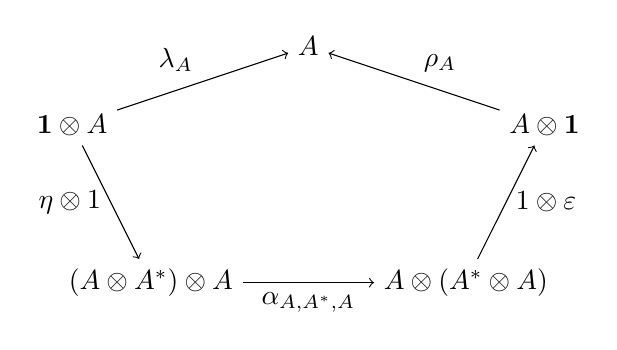
\begin{tikzpicture}
                \node (A) at (0, 0) {$A$};
                \node (1A) at (-3, -1) {$\mathbf{1}\otimes A$};
                \node (A1) at (3, -1) {$A\otimes\mathbf{1}$};
                \node (1AAA) at (-2, -3) {$(A\otimes A^*)\otimes A$};
                \node (AAA1) at (2, -3) {$A\otimes(A^*\otimes A)$};
                \draw[->] (1A) -- node[above left]{$\lambda_A$} (A);
                \draw[->] (A1) -- node[above right]{$\rho_A$} (A);
                \draw[->] (1A) -- node[left]{$\eta\otimes\mathbbm{1}$} (1AAA);
                \draw[->] (AAA1) -- node[right]{$\mathbbm{1}\otimes\varepsilon$} (A1);
                \draw[->] (1AAA) -- node[below]{$\alpha_{A, A^*, A}$} (AAA1);
            \end{tikzpicture}
            \caption{Dual object I.}
            \label{fig:dual_object1}
        \end{figure}
        \begin{figure}[ht!]
            \centering
            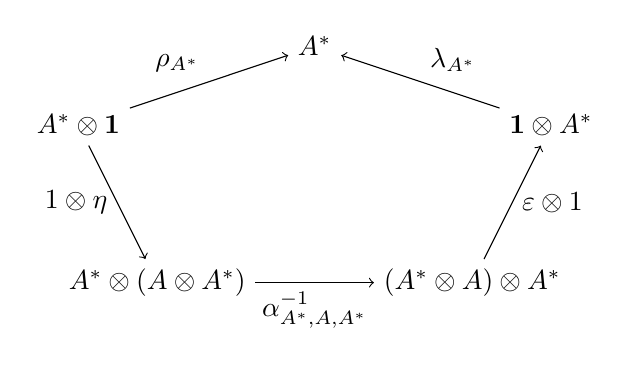
\begin{tikzpicture}
                \node (A) at (0, 0) {$A^*$};
                \node (A1) at (-3, -1) {$A^*\otimes\mathbf{1}$};
                \node (1A) at (3, -1) {$\mathbf{1}\otimes A^*$};
                \node (AAA1) at (-2, -3) {$A^*\otimes(A\otimes A^*)$};
                \node (1AAA) at (2, -3) {$(A^*\otimes A)\otimes A^*$};
                \draw[->] (A1) -- node[above left]{$\rho_{A^*}$} (A);
                \draw[->] (1A) -- node[above right]{$\lambda_{A^*}$} (A);
                \draw[->] (A1) -- node[left]{$\mathbbm{1}\otimes\eta$} (AAA1);
                \draw[->] (1AAA) -- node[right]{$\varepsilon\otimes\mathbbm{1}$} (1A);
                \draw[->] (AAA1) -- node[below]{$\alpha^{-1}_{A^*, A, A^*}$} (1AAA);
            \end{tikzpicture}
            \caption{Dual object II.}
            \label{fig:dual_object2}
        \end{figure}
    }

    \newdef{Rigid category\footnotemark}{\index{category!rigid}\index{category!autonomous}
        \footnotetext{Also called an \textbf{autonomous category}.}
        A monoidal category in which all duals exist. If only left (resp. right) duals exist then the category is said to be left (resp. right) rigid.
    }

    \begin{property}[Braided categories]\label{cat:braided_rigid}
        In general it is not true that left and right duals coincide, however in a braided monoidal category this is the case.
    \end{property}
    \newdef{Compact closed category}{\index{category!compact closed}
        A symmetric rigid category is also called a compact closed category.
    }

    \begin{example}[FinVect]\index{dual!space}\index{resolution!of the identity}
        Consider the category $\mathbf{FinVect}$ of finite-dimensional vector spaces (the ground field is assumed to be $\mathbb{R}$). The categorical dual of a vector space $V$ is the algebraic dual $V^*$. The unit morphism is given by the ''resolution of the identity'':
        \begin{gather}
            \eta: \mathbf{1}\rightarrow V\otimes V^*:1\mapsto\sum_{i=1}^{\dim(V)}e_i\otimes \phi^i
        \end{gather}
        where $\{e_i\}$ and $\{\phi^i\}$ are bases of $V$ and $V^*$ respectively.

        It should be noted that the category $\mathbf{Vect}$ of all vector spaces is not rigid. By property \ref{cat:braided_rigid} above, left and right duals coincide in any braided monoidal category (such as $\mathbf{Vect}$). However for infinite-dimensional vector spaces it is known that $A\cong(A^*)^*$ never holds and as such the rigidity cannot be extended to $\mathbf{Vect}$.
    \end{example}
    \begin{property}[Tannaka duality]\index{Tannaka duality}
        Consider the category $\mathcal{V}=\mathbf{FinVect}_K$, where the underlying ground field is now explicitly mentioned. Using coends one can reconstruct the base field from its modules, i.e. the objects in $\mathcal{V}$:\footnote{This result can be shown to hold for all compact closed categories $\mathcal{V}$. In this context it is known as \textbf{Tannaka reconstruction}.}
        \begin{gather}
            \int^{V\in\mathcal{V}}V^*\otimes V\cong K.
        \end{gather}
        A more general statement goes as follows:
        \begin{gather}
            \int^{V\in\mathcal{V}}\mathcal{V}(V, -)\otimes\text{id}_{\mathcal{V}}V\cong\text{id}_{\mathcal{V}}.
        \end{gather}
        The components $\eta_V:\mathcal{V}(V, V)\rightarrow K$ of the coend can be shown to coincide with the trace and such the trace obtains a universal property.
    \end{property}
    \remark{This property can also be generalized by replacing $\mathcal{V}$ by a category $\mathbf{Mod}_A$ for some finite-dimensional algebra $A$. The end and coend than give respectively the algebra $A$ and its dual $A^*$.}

    The trace on $\mathbf{FinVect}$ can be generalized as follows:
    \newdef{Trace}{\index{trace}
        Let $(\mathbf{C}, \otimes, \mathbf{1})$ be a rigid category and let $f\in\hom_{\mathbf{C}}(A, A^{**})$. The left (\textbf{categorical} or \textbf{quantum}) trace of $f$ is defined as the following morphism in End$_{\mathbf{C}}(\mathbf{1})$:
        \begin{gather}
            \text{tr}^L(f):=\varepsilon_{A^*}\circ(f\otimes\mathbbm{1})\circ\eta_A.
        \end{gather}
        If $f\in\hom_{\mathbf{C}}(A, ^{**}A)$ then the right trace is defined similarly:
        \begin{gather}
            \text{tr}^R(f):=\varepsilon_{^{**}A}\circ(\mathbbm{1}\otimes f)\circ\eta_{^*A}.
        \end{gather}
    }
    \begin{property}
        The following linear algebra-like properties hold for the categorical trace:
        \begin{itemize}
            \item $\text{tr}^L(f) = \text{tr}^R(f^*)$,
            \item $\text{tr}^L(f\otimes g) = \text{tr}^L(f)\text{tr}^L(g)$, and
            \item For additive categories: $\text{tr}^L(f\oplus g) = \text{tr}^L(f) + \text{tr}^L(g)$.
        \end{itemize}
        The second and third property can be stated analogously for the right trace.
    \end{property}

    \newdef{Pivotal category}{\index{pivotal structure}
        Let $\mathbf{C}$ be a rigid monoidal category. A pivotal structure on $\mathbf{C}$ is a monoidal natural isomorphism $a_A:A\cong A^{**}$.
    }

    \newdef{Dimension}{\index{dimension}
        Let $(\mathbf{C}, a)$ be a pivotal category and consider an object $V\in\ob{C}$. The dimension of $V$ is defined as follows:
        \begin{gather}
            \label{category:pivotal_dimension}
            \dim_a(V) := \text{tr}^L(a_V).
        \end{gather}
    }

    \newdef{Spherical category}{\index{spherical structure}
        Let $(\mathbf{C}, a)$ be a pivotal category. If the left and right traces (with respect to $a$) coincide in $\mathbf{C}$, i.e. $\dim_a(V) = \dim_a(V^*)$, then the pivotal structure is said to be spherical.
    }

    \newdef{Symmetric monoidal dagger category}{\index{category!dagger}
        A symmetric monoidal category $(\mathbf{C},\otimes,\mathbf{1})$ which also carries the structure of a dagger category \ref{cat:dagger_category} such that
        \begin{gather}
            (f\otimes g)^\dag = f^\dag\otimes g^\dag
        \end{gather}
        and such that the coherence and braiding morphisms are unitary.
    }
    \newdef{Dagger-compact category}{
        A symmetric monoidal dagger category which is also a compact closed category such that the following diagram commutes:
        \begin{gather*}
            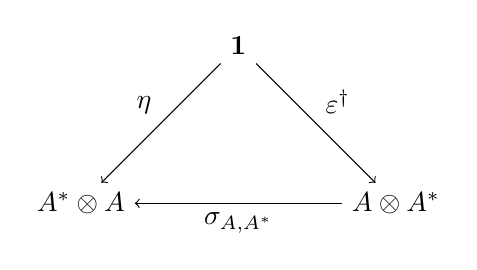
\begin{tikzpicture}
                \node (1) at (0, 0) {$\mathbf{1}$};
                \node (A*A) at (-2, -2) {$A^*\otimes A$};
                \node (AA*) at (2, -2) {$A\otimes A^*$};
                \draw[->] (1) -- node[above left]{$\eta$} (A*A);
                \draw[->] (1) -- node[above right]{$\varepsilon^\dagger$} (AA*);
                \draw[<-] (A*A) -- node[below]{$\sigma_{A,A^*}$} (AA*);
            \end{tikzpicture}
        \end{gather*}
    }

\section{Tensor and fusion categories}

    Some definitions might slightly differ from the ones in the main reference and some properties might be stated less generally. $k$ denotes an algebraically closed field (often this will be $\mathbb{C}$).

    \newdef{Tensor category}{\index{tensor!category}
        A monoidal category with the following properties:
        \begin{enumerate}
            \item it is rigid,
            \item it is Abelian,
            \item it is $k$-linear (and it is so in a way compatible with the Abelian structure),
            \item $\text{End}(\mathbf{1})\cong k$, and
            \item $-\otimes -$ is bilinear on morphisms.
        \end{enumerate}
        Some authors (such as \cite{etingof}) also add ''locally finite'' as a condition (see definition \ref{category:locally_finite}).
    }
    \remark{If $k$ is not algebraically closed one should exchange the last condition by the condition that $\mathbf{1}$ is a simple object. However, if $k$ is algebraically closed then these statements are equivalent.}

    \newdef{Pointed tensor category}{\index{pointed!tensor category}
        A tensor category is said to be pointed if all of its simple objects are (weakly) invertible.
    }

    \newdef{Fusion category}{\index{fusion!category}
        A semisimple finite tensor category.
    }

    \begin{property}
        Let $\mathbf{M}$ be a fusion category. There exists a natural isomorphism $X\cong X^{**}$.
    \end{property}

    \sremark{Although any fusion category admits a natural isomorphism between an object and its double dual, this morphism does not need to be monoidal. The fact that all fusion categories are pivotal was conjectured by \textit{Etingof, Ostrik} and \textit{Nikshych}. Currently the best one can do for a general fusion category is a monoidal natural transformation between the identity functor and the fourth dualization functor $X\cong X^{****}$.}

    \newdef{Categorical dimension}{\index{dimension}
        Consider a fusion category $\mathbf{M}$ and choose a natural isomorphism $a:\text{id}_{\mathbf{M}}\xrightarrow{\ \sim\ }\ast\ast$. For every simple object $X$ one can define a dimension function, sometimes called the \textbf{norm squared}, in the following way:
        \begin{gather}
            |X|^2 = \text{tr}(a_X)\text{tr}((a_X^{-1})^*).
        \end{gather}
        If $\mathbf{M}$ is pivotal then this becomes $|X|^2 = \dim_a(X)\dim_a(X^*)$. In particular, when $\mathbf{M}$ is spherical, this becomes $|X|^2 = \dim_a(X)^2$.

        The categorical dimension\footnote{Sometimes called the \textbf{M\"uger dimension}.} is then defined as follows:
        \begin{gather}
            \dim(\mathbf{M}) = \sum_{X\in\mathcal{O}(\mathbf{M})}|X|^2
        \end{gather}
        where $\mathcal{O}(\mathbf{M})$ denotes the set of isomorphism classes of simple objects.
    }
    \remark{It should be noted that the above quantities do not depend on the choice of isomorphism $a_X:X\cong X^{**}$ since all of them only differ by a scale factor.}
    \begin{property}
        For any fusion category $\mathbf{M}$ one has that $\dim(\mathbf{M})\neq 0$. In particular, if $k=\mathbb{C}$ then $\dim(\mathbf{M})\geq1$ (since the norm squared of any simple object is then also positive).
    \end{property}

    \newdef{$G$-graded fusion category}{\index{G!grading}
        A semisimple linear category $\mathbf{C}$ is said to have a \textbf{$G$-grading}, where $G$ is a finite group, if it can be decomposed as follows:
        \begin{gather}
            \mathbf{C}\cong\bigoplus_{g\in G}\mathbf{C}_g,
        \end{gather}
        where every $\mathbf{C}_g$ is again linear and semisimple. A fusion category $\mathbf{C}$ is said to be a ($G$-)graded fusion category if it admits a $G$-grading such that the tensor product functor maps $\mathbf{C}_g\times\mathbf{C}_h$ into $\mathbf{C}_{gh}$.
    }

    \begin{example}[$G$-graded vector spaces]\label{category:g_graded}
        Define the category $\mathbf{Vect}_G^\omega$ as having the same objects and morphisms as $\mathbf{Vect}_G$ (the category of $G$-graded vector spaces) but with the associator given by the the 3-cocycle $\omega\in H^3(G; k^\times)$.
    \end{example}
    \begin{property}
        Any pointed fusion category is equivalent to a category of the form $\mathbf{Vect}_G^\omega$ for some $G$ and $\omega\in H^3(G; k^\times)$.
    \end{property}

    \begin{theorem}[Tannaka duality]\index{Tannaka duality}
        The representation category of a weak Hopf algebra has the structure of a fusion category. Conversely, any fusion category can be obtained as the representation category of a weak Hopf algebra.
    \end{theorem}

\section{Ribbon and modular categories}

    \newdef{Ribbon structure}{
        Consider a braided monoidal category $(\mathbf{M}, \otimes, \mathbf{1})$ with braiding $\sigma$. A \textbf{twist} or \textbf{balancing} is a natural transformation $\theta$ such that the following equation is satisfied for all $X, Y\in\ob{M}$:
        \begin{gather}
            \theta_{X\otimes Y} = (\theta_X\otimes\theta_Y)\circ\sigma_{Y, X}\circ\sigma_{X, Y}.
        \end{gather}
        If in addition $\mathbf{M}$ is rigid and the twist satisfies $\theta_{X^*} = (\theta_X)^*$ for all $X\in\ob{M}$ then one speaks of a ribbon category.
    }

    \newdef{Drinfeld morphism}{
        Let $(\mathbf{M}, \otimes, \mathbf{1})$ be a rigid braided monoidal category with braiding $\sigma$. This structure admits a canonical natural isomorphism $X\cong X^{**}$ defined as follows:
        \begin{gather}
            X\xrightarrow{\mathbbm{1}_X\otimes\eta_{X^*}}X\otimes X^*\otimes X^{**}\xrightarrow{\sigma_{X, X^*}\otimes\mathbbm{1}_{X^{**}}}X^*\otimes X\otimes X^{**}\xrightarrow{\varepsilon_X\otimes\mathbbm{1}_{X^{**}}}X^{**}.
        \end{gather}
    }
    \begin{property}
        Let $\mathbf{M}$ be a braided monoidal category. Consider the canonical natural isomorphism $u_X:X\cong X^{**}$ defined above. Any natural isomorphism $\psi_X:X\cong X^{**}$ can be written as $u_X\theta_X$ where $\theta\in\text{Aut}(\mathbbm{1}_{\mathbf{M}})$. It is not hard to see that this natural isomorphism is monoidal (hence pivotal) exactly when $\theta$ is a twist. If $\mathbf{M}$ is a fusion category then the pivotal structure is spherical if and only if $\theta$ gives a ribbon structure.
    \end{property}

    \newdef{Premodular category}{
        A ribbon fusion category. Equivalently, a spherical braided fusion category.
    }
    \newdef{$S$-matrix}{\index{S-matrix}
        Given a premodular category $\mathbf{M}$ (with braiding $\sigma$) one defines the $S$-matrix as follows:
        \begin{gather}
            S_{X, Y} := \text{tr}(\sigma_{Y, X}\circ\sigma_{X, Y})
        \end{gather}
        where $X, Y$ are (isomorphism classes of) simple objects.

        Since in a premodular category there are only finitely many isomorphism classes of simple objects (denote this number by $\mathcal{I}$), one can see that $S$ is a $\mathcal{I}\times\mathcal{I}$-matrix.
    }

    \newdef{Modular category\footnotemark}{\index{modular!category}
        \footnotetext{A modular (tensor) category is often abbreviated as \textbf{MTC}.}
        A premodular category for which the $S$-matrix is invertible.
    }

    \begin{property}
        Let $\mathbf{M}$ be a modular category with $S$-matrix $S$. If $E$ denotes the matrix such that $E_{X,Y}$ is 1 if $X=Y^*$ and 0 otherwise, the following relation with the categorical dimension of $\mathbf{M}$ is obtained:
        \begin{gather}
            S^2 = \dim(\mathbf{M})E.
        \end{gather}
    \end{property}

    \begin{formula}[Verlinde]
        Consider a modular category $\mathbf{M}$ with $S$-matrix $S$. Let $\mathcal{O}(\mathbf{M})$ denote the set of isomorphism classes of simple objects and let $\dim(R)$ denote the dimension of an object $R$ defined using the spherical structure on $\mathbf{M}$. Using the formula
        \begin{gather}
            S_{X, Y}S_{X, Z} = \dim(X)\sum_{W\in\mathcal{O}(\mathbf{M})}N_{Y, Z}^WS_{X, W}
        \end{gather}
        for all $X, Y, Z\in\mathcal{O}(\mathbf{M})$ one obtains the following important relation:
        \begin{gather}
            \sum_{W\in\mathcal{O}(\mathbf{M})}\frac{S_{W, Y}S_{W, Z}S_{W, X^*}}{\dim(W)} = \dim(\mathbf{M})N_{Y, Z}^X.
        \end{gather}
        This property implies that the $S$-matrix of a modular category determines the fusion coefficients of the underlying fusion category.
    \end{formula}

\section{Module categories}
\subsection{Over a monoidal category}

    By categorifying the definition of a module over a ring one obtains the notion of a module category:
    \newdef{Module category}{\index{module!category}
        Let $\mathbf{M}$ be a monoidal category. A left $\mathbf{M}$-module (category) is a linear category $\mathbf{C}$ equipped with a bilinear functor $\func{\triangleright}{M\times C}{C}$  together with natural isomorphisms that categorify the associativity and unit conditions of modules (these are also required to be compatible with the associator and unitors of $\mathbf{M}$).
    }
    \remark{Similar to how a $G$-set can be defined as a functor $\mathbf{B}G\rightarrow\mathbf{Set}$, one can define a module category as a 2-functor $\mathbf{BM}\rightarrow\mathbf{Cat}$.}

    Analogous to definition \ref{category:internal_hom} one can also define internal homs for module categories:
    \newdef{Internal hom}{\index{internal!hom}
        Consider a left $\mathbf{M}$-module $\mathbf{C}$. Given two objects $c,c'\in\ob{C}$ one defines their internal hom (if it exists) as the object $\underline{\hom}(c, c')\in\ob{M}$ satisfying the following condition
        \begin{gather}
            \mathbf{C}(m\triangleright c, c')\cong\mathbf{M}(m, \underline{\hom}(c, c'))
        \end{gather}
        for all $m\in\ob{M}$.
    }
    \begin{property}
        It should be noted that for the case $\mathbf{C}\equiv\mathbf{M}$ (where the action is given by the tensor product in $\mathbf{M}$) one obtains Definition \ref{category:internal_hom} as a particular case.
    \end{property}

\section{Higher vector spaces}
\subsection{Kapranov-Voevodksy 2-vector spaces}

    The guiding principle for this definition of 2-vector spaces will be the generalization of certain observations from studying the category $\mathbf{Vect}$ of ordinary vector spaces. Linear maps between vector spaces can (at least for finite dimensions) be represented as matrices with coefficient in the ground field $k$. Coincidentally this ground field is also the tensor unit in $\mathbf{Vect}$. At the same time all finite-dimensional vector spaces are isomorphic to spaces of the form $k^n$ (where $n$ is given by the dimension of the vector space).

    \newdef{2-vector space}{\index{2-vector space!Kapranov-Voevodsky}
        To define 2-vector spaces, Kapranov and Voevodsky lifted these observations to 1 dimension higher by replacing the ground field $\mathbb{C}$ by the category $\mathbf{Vect}$. To wit $\mathbf{2Vect}$ is defined as the 2-category consisting of the following data:
        \begin{enumerate}
            \item objects: Finite products of the form $\mathbf{Vect}^n$;
            \item 1-morphisms: \textbf{2-matrices}, i.e. collections $||A_{ij}||$ of finite-dimensional vector spaces; and
            \item 2-morphisms: collections $(a_{ij})$ of linear maps (between finite-dimensional vector spaces).
        \end{enumerate}
        The multiplication (composition) of 1-morphisms is defined in analogy to the multiplication of ordinary matrices, but where the usual sum and product are replaced by the direct sum and tensor product.
    }

    A seemingly more formal definition uses the concepts of \textit{ring} and \textit{module categories}:
    \begin{adefinition}
        A 2-vector space is a lax module category over the ring category $\mathbf{Vect}$ which is module-equivalent to $\mathbf{Vect}^n$ for some $n\in\mathbb{N}$. The 2-category $\mathbf{2Vect}$ is then defined as the 2-category with objects these 2-vector spaces, as 1-morphisms the associated $\mathbf{Vect}$-module functors and as 2-morphisms the module natural transformations.
    \end{adefinition}

\subsection{Baez-Crans 2-vector spaces}\label{section:baez_crans}

    \newdef{2-vector space}{\index{2-vector space!Baez-Crans}\index{linear!functor}
        A category internal to $\mathbf{Vect}$.\footnote{For the definition of internal categories see \ref{cat:internal_category}.} The relevant notion of morphism is that of a \textbf{linear functor}, i.e. a functor internal to $\mathbf{Vect}$.
    }
    \remark{The above definition should not be confused with that of categories and functors enriched over $\mathbf{Vect}$.}

    \begin{example}[Ground field]
        The ground field $k$ can be categorified to a 2-vector spaces by taking $K_0=K_1:=k$ and $s=t=e:=\mathbbm{1}_k$. This object serves a unit for the tensor product on $\mathbf{2Vect}$.
    \end{example}

    \begin{property}[Chain complexes]
        There exists an equivalence between the (2-)categories of 2-vector spaces and 2-term chain complexes.
        \begin{proof}[Sketch of construction]
            Given a 2-vector space $(V_0, V_1)$, one can build a chain complex $C_\bullet$ as follows:
            \begin{itemize}
                \item $C_0 := V_0$,
                \item $C_1 := \ker(s)$, and
                \item $d := t|_{C_1}$
            \end{itemize}
            where $s,t$ are the source morphism and target morphisms.
        \end{proof}
    \end{property}
    \remark{The equivalence (on the level of ordinary categories) is an instance of the Dold-Kan correspondence \ref{sheaf:dold_kan}.}

    \newdef{Arrow part}{\index{arrow}
        Consider a 2-vector space $V=(V_0,V_1)$. For any morphism $f\in V_1$ one defines the arrow part as follows:
        \begin{gather}
            \vec{f} := f - e(s(f))
        \end{gather}
        where $e, s$ are the identity and source morphisms in $V$. Any map can thus be recovered from its arrow part and its source. This allows us to identify a map $f\in V_1$ with the pair $\big(s(f),\vec{f}\ \big)$. Using arrow parts one can rewrite the composition law of morphisms in an intuitive way:
        \begin{gather}
            g\circ f = \big(s(f), \vec{f} + \vec{g}\,\big).
        \end{gather}
    }

    \newdef{Antisymmetric natural morphism}{\index{antisymmetry}
        A natural morphism between $n$-linear functors in \textbf{2-Vect} is said to be \textbf{completely antisymmetric} if its arrow part is completely antisymmetric.
    }

\section{Higher Lie theory}
\subsection{Lie superalgebras}

    \newdef{Internal Lie algebra}{\index{Lie!algebra}
        Let $(\textbf{C}, \otimes, \mathbf{1})$ be a linear symmetric monoidal category with braiding $\sigma$. A Lie algebra internal to \textbf{C} is an object $A\in\ob{C}$ and a morphism \[[\cdot, \cdot]:A\otimes A\rightarrow A\] satisyfing the following conditions:
        \begin{enumerate}
            \item \textbf{Antisymmetry}: $[\cdot, \cdot] + [\cdot, \cdot]\circ\sigma_{A, A} = 0$, and
            \item \textbf{Jacobi identity}: $[\cdot, [\cdot, \cdot]] + [\cdot, [\cdot, \cdot]]\circ\tau + [\cdot, [\cdot, \cdot]]\circ\tau^2= 0$,
        \end{enumerate}
        where $\tau = (\mathbbm{1}\otimes\sigma_{A, A})\circ(\sigma_{A, A}\otimes\mathbbm{1})$ denotes cyclic permutation.
    }
    \begin{example}[Lie superalgebra]\label{hda:lie_superalgebra}
        When using the braiding $\sigma(a\otimes b) = (-1)^{\deg(a)\deg(b)}b\otimes a$ in \textbf{sVect}, a Lie superalgebra (also called a super Lie algebra) is obtained.
    \end{example}
    \begin{example}[dg-Lie algebras]
        Lie algebras internal to $\mathbf{Ch}_\bullet(\mathbf{Vect})$ or its generalization to graded vector spaces. Sometimes these are also called strict $L_\infty$-algebras (see further below).
    \end{example}

    \newdef{Semistrict Lie 2-algebra}{\index{Lie!bracket}\index{Jacobiator}\index{Zamolodchikov tetrahedron equation}
        A (Baez-Crans) 2-vector space $V\equiv(V_0,V_1)$ equipped with the following morphisms:
        \begin{enumerate}
            \item an antisymmetric bilinear functor $[\cdot,\cdot]:V\times V\rightarrow V$ (the \textbf{bracket}), and
            \item a completely antisymmetric trilinear natural isomorphism
                \begin{gather}
                    J_{x,y,z}: [[x,y],z]\rightarrow[x,[y,z]]+[[x,z],y],
                \end{gather}
                called the \textbf{Jacobiator}.
        \end{enumerate}
        These structures are required to satisfy the \textit{Jacobiator identity} (which is just the \textit{Zamolodchikov tetrahedron equation}). If the Jacobiator is trivial, a \textbf{strict} Lie 2-algebra is obtained. By further relaxing the antisymmetry, one can obtain the fully weak version of Lie 2-algebras (see for example the work by \textit{Roytenberg}).
    }

    From the previous section it follows that one can define (weak) Lie 2-algebras as 2-term chain complexes equipped with a coherent Lie bracket:
    \newadef{Lie 2-algebra}{\index{Lie!2-algebra}\index{alternator}\index{hemistrict}\label{hda:2-algebra}
        Consider a 2-term chain complex in the category $\mathbf{FinVect}$:
        \begin{gather}
            0\longrightarrow L_1\longrightarrow L_0\longrightarrow 0.
        \end{gather}
        This complex $L$ is called a Lie 2-algebra if it comes equipped with the following structures:
        \begin{enumerate}
            \item a chain map $[\cdot,\cdot]:L\otimes L\rightarrow L$ called the \textbf{bracket},
            \item a chain homotopy $S:[\cdot,\cdot]\Rightarrow-[\cdot,\cdot]\circ\sigma$ called the \textbf{alternator}, and
            \item a chain homotopy
                \begin{gather}
                    J:[\cdot,[\cdot,\cdot]]\Rightarrow[[\cdot,\cdot],\cdot] + [\cdot,[\cdot,\cdot]]\circ(\sigma\otimes\mathbbm{1}),
                \end{gather}
                called the \textbf{Jacobiator}.
        \end{enumerate}
        These chain homotopies are again required to satisfy higher coherence relations. From the previous definition it follows that the vanishing of the alternator implies that $L$ is semistrict. Analogously, one calls a Lie 2-algebra for which the Jacobiator vanishes \textbf{hemistrict}. Note that this definition of weak Lie 2-algebras, when translated to the 2-vector space setting, would imply that the alternator and Jacobiator are merely natural transformations (and not isomorphisms)!
    }

\subsection{\texorpdfstring{Lie $n$-algebras}{Lie n-algebras}}\label{section:higher_lie_structures}

    \newdef{Semistrict Lie $\omega$-algebra}{
        By replacing internal categories by internal \textit{$\omega$-categories} and by relaxing the Jacobiator identity up to coherent homotopy, i.e. up to a completely antisymmetric quadrilinear modification which in turn satisfies an identity up to higher multilinear transfors, one obtains the definition of $L_\infty$-algebras. Similar to $A_\infty$-algebras, these too can be obtained as algebras over a suitable operad (however, in this case the operad is ``slightly'' more complex: the cofibrant replacement of the \textit{Lie operad}).

        It can be shown that these structures are equivalent to the $L_\infty$-algebras of \textit{Stasheff} defined below.
    }

    \newdef{$L_\infty$-algebra\footnotemark}{\index{$L_\infty$-algebra}\index{signature}\label{lie:l_infinity}
        \footnotetext{Also called a \textbf{strong(ly) homotopy Lie algebra} (abbreviated to \textbf{sh Lie algebra}).}
        A graded vector space $V$ equipped with a collection of morphisms $l_n:V^{\otimes n}\rightarrow V, n\in\mathbb{N}_0$ of degree $n-2$ subject to the relations
        \begin{gather}
            l_n(v_{\sigma(1)}\ldots v_{\sigma(n)}) = \chi(\sigma;v_1,\ldots,v_n)l_n(v_1\ldots v_n)
        \end{gather}
        and
        \begin{gather}
            \sum_{\substack{i+j=n+1\\\sigma\in\text{Unshuff}(i,j-1)}}(-1)^{i(j-1)}\chi(\sigma;v_1,\ldots,v_n)l_i\big(l_j(v_{\sigma(1)}\cdots v_{\sigma(j)})v_{\sigma(j+1)}\cdots v_{\sigma(n)}\big)=0,
        \end{gather}
        where Unshuff denotes the collection of unshuffles \ref{group:shuffle}.

        The $l_1$ map turns the $L_\infty$-algebra into a chain complex. The $l_2$ map is a generalized Lie bracket since it is (graded-)antisymmetric. Higher $l_n$'s can be identified with the Jacobiator and its generalizations. In the next section a bottom-up approach will be given.
    }
    \begin{remark}
        The definition can be rephrased in terms of graded maps $\hat{l}_n:\text{Alt}^\bullet V\rightarrow V$.
    \end{remark}
    \begin{remark}[Curvature]\index{curvature}
        The above definition can be generalized by including a nullary bracket $l_0$. Such $L_\infty$-algebras are often said to be \textbf{curved}. The reason for this is that the coherence condition for $l_0$ says that
        \begin{gather}
            l_1\circ l_1 = l_2(l_0,-).
        \end{gather}
        This terminology stems from the situation where $l_1$ is identified with the exterior covariant derivative on an associated vector bundle (Formula \ref{diff:curvature_associated_bundles}).
    \end{remark}

    \begin{example}[Lie algebra]\index{Lie!algebra}
        It can easily be checked that the $L_\infty$-algebra with $V$ concentrated in degree 1 is equivalent to the structure of an ordinary Lie algebra. Similarly one obtains the notion of a Lie $n$-algebra by truncating an $L_\infty$-algebra at degree $n$.
    \end{example}

    \begin{property}
        2-term $L_\infty$-algebras, or equivalently semistrict Lie $2$-algebras, are in correspondence with isomorphism classes of tuples $(\mathfrak{g},V,\rho,l_3)$ where $\mathfrak{g}$ is a Lie algebra, $(V,\rho)$ is Lie algebra representation of $\mathfrak{g}$ and $l_3$ is a $V$-valued Lie algebra 3-cocycle (Section \ref{section:lie_algebra_cohomology}).

        \begin{proof}[Sketch of construction]
            Using the representation $\rho$, one can extend the Lie bracket from $\mathfrak{g}$ to the complex $0\rightarrow V\rightarrow\mathfrak{g}\rightarrow0$ through the formulas $[g,v]:=\rho(g)v$ and $[v,g] := -[g,v]$. The cocycle condition for $l_3$ gives rise to the Jacobiator.
        \end{proof}
    \end{property}
    \begin{example}\label{hda:gk_lie_2_algebra}
        If one chooses a finite-dimensional Lie algebra $\mathfrak{g}$ with the trivial representation on $\mathbb{R}$ (or, more generally, the underlying field of $\mathfrak{g}$), one obtains
        \begin{gather}
            H^3(\mathfrak{g};\mathbb{R})\cong\mathbb{R}.
        \end{gather}
        The different classes can be represented by scalar multiples of the Killing cocycle from Example \ref{lie:killing_transgression}. For every such scalar $\lambda\in\mathbb{R}$, one denotes the resulting Lie 2-algebra by $\mathfrak{g}_\lambda$.
    \end{example}

    Lie algebras and $L_\infty$-algebras can also be dually characterized in terms of their Chevalley-Eilenberg algebra \ref{lie:chevalley_eilenberg_algebra}:
    \newadef{Lie algebra}{\index{Lie!algebra}
        Consider a finite-dimensional Lie algebra $\mathfrak{g}$. The transpose/dual of the Lie bracket $[\cdot,\cdot]:\mathfrak{g}\wedge\mathfrak{g}\rightarrow\mathfrak{g}$ is a morphism $\delta:\mathfrak{g}^*\rightarrow\mathfrak{g}^*\wedge\mathfrak{g}^*$:
        \begin{gather}
            \delta\omega(g,h) := \omega([g,h]).
        \end{gather}
        In fact, it is not hard to see that this is exactly the Chevalley-Eilenberg differential of $\text{CE}(\mathfrak{g})$. Conversely, given a semifree DGCA $(\Lambda^\bullet V^*,d)$, for some finite-dimensional vector space $V$, one obtains a finite-dimensional Lie algebra by restricting the differential to $V^*$ and taking the transpose. In fact, the nilpotency condition $d^2=0$ is equivalent to the Jacobi identity.
    }

    More generally, by passing to graded vector spaces of finite type concentrated in positive degree, one can characterize $L_\infty$-algebras as semifree DGCAs:
    \newadef{$L_\infty$-algebra}{\index{$L_\infty$-algebra}\label{hda:l_infinity_bis}
        The (graded) Leibniz rule implies that the differential $\delta$ is completely defined by its restriction to the generators $V^*\leq\Alt^\bullet V^*$. The differential can be decomposed as follows:
        \begin{gather}
            \delta t^a := -\sum_{k=1}^\infty\frac{1}{k!}[t_{a_1},\ldots,t_{a_k}]^a_k\, t^{a_1}\wedge\cdots\wedge t^{a_k},
        \end{gather}
        where the basis $t^a$ of $V^*$ is dual to the basis $t_a$ of $V$. Because $\delta$ is of degree $1$, the coefficients $[\cdots]_k^a$ define a multilinear operator $[\cdots]_k:\Alt^kV\rightarrow V$ of degree $n-1$ (some sources rephrase these brackets as morphism from the symmetric algebra $\Sym^\bullet V$, in which case their degree is just -1, cf. d\'ecalage \ref{hda:decalage}).

        The nilpotency condition $\delta^2=0$ implies a list of (quadratic) relations on the brackets $[\cdots]_k$ (with $d:=[\cdot]_1$):
        \begin{align*}
            d^2&=0\\
            d[\cdot,\cdot]_2 &= [d\cdot,\cdot]_2+[\cdot,d\cdot]_2\\
            [[v_1,v_2],v_3]_2+\text{cyc. perm.} &= d[v_1,v_2,v_3]_3-[dv_1,v_2,v_3]_3-[v_1,dv_2,v_3]_3-[v_1,v_2,dv_3]_3\\
            &\ \ \vdots
        \end{align*}
        These relations can be interpreted as follows:
        \begin{itemize}
            \item $d$ is a differential.
            \item $d$ acts as a derivation with respect to the binary bracket.
            \item The Jacobi identity holds up to a chain homotopy (given by the ternary bracket).
            \item The higher relations are similar to the chain homotopy for the Jacobi identity.
        \end{itemize}
        When written out it in full detail it can be checked that this is exactly the definition of an $L_\infty$-algebra.
    }

    \newdef{Maurer-Cartan element}{\index{Maurer-Cartan!equation}
        An element $a$ of an $L_\infty$-algebra $V$ that satisfies the equation
        \begin{gather}
            \sum_{k=0}^\infty\frac{1}{k!}[a,\ldots,a]_k=0.
        \end{gather}
        For dg-Lie algebras this reduces to the ordinary Maurer-Cartan equation \ref{diff:mc_equation}:
        \begin{gather}
            da + \frac{1}{2}[a,a] = 0.
        \end{gather}
        This is no coincidence since the complex $\Omega^\bullet(M)\otimes\mathfrak{g}$ of Lie algebra-valued differential forms on a smooth manifold $M$ carries a canonical dg-Lie algebra structure.
    }

\section{\texorpdfstring{Monoidal $n$-categories}{Monoidal n-categories}}\label{section:monoidal_n_cat}

    \newdef{Monoidal $n$-category}{\index{monoidal!$n$-category}
        In general one can define a monoidal $n$-category as a one-object $(n+1)$-category, similar to how monoidal categories give one-object bicategories by delooping (see \ref{cat:monoidal_or_2}).
    }
    For the explicit definitions of monoidal bi- and tricategories, see the papers \cite{monbicat} and \cite{montricat} respectively.

    If one would put multiple compatible monoidal products on an $n$-category then by some kind of Eckmann-Hilton argument all of these structures will be equivalent to a ''commutative'' monoidal structure. By varying the number of compatible structures the ''commutativity'' can be increased. This gives rise to the following definition which is stated in different terms (based on the \textit{delooping hypothesis}):
    \newdef{$k$-tuply monoidal $n$-categories}{
        A pointed $(n+k)$-category (strict or weak) in which all parallel $j$-arrows for $j<k$ are equivalent. These categories form an $(n+k+1)$-category $\boldsymbol{k}\mathbf{Mon}\boldsymbol{n}\mathbf{Cat}$.
    }

    \begin{example}
        For small values of $k$ and $n$ the resulting structures coincide with some well-known constructions:
        \begin{itemize}
            \item $n=0$:
                \begin{itemize}
                    \item $k=0$: pointed set,
                    \item $k=1$: monoid, and
                    \item $k\geq2$: Abelian monoid.
                \end{itemize}
            \item $n=1$:
                \begin{itemize}
                    \item $k=0$: pointed\footnote{As in category with a specified element not as in category with a zero object (definition \ref{category:pointed_category}).} category,
                    \item $k=1$: monoidal category,
                    \item $k=2$: braided monoidal category, and
                    \item $k\geq3$: symmetric monoidal category.
                \end{itemize}
        \end{itemize}
    \end{example}
    The stabilization occurring for higher values of $k$ is the content of the following ''hypothesis''\footnote{For certain definitions of higher categories this has been proven in full generality.} (by \textit{Baez} \& \textit{Dolan}):
    \begin{theorem}[Stabilization hypothesis]\index{stabilization hypothesis}
        For values $k\geq n+2$ the structure of a $k$-tuply monoidal $n$-category becomes maximally symmetric. Formally this means that the inclusion \emph{$\boldsymbol{k}\mathbf{Mon}\boldsymbol{n}\mathbf{Cat}\hookrightarrow\boldsymbol{(n+2)}\mathbf{Mon}\boldsymbol{n}\mathbf{Cat}$} is an equivalence.
    \end{theorem}

\subsection[Relation to group cohomology]{Relation with group cohomology\footnotemark}\footnotetext{See definition \ref{group:cohomology} or section \ref{section:group_cohomology} for more information on group cohomology.}\label{section:hda_group_cohomology}

    Consider a finite group $G$. As a first step, construct the group algebra $\mathbb{C}[G]$. As a monoid one can consider this object as a $G$-graded monoidal 0-category. The ordinary multiplication $g\ast h=gh$ can be twisted to obtain a monoid $\mathbb{C}[G]^\omega$ with multiplication
    \begin{gather}
        g\ast h := e^{i\omega(g, h)}gh.
    \end{gather}
    If associativity is still required to hold on the nose, one is led to the property that $\omega$ is in fact a group 2-cocycle. The equivalence classes of such twisted group algebras are then in correspondence with the second cohomology class $H^2(G; \text{U}(1))$.

    Before really going to higher category theory, one should first reflect on the different structures in the previous paragraph. Since the monoid is regarded as a monoidal category (call it $M$ for convenience), one has a bifunctor $\mu:M\otimes M\rightarrow M$ (given by the twisted multiplication) that differs from the ordinary group multiplication by a phase. This phase can be viewed categorically as a natural isomorphism between the ''tensor products'' in $\mathbb{C}[G]$ and $M$. At the same time, all the higher coherence conditions\footnote{These can be parametrized by the \textit{Stasheff polytopes/associahedra}.\index{associahedron}} (associativity, ...) are required to hold identically.

    Now, drop the restriction on the product and take this to be a more general monoidal product bifunctor. To this end replace the monoid $\mathbb{C}[G]$ by the $G$-graded monoidal category $\mathbf{Vect}_G$ and relax the associativity constraint up to a natural isomorphism $\alpha$. When restricted to the simple objects of $\mathbf{Vect}_G$ this is given by a phase factor $e^{i\omega(g,h,k)}$. The pentagon condition for monoidal categories then implies that the function $\omega$ is a group 3-cocycle. In analogy with the case of monoids above the equivalence classes of (twisted) monoidal structures on $\mathbf{Vect}_G$ is in correspondence with the third cohomology group $H^3(G; \text{U}(1))$.

    To go yet another step higher, move up a level in the chain of coherence conditions and relax the associativity constraint even more (for ``simplicity'' the one-object $n$-category point of view is adopted here). Instead of a natural isomorphism it only has to be an adjoint equivalence and at the same time the pentagon condition is replaced by an invertible modification (3-morphism). The coherence condition on this \textbf{pentagonator}\index{pentagonator} then implies a classification of (twisted) monoidal bicategories, equivalent to $\mathbf{2Vect}_G^\omega$, by the fourth group cohomology $H^4(G; \text{U}(1))$.

    In a completely analogous way one can define more and more general structures. E.g. for monoidal tricategories one can translate the $K_6$ associahedron into an equation for an invertible perturbation (4-morphism) which by the $G$-graded structure is equivalent to a group 5-cocycle.

    \remark{This section is strongly related to the twisting procedure in $n$-dimensional Dijkgraaf-Witten theories.}

\part{Differential Geometry}\label{part:diffgeom}
\chapter{Curves and Surfaces}\label{chapter:curves_surfaces}
\section{Curves}

	\newdef{Regular curve}{\index{regular!curve}
		Let $\vector{c}(t):I\rightarrow\mathbb{R}^n$ be a curve defined on an interval $I$. $\vector{c}(t)$ is said to be regular\footnote{See also property \ref{manifolds:regular_point}.} if $\deriv{\vector{c}}{t}(t) \neq \vector{0}$ for all $t\in I$.
	}

	\newdef{Geometric property}{A geometric property is a property that is invariant under:
    		\begin{enumerate}
			\item parameter transformations
        		\item orientation-preserving (orthonormal) basis transformations
		\end{enumerate}
	}

	\begin{property}
		Let $\vector{c}(t), \vector{d}(t)$ be two curves with the same image. The following relation holds for all $t$:
	        \begin{gather}
			\vector{c}(t)\text{ regular}\iff\vector{d}(t)\text{ regular}.
		\end{gather}
	\end{property}

\subsection{Arc length}

    	\newdef{Natural parameter}{\index{natural!parameter}\label{diff:natural_parameter}
        	Let $\vector{c}(t)$ be a curve. The parameter $t$ is said to be a natural parameter if
	        \begin{gather}
	            	\left|\left|\deriv{\vector{c}}{t}\right|\right|\equiv1.
		\end{gather}
	}

        \begin{formula}[Arc length]\index{arc!length}\label{diff:arc_length_integral}
		The following function $\phi(t)$ is a bijective map and a natural parameter for the curve $\vector{c}$:
	        \begin{gather}
        	        \phi(t) = \int_{t_0}^t||\dot{\vector{c}}(t)||dt.
		\end{gather}
	\end{formula}
        \sremark{The arc length as defined above is often denoted by the letter $s$.}

        \begin{property}
		Let $\vector{c}(t)$ be a curve and let $u$ be an alternative parameter of $\vector{c}(t)$. It is a natural parameter if and only if there exists a constant $\alpha$ such that:\[u = \pm s + \alpha\] where $s$ is the integral as defined in equation \ref{diff:arc_length_integral}.
	\end{property}
        \begin{remark*}
		This property implies there does not exist a unique natural parameter or arc length for any curve.
	\end{remark*}

\subsection{Frenet-Serret frame}

    	\newdef{Tangent vector}{\index{tangent!vector}\label{diff:tangent_vector}
    		Let $\vector{c}(s)$ be a curve parametrized by arc length. The tangent vector (field) $\vector{t}(s)$ is defined as follows:
        	\begin{gather}
			\vector{t}(s) = \vector{c}\,'(s).
		\end{gather}
        }
        \begin{property}\label{diff:unit_tangent_vector}
		From the definition of the natural parametrization \ref{diff:natural_parameter} and the previous definition it follows that the tangent vector is automatically a unit vector.
	\end{property}

        \newdef{Principal normal vector}{\index{normal!vector}\label{diff:principal_normal_vector}
	        Let $\vector{c}(s)$ be a curve parametrized by arc length. The principal normal vector (field) is defined as follows:
        	\begin{gather}
			\vector{n}(s) = \stylefrac{\vector{t}\,'(s)}{||\vector{t}\,'(s)||}.
		\end{gather}
        }
        \begin{property}
		From property \ref{diff:unit_tangent_vector} and the definition of the principal normal vector it follows that the tangent vector and principal normal vector are always orthogonal.
	\end{property}

        \newdef{Binormal vector}{\label{diff:binormal_vector}
	        Let $\vector{c}(s)$ be a curve parametrized by arc length. The binormal vector (field) is defined as follows:
        	\begin{gather}
			\vector{b}(s) = \vector{t}(s)\times\vector{n}(s).
		\end{gather}
        }

        \newdef{Frenet-Serret frame}{\index{Frenet-Serret}\label{diff:frenet_serret_frame}
	        As the vectors $\vector{t}(s), \vector{n}(s)$ and $\vector{b}(s)$ are mutually orthonormal and linearly independent, we can use them to construct an oriented orthonormal basis. The ordered basis $\Big\{\vector{t}(s),\vector{n}(s), \vector{b}(s)\Big\}$ is called the Frenet-Serret frame.
	}
        \sremark{This basis does not have to be the same for every value of the parameter $s$.}

        \newdef{Curvature}{\index{curvature}\label{diff:curvature}
	        Let $\vector{c}(s)$ be a curve parametrized by arc length. The curvature of $\vector{c}(s)$ is defined as follows:
        	\begin{gather}
			\stylefrac{1}{\rho(s)} = ||\vector{t}\,'(s)||.
		\end{gather}
        }
        \newdef{Torsion}{\index{torsion}\label{diff:torsion}
        	Let $\vector{c}(s)$ be a curve parametrized by arc length. The torsion of $\vector{c}(s)$ is defined as follows:
        	\begin{gather}
			\tau(s) = \rho(s)^2(\vector{t}\ \ \vector{t}\,'\ \ \vector{t}\,'')
		\end{gather}
		where $(a b c)$ denotes the \textit{triple product} $a\cdot(b\times c)$.
        }

        \newformula{Frenet formulas}{\index{Frenet formulas}\label{diff:frenet_formulas}
        	The derivatives of the tangent, principal normal and binormal vector fields can be written as a linear combination of the those vectors themselves:
        	\begin{gather}
			\left\{
                	\begin{array}{ccccc}
				\vector{t}\,'(s) &=&& \stylefrac{1}{\rho(s)}\vector{n}(s)&\\
        	                \vector{n}\,'(s) &=& -\stylefrac{1}{\rho(s)}\vector{t}(s) &+& \tau(s)\vector{b}(s)\\
        	                \vector{b}\,'(s) &=& &-\tau(s)\vector{n}(s)&
			\end{array}
        	        \right.
		\end{gather}
        }

        \begin{theorem}[Fundamental theorem for curves]\index{fundamental theorem!for curves}\label{diff:theorem:fundamental_theorem_of_curves}
	        Let $k(s), w(s): U \rightarrow \mathbb{R}$ be two $\mathcal{C}^1$-functions with $k(s) \geq 0, \forall s\in U$. There exists an interval $]-\varepsilon, \varepsilon[\ \subset U$ and a curve $\vector{c}(s) :\ ]-\varepsilon, \varepsilon[\ \rightarrow \mathbb{R}^3$ with natural parameter $s$ such that $\vector{c}(s)$ has $k(s)$ as its curvature and $w(s)$ as its torsion.
	\end{theorem}

\section{Surfaces}

	\begin{notation}
	    	Let $\vector{\sigma}$ be the parametrization of a surface\footnote{The symbol $\vector{\sigma}$ denotes the surface as a vector field while $\Sigma$ denotes the geometric image of $\vector{\sigma}$.}. The derivative of $\vector{\sigma}$ with respect to the coordinate $q^i$ is written as follows:
	    	\begin{gather}
	    		\label{diff:derivative_of_surface}
			\pderiv{\vector{\sigma}}{q^i} = \vector{\sigma}_i.
		\end{gather}
	\end{notation}

    	\newdef{Tangent plane}{\index{tangent!plane}
        	Let $P(q_0^1,q_0^2)$ be a point on the surface $\Sigma$. The tangent space $T_P\Sigma$ to $\Sigma$ in $P$ is defined as follows:
	        \begin{gather}
			\label{diff:tangent_space}
        	        \forall \vector{r}\in T_P\Sigma : \left[\vector{r} - \vector{\sigma}(q_0^1,q_0^2)\right]\cdot\left[\vector{\sigma}_1(q_0^1,q_0^2)\times\vector{\sigma}_2(q_0^1,q_0^2)\right] = 0.
		\end{gather}
        }

        \newdef{Normal vector}{\index{normal!vector}
        	The cross product in equation \ref{diff:tangent_space} is closely related to the normal vector to $\Sigma$ in $P$. The normal vector in the point $(q_0^1, q_0^2)$ is defined as:
		\begin{gather}
			\label{diff:surface_normal_vector}
                	\vector{N} = \stylefrac{1}{||\vector{\sigma}_1\times\vector{\sigma}_2||}\left(\vector{\sigma}_1\times\vector{\sigma}_2\right)
		\end{gather}
		This way we see that the tangent plane $T_P\Sigma$ is exactly the set of vectors that are orthogonal to the normal vector $\vector{N}(q^1_0, q^2_0)$.
        }

\subsection{First fundamental form}

    	\newdef{Metric coefficients}{\index{metric}
        	Let $\vector{\sigma}$ be the parametrization of a surface. The metric coefficients $g_{ij}$ are defined as follows:
	        \begin{gather}
	        	\label{diff:metric_coefficient}
	                g_{ij} = \vector{\sigma}_i\cdot\vector{\sigma}_j.
		\end{gather}
        }
        \newdef{Scale factor}{\index{scale!factor}\label{diff:scale_factor}
        	The following factors are often used in vector calculus:
        	\begin{gather}
			g_{ii} = h_i^2.
		\end{gather}
        }

    	\newdef{First fundamental form}{\index{fundamental!form}\label{diff:first_fundamental_form}
        	Let $\vector{\sigma}$ be the parametrization of a surface. We can define a bilinear form $I_P:T_P\Sigma\times T_P\Sigma\rightarrow\mathbb{R}$ that restricts\footnote{Since $\Sigma$ is embedded in a higher-dimensional Euclidean space we can restrict the standard inner product on $\mathbb{R}^n$.} the inner product to $T_P\Sigma$:
	        \begin{gather}
	                I_P(\vector{v},\vector{w}) = \vector{v}\cdot\vector{w}.
		\end{gather}
	        This bilinear form is called the first fundamental form or \textbf{metric}.
        }
        \begin{result}
		All vectors $\vector{v},\vector{w}\in T_P\Sigma$ are linear combinations of the tangent vectors $\vector{\sigma}_1,\vector{\sigma}_2$. This enables us to relate the first fundamental form and the metric coefficients \ref{diff:metric_coefficient}:
        	\begin{gather}
        		I_P(\vector{v}, \vector{w}) = v^i\vector{\sigma}_i\cdot w^j\vector{\sigma}_j = g_{ij}v^iw^j.
        	\end{gather}
	\end{result}

        \begin{notation}
	        The (arc) length \ref{diff:arc_length_integral} of a curve $\vector{c}(t)$ can be written as follows:
        	\begin{gather}
	            	s = \int||\dot{\vector{c}}(t)||dt = \int\sqrt{ds^2}
		\end{gather}
	        where the second equality is formally defined. The two equalities together can be combined into the following notation for the metric which is often used in physics:
		\begin{gather}
			ds^2 = g_{ij}dq^idq^j.
		\end{gather}
	\end{notation}

        \begin{formula}[Inverse metric]\label{diff:inverse_metric_matrix}
		Let $(g_{ij})$ denote the metric tensor. We define the matrix $(g^{ij})$ as its inverse:
		\begin{gather}
			(g^{ij}) = \stylefrac{1}{\det(g_{ij})} \begin{pmatrix} g_{22}&-g_{12}\\ -g_{12}&g_{11} \end{pmatrix}.
		\end{gather}
	\end{formula}

\subsection{Isometries}

    	\newdef{Isometry}{\index{isometry}\label{diff:isometry_def}
        	An isometry is a distance-preserving map, i.e. a diffeomorphism $\Phi:\Sigma\rightarrow\Sigma'$ that maps arc segments in $\Sigma$ to arc segments with the same length in $\Sigma'$.
        }
        \begin{property}\label{diff:isometry}
        	A diffeomorphism $\Phi$ is an isometry if and only if the metric coefficients of $\sigma$ and $\sigma'$ are the same.
        \end{property}

        \newdef{Conformal map}{\index{conformal}\label{diff:conformal_map}
        	A diffeomorphism $\Phi:\Sigma\rightarrow\Sigma'$ is said to be conformal or \textbf{isogonal} if it maps two intersecting curves in $\Sigma$ to intersecting curves in $\Sigma'$ with the same intersection angle.
        }
        \begin{property}
        	A diffeomorphism $\Phi$ is conformal if and only if the metric coefficients of $\sigma$ and $\sigma'$ are proportional.
        \end{property}

        \newdef{Area-preserving map}{
        	A diffeomorphism $\Phi:\Sigma\rightarrow\Sigma'$ is said to be area-preserving if it maps a segment of $\Sigma$ to a segment of $\Sigma'$ with the same area.
        }
        \begin{property}
        	A diffeomorphism $\Phi$ is area-preserving if and only if the metric coefficients of $\sigma$ and $\sigma'$ satisfy:
	        \begin{gather}
        	    	g_{11}'g_{22}' - (g_{12}')^2 = g_{11}g_{22} - g_{12}^2
        	\end{gather}
	        for all points $(q^1, q^2)$, i.e. it preserves the determinant of the metric.
        \end{property}
        \result{A map that is area-preserving and conformal is also isometric.}

\subsection{Second fundamental form}

    	\newdef{Second fundamental form}{\index{fundamental!form}
        	Let $\vector{\sigma}$ be the parametrization of a surface. The second fundamental form is a bilinear form $II_P:T_P\Sigma\times T_P\Sigma\rightarrow\mathbb{R}$ defined as follows:
        	\begin{gather}
			\label{diff:second_fundamental_form}
                	II_P(\vector{v},\vector{w}) = L_{ij}(q^1, q^2)v^iw^j
		\end{gather}
	        where $L_{ij} = \vector{N}\cdot\vector\sigma_{ij}$.
        }

        \newdef{Normal curvature}{\index{normal!curvature}\index{curvature!normal}
        	Let $\vector{c}$ be a curve embedded as \[\vector{c}(s) = \vector{\sigma}\left(q^1(s), q^2(s)\right).\] The normal curvature of $\vector{c}$ at a point $\left(q^1(s), q^2(s)\right)$ is defined as
		\begin{gather}
            		\label{diff:normal_curvature}
	                \stylefrac{1}{\rho_n(s)} = \vector{c}\ ''(s)\cdot\vector{N}(s).
        	\end{gather}
	        From the definition of the second fundamental form it follows that the normal curvature can be written as follows:
        	\begin{gather}
        	    	\stylefrac{1}{\rho_n(s)} = II(\vector{t}, \vector{t}) = \stylefrac{II\left(\dot{\vector{c}}(t), \dot{\vector{c}}(t)\right)}{I\left(\dot{\vector{c}}(t), \dot{\vector{c}}(t)\right)}.
        	\end{gather}
	        where the last equality holds for any given parameter $t$.
        }

        \begin{theorem}[Meusnier]\index{Meusnier}\index{osculating circle}
        	Let $\vector{c}, \vector{d}$ be two curves defined on a surface $\vector{\sigma}$. The curves have the same normal curvature in a point $\left(q^1(t_0), q^2(t_0)\right)$ if the following two conditions are satisfied:
        	\begin{itemize}
        		\item $\vector{c}(t_0) =  \vector{d}(t_0)$
        		\item $\dot{\vector{c}}(t_0)\ ||\ \dot{\vector{d}}(t_0)$
        	\end{itemize}
        	Furthermore, the osculating circles of all curves with the same normal curvature at a given point form a sphere.
        \end{theorem}

        \begin{property}\index{normal!section}
        	The normal curvature of A \textit{normal section}\footnote{The intersection of the surface with a normal plane at the point} at a given point is equal to the curvature of the section at that point.
        \end{property}

        \newdef{Geodesic curvature}{\index{curvature!geodesic}
        	Let $\vector{c}$ be a curve embedded as \[\vector{c}(s) = \vector{\sigma}\left(q^1(s), q^2(s)\right).\] The geodesic curvature of $\vector{c}$ at the point $\left(q^1(s), q^2(s)\right)$ is defined as follows:
        	\begin{gather}
            		\label{diff:geodesic_curvature}
                	\stylefrac{1}{\rho_g(s)} = \left(\vector{N}(s)\ \vector{t}(s)\ \vector{t}\ '(s)\right).
		\end{gather}
        }

        \begin{formula}
        	Let $\vector{c}$ be a curve defined on a surface $\vector{\sigma}$. From the definitions of the normal and geodesic curvature it follows that
        	\begin{gather}
            		\stylefrac{1}{\rho^2} = \stylefrac{1}{\rho^2_n} + \stylefrac{1}{\rho^2_g}.
	        \end{gather}
        \end{formula}

\subsection{Curvature of a surface}

	\newdef{Weingarten map\footnotemark}{\index{Weingarten}\index{shape!operator}
		\footnotetext{Sometimes called the \textbf{shape operator}.}
        	Let $P$ be a point on the surface $\Sigma$. The Weingarten map $L_P:T_P\Sigma\rightarrow T_P\Sigma$ is the linear map defined as follows:
	        \begin{gather}
	            	\label{diff:weingarten_map}
	            	L_P(\vector{\sigma}_1) = -\vector{N}_1\qquad\text{and}\qquad L_P(\vector{\sigma}_2) = -\vector{N}_2.
	        \end{gather}
        }
        \begin{formula}
        	Let $\vector{v}, \vector{w}\in T_P\Sigma$. The following equalities relate the second fundamental form and the Weingarten map:
        	\begin{gather}
            		L_P(\vector{v})\cdot\vector{w} = L_P(\vector{w})\cdot\vector{v} = II_P(\vector{v}, \vector{w})
	        \end{gather}
        \end{formula}

        \begin{formula}
        	Let $\left(g^{ij}\right)$ be the inverse of the metric. The matrix elements of $L_P$ can be expressed as follows:
		\begin{gather}
            		L^k_j = g^{ki}L_{ij}
            	\end{gather}
        \end{formula}
        \begin{formula}[Weingarten formulas]\index{Weingarten!formulas}
        	\begin{gather}
        		\vector{N}_j = -L^k_j\vector{\sigma}_k
        	\end{gather}
        \end{formula}

        \newdef{Principal curvatures}{\index{curvature!principal}\label{diff:theorem:principal_directions}
        	The eigenvalues of the Weingarten map are called the principal curvatures of the surface and they are denoted by \[\stylefrac{1}{R_1}\quad\text{and}\quad\stylefrac{1}{R_2}.\] TBy the formulas above they are given by $II_P(\vector{h}_i, \vector{h}_i)$ and they are the extreme values of the normal curvature. The associated tangent vectors are called the \textbf{principal directions}. Furthermore, they form a basis for the tangent plane.
        }
        \begin{property}\index{umbilical point}
        	If the principal curvatures are not equal, the principal directions are orthogonal. If they are equal, the point $P$ is said to be an \textbf{umbilical point} or \textbf{umbilic}.
        \end{property}

        \newdef{Line of curvature}{\index{curvature!line}
        	A curve is a line of curvature if the tangent vector in every point $P$ is a principal direction of the surface in $P$.
        }

        \newformula{Rodrigues' formula}{\index{Rodrigues' formula}
        	A curve is a line of curvature if and only if it satisfies the following formula:
		\begin{gather}
        		\label{diff:rodrigues_formula}
	                \deriv{\vector{N}}{t}(t) = -\stylefrac{1}{R(t)}\deriv{\vector{c}}{t}(t).
        	\end{gather}
        	If the curve satisfies this formula, then the scalar function $1/R(t)$ coincides with the principal curvature along the curve.
        }
        \newformula{Differential equation for curvature lines}{
        	\begin{gather}
        		\left|
        	        \begin{array}{ccc}
        	        	(\dot{q}^2)^2&-\dot{q}^1\dot{q}^2&(\dot{q}^1)^2\\
        		        g_{11}&g_{12}&g_{22}\\
		                L_{11}&L_{12}&L_{22}
	                \end{array}
                	\right| = 0
        	\end{gather}
        }
        \begin{property}
        	From definition \ref{diff:theorem:principal_directions} we know that the principal directions are determined by orthogonal vectors. It follows that on a surface containing no umbilics the curvature lines form an orthogonal web.
        \end{property}

        \newdef{Gaussian curvature}{\index{curvature!Gaussian}\label{diff:gaussian_curvature}
        	The Gaussian curvature $K$ of a surface is defined as the determinant of the Weingarten map:
           	\begin{gather}
        	        K = \stylefrac{1}{R_1R_2}.
        	\end{gather}
        }
        \newdef{Mean curvature}{\index{curvature!mean}\label{diff:mean_curvature}
        	The mean curvature $H$ of a surface is defined as the trace of the Weingarten map:
	        \begin{gather}
        	        H = \stylefrac{1}{2}\left(\stylefrac{1}{R_1} + \stylefrac{1}{R_2}\right).
        	\end{gather}
        }
        \begin{property}
        	The principal curvatures are the solutions of the following equation:
        	\begin{gather}
        		x^2 - 2Hx + K = 0.
        	\end{gather}
        	This is the characteristic equation \ref{linalgebra:characteristic_equation} of the Weingarten map.
        \end{property}

        \begin{definition}
        	Let $P$ be a point on the surface $\Sigma$.
	        \begin{itemize}
			\item $P$ is said to be \textbf{elliptic} if $K > 0$ in $P$.
	                \item $P$ is said to be \textbf{hyperbolic} if $K < 0$ in $P$.
        	        \item $P$ is said to be \textbf{parabolic} if $K = 0$ and $\stylefrac{1}{R_1}$ or $\stylefrac{1}{R_2}\neq0$ in $P$.
        	        \item $P$ is said to be \textbf{flat} if $\stylefrac{1}{R_1} = \stylefrac{1}{R_2} = 0$ in $P$.
        	        \item $P$ is said to be \textbf{umbilical} if $\stylefrac{1}{R_1} = \stylefrac{1}{R_2}$ in $P$.
        	\end{itemize}
        \end{definition}
        \sremark{From previous definition it follows that a flat point is a special type of umbilic.}

        \begin{property}
        	A surface $\Sigma$ containing only umbilics is either part of a sphere or part of a plane.
        \end{property}
        \begin{formula}
        	In the neighbourhood of a point $P$ of a surface with principal curvatures $1/R_1$ and $1/R_2$, the surface is locally given by the following quadric
	        \begin{gather}
            		x_3 = \stylefrac{1}{2}\left(\stylefrac{x_1^2}{R_1} + \stylefrac{x_2^2}{R_2}\right)
        	\end{gather}
	        up to order $O(x^2)$.
        \end{formula}

        \begin{formula}[Euler's formula]\index{Euler!formula for normal curvature}
        	The normal curvature of a couple $(P, \vector{e})$ where is $\vector{e} = \vector{h}_1\cos\theta + \vector{h}_2\sin\theta \in T_P\Sigma$ is given by
            	\begin{gather}
            		\label{diff:euler_formula}
	                \stylefrac{1}{\rho_n} = \stylefrac{\cos^2\theta}{R_1} + \stylefrac{\sin^2\theta}{R_2}.
        	\end{gather}
        \end{formula}

        \newdef{Asymptotic curve}{\index{asymptotic!curve}
        	An asymptotic curve is a curve which is in every point $P$ tangent to a direction with zero normal curvature.
        }
        \newformula{Differential equation for asymptotic curves}{
        	\begin{gather}
        		L_{11}\left(\dot{q}^1(t)\right)^2 + 2L_{12}\dot{q}^1(t)\dot{q}^2(t) + L_{22}\left(\dot{q}^2(t)\right)^2 = 0
        	\end{gather}
        }
        \begin{property}
        	A curve on a surface is an asymptotic curve if and only if the tangent plane and the \textit{osculation plane} coincide in every point $P$ on the curve.
        \end{property}

\subsection{Christoffel symbols and geodesics}

	\newformula{Gauss' formulas}{\index{Gauss!formula for surfaces}\index{Christoffel symbols}
		The second derivatives of the surface $\vector{\sigma}$ are given by
	    	\begin{gather}
    			\label{diff:gauss_formulas}
        		\vector{\sigma}_{ij} = L_{ij}\vector{N} + \Gamma^k_{\ ij}\vector{\sigma}_k
	    	\end{gather}
        	where the \textbf{Christoffel symbols} $\Gamma^k_{\ ij}$ are defined as
        	\begin{gather}
        		\label{diff:christoffel_symbol}
        		\Gamma^k_{\ ij} = g^{kl}\vector{\sigma}_l\cdot\vector{\sigma}_{ij}.
	        \end{gather}
	}
	\begin{result}
    		From the expression of the Christoffel symbols we can derive an alternative expression using only the metric tensor $g_{ij}$:
        	\begin{gather}
        		\Gamma^k_{\ ij} = \stylefrac{1}{2}g^{kl}\left(\pderiv{g_{il}}{q^j} - \pderiv{g_{ij}}{q^l} + \pderiv{g_{jl}}{q^i}\right).
        	\end{gather}
	\end{result}

	\newdef{Geodesic}{\index{geodesic}
    		A geodesic is a curve with zero geodesic curvature\footnote{See definition \ref{diff:geodesic_curvature}.}.
	}
	\begin{property}
    		A curve on a surface is a geodesic if and only if the tangent plane and the \textit{osculation plane} are orthogonal in every point $P$ of the surface.
	\end{property}
	\newformula{Differential equation for geodesic}{
    		If the curve is parametrized by arc length, then it is a geodesic if the functions $q^1(s)$ and $q^2(s)$ satisfy the following differential equation:
    		\begin{gather}
    			\label{diff:geodesic_equation}
        		q''^k + \Gamma^k_{\ ij}q'^iq'^j = 0.
	    	\end{gather}
	}

\subsection{Theorema Egregium}

	See also section \ref{diff:section:curvature} for a generalization to Riemannian manifolds.

	\newformula{Codazzi-Mainardi equations}{\index{Codazzi-Mainardi}
    		\begin{gather}
    			\label{diff:codazzi_mainardi}
		        \pderiv{L_{ij}}{q^k} - \pderiv{L_{ik}}{q^j} = \Gamma^l_{\ ik}L_{lj} - \Gamma^l_{\ ij}L_{lk}
	    	\end{gather}
	}

	\newdef{Riemann curvature tensor}{\index{Riemann!curvature tensor}\label{diff:riemann_curvature}
    		\begin{gather}
        		R^l_{\ ijk} = \pderiv{\Gamma^l_{\ ik}}{q^j} - \pderiv{\Gamma^l_{\ ij}}{q^k} + \Gamma^s_{\ ik}\Gamma^l_{\ sj} - \Gamma^s_{\ ij}\Gamma^l_{\ ks}
	    	\end{gather}
	}

	\newformula{Gauss' equations}{\index{Gauss!equation for Riemann curvature}
    		\begin{gather}
    			\label{diff:gauss_equations}
        		R^l_{\ ijk} = L_{ik}L^l_j - L_{ij}L^l_k
	    	\end{gather}
	}

	\begin{theorem}[Theorema Egregium]\index{Theorema Egregium}\label{diff:theorema_egregium}
    		The Gaussian curvature\footnote{See formula \ref{diff:gaussian_curvature}.} $K$ is completely determined by the metric tensor $g_{ij}$ and its derivatives:
        	\begin{gather}
	        	K = \stylefrac{R^l_{\ 121}g_{l2}}{g_{11}g_{22} - g_{12}^2}.
        	\end{gather}
	\end{theorem}
	\sremark{This theorem is remarkable due to the fact that the coefficients $L_{ij}$, which appear in the general formula of the Gaussian curvature, cannot be expressed in terms of the metric tensor.}

	\begin{property}
    		From the condition of isometries \ref{diff:isometry} and the previous theorem it follows that if two surfaces are connected by an isometric map, the corresponding points in $\Sigma$ and $\Sigma'$ have the same Gaussian curvature.
	\end{property}
	\begin{result}
		There exists no isometric projection from the sphere to the plane. This also implies that a perfect (i.e. isometric) map of the Earth cannot be created.
	\end{result}
\chapter{Manifolds}

\section{Charts}

	\newdef{Chart}{\index{chart}\label{manifolds:chart}
    		Let $M$ be a set. Let $U$ be an open subset of $M$ and let $O$ be an open subset of $\mathbb{R}^n$. Let $\varphi:U\rightarrow O$ be a homeomorphism. The pair $(U, \varphi)$ is called a chart on $M$.
	}
	\newdef{Transition map}{
    		Let $(U_1, \varphi_1)$ and $(U_2, \varphi_2)$ be two charts in $\mathcal{A}$. The mapping $\varphi_1^{-1}\circ\varphi_2$ is called a transition map.
    		
    		If $\varphi_1^{-1}\circ\varphi_2$ is continuous then the charts are said to be $C^0$-compatible. However the composition of any two continuous functions is also continuous so it follows that every two charts on a topological manifold are $C^0$-compatible.
	}
	
	\newdef{Atlas}{\index{atlas}
		Let $M$ be a set. Let $\{(U_i, \varphi_i)\}_{i}$ be a set of (pairwise) $\diamond$-compatible charts (where $\diamond$ denotes any compatibility relation) such that $\bigcup_{i} U_i = M$. This set of charts is called a $\diamond$-atlas on $M$. From the remark on $C^0$-compatibility of charts in previous definition it is then obvious that every atlas is a $C^0$-atlas.
	}
	\newdef{Maximal Atlas}{
    		Let $\mathcal{A}_1$ and $\mathcal{A}_2$ be two atlasses covering the same set $M$. If $\mathcal{A}_1 \cup \mathcal{A}_2 = \mathcal{A}$ is again an atlas then the atlasses are said to be equivalent or compatible. The largest such union is called a maximal atlas.
	}
    
	\newdef{Manifold}{\index{manifold}\index{Hausdorff!space}
	    	A set $M$ equipped with a maximal $C^0$-atlas $\mathcal{A}$ is called a topological manifold. An alternative definition (often used in topology) is that of a locally Euclidean Hausdorff space. The topology on $M$ is given by the collection of open sets contained in the charts.
	}
	\begin{remark*}
		In the literature second-countability is often added to the definition of a topological manifold. This ensures that the space has (among others) the property of paracompactness.
	\end{remark*}
	
	\newdef{$C^k$-manifold}{\index{smooth!manifold}
		\nomenclature[S]{$\text{Man}^p$}{The category of $C^p$-manifolds.}
		\nomenclature[S]{$\text{Diff}$}{The category of smooth manifolds.}
		If all transition maps are $C^k$-diffeomorphisms than the manifold is called a $C^k$-manifold. A $C^\infty$-manifold is also called a smooth manifold.
	}
	
	\begin{theorem}[Whitney]
		Every $C^k$-atlas contains a $C^\infty$-atlas. Furthermore, if two $C^k$-atlasses contain the same $C^\infty$-atlas then they are identical. It follows that every differentiable manifold is automatically smooth.
	\end{theorem}
	
	\begin{theorem}[Rad\'o-Moise]
		In the dimensions $1, 2$ and 3 there exists for every topological manifold a unique smooth structure.
	\end{theorem}
	\begin{theorem}
		For dimensions higher than 4, there exist only finitely many distinct smooth structures.
	\end{theorem}
	\sremark{In $\dim M = 4$ there are only partial results. For non-compact manifolds there exist uncountably many distinct smooth structures. For compact manifolds there exists no complete characterization.}
    
	\newformula{Smooth\footnotemark\ function}{\index{smooth!function}\index{local!representation}
		\footnotetext{In this definition one can replace 'smooth' by '$C^k$-differentiable'.}
	    	Let $f:M\rightarrow N$ be a function between two smooth manifolds. $f$ is said to be smooth if there exist charts $(U, \varphi)$ and $(V, \psi)$ for $M$ and $N$ with $f(U)\subseteq V$ such that the function
	        \begin{equation}
	        	\label{diff:manifolds:local_representation}
	        	f_{\varphi\psi} = \psi\circ f \circ\varphi^{-1}
	        \end{equation}
	        is smooth on $\mathbb{R}^n$.
	}
	\sremark{The function $f_{\varphi\psi}$ in equation \ref{diff:manifolds:local_representation} is called the \textbf{local representation} of $f$.}
    
	\begin{notation}
	    	The set of all $C^\infty$ functions on a manifold $M$ defined on a neighbourhood of $m\in M$ is denoted by $C^\infty_m(M)$. This set forms a commutative unital ring when equipped with the usual sum and product (composition) of functions.
	    	\nomenclature[S]{$C^\infty_p(M)$}{Ring of all smooth functions $f:M\rightarrow\mathbb{R}$ defined on a neighbourhood of $p\in M$.}
	\end{notation}

\section{Tangent vectors}\label{diff:section:tangent_space}

	\newdef{Tangent vector}{\index{tangent!vector}\index{derivation}\label{manifolds:derivation}
	    	Let $M$ be a smooth manifold and $p\in M$. Let $f, g:M\rightarrow\mathbb{R} \in C^\infty_p(M)$. A tangent vector on $M$ is a differential operator $v_p$ satisfying the following properties:
	        \begin{enumerate}
			\item Linearity: $v_p(af + g) = av_p(f) + v_p(g)$
			\item Leibniz property: $v_p(fg) = f(p)v_p(g) + g(p)v_p(f)$
	        \end{enumerate}
	        Maps with these properties are also called \textbf{derivations}\footnote{Generally, every operation that satisfies the Leibniz property is called a derivation.}.
	}
	\begin{property}
	    	For every constant function $c:p\mapsto c$ we have:
	    	\begin{equation}
	        	v_p(c) = 0
	        \end{equation}
	\end{property}
    
	\newdef{Tangent space}{\index{tangent!space}\index{basis}\label{diff:manifolds:tangent_vector_partial}
    		Following from the previous definition, we can construct a tangent (vector) space $T_pM$ in each point $p\in M$. The basis vectors are given by:
        	\begin{equation}
        		\boxed{\left.\ds\pderiv{}{q^i}\right|_{p}:C^\infty_p(M, \mathbb{R})\rightarrow\mathbb{R}:f\mapsto \pderiv{}{q^i}\left(f\circ\varphi^{-1}\right)(\varphi(p))}
        	\end{equation}
        	where $(U, \varphi)$ is a coordinate chart such that $p\in U$ and $(q^1, ..., q^n)$ are local coordinates.
	}
	\remark{Due to the explicit dependence of the tangent vectors on the point $p\in M$, it is clear that for curved manifolds the tangent spaces belonging to different points will not be the same.}
	\begin{property}
		From the above tangent space construction it follows that:
        	\begin{equation}
        		\boxed{\dim(T_p M) = \dim(M)}
        	\end{equation}
        	This also implies that the tangent spaces over two distinct points $p, q\in M$ are isomorphic.
	\end{property}
    
	\newdef{Curve}{\index{curve}
	   	A smooth function $\gamma:\mathbb{R}\rightarrow M$ with $\gamma(0) = m$ is called a smooth curve through $m\in M$.
	}
	\newadef{Tangent space}{\label{manifolds:alternative_definition}
	    	The alternative construction goes as follows. Let $(U, \varphi)$ be a chart for the point $p\in M$. Two smooth curves $\gamma_1, \gamma_2$ through $p\in M$ are said to be tangent at $p$ if:
	    	\begin{equation}
	    		\deriv{(\varphi\circ\gamma_1)}{t}(0) = \deriv{(\varphi\circ\gamma_2)}{t}(0)
	    	\end{equation}
	    	or equivalently, if their local representatives are tangent in 0. This relation imposes an equivalence relation\footnote{The relation is well-defined (under a change of chart) because the transition maps (and their Jacobian matrices) are invertible and thus non-singular.} on the set of smooth curves through $p$. One then defines\mnote{def} the tangent space at $p$ as the set of equivalence classes of tangent curves through $p$. Explicitly these equivalence classes are constructed as follows:
    	
		We can define the following tangent vector to the curve $c(t)$ through $p$ as:
	    	\begin{equation}
	    		\boxed{v_p(f) = \left.\deriv{(f\circ c)}{t}\right|_{t=0}}
	    	\end{equation}
	    	Applying the chain rule gives us
	    	\begin{equation}
	    		\label{diff:manifolds:tangent_vector_chain_rule}
	    		v_p(f) = \pderiv{(f\circ\varphi^{-1})}{q^i}(\varphi(p))\deriv{q^i}{t}(0)
		\end{equation}
		where $q^i = (\varphi\circ c)^i$. The first factor depends only on the point $p$ and the second factor is equal for all tangent curves through $p$. We thus see that tangent curves define the same tangent vector.
	}
    
	The proof that both definitions of the tangent space are in fact equivalent is given in the appendices.

\section{Curvature}
	\newformula{Riemann Curvature Tensor}{\index{Riemann!curvature tensor}
    	Let $V\in TM$. Let $D_\mu$ be the covariant derivative.
        \begin{equation}
        	\label{diff:manifolds:riemann_tensor}
            \boxed{[D_\mu, D_\nu]V^\rho = R^\rho_{\ \kappa\mu\nu}V^\kappa}
        \end{equation}
    }
    
    \newformula{Ricci tensor}{\index{Ricci!tensor}
    	\begin{equation}
    		\label{diff:manifolds:ricci_tensor}
            R_{\mu\nu} = R^\lambda_{\ \mu\lambda\nu}
    	\end{equation}
    }
    
    \newformula{Ricci scalar}{\index{Ricci!scalar}\index{scalar!curvature}
    	\begin{equation}
    		\label{diff:manifolds:ricci_scalar}
            R = R^\mu_{\ \mu}
    	\end{equation}
        This scalar quantity is also called the \textbf{scalar curvature}.
    }
    
    \newformula{Einstein tensor}{\index{Einstein!tensor}
    	\begin{equation}
    		\label{diff:manifolds:einstein_tensor}
            \boxed{G_{\mu\nu} = R_{\mu\nu} - \frac{1}{2}g_{\mu\nu}R}
    	\end{equation}
    }
    \begin{theorem}
    	For 4-dimensional manifolds the Einstein tensor $G_{\mu\nu}$ is the only tensor containing at most second derivatives of the metric $g_{\mu\nu}$ and satisfying:
        \begin{equation}
        	\nabla_\mu G^{\mu\nu} = 0
        \end{equation}
    \end{theorem}
    
\section{Submanifolds}
\subsection{Immersions and submersions}

	\newdef{Submanifold}{\index{submanifold}
		Let $M$ be a manifold. A subset $N\subset M$ is called a submanifold of $M$ if $N$, equipped with the subspace topology, is a topological manifold on its own.
	}

	\newdef{Immersion}{\index{immersion}
		Let $f:M\rightarrow N$ be a differentiable function between smooth manifolds. $f$ is called an immersion if its derivative\footnote{This is formally defined in \ref{diff:manifolds:T_function}. For now it is the map represented by the Jacobian matrix.} is everywhere injective, or equivalently if its derivative has maximal rank\footnotemark\ everywhere:
		\footnotetext{See definition \ref{manifolds:rank}.}
		\begin{equation}
			\text{rk}_p(f) = \dim(M), \forall p\in M
		\end{equation}
	}
	
	\newdef{Critical point}{\index{critical!value}
		A point $m\in\dom(f)$ is said to be critical if $T_mf$ is not surjective. The image of a critical point is called a critical value.
	}
	
	\begin{property}\label{manifolds:critical_point}
		A point $m\in\dom(f)$ is critical if and only if there exists a chart $U\ni m$ for which $\pderiv{f}{x^i}(m) = 0$.
	\end{property}
	
	\newdef{Regular point}{
		A regular point of $f$ is a point $x\in M$ such that $T_xf$ is surjective.
	}
	
	\newdef{Regular value}{\index{regular!value}
		Let $f:M\rightarrow N$ be a differentiable map between smooth manifolds. A point $y\in N$ is called a \textbf{regular value} if every point in the preimage $f^{-1}(y)$ is a regular point or equivalently if it is not a critical value.
	}
	
	\begin{result}\label{manifolds:regular_point}
		It follows from property \ref{manifolds:critical_point} that a point $m\in\dom(f)$ is regular if and only if $\partial{f}{x^i}(m)\neq0$ in all charts $U\ni m$.
	\end{result}
	
	\newdef{Submersion}{\index{submersion}\label{manifolds:submersion}
		Let $f:M\rightarrow N$ be a differentiable map between smooth manifolds.  A map $f$ is called a submersion if all $x\in M$ are regular, or equivalently if
		\begin{equation}
			\text{rk}_p(f) = \dim(N), \forall p\in M
		\end{equation}
	}
	
	\newdef{Embedding}{\index{embedding}
		A differentiable function between smooth manifolds is called a smooth embedding if its both an injective immersion and an embedding in the topological sense \ref{topology:embedding}. This implies that the submanifold topology coincides with the subspace topology \ref{topology:relative_topology}.
	}

\subsection{Submanifolds}

	\begin{theorem}[Submersion theorem\footnotemark]\index{submersion!theorem}
		\footnotetext{Also called the \textbf{regular value theorem}.}
		Consider a smooth map $f:M_1\rightarrow M_2$ between smooth manifolds. Let $y\in M_2$ be a regular value. Then $N=f^{-1}(y)$ is a submanifold of $M_1$ with codimension $\dim(M_2)$.
	\end{theorem}

	\newdef{Embedded submanifold}{
		Let $M$ be a manifold. A subset $N$ is an embedded\footnotemark\ or \textbf{regular submanifold} submanifold if the inclusion map $f:M\hookrightarrow N$ is a smooth embedding. \footnotetext{An immersed submanifold is defined analogously. The requirement of the inclusion map being a smooth embedding is relaxed to it being an (injective) immersion. However the submanifold topology will no longer coincide with the subspace topology.}
	}
	
	\newdef{Slice}{\index{slice}
		Let $m<n$ be two positive integers. The space $\mathbb{R}^m$ can be viewed as a subspace of $\mathbb{R}^n$ by identifying them in the following way:
		\begin{equation}
			\mathbb{R}^m\cong\mathbb{R}^m\times\{\underbrace{0, ..., 0}_{n-m}\}\overset{\iota}{\hookrightarrow}\mathbb{R}^m\times\mathbb{R}^{n-m}\cong\mathbb{R}^n
		\end{equation}
		where $\iota:(x_1, ..., x_m)\mapsto(x_1, ..., x_m, \underbrace{0, ..., 0}_{n-m})$ is the canonical inclusion map.
	}
	\begin{adefinition}
		A $k$-dimensional embedded manifold $N$ of $M$ can be defined equivalently as a subset of $M$ such that there exists a positive integer $k$ and such that for every point $p\in N$ there exists a chart $(U, \varphi)$ that satisfies
		\begin{equation}
			\varphi(U\cap N) = \varphi(U) \cap (\mathbb{R}^k\times\{\underbrace{0, ..., 0}_{\text{dim}(M)-k}\})
		\end{equation}
		The set $U\cap N$ is called a slice of $(U, \varphi)$ in analogy with the previous definition of a (standard) slice.
	\end{adefinition}
	
	\newdef{Closed embedded manifold}{
		Let $N$ be an immersed submanifold of $M$. If the inclusion map $i:N\hookrightarrow M$ is closed, then $N$ is a (closed) embedded manifold.
	}

\section{Manifolds with boundary}

	\newdef{Manifold with boundary}{\index{boundary}\index{interior}
		Let $\mathbb{H}^n$ denote the upper half space, i.e.:
		\begin{equation}
			\label{manifolds:upper_half_space}
			\mathbb{H}^n = \{(x_1, ..., x_n)|x_n \geq 0\}\subset\mathbb{R}^n
		\end{equation}
		An $n$-dimensional manifold with boundary is then given by a set $M$ together with a maximal atlas consisting of (regular) charts $(U, \varphi)$ such that $U$ is diffeomorphic to $\mathbb{R}^n$, these points are called \textbf{interior points}, and (boundary) charts $(V, \phi)$ such that $V$ is diffeomorphic to $\mathbb{H}^n$, these points are called \textbf{boundary points}.
	}
	\begin{remark}[Manifold boundary]
		The boundary $\partial M$, consisting of all boundary points of $M$ as defined in the above definition, should not be confused with the topological boundary of $M$. In general these are different sets. Similarly, the interior $\text{Int}(M) = M \\ \partial M$, in the sense of manifolds, should not be confused with the topological interior.
	\end{remark}
	
	\begin{property}
		Let $M$ be an $n$-dimensional manifold with boundary. Let $(U, \varphi)$ be a chart for $p\in\partial M$. Then
		\begin{equation}
			\varphi(p) \in \partial\mathbb{H}^n = \{(x_1, ..., x_n)|x_n=0\}
		\end{equation}
	\end{property}

\chapter{Lie groups and Lie algebras}\label{chapter:lie}
\nomenclature[S_Lie]{$\mathbf{Lie}$}{category of Lie groups}
\nomenclature[S_lie]{$\mathfrak{Lie}$}{category of Lie algebras}

    References for this chapter are \cite{jeevanjee, fultonharris}. For some concepts such as vector fields and pushforwards we refer to chapter \ref{chapter:vector_bundles}.

\section{Lie groups}\label{section:lie_groups}

    \newdef{Lie group}{\index{Lie!group}\label{lie:lie_group}
        A group that is also a differentiable manifold such that both the multiplication and inversion maps are smooth functions.\footnote{For complex Lie groups one requires the definition of a complex manifold (see chapter \ref{chapter:complex_geometry}).}
    }
    \newdef{Lie subgroup}{
        A subset of a Lie group is called a Lie subgroup if it is both a subgroup and an immersed submanifold. If it is a regular submanifold, then it is sometimes called a \textbf{regular Lie subgroup}.
    }
    \begin{theorem}[Closed subgroup theorem\footnotemark]\index{Cartan}
        \footnotetext{Sometimes called \textbf{Cartan's theorem}.}
        If $H$ is a subgroup of a Lie group $G$, closed with respect to the topology of $G$, then $H$ is an regular Lie subgroup of $G$.
    \end{theorem}

    \begin{property}[Generating neighbourhoods]\label{lie:prop_connected}
        Let $G$ be a connected Lie group. Every neighbourhood $U_e$ of the identity $e$ generates $G$, i.e. every element $g\in G$ can be written as a word in $U_e$.
    \end{property}

    \newdef{Isogeny}{\index{isogeny}
        Let $G,H$ be two Lie groups. $G$ and $H$ are said to be isogenous if one is a covering space \ref{topology:covering_space} of the other. The covering map is then called an isogeny between $G$ and $H$.
    }

\subsection{Left invariant vector fields}

    \newdef{Left-invariant vector field}{\index{vector field!left-invariant}
        \nomenclature[A_LIVF]{LIVF}{left-invariant vector field}
        \nomenclature[S_LIVF]{$\mathfrak{X}^L$}{space of left-invariant vector fields on a Lie group}
        Let $G$ be a Lie group and let $X$ be a vector field on $G$. $X$ is saoid to be left-invariant if the following equivariance relation holds for all $g\in G$:
        \begin{gather}
            L_{g,\ast}X(h) = X(gh)
        \end{gather}
        where $L$ denotes the regular (left) action on $G$. The term  ''left-invariant vector field'' is often abbreviated as \textbf{LIVF}.
    }
    \begin{property}
        The set $\mathfrak{X}^L(G)$ of LIVFs on a (real) Lie group $G$ is a vector space over $\mathbb{R}$.
    \end{property}
    \begin{property}[Tangent space]\label{lie:livf_prop}
        The map $L_{g,\ast}$ is an isomorphism for every $g\in G$. It follows that a LIVF is uniquely determined by its value at the identity of $G$. Furthermore, for every $v\in T_eG$ there exists a LIVF $X\in\mathfrak{X}^L(G)$ such that $X(e)=v$ and this mapping is an isomorphism from $T_eG$ to $\mathfrak{X}^L(G)$.
    \end{property}

\subsection{One-parameter subgroups}

    \newdef{One-parameter subgroup}{\index{one-parameter subgroup}\label{group:one_parameter_subgroup}
        A one-parameter subgroup (of a Lie group $G$) is a Lie group morphism $\Phi:\mathbb{R}\rightarrow G$ from the additive group of real numbers to $G$.
    }
    \begin{property}\label{group:OPS_composition}
        Let $\Phi:\mathbb{R}\rightarrow G$ be a one-parameter subgroup of $G$ and let $\Psi:G\rightarrow H$ be a Lie group morphism. Then $\Psi\circ\Phi:\mathbb{R}\rightarrow H$ is a one-parameter subgroup of $H$.
    \end{property}
    \remark{The above definition and property can be generalized to the topological setting if we replace Lie group and Lie group morphism by topological group and continuous group morphism.}

    \begin{property}[Left-invariant vector fields]\label{lie:livf_subgroup}
        All LIVFs $X$ are complete\footnote{See definition \ref{diff:complete_vector_field} for a general statement.}, i.e. for every LIVF $X$ we can find an integral curve $\gamma_X$ with initial condition $\gamma_X(0) = e$ for which the maximal flow domain\footnote{See definition \ref{diff:flow}.} $D(X)$ is $\mathbb{R}$. This implies that the associated flow $\sigma_t$ determines a one-parameter subgroup of $G$. Conversely, for every one-parameter subgroup $\phi(t)$ we can construct a LIVF by taking $X := \phi'(0)$. This correspondence is in fact a bijection.
    \end{property}

\section{Lie algebras}

    There are two ways to define a Lie algebra. The first one is purely algebraic and consists of a vector space equipped with a multiplication operation satisfying certain conditions. The second one establishes a direct correspondence between Lie groups and Lie algebras.

\subsection{Definitions}

    \newdef{Lie algebra}{\index{Lie!algebra}\index{Lie!bracket}\index{Jacobi!identity}\label{linalgebra:lie_algebra}
        Let $V$ be a vector space equipped with a binary operation $[\cdot,\cdot]:V\times V\rightarrow V$, called the \textbf{Lie bracket}. $(V,[\cdot,\cdot])$ is a Lie algebra if the Lie bracket satisfies the following conditions:
        \begin{enumerate}
            \item \textbf{Bilinearity}: $[ax+y,z] = a[x,z] + [y, ]$,
            \item \textbf{Alternativity}: $[v,v] = 0$, and
            \item \textbf{Jacobi identity}: $[a,[b,c]] + [b,[c,a]] + [c,[a,b]] = 0$.
        \end{enumerate}
    }
    \remark{Note that often the alternativity condition is replaced by an antisymmetry condition. However, this is only equivalent over fields of characteristic $\neq2$. For $\text{char}(K)=2$ we only have that alternativity implies antisymmetry. Since we will almost exclusively work over fields such as $\mathbb{R}$ or $\mathbb{C}$, this will not pose any problems and hence we will always use the antisymmetry condition.}

    \newdef{Poisson algebra}{\index{Poisson!algebra}\index{Poisson!bracket}\label{lie:poisson_algebra}
        A vector space $V$ equipped with two bilinear operations $\star$ and $\{\cdot,\cdot\}$ that satisfy the following conditions:
        \begin{enumerate}
            \item The couple $(V,\star)$ is an associative algebra.
            \item The couple $(V,\{\cdot,\cdot\})$ is a Lie algebra.
            \item The \textbf{Poisson bracket} $\{\cdot,\cdot\}$ acts as a derivation \ref{diff:derivation} with respect to the operation $\star$, i.e. \[\{x,y\star z\} = \{x,y\}\star z + y\star\{x,z\}.\]
        \end{enumerate}
    }

    \newdef{Structure constants}{\index{structure!constants}
        Because Lie algebras are closed under the Lie bracket, the Lie bracket of two basis elements can again be expressed in terms of the same basis $\{X_k\}_{k\in I}$:
        \begin{gather}
            [X_i,X_j] = \sum_{k\in I}c_{ij}^{\ \ k}X_k
        \end{gather}
        The coefficients $c_{ij}^{\ \ k}$ are called the structure constants of the Lie algebra. (Note that these constants are basis-dependent.)
    }
    \begin{property}[Isomorphism]
        Two Lie algebras $\mathfrak{g},\mathfrak{h}$ are isomorphic if one can find bases $\mathcal{B}$ for $\mathfrak{g}$ and $\mathcal{C}$ for $\mathfrak{h}$ such that the associated structure constants are equal the same.
    \end{property}

    \begin{example}[Lie algebra of LIVFs]
        Consider the vector space $\mathfrak{X}^L(G)$ of LIVFs on a Lie group $G$. Using property \ref{diff:lie_bracket} we can show that the commutator (Lie bracket) also defines a LIVF on $G$. It follows that $\mathfrak{X}^L(G)$ is closed under Lie brackets and hence is a Lie algebra.
    \end{example}
    For the following alternative definition we use property \ref{lie:livf_prop} to relate the above Lie algebra of left-invariant vector fields and the tangent space to the identity:
    \newadef{Lie algebra of Lie group}{
        Let $G$ be a Lie group. The tangent space $\mathfrak{g}:=T_eG$ has the structure of a Lie algebra where the Lie bracket is induced by the commutator of vector fields \ref{diff:lie_bracket} in the following way:
        \begin{gather}
            [A,B]_{\mathfrak{g}} := L_{g^{-1},*}\left[L_{g,*}A, L_{g,*}B\right]
        \end{gather}
        where $A,B\in T_eG$ and where $[\cdot,\cdot]$ denotes the Lie bracket on $\mathfrak{X}^L(G)$. This induces an isomorphism of Lie algebras: $\mathfrak{g}\cong\mathfrak{X}^L(G)$. We will freely use this isomorphism throughout this text (and thereby also abuse the notation $[\cdot,\cdot]$).
    }

    \begin{notation}
        Lie algebras are generally denoted by fraktur symbols. For example, the Lie algebra associated with the Lie group $G$ is often denoted by $\mathfrak{g}$.
    \end{notation}

    \begin{theorem}[Ado]\index{Ado}\label{lie:theorem:ado}
        Every finite-dimensional Lie algebra can be embedded as a subalgebra of $\mathfrak{gl}_n \cong \textup{M}_n$.
    \end{theorem}
    \begin{theorem}[Lie's third theorem]\index{Lie!third theorem}
        Every finite-dimensional Lie algebra $\mathfrak{g}$ is the Lie algebra of a unique simply-connected Lie group $G$.
    \end{theorem}

    \newdef{Lie algebra morphism}{\index{morphism!of Lie algebras}
        A map $\Phi:\mathfrak{g}\rightarrow\mathfrak{h}$ is a Lie algebra morphism if it satisfies the following condition
        \begin{gather}
            \Phi([X,Y]) = [\Phi(X),\Phi(Y)]
        \end{gather}
        for all $X,Y\in\mathfrak{g}$.
    }
    \begin{property}[Homomorphism theorem\footnotemark]\label{lie:prop_hom}
        \footnotetext{Also called \textbf{Lie's second theorem}.}
        Let $G,H$ be two Lie groups with $G$ simply-connected. Every Lie algebra morphism $\Phi:\mathfrak{g}\rightarrow\mathfrak{h}$ corresponds to a unique Lie group morphism $\phi:G\rightarrow H$ such that $\Phi=\phi_*$. Conversely, every Lie group morphism induces a Lie algebra morphism through its differential (see formula \ref{lie:induced_homomorphism}).
    \end{property}

    \newdef{Derivation}{\index{derivation}
        Given a Lie algebra $\mathfrak{g}$ we define the space of derivations $\text{Der}(\mathfrak{g})$ as the space of linear maps $d$ such that
        \begin{gather}
            d([x,y]) = [dx,y] + [x,dy]
        \end{gather}
        for all $x,y\in\mathfrak{g}$. This vector space becomes a Lie algebra when equipped with the commutator of linear maps.
    }

\subsection{Exponential map}

    \newformula{Exponential map}{\index{exponential map}
        Let $X$ be a LIVF on $G$. We define the exponential map $\exp:\mathfrak{g}\rightarrow G$ as
        \begin{gather}
            \exp(X) := \gamma_X(1)
        \end{gather}
        where $\gamma_X$ is the associated one-parameter subgroup defined in property \ref{lie:livf_subgroup}.
    }

    \begin{property}[Uniqueness]
        The exponential map is the unique map $\mathfrak{g}\rightarrow G$ such that exp$(0) = e$ and for which the restrictions to the lines through the origin in $\mathfrak{g}$ are one-parameter subgroups of $G$.
    \end{property}
    \begin{result}\label{lie:exp_result}
        Because the identity element $\mathbbm{1}_\mathfrak{g}=\exp_\ast$ is an isomorphism, the inverse function theorem \ref{diff:inverse_function_theorem} implies that the image of $\exp$ will contain a neighbourhood of the identity $e\in G$. If $G$ is connected then property \ref{lie:prop_connected} implies that the exponential map generates all of $G$.

        Together with the property that $\psi\circ\exp = \exp\circ\ \psi_\ast$ for every Lie group morphism $\psi:G\rightarrow H$, we can conclude that \textit{if $G$ is connected, a Lie group morphism $\psi:G\rightarrow H$ is completely determined by its differential $\psi_\ast$ at the identity $e\in G$}.
    \end{result}

    \begin{example}[Matrix Lie groups]\index{matrix!exponentiation}
        For matrix Lie groups we can define the classic matrix exponential:
        \begin{gather}
            e^{tX} := \sum_{k=0}^{+\infty}\stylefrac{(tX)^k}{k!}.
        \end{gather}
        This operation defines a one-parameter subgroup $\gamma(t)$ of $G$ and from the uniqueness property above it follows that this matrix exponential is in fact the exponential map for $G$. It should be noted that this formula converges for every $X\in M_{m,n}$ and that it is invertible with inverse given by $\exp(-X)$. Using Ado's theorem \ref{lie:theorem:ado} one can then use this matrix exponential to represent the exponential map for any (finite-dimensional) Lie algebra.
    \end{example}

    \begin{remark}
        If $G$ is a compact Lie group, the exponential map is surjective. However, because the associated Lie algebra $\mathfrak{g}$ is clearly noncompact, the exponential map cannot be homeomorphic and hence cannot be injective.
    \end{remark}

    \newformula{Baker-Campbell-Hausdorff formula}{\index{Baker-Campbell-Hausdorff formula}
        \nomenclature[A_BCH]{BCH}{Baker-Campbell-Hausdorff}
        Consider the equation
        \begin{gather}
            Z = \log(\exp(X)\exp(X))
        \end{gather}
        where $X,Y\in\mathfrak{g}$. The solution is given by the following formula:
        \begin{gather}
            \label{lie:bch_formula}
            e^Xe^Y = \exp\left(X + Y + \frac{1}{2}[X,Y] + \frac{1}{12}[X,[X,Y]] - \frac{1}{12}[Y,[X,Y]] + \cdots\right).
        \end{gather}
        One should note that this formula will only converge if $X, Y$ are sufficiently small (for matrix Lie algebras this means that $||X|| + ||Y|| < \frac{\ln(2)}{2}$ under the Hilbert-Schmidt norm \ref{linalgebra:hilbert_schmidt_norm}). Due to the closure under the Lie bracket, the exponent in the BCH formula is also an element of the Lie algebra. So this formula gives an expression for Lie group multiplication in terms of (Lie brackets of) Lie algebra elements (whenever the formula converges).
    }
    \begin{result}[Lie product formula\footnotemark]\index{Trotter expansion|see{Lie-Trotter formula}}\index{Lie-Trotter formula}
        \footnotetext{Also called the \textbf{Lie-Trotter formula}. Later, extensions where given by \textit{Kato} and \textit{Suzuki} for certain unbounded operators.}
        Let $\mathfrak{g}$ be a Lie algebra. The following formula applies to any $X,Y\in\mathfrak{g}$:
        \begin{gather}
            \label{lie:lie_product_formula}
            e^{X+Y} = \lim_{n\rightarrow+\infty}\left(e^{\frac{X}{n}}e^{\frac{Y}{n}}\right)^n.
        \end{gather}
    \end{result}

\subsection{Examples}

    \begin{example}
        The cross product $\times:\mathbb{R}^3\times\mathbb{R}^3\rightarrow\mathbb{R}^3$ turns $\mathbb{R}^3$ into a Lie algebra.
    \end{example}
    \begin{example}
        An interesting example is the Lie algebra associated to the Lie group of invertible complex\footnote{This result is also valid for real matrices.} matrices $\text{GL}(n, \mathbb{C})$. This Lie group is a subset of its own Lie algebra $\mathfrak{gl}(n, \mathbb{C}) = M_n(\mathbb{C})$. It follows that for every $A\in\text{GL}(n, \mathbb{C})$ and every $B\in\mathfrak{gl}(n, \mathbb{C})$ the following equality holds:
        \begin{gather}
            L_{A,*}(B)=L_A(B).
        \end{gather}
    \end{example}
    \begin{result}\label{lie:end_as_lie_algebra}
        By noting that the endomorphism ring $\text{End}(V)$ of an $n$-dimensional vector space $V$ is given by the matrix ring $M_n(K)$, we see that $\text{End}(V)$ also forms a Lie algebra when equipped with the commutator of linear maps.
    \end{result}

    \begin{example}[Isometries]\index{isometry}
        The Lie algebra associated with the group of isometries $\text{Isom}(V)$ of a nondegenerate Hermitian form satisfies the condition
        \begin{gather}
            \label{lie:lie_isometry}
            \langle Xv,w \rangle = -\langle v,Xw \rangle
        \end{gather}
        for all Lie algebra elements $X$. It follows that the Lie algebra consists of all skew-Hermitian operators.
    \end{example}
    We give two explicit examples:
    \begin{example}[Lie algebra of $\text{O}(3)$]\label{lie:so3}
        This Lie algebra is isomorphic to the set of $3\times3$ skew-symmetric matrices. It is important to note that $\mathfrak{o}(3)=\mathfrak{so}(3)$. The structure constants of this Lie algebra are given by the Levi-Civita symbol \ref{tensor:levi_civita_symbol}, i.e. $c_{ijk}=\varepsilon_{ijk}$.
    \end{example}
    \begin{example}[Lie algebra of $\text{SU}(2)$]
        This Lie algebra is isomorphic to the set of $2\times2$ traceless skew-Hermitian matrices. This result can be generalized to arbitrary $n\in\mathbb{N}$.
    \end{example}
    Another important example is obtained by restricting $\text{GL}(2, \mathbb{C})$ to the subset of matrices with unit determinant:
    \begin{example}[Lie algebra of $\text{SL}(2, \mathbb{C})$]
        To compute the Lie bracket of the Lie algebra $\mathfrak{sl}(2, \mathbb{C})$ we need to find the action of $l_{g,*}$ on any vector $Y\in\mathfrak{sl}(2, \mathbb{C})$. This is given by:
        \begin{gather}
            l_{\left(\begin{smallmatrix}a&b\\c&d\end{smallmatrix}\right), *}\left(\left.\pderiv{}{x^i}\right|_e\right)
            = \left(\begin{matrix}a&0&b\\-b&a&0\\c&0&\frac{1+bc}{a}\end{matrix}\right)^m_i\left.\pderiv{}{x^m}\right|_{\left(\begin{smallmatrix}a&b\\c&d\end{smallmatrix}\right)}
        \end{gather}
        where we used the coordinate chart $(U,\phi)$ defined by \[U = \left\{\left(\begin{matrix}a&b\\c&d\end{matrix}\right)\in\text{SL}(2, \mathbb{C}): a\neq0\right\}\] and \[\phi:U\rightarrow\mathbb{C}^3:\left(\begin{matrix}a&b\\c&d\end{matrix}\right)\mapsto(a,b,c).\] One can then use this formula to work out the Lie bracket of the basis vectors $X_i = \left.\pderiv{}{x^i}\right|_e$ to obtain the following structure constants:
        \begin{align}
            \label{lie:sl2c_lie_brackets}
            [X_1,X_2] &= 2X_2\nonumber\\
            [X_1,X_3] &= -2X_3\\
            [X_2,X_3] &= X_1.\nonumber
        \end{align}
    \end{example}

\subsection{Solvable Lie algebras}

    \newdef{Normalizer}{\index{normalizer}
        The normalizer of a subset of a Lie algebra $S\subset\mathfrak{g}$ is the space of elements $x\in\mathfrak{g}$ that satisfy $[x,S]\subseteq S$.
    }
    \newdef{Centralizer}{\index{centralizer}
        The centralizer of a subset of a Lie algebra $S\subset\mathfrak{g}$ is the space of elements $x\in\mathfrak{g}$ that satisfy $[x,S]=0$.
    }

    \newdef{Derived algebra}{\index{derived!algebra}
        Let $\mathfrak{g}$ be a Lie algebra. The derived Lie algebra is defined as follows:
        \begin{gather}
            [\mathfrak{g},\mathfrak{g}] := \Big\{[x,y]\,\Big\vert\,x,y\in\mathfrak{g}\Big\}.
        \end{gather}
    }
    \newdef{Solvable Lie algebra}{\index{solvable}
        Consider the sequence of derived Lie algebras
        \begin{gather}
            \mathfrak{g}\geq [\mathfrak{g},\mathfrak{g}] \geq [[\mathfrak{g},\mathfrak{g}], [\mathfrak{g},\mathfrak{g}]] \geq \cdots
        \end{gather}
        If this sequence ends in the zero-space, then the Lie algebra $\mathfrak{g}$ is said to be solvable.
    }
    \remark{In general one can define the derived series for any ideal $\mathfrak{J}\leq\mathfrak{g}$, and accordingly, define solvability for ideals.}

    \newdef{Radical}{\index{radical}
        The largest solvable ideal of a Lie algebra.
    }

\subsection{Simple Lie algebras}

    \newdef{Direct sum}{\index{direct sum}
        The direct sum of two Lie algebras $\mathfrak{g},\mathfrak{h}$ is defined as the direct sum \ref{linalgebra:direct_sum} in the sense of vector spaces and the Lie bracket is extended using the relation
        \begin{gather}
            [x,y] = 0
        \end{gather}
        for all $x\in\mathfrak{g}$ and $y\in\mathfrak{h}$.
    }

    \newdef{Semidirect product}{\index{semidirect product}
        The semidirect product (or sum) $\mathfrak{g}\ltimes\mathfrak{h}$ of two Lie algebras $\mathfrak{g},\mathfrak{h}$ with respect to a Lie algebra morphism $\rho:\mathfrak{g}\rightarrow\text{Der}(\mathfrak{h})$ is defined as the direct sum in the sense of vector spaces and the Lie bracket is extended using the relation
        \begin{gather}
            [g,h] := \rho(g)(h)
        \end{gather}
        for all $g\in\mathfrak{g},h\in\mathfrak{h}$. This also turns $\mathfrak{h}$ into an ideal.
    }

    \newdef{Simple Lie algebra}{\index{simple!Lie algebra}
        A Lie algebra is said to be simple if it is non-Abelian and if it has no nontrivial ideals.
    }
    \newdef{Semisimple Lie algebra}{
        A Lie algebra is said to be semisimple if it is the direct sum of simple Lie algebras.
    }

    \begin{theorem}[Levi decomposition]\index{Levi!decomposition}
        Let $\mathfrak{g}$ be a finite-dimensional Lie algebra. It can be decomposed as follows:
        \begin{gather}
            \mathfrak{g} = \mathfrak{R} \ltimes (\mathfrak{L}_1 \oplus \cdots \oplus \mathfrak{L}_n)
        \end{gather}
        where $\mathfrak{R}$ is the radical of $\mathfrak{g}$ and the algebras $\mathfrak{L}_i$ are simple subalgebras.
    \end{theorem}
    \begin{definition}\index{Levi!subalgebra}
        The semisimple subalgebra $\mathfrak{L}_1 \oplus \cdots \oplus \mathfrak{L}_n$ in the Levi decomposition of $\mathfrak{g}$ is called the \textbf{Levi subalgebra} or \textbf{Levi factor} of $\mathfrak{g}$.
    \end{definition}

\subsection{Central extensions}\label{section:central_extension_algebra}

    \newdef{Central extension}{\index{central extension!Lie algebra}
        A central extension of a Lie algebra $\mathfrak{g}$ by an Abelian Lie algebra $\mathfrak{a}$ is an exact sequence of Lie algebras of the form
        \begin{gather}
            0\longrightarrow\mathfrak{a}\longrightarrow\mathfrak{h}\longrightarrow\mathfrak{g}\longrightarrow0,
        \end{gather}
        where the image of $\mathfrak{a}$ lies in the center of $\mathfrak{h}$.
    }

    \begin{construct}[Extension by cocycles]\index{cocycle!Lie algebra}\label{lie:cocycle}
        Consider a Lie algebra morphism $\Theta:\mathfrak{g}\times\mathfrak{g}\rightarrow\mathfrak{a}$ with the following properties:
        \begin{enumerate}
            \item $\Theta$ is bilinear,
            \item $\Theta$ is antisymmetric, and
            \item $\Theta([a,b], c) + \Theta([b,c], a) + \Theta([c,a], b) = 0$.
        \end{enumerate}
        Such a morphism is called a \textbf{Lie algebra 2-cocycle}.\footnote{See section \ref{section:lie_algebra_cohomology} further below for more information.} Now, every 2-cocycle $\Theta:\mathfrak{g}\times\mathfrak{g}\rightarrow\mathfrak{a}$ induces a central extension of $\mathfrak{g}$ by $\mathfrak{a}$ in the following way:

        \qquad Because the exact sequences characterizing central extensions (of Lie algebras) are in particular short exact sequences of vector spaces, they always split and hence we can always choose $\mathfrak{h}=\mathfrak{g}\oplus\mathfrak{a}$ to be the underlying vector space. The Lie bracket on this space is then defined as follows:
        \begin{gather}
            [g\oplus\lambda,g'\oplus\mu] := [g,g']_{\mathfrak{g}} \oplus \Theta(g,g').
        \end{gather}
    \end{construct}

\section{Representation theory}
\subsection{Lie groups}

    \newdef{Representation of Lie groups}{\index{representation}
        Let $G$ be a Lie group and let $V$ be a vector space. A representation of $G$ on $V$ is a Lie group morphism $\rho:G\rightarrow\text{GL}(V)$.
    }

    \begin{example}[Adjoint representation of Lie groups]\index{adjoint!representation}\label{lie:adjoint_representation}
        \nomenclature[O_Adg]{$\text{Ad}_g$}{Adjoint representation of a Lie group $G$.}
        Let $G$ be a Lie group. Consider the adjoint action $\text{Ad}_g:h\mapsto ghg^{-1}$. The adjoint representation of $G$ on $\mathfrak{g}$ is defined as the differential $\text{Ad}_{g,*}$ at the identity element. For matrix Lie groups this becomes (where we use the same notion)
        \begin{gather}
            \text{Ad}_g:T_eG\rightarrow T_eG:X\mapsto gXg^{-1}.
        \end{gather}
    \end{example}

\subsection{Lie algebras}

    \newdef{Representation of Lie algebras}{
        Let $\mathfrak{g}$ be a Lie algebra and let $V$ be a vector space. A representation of $\mathfrak{g}$ on $V$ is a Lie algebra morphism $\rho:\mathfrak{g}\rightarrow\text{End}(V)$.
    }

    \newformula{Adjoint representation of Lie algebras}{
        \nomenclature[O_adX]{$\text{ad}_X$}{Adjoint representation of a Lie algebra $\mathfrak{g}$.}
        Using the fact that the adjoint representation of Lie groups is smooth we can define the adjoint representation of Lie algebras as
        \begin{gather}
           \text{ad}_X := \text{Ad}_{g,*}
        \end{gather}
        where $g=e^{tX}$. More explicitly, the adjoint map is given by
        \begin{gather}
            \label{lie:bracket_as_adjoint_rep}
            \text{ad}_X(Y) = [X,Y],
        \end{gather}
        for all $X,Y\in\mathfrak{g}$.
    }

    \begin{property}[$\text{Ad}$ is faithful]
        The adjoint representation ad$_X$ is faithful.
    \end{property}

    \begin{property}[Jacobi identity]
        Given the antisymmetry of the Lie bracket, the Jacobi identity is equivalent to ad$:\mathfrak{g}\rightarrow\text{End}(\mathfrak{g})$ being a Lie algebra morphism, i.e. $\text{ad}_{[X,Y]} = [\text{ad}_X,\text{ad}_Y]$.
    \end{property}

    \begin{formula}[Structure constants]\label{lie:ad_structure_constant}
        Let $\{e_i\}_{i\leq n}$ be a basis of the Lie algebra $\mathfrak{g}$. The structure constants are related to the adjoint representation as follows:
        \begin{gather}
            (\text{ad}_{e_i})^j_k = C_{ik}^j.
        \end{gather}
    \end{formula}

    \newformula{Induced morphism}{\index{morphism!induced}\label{lie:induced_homomorphism}
        Let $\phi:G\rightarrow H$ be a Lie group morphism\footnote{Continuity (inherent to the definition of a Lie group morphism) is needed to ensure that $\phi(e^{tX})$ is also a one-parameter subgroup (see \ref{group:OPS_composition}).} with $G$ connected and simply-connected. This morphism induces a
 a Lie algebra morphism\footnote{See also Property \ref{lie:prop_hom}.} $\Phi:\mathfrak{g}\rightarrow\mathfrak{h}$ given by
        \begin{gather}
            \Phi(X) := \left.\deriv{}{t}\phi\left(e^{tX}\right)\right|_{t=0}
        \end{gather}
        or, equivalently,
        \begin{gather}
            \phi\left(e^{tX}\right) = e^{t\Phi(X)}.
        \end{gather}
    }

    The morphism induced by $\text{Ad}:G\rightarrow H$ is precisely $\text{ad}:\mathfrak{g}\rightarrow\mathfrak{h}$. Informally we can thus say that the infinitesimal version of the similarity transformation is given by the commutator:
    \begin{result}[Commutator]\index{commutator}
        For the algebra of the general linear group $\text{GL}_n$ the Lie bracket is given by the commutator:
        \begin{gather}
            [X,Y] := XY-YX.
        \end{gather}
        This follows from \eqref{lie:bracket_as_adjoint_rep}: $[X,Y] = \left.\deriv{}{t}\text{Ad}_{\gamma(t)}(Y)\right|_{t=0}$ with $\gamma(0) = e$ and $\gamma'(0) = X$.
    \end{result}

\subsection{Coadjoint orbits}\label{section:coadjoint_orbits}

    The main reference for this section is \cite{witten_coadjoint}.

    \newdef{Coadjoint representation}{\index{coadjoint}\label{lie:coadjoint_representation}
        The representation of a Lie group $G$ on the dual space $\mathfrak{g}^*$ defined by
        \begin{gather}
            \langle \text{Ad}_g^*(\omega),v \rangle := \langle \omega,\text{Ad}_g^{-1}(v) \rangle.
        \end{gather}
        Infinitesimally this induces a representation of $\mathfrak{g}$ on its linear dual. It is given by
        \begin{gather}
            \text{ad}^*_X:\omega\mapsto -\omega\circ\text{ad}_X.
        \end{gather}
    }

    \newdef{Coadjoint orbit}{
        Given an element $\omega\in\mathfrak{g}^*$, one defines the coadjoint orbit $\Omega_\omega$ as the orbit of $\omega$ under the action of $G$. This orbit can also be defined as the homogeneous space $G/G_\omega$.
    }

    The following important construction shows that every coadjoint orbit is in fact canonically a symplectic manifold (Chapter \ref{chapter:symplectic}):
    \newdef{Kirillov-Kostant-Souriau form}{\index{Kirillov-Kostant-Souriau form}
        Consider a coadjoint orbit $\Omega_\alpha$. Because $\alpha$ is an element of the coadjoint representation of $G$, the tangent vectors to $\Omega_\alpha$ (at $\alpha$) are naturally elements of the induced representation of $\mathfrak{g}$, i.e. for any tangent vector $v$ one can write $v=\text{ad}^*_X(\alpha)$ for some $X\in\mathfrak{g}$. Now, a symplectic form on $\Omega_\alpha$ is defined as follows:
        \begin{gather}
            \omega_\alpha(\text{ad}^*_X(\alpha),\text{ad}^*_Y(\alpha)) = \langle\alpha,[X,Y]\rangle.
        \end{gather}
    }

\section{Structure}
\subsection{Killing form}

    \newdef{Killing form}{\index{Killing!form}\index{Cartan-Killing|see{Killing form}}
        Let $\mathfrak{g}$ be a finite-dimensional Lie algebra. The Killing form (sometimes \textbf{Cartan-Killing} form) on $\mathfrak{g}$ is defined as the following symmetric bilinear form:
        \begin{gather}
            \label{lie:killing_form}
            K(X,Y) := \text{tr}(\text{ad}_X\circ\text{ad}_Y).
        \end{gather}
        The trace can be calculated by choosing a (finite-dimensional) representation of the Lie algebra using Ado's theorem \ref{lie:theorem:ado}.

        From Formula \ref{lie:ad_structure_constant} one can find out the value of the Killing form on the basis $\{e_i\}_{i\leq n}$:
        \begin{gather}
            K_{ij} = c_{ik}^lc_{jl}^k,
        \end{gather}
        where $c_{ij}^k$ are the structure constants of the Lie algebra.
    }

    \begin{theorem}[Cartan's criterion]\index{Cartan!criterion}
        A Lie algebra is semisimple if and only if its Killing form is nondegenerate.
    \end{theorem}

    \begin{property}
        If a Lie group $G$ is compact, the Killing form of its associated Lie algebra $\mathfrak{g}$ is negative-definite.
    \end{property}
    \begin{result}
        Let $G$ be a compact Lie group. If its Lie algebra is semisimple, the Killing form $K$ induces a metric
        \begin{gather}
            g:(X,Y)\mapsto -\ \text{tr}(\text{ad}_X\circ\text{ad}_Y) = -K(X,Y),
        \end{gather}
        which turns the corresponding Lie group $G$ into a Riemannian manifold.
    \end{result}

    \begin{property}[Killing form is invariant]
        The Killing-form is $\text{Ad}$-invariant:
        \begin{gather}
            K(\text{Ad}_g(X),\text{Ad}_g(Y)) = K(X,Y)
        \end{gather}
        for all $g\in G$. From this it follows that $\text{Ad}$ is a morphism $G\rightarrow\text{Aut}(\mathfrak{g})$.
    \end{property}
    \begin{result}
        The adjoint map $\text{ad}_Z$ is antisymmetric with respect to the Killing form:
        \begin{gather}
            \label{lie:ad_killing_form}
            K(\text{ad}_ZX,Y) = -K(X,\text{ad}_ZY).
        \end{gather}
    \end{result}

    \begin{property}[Invariant forms]\label{lie:killing_trace}
        For a simple Lie algebra, every ($\text{ad}$-)invariant symmetric bilinear form is a scalar multiple of the Killing form.
    \end{property}
    \begin{example}
        For $\mathfrak{su}(n)$ the trace can easily be seen to be $\text{ad}$-invariant and hence satisfies the above property. The exact relation is given by
        \begin{gather}
            \text{tr}(XY) = 2nK(X,Y).
        \end{gather}
    \end{example}

    \begin{property}[Antisymmetric structure constants]\index{structure!constants}
        When the Lie algebra $\mathfrak{g}$ is compact and semisimple, i.e. when the Killing form induces a metric, one can find a basis of $\mathfrak{g}$, constructed by orthonormalizing a given basis with respect to the Killing metric\footnote{The proof uses the ad-invariance of the Killing form.}, such that the structure constants are invariant under cyclic permutation of the indices:
        \begin{gather}
            C_{ijk} = C_{jki}.
        \end{gather}
        A corollary of this property is also that the structure constants become totally antisymmetric.
    \end{property}

    \begin{construct}[Induced Killing form]
        Let $\mathfrak{g}$ be a Lie algebra and let $V$ be a vector space equipped with a Lie algebra representation $\rho:\mathfrak{g}\rightarrow\text{End}(V)$. We can define a Killing form associated with $\rho$ in the following way:
        \begin{gather}
            \label{lie:rho_killing_form}
            K_\rho(X,Y) := \text{tr}\big(\rho(X)\circ\rho(Y)\big)
        \end{gather}
        This definition is a generalization of \eqref{lie:killing_form} which reduces to the Killing form $K$ when choosing $V$ to be $\mathfrak{g}$ the adjoint representation.
    \end{construct}

\subsection{Weights, roots and Dynkin diagrams}

    From here on we assume the base field to be algebraically closed (in fact, let us choose $\mathbb{C}$ for simplicity).

    \newdef{Cartan subalgebra}{\index{Cartan!subalgebra}
        Let $\mathfrak{g}$ be a Lie algebra. A subalgebra $\mathfrak{h}$ is called a Cartan subalgebra if it satisfies the following two conditions:
        \begin{enumerate}
            \item \textbf{Nilpotency}: Its lower central series terminates:
                \begin{gather}
                    \exists n\in\mathbb{N}: \underbrace{[\mathfrak{h},[\mathfrak{h}, [\mathfrak{h},\ldots]]]}_{n\text{ times}} = 0.
                \end{gather}
            \item \textbf{Self-normalizing}:
                \begin{gather}
                    \forall X\in\mathfrak{h}:[X,Y]\in\mathfrak{h}\implies Y\in\mathfrak{h}.
                \end{gather}
        \end{enumerate}
    }

    From here one we will also assume that all Lie algebras are finite-dimensional. This assumption is motivated by the following property:
    \begin{property}
        Every finite-dimensional Lie algebra contains a Cartan subalgebra.
    \end{property}
    \begin{property}
       If $\mathfrak{g}$ is semisimple, then its Cartan subalgebra is Abelian.
    \end{property}

    \begin{construct}
        Let $\mathfrak{g}$ be a semisimple Lie algebra. A Cartan subalgebra $\mathfrak{h}$ can be constructed as follows:

        \qquad Choose an integer $k\leq\dim(\mathfrak{g})$ together with $k$ linearly independent vectors $\{h_i\}_{i\leq k}$ such that for all $i,j\leq k:[h_i,h_j] = 0$.\footnote{The existence of such a choice, which is equivalent to requiring simultaneous diagonalization, is only guaranteed for semisimple Lie algebras.} If this set can be extended to a basis $\{h_i\}_{i\leq k}\cup\{g_j\}_{j\leq \dim(\mathfrak{g})-k}$ of $\mathfrak{g}$ such that every $g_j$ is a nontrivial eigenvector of the adjoint map $\text{ad}_{h_i}$ for all $i\in I$, then the algebra $\mathfrak{h} = \text{span}\{h_i\}_{i\leq k}$ is a Cartan subalgebra.
    \end{construct}

    \newdef{Weight space}{\index{weight}\index{module!weight}\label{lie:weight_space}
        Let $V$ be a representation of a Lie algebra $\mathfrak{g}$ with Cartan subalgebra $\mathfrak{h}$. For every linear functional $\lambda$ on $\mathfrak{h}$ we define the weight space $V_\lambda$ with \textbf{weight} $\lambda$ as follows:
        \begin{gather}
            V_\lambda := \{v\in V:h\cdot v=\lambda(H)v,\forall h\in\mathfrak{h}\}.
        \end{gather}
        Nonzero elements of a weight space are called \textbf{weight vectors}. If the representation $V$ can be decomposed as a direct sum of weigth spaces, it is called a \textbf{weight module}:
        \begin{gather}
            V = \bigoplus_{\lambda\in\mathfrak{h}^*}V_\lambda.
        \end{gather}
    }

    In the case where $V$ is the adjoint representation, the (nonzero) weights are called \textbf{roots}:
    \newdef{Root}{\index{root}
        Let $\mathfrak{g}$ be a Lie algebra with Cartan subalgebra $\mathfrak{h}$. From the definition of a Cartan subalgebra it follows that for all $h\in\mathfrak{h}$:
        \begin{gather}
            [h,g_j]=\alpha_j(h)g_j
        \end{gather}
        where $\{g_j\}_{j\in J}$ is the basis extension of $\mathfrak{g}$ with respect to $\mathfrak{h}$. We have written the eigenvalues $\alpha_j(h)$ suggestively as maps acting on $\mathfrak{h}$. However, due to the definition of the $g_j$'s and the structure of the above formula, the $\alpha_j$'s are linear maps. By comparing the formula to the definition of weights above, we see that the $\alpha_j$'s are the weights of the adjoint representation. The nonzero weights are called the roots of $\mathfrak{g}$ and form the so-called \textbf{root system} $\Phi$.

        It follows that there exists a weight space decomposition of $\mathfrak{g}$:
        \begin{gather}
            \mathfrak{g} = \mathfrak{h} \oplus \bigoplus_{\lambda\in\Phi}\mathfrak{g}_\lambda
        \end{gather}
        where the one-dimensional spaces $\mathfrak{g}_\lambda$ are the weight spaces associated to the roots $\lambda$ ($\mathfrak{h}$ is equal to $\mathfrak{g}_0$ in this notation).
    }

    \begin{property}
        If $\alpha\in\Phi$ then $-\alpha\in\Phi$. Furthermore, if $\alpha\in\Phi$ and $c\alpha\in\Phi$, then $c=\pm1$.
    \end{property}
    This property says that the root system $\Phi$ is not linearly independent. To introduce some kind of basis we define the following notion:
    \newdef{Simple root}{
        The set of simple roots $\Delta$ is a linearly independent subset of $\Phi$ such that every element $\lambda\in\Phi$ can be written as
        \begin{gather}
            \lambda = \pm\sum_i^na_i\lambda_i
        \end{gather}
        where $a_i\in\mathbb{N}$ and $\lambda_i\in\Delta$. (Such a set always exists.) This definition enforces the expansion coefficients $a_i$ of a certain root $\lambda$ to be either all positive or all negative.
    }

    More generally one can define the following equivalence relation on a root system:
    \newdef{Positive roots}{
        Let $\Phi$ be the root system of a given Lie algebra $\mathfrak{g}$. Because the only scalar multiples of a root $\lambda\in\Phi$ in the root system are $\pm\lambda$, we can define a set of positive roots $\Phi^+$ as follows:
        \begin{enumerate}
            \item $\lambda\in\Phi^+\implies-\lambda\not\in\Phi^+$, and
            \item $\alpha, \beta\in\Phi^+\land\alpha+\beta\in\Phi\implies\alpha+\beta\in\Phi^+$.
        \end{enumerate}
        The simple roots are then exactly the elements in $\Phi^+$ that cannot be written as a sum of other elements in $\Phi^+$.
    }

    \newdef{Triangular decomposition}{\index{Borel!subalgebra}
        Given a choice of positive roots $\Phi^+$ one can decompose the Lie algebra $\mathfrak{g}$ as follows:
        \begin{gather}
            \mathfrak{g} = \mathfrak{n}_-\oplus\mathfrak{h}\oplus\mathfrak{n}_+
        \end{gather}
        where $\mathfrak{n}_\pm=\bigoplus_{\alpha\in\Phi^\pm}\mathfrak{g}_\alpha$. The subalgebra $\mathfrak{h}\oplus\mathfrak{n}_+$ is called the \textbf{Borel subalgebra}. It is the maximal solvable subalgebra of $\mathfrak{g}$.
    }

    \begin{property}[Rank]\index{rank!of Lie algebra}
        Let $\mathfrak{h}$ be a Cartan subalgebra. The set of simple roots $\Delta$ forms a basis for the dual space $\mathfrak{h}^*$ (over $\mathbb{C}$) and hence the cardinality of $\Delta$ is equal to the dimension of the Cartan subalgebra. This dimension is called the \textbf{rank} of the Lie algebra.
    \end{property}

    \newdef{Weyl group}{\index{Weyl!group}
        For every simple root $\lambda$ we construct a Householder transformation $\sigma_\lambda$ (Definition \ref{linalgebra:householder_transformation}) as follows:
        \begin{gather}
            \sigma_\lambda:\text{span}_{\mathbb{R}}(\Delta)\rightarrow\text{span}_{\mathbb{R}}(\Delta):\mu\mapsto \mu - 2\frac{\langle\lambda,\mu\rangle}{\langle\lambda,\lambda\rangle}\lambda.
        \end{gather}
         The Weyl group $W$ is defined as the group generated by all these transformations.
    }
    \begin{property}[Weyl group symmetries]
        Every root $\phi\in\Phi$ can be written as $\phi = \sigma(\mu)$ for some $\mu\in\Delta$ and $\sigma\in W$. Furthermore, the root system $\Phi$ is closed under the action of $W$. In particular we can show that the Weyl group $W$ is precisely the symmetry group of the root system $\Phi$ and the isometry group of the Killing form (and its dual).
    \end{property}

    \newdef{Coroot}{\index{coroot}
        Consider the real span $\mathfrak{h}_0^*$ of the roots of $\mathfrak{g}$. Using the restriction of the (dual\footnote{Consider the \textit{sharp} map \ref{riemann:sharp_map} where the metric $g$ is given by the Killing form $K$. The dual Killing form $K^*$ is then a proper inner product (when restricted to the real span of $\Delta$) defined as
            \begin{gather}
                K^*(\cdot,\cdot) = K(\cdot^\sharp,\cdot^\sharp).
            \end{gather}
        }
        Killing form to this real subspace one can construct a dual space $\mathfrak{h}_0\subset\mathfrak{h}$. The coroot $\alpha^\vee\in\mathfrak{h}_0$ associated to a root $\alpha$ is then defined by the following formula (where we make use of the metric isomorphism $\mathfrak{h}_0\cong\mathfrak{h}_0^{**}$):
        \begin{gather}
            \alpha^\vee := 2\frac{\langle\alpha,\cdot\rangle}{\langle\alpha,\alpha\rangle}\equiv 2\frac{\alpha}{\langle\alpha,\alpha\rangle}.
        \end{gather}
        With this definition the Weyl transformations can be rewritten as follows:
        \begin{gather}
            \sigma_\lambda:\text{span}_{\mathbb{R}}(\Delta)\rightarrow\text{span}_{\mathbb{R}}(\Delta):\mu\mapsto \mu - \mu(\lambda^\vee)\lambda.
        \end{gather}
        In the remainder of this chapter we will often implicitly use this identification between $\mathfrak{h}_0$ and $\mathfrak{h}_0^*$.
    }
    \begin{notation}[Coroot]
        Sometimes it is more favourable to denote the coroot associated to $\alpha$ by $H^\alpha$. We will adopt this convention in the remainder of this chapter.
    \end{notation}

       \newdef{Weyl chamber}{\index{Weyl!chamber}\index{weight!dominant}
        Given a choice of positive roots $\Phi^+$, we define the closed (fundamental) Weyl chamber associated to this ordering as the subset $\mathcal{W}\subset\mathfrak{h}_0$ that contains the elements $w$ satisfying the following equation for all $\gamma\in\Phi^+$:
        \begin{gather}
            w(H^\gamma)\geq0.
        \end{gather}
        Elements of this Weyl chamber are called \textbf{dominant weights}.
    }
    \begin{property}[Weyl group]
        The Weyl group acts transitively on the set of Weyl chambers and accordingly on the orderings of the root system.
    \end{property}

    \begin{property}
        Let $\alpha\in\Phi$ be a root. Choose a generating element $E^\alpha$ of the weight space $\mathfrak{g}_\alpha$ associated to $\alpha$ and let $F^\alpha$ be the generator of the weight space $\mathfrak{g}_{-\alpha}$ such that $\text{span}\{E^\alpha,F^\alpha,[E^\alpha,F^\alpha]\}$ is a one-dimensional simple Lie algebra. Then the following relations hold (for $\beta\neq\pm\alpha$):
        \begin{itemize}
            \item $\beta(H^\alpha) = 2\frac{\langle\alpha, \beta\rangle}{\langle\alpha, \alpha\rangle}\in\mathbb{Z}$,
            \item $[H^\alpha,E^\alpha] = \alpha(H^\alpha)E^\alpha = 2E^\alpha$, and
            \item $[H^\alpha,F^\alpha] = -\alpha(H^\alpha)F^\alpha = -2F^\alpha$
        \end{itemize}
        where the inner product $\langle\cdot,\cdot\rangle$ is the dual Killing form.
    \end{property}

    \newdef{Cartan matrix}{\index{Cartan!matrix}
        Let $\lambda_i,\lambda_j\in\Delta$ be simple roots. Because the Weyl group is the symmetry group of the root system \[\sigma_{\lambda_i}(\lambda_j) = \lambda_j - 2\frac{\langle\lambda_i,\lambda_j\rangle}{\langle\lambda_i,\lambda_i\rangle}\lambda_i\] is a root. From the properties above it then follows that the quantity
        \begin{gather}
            C_{ij} := 2\frac{\langle\lambda_i,\lambda_j\rangle}{\langle\lambda_i,\lambda_i\rangle} = \lambda_j(H^{\lambda_i})
        \end{gather}
        is an integer. The matrix formed by these numbers is called the Cartan matrix.
    }
    \begin{property}[Properties of Cartan matrix]\label{lie:cartan_prop}
        The Cartan matrix $C_{ij}$ is a matrix satisfying the following properties:
        \begin{itemize}
            \item $C_{ii}=2$,
            \item $C_{ij}\in\mathbb{Z}_{\leq0}$ if $i\neq j$, and
            \item $C_{ij}=0\iff C_{ji}=0$.
        \end{itemize}
        This last property does not imply that the Cartan matrix is symmetric. The fact that it is not symmetric can immediately be seen from its definition. However:
        \begin{itemize}
            \item it is \textit{symmetrizable}, i.e. there exist a positive diagonal matrix $D$ and a symmetric matrix $S$ such that $C=DS$.
            \item it is positive definite.
        \end{itemize}
    \end{property}

    \newdef{Bond number}{\index{bond number}
        For all indices $i\neq j$ the bond number $n_{ij}$ is defined as follows:
        \begin{gather}
            n_{ij} := C_{ij}C_{ji}.
        \end{gather}
        Using the definition of the coefficients $C_{ij}$ we see that $n_{ij}$ is an integer equal to $4\cos^2\sphericalangle(\lambda_i,\lambda_j)$. This implies that $n_{ij}$ can only take on the values $0,1,2,3$. The value 4 would only be possible if the angle between $\lambda_i$ and $\lambda_j$ is 0, but this can only occur in the case where $i=j$ (which was excluded from the definition).
    }
    \begin{remark}
        In the case of $n_{ij} = 2$ or $n_{ij} = 3$ two possibilities arise: $C_{ij}>C_{ji}$ or $C_{ij}<C_{ji}$ for $i<j$. From the definition of the Cartan integers and the symmetry of the dual Killing form these cases correspond to $\langle\lambda_i,\lambda_i\rangle<\langle\lambda_j,\lambda_j\rangle$ and $\langle\lambda_i,\lambda_i\rangle>\langle\lambda_j,\lambda_j\rangle$.
    \end{remark}

    \begin{construct}[Dynkin diagram]\index{Dynkin diagram}\label{lie:construct_dynkin}
        For a semisimple Lie algebra $\mathfrak{g}$ with simple roots $\Delta$ we can draw a so-called Dynkin diagram by using the following rules:
        \begin{enumerate}
            \item For every simple root $\lambda\in\Delta$ draw a circle $\bigcirc$.
            \item Draw $n_{ij}$ lines between the circles associated to $\lambda_i$ and $\lambda_j$.
            \item If $n_{ij}=2$ or 3, add a $<$ or $>$ sign based on the relation between their lengths (see previous remark).
        \end{enumerate}
    \end{construct}

    \begin{property}[Classification]
        The Dynkin diagrams can be classified as follows (for every type the first three examples are given):
        \begin{itemize}
            \item A$_n$: \begin{center}\dynk \dynkA{2} \dynkA{3} \end{center}
        \item B$_n, n\geq2$: \begin{center}\dynkB{2} \dynkB{3} \dynkB{4} \end{center}
        \item C$_n, n\geq2$: \begin{center}\dynkC{2} \dynkC{3} \dynkC{4} \end{center}
        \item D$_n, n\geq4$: \begin{center}\dynkD{4} \dynkD{5} \dynkD{6} \end{center}
        \end{itemize}
        These are the only possible diagrams for simple Lie algebras with exception of $E_6,E_7,E_8,F_4$ and $G_2$, the so-called \textit{exceptional Lie algebras}.
    \end{property}

    \begin{example}[Special linear group]
        By looking at the Lie brackets in equation \ref{lie:sl2c_lie_brackets} we see that the one-element set $\{X_1\}$ forms a Cartan subalgebra of $\mathfrak{sl}(2,\mathbb{C})$. From the same equation it is also immediately clear that the simple root set $\Delta$ is given by the one-element set $\{\lambda\in\mathfrak{sl}^*(2, \mathbb{C}): \lambda(X_1)\mapsto 2\}$. Hence the Dynkin diagram for $\mathfrak{sl}(2, \mathbb{C})$ is $A_1$.
    \end{example}

    \begin{theorem}[Cartan \& Killing]\index{Cartan-Killing}
        Every finite-dimensional simple Lie algebra (over $\mathbb{C}$) can be reconstructed from its set of simple roots $\Delta$.
    \end{theorem}
    \begin{construct}[Chevalley-Serre]\index{Chevalley-Serre construction}\label{lie:reconstruction}
        Given a Dynkin diagram of a simple Lie algebra, one can reconstruct the original Lie algebra $\mathfrak{g}$ (over $\mathbb{C})$ up to isomorphism:

        \qquad The number of nodes is equal to the number of simple roots and hence gives determines the rank $n$ of $\mathfrak{g}$. First, construct the free Lie algebra on $3n$ generators $\{E_i,F_i,H_i\}_{i\leq n}$. The Cartan subalgebra $\mathfrak{h}\leq\mathfrak{g}$ is constructed from the generators $H_i$ by imposing the following relations:
        \begin{itemize}
            \item $[H_i,H_j] = 0$,
            \item $[H_i,E_j] = a_{ij}E_j$,
            \item $[H_i,F_j] = -a_{ij}F_j$, and
            \item $[E_i,F_j] = \delta_{ij}H_j$,
        \end{itemize}
        where the numbers $a_{ij}$ form the Cartan matrix obtained by reversing construction \ref{lie:construct_dynkin}. To complete the reconstruction one imposes the following additional relations:
        \begin{itemize}
            \item $\text{ad}_{E_i}^{|a_{ij}|+1}(E_j) = 0$, and
            \item $\text{ad}_{F_i}^{|a_{ij}|+1}(F_j) = 0$.
        \end{itemize}
        The first set of relations are called the \textbf{Chevalley relations} and the last two are called the \textbf{Serre relations}. The full construction is called the \textbf{Chevalley-Serre presentation}.
    \end{construct}
    \remark{For composite diagrams that correspond to semisimple Lie algebras, one first has to construct the Lie algebras corresponding to every simple diagram and then take the direct sum.}

    \begin{property}[$\mathfrak{sl}_2$]
        For every Cartan matrix $A$ of rank $n$, the triplets $\{E_i,F_i,H_i\}$ with $i\leq n$ generate $\mathfrak{sl}_2$-algebras. All (semi)simple Lie algebras are thus in some sense built up from $\mathfrak{sl}_2$-algebras, similar to how in algebraic topology simplicial complexes are constructed by gluing simplices together.
    \end{property}

\subsection{Highest weight theory}

    \newdef{Algebraically integral}{\index{weight!lattice}
        An element $H\in\mathfrak{h}_0$ is said to be algebraically integral if its value on every root is an integer. The set of all algebraically integral elements is called the \textbf{weight lattice}.
    }
    \newdef{Fundamental weight}{\index{weight!fundalental}
        Let $\Delta=\{\alpha_i\}_{i\leq\rk(\mathfrak{g})}$ be the set of simple roots. The fundamental weights $\{\omega_i\}_{i\leq\rk(\mathfrak{g})}$ are defined as the elements of $\mathfrak{h}_0^*$ for which the following formula is satisfied for all $i,j\leq|\Delta|$:
        \begin{gather}
            \omega_i(H^{\alpha_j})=\delta_{ij}.
        \end{gather}
        This implies that an element $\lambda\in\mathfrak{h}_0$ is algebraically integral if it is an integral combination of fundamental weights.
    }

    \newdef{Ordering of weights}{
        Let $\Phi^+$ be a choice of positive roots. We can define a partial ordering on the set of weights $\mathfrak{h}^*_0$ in the following way:
        \begin{gather}
            \lambda\geq\mu\iff\lambda-\mu\in\text{span}_{\mathbb{N}}\left(\Phi^+\right).
        \end{gather}
    }

    \newdef{Highest weight vector}{
        Consider a representation $V$ of a Lie algebra $\mathfrak{g}$. An element $v\in V$ is said to be a highest weight vector if it is a weight vector that is annihilated by all positive roots. A highest weight module is a weight module that is generated by a highest weight vector.
    }

    \begin{theorem}[Highest weight theorem]
        Let $\mathfrak{g}$ be a finite-dimensional Lie algebra. The following statements hold:
        \begin{itemize}
            \item Every finite-dimensional irreducible representation of $\mathfrak{g}$ has a unique dominant integral highest weight.
            \item If two irreducible representations have the same highest weight, then they are isomorphic.
            \item Every dominant integral weight is the highest weight of an irreducible finite-dimensional representation.
        \end{itemize}
    \end{theorem}

\subsection{\difficult{Kac-Moody algebras}}

    \begin{construct}[Kac-Moody algebra]\index{Kac-Moody algebra}\index{Cartan!matrix}\index{realization}\label{lie:kac_moody}
        Consider the Cartan matrix $A$ associated to a finite-dimensional (semi)simple Lie algebra. This matrix has the properties listed in \ref{lie:cartan_prop}. If one drops the positivity condition, the definition of a \textbf{generalized Cartan matrix} is obtained. For such a matrix one can construct a (possibly infinite-dimensional) Lie algebra using an analogue of the Chevalley-Serre relations.

        Since a generalized Cartan matrix might have a vanishing determinant, one cannot use the Chevalley-Serre presentation as given in Construction \ref{lie:reconstruction}, because the constructed roots might be linearly dependent. However, this problem can easily be solved:

        \qquad Let $A$ be an $n\times n$ (generalized) Cartan matrix. First, choose a complex vector space $\mathfrak{h}$ equipped with for every $i\leq n$ a simple root $\alpha_i$ (resp. coroot $H^{\alpha_i}$) in $\mathfrak{h}^*$ (resp. $\mathfrak{h}$) such that these are linearly independent and satisfy the condition $\alpha_i(H^{\alpha_j})=A_{ij}$. (Such a choice, called a \textbf{realization}, always exists.) It can be shown that $\mathfrak{h}$ satisfies $\dim(\mathfrak{h})\geq2n-\rk(A)$. A minimal realization, i.e. one that satisfies $\dim(\mathfrak{h})=2n-\rk(A)$, is unique up to isomorphism.

         Then, construct the direct sum $\mathfrak{g}$ of the free Lie algebra on $2n$ generators $\{E_i,F_i\}_{i\leq n}$ with $\mathfrak{h}$ and take the quotient by the following relations:
        \begin{itemize}
            \item $[E_i,F_j] = \delta_{ij}H^{\alpha_i}$,
            \item $[H,H']=0$ for $H,H'\in\mathfrak{h}$,
            \item $[H,E_i]=\alpha_i(H)E_i$ for $H\in\mathfrak{h}$, and
            \item $[H,F_i]=-\alpha_i(H)F_i$ for $H\in\mathfrak{h}$.
        \end{itemize}
        Given this Lie algebra one can find the unique maximal ideal $\mathfrak{m}\leq\mathfrak{g}$ for which $\mathfrak{m}\cap\mathfrak{h}=\{0\}$. The quotient algebra $\mathfrak{g}/\mathfrak{m}$ is called the Kac-Moody algebra associated to $A$.\footnote{\textit{Kac} proved that for symmetrizable $A$ this construction is equivalent to the Chevalley-Serre presentation with the generators as given here.} Although an analogue of the Serre relations is not included, it can be shown that these relations still hold (see for example \cite{aminiinfinite}). In fact when $A$ is symmetrizable, the ideal $\mathfrak{m}$ is exactly generated by the Serre relations.
    \end{construct}
    \begin{remark}[Classification]
        There exist three distinct classes of Kac-Moody algebras (based on the definiteness of $A$):
        \begin{itemize}
            \item If $A$ is positive-definite, one obtains a finite-dimensional (semi)simple Lie algebra. $A$ is also said to be of \textbf{finite type}.
            \item If $A$ is positive-semidefinite, one obtains a Kac-Moody algebra of \textbf{affine type}. In fact, it can be shown for generalized Cartan matrices $A$ that affinity is equivalent to the existence of a unique (up to scaling) real vector $v$ such that $Av=0$.
            \item If $A$ is indefinite, one obtains a Kac-Moody of \textbf{indefinite type}.
        \end{itemize}
    \end{remark}

    \begin{definition}[Loop algebra]\index{loop!algebra}
        Consider a finite-dimensional Lie algebra $\mathfrak{g}$. Its associated \textbf{loop algebra} $L\mathfrak{g}$ is defined as follows. The underlying vector space is given by $\mathfrak{g}\otimes\mathbb{C}[t,t^{-1}]$ and the Lie bracket is given by
        \begin{gather}
            [g\otimes t^k,g'\otimes t^l] := [g,g']_{\mathfrak{g}}\otimes t^{k+l}.
        \end{gather}
        Because this strongly resembles the definition of the ring of Laurent polynomials $K[t,t^{-1}]$ over a field $K$, the loop algebra is sometimes denoted by $\mathfrak{g}[t,t^{-1}]$.

        Equivalently, one can obtain the loop algebra as the space of polynomial maps from $S^1$ to $\mathfrak{g}$ (hence the name). Furthermore, if $G$ is the Lie group associated to $\mathfrak{g}$ and $LG$ denotes its (free) loop group \ref{topology:loop_group}, then $LG$ has the natural structure of a (infinite-dimensional) Lie group and its Lie algebra is precisely $L\mathfrak{g}$.
    \end{definition}

    \begin{definition}[Affine Lie algebra]\index{affine!algebra}
        Given a simple Lie algebra $\mathfrak{g}$, one can define the affine Lie algebra $\widehat{\mathfrak{g}}$ as the central extension of the loop algebra $L\mathfrak{g}$ by $\mathbb{C}$ associated to the cocycle \[\Theta:(g\otimes t^k,g'\otimes t^l)\mapsto kK(g,g')\delta_{k+l,0}\] where $K(\cdot,\cdot)$ is the Killing form on $\mathfrak{g}$. The generator $c$ of the extending vector space is often called the \textbf{central element} (since it is mapped to an element in the center of $\widehat{\mathfrak{g}}$\,). This cocycle can also be defined using the residue \ref{complexcalculus:residue_def} of a Laurent polynomial:
        \begin{gather}
            \Theta(f,g) := \text{Res}\left[K(f,g)\right]_t,
        \end{gather}
        where the Killing form is extended from $\mathfrak{g}$ to $L\mathfrak{g}$ by $K(a\otimes t^k,b\otimes t^l):=K(a,b)t^{k+l}$.

        However, to obtain a well-behaved affine Kac-Moody algebra one also needs to extend this affine Lie algebra by a derivation. Observe that the loop algebra, and accordingly, the affine Lie algebra is $\mathbb{Z}$-graded. A well-defined derivation is then obtained through multiplication by the grading. To this intent, add a formal generator $d$ together with the following relations (the central element from the previous step will be denoted by $c$):
        \begin{align}
            [d,g\otimes P(t)] &= g\otimes t\deriv{}{t}P(t)\\
            [d,c] &= 0,
        \end{align}
        where $P(t)\in\mathbb{C}[t,t^{-1}]$.
    \end{definition}

    \newdef{Extended Cartan matrix}{\index{Cartan!matrix}
        Consider a simple Lie algebra $\mathfrak{g}$ with Cartan matrix $A$. Denote the associated Chevalley generators by $\{E_i,F_i,H_i\}_{i\leq n}$. There exist unique (up to scaling) nonzero elements $E_0,F_0$ such that
        \begin{gather}
            [E_0,F_i] = 0\\
            [F_0,E_i] = 0
        \end{gather}
        for all $1\leq i\leq n$. This also implies that $[E_0,F_0]=:H_0$ is a linear combination of $\{H_i\}_{i\leq n}$. The elements $E_0,F_0$ can be normalized by enforcing the following Chevalley-type relations:
        \begin{gather}
            [H_0,E_0] = 2E_0\\
            [H_0,F_0] = -2F_0.
        \end{gather}
        The extended Cartan matrix $\widehat{A}$ is defined by adjoining a new row and column to $A$. These new entries are defined by
        \begin{gather}
            [H_0,E_i] =: a_{0i}E_i\\
            [H_i,E_0] =: a_{i0}E_0.
        \end{gather}
    }


    \newdef{Twisted Kac-Moody algebra}{\index{Kac-Moody algebra}
        Consider an indecomposable generalized Cartan matrix. Such a matrix is of affine type if and only if all its proper principal minors are positive-definite. Hence by deleting the first row and column one obtains the Cartan matrix $B$ for a finite-dimenionsal simple Lie algebra $\mathfrak{g}(B)$. It can be shown that the affine Kac-Moody algebra $\mathfrak{g}(A)$, as defined in \ref{lie:kac_moody}, is isomorphic to the affine Kac-Moody algebra as constructed above starting from the simple Lie algebra $\mathfrak{g}(B)$ if and only if $A=\widehat{B}$.

        All affine Kac-Moody algebras that are isomorphic to Lie algebras defined in this way are said to be \textbf{untwisted}. All other affine Kac-Moody algebras are said to be \textbf{twisted}.
    }

    \begin{property}
        Let $\mathfrak{g}$ be a simple Lie algebra with Cartan matrix $A$. The affine Lie algebra $\widehat{\mathfrak{g}}$ is isomorphic to the derived subalgebra $[\mathfrak{g}(\widehat{A}),\mathfrak{g}(\widehat{A})]$ of the Kac-Moody algebra $\mathfrak{g}(\widehat{A})$.
    \end{property}

\subsection{Universal enveloping algebra}

    \newdef{Universal enveloping algebra}{\index{universal!enveloping algebra}
        \nomenclature[S_Ug]{$U(\mathfrak{g})$}{Universal enveloping algebra of a Lie algebra $\mathfrak{g}$.}
        Let $\mathfrak{g}$ be a Lie algebra and consider its tensor algebra $T(\mathfrak{g})$. The universal enveloping algebra $U(\mathfrak{g})$ is defined as the quotient of $T(\mathfrak{g})$ by the two-sided ideal generated by the elements $g\otimes h - h\otimes g - [g,h]$, where $g,h$ range over $\mathfrak{g}$.
    }

    \begin{construct}\label{lie:uea_construct}
        If we regard the Chevalley-Serre presentation from construction \ref{lie:reconstruction} as a presentation for a unital associative algebra instead of as a Lie algebra presentation (by replacing the Lie bracket by the commutator constructed from the algebra multiplication) we obtain the universal enveloping algebra $U(\mathfrak{g})$ of $\mathfrak{g}$.
    \end{construct}

    \begin{theorem}[Poincar\'e-Birkhoff-Witt]\index{Poincar\'e-Birkhoff-Witt}
        Let $\mathfrak{g}$ be a Lie algebra with a totally ordered basis $\{g_i\}_{i\leq\dim(\mathfrak{g})}$. The monomials of the form $g_1^{m_1}g_2^{m_2}\cdots g_N^{m_N}$ constitute a basis for $U(\mathfrak{g})$.
    \end{theorem}

    \newdef{Casimir invariant\footnotemark}{\index{Casimir!invariant}\label{lie:casimir_invariant}
        \footnotetext{Also known as a \textbf{Casimir operator} or \textbf{Casimir element}.}
        Let $\mathfrak{g}$ be a Lie algebra. A Casimir invariant $J$ is an element in the center of $U(\mathfrak{g})$.
    }
    \newformula{Quadratic Casimir invariant}{
        Consider a Lie algebra representation $\rho:\mathfrak{g}\rightarrow\text{End}(V)$ on a vector space $V$ and let $\{X_i\}_{i\leq\dim(\mathfrak{g})}$ be a basis for $\mathfrak{g}$. The (quadratic) Casimir invariant associated with $\rho$ is given by
        \begin{gather}
            \Omega_\rho := \sum_{i=0}^{\dim(\mathfrak{g})}\rho(X_i)\circ\rho(\xi_i)
        \end{gather}
        where the set $\{\xi_i\}_{i\leq n}$ is defined by the relation $K_\rho(X_i,\xi_j)=\delta_{ij}$ using the Killing form \eqref{lie:rho_killing_form}.
    }
    \begin{property}[Casimir invariants of irreducible representations]
        When the representation $\rho:\mathfrak{g}\rightarrow\text{End}(V)$ is irreducible, Schur's lemma \ref{rep:schurs_lemma} tells us that
        \begin{gather}
            \Omega_\rho = c_\rho\mathbbm{1}_V.
        \end{gather}
        By taking the trace of this formula and using formula \eqref{lie:rho_killing_form} we see that $c_\rho = \frac{\dim\mathfrak{g}}{\dim V}$.
    \end{property}

    \newdef{Verma module}{\index{Verma module}\label{lie:verma_module}
        Consider a finite-dimensional Lie algebra $\mathfrak{g}$ with Borel subalgebra $\mathfrak{b}$. The Verma module with highest weight $\lambda$ is defined as follows\footnote{This can be seen as an "extension of scalars" procedure where we turn a $U(\mathfrak{b})$-module in a $U(\mathfrak{g})$-module.}:
        \begin{gather}
            V(\lambda) := U(\mathfrak{g})\otimes_{U(\mathfrak{b})}\mathbb{C}_\lambda
        \end{gather}
        where $\mathbb{C}_\lambda$ is the one-dimensional left $\mathfrak{b}$-module where the Cartan subalgebra acts by weight $\lambda$ and $\mathfrak{n}_+\subset\mathfrak{b}$ acts trivially. $U(\mathfrak{g})$ contains $U(\mathfrak{b})$ as a subalgebra by the PBW theorem and hence is a right $U(\mathfrak{b})$-module through right multiplication. Since $U(\mathfrak{g})$ is trivially a left module over itself, the Verma module also becomes a left $U(\mathfrak{g})$-module.
    }
    The Verma module with highest weight $\lambda$ can also be defined using a quotient construction:
    \begin{adefinition}
        Let $I_\lambda\subset U(\mathfrak{g})$ be the left ideal generated by the following elements (these relations precisely give the conditions for a highest weight vector):
        \begin{itemize}
            \item $X_\alpha\in\mathfrak{g_\alpha}$ for all positive roots $\alpha$, and
            \item $H-\lambda(H)\mathbf{1}$ for all $H\in\mathfrak{h}$.
        \end{itemize}
        The Verma module $V(\lambda)$ is then defined as the quotient $U(\mathfrak{g})/I_\lambda$.
    \end{adefinition}

    The importance of Verma modules is given by the following property:
    \begin{property}[Highest weight modules]
        The Verma module $V(\lambda)$ is a highest weight module with highest weight vector $\mathbf{1}\otimes\mathbf{1}$ (here we used the first definition of Verma modules). Furthermore, every highest weight module with highest weight $\lambda$ is a quotient of the Verma module $V(\lambda)$.
    \end{property}

    \begin{property}[Basis of Verma module]
         A basis for $V(\lambda)$ is given by the monomials $F_{\alpha_1}^{m_1}F_{\alpha_2}^{m_2}\cdots F_{\alpha_N}^{m_N}v_\lambda$ where $v_\lambda$ is the highest weight vector, $\alpha_i$ are negative roots, $m_i\in\mathbb{N}$ and $F_{\alpha_i}\in\mathfrak{g}_{\alpha_i}$.
    \end{property}

\subsection{Group contractions}

    \newdef{In\"on\"u-Wigner contraction}{\index{In\"on\"u-Wigner}\label{lie:inonu_wigner}
        Consider an $n$-dimensional Lie group $G$ with Lie algebra $\mathfrak{g}$. Choose a basis $\{e_i\}_{i\leq n}$ for $\mathfrak{g}$. A nonsingular transformation of the basis would leave the structure of the group unchanged. However, we can rewrite this nonsingular transformation in terms of a singular transformation: \[U = u + \varepsilon w.\] The group contraction is obtained by taking the limit $\varepsilon\rightarrow0$. In terms of the structure constants this is equivalent to setting some of the structure constants to zero thereby obtaining a subalgebra (and its associated subgroup). It can be shown that there exists a bijection between continuous subgroups and group contractions. The Lie algebra elements belonging to the contracted subalgebra form an Abelian invariant subalgebra and hence generate an Abelian invariant subgroup. The group contraction $\widetilde{G}$ is obtained as the quotient group of $G$ with respect to this Abelian subgroup.
    }

    \begin{example}[Galilei group]
        The Galilei group in $d$ dimensions can be obtained as a group contraction of the inhomogeneous Lorentz group in $d+1$ (spacetime) dimensions with respect to time displacements and spatial rotations.
    \end{example}

\subsection{\difficult{Lie algebra cohomology}}\index{cohomology!Lie algebra}\label{section:lie_algebra_cohomology}

    Although the construction of Lie algbra-cohomology can be generalized almost unchaged to the infinite-dimensional case, it is only state for finite dimensions (the following definition is only valid for finite-dimensional algebras\footnote{In infinite dimensions the Chevally-Eilenberg complex is the complex of antisymmetric forms on $\mathfrak{g}$.}):
    \newdef{Chevalley-Eilenberg algebra}{\index{Chevalley-Eilenberg algebra}\label{lie:chevalley_eilenberg_algebra}
        Let $\mathfrak{g}$ be a finite-dimensional Lie algebra. Consider a basis $\{t_a\}_{a\leq\dim(\mathfrak{g})}$ of $\mathfrak{g}$ and let $\{t^a\}_{a\leq\dim(\mathfrak{g})}$ be its linear dual. The Chevalley-Eilenberg algebra $\text{CE}(\mathfrak{g})$ is defined as the Grassmann algebra $\Lambda^\bullet\mathfrak{g}^*$ with a dg-algebra structure induced by the differential\footnote{In Section \ref{section:bv_formalism} it is explained how this differential can be obtained as the dual of the Lie bracket.}
        \begin{gather}
            dt^a:=-\frac{1}{2}c_{bc}^at^b\wedge t^c,
        \end{gather}
        where $c_{bc}^a$ are the structure constants of $\mathfrak{g}$.
    }

    By analogy with the case of group (co)homology, one defines the (co)homology of a Lie algebra through the Tor- and Ext-functors. The natural choice of ring in the case of Lie algebras is the universal enveloping algebra $U(\mathfrak{g})$. The tensor and Hom operations underlying the construction are defined with respect to the trivial $U(\mathfrak{g})$-module $k$ (the underlying field of the Lie algebra). This gives:
    \begin{align}
        H^i_{\text{Lie}}(\mathfrak{g};M) &:= \text{Ext}^i_{U(\mathfrak{g})}(k,M)\\
        H_i^{\text{Lie}}(\mathfrak{g};M) &:= \text{Tor}_i^{U(\mathfrak{g})}(k,M),
    \end{align}
    where $M$ is a $\mathfrak{g}$-module and, by extension, a $U(\mathfrak{g})$-module.

    For simplicity only cohomology will be considered here. The chapter on homological algebra, in particular Section \ref{section:tor_ext}, says that one has to find a projective resolution of $k$ to determine the Ext-functor in terms of hom-sets $\text{Hom}(\cdot, M)$. It can be shown that such a resolution is given by the tensor product $U(\mathfrak{g})\otimes\Lambda^\bullet\mathfrak{g}$:
    \begin{gather}
        \text{Ext}^i_{U(\mathfrak{g})}(k, M) = H^i(\text{Hom}_{\mathfrak{g}}(U(\mathfrak{g)}\otimes_k\Lambda^\bullet\mathfrak{g}, M)) \cong H^i(\text{Hom}_k(\Lambda^\bullet\mathfrak{g}, M)),
    \end{gather}
    where the differential of the (middle) complex is given by
    \begin{gather}
        d(u\otimes g_1\wedge\cdots\wedge g_n) := \sum_i(-1)^{i+1}ug_i\otimes(g_1\wedge\cdots\wedge\hat{g}_i\wedge\cdots\wedge g_n)\\+ \sum_{i<j}(-1)^{i+j}u\otimes[g_i,g_j]\wedge\cdots\wedge\hat{g}_i\wedge\cdots\wedge\hat{g}_j\wedge\cdots\wedge g_n.\nonumber,
    \end{gather}
    where as usual the caret $\hat\cdot$ indicates the omission of a factor. In the case $M=k$, the Hom-complex can easily be seen to be the Chevalley-Eilenberg algebra $\text{CE}(\mathfrak{g})\cong\Lambda^\bullet\mathfrak{g}^*$ (as stated above, this latter identification is only valid for finite-dimensional algebras). By a change of coefficients, the general case can be shown to be isomorphic to $\Lambda^\bullet\mathfrak{g}^*\otimes M$, where the usual differential on $\Lambda^\bullet\mathfrak{g}^*$ gets extended by an additional term $(-1)^n dm\otimes\omega$ with $dm(g):=g\cdot m$.

    \begin{property}[$H^0$ and $H^1$]
        The zeroth cohomology group $H^0(\mathfrak{g};M)$ is equal to the algebra of $\mathfrak{g}$-invariants in $M$:
        \begin{gather}
            \label{lie:zeroth_cohomology}
            H^0(\mathfrak{g};M) = \{m\in M\mid\forall g\in\mathfrak{g}:g\cdot m = m\}.
        \end{gather}
        The first cohomology group with coefficients in $k$ is isomorphic to the quotient of $\mathfrak{g}$ by its first derived ideal:
        \begin{gather}
            H^1(\mathfrak{g})\cong\mathfrak{g}/[\mathfrak{g},\mathfrak{g}].
        \end{gather}
    \end{property}

    \begin{property}[Whitehead lemma]\index{Whitehead!lemma}
        If $\mathfrak{g}$ is semisimple, the cohomology groups $H^1(\mathfrak{g})$ and $H^2(\mathfrak{g})$ vanish. Conversely, a Lie algebra $\mathfrak{g}$ is semisimple if and only if $H^1(\mathfrak{g};M)$ vanishes for all finite-dimensional $\mathfrak{g}$-modules $M$.
    \end{property}

    \begin{property}[Classification of central extensions]
        The 2-cocycles (with values in $k$) from Construction \ref{lie:cocycle} define classes in $H^2(\mathfrak{g})$. Furthermore, a central extension is trivial if and only if its associated cocycle is a coboundary. This says that the central extensions of $\mathfrak{g}$ by $k$ are classified by $H^2(\mathfrak{g})$.
    \end{property}
    \begin{result}
        Semisimple Lie algebras do not admit nontrivial central extensions.
    \end{result}

    \newdef{Weil algebra}{\index{Weil!algebra}\label{lie:weil_algebra}
        Consider a Lie algebra $\mathfrak{g}$. Its Weil algebra is defined as the dg-algebra $\Lambda^\bullet(\mathfrak{g}^*\oplus\mathfrak{g}^*[1])$ with diferential $d_W:=d_{\text{CE}}+\Pi$, where $d_{\text{CE}}$ is the differential on the Chevalley-Eilenberg subalgebra $\text{CE}(\mathfrak{g})\subset W(\mathfrak{g})$ and $\Pi$ shifts the degree by $1$. The action of $d_{\text{CE}}$ on shifted generators is defined through the relation $[\Pi,d_{\text{CE}}]=0$.
    }
    \newdef{Horizontal elements}{\index{horizontal!elements}
        The elements of the subalgebra $\Lambda^\bullet\mathfrak{g}^*[1]$ are sometimes called the horizontal elements.
    }

    From here on the subscript will be dropped and the differential of the Weil algebra will be denoted by $d$. It is clear that the above constructions fit in a short exact sequence
    \begin{gather}
        \label{lie:weil_algebra_sequence}
        0\rightarrow\ker(p)\rightarrow W(\mathfrak{g})\overset{p}{\twoheadrightarrow}\text{CE}(\mathfrak{g})\rightarrow0,
    \end{gather}
    where $p$ is the obvious projection map. An important subpace of $\ker(p)$ is given by the algebra of invariant polynomials inv$(\mathfrak{g})$:
    \newdef{Invariant polynomial}{\index{invariant!polynomial}
        A horizontal element $\omega$ for which $d\omega$ is also horizontal. (Sometimes the horizontality condition is replaced by $d\omega=0$.)
    }
    It should be noted that although this definition might seem complicated, it is (for ordinary Lie algebras\footnote{The above definition leads to an easy generalization in the context of $L_\infty$-algebras.}) equivalent to the definition in terms of Ad-invariant polynomials:
    \newadef{Invariant polynomial}{\index{invariant!polynomial}
        Let $G$ be a Lie group with Lie algebra $\mathfrak{g}$. A polynomial $P\in k[\mathfrak{g}]$, where $k$ is the base field, is said to be invariant (or $\text{Ad}$-invariant) if
        \begin{gather}
            P(X) = P(gXg^{-1})
        \end{gather}
        for all $X\in\mathfrak{g}$ and $g\in G$. This subalgebra of $k[\mathfrak{g}]$ is denoted by $k[\mathfrak{g}]^G$.
    }

    A concept that will be important later on in the study of characteristic classes on fibre bundles is the transgression map:
    \newdef{Transgression}{\index{transgression}
        The exact sequence \eqref{lie:weil_algebra_sequence} induces a long exact sequence in cohomology. An invariant polynomial is said to be in transgression with a cocycle in $\text{CE}(\mathfrak{g})$ if their cohomology classes are related by the connecting morphism. More explicitly, by definition of invariant polynomials one has $d\omega = 0$ and, since $W(\mathfrak{g})$ has vanishing cohomology, there exists an element $c_\omega$ such that $\omega=dc_\omega$. By restricting $c_\omega$ to $\text{CE}(\mathfrak{g})$, one obtains a $\mathfrak{g}$-cocycle, since $d_{\text{CE}}c_\omega=0$.
    }
    \begin{example}[Killing form]\label{lie:killing_transgression}
        Consider the invariant polynomial $\langle\cdot,\cdot\rangle$ induced by the Killing form on a semisimple Lie algebra. By transgression one obtains the canonical 3-cocycle $\langle\cdot, [\cdot,\cdot]\rangle$.
    \end{example}
\chapter{Fibre Bundles}\label{diff:chapter:bundles}

\section{General bundles}

	\newdef{Bundle}{\index{bundle}
		A bundle is a triple $(E, B, \pi)$ where $E, B$ are topological spaces and $\pi$ is a continuous surjective map.
	}
	\newdef{Fibered manifold}{\index{fibered manifold}
		A fibered manifold is a surjective submersion\footnote{See definition \ref{manifolds:submersion}.} \[\pi:E\rightarrow B\] where $E$ is called the \textbf{total space}, $B$ the \textbf{base space} and $\pi$ the \textbf{projection}. For every point $p\in B$, the set $\pi^{-1}(p)$ is called the \textbf{fibre} over $p$.
	}

	The most important example of a fibered manifold is a fibre bundle:
	\newdef{Fibre bundle}{\index{fibre!bundle}\index{local!trivialization}\index{structure!group}
		\label{manifolds:fibre_bundle}
		A fibre bundle is a tuple $(E, B, \pi, F, G)$ where $E, B$ and $F$ are topological spaces and $G$ is a topological group (called the \textbf{structure group}), such that there exists a continuous surjective map \[\pi:E\rightarrow B\] and an open cover $\{U_i\}_{i\in I}$ of $B$ for which there exists a family of homeomorphisms $\{\varphi_i:\pi^{-1}(U_i)\rightarrow U_i\times F\}_{i\in I}$ that make the following diagram commute:
		\begin{figure}[ht!]
			\centering
			\begin{tikzpicture}
				\matrix (m) [matrix of math nodes,row sep=2em,column sep=3em,minimum width=2em, ampersand replacement=\&]{
					\pi^{-1}(U_i) \& \& U_i\times F\\
					\& U_i\&\\
				};
				\path[-stealth]
					(m-1-1) edge node [above] {$\varphi_i$} (m-1-3)
					(m-1-1) edge node [below left] {$\pi$} (m-2-2)
					(m-1-3) edge node [below right] {$\text{pr}_1$} (m-2-2);
			\end{tikzpicture}
		\end{figure}\\
		As for topological bundles and fibered manifolds we call $E$ and $B$ the total space and base space respectively. The space $F$ is called the \textbf{(typical) fibre}. We also call $\varphi_i$ a \textbf{local trivialization}\footnote{This name follows from the fact that the bundle is locally homeomorphic to a (trivial) product space: $E\cong U\times F$.}, $(U_i, \varphi_i)$ a \textbf{bundle chart}\footnote{This is due to the similarities with the charts defined for manifolds.} and the set $\{(U_i, \varphi_i)\}_{i\in I}$ a \textbf{trivializing cover}.
		
		The transition maps $\varphi_j\circ\varphi_i^{-1}:(U_i\cap U_j)\times F\rightarrow (U_i\cap U_j)\times F$ can be identified with the cocycle\footnote{See definition \ref{group:cocycle}.} $g_{ji}:U_i\cap U_j\rightarrow G$, associated to the (left) action (which we require to be faithful\footnote{See definition \ref{group:faithful_action}.}) of $G$ on every fibre, by the following relation:
		\begin{equation}
			\varphi_j\circ\varphi_i^{-1}(b, x) = (b, g_{ji}(b)\cdot x)
		\end{equation}
	}
	\begin{remark}
		One should pay attention that the bundle charts are not coordinate charts in the original sense \ref{manifolds:chart} because the image of $\varphi_i$ is not an open subset of $\mathbb{R}^n$. However they serve the same purpose and we can still use them to locally inspect the total space $P$.
	\end{remark}
	\begin{notation}
		A fibre bundle $(E, B, \pi, F, G)$ is often indicated by the following diagram:
		
		\begin{figure}[ht!]
			\centering
			\begin{tikzpicture}
				\matrix (m) [matrix of math nodes,row sep=2em,column sep=2em,minimum width=2em, ampersand replacement=\&]{
				F \& E\\
				\& B\\
			};
			\path[-stealth]
				(m-1-1) [->] edge node [above] {} (m-1-2)
				(m-1-2) [->] edge node [right] {$\pi$} (m-2-2);
			\end{tikzpicture}
		\end{figure}
		or more compactly $F\hookrightarrow E\xrightarrow{\ \pi\ }{B}$. A drawback of these notations is that we do not immediately know what the structure group of the bundle is.
	\end{notation}

	\newdef{Fibre}{\index{fibre}
		Let $F\hookrightarrow E\xrightarrow{\ \pi\ }B$ be a fibre bundle over a base space $B$. The fibre over $b\in B$ is defined as the set $\pi^{-1}(b)$. It is often denoted by $F_b$.
	}
	
	\newdef{Smooth fibre bundle}{
		A smooth fibre bundle is a fibre bundle\\$(E, B, \pi, F, G)$ with the following constraints:
		\begin{itemize}
			\item The base space $B$ and typical fibre $F$ are smooth manifolds.
			\item The structure goup $G$ is a Lie group.
			\item The projection map, trivializing maps and transition functions are diffeomorphisms.
		\end{itemize}
	}
	\begin{remark}
		A smooth fibre bundle is also a smooth manifold.
	\end{remark}
	
	\begin{construct}[Fibre bundle construction theorem]\label{manifolds:theorem:fibre_bundle_construction_theorem}
		Let $M$ and $F$ be topological spaces and let $G$ be a topological group equipped with a left action on $F$. Suppose that we are given a cover $\{U_i\}_{i\in I}$ of $M$ and a set of continuous functions $\{g_{ji}:U_i\cap U_j\rightarrow G\}$ that satisfy the cocycle condition \ref{group:cocycle}. A fibre bundle over $M$ can then be constructed as follows:
		\begin{enumerate}
			\item We first construct for every set $U_i$ an associated set $U_i\times F$.
			\item We then construct the disjoint union $T\equiv\bigsqcup_{i\in I}U_i\times F$ equipped with the disjoint union topology\footnote{See definition \ref{topology:disjoint_union}.}.
			\item From this disjoint union we construct a quotient space\footnote{See definition \ref{topology:quotient_space}.} (equipped with the quotient space topology) by applying following equivalence relation for every $i, j$:
				\begin{equation}
					(p, f)\sim(p, g_{ji}(x)\cdot f)
				\end{equation}
				for all $x\in U_i\cap U_j$ and $f\in F$. The fibre bundle is equal to this quotient space $T/\sim$ together with the projection $\pi$ that maps the equivalence class of $(x, f)\in T$ to $x\in M$.
			\item Local trivializations are given by the maps $\varphi_i:\pi^{-1}(U_i)\rightarrow U_i\times F$ that satisfy:
				\begin{equation}
					\varphi_i^{-1}:(x, f)\mapsto [(x, f)]
				\end{equation}
				where $[A]$ means the equivalence class of $A$ in $T/\sim$.
		\end{enumerate}
	\end{construct}
	
	\newdef{Compatible\footnotemark\ bundle charts}{\index{compatible!bundle charts}
		\footnotetext{Also called an \textbf{admissible chart}.}
		A bundle chart $(V, \psi)$ is compatible with a trivializing cover $\{(U_i, \varphi_i)\}_{i\in I}$ if whenever $V\cap U_i\neq\emptyset$ their exists a map $h_i:V\cap U_i\rightarrow G$ such that:
		\begin{equation}
			\psi\circ\varphi_i^{-1}(b, x) = (b, h_i(b)x)
		\end{equation}
		for all $b\in V\cap U_i$ and $x\in F$. Two trivializing covers are \textit{equivalent} if all bundle charts are cross-compatible. As in the case of manifolds, this gives rise to the notion of a \textbf{G-atlas}. A \textbf{G-bundle} is then defined as a fibre bundle eqipped with an equivalence class of $G$-atlases.
	}

\subsection{Bundle maps}

	\newdef{Bundle map}{\index{bundle!map}
		A bundle map between two fibre bundles $\pi_1:E_1\rightarrow B_1$ and $\pi_2:E_2\rightarrow B_2$ is a pair $(f_E, f_B)$ of continuous maps that make diagram \ref{tikz:bundle_map} commute:
		
		\begin{figure}[ht!]
		\centering	
		\begin{tikzpicture}
			\matrix (m) [matrix of math nodes,row sep=3em,column sep=4em,minimum width=2em, ampersand replacement=\&]{
				E_1 \& E_2\\
				B_1 \& B_2\\
			};
			\path[-stealth]
				(m-1-1) edge node [left] {$\pi_1$} (m-2-1)
					edge node [above] {$f_E$} (m-1-2)
				(m-2-1) edge node [below] {$f_B$} (m-2-2)
				(m-1-2) edge node [right] {$\pi_2$} (m-2-2);
		\end{tikzpicture}
		\caption{Bundle map between fibre bundles.}
		\label{tikz:bundle_map}
		\end{figure}
		
	}
	\newdef{Isomorphic fibre bundles}{
		Two fibre bundles $F$ and $G$ are isomorphic if there exist bundle maps $f:F\rightarrow G$ and $g:G\rightarrow F$ such that $f\circ g = \mathbbm{1}_G$ and $g\circ f = \mathbbm{1}_F$.
	}
	
	\newdef{Equivalent fibre bundles}{\index{gauge!transformation}
		Two fibre bundles $\pi_1:E_1\rightarrow B$ and $\pi_2:E_2\rightarrow B$ (with the same typical fibre and structure group) are equivalent if there exist trivializing covers\footnotemark\ $\{(U_i, \varphi_i)\}_{i\in I}$ and $\{(U_i, \varphi'_i)\}_{i\in I}$ and a family of smooth functions $\{\rho_i:U_i\rightarrow G\}_{i\in I}$ such that:
		\begin{equation}
			g'_{ji}(b) = \rho_j(b)\circ g_{ji}(b)\circ\rho_i^{-1}(b)
		\end{equation}
		for every $b\in U_i\cap U_j$. An explicit form of these functions is given by:
		\begin{equation}
			\rho_i = \varphi_i'\circ\varphi_i^{-1}
		\end{equation}
		This transformation is called a \textbf{gauge transformation} (notably in physics) .
		\footnotetext{Remark that the collection $\{U_i\}_{i\in I}$ is the same for both trivializing covers.}
	}
	\begin{property}
		Two fibre bundles over the same base space are equivalent if and only if they are isomorphic. Furthermore, every bundle map between bundles over the same base space induces an equivalence (and thus also an isomorphism).
	\end{property}

	\newdef{Trivial bundle}{\label{manifolds:trivial_bundle}
		A fibre bundle $(E, B, \pi, F)$ is trivial if $E \cong B\times F$.
	}
	\newdef{Trivialization}{
		A trivialization of a fibre bundle $\xi$ is an equivalence $\xi\rightarrow B\times F$. Bundles for which a trivialization can be found are also called \textit{trivial bundles}.
	}

\subsection{Fibre bundle operations}	

	\newdef{Subbundle}{\index{subbundle}
		A subbundle of a fibre bundle $\pi:E\rightarrow B$ is a triple $(E', B', \pi')$ such that $E'\subset E$, $B'\subset B$ (where $\subset$ now means 'submanifold of') and $\pi' = \pi|_{E'}$.
	}
	\newdef{Pullback bundle}{\index{pullback!bundle}
		Let $\pi:E\rightarrow B$ be a fibre bundle. Let $f:B'\rightarrow B$ be a continuous map between topological spaces. The pullback bundle $f^*E$ is defined as follows:
		\begin{equation}
			f^*E = \{(b', e)\in B'\times E:f(b') = \pi(e)\}
		\end{equation}
		The topology on $f^*E$ is induced by the subspace topology of the product $B'\times E$.
	}
	
	\newdef{Fibre product}{\index{fibre!product}
		Let $(F_1, B, \pi_1)$ and $(F_2, B, \pi_2)$  be two fibre bundles on a base space $B$. Their fibre product is defined as:
		\begin{equation}
			\label{manifolds:fibre_product}
			F_1\diamond F_2 = \{f\times g\in F_1\times F_2: \pi_1(f) = \pi_2(g)\}
		\end{equation}
	}
	
\subsection{Sections}

	\newdef{Section}{\index{section}
		A \textbf{global} section on a fibre bundle $\pi:E\rightarrow B$ is a smooth function $s:B\rightarrow E$ such that $\pi\circ s = \mathbbm{1}_B$. For any open subset $U\subset B$ we define a local section as a smooth function $s_U:U\rightarrow E$ such that $\pi\circ s_U(b) = b$ for all $b\in U$.
	}
	\begin{notation}
		The set of all global sections on a bundle $E$ is denoted by $\Gamma(E)$. The set of local sections on $U\subset E$ is similarly denoted by $\Gamma(U)$.
	\end{notation}
	
	\begin{property}
		The sections on a fibre bundle $E$ pullback to the pullback bundle $f^*E$ by setting $f^*s = s\circ f$.
	\end{property}

\section{Jet bundles}

	\newdef{Jet}{\index{jet}
		Consider a fibre bundle $(E, B, \pi)$ with its sections $\Gamma(E)$. Two sections $\sigma, \xi\in\Gamma(E)$ with local coordinates $(\sigma^i)$ and $(\xi^i)$ define the same $r$-jet at a point $p\in B$ if and only if:
		\begin{equation}
			\left.\mpderiv{\alpha}{\sigma^i}{x}\right|_p = \left.\mpderiv{\alpha}{\xi^i}{x}\right|_p
		\end{equation}
		for all $0\leq i\leq \dim E$ and every multi-index $\alpha$ such that $0\leq|\alpha|\leq r$. It is clear that this relation defines an equivalence relation. The $r$-jet at $p\in B$ with representative $\sigma$ is denoted by $j_p^r\sigma$. The number $r$ is called the \textbf{order} of the jet.
	}
	
	\newdef{Jet manifold}{
		Consider a fibre bundle $(E, B, \pi)$. The $r$-jet manifold $J^r(\pi)$ of the projection $\pi$ is defined as:
		\begin{equation}
			J^r(\pi) = \{j_p^r\sigma: \sigma\in\Gamma(E), p\in B\}
		\end{equation}
		The set $J^0(\pi)$ is identified with the total space $E$.
	}
	
	\newdef{Jet projections}{
		Let $(E, B, \pi)$ be a fibre bundle with $r$-jet manifolds $J^r(\pi)$. The \textbf{source projection} $\pi_r$ and \textbf{target projection} $\pi_{r, 0}$ are defined as the maps
		\begin{align}
			\pi_r&:J^r(\pi)\rightarrow B:j_p^r\sigma\mapsto p\\
			\pi_{r, 0}&:J^r(\pi)\rightarrow E:j_p^r\sigma\mapsto \sigma(p)
		\end{align}
		These projections satisfy $\pi_r = \pi\circ\pi_{r, 0}$. We can also define a \textbf{$k$-jet projection} $\pi_{r, k}$ as the map
		\begin{equation}
			\pi_{r, k}:J^r(\pi)\rightarrow J^k(\pi):j_p^r\sigma\mapsto j_p^k\sigma
		\end{equation}
		where $k\leq r$. The $k$-jet projections satisfy a transitivity property $j_{k, m} = j_{r, m}\circ j_{k, r}$.
	}
	\newdef{Jet prolongation}{
		Let $\sigma$ be a section on a fibre bundle $(E, B, \pi)$. The $r$-jet prolongation $j^r\sigma$ corresponding to $\sigma$ is defined as the following map:
		\begin{equation}
			j^r\sigma:B\rightarrow J^r(\pi):p\mapsto j_p^r\sigma
		\end{equation}
	}
	
	\newdef{Jet bundle}{
		The $r$-jet bundle corresponding to the projection $\pi$ is then defined as the triple $(J^r(\pi), B, \pi_r)$. The bundle charts $(U_i, \varphi_i)$\footnote{Where $\varphi_i = (x^k, u^\alpha)$ with $x^k$ the base space coordinates and $u^\alpha$ the total space coordinates.} on $E$ define \textit{induced} bundle charts on $J^r(\pi)$ in the following way:
		\begin{align}
			U_i^r &= \{j_p^r\sigma: \sigma(p)\in U_i\}\\\nonumber\\
			\varphi_i^r &= \left(x^k, u^\alpha, \left.\mpderiv{I}{u^\alpha}{x}\right|_p \right)
		\end{align}
		where $I$ is a multi-index such that $0\leq|I|\leq r$. The partial derivatives $\left.\mpderiv{I}{u^\alpha}{x}\right|_p$ are called the \textbf{derivative coordinates} on $J^r(\pi)$.
	}
	
	\begin{example}[Diffeomorphism jets]
		Let $M$ be a smooth manifold. Consider the set $\mathcal{D}^{\text{a}}_{\text{local}}(M)$ of local analytic diffeomorphisms $\phi:M\rightarrow M:z\mapsto\phi(z)\equiv Z$. The locality property turns this set into a (smooth) pseudogroup\footnote{See definition \ref{topology:pseudogroup}.}.
		
		By the inverse function theorem one can define the diffeomorphism jet bundle $D^r(M)$ as the subbundle of $J^r(M)$ for which \[\det\left(\pderiv{Z^\alpha}{z^\beta}\right)\neq0\] It is also possible to endow this jet bundle with the structure of a groupoid\footnote{See definition \ref{cat:groupoid}.}. Using the source and target projections one can check that two two elements $g^{(r)}, h^{(r)}\in D^r(M)$ can be multiplied if and only $\pi_r(h^{(r)}) = \pi_{r, 0}(g^{(r)})$. The derivative coordinates can be found using the \textit{Fa\'a di Bruno formula}.
		
		Furthermore every pseudogroup $\mathcal{G}\subset\mathcal{D}$ induces a jet bundle/Lie-subgroupoid $\mathcal{G}^{(r)}\subset\mathcal{D}^{(r)}$. This structure gives rise to the following notions:
	\end{example}
	\newdef{Regular pseudogroup}{\index{pseudo!group}\index{regular!pseudogroup}\index{order}
	Consider a smooth manifold $M$. Let $\mathcal{D}(M)$ be its diffeomorphism pseudogroup and let $\mathcal{G}\subset\mathcal{D}$ be another pseudogroup. If there exists an $N\in\mathbb{N}_0$, where $N$ is called the \textbf{order}, such that for all $r\geq N$ the jets $\pi_r:\mathcal{G}^{(r)}\rightarrow M$ form an embedded submanifold of $\Pi_r:\mathcal{D}^{(r)}\rightarrow M$ and such that the jet projections $\pi_{r+1, r}:\mathcal{G}^{(r+1)}\rightarrow\mathcal{G}^{(r)}$ are fibrations then we say that $\mathcal{G}$ is a regular pseudogroup.
	}
	\newdef{Lie pseudogroup}{\index{Lie!pseudogroup}
		Let $\mathcal{G}\subset\mathcal{D}$ be a regular analytic pseudogroup of order $N$. If every local diffeomorphism $\phi\in\mathcal{D}$ satisfying $j^N\phi\in\mathcal{G}^{(N)}$ is also an element of $\mathcal{G}$ then $\mathcal{G}$ is called a Lie pseudogroup.
	}
	\begin{property}
		Let $\mathcal{G}$ be a Lie pseudogroup of order $N$. The regularity condition implies that the jet bundle $\mathcal{G}^{(r)}$ is described by a set of $r^{th}$-order partial differential equations \[F\left(z, Z^{(r)}\right) = 0\] The (local) solutions to these equations are exactly the analytic functions which have $(z_0, Z^{(r)}_0)$ as local coordinates of their $r$-jet at $z_0\in M$.
		
		The Lie condition on $\mathcal{G}$ implies that every solution to the system is in fact an element of $\mathcal{G}$. This system of equations is called the \textbf{determining system} of the Lie pseudogroup.
	\end{property}
	
	\newdef{Lie completion}{\index{Lie!completion}
		Let $\mathcal{G}$ be a regular pseudogroup. The Lie completion $\overline{\mathcal{G}}$ of $\mathcal{G}$ is defined as the set of all (local) analytic diffeomorphisms solving the determining system of $\mathcal{G}$. This completion is itself a Lie pseudogroup. If $\mathcal{H}$ is a Lie pseudogroup then $\overline{\mathcal{H}}=\mathcal{H}$.
	}	

\section{Vector bundles}
	The tangent space and tangent bundle, as introduced in subsection \ref{diff:section:tangent_space}, can also be introduced in a more topological way:
	
\subsection{Tangent bundles}

	\begin{construct}[Tangent bundle]\index{tangent!bundle}
		Let $M$ be a manifold with atlas $\{(U_i, \varphi_i)\}_{i\leq n}$. Consider for every open set $U$ an associated set $TU = U\times\mathbb{R}^n$. For every smooth function $f$ we can define an associated smooth function on $TU$, called the differential of $f$, by:
		\begin{equation}
			\label{diff:manifolds:T_function}
			Tf:U\times\mathbb{R}^n\rightarrow f(U)\times\mathbb{R}^n:(x, v)\mapsto(f(x), Df(x)v)
		\end{equation}
		where $Df(x):\mathbb{R}^n\rightarrow\mathbb{R}^n$ is the linear operator associated with the Jacobian matrix of $f$ in $x$. Applying this definition to the transition functions $\psi_{ji}$ we obtain a new set of functions $\widetilde{\psi}_{ji} := T\psi_{ji}$ given by:
		\begin{equation}
			\widetilde{\psi}_{ji}(\varphi_i(x), v) = \left(\varphi_j(x), (\varphi_j\circ\varphi_i^{-1})'(\varphi_i(x))v\right)
		\end{equation}
		Because the transition functions are diffeomorphisms the Jacobians are invertible. This implies that the maps $\widetilde\psi_{ji}$ are elements of $GL(\mathbb{R}^n)$. The tangent bundle is now obtained by applying the fibre bundle construction theorem \ref{manifolds:theorem:fibre_bundle_construction_theorem} to the triple $(M, \mathbb{R}^n, GL(\mathbb{R}^n))$ together with the cover $\{U_i\}_{i\leq n}$ and the cocycle $\{\widetilde\psi_{ji}\}_{i,j\in I}$.
	\end{construct}
	\begin{remark*}
		The charts in the atlas of the constructed bundle are sometimes called \textbf{natural charts}.
	\end{remark*}
	
	\begin{property}
		Let $M$ be an $n$-dimensional manifold. Using the natural charts on $TM$ which give a local homeomorphism \[\psi_i:TM\rightarrow U_i\times\mathbb{R}^n\cong\mathbb{R}^n\times\mathbb{R}^n\] we can see that $TM$ is isomorphic to $\mathbb{R}^{2n}$. This implies that the tangent bundle is a manifold of dimension $2n$.
	\end{property}
	
	\newdef{Tangent space}{\index{tangent!space}
		Let $x\in M$. The topological definition of the tangent space is given by the fibre
		\begin{equation}
			T_xM := \tau_M^{-1}(x)
		\end{equation}
		If we use the natural charts to map $T_xM$ to the set $\varphi_i(x)\times\mathbb{R}^n$, we see that $T_xM$ is isomorphic to $\mathbb{R}^n$ and thus also to $M$ itself. Furthermore, we can equip every fibre with the following vector space structure:
		\begin{align*}
			(x, v_1)+(x, v_2)&:=(x, v_1 + v_2)\\
			r(x, v)&:=(x, rv)
		\end{align*}
	}
	\begin{remark}
		Now it is clear that the rule "\textit{a vector is something that transforms like a vector}" stems from the fact that:
		\[\text{a vector }v\in T_xM\text{ is tangent to }\varphi_i(x)\text{ in a chart }(U_i, \varphi_i)\]
		if and only if
		\[D(\varphi_j\circ\varphi_i^{-1})(\varphi_i(x))v\text{ is tangent to }\varphi_j(x)\text{ in a chart }(U_j, \varphi_j)\]
		Comparing this property to \ref{diff:manifolds:tangent_curve_transformation}, we see that tangent vectors defined through equivalence classes of tangent curves are indeed tangent vectors according to our new construction.
	\end{remark}
	
	\newdef{Differential}{\index{differential}\label{manifolds:differential}
		The map $T$ from \ref{diff:manifolds:T_function} can be generalized to arbitrary smooth manifolds as the map $Tf:TM\rightarrow TN$. Furthermore, let $x\in U\subseteq M$ and let $V = f(U)$. By looking at the restriction of $Tf$ to $T_xM$, denoted by $T_xf$, we see that it maps $T_xU$ to $T_{f(x)}V$ (where $V=f(U)$) linearly. So $T_xf$ is a linear map on fibres.
	}
	
	\begin{property}
		The map $Tf: TM\rightarrow TN$ (see \ref{diff:manifolds:T_function}) has following properties\footnotemark:
		\begin{itemize}
			\item $T(\mathbbm{1}_M) = \mathbbm{1}_{TM}$
			\item Let $f, g$ be two smooth functions on smooth manifolds. Then $T(f\circ g) = Tf\circ Tg$.
		\end{itemize}
	\end{property}
	\footnotetext{This turns the map $T$ into a functor on the category of smooth manifolds. We can view $T$ as a functorial derivative.}
	
	\begin{remark*}
		We can also use a construction similar to that of the tangent bundle to reconstruct the original manifold $M$ from the sets $\varphi_i(U_i)$.
	\end{remark*}
	
	\newdef{Rank}{\index{rank}
		\label{manifolds:rank}
		Let $f:M\rightarrow N$ be a differentiable map between smooth manifolds. Using the fact that $Tf$ is a linear map of fibres\footnotemark, we define the rank of $f$ at $p\in M$ as the rank (as in \ref{linalgebra:image_rank}) of the differential $Tf:T_pM\rightarrow T_{f(p)}N$.
	}
	\footnotetext{See definition \ref{manifolds:differential}.}
	
	\begin{theorem}[Inverse function theorem]\index{inverse function theorem}\label{manifolds:theorem:inverse_function_theorem}
		A $C^\infty$ map $f:M\rightarrow N$ between smooth manifolds is locally homeomorphic (resp. locally diffeomorphic) if and only if its differential $Tf:T_pM\rightarrow T_pN$ is an isomorphism (resp. diffeomorphism) at $p$.
	\end{theorem}

\subsection{Vector bundles}

	Instead of restricting ourselves by letting the typical fibre be a Euclidean space with the same dimension as the base manifold, we can generalize the construction of the tangent bundle in the following way:
		
	\begin{construct}[Vector bundle]\index{vector!bundle}\index{fibre}\index{local!trivialization}
		\label{manifolds:vector_bundle_construction}
		Consider a smooth $n$-dimensional manifold $M$ with atlas $\{(U_i, \varphi_i)\}_{i\leq n}$, a cocycle $\{g_{ji}: U_i\cap U_j\rightarrow G\}_{i,j\leq n}$ with values in a Lie group $G$ and a smooth representation $\rho:G\rightarrow GL(V)$, where $V$ is a vector space.
		
		Now we can construct a new topological space $E$, similar to the construction of the tangent bundle, by taking the disjoint union of the sets $\varphi_i(U_i)\times V$ and quotienting out using the functions $\widetilde{g}_{ji}:(\varphi_i(x), v)\mapsto(\varphi_j(x), g_{ji}(x)\cdot v)$, where $g\cdot v\equiv \rho(g)v$. This gives us a set of natural charts\footnotemark\ $\{(\widetilde{U}_i, \widetilde{\varphi}_i)\}_{i\leq n}$, a projection map $\pi:E\rightarrow M$ induced by the local projection $\varphi_i(U_i)\times V\rightarrow\varphi_i(U_i)$ and a naturally defined vector space on every fibre $V_x:=\pi^{-1}(x)$. Furthermore every fibre $V_x$ is (although not necessarilly canonically) isomorphic to $V$.
		
		This set $E$ is called a \textbf{smooth vector bundle} over $M$ with \textit{typical fibre} $V$ and \textit{projection map} $\pi$.
		\footnotetext{We could instead use any other kind of topological space. The point is that a vector bundle is a fibre bundle \ref{manifolds:fibre_bundle} for which the typical fibres are vector spaces.}
	\end{construct}

	\begin{remark}
		As is also the case for tangent bundles (which are specific cases of vector bundles where the typical fibre has the same dimension as the manifold) the choice of charts on $E$ is not random. To preserve the structure of fibres, the use of the natural charts is imperative.
	\end{remark}
	\begin{remark}
		Vector bundles are smooth fibre bundles where the typical fibre is a vector space $V$ and the structure group is given by $GL(V)$.
	\end{remark}
	
	\newdef{Associated vector bundle}{\label{manifolds:associated_vector_bundle}
		Consider a representation\newline $\rho:GL(\mathbb{R}^n)\rightarrow GL(\mathbb{R}^l)$ and the cocycle $t_{ji} := D(\psi_{ji})\circ\varphi_i$ as defined for tangent bundles. The composition $\rho\circ t_{ji}:U_i\cap U_j\overset{t_{ji}}{\rightarrow} GL(\mathbb{R}^n) \overset{\rho}{\rightarrow} GL(\mathbb{R}^l)$ is again a cocycle and can thus be used to define a new vector bundle on $M$. The vector bundle $E = \rho(TM)$ so obtained is called the associated bundle of the tangent bundle induced by $\rho$.
	}
	\begin{remark}
		\label{manifolds:vector_principal_correspondence}
		It should also be noted that every vector bundle is associated to a principle $GL(V)$-bundle where the cocycles $g_{ji}$ now act by left multiplication on elements of $GL(V)$.
	\end{remark}

	\begin{example}[Contravariant vectors]\index{contravariant}
		By noting that the $k^{th}$ tensor power $\otimes^k$ induces a representation given by the tensor product of the representations, we can construct the bundle of $k^{th}$ order contravariant vectors $\otimes^k(TM)$ with the cocycle given by $x\mapsto t_{ji}(x)\otimes\cdots\otimes t_{ji}(x)$.
	\end{example}
	\begin{example}[Cotangent bundle]\index{covariant}\label{manifolds:cotangent_bundle}
		Another (smooth) representation is given by $A\mapsto (A^T)^{-1}=(A^{-1})^T$ for every linear map $A$. The vector bundle constructed this way, where the cocycle is given by $(t_{ji}^T)^{-1}$, is called the cotangent bundle on $M$ and is denoted by $T^*M$. Elements of the fibres are called covariant vectors or covectors.
	\end{example}
	\begin{notation}
		A combination of the cocycle $t_{ji}$ and its dual $(t_{ji}^T)^{-1}$ can also be used to define the bundle of $k^{th}$ order contravariant and $l^{th}$ order covariant vectors on $M$. This bundle is denoted by $T^{(k, l)}M$.
	\end{notation}
	
	\begin{example}[Pseudovectors]\index{pseudovector}
		If we consider the representation
		\begin{equation}
			\rho:A\mapsto \sgn\det(A)A
		\end{equation}
		we can construct a bundle similar to the tangent bundle. The sign of the cocycle functions $t_{ji}$ now has an influence on the fibres. Elements of these fibres are called \textbf{pseudovectors}.
	\end{example}
	
	\newdef{Subbundle}{\index{subbundle}
		A subbundle of a vector bundle $\pi:E\rightarrow M$ is a collection of subspaces $U_x$ of fibres $E_x$ that make up a vector bundle on their own.
	}
	
	\newdef{Whitney sum}{\index{Whitney!sum}
		Consider two vector bundles $W, W'$ with fibres $E, E'$ respectively. Then we can construct a new vector bundle $W\oplus W'$ by defining the new typical fibre to be the direct sum $E\oplus E'$, i.e. the fibre above b is given by $E_b\oplus E_b'$.  This operation is called the Whitney sum or direct sum of vector bundles.
	}
	
\subsection{Sections}
	\begin{remark*}
		Vector fields can be regarded as sections of the tangent bundle. Similarly, 1-forms can be regarded as sections of the cotangent bundle.
	\end{remark*}
	
	\newdef{Frame}{\index{frame}\label{diff:frame}
		A frame of a vector bundle $E$ is a tuple $(s_1, ..., s_n)$ of smooth sections such that $(s_1(b), ..., s_n(b))$ is a basis of the fibre $\pi^{-1}(b)$ for all $b\in B$.
	}
	\begin{property}
		A vector bundle is trivial if and only if there exists a frame of global sections.
	\end{property}

\section{Vector fields}
	\newdef{Vector field}{\index{vector!field}
		A smooth section $s\in\Gamma(TM)$ of the tangent bundle is called a vector field.
	}
	\begin{notation}
		The set of all vector fields on a manifold $M$ is often denoted by $\mathfrak{X}(M)$.
	\end{notation}
	
	\newdef{Pullback}{\index{pullback}
		Let $X$ be vector field on $M$ and let $\varphi:M\rightarrow N$ be a diffeomorphism between smooth manifolds. The pullback of $X$ along $\varphi$ is defined as:
		\begin{equation}
			\label{manifolds:pullback}
			(\varphi^*X)_p = T\varphi^{-1}(X_{\varphi(p)})
		\end{equation}
	}
	\newdef{Pushforward}{\index{pushforward}
		Let $X\in\mathfrak{X}(M)$ and let $\varphi:M\rightarrow N$ be a diffeomorphism between smooth manifolds. Using the differential $T\varphi$ we can define the pushforward of $X$ along $\varphi$ as:
		\begin{equation}
			\label{manifolds:pushforward}
			(\varphi_*X)_{\varphi(p)} = T\varphi(X_p)
		\end{equation}
		which we can rewrite using the pullback as:
		\begin{equation}
			\label{manifolds:pullback_pushforward}
			\varphi_*X = \varphi^{-1*}X
		\end{equation}
		Or equivalently we can define a vector field on $N$ by:
		\begin{equation}
			(\varphi_*X)_q(f) = X_{\varphi^{-1}(q)}(f\circ\varphi)
		\end{equation}
		for all smooth functions $f:N\rightarrow\mathbb{R}$ and points $q\in N$.
	}
	
	\begin{remark*}
		For both the pullback and pushforward, we need the map $\varphi$ to be a diffeomorphism. For differential forms this is only necessary for the definition of pushforwards. (See definitions \ref{forms:pullback} and \ref{forms:pushforward}).
	\end{remark*}
	
\subsection{Integral curves}
	\newdef{Integral curve}{\index{integral!curve}
		Let $X\in\mathfrak{X}(M)$ and let $\gamma:\ ]a, b[\rightarrow M$ be a smooth curve on $M$. $\gamma$ is said to be an integral curve of $X$ if:
		\begin{equation}
			\label{manifolds:integral_curve}
			\boxed{\gamma'(t) = X(\gamma(t))}
		\end{equation}
		for all $t\in]a,b[$ where we defined $\gamma'(t) := T\gamma(t, 1)$ using the functorial derivative \ref{diff:manifolds:T_function}.
		
		This equation can be seen as a system of ordinary differential equations in the second argument. Using Picard's existence theorem\footnotemark\ together with the initial value condition $\gamma(0) = p$ we can find a unique curve on $]a, b[$ satisfying the defining equation \ref{manifolds:integral_curve}. Furthermore we can extend the interval $]a, b[$ to a maximal interval such that the solution is still unique. This solution, denoted by $\gamma_p$, is called the \textbf{integral curve of $X$ through $p$}.
		\footnotetext{Also Picard-Lindel\"of theorem.}
	}
	
	\newdef{Flow}{\index{flow}
		Let $X\in\mathfrak{X}(M)$. The function $\sigma_t$:
		\begin{equation}
			\label{manifolds:flow}
			\sigma_t(p) = \gamma_p(t)
		\end{equation}
		is called the flow of $X$ at time $t$. The flow domain is defined as the set $D(X) = \{(t, p)\in\mathbb{R}\times M\ |\ t\in ]a_p, b_p[\}$ where $]a_p, b_p[$ is the maximal interval on which $\gamma_p(t)$ is defined.
	}
	\begin{property}
		Suppose that $D(X) = \mathbb{R}\times M$. The flow $\sigma_t$ has following properties for all $s, t\in\mathbb{R}$:
		\begin{itemize}
			\item $\sigma_0 = \mathbbm{1}_M$
			\item $\sigma_{s+t} = \sigma_s\circ\sigma_t$
			\item $\sigma_{-t} = (\sigma_t)^{-1}$
		\end{itemize}
		These three properties\footnote{The third property follows from the other two.}\ say that $\sigma_t$ is a bijective group action from $M$ to the additive group of real numbers. This implies that $\sigma_t$ is indeed a \textbf{flow} in the general mathematical sense.
	\end{property}
	
	\newdef{Complete vector field}{\index{complete!vector field}
		A vector field $X$ is called complete if the flow domain for every flow is whole $\mathbb{R}$.
	}
	
	\begin{property}
		The flow $\sigma_t$ of a vector field is of class $C^\infty$. If $X$ is complete it follows from previous definition that the flow is a diffeomorphism from $M$ onto itself.
	\end{property}

	
\subsection{Lie derivative}

	\newformula{Lie derivative for smooth functions}{\index{Lie!derivative}
		Let $X\in\mathfrak{X}(M)$ and let $f:M\rightarrow\mathbb{R}$ be a smooth function. The Lie derivative of $f$ with respect to $X$ at $p\in M$ is defined as:
		\begin{equation}
			\label{manifolds:lie_derivative_functions}
			\boxed{(\mathcal{L}_Xf)(p) = \lim_{t\rightarrow0}\stylefrac{f(\gamma_p(t)) - f(p)}{t}}
		\end{equation}
		which closely resembles the standard derivative in Euclidean space.
	}
	
	\begin{formula}[$\dag$]\label{manifolds:ex:lie_derivative_function}
		Working out previous formula and rewriting it as an operator equality gives:
		\begin{equation}
			\label{manifolds:lie_derivative_function_expansion}
			\boxed{\mathcal{L}_X = \sum_kX_k\pderiv{}{x^k}}
		\end{equation}
		It is clear that this is just the vector field $X$ expanded in the basis \ref{diff:manifolds:tangent_vector_partial}. We also recover the behaviour of a tangent vector as a derivation. So for smooth functions $f:M\rightarrow\mathbb{R}$ we obtain:
		\begin{equation}
			\mathcal{L}_Xf(p) = X_p(f)
		\end{equation}
	\end{formula}
	
	\newformula{Lie derivative for vector fields$^\dag$}{\label{manifolds:ex:lie_derivative_vector_fields}
		Let $X, Y\in\mathfrak{X}(M)$
		\begin{equation}
			\label{manifolds:lie_derivative_vector_field}
			\boxed{\mathcal{L}_XY = \left.\deriv{}{t}(\sigma_t^*X)(\gamma_p(t))\right|_{t=0}}
		\end{equation}
	}
	\begin{property}\index{Lie!bracket}
		Let $X, Y\in\mathfrak{X}(M)$ be vector fields of class $C^k$. The Lie derivative has following properties:
		\begin{itemize}
			\item $\mathcal{L}_XY$ is a vector field.
			\item \textbf{Lie bracket}:
				\begin{equation}
					\label{manifolds:lie_bracket}
					\mathcal{L}_XY = [X, Y]
				\end{equation}
				which is also a derivation on $C^{k-1}(M, \mathbb{R})$ due to the cancellation of second-order derivatives in the local representation.
			\item The Lie derivative is antisymmetric:
				\begin{equation}
					\mathcal{L}_XY = -\mathcal{L}_YX
				\end{equation}
				This follows from the previous property.
		\end{itemize}
	\end{property}
	
\subsection{Frobenius theorem}

	Looking at property \ref{linalgebra:grassmannian_construction} and noting that GL$_n(\mathbb{C})$ is a Lie group, we can endow the Grassmannian Gr$(k, \mathbb{R}^n)$ \ref{linalgebra:grassmannian} with a differentiable structure, turning it into a smooth manifold. With this we can construct a new bundle\footnotemark\ by applying the usual 'gluing' process:
	\footnotetext{Due to the fact that the Grassmannian is not a vector space, we construct a general fibre bundle and not a vector bundle.}
	
	\begin{construct}[Grassman bundle]\index{Grassman!bundle}
		First define the transition functions:
		\begin{equation}
			\psi_{ji}:\varphi_i(U_i\cap U_j)\times \text{Gr}(k, \mathbb{R}^n) \rightarrow \varphi_j(U_i\cap U_j)\times \text{Gr}(k, \mathbb{R}^n):(\varphi_i(x), V)\mapsto(\varphi_j(x), t_{ji}(x)\cdot V)
		\end{equation}
		where $\{t_{ji}\}_{i, j\leq n}$ is the tangent bundle cocycle, but now with an action on the compact manifold Gr$(k, \mathbb{R}^n)$ instead of the vector space $\mathbb{R}^n$. Using this set of transition functions we use a construction similar to \ref{manifolds:vector_bundle_construction} to create a new (fibre) bundle where every fibre is diffeomorphic to Gr$(k, \mathbb{R}^n)$, namely it is the Grassmannian Gr$(k, T_pM)$ associated to the tangent space in every point $p\in M$.
	\end{construct}
	\begin{notation}
		The Grassman $k$-plane bundle is denoted by Gr$(k, TM)$.
	\end{notation}
	
	\newdef{Distribution}{\index{distribution!of $k$-planes}\label{manifolds:distribution}
		A smooth section of the Grassman $k$-plane bundle is called a distribution of $k$-planes.
	}
	
	\begin{definition}[Integrable]\index{integrable!manifold}
		Let $M$ be a smooth manifold and let $W\in\Gamma(\text{Gr}(k, TM))$ be a distribution of $k$-planes. A submanifold $N\subseteq M$ is said to integrate $W$ with initial condition $p_0\in M$ if for every $p\in N$ we find that $W(p) = T_pN$ and $p_0\in N$. $W$ is said to be integrable if there exists such a submanifold $N$.
	\end{definition}
	
	\newdef{Frobenius integrability condition}{\index{Frobenius!integrability condition}
		A distribution of $k$-planes $W$ over a smooth manifold $M$ is said to satisfy the Frobenius integrability condition in an open set $U\subseteq M$ if for every two vector fields $X, Y$ defined on $U$, such that $X(p)\in W(p)$ and $Y(p)\in W(p)$ for all $p\in U$, there Lie bracket $[X, Y](p)$ is also an element of $W(p)$ for all $p\in U$.
	}
	\begin{theorem}[Frobenius' integrability theorem]\index{Frobenius!integrability theorem}\label{manifolds:frobenius}
		Let $W$ be a distribution of $k$-planes over a smooth manifold $M$. Then $W$ is integrable if and only if $W$ satisfies the Frobenius integrability condition.
	\end{theorem}

\section{Differential \texorpdfstring{$k$}{k}\ -forms}

	\newdef{Differential form}{\index{differential form}
		A differential $k$-form is a map
		\begin{equation}
			\boxed{\omega: T^{\diamond k}M\rightarrow \mathbb{R}}
		\end{equation}
		such that the restriction of $\omega$ to each fibre of the fibre product\footnotemark\ $T^{\diamond k}M$ is multilinear and antisymmetric.
		
		The space of all differential $k$-forms on a manifold $M$ is denoted by $\Omega^k(M)$. $\Omega^0(M)$ is defined as the space of smooth functions $C^\infty:M\rightarrow\mathbb{R}$.
	}
	\footnotetext{See definition \ref{manifolds:fibre_product}.}
	
	\begin{adefinition}
		An alternative definition goes as follows. Consider the representation \[\rho_k:GL(R^{m*})\rightarrow GL(\Lambda^k(\mathbb{R}^{m*})): T\mapsto T\wedge...\wedge T\] where $T$ is a linear map. This representation induces an associated vector bundle\footnotemark\ $\rho_k(\tau_M^*)$ of the cotangent bundle on $M$. A differential $k$-form is then given by a section of $\rho_k(\tau_M^*)$. $\Omega^k(M)$ can then be defined as follows: \[\Omega^k(M) = \Gamma(\rho_k(\tau_M^*))\]
	\end{adefinition}
	\footnotetext{See definition \ref{manifolds:associated_vector_bundle}.}
	
	\begin{construct}
		We can construct a graded algebra by equipping the graded vector space
		\begin{equation}
			\Omega(M) = \bigoplus_{k\geq0}\Omega^k(M)
		\end{equation}
		with the wedge product of differential forms (which is induced by the wedge product on $\Lambda^k(\mathbb{R}^{m*})$ through the alternative definition). This graded algebra is associative, graded-commutative and unital with the constant function $1\in C^{\infty}(M)$ as identity element.
	\end{construct}

	\newdef{Pullback}{\index{pullback}
		Let $f:M\rightarrow N$ be a smooth function between smooth manifolds and let $\omega$ be a differential $k$-form on $N$. The pullback of $\omega$ by $f$ is defined as:
		\begin{equation}
			\label{forms:pullback}
			\boxed{f^*(\omega) = \omega\circ Tf:TM\rightarrow\mathbb{R}}
		\end{equation}
		So $f^*$ can be seen as a map pulling elements from $T^*N$ back to $T^*M$.
	}
	\newdef{Pushforward}{\index{pushforward}
		Let $f:M\rightarrow N$ be a diffeomorphism between smooth manifolds and let $\omega$ be a differential $k$-form on $M$. The pushforward $\omega$ by $f$ is defined as:
		\begin{equation}
			\label{forms:pushforward}
			f_*(\omega): \omega\circ Tf^{-1}: TN\rightarrow\mathbb{R}
		\end{equation}
		or using the pullback:
		\begin{equation}
			f_*(\omega) = f^{-1*}(\omega)
		\end{equation}
	}
	\begin{remark*}
		Note that the pushforward of differential $k$-form is only defined for diffeomorphisms, in constrast to pullbacks which only require smooth functions. Furthermore this also explains why differential forms are the most valuable elements in differential geomeotry. Vector fields can't even be pulled back in general by smooth maps.
	\end{remark*}
	
	\newformula{Dual basis}{\index{basis}
		Consider the basis $\{\left.\pderiv{}{x_i}\right|_p\}_{i\leq n}$ from definition \ref{diff:manifolds:tangent_vector_partial} for the tangent space $T_pM$. From this set we can construct a natural dual basis for the cotangent space $T_p^*M$ using the natural pairing of these spaces:
		\begin{equation}
			\label{forms:basis}
			\left\langle\pderiv{}{x_i}, dx_j\right\rangle = \delta_{ij}
		\end{equation}
	}
	
\subsection{Exterior derivative}

	\newdef{Exterior derivative}{\index{exterior!derivative}\index{differential}\label{forms:def:exterior_derivative}
		The exterior derivative $d_k$ is a map defined on the graded algebra of differential $k$-forms:
		\begin{equation}
			d_k:\Omega^k(M)\rightarrow\Omega^{k+1}(M)
		\end{equation}
		For $k=0$ it is given by\footnotemark:
		\begin{equation}
			\label{forms:function_derivative}
			df = \sum_{i=1}^n\pderiv{f}{x_i}dx_i
		\end{equation}
		where we remark that the `infinitesimals' are in fact unit vectors with norm $1$. This formula can be generalized to higher dimensions as follows:
		\begin{equation}
			\label{forms:exterior_derivative}
			\boxed{d(fdx_{i_1}\wedge...\wedge dx_{i_k}) = df\wedge dx_{i_1}\wedge...\wedge dx_{i_k}}
		\end{equation}
	}
	\footnotetext{For $f\in\Omega^0(M)$, we call $df$ the \textbf{differential} of $f$.}
	
	\begin{result}
		It follows immediately from \ref{forms:exterior_derivative} that
		\begin{equation}
			d(dx_i) = 0
		\end{equation}
		for all $i\leq n$.
	\end{result}
	
	\begin{property}\index{Leibniz!rule}\label{forms:exterior_derivative_properties}
		The exterior derivatives have following properties:
		\begin{itemize}
			\item For all $k\geq 0$, for all $\omega\in\Omega^k(M)$: $d_k\circ d_{k+1} = 0$, so $\text{im}(d_k)\subseteq\text{ker}(d_{k+1})$.
			\item The exterior derivative is an $\mathbb{R}$-linear map.
			\item Graded Leibniz rule:
				\begin{equation}
					d(\omega_1\wedge\omega_2) = d\omega_1\wedge\omega_2 + (-1)^j\omega_1\wedge d\omega_2
				\end{equation}
				where $\omega_1\in\Omega^j(M), \omega_2\in\Omega^k(M)$.
			\item Let $f\in C^\infty(M)$: $f^*(d\omega) = d(f^*\omega)$ where $f^*$ denotes the pullback \ref{forms:pullback}.
		\end{itemize}
	\end{property}
	
	\begin{remark}[$\dag$]\index{gradient}\index{rotor}\index{divergence}\label{forms:vector_calculus}
		The gradient, rotor (curl) and divergence from standard vector calculus\footnote{See section \ref{vectorcalculus:nabla}.} can be rewritten using exterior derivatives as follows: Let $\vector{f} = (f_1, f_2, f_3)$ with $f_i$ smooth for every $i$ and let $f$ be a smooth function. Denote the canonical isomorphism between $\mathbb{R}^3$ and $\mathbb{R}^{3*}$ by $\sim$.
		\begin{empheq}[box=\fbox]{align}
			\sim df &= \nabla f \\
			\sim (\ast d\alpha) &= \nabla\times\vector{f} \\
			\ast d\omega &= \nabla\cdot\vector{f}
		\end{empheq}
		The properties in section \ref{vectorcalculus:mixed_properties} then follows from the identity $d^2 = 0 $.
	\end{remark}
	
	\begin{example}
		Let $f\in C^\infty(M, \mathbb{R})$. Let $\gamma$ be a curve on $M$. From the definition \ref{forms:basis} of the basis $\{dx_k\}_{k\leq n}$ we obtain following result:
		\begin{equation}
			\langle df(x), \gamma'(t) \rangle = \sum_k \pderiv{f}{x_k}(x)\gamma_k'(t) = (f\circ\gamma')(t)
		\end{equation}
	\end{example}
	
	\begin{example}
		An explicit formula for the exterior derivative of a 1-form $\Phi$ is:
		\begin{equation}
			\label{forms:1form_exterior_derivative}
			d\Phi(X, Y) = X(\Phi(Y)) - Y(\Phi(X)) - \Phi([X, Y])
		\end{equation}
	\end{example}

\subsection{Lie derivative}
	
	\newformula{Lie derivative of differential forms}{\index{Lie!derivative}
		\begin{equation}
			\label{manifolds:lie_derivative_forms}
			\boxed{\mathcal{L}_X\omega(p) = \lim_{t\rightarrow0}\stylefrac{\sigma_t^*\omega - \omega}{t}(p)}
		\end{equation}
	}

	\begin{formula}[Lie derivative of smooth functions]
		Using the definition of the exterior derivative of smooth functions \ref{forms:function_derivative} and the definition of the dual (cotangent) basis \ref{forms:basis} we can rewrite the Lie derivative \ref{manifolds:lie_derivative_function_expansion} as:
		\begin{equation}
			Xf(p)= df_p(X(p))
		\end{equation}
	\end{formula}
	
	\begin{property}
		The Lie derivative also has following Leibniz-type property with respect to differential forms:
		\begin{equation}
			\mathcal{L}_X(\omega (Y)) = (\mathcal{L}_X\omega)(Y) + \omega(\mathcal{L}_XY)
		\end{equation}
		where $X, Y$ are two vector fields and $\omega$ is a 1-form.
	\end{property}
	
	\newformula{Lie derivative of tensor fields}{
		By comparing the definitions of the Lie derivatives of vector fields \ref{manifolds:lie_derivative_vector_field} and differential forms \ref{manifolds:lie_derivative_forms} we can see that both definitions are identical upon replacing $X$ by $\omega$. This leads to the definition of a Lie derivative of a general tensor field $\mathcal{T}\in\Gamma(T^{(k, l)}M)$:
		\begin{equation}
			\boxed{\mathcal{L}_X\mathcal{T}(p) = \left.\deriv{}{t}\sigma_t^*\mathcal{T}(\gamma_p(t))\right|_{t=0}}
		\end{equation}
	}
	
\subsection{Interior product}

	\newdef{Interior product}{\index{interior!product}
		Aside from the differential (exterior derivative) we can also define another operation on the algebra of differential forms:
		\begin{equation}
			\label{forms:interior_derivative}
			\iota_X:(\iota_X\omega)(v_1, ..., v_{k-1})\mapsto\omega(X, v_1, ..., v_{k-1})
		\end{equation}
		This antiderivation (of degree $-1$) from $\Omega^k(M)$ to $\Omega^{k-1}(M)$ is called the \textbf{interior product} or \textbf{interior derivative}. This can be seen as a generalization of the contraction map \ref{tensor:contraction}.
	}
	
	\newformula{Cartan\footnotemark}{\index{Cartan!formula for Lie derivative}
		\footnotetext{Sometimes called \textit{Cartan's magic formula} or \textit{Cartan's (infinitesimal) homotopy formula}.}
		Let $X$ be a vector field and let $\omega$ be a differential $k$-form. The Lie derivative of $\omega$ along $X$ is given by the following formula:
		\begin{equation}
			\label{forms:cartan_magic_formula}
			\mathcal{L}_X\omega = \iota_X(d\omega) + d(\iota_X\omega)
		\end{equation}
	}
	
\subsection{de Rham Cohomology}

	\newdef{Exact form}{\index{exact}
		Let $\omega\in\Omega^k(M)$. If $\omega$ can be written as $\omega = d\chi + 0$ for some $\chi\in\Omega^{k-1}(M)$ and $0\in\Omega^0(M)$ the zero function then $\omega$ is said to be exact. It follows that
		\begin{equation}
			\text{im}(d_k) = \{\omega\in\Omega^{k+1}(M):\omega\text{ is exact}\}
		\end{equation}
	}
	\newdef{Closed form}{\index{closed}
		Let $\omega\in\Omega^k(M)$. If $d\omega = 0$ then $\omega$ i said to be closed. It follows that
		\begin{equation}
			\{\omega\in\Omega^k(M):\omega\text{ is closed}\}\subseteq\text{ker}(d_k)
		\end{equation}
	}
	
	\begin{remark}\label{forms:remark:closed_exact}
		From the first item of property \ref{forms:exterior_derivative_properties} it follows that every exact form is closed. The converse however is not true\footnote{See result \ref{forms:theorem:poincare} for more information.}.
	\end{remark}

	
	\newdef{Cochain complex}{\index{cochain!complex}\index{boundary}\index{differential}\index{cocycle}
		Let $(A_k)_{k\in\mathbb{N}}$ be a sequence of Abelian groups or modules together with a sequence $(\partial_k)_{k\in\mathbb{N}}$ of homomorphisms, called the \textbf{boundary operators} or \textbf{differentials},  such that for all $k$:
		\begin{equation}
			\partial_k:A_k\rightarrow A_{k+1}
		\end{equation}
		Furthermore let $\partial_k^{\ 2} = 0$ for every $k\in\mathbb{N}$. This structure is called a cochain complex\footnotemark. Elements in $\text{im}(\partial_k)$ are called \textbf{coboundaries} and elements in $\text{ker}(\partial_k)$ are called \textbf{cocycles}.
		\footnotetext{A chain complex is constructed similarly. For this structure we consider a descending order, i.e.: $\partial_k:A_k\rightarrow A_{k-1}$.}
	}
	
	\newdef{de Rham complex}{\index{de Rham!complex}
		The structure given by the chain
		\begin{equation}
			0\rightarrow\Omega^0(M)\overset{d}{\rightarrow}\Omega^1(M)\overset{d}{\rightarrow}...
		\end{equation}
		together with the sequence of exterior derivatives $d_k$ forms a cochain complex. This complex is called the de Rham complex.
	}

	The relation between closed and exact forms can be used to define the de Rham cohomology groups.
	\newdef{de Rham cohomology}{\index{de Rham!cohomology}
		The $k^{th}$ de Rham cohomology group on $M$ is defined as the following quotient space:
		\begin{equation}
			\label{forms:de_rham_cohomology}
			\boxed{H^k_{\text{dr}}(M) = \frac{\text{ker}(d_{k+1})}{\text{im}(d_k)}}
		\end{equation}
		This quotient space is a vector space. Two elements of the same equivalence class in $H^k_{dr}(M)$ are said to be \textbf{cohomologous}.
		
		One can construct a graded ring \ref{group:graded_ring} from these cohomology groups, called the cohomology ring $H^*$. The product is called the \textbf{cup product} $\smile$ and it is a graded-commutative product (see \ref{group:graded_commutativity}).
	}
	\newdef{Cup product}{\index{cup product}
		Let $[\nu]\in H^k_{\text{dr}}$ and $[\omega]\in H^l_{\text{dr}}$, where we used $[\cdot]$ to show that the elements are in fact equivalence relations belonging to differential forms $\nu$ and $\omega$. The cup product is defined as follows: $[\nu]\smile[\omega] = [\nu\wedge\omega]$.
	}
	
	\begin{theorem}[Poincar\'e's lemma\footnotemark]\index{Poincar\'e!lemma for de Rham cohomology}\label{forms:theorem:poincare}
		\footnotetext{The original theorem states that on a contractible space (see definition \ref{topology:contractible_space}) every closed form is exact.}
		 For every point $p\in M$ there exists a neighbourhood on which the de Rham cohomology is trivial:
		\begin{equation}
			\forall p\in M:\exists U\subseteq M: H^k_{\text{dr}}(U) = 0
		\end{equation}
		This implies that every closed form is locally exact.
	\end{theorem}

\subsection{Vector-valued differential forms}

	\newdef{Vector-valued differential form}{\index{vector-valued differential form}
		Let $V$ be a vector space and $E$ a vector bundle with $V$ as typical fibre. A vector-valued differential form can be defined in two ways. Firstly we can define a vector-valued $k$-form as a map $\omega:\bigotimes^kTM\rightarrow V$. A more general definition is based on sections of a corresponding vector bundle:
		\begin{equation}
			\Omega^k(M, E) = \Gamma(E\otimes\Lambda^kT^*M)
		\end{equation}
	}

	\newformula{Wedge product}{\index{wedge product}
		Let $\omega\in\Omega^k(M, E_1)$ and $\nu\in\Omega^p(M, E_2)$. The wedge product of these differential forms is defined as:
		\begin{equation}
			\omega\wedge\nu(v_1, ..., v_{k+p}) = \stylefrac{1}{(k+p)!}\sum_{\sigma\in S_{k+p}}\sgn(\sigma)\omega(v_{\sigma(1)}, ..., v_{\sigma(k)})\otimes\nu(v_{\sigma(k+1)}, ..., v_{\sigma(p)})
		\end{equation}
		This is a direct generalization of the formula for the wedge product of ordinary differential forms where we replaced the (scalar) product (product in the algebra $\mathbb{R}$) by the tensor product (product in the general tensor algebra). It should be noted that result of this operation is not an element of any of the original bundles $E_1$ or $E_2$ but of the product bundle $E_1\otimes E_2$.
	}

	\newdef{Lie-algebra-valued differential form}{
		A vector-valued differential form where the vector space $V$ is equipped with a Lie algebra structure.
	}

	\newformula{Wedge product}{\index{wedge product}
		Let $\omega\in\Omega^k(M, \mathfrak{g})$ and $\nu\in\Omega^p(M, \mathfrak{g})$. The wedge product of these differential forms is defined as:
		\begin{equation}
			[\omega\wedge\nu](v_1, ..., v_{k+p}) = \stylefrac{1}{(k+p)!}\sum_{\sigma\in S_{k+p}}\sgn(\sigma)[\omega(v_{\sigma(1)}, ..., v_{\sigma(k)}),\nu(v_{\sigma(k+1)}, ..., v_{\sigma(p)})]
		\end{equation}
		where $[\cdot, \cdot]$ is the Lie bracket in $\mathfrak{g}$.
	}



\chapter{Principal Bundles}\label{manifolds:section:principal_bundles}

References for this chapter are \cite{principal_bundles}.

\section{Principal bundles}

	\begin{definition}[Principal bundle]\index{principal!bundle}
		A principal bundle is a fibre bundle $P$ together with a right action $\rho:P\times G\rightarrow P$ that satisfies two properties:
		\begin{itemize}
			\item Free action\footnote{See definition \ref{group:free_action}.}: This implies that the orbits are isomorphic to the structure group.
			\item Fibrewise transitivity\footnote{See definition \ref{group:transitive}.}: This action preserves fibres, i.e. $y\cdot g\in F_b$ for all $y\in F_b, g\in G$ which implies that the fibres over $B$ are exactly the orbits of $\rho$.
		\end{itemize}
		Together these properties imply that the typical fibre $F$ and structure group $G$ can be identified.
	\end{definition}
	\begin{property}
		A corrolary of this definition is that the bundle $E\xrightarrow{\pi}M$ is isomorphic to the bundle $E\xrightarrow{\rho}E/G$ where $E/G$ denotes the orbit space of $E$ with respect to the $G$-action and $\rho$ is the projection onto an equivalence class in the orbit space. (This property could have been used as part of the definition instead of the fibrewise transitivity.)
	\end{property}
	\begin{remark}\index{torsor}
		We remark that although the fibres are homeomorphic to $G$, they do not carry a group structure due to the lack of a distinct identity element. This turns them into G-torsors\footnote{See definition \ref{group:torsor}.}. However it is possible to locally (i.e. in a neighbourhood of a point $p\in M$), but not globally, endow the fibres with a group structure by choosing an element of every fibre to be identity element.
	\end{remark}
	
	\begin{property}[Dimension]
		The dimension of $P$ is given by:
		\begin{equation}
			\label{manifolds:principal_bundle_dimension}
			\dim P = \dim M + \dim G
		\end{equation}
	\end{property}

	\begin{property}
		Every local trivialization $\varphi_i$ is $G$-equivariant:
		\begin{equation}
			\varphi_i(z\cdot g) = \varphi_i(z)\cdot g
		\end{equation}
	\end{property}
	
	\newdef{Principal bundle map}{\index{bundle!map}
		A bundle map $F:P_1\rightarrow P_2$ between principal $G$-bundles is a pair of smooth maps $(f_B, f_P)$ such that:
		\begin{enumerate}
			\item $(f_B, f_P)$ is a bundle map in the sense of fibre bundles.
			\item $f_P$ is $G$-equivariant\footnotemark.
		\end{enumerate}
		The map $f_P$ is said to \textbf{cover} $f_B$.
		\footnotetext{See definition \ref{group:equivariant}.}
	}

\subsection{Associated bundles}
	
	\begin{construct}[Associated principal bundle]
		For every fibre bundle we can construct an associated principal $G$-bundle by replacing the fibre $F$ by $G$ itself using the fibre bundle construction theorem \ref{manifolds:theorem:fibre_bundle_construction_theorem} where the left action of $G$ is given by left multiplication in $G$.
	\end{construct}	
	
	\begin{property}
		A fibre bundle $\xi$ is trivial if and only if the associated principal bundle is trivial. More generally, two fibre bundles are isomorphic if and only if their associated principal bundles are isomorphic.
	\end{property}
	
	\begin{example}[Frame bundle]\index{frame!bundle}\index{frame}\label{bundles:frame_bundle}
		Let $V$ be an $n$-dimensional vector space. Denote the set of ordered bases (or \textbf{frames}) of $V$ by $F(V)$. It follows from the fact that every basis transformation is given by the action of an element of the general linear group that $F(V)$ is isomorphic to $\text{GL}(V)\cong\text{GL}(\mathbb{R}^n)$.
		
		Given a vector bundle $E$ we can thus construct a principal bundle associated to the vector bundle $E$ by replacing every fibre $\pi^{-1}(b)$ by $F(\pi^{-1}(b))\cong$ GL$(\mathbb{R}^n)$. The right action on this bundle by $g\in\text{GL}(\mathbb{R}^n)$ is given by the basis transformation $\widetilde{e}_j = g^i_je_i$.
	\end{example}
	\begin{property}\label{diff:prop:trivial_vector_bundle_frames}
		Property \ref{diff:prop:trivial_vector_bundle} can now be reformulated as follows: A vector bundle is trivial if and only if its associated frame bundle admits a global section.
	\end{property}
	
	\begin{construct}[Associated bundle to a principal bundle]
		Consider a principal bundle $\prin{G}{P}{M}$ and let $F$ be a smooth manifold equipped with a left $G$-action $\vartriangleright$. One can then construct an associated bundle $P_F \equiv P \times_\vartriangleright F$ in the following way:
		\begin{enumerate}
			\item Define an equivalence relation $\sim_G$ on the product manifold $P\times F$ by:
			\begin{equation}
				\label{diff:prin:associated_bundle_equivalence}
				(p, f)\sim_G (p', f')\iff \exists g\in G: (p', f') = (p\cdot g, g^{-1}\vartriangleright f)
			\end{equation}
			\item The total space of the associated bundle is then given by the following quotient manifold:
			\begin{equation}
				P_F := (P\times F)/\sim_G
			\end{equation}
			\item The projection map $\pi_F:P_F\rightarrow M$ is defined as
			\begin{equation}
				\pi_F:[p, f]\mapsto \pi(p)
			\end{equation}
			where $[p, f]$ is the equivalence class of $(p, f)\in P\times F$ in the quotient manifold $P_F$.
		\end{enumerate}
	\end{construct}
	
	\begin{example}[Tangent bundle]
		Starting from the frame bundle $F(M)$ over a manifold $M$ one can reconstruct (up to a bundle isomorphism) the tangent bundle $TM$ in the following way:
		
		Consider the left $G$-action $\vartriangleright$ given by:
		\begin{equation}
			\vartriangleright:G\times\mathbb{R}^n\rightarrow\mathbb{R}^n : (g\vartriangleright f)^i = g^i_{\ j}f^j
		\end{equation}
		The tangent bundle is bundle isomorphic to the associated bundle $LM\times_\vartriangleright \mathbb{R}^n$ where the bundle map is defined as $[e, v]\mapsto v^ie_i \in TM$.
	\end{example}
	
	\begin{construct}[Associated bundle map]\index{bundle!map}
		Given principal bundle map, denoted by $(f_P, f_B)$, between two principal bundles one can construct an associated bundle map between any two of their associated bundles with the same typical fibre in the following way:
		\begin{enumerate}
			\item The total space map $\widetilde{f}_P:P\times_G F\rightarrow P\times_{G'} F$ is given by:
			\begin{equation}
				\widetilde{f}_P([p, f]) = [f_P(p), f]
			\end{equation}
			\item the base space map is simply given by $f_B$ itself:
			\begin{equation}
				\widetilde{f}_B(b) = f_B(b)
			\end{equation}
		\end{enumerate}
	\end{construct}

\subsection{Sections}

	Although every vector bundle has at least one global section, the \textbf{zero section}\footnotemark, a general principal bundle does not necessarily have a global section. This is made clear by the following property:
	\footnotetext{This is the map $s:b\rightarrow\vector{0}$ for all $b\in B$.}
	\begin{property}
		A principal $G$-bundle $P$ is trivial if and only if there exists a global section on $P$. Furthermore, there exists a bijection between the set of all global sections $\Gamma(P)$ and the set of trivializations $\text{Triv}(P)$.
	\end{property}
	
	\begin{result}\label{diff:prin_section_triv}
		Every local section $\sigma:U\rightarrow P$ induces a local trivialization $\varphi$ by:
		\begin{equation}
			\varphi^{-1}:(m, g)\mapsto \sigma(m)\cdot g
		\end{equation}
	\end{result}
	
	Properties \ref{diff:prop:trivial_vector_bundle} and \ref{diff:prop:trivial_vector_bundle_frames} can now be reformulated again as:
	\begin{theorem}
		A vector bundle is trivial if and only if its associated principal bundle is trivial.
	\end{theorem}
	
	\begin{property}\label{diff:prin:section_bijection}\index{Higgs!field}
		Let $\prb$ be a principal bundle and let $P_F$ be an associated bundle. There exists a bijection between the sections of $P_F$ and the $G$-equivariant maps $\phi:P\rightarrow F$, i.e. maps satisfying $\phi(p\cdot g) = g^{-1}\cdot\phi(p)$.
		
		An explicit correspondence is given by:
		\begin{equation}
			\sigma_\phi:M\rightarrow P_F:m\mapsto [p, \phi(p)]
		\end{equation}
		where $p$ is any point\footnote{This is well defined due to equation \ref{diff:prin:associated_bundle_equivalence}.} in $\pi^{-1}(\{m\})$. In the other direction we find:
		\begin{equation}
			\label{diff:prin:section_bijection_phi}
			\phi_\sigma:P\rightarrow F: p\mapsto j_p^{-1}\circ\sigma(\pi(p))
		\end{equation}
		where $j_p:F\rightarrow P_F:f\mapsto[p, f]$ is a bijection. Either of these maps ($\phi_\sigma$ or $\sigma_\phi$) is called a \textbf{Higgs field} in the physics literature.
	\end{property}

\section{Reduction of the structure group}

	\begin{construct}
		Consider a fibre bundle $\mathcal{F} = (E, B, \pi, F, G)$. Let $H$ be a subgroup of $G$. If the transition functions of $\mathcal{F}$ can be chosen as elements of $H$ then we say that the structure group $G$ can be reduced to $H$.
	\end{construct}
	
	\newdef{$G$-structure}{\index{G-structure}
		Consider a manifold $M$. A $G$-structure on $M$ is the reduction of the structure group GL$(n)$ of the frame bundle $F(M)$ to a subgroup $G\subset\text{GL}(n)$.
	}
	
	\begin{example}[Orientable manifold]\index{orientation}
		An $n$-dimensional manifold is orientable if and only if the structure group GL$(n)$ of its frame bundle $F(M)$ is reducible to GL$^+(n)$, i.e. the group of invertible matrices with positive determinant. 
	\end{example}
	\begin{example}[Riemannian manifold]
		An O$(n)$-structure on $M$ turns the manifold into a Riemannian manifold\footnote{See definition \ref{riemann:riemannian_manifold}.}. Because the cotangent bundle $T^*M$ transforms\footnote{See example \ref{manifolds:cotangent_bundle}.} using the transpose inverse, which leaves O$(n)$ invariant, of the transition maps of the tangent bundle $TM$ these two bundles are equivalent. The isomorphism is given by the musical isomorphism(s)\footnote{See definition \ref{riemann:musical_isomorphisms}.}.
	\end{example}
	
\subsection{Spinor bundles}

	In this subsection we only work with Riemannian manifolds\footnote{This also works for Lorentzian manifolds and Spin$(1, n-1)$ groups.} $(M, g)$ because this ensures the existence of an O$(n)$ reduction of the tangent bundle $TM$ (see the example above).

	\newdef{Spin structure}{\index{spin!structure}\index{spin!frame}
		Consider the (oriented) orthonormal frame bundle $\pi_{SO}:F_{SO}(M)\rightarrow M$ which is obtained by reducing the structure group of the frame bundle $F(M)$ from GL$(n)$ to SO$(n)$. Furthermore, let $\pi_{spin}:P_{spin}\rightarrow M$ be a principal Spin$(n)$-bundle over $M$.
		
		The smooth manifold $M$ is said to have a spin structure if there exists an equivariant 2-fold lifting of $F_{SO}$ to $P_{spin}$, i.e. a morphism $\xi:P_{spin}\rightarrow F_{SO}(M)$ together with the 2-fold covering map $\rho:\text{Spin}(n)\rightarrow\text{SO}(n)$ that satisfy:
		\begin{itemize}
			\item $\pi_{SO}\circ\xi = \pi_{spin}$
			\item $\xi(p\vartriangleleft g) = \xi(p)\cdot\rho(g)$
		\end{itemize}
		for all $g\in\text{Spin}(n)$, where $\vartriangleleft$ and $\cdot$ denote the right actions of the respective structure groups. If $M$ admits a spin structure it is often called a \textbf{spin manifold} and the principal Spin$(n)$-bundle $P$ is called the \textbf{spin frame bundle}.
		\footnotetext{See definition \ref{topology:covering_space}.}
	}
	
	\begin{property}
		A smooth orientable manifold $M$ is spin if and only if its second Stiefel-Whitney class vanishes.
	\end{property}
	\begin{property}
		A special case occurs when $\dim M = 3$. We then have that $M$ is spin if it is compact and orientable.
	\end{property}
	
	\newdef{Spin bundle}{\index{spin!bundle}
		A spin bundle is a vector bundle associated to a spin frame bundle.
	}
	\newdef{Spinor field}{\index{spinor}
		A spinor field is a (smooth) section of a spin bundle.
	}
	
\section{Universal bundle}

	\newdef{Universal bundle}{\index{universal!bundle}\index{classifying space}
		Consider a (compact) Lie group $G$. The universal bundle of $G$ is the principal bundle \[G\hookrightarrow EG\rightarrow BG\]
		where $EG$ is (weakly) contractible and $G$ acts freely on $EG$. The space $BG$ is called the \textbf{classifying space} of $G$.
	}
	
	\begin{property}
		The collection of principal $G$-bundles over a space $X$ is in bijection with $[X, BG]$, i.e. the homotopy classes of continuous functions $f:X\rightarrow BG$. This bijection is given by $f\mapsto f^*EG$.
	\end{property}
	
	\begin{property}
		A principal $G$-bundle $EG\rightarrow BG$ is universal if and only if $EG$ is weakly contractible.
	\end{property}

\section{Vector bundles}
	The tangent space and tangent bundle, as introduced in subsection \ref{diff:section:tangent_space}, can also be introduced in a more topological way:
	
\subsection{Tangent bundles}

	\begin{construct}[Tangent bundle]\index{tangent!bundle}
		Let $M$ be a manifold with atlas $\{(U_i, \varphi_i)\}_{i\leq n}$. Consider for every open set $U$ an associated set $TU = U\times\mathbb{R}^n$. For every smooth function $f$ we can define an associated smooth function on $TU$, called the differential of $f$, by:
		\begin{equation}
			\label{diff:manifolds:T_function}
			Tf:U\times\mathbb{R}^n\rightarrow f(U)\times\mathbb{R}^n:(x, v)\mapsto(f(x), Df(x)v)
		\end{equation}
		where $Df(x):\mathbb{R}^n\rightarrow\mathbb{R}^n$ is the linear operator associated with the Jacobian matrix of $f$ in $x$. Applying this definition to the transition functions $\psi_{ji}$ we obtain a new set of functions $\widetilde{\psi}_{ji} := T\psi_{ji}$ given by:
		\begin{equation}
			\widetilde{\psi}_{ji}(\varphi_i(x), v) = \left(\varphi_j(x), (\varphi_j\circ\varphi_i^{-1})'(\varphi_i(x))v\right)
		\end{equation}
		Because the transition functions are diffeomorphisms the Jacobians are invertible. This implies that the maps $\widetilde\psi_{ji}$ are elements of $GL(\mathbb{R}^n)$. The tangent bundle is now obtained by applying the fibre bundle construction theorem \ref{manifolds:theorem:fibre_bundle_construction_theorem} to the triple $(M, \mathbb{R}^n, GL(\mathbb{R}^n))$ together with the cover $\{U_i\}_{i\leq n}$ and the cocycle $\{\widetilde\psi_{ji}\}_{i,j\in I}$.
	\end{construct}
	\begin{remark*}
		The charts in the atlas of the constructed bundle are sometimes called \textbf{natural charts}.
	\end{remark*}
	
	\begin{property}
		Let $M$ be an $n$-dimensional manifold. Using the natural charts on $TM$ which give a local homeomorphism \[\psi_i:TM\rightarrow U_i\times\mathbb{R}^n\cong\mathbb{R}^n\times\mathbb{R}^n\] we can see that $TM$ is isomorphic to $\mathbb{R}^{2n}$. This implies that the tangent bundle is a manifold of dimension $2n$.
	\end{property}
	
	\newdef{Tangent space}{\index{tangent!space}
		Let $x\in M$. The topological definition of the tangent space is given by the fibre
		\begin{equation}
			T_xM := \tau_M^{-1}(x)
		\end{equation}
		If we use the natural charts to map $T_xM$ to the set $\varphi_i(x)\times\mathbb{R}^n$, we see that $T_xM$ is isomorphic to $\mathbb{R}^n$ and thus also to $M$ itself. Furthermore, we can equip every fibre with the following vector space structure:
		\begin{align*}
			(x, v_1)+(x, v_2)&:=(x, v_1 + v_2)\\
			r(x, v)&:=(x, rv)
		\end{align*}
	}
	\begin{remark}
		Now it is clear that the rule "\textit{a vector is something that transforms like a vector}" stems from the fact that:
		\[\text{a vector }v\in T_xM\text{ is tangent to }\varphi_i(x)\text{ in a chart }(U_i, \varphi_i)\]
		if and only if
		\[D(\varphi_j\circ\varphi_i^{-1})(\varphi_i(x))v\text{ is tangent to }\varphi_j(x)\text{ in a chart }(U_j, \varphi_j)\]
		Comparing this property to \ref{diff:manifolds:tangent_curve_transformation}, we see that tangent vectors defined through equivalence classes of tangent curves are indeed tangent vectors according to our new construction.
	\end{remark}
	
	\newdef{Differential}{\index{differential}\label{manifolds:differential}
		The map $T$ from \ref{diff:manifolds:T_function} can be generalized to arbitrary smooth manifolds as the map $Tf:TM\rightarrow TN$. Furthermore, let $x\in U\subseteq M$ and let $V = f(U)$. By looking at the restriction of $Tf$ to $T_xM$, denoted by $T_xf$, we see that it maps $T_xU$ to $T_{f(x)}V$ (where $V=f(U)$) linearly. So $T_xf$ is a linear map on fibres.
	}
	
	\begin{property}
		The map $Tf: TM\rightarrow TN$ (see \ref{diff:manifolds:T_function}) has following properties\footnotemark:
		\begin{itemize}
			\item $T(\mathbbm{1}_M) = \mathbbm{1}_{TM}$
			\item Let $f, g$ be two smooth functions on smooth manifolds. Then $T(f\circ g) = Tf\circ Tg$.
		\end{itemize}
	\end{property}
	\footnotetext{This turns the map $T$ into a functor on the category of smooth manifolds. We can view $T$ as a functorial derivative.}
	
	\begin{remark*}
		We can also use a construction similar to that of the tangent bundle to reconstruct the original manifold $M$ from the sets $\varphi_i(U_i)$.
	\end{remark*}
	
	\newdef{Rank}{\index{rank}
		\label{manifolds:rank}
		Let $f:M\rightarrow N$ be a differentiable map between smooth manifolds. Using the fact that $Tf$ is a linear map of fibres\footnotemark, we define the rank of $f$ at $p\in M$ as the rank (as in \ref{linalgebra:image_rank}) of the differential $Tf:T_pM\rightarrow T_{f(p)}N$.
	}
	\footnotetext{See definition \ref{manifolds:differential}.}
	
	\begin{theorem}[Inverse function theorem]\index{inverse function theorem}\label{manifolds:theorem:inverse_function_theorem}
		A $C^\infty$ map $f:M\rightarrow N$ between smooth manifolds is locally homeomorphic (resp. locally diffeomorphic) if and only if its differential $Tf:T_pM\rightarrow T_pN$ is an isomorphism (resp. diffeomorphism) at $p$.
	\end{theorem}

\subsection{Vector bundles}

	Instead of restricting ourselves by letting the typical fibre be a Euclidean space with the same dimension as the base manifold, we can generalize the construction of the tangent bundle in the following way:
		
	\begin{construct}[Vector bundle]\index{vector!bundle}\index{fibre}\index{local!trivialization}
		\label{manifolds:vector_bundle_construction}
		Consider a smooth $n$-dimensional manifold $M$ with atlas $\{(U_i, \varphi_i)\}_{i\leq n}$, a cocycle $\{g_{ji}: U_i\cap U_j\rightarrow G\}_{i,j\leq n}$ with values in a Lie group $G$ and a smooth representation $\rho:G\rightarrow GL(V)$, where $V$ is a vector space.
		
		Now we can construct a new topological space $E$, similar to the construction of the tangent bundle, by taking the disjoint union of the sets $\varphi_i(U_i)\times V$ and quotienting out using the functions $\widetilde{g}_{ji}:(\varphi_i(x), v)\mapsto(\varphi_j(x), g_{ji}(x)\cdot v)$, where $g\cdot v\equiv \rho(g)v$. This gives us a set of natural charts\footnotemark\ $\{(\widetilde{U}_i, \widetilde{\varphi}_i)\}_{i\leq n}$, a projection map $\pi:E\rightarrow M$ induced by the local projection $\varphi_i(U_i)\times V\rightarrow\varphi_i(U_i)$ and a naturally defined vector space on every fibre $V_x:=\pi^{-1}(x)$. Furthermore every fibre $V_x$ is (although not necessarilly canonically) isomorphic to $V$.
		
		This set $E$ is called a \textbf{smooth vector bundle} over $M$ with \textit{typical fibre} $V$ and \textit{projection map} $\pi$.
		\footnotetext{We could instead use any other kind of topological space. The point is that a vector bundle is a fibre bundle \ref{manifolds:fibre_bundle} for which the typical fibres are vector spaces.}
	\end{construct}

	\begin{remark}
		As is also the case for tangent bundles (which are specific cases of vector bundles where the typical fibre has the same dimension as the manifold) the choice of charts on $E$ is not random. To preserve the structure of fibres, the use of the natural charts is imperative.
	\end{remark}
	\begin{remark}
		Vector bundles are smooth fibre bundles where the typical fibre is a vector space $V$ and the structure group is given by $GL(V)$.
	\end{remark}
	
	\newdef{Associated vector bundle}{\label{manifolds:associated_vector_bundle}
		Consider a representation\newline $\rho:GL(\mathbb{R}^n)\rightarrow GL(\mathbb{R}^l)$ and the cocycle $t_{ji} := D(\psi_{ji})\circ\varphi_i$ as defined for tangent bundles. The composition $\rho\circ t_{ji}:U_i\cap U_j\overset{t_{ji}}{\rightarrow} GL(\mathbb{R}^n) \overset{\rho}{\rightarrow} GL(\mathbb{R}^l)$ is again a cocycle and can thus be used to define a new vector bundle on $M$. The vector bundle $E = \rho(TM)$ so obtained is called the associated bundle of the tangent bundle induced by $\rho$.
	}
	\begin{remark}
		\label{manifolds:vector_principal_correspondence}
		It should also be noted that every vector bundle is associated to a principle $GL(V)$-bundle where the cocycles $g_{ji}$ now act by left multiplication on elements of $GL(V)$.
	\end{remark}

	\begin{example}[Contravariant vectors]\index{contravariant}
		By noting that the $k^{th}$ tensor power $\otimes^k$ induces a representation given by the tensor product of the representations, we can construct the bundle of $k^{th}$ order contravariant vectors $\otimes^k(TM)$ with the cocycle given by $x\mapsto t_{ji}(x)\otimes\cdots\otimes t_{ji}(x)$.
	\end{example}
	\begin{example}[Cotangent bundle]\index{covariant}\label{manifolds:cotangent_bundle}
		Another (smooth) representation is given by $A\mapsto (A^T)^{-1}=(A^{-1})^T$ for every linear map $A$. The vector bundle constructed this way, where the cocycle is given by $(t_{ji}^T)^{-1}$, is called the cotangent bundle on $M$ and is denoted by $T^*M$. Elements of the fibres are called covariant vectors or covectors.
	\end{example}
	\begin{notation}
		A combination of the cocycle $t_{ji}$ and its dual $(t_{ji}^T)^{-1}$ can also be used to define the bundle of $k^{th}$ order contravariant and $l^{th}$ order covariant vectors on $M$. This bundle is denoted by $T^{(k, l)}M$.
	\end{notation}
	
	\begin{example}[Pseudovectors]\index{pseudovector}
		If we consider the representation
		\begin{equation}
			\rho:A\mapsto \sgn\det(A)A
		\end{equation}
		we can construct a bundle similar to the tangent bundle. The sign of the cocycle functions $t_{ji}$ now has an influence on the fibres. Elements of these fibres are called \textbf{pseudovectors}.
	\end{example}
	
	\newdef{Subbundle}{\index{subbundle}
		A subbundle of a vector bundle $\pi:E\rightarrow M$ is a collection of subspaces $U_x$ of fibres $E_x$ that make up a vector bundle on their own.
	}
	
	\newdef{Whitney sum}{\index{Whitney!sum}
		Consider two vector bundles $W, W'$ with fibres $E, E'$ respectively. Then we can construct a new vector bundle $W\oplus W'$ by defining the new typical fibre to be the direct sum $E\oplus E'$, i.e. the fibre above b is given by $E_b\oplus E_b'$.  This operation is called the Whitney sum or direct sum of vector bundles.
	}
	
\subsection{Sections}
	\begin{remark*}
		Vector fields can be regarded as sections of the tangent bundle. Similarly, 1-forms can be regarded as sections of the cotangent bundle.
	\end{remark*}
	
	\newdef{Frame}{\index{frame}\label{diff:frame}
		A frame of a vector bundle $E$ is a tuple $(s_1, ..., s_n)$ of smooth sections such that $(s_1(b), ..., s_n(b))$ is a basis of the fibre $\pi^{-1}(b)$ for all $b\in B$.
	}
	\begin{property}
		A vector bundle is trivial if and only if there exists a frame of global sections.
	\end{property}

\section{Vector fields}
	\newdef{Vector field}{\index{vector!field}
		A smooth section $s\in\Gamma(TM)$ of the tangent bundle is called a vector field.
	}
	\begin{notation}
		The set of all vector fields on a manifold $M$ is often denoted by $\mathfrak{X}(M)$.
	\end{notation}
	
	\newdef{Pullback}{\index{pullback}
		Let $X$ be vector field on $M$ and let $\varphi:M\rightarrow N$ be a diffeomorphism between smooth manifolds. The pullback of $X$ along $\varphi$ is defined as:
		\begin{equation}
			\label{manifolds:pullback}
			(\varphi^*X)_p = T\varphi^{-1}(X_{\varphi(p)})
		\end{equation}
	}
	\newdef{Pushforward}{\index{pushforward}
		Let $X\in\mathfrak{X}(M)$ and let $\varphi:M\rightarrow N$ be a diffeomorphism between smooth manifolds. Using the differential $T\varphi$ we can define the pushforward of $X$ along $\varphi$ as:
		\begin{equation}
			\label{manifolds:pushforward}
			(\varphi_*X)_{\varphi(p)} = T\varphi(X_p)
		\end{equation}
		which we can rewrite using the pullback as:
		\begin{equation}
			\label{manifolds:pullback_pushforward}
			\varphi_*X = \varphi^{-1*}X
		\end{equation}
		Or equivalently we can define a vector field on $N$ by:
		\begin{equation}
			(\varphi_*X)_q(f) = X_{\varphi^{-1}(q)}(f\circ\varphi)
		\end{equation}
		for all smooth functions $f:N\rightarrow\mathbb{R}$ and points $q\in N$.
	}
	
	\begin{remark*}
		For both the pullback and pushforward, we need the map $\varphi$ to be a diffeomorphism. For differential forms this is only necessary for the definition of pushforwards. (See definitions \ref{forms:pullback} and \ref{forms:pushforward}).
	\end{remark*}
	
\subsection{Integral curves}
	\newdef{Integral curve}{\index{integral!curve}
		Let $X\in\mathfrak{X}(M)$ and let $\gamma:\ ]a, b[\rightarrow M$ be a smooth curve on $M$. $\gamma$ is said to be an integral curve of $X$ if:
		\begin{equation}
			\label{manifolds:integral_curve}
			\boxed{\gamma'(t) = X(\gamma(t))}
		\end{equation}
		for all $t\in]a,b[$ where we defined $\gamma'(t) := T\gamma(t, 1)$ using the functorial derivative \ref{diff:manifolds:T_function}.
		
		This equation can be seen as a system of ordinary differential equations in the second argument. Using Picard's existence theorem\footnotemark\ together with the initial value condition $\gamma(0) = p$ we can find a unique curve on $]a, b[$ satisfying the defining equation \ref{manifolds:integral_curve}. Furthermore we can extend the interval $]a, b[$ to a maximal interval such that the solution is still unique. This solution, denoted by $\gamma_p$, is called the \textbf{integral curve of $X$ through $p$}.
		\footnotetext{Also Picard-Lindel\"of theorem.}
	}
	
	\newdef{Flow}{\index{flow}
		Let $X\in\mathfrak{X}(M)$. The function $\sigma_t$:
		\begin{equation}
			\label{manifolds:flow}
			\sigma_t(p) = \gamma_p(t)
		\end{equation}
		is called the flow of $X$ at time $t$. The flow domain is defined as the set $D(X) = \{(t, p)\in\mathbb{R}\times M\ |\ t\in ]a_p, b_p[\}$ where $]a_p, b_p[$ is the maximal interval on which $\gamma_p(t)$ is defined.
	}
	\begin{property}
		Suppose that $D(X) = \mathbb{R}\times M$. The flow $\sigma_t$ has following properties for all $s, t\in\mathbb{R}$:
		\begin{itemize}
			\item $\sigma_0 = \mathbbm{1}_M$
			\item $\sigma_{s+t} = \sigma_s\circ\sigma_t$
			\item $\sigma_{-t} = (\sigma_t)^{-1}$
		\end{itemize}
		These three properties\footnote{The third property follows from the other two.}\ say that $\sigma_t$ is a bijective group action from $M$ to the additive group of real numbers. This implies that $\sigma_t$ is indeed a \textbf{flow} in the general mathematical sense.
	\end{property}
	
	\newdef{Complete vector field}{\index{complete!vector field}
		A vector field $X$ is called complete if the flow domain for every flow is whole $\mathbb{R}$.
	}
	
	\begin{property}
		The flow $\sigma_t$ of a vector field is of class $C^\infty$. If $X$ is complete it follows from previous definition that the flow is a diffeomorphism from $M$ onto itself.
	\end{property}

	
\subsection{Lie derivative}

	\newformula{Lie derivative for smooth functions}{\index{Lie!derivative}
		Let $X\in\mathfrak{X}(M)$ and let $f:M\rightarrow\mathbb{R}$ be a smooth function. The Lie derivative of $f$ with respect to $X$ at $p\in M$ is defined as:
		\begin{equation}
			\label{manifolds:lie_derivative_functions}
			\boxed{(\mathcal{L}_Xf)(p) = \lim_{t\rightarrow0}\stylefrac{f(\gamma_p(t)) - f(p)}{t}}
		\end{equation}
		which closely resembles the standard derivative in Euclidean space.
	}
	
	\begin{formula}[$\dag$]\label{manifolds:ex:lie_derivative_function}
		Working out previous formula and rewriting it as an operator equality gives:
		\begin{equation}
			\label{manifolds:lie_derivative_function_expansion}
			\boxed{\mathcal{L}_X = \sum_kX_k\pderiv{}{x^k}}
		\end{equation}
		It is clear that this is just the vector field $X$ expanded in the basis \ref{diff:manifolds:tangent_vector_partial}. We also recover the behaviour of a tangent vector as a derivation. So for smooth functions $f:M\rightarrow\mathbb{R}$ we obtain:
		\begin{equation}
			\mathcal{L}_Xf(p) = X_p(f)
		\end{equation}
	\end{formula}
	
	\newformula{Lie derivative for vector fields$^\dag$}{\label{manifolds:ex:lie_derivative_vector_fields}
		Let $X, Y\in\mathfrak{X}(M)$
		\begin{equation}
			\label{manifolds:lie_derivative_vector_field}
			\boxed{\mathcal{L}_XY = \left.\deriv{}{t}(\sigma_t^*X)(\gamma_p(t))\right|_{t=0}}
		\end{equation}
	}
	\begin{property}\index{Lie!bracket}
		Let $X, Y\in\mathfrak{X}(M)$ be vector fields of class $C^k$. The Lie derivative has following properties:
		\begin{itemize}
			\item $\mathcal{L}_XY$ is a vector field.
			\item \textbf{Lie bracket}:
				\begin{equation}
					\label{manifolds:lie_bracket}
					\mathcal{L}_XY = [X, Y]
				\end{equation}
				which is also a derivation on $C^{k-1}(M, \mathbb{R})$ due to the cancellation of second-order derivatives in the local representation.
			\item The Lie derivative is antisymmetric:
				\begin{equation}
					\mathcal{L}_XY = -\mathcal{L}_YX
				\end{equation}
				This follows from the previous property.
		\end{itemize}
	\end{property}
	
\subsection{Frobenius theorem}

	Looking at property \ref{linalgebra:grassmannian_construction} and noting that GL$_n(\mathbb{C})$ is a Lie group, we can endow the Grassmannian Gr$(k, \mathbb{R}^n)$ \ref{linalgebra:grassmannian} with a differentiable structure, turning it into a smooth manifold. With this we can construct a new bundle\footnotemark\ by applying the usual 'gluing' process:
	\footnotetext{Due to the fact that the Grassmannian is not a vector space, we construct a general fibre bundle and not a vector bundle.}
	
	\begin{construct}[Grassman bundle]\index{Grassman!bundle}
		First define the transition functions:
		\begin{equation}
			\psi_{ji}:\varphi_i(U_i\cap U_j)\times \text{Gr}(k, \mathbb{R}^n) \rightarrow \varphi_j(U_i\cap U_j)\times \text{Gr}(k, \mathbb{R}^n):(\varphi_i(x), V)\mapsto(\varphi_j(x), t_{ji}(x)\cdot V)
		\end{equation}
		where $\{t_{ji}\}_{i, j\leq n}$ is the tangent bundle cocycle, but now with an action on the compact manifold Gr$(k, \mathbb{R}^n)$ instead of the vector space $\mathbb{R}^n$. Using this set of transition functions we use a construction similar to \ref{manifolds:vector_bundle_construction} to create a new (fibre) bundle where every fibre is diffeomorphic to Gr$(k, \mathbb{R}^n)$, namely it is the Grassmannian Gr$(k, T_pM)$ associated to the tangent space in every point $p\in M$.
	\end{construct}
	\begin{notation}
		The Grassman $k$-plane bundle is denoted by Gr$(k, TM)$.
	\end{notation}
	
	\newdef{Distribution}{\index{distribution!of $k$-planes}\label{manifolds:distribution}
		A smooth section of the Grassman $k$-plane bundle is called a distribution of $k$-planes.
	}
	
	\begin{definition}[Integrable]\index{integrable!manifold}
		Let $M$ be a smooth manifold and let $W\in\Gamma(\text{Gr}(k, TM))$ be a distribution of $k$-planes. A submanifold $N\subseteq M$ is said to integrate $W$ with initial condition $p_0\in M$ if for every $p\in N$ we find that $W(p) = T_pN$ and $p_0\in N$. $W$ is said to be integrable if there exists such a submanifold $N$.
	\end{definition}
	
	\newdef{Frobenius integrability condition}{\index{Frobenius!integrability condition}
		A distribution of $k$-planes $W$ over a smooth manifold $M$ is said to satisfy the Frobenius integrability condition in an open set $U\subseteq M$ if for every two vector fields $X, Y$ defined on $U$, such that $X(p)\in W(p)$ and $Y(p)\in W(p)$ for all $p\in U$, there Lie bracket $[X, Y](p)$ is also an element of $W(p)$ for all $p\in U$.
	}
	\begin{theorem}[Frobenius' integrability theorem]\index{Frobenius!integrability theorem}\label{manifolds:frobenius}
		Let $W$ be a distribution of $k$-planes over a smooth manifold $M$. Then $W$ is integrable if and only if $W$ satisfies the Frobenius integrability condition.
	\end{theorem}

\section{Differential \texorpdfstring{$k$}{k}\ -forms}

	\newdef{Differential form}{\index{differential form}
		A differential $k$-form is a map
		\begin{equation}
			\boxed{\omega: T^{\diamond k}M\rightarrow \mathbb{R}}
		\end{equation}
		such that the restriction of $\omega$ to each fibre of the fibre product\footnotemark\ $T^{\diamond k}M$ is multilinear and antisymmetric.
		
		The space of all differential $k$-forms on a manifold $M$ is denoted by $\Omega^k(M)$. $\Omega^0(M)$ is defined as the space of smooth functions $C^\infty:M\rightarrow\mathbb{R}$.
	}
	\footnotetext{See definition \ref{manifolds:fibre_product}.}
	
	\begin{adefinition}
		An alternative definition goes as follows. Consider the representation \[\rho_k:GL(R^{m*})\rightarrow GL(\Lambda^k(\mathbb{R}^{m*})): T\mapsto T\wedge...\wedge T\] where $T$ is a linear map. This representation induces an associated vector bundle\footnotemark\ $\rho_k(\tau_M^*)$ of the cotangent bundle on $M$. A differential $k$-form is then given by a section of $\rho_k(\tau_M^*)$. $\Omega^k(M)$ can then be defined as follows: \[\Omega^k(M) = \Gamma(\rho_k(\tau_M^*))\]
	\end{adefinition}
	\footnotetext{See definition \ref{manifolds:associated_vector_bundle}.}
	
	\begin{construct}
		We can construct a graded algebra by equipping the graded vector space
		\begin{equation}
			\Omega(M) = \bigoplus_{k\geq0}\Omega^k(M)
		\end{equation}
		with the wedge product of differential forms (which is induced by the wedge product on $\Lambda^k(\mathbb{R}^{m*})$ through the alternative definition). This graded algebra is associative, graded-commutative and unital with the constant function $1\in C^{\infty}(M)$ as identity element.
	\end{construct}

	\newdef{Pullback}{\index{pullback}
		Let $f:M\rightarrow N$ be a smooth function between smooth manifolds and let $\omega$ be a differential $k$-form on $N$. The pullback of $\omega$ by $f$ is defined as:
		\begin{equation}
			\label{forms:pullback}
			\boxed{f^*(\omega) = \omega\circ Tf:TM\rightarrow\mathbb{R}}
		\end{equation}
		So $f^*$ can be seen as a map pulling elements from $T^*N$ back to $T^*M$.
	}
	\newdef{Pushforward}{\index{pushforward}
		Let $f:M\rightarrow N$ be a diffeomorphism between smooth manifolds and let $\omega$ be a differential $k$-form on $M$. The pushforward $\omega$ by $f$ is defined as:
		\begin{equation}
			\label{forms:pushforward}
			f_*(\omega): \omega\circ Tf^{-1}: TN\rightarrow\mathbb{R}
		\end{equation}
		or using the pullback:
		\begin{equation}
			f_*(\omega) = f^{-1*}(\omega)
		\end{equation}
	}
	\begin{remark*}
		Note that the pushforward of differential $k$-form is only defined for diffeomorphisms, in constrast to pullbacks which only require smooth functions. Furthermore this also explains why differential forms are the most valuable elements in differential geomeotry. Vector fields can't even be pulled back in general by smooth maps.
	\end{remark*}
	
	\newformula{Dual basis}{\index{basis}
		Consider the basis $\{\left.\pderiv{}{x_i}\right|_p\}_{i\leq n}$ from definition \ref{diff:manifolds:tangent_vector_partial} for the tangent space $T_pM$. From this set we can construct a natural dual basis for the cotangent space $T_p^*M$ using the natural pairing of these spaces:
		\begin{equation}
			\label{forms:basis}
			\left\langle\pderiv{}{x_i}, dx_j\right\rangle = \delta_{ij}
		\end{equation}
	}
	
\subsection{Exterior derivative}

	\newdef{Exterior derivative}{\index{exterior!derivative}\index{differential}\label{forms:def:exterior_derivative}
		The exterior derivative $d_k$ is a map defined on the graded algebra of differential $k$-forms:
		\begin{equation}
			d_k:\Omega^k(M)\rightarrow\Omega^{k+1}(M)
		\end{equation}
		For $k=0$ it is given by\footnotemark:
		\begin{equation}
			\label{forms:function_derivative}
			df = \sum_{i=1}^n\pderiv{f}{x_i}dx_i
		\end{equation}
		where we remark that the `infinitesimals' are in fact unit vectors with norm $1$. This formula can be generalized to higher dimensions as follows:
		\begin{equation}
			\label{forms:exterior_derivative}
			\boxed{d(fdx_{i_1}\wedge...\wedge dx_{i_k}) = df\wedge dx_{i_1}\wedge...\wedge dx_{i_k}}
		\end{equation}
	}
	\footnotetext{For $f\in\Omega^0(M)$, we call $df$ the \textbf{differential} of $f$.}
	
	\begin{result}
		It follows immediately from \ref{forms:exterior_derivative} that
		\begin{equation}
			d(dx_i) = 0
		\end{equation}
		for all $i\leq n$.
	\end{result}
	
	\begin{property}\index{Leibniz!rule}\label{forms:exterior_derivative_properties}
		The exterior derivatives have following properties:
		\begin{itemize}
			\item For all $k\geq 0$, for all $\omega\in\Omega^k(M)$: $d_k\circ d_{k+1} = 0$, so $\text{im}(d_k)\subseteq\text{ker}(d_{k+1})$.
			\item The exterior derivative is an $\mathbb{R}$-linear map.
			\item Graded Leibniz rule:
				\begin{equation}
					d(\omega_1\wedge\omega_2) = d\omega_1\wedge\omega_2 + (-1)^j\omega_1\wedge d\omega_2
				\end{equation}
				where $\omega_1\in\Omega^j(M), \omega_2\in\Omega^k(M)$.
			\item Let $f\in C^\infty(M)$: $f^*(d\omega) = d(f^*\omega)$ where $f^*$ denotes the pullback \ref{forms:pullback}.
		\end{itemize}
	\end{property}
	
	\begin{remark}[$\dag$]\index{gradient}\index{rotor}\index{divergence}\label{forms:vector_calculus}
		The gradient, rotor (curl) and divergence from standard vector calculus\footnote{See section \ref{vectorcalculus:nabla}.} can be rewritten using exterior derivatives as follows: Let $\vector{f} = (f_1, f_2, f_3)$ with $f_i$ smooth for every $i$ and let $f$ be a smooth function. Denote the canonical isomorphism between $\mathbb{R}^3$ and $\mathbb{R}^{3*}$ by $\sim$.
		\begin{empheq}[box=\fbox]{align}
			\sim df &= \nabla f \\
			\sim (\ast d\alpha) &= \nabla\times\vector{f} \\
			\ast d\omega &= \nabla\cdot\vector{f}
		\end{empheq}
		The properties in section \ref{vectorcalculus:mixed_properties} then follows from the identity $d^2 = 0 $.
	\end{remark}
	
	\begin{example}
		Let $f\in C^\infty(M, \mathbb{R})$. Let $\gamma$ be a curve on $M$. From the definition \ref{forms:basis} of the basis $\{dx_k\}_{k\leq n}$ we obtain following result:
		\begin{equation}
			\langle df(x), \gamma'(t) \rangle = \sum_k \pderiv{f}{x_k}(x)\gamma_k'(t) = (f\circ\gamma')(t)
		\end{equation}
	\end{example}
	
	\begin{example}
		An explicit formula for the exterior derivative of a 1-form $\Phi$ is:
		\begin{equation}
			\label{forms:1form_exterior_derivative}
			d\Phi(X, Y) = X(\Phi(Y)) - Y(\Phi(X)) - \Phi([X, Y])
		\end{equation}
	\end{example}

\subsection{Lie derivative}
	
	\newformula{Lie derivative of differential forms}{\index{Lie!derivative}
		\begin{equation}
			\label{manifolds:lie_derivative_forms}
			\boxed{\mathcal{L}_X\omega(p) = \lim_{t\rightarrow0}\stylefrac{\sigma_t^*\omega - \omega}{t}(p)}
		\end{equation}
	}

	\begin{formula}[Lie derivative of smooth functions]
		Using the definition of the exterior derivative of smooth functions \ref{forms:function_derivative} and the definition of the dual (cotangent) basis \ref{forms:basis} we can rewrite the Lie derivative \ref{manifolds:lie_derivative_function_expansion} as:
		\begin{equation}
			Xf(p)= df_p(X(p))
		\end{equation}
	\end{formula}
	
	\begin{property}
		The Lie derivative also has following Leibniz-type property with respect to differential forms:
		\begin{equation}
			\mathcal{L}_X(\omega (Y)) = (\mathcal{L}_X\omega)(Y) + \omega(\mathcal{L}_XY)
		\end{equation}
		where $X, Y$ are two vector fields and $\omega$ is a 1-form.
	\end{property}
	
	\newformula{Lie derivative of tensor fields}{
		By comparing the definitions of the Lie derivatives of vector fields \ref{manifolds:lie_derivative_vector_field} and differential forms \ref{manifolds:lie_derivative_forms} we can see that both definitions are identical upon replacing $X$ by $\omega$. This leads to the definition of a Lie derivative of a general tensor field $\mathcal{T}\in\Gamma(T^{(k, l)}M)$:
		\begin{equation}
			\boxed{\mathcal{L}_X\mathcal{T}(p) = \left.\deriv{}{t}\sigma_t^*\mathcal{T}(\gamma_p(t))\right|_{t=0}}
		\end{equation}
	}
	
\subsection{Interior product}

	\newdef{Interior product}{\index{interior!product}
		Aside from the differential (exterior derivative) we can also define another operation on the algebra of differential forms:
		\begin{equation}
			\label{forms:interior_derivative}
			\iota_X:(\iota_X\omega)(v_1, ..., v_{k-1})\mapsto\omega(X, v_1, ..., v_{k-1})
		\end{equation}
		This antiderivation (of degree $-1$) from $\Omega^k(M)$ to $\Omega^{k-1}(M)$ is called the \textbf{interior product} or \textbf{interior derivative}. This can be seen as a generalization of the contraction map \ref{tensor:contraction}.
	}
	
	\newformula{Cartan\footnotemark}{\index{Cartan!formula for Lie derivative}
		\footnotetext{Sometimes called \textit{Cartan's magic formula} or \textit{Cartan's (infinitesimal) homotopy formula}.}
		Let $X$ be a vector field and let $\omega$ be a differential $k$-form. The Lie derivative of $\omega$ along $X$ is given by the following formula:
		\begin{equation}
			\label{forms:cartan_magic_formula}
			\mathcal{L}_X\omega = \iota_X(d\omega) + d(\iota_X\omega)
		\end{equation}
	}
	
\subsection{de Rham Cohomology}

	\newdef{Exact form}{\index{exact}
		Let $\omega\in\Omega^k(M)$. If $\omega$ can be written as $\omega = d\chi + 0$ for some $\chi\in\Omega^{k-1}(M)$ and $0\in\Omega^0(M)$ the zero function then $\omega$ is said to be exact. It follows that
		\begin{equation}
			\text{im}(d_k) = \{\omega\in\Omega^{k+1}(M):\omega\text{ is exact}\}
		\end{equation}
	}
	\newdef{Closed form}{\index{closed}
		Let $\omega\in\Omega^k(M)$. If $d\omega = 0$ then $\omega$ i said to be closed. It follows that
		\begin{equation}
			\{\omega\in\Omega^k(M):\omega\text{ is closed}\}\subseteq\text{ker}(d_k)
		\end{equation}
	}
	
	\begin{remark}\label{forms:remark:closed_exact}
		From the first item of property \ref{forms:exterior_derivative_properties} it follows that every exact form is closed. The converse however is not true\footnote{See result \ref{forms:theorem:poincare} for more information.}.
	\end{remark}

	
	\newdef{Cochain complex}{\index{cochain!complex}\index{boundary}\index{differential}\index{cocycle}
		Let $(A_k)_{k\in\mathbb{N}}$ be a sequence of Abelian groups or modules together with a sequence $(\partial_k)_{k\in\mathbb{N}}$ of homomorphisms, called the \textbf{boundary operators} or \textbf{differentials},  such that for all $k$:
		\begin{equation}
			\partial_k:A_k\rightarrow A_{k+1}
		\end{equation}
		Furthermore let $\partial_k^{\ 2} = 0$ for every $k\in\mathbb{N}$. This structure is called a cochain complex\footnotemark. Elements in $\text{im}(\partial_k)$ are called \textbf{coboundaries} and elements in $\text{ker}(\partial_k)$ are called \textbf{cocycles}.
		\footnotetext{A chain complex is constructed similarly. For this structure we consider a descending order, i.e.: $\partial_k:A_k\rightarrow A_{k-1}$.}
	}
	
	\newdef{de Rham complex}{\index{de Rham!complex}
		The structure given by the chain
		\begin{equation}
			0\rightarrow\Omega^0(M)\overset{d}{\rightarrow}\Omega^1(M)\overset{d}{\rightarrow}...
		\end{equation}
		together with the sequence of exterior derivatives $d_k$ forms a cochain complex. This complex is called the de Rham complex.
	}

	The relation between closed and exact forms can be used to define the de Rham cohomology groups.
	\newdef{de Rham cohomology}{\index{de Rham!cohomology}
		The $k^{th}$ de Rham cohomology group on $M$ is defined as the following quotient space:
		\begin{equation}
			\label{forms:de_rham_cohomology}
			\boxed{H^k_{\text{dr}}(M) = \frac{\text{ker}(d_{k+1})}{\text{im}(d_k)}}
		\end{equation}
		This quotient space is a vector space. Two elements of the same equivalence class in $H^k_{dr}(M)$ are said to be \textbf{cohomologous}.
		
		One can construct a graded ring \ref{group:graded_ring} from these cohomology groups, called the cohomology ring $H^*$. The product is called the \textbf{cup product} $\smile$ and it is a graded-commutative product (see \ref{group:graded_commutativity}).
	}
	\newdef{Cup product}{\index{cup product}
		Let $[\nu]\in H^k_{\text{dr}}$ and $[\omega]\in H^l_{\text{dr}}$, where we used $[\cdot]$ to show that the elements are in fact equivalence relations belonging to differential forms $\nu$ and $\omega$. The cup product is defined as follows: $[\nu]\smile[\omega] = [\nu\wedge\omega]$.
	}
	
	\begin{theorem}[Poincar\'e's lemma\footnotemark]\index{Poincar\'e!lemma for de Rham cohomology}\label{forms:theorem:poincare}
		\footnotetext{The original theorem states that on a contractible space (see definition \ref{topology:contractible_space}) every closed form is exact.}
		 For every point $p\in M$ there exists a neighbourhood on which the de Rham cohomology is trivial:
		\begin{equation}
			\forall p\in M:\exists U\subseteq M: H^k_{\text{dr}}(U) = 0
		\end{equation}
		This implies that every closed form is locally exact.
	\end{theorem}

\subsection{Vector-valued differential forms}

	\newdef{Vector-valued differential form}{\index{vector-valued differential form}
		Let $V$ be a vector space and $E$ a vector bundle with $V$ as typical fibre. A vector-valued differential form can be defined in two ways. Firstly we can define a vector-valued $k$-form as a map $\omega:\bigotimes^kTM\rightarrow V$. A more general definition is based on sections of a corresponding vector bundle:
		\begin{equation}
			\Omega^k(M, E) = \Gamma(E\otimes\Lambda^kT^*M)
		\end{equation}
	}

	\newformula{Wedge product}{\index{wedge product}
		Let $\omega\in\Omega^k(M, E_1)$ and $\nu\in\Omega^p(M, E_2)$. The wedge product of these differential forms is defined as:
		\begin{equation}
			\omega\wedge\nu(v_1, ..., v_{k+p}) = \stylefrac{1}{(k+p)!}\sum_{\sigma\in S_{k+p}}\sgn(\sigma)\omega(v_{\sigma(1)}, ..., v_{\sigma(k)})\otimes\nu(v_{\sigma(k+1)}, ..., v_{\sigma(p)})
		\end{equation}
		This is a direct generalization of the formula for the wedge product of ordinary differential forms where we replaced the (scalar) product (product in the algebra $\mathbb{R}$) by the tensor product (product in the general tensor algebra). It should be noted that result of this operation is not an element of any of the original bundles $E_1$ or $E_2$ but of the product bundle $E_1\otimes E_2$.
	}

	\newdef{Lie-algebra-valued differential form}{
		A vector-valued differential form where the vector space $V$ is equipped with a Lie algebra structure.
	}

	\newformula{Wedge product}{\index{wedge product}
		Let $\omega\in\Omega^k(M, \mathfrak{g})$ and $\nu\in\Omega^p(M, \mathfrak{g})$. The wedge product of these differential forms is defined as:
		\begin{equation}
			[\omega\wedge\nu](v_1, ..., v_{k+p}) = \stylefrac{1}{(k+p)!}\sum_{\sigma\in S_{k+p}}\sgn(\sigma)[\omega(v_{\sigma(1)}, ..., v_{\sigma(k)}),\nu(v_{\sigma(k+1)}, ..., v_{\sigma(p)})]
		\end{equation}
		where $[\cdot, \cdot]$ is the Lie bracket in $\mathfrak{g}$.
	}

\chapter{Principal Bundles}\label{chapter:principal_bundles}

    The main reference for this chapter is \cite{principal_bundles}. The theory of principal bundles uses the language of (Lie) group theory quite heavily. For all things related to group theory the reader is referred to sections \ref{section:groups} and \ref{section:group_actions}. For more information on Lie groups and their associated Lie algebras the reader is referred to chapter \ref{chapter:lie}.

\section{Principal bundles}

    \begin{definition}[Principal bundle]\index{principal!bundle}
        A principal bundle is a (smooth) fibre bundle $\pi:P\rightarrow M$ equipped with a right action $\rho:P\times G\rightarrow P$ that satisfies two properties:
        \begin{enumerate}
            \item \textbf{Free action}: $\rho$ is free. This implies that the orbits are isomorphic to the structure group.
            \item \textbf{Fibrewise transitivity}: The action preserves fibres, i.e. $y\cdot g\in F_b$ for all $y\in F_b, g\in G$. In turn this implies that the fibres over $M$ are exactly the orbits of $\rho$.
        \end{enumerate}
        Together these properties imply that the typical fibre $F$ and structure group $G$ can be identified. The right action of $G$ on $P$ will often be denoted by $R_g$ (unless this would give conflicts with the same notation for the action of $G$ on itself).
    \end{definition}
    \begin{remark}[$G$-torsor]\index{torsor}\label{diff:fibre_torsor}
        Although the fibres are homeomorphic to $G$, they do not carry a group structure due to the lack of a distinct identity element. This turns them into $G$-torsors. However, it is possible to locally (i.e. in a neighbourhood of a point $p\in M$) endow the fibres with a group structure by choosing an element of every fibre to be the identity element.
    \end{remark}
    \begin{property}
        A corollary of the definition is that the bundle $\pi:P\rightarrow M$ is isomorphic to the bundle $\xi:E\rightarrow E/G$ where $E/G$ denotes the orbit space of $E$ with respect to the $G$-action (which can be proven to be proper) and $\xi$ is the quotient projection.
    \end{property}
    In fact this property can be used to give an alternative characterization of principal bundles:
    \begin{property}
        Consider a smooth manifold $P$ equipped with a free and proper (right) action of a Lie group $G$. The following statements hold:
        \begin{itemize}
            \item The orbit space $P/G$ is a smooth manifold.
            \item The projection $P\rightarrow P/G$ is a submersion.
            \item $P$ is principal $G$-bundle over $P/G$.
        \end{itemize}
    \end{property}

    \begin{property}[Dimension]\label{diff:principal_bundle_dimension}
        The dimension of $P$ is given by
        \begin{gather}
            \dim P = \dim M + \dim G.
        \end{gather}
    \end{property}

    \begin{property}
        Every local trivialization $\varphi_i$ is $G$-equivariant:
        \begin{gather}
            \varphi_i(z\cdot g) = \varphi_i(z)\cdot g.
        \end{gather}
    \end{property}

    \newdef{Principal bundle map}{\index{bundle!map}
        A bundle map $F:P_1\rightarrow P_2$ between principal $G$-bundles is a pair of smooth maps $(f_B, f_P)$ such that:
        \begin{enumerate}
            \item $(f_B, f_P)$ is a bundle map in the sense of fibre bundles.
            \item $f_P$ is $G$-equivariant.
        \end{enumerate}
        The map $f_P$ is said to \textbf{cover} $f_B$.
    }

    The following property proves that the equivariance condition on principal bundle maps is in fact a very strong condition:
    \begin{property}
        Every principal bundle map covering the identity is an isomorphism.
    \end{property}

    \newdef{Vertical automorphism}{\index{vertical!automorphism}\index{gauge!transformation}
        Consider a principal $G$-bundle $\pi:P\rightarrow M$. An automorphism $f$ of this bundle is said to be vertical if it covers the identity, i.e. $\pi\circ f = \pi$. It is the subgroup $\text{Aut}_V(P)\subset\text{Aut}(P)$ of vertical automorphisms that is known as the \textbf{group of gauge transformations} or \textbf{gauge group}\footnote{This should not be confused with the structure group $G$, which is also sometimes called the gauge group in physics.} in physics.
    }
    \sremark{It should be clear that the above definition can easily be generalized to arbitrary fibre bundles}

\subsection{Associated bundles}

    \begin{construct}[Associated principal bundle]\label{diff:associated_bundle_construction}
        For every fibre bundle one can construct an associated principal $G$-bundle by replacing the fibre $F$ by $G$ itself using the fibre bundle construction theorem \ref{diff:fibre_bundle_construction_theorem} where the left action of $G$ is given by left multiplication in $G$.
    \end{construct}

    \begin{property}
        A fibre bundle $\xi$ is trivial if and only if its associated principal bundle is trivial. More generally, two fibre bundles are isomorphic if and only if their associated principal bundles are isomorphic.
    \end{property}

    \begin{example}[Frame bundle]\index{frame!bundle}\index{frame}\label{diff:frame_bundle}
        Let $V$ be an $n$-dimensional vector space and denote the set of ordered bases (or \textbf{frames}) of $V$ by $FV$. It follows from the fact that every basis transformation is given by the action of an element of the general linear group that $FV$ is isomorphic to $\GL(V)\cong\GL(\mathbb{R}^n)$.

        Given an $n$-dimensional vector bundle $E$, one can thus construct an associated principal bundle by replacing every fibre $\pi^{-1}(b)$ by $F(\pi^{-1}(b))\cong\GL(\mathbb{R}^n)$. The right action on this bundle by $g\in\GL(\mathbb{R}^n)$ is given by the basis transformation $\widetilde{e}_j = g^i_je_i$. This bundle is denoted by $FE$ or $FM$ in the case of the tangent bundle $E=TM$.
    \end{example}

    \begin{construct}[Associated bundle to a principal bundle]\index{associated!bundle}\label{diff:associated_bundle}
        Consider a principal $G$-bundle $\pi:P\rightarrow M$ and let $F$ be a smooth manifold equipped with a left $G$-action $\vartriangleright$. One can then construct an associated bundle $P_F\equiv P \times_\vartriangleright F$ in the following way:
        \begin{enumerate}
            \item Define an equivalence relation $\sim_G$ on the product manifold $P\times F$ by
                \begin{gather}
                    \label{diff:associated_bundle_equivalence}
                    (p,f)\sim_G (p',f')\iff\exists g\in G:(p',f') = (p\cdot g,g^{-1}\vartriangleright f).
                \end{gather}
            \item The total space of the associated bundle is given by the following quotient manifold:
                \begin{gather}
                    P_F := (P\times F)/\sim_G.
                \end{gather}
            \item The projection map $\pi_F:P_F\rightarrow M$ is defined as
                \begin{gather}
                    \pi_F:[p,f]\mapsto \pi(p)
                \end{gather}
            where $[p,f]$ is the equivalence class of $(p,f)\in P\times F$ in the quotient manifold $P_F$.
        \end{enumerate}
    \end{construct}

    \begin{example}[Tangent bundle]
        Starting from the frame bundle $FM$ over a manifold $M$ one can reconstruct (up to a bundle isomorphism) the tangent bundle $TM$ in the following way:

        Consider the left $G$-action $\vartriangleright$ given by
        \begin{gather}
            \vartriangleright:G\times\mathbb{R}^n\rightarrow\mathbb{R}^n : (g\vartriangleright f)^i = g^i_{\ j}f^j.
        \end{gather}
        The tangent bundle is isomorphic to the associated bundle $FM\times_\vartriangleright\mathbb{R}^n$ where the bundle map is defined as $[e,v]\mapsto v^ie_i \in TM$.
    \end{example}

    \begin{construct}[Associated bundle map]\index{bundle!map}
        Given a principal bundle map $(f_P,f_B)$ between two principal bundles one can construct an associated bundle map between any two of their associated bundles with the same typical fibre in the following way:
        \begin{enumerate}
            \item The total space map $\widetilde{f}_P:P\times_G F\rightarrow P\times_{G'} F$ is given by
                \begin{gather}
                    \widetilde{f}_P([p, f]) := [f_P(p), f].
                \end{gather}
            \item The base space map is simply given by $f_B$ itself:
                \begin{gather}
                    \widetilde{f}_B(b) = f_B(b).
                \end{gather}
        \end{enumerate}
    \end{construct}

\subsection{Sections}

    Although every vector bundle has at least one global section, namely the zero section, a general principal bundle does not necessarily have a global section. This is made clear by the following property:
    \begin{property}[Trivial bundles]
        A principal $G$-bundle $P$ is trivial if and only if there exists a global section of $P$. Furthermore, there exists a bijection between the set of global sections $\Gamma(P)$ and the set of trivializations $\text{Triv}(P)$.
    \end{property}
    \begin{result}\label{diff:prin_section_triv}
        Every local section $\sigma:U\rightarrow P$ induces a local trivialization $\varphi$ by
        \begin{gather}
            \varphi^{-1}:(m, g)\mapsto \sigma(m)\cdot g.
        \end{gather}
        The converse is also true: Consider a local trivialization $\psi^{-1}:U\times G\rightarrow \pi^{-1}(U)$. A local section can be obtained by taking $\sigma(u):=\psi^{-1}(u, e)$.
    \end{result}

    Property \ref{diff:trivial_vector_bundle} can now be reformulated as follows:
    \begin{property}[Trivial vector bundles]
        A vector bundle is trivial if and only if its associated frame bundle admits a global section. This can easily be interpreted as follows: If one can for every fibre choose a basis in a smooth way, then one can also express the restriction of any vector field to a fibre in terms of this basis in a smooth way.
    \end{property}

    \begin{property}[Higgs fields]\label{diff:section_bijection}\index{Higgs!field}
        Let $\prb$ be a principal bundle and let $P_F$ be an associated bundle. There exists a bijection between the sections of $P_F$ and the $G$-equivariant maps $\phi:P\rightarrow F$, i.e. maps satisfying $\phi(p\cdot g) = g^{-1}\cdot\phi(p)$.

        An explicit correspondence is given by
        \begin{gather}
            \sigma_\phi:M\rightarrow P_F:m\mapsto[p,\phi(p)],
        \end{gather}
        where $p$ is any point in $\pi^{-1}(\{m\})$. This is well-defined due to equation \eqref{diff:associated_bundle_equivalence}. In the other direction one finds
        \begin{gather}
            \label{diff:section_bijection_phi}
            \phi_\sigma:P\rightarrow F:p\mapsto j_p^{-1}\circ\sigma(\pi(p)),
        \end{gather}
        where $j_p:F\rightarrow P_F:f\mapsto[p,f]$. Either of these maps is sometimes called a \textbf{Higgs field} in the physics literature.
    \end{property}

\section{Universal bundle}

    \newdef{Universal bundle}{\index{universal!bundle}\index{classifying!space}\label{diff:classifying_space}
        Consider a topological group $G$. A universal bundle of $G$ is any principal bundle of the form \[G\hookrightarrow EG\rightarrow BG\] where $EG$ is weakly contractible. The space $BG$ is called the \textbf{classifying space} of $G$.
    }
    \begin{property}
        A principal $G$-bundle $EG\rightarrow BG$ is universal if and only if $EG$ is weakly contractible.
    \end{property}
    \newdef{$n$-universal bundle}{
        A principal bundle with an $(n-1)$-connected total space.
    }
    \begin{property}[Delooping]\index{delooping}\label{diff:delooping}
        For every topological group one can prove that the loop space of $BG$ is (weakly) homotopy equivalent to $G$, i.e. $\Omega BG\cong G$. As such it also deserves the name of delooping.
    \end{property}
    \begin{property}[Groups]
            Let $G$ be a group (regarded as a discrete toological space). Because the fundamental group of a topological group is Abelian by Property \ref{topology:abelian_fundamental_group}, the classifying space $BG$ is a group if and only if $G$ is Abelian.

            This also has an abstract nonsense generalization. The classifying space functor $B:\mathbf{TopGrp}\rightarrow\mathbf{Top}$ is product-preserving and, hence, it maps group objects to group objects. So Abelian groups are mapped to topological groups and, even better, to Abelian topological groups. An important consequence is that all Abelian topological groups are in particular infinite loop spaces.
        \end{property}


    \begin{property}[Classification]\label{diff:classification}
        The collection of principal $G$-bundles over a paracompact Hausdorff space $X$ is in bijection with $[X,BG]$, the set of homotopy classes of continuous functions $f:X\rightarrow BG$. This bijection is given by the pullback-construction $f\mapsto f^*EG$.

        Due to the homotopical nature of this classification one can also replace $G$ by any homotopy equivalent space. For Lie groups the natural choice is a \textit{maximal compact subgroup} since these are deformation retracts and hence homotopy equivalent.
    \end{property}
    \begin{result}[Vector bundles]\index{vector!bundle}\index{metric}
        Since every vector bundle is uniquely related to its frame bundle, there exists a bijection between principal $\text{GL}$-bundles and vector bundles. This implies that rank-$k$ vector bundles are also classified by the homotopy mapping space $[X,B\text{GL}_k]$. Because $\text{O}(n)$ is the maximal compact subgroup of $\text{GL}(n)$, one also obtains the result that any real vector bundle over a paracompact space admits a bundle metric.

        Property \ref{diff:vector_bundles_over_sphere} now follows from Eckmann-Hilton duality \ref{topology:eckmann_hilton} together with the above delooping property.
    \end{result}

    \remark{There also exists a slightly different notion of universal bundles and their associated classifying property. When one requires the total space of the universal bundle to be contractible instead of weakly contractible, the mapping space $[X,BG]$ only classifies numerable principal bundles \ref{diff:numerable_bundle}, but now over arbitrary base spaces $X$.}

    An explicit construction of the numerable universal bundle for any topological group $G$ was given by Milnor:
    \begin{construct}[\difficult{Milnor}]\index{Milnor!construction}
        First, consider the infinite join $E_\infty$ equipped with the strong topology. This space is constructed as the direct limit of finite joins \ref{topology:join} \[E_n=\underbrace{G\circ\cdots\circ G}_{n\text{ times}},\] where $E_n$ is embedded in $E_{n+1}$ using the identity element, i.e. every element of $E_\infty$ corresponds to an element of some finite join. Then, construct the quotient of $E_n$ (resp. $E_\infty$) by the canonical right action of $G$ on $E_n$ (resp. $E_\infty$). The bundle $p_n:E_n\rightarrow B_n$ (resp. $p:E_\infty\rightarrow B_\infty$) is an $n$-universal bundle (resp. $\infty$-universal bundle). It follows from the above property that $p:E_\infty\rightarrow B_\infty$ is a universal bundle for $G$.
    \end{construct}

    \begin{construct}[\difficult{Category theory}]
        Let $G$ be a topological group and consider the delooping (groupoid) $\mathbf{B}G$ from Definition \ref{cat:group_delooping}. This groupoid can also be obtained as the \textit{action groupoid} associated to the trivial action of $G$ on $\{\ast\}$. The regular action of $G$ on itself also induces an action groupoid $\mathbf{E}G:=G/\!/G$. The map $G\rightarrow\{\ast\}$ in turn induces a map of groupoids $\mathbf{E}G\rightarrow\mathbf{B}G$ which under geometric realisation gives us a universal bundle map.
    \end{construct}
\section{Connections}
\subsection{Vertical vectors}
	
	Because smooth fibre bundles (which include smooth principal $G$-bundles) are also smooth manifolds we can define the traditional notions for them, such as the tangent bundle. We use these to construct the horizontal and vertical (sub)bundles:
	\newdef{Vertical vector}{\index{vertical!vector}
		Let $\pi:E\rightarrow B$ be a smooth fibre bundle. The subbundle $\ker(\pi_\ast)$ of $TE$ is called the vertical bundle of $E$. Fibrewise this gives us $V_x = T_x(E_{\pi(x)})$.
	}

	For principal $G$-bundles we can use an equivalent definition:
	\begin{adefinition}
		Consider a smooth principal $G$-bundle $G\hookrightarrow P\xrightarrow{\pi} M$. We first construct a map $\iota_p$ for every element $p\in P$:
		\begin{equation}
			\iota_p:G\rightarrow P: g\mapsto p\cdot g
		\end{equation}
		We then define a tangent vector $v\in T_p P$ to be vertical if it lies in the image of $\iota_{p,\ast}$, i.e. $\text{Vert}(T_pP) = \text{im}(\iota_{p,\ast})$. This construction is supported by the exactness of following short sequence:
		\begin{equation}
			0\xrightarrow{} \mathfrak{g} \xrightarrow{\iota_{p,\ast}} T_p P\xrightarrow{\pi_\ast} T_xM \xrightarrow{} 0
		\end{equation}
	\end{adefinition}
	
	\begin{property}[Dimension]
		It follows from the second definition that the vertical vectors of a principal $G$-bundle are nothing but the pushforward of the Lie algebra $\mathfrak{g}$ under the right action of $G$ on $P$. Furthermore, the exactness of the sequence implies that $\iota_{p,\ast}:\mathfrak{g}\rightarrow\text{Vert}(T_pP)$ is an isomorphism of vector spaces. In particular, it implies that
		\begin{equation}
			\label{manifolds:vertical_dimension}
			\dim\text{Vert}(T_pP) = \dim\mathfrak{g} = \dim G
		\end{equation}
	\end{property}
	
	\newdef{Fundamental vector field}{
		Consider a principal $G$-bundle. Let $A\in\mathfrak{g}$, where $\mathfrak{g}$ is the Lie algebra corresponding to $G$. The vertical vector field $A^\#:P\rightarrow TP$ given by
		\begin{equation}
			\label{manifolds:fundamental_vector_field}
			A^\#(p) = \iota_{p,\ast}(A)\in\text{Vert}(T_pP)
		\end{equation}
		is called the fundamental vector field associated to $A$.
	}
	\begin{adefinition}
		An equivalent definition of the fundamental vector field $A^\#(p)$ is given by:
		\begin{equation}
			A^\#_p(f) = \left.\deriv{}{t}f(p\cdot\exp(tA))\right|_{t=0}
		\end{equation}
		where $f\in C^\infty(P)$.
	\end{adefinition}
	
	\begin{property}
		The map $(\cdot)^\#:\mathfrak{g}\rightarrow\Gamma(TP)$ is a Lie algebra morphism:
		\begin{equation}
			[A, B]^\# = [A^\#, B^\#]
		\end{equation}
		where the Lie bracket on the left is that in $\mathfrak{g}$ and the Lie bracket on the right is that in $\mathfrak{X}(M)$ given by \ref{manifolds:lie_bracket}.
	\end{property}
	
	\begin{property}
		The vertical bundle satisfies the following $G$-equivariance condition:
		\begin{equation}
			\label{diff:vert_g_equivariance}
			R_{g, \ast}(\text{Vert}(T_pP)) = \text{Vert}(T_{pg}P)
		\end{equation}
		
		By differentiating the equality \[R_g\circ\iota_p = \iota_{pg}\circ\text{ad}_{g^{-1}}\] and using \ref{lie:adjoint_representation}, \ref{manifolds:fundamental_vector_field} we obtain the following algebraic formulation of the $G$-equivariance condition:
		\begin{equation}
			R_{g, \ast}\left(A^\#(p)\right) = \left(\text{Ad}_{g^{-1}}A\right)^\#(pg)
		\end{equation}
	\end{property}
	
\subsection{Ehresmann connections}

	\newdef{Ehresmann connection}{\index{connection!Ehresmann}\index{horizontal!vector}\label{manifolds:connection}
		Consider a smooth fibre bundle $P$. An (Ehresmann) connection on $P$ is the selection of a subspace $\text{Hor}(T_pP)\leq T_pP$ for every $p\in P$ such that:
		\begin{itemize}
			\item $\text{Vert}(T_pP)\oplus\text{Hor}(T_pP) = T_pP$
			\item The selection depends smoothly on $p$.\footnote{See the definiton of a (smooth) distribution \ref{manifolds:distribution}.}
		\end{itemize}
		The elements of $\text{Hor}(T_pP)$ are said to be \textbf{horizontal vectors} with respect to the connection.
	}
	
	\newdef{Principal connection}{\index{connection!principal}\label{manifolds:principal_connection}
		A principal connection on a smooth principal $G$-bundle $P$ is a $G$-equivariant Ehresmann connection, i.e. an Ehresmann connection for which the horizontal subspaces satisfy following $G$-equivariance condition:
		\begin{equation}
			R_{g, \ast}(\text{Hor}(T_pP)) = \text{Hor}(T_{pg}P)
		\end{equation}
		where $R_g$ denotes the right action of $G$ on $P$
	}
	\begin{remark}
		Note that this condition is automatically satisfied for vertical bundles (see equation \ref{diff:vert_g_equivariance}).
	\end{remark}
	
	\newdef{Horizontal bundle}{
		The horizontal (sub)bundle $\text{Hor}(TP)$ is defined as $\bigsqcup_{p\in P}\text{Hor}(T_pP)$. The $G$-equivariance condition then implies that this subbundle is invariant under (the pushforward of) the right action of $G$.
	}
	
	\begin{property}[Dimension]\label{manifolds:connection_dimensions}
		Properties \ref{manifolds:principal_bundle_dimension}, \ref{manifolds:vertical_dimension} and the direct sum decomposition of $T_pP$ imply the following relation:
		\begin{equation}
			\dim\text{Hor}(T_pP) = \dim M
		\end{equation}
		Here we briefly summarize all dimensional relations between the components of a principal $G$-bundle over a base manifold $M$:
		\begin{empheq}[box=\widefbox]{align}
			\dim P &= \dim M + \dim G\\
			\dim M &= \dim\text{Hor}(T_pP)\\
			\dim G &= \dim\text{Vert}(T_pP)
		\end{empheq}
		for all $p\in P$.
	\end{property}
	
	\newdef{Horizontal and vertical forms}{\index{horizontal!form}\index{vertical!form}\label{forms:horizontal_form}
		Let $\theta\in\Omega^k(P)$ be a differential $k$-form. We define following notions:
		\begin{itemize}
			\item $\theta$ is said to be horizontal if
			\begin{equation}
				\theta(v_1, ..., v_k) = 0
			\end{equation}
			whenever at least 1 of the $v_i$ lies in $\text{Vert}(T_pP)$.
			\item $\theta$ is said to be vertical if
			\begin{equation}
				\theta(v_1, ..., v_k) = 0
			\end{equation}
			whenever at least 1 of the $v_i$ lies in $\text{Hor}(T_pP)$.
		\end{itemize}
		For functions $f\in\Omega^0(P)$ it is vacuously true that they are both vertical and horizontal.
	}
	\newdef{Dual connection}{\index{dual!connection}
		First we define the dual of the horizontal bundle:
		\begin{equation}
			\text{Hor}(T_p^*P) = \{h^*\in T_p^*P|h^*(v)=0, v\in\text{Vert}(T_pP)\}
		\end{equation}
		
		It is the set horizontal 1-forms. A dual connection can then be defined as the selection of a vertical covector bundle $\text{Vert}(T_p^*P)$ satisfying the conditions of definition \ref{manifolds:connection} and \ref{manifolds:principal_connection} (where $\text{Vert}$ and $\text{Hor}$ should be interchanged).
	}
	
\subsection{Connection form}

	\newdef{Connection one-form}{\index{connection!form}
		Let $\prb$ be a principal bundle. A connection one-form, related to a given principal connection, is a $\mathfrak{g}$-valued 1-form $\omega:\Gamma(TP)\rightarrow\mathfrak{g}$ that satisfies the following 2 conditions:
		
		\begin{enumerate}
			\item Cancellation of fundamental vector fields:
			\begin{equation}
				\omega(A^\#) = A
			\end{equation}
			\item $G$-equivariance:
			\begin{equation}
				\omega\circ R_{g, \ast} = \text{Ad}_{g^{-1}}\circ\omega
			\end{equation}
		\end{enumerate}
		The horizontal subspaces are then defined as $\text{Hor}(T_pP) = \ker\omega|_p$.
	}	
	\begin{formula}
		Consider a principal $G$-bundle $P$. Given a principal connection on $P$, the associated connection one-form is given by the following map:
		\begin{equation}
			\omega = (\iota_{p,\ast})^{-1}\circ\pr_V
		\end{equation}
		where $\pr_V$ is the projection $TP\rightarrow\text{Vert}(TP)$ associated to the decomposition from definition \ref{manifolds:connection}.
	\end{formula}
	
	\begin{formula}
		Consider a principal bundle $\prb$ and an associated vector bundle $P\times_G V$. For every $G$-equivariant map $\phi:P\rightarrow V$ and any $X\in\mathfrak{g}$ we find that
		\begin{equation}
			d\phi(X^\#) + [\omega\wedge\phi](X^\#) = 0
		\end{equation}
		where the left action of $\mathfrak{g}$ is induced by the representation of $G$ on $V$.
	\end{formula}
	
	\begin{property}
		Consider two principal $G$-bundles $\xi_1$ and $\xi_2$. Let $\omega$ be a connection one-form on $\xi_1$ and let $F:\xi_1\rightarrow \xi_2$ be a bundle map. The map $F^*\omega$ defines an Ehresmann connection on $\xi_2$.
	\end{property}
	
	\newdef{Reducible connection}{
		Consider a principal $G$-bundle $P$ equipped with a connection one-form $\omega$. If the bundle map $\theta$ induces an $H$-reduction of $P$ then the connection $\omega$ is said to be reducible if $\theta^*\omega$ takes values in $\mathfrak{h}$.
	}
	
\subsection{Maurer-Cartan form}

	\newdef{Maurer-Cartan form}{\index{Maurer-Cartan form}\index{Cartan!(connection) form|see{Maurer-Cartan}}
		For every $g\in G$ we have that the tangent space $T_gG$ is isomorphic to $T_eG = \mathfrak{g}$. The isomorphism $T_gG\rightarrow\mathfrak{g}$ is given by the Maurer-Cartan form:
		\begin{equation}
			\boxed{\Omega := L_{g^{-1},\ast}}
		\end{equation}
	}
	
	\begin{construct}
		Consider a manifold $M = \{x\}$. When constructing a principal $G$-bundle over $M$ we see that the total space $P = \{x\}\times G$ can be identified with the structure group $G$. From the relations in property \ref{manifolds:connection_dimensions} it follows that the horizontal spaces are null-spaces (which indeed defines a smooth distribution and thus a connection according to \ref{manifolds:connection}) and that the vertical spaces are equal to the tangent spaces, i.e. $\text{Vert}(T_gG) = T_gG$ (where we used the association $P\cong G$).
		
		The simplest way to define a connection form $\omega$ on this bundle would be the trivial projection $TP\rightarrow\text{Vert}(TP) = \mathbbm{1}_{TP}$. The image of this map would however be $T_gG$ and not $\mathfrak{g}$ as required. This can be solved by using the Maurer-Cartan form $\Omega:T_gG\rightarrow\mathfrak{g}$, i.e. we define $\omega(v) = \Omega(v)$.
	\end{construct}
	
	\begin{property}
		The Maurer-Cartan form is the unique Principal connection on the bundle $G\hookrightarrow G\rightarrow \{x\}$.
	\end{property}

\subsection{Local representation}

	\newdef{Yang-Mills field}{\index{Yang-Mills!field}
		Consider a principal bundle $\prb$ and an open subset $U\subseteq M$. Given an Ehresmann connection $\omega$ on $P$ and a local section $\sigma:U\rightarrow P$, we define the Yang-Mills field $\omega^U:\Gamma(TU)\rightarrow\mathfrak{g}$ as follows:
		\begin{equation}
			\label{diff:prin:yang_mills_field}
			\omega^U = \sigma^*\omega
		\end{equation}
	}
	
	\newdef{Local representation}{
		Consider a principal bundle $\prb$. Let $(U, \varphi)$ be a bundle chart on $P$. The local representation of an Ehresmann connection $\omega$ on $P$ with respect to the chart $(U, \varphi)$ is given by $(\varphi^{-1})^*\omega$.
	}
	
	\begin{formula}
		Consider an Ehresmann connection $\omega$ on a principal bundle $\prb$. According to property \ref{diff:prin_section_triv} every local section $\sigma:U\rightarrow P$ induces both a Yang-Mills field $\omega^U$ and a local representation of $\omega$. These two forms are related by the following equation:
		\begin{equation}
			h^*\omega_{(m, g)}(v, X) = \text{Ad}_{g^{-1}}(\omega^U_m(v)) + \Omega_g(X)
		\end{equation}
		where $v\in T_mU, X\in\mathfrak{g}$, $\Omega$ is the Maurer-Cartan form on $G$ and $h$ is the local trivialization induced by $\sigma$.
	\end{formula}
	
	\begin{formula}[Compatibility condition]
		Consider a principal bundle $\prb$ and 2 open subsets $U, V$ of $M$. Given 2 local sections $\sigma_U:U\rightarrow P$ and $\sigma_V:V\rightarrow P$ and an Ehresmann connection $\omega$ on $P$, we can define two Yang-Mills field $\omega^U$ and $\omega^V$ on $M$.
		
		On the intersection $U\cap V$ we can find a (unique) gauge transformation $\xi:U\cap V\rightarrow G$ such that $\sigma_V(m) = \sigma_U(m)\cdot\xi(m)$. Using this gauge transformation we can relate $\omega^U$ and $\omega^V$ as follows:
		\begin{equation}
			\label{diff:prin:local_compatibility}
			\omega^V_m = \text{Ad}_{\xi(m)^{-1}}\omega^U_m + (\xi^*\Omega)_m
		\end{equation}
		where $\Omega$ is the Maurer-Cartan form on $G$.
	\end{formula}
	
	\begin{example}[General linear group\footnotemark]
		\footnotetext{A derivation can be found in lecture 22 of \cite{schuller}.}
		Let $G=\text{GL}(\mathbb{R}^n)$. The second term in equation \ref{diff:prin:local_compatibility} can be written as follows:
		\begin{equation}
			(\xi^*\Omega)^i_{\ j} = (\xi(m)^{-1})^i_{\ k}\pderiv{}{x^\mu}\xi(p)^k_{\ j}dx^\mu
		\end{equation}
		at every point $m\in M$. Formally this can be written coordinate-independently as:
		\begin{equation}
			\label{diff:prin:mc_pullback}
			\xi^*\Omega = \xi^{-1}d\xi
		\end{equation}
	\end{example}
	
	\begin{example}[Christoffel symbols]\index{Christoffel!symbols}
		Let $\Gamma^i_{\ j\mu}, \overline{\Gamma}^k_{\ l\nu}$ be the Yang-Mills fields corresponding to a connection of a frame bundle, where the sections are induced by a choice of coordinates ($x^i$ and $y^i$ respectively). In this case, the expansion coefficients of the Yang-Mills field are called the \textbf{Christoffel symbols}\footnote{See also equation \ref{diff:christoffel_symbol}.}. Using equations \ref{diff:prin:local_compatibility} and \ref{diff:prin:mc_pullback} this becomes:
		\begin{equation}
			\overline{\Gamma}^i_{\ j\mu} = \pderiv{y^\nu}{x^\mu}\left(\pderiv{x^i}{y^k}\Gamma^k_{\ l\nu}\pderiv{y^l}{x^j} + \pderiv{x^i}{y^k}\frac{\partial^2y^k}{\partial x^j\partial x^\nu}\right)
		\end{equation}
	\end{example}

\subsection{Horizontal lifts and parallel transport}
	
	\begin{definition}[Horizontal lift]\index{horizontal!lift}
		Consider a principal $G$-bundle $G\hookrightarrow P\rightarrow M$ and a curve $\gamma:[0, 1]\rightarrow M$. Let $p_0\in \pi^{-1}(\gamma(0))$. There exists a unique curve $\widetilde{\gamma}_{p_0}:[0, 1]\rightarrow P$ satisfying the following conditions:
		\begin{itemize}
			\item $\widetilde{\gamma}_{p_0}(0) = p_0$
			\item $\pi\circ\widetilde{\gamma}_{p_0} = \gamma$
			\item $\widetilde{\gamma}_{p_0}'(t)\in\text{Hor}(TP)$ for all $t\in[0, 1]$
		\end{itemize}
		The curve $\widetilde{\gamma}_{p_0}$ is said to be the \textbf{horizontal lift} of $\gamma$ starting at $p_0$. When it is clear from the context what the basepoint $p_0$ is, the subscript is often ommited and we write $\widetilde{\gamma}$ instead of $\widetilde{\gamma}_{p_0}$.
	\end{definition}
	\begin{remark}[Horizontal curve]\index{horizontal!curve}
		Curves satisfying the last condition in the above property are said to be horizontal.
	\end{remark}
	
	\begin{method}
		Consider a principal bundle $G\hookrightarrow P\rightarrow M$. Let $\gamma(t)$ be a curve in $M$ and let $\omega$ be an Ehresmann connection on $P$. For general structure groups $G$, the horizontal lift can be found as follows: Let $\delta(t)$ be a curve in $P$ that projects onto $\gamma(t)$, i.e. $\pi\circ\delta=\gamma$, such that $\widetilde\gamma_{p_0}(t)=\delta(t)\cdot g(t)$ for some curve $g(t)$ in $G$. The curve $g(t)$ can then be found as the unique solution of the following first order ODE:
		\begin{equation}
			\label{diff:prin:horizontal_ode}
			\text{Ad}_{g(t)^{-1}}\omega_{\delta(t)}(X_{\delta, \delta(t)}) + \Omega_{g(t)}(Y_{g, g(t)}) = 0
		\end{equation}
		where $X_\delta, Y_g$ are tangent vectors to respectively the curves $\delta(t)$ and $g(t)$ and where $\Omega$ is the Maurer-Cartan form on $G$. As initial value condition we use $\delta(0)\cdot g(0) = p_0$.
	\end{method}
	\begin{remark}
		When given a local section $\sigma:U\rightarrow P$ we can rewrite the ODE in a more explicit form. First we remark that the section induces a curve $\delta = \sigma\circ\gamma$. Taking the derivative yields $X_\delta = \sigma_*(X_\gamma)$. Using this we can rewrite the ODE as
		\begin{equation}
			\text{Ad}_{g(t)^{-1}}\omega_{\delta(t)}(\sigma_*X_{\gamma, \gamma(t)}) + \Omega_{g(t)}(Y_{g, g(t)}) = 0
		\end{equation}
		By using the equality $f^*\omega = \omega\circ f_*$ and introducing the Yang-Mills field $A = \sigma^*\omega$ this becomes:
		\begin{equation}
			\text{Ad}_{g(t)^{-1}}A(X_{\gamma, \gamma(t)}) + \Omega_{g(t)}(Y_{g, g(t)}) = 0
		\end{equation}
	\end{remark}
	
	\begin{example}
		 For matrix Lie groups the above ODE can be reformulated as follows: Given the trivial section $s:U\rightarrow U\times G:x\mapsto (x, e)$, where $U$ is an open subset of $M$, the horizontal lift of $\gamma(t)$ can locally be parametrized as $\widetilde{\gamma}(t) = \underbrace{(s\circ\gamma)(t)}_{\delta(t)}\cdot g(t) = (\gamma(t), g(t))$ where $g(t)$ is a curve in $G$. To determine $\widetilde{\gamma}(t)$ it is thus sufficient to find $g(t)$. The ODE \ref{diff:prin:horizontal_ode} then becomes:
		\begin{equation}
			\label{diff:prin:horizontal_ode_matrix}
			g'(t) = -\omega(\gamma(t), e, \gamma'(t), 0)g(t)
		\end{equation}
		
		Using the trivial section we can rewrite this formula. First we consider the action of the Yang-Mills field $s^*\omega$ on the derivative $\gamma_* = (\gamma(t), \gamma'(t))$. Using the fact that it is linear in the second argument we can write: \[s^*\omega(\gamma(t), \gamma'(t)) = A(\gamma(t))\gamma'(t)\] where $A:M\rightarrow\text{Hom}(\mathbb{R}^{\dim M}, \mathfrak{g})$ gives a linear map for each point $\gamma(t)\in M$. The action can also be rewritten using the relation $f^*\omega = \omega\circ f_\ast$ as\[s^*\omega(\gamma(t), \gamma'(t)) = \omega\Big(s_\ast(\gamma(t), \gamma'(t))\Big) = \omega(\gamma(t), e, \gamma'(t), 0)\]
		Combining these relations with the ODE \ref{diff:prin:horizontal_ode_matrix} gives:
		\begin{equation}
			\label{diff:prin:horizontal_ode_derivative}
			\left(\deriv{}{t} + A(\gamma(t))\gamma'(t)\right)g(t) = 0
		\end{equation}
		where $\deriv{}{t}$ is the matrix given by the scalar multiplication of the derivative $\deriv{}{t}$ and the identity matrix $I$.
	\end{example}
	
	\begin{method}
		The ODE \ref{diff:prin:horizontal_ode} can now be solved. We explicitly assume that $G$ is a matrix Lie group such that we can start from equation \ref{diff:prin:horizontal_ode_derivative}. Direct intergation and iteration gives us:
		\begin{equation}
			g(t) = \left[I - \int_0^tdt_1A(\gamma'(t_1)) + \int_0^tdt_1\int_0^{t_1}dt_2A(\gamma'(t_1))A(\gamma'(t_2)) - ...\right]g(0)
		\end{equation}
		where $A$ is the Yang-Mills field corresponding to the local section $\sigma$. This can be rewritten using the standard "square integration" trick\footnote{Well known from the Dyson series \ref{QM:dyson_series}.} as:
		\begin{equation}
			g(t) = \left[I - \int_0^tdt_1A(\gamma'(t_1)) + \frac{1}{2!}\int_0^tdt_1\int_0^{\textcolor{red}{t}}dt_2\mathcal{T}\Big(A(\gamma'(t_1))A(\gamma'(t_2))\Big) - ...\right]g(0)
		\end{equation}
		By noting that this formula is equal to the path-ordered exponential series we find:
		\begin{equation}
			\boxed{g(t) = \mathcal{T}\exp\left(-\int_0^tdt'A(\gamma'(t'))\right)g(0)}
		\end{equation}
	\end{method}
	
	\newdef{Parallel transport}{\index{parallel transport!on principal bundles}
		\nomenclature[O_Par]{$\text{Par}_t^\gamma$}{Parallel transport map with respect to the curve $\gamma$.}
		The parallel transport map with respect to the curve $\gamma$ is defined as follows:
		\begin{equation}
			\text{Par}_t^\gamma:\pi^{-1}(\gamma(0))\rightarrow\pi^{-1}(\gamma(t)):p_0\mapsto \widetilde{\gamma}_{p_0}(t)
		\end{equation}
		This map is $G$-equivariant and it is an isomorphism of fibres.
	}
	
\subsection{Holonomy}
	
	\newdef{Holonomy group}{\index{holonomy}
		\nomenclature[S_Hol]{$\text{Hol}_p(\omega)$}{Holonomy group at $p$ with respect to the connection $\omega$.}
		Consider a principal bundle $\prin{G}{P}{M}$. Let $\Omega^{ps}_mM\subset\Omega_m M$ be the subset of the loop space with basepoint $m\in M$ consisting of piecewise smooth loops. The holonomy group $\text{Hol}_p(\omega)$ based at $p\in\pi^{-1}(m)\subset P$ with respect to the connection form $\omega$ is given by:
		\begin{equation}
			\text{Hol}_p(\omega) = \{g\in G: p \sim p\cdot g\}
		\end{equation}
		where two point $p, q\in P$ are equivalent if there exists a loop $\gamma\in\Omega_m^{ps}M$ such that the horizontal lift $\widetilde{\gamma}$ connects $p$ and $q$.
	}
	\newdef{Reduced holonomy group}{
		The reduced holonomy group $\text{Hol}_p^0(\omega)$ is defined as the subset of $\text{Hol}_p(\omega)$ using only contractible loops.
	}
	
\subsection{Koszul connections and covariant derivatives}

	\newdef{Horizontal lifts on associated bundles}{\index{horizontal!lift}
		Let $P_F = P\times_G F$ be an associated bundle of a principal bundle $\prb$. Let $\gamma$ be a curve in $M$ with horizontal lift $\widetilde{\gamma}_p$ in $P$. The horizontal lift of $\gamma$ in $P_F$ through a point $[p, f]\in P_F$ is defined as follows:
		\begin{equation}
			\widetilde{\gamma}^{P_F}_{[p, f]}(t) = [\widetilde{\gamma}_p(t), f]
		\end{equation}
		Although the fibre element $f$ seems to stay constant along the horizontal lift, it in fact changes according to formula \ref{diff:prin:associated_bundle_equivalence}.
	}
	\newdef{Parallel transport on associated bundles}{
		Similar to the case of principal bundles $P$, the parallel transport map on an associated bundle $P_F$ is defined as:
		\begin{equation}
			\text{Par}_t^\gamma:\pi_F^{-1}(\gamma(0))\rightarrow\pi_F^{-1}(\gamma(t)):[p, f]\mapsto \widetilde{\gamma}^{P_F}_{[p, f]}(t)
		\end{equation}
	}

	\begin{example}[Parallel transport on vector bundles]
		Consider a principal bundle $G\hookrightarrow P\rightarrow M$. Suppose that the Lie group $G$ acts on a vector space $V$ by a representation $\rho:G\rightarrow\text{GL}_m$ . We can then construct an associated vector bundle $\pi_1:P\times_{GL(V)} V\rightarrow M$. Assume further that we work on a chart $(U, \varphi)$ such that we can locally write $P, P_V$ as product bundles.
		
		Parallel transport on this vector bundle is then defined as follows. Let $\gamma(t)$ be a curve in $M$ such that $\gamma(0)=x_0$ and $\gamma(1) = x_1$. Furthermore, let the horizontal lift $\widetilde{\gamma}(t) = (\gamma(t), g(t))$ satisfy $\widetilde{\gamma}(0)=(x_0, h)$ as initial condition. The parallel transport of the point $(x_0, v_0)\in U\times V$ along $\gamma$ is given by the following map:
		\begin{equation}
			\text{Par}^\gamma_t:\pi^{-1}_1(x_0)\rightarrow\pi^{-1}_1(\gamma(t)):(x_0, v_0)\mapsto \big(\gamma(t), \rho\big(g(t)h^{-1}\big)v_0\big)
		\end{equation}
		It should be noted that this map is independent of the initial element $h\in G$ (despite the presence of the factor $h^{-1}$). Furthermore, $\text{Par}^\gamma_t$ is an isomorphism of vector spaces and can thus be used to identify distant fibers (as long as they lie in the same path-component).
	\end{example}
	\begin{remark}
		For every vector bundle one can construct the frame bundle and use the parallel transport map on this bundle to define parallel transport of vectors. Hence the previous construction is valid for any vector bundle.
	\end{remark}
	
	\newdef{Covariant derivative}{\index{covariant!derivative}
		Consider a vector bundle with model fibre space $V$ and its associated principal GL$(V)$-bundle with Ehresmann connection $\omega$, both over a base manifold $M$. Let $\sigma:M\rightarrow E$ be a section of the vector bundle and let $X$ be a vector field on $M$. The covariant derivative of $\sigma$ with respect to $X$ is defined as:
		\begin{equation}
			\boxed{\nabla_X\sigma|_{x_0} = \lim_{t\rightarrow+\infty}\stylefrac{(\text{Par}_t^\gamma)^{-1}\sigma(\gamma(t)) - \sigma(x_0)}{t}}
		\end{equation}
		where $\gamma(t)$ is any curve such that $\gamma(0) = x_0$ and $\gamma'(0) = X(x_0)$.
	}
	
	\begin{property}\index{Koszul!connection}
		The map
		\begin{equation}
			\Gamma(TM)\times\Gamma(E)\rightarrow\Gamma(E):(X, \sigma)\mapsto\nabla_X\sigma
		\end{equation}
		gives a Koszul connection \ref{manifolds:koszul_connection}. It follows that every Ehresmann connection on a principal bundle induces a Koszul connection on all of its associated vector bundles.
	\end{property}
	
\subsection{Exterior covariant derivative}

	\newdef{Exterior covariant derivative}{\index{exterior!covariant derivative}
		Consider a principal bundle $\prin{G}{P}{M}$ equipped with an Ehresmann connection $\omega$. Let $\theta\in \Omega^k(P)$ be a differential $k$-form. The exterior covariant derivative $D\theta$ is defined as follows:
		\begin{equation}
			D\theta(v_0, ..., v_k) = d\theta(v_0^H, ..., v_k^H)
		\end{equation}
		where $d$ is the exterior derivative \ref{forms:def:exterior_derivative} and $v_i^H$ is the projection of $v_i$ on the horizontal subspace $\text{Hor}(T_pP)$ associated to the Ehresmann connection $\omega$. From the definition it follows that the exterior covariant derivative $D\theta$ is a horizontal form\footnote{See definition \ref{forms:horizontal_form}.}.
	}
	\begin{remark}
		The exterior covariant derivative can also be defined for general $W$-valued $k$-forms where $W$ is a vector space. This can be done by defining it component-wise with respect to a given basis on $W$. Afterwards one can prove that the choice of basis plays no role.
	\end{remark}
	
	\begin{property}
		If $\phi$ is equivariant than $D\phi$ is a tensorial form.
	\end{property}
	
	\begin{formula}
		Using the Koszul connection on the tangent bundle $TP$ we can rewrite the action of the exterior covariant derivative as follows:
		\begin{equation}
			\boxed{D\theta(v_0, ..., v_k) = \sum_i^k(-1)^i\nabla_{v_i}\theta(v_0, ..., \hat{v}_i, ..., v_k) + \sum_{i<j}^k(-1)^{i+j}\theta([v_i, v_j], v_0, ..., \hat{v}_i, ..., \hat{v}_j, ..., v_k)}
		\end{equation}
		where $\hat{v}_i$ means that this vector is omitted. As an example we explicitly give the formula for a 1-form $\Phi$:
		\begin{equation}
			D\Phi(X, Y) = \nabla_X(\Phi(Y)) - \nabla_Y(\Phi(X)) - \Phi([X, Y])
		\end{equation}
		which should remind the reader of the analogous formula for the ordinary exterior derivative \ref{forms:k_form_exterior_derivative}.
	\end{formula}
	
	By property \ref{diff:prin:section_bijection} we can use the following construction to find an explicit expression for the covariant derivative on an associated vector bundle:
	\begin{construct}\index{covariant!derivative}
		Let $\prb$ be a principal bundle and let $P_V := P\times_G V$ be an associated vector bundle. Given a section $\sigma:M\rightarrow P_V$ we can construct a $G$-equivariant map $\phi:P\rightarrow V$ using formula \ref{diff:prin:section_bijection_phi}.
		
		First we construct the exterior covariant derivative of $\phi$:
		\begin{equation}
			D\phi(X) = d\phi(X) + [\omega\wedge\phi](X)
		\end{equation}
		where $X\in T_pP$. Now given an additional (local) section $\varphi:U\subseteq M\rightarrow P$ we can pull back the previous structure. This gives us:
		\begin{equation}
			(\varphi^*D\phi)(Y) = d(\varphi^*\phi)(Y) + [\varphi^*\omega\wedge\varphi^*\phi](Y)
		\end{equation}
		where $Y\in T_mM$. After introducing the notations $S:=\varphi^*\phi$ and $\nabla_YS:=(\varphi^*D\phi)(Y)$ and remembering the definition of the Yang-Mills field \ref{diff:prin:yang_mills_field} this becomes:
		\begin{equation}
			\label{diff:prin:local_covariant_derivative}
			\boxed{\nabla_YS = dS(Y) + \omega^U(Y)\cdot S}
		\end{equation}
	\end{construct}
	\begin{example}
		Let $G=\text{GL}(\mathbb{R}^n)$. In local coordinates equation \ref{diff:prin:local_covariant_derivative} becomes:
		\begin{equation}
			(\nabla_YS)^i = \pderiv{S^i}{x^k}Y^k + \Gamma^i_{\ jk}S^jY^k
		\end{equation}
		which is exactly the formula known from classic differential geometry and relativity. 
	\end{example}

\subsection{Curvature}

	\newdef{Curvature}{\index{curvature}
		Let $\omega$ be an Ehresmann connection on a principal bundle $\prin{G}{P}{M}$. The curvature $\Omega$ of $\omega$ is defined as the exterior covariant derivative $D\omega$.
	}
	\newdef{Flat connection}{\index{connection!flat}
		An Ehresmann connection $\omega$ is said to be flat if its curvature $\Omega$ vanishes everywhere.
	}
	\begin{example}
		Let $\omega_G$ be the Maurer-Cartan form on a Lie group $G$. It follows from the fact that the only horizontal vector on the bundle $\prin{G}{G}{\{x\}}$ is the zero vector, that the curvature of $\omega_G$ is 0. Hence the Maurer-Cartan form is a flat connection.
	\end{example}
	
	\begin{property}[Second Bianchi identity]\index{Bianchi identity}
		Let $\omega$ be an Ehresmann connection with curvature $\Omega$.
		\begin{equation}
			\boxed{D\Omega = 0}
		\end{equation}
	\end{property}
	\begin{remark}
		One should however pay attention not to generalize this result\mnote{\dbend} to general differential forms. Only the exterior derivative satisfies the coboundary condition $d^2 \equiv 0$, the exterior covariant derivative does not.
	\end{remark}
	
	\newformula{Cartan structure equation}{\index{Cartan!structure equation}
		Let $\omega$ be an Ehresmann connection and let $\Omega$ be its curvature form.
		\begin{equation}
			\boxed{\Omega = d\omega + \frac{1}{2}[\omega\wedge\omega]}
		\end{equation}
	}
	
	The following property is an immediate consequence of the Frobenius integrability theorem \ref{manifolds:frobenius} and the fact that an Ehresmann connection vanishes on the horizontal subbundle.
	\begin{property}\index{integrable}
		Let $\omega$ be an Ehresmann connection. The associated horizontal distribution\footnote{See \ref{manifolds:distribution} for the definition of a distribution of vector spaces.}\[p\mapsto\text{Hor}(T_pP)\]is integrable if and only if the connection $\omega$ is flat. Furthermore, the vertical distribution is always integrable.
	\end{property}
	
	\newdef{Yang-Mills field strength}{\index{Yang-Mills!field strength}
		Let $\prb$ be a principal bundle equipped with an Ehresmann connection $\omega$. Given a local section $\sigma:U\subseteq M\rightarrow P$ we define the Yang-Mills field strength $F$ as the pullback $\sigma^*\Omega$, where $\Omega=D\omega$ is the curvature of $\omega$.
	}
	
\subsection{Torsion}

	\newdef{Solder form}{\index{solder form}
		Let $\prb$ be a principal bundle. Let $V$ be a $\dim M$-dimensional vector space equipped with a representation\footnote{In general this will be $V=\mathbb{R}^{\dim M}$ and $G=\text{GL}(n, \mathbb{R})$.} $\rho:G\rightarrow\text{GL}(V)$ such that $TM\cong P\times_G V$ in the sense of associated bundles. A solder(ing) form $\theta$ on $P$ is a $V$-valued one-form that satisfies the following conditions:
		\begin{itemize}
			\item Horizontal: $\forall p\in P$: $\ker\theta_p\leq\text{Vert}(T_pP)$
			\item $G$-equivariant: $R_g^*\theta = \rho(g)^{-1}\theta$
		\end{itemize}
		where $R_g$ is the right action of $G$ on $P$.
	}
	
	\newdef{Torsion}{\index{torsion}
		Let $\prb$ be a principal bundle equipped with an Ehresmann connection $\omega$ and a solder form $\theta$. The torsion $\Theta$ is defined as the exterior covariant derivative $D\theta$.
	}
	
	\begin{formula}[Cartan structure equation]\index{Cartan!structure equation}
		Let $\omega$ be an Ehresmann connection, $\theta$ a solder form and $\Theta$ its torsion form.
		\begin{equation}
			\Theta = d\theta + \omega\barwedge\theta
		\end{equation}
		where the wedge product is defined analogously\footnote{For forms with $\deg\geq1$ we sum over all permutations of the arguments.} to \ref{forms:vector_valued_wedge} and \ref{forms:lie_algebra_valued_wedge} using the representation of $\mathfrak{g}$ on $V$ induced by the representation $\rho:G\rightarrow\text{GL}(V)$:
		\begin{equation}
			\omega\barwedge\theta(v, w) = \Big[\omega(v)\cdot\theta(w) - \omega(w)\cdot\theta(v)\Big]
		\end{equation}
		where $\cdot$ denotes the representation of $\mathfrak{g}$ on $V$.
	\end{formula}
	
	\begin{property}[First Bianchi identity]\index{Bianchi identity}
		Let $\omega$ be an Ehresmann connection, $\Omega$ its curvature, $\theta$ a solder form and $\Theta$ its torsion.
		\begin{equation}
			\boxed{D\Theta = \Omega\barwedge\theta}
		\end{equation}
	\end{property}
	
	\begin{property}
		Consider a smooth manifold $M$ equipped with a $G$-structure. If this structure is integrable then it admits a torsion-free connection.
	\end{property}

\chapter{Riemannian Geometry}\label{diff:chapter:riemann}

	The main reference for this chapter is \cite{petersen}.

\section{Riemannian manifolds}
\subsection{Metric}

	\begin{definition}[Bundle metric]\index{metric!bundle}
		Consider the bundle of second order covariant vectors. Following from \ref{tensor:tensor_product} every section $g$ of this bundle gives a bilinear map \[g_x:T_xM\times T_xM\rightarrow\mathbb{R}\]
		for all $x\in M$. If this map is symmetric and non-degenerate and if it depends smoothly on $p$ it is called a \textbf{(Lorentzian}) metric.\footnote{See also the section about Hermitian forms and metric forms \ref{linalgebra:innerproduct}.}
		
		The maps $\{g_x\}_{x\in M}$ can be `glued' together to form a global metric $g$, defined on the fibre product\footnotemark\ $TM\diamond TM$. Defining this map on $TM\times TM$ is not possible as tangent vectors belonging to different points in $M$ cannot be `compared'. The collection $\{\langle\cdot|\cdot\rangle_x|x\in M\}$ is called a \textbf{bundle metric}\index{metric!bundle}.
		\footnotetext{See definition \ref{manifolds:fibre_product}.}
	\end{definition}

	A Riemannian metric also induces a duality between $TM$ and $T^*M$. This is given by the \textit{flat} and \textit{sharp} isomorphisms:
	\newdef{Musical isomorphisms}{\index{musical isomorphism}\label{riemann:musical_isomorphisms}
		Let $g:TM\times TM\rightarrow\mathbb{R}$ be the Riemannian metric on $M$. The \textbf{flat} isomorphism is defined as:
		\begin{gather}
			\label{manifolds:flat_map}
			\flat:v\mapsto g(v, \cdot)
		\end{gather}
		The \textbf{sharp} isomorphism is defined as the inverse map:
		\begin{gather}
			\label{manifolds:sharp_map}
			\sharp:g(v, \cdot)\mapsto v
		\end{gather}
		These 'musical' isomorphisms can be used to lower and raise tensor indices.
	}

\subsection{Riemannian manifold}

	\newdef{Pseudo-Riemannian manifold}{\index{Riemann!manifold}\label{riemann:riemannian_manifold}
		Let $M$ be a smooth manifold. This manifold is called pseudo-Riemannian if it is equipped with a pseudo-Riemannian metric. A \textbf{Riemannian manifold} is similarly defined.
	}
	
	\newdef{Riemannian isometry}{\index{isometry}
		Let $(M, g_M)$ and $(N, g_N)$ be two Riemannian manifolds. An isometry \ref{diff:isometry_def} $f:M\rightarrow N$ is said to be Riemannian if $F^*g_N = g_M$.
	}
	
	\begin{property}\index{index}
		Let $M$ be a pseudo-Riemannian manifold. For every $p\in M$ there exists a splitting $T_pM = P\oplus N$ where $P$ is a subspace on which the pseudometric is positive definite and $N$ is a subspace on which the pseudometric is negative-definite. This splitting is however not unique, only the dimensions of the two subspaces are well-defined.
	\end{property}
	Due to the continuity of the pseudometric, the dimensions of this splitting wil be the same for points in the same neighbourhood. For connected manifolds this amounts to a global invariant:
	\newdef{Index}{
		Let $M$ be a connected pseudo-Riemannian manifold. The dimension of the \textit{negative} subspace $N$ in the above splitting $T_pP = P\oplus N$ is called the index of the pseudo-Riemannian manifold.
	}
	
	\begin{theorem}[Whitney's embedding theorem]\index{Whitney!embedding theorem}
		Every smooth paracompact\footnotemark\ manifold $M$ can be embedded in $\mathbb{R}^{2\dim M}$.
		\footnotetext{See definition \ref{topology:paracompact}.}
	\end{theorem}
	\begin{theorem}[Whitney's immersion theorem]\index{Whitney!immersion theorem}
		Every smooth paracompact manifold $M$ can be immersed in $\mathbb{R}^{2\dim M - 1}$.
	\end{theorem}
	\begin{theorem}[Immersion conjecture]\index{immersion!conjecture}
		Every smooth paracompact manifold $M$ can be immersed in $\mathbb{R}^{2\dim M - a(\dim M)}$ where $a(n)$ is the number of 1's in the binary expansion of $n$.
	\end{theorem}
	
	\newdef{Riemannian cone}{\index{Riemann!cone}\label{riemann:riemannian_cone}
		Let $(M, g)$ be a Riemannian manifold. Consider the product manifold $M\times]0, +\infty[$. This manifold can also be turned into a Riemannian manifold by equipping it with the metric $t^2g+dt^2$. This manifold is called the Riemannian cone or \textbf{metric cone} of $(M, g)$.
	}
	
\subsection{Levi-Civita connection}

	\newdef{Riemannian connection}{\index{Riemann!connection}\index{Levi-Civita!connection|see{Riemann connection}}\label{riemann:levi_civita_connection}
		An affine connection $\nabla$ on a Riemannian manifold $(M, g)$ is said to be Riemannian if it satisfies following two conditions:
		\begin{enumerate}
			\item $\nabla$ is metric:
			\begin{gather}
				X(g(Y, Z)) = g(\nabla_XY, Z) + g(Y, \nabla_XZ)
			\end{gather}
			\item $\nabla$ is torsion-free:
			\begin{gather}
				\nabla_XY - \nabla_YX = [X, Y]
			\end{gather}
		\end{enumerate}
		A Riemannian connection is often called a \textbf{Levi-Civita connection}. 
	}
	
	\begin{theorem}[Fundamental theorem of Riemannian geometry]
		The Levi-Civita connection on a Riemannian manifold $(M, g)$ is unique.
	\end{theorem}
	
	\newformula{Koszul formula}{\index{Koszul!formula}
		The Levi-Civita connection $\nabla$ on a Riemannian manifold $(M, g)$ is implicitly (and uniquely\footnote{Any connection satisfying this formula necessarily coincides with the Levi-Civita connection.}) given by the following formula:
		\begin{align}
			2g(\nabla_XY, Z) &= \mathcal{L}_Xg(Y, Z) + d(\iota_Xg)(Y, Z)\\
			&= X(g(Y, Z)) + Y(g(Z, X)) - Z(g(X, Y))\nonumber\\
			&\hspace{3cm}+ g([X, Y], Z) - g([Z, X], Y) - g([Y, Z], X)
		\end{align}
	}
	
	The following (local) formula can be useful, especially in general relativity:
	\newformula{Divergence}{
		Let $\nabla$ be the Levi-Civita connection of a given Riemannian manifold. Using the metric determinant one can write the (covariant) divergence in terms of the ordinary partial derivatives:
		\begin{gather}
			\label{diff:divergence_partial}
			\nabla_\mu V^\mu = \frac{1}{\sqrt{g}}\partial_\mu(\sqrt{g}V^\mu)
		\end{gather}
	}

\subsection{Killing vectors}

	\newdef{Killing vector}{\index{Killing!vector}\label{diff:killing_vector}
		Let $(M, g)$ be a Riemannian manifold. A vector field $X$ satisfying
		\begin{gather}
			\boxed{\mathcal{L}_Xg = 0}
		\end{gather}
		is called a Killing vector field.
		
		A simple calculation gives us the following coordinate expression:
		\begin{gather}
			(\mathcal{L}_Xg)_{\mu\nu} = X^\lambda\partial_\lambda g_{\mu\nu} + g_{\lambda\mu}\partial_\nu X^\lambda + g_{\lambda\nu}\partial_\mu X^\lambda
		\end{gather}
	}
	\begin{formula}
		Given a Levi-Civita connection $\nabla$ on $(M, g)$ we can rewrite the Killing condition as follows:
		\begin{gather}
			\nabla_{(m}X_{n)} = 0
		\end{gather}
	\end{formula}

	\newdef{Killing tensor}{\index{Killing!tensor}
		Let $\nabla$ be the Levi-Civita connection on $(M, g)$. A tensor $T$ satisyfing
		\begin{gather}
			\label{diff:killing_tensor}
			\nabla_{(m_N}T_{m_1...m_{N-1})} = 0
		\end{gather}
		is called a Killing tensor. It is obvious that this \textbf{generalized Killing condition} is a direct generalization of the Killing condition as given above.
	}

\section{Curvature}\label{diff:section:curvature}

	\newformula{Riemann curvature tensor}{\index{Riemann!curvature}
		The Riemann (curvature) tensor $R$ is defined as following $(1,3)$-tensor:
		\begin{gather}
			R(v, w)z = [\nabla_v, \nabla_w]z - \nabla_{[v, w]}z
		\end{gather}
		where $\nabla$ is the Levi-Civita connection. In index notation it is given by:
		\begin{gather}
			R^i_{jkl} = dx^i\big(R(e_k, e_l)e_j\big)
		\end{gather}
	}
	
	\newformula{Directional curvature operator\footnotemark}{\index{tidal force operator}
		\footnotetext{Also called the \textbf{tidal force operator} (mostly in physics).}
		\begin{gather}
			R_v(w) = R(w, v)v
		\end{gather}
	}
	
	\newformula{Sectional curvature}{\index{sectional!curvature}
		\begin{gather}
			\text{sec}(v, w) = \frac{g(R(w, v)v, w)}{g(v, v)g(w,w) - g(v, w)^2} = \frac{g(R_v(w), w)}{g(v\wedge w, v\wedge w)}
		\end{gather}
		An important result states that the sectional curvature only depends on the span of $v, w$.
	}
	\remark{For surfaces the sectional curvature coincides with the Gaussian curvature $K$ (see Theorema Egregium \ref{diff:theorema_egregium}). Generally the sectional curvature gives the Gaussian curvature of the plane spanned by the vector $v, w$.}
	
	\newformula{Ricci tensor}{\index{Ricci!tensor}
	    	\begin{gather}
    			\label{diff:manifolds:ricci_tensor}
        	R_{\mu\nu} = R^\lambda_{\ \mu\lambda\nu}
	    	\end{gather}
	}
    
	\newformula{Ricci scalar}{\index{Ricci!scalar}\index{scalar!curvature}
	    	\begin{gather}
	    		\label{diff:manifolds:ricci_scalar}
	        R = R^\mu_{\ \mu}
	    	\end{gather}
	        This scalar quantity is also called the \textbf{scalar curvature}.
	}

	\newformula{Einstein tensor}{\index{Einstein!tensor}
		\begin{gather}
			\label{diff:manifolds:einstein_tensor}
			\boxed{G_{\mu\nu} = R_{\mu\nu} - \frac{1}{2}g_{\mu\nu}R}
		\end{gather}
	}
	\begin{theorem}
	    	For 4-dimensional manifolds the Einstein tensor $G_{\mu\nu}$ is the only tensor containing at most second derivatives of the metric $g_{\mu\nu}$ and satisfying:
	        \begin{gather}
	        	\nabla_\mu G^{\mu\nu} = 0
	        \end{gather}
	\end{theorem}

\section{Sphere bundle}

	\newdef{Unit sphere bundle}{\index{unit!sphere bundle}
		Let $V$ be a normed vector space. Consider a vector bundle $\prin{V}{E}{B}$. From this bundle we can derive a new bundle where we replace the typical fibre $V$ by the unit sphere $\{v\in V : ||v|| = 1\}$. It should be noted that this new bundle is not a vector bundle since the unit sphere is not a vector space.
	}
	\begin{remark}[Unit disk bundle]\index{unit!disk bundle}
		A similar construction can be made by replacing the unit sphere by the unit disk $\{v\in V : ||v||\leq1\}$.
	\end{remark}

\section{Hilbert bundles}
	
	\newdef{Hilbert bundle}{\index{Hilbert!bundle}
		A vector bundle for which the typical fibre is a Hilbert space is called a Hilbert bundle.
	}
	\newdef{Compatible Hilbert bundle}{
		Consider the isomorphisms
		\begin{gather}
			l_x:F_x\rightarrow\mathcal{H}:h\mapsto\varphi_i(x, h)\in\pi(x)
		\end{gather}
		where $\mathcal{H}$ is the typical fibre and where $\{(U_i, \varphi_i)\}_{i\in I}$ is a trivializing cover. These maps $l_x$ are called \textbf{point-trivializing maps}.
		
		Using these maps we can extend the metric structure of the typical fibre $\mathcal{H}$ to the fibres $F_x$ for all $x$ by:
		\begin{gather}
			\langle v|w \rangle_x = \langle l_x(v)|l_x(w) \rangle_{\mathcal{H}}
		\end{gather}
		The Hilbert bundle is said to be compatible (with the metric structure on $\mathcal{H}$) if the above extension is valid for all $v, w \in F_x$.
	}
	
	\begin{remark*}
		For compatible Hilbert bundles, the transition maps $l_{x\rightarrow y} = l_y^{-1}\circ l_x:\pi^{-1}(x)\rightarrow\pi^{-1}(y)$ are easily seen to be isometries.
	\end{remark*}
	
\section{Conformal transformations}

\subsection{Conformal Killing vectors}

	\newdef{Conformal Killing vector}{\index{Killing!conformal vector}
		Consider a pseudo-Riemannian manifold $(M, g)$. A vector field $X$ is said to be conformal with conformal factor $\Omega:M\rightarrow\mathbb{R}$ if it satisfies:
		\begin{equation}
			\mathcal{L}_Xg = \Omega g
		\end{equation}
		In local coordinates this amounts to:
		\begin{equation}
			\nabla_\mu X_\nu + \nabla_\nu X_\mu = \Omega g_{\mu\nu}
		\end{equation}
		where $\nabla$ is the Levi-Civita connection associated to $(M, g)$.
	}


\chapter{Symplectic Geometry}\label{chapter:symplectic}

    References for this chapter are \cite{mcduff, symplectic}.

\section{Symplectic manifolds}

    \newdef{Symplectic form}{\index{symplectic!form}
        Le $M$ be a smooth manifold. A two-form $\omega\in\Omega^2(M)$ is said to be symplectic if it satisfies the following properties:
        \begin{enumerate}
            \item \textbf{Closedness}: $d\omega = 0$, and
            \item \textbf{Nondegeneracy}: $\iota_X\omega = 0 \implies X=0$.
        \end{enumerate}
        If the closedness condition is dropped, one obtains an \textbf{almost symplectic form}.
    }
    \newdef{Symplectic manifold}{\index{symplectic!manifold}
        A manifold $M$ equipped with a symplectic 2-form.
    }

    \begin{property}[Dimension]
        From the antisymmetry and the nondegeneracy of the symplectic form it follows that $M$ is necessarily even-dimensional.
    \end{property}

    \begin{theorem}[Darboux]\index{Darboux}
        Let $(M,\omega)$ be a symplectic manifold. For every neighbourhood $\Omega$ in $T^*M$ there exists an adapted coordinate system $(q^i, p^i)$ such that
        \begin{gather}
            \left.\omega\right|_\Omega = \sum_idp^i\wedge dq^i.
        \end{gather}
        \emph{The adapted charts in this theorem are called \textbf{Darboux charts}. Any symplectic manifold admits a covering by Darboux charts.}
    \end{theorem}
    \begin{remark}
        The Darboux theorem shows that all symplectic manifolds of the same dimension are locally isomorphic and therefore admit no local invariants. This is in stark contrast to for example Riemannian manifolds.
    \end{remark}

    \begin{formula}
        In Darboux coordinates the components of the symplectic form $\omega$ are given by
        \begin{gather}
            \omega_{ij} = \left(
            \begin{array}{c|c}
                \ 0\ \ &-\mathbbm{1}\\
                \hline
                \ \mathbbm{1}\ \ &0
            \end{array}
            \right).
        \end{gather}
        Using the nondegeneracy condition one can define the ''dual'' or inverse $\omega^\sharp$ as
        \begin{gather}
            (\omega^\sharp)^{ij} = \left(
            \begin{array}{c|c}
                0&\ \mathbbm{1}\ \ \\
                \hline
                -\mathbbm{1}&\ 0\ \
            \end{array}
            \right).
        \end{gather}
        Note that the literature is very divided on what convention to use. Some authors use the opposite of the above convention.
    \end{formula}

    \begin{property}\label{symplectic:symplectic_G_structure}
        In the language of $G$-structures\footnote{See section \ref{section:G-structure}.} one can restate the definition of symplectic manifolds. A smooth $2n$-dimensional manifold is almost symplectic exactly if it admits an $\text{Sp}(2n)$-structure. It is symplectic exactly if the $\text{Sp}(2n)$-structure is integrable, which by Darboux's theorem is equivalent to first order integrability, i.e. $d\omega = 0$.
    \end{property}

    \newdef{Symplectic potential}{\index{symplectic!potential}
        By the Poincaré lemma \ref{diff:poincare} the symplectic form $\omega$ (locally) defines a one-form $\theta$:
        \begin{gather}
            \omega = d\theta.
        \end{gather}
        This one-form is sometimes called the sympletic potential of $(M, \omega)$.
    }
    \begin{construct}[Liouville one-form\footnotemark]\index{Liouville!form}\index{canonical!form|see{Liouville}}
        \footnotetext{Also known as the \textbf{canonical one-form}.}
        Let $M$ be a smooth manifold. The cotangent bundle $T^*M$ comes equipped with a canonical symplectic form. Let $(q,p)$ denote the local coordinates on $T^*M$ and define a one-form $\alpha$ by \[\alpha := p_idq^i.\] In coordinate-free notation this can be written as follows:
        \begin{gather}
            \label{symplectic:liouville}
            \alpha(z) = \pi_2(z)\big(\pi_*(z)\big)
        \end{gather}
        where $z\in TT^*M$ and where $\pi:T^*M\rightarrow M$ and $\pi_2:TT^*M\rightarrow T^*M$ are the obvious bundle projections. This one-form serves as a symplectic potential for the cotangent bundle: \[\omega = d\alpha.\]
    \end{construct}

    \newdef{Multisymplectic structure}{\index{symplectic!manifold}\index{$n$-plectic manifold}
        In analogy to the definition of a symplectic structure one can also define multisymplectic (or \textbf{$n$-plectic}) structures as $(n+1)$-forms $\omega$ that satisfy the same conditions:
        \begin{enumerate}
            \item \textbf{Closedness}: $d\omega = 0$, and
            \item \textbf{Nondegeneracy}: $\iota_X\omega = 0 \implies X=0$.
        \end{enumerate}
    }
    \begin{construct}
        One can generalize the construction of the canonical one-form on cotangent bundles $T^*M$ to exterior powers of the cotangent bundle through equation \ref{symplectic:liouville}:
        \begin{gather}
            \alpha(X_1,\ldots,X_n) := y\big(\pi_*X_1,\ldots,\pi_*X_n\big)
        \end{gather}
        where $X_1,\ldots,X_n\in T_y\Lambda^nT^*M$.
    \end{construct}

    \begin{example}[Killing form]\index{Killing!form}
        The transgression 3-cocycle \ref{lie:killing_transgression} induced by the Killing form of a compact simple Lie group turns this group into a 2-plectic manifold.
    \end{example}

\subsection{Symplectomorphisms}

    \newdef{Symplectomorphism}{\index{symplectomorphism}
        A symplectomorphism is an isomorphism of symplectic manifolds, i.e. a diffeomorphism $f:(M,\omega_M)\rightarrow(N,\omega_N)$ satisfying
        \begin{gather}
            f^*\omega_N = \omega_M.
        \end{gather}
        These maps form a semigroup \ref{group:semigroup} called the \textbf{symplectomorphism group}. This should not be confused with the symplectic group $\text{Sp}(n)$.
    }
    \newdef{Symplectic vector field}{\index{vector field!symplectic}\label{symplectic:symplectic_vector_field}
        A vector field is said to be symplectic if its flow preserves the symplectic form $\omega$:
        \begin{gather}
            \mathcal{L}_X\omega = 0.
        \end{gather}
        Equivalently, a vector field is symplectic if its flow is a symplectomorphism. These vector fields form a Lie subalgebra of $\mathfrak{X}(M)$.
    }

    \newdef{Hamiltonian vector field}{\index{Hamilton!vector field}\label{symplectic:hamilton_vectorfield}
        Let $(M,\omega)$ be a symplectic manifold. For every function $f\in C^\infty(M)$ the associated Hamiltonian vector field $X_f$ is defined by the following equation\footnote{A lot of different conventions exist in the literature. Here the one that is compatible with the Hamiltonian equations \ref{lagrange:hamilton_equations} (which are universally accepted) is used.}:
        \begin{gather}
            \label{symplectic:hamilton_vectorfield1}
            \omega(X_f, \cdot) = -df(\cdot).
        \end{gather}
        This can be rewritten by using $\omega^\sharp$ as
        \begin{gather}
            X_f(\cdot) = \omega^\sharp(-df, \cdot).
        \end{gather}
        Hamiltonian vector fields form a Lie subalgebra of the Lie algebra of symplectic vector fields. The flow associated to a Hamiltonian vector field is sometimes called a \textbf{Hamiltonian symplectomorphism}.\footnote{The fact that the Hamiltonian flow indeed preserves the symplectic form follows from the closedness of $\omega$.}
    }

    \newdef{Poisson bracket}{\index{Poisson!bracket}\index{Lagrange!bracket}\label{symplectic:poisson}
        Let $(M,\omega)$ be a symplectic manifold. The Poisson bracket of two functions $f,g\in C^\infty(M)$ is defined as
        \begin{gather}
            \{f,g\} := X_f(g)
        \end{gather}
        or, equivalently, as
        \begin{gather}
            X_{\{f,g\}} := [X_f,X_g]
        \end{gather}
        where $X_f,X_g$ are the Hamiltonian vector fields associated to $f$ and $g$. In darboux coordinates, the Poisson bracket of the coordinates is represented by the dual matrix $\omega^\sharp$. The bracket operation represented by the symplectic form itself is often called the \textbf{Lagrange bracket}.
    }
    \begin{property}\label{symplectic:poisson_hamiltonian_surjection}
        The Poisson bracket induced by the symplectic form turns the structure $(C^\infty(M), \{\cdot,\cdot\})$ into a Lie algebra and the second equation above gives a (surjective\footnote{The kernel is given by the constant functions and hence it is not a bijection.}) Lie algebra morphism $(C^\infty(M), \{\cdot,\cdot\})\rightarrow(\{\text{X : X is a HVF on M}\}, [\cdot, \cdot])$. Furthermore, together with the pointwise multiplication the structure becomes a Poisson algebra \ref{lie:poisson_algebra}.
    \end{property}

    \newdef{Poisson manifold}{\index{Poisson!manifold}\label{symplectic:poisson_manifold}
        A smooth manifold on which the algebra of smooth functions can be equipped with a Poisson algebra structure. This is equivalently encoded in a bivector field $\Pi\in\Gamma(\Lambda^2TM)$ such that
        \begin{gather}
            \{f,g\} = df\wedge dg(\Pi).
        \end{gather}
    }
    \begin{property}
        Every symplectic manifold is a Poisson manifold. The converse, however, is not true.
    \end{property}

    By generalizing this structure even more, one obtains Jacobi manifolds:
    \newdef{Jacobi manifold}{\index{Jacobi!manifold}
        A smooth manifold on which the algebra of smooth functions can be equipped with a Lie algebra structure $\{\cdot,\cdot\}$ such that
        \begin{gather}
        \text{supp}(\{f,g\})\subseteq\text{supp}(f)\cap\text{supp}(g).
        \end{gather}
        This is equivalent to the existence of a vector field $v\in\Gamma(TM)$ and a bivector field $\Pi\in\Gamma(\Lambda^2TM)$ such that
        \begin{gather}
            \{f,g\} = (fdg-gdf)(v) + df\wedge dg(\Pi).
        \end{gather}
    }

    \begin{remark}\label{symplectic:hamiltonian_forms}
        Most of this section can be generalized to multisymplectic manifolds. For example, the definitions of Hamiltonian vector fields and the induced Lie algebra structure remain virtually the same. However, given a $(n-1)$-form $f$ there might not exist a vector field $X_f$ that satisfies equation \ref{symplectic:hamilton_vectorfield1}. If one restricts to the subspace $\text{Ham}(M)$ of such \textbf{Hamiltonian forms} that do induce a Hamiltonian vector field, one can define a generalized Poisson structure as follows:
        \begin{gather}
            \{f, g\} := \mathcal{L}_{X_g}f.
        \end{gather}
        Since the Lie derivative of a function along a vector field is equal to the action of the vector field on the function, it can be seen that this definition reduces to the ordinary definition in the case of $n=1$. For $n>1$ the structure is not exactly Poisson because the bracket is only antisymmetric up to an exact form. Following \cite{category_symplectic} this will be called the \textbf{hemi-bracket}.

        For $n=1$ one can equivalently define the Poisson bracket as
        \begin{gather}
            \{f,g\}_s := \iota_{X_g}\iota_{X_f}\omega.
        \end{gather}
        For $n>1$, however, this structure differs from the hemi-bracket by an exact form:
        \begin{gather}
            \{f,g\} = \{f,g\}_s + d\iota_{X_f}g.
        \end{gather}
        The \textbf{semi-bracket} $\{\cdot,\cdot\}_s$ does satisfy antisymmetry, but instead it fails to satisfy the Jacobi identity. Although these brackets do not define a Lie algebra, they do define a Lie 2-algebra \ref{hda:2-algebra} where $L_1:=C^\infty(M)$ and $L_0:=\text{Ham}(M)$. They are isomorphic as Lie 2-algebras.
    \end{remark}

    \begin{remark}[Presymplectic manifolds]
        A presymplectic manifold is a manifold equipped with a closed two-form (sometimes required to satisfy certain conditions on its rank). In contrast to symplectic manifolds, which also satisfy a nondegeneracy condition, there is no surjective correspondence between smooth functions and Hamiltonian vector fields as given in property \ref{symplectic:poisson_hamiltonian_surjection}. In this setting a Hamiltonian vector field should really be viewed as a pair $(X,h)$ of a smooth function $h$ and a vector field $X$ such that $X = X_h$.
    \end{remark}

\section{Lagrangian submanifolds}

    \newdef{Symplectic complement}{
        Let $(M,\omega)$ be a symplectic manifold and let $S\subset M$ be an embedded submanifold $\iota: S\hookrightarrow M$. The symplectic orthogonal complement $T^\bot_pS$ (sometimes denoted by $T^\omega_pS$) at the point $p\in S$ is defined as the subspace
        \begin{gather}
            T^\bot_pS := \{v\in T_pM: \omega(v,\iota_*w) = 0, \forall w\in T_pS\}.
        \end{gather}
    }

    \newdef{Isotropic submanifold}{\index{isotropic}
        Let $(M,\omega)$ be a symplectic manifold. An embedded submanifold $\iota:S\hookrightarrow M$ is said to be isotropic if $\iota_*T_pS\subset T^\bot_pS$ or, equivalently, if $\omega|_S\equiv0$. It is said to be co-isotropic if $T^\bot_pS\subset\iota_*T_pS$.
    }
    \newdef{Lagrangian submanifold}{\index{Lagrange!submanifold}
        Let $(M,\omega)$ be a symplectic manifold. An embedded submanifold $\iota:S\hookrightarrow M$ is said to be Lagrangian if $\iota_*T_pS = T^\bot_pS$. This is equivalent to $S$ being isotropic and satisfying $\dim(S)=\frac{1}{2}\dim(M)$. Therefore they are sometimes called maximal isotropic submanifolds.
    }

    \begin{example}[Closed sections]\label{symplectic:closed_section_submanifold}
        Consider a closed section of a cotangent bundle $T^*M$, i.e. a map $\sigma:M\rightarrow T^*M$ such that $d\sigma=0$. The graph of $\sigma$ is a Lagrangian submanifold.
    \end{example}

    \begin{theorem}[Maslov \& H\"ormander]\index{Maslov-H\"ormander}\index{Morse!family}\index{generating function}
        Let $M$ be a smooth manifold and consider a smooth function $W:M\times\mathbb{R}^k\rightarrow\mathbb{R}$ where $k\geq 0$. If 0 is a regular value of the map \[\pderiv{W}{u}:M\times\mathbb{R}^k\rightarrow\mathbb{R}^k,\] the subset $\Lambda\subset T^*M$, locally defined by the equations
        \begin{gather}
            \pderiv{W}{u^\alpha} = 0\qquad\qquad p_i=\pderiv{W}{q^i},
        \end{gather}
        is a Lagrangian submanifold. Conversely, if $\Lambda\xhookrightarrow{\iota}T^*M$ is a Lagrangian submanifold, then at every $\lambda_0\in\Lambda$ there exists an integer \[k_0\geq\dim(M) - \text{rk}\left(D(\pi\circ\iota)|_{\lambda_0}\right)\] such that locally around $\lambda_0$ the submanifold $\Lambda$ is described by some function $W:M\times\mathbb{R}^{k_0}$ satisfying the above equations.
    \end{theorem}
    Any function $W$ generating a Lagrangian submanifold through the above equations will be called a \textbf{generating function}. Functions satisfying both the equations and the regularity condition are called \textbf{Morse families}.

    \newdef{Real polarization}{\index{polarization}
        A (real) polarization of a symplectic manifold $(M,\omega)$ is a foliation by Lagrangian submanifolds, i.e. a subbundle $P\subset TM$ such that the following conditions are satisfied:
        \begin{enumerate}
            \item \textbf{Maximality}: $\dim TM=2\dim P$,
            \item \textbf{Isotropy}: $\iota_X\omega = 0$ for all $X\in P$, and
            \item \textbf{Involutivity}: $[X,Y]=0$ for all $X,Y\in P$.
        \end{enumerate}
        The last condition characterizes $P$ as an integrable subbundle by Frobenius's theorem. In fact this implies that $TM$ is locally spanned by Hamiltonian vector fields.
    }
    More generally one can define a (complex) polarization:
    \newdef{Polarization}{
        An integrable Lagrangian subbundle $\mathcal{P}$ of the complexified tangent bundle $T_{\mathbb{C}}M$ with the additional property that $\dim(\mathcal{P}\cap\overline{\mathcal{P}}\cap TM)$ is constant throughout the entire manifold.

        A real polarization is (after complexifying it) the same as a complex polarization for which $\mathcal{P}=\overline{\mathcal{P}}$.
    }
    \begin{remark}
        The constant rank condition implies that there exists a real subbundle $D\subset TM$ such that $D\otimes\mathbb{C}\cong\mathcal{P}\cap\overline{\mathcal{P}}$.
    \end{remark}

    \begin{example}[Vertical polarization]\index{vertical!polarization}
        Consider the (complexified) cotangent bundle $T^*M$ of a smooth manifold $M$. Define the bundle $\mathcal{P}$ at every point $\alpha\in T^*_{\mathbb{C}}M$ as \[\ker(\pi_*)=T_\alpha T^*_{\pi(\alpha)}M\otimes\mathbb{C}=\text{span}_{\mathbb{C}}\left\{\pderiv{}{p_i}:p_i\text{ is a Darboux coordinate on }T^*M\right\}\] where $\pi:T^*_{\mathbb{C}}M\rightarrow M$ is the (complexified) cotangent bundle projection. It can be shown that this polarization is real.
    \end{example}

    \newdef{Admissible polarization}{
        Let $\mathcal{P}$ be a polarization of a manifold $M$. This defines two new subbundles $D:=\mathcal{P}\cap\overline{\mathcal{P}}\cap TM$ and $E:=(\mathcal{P}+\overline{\mathcal{P}})\cap TM$ which are each others symplectic complement. These are sometimes called the \textbf{isotropic} and \textbf{coisotropic} distributions respectively. Since $\mathcal{P}$ is integrable, $D$ is too. A polarization is said to be (strongly) admissible if $E$ is also integrable and the leaf sets $M/D$ and $M/E$ are smooth manifolds. (Sometimes the projection $M/D\rightarrow M/E$ is required to be a submersion.)
    }
    \newdef{K\"ahler polarization}{\index{K\"ahler!polarization}
        A polarization $\mathcal{P}$ such that $\mathcal{P}\cap\overline{\mathcal{P}}=\emptyset$. In this case $\mathcal{P}$ is always admissible and $E=TM$. Every K\"ahler manifold (see chapter \ref{chapter:complex_geometry}) admits such a polarization, namely its (anti)holomorphic tangent bundle, and, conversely, the existence of a K\"ahler polarization implies that the manifold is (pseudo)K\"ahler. More generally, the (anti)holomorphic tangent bundles of any complex bundle are called the (anti)holomorphic polarization.
    }

\section{Hamiltonian dynamics}\label{section:hamiltonian_dynamics}
\subsection{Dynamical systems}

    \newdef{Dynamical system}{\index{Hamilton!function}\index{dynamical!system}
        Let $(M,\omega)$ be a symplectic manifold and let $H\in C^\infty(M)$ be a distinguished ''observable''. The triple $(M, \omega, H)$ is called a dynamical system with \textbf{Hamiltonian} $H$. The time derivative of any observable $F\in C^\infty(M)$ is defined by\footnote{Note that this construction can in fact be generalized to Poisson manifolds \ref{symplectic:poisson_manifold}.}
        \begin{gather}
            \dot{F} := \{H,F\}
        \end{gather}
        where $\{\cdot,\cdot\}$ is the Poisson bracket on $M$. The time evolution is completely governed by the Hamiltonian flow $\exp(tX_H)$.
    }
    \newdef{Conserved quantity}{
        Let $(M,\omega,H)$ be a dynamical system. An observable $F\in C^\infty(M)$ is said to be conserved if it satisfies $\dot{F}\equiv\{H,F\} = 0$.
    }

    \begin{result}[Noether's theorem]\index{Noether!theorem}
        \textit{Noether's theorem} (at least in its form from classical mechanics) is just an application of the antisymmetry of the Poisson bracket:
        \begin{gather}
            \{H,Q\} = 0\iff\{Q,H\} = 0.
        \end{gather}
    \end{result}

    From here on a specific type of Hamiltonian function, called a \textbf{mechanical Hamiltonian}, is considered. Let $(Q,g)$ be a Riemannian manifold and equip the cotangent bundle $M:=T^*Q\overset{\pi}{\rightarrow}Q$ with its canonical symplectic structure. The Hamiltonians that will be considered are of the form (in local Darboux coordinates)
    \begin{gather}
        H(q,p) = \frac{1}{2}g(p,p) + V(q)
    \end{gather}
    where $V(q)$ is a smooth function. These Hamiltonians have two types of symmetries (conserved quantities):
    \newdef{Kinematical symmetry}{\index{symmetry!kinematical}
        Consider a conserved quantity $C$. The symmetry is said to be kinematical if $\pi_*(X_C)\in \Gamma(TQ)$ exists and $\mathcal{L}_{\pi_*(X_C)}g = 0$.
    }
    \sremark{The second condition says that $\pi_*(X_C)$ is a Killing vector. (See definition \ref{riemann:killing_vector}.)}
    \newdef{Dynamical symmetry}{\index{symmetry!dynamical}
        Any symmetry that is not a kinematical symmetry.
    }

    The following algorithm gives a way to find conditions to check whether a given observable is conserved:
    \begin{method}[Van Holten's algorithm]\index{Van Holten}
        Let the conserved quantity be analytic, i.e. \[C(q, p) = \sum_{k=0}^N\frac{1}{k!}a^{(n_1\ldots n_k)}(q)p_{n_1}\ldots p_{n_k}\] for some $N\in\mathbb{N}$, where the brackets around indices denote symmetrization. For a manifold where $g$ does not depend on $q$, one can rewrite $\{C, T+V\} = 0$ as \[\sum_{n = 1}^N\left[\frac{1}{(k-1)!}a^{n_1\ldots n_{k-1}i}p_{n_1}\ldots p_{n_{k-1}}\pderiv{V}{q^i} - \frac{2}{k!}\pderiv{}{q^i}a^{n_1\ldots n_k}p_{n_1}\ldots p_{n_k}g^{im}p_m\right] = 0\] Because two polynomials are equal if and only if their corresponding coefficients are equal, one obtains the following equations:
        \begin{enumerate}
            \item $0^{th}$ order: $\displaystyle a^k\pderiv{V}{q^k} = 0$,
            \item $1^{st}$ order: $\displaystyle a^{(n_1i)}\pderiv{V}{q^i} - 2\pderiv{a}{q^i}g^{in_1} = 0$, and
            \item $N^{th}$ order: $\displaystyle \frac{1}{N!}a^{(n_1\ldots n_Ni)}\pderiv{V}{q^i} - \frac{2}{(N-1)!}\pderiv{}{q^i}a^{(n_1\ldots n_{N-1}}g^{i)n_N} = 0$.
        \end{enumerate}
        where one should pay attention to the symmetrization brackets in the second term of the last equation. Pulling down the indices by multiplying with the metric $g_{n_im_i}$ gives
        \begin{gather}
            a_{(m_1\ldots m_N)}^{\phantom{(m_1\ldots m_N)}i}\partial_iV - 2N\partial_{(m_N}a_{m_1\ldots m_{N-1})} = 0.
        \end{gather}
        The upper bound $N$ in the series expansion is determined by the generalized Killing condition \ref{diff:killing_tensor}:
        \begin{gather}
            \partial_{(m_{N+1}}a_{m_1\ldots m_N)} = 0\implies a_{(m_1\ldots m_{N+1})} = 0.
        \end{gather}
    \end{method}
    \begin{remark}
        The above algorithm still holds for curved manifolds when replacing all partial derivatives $\partial_i$ by (Levi-Civita) covariant derivatives $\nabla_i$.
    \end{remark}

\subsection{Hamilton-Jacobi equation}\index{Hamilton-Jacobi}\label{section:hamilton_jacobi}

    \newdef{Hamilton-Jacobi equation}{
        Consider a smooth manifold $M$ such that its cotangent bundle comes equipped with a Hamiltonian function $H:T^*M\rightarrow\mathbb{R}$. The Hamilton-Jacobi equation for $H$ is the differential equation (for a function $S:M\rightarrow\mathbb{R}$) of the following form:
        \begin{gather}
            H\circ dS = 0.
        \end{gather}
        This can be rewritten as
        \begin{gather}
            \label{symplectic:hamilton_jacobi}
            H\left(q, \pderiv{S}{q}\right) = 0.
        \end{gather}
    }

    Because of property \ref{symplectic:closed_section_submanifold} one immediately sees that the solutions of the Hamilton-Jacobi equation define a Lagrangian submanifold of the cotangent bundle. Furthermore, they have the property that they are transversal to the fibres of the projection $\pi:T^*Q\rightarrow Q$. By relaxing this transversality condition one obtains the following more general notion:
    \newdef{Geometric solution}{
        A Lagrangian submanifold of the level set $H^{-1}(0)$ for some smooth function $H:T^*M\rightarrow\mathbb{R}$.
    }
    \remark{It can be proven that geometric solutions can locally be described by a solution of the Hamilton-Jacobi equation.}

\subsection{Integrability}

    \newdef{Completely integrable system}{\index{CIS}\index{integrable}\label{symplectic:CIS}
        \nomenclature[A_CIS]{CIS}{completely integrable system}
        Consider a smooth vector-valued function \[F\equiv(F_1,\ldots,F_n):M\rightarrow\mathbb{R}^n\] on a symplectic manifold $(M, \omega)$. This map defines a completely integrable system (CIS) if it satisfies the following conditions:
        \begin{enumerate}
            \item The dimension is maximal, i.e. $\dim M = 2n$.
            \item The Hamiltonian vector fields $\{X_{F_i}\}_{i\leq n}$ are almost everywhere linearly independent.\footnote{Equivalently, one can require that the Jacobian $DF$ has full rank almost everywhere.}
            \item For all $i,j\leq n: \{F_i,F_j\} = 0$.
        \end{enumerate}
    }

    \begin{property}
        Because of the definition of the Poisson brackets \ref{symplectic:poisson} in terms of the commutator of Hamiltonian vector fields, a CIS gives rise to a maximal set of mutually commuting vector fields. Frobenius's theorem \ref{diff:frobenius} then says that a CIS also gives rise to a maximally integrable distribution and hence an $n$-dimensional regular foliation.
    \end{property}

\subsection{Hamiltonian actions}

    \newdef{Hamiltonian torus action}{\index{Hamilton!action}
        Let $(M,\omega)$ be a symplectic manifold and let $T^n$ be a torus group acting on $M$. The action of $T^n$ is said to be Hamiltonian if there exists a CIS on $M$ such that the action arises as the Hamiltonian flow of $F$.
    }

    ?? COMPLETE ??

\section{Symplectic reduction}

    \newdef{Reduced vector field}{
        Let $M$ be a smooth manifold and $G$ a Lie group which acts freely and properly on $M$ (this implies that the quotient space $M/G$ is a smooth manifold). Now suppose that $G$ acts as a symmetry group on some vector field $X\in\mathfrak{X}(M)$, i.e. $\Phi_g^*X=X$ for all $g\in G$. The reduced vector field $\overline{X}\in\mathfrak{X}(M/G)$ is defined through the following equation:
        \begin{gather}
            \overline{X}(\pi(m)) := \pi_*X(m)
        \end{gather}
        where $\pi:M\rightarrow M/G$ is the quotient map of the associated principal bundle.
    }

\subsection{Poisson reduction}

    \newdef{Poisson map}{\index{Poisson!map}
        Let $(M,\{\cdot,\cdot\})$ and $(N,[\cdot,\cdot])$ be two Poisson manifolds. A Poisson map $\Phi:M\rightarrow N$ is a map satisfying the following equality for all $f,g\in C^\infty(N)$:
        \begin{gather}
            \Phi^*[f,g] = \{\Phi^*f,\Phi^*g\}.
        \end{gather}
    }
    \newdef{Poisson action}{
        Let $G$ be a Lie group and let $(M,\{\cdot,\cdot\})$ be a Poisson manifold. A $G$-action on $M$ is called a Poisson action or \textbf{canonical action} if every $g\in G$ acts by a Poisson map.
    }

    \begin{theorem}[Poisson reduction]\index{Poisson!reduction}
        Let $G$ be a Lie group which acts freely and properly on a Poisson manifold $(M, \{\cdot, \cdot\})$. If the action is canonical, the Poisson bracket on $M$ descends (uniquely) to a Poisson bracket on the quotient manifold $M/G$. Furthermore, the projection $\pi:M\rightarrow M/G$ is a Poisson map with respect to this structure.
    \end{theorem}
    \begin{property}
        Let $H:M\rightarrow\mathbb{R}$ be a $G$-invariant Hamiltonian function. Its Hamiltonian vector field $X_H$ is also $G$-invariant and the Hamiltonian vector field of the reduced Hamiltonian $h:M/G\rightarrow\mathbb{R}$, defined by $H:=h\circ\pi$, is given by the reduced vector field of $X_H$.
    \end{property}

\subsection{Lie-Poisson reduction}

    In the case of Lie-Poisson reductions one considers the cotangent bundle $T^*G$ of a Lie group $G$ as the configuration manifold. It is not too hard to show that $T^*G/G\cong\mathfrak{g}^*$.

    \newformula{Lie-Poisson equations}{\index{Lie-Poisson equations}
        First assign to any vector field $X:Q\rightarrow TQ$ a linear function $\mu_X:T^*Q\rightarrow\mathbb{R}$ by the following formula:
        \begin{gather}
            \mu_X\left(\alpha|_q\right) := \alpha(X)|_q.
        \end{gather}
        For these functions one has $\{\mu_X,\mu_Y\} = -\mu_{[X,Y]}$.

        Now, choose a basis $\{E^i\}_{i\leq\dim(\mathfrak{g})}$ for $\mathfrak{g}^*$. This basis induces a basis $\{(E^i)_L\}$ of left-invariant one-forms on $G$. The projection of a one-form $\alpha\in T^*G$ onto its component associated to the basis element $(E^i)_L$ gives a map $\mu_i:\mathfrak{g}^*\rightarrow\mathbb{R}$ by the following formula:
        \begin{gather}
            \mu_i\circ\pi:\alpha_k(E^k)_L\mapsto \alpha_i
        \end{gather}
        where $\pi:T^*G\rightarrow T^*G/G\cong\mathfrak{g}$ is the quotient map defined by $(E^i)_L\mapsto E^i$. It can be shown that $\mu_i\circ\pi$ is exactly the linear function associated to the corresponding left-invariant vector field $(E_i)_L$.

        The Lie-Poisson equations for $G$ are the following set of equations:
        \begin{gather}
            \dot{\mu}_i = \{\mu_i, h\}_{\mathfrak{g}^*} = -C^k_{ij}\mu_k\pderiv{h}{\mu_j}
        \end{gather}
        where the Poisson bracket on $\mathfrak{g}^*$ is defined by applying the Poisson reduction theorem to $T^*G$.
    }

\section{Metaplectic structures}

    \newdef{Metaplectic group}{\index{metaplectic!group}
        Consider the symplectic group $\text{Sp}(2n, \mathbb{R})$ as defined in \ref{linalgebra:symplectic_group}. This group admits a double covering called the metaplectic group $\text{Mp}(2n, \mathbb{R})$.
    }
    \remark{In contrast to the $\text{Spin}$ groups that are the double covers of $\text{SO}(n)$ (see property \ref{clifford:pin_group}), the metaplectic groups are not matrix groups, i.e. they do not admit a faithful finite-dimensional representation.}

    \newdef{Metaplectic structure}{\index{metaplectic!structure}\label{symplectic:metaplectic_structure}
        Consider a symplectic manifold $(M,\omega)$ of dimension $2n$. By property \ref{symplectic:symplectic_G_structure} the frame bundle $FM$ can be reduced to a $\text{Sp}(2n)$-bundle $\pi_{Sp}:F_{Sp}M\rightarrow M$. Now, let $\pi_{meta}:P_{meta}\rightarrow M$ be a principal $\text{Mp}(2n)$-bundle over $M$.

        The smooth manifold $M$ is said to have a metaplectic structure if there exists an equivariant 2-fold lifting of $F_{Sp}$ to $P_{meta}$, i.e. a morphism $\xi:P_{meta}\rightarrow F_{Sp}M$ together with a 2-fold covering map $\rho:\text{Mp}(2n)\rightarrow\text{Sp}(2n)$ that satisfies:
        \begin{itemize}
            \item $\pi_{Sp}\circ\xi = \pi_{meta}$, and
            \item $\xi(p\vartriangleleft g) = \xi(p)\cdot\rho(g)$
        \end{itemize}
        for all $g\in\text{Mp}(2n)$, where $\vartriangleleft$ and $\cdot$ denote the right actions of the respective structure groups.
    }

    ?? COMPLETE ??
\chapter{Contact Geometry}

\section{Contact structure}
\subsection{Contact form}

	\newdef{Contact element}{\index{contact!element}
		Let $M$ be a smooth $n$-dimensional manifold. A contact element at the point $p\in M$, called the \textbf{contact point}, is a $(n-1)$-dimensional subspace of the tangent space $T_pM$.
	}
	\begin{property}
		As every $(n-1)$-dimensional subspace of the tangent space can be constructed as the kernel of a linear functional (living in $T^*_pM$) one can construct the space of contact elements as a quotient of the cotangent bundle:
		\begin{equation}
			PT^*M = (T^*M\backslash\{0_M\})/\sim
		\end{equation}
		where the equivalence relation $\sim$ is defined by $\omega\sim\rho\iff\exists\lambda\in\mathbb{R}_0: \omega = \lambda\rho$.
	\end{property}
	
	\newdef{Contact structure}{\index{contact!structure}
		Let $M$ be a $(2n+1)$-dimensional smooth manifold. A distribution $\xi$ of contact elements on $M$ is called a contact structure on $M$ if the (locally) defining one-form $\alpha$ satisfies the following non-integrability condition\footnote{In fact it is maximally non-integrable. (Compare with Frobenius' theorem TODO.)}:
		\begin{equation}
			\alpha\wedge(d\alpha)^n\neq0
		\end{equation}
		If the one-form $\alpha$ is defined globally on $M$ then it is called a \textbf{contact form} and the pair $(M, \alpha)$ is called a \textbf{contact manifold}.
	}
	
	\newprop{Coorientable distribution}{\index{coorientable}
		A global contact form $\alpha$ such that $\xi=\ker(\alpha)$ can be defined globally if and only if the distribution $\xi$ is coorientable, i.e. the line bundle $TM/\xi$ is trivial (orientable).
	}

\subsection{Reeb vector fields}

	\newdef{Reeb vector field}{\index{Reeb}
		Let $(M, \alpha)$ be a contact manifold. A Reeb vector field on $M$ is a vector field $X$ such that $\alpha(X) = 1$ and $\iota_Xd\alpha = 0$.
	}
	\begin{property}
		Given a contact manifold, there exists a unique Reeb vector field associated to it.
	\end{property}

\chapter{Complex Geometry}\label{chapter:complex_geometry}

\section{Complex structures}

    \newdef{Almost complex structure}{
        Let $M$ be a smooth manifold. An almost complex structure on $M$ is a (complexified) smooth $(1, 1)$-tensor field $J:TM^{\mathbb{C}}\rightarrow TM^{\mathbb{C}}$ such that $J|_p:T_pM^{\mathbb{C}}\rightarrow T_pM^{\mathbb{C}}$ satisfies $J|_p^2 = -1$ for all $p\in M$.
    }

    This definition implies the following property:
    \begin{property}
        An almost complex manifold is even-dimensional and orientable.
    \end{property}

    An almost complex structure induces a decomposition in so-called holomorphic and antiholomorphic components:\[TM^{\mathbb{C}} = TM^+\oplus TM^-\] where both bundles have the same dimension. When the coordinates on $M$ are denoted by $\{x^k\}_{k\leq 2n}$, the bases for these two subbundles are given by \[\left\{\pderiv{}{z^k} := \frac{1}{2}\left(\pderiv{}{x}_{^{2k-1}} - i\pderiv{}{x}_{^{2k}}\right)\right\}_{k\leq n}\] and \[\left\{\pderiv{}{\overline{z}^k} := \frac{1}{2}\left(\pderiv{}{x}_{^{2k-1}} + i\pderiv{}{x}_{^{2k}}\right)\right\}_{k\leq n}\] respectively.

    \remark{The reason that we define the almost complex structure on the complexified tangent bundle has to do with the fact that $J$ is only diagonalizable on a complex vector space (because it squares to a negative value).}

    \begin{example}[Complex vector spaces]
        Consider a complex vector space $V$. If we look at property \ref{tensor:complexification_decomposition} and use the canonical isomorphism $V\cong T_vV$ for vector spaces, we see that the automorphism $v\mapsto iv$ induced by the imaginary unit gives rise to an almost complex structure on $V$.
    \end{example}

    \begin{property}
        A manifold $M$ admits an almost complex structure if and only if the structure group of the tangent bundle $TM$ can be reduced from $\text{GL}(\mathbb{R}^{2n})$ to $\text{GL}(\mathbb{C}^n)$.
    \end{property}

    \newdef{Complex manifold}{
        A topological space $M$ for which there exists an open cover $\{U_i\}_i$ such that for every $U_i$ there exists a homeomorphism $\varphi_i:U_i\rightarrow \mathbb{C}^n$ onto some open subset of $\mathbb{C}^n$. The transition functions $\varphi_{ji}:\varphi_i(U_i\cap U_j)\rightarrow \varphi_j(U_i\cap U_j)$ are also required to be holomorphic.
    }
    \newdef{Complex dimension}{
        The integer $n$ in previous definition is called the complex dimension of $M$, denoted by $\dim_{\mathbb{C}}(M)$.
    }

    \begin{property}
        An almost complex manifold is complex if and only if the $\text{GL}(\mathbb{C}^n)$-structure is integrable. The integrability condition can be rephrased algebraically as follows:
    \end{property}
    \begin{theorem}[Newlander-Nirenberg]\index{Nijenhuis!tensor}\index{integrable!complex structure}
        An almost complex manifold is complex if and only if the \textbf{Nijenhuis tensor} $N_J$ vanishes for all vector fields:
        \begin{gather}
            \label{complex:integrable_structure}
            N_J(X, Y) = [JX, JY] - J[JX, Y] - J[X, JY] - [X, Y] = 0.
        \end{gather}
    \end{theorem}
    When working in a local coordinate-induced basis we obtain the following condition:
    \begin{gather}
        J_\rho^\nu\partial_\nu J_\sigma^\mu - J_\sigma^\nu\partial_\nu J_\rho^\mu - J_\nu^\mu\partial_\rho J_\sigma^\nu + J_\nu^\mu\partial_\sigma J_\rho^\mu = 0.
    \end{gather}

\section{Complex differential forms}

    \begin{property}
        On a complex manifold there exist coordinates $\{z^i\}_{i\leq n}$ such that the almost complex structure $J$ can be written as
        \begin{gather}
            \label{complex:complex_structure}
            J = i\partial_k\otimes dz^k - i\partial_{\overline{k}}\otimes d\overline{z}^k.
        \end{gather}
        This coordinate expression can be used, given an almost complex manifold satisfying \ref{complex:integrable_structure}, to find a coordinate transformation from the real coordinates $\{x^i\}_{i\leq2n}$ to the complex coordinates $\{z^i, \overline{z}^i\}_{i\leq n}$.
    \end{property}

    Using the basis forms $dz^i, d\overline{z}^i$ one can also define complex Grassmann spaces $\Omega^{p, q}_m(M)$, analogous to $\Omega^k(X)$ for smooth manifolds, for any point $m\in M$:
    \begin{align}
        \Omega^{1, 0}_m(M) &:= \text{span}_{\mathbb{C}}\{dz^i_m\}\\
        \Omega^{0, 1}_m(M) &:= \text{span}_{\mathbb{C}}\{d\overline{z}^i_m\}\\
        \Omega^{p, q}_m(M) &:= \left(\bigwedge_{i=1}^p\Omega^{1, 0}_m\right)\wedge\left(\bigwedge_{j=1}^q\Omega^{0, 1}_m\right).
    \end{align}

    \begin{property}
        The spaces $\Omega^{1, 0}(M)$ and $\Omega^{0, 1}(M)$ are stable under holomorphic coordinate transformations, i.e. they transform tensorially. As such they are complex vector bundles. On the bundle \[\Omega^k(M) = \bigoplus_{p+q=k}\Omega^{p, q}(M)\] of forms of total degree $k$ one can then define the canonical projection maps $\pi^{p, q}:\Omega^k\rightarrow\Omega^{p, q}$.
    \end{property}

    \newdef{Dolbeault operator}{\index{Dolbeault!operator}
        Consider a general $(p+q)$-form $\omega\in\Omega^{p, q}(M)$. The de Rham differential maps this form to a $(p+q+1)$-form. This form is in general an element of $\sum_{r+s=p+q+1}\Omega^{r, s}(M)$. Using the projection maps $\pi^{p, q}$ one defines the Dolbeault operators:
        \begin{align}
            \partial &:= \pi^{p+1, q}\circ d\\
            \overline{\partial} &:= \pi^{p, q+1}\circ d.
        \end{align}
    }
    \begin{property}
        By explicitly writing out the action of the de Rham differential $d$ on a general $(p, q)$-form one obtains the following decomposition:
        \begin{gather}
            d = \partial + \overline{\partial}.
        \end{gather}
        By using the coboundary property of $d$ one also obtains
        \begin{align}
            \partial^2 = \overline{\partial}^2 &= 0\\
            \partial\overline{\partial} + \overline{\partial}\partial &= 0.
        \end{align}
    \end{property}
    \begin{remark}
        It can be shown that $J$ is integrable if and only if the induced Dolbeault operator $\overline{\partial}$ squares to zero.
    \end{remark}

    \begin{formula}
        Analogous to the definition of the de Rham codifferential \ref{manifolds:codifferential} one can define the adjoint of Dolbeault operators:
        \begin{align}
            \partial^\dag &:= -\ast\partial\ast\\
            \overline{\partial}^\dag &:= -\ast\overline{\partial}\ast
        \end{align}
        where we used the fact that the real dimension of a complex manifold is even: $(-1)^{n(k+1)+1} = -1$.
    \end{formula}
    \begin{result}
        Using these definitions one can write the Hodge Laplacian \ref{diff:hodge_laplacian} as:
        \begin{gather}
            \Delta = 2(\partial\partial^\dag + \partial^\dag\partial) = 2(\overline{\partial}\overline{\partial}^\dag + \overline{\partial}^\dag\overline{\partial}).
        \end{gather}
    \end{result}

\section{K\"ahler manifolds}

    \newdef{K\"ahler manifold}{\index{K\"ahler!manifold}
        Consider a smooth manifold equipped with a Riemannian structure $(M, g)$, a symplectic structure $(M, \omega)$ and an almost complex structure $J$. This manifold is a K\"ahler manifold if the structures satisfy any of the following (equivalent) sets of compatibility conditions:
        \begin{enumerate}
            \item The almost complex structure $J$ is integrable\footnote{If not the manifold is said to be almost K\"ahler.}, and
            \item The symplectic form is compatible with the almost complex structure:
                \begin{gather}
                    \omega(v, w) = \omega(Jv, Jw)
                \end{gather}
                and
                \begin{gather}
                    \omega(v, Jv)>0;
                \end{gather}
        \end{enumerate}
        or
        \begin{enumerate}
            \item $M$ is Hermitian:
                \begin{gather}
                    g_{\mathbb{C}}(v, w) = g_{\mathbb{C}}(Jv, Jw)
                \end{gather}
                where $g_{\mathbb{C}}$ is defined as the linear extension of $g$ from $TM$ to $T^{\mathbb{C}}M$, and
            \item The fundamental two-form $\omega(v, w) = g_{\mathbb{C}}(v, Jw)$ is closed\footnote{The nondegeneracy condition is automatically satisfied because of the nondegeneracy of the metric.};
        \end{enumerate}
        or\footnote{Here the symplectic structure can be recovered using the K\"ahler form defined below.}
        \begin{enumerate}
            \item $M$ is Hermitian, and
            \item $J$ is parallel with respect to the Levi-Civita connection on $(M, g)$:
            \begin{gather}
                \nabla_XJ = 0.
            \end{gather}
        \end{enumerate}
    }
    \remark{The property, which says that $J$ acts isometrically, can be interchanged for the statement that $J$ acts as a symplectomorphism. These two statements are equivalent on a K\"ahler manifold.}

    \newdef{K\"ahler form}{\index{Hermitian!form}\index{fundamental!form}
        The central object in all these definitions is the K\"ahler form\footnote{Sometimes called the \textbf{Hermitian form} or \textbf{fundamental form}.}:
        \begin{gather}
            \omega(v, w) := g_{\mathbb{C}}(v, Jw).
        \end{gather}
        The K\"ahler form and metric together define a Hermitian metric $h=g+i\omega$.
    }

    \begin{formula}
        The metric $g = g_{ij}dx^i\otimes dx^j$ can be rewritten as
        \begin{gather}
            g = g_{i\overline{j}}\big(dz^i\otimes d\overline{z}^j + d\overline{z}^j\otimes dz^i\big).
        \end{gather}
        The K\"ahler form can then be written as
        \begin{gather}
            \label{complex:kahler_form}
            \omega = ig_{i\overline{j}}dz^i\wedge d\overline{z}^j.
        \end{gather}
    \end{formula}

    \newdef{K\"ahler potential}{\index{K\"ahler!potential}
        Using the $\partial\overline{\partial}$-lemma \ref{complex:del_delbar_lemma} we can locally write the K\"ahler form as follows:
        \begin{gather}
            \label{complex:kahler_potential}
            \omega = i\partial\overline{\partial}K(z, \overline{z})
        \end{gather}
        where the real function $K\in\Omega^0(M)$ is called the \textbf{K\"ahler potential}.
    }
    \begin{result}
        Formula \ref{complex:kahler_form} implies that we can (locally) rewrite the metric as
        \begin{gather}
            g_{i\overline{j}} = \partial_i\partial_{\overline{j}}K(z, \overline{z}).
        \end{gather}
    \end{result}

    \begin{property}
        The Christoffel symbols associated to the Levi-Civita connection on $(M, g)$ admits a simple expression when $M$ is K\"ahler. Only the $\Gamma^{\ \ k}_{ij}$ and $\Gamma^{\ \ \overline{k}}_{\overline{i}\overline{j}}$ components remain and they are given by
        \begin{align}
            \Gamma^{\ \ k}_{ij} &= g^{k\overline{m}}\partial_ig_{j\overline{m}}\\
            \Gamma^{\ \ \overline{k}}_{\overline{i}\overline{j}} &= g^{\overline{k}m}\partial_{\overline{i}}g_{\overline{j}m}.
        \end{align}
        Accordingly, the only nonvanishing component of the Riemann curvature tensor is
        \begin{gather}
            R_{\overline{i}j\overline{k}l} = g_{\overline{k}m}\partial_{\overline{i}}\Gamma^{\ \ m}_{jl}.
        \end{gather}
    \end{property}

    \newdef{K\"ahler transformation}{
        From definition \ref{complex:kahler_potential} one can conclude that the K\"ahler potential is not defined unambiguously. The following transformation leaves the K\"ahler form invariant:
        \begin{gather}
            K'(z, \overline{z}) = K(z, \overline{z}) + f(z) + \overline{f}(\overline{z}).
        \end{gather}
        On overlapping coordinate charts the transformation between K\"ahler potentials is exactly of this form.
    }

    \newdef{Hyperk\"ahler manifold}{
        A manifold is said to be hyperk\"ahler if it \textit{hypercomplex} and if it admits a (Riemannian) metric which is K\"ahler with respect to all complex structures. Explicitly this means that:
        \begin{enumerate}
            \item There exist complex structures $I, J, K$ such that $I^2 = J^2 = K^2 = IJK = -1$.
            \item The K\"ahler forms induced by $I, J$ and $K$ are closed.
        \end{enumerate}
    }

\subsection{Killing vectors}

    \newdef{Holomorphic Killing vector}{\index{Killing!vector}
        Consider the set of Killing vectors $X_A$ associated to the metric $g$, i.e. $\mathcal{L}_{X_A}g = 0$. Within this set of vectors one can consider the set of vectors $k_A$ satisfying
        \begin{gather}
            \mathcal{L}_{k_A}J = 0.
        \end{gather}
        These are called holomorphic Killing vectors because their components are holomorphic in the sense of complex analysis. This can easily be shown by writing the Killing condition in terms of covariant derivatives and by using expression \ref{complex:complex_structure}.
    }
    \begin{remark}
        Using the K\"ahler condition one can equivalently require the following condition:
        \begin{gather}
            \mathcal{L}_{k_A} \omega = 0.
        \end{gather}
    \end{remark}

    \newdef{Moment map}{\index{moment!map}\index{generating!function}
        Let $k$ be a holomorphic Killing vector. From $d\omega = 0$ one can, using Cartan's magic formula \ref{forms:cartan_magic_formula} and the above condition, derive that $\iota_k\omega$ is closed. Poincar\'e's lemma then implies that there exists a real function $\mathcal{P}(z, \overline{z})$ such that
        \begin{gather}
            \iota_k\omega = d\mathcal{P}.
        \end{gather}
        Using the expression \ref{complex:kahler_form} one can then find the following expression for the Killing vector:
        \begin{gather}
            k^i = -ig^{i\overline{j}}\partial_{\overline{j}}\mathcal{P}.
        \end{gather}
    }

\section{Cohomology}
%\subsection{Hodge-de Rham cohomology}
%
    %\newdef{Hodge-de Rham cohomology}{\index{Hodge!cohomology}
    %    Let $M$ be a complex manifold. The Hodge-de Rham cohomology class $H^{p, q}(M)$ is defined as follows:
    %    \begin{gather}
    %        H^{p, q}(M) = \frac{\ker(d_k)}{\im(d_{k-1})}
    %    \end{gather}
    %}

\subsection{Dolbeault cohomology}

    \begin{theorem}[Hodge decomposition]\index{Hodge!decomposition}
        Let $M$ be a compact K\"ahler manifold. For all $k\in\mathbb{N}$ we have
        \begin{gather}
            H^k_{dR}(M) \cong \bigoplus_{p+q=k}H^{p, q}(M).
        \end{gather}
    \end{theorem}

    By analogy with the Poincar\'e lemma for smooth manifolds we have the following theorems:
    \begin{theorem}[$\partial$-lemma]\index{$\partial$-lemma}
        Let $\alpha\in\Omega^{p, q}(M)$. If $\partial\alpha = 0$ then locally there exists a complex form $\beta\in\Omega^{p-1, q}$ such that $\alpha = \partial\beta$.
    \end{theorem}
    \begin{theorem}[$\overline{\partial}$-lemma]
        Let $\alpha\in\Omega^{p, q}(M)$. If $\overline{\partial}\alpha = 0$ then locally there exists a complex form $\beta\in\Omega^{p, q-1}$ such that $\alpha = \overline{\partial}\beta$.
    \end{theorem}
    \begin{theorem}[$\partial\overline{\partial}$-lemma]\label{complex:del_delbar_lemma}
        Let $\alpha\in\Omega^{p, q}(M)$. If $d\alpha = 0$ then locally there exists a complex form $\beta\in\Omega^{p-1, q-1}$ such that $\alpha = \partial\overline{\partial}\beta$.
    \end{theorem}

    ?? COMPLETE ??
\chapter{Calculus of Variations}\label{chapter:variation}

\section{Constrained systems}
\subsection{Holonomic constraints}

    \newdef{Holonomic constraint}{
        A constraint $f(q, t) = 0$ is said to be holonomic if it only depends on the coordinates $q^i$ and $t$.
    }
    \begin{method}[Holonomic constraints]
        The Euler-Lagrange equations of a system with $k$ holonomic constraints $f_k(q, t) = 0$ can be obtained from the generalized action functional
        \begin{gather}
            \int_a^b\Big[L(q(t), \dot{q}(t), t) + \sum_{j=1}^k\lambda_j(t)f_j(q(t), t)\Big]dt
        \end{gather}
        where $\lambda_j(t)$ are undetermined (Lagrange) multipliers.
    \end{method}

\section{Noether symmetries}
\subsection{Classical systems}

    \newdef{Noether symmetry}{
        Consider an integral quantity $I$ defined through some Lagrangian function $L(q, u)$:
        \begin{gather}
            I_M = \int_ML(q, u, \partial u)dq
        \end{gather}
        where $u$ are (analytic) functions of the variables $q$. A transformation $q\longrightarrow\tilde{q}n u\longrightarrow\tilde{u}$ of the variables \footnote{The transformations of the derivatives $\partial u$ are induced by the ones for $u$.} is called a Noether symmetry for $L$ if it satisfies
        \begin{gather}
            \int_{\widetilde{M}}L(\tilde{q}, \tilde{u}, \partial\tilde{u})d\tilde{q} = \int_ML(q, u, \partial u)dq
        \end{gather}
        for arbitrary $M$.
    }

    Following Lie we introduce the notion of a group of transformations:
    \newdef{Finite continuous group}{
        A collection of analytic functions, closed under inverses and composition, such that every function depends analytically on a finite number of parameters. In this chapter we will denote these groups by $\mathfrak{G}_k$ (where $k$ is the number of independent parameters).
    }
    \remark{It should be clear that this is the same as a finite-dimensional Lie group (see definition \ref{lie:lie_group}).}

    Instead of a parameters, one can also generalize to functions:
    \newdef{Infinite continuous group}{
        A collection of analytic functions, closed under inverses and composition, such that every function depends analytically on a finite number of arbitrary (analytic) functions. In this chapter we will denote these groups by $\mathfrak{G}_{\infty, k}$ (where $k$ is the number of independent functions).
    }
    \remark{In physics terminology the infinite groups would be the symmetry groups obtained by gauging a global symmetry $\mathfrak{G}_k$.}

    \begin{theorem}[Noether]\index{Noether}
        Consider an integral quantity $I$ that is invariant under some group $\mathfrak{G}$.
        \begin{itemize}
            \item If $\mathfrak{G}$ is finite continuous (and hence of the form $\mathfrak{G}_k$) then there exist $k$ independent (linear) combinations among the Lagrangian expressions of $I$ that are equal to divergences. Conversely, if there exist $k$ independent combinations among the Lagrangian expressions that are divergences, then $I$ is invariant under a group of the form $\mathfrak{G}_k$.
            \item If $\mathfrak{G}$ is infinite continuous (and hence of the form $\mathfrak{G}_{\infty, k}$) then there exists $k$ independent relations among the Lagrangian expressions and their derivatives\footnote{The order up to which the derivatives occur is equal to the order of derivatives up to which the transformations depend on the $k$ arbitrary functions.}. Conversely, if $k$ such relations exist, then the integral $I$ is invariant under a group of the form $\mathfrak{G}_{\infty, k}$.
        \end{itemize}
    \end{theorem}
    \remark{In fact the first theorem is also valid in the limit of an infinite number of parameters.}

    \newdef{Improper relations}{
        Divergence relations $\sum_i\psi_i\delta u_i = \nabla\cdot B$ obtained in a variational problem with symmetry group $\mathfrak{G}_k$ can be classified into two groups:
        \begin{itemize}
            \item If the quantities $B$ are linear combinations of Lagrangian expressions (and their derivatives) then the divergence relations are said to be improper. It can be shown that this is the case if and only if $\mathfrak{G}_k$ is a subgroup of an infinite continuous symmetry group $\mathfrak{G}_{\infty, k}$.
            \item Otherwise the divergence relations are said to be proper.
        \end{itemize}
    }

    For Lagrangians describing ''point particles'', hence where $M\subseteq\mathbb{R}$, we can obtain the following result:
    \begin{example}[One dimension]
        Infinitesimal transformations
        \begin{align*}
            q^i \longrightarrow q^i& + \varepsilon\xi^i(q^k, t)\\
            t \longrightarrow t& + \varepsilon\tau(q^k, t)\\
            \dot{q}^i \longrightarrow \dot{q}^i& + \varepsilon(\dot{\xi}^i - \dot{q}^i\dot{\tau})
        \end{align*}
        generate Noether symmetries if they leave the Lagrangian invariant up to a total derivative (in first order) for every subinterval $[t_0, t_1]\subseteq[a, b]$ and for some function $f(q, t)$:
        \begin{gather}
            \int_{\tilde{t}_0}^{\tilde{t}_1}L(\tilde{q}, \dot{\tilde{q}}, \tilde{t})d\tilde{t} = \int_{t_0}^{t_1}L(q, \dot{q}, t)dt + \varepsilon\int_{t_0}^{t_1}\deriv{f}{t}dt + O(\varepsilon^2).
        \end{gather}
        This is equivalent to requiring that the transformation is a solution of the following differential equation:
        \begin{gather}
            \pderiv{L}{\tau} + \pderiv{L}{q^i}\xi^i + \pderiv{L}{\dot{q}^i}(\dot{\xi}^i - \dot{q}^i\dot{\tau}) + L\dot{\tau} = \dot{f}.
        \end{gather}
        By Noether's (first) theorem we obtain for every such symmetry a conserved quantity of the following form
        \begin{gather}
            F := f - \left[L\tau + \pderiv{L}{\dot{q}^i}(\xi^i - \dot{q}^i\tau)\right].
        \end{gather}
    \end{example}

    ?? IS THIS A GENUINE GENERALIZATION OR NOT ??

\section{\difficult{Variational bicomplex}}

    In this section we use the language of jet bundles as introduced in section \ref{section:jet_bundles}.

    ?? COMPLETE ??
\chapter{\texorpdfstring{$K$-theory $\clubsuit$}{K-theory}}\index{K-theory}

    In this chapter all topological (base) spaces are supposed to be both compact and Hausdorff (unless stated otherwise). This ensures that the complex of $K$-theories satisfies the Eilenberg-Steenrod axioms \ref{topology:eilenberg_steenrod_axioms}. In general we will work over an arbitrary field $k$. If necessary we will specialize to a specific field such as $\mathbb{R}$ or $\mathbb{C}$.

    The main reference for this chapter is \cite{karoubi}.

\section{Preliminaries}

    \newdef{Stable general linear group}{\index{stable!group}\label{k:stable_group}
        Let $R$ be a (unital) ring. For every two integers $m<n$ there exists a canonical inclusion $\text{GL}(m, R)\hookrightarrow\text{GL}(n, R)$ through extension (direct sum) by $\mathbbm{1}_{n-m}$. This allows us to define the stable general linear group (or infinite general linear group) as a direct limit:
        \begin{gather}
            \text{GL}(R) := \varinjlim_{n\in\mathbb{N}}\text{GL}(n, R).
        \end{gather}
    }
    \remark{A similar construction leads to the stable orthogonal and stable unitary groups $\text{O}$ and $\text{U}$.\footnote{One sometimes uses the notations $\text{O}(\infty)$ and $\text{U}(\infty)$ (when $R=\mathbb{R}$ and $R=\mathbb{C}$ respectively).}

\section{\texorpdfstring{Topological $K$-theory}{Topological K-theory}}

    In this section we will work over a general field $k$. Certain statements will be given for the specific cases $k=\mathbb{R},\mathbb{C}$, since these are the most relevant for us.

\subsection{Introduction (degree 0)}

    \newdef{$K$-theory}{
        Let $\text{Vect}(X)/\sim$ be the set of isomorphism classes of finite-dimensional vector bundles over a base space $X$. Because this set is well-behaved with respect to Whitney sums, the structure $(\text{Vect}(X)/\sim, \oplus)$ forms an Abelian monoid. The Grothendieck completion \ref{group:grothendieck_completion} of this monoid is called the (real) $K$-theory of $X$.
    }

    \begin{notation}
        \nomenclature[S_K]{$K^0(X)$}{$K$-theory over a (compact Hausdorff) space $X$.}
        The $K$-theory of a space $X$ is denoted by $K^0(X)$.
    \end{notation}

    \begin{example}[Point]\label{k:point}
        Let $\ast$ be the one-point space. The $K$-theory $K^0(\ast)$ is isomorphic to the additive group of integers $(\mathbb{Z}, +)$.
    \end{example}

    \newdef{Virtual vector bundle}{\index{virtual!vector bundle}\index{vector!bundle}\label{k:virtual_bundle}
        The elements of $K^0(X)$ are pairs $([E],[E'])$ that can formally be written as a difference $[E]-[E']$ of vector bundles. Such pairs are called virtual (vector) bundles.
    }
    \newdef{Virtual rank}{\index{virtual!rank}\index{rank!of vector bundle}
        The virtual rank of the virtual bundle $([E],[E'])$ is defined as follows:
        \begin{gather}
            \text{rk}([E],[E']) := \text{rk}(E) - \text{rk}(E').
        \end{gather}
    }

    \begin{property}
        Property \ref{diff:hausdorff} implies that every virtual bundle is of the form $[E]-[X\times\mathbb{R}^n]$ for some vector bundle $E$ and integer $n\in\mathbb{N}$.
    \end{property}

    \newdef{Reduced $K$-theory}{
        Let $(X,x_0)$ be a pointed space. The inclusion $\{x_0\}\hookrightarrow X$ induces a group morphism $\rho:K^0(X)\rightarrow K^0(x_0)$ given by the restriction of virtual bundles to the basepoint $x_0$. The reduced $K$-theory $\widetilde{K}^0(X)$ is given by $\ker(\rho)$.
    }

    \begin{adefinition}
        One can define the reduced $K$-theory $\widetilde{K}(X)$ equivalently as follows: Consider the stable isomorphism classes\footnote{See definition \ref{diff:stable_isomorphism}.} of vector bundles over $X$. Under Whitney sums these define a commutative group $(\text{Vect}(X)/\sim_{stable}, \oplus)$ which is (naturally) isomorphic to $\widetilde{K}^0(X)$.
    \end{adefinition}

    The following construction is very similar to \ref{clifford:functor_k_group}. In fact it is the one obtained for the Banach functor that restricts vector bundles to subspaces.
    \newdef{Relative $K$-theory}{\label{k:relative}
        Consider a space $X$ and a closed subspace $Y$. Let $\mathscr{V}(X, Y)$ denote the set of triples $(E,E',f)$ where $E,E'$ are vector bundles over $X$ and $f$ is an isomorphism between the restrictions $E|_Y$ and $E'|_Y$. Elements in $\mathscr{V}(X, Y)$ are said to be isomorphic if there exist isomorphisms of vector bundles that make the ''obvious'' diagram commute. The sum of such triples is defined elementwise. Let $\mathscr{E}(X, Y)$ denote the subset of $\mathscr{V}(X, Y)$ consisting of triples $(F,F',g)$ where $F=F'$ and $g$ is homotopic to $\mathbbm{1}_{F|_Y}$ in $\text{Aut}(F|_Y)$.

        The relative $K$-theory $K^0(X, Y)$ is defined as the quotient of $\mathscr{V}(X, Y)$ by the following equivalence relation:
        \begin{gather}
            x\sim x' \iff \exists e,e'\in\mathscr{E}(X, Y):x+e\cong_{\mathscr{V}} x'+e'.
        \end{gather}
        So elements of relative $K$-theory are pairs of vector bundles over $X$ that coincide on the subspace $Y$ modulo a relation akin to that from the Grothendieck construction. It should also be clear that choosing $Y=\emptyset$ gives exactly the Grothendieck construction and hence $K^0(X, \emptyset) \equiv K^0(X)$.
    }
    \begin{adefinition}
        Consider a space $X$ with a closed subspace $Y$.
        \begin{gather}
            K^0(X, Y) := \ker\left(K^0(X)\rightarrow K^0(Y)\right).
        \end{gather}
    \end{adefinition}
    \begin{property}[Excision]\index{excision}\label{k:excision}
        Consider a space $X$ together with a closed subspace $Y$. The relative $K$-theory is related to the reduced $K$-theory as follows:
        \begin{gather}
            K^0(X, Y) \cong \widetilde{K}^0(X/Y).
        \end{gather}
    \end{property}

\subsection{Classification}

    \begin{property}[Classifying space of orthogonal group]\index{classifying!space}
        Here we consider the classifying space (see definition \ref{diff:classifying_space}) of the orthogonal group $\text{O}(n)$. Recall the Grassmannian $\text{Gr}(n, \mathbb{R}^N)$ of $n$-dimensional subspaces in $\mathbb{R}^k$. There exists a canonical inclusion of Grassmannians:
        \begin{gather}
            \iota_k:\text{Gr}(n, \mathbb{R}^k)\hookrightarrow \text{Gr}(n, \mathbb{R}^{k+1}):W\mapsto W.
        \end{gather}
        By taking the direct limit of these inclusions, one obtains the infinite Grassmannian:
        \begin{gather}
            B\text{O}(n) := \varinjlim_{k\in\mathbb{N}}\text{Gr}(n, \mathbb{R}^k).
        \end{gather}
        As the name implies, it can be shown that this is the classifying space of $\text{O}(n)$.

        There also exists a canonical inclusion of Grassmannians
        \begin{gather}
            \iota_{n,k}:\text{Gr}(n, \mathbb{R}^k)\hookrightarrow \text{Gr}(n+1, \mathbb{R}^{k+1}):W\mapsto W\oplus\text{span}\{e_{k+1}\}.
        \end{gather}
        This in turn induces an inclusion $B\text{O}(n)\hookrightarrow B\text{O}(n+1)$ of classifying spaces. The direct limit over this system of inclusions is denoted by $B\text{O}$, it is the classifying space of the stable orthogonal group $\text{O}$.
    \end{property}
    \begin{remark*}
        A similar construction allows us to construct the classifying space $B\text{U}(n)$ by starting from complex Grassmannians.
    \end{remark*}
    \begin{remark}\label{k:kuiper_remark}
        It should be noted that neither $B\text{O}$ nor $B\text{U}$ can be expressed as classifying spaces of a group over some infinite-dimensional Hilbert space. This follows from \textit{Kuiper's theorem} which states that such groups are contractible and hence have vanishing homotopy groups (which does not hold for our classifying spaces).
    \end{remark}

    \begin{property}[Homotopy classification]
        For all spaces $X$ the $K$-theory can be represented as follows:
        \begin{gather}
            K^0(X) = [X, B\text{GL}(k)\times\mathbb{Z}].
        \end{gather}
        When specializing to $k=\mathbb{R},\mathbb{C}$ this becomes
        \begin{gather}
            K^0_{\mathbb{R}}(X) = [X, B\text{O}\times\mathbb{Z}]
        \end{gather}
        and
        \begin{gather}
            K^0_{\mathbb{C}}(X) = [X, B\text{U}\times\mathbb{Z}].
        \end{gather}
        due to homotopy invariance. Reduced $K$-theory can be obtained by considering basepoint-preserving homotopies. For connected spaces this is equivalent to $[X, B\text{GL}]$.
    \end{property}

    \begin{remark}[Noncompact spaces]
        If we consider noncompact spaces one can still use either the Grothendieck construction or the representable definition for topological $K$-theory. However, these will not coincide anymore although there does exist an injection from the Grothendieck $K$-theory to the representable $K$-theory.
    \end{remark}

    The following theorem should be compared to remark \ref{k:kuiper_remark} above (in fact this theorem can be proven through Kuiper's theorem):
    \begin{theorem}[Atiyah-J\"anich]\index{Atiyah-J\"anich}\label{k:atiyah_janich}
        The space of Fredholm operators\footnote{See definition \ref{banach:fredholm}.} on a separable and infinite-dimensional Hilbert space forms a classifying space for $K$-theory.
    \end{theorem}

\subsection{Negative degree}

    \newdef{$K^{-1}$}{
        For every field $k$ we define (again, this can also be seen as a property when using a different definition) the relative $K$-functor $K^{-1}$ as follows:
        \begin{gather}
            K^{-1}(X, Y) := [X/Y, \text{GL}(k)]_*
        \end{gather}
        where the asterisk denotes the fact that we consider basepoint-preserving homotopies. We can obtain $K^{-1}(X)$ by considering $Y=\emptyset$ and recalling relation \ref{topology:empty_quotient}:
        \begin{gather}
            K^{-1}(X) := [X, \text{GL}(k)].
        \end{gather}
        For $k=\mathbb{R},\mathbb{C}$ one can use homotopy invariance to obtain
        \begin{align}
            K^{-1}_{\mathbb{R}}(X) &:= [X, \text{O}]\\
            K^{-1}_{\mathbb{C}}(X) &:= [X, \text{U}].
        \end{align}
    }

    To define lower degree groups it will be useful to extend $K$-theory to locally compact spaces:
    \newdef{$K$-theory of locally compact spaces}{\label{k:locally_compact}
        Let $X$ be a locally compact space and denote its one-point compactification \ref{topology:alexandrov_compactification} by $\widehat{X}$. We define the groups $K^0(X)$ and $K^{-1}(X)$ as follows:
        \begin{align}
            K^0(X) &:= \text{ker}\left(K^0(\widehat{X})\rightarrow K^0(\{\infty\})\right)\label{k:locally_compact_formula}\\
            K^{-1}(X) &:= \text{ker}\left(K^{-1}(\widehat{X})\rightarrow K^{-1}(\{\infty\})\right)
        \end{align}
        So we define the $K$-theory of a locally compact space as the reduced $K$-theory of its one-point compactification.
    }
    \begin{result}[Relative $K$-theory and complements]
        Consider a space $X$ with a closed subspace $Y$. We can identify $(X/Y)\backslash\{y_0\}$ with $X\backslash Y$ and hence we obtain
        \begin{gather}
            K^0(X\backslash Y) = \widetilde{K}^0(X/Y).
        \end{gather}
        When combined with the excision property this gives a result akin of ordinary (singular) cohomology where the relative cocycles were those defined on the complement $X\backslash Y$:
        \begin{gather}
            \label{k:relative_and_complement}
            K^0(X, Y) \cong K^0(X\backslash Y).
        \end{gather}
    \end{result}

    \newdef{$K^{-n}$}{\label{k:lower_groups}
        We can generally define lower relative $K$-groups as follows:
        \begin{gather}
            \label{k:lower_relative}
            K^{-n}(X, Y) := K^0((X\backslash Y)\times\mathbb{R}^n).
        \end{gather}
        By taking $Y=\emptyset$ we obtain the groups $K^{-n}(X)$ as $K^0$-groups of trivial line bundles:
        \begin{gather}
            K^{-n}(X) := K^0(X\times\mathbb{R}^n).
        \end{gather}
        Before relating this to reduced $K$-theory we first warn the reader about a possible confusion. Homotopy invariance of $K$-theory would seem to imply that the above definition is senseless, since $X\cong X\times\mathbb{R}^n$ in the homotopy category. However, $X\times\mathbb{R}^n$ is not compact (even if $X$ is) and hence we should work with definition \ref{k:locally_compact}.

        It can be shown through a series of homeomorphisms that the above definition is equivalent to the following one:
        \begin{gather}
            \label{k:relative_reduced}
            K^{-n}(X, Y) \cong \widetilde{K}^0(\Sigma^n(X/Y))
        \end{gather}
        where $\Sigma$ denotes the reduced suspension functor \ref{topology:suspension}. As such, the reduced suspension functor gives us a way to move down in the tower of $K$-groups.
    }

\subsection{Bott periodicity}\index{Bott!periodicity}

    \newdef{Cup product}{\index{cup product}
        We first generalize the Whitney sum and tensor product constructions to vector bundles over different base spaces. Let $E,E'$ be vector bundles over the base spaces $B,B'$. Consider the projection maps $\pi:B\times B'\rightarrow B$ and $\pi:B\times B'\rightarrow B'$. The exterior sum $E\oplus E'\rightarrow B\times B'$ is defined as the Whitney sum $\pi^*(E)\oplus\pi'^*(E')$. Analogously we define the exterior product bundle as the tensor product $\pi^*(E)\otimes\pi'^*(E')$. Fibrewise, this is just the ordinary direct sum and tensor product of vector spaces.

        The exterior product induces a bilinear map on $K$-theory as follows: From definition \ref{k:virtual_bundle} we know that every element $x\in K^0(X)$ can be written as formal difference $[E]-[E']$ of vector bundles over $X$. Using this decomposition we define the cup product $x\cup y$ through the following formula:
        \begin{gather}
            ([E]-[E'])\cup([F]-[F']) := [E\otimes F] + [E'\otimes F'] - [E\otimes F'] - [E'\otimes F].
        \end{gather}

        We can now extend this definition to locally compact spaces. Every element of $K^0(Y)$, for $Y$ locally compact, defines an element in $K^0(\widehat{Y})$ and for such elements the cup product was defined above. By restricting to $Y\times Y'$ one can then obtain an element of $K^0(Y\times Y')$:
        \begin{gather}
            K^0(Y)\times K^0(Y')\xrightarrow{\iota\times\iota'}K^0(\widehat{Y})\times K^0(\widehat{Y'})\xrightarrow{\cup}K^0(\widehat{Y}\times\widehat{Y'})\xrightarrow{\text{res}} K^0(Y\times Y')
        \end{gather}
        where $\iota,\iota'$ are the inclusions induced by \ref{k:locally_compact_formula}.
    }
    \begin{property}[Ring structure]
        By precomposing with the diagonal morphism $K^0(X\times X)\rightarrow K^0(X)$ we can endow $K^0(X)$ with a commutative ring structure. (At least over commutative fields such as $\mathbb{R},\mathbb{C}$.)
    \end{property}

    \begin{property}
        If we recall definition \ref{k:lower_groups} we immediately see that the cup product on $K^0$ also defines a bilinear operation $K^{-m}(X)\times K^{-n}(X)\rightarrow K^{-m-n}(X)$. Furthermore, as above, this induces a multiplicative structure on the complex $K^\bullet(X):=\bigoplus_{n=0}^\infty K^{-n}(X)$. This multiplication can be shown to endow the $K$-complex with the structure of a graded-commutative algebra \ref{linalgebra:graded_commutative}.

        By using the isomorphism \ref{k:relative_and_complement} we can also extend the cup product to an operation on relative $K$-theory:
        \begin{gather}
            K^{-m}(X, Y)\rightarrow K^{-n}(X', Y')\rightarrow K^{-m-n}(X\times X', X\times Y'\cup X'\times Y).
        \end{gather}
    \end{property}

    \begin{notation}[Bott element]\index{Bott!element}
        Let us consider the complex relative $K$-group \[K^0_{\mathbb{C}}(D^2, S^1)\cong\widetilde{K}^0_{\mathbb{C}}(S^2)\cong K^0_{\mathbb{C}}(\mathbb{R}^2)\] of the unit disk with respect to its boundary. By $\beta$ we will denote the element represented by the triple $\left(D^2\times\mathbb{C}^2, D^2\times\mathbb{C}^2, \alpha:(x,v)\mapsto xv\right)$.
    \end{notation}
    \begin{theorem}[Complex Bott periodicity]
        The cup product with the Bott element $\beta$ gives an isomorphism $K^{-n}_{\mathbb{C}}(X, Y)\cong K^{-n}_{\mathbb{C}}(X\times D^2, X\times S^1\cup Y\times D^2)\cong K^{-n-2}_{\mathbb{C}}(X, Y)$. This also implies that cupping with $\beta$ gives an isomorphism $K^0_{\mathbb{C}}(X)\cong K^0_{\mathbb{C}}(X\times\mathbb{R}^2)$.
    \end{theorem}
    \begin{result}
        Applying Bott periodicity to the case $X=\ast, Y=\emptyset$ and comparing to example \ref{k:point}, we obtain $K^0_{\mathbb{C}}(D^2, S^1)\cong\mathbb{Z}$. We also conclude that $\beta$ is a generator of $K^0_{\mathbb{C}}(D^2, S^1)$.
    \end{result}
    \begin{result}[Spheres]
        Bott periodicity and equation \ref{k:relative_reduced} also allow us to compute the reduced $K$-theory of spheres:
        \begin{gather}
            \widetilde{K}^0_{\mathbb{C}}(S^n) =
            \begin{cases}
                0&n\text{ odd}\\
                \mathbb{Z}&n\text{ even}.
            \end{cases}
        \end{gather}
        For $n$ even we can see that the generator is given by $\beta^{n/2}$.
    \end{result}

    \begin{property}[Homotopy groups of unitary group]\label{k:homotopy_group_U}
        Property \ref{diff:vector_bundles_over_sphere} can be generalized to the stable linear group to obtain an isomorphism $\widetilde{K}^0_k(S^n)\cong\pi_{n-1}(\text{GL}(k))$. By specializing to $k=\mathbb{C}$, recalling that $\text{GL}(m,\mathbb{C})$ deformation retracts onto $\text{U}(m)$ and applying Bott periodicity, we obtain that the homotopy groups of the stable unitary group are mod 2-periodic. Furthermore, by using the fibration
        \begin{gather}
            \text{U}(n)\rightarrow\text{U}(n+1)\rightarrow S^{2n+1},
        \end{gather}
        in particular its induced long exact sequence, one can show that for $n>i/2$ the homotopy groups $\pi_i(\text{U}(n))$ satisfy the same periodic relation.
    \end{property}

    \begin{theorem}[Real Bott periodicity]
        The cup product with the real Bott element, i.e. the generator of $K^{-8}_{\mathbb{R}}(\ast)\cong\mathbb{Z}$, gives an isomorphism
        \begin{gather}
            K^{-n}_{\mathbb{R}}(X, Y)\rightarrow K^{-n-8}_{\mathbb{R}}(X, Y).
        \end{gather}
    \end{theorem}

    \begin{theorem}[Weak Bott periodicity]
        The following spaces are homotopy equivalent:\footnote{For an extensive list see \cite{karoubi}.}
        \begin{align}
            \text{\emph{GL}}(\mathbb{R})&\sim\Omega^8\text{\emph{GL}}(\mathbb{R})\\
            \text{\emph{O}}&\sim\Omega^8\text{\emph{O}}\nonumber\\
            \text{\emph{U}}&\sim\Omega(\mathbb{Z}\times B\text{\emph{U}})\\
            \mathbb{Z}\times B\text{\emph{U}}&\sim\Omega\text{\emph{U}}.
        \end{align}
    \end{theorem}
    \begin{result}
        Through Eckmann-Hilton duality this implies the periodicity in the homotopy groups of the stable orthogonal and unitary groups (cf. property \ref{k:homotopy_group_U}).
    \end{result}
    \begin{property}
        One can also relate real and quaternionic $K$-theory through the following homotopy equivalences:
        \begin{align}
            \mathbb{Z}\times B\text{GL}(\mathbb{R})&\sim\Omega^4(B\text{GL}(\mathbb{H}))\\
            \mathbb{Z}\times B\text{GL}(\mathbb{H})&\sim\Omega^4(B\text{GL}(\mathbb{R})).
        \end{align}
    \end{property}

    \begin{remark}[Positive degree]
        Bott periodicity allows to define $K$-groups in positive degree.
    \end{remark}

\subsection{Clifford modules}\index{Clifford!module}

    One can restate the above sections in terms of \textbf{Clifford modules} (also called \textbf{Clifford module bundles}), i.e. vector bundles for which the fibres carry a representation of a Clifford algebra. We will mainly use the content of section \ref{section:clifford_bott}.

    From definition \ref{clifford:functor_k_group} and example \ref{clifford:k00} it should be clear that what we called $K^0(X)$ is in fact equivalent to $K^{0,0}(\mathbf{C})$ for $\mathbf{C}=\text{Vect}(X)$. In a similar vein one can prove that $K^{-1}(X)$ is equivalent to $K^{1,0}(\text{Vect}(X))$.

    This relation is in fact generalizable to all values for $p,q$ (writing $K^{p,q}(X)$ for $K^{p,q}(\text{Vect}(X))$):
    \begin{property}
        The $K^0(X)$-modules $K^{p,q}(X)$ and $K^{q-p}(X)$ are isomorphic.
    \end{property}

    Property \ref{clifford:bott_periodicity_category} then implies the Bott periodicity for the groups $K^{q-p}(X)$. For complex $K$-theory one can use remark \ref{clifford:complex_bott_periodicity}. The most important takeaway for this section is that one can rephrase $K$-theory in terms of Clifford modules and canonically induced functors between them.

\subsection{Cohomology theory}

    \begin{property}[Excision]\index{excision}
        It can be shown that the excision property \ref{k:excision} holds at every degree $n\in\mathbb{Z}$:
        \begin{gather}
            K^n(X/Y, \{y_0\})\cong K^n(X, Y).
        \end{gather}
        More generally this can be stated as
        \begin{gather}
            K^n(X\backslash U, Y\backslash U)\cong K^n(X, Y).
        \end{gather}
        where $\overline{U}\subset\mathring{Y}$.
    \end{property}
    \begin{property}[Homotopy invariance]
        Homotopic maps induce equal morphisms in $K$-theory at every degree. In particular this implies that homotopy equivalences induce isomorphisms in $K$-theory.
    \end{property}

    \begin{remark}[Generalized cohomology]
        The above properties imply that the complex of $K$-groups satisfies the Eilenberg-Steenrod axioms \ref{topology:eilenberg_steenrod_axioms} except for the dimension axiom. As such it is a generalized cohomology theory.
    \end{remark}

\subsection{Applications}

    In this section we list some applications to mathematics. ?? REFER TO PHYSICS ??

    \begin{property}[Degree]\index{degree!of map}
        Recall the definition \ref{topology:degree} of degree from algebraic topology. In the same way one can assign to every continuous function $f:S^n\rightarrow S^n$ a degree through its induced action on $K$-theory. In fact, the topological degree and the $K$-theoretic degree coincide.

        One can also extend this to ''multidegrees''. For example in the case of bidegree we consider continuous functions $\mu:S^n\times S^n\rightarrow S^n$. The bidegree $(p,q)$ of $\mu$ is defined as the pair of degrees of the maps $x\mapsto\mu(x,x_0)$ and $y\mapsto(x_0,y)$ for a fixed basepoint $x_0$.
    \end{property}

    \newdef{$H$-space}{\index{H-space}
        A sphere $S^n$ is said to be an $H$-space if it admits a continuous function $\mu:S^n\times S^n\rightarrow S^n$ of bidegree $(1,1)$, i.e. it admits such a function for which the pointwise maps are homotopic to the identity.\footnote{This second formulation can also be used for other topological spaces, e.g. the $H$-structure on loop groups \ref{topology:h_structure}.}
    }

    \begin{property}[Puppe sequence]\index{Puppe sequence}
        The mapping cone $C_f$ from definition \ref{topology:mapping_cylinder} fits in an exact sequence:
        \begin{gather}
            X\longrightarrow Y\longrightarrow C_f\longrightarrow \Sigma X\longrightarrow \Sigma Y.
        \end{gather}
        Reduced $K$-theory maps this to an induced exact sequence (whenever the reduced $K$-theory is defined for $X,Y$):
        \begin{gather}
            \widetilde{K}^0(\Sigma X)\longrightarrow\widetilde{K}^0(\Sigma Y)\longrightarrow \widetilde{K}^0(C_f)\longrightarrow\widetilde{K}^0(X)\longrightarrow\widetilde{K}^0(Y).
        \end{gather}
    \end{property}
    The Puppe sequence in $K$-theory allows us to prove an important theorem in the case of mappings of spheres:
    \newdef{Hopf invariant}{\index{Hopf!invariant}
         The Puppe sequence for $f:S^{2n-1}\rightarrow S^n$ with $n$ even implies that $\widetilde{K}^0(C_f)\cong\mathbb{Z}\oplus\mathbb{Z}$ where the generators are induced by the Bott elements of the spheres. The relation $\beta_{2n}=\beta_n\cup\beta_n$ of Bott elements gives an induced relation $a^2=\lambda b$ of generators in $\widetilde{K}^0(C_f)$. The integer $\lambda$ is called the Hopf invariant of $f$.\footnote{The choice of generator $a$ corresponding to $\beta_n$ is not relevant due to the relations $b^2=ab=0$ obtained by dimensional arguments.}
     }
     One can show that every ''multiplication'' map $\mu: S^{n-1}\times S^{n-1}\rightarrow S^{n-1}$ of bidegree $(p,q)$ induces a map $S^{2n-1}\rightarrow S^n$ of Hopf invariant $pq$.

     \begin{theorem}[Atiyah-Adams]\index{Atiyah-Adams}
         Let $n$ be even. If a continuous function $S^{2n-1}\rightarrow S^n$ has odd Hopf invariant, then $n=2,4$ or 8.
     \end{theorem}
     \begin{result}
         A sphere $S^{n-1}$ can only admit a multiplication map of bidegree $(1,1)$, or equivalently, admit an $H$-structure, if $n=2,4$ or 8.\footnote{The case $S^0$ can be proven in a different way.}
     \end{result}

    \begin{theorem}[Atiyah-Hirzebruch]\index{Atiyah-Hirzebruch}
        Let $X$ be a compact Hausdorff space. The Chern character induces the following isomorphisms:
        \begin{gather}
            K^0_{\mathbb{C}}(X)\otimes\mathbb{Q}\cong\bigoplus_{i\in\mathbb{Z}}H^{2i}(X;\mathbb{Q})\\
            K^1_{\mathbb{C}}(X)\otimes\mathbb{Q}\cong\bigoplus_{i\in\mathbb{Z}}H^{2i+1}(X;\mathbb{Q}).
        \end{gather}
        For noncompact spaces one needs to work with rational $K$-theory.
    \end{theorem}

\section{\texorpdfstring{Algebraic $K$-theory}{Algebraic K-theory}}
\subsection{Determinant}

    Over noncommutative rings $R$ the determinant of a matrix is not as easily defined as over commutative rings such as field. For example in the $2\times2$ case one could choose either $ad-bc$ or $da-bc$ (or any other permutation), there exists no canonical choice. To fix this we take a look at the most important properties of the determinant map:
    \begin{itemize}
        \item It is invariant under elementary row/column operations (see item 3 of property \ref{linalgebra:determinant_properties}).
        \item It is invariant under augmentation by the identity, i.e. under the transformation $A\mapsto A\oplus\mathbbm{1}$.
    \end{itemize}
    To implement the second property we will have to move from the finite-dimensional general linear groups $\text{GL}(n, R)$ to their stable version from definition \ref{k:stable_group}. On this group one can then define an equivalence relation by saying that two matrices are equivalent if they belong to the same coset with respect to the subgroup $E(R)$ generated by the elementary matrices \ref{linalgebra:elementary_matrix}. It can also be shown that $E(R)$ is equal to the commutator subgroup $[\text{GL}(R), \text{GL}(R)]$.

    The determinant map is then abstractly defined as the quotient map from the following definition:
    \newdef{$K_1$}{\index{determinant}
        The first algebraic $K$-group of a ring $R$ is defined as the Abelianization of its stable general linear group:
        \begin{gather}
            K_1(R) := \text{GL}(R)/[\text{GL}(R),\text{GL}(R)].
        \end{gather}
        The quotient map $\pi:\text{GL}(R)\rightarrow K_1(R)$ is called the \textbf{determinant map}.
    }

    To obtain lower $K$-groups we will define a ''suspension functor'':
    \newdef{Suspension}{\index{suspension}
        Let $R$ be a ring. By $\text{Mat}(R)$ we now denote the infinite matrix ring over $R$, i.e. the set of matrices with a finite number of nonzero entries in each row and column. This ring contains an ideal $\text{Mat}_{\text{fin}}(R)$ generated by all matrices that are zero outside a block of finite size. The suspension of $R$ is then defined as follows:
        \begin{gather}
            \Sigma R := \text{Mat}(R)/\text{Mat}_{\text{fin}}(R).
        \end{gather}
    }
    \newdef{Lower $K$-groups}{
        For all integers $n\geq1$ one defines the $K$-groups as follows:
        \begin{gather}
            H_n(R) := K_{1-n}(\Sigma^nR).
        \end{gather}
    }

    \begin{example}[$K_0$]
        It can be shown that $K_0(R)$ corresponds to the Grothendieck group associated to the monoid of finitely-generated projective $R$-modules. The relation to its topological counterpart is given by the Serre-Swan theorem \ref{diff:serre_swan}.
    \end{example}
\chapter{\difficult{Synthetic Differential Geometry}}

\section{Neighbourhoods}

    \newdef{Neighbourhood relation}{\index{neighbourhood}
        A reflexive and symmetric relation $\sim$ with the additional property that the morphisms in the category under consideration preserve this relationship.
    }
    \begin{example}[Monad]\index{monad}
        Let $M$ be a set. Given a neighbourhood relation $\sim$ on $M$, the (first order) monad around $x\in M$ is defined as
        \begin{gather}
            \underline{\mathfrak{M}}(x) := \{y\in M\mid y\sim x\}.
        \end{gather}
    \end{example}

    \newdef{Infinitesimal simplex}{\index{simplex!infinitesimal}
        An infinitesimal $k$-simplex with respect to a neighbour relation $\sim$ is a collection of $k+1$ points $\{x_i\}_{i\leq k}$ such that $x_i\sim x_j$ for every $i,j\leq k$.
    }

    \newdef{Geometric distribution}{\index{distribution!involutive}
        Let $M$ be a set equipped with a neighbourhood relation $\sim$. A (geometric) distribution on $M$ is a reflexive symmetric refinement $\approx$ of $\sim$. A distribution is said to be \textbf{involutive} if
        \begin{gather}
            (x\approx y)\land(y\approx z)\land(x\sim z)\implies x\approx z
        \end{gather}
        for all $x,y,z\in M$.
    }
    \newdef{Integral subset}{\index{integral!subset}
        Let $M$ be a set equipped with a neighbourhood relation $\sim$ and an associated distribution $\approx$. A subset $N\subseteq M$ is said to be integral with respect to $\approx$ if $\approx$ and $\sim$ coincide on $N$.
    }
    \begin{theorem}[Frobenius' theorem]\index{Frobenius!integrability theorem}\index{leaf}
        An involutive distribution admits maximal connected integral subsets. These subsets are called the \textbf{leaves} of the distribution.
    \end{theorem}

\section{Affine connections}
    \newdef{Affine connection}{\index{connection!affine}
        An affine connection is a map $\lambda(x,y,z)$ that for every three points $x,y,z\in M$ such that $y\sim x$ and $z\sim x$ gives a point $w\in M$ such that $w\sim z$ and $w\sim y$. Graphically this is given by the completion of a span as shown in Diagram \ref{fig:synth_connection_complete}.
        \begin{figure}[ht!]
            \centering
            \begin{tikzpicture}
                \node (X) at (0, 0) {$x$};
                \node (Y) at (4, 1) {$y$};
                \node (Z) at (0, 1) {$z$};
                \node (W) at (4, 2) {$w$};
                \draw[->] (X) -- (Y);
                \draw[->] (X) -- (Z);
                \draw[dashed, ->] (Y) -- (W);
                \draw[dashed, ->] (Z) -- (W);
            \end{tikzpicture}
            \caption{Connection in synthetic theories.}
            \label{fig:synth_connection_complete}
        \end{figure}
    }
    \sremark{By looking at these diagrams the concept of parallel transport can be made a lot more intuitive than in classic differential geometry, e.g. Diagram \ref{fig:synth_connection_complete} shows the parallel transport of the point $z$ along $xy$.}

    \newdef{Symmetric connection}{\index{torsion}
        An affine connection $\lambda$ is said to be symmetric or \textbf{torsion-free} if $\lambda(x,y,z) = \lambda(x,z,y)$.
    }

    \newdef{Flat connection}{\index{connection!flat}
        An affine connection $\lambda$ is said to be flat or \textbf{curvature-free} if parallel transporting a point around an infinitesimal 2-simplex leaves the point invariant.
    }
    \newdef{Curvature}{\index{curvature}
        Let $\lambda$ be an affine connection on $M$. The curvature of $\lambda$ is the map $\mathcal{R}$ that assigns to every infinitesimal 2-simplex $\{x_0,x_1,x_2\}$ the automorphism \[\underline{\mathfrak{M}}(x_0)\rightarrow\underline{\mathfrak{M}}(x_0):z\mapsto\text{result of parallel transporting z around }\{x_0,x_1,x_2\}.\]
    }

    \newdef{Geodesic}{\index{geodesic}
        A subset $S\subseteq M$ stable under the affine connection $\lambda$.
    }

\section{Euclidean geometry}
\subsection{Infinitesimal elements}

    \newdef{Infinitesimal line}{\index{infinitesimal}\label{synth:infinitesimal_line}
        Consider the real line $\mathbb{R}$ as a commutative ring. The infinitesimal line is defined as the following set:
        \begin{gather}
            \Delta := \{x\in\mathbb{R}\mid x^2 = 0\}.
        \end{gather}
        A neighbourhood relation on $\mathbb{R}$ is induced by setting $\underline{\mathfrak{M}}(0)=\Delta$.
    }
    \remark{If the Euclidean doctrine would be followed, this set would be $\{0\}$. However, by not requiring $\mathbb{R}$ to be a field, a larger set is obtained.}

    \begin{axiom}[Kock-Lawvere]\index{Kock-Lawvere axiom}\index{slope}\label{synth:kock_lawvere_axiom}
        For every map $f:\Delta\rightarrow\mathbb{R}$ there exists a unique element $b\in\mathbb{R}$, called the \textbf{slope} of $f$, such that
        \begin{gather}
            f(d) = f(0) + d\cdot b
        \end{gather}
        for all $d\in\Delta$.
    \end{axiom}
    \begin{result}
        The function $\alpha:\mathbb{R}\times\mathbb{R}\rightarrow \mathbb{R}^\Delta:(a,b)\mapsto(f:d\mapsto a+d\cdot b)$ is invertible and, hence, is an isomorphism\footnote{If one equips the set $\mathbb{R}\times\mathbb{R}$ with the multiplication rule $(a,b)\cdot(a',b') = (a\cdot a',a\cdot b' + a'\cdot b)$, this becomes an $\mathbb{R}$-algebra isomorphism.}.
    \end{result}
    \result{Let $a,b\in\mathbb{R}$. If $d\cdot a = d\cdot b$ for all $d\in\Delta$, then $a=b$.}

    \begin{notation}
        Analogous to the infinitesimal line one can define the sets $\mathbb{D}^k$ in the following way:
        \begin{gather}
            \mathbb{D}^k := \{x\in \mathbb{R}\mid x^{k+1} = 0\}.
        \end{gather}
        With this notation one has $\Delta\equiv\mathbb{D}^1$.
    \end{notation}

\subsection{Calculus}

    \begin{formula}[Taylor expansion]\index{Taylor!expansion}\index{Leibniz!rule}
        From Axiom \ref{synth:kock_lawvere_axiom} the following exact Taylor expansion is derived:
        \begin{gather}
            f(x+d) = f(x) + d\cdot f'(x),
        \end{gather}
        where $f'(x)$ can be interpreted as the derivative of $f$ at the point $x\in\mathbb{R}$.
    \end{formula}
    \sremark{If $f$ also depends on additional parameters in $\mathbb{R}$, one can define the partial derivatives in a similar fashion.}
    \begin{property}
        Using Axiom \ref{synth:kock_lawvere_axiom} it can easily be proven that the derivative is linear and satisfies Leibniz's rule.
    \end{property}

    Using the sets $\mathbb{D}^k$ one can derive higher-order expansions. First Axiom \ref{synth:kock_lawvere_axiom} is generalized:
    \begin{axiom}\label{synth:axiom1b}
        For every $g:\mathbb{D}^k\rightarrow\mathbb{R}$ there exist unique elements $\{b_1,\ldots,b_k\}$ in $\mathbb{R}$ such that
        \begin{gather}
            f(d) = f(0) + \sum_jd^j\cdot b_j
        \end{gather}
        for all $d\in\mathbb{D}^k$.
    \end{axiom}
    \begin{result}
        Let $f:\mathbb{R}\rightarrow\mathbb{R}$ and $d\in D_k$.
        \begin{gather}
            f(x+d) = f(x) + d\cdot f'(x) + \cdots + \frac{d^k}{k!}\cdot f^{(k)}(x)
        \end{gather}
    \end{result}
\chapter{\difficult{Higher-dimensional Geometry}}\label{chapter:hdg}

    In this chapter we generalize certain constructions and theorems introduced in the previous chapters to the setting of higher categories. As such it can been as an analogue to Chapter \ref{chapter:hda} for (differential) geometry.

    The main references are \cite{higher_gauge, phd_schreiber}. For a refresher on (higher) category theory see chapter \ref{chapter:cat}. The section on smooth spaces is inspired by \cite{baez_convenient}. Section \ref{section:higher_lie_structures} gives a different approach to the higher-dimensional analogues of Lie algebras.

    ?? CITE BAEZ, SCHREIBER, BARTELS, ... ??

\section{Noncommutative geometry}\index{quantum!geometry}

    \newdef{Quantum metric}{\index{metric}
        Consider an FODC $(A,\Gamma)$ as in definition \ref{qa:fodc}. A generalized inner-product is a bimodule morphism $\langle\cdot|\cdot\rangle:\Gamma\otimes\Gamma\rightarrow A$. A (generalized) metric with respct to an inner product $\langle\cdot|\cdot\rangle$ is an element $g\in\Gamma\otimes\Gamma$ such that
        \begin{gather}
            \langle\omega|\cdot\rangle\otimes\mathbbm{1}(g) = \omega = \mathbbm{1}\otimes\langle\cdot|\omega\rangle(g)
        \end{gather}
        for all $\omega\in\Gamma$. This condition represents the invertibility of the metric.
    }

\section{Smooth spaces}\index{smooth!space}\label{section:smooth_spaces}

    In this section we consider some generalizations of spaces that are better behaved when considering their properties as a whole. Before moving to the smooth setting, we will first give a bit of history starting in the ordinary topological setting.

    The first problem in the study of the global properties of spaces arose in algebraic topology. When consider mapping spaces we sometimes like to use the currying operation \[C(X\times Y, Z)\rightarrow C(X, C(Y, Z)).\] However, in general, this is not a homeomorphism, i.e. currying does not define an adjunction and therefore $\mathbf{Top}$ is not Cartesian closed \ref{cat:closed}. This problem was treated by \textit{Steenrod} and others, and the solution was simply to restrict to a smaller class of better behaved spaces: the compactly generated Hausdorff spaces.\footnote{This is in general not a problem since all interesting spaces, such as CW complexes, belong to this class.}

    Whilst studying varieties in algebraic geometry people experienced similar problems. For this reason \textit{Grothendieck} invented schemes (see Chapter \ref{chapter:alggeom} and Section \ref{section:schemes} in particular). The main takeaway of this approach was that it is often better to work with a well-behaved category containing some ''nasty'' objects, than to work with a ''nasty'' category containing only nice objects.

    The category $\mathbf{Diff}$ of finite-dimensional smooth manifolds suffers the same problems, namely the space of smooth functions $C^\infty(X, Y)$ is in general some kind of infinite-dimensional manifold. It becomes even worse if we consider mapping spaces between those. \textit{Kriegl} and \textit{Michor} have introduced a framework in which we can work safely, but the main problem with their solution is that not all interesting spaces are included. Certain other operations such as quotients and (co)limits are also not guaranteed to stay within that category.

    In the rest of this section we study one type of generalization that leads to a Cartesian closed category that also admits all (co)limits:

\subsection{Concrete sites}

    \newdef{Diffeological space}{\index{diffeology}\index{plot}
        Let $X$ be a set. A diffeology $\mathcal{D}$ on $X$ is defined as a collection of functions $f:U\subseteq\mathbb{R}^n\rightarrow X$, called \textbf{plots}, satisfying the following conditions (where $U,V$ and $W$ are open sets):
        \begin{enumerate}
            \item If $f$ is constant, then $f\in\mathcal{D}$. Equivalently, every function $f:\mathbb{R}^0\rightarrow X$ is a plot.
            \item If $\{U_i\}_{i\in I}$ is an open cover of $U$ and if $f|_{U_i}\in\mathcal{D}$ for all $i\in I$, then $f\in\mathcal{D}$.
            \item If $f\in\mathcal{D}$ and $g:W\subseteq\mathbb{R}^m\rightarrow\dom(f)$ is smooth, then $f\circ g\in\mathcal{D}$.
        \end{enumerate}
        The set $X$ can be turned into a topological space by equipping it with the \textbf{$\mathcal{D}$-topology}, i.e. the final topology with respect to $\mathcal{D}$.
    }
    \remark{The domain of different plots can be subsets of different Euclidean spaces $\mathbb{R}^m$ and $\mathbb{R}^n$.}

    \newdef{Smooth map}{\index{smooth!function}
        \nomenclature[S_DiffSp]{$\mathbf{DiffSp}$}{category of diffeological spaces and smooth maps}
        Let $(X,\mathcal{D})$ and $(Y,\mathcal{D}')$ be diffeological spaces. A map $g:X\rightarrow Y$ is said to be smooth if for every $f\in\mathcal{D}$ the composition $g\circ f\in\mathcal{D}'$.

        The diffeological spaces together with their differentiable morphisms form a category $\mathbf{DiffSp}$.
    }

    \newdef{Chen space}{\index{Chen space}
        If we replace the open sets $U$ in the definition of a diffeological space by convex sets, we obtain a notion of smooth space due to Chen.
    }

    \begin{adefinition}[Manifold]\index{manifold}
        Let $M$ be a diffeological space. $M$ is called an $n$-manifold if it is locally diffeomorphic to $\mathbb{R}^n$. A map between manifolds is smooth in the diffeological sense if and only if it smooth in the sense of definition \ref{manifolds:smooth_function}.
    \end{adefinition}

    There exist two trivial smooth structures:
    \begin{example}[Discrete structure]\index{discrete!smooth structure}
        The smooth structure defined by taking the plots to be the constant functions.
    \end{example}
    \begin{example}[Indiscrete structure]
        The smooth structure obtained by taking all the functions to be plots.
    \end{example}

    \begin{property}
        There exists an adjunction
        \begin{gather}
            \mathbf{Top}\adj{top}{\text{\textit{diff}}}\mathbf{C^\infty}.
        \end{gather}
        The functor $\text{\textit{diff}}$ endows a topological space $X$ with the smooth structure for which every continuous map $U\rightarrow X$ is a plot. The adjoint functor $top$ sends a smooth space to the topological space equipped with the finest topology for which all plots become continuous maps.
    \end{property}

    \newdef{Smooth set}{\index{smooth!set}
        \nomenclature[S_Cinf]{$\mathbf{C^\infty}$}{category of smooth spaces}
        By omitting the reference to an underlying set in the definition of smooth spaces above, we can obtain a more general definition. This way we define the category $\mathbf{SmoothSet}$ as the sheaf category on the site of Cartesian spaces $\mathbf{Sh}(\mathbf{CartSp_{diff}})$. The topology on this site is generated by the coverage of differentiably good covers \ref{diff:good_cover} (in fact this topology coincides with the usual one consisting of open covers). Diffeological spaces can then be recovered by passing to the full subcategory on \textit{concrete sheafs}.

        We will sometimes denote the category of smooth spaces/sets by $\mathbf{C^\infty}$.

        ?? ADD INFORMATION ON CONCRETE SHEAFS ??
    }

    \begin{example}[Differential forms]
        Consider the $k^{th}$ de Rham functor $\Omega^k$ on the category $\mathbf{Diff}$. This functor assigns to every smooth manifold its space of differential $k$-forms. Local forms can be glued together if they agree on intersections and hence they satisfy the sheaf condition. This shows that $\Omega^k$ is a smooth space, albeit one that is far from an ordinary smooth manifold.

        We can go even further. Consider the subfunctor $\Omega^2_{cl}$ that assigns closed two-forms to a smooth manifold. This also defines a smooth space and hence we can consider the slice category $\mathbf{C^\infty}/\Omega^2_{cl}$. It is not hard to show that the category $\mathbf{SpMfd}$ of symplectic manifolds admits an embedding into this slice category.
    \end{example}

    \newdef{Smooth algebra}{\index{smooth!algebra}
        \nomenclature[S_CSmAlg]{$\textbf{C}^\infty\textbf{Ring},C^\infty\mathbf{Alg}$}{category of smooth algebras}
        For any smooth manifold $M$ we have that \[C^\infty(M) \equiv C^\infty(M, \mathbb{R}) = \hom_{\mathbf{Diff}}(M, \mathbb{R}).\] Since hom-functors are (finite) product-preserving, we see that the multiplication $C^\infty(M)\times C^\infty(M)\rightarrow C^\infty(M)$ is induced by the multiplication on $\mathbb{R}$: \[C^\infty(M, \mathbb{R}\times\mathbb{R})\cong C^\infty(M)\times C^\infty(M).\] Furthermore, we also know that the hom-functor is covariant in the second argument and hence we obtain a copresheaf on the category $\mathbf{CartSp_{diff}}$ of Euclidean (Cartesian) spaces and smooth morphisms. Generalizing this situation we define smooth algebras as finite product-preserving copresheaves on $\mathbf{CartSp_{diff}}$. This (functor) category is denoted by $\textbf{C}^\infty\mathbf{Alg}$.

        Given a smooth algebra $R$, we define its \textbf{underlying algebra} $U(R)$ as the set $R(\mathbb{R})$ equipped with the canonically induced ring operations.
    }
    \newdef{Finitely generated smooth algebra}{
        Since ordinary $R$-algebras are finitely generated if and only if they are of the form $R[x_1,\ldots,x_k]/J$ for some integer $k\in\mathbb{N}$ and some ideal $J$, we say that a smooth algebra is finitely generated if it is of the form $C^\infty(\mathbb{R}^n)/J$ for some $n\in\mathbb{N}$ and some ideal $J$ in the ordinary ring underlying the smooth algebra.
    }
    \newdef{Smooth locus}{\index{smooth!locus}
        Let $\textbf{C}^\infty\mathbf{Alg}^{\textbf{fin}}$ denote the category of finitely generated smooth algebras. We define the category of \textbf{smooth loci} as $(\textbf{C}^\infty\mathbf{Alg}^{\textbf{fin}})^{op}$. The smooth locus corresponding to a smooth algebra $R$ is often denoted by $\ell R$.
    }

\subsection{Supergeometry}

    In this section we generalize the definition of smooth spaces (and sets) to the odd (fermionic) sector, i.e. we will define ''super smooth sets''. We will again use the ideas from chapter \ref{chapter:alggeom} introduced by \textit{Grothendieck}, i.e. instead of starting from the geometric side we will start from an algebraic object.
    \newdef{Infinitesimally thickened space}{\index{thickened space}
        \nomenclature[S_FormalCartSp]{$\mathbf{FormalCartSp_{diff}}$}{category of infinitesimally thickened Euclidean spaces}
        Let us first consider a point $\mathbb{R}^0$. Its infinitesimal thickening should be a space such that every function that vanishes at the origin is actually nilpotent. The straightforward definition is the following one:
        \begin{gather}
            \mathbb{D} := \text{Spec}(A)
        \end{gather}
        where $A:=\mathbb{R}\oplus V$ with $V$ a finite-dimensional nilpotent ideal. A Euclidean space can be infinitesimally thickened by taking the product with $\mathbb{D}$ (or at the algebraic level by taking the tensor product with $A$). A morphism of such spaces is defined by an $R$-algebra homomorphism between their assciated algebras. These form the category $\mathbf{FormalCartSp_{diff}}$.
    }
    \begin{example}[First-order neighbourhood]
        By taking $A=\mathbb{R}[\varepsilon]/\varepsilon^2$ we exactly obtain the first-order infinitesimal neighbourhood of definition \ref{synth:infinitesimal_line}. The morphism dual to the mapping implied by the Kock-Lawvere axiom \ref{synth:kock_lawvere_axiom} gives us an inclusion map $\mathbb{D}^1\hookrightarrow\mathbb{R}^1$. (This example can easily be generalized to $k^{th}$-order neighbourhoods.)
    \end{example}

    \begin{property}[Morphisms]
        First, consider the morphisms from a Euclidean space into an infinitesimal neighbourhood $\mathbb{D}^k$. Since such morphisms are dual to algebra homomorphisms, we should look at homomorphisms of the form $\mathbb{R}[\varepsilon]/\varepsilon^{k+1}\rightarrow C^\infty(\mathbb{R}^n)$. However, being an algebra homomorphism implies that $f(1)=1$ and that nilpotents are mapped to nilpotents. The algebra of smooth functions on a Euclidean space does not contain nilpotents and hence their exists a unique function into an infinitesimal neighbourhood (the one that factorizes through the one-point set).

        For morphisms out of (first-order) infinitesimal neighbourhoods we obtain the property known from synthetic geometry that morphisms of the form $\mathbb{R}^n\times\mathbb{D}^1\rightarrow\mathbb{R}^n$ are in bijection with vector fields on $\mathbb{R}^n$.
    \end{property}

    We are now ready to generalize these statement to arbitrary spaces:
    \newdef{Formal smooth set}{\index{formal set}\index{smooth|seealso{formal}}\index{Cahiers topos}
        A sheaf on the site of infinitesimally thickened Euclidean spaces (covers are of the form $\{U_i\times\text{Spec}(A):U_i\hookrightarrow\mathbb{R}^n\}$). The category of formal smooth sets, equivalently the sheaf topos on $\mathbf{FormalCartSp_{diff}}$, is also called the \textbf{Cahiers topos}. The sets in the image of a formal smooth set $X$ are called the sets of plots of $X$ and can be interpreted as sets of functions into $X$ (in analogy with the definition of smooth spaces).
    }
    \newdef{Reduction}{\index{reduction}\index{infinitesimal}
        Given an infinitesimally thickened space $\mathbb{R}^n\times\mathbb{D}$, we define its reduction $\mathfrak{R}$ to be $\mathbb{R}^n$. Every reduction induces a canonical morphism $\mathbb{R}^n\hookrightarrow\mathbb{R}^n\times\mathbb{D}$. Plots get can be reduced by ''precomposing'' with a reduction morphism.

        The \textbf{infinitesimal neighbourhood} (to arbitrary order) of a formal smooth subset $Y\hookrightarrow X$ is defined by taking its plots to be those plots of $X$ for which the reductions factorize through plots of $Y$.
    }
    \newdef{Shape modality}{\index{shape}\index{de Rham!shape}
        The infinitesimal shape or \textbf{de Rham shape} $\mathfrak{J}X$ of a formal smooth set $X$ is the formal smooth set obtained by reducing the plots of $X$:
        \begin{gather}
            \mathfrak{J}X(U) := X(\mathfrak{R}(U)).
        \end{gather}
        For its incarnation as a modal operator, see Section \ref{section:modal_type_theory}.
    }

    \begin{property}[Mapping spaces]
        Consider an infinitesimally thickened Euclidean space $X$ and a formal smooth set $Y$. The ``mapping space'' $[X,Y]$ is defined as follows:
        \begin{gather}
            [X,Y](U) := Y(U\times X).
        \end{gather}
        If the plots of $Y$ are interpreted as functions into $Y$, the above definition is the usual one of an internal hom.
    \end{property}

    In analogy to Definition \ref{topology:etale_morphism} we can also define local diffeomorphisms between formal smooth sets:
    \newdef{Local diffeomorphism\footnotemark}{\index{local!diffeomorphism}
        \footnotetext{Also called a \textbf{(formally) \'etale morphism}.}
        A morphism of formal smooth sets $f:X\rightarrow Y$ such that the thickened plots of $X$ can be identified with those of $Y$ whose reduction comes from a Euclidean plot of $X$. More elegantly (or abstractly) this means that the naturality square of the shape modality (interpreted as a monad) forms a pullback square:
        \begin{gather}
            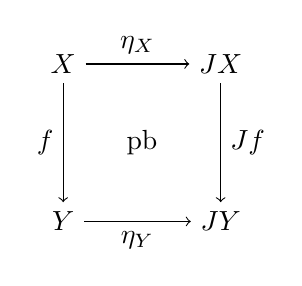
\begin{tikzpicture}
                \node (PB) at (0, 0) {pb};
                \node (X) at (-1, 1) {$X$};
                \node (JX) at (1, 1) {$\mathfrak{J}X$};
                \node (Y) at (-1, -1) {$Y$};
                \node (JY) at (1, -1) {$\mathfrak{J}Y$};
                \draw[->] (X) -- node[above]{$\eta_X$} (JX);
                \draw[->] (Y) -- node[below]{$\eta_Y$} (JY);
                \draw[->] (X) -- node[left]{$f$} (Y);
                \draw[->] (JX) -- node[right]{$\mathfrak{J}f$} (JY);
            \end{tikzpicture}
        \end{gather}
    }

    \newadef{Smooth manifold}{\index{manifold}
        A diffeological space (in its incarnation as a smooth formal set) equipped with a family of local diffeomorphisms from Euclidean spaces (also regarded as formal smooth sets) such that every point of the space lies in the image of at least one such morphism and such that the final topology induced by the plots of the smooth set is paracompact Hausdorff.
    }

    Although we started this section by claiming that we would generalize spaces to the fermionic setting, we have only constructed bosonic spaces. However, everything introduced in this section was formulated in such a way that supergeometry can be included through a minor modification:
    \newdef{Superpoint}{\index{super!point}\index{super!space}
        A space of the form $\text{Spec}(A)$ where $A:=\mathbb{R}\oplus V$ with $V$ a finite-dimensional superalgebra \ref{linalgebra:superalgebra} that forms a nilpotent ideal of $A$. When we take $A$ to be the Grassmann algebra \ref{tensor:exterior_algebra} on $n$ generators we obtain the odd space $\mathbb{R}^{0|n}$. The \textbf{super Euclidean space} $\mathbb{R}^{m|n}$ is obtained as the product of an ordinary Euclidean space $\mathbb{R}^m$ and the superpoint $\mathbb{R}^{0|n}$, i.e. its algebra of smooth functions is $C^\infty(\mathbb{R}^m\times\Pi\mathbb{R}^m)$.
    }
    \newdef{Super smooth set}{\index{smooth!set}
        A sheaf on the category of super Euclidean spaces $\mathbf{SuperCartSp_{diff}}$.
    }

\subsection{Graded manifolds}

    In this section some of the notions from Part \ref{part:diffgeom} will be generalized to the supermanifolds and even general graded manifolds. The general notation $(x^i)$ will be used for the collection of both even and odd coordinates.

    \begin{example}[Supermanifold]\index{super!manifold}
        A super smooth set in the form of a locally ringed space $(M,\mathcal{A})$ that is locally isomorphic to a super Euclidean space, i.e. $\mathcal{A}$ is locally given by $C^\infty(M)\otimes\Lambda^\bullet\mathbb{R}^n$ for some $n\in\mathbb{N}$. More generally, a \textbf{graded manifold} is a locally ringed space that is locally isomorphic to $(\mathbb{R}^m, C^\infty(\mathbb{R}^m)\otimes\text{Sym}(V^*))$ for a graded vector space $V$. (A supermanifold can be recovered by taking $V=\Pi\mathbb{R}^n$.)
    \end{example}

    \begin{theorem}[Batchelor]
        Let $(M,\mathcal{A})$ be an $\mathbb{N}$-graded manifold. There exists a vector bundle $E\rightarrow M$ such that $\mathcal{A}$ is isomorphic to the structure sheaf of $\Gamma(\Lambda^\bullet E)$, i.e. $\mathcal{A}$ is locally given by $\text{Sym}(\Lambda^\bullet E^*)$. If $(M,\mathcal{A})$ is a supermanifold, there exists a vector bundle $E\rightarrow N$ such that $\mathcal{A}$ is locally given by $\Lambda^\bullet E^*$.
    \end{theorem}

    \newdef{Vector fields}{\index{vector field}
        A graded vector field of degree $k$ is a degree-$k$ derivation on $C^\infty(M)$. The integer $k$ is called the \textbf{degree}.
    }
    \newdef{Cohomological vector field}{
        A graded vector field $X$ of degree $1$ that satisfies $[X,X]=0$. Every degree-1 graded vector field satisfies
        \begin{gather}
            [X,X] = 2X\circ X,
        \end{gather}
        which implies that every cohomological vector field defines a coboundary operator on $C^\infty(M)$.

        The de Rham complex $\Omega^\bullet(M)$ is given by $(\Pi TM, Q)$, where $Q$ is the cohomological vector field locally given by
        \begin{gather}
            Q := \sum_{i=1}^ndx^i\partial_i.
        \end{gather}
        Note that the $dx^i$ are here regarded as coordinate functions on $\Pi TM$. The \textbf{degree} of a homogeneous element of $\Omega^\bullet(M)$ is defined as the difference of its graded degree and its form degree.
    }

    \newdef{Poisson manifold}{
        Consider a degree-$k$ symplectic form $\omega$. This form induces a Poisson structure on the algebra $C^\infty(M)$ as follows:
        \begin{gather}
            \{f,g\} := f\overset{\leftarrow}{\partial_i}(\omega^{-1})^{ij}\overset{\rightarrow}{\partial_j}g.
        \end{gather}
        It is not hard to check that this operation is graded-commutative. As in Section \ref{section:hamiltonian_vector_fields}, a Hamiltonian vector field can be defined for any smooth function $H\in C^\infty(M)$:
        \begin{gather}
            \omega(X_H, \cdot) = -dH(\cdot).
        \end{gather}
    }

    \begin{property}[Euler vector field]\index{Cartan!magic formula}\index{Lie!derivative}
        Consider the graded vector field
        \begin{gather}
            E := \sum_{i=1}^n\deg(x^i)x^i\partial_i.
        \end{gather}
        The Lie derivative $\mathcal{L}_E$, defined through the Cartan formula
        \begin{gather}
            \mathcal{L}_E := \iota_Ed + (-1)^{\deg(E)}d\iota_E,
        \end{gather}
        acts on homogeneous forms by multiplication by their degree.
    \end{property}
    \begin{property}
        Every closed differential form of degree $k>0$ is exact. More generally it holds that the de Rham cohomology of a graded manifold is isomorphic to the de Rham cohomology of its body.
    \end{property}
    \begin{result}
        Consider a Hamiltonian cohomological vector field $Q$. There exists a Hamiltonian function $S$ such that
        \begin{gather}
            Qf = \{S,f\}
        \end{gather}
        for all $f\in C^\infty(M)$. If the symplectic form has degree $k$, the function $S$ can be chosen to be of degree $k+1$ and, accordingly, $\{S,S\}$ will be of degree $k+2$. Now, the identity $[Q,Q] = 0$ also implies that $\{S,S\}$ is a constant and since all constants are of degree 0, it follows that
        \begin{gather}
            \label{hdg:classical_master_equation}
            \{S,S\}=0
        \end{gather}
        whenever $k\neq-2$. This equation is often called the \textbf{classical master equation}.

        If $\omega$ if of degree 1, it was shown by \textit{Schwarz} that $(M,\omega)$ is symplectomorphic to $\Pi TM$, such that the Poisson bracket is mapped to the Schouten-Nijenhuis bracket and the Hamiltonian $S$ is mapped to a Poisson bivector field exactly if it satisfies the master equation.
    \end{result}

    \newdef{BV integral}{\index{Batalin-Vilkovisky!integral}\index{gauge}
        Consider a symplectic $m|m$-dimensional supermanifold $(M,\omega)$ where $\omega$ is odd. Let $\psi$, the \textbf{gauge fixing fermion}, be an odd function of half of the coordinates (denote these by $q$). This function determines a projectable Lagrangian submanifold $L_\psi\subset\Pi T^*\mathbb{R}^m$ by the Maslow-H\"ormander theorem \ref{symplectic:maslow_hormander}. The Batalin-Vilkovisky integral of a function $f\in C^\infty(M)$ with respect to $\psi$ is defined as
        \begin{gather}
            \int_{L_\psi}f := \left.\int f\right|_{p_i=\partial_{q^i}\psi}d^mq.
        \end{gather}

        Define the odd (BV) Laplacian as
        \begin{gather}
            \Delta_{\text{BV}} := \sum_{i=1}^m(-1)^{\deg(q^i)}\frac{\partial^2}{\partial q^i\partial p_i}.
        \end{gather}
        This operator satisfies $\Delta_{\text{BV}}f = -\frac{1}{2}\text{div}X_f$ for all $f\in C^\infty(M)$, where $\text{div}$ denotes the divergence \ref{riemann:divergence} with respect to the standard Berezinian volume form. The BV integral and BV Laplacian interact in the following way:
        \begin{enumerate}
            \item If $f=\Delta_{\text{BV}}g$, then $\int_{L_\psi}f = 0$ for all gauge fixing fermions $\psi$ (whenever the BV integral is defined).
            \item If $\Delta_{\text{BV}}f=0$, $\deriv{}{t}\int_{L_{\psi_t}}f=0$, where $\{\psi_t\}_{t\in\mathbb{R}}$ is a continuous family of gauge fixing fermions (whenever the BV integral is defined).
        \end{enumerate}
    }
    \begin{formula}[Quantum master equation]
        Consider the case of a function $f:=e^{i/\hbar S}$ where $S$ is even. Because
        \begin{gather}
            \Delta f = \frac{i}{\hbar}\Delta S e^{i/\hbar S} + \left(\frac{i}{\hbar}\right)^2\frac{1}{2}\{S,S\}e^{i/\hbar S},
        \end{gather}
        the condition that $f$ is harmonic is equivalent to $S$ satisfying
        \begin{gather}
            \frac{1}{2}\{S,S\}-i\hbar\Delta S=0.
        \end{gather}
        This equation is called the quantum master equation. Expanding $S$ as a power series in $\hbar$ shows that the constant term satisfies the classical master equation \ref{hdg:classical_master_equation}.
    \end{formula}

\section{Higher geometry}

    In this section some notions of groups, Lie groups and groupoids (Sections \ref{section:groups}, \ref{section:lie_groups} and \ref{section:groupoids} respectively) are extended the setting of higher category theory.

\subsection{Groups}

    \newdef{Lie groupoid\footnotemark}{\index{Lie!groupoid}\label{hdg:lie_groupoid}
        \footnotetext{In a similar way we could define \textit{topological groupoids, \'etal\'e groupoids}, ...}
        A groupoid internal to $\mathbf{Diff}$.

        Note that Definition \ref{cat:internal_category} requires the existence of pullbacks (of the source and target morphisms). In the category $\mathbf{Diff}$ this is equivalent to assuming that the source and target morphisms are (surjective) submersions.
    }
    \remark{In the Ehresmannian approach one gives the manifold of composable morphisms $D_1\times_{D_0}D_1$ as part of the data. Hence we do not have to assume anything about the source and target morphisms.}

    \newdef{Lie algebroid}{\index{Lie!algebroid}\index{anchor}
        A vector bundle $\pi:E\rightarrow M$ together with a vector bundle morphism $\rho:E\rightarrow TM$, called the \textbf{anchor map}, and a Lie bracket on $\Gamma(E)$ such that the following Leibniz-type property is satisfied:
        \begin{gather}
            [X, fY] = f[X, Y] + \rho(X)(f)Y.
        \end{gather}
        This property also implies that $\rho$ preserves the Lie bracket:
        \begin{gather}
            \rho([X, Y]) = [\rho(X), \rho(Y)].
        \end{gather}
    }
    \begin{example}[Tangent Lie algebroid]\index{pair!groupoid}
        The tangent bundle over a smooth manifold is a Lie algebroid with $\rho\equiv\text{id}$.

        Both the fundamental groupoid $\mathbf{\Pi_1}(M)$ (see definition \ref{topology:fundamental_groupoid}) and the pair groupoid\footnote{The objects are the elements of $M$ and between every two objects there exists exactly one morphism, i.e. $\text{hom}(\mathbf{M\times M})\equiv M\times M$.} $\mathbf{M\times M}$ integrate the tangent Lie algebroid.
    \end{example}

    One can generalize the dual construction of $L_\infty$-algebras \ref{hda:l_infinity_bis} even further:
    \newdef{$L_\infty$-algebroid}{\index{Lie!algebroid}
        Consider the construction of the Chevalley-Eilenberg algebra for a $L_\infty$-algebra. By replacing the base field by a smooth algebra $C^\infty(M)$ for some smooth manifold $M$ and the (graded) vector space $V$ by a module of sections $\Gamma(E)$ of a (graded) vector bundle $E\rightarrow M$, one obtains the notion of a $L_\infty$-algebroid.
    }
    \begin{property}
        $L_\infty$-algebras can be recovered by considering the special case $M=\{\ast\}$.
    \end{property}

    \begin{example}[de Rham complex]
        Consider the tangent algebroid of a smooth manifold $M$. The associated Chevalley-Eilenberg complex
    \end{example}

    \newdef{Weak 2-group}{\index{group!categorical}\index{2!group}
        Let $(\mathbf{C},\otimes,\mathbf{1})$ be a monoidal category. This category is called a weak 2-group, \textbf{categorical group} or \textbf{gr-category} if it satisfies the following conditions:
        \begin{itemize}
            \item All morphisms are invertible.
            \item Every object is weakly invertible with respect to the monoidal structure.
        \end{itemize}
        By property \ref{cat:monoidal_or_2} we can equivalently define a weak 2-group as a 2-category with a single object, weakly invertible 1-morphisms and invertible 2-morphisms.
    }

    \newdef{2-groupoid}{\index{2!groupoid}
        A 2-groupoid is a 2-category in which all 1-morphisms are invertible and every 2-morphisms has a ''vertical'' inverse. (The ''horizontal'' inverse can be constructed from the other ones.)
    }
    \newdef{$\infty$-groupoid}{
        A $\infty$-category in which all morphisms are invertible. This is equivalent to a $(\infty,0)$-category in the language of $(n,r)$-categories.
    }

    \newdef{Strict 2-group}{
        A (strict) 2-group is defined as a (strict) 2-groupoid with only one object. From this it follows that the set of 1-morphisms forms a group and so does the set of 2-morphisms under horizontal composition. However, the 2-morphisms do not form a group under vertical composition\footnote{Because the sources/targets may not match up.}.

        This definition is equivalent to the following internal version: a (strict) 2-group is a group object in $\mathbf{Cat}$ or an internal category in $\mathbf{Grp}$. If we replace $\mathbf{Grp}$ by $\mathbf{Lie}$ we obtain the notion of a (strict) Lie 2-group.
    }

    \begin{property}[Lie crossed modules]\index{module!crossed}\index{differential!crossed module}
        The 2-category of (strict) 2-groups is biequivalent to the 2-category of (Lie) crossed modules \ref{group:crossed_module}. Given a 2-group $\mathcal{G}$, we obtain a crossed module as follows:
        \begin{itemize}
            \item $G:=\text{ob}(\mathcal{G})$,
            \item $H:=\{h\in\text{hom}(\mathcal{G}):\mathfrak{s}(f)=e\}$,
            \item $t(h):=\mathfrak{t}(h)$, and
            \item $\alpha(g)h := \mathbbm{1}_gh\mathbbm{1}_g^{-1}$
        \end{itemize}
        where $\mathfrak{s},\mathfrak{t}$ are the source and target morphisms in $\mathcal{G}$.

        To every Lie crossed module we can also assign a \textbf{differential crossed module}. This consists of the following data:
        \begin{enumerate}
            \item two Lie algebras $\mathfrak{g},\mathfrak{h}$,
            \item a Lie algebra morphism $\partial:\mathfrak{h}\rightarrow\mathfrak{g}$, and
            \item a Lie algebra morphism $\rho:\mathfrak{g}\rightarrow\text{Der}(\mathfrak{h})$.
        \end{enumerate}
        The equivariance and Peiffer conditions induce similar conditions for the above data:
        \begin{itemize}
            \item $\partial(\rho(h)g) = [h,\partial g]$, and
            \item $\rho(\partial h)(h') = [h,h']$
        \end{itemize}
        where $g\in\mathfrak{g}$ and $h,h'\in\mathfrak{h}$. The biequivalence of crossed modules and strict 2-groups induces a biequivalence of differential crossed modules and strict Lie 2-algebras.
    \end{property}

    \begin{example}[Automorphism 2-group]
        Given a Lie group $H$, we can construct a crossed module with $G:=\text{Aut}(H)$, $t$ assigning inner automorphisms (conjugations) and $\alpha$ the obvious map. The associated 2-group $\text{AUT}(H)$ gives a 2-group of symmetries of $H$, i.e. it is the automorphism 2-group of $H$ in the 2-category $\mathbf{Lie}$.
    \end{example}

    \newdef{Exponentiable groups}{\index{exponentiable}
        Smooth groups for which every smooth function $f:[0,1]\rightarrow\mathfrak{g}$ corresponds to a smooth function $g:[0,1]\rightarrow G$ such that
        \begin{gather}
            \deriv{}{t}g(t) = f(t)g(t)
        \end{gather}
        with $g(0) = e$, are said to be exponentiable. A smooth 2-group is said to be exponentiable if both of its component groups are exponentiable. Since all Lie groups are exponentiable, all Lie 2-groups are also exponentiable
    }

    \begin{remark}[Lie's third theorem]\index{Lie!third theorem}
        In ordinary Lie theory Lie's third theorem states that every (finite-dimensional) Lie algebra can be obtained as the infinitesimal version of a Lie group. However, this does not carry over to the 2-group setting. Consider for example the Lie 2-algebras $\mathfrak{g}_\lambda$ constructed in example \ref{hda:gk_lie_2_algebra}. As shown in \cite{HDA5} only $\mathfrak{g}_0$ gives rise to a Lie 2-group (or even a topological 2-group).
    \end{remark}

\subsection{Spaces}

    \newdef{Smooth 2-space}{
        To overcome the problem encountered in definition \ref{hdg:lie_groupoid} above, we should pass from $\mathbf{Diff}$ to $\mathbf{C^\infty}$. It can be shown that this category admits all pullbacks, quotients, path spaces, etc. As such we define a smooth 2-space as a category internal to $\mathbf{C^\infty}$.

        In the remainder of this chapter we will assume all spaces to be smooth in the general sense. The notions of 2-groups as introduced in the previous section are easily generalized to this wider setting.
    }

    \newdef{2-group action}{\index{group!action}
        Consider a smooth 2-group $\mathcal{G}$ and a smooth 2-space $E$. A strict action of $\mathcal{G}$ on $E$ is a smooth homomorphism $\mathcal{G}\rightarrow\text{AUT}(E)$, i.e. a smooth map preserving products and inverses.
    }

    \newdef{Thin homotopy}{\index{homotopy!thin}
        Let $M$ be a smooth manifold. A smooth homotopy $H:[0,1]^2\rightarrow M$ is said to be thin if
        \begin{gather}
            H(s, t) = F(s)
        \end{gather}
        for some smooth $F$ near $t=0,1$ and if it pulls back\footnote{See section \ref{section:forms}.} every two-form to 0:
        \begin{gather}
            \forall \omega\in\Omega^2(M): H^*\omega = 0.
        \end{gather}
    }
    \newdef{Lazy path\footnotemark}{\index{path!lazy}\index{sitting instants}
        \footnotetext{Also called a path with \textbf{sitting instants}.}
        Let $M$ be a smooth manifold. A path $f:[0,1]\rightarrow M$ is said to be lazy if it is locally constant on some neighbourhoods of $0$ and $1$.
    }

    \newdef{Path groupoid}{\index{groupoid!path}\label{hdg:path_groupoid}
        Let $M$ be a smooth space. The path groupoid $\mathcal{P}_1(M)$ is the groupoid (in fact a smooth groupoid and hence a smooth 2-group) which has the points of $M$ as objects and the thin homotopy classes of lazy paths with fixed endpoints on $M$ as morphisms.\footnote{The laziness combined with the first condition of thin homotopies implies that the morphisms of the groupoid are (locally) constant near the full boundary of their domain.}

        In fact by suitably generalizing the smoothness properties of the homotopies and paths, we can ''easily'' extend this definition to surface, volumes and so on. This results in the $n$-path $n$-groupoid $\mathcal{P}_n(M)$.
    }
    \sremark{The restriction to lazy paths is required to ensure the smoothness of composite paths. The quotient by thin homotopies is required to ensure the validity of the associativity and invertibility properties.}

    ?? COMPLETE ??

\section{2-Bundles}

    A first step is the generalization of the categorical definition of a bundle \ref{diff:bundle}, i.e. as an object of a slice category:
    \newdef{2-bundle}{\index{bundle}
        A smooth 2-bundle is a triple $(E,B,\pi)$ where both $E$ and $B$ are smooth 2-spaces and $\pi$ is a smooth map.
    }
    \newdef{Locally trivial 2-bundle}{
        For a smooth 2-space we define a locally trivial 2-bundle with typical fibre $F$ as a 2-bundle $(E,B,\pi)$ with an open cover $\{U_i\}_{i\in I}$ of $B$ such that for every $i\in I$ there exists an equivalence $\varphi_i:E|_{U_i}\cong U_i\times F$ that makes the diagram below commute.

        \begin{figure}[ht!]
            \centering
            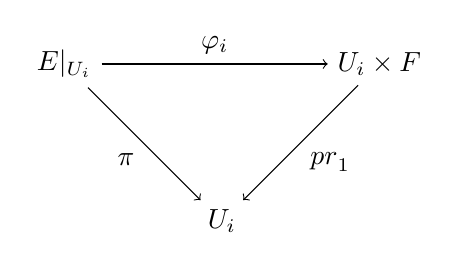
\begin{tikzpicture}
                \node (E) at (-2, 0) {$E|_{U_i}$};
                \node (UF) at (2, 0) {$U_i\times F$};
                \node (U) at (0, -2) {$U_i$};
                \draw[->] (E) -- node[above]{$\varphi_i$} (UF);
                \draw[->] (E) -- node[below left]{$\pi$} (U);
                \draw[->] (UF) -- node[below right]{$\text{pr}_1$} (U);
            \end{tikzpicture}
        \end{figure}
        We should note that the existence of such a cover is not a trivial matter. The general definition becomes quite involved when allowing for arbitrary smooth 2-spaces $B$. For convenience we will always assume that $B$ is an ordinary smooth space regarded as a 2-space with only trivial morphisms.

        As was the case in definition \ref{diff:fibre_bundle}, we can also characterize locally trivial 2-bundles by their transition data. Since the trivilizations $\varphi_i$ are equivalences, they admit an inverse (up to an invertible 2-map) and we can thus construct transition maps $\varphi_i\varphi_j^{-1}=U_{ij}\times F\cong U_{ij}\times F$ as usual. By the commutative diagram above, these transition maps only act on the fibre $F$. Because $\varphi_i\varphi_j^{-1}$ is itself an (auto)equivalence, the action on $F$ is given by a functor $g_{ij}:U_{ij}\rightarrow\text{AUT}(F)$ where the 2-space $\text{AUT}(F)$ is the \textit{coherent }2-\textit{group}\footnote{Instead of the strict invertibility of maps in our definition of 2-groups, we should allow them to be invertible up to 2-isomorphisms which themselves satisfy certain coherence conditions.} of autoequivalences of $F$ together with invertible 2-maps between them.

        The interesting (and important) part is how the cocycle conditions \ref{diff:G_cocycle_condition} and \ref{diff:G_cocycle_conditions} for the maps $g_{ij}$ are modified. Since the equivalences $g_{ij}$ are only invertible up to 2-maps, we cannot expect these conditions to hold as equations. Instead we obtain 2 higher transition maps (i.e. natural isomoprhisms) $h_{ijk}:g_{ij}\circ g_{jk}\Rightarrow g_{ik}$ and $k_i:g_{ii}\Rightarrow\text{id}$. These higher data should in turn satisfy the necessary conditions coming from associativity and unitality constraints (similar to the coherence conditions in section \ref{section:hda_group_cohomology}).
    }
    \newdef{$\mathcal{G}$-bundle}{\index{principal!bundle}
        A locally trivial 2-bundle with typical fibre $F$ is said to have the 2-group $\mathcal{G}$ as its structure (2-)group if the transition data factor through an action $\mathcal{G}\rightarrow\text{AUT}(F)$. If $F=\mathcal{G}$, we call the 2-bundle a \textbf{principal $\mathcal{G}$-2-bundle}.
    }
    \begin{remark}[Gerbes]\index{gerbe}
        If we choose the transition maps $k_i$ to be trivial and let $\mathcal{G}$ be respectively the trivial Lie 2-group associated to an Abelian Lie group $G$ or the automorphism 2-group of a Lie group $H$, we obtain Abelian and non-Abelian \textit{gerbes}. In fact it can be shown that the 2-category of principal $2$-bundles is equivalent to the 2-category of gerbes for every Lie 2-group of the aforementioned type.
    \end{remark}

    By categorifying definition \ref{diff:holonomy_functor} of principal connections we can define connections for principal $n$-bundles:
    \newdef{$n$-connection}{\index{connection!principal}
        Let $M$ be a smooth space and let $G$ be a Lie $n$-groupoid. Given a locally trivial principal $n$-bundle $P$ over $M$ we define an $n$-connection with $n$-holonomy through the following data:
        \begin{enumerate}
            \item for every coordinate chart $U_i\subset M$ a local holonomy $n$-functor
            \begin{gather}
                \text{hol}_i:\mathcal{P}_n(U_i)\rightarrow G;
            \end{gather}
            \item for every double intersection $U_{ij}$ a 1-transfor (i.e. an $n$-natural transformation)
            \begin{gather}
                g_{ij}:\text{hol}_i\Rightarrow\text{hol}_j;
            \end{gather}
            \item for every triple intersection $U_{ijk}$ a 2-transfor
            \begin{gather}
                f_{ijk}:g_{ij}\circ g_{jk}\Rrightarrow g_{ik};
            \end{gather}
            \item and so on...
        \end{enumerate}
        This is equivalently given by a global $n$-functor
        \begin{gather}
            \text{hol}:\mathcal{P}_n(M)\rightarrow\mathbf{Trans}_n(P).
        \end{gather}
    }

    ?? ADD GERBES (e.g. BRYLINSKI) AND PERHAPS DELIGNE COHOMOLOGY ??

\section{Space and quantity}

    In this section we move our focus back from (differential) geometry to the general notion of what spaces and observables are. From the start we will assume that we are working in an enriched setting where $\mathcal{V}$ is a cosmos \ref{cat:cosmos}. The categories $\mathbf{C}$ of interest will be assumed to be small and $\mathcal{V}$-enriched.

    In the previous sections we defined spaces modelled on a base space $X$, or more generally on a category of spaces $\mathbf{S}$, as sheaf or even a concrete sheaf on a suitable site. Here we relax this notion as much as possible:
    \newdef{Space}{\index{space}
        A (generalized) space modelled on a category $\mathbf{C}$ is a presheaf on $\mathbf{C}$.

        As before we can interpret the object $X(C)$ as the collection of ''probes'' from $C$ to $X$. The Yoneda lemma and embedding assure that ordinary test spaces in $\mathbf{C}$ can be viewed as spaces modelled on $\mathbf{C}$ and that their probes are indeed the ordinary maps in $\mathbf{C}$.
    }
    In a similar vein we can define observables as maps out of a space:
    \newdef{Quantity}{\index{quantity}
        A (generalized\footnote{It is generalized because it is ''measured'' on category instead of on a single object.}) quantity on a category $\mathbf{C}$ is a copresheaf on $\mathbf{C}$.
    }

    \begin{property}[Isbell duality]\index{Isbell duality}
        Given a space $X$ we can look at the quantities that live on it (in ordinary geometry this would have been its algebra of functions). This defines a functor:
        \begin{gather}
            \mathcal{O}:\mathbf{Psh(C)}\rightarrow\mathbf{coPsh}^{op}(\mathbf{C}):X\mapsto\hom_{\mathbf{Psh(C)}}(X, \mathcal{Y}-).
        \end{gather}
        Similarly, given a quantity $Q$ we can ask on which space it behaves as the algebra of functions. This also defines as functor:
        \begin{gather}
            \text{Spec}:\mathbf{coPsh}^{op}(\mathbf{C})\rightarrow\mathbf{Psh(C)}:Q\mapsto\hom_{\mathbf{coPsh(C)}}(\mathcal{Y}^{op}-, Q)
        \end{gather}
        where $\mathcal{Y}^{op}$ denotes the co-Yoneda embedding $\mathbf{C}\rightarrow\funccat{C}{\mathcal{V}}^{op}:c\mapsto\mathbf{C}(, -)$.

        The incredible result is now that $(\mathcal{O}\dashv\text{Spec})$ is an adjunction (suitably called the \textbf{Isbell adjunction}). Objects that are preserved (up to isomorphism) under the associated (co)monad are said to be \textbf{Isbell self-dual}.
    \end{property}
    \begin{example}[Cartesian spaces]
        When working over the site $\mathbf{CartSp}$ (with its usual topology) and restrict to coherent sheaves and product-preserving presheaves, the Isbell adjunction maps spaces to smooth algebras.
    \end{example}

\part{Probability Theory \& Statistics}
\chapter{Probability}\label{chapter:probability}

    The majority of this chapter uses the language of measure theory. For an introduction see Chapter \ref{chapter:measure}.

\section{Probability}

    The Kolmogorov axioms of probability state when a set admits the definition of a probability theory:
    \newdef{Kolmogorov axioms}{\index{Kolmogorov!axioms}\index{probability}\index{sample space}
        A probability space $(\Omega,\Sigma,P)$ is a measure space \ref{lebesgue:measure_space} with finite measure $P(X)=1$. The set $\Omega$ is called the \textbf{sample space}.
    }

    \newdef{Random variable}{\index{random variable}
        Let $(\Omega,\Sigma,P)$ be a probability space. A function $X:\Omega\rightarrow\mathbb{R}$ is called a random variable if $\forall a\in\mathbb{R}:X^{-1}\big([a,+\infty[\big)=\{\omega\in\Omega\mid X(\omega)\geq a\}\in\Sigma$.
    }

    \newdef{$\sigma$-algebra of a random variable}{\index{$\sigma$!algebra}
        Let $X$ be a random variable defined on a probability space $(\Omega,\Sigma,P)$. The following family of sets is a $\sigma$-algebra:
        \begin{gather}
            \label{prob:sigma_algebra_generated_random_variable}
            X^{-1}(\mathcal{B}) := \{S\in\Sigma\mid\exists B\in\mathcal{B}:S = X^{-1}(B)\}.
        \end{gather}
    }
    \begin{notation}
        The $\sigma$-algebra generated by the random variable $X$ is often denoted by $\mathcal{F}_X$, analogous to \ref{set:notation:generated_sigma_algebra}.
    \end{notation}

    \newdef{Event}{\index{event}
        Let $(\Omega,\Sigma,P)$ be a probability space. An element $S$ of the $\sigma$-algebra $\Sigma$ is called an event.

        From this definition it is clear that a single possible outcome of a measurement can be a part of multiple events. So, although only one outcome can occur at the same time, multiple events can occur simultaneously.
    }
    \begin{remark*}
        The Kolmogorov axioms use the $\sigma$-algebra \ref{set:sigma_algebra} of events instead of the power set \ref{set:power_set} of all events. Intuitively this seems to mean that some possible outcomes are not treated as events. However, one can make sure that the $\sigma$-algebra still contains all ``useful'' events by using a ``nice'' definition of probability spaces.
    \end{remark*}

    \begin{formula}[Union]\label{prob:union}
        Let $A,B$ be two events. The probability that at least one of them occurs is given by the following formula:
        \begin{gather}
            P(A\cup B) = P(A) + P(B) + P(A\cap B).
        \end{gather}
    \end{formula}

    \newdef{Disjoint events}{
        Two events $A$ and $B$ are said to be disjoint if they cannot happen at the same time:
        \begin{gather}
            P(A\cap B) = 0.
        \end{gather}
    }
    \result{If $A$ and $B$ are disjoint, the probability that both $A$ and $B$ occur is just the sum of their individual probabilities.}

    \newformula{Complement}{\index{complement}\label{prob:complement}
        Let $A$ be an event. The probability of $A$ being false is denoted as $P\left(\overline{A}\right)$ and is given by
        \begin{gather}
            P\left(\overline{A}\right) = 1 - P(A).
        \end{gather}
    }
    \begin{result}
        From the previous equation and de Morgan's laws \eqref{set:de_morgan_union} and \eqref{set:de_morgan_intersection}, one can derive the following formula:
        \begin{gather}
            P\left(\overline{A}\cap\overline{B}\right) = 1 - P(A\cup B).
        \end{gather}
    \end{result}

\section{Conditional probability}

    \newdef{Conditional probability}{\index{probability!conditional}\label{prob:conditional_probability}
        Let $A,B$ be two events. The probability of $A$ given that $B$ is true is denoted as $P(A|B)$:
        \begin{gather}
            P(A|B) = \stylefrac{P(A\cap B)}{P(B)}.
        \end{gather}
    }
    By interchanging $A$ and $B$ in previous equation and by observing that this has no effect on the quantity $P(A\cap B)$ the following important result can be derived:
    \begin{theorem}[Bayes]\index{Bayes}\label{prob:bayes}
        Let $A,B$ be two events.
        \begin{gather}
            P(A|B) = \frac{P(B|A)P(A)}{P(B)}.
        \end{gather}
    \end{theorem}

    \begin{formula}
        Let $\seq{B}$ be a sequence of pairwise disjoint events. If $\bigsqcup_{n=1}^\infty B_n = \Omega$, the total probability of a given event $A$ can be calculated as follows:
        \begin{gather}
            \label{probability:total_probability_conditional}
            P(A) = \sum_{n=1}^\infty P(A|B_n)P(B_n).
        \end{gather}
    \end{formula}

    \newdef{Independent events}{\index{independence}
        Let $A,B$ be two events. $A$ and $B$ are said to be independent if they satisfy the following relation:
        \begin{gather}
            P(A\cap B) = P(A)P(B).
        \end{gather}
    }
    \begin{result}
        If $A$ and $B$ are two independent events, Bayes's theorem simplifies to
        \begin{gather}
            P(A|B) = P(A).
        \end{gather}
    \end{result}
    The above definition can be generalized to multiple events:
    \begin{definition}
        The events $A_1,\ldots,A_n$ are said to be independent if for each choice of $k$ events the probability of their intersection is equal to the product of their individual probabilities.
    \end{definition}
    This definition can be stated in terms of $\sigma$-algebras:
    \begin{definition}[Independence]\index{independence}
        The $\sigma$-algebras $\mathcal{F}_1,\ldots,\mathcal{F}_n$ defined on a probability space $(\Omega,\mathcal{F},P)$ are said to be independent if for all choices of distinct indices $i_1,\ldots,i_k$ and for all choices of sets $F_{i_n}\in\mathcal{F}_{i_n}$ the following equation holds:
        \begin{gather}
            \label{prob:independent_sigma_algebras}
            P(F_{i_1}\cap\cdots\cap F_{i_k}) = P(F_{i_1})\cdots P(F_{i_k}).
        \end{gather}
    \end{definition}
    \begin{result}
        Let $X,Y$ be two random variables. $X$ and $Y$ are independent if the $\sigma$-algebras generated by them are independent.
    \end{result}

\section{Probability distribution}

    \newdef{Probability distribution}{\index{probability!distribution}\label{prob:probability_distribution}
        Let $X$ be a random variable defined on a probability space $(\Omega,\Sigma,P)$. The following function is a measure on the Borel $\sigma$-algebra of $\mathbb{R}$:
        \begin{gather}
            P_X(B) = P(X^{-1}(B)).
        \end{gather}
        This measure is called the probability distribution of $X$.
    }

    \newdef{Density}{\index{density}\index{cumulative distribution function}
        \nomenclature[A_CDF]{CDF}{cumulative distribution function}
        Let $f\geq0$ be an integrable function and recall Property \ref{lebesgue:measure_by_integral}. The function $f$ is called the density of the measure $P(A):=\int_Af\,d\lambda$ (with respect to the Lebesgue measure $\lambda$). Measures of this form are often called \textbf{cumulative distribution functions} and denoted by $F$. More generally, by the Radon-Nikodym theorem from Section \ref{section:Radon-Nikodym}, every absolutely continuous distribution function $F$ is of the form
        \begin{gather}
            F(A) = \int_Af\,d\lambda
        \end{gather}
        for some integrable function $f$.
    }

    \begin{theorem}[Skorokhod's representation theorem]\index{Skorokhod}
        Let $F:\mathbb{R}\rightarrow[0,1]$ be a function that satisfies the following three properties:
        \begin{itemize}
            \item $F$ is nondecreasing.
            \item $\ds\lim_{x\rightarrow-\infty}F(x) = 0$ and $\ds\lim_{x\rightarrow\infty}F(x) = 1$.
            \item $F$ is right-continuous, i.e. $\ds\lim_{y\nearrow y_0}F(y)=F(y_0)$.
        \end{itemize}
        There exists a random variable $X:[0,1]\rightarrow\mathbb{R}$ defined on the probability space $([0,1],\mathcal{B},m_{[0,1]})$ such that $F=F_X$.
    \end{theorem}

    \begin{theorem}[Theorem of the unconscious statistician]\label{prob:unconscious_statistician}
        Consider a random variable $X$ on a probability space $(\Omega,\Sigma,P)$. The following equality holds for every integrable function $g\in L^1(\mathbb{R})$:
        \begin{gather}
            \int_\Omega g\circ X\,dP = \int_\mathbb{R}g(x)dP_X(x).
        \end{gather}
    \end{theorem}
    \begin{remark}
        The name of this theorem stems from the fact that many scientists take this equality to be a definition of the expectation value $\text{E}[g(X)]$. However, this equality should be proven since the measure on the right-hand side is the one belonging to the random variable $X$ and not $g(X)$.
    \end{remark}

    \begin{formula}
        Consider an absolutely continuous probability function $F$ defined on $\mathbb{R}^n$ and let $f$ be the associated density. Let $g:\mathbb{R}^n\rightarrow\mathbb{R}$ be integrable with respect to $F$.
        \begin{gather}
            \int_{\mathbb{R}^n}g\,dF = \int_{\mathbb{R}^n}f(x)g(x)dx
        \end{gather}
    \end{formula}
    \begin{result}
        The previous formula together with Theorem \ref{prob:unconscious_statistician} gives rise to
        \begin{gather}
            \label{prob:omega_int_to_real_int}
            \int_\Omega g\circ X\,dP = \int_{\mathbb{R}^n}f_X(x)g(x)dx.
        \end{gather}
    \end{result}

    \begin{formula}
        Let $X$ be a random variable with density function $f_X$ and let $g:\mathbb{R}\rightarrow\mathbb{R}$ be smooth and strictly monotone. The random variable $g\circ X$ has an associated density $f_g$ given by
        \begin{gather}
            \label{prob:function_of_random_variable}
            f_g(y) = f(g^{-1}(y))\left|\deriv{g^{-1}}{y}(y)\right|.
        \end{gather}
    \end{formula}

    \newdef{Convergence in distribution}{\index{convergence!in distribution}
        A sequence $\seq{X}$ of random variables is said to converge in distribution to a random variable $Y$ if the associated distribution functions $F_{X_n}$ converge pointwise to $F_Y$, i.e. $\lim_{n\rightarrow\infty}F_{X_n}(x)=F_Y(x)$ for all $x\in\mathbb{R}$.
    }
    \begin{notation}
        If a sequence $\seq{X}$ converges in distribution to a random variable $Y$, this is often denoted by $X_n\overset{d}{\longrightarrow}Y$. Sometimes the $d$ (for ``distribution'') is replaced by the $\mathcal{L}$ (for ``law'').
    \end{notation}

    \begin{theorem}[Slutsky]\index{Slutsky}
        Let $\seq{X},\seq{Y}$ be two sequences of random variables converging in probability to a random variable $X$ and a constant $c$, respectively. The following statements hold:
        \begin{itemize}
            \item $X_n+Y_n\overset{d}{\longrightarrow}X+c$,
            \item $X_nY_n\overset{d}{\longrightarrow}cX$, and
            \item $X_n/Y_n\overset{d}{\longrightarrow}X/c$.
        \end{itemize}
    \end{theorem}

    \newdef{\difficult{Giry monad}}{\index{Giry monad}
        Consider the category $\mathbf{Meas}$ of measurable spaces. On this space one can define a monad \ref{cat:monad} that sends a set $X$ to its collection of probability distributions equipped with the $\sigma$-algebra generated by all evaluation maps $\mathrm{ev}_U$, where $U$ runs over the measurable subsets of $X$.

        The unit of the Giry monad $G$ is defined by assigning Dirac measures:
        \begin{gather}
            \eta_X(x) := \delta_x.
        \end{gather}
        The multiplication map is defined as follows:
        \begin{gather}
            \mu_X(Q)(U) := \int_{P\in GX}\mathrm{ev}_U(P)\,dQ.
        \end{gather}
    }

\section{Moments}
\subsection{Expectation value}

    \newdef{Expectation value}{\index{expectation}\label{prob:expectation_value}
        Let $X$ be random variable defined on a probability space $(\Omega,\Sigma,P)$.
        \begin{gather}
            \expect{X} := \int_\Omega X\,dP
        \end{gather}
    }
    \begin{notation}
        Other notations that are common in the literature are $\langle X \rangle$ and $\mu_X$.
    \end{notation}

    \newdef{Moment of order \texorpdfstring{$r$}{r}}{\index{moment}\label{prob:moment}
        The moment of order $r$ is defined as the expectation value of the $r^{th}$ power of $X$. By Equation \eqref{prob:omega_int_to_real_int} this becomes
        \begin{gather}
            \expect{X^r} = \int_\mathbb{R}x^rf_X(x)dx.
        \end{gather}
    }
    \newdef{Central moment of order \texorpdfstring{$r$}{r}}{\index{central!moment}\label{prob:central_moment}
        \begin{gather}
            \expect{(X-\mu)^r} = \int_\mathbb{R}(x-\mu)^rf_X(x)dx
        \end{gather}
    }
    \begin{remark}
        Moments of order $n$ are determined by central moments of order $k\leq n$ and, conversely, central moments of order $n$ are determined by moments of order $k\leq n$.
    \end{remark}
    \newdef{Variance}{\index{variance}
        The central moment of order 2 is called the variance:
        \begin{gather}
            \variance{X} := \expect{(X-\mu)^2}.
        \end{gather}
    }
    \newdef{Standard deviation}{\index{standard!deviation}
        \begin{gather}
            \sigma_X := \sqrt{V[X]}
        \end{gather}
    }

    \begin{property}
        If $\expect{|X|^n}$ is finite for $n>0$, then $\expect{X^k}$ exist and is finite for all $k\leq n$.
    \end{property}

    \newdef{Moment generating function}{\index{moment!generating function}\label{prob:moment_generating_function}
        \begin{gather}
            M_X(t) := \expect{e^{tX}} = \int_{-\infty}^\infty e^{tx}f_X(x)dx
        \end{gather}
    }
    \begin{property}
        If the moment generating function exists, the moments $\expect{X^n}$ can be expressed in terms of $M_X$ (using the series expansion of the exponential function):
        \begin{gather}
            \label{prob:moment_generating}
            \expect{X^n} = \left.\mderiv{n}{M_X(t)}{t}\right|_{t=0}.
        \end{gather}
    \end{property}

    \newdef{Characteristic function}{\index{characteristic!function}\label{prob:characteristic_function}
        \begin{gather}
            \varphi_X(t) := \expect{e^{itX}}
        \end{gather}
    }
    \begin{property}\label{prob:characteristic_function_properties}
        The characteristic function has the following properties:
        \begin{itemize}
            \item $\varphi_X(0) = 1$,
            \item $|\varphi_X(t)| \leq 1$, and
            \item $\varphi_{aX+b}(t) = e^{itb}\varphi_X(at)$ for all $a,b\in\mathbb{R}$.
        \end{itemize}
    \end{property}

    \begin{formula}
        If $\varphi_X(t)$ is $k$ times continuously differentiable, then $X$ has a finite $k^{th}$ moment and
        \begin{gather}
            \label{prob:characteristic_function_as_moment_generator}
            \expect{X^k} = \frac{1}{i^k}\mderiv{k}{}{t}\varphi_X(0).
        \end{gather}
        Conversely, if $X$ has a finite $k^{th}$ moment, then $\varphi_X(t)$ is $k$ times continuously differentiable and the above formula holds.
    \end{formula}

    \newformula{Inversion formula}{\index{inversion!formula}
        Let $X$ be a random variable. If the CDF of $X$ is continuous at $a,b\in\mathbb{R}$, then
        \begin{gather}
            \label{prob:inversion_formula}
            F_X(b) - F_X(a) = \lim_{c\rightarrow\infty}\frac{1}{2\pi}\int_{-c}^c\frac{e^{-ita} - e^{-itb}}{it}\varphi_X(t)dt.
        \end{gather}
    }
    \begin{formula}
        If $\varphi_X(t)$ is integrable, the CDF is given by:
        \begin{gather}
            f_X(x) = \frac{1}{2\pi}\int_{-\infty}^\infty e^{-itx}\varphi_X(t)dt.
        \end{gather}
    \end{formula}
    \remark{This formula implies that the density function and the characteristic function form a Fourier transform pair.}

\subsection{Correlation}

    \begin{property}\index{independence}\label{prob:independence_expectation_values}
        Two random variables $X,Y$ are independent if and only if $\expect{f(X)g(Y)} = \expect{f(X)}\expect{g(Y)}$ holds for all Borel-measurable bounded functions $f,g$.
    \end{property}

    The value $\expect{XY}$ is equal to the inner product $\langle X|Y \rangle$ as defined in \eqref{lebesgue:L2_inner_product}. It follows that independence of random variables implies orthogonality. To generalize this concept, the following notions are introduced:
    \newdef{Centred random variable}{\index{random variable}
        Let $X$ be a random variable with finite expectation value $\expect{X}$. The centred random variable $X_c$ is defined as $X_c = X-\expect{X}$.
    }
    \newdef{Covariance}{\index{covariance}
        The covariance of two random variables $X,Y$ is defined as follows:
        \begin{gather}
            \label{prob:covariance}
            \mathrm{cov}(X,Y) := \langle X_c|Y_c \rangle = \expect{(X-\expect{X})(Y-\expect{Y})}.
        \end{gather}
        Some basic math gives
        \begin{gather}
            \mathrm{cov}(X,Y) = \expect{XY} - \expect{X}\expect{Y}.
        \end{gather}
    }
    \newdef{Correlation}{\index{correlation}\label{prob:correlation}
        The correlation of two random variables $X,Y$ is defined as the cosine of the angle between $X_c$ and $Y_c$:
        \begin{gather}
            \rho_{XY} := \frac{\mathrm{cov}(X,Y)}{\sigma_X\sigma_Y}.
        \end{gather}
    }
    \result{From Theorem \ref{prob:independence_expectation_values} it follows that independent random variables are uncorrelated.}
    \result{If the random variables $X$ and $Y$ are uncorrelated, they satisfy $\expect{XY} = \expect{X}\expect{Y}$.}

    \begin{formula}[Bienaym\'e formula]\index{Bienaym\'e}\label{prob:bienayme}
        Let $\seq{X}$ be a sequence of independent (or uncorrelated) random variables. Their variances satisfy the following equation:
        \begin{gather}
            \label{prob:variance_of_sum}
            \variance{\sum_{i=1}^\infty X_i} = \sum_{i=1}^\infty\variance{X_i}.
        \end{gather}
    \end{formula}

\subsection{Conditional expectation}

    Let $(\Omega,\Sigma,P)$ be a probability space. Consider a random variable $X\in L^2(\Omega,\Sigma,P)$ and a sub-$\sigma$-algebra $\mathcal{G}\subset\Sigma$. Property \ref{lebesgue:L2_hilbert_space} implies that the spaces $L^2(\Sigma)$ and $L^2(\mathcal{G})$ are complete and, hence, the projection theorem \ref{functional:projection_theorem} can be applied. For every $X\in L^2(\Sigma)$ there exists a random variable $Y\in L^2(\mathcal{G})$ such that $X-Y$ is orthogonal to $L^2(\mathcal{G})$. This has the following result:
    \begin{gather}
        \forall Z\in L^2(\mathcal{G}):\langle X-Y|Z \rangle\equiv\int_\Omega(X-Y)ZdP = 0.
    \end{gather}
    Since $\mathbbm{1}_G\in L^2(\mathcal{G})$ for every $G\in\mathcal{G}$, Equation \eqref{lebesgue:domain_change} can be rewritten as
    \begin{gather}
        \label{prob:conditional_expectation_condition}
        \int_GX\,dP = \int_GY\,dP
    \end{gather}
    for all $G\in\mathcal{G}$. This leads to the introduction of the following definition:
    \newdef{Conditional expectation}{\index{expectation!conditional}\label{prob:conditional_expectation}
        Let $(\Omega,\Sigma,P)$ be a probability space and let $\mathcal{G}$ be a sub-$\sigma$-algebra of $\Sigma$. For every $\Sigma$-measurable random variable $X\in L^2(\Sigma)$ there exists a unique (up to a null set) random variable $Y\in L^2(\mathcal{G})$ that satisfies Equation \eqref{prob:conditional_expectation_condition} for every $G\in\mathcal{G}$. This variable $Y$ is called the conditional expectation of $X$ given $\mathcal{G}$ and it is denoted by $\expect{X|\mathcal{G}}$:
        \begin{gather}
            \int_G\expect{X|\mathcal{G}}\,dP = \int_GX\,dP.
        \end{gather}
    }
    \begin{remark}
        Although this construction was based on orthogonal projections, one could as well have used the (signed) Radon-Nikodym theorem \ref{lebesgue:signed_radon_nikodym} since $G\mapsto\int_GX\,dP$ is absolutely continuous with respect to $P|_{\mathcal{G}}$.
    \end{remark}

    \begin{property}\label{prob:conditional_expectation_props}
        Let $(\Omega,\Sigma,P)$ be a probability space and consider a sub-$\sigma$-algebra $\mathcal{G}\subset\Sigma$. If the random variable $X$ is $\mathcal{G}$-measurable, then
        \begin{gather}
            \expect{X|\mathcal{G}} = X\text{ a.s.}
        \end{gather}
        On the other hand, if $X$ is independent of $\mathcal{G}$, then
        \begin{gather}
            \expect{X|\mathcal{G}} = \expect{X}\text{ a.s.}
        \end{gather}
    \end{property}

\section{Joint distributions}

    \newdef{Joint distribution}{\index{distribution!joint}
        Let $X,Y$ be two random variables defined on the same probability space $(\Omega,\Sigma,P)$ and consider the vector random variable $(X,Y):\Omega\rightarrow\mathbb{R}^2$. The distribution of $(X,Y)$ isa probability measure defined on the Borel algebra of $\mathbb{R}^2$ defined by
        \begin{gather}
            P_{(X,Y)}(B) = P((X,Y)^{-1}(B)).
        \end{gather}
    }
    \newdef{Joint density}{
        If the probability measure from the previous definition can be written as
        \begin{gather}
            P_{(X,Y)}(B) = \int_Bf_{(X,Y)}(x,y)dxdy
        \end{gather}
        for some integrable $f_{(X,Y)}$, it is said that $X$ and $Y$ have a joint density.
    }

    \newdef{Marginal distribution}{\index{distribution!marginal}
        The distributions of the one-dimensional random variables is determined by the joint distribution:
        \begin{gather}
            P_X(A) = P_{(X,Y)}(A\times\mathbb{R})\\
            P_Y(A) = P_{(X,Y)}(\mathbb{R}\times A).
        \end{gather}
    }
    \begin{result}
        If the joint density exists, the marginal distributions are absolutely continuous and the associated density functions are given by
        \begin{gather}
            f_X(x) = \int_\mathbb{R}f_{(X,Y)}(x,y)dy\\
            f_Y(y) = \int_\mathbb{R}f_{(X,Y)}(x,y)dx.
        \end{gather}
        The converse, however, is not always true. The one-dimensional distributions can be absolutely continuous without the existence of a joint density.
    \end{result}

    \begin{property}[Independence]\index{independence}\label{prob:independent_densities}
        Let $X,Y$ be two random variables with joint distribution $P_{(X,Y)}$. $X$ and $Y$ are independent if and only if the joint distribution coincides with the product measure:
        \begin{gather}
            P_{(X,Y)} = P_X\otimes P_Y.
        \end{gather}
        If $X$ and $Y$ are absolutely continuous, the previous properties also applies to the densities instead of the distributions.
    \end{property}

    \begin{formula}[Sum of random variables]
        Consider two independent random variables $X,Y$ and let $Z=X+Y$ denote their sum. The density $f_Z$ is given by the following convolution:
        \begin{gather}
            f_Z(z) := f\ast g(z) = \int_{-\infty}^\infty g(x)h(z-x)dx = \int_{-\infty}^\infty g(z-y)h(y)dy,
        \end{gather}
        where $g,h$ denote the densities of $X,Y$ respectively.
    \end{formula}
    \begin{formula}[Product of random variables]
        Consider two independent random variables $X,Y$ and let $Z=XY$ denote their product. The density $f_Z$ is given by
        \begin{gather}
            f_Z(z) = \int_{-\infty}^\infty g(x)h(z/x)\frac{dx}{|x|} = \int_{-\infty}^\infty g(z/y)h(y)\frac{dy}{|y|},
        \end{gather}
        where $g,h$ denote the densities of $X,Y$ respectively.
    \end{formula}
    \begin{result}
        Taking the Mellin transform \ref{distributions:mellin} of both the positive and negative part of the above integrand (to be able to handle the absolute value) gives the following relation:
        \begin{gather}
            \mathcal{M}\{f\} = \mathcal{M}\{g\}\mathcal{M}\{h\}.
        \end{gather}
    \end{result}

    \newformula{Conditional density}{\index{conditional density}
        Let $X,Y$ be two random variables with joint density $f_{(X,Y)}$. The conditional density of $Y$ given $X\in A$ is
        \begin{gather}
            \label{prob:conditional_distribution}
            h(y|X\in A) = \frac{\int_Af_{(X,Y)}(x,y)dx}{\int_Af_X(x)dx}.
        \end{gather}
        For $X=\{a\}$ this equation is ill-defined since the denominator would become 0. However, it is possible to avoid this problem by formally setting
        \begin{gather}
            \label{prob:formal_conditional}
            h(y|A=a) := \frac{f_{(X,Y)}(a,y)}{f_X(a)},
        \end{gather}
        where $f_X(a)\neq0$. This last condition is nonrestrictive\marginpar{\dbend} because the probability of having a measurement $(X,Y)\in\{(x,y)\mid f_X(x) = 0\}$ is 0 (for nonsingular measures). One can thus define the conditional probability of $Y$ given $X=a$ as follows:
        \begin{gather}
            P(Y\in B|X=a) := \int_B h(y|X=a)dy.
        \end{gather}
    }

    \newformula{Conditional expectation}{\index{expectation!conditional}
        \begin{gather}
            \expect{Y|X}(\omega) = \int_\mathbb{R}yh(y|X(\omega))dy
        \end{gather}
        Let $\mathcal{F}_X$ denote the $\sigma$-algebra generated by the random variable $X$ as before. Using Fubini's theorem one can prove that for all sets $A\in\mathcal{F}_X$ the following equality holds:
        \begin{gather}
            \int_A\expect{Y|X}\,dP = \int_AY\,dP.
        \end{gather}
        This implies that the conditional expectation $\expect{Y|X}$ on $\mathcal{F}_X$ coincides with Definition \ref{prob:conditional_expectation}.
    }
    Applying Property \ref{prob:conditional_expectation_props} to the case $\mathcal{G}=\mathcal{F}_X$ gives the law of total expectation:
    \begin{property}[Law of total expectation]
        \begin{gather}
            \expect{\expect{Y|X}} = \expect{Y}
        \end{gather}
    \end{property}

    \begin{theorem}[Bayes's theorem]\index{Bayes}\label{prob:bayes_density}
        The conditional density can be computed without prior knowledge of the joint density:
        \begin{gather}
            g(x|y) = \frac{h(y|x)f_X(x)}{f_Y(y)}.
        \end{gather}
    \end{theorem}

\section{Stochastic calculus}

    \newdef{Stochastic process}{\index{stochastic!process}
        A sequence of random variables $\tseq{X}$ for some index set $T$. In practice $T$ will often be a totally ordered set, e.g. $(\mathbb{R},\leq)$ in the case of a time series. This will be assumed from here on.
    }

    \newdef{Filtered probability space}{\index{probability!space}
        Consider a probability space $(\Omega,\Sigma,P)$ together with a filtration \ref{set:filtration} of $\Sigma$, i.e. a collection of $\sigma$-algebras $\mathbb{F}=\tseq{\mathbb{F}}$, such that $i\leq j\implies\mathbb{F}_i\subseteq\mathbb{F}_j$. The quadruple $(\Omega,\Sigma,\mathbb{F},P)$ is called a filtered probability space.

        Often the filtration is required to be exhaustive and separated (where $\emptyset$ is replaced by $\mathbb{F}_0=\{\emptyset,\Omega\}$ since any $\sigma$-algebra has to contain the total space).
    }

    \newdef{Adapted process}{\index{adapted!process}
        A stochastic process $\tseq{X}$ on a filtered probability space $(\Omega,\Sigma,\mathbb{F},P)$ is said to be adapted to the filtration $\mathbb{F}$ if $X_t$ is $\mathbb{F}_t$-measurable for all $t\in T$.
    }
    \newdef{Predictable process}{\index{predictable}
        A stochastic process $\tseq{X}$ on a filtered probability space $(\Omega,\Sigma,\mathbb{F},P)$ is said to be predictable if $X_{t+1}$ is $\mathbb{F}_t$-measurable for all $t\in T$.
    }

    \newdef{Stopping time}{\index{stopping time}
        Consider a random variable $\tau$ on filtered probability space $(\Omega,\Sigma,\mathbb{F},P)$ where the codomain of $\tau$ coincides with the index set of $\mathbb{F}$. This variable is called a stopping time for $\mathbb{F}$ if
        \begin{gather}
            \{\tau\leq t\}\in\mathbb{F}_t
        \end{gather}
        for all $t$. The stopping time is a ``time indicator'' that only depends on the knowledge of the process up to time $t\in T$.
    }

\subsection{Martingales}

    From here on the index set $T$ will be $\mathbb{R}_+\equiv[0,+\infty[$ so that the index $t$ can be interpreted as a true time parameter. The discrete case $T=\mathbb{N}$ can be obtained as the restriction of most definitions or properties and, if necessary, this will be made explicit.

    \newdef{Martingale}{\index{martingale}
        Consider a filtered probability space $(\Omega,\Sigma,\mathbb{F},P)$. A stochastic process $\tseq{X}$ is called a martingale relative to $\mathbb{F}$ if it satisfies the following conditions:
        \begin{enumerate}
            \item $\tseq{X}$ is adapted to $\mathbb{F}$.
            \item Each random variable $X_t$ is integrable, i.e. $X_t\in L^1(P)$ for all $t\geq0$.
            \item For all $t>s\geq0:\expect{X_{t}|\mathbb{F}_s}=X_s$.
        \end{enumerate}
        If the equality in the last condition is replaced by the inequality $\leq$ (resp. $\geq$), the stochastic process is called a \textbf{supermartingale} (resp. \textbf{submartingale}).
    }

    \begin{theorem}[Doob decomposition]\index{Doob}
        Any integrable adapted process $\tseq{X}$ can be decomposed as $X_t=X_0+M_t+A_t$, where $\tseq{M}$ is a martingale and $\tseq{A}$ is a predictable process. These two processes are constructed iteratively as follows:
        \begin{align}
            A_0 = 0\qquad&\qquad M_0 = 0\\
            \Delta A_t = \expect{\Delta X_t|\mathbb{F}_{t-1}}\qquad&\qquad\Delta M_t = \Delta X_t - \Delta A_t.
        \end{align}
        Furthermore, $\tseq{X}$ is a submartingale if and only if $\tseq{A}$ is (almost surely) increasing.
    \end{theorem}
    \begin{result}\index{variation!quadratic}
        Consider the special case $X=Y^2$ for some martingale $Y$. One can show the following property:
        \begin{gather}
            \Delta A_t = \expect{(\Delta Y_t)^2|\mathbb{F}_{t-1}}\qquad\forall t\in\mathbb{R}_+.
        \end{gather}
        The process $\tseq{A}$ is often called the \textbf{quadratic variation process} of $\tseq{X}$ and is denoted by $\tseq{[X]}$.
    \end{result}

    \newdef{Discrete stochastic integral\footnotemark}{\index{integral!stochastic}\index{martingale!transform|see{integral, stochastic}}
        \footnotetext{Sometimes called the \textbf{martingale transform}.}
        Let $\seq{M}$ be a martingale on a filtered probability space $(\Omega,\Sigma,\mathbb{F},P)$ and let $\seq{X}$ be a predictable stochastic process with respect to $\mathbb{F}$. The (discrete) stochastic integral of $X$ with respect to $M$ is defined as follows:
        \begin{gather}
            (X\cdot M)_t(\omega) := \sum_{i=1}^tX(\omega)_i\Delta M_i(\omega),
        \end{gather}
        where $\omega\in\Omega$. For $t=0$ the convention $(X\cdot M)_0=0$ is used.
    }
    \begin{property}
        If the process $\seq{X}$ is bounded, the stochastic integral itself defines a martingale.
    \end{property}

    \begin{property}[It\^o isometry]\index{It\^o!isometry}
        Consider a martingale $\seq{M}$ and a predictable process $\seq{X}$. Using the Doob decomposition theorem one can show the following equality for all $n\geq0$:
        \begin{gather}
            \expect{\left(X\cdot M\right)_n^2} = \expect{(X^2\cdot[M])_n}.
        \end{gather}
    \end{property}
    It is this property that allows for the definition of integrals with respect to continuous martingales, since although the martingales are not in general of bounded variation (and hence do not induce a well-defined Lebesgue-Stieltjes integral), their quadratic variations are (e.g. the Wiener process).

\subsection{Markov processes}

    \newdef{Markov process}{\index{Markov!process}
        A Markov process (or chain) is a stochastic process $\tseq{X}$ adapted to a filtration $\tseq{\mathbb{F}}$ such that
        \begin{gather}
            P(X_t|\mathbb{F}_s) = P(X_t|X_s)
        \end{gather}
        for all $t,s\in T$. For discrete processes, the first-order Markov chains are the most common. These satisfy
        \begin{gather}
            P(X_t|X_{t-1},\ldots,X_{t-r}) = P(X_t|X_{t-1})
        \end{gather}
        for all $t,r\in\mathbb{N}$.
    }

\section{Information theory}

    \newdef{Self-information}{\index{information}
        The self-information of an event $x$ described by a distribution $P$ is defined as follows:
        \begin{gather}
            I(x) := -\ln P(x).
        \end{gather}
        This definition is modeled on the following (reasonable) requirements:
        \begin{itemize}
            \item Events that are almost surely going to happen, i.e. events $x$ such that $P(x)=1$, contain only little information: $I(x)=0$.\footnote{And by extension $P(x)\approx1\implies I(x)\approx0$.}
            \item Events that are very rare contain a lot of information.
            \item Independent events contribute additively to the information.
        \end{itemize}
    }
    \newdef{Shannon entropy}{\index{entropy!Shannon}\label{prob:shannon_entropy}
        The amount of uncertainty in a discrete distribution $P$ is characterized by its (Shannon) entropy
        \begin{gather}
            H(P) := \expect{I(X)} = -\sum_iP_i\ln(P_i).
        \end{gather}
    }

    \newdef{Kullback-Leibler divergence}{\index{Kullback-Leibler divergence}\index{entropy!relative}\label{prob:kullback_leibler}
        Let $P,Q$ be two probability distributions. The Kullback-Leibler divergence (or \textbf{relative entropy}) of $P$ with respect to $Q$ is defined as follows:
        \begin{gather}
            D_\mathrm{KL}(P\|Q) := \int_\Omega\log\left(\frac{P}{Q}\right)\,dP.
        \end{gather}
        This quantity can be interpreted as the information gained when using the distribution $P$ instead of $Q$. Instead of a base-10 logarithm, any other logarithm can be used since this simply changes the result by a (positive) scaling constant.
    }

    \begin{property}[Gibbs's inequality]
        By noting that the logarithm is a concave function and applying Jensen's equality \ref{linalgebra:jensen_inequality}, one can prove that the Kullback-Leibler divergence is nonnegative:
        \begin{gather}
            D_\mathrm{KL}(P\|Q)\geq0.
        \end{gather}
        Furthermore, the Kullback-Leibler divergence is zero if and only if $P$ and $Q$ are equal almost everywhere.
    \end{property}

\section{Extreme value theory}

    \newdef{Conditional excess}{
        Consider a random variable $X$ with distribution $P$. The conditional probability that $X$ is larger than a given threshold is given by the conditional excess distribution:
        \begin{gather}
            F_u(y) = \mathrm{Pr}(X-u\leq y|X>u) = \frac{P(u+y)-P(u)}{1-P(u)}.
        \end{gather}
    }

    \newdef{Extreme value distribution}{
        The extreme value distribution is given by the following formula:
        \begin{gather}
            F(x;\xi) = \exp\left(-(1+x\xi)^{-1/\xi}\right).
        \end{gather}
        In the case that $\xi=0$, one can use the definition of the Euler number to rewrite the definition as
        \begin{gather}
            F(x;0)=\exp(-e^{-x}).
        \end{gather}
        The number $\xi$ is called the \textbf{extreme value index}.
    }

    \newdef{Maximum domain of attraction}{
        The (maximum) domain of attraction of a distribution function $H$ consist of all distribution functions $F$ for which there exist sequences $(a_n>0)_{n\in\mathbb{N}}$ and $\seq{b}$ such that $F^n(a_nx+b_n)\longrightarrow H(x)$.
    }

    \begin{theorem}[Fischer, Tippett \& Gnedenko]
        Consider a sequence of i.i.d. random variables with distribution $F$. If $F$ lies in the domain of attraction of $G$, then $G$ has the form of an extreme value distribution.
    \end{theorem}

    \begin{theorem}[Pickands, Balkema \& de Haan]
        Consider a sequence of i.i.d. random variables with conditional excess distribution $F_u$. If the distribution $F$ lies in the domain of attraction of the extreme value distribution, the conditional excess distribution $F_u$ converges to the generalised Pareto distribution when $u\longrightarrow\infty$.
    \end{theorem}

\section{Copulas}

    \begin{property}
        Consider a continuous random variable $X$ and let $U$ be the result of the probability integral transformation, i.e. $U = F_X(X)$. This transformed random variable has a uniform cumulative distribution, i.e. $F_U(u) = u$.
    \end{property}

    \newdef{Copula}{\index{copula}
        The joint cumulative distribution function of a random variable with uniform marginal distributions.
    }
    The following alternative definition is more analytic in nature:
    \newadef{Copula}{
        A function $C:[0,1]^d\rightarrow[0,1]$ satisfying the following properties:
        \begin{enumerate}
            \item\textbf{Normalization} $C(x_1,\ldots,x_d)=0$ if any of the $x_i$ is zero.
            \item\textbf{Uniformity:} $C(1,1,\ldots,x_i,1,\ldots)=x_i$ for all $1\leq i\leq d$.
            \item\textbf{$d$-nondecreasing:} For every box $B=\prod_{1\leq i\leq d}[a_i,b_i]\subseteq[0,1]^d$ the $C$-volume is nonnegative:
            \begin{gather}
                \int_BdC := \sum_{\mathbf{z}\in\prod_i\{a_i,b_i\}}(-1)^{N_b(\mathbf{z})}C(\mathbf{z})\geq0,
            \end{gather}
            where $N_B(\mathbf{z}) = \mathrm{Card}(\{i\mid a_i=z_i\})$.
        \end{enumerate}
    }

    \begin{theorem}[Sklar]
        For every joint distribution function $H$ with marginals $F_i$ there exists a unique copula $C$ such that
        \begin{gather}
            H(x_1,\ldots,x_d) = C(F_1(x_1),\ldots,F_d(x_d)).
        \end{gather}
    \end{theorem}

    \begin{property}[Fr\'echet-Hoeffding]
        Every copula $C:[0,1]^d\rightarrow[0,1]$ is bounded in the following way:
        \begin{gather}
            \max\left(\sum_{i=1}^du_i-d+1,0\right)\leq C(u_1,\ldots,u_d)\leq \min_iu_i
        \end{gather}
        for all $(u_1,\ldots,u_d)\in[0,1]^d$. Furthermore, the upper bound is sharp, i.e. $\min_iu_i$ is itself a copula.\footnote{The lower bound is only a copula for $d=2$. In general this bound is only pointwise sharp.}
    \end{property}

    \newdef{Extreme value copula}{
        A copula $C$ for which there exists a copula $\widetilde{C}$ such that
        \begin{gather}
            \left[\widetilde{C}(u_1^{1/n},\ldots,u_d^{1/n})\right]^n\longrightarrow C(u_1,\ldots,u_d)
        \end{gather}
        for all $(u_1,\ldots,u_d)\in[0,1]^d$.
    }
    \begin{property}
        A copula $C$ is an extreme value copula if and only if it is stable in the following sense:
        \begin{gather}
            C(u_1,\ldots,u_d) = \left[C(u_1^{1/n},\ldots,u_d^{1/n})\right]^n
        \end{gather}
        for all $n\geq1$.
    \end{property}

\section{\difficult{Randomness}}

    This section is strongly related to Section \ref{section:turing} on computability theory.

    \newdef{Kolmogorov randomness}{\index{Kolmogorov!randomness}
        Consider a \textit{universal Turing machine} $U$. The \textbf{Kolmogorov complexity} $C(\kappa)$ of a finite bit string $\kappa$ (with respect to $U$) is defined as
        \begin{gather}
            C(\kappa) := \min\{|\sigma|\mid\sigma\text{ is finite}, U(\sigma)=\kappa\}.
        \end{gather}
        A finite bit string is said to be Kolmogorov random (with respect to $U$) if there exists an integer $n\in\mathbb{N}$ such that $C(\kappa)\geq|\sigma|-n$.
    }

    \begin{property}
        For every universal Turing machine there exists at least one Kolmogorov random string. This easily follows from the pigeonhole principle since for every $n\in\mathbb{N}$ there are $2^n$ strings of length $n$ but only $2^n-1$ programs of length less than $n$.
    \end{property}
    \remark{Note that, although universal Turing machines can emulate each other, the randomness of a string is not absolute. Its randomness depends on the chosen machine.}

    It would be pleasing if this notion of randomness could easily be extended to infinite bit strings, for example by giving such a string the label random if there exists a uniform choice of constant $k$ such that all initial segments of the string are $k$-random. However, by a result of \textit{Martin-L\"of}, there does not exist any string satisfying this condition.
\chapter{Statistics}\label{chapter:statistics}

    In this chapter, most definitions and formulas will be based on either a standard calculus approach or a data-driven approach. For a measure-theory based approach see chapter \ref{chapter:probability}. For some properties we will also use the language of information geometry as introduced in the previous chapter \ref{chapter:info}.

\section{Data samples}
\subsection{Moment estimators}

    \newformula{$r^{th}$ sample  moment}{\index{moment}
        \begin{gather}
            \label{statistics:sample_moment}
            \overline{x^r} := \stylefrac{1}{N}\sum_{i=1}^Nx_i^r
        \end{gather}
    }
    \newformula{$r^{th}$ central sample moment}{
        \begin{gather}
            \label{statistics:central_sample_moment}
            m_r := \stylefrac{1}{N}\sum_{i=1}^N(x_i-\overline{x})^r
        \end{gather}
    }

    \newdef{Arithmetic mean}{\index{mean}
        The arithmetic mean is used to average out differences between measurements. It is defined as the $1^{st}$ sample moment:
        \begin{gather}
            \label{statistics:arithmetic_mean}
            \overline{x} := \stylefrac{1}{N}\sum_{i=1}^Nx_i.
        \end{gather}
    }
    \newdef{Weighted mean}{\label{statistics:weighted_mean}
        Let $f:\mathbb{R}\rightarrow\mathbb{R}^+$ be a weight function. The weighted mean is given by:
        \begin{gather}
            \overline{x} := \stylefrac{\sum_if(x_i)x_i}{\sum_if(x_i)}.
        \end{gather}
    }
    \begin{example}[Binned mean]
        If the data has been grouped in bins, the weight function is given by the number of elements in each bin. Knowing this the (binned) mean becomes:
        \begin{gather}
            \label{statistics:binned_arithmetic_mean}
            \overline{x} = \stylefrac{1}{N}\sum_{i=1}n_ix_i.
        \end{gather}
    \end{example}
    \remark{In the above definitions, the measurements $x_i$ can be replaced by function values $f(x_i)$ to calculate the mean of the function $f(x)$. This follows from Theorem \ref{prob:unconscious_statistician}. However, it is also important to keep in mind that $\overline{f}(x) \neq f(\overline{x})$. The equality only holds for linear functions.}

    \newdef{Geometric mean}{
        Let $\{x_i\}$ be a data set taking values in either $\mathbb{R}_+$ or $\mathbb{R}_-$. The geometric mean is used to average out \textit{normalised} measurements, i.e. ratios with respect to a reference value.
        \begin{gather}
            \label{statistics:geometric_mean}
            g := \left(\prod_{i=1}^Nx_i\right)^{1/N}
        \end{gather}
        The following relation exists between the arithmetic and geometic mean:
        \begin{gather}
            \ln g = \overline{\ln x}.
        \end{gather}
    }

    \newdef{Harmonic mean}{
        \begin{gather}
            \label{statistics:harmonic_mean}
            h := \left(\stylefrac{1}{N}\sum_{i=1}^Nx_i^{-1}\right)^{-1}
        \end{gather}
        The following relation exists between the arithmetic and harmonic mean:
        \begin{gather}
            \frac{1}{h} = \overline{x^{-1}}.
        \end{gather}
    }

    \begin{property}
        Let $\{x_i\}$ be a data set taking values in $\mathbb{R}_+$.
        \begin{gather}
            h\leq g\leq\overline{x}
        \end{gather}
        The equalities only hold when all $x_i$ are equal.
    \end{property}

    \newdef{Mode}{\index{mode}
        The most occurring value in a data set.
    }
    \newdef{Median}{\index{median}
        The value $x_i$ in a data set such that half of the values is greater than $x_i$ and half of the values is smaller than $x_i$.
    }

\subsection{Dispersion}

    \newdef{Range}{\index{range}
        The simplest indicator for statistical dispersion:
        \begin{gather}
            R := x_{\max} - x_{\min}.
        \end{gather}
        However, it is very sensitive for outliers.
    }

    \newdef{Mean absolute difference}{
        \begin{gather}
            \text{MD} := \stylefrac{1}{N}\sum_{i=1}^N|x_i - \overline{x}|
        \end{gather}
    }

    \newdef{Sample variance}{\index{variance}\label{statistics:sample_variance}
        \begin{gather}
            \text{Var}(x) := \stylefrac{1}{N}\sum_{i=1}^N(x_i-\overline{x})^2
        \end{gather}
    }
    \begin{formula}
        The variance can also be rewritten in the following way:
        \begin{gather}
            \label{statistics:variance_without_sum}
            \text{Var}(x) = \overline{x^2} - \overline{x}^2.
        \end{gather}
    \end{formula}
    \begin{remark}[Bessel corection]\index{Bessel!correction}
        A better estimator for the variance of a sample is given by the following formula:
        \begin{gather}
            \label{statistics:bessel_correction}
            \hat{s} := \stylefrac{1}{N-1}\sum_{i=1}^N(x_i - \overline{x})^2.
        \end{gather}
        See Remark \ref{statistics:variance_bessel_correction} for more information.
    \end{remark}

    \newdef{Skewness}{\index{skewness}\label{statistics:skewness}
        The skewness $\gamma$ describes the asymmetry of a distribution. It is defined as the proportionality constant relating the third central moment $m_3$ and the standard deviation $\sigma$:
        \begin{gather}
            m_3 = \gamma\sigma^3.
        \end{gather}
        A positive skewness indicates a tail to the right or alternatively a median smaller than $\overline{x}$. A negative skewness indicates a median larger than $\overline{x}$.
    }
    \newdef{Pearson's mode skewness}{\index{Pearson!skewness|see{skewness}}\label{statistics:pearsons_skewness}
        \begin{gather}
            \gamma_P := \stylefrac{\overline{x} - \text{mode}}{\sigma}
        \end{gather}
    }

    \newdef{Kurtosis}{\index{kurtosis}\label{statistics:kurtosis}
        The kurtosis $c$ is an indicator for the ''tailedness''. It is defined as the proportionality constant relating the fourth central moment $m_4$ and the standard deviation $\sigma$:
        \begin{gather}
            m_4 = c\sigma^4.
        \end{gather}
    }
    \newdef{Excess kurtosis}{
        The excess kurtosis is defined as $c-3$. This fixes the excess kurtosis of all univariate normal distributions at 0. A positive excess is an indicator for long "fat" tails, a negative excess indicates short "thin" tails.
    }

    \newdef{Percentile}{\index{percentile}
        The $p$-percentile $c_p$ is defined as the value that is larger than $p\%$ of the measurements. The median is the 50-percentile.
    }

    \newdef{Interquartile range}{
        The difference between the upper and lower quartile (75- and 25-percentiles respectively).
    }

    \newdef{Full Width at Half Maximum}{\index{FWHM}
        \nomenclature[A_FWHM]{FWHM}{Full width at half maximum}
        The difference between the two values of the independent variable where the dependent variable is half of its maximum. This quantity is often denoted by the abbreviation \textbf{FWHM}.
    }
    \begin{property}
        For Gaussian distributions the following relation exists between the FWHM and the standard deviation $\sigma$:
        \begin{gather}
            \text{FWHM} = 2.35\sigma.
        \end{gather}
    \end{property}

\subsection{Multivariate data sets}

    When working with bivariate (or even multivariate) distributions it is useful to describe the relationship between the different random variables. The following two definitions are often used.

    \newdef{Covariance}{\index{covariance}
        Let $X, Y$ be two random variables. The covariance of $X$ and $Y$ is defined as follows:
        \begin{gather}
            \label{statistics:covariance}
            \text{cov}(x,y) := \stylefrac{1}{N}\sum_{i=1}^N(x_i-\overline{x})(y_i - \overline{y}) = \overline{xy} - \overline{x}\ \overline{y}.
        \end{gather}
        The covariance is also often denoted by $\sigma_{xy}$.
    }
    \begin{formula}
        The covariance and standard deviation are related by the following equality:
        \begin{gather}
            \sigma_x^2 = \sigma_{xx}.
        \end{gather}
    \end{formula}

    \newdef{Correlation coefficent}{\index{correlation}
        \begin{gather}
            \label{statistics:correlation_coefficient}
            \rho_{xy} := \stylefrac{\text{cov}(x,y)}{\sigma_x\sigma_y}
        \end{gather}
        The correlation coefficient is bounded to the interval $[-1,1]$. It should be noted that its magnitude is only an indicator for the linear dependence.
    }
    \begin{remark}
        For multivariate distributions the above definitions can be generalized using matrices:
        \begin{align}
            \label{statistics:covariance_matrix}
            V_{ij} &= \text{cov}(x_{(i)}, x_{(j)})\\
            \label{statistics:correlation_matrix}
            \rho_{ij} &= \rho_{(i)(j)},
        \end{align}
        where $\text{cov}(x_{(i)}, x_{(j)})$ and $\rho_{(i)(j)}$ are defined as in equations \ref{statistics:covariance} and \ref{statistics:correlation_coefficient}.
    \end{remark}

\section{Probability distributions}

    In the following sections and subsections, all distributions will be taken to be continuous. The formulas can be modified for use with discrete distributions by replacing the integral with a summation.

    \begin{definition}[Percentile]
        The $p$-percentile $c_p$ of a distribution $F$ is defined as:
        \begin{gather}
            c_p = F^{-1}(p).
        \end{gather}
    \end{definition}

    \newdef{Parametric family}{\index{parametric family}
        A family of probability densities indexed by one or more parameters $\theta$.
    }

    \begin{example}[Mixture family]\index{mixture}
        Consider a collection of distributions $\mathcal{P}=\{P_i\}_{i\leq n}$. The mixture family generated by $\mathcal{P}$ consist of all convex combintations of elements in $\mathcal{P}$:
        \begin{gather}
            \left\{\sum_{i=1}^nw_iP_i:w_i\geq0, \sum_{i=1}^nw_i = 1\right\}.
        \end{gather}
        Every element of this family is called a \textbf{mixture distribution}.
    \end{example}

\subsection{Empirical distribution}

    \newdef{Empirical distribution function}{\index{distribution!empirical}\label{statistics:empirical_distribution}
        The (discrete) empirical probability distribution function is defined as the uniform mixture distribution with Dirac measures at the observations:
        \begin{gather}
            p_n := \frac{1}{n}\sum_{i=1}^n\delta_{x_i}.
        \end{gather}
        The associated cumulative distribution is then given by
        \begin{gather}
            \label{statistics:empirical_distribution_function}
            F_n(x) := \frac{1}{n}\sum_{i=1}^n\mathbbm{1}_{]-\infty,x]}(x_i)
        \end{gather}
        where $\mathbbm{1}_A(x)$ is the indicator function \ref{lebesgue:indicator_function}.
    }

    \begin{theorem}[Borel's law of large numbers]\index{law of large numbers}\label{statistics:theorem:large_numbers}
        If the sample size approaches infinity, the observed frequencies approach the theoretical propabilities.
    \end{theorem}
    \begin{result}[Frequentist probability\footnotemark]
        \footnotetext{Also called the \textbf{empirical probability}.}
        \begin{gather}
            \label{statistics:frequentist_probability}
            \text{Pr}(x) := \lim_{n\rightarrow\infty}\stylefrac{f_n(x)}{n}
        \end{gather}
    \end{result}

    The law of large numbers can also be phrased in terms of the empirical distribution function:
    \begin{theorem}[Glivenko-Cantelli]\index{Glivenko-Cantelli}
        Consider a cumulative distribution function $F$ on a probability space $\Omega$. Denote the empirical distribution function of $n$ random variables on $\Omega$ by $F_n$. If the random variables are i.i.d. according to $F$, then
        \begin{gather}
            \sup_{x\in\Omega}|F(x)-F_n(x)|\xrightarrow{a.s.}0.
        \end{gather}
    \end{theorem}
    \begin{remark}
        The law of the large numbers implies pointwise convergence of the empirical distribution function, while the Glivenko-Cantelli theorem strengthens this to uniform convergence.
    \end{remark}

    The quantity in the Glivenko-Cantelli theorem is important enough to get its own name:
    \newdef{Kolmogorov-Smirnov statistic}{
        Let $F(x)$ be a given cumulative distribution function. The $n^{th}$ Kolmogorov-Smirnov statistic is defined as follows:
        \begin{gather}
            \label{statistics:kolmogorov_smirnov_statistic}
            D_n := \sup_x|F_n(x) - F(x)|.
        \end{gather}
    }

    \newdef{Kolmogorov distribution}{\index{distribution!Kolmogorov}
        \begin{gather}
            \label{statistics:kolmogorov_distribution_cumulative}
            F_{\text{Kol}}(x) := 1 - 2\sum_{i=1}^{+\infty}(-1)^{i-1}e^{-2i^2x^2} = \stylefrac{\sqrt{2\pi}}{x}\sum_{i=1}^{+\infty}e^{-(2i-1)^2\pi^2/(8x^2)}
        \end{gather}
    }

    \newprop{Kolmogorov-Smirnov test}{\index{Kolmogorov-Smirnov test}
        Let the null hypothesis $H_0$ state that a given data sample is described by a distribution function $F(x)$. The null hypothesis is rejected at significance level $\alpha$ if
        \begin{gather}
            \sqrt{n}D_n > K_{\alpha}
        \end{gather}
        where $K_{\alpha}$ is defined by the Kolmogorov distribution: $F_{\text{Kol}}(K_{\alpha}) = 1-\alpha$.
    }

\subsection{Common distributions}

    \newformula{Uniform distribution}{\index{distribution!uniform}\label{statistics:uniform_distr}
        \begin{align}
            f(x;a,b) &:=
            \begin{cases}
                \stylefrac{1}{b-a}&a\leq x\leq b\\
                0&\text{elsewhere}
            \end{cases}\\\nonumber\\
            \expect{x} &= \stylefrac{a+b}{2}\\\nonumber\\
            \variance{x} &= \stylefrac{(b-a)^2}{12}
        \end{align}
    }

    \begin{formula}[Gaussian distribution]\index{distribution!normal}\index{Gauss!distribution}
        \begin{gather}
            \label{statistics:normal_distr}
            \mathcal{G}(x;\mu, \sigma) := \stylefrac{1}{\sqrt{2\pi}\sigma}e^{-\stylefrac{(x-\mu)^2}{2\sigma^2}}
        \end{gather}
        This distribution is also called a (univariate) \textbf{normal distribution}.
    \end{formula}

    \newformula{Standard normal distribution}{\index{error!function}
        \begin{gather}
            \label{statistics:standard_normal_distr}
            \mathcal{N}(z) := \stylefrac{1}{\sqrt{2\pi}}e^{-\frac{z^2}{2}}
        \end{gather}
        The cumulative distribution of $\mathcal{N}$ is given by the \textit{error function}.
    }
    \begin{remark}\index{standardization}
        Every Gaussian distribution can be transformed into a standard normal distribution by passing to the random variable $Z = \frac{X-\mu}{\sigma}$. This transformation is often called \textbf{standardization}.
    \end{remark}

    \begin{theorem}[Central limit theorem]\index{central limit theorem}\label{statistics:theorem:CLT}
        A sum of $n$ i.i.d. random variables $X_i$ distributed according to a distribution with mean $\mu$ and variance $\sigma^2$ satisfies the following property:
        \begin{gather}
            \sqrt{n}\left(\sum_{i=1}^nX_i - \mu\right) \xrightarrow{\ d\ } \mathcal{N}(0, \sigma^2).
        \end{gather}
    \end{theorem}
    \begin{remark}
        If the random variables are not independent, property 2 will not be fulfilled. However, a generalization to distributions that are not identical exists. These are the \textit{Lyapunov} and \textit{Lindeberg CLT}. (This generalization does require additional conditions on the higher moments.)
    \end{remark}
    \remark{The sum of Gaussians is always Gaussian.}

    \begin{formula}[Exponential distribution]\index{distribution!exponential}
        \begin{align}
            \label{statistics:exponential_distr}
            f(x;\tau) &:= \frac{1}{\tau}e^{-\frac{x}{\tau}}\\\nonumber\\
            \expect{x} &= \tau\\\nonumber\\
            \variance{x} &= \tau^2.
        \end{align}
    \end{formula}
    \begin{property}\index{memory}\label{statistics:theorem:memoryless_exponential_distribution}
        The exponential distribution is \textbf{memoryless}:
        \begin{gather}
            \text{Pr}(X>x_1+x_2|X>x_2) = \text{Pr}(X>x_1).
        \end{gather}
    \end{property}

    \newformula{Bernoulli distribution}{\index{distribution!Bernoulli}\index{Bernoulli|seealso{distribution}}
        A random variable that can only take 2 possible values is described by a Bernoulli distribution. When the possible values are 0 and 1, with respective chances $\rho$ and $1-\rho$, the distribution is given by
        \begin{align}
            \label{statistics:bernoulli_distr}
            p(k;\rho) &:= \rho^k(1-\rho)^{1-k}\\\nonumber\\
            \expect{k} &= \rho\\\nonumber\\
            \variance{k} &= \rho(1-\rho).
        \end{align}
    }

    \newformula{Binomial distribution}{\index{distribution!binomial}
        A process with $n$ i.i.d.\ Bernoulli trials with probability $\rho$, is described by a binomial distribution:
        \begin{align}
            \label{statistics:binomial_distr}
            p(k;\rho,n) &:= \binom{n}{k}\rho^k(1-\rho)^{n-k}\\\nonumber\\
            \expect{k} &= n\rho\\\nonumber\\
            \variance{k} &= n\rho(1-\rho).
        \end{align}
    }

    \begin{formula}[Poisson distribution]\index{distribution!Poisson}
        A process with known possible outcomes but an unknown number of events is described by a Poisson distribution with average expected number of events $\lambda$.
        \begin{align}
            \label{statistics:poisson_distr}
            p(r;\lambda) &:= \stylefrac{e^{-\lambda}\lambda^r}{r!}\\\nonumber\\
            \expect{r} &= \variance{r} = \lambda.
        \end{align}
    \end{formula}
    \begin{property}
        If two Poisson processes, with expectations $\lambda_a$ and $\lambda_b$ respectively, occur simultaneously, then the probability of $r$ events is also described by a Poisson distribution with average $\lambda_a+\lambda_b$. The number of events coming from the process described by $\lambda_a$ is given by a binomial distribution $p(r_a;\Lambda_a, r)$ with $\Lambda_a = \stylefrac{\lambda_a}{\lambda_a + \lambda_b}$.
    \end{property}
    \begin{remark}
        For $\lambda\rightarrow\infty$, the Poisson distribution $p(r;\lambda)$ can be approximated by a Gaussian distribution $\mathcal{G}(x;\lambda,\sqrt{\lambda})$.
    \end{remark}

    \begin{formula}[$\chi^2$-distribution]\index{distribution!$\chi^2$}
        The sum of $k$ squared independent (standard) normally distributed random variables $Y_i$ defines the random variable:
        \begin{gather}
            \chi^2_k := \sum_{i=1}^kY_i^2,
        \end{gather}
        where $k$ is said to be the number of \textbf{degrees of freedom}. The associated density is
        \begin{gather}
            \label{statistics:chi_squared_distr}
            f(\chi^2;n) := \frac{\chi^{n-2}e^{-\frac{\chi^2}{2}}}{2^{\frac{n}{2}}\Gamma\left(\frac{n}{2}\right)}
        \end{gather}
    \end{formula}
    \remark{Due to the CLT \ref{statistics:theorem:CLT} the $\chi^2$-distribution approximates a Gaussian distribution for large $k$: $f(\chi^2;k)\xrightarrow{k>30}\mathcal{G}(\sqrt{2\chi^2};\sqrt{2k-1},1)$.

    \newformula{Student-$t$ distribution}{\index{distribution!Student-$t$}
        The Student-$t$ distribution describes the difference between the true mean and a sample average with estimated standard deviation $\hat{\sigma}$:
        \begin{gather}
            \label{statistics:student_t_distr}
            f(t;n) := \frac{\Gamma\left(\frac{n+1}{2}\right)}{\sqrt{n\pi}\ \Gamma\left(\frac{n}{2}\right)\left(1 + \frac{t^2}{n}\right)^{\frac{n+1}{2}}},
        \end{gather}
        where
        \begin{gather}
            t := \frac{(x-\mu) / \sigma}{\hat{\sigma}/\sigma} = \frac{z}{\sqrt{\chi^2/n}}.
        \end{gather}
    }

    \newformula{Cauchy distribution\footnotemark}{\index{Cauchy!distribution}\index{Breit-Wigner|see{Cauchy distribution}}
        \footnotetext{Also known (especially in particle physics) as the \textbf{Breit-Wigner} distribution.}
        The general desnity $f(x;x_0,\gamma)$ is given by
        \begin{gather}
            \label{stat:cauchy_distribution}
            f(x;x_0,\gamma) := \frac{1}{\pi}\frac{\gamma}{(x - x_0)^2 + \gamma^2}.
        \end{gather}
        The associated characteristic function is given by
        \begin{gather}
            \expect{e^{itx}} = e^{ix_0t - \gamma|t|}.
        \end{gather}
    }
    \begin{property}
        Both the mean and variance of the Cauchy distribution are undefined.
    \end{property}

\section{Errors}

    \newdef{Systematic error}{\index{error}
        Errors that always have the same effect independent of the measurements itself, i.e. they shift all values in the same way, and cannot be directly inferred from the measurements. Note they are not necessarily independent of each other.
    }

    \begin{formula}[Inverse-variance averaging]
        When performing a sequence of measurements $x_i$ with different variances $\sigma_i^2$, it is impossible to use the arithmetic mean \eqref{statistics:arithmetic_mean} in a meaningful way because the measurements are not of the same type. Therefore it is also impossible to apply the CLT \ref{statistics:theorem:CLT}.

        These problems can be resolved by the using the weighted mean \ref{statistics:weighted_mean}:
        \begin{gather}
            \overline{x} := \frac{\sum_i\frac{x_i}{\sigma_i^2}}{\sum_i\frac{1}{\sigma_i^2}}.
        \end{gather}
        The variation of the weighted mean is given by
        \begin{gather}
            \label{statistics:weighted_mean_variance}
            \text{Var}(\overline{x}) := \frac{1}{\sum_i\sigma_i^{-2}}.
        \end{gather}
    \end{formula}

\subsection{Propagation of errors}

    \begin{formula}\index{variance}
        Let $X$ be random variable with variance $\variance{X}$. The variance of a linear function $f(X) = aX + b$ is given by
        \begin{gather}
            \label{statistics:variance_linear_function}
            \variance{f} = a^2\variance{X}.
        \end{gather}
    \end{formula}
    \begin{formula}
        Let $X$ be random variable with \textbf{small} (!!) variance $\variance{X}$. The variance of a general function $f(X)$ is given by
        \begin{gather}
            \label{statistics:variance_general_function}
            \variance{f}\approx\left(\deriv{f}{x}\right)^2\variance{x}.
        \end{gather}
    \end{formula}
    \begin{result}
        The correlation coefficient $\rho$ (\ref{statistics:correlation_coefficient}) of a random variable $X$ and a \textbf{linear} function of $X$ is independent of $\sigma_x$ and is always equal to $\pm1$.
    \end{result}

    \newformula{Law of error propagation}{\index{propagation}
        Let $\mathbf{X}$ be a vector random variable with \textbf{small} variance. The variance of a general function $f(\mathbf{X})$ is given by
        \begin{gather}
            \label{statistics:error_propagation}
            \variance{f} = \sum_p\left(\pderiv{f}{X_{(p)}}\right)^2\variance{X_{(p)}} + \sum_p\sum_{q\neq p}\left(\pderiv{f}{X_{(p)}}\right)\left(\pderiv{f}{X_{(q)}}\right)\text{cov}[X_{(p)}, X_{(q)}].
        \end{gather}
    }

    \newdef{Fractional error}{\index{fractional error}
        Let $X,Y$ be two independent random variables. The standard deviation of $f(X,Y) = XY$ is given by the fractional error:
        \begin{gather}
            \label{statistics:fractional_error}
            \left(\frac{\sigma_f}{f}\right)^2 = \left(\frac{\sigma_x}{x}\right)^2 + \left(\frac{\sigma_y}{y}\right)^2.
        \end{gather}
        The fractional error of a variable is equal to the fractional error of the reciprocal of that variable.
    }

    \begin{property}[Logarithm]
        Let $X$ be a random variable. The error of the logarithm of $X$ is equal to the fractional error of $X$.
    \end{property}

    \newformula{Covariance of functions}{\index{covariance}
        \begin{gather}
            \label{statistics:covariance_functions}
            \text{cov}[f,g] = \sum_p\sum_q\left(\pderiv{f}{X_{(p)}}\right)\left(\pderiv{g}{X_{(q)}}\right)\text{cov}[X_{(p)}, X_{(q)}]
        \end{gather}
    }
    \begin{result}
        Let $\mathbf{f} = (f_1,\ldots,f_k)$ be a vector-valued function. The covariance matrix $\variance{\mathbf{f}}$ is given by
        \begin{gather}
            \variance{\mathbf{f}} = J\variance{\mathbf{X}}J^T,
        \end{gather}
        where $J$ is the Jacobian matrix of $\mathbf{f}$.
    \end{result}

\section{Parameter estimation}
\subsection{General properties}

    \newdef{Consistency}{\index{consistency}
        An estimator $\hat{a}$ is said to be consistent if it is asymptotically equal to the true parameter:
        \begin{gather}
            \label{statistics:consistency}
            \lim_{N\rightarrow\infty}\hat{a} = a.
        \end{gather}
    }
    \newdef{Unbiased estimator}{\label{statistics:unbiased_estimator}
        An estimator $\hat{a}$ is said to be unbiased if its expectation value is equal to the true parameter:
        \begin{gather}
            \langle\hat{a}\rangle = a.
        \end{gather}
        Note that neither consistency, nor unbiasedness implies the other.
    }

    \newdef{Bias}{\index{bias}\label{statistics:bias}
        \begin{gather}
            B(\hat{a}) := |\langle\hat{a}\rangle - a|.
        \end{gather}
    }

    \newdef{Mean squared error}{\label{statistics:mean_squared_error}
        \begin{gather}
            \text{MSE}(\hat{a}) := B(\hat{a})^2 + \text{Var}(\hat{a}).
        \end{gather}
    }
    \remark{If an estimator is unbiased, the MSE is equal to the variance of the estimator.}

\subsection{Common estimators}

    \begin{property}[Unbiased mean]
        The CLT \ref{statistics:theorem:CLT} implies that the sample mean \eqref{statistics:arithmetic_mean} is an consistent and unbiased estimator of the population mean.
    \end{property}
    \begin{formula}[Standard error of the mean]\index{standard!error}
        Using the Bienaym\'e formula \ref{prob:bienayme} one can show that the standard error of the mean, i.e. the standard deviation of the sample mean, is given by the following formula:
        \begin{gather}
            \label{statistics:standard_error}
            \text{Var}(\overline{x}) = \stylefrac{\sigma^2}{N}.
        \end{gather}
    \end{formula}

    \newformula{Variance estimator for known mean}{\index{variance!estimator}
        If the true mean $\mu$ is known, a consistent and unbiased estimator for the variance is given by
        \begin{gather}
            \widehat{\variance{X}} = \stylefrac{1}{N}\sum_{i=1}^N(x_i-\mu)^2.
        \end{gather}
    }
    \newformula{Variance estimator for unknown mean}{\index{Bessel!correction}\label{statistics:variance_bessel_correction}
        If the true mean is unknown and the sample mean has been used to estimate it, a consistent and unbiased estimator is given by
        \begin{gather}
            s^2 = \stylefrac{1}{N-1}\sum_{i=1}^N(x_i-\overline{x})^2.
        \end{gather}
        The modified factor $\frac{1}{N-1}$ is called the \textbf{Bessel correction}. It corrects the bias of the estimator given by the sample variance \ref{statistics:sample_variance}. The consistency is guaranteed by the CLT.
    }

\subsection{Estimation error}

    \newformula{Variance of the estimator of the variance}{
        \begin{gather}
            \text{Var}\left(\widehat{V[x]}\right) =  \stylefrac{(N-1)^2}{N^3}\langle(x - \langle x \rangle)^4\rangle - \stylefrac{(N-1)(N-3)}{N^3}\langle(x - \langle x \rangle)^2\rangle^2
        \end{gather}
    }
    \newformula{Variance of the estimator of the standard deviation}{
        \begin{gather}
            \text{Var}(\widehat{\sigma}) = \stylefrac{1}{4\sigma^2}\text{Var}\left(\widehat{V[x]}\right)
        \end{gather}
    }
    \begin{remark}
        The previous result is a little odd, as one has to know the true standard deviation to compute the variance of the estimator. This problem can be solved in two ways. Either a value (hopefully close to the real one) inferred from the sample is used as an estimator, or a guess is used in the design phase of an experiment to see what the possible outcomes are.
    \end{remark}

\subsection{Likelihood function}

    \newdef{Likelihood}{\index{likelihood}\label{likelihood}
        The likelihood $\mathcal{L}(a;\vec{x})$ is the probability to find a set of measurements $\vector{x} = \{x_1,\ldots,x_N\}$ given a density $f(X;a)$:
        \begin{gather}
            \label{statistics:likelihood}
            \mathcal{L}(a;\vector{x}) = \prod_{i=1}^Nf(x_i;a).
        \end{gather}
    }
    \newdef{Log-likelihood}{
        \begin{gather}
            \label{statistics:log_likelihood}
            \log\mathcal{L}(a;\vector{x}) = \sum_i\ln f(x_i;a)
        \end{gather}
    }

    \begin{property}
        The expectation value of an estimator $\hat{a}$ is given by
        \begin{gather}
            \langle\hat{a}\rangle = \int \hat{a}\mathcal{L}(\hat{a};X)dX.
        \end{gather}
    \end{property}

    \begin{theorem}[Cramer-Rao bound]\index{Cramer-Rao}\index{minimum!variance bound}
        The variance of an \textbf{unbiased} estimator has a lower bound called the Cramer-Rao bound or \textbf{minimum variance bound (MVB)}:
        \begin{gather}
            \label{statistics:theorem:minimum_variance_bound}
            \mathrm{Var}(\hat{a})\geq\stylefrac{1}{\left<\left(\deriv{\ln\mathcal{L}}{a}\right)^2\right>}.
        \end{gather}
        For a biased estimator with bias $b$, the MVB takes on the following form:
        \begin{gather}
            \label{statistics:theorem:biased_minimum_variance_bound}
            \mathrm{Var}(\hat{a})\geq\stylefrac{\left(1+\deriv{b}{a}\right)^2}{\left<\left(\deriv{\ln\mathcal{L}}{a}\right)^2\right>}.
        \end{gather}
    \end{theorem}
    \begin{remark}
        \begin{gather}
            \left<\left(\deriv{\ln\mathcal{L}}{a}\right)^2\right> = -\left<\mderiv{2}{\ln\mathcal{L}}{a}\right>
        \end{gather}
    \end{remark}

    \newdef{Fisher information}{\index{Fisher!information}
        \begin{gather}
            \label{statistics:fisher_information}
            I_X(a) := \left<\left(\deriv{\ln\mathcal{L}}{a}\right)^2\right> = N\int\left(\deriv{\ln f}{a}\right)^2f\,dX
        \end{gather}
        Using this definition one can rewrite the Cramer-Rao inequality as follows:
        \begin{gather}
            \text{Var}(\hat{a})\geq I_X(a).
        \end{gather}
    }

    \newdef{Finite-sample efficiency}{\index{efficient}
        An unbiased estimator is said to be (finite-sample) efficient if it saturates the Cramer-Rao bound. In general the \textbf{efficiency} of (unbiased) estimators is defined through the Cramer-Rao bound as follows:
        \begin{gather}
            e(\hat{a}) := \frac{I_X(a)^{-1}}{\text{Var}(\hat{a})}.
        \end{gather}
    }

\subsection{Maximum likelihood estimation}

    From definition \ref{likelihood} it follows that the estimator $\hat{a}_{\text{MLE}}$ that makes the given measurements most probable is the value of $a$ for which the likelihood function is maximal. It is therefore not the most probable estimator.

    Using Bayes's theorem one finds $f(a|x) = f(x|a)\frac{f(a)}{f(x)}$. The prior density $f(x)$ is fixed since the values $x_i$ are given by our measurement and hence does not vary and the density $f(a)$ is generally assumed to be uniform if there is no prior knowledge about $a$. It follows that $f(a|x)$ and $f(x|a)$ are proportional and hence the logarithms of these functions differ only by an additive constant. This leads us to following method for finding an estimator $\hat{a}$:

    \newmethod{Maximum likelihood estimator}{\index{likelihood!estimator}
        The maximum likelihood estimator $\hat{a}$ is obtained by solving the following equation:
        \begin{gather}
            \label{statistics:maximum_likelihood_estimator}
            \left.\deriv{\ln\mathcal{L}}{a}\right|_{a=\hat{a}} = 0.
        \end{gather}
    }
    \remark{MLE estimators are mostly consistent but often biased.}
    \begin{property}
        MLE estimators are invariant under parameter transformations.
    \end{property}
    \result{The invariance implies that the two estimators $\hat{a}$ and $\widehat{f(a)}$ cannot both be unbiased at the same time.}

    \begin{property}
        Every consistent estimator asymptotically becomes unbiased and efficient.
    \end{property}

    \begin{property}[Minimizing KL-divergence]\label{statistics:minimizing_KL}
        It can be shown that maximizing the log-likelihood is equivalent to minimizing the Kullback-Leibler divergence \ref{prob:kullback_leibler} between the would-be distribution $p(x;\theta)$ and the true distribution $q(x)$:
        \begin{align*}
            \arg\max_\theta\ln\mathcal{L} &= \arg\max_\theta\sum_{i\in I}\ln p(x_i;\theta)\\
            &= \arg\max_\theta\sum_{i\in I}\ln p(x_i;\theta) - \ln q(x_i)\\
            &= \arg\min_\theta\frac{1}{n}\sum_{i\in I}\ln\frac{q(x_i)}{p(x_i;\theta)}\\
            &\longrightarrow \arg\min\theta\int p(x;\theta)\ln\frac{q(x)}{p(x;\theta)}dx = \arg\min_\theta D_{\text{KL}}(p_\theta||q),
        \end{align*}
        where the law of large numbers was used in the last line.
    \end{property}

\subsection{Least squares estimation}

    To fit a (parametric) function $y = f(x;a)$ to a set of 2 variables $(x, y)$, where the $x$ values are exact and the $y$ values have an uncertainty $\sigma_i$, we can use the following method:
    \newmethod{Least squares}{$ $\index{least squares}
        \begin{enumerate}
            \item For every event $(x_i, y_i)$ define the residual $d_i := y_i - f(x_i;a)$.
            \item Determine the $\chi^2$-statistic (analytically):
                \begin{gather}
                    \chi^2 := \sum_i\stylefrac{d_i^2}{f_i}
                \end{gather}
                where $f_i = f(x_i;a)$.
            \item Find the most probable value of $\hat{a}$ by solving the equation \[\deriv{\chi^2}{a} = 0.\]
        \end{enumerate}
    }
    \begin{property}
        The optimal (minimal) $\chi^2$ is (asymptotically) distributed according to a $\chi^2$-distribution \ref{statistics:chi_squared_distr} $f(\chi^2;n)$. The number of degrees of freedom $n$ is equal to the number of events $N$ minus the number of fitted parameters $k$. (See more in section \ref{statistics:section:chi_squared_test}.)
    \end{property}

    \newformula{Linear fit}{\index{linear!fit}
        When all uncertainties $\sigma_i$ are equal, the slope $\hat{m}$ and intercept $\hat{c}$ are given by the following formulas:
        \begin{align}
            \label{statistics:least_squares_slope}
            \hat{m} &= \stylefrac{\overline{xy} - \overline{x}\ \overline{y}}{\overline{x^2} - \overline{x}^2} = \stylefrac{\text{cov}(x, y)}{\text{Var}(x)}\\
            \label{statistics:least_squares_intercept}
            \hat{c} &= \overline{y} - \hat{m}\overline{x} = \stylefrac{\overline{x^2} - \overline{x}\ \overline{y}}{\overline{x^2} - \overline{x}^2}.
        \end{align}
    }
    \remark{The equation $\overline{y} = \hat{c} + \hat{m}\overline{x}$ means that the linear fit passes through the center of mass $(\overline{x}, \overline{y})$.}

    \newformula{Errors of linear fit}{
        \begin{align}
            \label{statistics:least_squares_slope_variance}
            \text{Var}(\hat{m}) &= \stylefrac{1}{N(\overline{x^2} - \overline{x}^2)}\sigma^2\\&\nonumber\\
            \label{statistics:least_squares_intercept_variance}
            \text{Var}(\hat{c}) &= \stylefrac{\overline{x^2}}{N(\overline{x^2} - \overline{x}^2)}\sigma^2\\&\nonumber\\
            \label{statistics:least_squares_linear_fit_covariance}
            \text{cov}(\hat{m}, \hat{c}) &= \stylefrac{-\overline{x}}{N(\overline{x^2} - \overline{x}^2)}\sigma^2
        \end{align}
    }

    The least squares method is very useful to fit data that has been grouped in bins (histograms):
    \newmethod{Binned least squares}{$ $
        \begin{enumerate}
            \item $N$ i.i.d. events with distributions $f(X;a)$ divided in $N_B$ intervals where the interval $j$ is centered on the value $x_j$, has a width $W_j$ and contains $n_j$ events.
            \item The ideally expected number of events in the $j^{th}$ interval: $f_j = NW_jf(x_j;a)$.
            \item The real number of events has a Poisson distribution: $\overline{n}_j = \sigma_j^2 = f_j$.
            \item Define the binned $\chi^2$ as \[\chi^2 := \displaystyle\sum_i^{N_B}\stylefrac{(n_i - f_i)^2}{f_i^2}.\]
        \end{enumerate}
    }

\section{Bayesian modelling}

    \newdef{Conjugate distributions}{\index{conjugate!distribution}
        Consider a prior distribution $F(\theta)$ and a posterior distribution $F(\theta|X)$. If these distributions belong to the same family, e.g. they are both Gaussians, then they are said to be conjugate. In this case the prior $F(\theta)$ is said to be a \textbf{conjugate prior} for the likelihood $F(X|\theta)$.
    }

    \begin{example}
        The simplest example is the case of binomial distributions, for these the conjugate prior is the Beta distribution. This can be generalized to multi-class situations. The conjugate prior of a \textit{categorical} (or even multinomial) distribution is the \textit{Dirichlet distribution}.
    \end{example}

\section{Confidence intervals}\index{confidence}

    The true value of a parameter $\varepsilon$ can never be known exactly. However, it is possible to construct an interval $I$ in which this value should lie with a certain confidence $C$.
    \begin{example}[Prediction interval]
        Let $X$ be a normally-distributed random variable. The measurement $x$ lies in the interval $[\mu - 1.96\sigma, \mu+1.96\sigma]$ with 95\% \underline{probability}. The true value $\mu$ lies in the interval $[x - 2\sigma, x+2\sigma]$ with 95\% \underline{confidence}.
    \end{example}
    \begin{remark*}
        In the previous example we made some assumptions: all possible values (left or right side of peak) are given the same probability due to the Gaussian distribution. If one removes this symmetry condition a more careful approach is required. Furthermore, the apparent symmetry between the uncertainty and confidence levels is only valid for Gaussian distributions.
    \end{remark*}

\subsection{Interval types}

    \newdef{Two-sided confidence interval}{
        \begin{gather}
            \label{statistics:two_sided_interval}
            \text{Pr}(x_-\leq X\leq x_+) = \int_{x_-}^{x_+}f(x)dx = C
        \end{gather}
        There are three possible (often used) two-sided intervals:
        \begin{itemize}
            \item \textbf{symmetric interval}: $x_+ - \mu = \mu - x_-$,
            \item \textbf{shortest interval}: $|x_+ - x_-|$ is minimal, or
            \item \textbf{central interval}: $\int_{-\infty}^{x_-}f(x)dx = \int_{x_+}^\infty f(x)dx = \frac{1-C}{2}$.
        \end{itemize}
        The central interval is the most widely used confidence interval.
    }
    \remark{For Gaussian distributions these three definitions are equivalent.}

    \newdef{One-sided confidence interval}{
        \begin{align}
            \label{statistics:one_sided_interval1}
            \text{Pr}(x \geq x_-) &= \int_{x_-}^{+\infty}f(x)dx = C\\
            \label{statistics:one_sided_interval2}
            \text{Pr}(x \leq x_+) &= \int_{-\infty}^{x_+}f(x)dx = C
        \end{align}
    }

    \newdef{Discrete central confidence interval}{
        For a discrete distribution it is often impossible to find integers $x_{\pm}$ such that the real value lies with exact confidence $C$ in the interval $[x_-, x_+]$.
        \begin{align}
            \label{statistics:central_discreteInterval_lower_bound}
            x_- &= \arg\min_\theta\left[\frac{1-C}{2} - \sum_{x=0}^{\theta - 1}p(x)\right]\\
            \label{statistics:central_discreteInterval_upper_bound}
            x_+ &= \arg\min_\theta\left[\frac{1-C}{2} - \sum_{x=\theta + 1}^{+\infty}p(x)\right]
        \end{align}
    }

\subsection{General construction}

    For every value of the true parameter $X$ it is possible to construct a confidence interval. This leads to the construction of two functions $x_-(X)$ and $x_+(X)$. The 2D diagram obtained by plotting $x_-(X)$ and $x_+(X)$ with the $x$-axis horizontally and $X$-axis vertically is called the \textbf{confidence region}.
    \begin{method}
        Let $x_0$ be a point estimate of the parameter $X$. From the confidence region it is possible to infere a confidence interval $[X_-(x),X_+(x)]$, where the upper limit $X_+$ is not the limit such that there is only a $\frac{1-C}{2}$ chance of having a true parameter $X\geq X_+$, but the limit such that if the true parameter $X\geq X_+$ then there is a chance of $\frac{1-C}{2}$ to have a measurement $x_0$ or smaller.
    \end{method}

\subsection{Interval for a sample mean}

    \newformula{Interval with known variance}{
        If the sample size is large enough, the real distribution is unimportant, because the CLT ensures a Gaussian distribution of the sample mean $\overline{X}$. The $\alpha$-level confidence interval such that $\text{Pr}(-z_{\alpha/2} < Z < z_{\alpha/2})$ with $Z = \frac{\overline{X} - \mu}{\sigma/\sqrt{N}}$ is given by
        \begin{gather}
            \left[\overline{X} - z_{\alpha/2}\frac{\sigma}{\sqrt{N}},\overline{X} + z_{\alpha/2}\frac{\sigma}{\sqrt{N}}\right].
        \end{gather}
    }
    \remark{If the sample size is not sufficiently large, the measured quantity must follow a normal distribution.}

    \newformula{Interval with unknown variance}{
        To account for the uncertainty of the estimated standard deviation $\hat{\sigma}$, the student-t distribution \ref{statistics:student_t_distr} is used instead of a Gaussian distribution to describe the sample mean $\overline{X}$. The $\alpha$-level confidence interval is given by
        \begin{gather}
            \left[\overline{X} - t_{\alpha/2;(n-1)}\frac{s}{\sqrt{N}},\overline{X} + t_{\alpha/2;(n-1)}\frac{s}{\sqrt{N}}\right]
        \end{gather}
        where $s$ is the estimated standard deviation \ref{statistics:variance_bessel_correction}.
    }

    \newformula{Wilson score interval}{\index{Wilson score interval}
        For a sufficiently large sample, a sample proportion $\hat{P}$ is approximately Gaussian distributed with expectation value $\pi$ and variance $\frac{\pi(\pi-1)}{N}$. The $\alpha$-level confidence interval is given by
        \begin{gather}
            \left[\frac{(2N\hat{P} + z^2_{\alpha/2}) - z_{\alpha/2}\sqrt{z^2_{\alpha/2} + 4N\hat{P}(1 - \hat{P})}}{2(N + z^2_{\alpha/2})},\frac{(2N\hat{P} + z^2_{\alpha/2}) + z_{\alpha/2}\sqrt{z^2_{\alpha/2} + 4N\hat{P}(1 - \hat{P})}}{2(N + z^2_{\alpha/2})}\right].
        \end{gather}
    }
    \sremark{The expectation value and variance are these of a binomial distribution \ref{statistics:binomial_distr} with $r = X/N$.}

\section{Hypothesis testing}\index{hypothesis}

    \newdef{Simple hypothesis}{
        A hypothesis is called simple if the distribution is fully specified.
    }
    \newdef{Composite hypothesis}{
        A hypothesis is called composite if the distribution is given relative to some parameter values.
    }

\subsection{Testing}

    \newdef{Type I error}{\index{error}
        Rejecting a true null hypothesis.
    }
    \newdef{Type II error}{
        Accepting a false null hypothesis.
    }

    \newdef{Significance}{\index{significance}\label{statistics:significance}
        The probability of making a type I error:
        \begin{gather}
            \alpha := \int_\Omega P_I(x)dx.
        \end{gather}
    }
    \begin{property}
        Let $\alpha_1>\alpha_2$. An $\alpha_2$-level test is also significant at the $\alpha_1$-level.
    \end{property}
    \remark{For discrete distributions it is not always possible to achieve an exact level of significance.}
    \sremark{Type I errors occur occasionally. They cannot be prevented, one can only try to control them.}

    \newdef{Power}{\index{power}
        The probability of not making a type II error:
        \begin{gather}
            \beta := \int_\Omega P_{II}(x)dx\quad\longrightarrow\quad\text{power: }1-\beta.
        \end{gather}
    }

    \begin{remark}
        A good test is a test with a small significance and a large power. The probabilities $P_I(x)$ and $P_{II}(x)$ should be as different as possible.
    \end{remark}

    \begin{definition}[Likelihood ratio test]\index{likelihood!ratio}
        The null hypothesis $H_0:\theta=\theta_0$ is rejected in favour of the alternative hypothesis $H_1:\theta=\theta_1$ if the likelihood ratio $\Lambda$ satisfies the following condition:
        \begin{gather}
            \label{statistics:likelihood_ratio}
            \Lambda(x) = \stylefrac{\mathcal{L}(\theta_0|x)}{\mathcal{L}(\theta_1|x)} \leq \eta
        \end{gather}
        where $P(\Lambda(x)\leq\eta|H_0) = \alpha $.
    \end{definition}
    \sremark{In some references the reciprocal of $\Lambda(x)$ is used as the definition of the likelihood ratio.}
    \begin{theorem}[Neyman-Pearson lemma]\index{Neyman-Pearson}
        The likelihood ratio test is the most powerful test at significance level $\alpha$.
    \end{theorem}

    \begin{construct}[Bonferroni correction]\index{Bonferroni correction}
        Consider a set of hypotheses $\{H_i\}_{1\leq i\leq n}$. The higher the number of tests, the higher the chance that by statistical fluctuations at least one of these hypotheses will be rejected. To avoid this problem of multiple comparisons, one can try to control the ''family-wise error rate'', i.e. the probability of falsely rejecting at least one hypothesis. The easiest way to control this error rate is by modifying the individual significance levels:
        \begin{gather}
            \alpha\longrightarrow\frac{\alpha}{n}.
        \end{gather}
    \end{construct}

\section{Comparison tests}

    \newdef{McNemar test}{\index{test!McNemar}
        Consider two models or hypotheses describing a given data set. Construct the contingency table describing the number of true positives and true negatives for both models:
        \begin{gather}
            \begin{array}{c||c|c}
                &\text{TP (model 1)}&\text{TN (model 1)}\\
                \hline
                \text{TP (model 2)}&a&b\\
                \hline
                \text{TN (model 2)}&c&d
            \end{array}
        \end{gather}
        The null hypothesis of the McNemar test is that there is no significant difference between the predictive power of the model, i.e. $ p_a+p_c = p_a+p_b$ and $p_b+p_d = p_c+p_d$ where $p_i$ indicates the proportion of the variable $i$. By noting that the diagonal values are redundant in this description one can write the hypotheses more concisely: \[H_0: b=c\]\[H_1: b\neq c.\] The test statistic is the McNemar chi-squared statistic: $\chi^2 = \frac{(b-c)^2}{b+c}$. When the values of $b$ and $c$ are large enough ($>25$) one can approximate this distribution by an ordinary $\chi^2$-distribution with 1 degree of freedom.
    }
    \begin{remark}[Edwards correction]\index{Edwards correction}
        It is common to apply a continuity correction (similar to the \textit{Yates-correction} for the ordinary chi-squared test):
        \begin{gather}
           \chi^2 := \frac{(|b-c|-1)^2}{b+c}.
        \end{gather}
        This follows from the fact that for small $b, c$ the exact $p$-values should be compared with a binomial test which compares $b$ to $b+c$ (note the factor of 2):
        \begin{gather}
           p = 2\sum_{i=b}^{b+c}\binom{b+c}{i}0.5^i(1 - 0.5)^{b+c-i}.
        \end{gather}
    \end{remark}

    \newdef{Wilcoxon signed-rank test}{\index{test!Wilcoxon}
        Consider a paired data sample, i.e. two dependent data samples for which the $i^{th}$ entries are paired together. This test checks if the population means are different. The test statistic is defined as follows:

        \qquad First one calculates the differences $d_i$ and ranks their absolute values (ties are assigned an average rank). Then one calculates the sums of the ranks $R_+, R_-$ for positive and negative differences and takes smallest of these:
        \begin{gather}
            T:=\min(R_+, R_-).
        \end{gather}
        For small data samples ($n<25$) one can look up critical values in the literature. For larger data samples one can (approximately) use a standard normal distribution with statistic \[z := \frac{T-\frac{1}{4}n(n+1)}{\sqrt{\frac{1}{24}n(n+1)(2n+1)}}.\]
    }
    \begin{remark}
        The major benefit of this test over a signed $t$-test is that the Wilcoxon test does not require the data samples to be drawn from a normal distribution. However in the case where the assumptions for a paired $t$-test are met, the $t$-test is more powerful.
    \end{remark}

    \newdef{Family-wise error}{\index{error}
        Given a collection of hypothesis tests, the family-wise error is defined as the probability of making at least one type-I error.
    }

    \newdef{Friedman test}{\index{test!Friedman}
        Consider $k$ models tested on $N$ data sets. For every data set one ranks the models according to decreasing performance. For every $i\leq k$ one defines the average rank $R_i=\frac{1}{N}\sum_{j\leq N}r^j_i$ where $r^j_i$ is the rank of the $i^{th}$ model on the $j^{th}$ data set. Under the null hypothesis (all models perform equally well) the average ranks should be the same for all models.

        The Friedman statistic
        \begin{gather}
            \chi^2_F := \frac{12N}{k(k+1)}\left(\sum_{i\leq k}R_i^2 - \frac{k(k+1)^2}{4}\right)
        \end{gather}
        follows a $\chi^2$-distribution with $k-1$ degrees of freedom when $N>10$ and $k>5$. For smaller values of these parameters one can look up the exact critical values in the literature.
    }
    \begin{remark}
        It was shown that the original Friedman test is rather conservative and that a better statistic is
        \begin{gather}
            F := \frac{(N-1)\chi^2_F}{N(k+1)-\chi^2_F}.
        \end{gather}
        This follows an $F$-distribution with $k-1$ and $(N-1)(k-1)$ degrees of freedom. As a further remark we mention that the (nonparametric) Friedman test is weaker than (parametric) \textit{repeated-measures ANOVA} whenever the assumptions for the latter hold (similar to the case of the Wilcoxon signed-rank test).
    \end{remark}

\subsection{Post-hoc tests}

    After successfully using one of the multi-model tests from the previous section to reject the null hypothesis of equal performance one is often interested in exactly which model outperforms the others. For this one can use one of the following pairwise tests:

    \newdef{Nemenyi test}{\index{test!Nemenyi}
        Consider the average ranks $R_i$ from the Friedman test. As a test statistic one uses
        \begin{gather}
            z := \frac{R_i - R_j}{\sqrt{\frac{k(k+1)}{6N}}}
        \end{gather}
        where $k$ is the number of models and $N$ is the number of data sets. The exact critical values can either be found in the literature or one can approximately use a normal distribution.
    }

    \newdef{Bonferroni-Dunn test}{\index{test!Bonferonni-Dunn}
        If all one wants to do is see if a particular model performs better than a given baseline model than the Nemenyi test is too conservative since it corrects for $k(k-1)/2$ model comparisons instead of $k-1$. Therefore it is better to use a general method to control the family-wise error for multiple measurements. The Bonferroni-Dunn test modifies the Nemenyi test by performing a Bonferroni correction with $n-1$ degrees of freedom.
    }

    A more powerful test is given by the following strategy:
    \newdef{Holm test}{\index{test!Holm}
        Consider the $p$-values of the Nemenyi test. Instead of comparing all values to a single Bonferroni-corrected significance, one can use a so-called ''step-down'' method. First we order the $p$-values in ascending order and compare the smallest one to $\frac{\alpha}{k-1}$. If this value is significant, i.e. the hypothesis that the associated models perform equally well is rejected, then one compares $p_2$ to $\frac{\alpha}{k-2}$ and so on until one finds a hypothesis that cannot be rejected. All remaining hypotheses are retained as well.
    }

    \begin{remark}
        It is possible that the post hoc test fails to report a significant difference even though the Friedman test rejected the null hypothesis. This is a consequence of the lower power of the post hoc tests.
    \end{remark}

\section{Goodness of fit}\index{goodness of fit}

    Let $f(x;\theta)$ be the fitted function obtained using $N$ measurements.

    \newdef{Akaike information criterion}{\index{Akaike information criterion}
        \nomenclature[A_Ak]{AIC}{Akaike information criterion}
        Consider a model $f(x, \theta)$ with $k$ parameters fitted to a given data sample and let $\mathcal{L}_0$ be the maximum of the associated likelihood function. The Akaike information criterion is defined a follows:
        \begin{gather}
            \text{AIC} := 2k - 2\ln(\mathcal{L}_0).
        \end{gather}
        From this definition it is immediately clear that the AIC rewards goodness-of-fit but penalizes overfitting due to the first term.

        This criterion is often useful when trying to select the best model/parameters to describe a certain data set. However it should be noted that it is not an absolute measure of quality.
    }

\subsection{\texorpdfstring{$\chi^2$}{Chi squared}-test}\index{$\chi^2$-test}\label{statistics:section:chi_squared_test}

    \begin{property}
        If there are $N - n$ fitted parameters we have:
        \begin{gather}
            \label{statistics:gof:chance_for_chi_square}
            \int_{\chi^2}^\infty f\left(\chi^2|n\right)d\chi^2 \approx 1\implies
            \begin{cases}
                \circ\text{ good fit}\\
                \circ\text{ errors were overestimated}\\
                \circ\text{ selected measurements}\\
                \circ\text{ lucky shot}
            \end{cases}
        \end{gather}
    \end{property}
    \begin{property}[Reduced chi-squared]
        The reduced chi-squared statistic is defined as follows:
        \begin{gather}
            \chi^2_{\text{red}} := \chi^2/n
        \end{gather}
        where $n$ is the number of degrees of freedom. Depending on the value of this statistic one can draw the following conclusions (under the right assumptions):
        \begin{itemize}
            \item $\chi^2_{\text{red}} \gg 1$: poor modelling,
            \item $\chi^2_{\text{red}} > 1$: bad modelling or underestimation of the uncertainties,
            \item $\chi^2_{\text{red}} \approx 1$: good fit, or
            \item $\chi^2_{\text{red}} < 1$: (improbable) overestimation of the uncertainties.
        \end{itemize}
    \end{property}

\subsection{Runs test}\index{runs test}

    A good $\chi^2$-test does not mean that the fit is good. As mentioned in property \ref{statistics:gof:chance_for_chi_square} it is possible that the errors were overestimated. Another condition for a good fit is that the data points vary around the fit, i.e. there are no long sequences of points that lie above/underneath the fit. (It is a result of the ''randomness'' of a data sample.) This condition is tested with a runs test \ref{statistics:runs_distribution}.

    \begin{remark}
        The $\chi^2$-test and runs test are complementary. The $\chi^2$-test only takes the absolute value of the differences between the fit and data points into account, the runs test only takes the signs of the differences into account.
    \end{remark}

    \newformula{Runs distribution}{\index{distribution!runs}
        Let $N_+$ and $N_-$ denote the number of points above and below the fit. Under the hypothesis that all points were independently drawn from the same distribution the number of runs is distributed as follows (approximately Gaussian):
        \begin{gather}
            \label{statistics:runs_distribution}
            \begin{aligned}
                P(r_{even}) &= 2\stylefrac{C^{N_+ - 1}_{\frac{r}{2} - 1}C^{N_- - 1}_{\frac{r}{2} - 1}}{C^N_{N_+}}\\
                P(r_{odd}) &= \stylefrac{C^{N_+ - 1}_{\frac{r - 3}{2}}C^{N_- - 1}_{\frac{r - 1}{2}} + C^{N_- - 1}_{\frac{r - 3}{2}}C^{N_+ - 1}_{\frac{r - 1}{2}}}{C^N_{N_+}}
            \end{aligned}
        \end{gather}
        where $C^n_k$ is the binomial coefficient $\binom{n}{k}$. The first two moments of this distribution are given by the following formulas:
        \begin{align}
            \expect{r} &= 1 + 2\stylefrac{N_+ N_-}{N}\\
            \variance{r} &= 2\stylefrac{N_+ N_-}{N}\stylefrac{2N_+ N_- - N}{N(N-1)}.
        \end{align}
    }
    \remark{For $r > 10\text{ a }15$ the runs distribution approximates a Gaussian distribution.}
\chapter{Information Geometry}\label{chapter:info}

    For more information on differential geometry see chapter \ref{chapter:manifolds} and onwards. The main reference for this chapter is \cite{amari}.

\section{Divergences}

    \newdef{Divergence}{\index{divergence}\label{info:divergence}
        Let $M$ be a smooth manifold. A smooth function $f(\cdot||\cdot):M\times M\rightarrow\mathbb{R}$ with the following properties is called a divergence on $M$:
        \begin{enumerate}
            \item \textbf{Positivity}: $f(p||q) \geq 0$ for all $p,q\in M$, and
            \item \textbf{Nondegeneracy}: $f(p||q)=0$ if and only if $p=q$.
        \end{enumerate}
    }

    An interesting feature of these functions is that one can use their Hessians (with respect to either of the two arguments) to construct a Riemannian metric on $M$:
    \begin{gather}
        g_{ij}(\theta) := \frac{\partial^2f}{\partial p^i\partial p^j}(\theta||\theta) = \frac{\partial^2f}{\partial q^i\partial q^j}(\theta||\theta).
    \end{gather}

    \begin{example}[$f$-divergences and $\alpha$-divergences]\index{$f$-divergence}\index{$\alpha$-divergence}
        Let $f$ be a smooth convex function such that $f(1)=0$ and let $P, Q$ be two probability distributions such that $P$ is absolutely continuous with respect to $Q$. The $f$-divergence is defined as follows:
        \begin{gather}
            D_f(P||Q) := \int_\Omega f\left(\deriv{P}{Q}\right)dQ.
        \end{gather}
        In the case where both $P$ and $Q$ are absolutely continuous with respect to some given measure $d\mu$, we can rewrite the above formula as
        \begin{gather}
            D_f(P||Q) = \int_\Omega q(x)f\left(\frac{p(x)}{q(x)}\right)d\mu(x).
        \end{gather}

        It is not hard to see that $f$-divergences remain invariant under affine transformations of the form
        \begin{gather}
            f(x)\longrightarrow f(x) + c(x-1)
        \end{gather}
        where the shift $x-1$ is necessary to preserve the condition $f(1)=0$. This implies that we can always choose $f'(1)=0$ without loss of generality. Moreover, one can also easily see that divergences transform linearly under scale transformations and hence we can also always choose $f''(1)=1$. $f$-divergences with these properties are said to be \textbf{standard}.

        A particular class of $f$-divergences are the $\alpha$-divergences (in the sense of \textit{Csisz\'ar}\footnote{\textit{Tsallis} and \textit{R\'enyi} introduced different divergences/entropies with the same name.}) where
        \begin{gather}
            f_\alpha(x) = \frac{1-x^\alpha}{\alpha(1-\alpha)}.
        \end{gather}
        Note that some authors replace $(1-x^a)$ by $(x-x^a)$ since this does not make any difference when calculating the divergence for normalised distributions. For the cases $\alpha=0,1$ one can use a workaround. For $\alpha=0$ one can take the limit of the above definition to obtain $f_0(x) = -\ln x$. This results in $D_0(p||q) = D_{KL}(q||p)$. For $\alpha=1$ one can look at the general expression of $D_\alpha$ and notice that it is invariant under the simultaneous exchanges $(\alpha\leftrightarrow1-\alpha)$ and $(p\leftrightarrow q)$. Using this trick we see that $D_1(p||q) = D_{KL}(p||q)$.
    \end{example}

    \begin{definition}[Bregman divergence]\index{Bregman divergence}\label{info:bregman_divergence}
        Let $F:\mathbb{R}^n\rightarrow\mathbb{R}$ be a convex function. Because the function is convex, at every point $q\in\mathbb{R}^n$ the tangent plane to the graph of $F$ is a supporting hyperplane, i.e. it lies underneath the graph everywhere and it touches the graph only at $q$. Using this hyperplane one can define the Bregman divergence as follows:
        \begin{gather}
            D_F(p||q) := F(p) - F(q) - DF(q)\cdot(p-q).
        \end{gather}
        This function gives the difference in ''height'' between the function value at $p$ and the position of the tangent plane (defined by $q$) at $p$. Because the gradient of a convex function is monotonic, this difference will always increase\footnote{For convex functions this will in general only be nondecreasing. However, in the remainder of this chapter we will almost always assume strict convexity.} the further the points are spread apart.
    \end{definition}
    \begin{example}\index{Kullback-Leibler divergence}
        The Kullback-Leibler divergence \ref{prob:kullback_leibler} can be obtained as the Bregman divergence associated to the (negative) Shannon entropy $F(\rho) := \sum_{i=1}^n\rho_i\ln\rho_i$. It is also equal to the $f$-divergence associated to the choice $f=\ln$.
    \end{example}

    A Bregman divergence can also be used to endow the underlying manifold with further structure. If we restrict to strictly convex functions, i.e. if we require the Hessian to be positive-definite, one can apply a Legendre transform to obtain a new function:\index{Legendre!transformation}
    \begin{gather}
        \label{info:legendre}
        F^*(x^*) := x^*\cdot y - F(y)
    \end{gather}
    where $DF(y)=x^*$.\footnote{For general convex functions this relation is not necessarily invertible.} It can be shown that $F^*$ is itself (strictly) convex and hence also defines a Bregman divergence, called the \textbf{dual divergence}. These divergences satisfy the following equality:
    \begin{gather}
        D_F(p||q) = D_{F^*}(q^*||p^*).
    \end{gather}
    This duality allows us to rewrite the original divergence as follows:
    \begin{gather}
        D_F(p||q) = F(p) + F'(q) - x^i(p)y_i(q).
    \end{gather}
    Now, we have two convex functions $F,F^*$ defined on coordinate systems that are related as follows:
    \begin{gather}
        y:=DF(x) \qquad\text{and}\qquad x:=DF^*(y).
    \end{gather}
    However, convexity of functions is not preserved under arbitrary coordinate transformations and hence we should restrict the class of allowed coordinate transformations. To preserve convexity we only allow affine transformations. In affine coordinates we can express any geodesic, i.e. any path $\gamma$ such that $\nabla_{\dot{\gamma}}\dot{\gamma}=0$, as a straight line:
    \begin{gather}
        \gamma_{q\rightarrow p}(t) \equiv tx(p) + (1-t)x(q).
    \end{gather}
    Geodesics for the conjugate connection are called \textbf{dual geodesics}. It is important to note that the Legendre transform that maps the primal coordinates to the dual coordinates is in general not an affine transformation and hence does not preserve the dual structure. Moreover, it can be shown that neither of the parallel transport maps, although completely trivial due to the affine structure, are metric-preserving. However, parallel transporting one vector by $\nabla$ and the other by $\widetilde{\nabla}$ does preserve the metric. The metric structures induced by the Hessians are also intertwined:
    \begin{gather*}
        g_{ij} = \frac{\partial^2F}{\partial x^i\partial x^j}\qquad\text{and}\qquad \widetilde{g}^{ij} = \frac{\partial^2F'}{\partial y_i\partial y_j}
    \end{gather*}
    are mutual inverses. Manifolds with this structure are said to be \textbf{dually flat} (see also the section with this name further below.)

\section{Projections}

    The following theorem generalizes the to the classic Pythagorean theorem on $\mathbb{R}^n$ (and reduces to it when we choose the self-dual Euclidean distance as divergence function)
    \begin{theorem}[Pythagoras]\index{Pythagoras}
        Consider a triangle $PQR$ on a dually flat manifold $M$ with divergence $D$. If the geodesic $PQ$ and the dual geodesic $QR$ are orthogonal (at $Q$) then the following equation holds:
        \begin{gather}
            D(P||R) = D(P||Q) + D(Q||R).
        \end{gather}
        One obtains a similar statement by dualizing all quantities.
    \end{theorem}

    In Euclidean space (and more general in Hilbert spaces) one of the most powerful theorems is the projection theorem which states that the shortest path from a point to a subspace is given by orthogonal projection. We first define what we mean by an orthogonal projection:
    \newdef{Orthogonal projection}{\index{projection}
        Consider a point $p\in M$ and a submanifold $S$ of a dually flat manifold $M$ (such that $p\not\in S$). A geodesic (orthogonal) projection of $p$ on $S$ is a point $p_S\in\partial S$ such that the affine geodesic connecting $p$ and $p_S$ is orthogonal to all of $T_{p_S}S$. Similarly we can obtain the notion of a dual geodesic projection.
    }
    Because in general there exist multiple projections we cannot state a strict minimality theorem:
    \begin{theorem}[Projection theorem]
        The extremal points of the map $s\mapsto D(p||s)$ are geodesic projections of $p$ onto $S$. The dual statement also holds.
    \end{theorem}
    The projection theorem for Hilbert spaces only holds for affine subspaces. In the manifold setting this is reflected by a flatness condition:
    \begin{property}
        If the submanifold $S$ is $\widetilde{\nabla}$-flat then the geodesic projection of $p\not\in S$ is unique and it minimizes the map $s\mapsto D(p||s)$. The dual statement also holds.
    \end{property}

    \begin{theorem}[Sanov]\index{Sanov}
        Consider a probability distribution $q$ on a finite set $S$ and draw $n$ i.i.d. samples from it. Let $P_n$ be the empirical distribution function of the samples.\footnote{See definition \ref{statistics:empirical_distribution}.} Let us consider a set of probability distributions $\Gamma$ that we consider a acceptable such that $P_n\in\Gamma$. The joint distribution $q^n$ satisfies the following inequality:
        \begin{gather}
            q^n(P_n\in\Gamma) \leq (n+1)^{|S|}2^{-n D_{KL}(p^*||q)}
        \end{gather}
        where $p^*$ is the information projection of $q$ on $\Gamma$. For sets $\Gamma=\overline{\Gamma^\circ}$ this can be restated as
        \begin{gather}
            \lim_{n\rightarrow\infty}\frac{1}{n}q^n(P_n\in\Gamma) = - D_{KL}(p^*||q).
        \end{gather}
    \end{theorem}

\section{Geodesics}\index{geodesic}

    The two types of geodesics that we have encountered in the preceding sections are often given the names \textbf{e-geodesic} and \textbf{m-geodesic} in the literature. In this section we explain the reason behind this naming convention.

\subsection{Exponential families}

    Let us first introduce the following general family of probability distributions:
    \newdef{Exponential family}{\index{distribution!exponential}
        Let $X:\Omega\rightarrow\mathbb{R}^k$ be a random variable. For every integer $n\in\mathbb{N}$, every collection of smooth functions $\{h_i:\mathbb{R}^k\rightarrow\mathbb{R}\}_{1\leq i\leq n}$ and any smooth function $\lambda:\mathbb{R}^k\rightarrow\mathbb{R}$ one can define the following family of distributions (indexed by a parameter $\theta\in\mathbb{R}^n$):
        \begin{gather}
            p(X;\theta) := \exp\big[h_i(X)\theta^i + \lambda(X) - \psi(\theta)\big].
        \end{gather}
        The function $\psi(\theta)$ is introduced as a normalisation function:
        \begin{gather}
            \label{info:free_energy}
            \psi(X) = \ln\int\exp(h_i(X)\theta^i)d\mu(X).
        \end{gather}
        The function $\lambda$ is often included in a redefinition of the measure: $dX\longrightarrow d\mu(X):=\exp(\lambda(X))dX$.
    }
    \begin{remark}\index{cumulant}\index{energy!free}
        It should be noted that the function $\psi$ (which can be shown to be convex) is the same as the cumulant-generating function (or free energy in physics terminology).
    \end{remark}

    Such a family of exponential distributions forms a manifold with affine coordinates $\theta^i$ (these are also called the \textbf{natural parameters}). The dual coordinates $\nabla\psi(\theta)$ are the expectation values $E[X]$ and the associated dual convex function $\phi$ is the Shannon entropy. Accordingly, the Bregman divergence associated to $\psi$ is given by the (reversed) Kullback-Leibler divergence:
    \begin{gather}
        \label{info:KL_reversal}
        D_\psi(\theta||\theta') = D_{KL}(\theta'||\theta).
    \end{gather}
    The metric induced by this structure is the Fisher information:
    \begin{gather}
        g_{ij} = \mathcal{I}_{ij}[X;\theta] := E\left[\left(\pderiv{}{\theta^i}\ln p(X;\theta)\right)\left(\pderiv{}{\theta^j}\ln p(X;\theta)\right)\right].
    \end{gather}

    We now come back to first part of what we initially wanted to do: explain the terminology ''e-geodesic''. Consider an affine combination of natural parameters (hence an affine geodesic in the manifold of an exponential family): \[\theta(t) = t\theta_2 + (1-t)\theta_1.\] The probability distributions along this path can themselves be interpreted as constituting an exponential family with natural parameter $t$ and hence we call the primal geodesic $\theta(t)$ an e-geodesic ('e' for exponential).

\subsection{Mixtures}

    Another important class of probability distributions is given by mixtures:
    \newdef{Mixture}{\index{distribution!mixture}
        Consider a collection of probability distributions $\{p_i(X)\}_{0\leq i\leq n}$. For every point $\eta\equiv(\eta_0,\ldots,\eta_n)$ in the probability simplex $\Delta^n$ one can define the distribution
        \begin{gather}
            p(X;\eta) := \sum_{i=0}^n\eta_ip_i(X).
        \end{gather}
        This mixture family forms a manifold with affine coordinates $\{\eta_i\}_{1\leq i\leq n}$ (note that $\eta_0$ can be calculated from the other weights and thus is not an independent coordinate).
    }
    The (negative) Shannon entropy of a mixture defines a convex function $\varphi$ and, as noted before, it induces the Kullback-Leibler divergence:
    \begin{gather}
        D_\varphi(\eta||\eta') = D_{KL}(\eta||\eta').
    \end{gather}

    \begin{example}[Discrete distribution]
        An interesting example of mixtures is given by the class of discrete (or categorical) distributions:
        \begin{gather}
            p(X;\eta) = \sum_{i=0}^n\eta_i\delta_i(X)
        \end{gather}
        where $\eta\in\Delta^n$. At the same time these models can be considered as distributions in an exponential family with affine coordinates $\theta^i:=\ln\frac{p_i}{p_0}$. For these models the primal coordinates $\overline{\theta}$, dual to $\eta$, coincide with the natural parameters $\theta$.
    \end{example}

    As for the case of exponential families we are now ready to explain the name ''m-geodesic''. Consider two points with dual coordinates $\eta_1,\eta_2$. The dual geodesic connecting these points is of the form \[\eta(t) = t\eta_2 + (1-y)\eta_1.\] In the case of discrete distributions, where the dual coordinates are given by elements of the probability simplex $\Delta^n$, we see that such a geodesic induces a linear interpolation of distributions and as such defines a mixture family. For this reason one generally\footnote{For arbitrary families the dual geodesic does necessarily induce a mixture of distributions.} calls a dual geodesic an m-geodesic ('m' for mixture).

    \begin{remark}
        We want to make the reader aware of an important source of confusion. The above sections would lead us to the following naming convention:
        \begin{center}
            e-geodesic $\leftrightarrow$ primal geodesic\\
            m-geodesic $\leftrightarrow$ dual geodesic
        \end{center}
        However, because the Kullback-Leibler divergence is the most widely used divergence measure, equation \ref{info:KL_reversal} made it possible that the above convention got reversed in the bulk of the literature. This reversal would also force us to interchange ''primal'' and ''dual'' in most statements such as the Pythagorean and projections theorems. (This is indeed what happens in the literature.)

        To prevent confusion it is important that one pays attention to which divergence is used. We will always try to make a distinction between the e/m-convention and the primal/dual convention. In fact we will mostly adopt the second convention since this one is uniquely determined once one knows the divergence that is used.

        In general the e- and m-projections are defined as follows:\index{geodesic}
        \begin{itemize}
            \item e-geodesic: $\pi_e(p) := \arg\min_{q\in S} D_{KL}(q||p)$, and
            \item m-geodesic: $\pi_m(p) := \arg\min_{q\in S} D_{KL}(p||q)$.
        \end{itemize}
    \end{remark}

\section{Dually flat manifolds}
\subsection{Statistical manifolds}

    In the current section we will introduce an important subclass of Riemannian manifolds that admit two related flat connections. These manifolds will formalize the concepts introduced in the preceding sections.
    \newdef{Conjugate connections}{\index{connection!conjuagte}
        Consider a Riemannian manifold $(M,g)$ with an affine connection $\nabla$. The conjugate connection $\widetilde{\nabla}$ is defined by the following equation:
        \begin{gather}
            X\left(g(Y,Z)\right) = g(\nabla_XY,Z) + g(Y,\widetilde{\nabla}_XZ).
        \end{gather}
        where $X,Y,Z\in TM$. Furthermore, this construction is involutive: \[\overset{\approx}{\nabla}=\nabla.\]
    }

    \begin{property}
        Consider two conjugate connections $\nabla,\widetilde{\nabla}$ on a Riemannian manifold $(M,g)$ and denote their parallel transport maps by $\mathcal{P}$ and $\mathcal{P'}$ respectively. ''Dual transport'' preserves the metric, i.e.
        \begin{gather}
            g(v, w) = g\left(\mathcal{P}_\gamma v, \widetilde{\mathcal{P}}_\gamma w\right).
        \end{gather}
    \end{property}

    \begin{property}
        Consider two conjugate connections $\nabla, \widetilde{\nabla}$ on a Riemannian manifold $(M,g)$. The connection
        \begin{gather}
            \overline{\nabla} := \frac{\nabla+\widetilde{\nabla}}{2}
        \end{gather}
        is metric, i.e. $\overline{\nabla}g = 0$. Furthermore, if both $\nabla$ and $\widetilde{\nabla}$ are torsion-free then $\overline{\nabla}$ is equal to the Levi-Civita connection of $g$.
    \end{property}

    The above properties lead us to the following definition
    \newdef{Statistical manifold}{\index{manifold!statistical}\index{Codazzi condition}
        A Riemannian manifold $(M,g)$ equipped with a torsion-free connection that satisfies the \textit{Codazzi condition}
        \begin{gather}
            \nabla_Xg(Y,Z) = \nabla_Yg(X,Z),
        \end{gather}
        i.e. $\nabla g$ is totally symmetric, is called a statistical manifold. The rank-3 tensor $T:=\nabla g$ is sometimes called the \textbf{cubic tensor} or \textbf{Amari-Chentsov} tensor. In local coordinates it allows for an expression in terms of the Christoffel symbols of $\nabla$ and $\widetilde{\nabla}$:
        \begin{gather}
            T_{ijk} = \widetilde{\Gamma}_{ijk} - \Gamma_{ijk}
        \end{gather}
        where $\Gamma_{ijk} := \Gamma^m_{\ \ ij}g_{km}$.

        In the case where $\nabla$ has nonvanishing torsion one can generalize this definition by also relaxing the Codazzi equation:
        \begin{gather}
            \nabla_Xg(Y,Z)-\nabla_Yg(X,Z) = -g(T^\nabla(X,Y),Z).
        \end{gather}
        If this equation is satisfied for all vector fields $X,Y$ and $Z$, then the dual connection is torsion-free and the tuple $(M,g,\nabla)$ is called a \textbf{statistical manifold admitting torsion}.\footnote{This situation arises in the study of quantum systems and density operators.} The existence of a torsion-free connection is sufficient to turn a (pseudo-)Riemannian manifold into a statistical manifold admitting torsion.
    }

    \newdef{Dually flat manifold}{
        Consider a statistical manifold $(M,g,\nabla)$. If $\nabla$ is flat, then its conjugate $\widetilde{\nabla}$ is also flat and we call the tuple $(M,g,\nabla,\widetilde{\nabla})$ a dually flat manifold.
    }

    Because the affine connections are flat, they endow the manifold with an \textit{affine structure}, i.e. there exist coordinate charts such that the coordinate-induced vector fields satisfy
    \begin{gather}
        \nabla_{\partial_i}\partial_j = 0
    \end{gather}
    for all $i,j\leq n$ and such that the transition functions are affine transformations.\index{manifold!affine}

    It can be shown that the conjugate metric induces a similar $\widetilde{\nabla}$-affine coordinate chart such that the coordinate-induced vector fields satisfy the following orthonormality condition:
    \begin{gather}
        g\left(\pderiv{}{x^i}, \pderiv{}{y_j}\right) = \delta^j_i.
    \end{gather}
    This coordinate system is called the \textbf{dual system}. The dually flat structure enables us to define these coordinate systems through two functions $\psi,\phi$ (the \textbf{potentials}):
    \begin{gather}
        \pderiv{\psi}{x^i} = y_i\qquad\qquad \pderiv{\phi}{y_i}=x^i.
    \end{gather}
    It can be shown that these functions are (strictly) convex and that they are Legendre transforms:
    \begin{gather}
        \psi(p) = x^i(p)y_i(p)-\phi(p).
    \end{gather}
    This formula also gives rise to the \textbf{canonical divergence} (which is just the Bregman divergence induced by $\psi$ and $\phi$):
    \begin{gather}
        D(p||q) := \psi(p) + \phi(q) - x^i(p)y_i(q).
    \end{gather}

\subsection{Compatible divergences}

    The question we try to answer in this section is the following one: ''Given a dually flat manifold, which divergences are compatible with this structure?'' We have already seen that exponential families and mixture families naturally give rise to the Kullback-Leibler divergence, but not all dually flat manifolds are induced by such families.

    A basic requirement, as is generally the case with geometric structures, is that we will require that the divergences are invariant under coordinate transformations. To this end we introduce the monotonicity criterion of \textit{Chentsov}. This criterion states that any transformation $y=\xi(x)$ should decrease the divergence between two points (this corresponds to the idea that transformations can never increase the amount of information). However, there remains a class of (noninvertible) transformations that do leave the divergence invariant:
    \newdef{Sufficient statistic}{\index{Fisher-Neyman}
        Consider a random variable $X$ described by a distribution $p(X;\theta)$. A transformation $\xi(X)$ is said to be sufficient (with respect to $\theta$) if the distribution of $X$ conditioned on $\xi(X)$ is independent of $\theta$. The \textbf{Fisher-Neyman factorisation theorem} states that this is equivalent to the existence of the following decomposition
        \begin{gather}
            p(X;\theta) = f(X)g_\theta(\xi(X))
        \end{gather}
        for some nonnegative functions $f, g_\theta$.
    }
    The invariance criterion states that these transformations are the only transformations that leave the divergence invariant:
    \begin{axiom}[Invariance criterion]
        Consider a dually flat manifold $M$. Compatible divergences should satisfy the following inequality for all transformations $\overline{x}:=\xi(x)$:
        \begin{gather}
            \overline{D}(\theta||\theta')\leq D(\theta||\theta').
        \end{gather}
        The equality should hold if and only if the transformed variable $\overline{x}$ is a sufficient statistic.
    \end{axiom}

    \begin{example}[$f$-divergences]
        An important class of invariant divergences on the manifold $\Delta^n$ is given by the $f$-divergences introduced in the beginning of this chapter. These also have the additional property that they are \textbf{decomposable}:
        \begin{gather}
            D_f(p||q) = \sum_{i=0}^n d(p_i, q_i)
        \end{gather}
        for some nonnegative function $d$.
    \end{example}
    The following theorem gives a partial characterization of invariant divergences on the manifold of discrete distributions $\Delta^n$:
    \begin{property}
        A divergence $D$ on $\Delta^n$ ($n>1$) is invariant and decomposable if and only if it it an $f$-divergence. If we also require $D$ to be flat, i.e. if we require the induced geometric structure to be flat, then $D = D_{KL}$. If we extend to $\mathbb{R}^n_+$ (discrete positive measures) then one recovers the collection of all $\alpha$-divergences.
    \end{property}
    \remark{Because every Bregman divergence is flat, we see that $D_{KL}$ is the only Bregman divergence that is also an $f$-divergence.}

    One can also go a step further and ask which metrics arise on such invariant structures. The question is quite simple (at least for discrete distributions):
    \begin{theorem}[Chentsov]\index{Chentsov}
        Up to scaling, the only invariant metric that exists on $\Delta^n$ is the Fisher information metric\footnote{This metric coincides with the standard Euclidean metric in these cases}. Again, we can extend this result to the manifold $\mathbb{R}^n_+$ of discrete positive measures, i.e. the only invariant metric on $\mathbb{R}^n_+$ is the Euclidean metric.
    \end{theorem}
    \sremark{Extensions to other families/manifolds of distributions can be found in the literature. However, most of these theorems have to make additional assumptions.}

\subsection{Flat structures}

    In this paragraph we focus on flat structures on $\mathbb{R}^n_+$. By a property above these are exactly the $\alpha$-divergences. To follow \textit{Amari} we first make the transformation $\alpha=2q-1$. (This is in fact the relation between the definitions by \textit{Tsallis} and \textit{Csisz\'ar}.) Given a positive discrete measure with coefficients $m_i$ we define the affine coordinates as follows:
    \begin{gather}
        \theta^i \equiv h_\alpha(m_i) := m_i^{\frac{1-\alpha}{2}}.
    \end{gather}
    It is not hard to see that the inverse function $\theta^i\mapsto m_i$ is convex (for $|\alpha|\leq1$) and hence we can define an affine potential as follows:
    \begin{gather}
        \psi_\alpha(\theta) := \frac{1-\alpha}{2}\sum_{i=0}^n m_i = \frac{1-\alpha}{2}\sum_{i=0}^n \left(\theta^i\right)^{\frac{2}{1-\alpha}}.
    \end{gather}
    The dual coordinates are then given by
    \begin{gather}
        \eta_i \equiv h_{-\alpha(m_i)} = m_i^{\frac{1+\alpha}{2}}.
    \end{gather}
    It should be noted that the normalisation constraint $\sum_{i=0}^nm_i=1$ that embeds $\Delta^n$ in $\mathbb{R}^n_+$ is a nonlinear constraint on the affine coordinates except for $\alpha=-1$ (for the dual coordinates this happens for $\alpha=1$). This recovers the fact that the Kullback-Leibler divergence is the only flat, invariant and decomposable structure on $\Delta^n$.

    For any monotonic function $h$ one can define the so-called \textbf{$h$-representation} $h(x)$ of $x$. Using this representation one can define the $h$-mean as follows:
    \begin{gather}
        m_h(x, y) := h^{-1}\left(\frac{h(x)+h(y)}{2}\right).
    \end{gather}
    The $\alpha$-representations are exactly the ones inducing linearly scaling $h$-means:
    \begin{gather}
        m_\alpha(\lambda x, \lambda y) = \lambda m_\alpha(x, y).
    \end{gather}
    It is not hard to see that all well-known means, such as the ordinary, geometric and harmonic means, are examples of $\alpha$-means. Given this $\alpha$-representation we can define an $\alpha$-mixture of distributions as the $\alpha$-mean of the distributions (up to normalisation). If we allow for weighted means by introducing weights $w_i$ in the sum then we obtain the so-called \textbf{$\alpha$-family} or \textbf{$\alpha$-integration of distributions} with coordinate system $\{w_i\}_{1\leq i\leq N}$. It is easy to see that $\alpha=-1$ and $\alpha=1$ correspond respectively to ordinary mixtures and exponential families.

\section{Estimation and testing}
\subsection{Estimation}

    Consider a sample $\mathbf{x}:=\{x_1,\ldots,x_n\}$ drawn from a distribution $P(x; \theta)$. The likelihood is given by \[p(\mathbf{x}; \theta) = \prod_{i=1}^nP(x_i; \theta).\] The $m$-coordinates of our observed distribution is
    \begin{gather}
        \eta = \frac{1}{n}\sum_{i=1}^nx_i = \overline{x}.
    \end{gather}
    The optimal value for $\theta$ can be found by maximizing the log-likelihood $\log(p(\mathbf{x}; \theta))$, or equivalently by minimizing the Kullback-Leibler divergence between the observed distribution and the ''true'' distribution $P(x; \xi)$. The latter is found by $m$-projecting the observed point $\eta$ on the submanifold $S$ of ''admissible'' distributions.
\chapter{Optimization Problems and Data Analysis}

    The main reference for the sections on optimization problems is \cite{conjugategradient}. For the geometry of clustering methods, see \cite{clustering_bregman}. The main references for the section on \textit{conformal prediction} are \cite{cp, cp_all}. Although a part of this chapter is a continuation of the previous one, the focus here lies more on the computational aspect of the analysis of large data sets. For this reason the chapter starts with some sections on applied linear algebra (for a refresher see Chapter \ref{chapter:linear_algebra}).

\section{Optimization}
\subsection{Linear equations}

    \begin{method}[Normal equation]\index{normal!equation}
        Given the equation \[Ax=b\] as in Section \ref{section:system_of_equations}, one can try to numerically solve for $x$ by minimizing the $\ell^2$-norm $\|Ax-b\|^2$:
        \begin{gather}
            \hat{x}:=\arg\min_x(Ax-b)^T(Ax-b).
        \end{gather}
        This leads to the so-called normal equation\footnote{The name stems from the fact that the equation $A^TAx = A^Tb$ implies that the residual is orthogonal (normal) to the range of $A$.}
        \begin{gather}
            \label{data:normal_equation}
            A^TAx = A^Tb.
        \end{gather}
        This can be formally be solved by $x=(A^TA)^{-1}A^Tb$, where $(A^TA)^{-1}A^T$ is the pseudoinverse of $A$.
    \end{method}
    \remark{It is easy to see that the above linear problem is obtained when trying to extremize the quadratic form associated to a symmetric matrix.}

    \begin{method}[Tikhonov regularization]{\index{Tikhonov!regularization}\index{ill-conditioned}
        Consider a linear (regression) problem \[Ax = b.\] The most straightforward way to solve for $x$ is the least squares method introduced in Chapter~\ref{chapter:statistics}, where the solution is (formally) given by the normal equation: $x=(A^TA)^{-1}A^Tb$. However, sometimes it might happen that $A$ is nearly singular (it is said to be \textbf{ill-conditioned}). In this case a regularization term can be added to the minimization problem:
        \begin{gather}
            \|Ax-b\|^2+\|\Gamma x\|^2,
        \end{gather}
        where $\Gamma$ is called the \textbf{Tikhonov matrix}. In the case that $\Gamma=\lambda\mathbbm{1}$, one speaks of \textbf{$\ell^2$-regularization}. This regularization technique benefits solutions with smaller norms.
    }
    \end{method}
    \begin{remark}\index{lasso}\index{ridge}
        The $\ell^2$-regularization can be generalized by replacing the 2-norm by any $p$-norm $\|\cdot<|_p$. For $p=1$ and $p=2$ the names \textbf{lasso} and \textbf{ridge} regression are often used. For general $p\geq0$ one sometimes speaks of \textbf{bridge} regression.

        The minimization procedures for $p\leq1$ have the important property that they not only shrink the coefficients, but even perform feature selection, i.e. some coefficients become identically zero. However, it can be shown that the optimization problem for $p<1$ is nonconvex and, hence, is harder to solve. In general it is found that lasso regression gives the best results.

        A benefit of $\ell^2$-regularization is that it can be derived from a Bayesian approach. By choosing a Gaussian prior $\mathcal{N}(0,\lambda^{-1})$, Bayesian inference immediately gives the $\ell^2$-regularized cost function as the posterior distribution. Accordingly the $\ell^2$-regularized linear regressor is equivalent to the maximum a posteriori estimator with Gaussian priors. One can obtain $\ell^p$-regularization in a similar way by replacing the Gaussian priors with generalized normal distributions (such as the Laplace distribution for $p=1$).
    \end{remark}

    \newdef{Multicollinearity}{\index{collinearity}
        Consider a finite set of random variables $\{X_i\}_{1\leq i\leq n}$. These random variables are said to be perfectly (multi)collinear if there exists an affine relation between them, i.e. there exist variables $\{\lambda_i\}_{0\leq i\leq n}$ such that
        \begin{gather}
            \lambda_0 + \lambda_1X_1 + \cdots + \lambda_nX_n = 0.
        \end{gather}
        The same concept can be applied to data samples. The data is said to be (multi)collinear if the above equation holds for all entries of the data set. However, in this case one also define ``near multicollinearity'' if the variables $X_i$ are related as above up to some error term $\varepsilon$. If the variance of $\varepsilon$ is small, the matrix $X^TX$ might have an ill-conditioned inverse which might render the algorithms unstable.
    }
    \newdef{Variance inflation factor}{\index{VIF}
        The VIF is an estimate for how much the variance of a coefficient is inflated by multicollinearity. The VIF of a coefficient $\beta_i$ is defined as follows:
        \begin{gather}
            \mathrm{VIF}_i := \frac{1}{1-R_i^2},
        \end{gather}
        where $R_i^2$ is the $R^2$-value obtained after regressing the predictor $\hat{X}_i$ on all other predictors. The rule of thumb is that $\mathrm{VIF}\geq10$ implies that a significant amount of multicollinearity is present in the model.
    }

\subsection{Descent methods}

    The gradient descent algorithm is first introduced in the case of quadratic forms:
    \begin{method}[Steepest descent]\index{residual}
        Consider the quadratic form \[f(x) = \frac{1}{2}x^TAx - b^Tx + c.\] Assume that $A$ is symmetric and positive-definite such that $Ax=b$ gives the minimum of $f$. Like most recursive algorithms, gradient descent starts from an arbitrary guess $x_0$. It then takes a step in the direction of steepest descent (or largest gradient), i.e. in the direction opposite to $f'(x_0) = Ax_0-b =: -r_0$:
        \begin{gather}
            x_{i+1} := x_i + \alpha r_i.
        \end{gather}
        The quantities $r_i$ are called the \textbf{residuals}. This procedure is repeated until convergence, i.e. until the residual vanishes up to a fixed numerical tolerance.

        A naive gradient descent method would require to fine-tune the step size $\alpha$. However, a more efficient method is given by the \textbf{line search algorithm}, where the value of $\alpha$ is optimized in every step as to minimize $f$ along the line defined by $r_i$. A standard calculus argument leads to the following form of the step size:
        \begin{gather}
            \alpha_i = \frac{r_i^Tr_i}{r_i^TAr_i}.
        \end{gather}
        This choice forces the descent direction to be orthogonal to the previous one since $\deriv{}{\alpha}f(x_i) = -f'(x_i)^Tf'(x_{i-1})$. As a consequence, this minimization scheme often results in a chaotic zigzag trajectory through the configuration space. The higher the \textbf{condition number} $\kappa=\frac{|\lambda_{\max}|}{|\lambda_{\min}|}$, the worse the zigzag motion will be. A very narrow valley (or some higher-dimensional analogue) will make the trajectory bounce back and forth between the walls, instead of moving towards the minimum.
    \end{method}

\subsection{Conjugate gradient}\index{conjugate!gradient}

    As noted in the previous section, a common problem with gradient descent is that the direction of steepest descent is often not the same as the direction pointing to the optimal solution and, hence, convergence might only occur after a long time.

    A simple solution can be obtained by considering multiple orthogonal directions and taking a suitable step once in every direction. This way one obtains an algorithm that converges in $n$ steps, where $n$ is the dimension of the coefficient matrix $A$. By requiring that the error at step $i+1$ is orthogonal to the direction $d_i$, it is assured that no direction is used twice. However, the main problem with this idea is that the exact error $e_i$ is not known and, hence, one cannot calculate the required steps.

    By modifying the orthogonality condition one can avoid this problem. This is the idea behind conjugate direction methods:
    \newdef{Conjugate vectors}{\index{Arnoldi method}\label{Arnoldi iteration}
        Consider a symmetric positive-definite matrix $A$. Any such matrix induces an inner product as follows:
        \begin{gather}
            \label{data:A_inner_product}
            \langle v|w \rangle_A := v^TAw.
        \end{gather}
        Two vectors $v,w$ are said to be ($A$-)conjugate if they are orthogonal with respect to $\langle\cdot|\cdot\rangle_A$. The general approach to obtain a basis of $A$-conjugate vectors is a modified version of the Gram-Schmidt procedure \eqref{linalgebra:gram_schmidt} where the ordinary Euclidean inner product is replaced by \eqref{data:A_inner_product}. This modification is called the \textbf{Arnoldi method}.
    }

    By taking the input vectors of the Arnoldi method to be the residuals $r_i$, one obtains the \textbf{conjugate gradient} (CG) algorithm. It is interesting to note that the residuals themselves satisfy a recursion relation:
    \begin{gather}
        r_{i+1} = r_i - \alpha_iAd_i,
    \end{gather}
    where the step size $\alpha_i$ is defined similar to the step size for ordinary steepest descent:
    \begin{gather}
        \alpha_i = \frac{d_i^Tr_i}{d_i^TAd_i}.
    \end{gather}
    Since the directions are constructed using the residuals, they span the same subspace. By denoting the subspace spanned by the first $i$ directions by $\mathcal{D}_i$, the relation $r_{i+1}\in\mathcal{D}_i+Ad_i$ leads to the following expression because of the above recursion relation:
    \begin{gather}
        \mathcal{D}_i = \mathrm{span}\left\{r_0,Ar_0,\ldots,A^{i-1}r_0\right\}.
    \end{gather}
    Because of their prominence in the literature on numeric optimization techniques, these subspaces have earned their own name:
    \newdef{Krylov subspace}{\index{Krylov subspace}
        \nomenclature[S_KnAv]{$\mathcal{K}_n(A,v)$}{Krylov subspace of dimension $n$ generated by the matrix $A$ and the vector $v$}
        A vector space $\mathcal{K}$ of the form
        \begin{gather}
            \mathcal{K} := \mathrm{span}\left\{v,Av,\ldots,A^nv\right\}
        \end{gather}
        for some matrix $A$, vector $v$ and natural number $n\in\mathbb{N}$. Given such an $A$ and $v$, one often denotes the associated Krylov subspace of dimension $n$ by $\mathcal{K}_n(A,v)$.
    }

    The fact that the spaces $\mathcal{D}_i$ are Krylov spaces also has an import implication for the numerical complexity of the CG algorithm. The residual $r_{i+1}$ can be shown to be orthogonal to the space $\mathcal{D}_{i+1}$ (this is generally called the \textbf{Galerkin condition}\index{Galerkin condition}). But since $A\mathcal{D}_i\subset\mathcal{D}_{i+1}$, this also implies that $r_{i+1}$ is $A$-conjugate to $\mathcal{D}_i$. It follows that the only relevant contribution in the Arnoldi method is given by the last direction $d_i$. This reduces the complexity (both time-wise and memory-wise) per iteration from $O(n^2)$ to $O(n)$.

    The steps in the CG algorithm are summarized below:
    \begin{method}[Conjugate gradient]
        Let $x_0$ be the initial guess with the associated residual $r_0:=b-Ax_0$ acting as the first direction vector $d_0$. The following scheme gives an iterative $n$-step ($n$ being the dimension of the coefficient matrix $A$) algorithm to obtain the solution to $Ax=b$:
        \begin{align}
            \alpha_i &:= \frac{r_i^Tr_i}{d_i^TAd_i}\\
            x_{i+1} &:= x_i+\alpha_id_i\\
            r_{i+1} &:= r_i-\alpha_iAd_i\label{data:residual_recurrence}\\
            d_{i+1} &:= r_{i+1}+\frac{r_{i+1}^Tr_{i+1}}{r_i^Tr_i}d_i.\label{data:beta}
        \end{align}
    \end{method}

    \remark{In exact arithmetic the above optimization scheme would result in an exact solution after $n$ iterations (in fact the number of iterations is bounded by the number of distinct eigenvalues of $A$). However, in real life one is not working in exact arithmetic and one has to take into account the occurrence of floating-point errors. These not only ruin the accuracy of the residual recursion relation \ref{data:residual_recurrence}, but more importantly\footnote{The residual problem can be solved by computing the residual ``exactly'', i.e. by the formula $r_i=b-Ax_i$, every $k$ iterations.} it might result in the search directions not being $A$-conjugate.}

    Now, what about general coefficient matrices $A$, for example those resulting in under- or overdetermined systems? For nonsymmetric or nondefinite square matrices one can still solve the normal equation \ref{data:normal_equation} using the same methods, since $A^TA$ is both symmetric and positive-definite. For underdetermined systems an exact solution does not always exact, but the numerical methods will always be able to find a solution that minimizes the $\ell^2$-error. For overdetermined systems $A^TA$ will be nonsingular and the numerical methods can find an exact solution. However, the condition number of $A^TA$ is the square of that of $A$ and, hence, the algorithms will convergence much slower.

    A different approach exists where the CG algorithm is not applied to the matrix $A^TA$, but the individual matrices are used $A,A^T$ directly. This way not one Krylov space is generated, but two dual ``copies'' are constructed:
    \begin{align*}
        \mathcal{D}_i &:= \mathrm{span}\left\{r_0,Ar_0,\ldots,A^{i-1}r_0\right\}\\
        \widetilde{\mathcal{D}}_i &:= \mathrm{span}\left\{\widetilde{r}_0,A^T\widetilde{r}_0,\ldots,(A^T)^{i-1}\widetilde{r}_0\right\},
    \end{align*}
    where $\widetilde{r}_0$ does not have to be related to $r_0$. In this case there are two Galerkin conditions $r_i\perp\mathcal{D}_i$ and $\widetilde{r}_i\perp\widetilde{\mathcal{D}}_i$ (only the first one is relevant). The residuals form biorthogonal bases of the Krylov subspaces:
    \begin{gather}
        \langle r_i|r_j \rangle = \|r_i\|^2\delta_{ij}.
    \end{gather}
    As a consequence the search directions also form biconjugate bases:
    \begin{gather}
        \langle d_i|d_j \rangle_A = \|d_i\|_A^2\delta_{ij}.
    \end{gather}

\subsection{Nonlinear conjugate gradients}\index{conjugate!gradient}

    Of course, many real-world applications are determined by nonlinear equations and, hence, it would be pleasant if one could salvage some of the above ideas even when linear algebra is not the natural language. The main requirement would be that one can calculate the gradient of the function to be minimized.

    On the level of the implementation, the structure of the algorithm remains more or less the same. What does change is the form of the Arnoldi method, in particular, the prefactor in Equation \ref{data:beta}. For linear CG there are multiple equivalent formulas, but for nonlinear CG these do not lead to the same algorithm. The two most common choices are given below.
    \begin{method}[Nonlinear CG]\index{Fletcher-Reeves formula}\index{Polak-Ribi\`ere formula}
        Since there is no linear equation related to the minimization problem, the residuals are always defined as $r_i:=-f'(x_i)$. The algorithm consists of the following iterations:
        \begin{align}
            \alpha_i &:= \arg\min_\alpha f(x_i+\alpha d_i)\label{data:argmin}\\
            x_{i+1} &:= x_i+\alpha_id_i\\
            r_{i+1} &:= -f'(x_i)\\
            d_{i+1} &:= r_{i+1}+\beta_{i+1}d_i,
        \end{align}
        where $\beta_{i+1}$ is computed by one of the following formulas:
        \begin{itemize}
            \item \textbf{Fletcher-Reeves formula}:
                \begin{gather}
                    \beta_{i+1} := \frac{r_{i+1}^Tr_{i+1}}{r_i^Tr_i}.
                \end{gather}
            \item \textbf{Polak-Ribi\`ere formula}:
                \begin{gather}
                    \label{data:polak_ribiere}
                    \beta_{i+1} := \max\left\{\frac{r_{i+1}^T(r_{i+1}-r_i)}{r_i^Tr_i}, 0\right\}.
                \end{gather}
        \end{itemize}
    \end{method}

    Some general remarks have to be made concerning the nonlinear CG algorithm:
    \begin{remark}
        As was already mentioned for the linear version, floating-point errors might lead to a loss of conjugacy. For the nonlinear extension this becomes worse. The more $f$ deviates from a quadratic function, the quicker conjugacy is lost (for quadratic formulas the Hessian is exactly the matrix $A$, but for higher-degree functions the Hessian varies from point to point). Another problem, one that did not occur for quadratic functions, is that nonlinear functions might have multiple local minima. The CG method does not care about local vs. global and, hence, it will not necessarily converge to the global minimum. A last remark concerns the fact that there is no theoretical guarantee that the method will converge in $n$ steps. Since the Gram-Schmidt procedure can only construct $n$ conjugate vectors, the simplest solution is to perform a restart of the algorithm every $n$ iterations.\footnote{The $\max$ operation in \eqref{data:polak_ribiere} is already a form of restarting, due to the fact that the Polak-Ribi\`ere version of nonlinear CG sometimes results in cyclic behaviour.}
    \end{remark}

    For linear CG a simple formula for finding the optimal value of $\alpha_i$ was obtained. However, for nonlinear CG one cannot solve Equation \eqref{data:argmin} as easily. The main idea, i.e. that $f'$ should be orthogonal to the previous search direction remains, is still valid. Here, only the \textbf{Newton-Raphson approach} is considered:\footnote{Another common method is the \textit{secant method}.}\index{Netwon-Raphson alogrithm}
    \begin{gather}
        \alpha_i = \frac{f'(x_i)^Td_i}{d_i^Tf''(x_i)d_i}.
    \end{gather}
    To obtain the optimal $\alpha$-value, one should iteratively apply the Newton-Raphson method in every CG iteration. If the action of the Hessian $f''$ on $d_i$ cannot be simplified, i.e. if the full Hessian has to be computed in every iteration, this can lead to considerable computational overhead. The general rule of thumb is to perform only a few Newton-Raphson iterations and obtain a less accurate but more efficient algorithm. To make sure that the search descent direction is indeed a direction of descent (and not one of ascent), one can check that $r^Td\geq0$ and restart the procedure if it is negative.

\subsection{Krylov methods}

    Generally one starts from an iterative fixed-point based technique to solve the linear equation $Ax=b$ as before, i.e. one iterates $x_{i+1} = b + (\mathbbm{1}-A)x_i$. Using the residuals $r_i = b - Ax_i$ this can be rewritten as
    \begin{gather}
        x_i = x_0 + \sum_{k=0}^{i-1}r_k = x_0 + \sum_{k=0}^{i-1}(\mathbbm{1}-A)^kr_0.
    \end{gather}
    It is clear that this results in $x_i-x_0\in\mathcal{K}_i(A,r_0)$. The main idea is then to find optimal degree-$k$ polynomials $P_k$ such that $x_i-x_0=\sum_{k=0}^{i-1}P_k(A)r_0$.

    \begin{method}[Jacobi method]\index{Jacobi!method}
        Consider a linear problem $Ax=b$ where $A$ has spectral radius less than $1$. First, decompose $A$ as the sum of a diagonal matrix $D$ and and a matrix $E$ with zero diagonal elements. If one assumes that $D$ is invertible, the following recursive scheme is obtained:
        \begin{gather}
            x_{i+1} := D^{-1}(b-Ex_i).
        \end{gather}
        A sufficient condition for convergence is strict diagonal dominance, i.e. $|D_{ii}|>\sum_{j\neq i}|E_{ij}|$.
    \end{method}

    ?? COMPLETE (e.g. Lanczos)??

\subsection{Constrained optimization}

    A common generalization of the above optimization problems is the addition of constraints involving equalities:
    \begin{gather}
        \label{data:constrained_problem}
        \arg\min_x f(x) \qquad\text{such that}\qquad g_i(x)=0\qquad\forall 1\leq i\leq n.
    \end{gather}
    The general approach to solving such constrained problems is by extending the optimization loss:
    \begin{method}[Lagrange multipliers]\index{Lagrange!multipliers}
        Given a constrained optimization problem of the form \eqref{data:constrained_problem}, one can construct the enhanced loss function
        \begin{gather}
            \mathcal{L}(x,\lambda_1,\ldots,\lambda_n) := f(x) + \sum_{i=1}^n\lambda_ig_i(x).
        \end{gather}
        The solution to the original problem is obtained by extremizing this loss with respect to $x$ and the Lagrange multipliers $\lambda_i$ (as usual this might fail globally for nonconvex problems):
        \begin{gather}
            \begin{cases}
                \pderiv{\mathcal{L}}{x} = 0\\\\
                \pderiv{\mathcal{L}}{\lambda_i} = 0&\forall1\leq i\leq n.
            \end{cases}
        \end{gather}
    \end{method}
    The situation becomes even more interesting when one also allows constraints involving inequalities:
    \begin{gather}
        \label{data:constrained_optimization}
        \arg\min_xf(x)\qquad\text{such that}\qquad
        \begin{cases}
            g_i(x)=0&\forall 1\leq i\leq m\\
            h_j(x)\leq0&\forall 1\leq j\leq n.
        \end{cases}
    \end{gather}
    Problems of this form are called \textbf{primal optimization problems}. By defining an enhanced loss using Lagrange multipliers as before
    \begin{gather}
        \mathcal{L}(x,\alpha,\beta) := f(x) + \sum_{i=1}^m\alpha_ig_i(x) + \sum_{i=1}^n\beta_ih_i(x),
    \end{gather}
    it is not hard to see that
    \begin{gather}
        \max_{\alpha,\beta;\beta_j\geq0}\mathcal{L}(x,\alpha,\beta) =
        \begin{cases}
            \infty&\text{if a constraint is violated}\\
            f(x)&\text{if all constraints are satisfied}.
        \end{cases}
    \end{gather}
    \newdef{Primal optimization problem}{
        Denote the maximum of $\mathcal{L}(x,\alpha,\beta)$ by $\theta_P(x)$.
        \begin{gather}
            p^* := \min_x\theta_P(x) = \min_x\max_{\alpha,\beta;\beta_i\geq0}\mathcal{L}(x,\alpha,\beta).
        \end{gather}
    }
    By interchanging the max and min operators in the primal formulation, another problem is obtained:
    \newdef{Dual optimization problem}{
        \begin{gather}
            d^* := \max_{\alpha,\beta;\beta_i\geq0}\theta_D(\alpha,\beta) = \max_{\alpha,\beta;\beta_i\geq0}\min_x\mathcal{L}(x,\alpha,\beta).
        \end{gather}
    }
    From basic calculus it is known that $\max\min\leq\min\max$ and, hence, that $d^*\leq p^*$. The difference $p^*-d^*$ is called the \textbf{duality gap}\index{duality gap} and, if $d^*=p^*$, one says that \textbf{strong duality} holds. The real question then becomes: ``\textit{When does strong duality hold?}''.
    \newdef{Slater conditions}{\index{Slater!conditions}
        Consider a convex optimization problem, i.e. a problem of the form \eqref{data:constrained_optimization} where $f$ is convex, the $g_i$ are convex and the $h_j$ are affine. This problem is said to satisfy the Slater condition(s) if there exists an $x$ that is strictly \textbf{feasible}, i.e. $h_j(x)<0$ for all $1\leq j\leq n$.
    }
    \begin{property}[Strong duality]\index{optimum}
        If a convex problem satisfies the Slater conditions, strong duality holds. The solutions $x$ and $(\alpha,\beta)$ that attain this duality are called primal optima and dual optima respectively.
    \end{property}

    The following property gives a set of sufficient conditions:
    \begin{property}[Karush-Kuhn-Tucker conditions]\index{Karush-Kuhn-Tucker conditions}
        \nomenclature[A_KKT]{KKT}{Karush-Kuhn-Tucker}
        If there exist $x,\alpha$ and $\beta$ such that strong duality holds, the following conditions are satisfied:
        \begin{align}
            \begin{cases}
                \pderiv{\mathcal{L}}{x} = 0\\\\
                \pderiv{\mathcal{L}}{\alpha_i} = 0
            \end{cases}
            \quad\forall1\leq i\leq m \qquad\text{and}\qquad
            \begin{cases}
                \beta_jh_j(x) = 0\\
                h_j(x)\leq0&\quad\forall1\leq j\leq n\\
                \beta_j\geq0.
            \end{cases}
        \end{align}
        Conversely, if there exists values $x,\alpha$ and $\beta$ that satisfy the KKT conditions, they give strongly dual solutions for the primal and dual problems.
    \end{property}
    \begin{remark}[Complementary slackness]\label{data:slackness}
        The third equation in the KKT conditions has an important implication. It says that if there is an index $j$ such that the constraint $h_j$ is not \textbf{active}, i.e. $h_j(x)<0$, the associated Lagrange multiplier is 0 and, conversely, if there is an index $j$ such that the Lagrange multiplier $\beta_j>0$, the constraint $h_j$ is active.
    \end{remark}

    \remark{It is not hard to see that the KKT conditions reduce to the conditions for Lagrange multipliers when all $h_j$ are identically 0. For this reason the quantities $\alpha$ and $\beta$ are called the \textbf{KKT multipliers}.}

\section{Classification problems}
\subsection{Clustering}\index{clustering}

    Probably the most well-known and simplest algorithm for clustering in the unsupervised setting is the $k$-means algorithm:
    \begin{method}[$k$-means algorithm]
        Assume that an unlabelled dataset $\mathcal{D}\subset\mathbb{R}^n$ is given. For every integer $k\in\mathbb{N}$, usually satisfying $k\ll|\mathcal{D}|$, and any choice of $k$ distinct \textbf{centroids} $\{c_i\in\mathbb{R}^n\}_{i\leq k}$, the $k$-means algorithm is defined through the following iterative scheme:
        \begin{enumerate}
            \item To every point $d\in\mathcal{D}$ assign a cluster $C_i$ based on the following criterion:
            \begin{gather}
                i = \arg\min_{j\leq k}\|d-c_j\|^2.
            \end{gather}
            \item Update the centroids $c_i$ to represent the center of mass of the associated cluster $C_i$:
            \begin{gather}
                c_i\longleftarrow\frac{1}{|C_i|}\sum_{d\in C_i}d.
            \end{gather}
        \end{enumerate}
        This algorithm optimizes the following global cost function with respect to the centroids $c_i$:
        \begin{gather}
            \mathcal{L}_{k\text{-means}}(c_1,\ldots,c_k) = \sum_{i=1}^k\sum_{d\in C_i}\|d - c_i\|^2.
        \end{gather}
    \end{method}
    Given the above idea, one could ask for a more general algorithm where clustering is performed with respect to a divergence function \ref{info:divergence}. In the case of Bregman divergences \ref{info:bregman_divergence} it can be shown that all one needs to do is replace the Euclidean distance by the divergence $D_f$:
    \begin{property}[Centroid position]
        Let $D_f$ be a Bregman divergence. The minimizer
        \begin{gather}
            \arg\min_\kappa\sum_{i=1}^kD_f(x_i\|\kappa)
        \end{gather}
        is given by the arithmetic average
        \begin{gather}
            \kappa = \frac{1}{k}\sum_{i=1}^kx_i.
        \end{gather}
        If instead of a cluster $C=\{x_i\in\mathbb{R}^n\}_{i\leq k}$, one is given a probability distribution $p$, one simply has to replace the arithmetic average by the expectation value with respect to $p$. It can be furthermore be shown that for any Bregman divergence the $k$-means algorithm always converges in a finite number of steps (however, the clustering is not necessarily optimal).
    \end{property}

    The cluster boundaries $H(c_1, c_2)=\{x\in\mathbb{R}^n\mid D_f(x\|c_1)=D_f(x\|c_2)\}$ admit a simple geometric construction:
    \begin{property}[Cluster boundaries]\index{Voronoi diagram}
        Let $D_f$ be a Bregman divergence and consider the $k$-means problem associated to $D_f$ for $k=2$ (higher-dimensional problems can be treated similarly). The boundary $H(c_1,c_2)$ is exactly the dual geodesic hypersurface orthogonal to the affine geodesic connecting $c_1$ and $c_2$. This partitioning of the data manifold is a generalization of \textit{Voronoi diagrams} to (Bregman) divergences.\footnote{See \cite{voronoi_bregman} for more information. This is also introduced in \cite{amari}, but there the author has confusingly interchanged the affine and dual coordinates.}
    \end{property}

\subsection{Nearest neighbour search}

    ?? COMPLETE ??

\section{Garden}

    ?? ADD (e.g. trees, forests)??

\section{Support-vector machines}
\subsection{Kernel methods}

    This section will introduce the mathematics of kernel methods. This mainly involves the language of Hilbert spaces (see Chapter \ref{chapter:functional} for a refresher).

    \newdef{Kernel\footnotemark}{\index{kernel|seealso{Mercer}}\index{Mercer!kernel}\label{data:kernel}
        \footnotetext{Also called a \textbf{Mercer kernel}. See Mercer's theorem below for more information.}
        A function $k:X\times X\rightarrow\mathbb{C}$ that is (conjugate) symmetric and for which the Gram-matrix $K_{ij}:=K(x_i,x_j)$ is positive-definite for all $n\in\mathbb{N}$ and $\{x_i\in X\}_{i\leq n}$.
    }
    \newdef{Reproducing kernel Hilbert space}{\index{Hilbert!reproducing kernel}
        \nomenclature[A_RKHS]{RKHS}{reproducing kernel Hilbert space}
        A Hilbert space $\mathcal{H}\subset\mathrm{Map}(X,\mathbb{C})$ for some set $X$ for which all evaluation functionals $\delta_x:f\mapsto f(x)$ are bounded (or continuous by Property \ref{functional:bounded_continuous}). Reproducing kernel Hilbert spaces are often abbreviated as \textbf{RKHS}s.
    }
    Using the Riesz representation theorem \ref{functional:riesz} one can express every evaluation functional $\delta_x$ on a RKHS $\mathcal{H}$ as a function $K_x\in\mathcal{H}$. This allows for the introduction of a kernel on $X$:
    \newdef{Reproducing kernel}{
        Let $\mathcal{H}$ be a RKHS on a set $X$. The (reproducing) kernel $k$ on $X$ is defined as follows:
        \begin{gather}
            k(x,y) := \delta_x(K_y)\overset{\text{Riesz}}{=} \langle K_x|K_y \rangle_\mathcal{H}.
        \end{gather}
        Because $k$ is given by a metric, it is not hard to see that the reproducing kernel is a Mercer kernel \ref{data:kernel}.
    }

    Starting from a kernel one can also characterize an RKHS as follows:
    \newadef{RKHS}{
        A Hilbert space $\mathcal{H}\subset\mathrm{Map}(X,\mathbb{C})$ of functions over a set $X$ such that there exists a kernel $k$ on $X$ with the following properties:
        \begin{enumerate}
            \item\textbf{Reproducing property}: For all $x\in X, f\in\mathcal{H}$ the evaluation functional $\delta_x$ satisfies $\delta_x(f) = \langle k(\cdot,x)|f \rangle_{\mathcal{H}}$.
            \item\textbf{Density}: The span of $\{k(\cdot,x)\mid x\in X\}$ is dense in $\mathcal{H}$.
        \end{enumerate}
        The density property is often replaced by the property that $k(\cdot, x)\in\mathcal{H}$ for all $x\in X$.
    }

    \begin{property}[Convergence]
        In an RKHS, convergence in norm implies pointwise convergence.
    \end{property}

    \begin{theorem}[Moore-Aronszajn]\index{Moore-Aronszajn}
        There exists a bijection between RKHSs and kernels.

        \begin{proof}
            One direction of the theorem is, as mentioned before, rather simple to see. The other direction is constructive:
            \begin{quote}
                 Given a kernel $k$, one defines for all $x\in X$ the function $K_x:=k(\cdot, x)$. The RKHS is then constructed as the Hilbert completion of $\mathrm{span}\{k_x\mid x\in X\}$, where the inner product is defined as follows
                \begin{gather}
                    \left\langle\left.\sum_{x\in X}a_xK_x\right|\sum_{y\in X}b_yK_y\right\rangle_\mathcal{H} := \sum_{x,y\in X}\overline{a_x}b_yk(x,y).
                \end{gather}
            \end{quote}
        \end{proof}
    \end{theorem}

    \begin{formula}
        Let $\mathcal{H}$ be an RKHS with kernel $k$. If $\{e_i\}_{i\leq\dim(\mathcal{H})}$ is an orthonormal basis for $\mathcal{H}$, then
        \begin{gather}
            k(x,y) = \sum_{i=1}^{\dim(\mathcal{H})}e_i(x)\overline{e_i(y)}.
        \end{gather}
    \end{formula}

    \remark{Note that one can use different conventions in the above definitions, e.g. the definition $k(x,y)=\langle K_y|K_x\rangle_\mathcal{H}$ is also valid.}

    \begin{theorem}[Mercer]
        Let $X$ be a finite measure space and consider a (conjugate) symmetric function $k\in L^2(X\times X,\mathbb{C})$. If $k$ satisfies the \textbf{Mercer condition}
        \begin{gather}
            \iint_{X\times X}k(x,y)\overline{f(x)}f(y)dxdy\geq0
        \end{gather}
        for all $f\in L^2(X,\mathbb{C})$, the Hilbert-Schmidt operator
        \begin{gather}
            T_k:L^2(X,\mathbb{C})\rightarrow L^2(X,\mathbb{C}):f\mapsto\int_Xk(\cdot,x)f(x)dx
        \end{gather}
        admits a countable orthonormal basis $\{e_i\}_{i\in\mathbb{N}}$ with nonnegative eigenvalues $\{\lambda_i\}_{i\in\mathbb{N}}$ such that
        \begin{gather}
            k(x,y) = \sum_{i=1}^\infty\lambda_ie_i(x)\overline{e_i(y)}.
        \end{gather}
    \end{theorem}
    \begin{theorem}[Bochner]\index{Bochner}
        A continuous function satisfies the Mercer condition if and only if it is a kernel.
    \end{theorem}

    \newadef{Kernel}{
        Consider a set $X$. A function $k:X\times X\rightarrow\mathbb{C}$ is called a kernel on $X$ if there exists a Hilbert space $\mathcal{H}$ together with a function $\phi:X\rightarrow\mathcal{H}$ such that
        \begin{gather}
            k(x,y) = \langle\phi(x)|\phi(y)\rangle_\mathcal{H}.
        \end{gather}
        When using Mercer's theorem, the feature maps are given by $\phi_i:x\mapsto\sqrt{\lambda_i}e_i(x)$.
    }

\subsection{Decision boundaries}

    Consider a linear model for a classification problem $y = w^Tx + b$. The object $x_i$ is said to belong to the positive (resp. negative) class if $y>0$ (resp. $y<0$). This is implemented by the sign activation function
    \begin{gather}
        \sgn(y) =
        \begin{cases}
            1&y>0\\
            -1&y<0
        \end{cases}
    \end{gather}
    to the linear model. The \textbf{decision boundary} $y=0$, where the decision becomes ambiguous, forms a hyperplane in the feature space. However, it should be clear that in generic situations there are multiple hyperplanes that can separate the two classes for a finite number of data points. The problem then becomes to obtain the hyperplane with the maximal separation, i.e. the hyperplane for which the distance to the nearest data point is maximal.

    The unit vector $\frac{w}{\|w\|}$ defines the normal to the hyperplane and, therefore, one can obtain the distance $d(x)$ from a data point $x$ to the decision boundary by projecting onto this unit vector. The point $x - d(x)\frac{w}{\|w\|}$ is an element of the decision boundary and, hence, satisfies the hyperplane equation. Rewriting this gives an expression for the distance
    \begin{gather}
        d(x) = \frac{w^Tx + b}{\|w\|}.
    \end{gather}
    To account for the direction of the arrow, this number should be multiplied by the class $\sgn(y)=\pm1$. This result is called the \textbf{geometric margin} $\gamma(x):=\sgn(y)d(x)$. The numerator in the geometric margin is called the \textbf{functional margin}. The geometric margin is preferable since it is invariant under simultaneous scale transformations of the parameters $w,b$.

    The optimization objective now becomes
    \begin{gather}
        \max_w\frac{\gamma}{\|w\|} \qquad\text{such that}\qquad  y_i(w^Tx_i+b)\geq\gamma\|w\|\qquad\forall 1\leq i\leq n,
    \end{gather}
    where $\gamma=\min_{i\in\{1,\ldots,n\}}\gamma(x_i)$ for $x_i$ ranging over the training set. The problem is formulated in terms of the functional margin $\gamma\|w\|$ to avoid the nonconvex constraint $\|w\|=1$. This allows the application of the Slater conditions for strong duality. Since the geometric margin is invariant under scale transformations, one can without loss of generality work with the assumption $\gamma\|w\|=1$. The optimization problem is then equivalent to the following minimization problem:
    \begin{gather}
        \min_w\|w\|^2 \qquad\text{such that}\qquad y_i(w^Tx_i+b)\geq1\qquad\forall 1\leq i\leq n.
    \end{gather}
    The KKT conditions for this problem give the following results:
    \begin{gather}
        w = \sum_{i=1}^n\beta_iy_ix_i
    \end{gather}
    and
    \begin{gather}
        \sum_{i=1}^n\beta_iy_i = 0,
    \end{gather}
    where the quantities $\beta_i$ are the KKT multipliers for the affine constraints $1-y_i(w^Tx_i+b)\leq0$. Using these relations the quantity $y$ can be expressed for a new data point as follows:
    \begin{gather}
        y \equiv w^Tx + b = \sum_{i=1}^n\beta_iy_i\langle x_i|x \rangle + b.
    \end{gather}
    Two observations can be made at this point. First of all, complementary slackness \ref{data:slackness} implies that the only relevant vectors $x_i$ in this calculation are the ones that satisfy $\gamma(x_i)=0$. These are called the \textbf{support vectors} and they give their name to a class of models called \textbf{support-vector machines} (SVMs)\index{support-vector machine}\nomenclature[A_SVM]{SVM}{support-vector machine}. These are the models that are trained using the above optimization problem. Furthermore, $y$ can be written in terms of an inner product. It is exactly this last observation that allows for the generalization of the above model to nonlinear decision boundaries. The previous section showed that inner products are equivalent to (Mercer) kernels. Hence, by choosing a nonlinear kernel function, one can implicitly work with nonlinear feature maps. This is often called the \textbf{kernel trick}\index{kernel trick}. As an example, polynomial kernels represent feature maps from $x$ to monomials in the coefficients of $x$.

    However, as often happens with data analysis algorithms, this procedure is sensitive to outliers. This is especially the case for kernels that are based on feature maps to infinite-dimensional spaces (e.g. the \textit{RBF kernel}). To solve this problem one can introduce a regularization term in the cost function. The simplest such term for support-vector machines is a simple $\ell^1$-penalty:
    \begin{gather}
        \min_w\|w\|^2 + C\sum_{i=1}^n\xi \qquad\text{such that}\qquad
        \begin{cases}
            \xi_i\geq0&\forall 1\leq i\leq n\\
            y_i(w^Tx_i+b)\geq1-\xi_i&\forall 1\leq i\leq n.
        \end{cases}
    \end{gather}
    The resulting KKT conditions are as follows:
    \begin{gather}
        0\leq\beta_i\leq C
    \end{gather}
    and
    \begin{align}
        \beta_i = 0&\implies y_i(w^Tx_i+b)\geq1\\
        \beta_i = C&\implies y_i(w^Tx_i+b)\leq1\\
        \beta_i \in\ ]0, C[&\implies y_i(w^Tx_i+b)=1
    \end{align}

    ?? COMPLETE (e.g. geometry)??

\section{Time series analysis}

    \newdef{Time series}{\index{time series}
        A $\mathbb{N}$- or $\mathbb{Z}$-indexed stochastic process. Since $\mathbb{N}$ and $\mathbb{Z}$ are isomorphic in a very simple way, the two conventions for time series will be used interchangeably.
    }

\subsection{Stationarity}

    \newdef{Strict stationarity}{\index{stationarity}
        A time series $\seq{X}$ is (strictly) stationary if for any two integers $r,s\in\mathbb{N}$, the joint distribution satisfies the following condition:
        \begin{gather}
            P(X_{t_1},\ldots,X_{t_r}) = P(X_{t_1+s},\ldots,X_{t_r+s}).
        \end{gather}
    }

    \newdef{Weak stationarity}{
        A time series $\seq{X}$ is said to be weakly (or \textbf{covariance}) stationary if it satisfies the following conditions:
        \begin{enumerate}
            \item\textbf{Mean-stationary}: $E[X_n] = E[X_0]$ for all $n\in\mathbb{N}$.
            \item\textbf{Finite covariance}: $\mathrm{cov}(X_i,X_j)<\infty$ for all $i,j\in\mathbb{N}$.
            \item\textbf{Covariance-stationary}: $\mathrm{cov}(X_i,X_{i+j}) = \mathrm{cov}(X_0,X_j)$ for all $i,j\in\mathbb{N}$.
        \end{enumerate}
    }

    The following definition is a reformulation of Birkhoff ergodicity \ref{lebesgue:ergodic}:
    \newdef{Ergodicity}{\index{ergodic}
        A time series $\{X_t\}_{t\in\mathbb{Z}}$ is ergodic if for every measurable function $f$ the following equation holds for all $t\in\mathbb{Z}$:
        \begin{gather}
            \lim_{T\rightarrow\infty}\frac{1}{2T+1}\sum_{k=-T}^Tf(X_k) = E[f(X_t)].
        \end{gather}
        Intuitively this means that state space averages can be evaluated as time averages.
    }

\subsection{Correlation}

    \newdef{Autocorrelation function}{\index{autocorrelation}\index{correlation|seealso{autocorrelation}}
        Consider a time series $\seq{X}$. The autocovariance (resp. autocorrelation) function of this time series is defined as the covariance (resp. autocorrelation) function of the random variables $\seq{X}$.
    }

    \newdef{Spectral density}{\index{spectral!density}\index{memory}
        Consider a (weakly) stationary time series $\seq{X}$. If the associated autocovariance is in $\ell^1$, one can define the spectral density as the discrete Fourier transform of the autocovariance function:
        \begin{gather}
            f(\omega) = \frac{1}{2\pi} \sum_{k=-\infty}^\infty\gamma(k)e^{i\omega k},
        \end{gather}
        where $\gamma(k)$ is the autocovariance function at lag $k$.

        Under the assumption that the spectral density exists, the time series is said to have \textbf{short memory} if $f(0)$ is finite. Otherwise the series is said to have \textbf{long memory}.
    }

    \newdef{Lag operator\footnotemark}{\index{lag}\index{backshift|see{lag}}
        \footnotetext{Also called the \textbf{backshift operator}.}
        The lag operator sends a variable in a time series to the preceding value:
        \begin{gather}
            BX_t = X_{t-1}.
        \end{gather}
        An important concept, especially in the context of autoregressive models, is that of a \textbf{lag polynomial} (the notation for these is not completely fixed in the literature, but the $\theta$-notation is a common choice):
        \begin{align}
            \theta(B) &= 1 + \sum_{i=1}^k\theta_iB^i\\
            \varphi(B) &= 1 - \sum_{i=1}^k\varphi_iB^i.
        \end{align}
    }
    \newnot{Difference operator}{\index{difference}
        The difference operator $\Delta$ is defined as follows:
        \begin{gather}
            \Delta = 1 - B.
        \end{gather}
        In a similar way one can define the \textbf{seasonal} difference operator:
        \begin{gather}
            \Delta_s = 1 - B^s.
        \end{gather}
    }

    \begin{method}[Ljung-Box test]\index{test!Ljung-Box}
        A test to see if a given set of autocorrelations of a time series is different from zero. Consider a time series of $n$ elements and let $\{\rho_i\}_{1\leq i\leq k}$ be the first $k$ lagged autocorrelation functions. The test statistic is defined as
        \begin{gather}
            Q = n(n+2)\sum_{i=1}^k\frac{\rho_k}{n-k}.
        \end{gather}
        If the null hypothesis ``there is no correlation'' is true, the $Q$-statistic will asymptotically follow a $\chi^2$-distribution with $k$ degrees of freedom.
    \end{method}

    \begin{method}[Augmented Dickey-Fuller test]\index{test!Dickey-Fuller}
        Consider a time series $\tseq{X}$. The (augmented) Dickey-Fuller test checks if the time series is (trend) stationary. For this test one considers the following regression model (similar to the ARIMA\textit{-models} discussed in the next section):
        \begin{gather}
            \Delta X_t = \alpha + \beta t + \gamma X_{t-1} + \sum_{i=1}^{p-1} \theta_i\Delta X_{t-i} + \varepsilon_t.
        \end{gather}
        The test statistic is
        \begin{gather}
            \mathrm{DF} = \frac{\gamma}{\mathrm{SE}(\gamma)},
        \end{gather}
        where $\mathrm{SE}$ denotes the standard error. The null hypothesis states that $\gamma=0$, i.e. there is a \textit{unit root} $(1-B)$ present in the model. Comparing the test statistic to tabulated critical values will give an indication whether to reject the hypothesis or not (the more negative the statistic, the more significant the result).
    \end{method}

\subsection{Autoregressive models}

    \newdef{$\mathrm{AR}(p)$-model}{\index{autoregressive model}
        Consider a time series $\tseq{X}$. The autogressive model of order $p$ is defined as the multiple linear regression model of $X_t$ with respect to the first $p$ lagged values $X_{t-1},\ldots,X_{t-p}$ of the time series:
        \begin{gather}
            X_t = \beta_0 + \beta_1X_{t-1} + \cdots + \beta_pX_{t-p} + \varepsilon_t.
        \end{gather}
    }

    \newdef{Partial autocorrelation function}{
        The $p^{th}$ autocorrelation function is defined as the $p^{th}$ coefficient in the $\mathrm{AR}(p)$-model.
    }
    \remark{The optimal order $p$ of an autoregressive model is the one for which all higher partial autocorrelation functions (almost) vanish.}

    \newdef{$\mathrm{MA}(p)$-model}{\index{moving average}
        Consider a time series $\tseq{X}$ where every $X_t$ contains a white noise contribution $\varepsilon_t\sim\mathcal{N}(0,\sigma^2)$. The moving average model of order $p$ is defined as the multiple linear regression model of $X_t$ with respect to the first $p$ lagged values $\varepsilon_{t-1},\ldots,\varepsilon_{t-p}$ of the error term:
        \begin{gather}
            X_t = \beta_0 + \beta_1\varepsilon_{t-1} + \cdots + \beta_p\varepsilon_{t-p} + \varepsilon_t.
        \end{gather}
        Since the error terms are assumed to have mean zero, one can see that the intercept term $\beta_0$ gives the mean of the time series.
    }
    \remark{The optimal order $p$ of an autoregressive model is the one for which all higher autocorrelation functions (almost) vanish.}

    \newdef{Invertibility}{\index{invertibility}\index{stationarity}
        An $\mathrm{MA}(q)$-model is said to be invertible if all roots of its associated lag polynomial $\theta(B)$ lie outside the unit circle. This condition implies that the polynomial is invertible, i.e. $1/\theta(B)$ can be written as a convergent series in the operator $B$. This in turn implies\footnote{Sometimes this is used as a definition of invertibility.} that one can write the $\mathrm{MA}(q)$-model as an $\mathrm{AR}(p)$-model, where possibly $p=\infty$. The analogous property for $\mathrm{AR}(p)$-models leads to a definition of \textit{stationarity}.
    }

    In practice it is not always possible to describe a data set using either an autoregressive or a moving average model. However, these two types of models can be combined:
    \newdef{$\mathrm{ARMA}(p,q)$-model}{
        \nomenclature[A_ARMA]{ARMA}{autoregressive moving-average model}
        \begin{gather}
            X_t = \alpha_0 + \sum_{i=1}^p\alpha_iX_{t-i} + \sum_{j=1}^q\beta_j\varepsilon_{t-j} + \varepsilon_t
        \end{gather}
        As above, one can find the optimal values for $p$ and $q$ by analyzing the autocorrelation and partial autocorrelation functions.
    }

    Using the lag polynomials one can rewrite the $\mathrm{ARMA}(p,q)$-model as follows:
    \begin{gather}
        \varphi(B)X_t = \alpha_0 + \theta(B)\varepsilon_t.
    \end{gather}
    By considering the special case where the polynomial $\mathcal{B}^-_\alpha$ has a unit root $1-B$ with multiplicity $d$, one can obtain a generalization of the model:
    \begin{gather}
        \varphi(B)(1-B)^dX_t = \alpha_0 + \theta(B)\varepsilon_t.
    \end{gather}
    The interpretation of this additional factor $(1-B)^d$ is related to the stationarity of the time series. The operator $1-B$ is a finite difference operator:
    \begin{align*}
        (1-B)X_t &= X_t - X_{t-1}\\
        (1-B)^2X_t &= (X_t-X_{t-1}) - (X_{t-1}-X_{t-2})\\
        &\cdots
    \end{align*}
    By successive applications, one can obtain a stationary time series from a nonstationary time series. This combination of differencing, autoregression and moving averages is called the \textbf{ARIMA}-model\footnote{The 'I' stands for ``integrated''.}.

    \remark{Including so-called \textit{exogenous} variables, i.e. external predictors, leads to an \textbf{ARIMA\underline{X}}-model.}

    \begin{remark}[Fitting AR- and MA-models]
        As is clear from the definition of an $\mathrm{AR}(p)$-model, the parameters $\theta_i$ can easily be found using standard techniques for multivariate linear regression such as ordinary least squares. However, in contrast to AR-models where the predictors are known, the estimation of coefficients in MA-models is harder since the error terms $\varepsilon_t$ are by definition unknown.
    \end{remark}
    To estimate the coefficients in a MA-model, people have introduced multiple techniques (see for example \cite{MA_fit}). One of the most famous ones is the method by \textit{Durbin}:
    \begin{method}[Durbin]\index{Durbin method}
        By restricting to invertible $\mathrm{MA}(q)$-models (or by approximating a noninvertible model by an invertible one), one can first fit an $\mathrm{AR}(p)$-model with $p>q$ to obtain estimates for the errors $\varepsilon_t$ and then, in a second step, use a least squares-method to solve for the coefficients in the MA-model.
    \end{method}

    As a last modification one can introduce seasonal components. Simple trends such as a linear growth are easily removed from the time series by detrending or differencing. However, a periodic pattern is harder to remove and, in general, ARIMA-models are not suited to accompany this type of features. Luckily one can easily modify the ARIMA-model to incorporate seasonal variations. The multiplicative SARIMA-model is obtained by inserting operators similar to the ones of the ordinary ARIMA-model, where the lag operator $B$ is replaced by the seasonal lag operator $B^s$ (where $s$ is the period of the seasonal variation):
    \newdef{$\mathrm{ARIMA}(p,q,d)(P,Q,D)_s$-model}{
        \begin{gather}
            \Phi(B^s)\varphi(B)\Delta_s^D\Delta^dX_t = \theta(B)\Theta(B^s)\varepsilon_t
        \end{gather}
    }

\subsection{Causality}

    \newdef{Granger causality}{\index{causality!Granger}
        Consider two time series $\seq{X}$ and $\seq{Y}$. The time series $X_n$ is said to Granger-cause $Y_n$ if past values of $X_n$ help to predict future values of $Y_n$. More formally this can be stated as follows:
        \begin{gather}
            P[Y_{t+k}\in A\mid\Omega(t)]\neq P[Y_{t+k}\in A\mid\Omega\backslash X(t)]
        \end{gather}
        for some $k$, where $\Omega(t)$ and $\Omega\backslash X(t)$ denote the available information at time $t$ with and without removing the variable $X$ from the universe.

        This formulation of causality was introduced by \textit{Granger} under the following two assumptions:
        \begin{itemize}
            \item The cause always happens prior to the effect.
            \item The cause carries unique information about the effect.
        \end{itemize}
    }
    \remark{A slightly different but for computational purposes often more useful\footnote{In fact this was the original definition by \textit{Granger}.} notion of Granger-causality is as follows. A time series $\seq{X}$ is said to \textbf{Granger-cause} a time series $\seq{Y}$ if the variance of predictions of $Y_n$ becomes smaller when the information contained in $X_n$ is taken into account.}

    \remark{Assume that two uncorrelated models giving predictions of a time series are given. One way to check if they have the same accuracy is the \textit{Diebold-Mariano test}. However, when testing for Granger-causality one should pay attention. This test is not valid for nested models and, hence, is not applicable to two models that only differ by a set of extra predictors (in this case an external time series).\index{test!Diebold-Mariano}}

\section{Prediction regions}

    To characterize the quality of prediction regions one can use different measures. One of the truly probabilistic notions is that of validity:
    \newdef{Validity}{\index{validity}
        Consider a region predictor $C^\alpha$ at confidence level $\alpha\in[0,1]$. Two types of (marginal) validity can be defined:
        \begin{itemize}
            \item Conservative validity:
                \begin{gather}
                    P(y_\mathrm{true}\in C^\alpha)\geq 1-\alpha.
                \end{gather}
            \item Exact validity:
                \begin{gather}
                    P(y_\mathrm{true}\in C^\alpha) = 1-\alpha.
                \end{gather}
        \end{itemize}
    }
    In practice one will always prefer models that are as exact as possible.

\subsection{Conformal prediction}

    A very general framework for the construction of valid prediction intervals in a model-independent manner is given by the conformal prediction framework by \textit{Vovk et al}. The main ingredients for the construction are randomization and \textit{conformity measures}.

    The first step will be studying the behaviour under randomization of the existing data (be it measurements or past predictions). To ensure that the procedure satisfies the required confidence (or probability) bounds, one has to make some assumptions. One of the main benefits of this framework is that one can relax the condition of the data being i.i.d. to it being exchangeable:
    \newdef{Exchangeability}{\index{exchangeability}\index{bag}
        Consider an ordered data sample $(z_i)_{1\leq i\leq N}$. The joint distribution $P(z_1,\ldots,z_N)$ is said to be exchangeable if it is invariant under any permutation of the data points. A generalization for infinite data sets is obtained by requiring exchangeability of any finite subset.

        This definition can be restated in a purely combinatorial way. First, define the notion of a the \textbf{bag} obtained from the (ordered) data sample $(z_i)_{1\leq i\leq N}$ as the (unordered) set $\mathcal{B}$ containing these elements. The joint distribution $P$ is then said to be exchangeable if the probability of finding any sequence of data points is equal to the probability of drawing this same sequence from the bag of these elements. Since this probability is purely combinatorial and, hence, completely independent of the ordering, it should be clear that this coincides with the first definition.
    }

    \newdef{Nonconformity measure}{\index{measure!conformity}
        Consider a bag of elements $\mathcal{B}$ together with a new element $z^*$. A noncomformity measure is a function that gives a number indicating how different $z^*$ is from the content of $\mathcal{B}$. Although this definition does not state specific requirements for the functions, it should be obvious that the better the function detects dissimilarities, the better the resulting prediction regions will be.
    }
    \sremark{One could restate everyhting in terms of ``conformity measures'' and, hence, look at similarities instead of dissimilarities. It will become clear that the procedure is invariant under monotone transformations and, hence, everything can be multiplied by $-1$.}
    \begin{example}[Point predictors]
        A general class of nonconformity measures is obtained from point predictors. Given a point predictor $\rho$ that takes a bag $\mathcal{B}$ as input, one can define a nonconformity measure as follows:
        \begin{gather}
            A_\rho(\mathcal{B},z^*) := d(\rho(\mathcal{B}),z^*),
        \end{gather}
        where $d:\mathbb{R}\times\mathbb{R}\rightarrow\mathbb{R}$ is any distance function (often chosen to be the Euclidean distance).
    \end{example}

    ?? FORMALIZE MATHEMATICS ??

    \begin{construct}[Conformal predictor]\label{data:cp}
        Consider a data sample given as a bag $\mathcal{B}$ together with a nonconformity measure $A$. Let $\alpha$ denote the confidence level of the prediction region to be constructed. For any new element $z^*$ the algorithm proceeds as follows:
        \begin{enumerate}
            \item Denote the nonconformity $A(\mathcal{B},z^*)$ by $\mu^*$.
            \item For every element $z$ in $\mathcal{B}$, define $\mu_z$ by replacing $z$ by $z^*$ in the bag and calculating the nonconformity.
            \item Denote the fraction of elements $z$ of $\mathcal{B}$ for which $\mu_z\geq\mu^*$ by $p^*$.
            \item Include an element $z^*$ in the prediction region $C^\alpha$ if $p^*>\alpha$.
        \end{enumerate}
        It should be noted that in general the construction of these regions can be quite time-consuming. For low-dimensional regions it can often be achieved by solving inequalities derived from the specific form of the nonconformity measure.
    \end{construct}

    \begin{property}[Optimality]
        Given any confidence predictor satisfying the three properties below\footnote{Conformal predictors always satisfy these conditions.}, there exists a conformal predictor that is more efficient, i.e. produces smaller prediction regions:
        \begin{itemize}
            \item Ordering is irrelevant, i.e. the procedure only depends on the bag of prior elements.
            \item Regions are (conservatively) valid, i.e. $P(z^*\in C^\alpha)\geq1-\alpha$ and $P(p^*\leq\alpha)\leq\alpha$.
            \item Regions are nested, i.e. $\alpha\leq\alpha'\implies C^\alpha\subseteq C^{\alpha'}$.
        \end{itemize}
    \end{property}

    Now, one could wonder if the assumption of exchangeability is a realistic assumption. Obviously if one applies the procedure to independent observations, everything is fine (i.i.d. sequences are clearly exchangeable). However, some important sequences of data are clearly not exchangeable. The main example being time series. This kind of data often has intrinsic autocorrelation and, hence, the exchangeability assumption is almost always violated. However, a solution exists. One can restate the construction above using an explicit randomization as is done in \cite{cp_time_series}. There one replaces the nonconformity measure by a function that acts on ordinary sequences instead of unordered bags. The fraction $p^*$ can then be expressed as follows:
    \begin{gather}
        p^* = \frac{1}{|S_{N+1}|}\sum_{\sigma\in S_{N+1}}\mathbbm{1}(A(\sigma\cdot\vector{z})\geq A(\vector{z})),
    \end{gather}
    where $\vector{z}\equiv(z_1,\ldots,z_N,z^*)$. Using this language of explicit permutations one can generalize the construction to arbitrary randomization schemes, i.e. to subgroups of $S_{N+1}$. However, in general this will ruin the validity of the procedure.

    ?? FINISH ??

    At last a computationally efficient modification of the original CP algorithm is introduced. If the distance with respect to a point predictor is chosen as the nonconformity measure in Construction \ref{data:cp}, one has to retrain the predictor for every bag in step 2. For most applications, especially those in machine learning and big data, this leads to considerable computational overhead. To overcome this issue \textit{Papadopoulos et al.} introduced the following modification:
    \begin{construct}[Inductive CP]
        First, split the full dataset $\mathcal{D}$ into a training set $\mathcal{T}$ and a calibration set $\mathcal{C}$. Using $\mathcal{T}$ train the point predictor $\rho\equiv\rho(\mathcal{T})$. Then, for every point $z$ in $\mathcal{C}$, construct the nonconformity measure $\mu_z = d\big(\rho(z),z^*\big)$. For a new observation $z^*$ denote the fraction of points in $\mathcal{C}$ for which the nonconformity measure is larger than the one for $z^*$ by $p^*$. As in the original CP algorithm a new observation $z^*$ is included in the prediction region if $p^*>\alpha$.
    \end{construct}
    It is clear that the underlying point predictor only needs to be trained once. An easy way to proceed is to order all the nonconformity measures for $\mathcal{C}$ and look at the $\alpha$-quantile. This will be the critical value determining the prediction region $C^\alpha$.

    \begin{remark}
        The name ``inductive CP'' stems from the fact that the general behaviour is deduced from a small subset of all observations. For this reason one sometimes calls the original algorithm a ``transductive'' method.
    \end{remark}

    The above off-line ICP algorithm can be generalized to an on-line algorithm:
    \begin{construct}[On-line ICP]
        Consider an increasing sequence of positive integers $\seq{m}$ such that for every ``update threshold'' $m_k$ a calibration set \[\mathcal{C}_k:=\{(x_1,y_1),\ldots,(x_{m_k},y_{m_k})\}\] is given. The confidence region $C^\alpha(\mathcal{S})$ for the data sample $\mathcal{S}:=\{(x_1,y_1),\ldots,(x_n,y_n)\}$ is defined as follows:
        \begin{itemize}
            \item If $n\leq m_1$, use a fixed conformal predictor to construct $C^\alpha(\mathcal{S})$.
            \item If $n>m_1$, find the integer $k$ such that $m_k<n\leq m_{k+1}$ and construct $C^\alpha(\mathcal{S})$ as follows:
            \begin{gather}
                C^\alpha(\mathcal{S}) := \left\{y\in Y\,\middle\vert\,\frac{|\{m_k<j\leq n:\alpha_j\geq\alpha_n\}|}{n-m_k}>\varepsilon\right\},
            \end{gather}
            where
            \begin{align*}
                \alpha_j &:= A\big(\mathcal{B}(\mathcal{C}_k),(x_j, y_j)\big)\\
                \alpha_n &:= A\big(\mathcal{B}(\mathcal{C}_k),(x_n, y)\big).
            \end{align*}
        \end{itemize}
        It is clear that for $k\ll|\mathcal{C}|$ the off-line ICP algorithm approximates the on-line version.
    \end{construct}

    \begin{property}[Validity]
        It can be shown that the on-line ICP algorithm is conservative. Because of the remark about off-line ICP above, the off-line version produces approximately conservative prediction regions.
    \end{property}

    ?? COMPLETE ??
\chapter{Fuzzy Set Theory}

    The main reference for the basics on fuzzy sets is the original paper \cite{fuzzy}. For the basics of (ordered) sets, see Section \ref{section:ordered_sets} at the beginning of this compendium.

    This chapter begins with a small organizational remark. Although the content of the current chapter fits better in the parts on general set theory and logic, it does use more advanced concepts from for example topology and category theory. Furthermore, the main application here is the characterization of uncertainty in statistics and machine learning. For that reason it was added here.

\section{Fuzzy sets}

    \newdef{Fuzzy set}{\index{fuzzy!set}\index{empty}
        Consider a set $X$ (this set corresponds to the universe of discours in e.g. type theory or category theory). A fuzzy subset of $X$ is a function $A:X\rightarrow[0,1]$. One can interpret the value $A(x)$ at a point $x\in X$ as the grade of membership of $x$ in $A$. If the function $A$ only takes on values in $\{0,1\}$, the indicator function of an ordinary subset is obtained.

        A fuzzy set is said to be \textbf{empty} if its defining function is identically zero.
    }
    \remark{One can generalize this definition by replacing $[0,1]$ by a more general poset (with the necessary properties).}

    \newdef{Pullback}{\index{pullback!fuzzy set}
        Consider two sets $X,Y$ and a fuzzy subset $A$ of $Y$. Given a function $f:X\rightarrow Y$ one can define the pullback $f^*A$ as usual:
        \begin{gather}
            f^*A(x) := A(f(x)).
        \end{gather}
    }

    The following definition is an immediate generalization of Definition \ref{set:relation}:
    \newdef{Fuzzy relation}{\index{fuzzy!relation}
        A fuzzy subset of the product set $X\times X$. This definition can be extended to $n$-ary relations by considering fuzzy subsets of the $n$-fold product $X\times\cdots\times X$.

        The composition in \ref{set:relational_composition} can be extended through the following formula:
        \begin{gather}
            S\circ R(x,z) := \sup_{y\in X}\min\big(R(x,y),S(y,z)\big).
        \end{gather}
    }

    A more exotic construction for fuzzy sets is the following one (note that this only works if the codomain of fuzzy sets is $[0,1]$):
    \newdef{Convex combination}{\index{convex}
        Consider three fuzzy sets $A,B,\Lambda$. The convex combination $C\equiv(A,B;\Lambda)$ is defined as follows in analogy to \ref{calculus:convex}:
        \begin{gather}
            C(x) := \Lambda(x)A(x) + (1-\Lambda(x))B(x).
        \end{gather}
    }

\part{Classical Physics}
\chapter{Equations of Motion}\label{chapter:EOM}

\section{General quantities}
\subsection{Linear quantities}

    \begin{axiom}[Newton's second law]\index{force}\label{classic:force}
        This axiom states that the force acting on a system can be related to its change of momentum in the following way:
        \begin{gather}
            \vector{F}\equiv\deriv{\vector{p}}{t}.
        \end{gather}
    \end{axiom}

    \begin{formula}[Work]\index{work}\label{classic:work}
        \begin{gather}
            W := \int\vector{F}\cdot d\vector{l}
        \end{gather}
    \end{formula}
    \begin{definition}[Conservative force]\index{conservative}
        If the work done by a force is independent of the path taken, the force is said to be \textbf{conservative}:
        \begin{gather}
            \label{classic:conservative_force_2}
            \oint_C\vector{F}\cdot d\vector{l}=0.
        \end{gather}
        The Kelvin-Stokes theorem \ref{vector:kelvin_stokes_theorem} together with relation \eqref{vector:rotor_of_gradient} allows to rewrite the conservative force as the gradient of a scalar field:
        \begin{gather}
            \label{classic:conservative_force}
            \vector{F} = -\nabla V.
        \end{gather}
    \end{definition}

    \begin{definition}[Central force]
        A force that only depends on the relative position of two objects:
        \begin{gather}
            \vector{F}_c \equiv F\big(\|\vector{r}_2 - \vector{r}_1\|\big)\boldsymbol{\hat{e}_r}.
        \end{gather}
    \end{definition}


    \begin{formula}[Momentum of point mass]\index{momentum}
        Consider a point mass $m$ with velocity $\vector{v}$. Its momentum is given by
        \begin{gather}
            \vector{p} = m\vector{v}.
        \end{gather}
        If the mass is constant along its trajectory, Newton's second law \ref{classic:force} can be rewritten as follows:
        \begin{gather}
            \vector{F} = m\deriv{\vector{v}}{t} = m\vector{a}.
        \end{gather}
    \end{formula}
    \begin{formula}[Kinetic energy]\index{energy}\label{classic:kinetic_energy}
        For a free particle with momentum $\vector{p}$, the kinetic energy is given by the following formula:
        \begin{gather}
            E_{kin} := \frac{p^2}{2m}.
        \end{gather}
    \end{formula}

\subsection{Angular quantities}

    In this section $r$ always denotes the the distance from the object's center of mass to the axis around which the object rotates.

    \newformula{Angular velocity}{\label{classic:angular_velocity}
        \begin{gather}
            \vector{\omega} := \frac{\vector{r}\times\vector{v}}{r^2}
        \end{gather}
    }
    \newformula{Angular frequency}{\label{classic:frequency}
        \begin{gather}
            \nu := \frac{\|\omega\|}{2\pi}
        \end{gather}
    }

    \newformula{Moment of inertia}{\index{inertia}\label{classic:moment_of_inertia}
        For a symmetric object the moment of inertia is given by
        \begin{gather}
            I := \int_V r^2\rho(r)dV,
        \end{gather}
        where $\rho$ denotes the mass density function. For a general body the moment of inertia tensor is given by
        \begin{gather}
            \label{classic:inertia_tensor}
            \mathcal{I} := \int_V\rho(\vector{r})\left(r^2\mathbbm{1} - \vector{r}\otimes\vector{r}\right)dV.
        \end{gather}
    }
    \begin{example}[Objects with azimuthal symmetry$^\dag$]
        Let $r$ denote the radius of the object.
        \begin{itemize}
            \item Solid disk: $I = \frac{1}{2}mr^2$
            \item Cylindrical shell: $I = mr^2$
            \item Hollow sphere: $I = \frac{2}{3}mr^2$
            \item Solid sphere: $I = \frac{2}{5}mr^2$
        \end{itemize}
    \end{example}

    \newdef{Principal axes of inertia}{\index{principal!axis}
        Let $I$ be the matrix of inertia, i.e. the matrix associated with the inertia tensor \ref{classic:inertia_tensor}. This is a real symmetric matrix and, by Property \ref{linalgebra:diagonalizable_hermitian}, admits an eigendecomposition of the form
        \begin{gather}
            I = Q\Lambda Q^T.
        \end{gather}
        The columns of $Q$ determine the principal axes of inertia. The eigenvalues are called the \textbf{principal moments of inertia}.
    }

    \begin{theorem}[Parallel axis theorem\footnotemark]\index{Steiner}\label{classic:theorem:parallel_axis_theorem}
        \footnotetext{Also called \textbf{Steiner's theorem}.}
        Consider a rotation about an axis $\psi$ through a point $A$ and let $\psi_\mathrm{CM}$ be a parallel axis through the center of mass. The moment of inertia about $\psi$ is related to the moment of inertia about $\psi_\mathrm{CM}$ in the following way:
        \begin{gather}
            I_A = I_\mathrm{CM} + m\|\vector{r}_A - \vector{r}_\mathrm{CM}\|^2,
        \end{gather}
        where $m$ is the mass of the rotating body.
    \end{theorem}

    \begin{formula}[Angular momentum]\label{classic:angular_momentum}
        \begin{gather}
            \vector{L} := \vector{r}\times\vector{p}
        \end{gather}
        Given the angular velocity vector $\vector{\omega}$ one can compute the angular momentum as follows:
        \begin{gather}
            \label{classic:angular_momentum_general}
            \vector{L} = \mathcal{I}(\vector{\omega}),
        \end{gather}
        where $\mathcal{I}$ is the inertia tensor. If $\vector{\omega}$ is parallel to a principal axis, the formula reduces to
        \begin{gather}
            \vector{L} = I\vector{\omega},
        \end{gather}
        where $I$ the corresponding principal moment of inertia.
    \end{formula}

    \begin{formula}[Torque]\index{torque}\label{classic:torque}
        For angular momenta there exists a formula analogous to Newton's second law:
        \begin{gather}
            \vector{\tau} :=\deriv{\vector{L}}{t}.
        \end{gather}
        For a constant mass this formula can be rewritten as follows:
        \begin{gather}
            \vector{\tau} = I\vector{\alpha} = \vector{r}\times\vector{F}.
        \end{gather}
    \end{formula}

    \begin{remark}
        From the previous definitions it follows that both the angular momentum and torque vectors are in fact pseudovectors and, accordingly, change sign under coordinate transformations with $\det = -1$.
    \end{remark}

    \newformula{Rotational energy}{\index{energy}\label{classic:rotational_energy}
        \begin{gather}
            E_\mathrm{rot} := \frac{1}{2}\mathcal{I}(\vector{\omega})\cdot\vector{\omega}
        \end{gather}
    }

\section{Kepler problem}\index{Kepler!problem}

    \begin{formula}[Potential for a point mass]\index{gravity}
        \begin{gather}
            \label{classic:gravitational_potential}
            V = -G\frac{M}{r},
        \end{gather}
        where $G = \num{6,67E-11}\stylefrac{Nm^2}{\text{kg}^2}$ is the \textbf{gravitational constant}.
    \end{formula}

\section{Harmonic oscillator}

    \begin{formula}[1D Harmonic potential]
        \begin{gather}
            \label{classic:harmonic_potential}
            V = \frac{1}{2}kx^2
        \end{gather}
        or
        \begin{gather}
            \label{classic:harmonic_potential_2}
            V = \frac{1}{2}m\omega^2x^2,
        \end{gather}
        where $\omega = \sqrt{\frac{k}{m}}$.
    \end{formula}

    \begin{formula}[Solution]
        The solution of the equations of motion of a particle moving in a harmonic potential is given by the following expression:
        \begin{gather}
            \label{classic:solution}
            x(t) = A\sin\omega t + B\cos\omega t.
        \end{gather}
    \end{formula}
\chapter{Lagrangian and Hamiltonian Mechanics}\label{chapter:lagrange}

    The section about the geometric framework is mainly based on \cite{arnold, palais_solitons}. For an introduction to differential geometry, see Chapter \ref{chapter:manifolds} and onwards.

\section{Action}

    \begin{definition}[Generalized coordinates]\index{generalized!coordinate}
        The generalized coordinates $q_k$ are mutually independent coordinates that completely characterize the configuration of a system (relative to a reference configuration).

        When a system is characterized by $N$ parameters and $n_c$ constraints, there are $(N-n_c)$ generalized coordinates. Furthermore, every set of generalized coordinates describing the same system contains exactly $(N-n_c)$ coordinates. (Chapter \ref{chapter:constrained_dynamics} explains how one can extract the relevant degrees of freedom.)
    \end{definition}
    \begin{definition}[Generalized velocities]
        The generalized velocities $\dot{q}_k$ are the derivatives of the generalized coordinates with respect to time.
    \end{definition}
    \begin{definition}[Conjugate momentum]\index{momentum!conjugate}\label{lagrange:conjugate_momentum}
        \begin{gather}
            p_k := \pderiv{L}{\dot{q}^k}
        \end{gather}
    \end{definition}

    \begin{notation}\label{lagrange:notational_convention_1}
        Given a Lagrangian function, depending on $n$ generalized coordinates and their associated velocities, the following shorthand notation is often used:
        \begin{gather}
            L\left(q(t),\dot{q}(t),t\right) \equiv L\left(q_1(t),\ldots,q_n(t),\dot{q}_1(t),\ldots,\dot{q}_n(t),t\right)
        \end{gather}
    \end{notation}
    \begin{definition}[Action]\index{action}\label{lagrange:action}
        Given a Lagrangian function $L$, the action is a functional on the space of paths in configuration space defined by integrating $L$:
        \begin{gather}
            S[q] := \int_{t_1}^{t_2}L\left(q(t),\dot{q}(t),t\right)dt.
        \end{gather}
    \end{definition}

\section{Euler-Lagrange equations\texorpdfstring{$^\dag$}\ }\index{Lagrange!equations of motion}\index{Euler-Lagrange|see{Lagrange}}

    \begin{formula}[Euler-Lagrange equation of the first kind]\index{generalized!force}
        \begin{gather}
            \label{lagrange:first_kind}
            \deriv{}{t}\left(\pderiv{T}{\dot{q}^k}\right) - \pderiv{T}{q^k} = Q_k,
        \end{gather}
        where $T$ is the total kinetic energy and $Q_k$ are the \textbf{generalized forces}:
        \begin{gather}
            Q_k := \sum_i\vector{F}_i\cdot\pderiv{\vector{r}_i}{q^k}.
        \end{gather}
        Note that the constraint forces do not contribute to this quantity because they are always perpendicular to the motion.
    \end{formula}
    \begin{formula}[Euler-Lagrange equation of the second kind]
        \begin{gather}
            \label{lagrange:second_kind}
            \deriv{}{t}\left(\pderiv{L}{\dot{q}^k}\right) - \pderiv{L}{q^k} = 0
        \end{gather}
    \end{formula}

    \begin{definition}[Cyclic coordinate]\index{cyclic}
        If the Lagrangian $L$ does not explicitly depend on a coordinate $q_k$, the coordinate is said to be cyclic.
    \end{definition}

    \begin{theorem}[Noether]\index{Noether}\label{lagrange:noether_cyclic}
        The conjugate momentum of a cyclic coordinate is a conserved quantity:
        \begin{gather}
            \dot{p}_k \overset{\ref{lagrange:conjugate_momentum}}{=} \deriv{}{t}\left(\pderiv{L}{\dot{q}^k}\right) \overset{{\eqref{lagrange:second_kind}}}{=}\pderiv{L}{q^k}=0.
        \end{gather}
    \end{theorem}

\section{Hamilton's equations}

    \newdef{Canonical coordinates}{\index{canonical!coordinates}
        Consider the Lagrangian coordinates $(q,\dot{q},t)$. From these one can derive a new set of coordinates, called canonical coordinates, by exchanging the time-derivatives $\dot{q}^i$ in favour of the conjugate momenta $p_i$.

        This is only equivalent if the transformation $(q,\dot{q})\leftrightarrow(q,p)$ is invertible. A sufficient condition is that the Hessian of $L$ with respect to the generalized velocities is invertible.
    }

    \newdef{Hamiltonian function}{\index{Hamilton!function}\label{lagrange:hamiltonian}
        Given a Lagrangian $L$, the Hamiltonian function is defined by the following Legendre transformation \ref{calculus:legendre}:
        \begin{gather}
            H(q,p,t) := \sum_ip_i\dot{q}^i - L(q,p,t).
        \end{gather}
    }

    \newformula{Hamilton's equations}{\index{Hamilton!equations}\label{lagrange:hamilton_equations}
        Inserting the above definition in the action \ref{lagrange:action} and applying the variational principle results in the following equations:
        \begin{align}
            \dot{q}^i &= \pderiv{H}{p_i},\\
            \dot{p_i} &= -\pderiv{H}{q^i}.
        \end{align}
        Systems obeying these equations are called \textbf{Hamiltonian systems}. (See Section \ref{section:hamiltonian_dynamics} for a formal introduction).
    }

\section{Poisson brackets}

    \newdef{Poisson bracket}{\index{Poisson!bracket}
        \nomenclature[O_sympoi]{$\{\cdot,\cdot\}$}{Poisson bracket}
        To stick with the conventions of Definition \ref{symplectic:poisson}, the Poisson bracket is defined as
        \begin{gather}
            \{A,B\} = \pderiv{A}{p}\pderiv{B}{q} - \pderiv{A}{q}\pderiv{B}{p},
        \end{gather}
        where $q,p$ are the canonical coordinates in the Hamiltonian formalism.
    }
    \sremark{As noted before, some authors define the Poisson bracket with the opposite sign. One should always pay attention to which convention is used.}
    \newformula{Total time derivative}{
        Hamilton's equations imply the following expression for the total time-derivative:
        \begin{gather}
            \deriv{F}{t} = \pderiv{F}{t} + \{H,F\},
        \end{gather}
        where $H$ is the Hamiltonian \ref{lagrange:hamiltonian}.
    }

\section{Hamilton-Jacobi equation}

    For a formal introduction see Section \ref{section:hamilton_jacobi}.

    \newdef{Canonical transformations}{\index{canonical!transformation}
        A canonical transformation is a transformation that leaves the Hamiltonian equations of motion unchanged. Mathematically this means that the transformations leave the action invariant up to a constant or, equivalently, they leave the Lagrangian invariant up to a complete time-derivative:
        \begin{gather}
            \sum_ip_i\dot{q}^i - H(q,p,t) = \sum_iP_i\dot{Q}^i - K(Q,P,t) - \deriv{S}{t}(Q,P,t).
        \end{gather}
        The function $S$ is called the \textbf{generating function} of the canonical transformation. The choice of generating function uniquely determines the transformation (the converse is, however, not true).
    }

    \newformula{Hamilton-Jacobi equation}{\index{Hamilton-Jacobi equation}\index{Hamilton!principal function}
        Sufficient conditions for a function $S$ to be a generating function of canonical transformations are:
        \begin{align*}
            p_i &=\pderiv{S}{q^i},\\
            Q^i &=\pderiv{S}{P_i}
        \end{align*}
        and \[K = H + \pderiv{S}{t}.\]
        Choosing the new Hamiltonian function $K$ to be 0 (this function is sometimes called the \textbf{Kamiltonian}) gives the Hamilton-Jacobi equation:
        \begin{gather}
            \label{lagrange:hamilton_jacobi_equation}
            H\left(q,\pderiv{S}{q},t\right)+\pderiv{S}{t} = 0.
        \end{gather}
        The function $S$ is called \textbf{Hamilton's principal function}.
    }

    \begin{property}
        The new coordinates $P_i$ and $Q^i$ are all constants of motion. This follows immediately from the choice $K = 0$.
    \end{property}

    \newdef{Hamilton's characteristic function}{\index{Hamilton!characteristic function}\index{energy}
        For time-independent systems the HJE can be rewritten as follows:
        \begin{gather}
            \label{lagrange:time_independent_hje}
            H\left(q,\pderiv{S}{q}\right) = -\pderiv{S}{t} =: E.
        \end{gather}
        After a redefinition of $H$ this is the same as Equation \eqref{symplectic:hamilton_jacobi}. One thus obtains the classical result that for time-independent systems the Hamiltonian function is a constant of motion (often called the \textbf{energy}\footnote{Note that this is not a general fact.}). Integration with respect to time gives the following form of the principal function:
        \begin{gather}
            S(q,p,t) = W(q,p) - Et.
        \end{gather}
        The time-independent function $W$ is called Hamilton's characteristic function.
    }

    \begin{property}[St\"ackel condition]\index{St\"ackel potential}
        The Hamilton-Jacobi equation is separable if and only if the potential is of the form
        \begin{gather}
            \label{lagrange:stackel_condition}
            V(q) = \sum_{i=1}^n\ds\frac{W_i(q^i)}{G_i^2(q)}
        \end{gather}
        whenever the Hamiltonian function can be written as
        \begin{gather}
            H(q,p) = \frac{1}{2}\sum_i\frac{p_i^2}{G^2_i(q)} + V(q).
        \end{gather}
        Potentials of this form are called \textbf{St\"ackel potentials}.
    \end{property}

\section{Analytical mechanics}
\subsection{Phase space}

    \newdef{Phase space}{\index{phase space}
        The set of all possible $n$-tuples $(q^i,p_i)$ of generalized coordinates and associated momenta is called the phase space of the system. Note that this also includes the tuples that are not solutions of the equations of motion.
    }

    \newdef{Libration}{\index{libration}
        A closed trajectory for which the coordinates take on only a subset of the allowed values. It is the generalization of an oscillation. Topologically it is characterized by a contractible, closed trajectory.
    }
    \newdef{Rotation}{\index{rotation}
        A closed trajectory for which at least one of the variables takes on all possible values. Topologicaly it is characterized by a noncontractible, closed trajectory.
    }

    \newdef{Separatrix}{\index{separatrix}
        When plotting different (closed) trajectories in the phase space of a system, the curve that separates regions of librations and rotations is called the separatrix.\footnote{In general the separatrix of a dynamical system is a curve that separates regions with different behaviour.}
    }

    \newdef{Lagrangian derivative\footnotemark}{\index{Lagrange!derivative|see{material derivative}}\index{material!derivative}\index{advective}\label{lagrange:lagrangian_derivative}
        \footnotetext{Also known as the \textbf{material derivative}, especially when applied to fluid mechanics.}
        Let $a(q,\dot{q},t)$ be a phase space quantity. Its Lagrangian derivative along a path $(q(t),\dot{q}(t))$ in phase space is given by
        \begin{align}
            \Deriv{a}{t} &:= \lim_{\Delta t\rightarrow0}\frac{a(q+\Delta q,\dot{q}+\Delta\dot{q},t+\Delta t) - a(q,\dot{q},t)}{\Delta t}\nonumber\\
            &= \pderiv{a}{t} + \deriv{q^i}{t}\pderiv{a}{q^i} + \deriv{\dot{q}^i}{t}\pderiv{a}{\dot{q}^i}\\
            &= \pderiv{a}{t} + \dot{q}^i\pderiv{a}{q^i} + \deriv{q^i}{t}\pderiv{a}{\dot{q}^i}\,.\nonumber
        \end{align}
        The second term $\dot{\vector{q}}\cdot\nabla a$ in this equation is called the \textbf{advective} term.
    }
    \begin{remark}\index{convective}
        In the case that $a(q,\dot{q},t)$ is a tensor field, the gradient $\nabla$ has to be replaced by the covariant derivative. The advective term is then sometimes called the \textbf{convective} term.
    \end{remark}

    \begin{result}
        For $a(q,\dot{q},t)=\vector{q}$ one obtains
        \begin{gather}
            \Deriv{\vector{q}}{t} = \dot{\vector{q}}.
        \end{gather}
    \end{result}

\subsection{Liouville's theorem}

    \begin{formula}[Liouville's lemma]
        Consider a phase space volume element $dV_0$ moving along a path $(q(t),\dot{q}(t))\equiv x(t)$. The Jacobian $J(x(t))$ associated with this motion is given by
        \begin{gather}
            J(x(t)) = \deriv{V}{V_0} = \det\left(\pderiv{\vector{x}}{\vector{x}_0}\right) = \sum_{ijklmn}\varepsilon^{ijklmn}\pderiv{x^1}{x^i_0}\pderiv{x^2}{x^j_0}\pderiv{x^3}{x^k_0}\pderiv{x^4}{x^l_0}\pderiv{x^5}{x^m_0}\pderiv{x^6}{x^n_0}.
        \end{gather}
        The Lagrangian derivative of this Jacobian is
        \begin{gather}
            \label{lagrange:jacobian_derivative}
            \Deriv{J}{t} = (\nabla\cdot\vector{x})J.
        \end{gather}
        Furthermore, using Hamilton's equations \ref{lagrange:hamilton_equations}, it is easy to prove that
        \begin{gather}
            \nabla\cdot\vector{x} = 0,
        \end{gather}
        and, hence, that the material derivative of $J$ vanishes.
    \end{formula}

    \begin{theorem}[Liouville]\index{Liouville!theorem on phase spaces}\label{lagrange:liouvilles_theorem}
        Let $V(t)$ be a moving phase space volume containing a fixed set of particles. Applying Liouville's lemma gives
        \begin{gather}
            \Deriv{V}{t} = \Deriv{}{t}\int_{\Omega(t)}d^6x = \Deriv{}{t}\int_{\Omega_0}J(\vector{x},t)d^6x_0 = 0.
        \end{gather}
        This implies that the phase space volume of a Hamiltonian system is invariant with respect to time-evolution.
    \end{theorem}
    \begin{remark}[$\clubsuit$]
        Any phase space admits a symplectic form $\omega$ such that the Hamiltonian equations of motion are encoded in a vector field $X_H$. By noting that the volume in phase space is calculated through the symplectic volume form $\mathrm{Vol}_\omega\sim\omega^n$, this theorem easily follows from the fact that time evolution is the flow of the Hamiltonian vector field, which preserves the symplectic form.
    \end{remark}

    \newformula{Boltzmann's transport equation}{\index{Boltzmann!transport equation}\index{Vlasov equation}
        Let $F(q,\dot{q},t)$ be the mass distribution function
        \begin{gather}
            M_\mathrm{tot} = \int_{\Omega(t)}F(q,\dot{q},t)d^6x.
        \end{gather}
        From the conservation of mass one can derive the following formula:
        \begin{gather}
            \label{lagrange:boltzmann_transport_gather}
            \Deriv{F}{t} = \pderiv{F}{t} + \deriv{q^i}{t}\cdot\pderiv{F}{q^i} - \nabla V^i\pderiv{F}{\dot{q}^i} = \left[\pderiv{F}{t}\right]_\mathrm{col},
        \end{gather}
        where the right-hand side gives the change of $F$ due to collisions.\footnote{The collisionless form of this equation is sometimes called the \textbf{Vlasov equation}.} This partial differential equation in 7 variables can be solved to obtain $F$.
    }

    Consider a Hamiltonian system with a phase space $\mathcal{V}$. By Liouville's theorem, the phase flow generated by the equations of motion is a volume- or measure-preserving map $g:\mathcal{V}\rightarrow\mathcal{V}$ (Definition \ref{lebesgue:measure_preserving}). This gives rise to the following theorem:
    \begin{theorem}[Poincar\'e recurrence theorem]\index{Poincar\'e!recurrence theorem}
        Let $\mathcal{V}_0$ be the initial phase space volume of the system. For every point $x_0\in\mathcal{V}_0$ and for every neighbourhood $U$ of $x_0$, there exists a point $y\in U$ such that $g^n(y)\in U$ for every $n\in\mathbb{N}$.
    \end{theorem}

    \begin{theorem}[Strong Jeans's theorem\footnotemark]\index{Jeans}\index{isolating integrals}
        \footnotetext{Actually due to \textit{Donald Lynden-Bell}.}
        The distribution function of a time-independent system, for which almost all orbits are regular, can be expressed in terms of three integrals of motion.
    \end{theorem}
    The constants in Jeans's theorem are called the \textup{\textbf{isolating integrals}} of the system.

\subsection{Continuity equation}

    \newformula{Reynolds transport theorem\footnotemark}{\index{Reynolds!transport theorem}\index{Leibniz!integral rule}\label{lagrange:reynolds_transport_theorem}
        \footnotetext{This is a 3D extension of the \textit{Leibniz integral rule}.}
        Consider a quantity \[F = \int_{V(t)}f(q,\dot{q},t)dV.\] Combining equation \eqref{lagrange:jacobian_derivative} with the divergence theorem \ref{vector:divergence_theorem} gives
        \begin{gather}
            \Deriv{F}{t} = \int_V\pderiv{f}{t}dV + \oint_{\partial V}f\dot{\vector{q}}\cdot d\vector{S}.
        \end{gather}
    }
    \newformula{Continuity equations}{\index{continuity!equation}
        For a conserved quantity the equation above becomes:
        \begin{gather}
            \label{lagrange:lagrangian_continuity_gather}
            \Deriv{f}{t} + (\nabla\cdot\dot{\vector{q}})f = 0
        \end{gather}
        \begin{gather}
            \label{lagrange:eulerian_continuity_gather}
            \pderiv{f}{t} + \nabla\cdot(f\dot{\vector{q}}) = 0.
        \end{gather}
        If one sets $f=\rho$ (the mass density), the first equation is called the \textbf{Lagrangian continuity equation} and the second equation is called the \textbf{Eulerian continuity equation}. Both equations can be found by pulling the Lagrangian derivative inside the integral on the left-hand side of \ref{lagrange:reynolds_transport_theorem}.

        The difference between these two equations corresponds to the way the system is observed. In the Eulerian approach one observes a fixed point in space and measures how a given quantity at that point evolves. In the Lagrangian approach one observes a given point (or particle) in the system and measures how a given quantity evolves around the chosen point as it moves throughout space.
    }
    \begin{result}
        Combining the Reynolds transport theorem with the Lagrangian continuity equation gives the following identity for an arbitrary function $f$:
        \begin{gather}
            \label{lagrange:result1}
            \Deriv{}{t}\int_V\rho fdV = \int_V\rho\Deriv{f}{t}dV.
        \end{gather}
    \end{result}

\section{Dynamical systems}

    The following property, although seemingly innocuous, is very important for the study of mechanical systems:
    \begin{property}
        For dynamical systems governed by ODEs satisfying the Picard-Lindel\"of conditions \ref{diffeq:picard_lindelof}, different trajectories never intersect.
    \end{property}

    The above property has an important (but nontrivial) consequence
    \begin{theorem}[Poincar\'e-Bendixson]\index{Poincar\'e-Bendixson}
        In a phase plane, i.e. a two-dimensional phase space, the only trajectories inside of a closed bounded subregion without fixed points are either closed orbits or trajectories spiralling into closed orbits.
    \end{theorem}
    \begin{result}
        In two-dimensional (Cartesian) phase spaces there cannot exist chaos, i.e. no strange attractors can exist.
    \end{result}

    \newdef{Lypanuov exponents}{\index{Lyapunov exponent}
        Consider two trajectories of a system denote the distance between them at a time $t_0$ by $s_0:=s(t_0)$ (the initial time can be taken to be 0 without loss of generality). If after some time $t$ these trajectories satisfy
        \begin{gather}
            s(t)\approx e^{\lambda t}s_0,
        \end{gather}
        $\lambda$ is called the Lyapunov exponent of the system.
    }

    \newdef{Limit cycle}{\index{cycle|seealso{limit}}\index{limit!cycle}
        Consider a closed trajectory $C$. If there exist curves that asymptotically $(t\longrightarrow\pm\infty$) converge to $C$, i.e. their \textbf{limit set} is $C$, one calls $C$ a limit cycle.
    }

    \newdef{Poincar\'e map}{\index{Poincar\'e!map}
        Consider a dynamical system determined by a phase flow $\phi$ and let $S$ be a codimension-1 hypersurface in the phase space $Q$ that is transversal to $\phi$, i.e. all trajectories intersect $S$ at isolated points. Intuitively, the Poincar\'e map $P:S\rightarrow S$ is defined as the ``map of first return'', i.e. the image of every point $x\in S$, if it exists, is given by $\phi_T(x)$ with $T=:\min\{t\in\mathbb{R}^+\mid\phi_t(x)\in S\}$.

        One can give a more formal definition (one that also avoids the fact that $P$ would only be partially defined). The Poincar\'e map $P$ is defined as follows:
        \begin{itemize}
            \item $P:U\rightarrow S$ is a differentiable map, where $U\subset S$ is open and connected.
            \item $P|_{P(U)}$ is a diffeomorphism.
            \item For every point $u\in U$, the positive semi-orbit of $u$ intersect $S$ for the first time at $P(u)$.
        \end{itemize}
        The usefulness of this map lies in the fact that it preserves (quasi)periodicity whilst reducing the dimensionality of the space. It is especially useful for the study of 3-dimensional spaces, where the section $S$ is 2-dimensional and, hence, easily visualized.
    }
    \begin{property}[Fixed points]
        Fixed points of the Poincar\'e map correspond to closed orbits.
    \end{property}

\section{Fluid mechanics}

    \begin{theorem}[Cauchy's stress theorem\footnotemark]\index{Cauchy!fundamental theorem}\index{stress}
        \footnotetext{Also known as \textbf{Cauchy's fundamental theorem}.}
        Knowing the stress vectors acting on the coordinate planes through a point is sufficient to calculate the stress vector acting on an arbitrary plane passing through that point.
    \end{theorem}
    Cauchy's stress theorem is equivalent to the existence of the following tensor:
    \newdef{Cauchy stress tensor}{\index{Cauchy!stress tensor}
        The Cauchy stress tensor is a $(0,2)$-tensor $\mathbf{T}$ that gives the relation between a stress vector associated to a plane and the normal vector $\vector{n}$ to that plane:
        \begin{gather}
            \vector{t}_{(\vector{n})} = \mathbf{T}(\vector{n}).
        \end{gather}
    }
    \begin{example}
        For identical particles the stress tensor is given by
        \begin{gather}
            \mathbf{T} = -\rho\langle\vector{w}\otimes\vector{w}\rangle,
        \end{gather}
        where $\vector{w}$ is the random component of the velocity vector and $\langle\cdot\rangle$ denotes the expectation value \ref{prob:expectation_value}.
    \end{example}

    \begin{theorem}[Cauchy's lemma]\index{Cauchy!lemma}
        The stress vectors acting on opposite planes are equal in magnitude but opposite in direction:
        \begin{gather}
            \vector{t}_{(-\vector{n})} = -\vector{t}_{(\vector{n})}.
        \end{gather}
    \end{theorem}

    \newformula{Cauchy momentum equation}{\index{Cauchy!momentum equation}
        From Newton's second law \ref{classic:force} it follows that
        \begin{gather}
            \Deriv{\vector{P}}{t} = \int_V\vector{f}(x,t)dV + \oint_{\partial V}\vector{t}(x,t)dS,
        \end{gather}
        where $\vector{P}$ is the momentum density, $\vector{f}$ are the ``body'' forces and $\vector{t}$ are the surface forces (such as \textit{shear stress}). Using Cauchy's stress theorem and the divergence theorem \ref{vector:divergence_theorem} one obtains
        \begin{gather}
            \Deriv{\vector{P}}{t} = \int_V\left[\vector{f}(x,t) + \nabla\cdot\mathbf{T}(x,t)\right]dV.
        \end{gather}
        The left-hand side can be rewritten using \eqref{lagrange:result1} as
        \begin{gather}
            \int_V\rho\Deriv{\vector{v}}{t}dV = \int_V\left[\vector{f}(x,t) + \nabla\cdot\mathbf{T}(x,t)\right]dV.
        \end{gather}
    }

\section{Geometric description}

    In this section the current chapter is reformulated in a differential geometric framework. The first step is to reformulate ordinary Newtonian mechanics. The general setting here is a Riemannian manifold $(M,g)$, where the metric is mainly used for defining the kinetic energy $\frac{1}{2}g(v,v)$, together with a second-order ODE in the form of a vector field on $TM$ such that $\pi_*(X_v) = v$, where $\pi$ denotes the tangent bundle projection.

    For integral curves $\gamma$ of second-order ODEs it is easy to show that they are the tangent vector fields of their projections. In particular, if $q_i(t)$ are the local coordinates of a curve $\sigma:=\pi(\gamma)$ on $M$, it can be shown that the tangent coordinates $\dot{q}^i$ of $\gamma$ are exactly the derivatives of the coordinates $q_i$:
    \begin{gather}
        \dot{q}^i(t) = \deriv{q^i}{t}(t).
    \end{gather}
    As such the abuse of notation $\dot{q}^i$ is justified. Conversely, it can be shown that a vector field on $TM$ is second-order if and only if this is true for any local chart, i.e. if the vector field $X\in\mathfrak{X}(TM)$ can be expressed as follows:
    \begin{gather}
        X = \dot{q}^i\pderiv{}{q^i} + F^i(q,\dot{q})\pderiv{}{\dot{q}^i}.
    \end{gather}
    By writing this vector field as a system of differential equations, a second-order ODE is obtained (hence the terminology):
    \begin{gather}
        \mderiv{2}{q^i}{t} = F^i(q,\dot{q}).
    \end{gather}
    The primary example of such a second-order ODE is the vector field generating the geodesic flow on $TM$, i.e. the integral curves are the tangent curves of geodesics on $M$. Therefore it should not be surprising that the above equation is similar to Formula \ref{diff:geodesic_equation}. By adopting the notation of Equation \ref{riemann:autoparallel_equation} one can generalize the geodesic equation to obtain Newton's equations of motion for an arbitrary smooth ``potential'' $U:M\rightarrow\mathbb{R}$:
    \begin{formula}[Newton's equation]\index{Newton!equation}
        Let $(M,g)$ be a Riemannian manifold and let $U:M\rightarrow\mathbb{R}$ be a smooth function. Newton's equations for a curve $\sigma:[a,b]\rightarrow M$ read
        \begin{gather}
            \nabla_{\dot{\sigma}}\dot{\sigma} = -\mathrm{grad}(U)
        \end{gather}
        where $\nabla$ indicates the Levi-Civita connection and $\mathrm{grad}$ denotes the gradient operator \ref{vector:gradient} (here not denoted by $\nabla$ to avoid confusion with the covariant derivative).
    \end{formula}

\subsection{Lagrangian formalism}

    Now it is time to turn to Noether's theorem and, in particular, the version concerning cyclic coordinates \ref{lagrange:noether_cyclic}. Any diffeomorphism of $M$ induces a diffeomorphism on $TM$ by pushforward.
    \newdef{Lagrangian symmetry}{\index{symmetry}
        A symmetry of a Lagrangian function $L:TM\rightarrow\mathbb{R}$ is a diffeomorphism $\phi$ of $M$ such that $\phi^*L = L$. Infinitesimal symmetries, i.e. the generators of symmetries, are vector fields for which the associated flow is a symmetry.
    }
    Given a complete vector field $X$, one can define the conjugate momentum $\widehat{X}:TM\rightarrow\mathbb{R}$ as follows:
    \begin{gather}
        \label{lagrange:metric_conjugate_momentum}
        \widehat{X}(v) := g(X_{\pi(v)},v).
    \end{gather}
    Using this definition Noether's theorem \ref{lagrange:noether_cyclic} can be reformulated as follows:
    \begin{theorem}[Noether's theorem]\index{Noether!theorem}
        The conjugate momentum of an infinitesimal symmetry is a constant of motion.
    \end{theorem}

    If the conjugate momenta of the coordinate-induced vector fields $\partial_i$ are denoted by $P_i$, the nondegeneracy of $g$ implies that the set $\{q^i,P_i\}_{i\leq n}$ gives well-defined coordinate functions on $T^*M$. The equivalence of the Lagrangian action principle and the Newtonian equations of motion imply that the second-order ODE associated to the potential $U$ takes the following form:
    \begin{gather}
        X^U := \dot{q}^i\pderiv{}{q^i} + \pderiv{L}{q^i}\pderiv{}{P_i}.
    \end{gather}
    After performing the Legendre transformation $E:=P_i\dot{q}^i-L$ to obtain the (Hamiltonian) energy function\footnote{This function will not be called a Hamiltonian function, because this will be reserved for functions on the cotangent bundle.}, Newton's equations can be rewritten in Hamiltonian form:
    \begin{gather}
        X^E = \pderiv{E}{P_i}\pderiv{}{q^i}-\pderiv{E}{q^i}\pderiv{}{P_i}.
    \end{gather}

\subsection{Hamiltonian formalism}

    The procedure of mapping a (complete) vector field to its conjugate momentum can be generalized to an isomorphism $TM\rightarrow T^*M$ as follows:
    \newdef{Fibre derivative}{\index{fibre!derivative}
        Let $L:TM\rightarrow\mathbb{R}$ be a smooth Lagrangian. The fibre derivative of $L$ is defined as the directional (G\^ateaux) derivative \ref{functional:gateaux} of $L$:
        \begin{gather}
            \langle\mathbb{F}L(v),w\rangle := \left.\deriv{}{t}\right|_{t=0}L(v+tw).
        \end{gather}
        Because $\mathbb{F}L(v)\in\mathcal{L}(TM,\mathbb{R})=T^*M$ by definition of the derivative, one can see that $\mathbb{F}L$ defines a map $TM\rightarrow T^*M$. In local coordinates $(q^i,\dot{q}^i)$ the fiber derivative is given by
        \begin{gather}
            \mathbb{F}L:(q^i,\dot{q}^i)\mapsto\left(q^i,\pderiv{L}{\dot{q}^i}\right)\equiv(q^i,p_i).
        \end{gather}
        As such the classical definition \ref{lagrange:conjugate_momentum} for conjugate momenta is obtained. In the case of kinetic Lagrangians defined by a metric $g$, it is not hard to see that this boils down to Equation \eqref{lagrange:metric_conjugate_momentum} of conjugate momenta given in the previous paragraph.
    }
    \begin{remark}[Legendre transform]\index{Legendre!transformation}
        The fibre derivative $\mathbb{F}L$ is often called the Legendre transform of $L$. Although this does not exactly coincide with \ref{calculus:legendre} or \eqref{info:legendre}, the relation is simple enough. The Legendre transformation $L\mapsto L^*$ (on the tangent bundle) is implemented as $L^*(x) = \langle\mathbb{F}L(x),x\rangle - L(x)$.
    \end{remark}
    Lagrangians for which the Legendre transformation is invertible, i.e. for which $\mathbb{F}L$ is a diffeomorphism, give rise to equivalent mechanics encoded in the cotangent bundle:
    \begin{quote}
        Given such a Lagrangian, construct the associated energy function $E$ by a Legendre transformation and map it to a Hamiltonian $H$ on the cotangent bundle as $H:=E\circ\mathbb{F}L^{-1}$. By abuse of notation, write $L\equiv L\circ\mathbb{F}L^{-1}$.) This transformation also induces a Hamiltonian vector field $X^H:=\mathbb{F}L_*X^E$ on $T^*M$ that can alternatively be encoded as $X^E=\mathbb{F}L^*X^H$. If the cotangent coordinates $p_i(\alpha) := \alpha(\partial_i)$ are chosen, it can easily be seen that $p_i\circ\mathbb{F}L=P_i$. This way the Hamiltonian equations remain virtually unchanged when transporting them to the cotangent bundle.
    \end{quote}
    For any choice of coordinates such that the symplectic form on $T^*M$ takes the standard Darboux form $\omega=dp_i\wedge dq^i$, the Newtonian equations of motion take on a Hamiltonian form. If there exists a coordinate chart in which the Hamiltonian function $H$ does not depend on any of the base coordinates $q^i$, the coordinates are called \textbf{action-angle variables} and the system is said to be \textbf{completely integrable}.\index{action-angle coordinates}\index{integrable}

\subsection{Symplectic structure on infinite-dimensional systems}

    Although this section could have been included in Chapter \ref{chapter:symplectic}, it better fits in here since the study of these manifolds is almost always related to the study of physical phenomena such as \textit{solitons}.

    The general definition of a symplectic manifold $(M,\omega)$ remains the same, i.e. it is a smooth manifold $M$ equipped with a closed, nondegenerate $2$-form $\omega$. Even though the 2-plectic nature is preserved, the content of Remark \ref{symplectic:hamiltonian_forms} applies also to infinite-dimensional systems, i.e. Hamiltonian functions do not necessarily exist. On the space of Hamiltonian functions (and vector fields) one can define a Poisson structure as follows:
    \begin{gather}
        \{F,G\} := \omega(X^F,X^G).
    \end{gather}

    ?? COMPLETE (e.g. Palais, cursus Antwerpen) ??
\chapter{Constrained dynamics}\label{chapter:constrained_dynamics}

    The foundations for this subject were laid down by \textit{Dirac} in \cite{constrained}. By introducing constraints, the coordinates and their momenta are not independent anymore. This implies for example that the Hamiltonian equations of motion have to be modified.

\section{Constraint surface}

    First, recall the Lagrangian equations of motion \eqref{lagrange:second_kind}. By expanding these equations, it can be shown that the accelerations $\ddot{q}$ are uniquely determined by the coordinates and velocities $(q,\dot{q})$ if and only if the Hessian of the Lagrangian is invertible. If the Hessian is not invertible, the definition of the conjugate momenta \ref{lagrange:conjugate_momentum} cannot be inverted to express velocities in terms of momenta. Alternatively, the momenta $p$ and coordinates $q$ are not independent and there must exist relations of the form
    \begin{gather}
        \phi(q,p) = 0.
    \end{gather}
    Constraints of this type constraints are called \textbf{primary constraints}. They do not serve to constrain the range of the coordinates $q$. They only couple the coordinates and the momenta.

    \begin{axiom}[Regularity conditions]
        It will always be assumed that the independent constraints, i.e. the minimal subset of constraints that imply the others, satisfy the following (equivalent) conditions:
        \begin{itemize}
            \item The constraints can locally serve as the first coordinates of a (regular) coordinate system.
            \item The differentials (gradients) $d\phi_m$ are locally linearly independent.
            \item The variations $\delta\phi_m$ are of the order $\varepsilon$ whenever the variations $\delta q^i,\delta p_i$ are of the order $\varepsilon$. (This is the original condition due to \textit{Dirac}.)
        \end{itemize}
    \end{axiom}

    A constrained dynamical system consists of a dynamic system $(M,\omega,H)$ together with a finite collection of constrained equations $\phi_m(q,p)=0,m\in I$, the \textbf{primary constraints}. If this sytem was derived from a Lagrangian $L(q,\dot{q})$, the calculus of variations easily extends to these constrained systems, where it gives the following modified Hamiltonian equations:
    \begin{align}
        \dot{q}^i &= \pderiv{H}{p_i} + \sum_{m\in I}u_m\pderiv{\phi_m}{p_i}\\
        \dot{p}_i &= -\pderiv{H}{q^i} - \sum_{m\in I}u_m\pderiv{\phi_m}{q^i},
    \end{align}
    where the $u_m$ are functions of the coordinates and velocities that play a role similar to ordinary Lagrange multipliers.
    \begin{remark}
        The above relations follow from the general property that the general solutions to $\lambda_i\delta q^i + \mu_i\delta p^i = 0$ for variations $\delta q^i,\delta p_i$ tangent to the constraint surface are of the form
        \begin{gather}
            \begin{cases}
                \lambda_i = \sum_{m\in I}u_m\pderiv{\phi_m}{q^i}&\\
                \mu^i = \sum_{m\in I}u_m\pderiv{\phi_m}{p_i}.&
            \end{cases}
        \end{gather}
        Combining this result with the usual derivation of Hamilton's equations from a Lagrangian action principle gives the above modified equations.
    \end{remark}
    In terms of Poisson brackets the constrained time evolution of a (time-independent) function is given by
    \begin{gather}
        \label{constraint:modified_poisson_evolution}
        \dot{f} = \{H,f\} + \sum_{m\in I}u_m\{\phi_m,f\}.
    \end{gather}

    \begin{method}[General Poisson brackets]
        Until now Poisson brackets were only defined for functions depending on the canonical coordinates $(q,p)$. This definition can be generalized to arbitrary functions through the Poisson algebra properties \ref{lie:poisson_algebra}. Furthermore, after working out the Poisson brackets one can use the constraint equations to drop all terms that are proportional to $\phi_m$.

        For example, Equation \eqref{constraint:modified_poisson_evolution} can be rewritten as
        \begin{gather}
            \dot{f} = \{H + \sum_{m\in I}u_m\phi_m,f\}.
        \end{gather}
        To prove the equivalence, one can use the linearity and Leibniz properties. This involves the following equality
        \begin{gather}
            \{u_m\phi_m, f\} = \{u_m,f\}\phi_m + u_m\{\phi_m,f\}.
        \end{gather}
        The Poisson brackets in the second term only involve functions depending on $(q,p)$ and can be calculated in the usual way. The first term, however, involves a Poisson bracket of the Lagrange multiplier $u_m$. In general these do not simply depend on $q$ and $p$. Luckily, this does not pose a problem because the term is proportional to the constraints and, as such, vanishes on-shell. It is important that the constraints are only applied after the Poisson brackets have been fully worked out.
    \end{method}

    \begin{notation}[Weak equality]
        The constraints $\phi_m$ only vanish on-shell. To distinguish between functional equalities, i.e. equalities that also hold off-shell, and on-shell equalities, also called \textbf{weak equalities}, the latter are often denoted by the $\approx$ symbol. For example, the condition $\phi_m\approx0$ is only a weak equality.
    \end{notation}
    Using the above definitions one can write an arbitrary time derivative as
    \begin{gather}
        \dot{f}\approx\{H_T,f\},
    \end{gather}
    where $H_T := H + \sum_{m\in I}u_m\phi_m$.

    \begin{remark}[Closure]
        An important remark regarding weak equalities can be found by taking a Poisson bracket of a function $f$ that is strongly zero, i.e. a function that vanishes on-shell and whose variation also vanishes. In this case $\{f,g\}\approx0$ for all functions $g$, i.e. the brackets only vanish weakly. Furthermore, if $f\approx0$, then $\{f,g\}$ does not even have to vanish at all.
    \end{remark}

    \begin{property}[Consistency conditions]
        By taking $f=\phi_n$ for any $n\in I$ in Equation \ref{constraint:modified_poisson_evolution} a set of consistency conditions is obtained:
        \begin{gather}
            \{H,\phi_n\} + \sum_{m\in I}u_m\{\phi_m,\phi_n\}\approx 0.
        \end{gather}
        It is possible that this condition reduces to an inconsistency of the type $1\approx0$. In this case the equations of motion are inconsistent and the theory is not physical. If this is not the case, multiple possibilities can arise:
        \begin{itemize}
            \item After imposing the primary constraints, a tautology $0=0$ is found. This gives no new information.
            \item The equation reduces to an equation not involving the Lagrange multipliers $u_m$. This gives an additional constraint
                \begin{gather}
                    \chi(q,p)=0.
                \end{gather}
                These are called \textbf{secondary constraints}.
            \item A condition on the coefficients $u_m$ is obtained.
        \end{itemize}
        After having found a set of secondary constraints, this procedure can be iterated until no new contraints or conditions are found. Because the consistency conditions are linear in the coefficients $u_m$, the general solution can be written as
        \begin{gather}
            u_m = U_m + v_aV^a _m,
        \end{gather}
        where $U_m$ is a solution of the inhomogeneous equation and the $V^a_m$ are linearly independent solutions of the homogeneous equation
        \begin{gather}
            \sum_{m\in I}u_m\{\phi_m,\phi_n\} = 0.
        \end{gather}
        The resulting coefficients $v_a$ are completely arbitrary functions of time. Therefore, the total Hamiltonian can be written in the form
        \begin{gather}
            H_T = H'(q,p) + v^a(t)\phi_a(q,p),
        \end{gather}
        where $\phi_a := \sum_{m\in I}V^a_m\phi_m$. The occurence of arbitrary functions in the Hamiltonian implies that the evolution of the phase space variables is not unique and, accordingly, that the theory has a gauge freedom.
    \end{property}

    \newdef{First- and second-class}{
        A function $f(q,p)$ is said to be first-class if its Poisson bracket with every constraint (both primary and secondary) is weakly zero. The function is said to be second-class otherwise. It can be shown that both the total Hamiltonian $H_T$ and the primary constraints $\phi_a$ are first-class. The number of arbitrary coefficients $v^a$ is equal to the number of primary first-class constraints.
    }
    \begin{notation}
        To distinguish between first- and second-class constraints, the latter are often denoted by a separate symbol $\chi$.
    \end{notation}
    \begin{property}[Closure]
        The Poisson bracket of two primary first-class functions is first-class. So is the Poisson bracket of the total Hamiltonian and a first-class primary constraint.
    \end{property}

    \begin{remark}[Dirac conjecture]\index{Dirac!conjecture}
        The primary first-class constraints $\phi_a$ generate gauge transformations in the sense that variations in the coefficients $v^a$, which are arbitrary, give rise to phase space variations that leave the physical state invariant. Some secondary constraints might also generate gauge transformations and \textit{Dirac} even conjectured that this was the case for all constraints. However, counterexamples have been found. A common workaround is simply to restrict to systems where the conjecture is true and from here on the distinction between primary and secondary will be dropped. From this point of view it makes sense to define the extended Hamiltonian
        \begin{gather}
            H_E := H_T + v^b(t)\phi_b(q,p),
        \end{gather}
        where $b$ ranges over all secondary first-class constraints. For gauge-invariant functions, i.e. those functions whose Poisson bracket with all first-class constraints vanishes, evolution with all three Hamiltonians $H,H_T$ and $H_E$ is identical. For general functions only $H_E$ takes into account the full gauge freedom.\footnote{Note that $H_T$ is the Hamiltonian that corresponds to a Lagrangian approach. $H_E$ gives a more general theory.}
    \end{remark}
    \begin{result}\index{co-isotrope}
        The first-class constraints form a Lie algebra with respect to the Poisson bracket and the associated gauge transformations define a submanifold in phase space by Frobenius's theorem \ref{bundle:frobenius}.
    \end{result}

    \begin{formula}[Degrees of freedom]
        The number of degrees of freedom is given by the following formula:
        \begin{align*}
            2\times\text{number of d.o.f.} = &\text{ number of canonical coordinates}\\
            &- \text{number of second-class constraints}\\
            &- 2\times\text{number of first-class constraints}.
        \end{align*}
    \end{formula}

    \newdef{Dirac bracket}{\index{Dirac!bracket}
        To take care of second-class constraints, \textit{Dirac} introduced a modification of the Poisson bracket:
        \begin{gather}
            \{f,g\}_D := \{f,g\} - \{f,\chi_a\}C^{ab}\{\chi_b,g\},
        \end{gather}
        where the $\chi_a$'s are the second-class constraints and the (invertible) matrix $C^{ab}$ is the inverse of the matrix $C_{ab}:=\{\chi_a,\chi_b\}$.

        The benefit of using the Dirac bracket (after the Poisson bracket has been used to separate constraints in first-class and second-class constraints) is that second-class constraints become strong equalities, i.e. they can be used even before evaluating further (Dirac) brackets. The Dirac bracket satisfies the same algebraic properties as the Poisson bracket, i.e. it defines a Poisson algebra \ref{lie:poisson_algebra}. From here on, all constraints will be assumed to be first-class, i.e. the Poisson bracket will be assumed to be the one obtained after applying the Dirac procedure to all second-class constraints.
    }
    \begin{remark}
        Instead of splitting the constraints in first- and second-class instances and having to work with the nontrivial Dirac bracket, one can also try to remove second-class constraints in a different way. In the above formula for the degrees of freedom, the factor 2 on the right-hand side is obtained by the introduction of gauge fixing conditions. What these actually do is turning first-class constraints into second-class ones. In fact, the converse is also possible. One can obtain all second-class constraints as gauge fixed first-class constraints after enlarging the system (although this procedure is not unique). After doing this, there is no need for the Dirac bracket anymore and one can simply work with the Poisson bracket (with the added complexity that all constraints now only hold weakly).
    \end{remark}

    \newdef{Gauge-invariant functions}{\label{constraint:functions}
        Consider the algebra of smooth functions on phase space $C^\infty(M)$. In the spirit of algebraic geometry the space of functions on the constraint surface $\Sigma$ is given by the quotient algebra $C^\infty(\Sigma):=C^\infty(M)/\mathcal{N}$, where $\mathcal{N}$ is the ideal having $\Sigma$ as its zero locus, i.e. $\mathcal{N}$ is the ideal generated by the constraints. The elements of $C^\infty(\Sigma)$ that are gauge-invariant, i.e. first-class with respect to first-class constraints, should be considered as the \textbf{classical observables}.

        The restriction to gauge-invariant functions is also imperative if one wants to extend the bracket operation to $C^\infty(\Sigma)$. In general the ideal $\mathcal{N}$ is not an ideal of the Dirac bracket. The gauge-invariant subalgebra is in fact the maximal subalgebra of $C^\infty(\Sigma)$ for which $\mathcal{N}$ is again an ideal.
    }

    \begin{property}[Geometric characterization]\index{phase space!reduced}
        Restricted to a first-class constraint surface, the ``symplectic'' form becomes maximally degenerate with rank $\rk(\omega) = \dim(M) - 2\dim(\Sigma)$. This essentially says that the constraint surface is coisotropic and, as a consequence, that the Poisson bracket is ill-defined (since this would involve the inverse of the symplectic form). After passing to the \textbf{reduced phase space}, i.e. the leaf space of the Hamiltonian foliation generated by the constraints, one again obtains a well-defined Poisson bracket that coincides with the ordinary Poisson bracket without any constraints.

        The opposite situation arises for constraint surfaces that only involve second-class constraints. Here, the induced symplectic form is of maximal rank $\rk(\omega) = \dim(M) - \dim(\Sigma)$, which implies that the surface is isotropic. Furthermore, the induced Poisson bracket coincides with the restriction of the Dirac bracket.
    \end{property}
    \begin{remark}[Algebraic characterization]
        The fact that first-class constraints define a coisotropic submanifold is not a peculiarity. A multiplicative ideal of a Poisson algebra \ref{lie:poisson_algebra} that is closed under the Poisson bracket, is often called a \textbf{coisotrope} (or coisotropic ideal). Coisotropic submanifolds of a Poisson manifold  \ref{symplectic:poisson_manifold} are exactly the zero loci of such coisotropes. In fact, one can restate the above constructions in purely algebraic terms. Given a Poisson algebra $P$ and a coisotrope $\mathcal{I}$, one can pass to the quotient $N(\mathcal{I})/\mathcal{I}$, where $N$ denotes the normalizer in $P$. This quotient is again a Poisson algebra, called the \textbf{reduced Poisson algebra}. This construction is strictly more general than the symplectic case considered above. (The sections further on could also be generalized to this setting.)
    \end{remark}

\section{Gauge algebra}

    In this section the gauge symmetries of local action $S$, i.e. an action \[S[q] := \int L(q,\dot{q},\ldots,t) dt\] where the Lagrangian depends on the derivatives up to a finite order $k$, are considered. A \textbf{gauge transformation} of this action is a coordinate transformation that depends arbitrarily on the time variable, but leaves the action invariant. The most general form of such a transformation is
    \begin{gather}
        \label{constraint:gauge_transformation}
        \delta_\varepsilon y^i = R^i_{(0),j}\varepsilon^j + R^i_{(1),j}\dot{\varepsilon}^j + \cdots + R^i_{(s),j}\mderiv{s}{\varepsilon^j}{t}\equiv R^i_j\varepsilon^j,
    \end{gather}
    where the coefficients $R$ are arbitrary functions of time and in the last step a new shorthand was introduced where the summation over $j$ also includes an integral over $t$:
    \begin{gather}
        R^i_j\varepsilon^j := \int dt'\sum_j\Big(R^i_{(0),j}(t)\delta(t-t')+R^i_{(1),j}(t)\delta'(t-t')+R^i_{(2),j}(t)\delta^{(2)}(t-t')+\cdots\Big)\varepsilon^j(t').
    \end{gather}
    Invariance of the action implies that
    \begin{gather}
        \delta_\varepsilon S = \frac{\delta S}{\delta q^i}\delta_\varepsilon q^i = \frac{\delta S}{\delta q^i}R^i_j\varepsilon^j = 0.
    \end{gather}
    Beause this should hold for every value of the transformation parameters $\varepsilon^j$, one immediately obtains the variational Noether identities:
    \begin{property}[Noether identities]
        If a local action is invariant under the transformation \eqref{constraint:gauge_transformation}, then
        \begin{gather}
            \frac{\delta S}{\delta q^i}R^i_j = 0
        \end{gather}
        for all ``indices'' $j$ (including time $t$). In contrast to Noether's theorem \ref{lagrange:noether_cyclic}, these identities do not imply conserved quantities. Instead they show that the equations of motion are not independent.
    \end{property}
    The structure of the infinitesimal gauge transformations is easily seen to be that of a (real) Lie algebra, whilst that of finite (exponentiated) transformations is a Lie group. However, the gauge algebra $\overline{\mathcal{G}}$ is very large (in fact it is infinite-dimensional) and contains a lot of physically irrelevant information. The simplest example is that of the \textbf{zilch symmetries} as referred to by \textit{Freedman} and \textit{Van Proeyen} \cite{supergravity}:
    \newdef{Trivial gauge symmetry}{\index{zilch}
        All transformations of the form
        \begin{gather}
            \delta_\varepsilon q^i = \varepsilon^{ij}\frac{\delta S}{\delta q^j},
        \end{gather}
        where $\varepsilon^{ij}$ is antisymmetric, are physically irrelevant since they are not generated by constraints. The trivial gauge transformations form an ideal $\mathcal{N}$ of the gauge algebra and the physically relevant algebra is the quotient $\mathcal{G} := \overline{\mathcal{G}}/\mathcal{N}$.

        In fact one can show that any gauge transformation, satisfying suitable conditions, that vanishes on-shell is equal to some trivial transformation. ?? EXPLAIN (see HENNEAUX and TEITELBOIM) ??
    }
    A further problem with the gauge algebra is that independent transformations might lead to dependent Noether identities wich implies that there is still some redundancy. To fix this one defines the following minimal set:
    \newdef{Generating set}{\index{open!algebra}
        A generating set\footnote{Sometimes called a \textbf{complete set} of gauge symmetries.} of the gauge algebra is a set of transformations $\delta_\varepsilon q^i = R^i_j\varepsilon^j$ such that every gauge transformation can be written as follows:
        \begin{gather}
            \delta q^i = R^i_j\mu^j + M^{ij}\frac{\delta S}{\delta q^j},
        \end{gather}
        where $M^{ij}=-M^{ji}$. Because the coefficients might be functions of the coordinates $q,\dot{q},\ldots$\,, the generating set is generally not a basis for the gauge algebra. However, due to the Lie algebra structure, there must exist structure functions $C^i_{kl}$ and $M^{ij}_{kl}$ such that
        \begin{gather}
            R^j_k\frac{\delta R^i_l}{\delta q^j} - R^i_l\frac{\delta R^j_k}{\delta q^i} = C_{kl}^mR^i_m + M_{kl}^{ij}\frac{\delta S}{\delta q^j},
        \end{gather}
        where $M^{ij}_{kl} = -M^{ji}_{kl}$. If all $M$ are zero, the algebra is said to be \textbf{closed} (even though the generating set itself might not be closed as a Lie algebra because the $C$'s generally are functions of the coordinates) and otherwise it is said to be \textbf{open}. A generating set is said to be \textbf{irreducible} if there exist no nontrivial combinations of elements:
        \begin{gather}
            \varepsilon_jR^i_j = M^{ij}\frac{\delta S}{\delta q^j}\implies\varepsilon^j = N^{jk}\frac{\delta S}{\delta q^k}.
        \end{gather}
    }

\section{Fermionic systems}

    In this section the study of constrained systems with ``fermionic'' or odd statistics is considered. For an introduction to Grassmann numbers, see Section \ref{section:berezin}. In general the phase space will be assumed to be a \textit{supermanifold}.

    First, the ordinary Poisson bracket is extended to Grassmann-odd coordinates as follows:
    \begin{gather}
        \{\theta^i,\theta^j\} = 0 = \{\pi_i,\pi_j\}
    \end{gather}
    and
    \begin{gather}
        \{\theta^i,\pi_j\} = \delta^i_j = \{\pi_j,\theta^i\}.
    \end{gather}
    By defining the matrix $\sigma^{ij} := \{z^i,z^j\}$, where $z$ can be any of the $q,p,\theta$ or $\pi$, one can then succintly write the Poisson bracket of superfunctions as follows:
    \begin{gather}
        \{f,g\} := \pderiv{^Rf}{z^i}\sigma^{ij}\pderiv{^Lg}{z^j}.
    \end{gather}
    Note that this is virtually the same expression as the ordinary Poisson bracket, where the matrix $\sigma$ was the inverse of the symplectic matrix. Writing out all terms gives
    \begin{gather}
        \{f,g\} = \left(\pderiv{f}{p_i}\pderiv{g}{q^i}-\pderiv{f}{q^i}\pderiv{g}{p_i}\right) + (-1)^{\deg(f)}\left(\pderiv{f}{\pi_i}\pderiv{g}{\theta^i} + \pderiv{f}{\theta^i}\pderiv{g}{\pi_i}\right).
    \end{gather}
    The algebraic properties of this generalized Poisson bracket are graded generalizations of those of the ordinary one:
    \begin{align}
        \{f,g\} &= -(-1)^{\deg(f)\deg(g)}\{g,f\}\\
        0 &= \{f,\{g,h\}\} + (-1)^{[\deg(f)+\deg(g)]\deg(h)}\{h,\{f,g\}\}\nonumber\\
        &\ \phantom{= \{f,\{g,h\}\} } + (-1)^{\deg(f)[\deg(g)+\deg(h)]}\{g,\{h,f\}\}\\\nonumber\\
        \{f,gh\} &= \{f,g\}h + (-1)^{\deg(f)\deg(g)}f\{g,h\}\\
        \deg(\{f,g\}) &= \deg(f)+\deg(g).
    \end{align}
    The first two properties state that the generalized Poisson bracket gives rise to a Lie superalgebra \ref{hda:lie_superalgebra}. The third property states that it is a \textit{Poisson superalgebra}, in fact this is the example that lends its name to the algebraic structure. Geometrically, the matrix $\sigma$ gives rise to a \textit{supersymplectic structure}.

\section{BRST symmetry}\label{section:classical_brst}
\subsection{Introduction}

    Consider a dynamical system $(M,\omega,H)$ together with a set of first-class constraints $\{\phi_a\}_{a\in I}$. For further convenience the constraints will be assumed to be \textbf{irreducible}, i.e. their Jacobian is assumed to be of full rank on the constraint surface. As was shown before, these constraints generate an algebra under the Poisson bracket. However, more structure exists. To explore this structure, enlarge the phase space by introducing for every constraint and every relation between constraints a Grassmann-odd\footnote{In fact one can generalize this section to phase spaces that already contain odd variables. In that case the ghost variables should have the opposite parity of the associated constraint.} \textbf{ghost variable} $\eta^a$ and its canonical conjugate $\overline{P}_a$, i.e.
    \begin{gather}
        \{\overline{P}_a,\eta^b\} := -\delta^b_a,
    \end{gather}
    of degrees $\mathrm{gh}(\overline{P}_a) = -1$ and $\mathrm{gh}(\eta^a) = 1$.
    \begin{remark}[Nonminimal sectors]\index{Nakanishi-Lautrup field}
        In certain situations it is useful to extend the phase space even further by introducing additional conjugate pairs, e.g. the Lagrange multipliers in an action principle. Such descriptions are said to belong to the nonminimal sector. An example would be the \textit{Nakanishi-Lautrup field} $B$, introduced when quantizing Yang-Mills theory, which is the BRST-partner of the \textit{Faddeev-Popov antighost field} $\overline{c}$, i.e. $\{\overline{c},\Omega\}=B$.
    \end{remark}

    \newdef{BRST operator}{\index{BRST}
        To any dynamical system governed by first-class constraints $\{\phi_a\}_{a\in I}$ one can associate a BRST operator (or function) defined by the following conditions:
        \begin{enumerate}
            \item It is of (ghost) degree 1:
                \begin{gather}
                    \mathrm{gh}(\Omega) = 1.
                \end{gather}
            \item It is nilpotent with respect to the Poisson bracket:
                \begin{gather}
                    \{\Omega,\Omega\} = 0.
                \end{gather}
            \item It is Hermitian:
                \begin{gather}
                    \Omega^* = \Omega.
                \end{gather}
            \item It is proportional to the constraints in lowest order:
                \begin{gather}
                    \Omega = \eta^a\phi_a + \text{terms in ghost momenta}.
                \end{gather}
        \end{enumerate}
    }
    \begin{example}[Abelian constraint algebra]
        In the case where the constraints form an Abelian algebra, i.e. $\{\phi_a,\phi_b\}=0$, the BRST operator has a simple expression:
        \begin{gather}
            \Omega = \eta^a\phi_a.
        \end{gather}
    \end{example}
    \begin{example}[Closed constraint algebra]
        In the case where the constraints form a closed algebra, i.e. $\{\phi_a,\phi_b\}=C^c_{ab}\phi_c$ with $C^c_{ab}$ constant, the BRST operator has a slightly more complex expression since the zeroth order term in the BRST expansion is not nilpotent on its own. However, since the structure functions $C^c_{ab}$ are constants, all higher order terms still vanish:
        \begin{gather}
            \Omega = \eta^a\phi_a -\frac{(-1)^{\varepsilon_b}}{2}\eta^b\eta^c C^a_{bc}\overline{P}_a.
        \end{gather}
    \end{example}
    \begin{remark}[Off-shell closure]
        It should be noted that the nilpotency of the BRST operator not only holds on-shell, but everywhere on $M$. In this sense the ghost momenta appearing in its definition are the fields necessary to close the algebra outside the constraint surface. In fact, it is important to work in the Hamiltonian formalism if one wants to achieve this off-shell nilpotency. It has been shown that in the Lagrangian formalism this property cannot hold for gauge transformations that only close on-shell. (This latter property is related to the fact that the structure coefficients are generally functions of the canonical variables. Only when they are constants, does the algebra of canonical transformations generated by the constraints close off-shell.)
    \end{remark}

    Because of the algebraic properties above, the BRST operator defines a cohomology theory \ref{homalg:homology}:
    \begin{property}[BRST cohomology]
        For all functions $f$ on the extended phase space, one has the following equality:
        \begin{gather}
            \{\{f,\Omega\},\Omega\} = 0.
        \end{gather}
        In view of this structure one defines a BRST-closed function as a function $f$ satisfying
        \begin{gather}
            \{f,\Omega\} = 0
        \end{gather}
        and a BRST-exact function as a function $f$ that can be written as
        \begin{gather}
            f = \{g,\Omega\}
        \end{gather}
        for some function $g$. It is clear that the resulting BRST cohomology theory is gauge-invariant, since $\Omega$ is gauge-invariant.
    \end{property}
    It can also be shown that the BRST operator only depends on the constraint surface and not on the choice of a local description:
    \begin{property}[Uniqueness]
        Any two BRST generators $\Omega,\Omega'$ associated to the same constraint surface are related by a canonical transformation on the extended phase space.
    \end{property}

    For negative ghost numbers it can be shown that BRST cohomology vanishes. In degree 0 the BRST cohomology is characterized as follows:
    \begin{property}[Gauge-invariant functions]\label{constraint:brst_0}
        $H^0(\Omega)$ is isomorphic to the set of equivalence classes of weakly equal, gauge-invariant functions.

        Given a BRST-closed function $f$ of ghost-degree 0, the associated \textbf{classical observable} is obtained as the term of antighost number 0 in its BRST expansion. Conversely, any BRST-closed function of ghost number 0 is called a \textbf{BRST-invariant extension} of its term of antighost number 0.
    \end{property}
    \begin{property}[Poisson bracket]
        The Poisson bracket descends to $H^0(\Omega)$ and defines a (graded) Poisson algebra structure. Furthermore, if $f$ and $g$ are BRST-invariant extensions of $f_0$ and $g_0$ respectively, the functions $fg$ and $\{f,g\}$ are BRST-invariant extensions of $f_0g_0$ and $\{f_0,g_0\}$, respectively.
    \end{property}

    \begin{example}[Extension of constraints]
        Consider a constraint $\phi_a$. A BRST-invariant extension is given by the Poisson bracket
        \begin{gather}
            G_a := \{-\mathcal{P}_a,\Omega\}.
        \end{gather}
        This immediately shows that the extension $G_a$ corresponds to the observable 0, since it is $\Omega$-exact and, hence, vanishes in cohomology. If the constraints form a closed algebra, so do their extensions (due to the property above). However, in general, the BRST-extensions do not obey any kind of algebra-like condition.
    \end{example}

    \sremark{The interpretation of higher cohomology groups will be adressed in Chapter \ref{chapter:quantization}.}

    \newdef{Gauge-fixing}{\index{gauge!fixing}
        Consider a classical Hamiltonian $H_0$ and its BRST extension $H$. One can change the Hamiltonian $H$ by a BRST exact term $\{K,\Omega\}$ without changing the cohomology, i.e. without changing the dynamics of BRST-invariant functions. However, the dynamics of noninvariant functions is modified. For this reason the function $K$ is called the \textbf{gauge-fixing fermion}.
    }

\subsection{Irreducible constraints}

    In this section only systems with irreducible constraints are considered, i.e. it will be assumed that no relations between the constraints exist. To formulate the BRST complex in terms of invariant geometric notions, a homological and differential-geometric approach will be adopted.

    A first step is to express the algebra of on-shell functions $C^\infty(\Sigma)$ in an invariant way. The idea is to rewrite the quotient $C^\infty(M)/\mathcal{N}$ as a homology group (which is invariant by its very nature). To this end one passes to the Koszul complex \ref{homalg:koszul_resolution} associated to the first-class constraints $\phi_a$. (Independence of the constraints exactly says that they form a regular sequence and, hence, the complex gives a homological resolution.) One then finds that $H_0(\delta)\cong C^\infty(M)/\mathcal{N}\cong C^\infty(\Sigma)$, where $\delta$ is the Koszul differential.
    \newdef{Antighost number}{\index{ghost!number}
        The degree induced by $\delta$ is called the \textbf{antighost number}. The Koszul generators $\mathcal{P}_a$, associated to the constraints $\phi_a$, have antighost number 1 and have Grassmann parity $\varepsilon_a+1$.
    }

    A second step is to characterize the gauge structure on the constraint surface $\Sigma$. To this end a modified exterior derivative on the phase space is introduced. Although the gauge algebra spanned by the constraints $\phi_a$ does not necessarily generate a closed gauge group on the full phase space, it does so when restricted to the constraint surface. The $|I|$-dimensional leaves of the foliation generated by the constraints are called the \textbf{gauge orbits}.

    The Hamiltonian vector fields associated to the first-class constraints are tangent to the gauge orbits. Furthermore, by the irreducibility of the constraints, the vector fields form a frame field for the tangent bundle of the gauge orbits.
    \newdef{Longitudinal complex}{
        Vector fields that are tangent to the gauge orbits are called longitudinal or vertical vector fields (not to be confused with the vertical vector fields from Section \ref{section:connections}). A frame is given by the Hamiltonian vector fields $X_a:=\{\phi_a,\cdot\}$.

        Longitudinal forms $\eta^a$ are defined as the multilinear duals to the longitudinal vector fields. The tangent bundle of $\Sigma$ in $M$ can be decomposed as follows:
        \begin{gather}
            TM|_\Sigma = T\mathcal{F}\oplus N\Sigma,
        \end{gather}
        where $T\mathcal{F}$ denotes the tangent bundle of the foliation generated by the constraints and $N\Sigma$ denotes the normal bundle to the foliation. This decomposition also turns the de Rham complex $\Omega(\Sigma):=\Omega(M)|_\Sigma$ into a bicomplex $\Omega^{\bullet,\bullet}(\Sigma)=\Lambda^\bullet T^*\mathcal{F}\otimes\Lambda^\bullet N^*\Sigma$. The longitudinal (or vertical) complex is given by the subcomplex $\Omega^{\bullet,0}(\Sigma)$ and the longitudinal exterior derivative is the projection of the total de Rham differential on the longitudinal subcomplex, i.e. the operator $\mathbf{d}:\Omega^{\bullet,0}(\Sigma)\rightarrow\Omega^{\bullet+1,0}(\Sigma)$ given by
        \begin{align}
            \mathbf{d}f &:= df = \{\phi_a,f\}\,\eta^a,\\
            \mathbf{d}\eta^a &:= -\frac{1}{2}\eta^b\wedge\eta^cC^a_{bc}(q,p),\label{constraint:chevalley_eilenberg}
        \end{align}
        where $C^a_{bc}(q,p)$ are the structure functions of the constraint algebra. The Grassmann parity of the forms $\eta^a$ is taken to be $\varepsilon_a+1$. Note that the action of $\mathbf{d}$ is exactly the action of the Chevalley-Eilenberg differential from Section \ref{section:lie_algebra_cohomology}. (This is not a coincidenceas will be explained further on.)

        The longitudinal complex can be extended to all of $M$ by taking its elements to be the forms
        \begin{gather}
            A \equiv A_{i_1\ldots i_k}(q,p)\eta^{i_1}\wedge\cdots\wedge\eta^{i_k},
        \end{gather}
        where the coefficients are equivalence classes of weakly equal functions in $C^\infty(M)$.
    }

    \newdef{Ghost number}{\index{ghost!number}
        The form degree of a longitudinal differential form is called the \textbf{(pure) ghost number}. It is denoted by ``$\mathrm{pure\ gh}$''.
    }
    Note that the number of Koszul generators is the same as the number of ghost fields since both of these are induced by the constraints $\phi^a$. To extend the Poisson bracket to the \textbf{extended phase space} containing phase space functions, ghost fields and ghost momenta, the following convention is introduced:
    \begin{gather}
        \{\mathcal{P}_a,\eta^b\} = -(-1)^{(\varepsilon_a+1)(\varepsilon_b+1)}\{\eta^b,\mathcal{P}_a\} := -\delta_a^b.
    \end{gather}

    \newdef{Ghost number}{\index{ghost!number}
        The total ghost number of an element in the coordinate superalgebra $C^\infty(M)\otimes\mathbb{C}[\eta^a]\otimes\mathbb{C}[\mathcal{P}_a]$ on the extended phase space is defined as follows:
        \begin{gather}
            \mathrm{gh}(A) := \mathrm{pure\ gh}(A) - \mathrm{antigh}(A).
        \end{gather}
        It satisfies
        \begin{gather}
            \mathrm{gh}(AB) = \mathrm{gh}(A)+\mathrm{gh}(B).
        \end{gather}
        It can be obtained as the eigenvalue of the operator
        \begin{gather}
            \label{constraint:ghost_number}
            \mathcal{G}:=i\eta^a\mathcal{P}_a.
        \end{gather}
    }
    When passing to longitudinal forms on all of $M$, the operator $\mathbf{d}$ fails to be a differential, i.e. $\mathbf{d}^2\neq0$ on $M$. It is only weakly zero outside $\Sigma$. Furthermore, when extending the longitudinal derivative $\mathbf{d}$ to the extended phase space one has the freedom to choose the action on the ghost momenta under the constraint that $\mathrm{gh}(\mathbf{d})=1$ and $\mathrm{antigh}(\mathbf{d})=0$.\footnote{Because $\delta$ is a boundary operator, i.e. it decreases the degree, there is less freedom in defining $\delta\eta^a$. Only $\delta\eta^a=0$ is allowed.} By making the choice
    \begin{gather}
        \mathbf{d}\mathcal{P}_a := (-1)^{\varepsilon_a}\eta^c C^b_{ca}\mathcal{P}_b,
    \end{gather}
    the Koszul differential and longitudinal derivative satisfy $[\delta,\mathbf{d}]=0$. This also turns $\mathbf{d}$ into a differential modulo $\delta$ (Definition \ref{homalg:differential_modulus_differential}). The homology of $\delta$ can be generalized to the full extended phase space by tensoring the Koszul resolution of $C^\infty(\Sigma)$ by $\mathbb{C}[\eta^a]$. Because the latter is a free and, in particular, projective module, the homology of the tensor product is the tensor product of the homology with this module. The cohomology of $\mathbf{d}$ modulo $\delta$ on $M$ can be shown to coincide with the cohomology of $\mathbf{d}$ on $\Sigma$. This cohomology theory is exactly the \textbf{BRST cohomology} from the previous section.

    Homological perturbation theory \ref{homalg:homological_perturbation} now also says that there exists a true differential $s$ on the extended phase space  generating BRST cohomology with the following additional properties:
    \begin{align}
        s &= \delta + \mathbf{d} + \cdots\nonumber\\
        \varepsilon(s) &= 1\\
        \mathrm{gh}(s) &= 1.\nonumber
    \end{align}
    This operator can be induced by a \textbf{BRST function} $\Omega$ such that
    \begin{gather}
        sA := \{A,\Omega\}
    \end{gather}
    as before.

\subsection{Reducible constraints}

    In this section, the irreducibility requirement for the first-class constraints is relaxed. To recover the BRST complex as a homological object, one has to modify the construction from the previous section. First of all the Koszul complex is not a resolution for $C^\infty(\Sigma)$ anymore. Because higher-order relations exist among the constraints, the higher-order homology does not vanish. Mathematically, the issue is that the constraints do not form a regular sequence anymore. However, they still generate a module and so a Koszul-Tate resolution \ref{homalg:koszul_tate_resolution} exists. Instead of only introducing ghost momenta corresponding to constraints, one also has to introduce ghost-of-ghosts.

    A second problem occurs when trying to define the longitudinal complex and trying to combine it with the Koszul-Tate complex. The number of ghost momenta is now greater than the number of (longitudinal) ghost fields and, furthermore, the longitudinal algebra is not a tensor product $C^\infty(\Sigma)\otimes\mathbb{C}[\eta^a]$ due to the existence of relations among the constraints. The solution here is again to pass to a larger structure that has the correct ``homotopical'' structure. In this case this will be a Sullivan model, i.e. the Chevalley-Eilenberg algebra associated to a $L_\infty$-algebroid.

    \begin{formula}[Ghost number]
        Due to the introduction of ghost-of-ghosts, Equation \eqref{constraint:ghost_number} has to be modified. Let $\eta^{a_1}$ denote the ghost fields, i.e. fields of (pure) ghost number 1, $\eta^{a_2}$ the ghost-of-ghosts, i.e. fields of (pure) ghost number 2, etc. The total ghost number operator is then given by
        \begin{gather}
            \mathcal{G} := i\sum_{i=1}^\infty\eta^{a_i}\mathcal{P}_{a_i} + \text{constants due to operator ordering},
        \end{gather}
        where $\mathcal{P}_{a_i}$ are the ghost-of-ghost momenta of antighost number $i$.
    \end{formula}
    \begin{remark}[Irreducible constraints]
        The case of irreducible constraints can be recovered from this general situation by throwing away all higher-order generators.
    \end{remark}

    \begin{remark}[Chevalley-Eilenberg complex]
        As has been noted before, there are some relations between BRST complexes and Chevalley-Eilenberg algebras. In fact these relations are no mere coincidences. The constraint algebra
        \begin{gather}
            \{\phi_a,\phi_b\} = C^c_{ab}\phi_c
        \end{gather}
        defines a Lie algebroid in the case of irreducible constraints and a (potentially truncated) $L_\infty$-algebroid in the case of reducible constraints. Similar to the case of Lie algebra cohomology (Equation \ref{lie:zeroth_cohomology}), one can characterize invariants of Lie algebroids in terms of their Chevalley-Eilenberg cohomology. From this point of view, gauge-invariant functions do not just resemble elements of the zeroth cohomology group of a Chevalley-Eilenberg differential, they are exactly that.
    \end{remark}
\chapter{Optics}

\section{General}
\subsection{Conservation of energy}

    From the law of conservation of energy, one can derive the following formula:
    \begin{gather}
        \label{optics:energy_conservation}
        T+R+A=1\,,
    \end{gather}
    where:
    \begin{itemize}
        \item $T$ is the transmission coefficient,
        \item $R$ is the reflection coefficient, and
        \item $A$ is the absorption coefficient.
    \end{itemize}

\section{Wave mechanics}

    \newformula{Wave equation}{\index{wave!equation}\index{d'Alembert!operator}
        In one spatial dimension the wave equation reads as follows:
        \begin{gather}
            \label{optics:wave_equation}
            \mpderiv{2}{f}{x} = \frac{1}{v^2}\mpderiv{2}{f}{t}\,.
        \end{gather}
        In higher dimensions this can be rewritten using the Laplacian (\cref{vector:laplacian}) as
        \begin{gather}
            \Delta f = \frac{1}{v^2}\mpderiv{2}{f}{t}\,.
        \end{gather}
        or using the \textbf{d'Alembertian}
        \begin{gather}
            \Box_v := \frac{1}{v^2}\mpderiv{2}{}{t}-\Delta
        \end{gather}
        as
        \begin{gather}
            \Box_v f = 0\,.
        \end{gather}
    }

    \newformula{d'Alemberts formula}{
        Consider the wave equation $\Box f=0$. By applying the method from \cref{section:characteristics}, it is clear that the characteristics are given by
        \begin{gather}
            \xi = x + ct \qquad\text{and}\qquad \eta = x - ct\,.
        \end{gather}
        Furthermore, it follows that the wave equation is a hyperbolic equation and, accordingly, can be rewritten in the canonical form
        \begin{gather}
            \label{optics:canonical_wave_equation}
            \frac{\partial^2u}{\partial\xi\partial\eta}(\xi,\eta) = 0\,.
        \end{gather}
        Integration with respect to $\xi$ and $\eta$ and rewriting the solution in terms of $x$ and $t$ gives
        \begin{gather}
            \label{pde:wave_solution}
            u(x,t) = f(x+ct) + g(x-ct)\,,
        \end{gather}
        where $f,g\in C^\infty(\mathbb{R})$ are arbitrary. This solution represents a superposition of a left-moving and a right-moving wave.

        Now, consider the wave equation subject to the general boundary conditions
        \begin{gather}
            u(x,0) = v(x) \qquad\text{and}\qquad \pderiv{u}{t}(x,0) = q(x)\,.
        \end{gather}
        By inserting these conditions in the solution~\eqref{pde:wave_solution}, it can be shown that the general solution, subject to the given boundary conditions, is given by
        \begin{gather}
            \label{optics:dalembert_solution}
            u(x,t) := \frac{1}{2}\bigl(v(x+ct) + v(x-ct)\bigr) + \frac{1}{2c}\Int_{x-ct}^{x+ct}q(z)\,dz\,.
        \end{gather}
    }

    \newdef{Harmonic wave}{\index{harmonic!wave}\index{amplitude}\index{frequency}\index{period}\index{wave!number}\index{velocity!phase}\index{phase}\label{optics:plane_wave}
        The wave form obtained by setting \[v(x\pm vt)=A\sin\left(\frac{2\pi}{\lambda}(x\pm vt)\right)\] in d'Alembert's formula, where the constants $A,\lambda$ are called the \textbf{amplitude} and \textbf{wave length}, respectively. The wave length determines the distance between consequent minima/maxima.

        This form can be expressed in various other forms:
        \begin{align*}
            \xi(x,t) &= A\sin\left(\frac{2\pi}{\lambda}(x\pm vt)\right)\\
            &= A\sin\left(2\pi(\frac{x}{\lambda}\pm \nu t)\right)\\
            &= A\sin\left(2\pi(\frac{x}{\lambda}\pm\frac{t}{\tau})\right)\\
            &= A\sin\left(kx\pm \omega t\right)\,.
        \end{align*}
        The constants $\omega,\nu,\tau$ and $k$ are respectively called the \textbf{circular frequency, frequency, period} and \textbf{wave number}. The speed at which such a wave moves is called the \textbf{phase velocity}:
        \begin{gather}
            v := \lambda\nu\,.
        \end{gather}
        One can also introduce an additional constant such that the wave form is shifted in space/time:
        \begin{gather}
            \xi(x,t) = A\sin\left(\frac{2\pi}{\lambda}(x\pm vt) + \varphi\right)\,.
        \end{gather}
        This constant $\varphi$ is called a \textbf{phase} (shift).
    }

    \newdef{Group velocity}{\index{velocity!group}
        Consider a superposition of two harmonic (cosine) waves with equal amplitudes:
        \begin{align*}
            u(x,t) &= A\cos(kx-\omega t) + A\cos(k'x-\omega't)\\
            &= 2A\cos\left(\frac{k'-k}{2}x - \frac{\omega'-\omega}{2}t\right)\cos\left(\frac{k+k'}{2}x - \frac{\omega+\omega'}{2}t\right)\,.
        \end{align*}
        When $\omega\neq\omega'$ or $k\neq k'$, the resulting wave is not purely harmonic. The result is a combination of a \textbf{carrier wave} with phase velocity $\frac{\omega+\omega'}{k+k'}$ and an \textbf{envelope} with phase velocity $\frac{\omega-\omega'}{k-k'}$. The phase velocity of the envelope is called the group velocity. This is the velocity with which the information contained in the modulated signal is transmitted.

        When the wave numbers are infinitesimally separated $k\approx k'$, the group velocity can be written as a derivative:
        \begin{gather}
            v_g := \deriv{\omega}{k}\,.
        \end{gather}
        This is the definition of the group velocity of an arbitrary wave packet \[u(x,t)=\Int_{-\infty}^\infty A(k)e^{i(kx-\omega t)}\,dk\,.\]
    }

    \begin{method}[Huygens's principle]\index{Huygens's principle}
        Every point of the wave front acts as a source for ``secondary'' spherical waves. The wave front at later points is obtained by taking the boundary of the convex hull of these secondary waves.
    \end{method}

\section{Electromagnetic radiation}

    Consider Maxwell's equations from \cref{section:maxwell_equations}. By inserting Maxwell's law in the rotor of Faraday's law, the following equation for the electric field is obtained:
    \begin{gather}
        \Delta\vector{E} = \varepsilon_0\mu_0\mpderiv{2}{\vector{E}}{t}\,.
    \end{gather}
    This has the form of the wave equation~\eqref{optics:wave_equation} with speed $c^2=\frac{1}{\varepsilon_0\mu_0}$. A similar derivation gives rise to a wave equation of the magnetic field. Moreover, through the Maxwell equations, the solutions of these wave equations are coupled. For example, if one considers harmonic solutions:
    \begin{align*}
        \vector{E}(x,t) &= \vector{E}_0\sin(kx-\omega t)\,,\\
        \vector{B}(x,t) &= \vector{B}_0\sin(kx-\omega t)\,,
    \end{align*}
    Faraday's law gives
    \begin{gather}
        \vector{E}_0k\cos(kx-\omega t) = \vector{B}_0\omega\cos(kx-\omega t)\,.
    \end{gather}
    This in turns gives rise to the following important identity:
    \begin{gather}
        \frac{\|\vector{E}_0\|}{\|\vector{B}_0\|} = \frac{\omega}{k} = c\,.
    \end{gather}

    \newformula{Energy}{\label{optics:energy}
        \begin{gather}
            E = h\nu = \hbar\omega = \frac{hc}{\lambda}
        \end{gather}
    }
    \newformula{Momentum}{\label{optics:momentum}
        \begin{gather}
            p = \frac{h}{\lambda} = \hbar k
        \end{gather}
    }

    \newdef{Polarization}{\index{polarization}
        The polarization of an electromagnetic wave is defined as the direction of the $\vector{E}$-component.

        Consider a superposition of two orthogonally polarized plane waves:
        \begin{align*}
            \vector{E}_1(x,t) &= E_1\sin(kx-\omega t)\symbf{\hat{e}_y}\,,\\
            \vector{E}_2(x,t) &= E_2\sin(kx-\omega t+\varphi)\symbf{\hat{e}_z}\,.
        \end{align*}
        If the phase shift $\varphi$ vanishes, the superposition is \textbf{linearly polarized}, because the resulting polarization is fixed. If the phase shift is $\varphi=\pm\frac{\pi}{2}$, i.e.~the waves are perfectly out of phase, the resulting wave is said to be \textbf{elliptically polarized}. The resulting polarization vector rotates in the $yz$-plane. When the amplitudes coincide, elliptically polarized light is also said to be \textbf{circularly polarized}, since the polarization vector draws a circular in the $yz$-plane.
    }

\section{Refraction}

    \newformula{Refractive index}{\index{refraction}\index{index!refractive}
        The relative refractive index between two materials is defined as follows:
        \begin{gather}
            \label{optics:refraction}
            n := \frac{v_1}{v_2}\,,
        \end{gather}
        where $v_1,v_2$ are the speeds of light in the first and second material, respectively. If the first material is chosen to be the vacuum, i.e.~$v_1=c$, the \textbf{absolute refractive index} is obtained.
    }
    \begin{formula}[Dielectric function]\index{dielectric constant}\label{optics:dielectric_function_non_magnetic}
        In the case of nonmagnetic materials ($\mu_r\approx1$), one can write the dielectric function as follows:
        \begin{gather}
            \epsilon = \epsilon_r + i\epsilon_i =: \widetilde{n}^2 = (n+ik)^2\,,
        \end{gather}
        where $\widetilde{n}$ is called the \textbf{complex refractive index} and $k$ the \textbf{extinction coefficient}.
    \end{formula}

    \begin{theorem}[Malus--Dupin]\index{Malus--Dupin}
        Light rays are always perpendicular to the wave fronts.
    \end{theorem}

    \begin{property}[Reflection and refraction laws]\index{Snell's law}
        For plane waves reflection and refraction are characterized by the following three rules:
        \begin{enumerate}
            \item The normal to the interface and the incoming, reflected and refracted rays all lie in one plane.
            \item The incoming and reflected angles coincide.
            \item The incoming and refracted angles satisfy \textbf{Snell's law}:
            \begin{gather}
                \frac{\sin(\theta_i)}{\sin(\theta_r)}=\frac{n_2}{n_1}\,.
            \end{gather}
        \end{enumerate}
        The second and third item can be derived from both Huygens's principle and Malus's law or Fermat's principle.
    \end{property}

\section{Absorption}

    \begin{theorem}[Law of Lambert--Beer]\index{Lambert--Beer}\label{optics:lambert_beer}
        Let $I(0)$ be the intensity of a light beam incident on a material. After penetrating a distance $x$ in the material, the intensity is given by
        \begin{gather}
            I(x) = I(0)\exp\left(-\frac{4\pi\nu k}{c}x\right);\,.
        \end{gather}
        \begin{mdframed}[roundcorner=10pt, linecolor=blue, linewidth=1pt]
            \begin{proof}
                From \cref{optics:dielectric_function_non_magnetic} it is known that the complex refractive index can be written as \[\widetilde{n} = n+ik\,,\] where $k$ is called the \textbf{extinction coefficient}. From classical optics it is also known that in a material the speed of light obeys the following relation: \[c = \widetilde{n}v\,.\] It readily follows that the wave number (sadly also denoted by the letter $k$) can be written as \[k = \frac{\omega}{v} = \widetilde{n}\frac{\omega}{c}\,.\] From electromagnetism one knows that a plane wave can be written as \[E(x,t) = \mathrm{Re}\bigl\{A\exp\left[i(kx - \omega t + \phi)\right]\bigr\}\,.\] So, after putting everything together, one obtains \[E(x,t) = \mathrm{Re}\left\{A\exp\left[i\left((n+ik)\frac{\omega}{c}x - \omega t + \phi\right)\right]\right\}\] or \[E(x,t) = \mathrm{Re}\left\{A\exp\left(in\frac{\omega}{c}x\right)\cdot\exp\left(-k\frac{\omega}{c}x\right)\cdot\exp\left(-i\omega t\right)\cdot\exp\left(i\phi\right)\right\}\,.\] It is also known that the intensity is given by the following relation:\[I(x) = |E(x)|^2\,.\] This implies that only the second exponential factor will remain. Dividing the result by its value at $x=0$ gives \[\frac{I(x)}{I(0)} = \frac{|E(x)|^2}{|E(0)|^2} = \exp\left(-\frac{2k\omega}{c}x\right) = \exp(-\alpha x)\,,\]
                where $\alpha$ is the absorption coefficient as defined in \cref{optics:absorption_coefficient}.
            \end{proof}
        \end{mdframed}
    \end{theorem}

    \newdef{Absorption coefficient}{\index{absorption}\label{optics:absorption_coefficient}
        The scale factor
        \begin{gather}
            \alpha = \frac{4\pi\nu k}{c}
        \end{gather}
        in the Lambert--Beer law is called the absorption coefficient.
    }

    \newdef{Scattering}{\index{Rayleigh!scattering}\index{Raman scattering}
        When scattering light off matter, two situations can occur:
        \begin{itemize}
            \item\textbf{Rayleigh scattering}: Photons are elastically scattered off the bound electrons. The incoming and outgoing frequencies are equal.
            \item\textbf{Raman scattering}: Photons are inelastically scattered.
        \end{itemize}
    }
\chapter{Astronomy}

\section{Ellipsoidal coordinates}

    We start from the following parametrized equation:
    \begin{gather}\index{coordinate!ellipsoidal}
        \label{astronomy:ellipsoidal_defining_function}
        f(\tau) = \stylefrac{x^2}{\tau + \alpha} + \stylefrac{y^2}{\tau + \beta} + \stylefrac{z^2}{\tau + \gamma} - 1
    \end{gather}
    where $\alpha<\beta<\gamma<0$. By multiplying by the denominators and choosing $f(\tau) = 0$ we obtain a polynomial equation of degree 3 in $\tau$. This polynomial can be formally factorised as
    \begin{gather}
        -(\tau-\lambda)(\tau-\mu)(\tau-\nu) = 0.
    \end{gather}
    This equation has solutions $(\lambda, \mu, \nu)$ that obey the following rules:
    \begin{itemize}
        \item $\nu\in\ ]-\gamma,-\beta[$\ ,
        \item $\mu\in\ ]-\beta,-\alpha[$\ , and
        \item $\lambda\in\ ]-\alpha,+\infty[$\ .
    \end{itemize}
    From the previous two equations we can find a solution for $x^2$ by multiplying the equation by $(\tau+\alpha)$ and taking the limit $\tau\rightarrow-\alpha$. Solutions for $y^2$ and $z^2$ can be found in a similar way:
    \begin{gather}
        \label{astronomy:ellipsoidal_coordinates}
        \begin{cases}
            x^2 = \stylefrac{(\lambda + \alpha)(\mu + \alpha)(\nu + \alpha)}{(\beta - \alpha)(\gamma - \alpha)}&\\
            y^2 = \stylefrac{(\lambda + \beta)(\mu + \beta)(\nu + \beta)}{(\beta - \alpha)(\beta - \gamma)}&\\
            z^2 = \stylefrac{(\lambda + \gamma)(\mu + \gamma)(\nu + \gamma)}{(\alpha - \gamma)(\beta - \gamma)}.&
        \end{cases}
    \end{gather}
    These solutions can be divided in different families depending on the value of $\tau$.

\subsection{Ellipsoid\texorpdfstring{$\text{: }\tau = \lambda$}{}}\index{ellipsoid}\index{focal!ellipse}

    First we look at the surfaces defined by fixing $\tau=\lambda$ in equation \ref{astronomy:ellipsoidal_defining_function}. By noting that all denominators are positive in this case, we see that the obtained surface is an ellipsoid with the $x$-axis as the shortest axis. By taking the limit $\lambda\rightarrow+\infty$ we obtain the equation of a sphere with radius $\sqrt{\lambda}$. If $\lambda\rightarrow-\alpha$ we get an ellipse in the $yz$-plane. This ellipse is called the \textbf{focal ellipse}.

\subsection{One-sheet hyperboloid\texorpdfstring{$\text{: }\tau = \mu$}{}}\index{focal!hyperboloid}\index{hyperboloid}

    By fixing $\tau=\mu$ in \ref{astronomy:ellipsoidal_defining_function} we obtain the equation of a one-sheet hyperboloid (also called a \textbf{hyperbolic hyperboloid}) around the $x$-axis. By taking the limit $\mu\rightarrow-\alpha$ the hyperboloid collapses on the $yz$-plane and we obtain the surface outside the focal ellipse. If $\mu\rightarrow-\beta$ the hyperboloid becomes degenerate and we get the surface inside the \textbf{focal hyperbola} defined by
    \begin{gather}
        \label{astronomy:focal_hyperbola}
        \stylefrac{x^2}{\alpha-\beta} + \stylefrac{z^2}{\gamma-\beta} = 1.
    \end{gather}
    This hyperbola intersects the $z$-plane in the foci of the focal ellipse.

\subsection{Two-sheet hyperboloid\texorpdfstring{$\text{: }\tau = \nu$}{}}

    By fixing $\tau=\nu$ in \ref{astronomy:ellipsoidal_defining_function} we obtain the equation of a two-sheet hyperboloid (also called an \textbf{elliptic hyperboloid}) around the $z$-axis. By taking the limit $\nu\rightarrow-\beta$ the hyperboloid becomes degenerate and we obtain the surface outside the focal hyperbola \ref{astronomy:focal_hyperbola}. If $\nu\rightarrow-\gamma$ the two sheets coincide in the $xy$-plane.

\subsection{Hamiltonian function}

    When writing out the kinetic energy in ellipsoidal coordinates by applying the chain rule for differentiation to the (Cartesian) kinetic energy, while noting that mixed terms of the form $\pderiv{x^a}{\lambda^i}\pderiv{x^a}{\lambda^j}$ cancel out due to \ref{astronomy:ellipsoidal_coordinates}, it is clear that the Hamiltonian function can be separated:
    \begin{gather}
        H = \frac{1}{2}\left(\stylefrac{p_\lambda^2}{Q_\lambda^2} + \stylefrac{p_\mu^2}{Q_\mu^2} + \stylefrac{p_\nu^2}{Q_\nu^2}\right) + V
    \end{gather}
    where $Q_j^2 = \sum_i\left(\pderiv{x^i}{\lambda^j}\right)^2$ are the metric coefficients in ellipsoidal coordinates.

    These coefficients can be calculated using $\pderiv{x^i}{\lambda} = \frac{1}{x^i}\pderiv{(x^i)^2}{\lambda}$ and by putting $\frac{1}{(\lambda + \alpha)(\lambda + \beta)(\lambda + \gamma)}$ in front. Furthermore, the coefficients belonging to $\lambda^2, \mu^2, \nu^2$, mixed terms and others can easily be calculated. By doing so we obtain following result
    \begin{gather}
        Q_\lambda^2 = \frac{1}{4}\stylefrac{(\lambda - \mu)(\lambda - \nu)}{(\lambda + \alpha)(\lambda + \beta)(\lambda + \gamma)}
    \end{gather}
    which is also valid for $\mu$ and $\nu$ after applying cyclic permutation to the coordinates.

    Because of the St\"ackel conditions \ref{lagrange:stackel_condition} the potential must be of the form
    \begin{gather}
        V = \sum_i\stylefrac{W_i(\lambda^i)}{Q_i^2}
    \end{gather}
    if we want to obtain a separable Hamilton-Jacobi equation. Due to the disjoint nature of $\lambda, \mu$ and $\nu$ we can consider $W_\lambda, W_\mu$ and $W_\nu$ as three parts of a single function $G(\tau)$ given by:
    \begin{gather}
        G(\tau) := -4(\tau + \beta)W_\tau(\tau).
    \end{gather}
    The 3D potential is thus completely determined by a 1D function $G(\tau)$.

\subsection{Hamilton-Jacobi equation}

    If we consider a time-independent system we can use \ref{lagrange:time_independent_hje} as our starting point. If we multiply this equation by $(\lambda - \mu)(\lambda - \nu)(\mu - \nu)$ we obtain
    \begin{multline}
        (\mu - \nu)\left[2(\lambda + \alpha)(\lambda + \beta)(\lambda + \gamma)\left(\deriv{S^\lambda(\lambda)^2}{\lambda}\right)\right.\\ - (\lambda + \alpha)(\lambda + \gamma)G(\lambda) - \lambda^2E \bigg] + \text{cyclic permutations} = 0
    \end{multline}
    where we rewrote the multiplicative factor in the form $a\lambda^2 + b\mu^2 + c\nu^2$ before multiplying the RHS of \ref{lagrange:time_independent_hje}. This equation can be rewritten as
    \begin{gather}
        (\mu-\nu)U(\lambda) + (\lambda - \mu)U(\nu) + (\nu - \lambda)U(\mu) = 0.
    \end{gather}
    Differentiating twice with respect to any $\lambda^i$ gives $U''(\tau) = 0$ or equivalently
    \begin{gather}
        U(\tau) = I_3 - I_2\tau
    \end{gather}
    where $I_2$ and $I_3$ are two new first integrals of motion.

    Using the Hamiltonian-Jacobi equation \ref{lagrange:hamilton_jacobi_equation} one can obtain the conjugate momenta $p_\tau = \deriv{S^\tau}{\tau}$. After a lengthy calculation we get
    \begin{gather}
        p_\tau^2 = \stylefrac{1}{2(\tau + \beta)}\left[E - V_{\text{eff}}(\tau)\right]
    \end{gather}
    where the effective potential is given by
    \begin{gather}
        V_{\text{eff}} = \stylefrac{J}{\tau + \alpha} + \stylefrac{K}{\tau + \gamma} - G(\tau).
    \end{gather}
    The two conserved quantities $J$ and $K$ are given by \[J = \stylefrac{\alpha^2E + \alpha I_2 + I_3}{\alpha - \gamma} \quad\text{and}\quad K = \stylefrac{\gamma^2E + \gamma I_2 + I_3}{\gamma - \alpha}.\] To be physically acceptable, $p_\tau^2$ should be positive. This leads to following conditions on the energy:
    \begin{gather}
        \begin{cases}
            E&\geq V_{\text{eff}}(\lambda)\\
            E&\geq V_{\text{eff}}(\mu)\\
            E&\leq V_{\text{eff}}(\nu).
        \end{cases}
    \end{gather}
    The generating $G(\tau)$ function should also satisfy some conditions. First we note that we can rewrite our St\"ackel potential $V(\lambda, \mu, \nu)$ as
    \begin{gather}
        \label{astronomy:potential2}
        V = -\stylefrac{1}{\lambda - \nu}\left(\stylefrac{F(\lambda) - F(\mu)}{\lambda - \mu} - \stylefrac{F(\mu) - F(\nu)}{\mu - \nu}\right) \leq 0
    \end{gather}
    where $F(\tau) = (\tau + \alpha)(\tau + \gamma)G(\tau)$. For $\lambda\rightarrow+\infty$ (or $r^2\rightarrow+\infty$) we get $V \approx -\frac{F(\lambda)}{\lambda^2} \approx -G(\lambda)$. Because $V\sim \lambda^{-1}$ it is clear that $G(\tau)$ cannot decay faster than $\lambda^{-1/2}$ at infity. Furthermore we can interpret \ref{astronomy:potential2} as an approximation of $-F''(\tau)$. So it follows that $F(\tau)$ should be convex. For $\tau\rightarrow-\gamma$ we get \[\begin{cases}\alpha + \tau < 0\\\tau + \gamma \rightarrow 0.\end{cases}\] So if $G(\tau)$ decays faster than $\ds\frac{1}{\tau + \gamma}$, then $F(\tau)\rightarrow-\infty$, which is not possible for a convex function.

    To fulfil these conditions we assume that the generating function can be written as
    \begin{gather}
        G(\tau) = \stylefrac{GM}{\sqrt{\gamma_0 + \tau}}
    \end{gather}
    where $G$ is the gravitational constant and $M$ is the galactic mass.

    \begin{theorem}[Kuzmin's theorem]\index{Kuzmin}
        The spatial mass density function generated by a St\"ackel potential is completely determined by a function of the form $\rho(z)$.
    \end{theorem}
    \begin{result}
        For triaxial mass models in ellipsoidal coordinates the axial ratios are inversely proportional to the axial ratios of the coordinate system.
    \end{result}
\chapter{Electricity and Magnetism}

    \newdef{Capacitance}{\index{capacitance}\label{em:capacitance}
        The capacitance is a (geometrical) value that reflects the amount of charge an object can store:
        \begin{gather}
            C := \frac{q}{U}.
        \end{gather}
    }

\section{Resistance}

    \newdef{Drift velocity}{
        The average speed of independent charge carriers is the drift velocity $\vector{v}_d$. It is important to remark that $v_d$ is not equal to the propagation speed of the electric signal, which is the result of particle collisions. In fact, it is several orders of magnitude smaller.
    }

    \newdef{Mobility}{\label{em:mobility}
        \begin{gather}
            \mu := \frac{v_d}{E},
        \end{gather}
        where $E$ is the external electric field.
    }
    \newdef{Conductivity}{\label{em:conductivity}
        \begin{gather}
            \sigma := nq\mu
        \end{gather}
    }
    \newdef{Resistivity}{\label{em:resistivity}
        \begin{gather}
            \rho := \frac{1}{\sigma}
        \end{gather}
    }

    \begin{formula}[Pouillet's law]\index{Pouillet}\label{em:pouillet}
        The resistance of a wire is given by the following formula:
        \begin{gather}
            R = \frac{l}{A}\rho,
        \end{gather}
        where
        \begin{itemize}
            \item $\rho$ is the resistivity of the material,
            \item $l$ is the length of the resistor, and
            \item $A$ is the cross-sectional area of the resistor.
        \end{itemize}
    \end{formula}

\section{Ohm's law}

    \newformula{Free current density}{\label{em:free_current_density}
        The current density generated by free charges is given by
        \begin{gather}
            \vector{J} = nq\vector{v}_d.
        \end{gather}
    }

    \newformula{Ohm's law}{\index{Ohm}\label{em:ohms_law}
        \begin{gather}
            \vector{J} = \sigma\cdot\vector{E},
        \end{gather}
        where $\sigma$ is the conductivity tensor. (Compare this to Definitions \ref{em:mobility} and \ref{em:conductivity} for 1D systems.)
    }

    \newformula{Ohm's law in wires}{\label{em:ohms_law_linear}
        The following formula can be found by combining equations \ref{em:conductivity}, \ref{em:resistivity} and \ref{em:ohms_law} and by assuming that the conductivity tensor is a scalar (this follows from the isotropic behaviour of most resistors):
        \begin{gather}
            U = RI.
        \end{gather}
        ?? CHECK THIS ARGUMENT ??
    }

\section{Electric dipoles}

    \begin{formula}[Electric dipole]\index{dipole}\label{em:dipole}
        \begin{gather}
            \vector{p} := q\vector{a}
        \end{gather}
        where
        \begin{itemize}
            \item $q$ is the positive charge, and
            \item $\vector{a}$ is the vector pointing from the negative charge to the positive charge.
        \end{itemize}
    \end{formula}

    \begin{formula}[Energy]
        If an electric dipole is placed in an external electric field, its potential energy is given by
        \begin{gather}
            \label{em:dipole_energy}
            U = -\vector{p}\cdot\vector{E}.
        \end{gather}
    \end{formula}

    \begin{formula}[Torque]
        If an electric dipole is placed in an external electric field, the torque on this system is given by
        \begin{gather}
            \label{em:dipole_torque}
            \vector{\tau} = \vector{p}\times\vector{E}.
        \end{gather}
    \end{formula}

\section{Magnetic fields}\index{magnetization}\index{induction}

    The \textbf{magnetizing field} $\vector{H}$ is the field generated by all external sources. When applying an external (magnetic) field, some materials will try to oppose this external influence. Similar to polarization in the case of electricity, one can define the \textbf{magnetization}:
    \begin{gather}
        \label{em:M}
        \vector{M} := \chi\vector{H},
    \end{gather}
    where $\chi$ is the magnetic susceptibility.

    The \textbf{magnetic induction} $\vector{B}$ is the field generated by both the external sources and the internal magnetization. It is only this field that can be measured. In vacuum, the following relation between the magnetic induction, the magnetizing field and the magnetization exists:
    \begin{gather}
        \label{em:B}
        \vector{B} = \mu_0\left(\vector{H} + \vector{M}\right).
    \end{gather}
    By combining the previous two formulas one obtains (this equation is only valid in linear media)
    \begin{gather}
        \label{em:B_with_only_H}
        \vector{B} = \mu_0\left(1 + \chi\right)\vector{H}.
    \end{gather}
    The proportionality constant in this formula is called the \textbf{magnetic permeability}:\index{permeability}
    \begin{gather}
        \label{em:relative_permeability}
        \mu := \mu_0(1 + \chi),
    \end{gather}
    where $\mu_0$ is the magnetic permeability of the vacuum. The factor $1+\chi$ is called the \textbf{relative permeability} and it is often denoted by $\mu_r$.

    \begin{remark}[Tensorial formulation]
        In anisotropic materials one has to use a tensorial formulation:
        \begin{align}
            \label{em:B_tensor}
            B_i &= \sum_j\mu_{ij}H_j\\
            \label{em:M_tensor}
            M_i &= \sum_j\chi_{ij}H_j.
        \end{align}
        In this case both $\mu$ and $\chi$ are $(1,1)$-tensors, i.e. linear maps.
    \end{remark}

\subsection{Electric charges in a magnetic field}

    \newformula{Gyroradius}{
        A charge $q$ moving in a magnetic field $B$ with velocity $\vector{v}$ will follow a circular path with radius
        \begin{gather}
            \label{em:gyroradius}
            r = \frac{mv_\perp}{|q|B}.
        \end{gather}
    }
    \newformula{Gyrofrequency\footnotemark}{\index{cyclotron}\index{Larmor frequency}
        \footnotetext{Also called the \textbf{Larmor} or \textbf{cyclotron frequency}.}
        \begin{gather}
            \label{em:gyrofrequency}
            \omega = \frac{|q|B}{m}
        \end{gather}
    }
\chapter{Maxwell Theory}\label{chapter:maxwell}
\section{Lorentz force}

    \begin{formula}[Lorentz force]\index{Lorentz!force}\label{maxwell:lorentz_force}
        \begin{gather}
            \vector{F} = q\left(\vector{E} + \vector{v}\times\vector{B}\right)
        \end{gather}
    \end{formula}

    \begin{formula}[Lorentz force density]\label{maxwell:lorentz_force_density}
        \begin{gather}
            \vector{f} = \rho\vector{E} + \vector{J}\times\vector{B}
        \end{gather}
    \end{formula}

\section{Differential Maxwell equations}

    \newformula{Gauss's law for electricity}{\index{Gauss!laws for electricity and magnetism}\label{maxwell:gauss_electricity}
        \begin{gather}
            \nabla\cdot\vector{E} = \frac{\rho}{\varepsilon}
        \end{gather}
    }
    \newformula{Gauss's law for magnetism}{\label{maxwell:gauss_magnetism}
        \begin{gather}
            \nabla\cdot\vector{B} = 0
        \end{gather}
        If magnetic charges would exist, the right-hand side would contain a density as in the case of electricity.
    }
    \newformula{Faraday's law}{\index{Faraday}\label{maxwell:faraday}
        \begin{gather}
            \nabla\times\vector{E} = -\pderiv{\vector{B}}{t}
        \end{gather}
    }
    \newformula{Maxwell's law\footnotemark}{\index{Maxwell}\label{maxwell:maxwell}
        \footnotetext{Also called the \textbf{law of Maxwell-Amp\`ere}.}
        \begin{gather}
            \nabla\times\vector{B} = \varepsilon\mu\pderiv{\vector{E}}{t} + \mu\vector{J}
        \end{gather}
    }

\section{Potentials}\index{potential}
\subsection{Decomposition in potentials}

    The Helmholtz decomposition \ref{vector:helmholtz_decomposition} together with Gauss's law \ref{maxwell:gauss_magnetism} imply the following general form for $\vector{B}$:
    \begin{gather}
        \label{maxwell:magnetic_potential}
        \vector{B} = \nabla\times\vector{A},
    \end{gather}
    where $\vector{A}$ is called the \textbf{magnetic potential}.

    Combining Equation \eqref{maxwell:magnetic_potential} with Faraday's law \ref{maxwell:faraday} (and doing some rewriting) gives the following general form for $\vector{E}$:
    \begin{gather}
        \label{maxwell:electric_potential}
        \vector{E} = -\nabla V - \pderiv{\vector{A}}{t},
    \end{gather}
    where $V$ is called the \textbf{electrostatic potential}.

    \begin{property}
        Substituting the previous two expressions into \eqref{maxwell:gauss_electricity} and \eqref{maxwell:maxwell} gives the following two (coupled) conditions for the electromagnetic potentials:
        \begin{align}
            \label{maxwell:potential_conditions_A}
            \Delta\vector{A} - \varepsilon\mu\mpderiv{2}{\vector{A}}{t} &= \nabla\left(\nabla\cdot\vector{A} + \varepsilon\mu\pderiv{V}{t}\right) - \mu\vector{J}\\
            \label{maxwell:potential_conditions_V}
            \Delta V - \varepsilon\mu\mpderiv{2}{V}{t} &= -\pderiv{}{t}\left(\nabla\cdot\vector{A} + \varepsilon\mu\pderiv{V}{t}\right) - \frac{\rho}{\varepsilon}.
        \end{align}
    \end{property}

\subsection{Gauge transformations}\index{gauge!transformation}

    Looking at Equation \eqref{maxwell:magnetic_potential}, it is clear that a transformation $\vector{A}\longrightarrow\vector{A}+\nabla\psi$ has no effect on $\vector{B}$ due to Equation \eqref{vector:rotor_of_gradient}. To compensate for this transformation in Equation \ref{maxwell:electric_potential}, one also has to perform a transformation $V\longrightarrow V - \pderiv{\psi}{t}$. These transformations are called \textbf{gauge transformations}.
    \newdef{Gauge fixing conditions}{\index{gauge!fixing}
        Conditions that fix a certain gauge (or class of gauge transformations). These select one of many physically equivalent configurations. Mathematically this corresponds to picking a representative for any orbit of the gauge transformations. (See Chapter \ref{chapter:gauge_theory} for more information.)
    }
    \remark{It often happens that a gauge condition does not completely fix the gauge, i.e. the condition does not pick a unique representative but only fixes a subset of the gauge orbit that still has some remaining symmetry or freedom.}

    \begin{example}[Lorenz gauge]\index{Lorenz gauge}
        A first example of a gauge fixing condition is the Lorenz gauge\footnote{Named after \textit{Ludvig Lorenz}. Not to be confused with \textit{Hendrik Lorentz}.}:
        \begin{gather}
            \label{maxwell:lorenz_gauge}
            \nabla\cdot\vector{A} + \varepsilon\mu\pderiv{V}{t} = 0.
        \end{gather}
        When using this gauge fixing condition, Equations \eqref{maxwell:potential_conditions_A} and \eqref{maxwell:potential_conditions_V} uncouple. This allows to rewrite them as
        \begin{align}
            \Box\vector{A} &= -\mu\vector{J}\\
            \Box V &= -\frac{\rho}{\varepsilon}.
        \end{align}
        To see which gauge functions $\psi$ are valid in this case, perform a transformation as explained above:
        \begin{gather}
            \label{maxwell:gauge_transformations}
            \vector{A}' = \vector{A} + \nabla\psi \qquad\text{and}\qquad V'=V-\pderiv{\psi}{t}.
        \end{gather}
        Substituting these transformations in Equation \eqref{maxwell:lorenz_gauge} and using the fact that both sets of potentials $(\vector{A}, V)$ and $(\vector{A}',V')$ satisfiy the Lorenz gauge \eqref{maxwell:lorenz_gauge} gives the following condition for the gauge function $\psi$:
        \begin{gather}
            \label{maxwell:lorenz_gauge_condition}
            \Box\psi = 0.
        \end{gather}
    \end{example}

    \begin{example}[Coulomb gauge]\index{Coulomb!gauge}
        Apart from the Lorenz gauge there is also the Coulomb gauge:
        \begin{gather}
            \label{maxwell:coulomb_gauge}
            \nabla\cdot\vector{A} = 0.
        \end{gather}
    \end{example}

\section{Energy and momentum}

    \newdef{Poynting vector}{\index{Poynting vector}\label{maxwell:poynting_vector}
        \begin{gather}
            \vector{S} := \vector{E}\times\vector{H}
        \end{gather}
    }

    \begin{formula}[Energy density]
        \begin{gather}
            \label{maxwell:energy_density}
            W = \frac{1}{2}\left(\vector{E}\cdot\vector{D} + \vector{B}\cdot\vector{H}\right)
        \end{gather}
    \end{formula}

\section{Differential-geometric perspective}

    Using the tools introduced in Chapter \ref{chapter:vector_bundles} (e.g. differential forms) one can rewrite all of the above formulas in a more elegant form. This will also allow to generalize them to higher dimensions and to more general settings. See for example \cite{principal_bundles} for a complete derivation and interpretation. (It should be noted that \textit{Gaussian units} are used throughout this section.)

    \newdef{Field strength}{\index{field!strength}
        Define \[\mathbf{E} = E_1dx^1 + E_2dx^2 + E_3dx^3\] and \[\mathbf{B} = B_1dx^2\wedge dx^3 + B_2dx^3\wedge dx^1 + B_3dx^1\wedge dx^2\] as the electric and magnetic field forms. Using these differential forms one can write the field strength as follows:
        \begin{gather}
            \mathbf{F} = \mathbf{B} - dt\wedge\mathbf{E}.
        \end{gather}
    }

    \begin{formula}[Maxwell's equations]
        Define the electric 4-current as \[\mathbf{J} = \rho dt - J_1dx^1 - J_2dx^2 - J_3dx^3.\] Maxwell's equations can now be rewritten as follows:
        \begin{align}
            d\mathbf{F} &= 0\label{maxwell:diff_homogeneous}\\
            \ast d(\ast\mathbf{F}) &= 4\pi\mathbf{J},
        \end{align}
        where $\ast$ is the Hodge operator \eqref{vector:explicit_hodge_star}.
    \end{formula}

    \newdef{Potential}{\index{potential}\index{gauge!field}
        The homogeneous equation \eqref{maxwell:diff_homogeneous} and Poincar\'e's lemma \ref{diff:poincare} imply that there exists a differential 1-form $\mathbf{A}$ such that
        \begin{gather}
            \mathbf{F} = d\mathbf{A}.
        \end{gather}
        This one-form is called the potential or \textbf{gauge field}. It can be related to the ordinary scalar potential $V$ and vector potential $\vector{A}$ as follows:
        \begin{gather}
            \mathbf{A} = -Vdt + A_1dx^1 + A_2dx^2 + A_3dx^3.
        \end{gather}
    }
    \begin{property}[Gauge transformation]\index{gauge!transformation}
        Because $d^2\equiv 0$, the above equation is invariant under a transformation $\mathbf{A}\longrightarrow\mathbf{A}+df$ for any $f\in C^\infty(\mathbb{R}^3)$. When written out in coordinates, this gives exactly the gauge transformations from Equation \eqref{maxwell:gauge_transformations}.
    \end{property}

    ?? COMPLETE ??

\part{Relativity Theory}
\chapter{Special Relativity}

In this and the following chapters we adopt the standard Minkowskian signature $(+, -, -, -)$ unless otherwise stated. This follows the introductory literature such as \cite{Peskin, greiner_qft}. Furthermore, we also work in natural units unless stated otherwise, i.e. $\hbar = c = 1$.

\section{Lorentz transformations}

	\begin{notation}
		In the context of special relativity it is often useful to introduce the following notation:
		\begin{gather}
			\beta = \frac{v}{c}.
		\end{gather}
	\end{notation}
	\newnot{Lorentz factor}{\index{Lorentz!factor}
	    	\begin{gather}
			\label{rel:lorentz_factor}
        		\gamma = \stylefrac{1}{\sqrt{1 - \beta^2}}
		\end{gather}
	}
	\newformula{Lorentz transformations}{
	    	Let $\mathbf{V}$ be a 4-vector. A Lorentz boost along the $x^1$-axis is given by the following transformation:
	    	\begin{gather}
	        	\label{rel:lorentz_transformations}
	        	\begin{array}{ccl}
				V'^0 &=& \gamma\left(V^0 - \beta V^1\right)\\
		                V'^1 &=& \gamma\left(V^1 - \beta V^0\right)\\
		                V'^2 &=& V^2\\
		                V'^3 &=& V^3
			\end{array}
		\end{gather}
	}
	\begin{remark}
		Putting $c=+\infty$ in the previous formulas recovers the Galilean transformations from classical mechanics.
	\end{remark}
    
\section{Energy and momentum}\index{energy}\index{momentum}

	\newformula{4-velocity}{
		In analogy to the definition of velocity in classical mechanics we define the 4-velocity as follows:
	    	\begin{gather}
        		U^\mu = \left(\deriv{x^0}{\tau}, \deriv{x^1}{\tau}, \deriv{x^2}{\tau}, \deriv{x^3}{\tau}\right).
    		\end{gather}
        	By applying the formulas for proper time and time dilatation we obtain:
        	\begin{gather}
    			\label{rel:4_velocity}
        		U^\mu = \left(\gamma c, \gamma \vector{u}\right).
	    	\end{gather}
	}
	\newformula{4-momentum}{
	    	\begin{gather}
			\label{rel:4_momentum}
		        p^\mu = m_0U^\mu
	    	\end{gather}
        	or by setting $E = cp^0$:
        	\begin{gather}
        		p^\mu = \left(\frac{E}{c}, \gamma m_0 \vector{u}\right)
        	\end{gather}
	}

	\newdef{Relativistic mass}{
	    	The factor $\gamma m_0$ in the momentum 4-vector is called the relativistic mass. By introducing this quantity (and denoting it by $m$), the classic formula $\vector{p} = m\vector{u}$ for the 3-momentum can be generalized to 4-momenta $p^\mu$.
	}

	\begin{formula}[Relativistic energy relation]\index{Einstein!energy relation}
		\begin{gather}
	        	\label{forces:relativistic_energy}
		        E^2 = p^2c^2 + m^2c^4
		\end{gather}
	        This formula is often called the \textbf{Einstein relation}.
	\end{formula}



\chapter{General Relativity}

	\newdef{Stationary spacetime}{
		A spacetime $g_{\mu\nu}$ is called stationary if there exists a timelike Killing vector\footnote{See definition \ref{diff:killing_vector}.}. By the \textit{flowbox theorem} there always exists a coordinate chart such that locally one can choose the Killing vector field to be $\partial_0$ and hence we see that a spacetime is stationary if we can find a coordinate system for which the metric coefficients are time-independent.
	}

\section{Einstein field equations}

	\newformula{Einstein field equations}{\index{Einstein!field equations}\index{stress-energy tensor!reduced}
	    	The Einstein field equations without the cosmological constant $\Lambda$ read:
	    	\begin{gather}
	    		\label{rel:einstein_field_equations}
		        \boxed{G_{\mu\nu} = \stylefrac{8\pi G}{c^4}T_{\mu\nu}}
	    	\end{gather}
	    	where $G_{\mu\nu}$ is the Einstein tensor \ref{diff:manifolds:einstein_tensor} and $T_{\mu\nu}$ is the stress-energy tensor \ref{relativity:stress_energy_tensor}.
	    	
	    	By taking the trace of both sides one obtains $T = -R$ (in units $c = 1, G = \frac{1}{8\pi}$) and hence we can rewrite the Einstein field equations as:
	    	\begin{gather}
	    		R_{\mu\nu} = \hat{T}_{\mu\nu}
	    	\end{gather}
	    	where $\hat{T}_{\mu\nu} = T_{\mu\nu} - \frac{1}{2}g_{\mu\nu}T$ is the \textbf{reduced stress-energy tensor}.
	}
	
	\begin{formula}[Einstein-Hilbert action]\index{Einstein-Hilbert}
		The (vacuum) field equations can be obtained by applying the variational principle to the following action:
		\begin{gather}
			S_{EH}[g_{\mu\nu}] = \int_M\sqrt{-g}R
		\end{gather}
		When working on noncompact manifolds (such as Minkowski space) one needs an extra term to make the boundary contributions vanish. This term is due to Gibbons and Hawking:
		\begin{gather}
			S_{GH}[g_{\mu\nu}] = \oint_{\partial M}\epsilon\sqrt{h}K
		\end{gather}
		where $h_{ab}$ is the induced metric on the boundary, $K_{ab}$ is the extrinsic curvature and $\epsilon = \pm1$ is a constant depending on whether the boundary is timelike or spacelike.
	\end{formula}
    
\section{Schwarzschild metric}

	\newformula{Schwarzschild metric}{\index{Schwarzschild}
	    	\begin{gather}
	    		\label{rel:schwarzschild_metric}
		        ds^2 = \left(1-\stylefrac{R_s}{r}\right)c^2dt^2 - \left(1-\stylefrac{R_s}{r}\right)^{-1}dr^2 - r^2d\Omega^2
	    	\end{gather}
        	where $R_s$ is the Schwarzschild radius given by
        	\begin{gather}
        		R_s = \stylefrac{2GM}{c^2}
        	\end{gather}
	}
    
	\begin{theorem}[Birkhoff]\index{Birkhoff}
	    	The Schwarzschild metric is the unique solution of the vacuum field equation under the additional constraints of asymptotic flatness and staticity.
	\end{theorem}
	
	\newformula{Reissner-Nordstr\"om metric}{
		If we allow the black hole to have an electric charge $Q$, the Schwarzschild metric is modified:
		\begin{gather}
			ds^2 = \left(1-\stylefrac{2GM}{r} + \frac{GQ^2}{4\pi r^2}\right)c^2dt^2 - \left(1-\stylefrac{2GM}{r} + \frac{GQ^2}{4\pi r^2}\right)^{-1}dr^2 - r^2d\Omega^2
		\end{gather}
	}
	
	\begin{remark}
		A computation of the electric field generated by the black hole gives us:
		\begin{gather}
			E^r = \frac{Q}{4\pi r^2}.
		\end{gather}
		Although the coordinate $r$ is not the proper distance, it still acts as a parameter for the surface of a sphere (as it does in a Euclidean or Schwarzschild metric). This explains why the above formule is the same as the one in classical electromagnetism.
	\end{remark}
	
\section{Causal structure}

	\newdef{Null coordinate}{\index{null!coordinate}
		Consider a coordinate $x$ on a pseudo-Riemannian manifold $(M,g)$. This coordinate is said to be a null coordinate (or a \textbf{lightlike} coordinate) if it satisfies the following condition at every point in $M$:
		\begin{gather}
			g\left(\pderiv{}{x}, \pderiv{}{x}\right) = 0
		\end{gather}
	}
	\newdef{Causal curve}{
		Consider a curve $\gamma:]0, 1[\rightarrow (M, g)$. This curve is said to be causal if it satisfies\footnote{Here we adopt the mostly minus convention.}
		\begin{gather}
			g\left(\dot{\gamma}(t), \dot{\gamma}(t)\right) \geq 0
		\end{gather}
		for all $t\in]0, 1[$. If the inequality is replaced by a strict inequality then we obtain the notion of a \textbf{timelike} curve. Hence causal curves can be partially lightlike and timelike.
	}

	\newdef{Causal cone}{\index{causal!cone}
		Let $M$ be a Lorentzian manifold. The causal cone of a point $p\in M$ is defined as the set of points $S\subset M$ such that every point $s\in S$ is connected to $p$ by a smooth curve that is everywhere causal.
	}
	\newdef{Causal closure}{\index{causal!closure}\label{relativity:causal_closure}
		Let $S$ be a subset of a Lorentzian manifold. The causal closure of $S$ is defined as the causal complement of the causal complement of $S$. A \textbf{causally closed set} is then defined as a set which is equal to its causal closure.
	}


\part{Quantum Mechanics}
\chapter{Wave and Matrix Mechanics}

    The main reference for this chapter is \cite{bransden}. In this chapter the two basic formalisms of Quantum Mechanics are introduced: wave and matrix mechanics.

\section{Schr\"odinger picture}

    \begin{formula}[Time-independent Schr\"odinger equation]\index{Schr\"odinger!equation}\index{Hamilton!function}\label{wavematrix:TISE}
        \begin{gather}
            \hat{H}\psi(x) = E\psi(x).
        \end{gather}
        The operator $\hat{H}$ is called the \textbf{Hamiltonian} of the system and $\psi$ is an element of the vector space $L^2(\mathbb{R},\mathbb{C})\otimes\mathcal{H}$ with $\mathcal{H}$ the internal Hilbert space (describing for example the spin or charge of a particle). This is an eigenvalue equation for the energy levels of the system.
    \end{formula}

    \newprop{Orthogonality}{
        Let $\{\psi_i\}_{i\in I}\subset L^2(\mathbb{R})$ be a collection of eigenfunctions of the TISE (the internal space is hidden for convenience). These functions can be normalized with respect to the inner product \eqref{lebesgue:L2_inner_product} such that they obey the following relation:
        \begin{gather}
            \label{wavematrix:orthogonality}
            \int_\mathbb{R}\overline{\psi_i}(x)\psi_j(x)\,dx = \delta_{ij}.
        \end{gather}
    }

    The time evolution of a wave function is defined through the following equation:
    \newformula{TDSE}{\index{Schr\"odinger!equation}\label{wavematrix:TDSE}
        The following partial differential equation is called the \textbf{(time-dependent) Schr\"odinger equation}:
        \begin{gather}
            i\hbar\pderiv{}{t}\psi(x,t) = \hat{H}\psi(x,t).
        \end{gather}
        In case $\hat{H}$ is time-independent, the TISE can be obtained from this equation by separation of variables (see below).
    }
    \begin{example}[Massive particle in a stationary potential]
        \begin{gather}
            \label{wavematrix:TDSE_position}
            i\hbar\pderiv{}{t}\psi(x,t) = \left(\frac{\hat{p}^2}{2m} + \hat{V}(x)\right)\psi(x,t)
        \end{gather}
        \begin{proof}[Derivation of TISE from TDSE]
            \begin{mdframed}[roundcorner=10pt, linecolor=blue, linewidth=1pt]
                Starting from the one-dimensional TDSE in position space with a time-independent potential
                \begin{gather}
               		i\hbar\pderiv{}{t}\Psi(x,t) = \left(-\frac{\hbar^2}{2m}\partial_x^{\ 2} + V(x)\right)\Psi(x,t),
               	\end{gather}
                one can perform a separation of variables and assert a solution of the form $\Psi(x,t) = \psi(x)T(t)$. Inserting this in the previous equation gives
                \begin{gather}
               		i\hbar\psi(x)T'(t) = -\frac{\hbar^2}{2m}T(t)\psi''(x) + V(x)\psi(x)T(t).
               	\end{gather}
                Dividing both sides by $X(x)T(t)$ and rearranging the terms gives
                \begin{gather}
               		i\hbar\frac{T'(t)}{T(t)} = \left(-\frac{\hbar^2}{2m} + V(x)\right)\frac{\psi''(x)}{\psi(x)}.
               	\end{gather}
                Because the left side only depends on $t$ and the right side only depends on $x$, one can conclude that they are both equal to a constant $E$. This leads to the following system of differential equations:
                \begin{gather}
                    \begin{cases}
                        i\hbar T'(t) - ET(t) = 0,\\
                        \left(-\frac{\hbar^2}{2m} + V(x)\right)\psi''(x) = E\psi(x).
                    \end{cases}
                \end{gather}
                The first equation immediately gives a solution for $T$:
                \begin{gather}
                    \label{derivations_qm:exponential}
               		T(t) = Ce^{-\frac{i}{\hbar}Et}.
               	\end{gather}
                Rearranging the second solution in the system gives the TISE:
                \begin{gather}
                    \label{derivations_qm:TISE}
               		\psi''(x) = -\frac{2m}{\hbar^2}\left(E - V(x)\right)\psi(x).
               	\end{gather}\qed
            \end{mdframed}
        \end{proof}
    \end{example}

    \begin{formula}[General solution]
        A general solution of the time-dependent Schr\"odinger equation (for time-independent Hamiltonians) is given by the following formula (cf. Formula \ref{ode:first_order_general_solution}):
        \begin{gather}
            \label{wavematrix:general_solution}
            \psi(x,t) = \sum_Ec_E\psi_E(x)e^{-\frac{i}{\hbar}Et},
        \end{gather}
        where the functions $\psi_E(x)$ are the eigenfunctions of the TISE \ref{wavematrix:TISE}. The coefficients $c_E$ can be found using the orthogonality relations
        \begin{gather}
            \label{wavematrix:general_solution_coefficients}
            c_E=\left(\int_\mathbb{R}\overline{\psi_E}(x)\psi(x,t_0)\,dx\right)e^{\frac{i}{\hbar}Et_0}.
        \end{gather}
    \end{formula}

    ?? COMPLETE ??

\subsection{Hydrogen atom}

    Consider the hydrigen atom, i.e.~a single proton (the nucleus) orbited by a single electron with only the electrostatic Coulomb force acting between them (gravity can safely be neglected):
    \begin{gather}
        \hat{H} := \frac{\hat{p}_p^2}{2m_p} + \frac{\hat{p}_e^2}{2m_e} - \frac{e^2}{4\pi\varepsilon r^2}.
    \end{gather}
    It is not hard to see that this is the quantum mechanical version of the Kepler problem (Section \ref{section:kepler}). The special property of the Kepler problem was that it contained a ``hidden'' symmetry that gave rise to the conserved Laplace-Runge-Lenz vector \ref{classic:lrl_vector}. As is the case for all conserved charges in quantum mechanics, this symmetry induces a degeneracy of the energy eigenvalues. Degeneracy of the magnetic quantum number $m$ follows from rotational symmetry, but the energy levels of the hydrogen atom only depend on the principal quantum number $n$. The degeneracy of the total angular quantum number $l$ is that due to the ``hidden'' $\mathrm{SO}(4)$-symmetry. It is often called an ``accidental degeneracy'' for this reason.

    ?? COMPLETE ??

\subsection{Molecular dynamics}

    Consider the Hamiltonian of two interacting atoms:
    \begin{gather}
        \hat{H} := \frac{\hat{P}_1^2}{2M_1} + \frac{\hat{P}_2^2}{2M_2} + \frac{q_1q_2}{4\pi\varepsilon R^2} + \sum_i\frac{\hat{p}_i^2}{2m} - \frac{eq_1}{4\pi\varepsilon r_{i1}^2} - \frac{eq_2}{4\pi\varepsilon r_{i2}^2} + \sum_{i\neq j}\frac{e^2}{4\pi\varepsilon r_{ij}^2},
    \end{gather}
    where the indices $i,j$ indicate the electrons and capital symbols denote operators associated to the nuclei.

    Except for the most simple situations, solving the Schr\"odinger equation for this Hamiltonian becomes intractable (both analytically and numerically). However, in general one can approximate the situation. The mass of nuclei are much larger than those of the electrons and this influences their motion, they move much slower than the electrons. In essence the nuclei and electrons live on different time scales and this allows to decouple their dynamics:
    \begin{gather}
        \hat{H}_\mathrm{nucl} = \frac{\hat{P}_1^2}{2M_1} + \frac{\hat{P}_2^2}{2M_2} + \frac{Q_1Q_2}{4\pi\varepsilon R^2} + V_\mathrm{eff}(R_1,R_2).
    \end{gather}
    The electrons generate an effective potential for the nuclei and the Schr\"odinger equation decouples as follows:
    \begin{align}
        \hat{H}_\mathrm{nucl}(R)\psi(R) &= E\psi(R)\\
        \hat{H}_\mathrm{el}(r,R)\phi(r,R) &= E_\mathrm{el}\phi(r,R).
    \end{align}
    This is the so-called \textbf{Born-Oppenheimer approximation}. From a more modern physical perspective this approximation can also be seen to be a specific instance of renormalization theory, where the short time-scale (or, equivalently, the high energy-scale) degrees of freedom are integrated out of the theory.

\section{Heisenberg picture}

    This is the right place to reflect on what the wave function is and how it relates to the state of a system. At every point it gives the probability of observing a particle (or whatever object is being studied). But what if one wants to express this information in terms of momenta instead of positions? The information about the state should not depend on the chosen ``representation''. To this end, a state vector $|\psi\rangle$ that represents the state of the system as an abstract vector in some Hilbert space is introduced.
    \begin{notation}[Dirac notation]\index{bra-ket notation}\index{Dirac!notation}
        This notation is often called the \textbf{braket notation}. State vectors $|\psi\rangle$ are called \textbf{ket}'s and their duals $\langle\psi|$ are called \textbf{bra}'s. The inner product of a state $|\phi\rangle$ and a state $|\psi\rangle$ is denoted by $\langle\phi|\psi\rangle$.
    \end{notation}
    But then, how does one recover the position (configuration) representation $\psi(x)$? This is simply the projection of the state vector $|\psi\rangle$ on the ``basis function'' $\delta(x)$, i.e.~$\psi(x)$ represents an expansion coefficient in terms of a ``basis'' for the physical Hilbert space. In the same way one can obtain the momentum representation $\psi(p)$ by projecting on the plane waves $e^{ipx}$.

    \begin{remark}
        It should be noted that neither the ``basis states'' $\delta(x)$, nor the plane waves $e^{ipx}$ are square-integrable and, hence, they are not elements of the Hilbert space $L^2(\mathbb{R},\mathbb{C})$. In the next chapter this issue will be resolved through the concept of \textit{rigged Hilbert spaces}.
    \end{remark}

    \begin{formula}[Matrix representation]
        The following formula gives the matrix representation of an operator $\hat{A}$ with respect to the orthonormal basis $\{|\psi_i\rangle\}_{i\leq n}$ cf. Construction \ref{linalgebra:matrix_representation}:
        \begin{gather}
            \label{wavematrix:matrix_entry}
            A_{ij} := \langle\psi_i|\hat{A}|\psi_j\rangle.
        \end{gather}
    \end{formula}
    \begin{remark}
         The basis $\big\{|\psi_i\rangle\big\}_{i\leq n}$ need not consist out of eigenfunctions of $\hat{A}$.
    \end{remark}

    ?? COMPLETE ??

\section{Uncertainty principle}

    \newdef{Compatible observables}{\index{observable!compatibility}
        Two observables are said to be compatible if they share a complete set of eigenvectors.
    }

    \newdef{Expectation value}{
        The expectation value of an operator $\hat{A}$ in a state $|\psi\rangle$ is defined as
        \begin{gather}
            \langle\hat{A}\rangle_\psi := \langle\psi|\hat{A}|\psi\rangle.
        \end{gather}
        The subscript $\psi$ is often left implicit. As in ordinary statistics \eqref{statistics:variance_without_sum}, the uncertainty or variance is defined as follows:
        \begin{gather}
            \Delta A := \langle\hat{A}^2\rangle - \langle\hat{A}\rangle^2.
        \end{gather}
    }

    \newformula{Uncertainty relation}{\index{Heisenberg!uncertainty relation}\index{Robertson|see{Heisenberg uncertainty relation}}
        Let $\hat{A},\hat{B}$ be two operator and let $\Delta A,\Delta B$ be the corresponding uncertainties. The (\textbf{Robertson}) uncertainty relation reads as follows:
        \begin{gather}
            \label{wavematrix:uncertainty_relation}
            \Delta A\Delta B\geq\frac{1}{4}\left|\left\langle\left[\hat{A},\hat{B}\right]\right\rangle\right|^2.
        \end{gather}
    }
\chapter{Mathematical Formalism}\label{chapter:mathematical_formalism_qm}

    The main reference for a mathematically rigorous treatment of quantum mechanics, in particular in the infinite-dimensional setting, is \cite{moretti_QM}. The main reference for the generalization to curved backgrounds \cite{schuller}. Relevant chapters in this compendium are \ref{chapter:distributions}, \ref{chapter:functional} and \ref{chapter:operator_algebras}.

\section{Postulates}

    \begin{axiom}[State spaces]
        The states of a (closed) system are represented by vectors in a (complex) Hilbert space. In the infinite-dimensional setting one often further restricts to separable spaces, i.e. the spaces are required to admit a countable Hilbert basis.
    \end{axiom}

    \begin{axiom}[Observables]\index{observable}
        A self-adjoint operator. In the finite-dimensional case this is equivalent to an operator that admits a complete set of eigenfunctions.
    \end{axiom}

    \begin{axiom}[Rays]
        The dynamics of the system do not depend on the global phase or normalization, states are represented by rays in a projective Hilbert space.
    \end{axiom}

\subsection{Observables}

    \begin{formula}\index{eigenfunction!expansion}
        Let $|\Psi\rangle$ be a state vector representing a given system and let $\{|\psi_i\rangle\}_{i\in I}$ be a complete set of eigenvectors of some observable of the system. The state vector $|\Psi\rangle$ can be expressed as a linear combination of the eigenfunctions:
        \begin{gather}
            \label{qm_formalism:eigenfunction_expansion}
            |\Psi\rangle = \sum_ic_i|\psi_i\rangle + \int c_a|\psi_a\rangle da,
        \end{gather}
        where the summation ranges over the discrete spectrum and the integral over the continuous spectrum (see Section \ref{section:spectrum}).
    \end{formula}

    \begin{formula}[Closure relation]\index{closure!relation}\index{resolution!of the identity}
        For a complete set of discrete eigenvectors the closure relation (also called the \textbf{resolution of the identity}) is given by
        \begin{gather}
            \label{qm_formalism:closure}
            \sum_n|\psi_n\rangle\langle\psi_n| = \mathbbm{1}.
        \end{gather}
        For a complete set of continuous eigenvectors the following counterpart holds:
        \begin{gather}
            \label{qm_formalism:closure_continuouos}
            \int|x\rangle\langle x|dx = \mathbbm{1}.
        \end{gather}
        For a mixed set of eigenvectors a similar relation is obtained by summing over the discrete part and integrating over the continuous part. For simplicity the notation of equation \eqref{qm_formalism:closure} will also be used for the continuous part.
    \end{formula}

    \newdef{Canonical commutation relations}{\index{CCR}\index{Weyl!relations}\label{qm_formalism:CCR}
        \nomenclature[A_CCR]{CCR}{canonical commutation relation}
        Two observables $A,B$ are said to obey a canonical commutation relation (CCR) if they satisfy (up to a constant factor $\hbar$)
        \begin{gather}
            [A,B] = i.
        \end{gather}
        The prime examples are the position and momentum operators $\hat{x}, \hat{p}$. Through functional calculus one can also define the exponential operators $e^{isA}$ and $e^{itB}$. The above relation then induces the so-called \textbf{Weyl form} of the CCR:
        \begin{gather}
            e^{isA}e^{itB} = e^{ist}e^{itB}e^{isA}.
        \end{gather}
    }
    \begin{theorem}[Stone-von Neumann]\index{Stone-von Neumann}\label{qm_formalism:stone_von_neumann}
        All pairs of irreducible, unitary, one-parameter subgroups satisfying the Weyl form of the CCRs are unitarily equivalent.
    \end{theorem}
    \begin{result}
        The Schr\"odinger and Heisenberg pictures are unitarily equivalent.
    \end{result}

\section{Symmetries}
\subsection{Quantum symmetries}

    \newdef{State space}{
        By the postulates of quantum mechanics, the states in a quantum theory are represented by rays in the projective Hilbert space $\mathbb{P}\mathcal{H}$. Probabilities are defined through the \textit{Fubini-Study metric} on $\mathbb{P}\mathcal{H}$ as follows:
        \begin{gather}
            \mathcal{P}(\psi,\phi) := \cos^2\big[d_\mathrm{FS}(\psi,\phi)\big] = \frac{|\langle\psi|\phi\rangle|^2}{\langle\psi|\psi\rangle\langle\phi|\phi\rangle},
        \end{gather}
        where $|\psi\rangle,|\phi\rangle$ are representatives of the states $\psi,\phi$ in $\mathbb{P}\mathcal{H}$.
    }

    \newdef{Symmetry}{\index{symmetry}\index{automorphism!quantum}
        A quantum symmetry (or \textbf{quantum automorphism}) is an isometric automorphism of $P\mathcal{H}$. The group of these symmetries is denoted by $\Aut_\mathrm{QM}(\mathbb{P}\mathcal{H})$.
    }

    The following theorem due to \textit{Wigner} gives a (linear) characterization of quantum symmetries:\footnote{It is a particular case of a more general theorem in projective geometry.}
    \begin{theorem}[Wigner]\index{Wigner}
        Every quantum automorphism of $\mathbb{P}\mathcal{H}$ is induced by a unitary or anti-unitary operator on $\mathcal{H}$.
    \end{theorem}
    This is equivalent to saying that the group morphism \[\pi:\Aut(\mathcal{H},\mathcal{P}):=\mathrm{U}(\mathcal{H})\times\mathrm{AU}(\mathcal{H})\rightarrow\Aut_\mathrm{QM}(\mathbb{P}\mathcal{H})\] is surjective. Together with the kernel $\mathrm{U}(1)$, given by phase shifts, this forms a short exact sequence:
    \begin{gather}
        1\longrightarrow\mathrm{U}(1)\longrightarrow\Aut(\mathcal{H},\mathcal{P})\longrightarrow\Aut_\mathrm{QM}(\mathbb{P}\mathcal{H})\longrightarrow1.
    \end{gather}
    In the case of symmetry breaking (e.g. lattice systems), the full symmetry group is reduced to a subgroup $G\subset\Aut_\mathrm{QM}(\mathbb{P}\mathcal{H})$. The group of operators acting on $\mathcal{H}$ is then given by the pullback $\widetilde{G}$ of the diagram \[\Aut(\mathcal{H}, \mathcal{P})\longrightarrow\Aut_\mathrm{QM}(\mathbb{P}\mathcal{H})\longleftarrow G.\] It should also be noted that the kernel of the homomorphism $\widetilde{G}\rightarrow G$ is again $\mathrm{U}(1)$. This leads to the property that $\widetilde{G}$ is a $\mathbb{Z}_2$-twisted (hence noncentral) $\mathrm{U}(1)$-extension of $G$ (where the twist is induced by the homomorphism $\phi:\Aut(\mathcal{H},\mathcal{P})\rightarrow\mathbb{Z}_2$ that says whether an operator is unitary or anti-unitary).

    ?? COMPLETE ??

\subsection{Symmetric states}

    \begin{axiom}[Symmetrization postulate]\index{symmetrization postulate}
        Let $\mathcal{H}$ be the single-particle Hilbert space. A system of $n$ identical particles is described by a state $|\Psi\rangle$ belonging to either $S^n\mathcal{H}$ or $\Lambda^n\mathcal{H}$, i.e. \textbf{bosonic} and \textbf{fermionic} states are of the form
        \begin{gather}
            |\Psi_B\rangle = \sum_{\sigma\in S_n}|\psi_{\sigma(1)}\rangle\cdots|\psi_{\sigma(n)}\rangle
        \end{gather}
        and
        \begin{gather}
            |\Psi_F\rangle = \sum_{\sigma\in S_n}\sgn(\sigma)|\psi_{\sigma(1)}\rangle\cdots|\psi_{\sigma(n)}\rangle,
        \end{gather}
        respectively, where the $|\psi_i\rangle$ are single-particle states and $S_n$ is the permutation group on $n$ elements.
    \end{axiom}
    \begin{remark}
        In ordinary quantum mechanics this is a postulate, but in quantum field theory this is a consequence of the \textit{spin-statistics theorem}.
    \end{remark}

    \newdef{Slater determinant}{\index{Slater!determinant}\index{spin!orbitals}\index{permanent}
        Let $\{\phi_i(\vector{q})\}_{i\leq n}$ be a set of wave functions, called \textbf{spin orbitals}, describing a system of $n$ identical fermions. The totally antisymmetric wave function of the system is given by
        \begin{gather}
            \label{qm_formalism:slater_determinant}
            \psi(\vector{q}_1,\ldots,\vector{q}_n) = \frac{1}{\sqrt{n!}}\det
            \begin{pmatrix}
                \phi_1(\vector{q}_1)&\cdots&\phi_n(\vector{q}_1)\\
                \vdots&\ddots&\vdots\\
                \phi_1(\vector{q}_n)&\cdots&\phi_n(\vector{q}_n)
            \end{pmatrix}
         \end{gather}
         A similar function can be defined for bosonic systems using the concept of \textit{permanents}.
    }

\section{Interaction picture}\index{interaction!picture}\label{section:interaction_picture}

    Let $\hat{H}(t)=\hat{H}_0+\hat{V}(t)$ be the total Hamiltonian of a system, where $\hat{V}(t)$ denotes the interaction potential. Let $|\psi(t)\rangle$ and $\hat{O}$ denote a state and operator in the Schr\"odinger picture.
    \begin{definition}[Interaction representation]
        In the interaction picture the state vector is defined as follows:
        \begin{gather}
            |\psi(t)\rangle_I := e^{\frac{i}{\hbar}\hat{H}_0t}|\psi(t)\rangle.
        \end{gather}
        From this it follows that the operators in the interaction picture are given by
        \begin{gather}
            \hat{O}_I(t) = e^{\frac{i}{\hbar}\hat{H}_0t}\,\hat{O}\,e^{-\frac{i}{\hbar}\hat{H}_0t}.
        \end{gather}
    \end{definition}
    \newformula{Schr\"odinger equation}{
        Using the previous formulas, the Schr\"odinger equation can be rewritten as follows:
        \begin{gather}
            i\hbar\deriv{}{t}|\psi(t)\rangle_I = \hat{V}_I(t)|\psi(t)\rangle_I.
        \end{gather}
        The time-evolution of operators in the interaction picture is given by
        \begin{gather}
            \deriv{}{t}\hat{O}_I(t) = \frac{i}{\hbar}\left[\hat{H}_0, \hat{O}_I(t)\right].
        \end{gather}
        States evolve solely based on the interaction terms and operators evolve according to the free (time-independent) Hamiltonian.
    }

    \begin{theorem}[Adiabatic theorem]\index{adiabatic!theorem}
        If a perturbation is acting slowly enough on a system such that the system can adapt its configuration at every single moment, the system will remain in the same eigenstate.
    \end{theorem}
    \sremark{The original formulation by \textit{Born} and \textit{Fock} also required the system to be \textit{gapped}. However, later this was shown to be inessential.}

\section{\difficult{Curved backgrounds}}

    Using the tools of distribution theory and differential geometry (Chapters \ref{chapter:distributions}, \ref{chapter:bundles} and onwards), one can introduce quantum mechanics on curved backgrounds (in the sense of ``space'', not ``spacetime'').

    \begin{remark}[Rigged Hilbert spaces]\index{Hilbert!rigged Hilbert space}
        A first important remark to be made is that the classical definition of the wave function as an element of $L^2(\mathbb{R}^d,\mathbb{C})$ is not sufficient, even in flat Cartesian space. A complete description requires the introduction of so-called \textit{Gelfand triples} or \textit{rigged Hilbert spaces}, where the space of square-integrable functions is replaced by the Schwartz space \ref{distribution:schwartz_space} of rapidly decreasing functions. The linear functionals on this space are then given by the tempered distributions.
    \end{remark}

    When working on curved spaces or even in non-Cartesian coordinates on flat space, one can encounter problems with the definition of the self-adjoint operators $\hat{q}^i$ and $\hat{p}_i$. The naive definition $\hat{q}^i = q^i,\hat{p}_i = -i\partial_i$ gives rise to extra terms that break the canonical commutation relations and the self-adjointness of the operators (e.g. the angular position operator $\hat{\varphi}$ on the circle together with its conjugate $\hat{L}$) when calculating inner products.

    An elegant solution to this problem is obtained by giving up the definition of the wave function as a well-defined function $\psi:\mathbb{R}^d\rightarrow\mathbb{C}$:
    \begin{quote}
        Assume that the physical space has the structure of a Riemannian manifold $(M,g)$ and that the ``naive'' wave functions take values in a vector space $V$. Then, construct a vector bundle $E$ with typical fibre $V$ over $M$. By Property \ref{diff:section_bijection} an invariant description of the ``true'' wave function is a map $\Psi:F(E)\rightarrow V$ or, locally, the pullback $\psi:=\varphi^*\Psi$ for some local section $\varphi:U\subseteq M\rightarrow F(E)$. The Levi-Civita connection on $M$ also induces a covariant derivative $\nabla$ on $E$ that can be used to define differential operators.

        Now, a general inner product can be introduced:
        \begin{gather}
            \langle\psi,\phi\rangle := \int d^dx\sqrt{\det(g)}\overline{\psi}(x)\phi(x).
        \end{gather}
        Because the factor $\sqrt{\det(g)}$ transforms in the inverse manner of the measure $d^dx$, the integrand is invariant under coordinate transforms (something that is generally required of physical laws). Using this new inner product one can for example check the self-adjointness of the momentum operator $\hat{P}_i := -i\nabla_i$:
        \begin{align*}
            \langle\psi,\hat{P}_i\phi\rangle = &\int d^dx\sqrt{\det(g)}\,\overline{\psi}(x)(-i\nabla_i)\phi(x)\\
            \overset{\eqref{diff:local_covariant_derivative}}{=} &\int d^dx\sqrt{\det(g)}\,\overline{\psi}(x)(-i\partial_i - i\omega_i)\phi(x)\\
            = &i\int d^dx\left(\partial_i\sqrt{\det(g)}\right)\overline{\psi}(x)\phi(x) + \int d^dx\sqrt{\det(g)}\,\overline{(-i\partial_i\psi)}(x)\phi(x)\\
                &\hspace{2cm} -i\int d^dx\sqrt{\det(g)}\,\overline{\psi}(x)\omega_i\phi(x)\\
            = &\langle\hat{P}_i\psi,\phi\rangle -i\int d^dx\sqrt{\det(g)}\,\overline{\psi}(x)\overline{\omega_i}\phi(x)\\
                &\hspace{2cm} + i\int d^dx\left(\partial_i\sqrt{\det(g)}\right)\overline{\psi}(x)\phi(x) -i\int d^dx\sqrt{\det(g)}\,\overline{\psi}(x)\omega_i\phi(x).
        \end{align*}
        Self-adjointness then requires that
        \begin{gather}
            \sqrt{\det(g)}(\omega_i + \overline{\omega_i}) = \partial_i\sqrt{\det(g)}
        \end{gather}
        or
        \begin{gather}
            2\mathrm{Re}(\omega_i) = \partial_i\ln\left(\sqrt{\det(g)}\right).
        \end{gather}
    \end{quote}
    ?? COMPLETE ??
\chapter{\difficult{Quantization}}

    Given the content of chapter \ref{chapter:mathematical_formalism_qm}, the general quantization procedure can be axiomatized as follows:

    \begin{method}[Abstract quantization]
        A quantization of a symplectic manifold $(M,\omega)$ is a pair $(\mathcal{H},\mathcal{O})$ such that:
        \begin{enumerate}
            \item $\mathcal{H}$ is a separable (complex) Hilbert space.
            \item $\mathcal{O}$ takes real functions $C^\infty(M)$ to self-adjoint operators.
            \item $\mathcal{O}$ is $\mathbb{C}$-linear.
            \item $\mathcal{O}(1) = \mathbbm{1}_{\mathcal{H}}$.
            \item \textbf{Dirac correspondence}: $[\mathcal{O}(f),\mathcal{O}(g)] = i\hbar\mathcal{O}(\{f,g\})$.
        \end{enumerate}
    \end{method}

    Because a Hilbert space forms an irreducible representation of any complete set of observables, it makes sense to additionally require the following axiom:
    \begin{axiom}[Irreducibility postulate]
        Let $(M,\omega)$ be a $2n$-dimensional phase space. If the observables $\{f_i\}_{i\leq n}$ form a complete set, i.e. any function that Poisson commutes with all $f_i$ is necessarily constant, the quantum state space $\mathcal{H}$ is required to be irreducible with respect to the action of $\{\hat{f}_i\}_{i\leq n}$. Equivalently, if a group $G$ acts transitively on $M$, the state space is required to be an irreducible representation of a $\text{U}(1)$-central extension of $G$.
    \end{axiom}
    The simplest example is again $T^*\mathbb{R}^n$. Here, the usual choice of observables are the coordinate and momentum functions $\{q^i,p_i\}_{i\leq n}$. The group $G$ is given by the Heisenberg group, a $\text{U}(1)$-central extension of the translation group $\mathbb{R}^{2n}$. Irreducible representations are characterized by the Stone-von Neumann theorem \ref{qm_formalism:stone_von_neumann}.

    Although the above procedure sounds reasonable, it is known to be impossible impractice. It was shown by \textit{Groenewold} and \textit{Van Hove} that there exists no map $\mathcal{O}$ that takes the entire (Lie) algebra of classical observables to the Lie algebra corresponding quantum observables.\index{Groenewold-Van Hove}

\section{Geometric Quantization}\label{section:geometric_quantization}

    In this section the constant $\hbar$ has been set to 1.

\subsection{Prequantization}

    \newdef{Prequantum line bundle}{\index{prequantum line bundle}
        Consider a classical phase space $M$ equipped with its symplectic form $\omega$. A prequantum line bundle for this manifold is a Hermitian line bundle equipped with a connection $\nabla$ such that $\omega=F_\nabla$ where $F_\nabla$ denotes the curvature two-form associated to $\nabla$.
    }
    \begin{property}\index{Weil!integrality}\index{Dirac!condition}\index{Bohr-Sommerfeld}
        Complex line bundles are classified by their (first) Chern class $c_1\in H^2(M;\mathbb{Z})$, which is proportional to the curvature form through Chern-Weil theory \ref{section:chern_weil}. Therefore, a prequantum line bundle exists if and only if the symplectic form is integral \ref{diff:integral_form} (up to a factor of $2\pi$). For simply-connected manifolds this is equivalent to
        \begin{gather}
            \int_S\omega \in 2\pi\mathbb{Z}
        \end{gather}
        for every 2-cycle $S\subset M$. This condition resembles the ''old'' \textit{Bohr-Sommerfeld condition} and is in general known as the \textbf{Weil integrality condition}.

        The space of (inequivalent) prequantum line bundles forms an affine space over that of flat line bundles. The latter is classified by the \v{C}ech cohomology group $H^1(M; \text{U}(1))$. There are two contributions to this moduli space. First of all there can exist topologically nonequivalent bundles. Another possibility is that there can exist nonequivalent (flat) connections on the same bundle. Two flat connections are nonequivalent if they differ by a closed one-form that is neither integral nor exact.
    \end{property}
    \begin{result}[Dirac quantization condition]
        One can derive the Dirac quantization condition from Weil integrality. If one couples the system to a gauge potential, the minimal coupling procedure gives $\omega\longrightarrow\omega+eF$. Weil integrality then implies that $e$ is an integer.
    \end{result}

    \newdef{Prequantum Hilbert space}{
        Consider a symplectic manifold $(M,\omega)$ together with its prequantum line bundle $L$. The prequantum Hilbert space $\mathcal{H}_{\mathbb{P}}$ is defined as (the $L^2$-completion of) the space of square-integrable sections of $L$ (with respect to the metric on $L$ and the Liouville volume form on $M$).

        To every smooth function $f\in C^\infty(M,\mathbb{C})$ one can associate a (\textbf{Segal-Kostant-Souriau}) prequantum operator $\hat{f}:\Gamma(L)\rightarrow\Gamma(L)$ by the following formula:
        \begin{gather}
            \hat{f}:\psi\rightarrow -i\nabla_{X_f}\,\psi + f\cdot\psi
        \end{gather}
        where $X_f$ is the Hamiltonian vector field \ref{symplectic:hamilton_vectorfield} associated to $f$ and, locally, $\nabla = d - i\theta$ with $\theta$ the Liouville one-form (symplectic potential). This operator can also be interpreted in terms of a Hamiltonian flow. The Hamiltonian flow of $X_f$ can be lifted (up to a phase) to an automorphism $\psi^f_t$ on $L$ that preserves both the metric and the connection. The prequantum operator $\hat{f}$ is then simply given by
        \begin{gather}
            \hat{f}s = -i\left.\deriv{}{t}(\psi^f_ts)\right|_{t=0}.
        \end{gather}
    }

    \begin{example}[Spinning particle]
        Consider as phase space the 2-sphere $S^2(r)$ with radius $r\in\mathbb{R}$. In this case the symplectic form can be written as $\omega=r^2\sin\theta d\theta\wedge d\varphi$. This form is only integral for a discrete set of values of $r$, namely for $r\in\mathbb{Z}/2$. Up to a factor $\hbar$ this is exactly the quantization rule for angular momentum. The reason for this is that $S^2$ is a homogeneous space for $\text{SU}(2)$, the group characterizing spinning particles. In fact, using the theory of coadjoint orbits (see further below), one can show that this quantization procedure coincides with the KKS quantization of the coadjoint orbit $S^2=\text{SU}(2)/\text{U}(1)$.
    \end{example}

    At this point it can easily be seen that there is a problem with the dimension of the prequantum state space. For the cotangent bundle $T^*\mathbb{R}^n = \mathbb{R}^n\times\mathbb{R}^n$ the resulting state space would be $L^2(\mathbb{R}^{2n})$. However, from ordinary quantum theory it is well-known that the right Hilbert space is $L^2(\mathbb{R}^n)$. In general the above procedure would give wave functions that depend on $2n$ variables instead of the $n$ coordinates of configuration space that are normally found in quantum mechanics.

    A solution is obtained by making a choice of ''configuration space'' or, in terms of ordinary quantum mechanics, to choose a ''representation'' of the system:
    \begin{construct}[Quantization]\index{quantization}
        Consider a symplectic manifold $(M,\omega)$. A quantization of $(M,\omega)$ is given by a prequantum line bundle $L$ together with a polarization $P$ of $M$. The ''naive'' quantum state space $\mathcal{H}$ would be given by the subspace of $\mathcal{H}_{\mathbb{P}}$ of those sections that are covariantly constant along $P$, i.e. those sections $s\in\Gamma(L)$ that satisfy $\nabla_Xs=0$ for all $X\in P$. These sections are also called \textbf{polarized sections}.

        The fact that a polarization is required, and not merely an $n$-dimensional involutive distribution, follows from an additional consistency condition imposed by the condition $\nabla_Xs=0$ for all $X\in\mathcal{P}$. Because $\omega$ also represents the curvature of the connection on $L$, one obtains
        \begin{gather}
            \omega(X,Y)s = [\nabla_X,\nabla_Y]s - \nabla_{[X,Y]}s = 0
        \end{gather}
        for all $X,Y\in\mathcal{P}$. This implies that $\mathcal{P}$ defines an isotropic submanifold. For a completely integrable system $\ref{symplectic:CIS}$, a natural choice would be given by the distribution spanned by the Hamiltonian vector fields.

        Now, if the prequantum operators ought to represent genuine operators on the quantum state space, one should have \[\nabla_Xs=0\implies\nabla_X(\hat{f}s)=0\] for all sections $s\in\Gamma(L)$ and $X\in P$. Using the general formula for iterated covariant derivatives and the fact that the leaves of $P$ are Lagrangian, one finds the following condition:
        \begin{gather}
            [X,X_f]=0
        \end{gather}
        for all $X\in P$. So in general one should restrict to the subspace of $C^\infty(M)$ on those functions whose Hamiltonian flow preserves $P$.

        There is, however, a problem with this construction. Nothing ensures that $\mathcal{H}_{\mathbb{P}}$ contains any polarized sections. As an example consider a cotangent bundle with its vertical polarization. In this case the polarized sections are given by functions that only depend on the base coordinates $q^i$ and not on the fibre (momentum) coordinates $p_i$. However, because the fibres are noncompact, the integral of such a section with respect to the Liouville measure will always diverge. For this example this can be solved by integrating over $M\cong T^*M/D$.
    \end{construct}

    However, even though a possible divergence coming from noncompact fibres is resolved, another problem arises. To integrate over $M$ one needs a volume form, but there is not always a canonical choice. A solution is given by working with densities (see section \ref{section:integration_manifolds}):
    \begin{method}[Half-form quantization]
        For this method the polarization is assumed to be real and have simply-connected leaves. Furthermore, the manifold $M$ is assumed to admit a metaplectic structure or, by virtue of property \ref{complex:metaplectic}, $P$ is assumed to admit a metalinear structure. Using this structure one can define the half-form bundle $\delta^{1/2}$. Given a prequantum line bundle $L$, one defines the twisted bundle of $L$-valued half-forms $L\otimes\delta^{1/2}$. A \textbf{wave function} is defined as a section $\psi$ of $L\otimes\delta^{1/2}$ such that locally $\psi=\lambda\otimes\mu$ with $\nabla_X\lambda=0$ and $\mathcal{L}_X\mu=0$ for all $X\in P$. By pairing two wave functions one obtains a 1-density on $M$ which can be integrated. The quantum state space is then defined as the $L^2$-completion of the space of wave functions.

        To extend the definition of operators to half-form quantized manifolds, one simply needs to extend the definition to density bundles. Because $\hat{f}$ represents the Hamiltonian flow, a natural choice is the Lie derivative:
        \begin{gather}
            \hat{f}(s\mu) := (\hat{f}s)\otimes\mu - is\otimes\mathcal{L}_{X_f}\mu.
        \end{gather}
    \end{method}

    \begin{example}[K\"ahler quantization]
        For this method the polarization is assumed to be positive K\"ahler, i.e. $P$ is the antiholomorphic tangent bundle of a K\"ahler manifold. By taking the (local) symplectic potential to be the holomorphic derivative of the K\"ahler potential, one obtains the space of holomorphic sections as the prequantum state space (a different choice of potential results in a phase transformation). It can be shown that a natural inner product is given by
        \begin{gather}
            \langle \psi_1|\psi_2 \rangle = \int_{\mathbb{C}^n}\overline{\psi_1(z)}\psi_2(z)\exp(-|z|^2/2)dz^n.
        \end{gather}
        This representation has many names, including \textbf{Bargmann}, \textbf{Segal-Bargmann} and \textbf{Bargmann-Fock} representations. The coordinates $z,\overline{z}$ are represented by the operators $z$ and $\pderiv{}{z}$. These are easily interpreted as creation and annihilation operators.
    \end{example}
    \begin{remark}
        If the positivity assumption would be dropped, the K\"ahler potential $K$, which was $-|z|^2/2$ above, would be indefinite. This would in turn imply that the integral diverges.
    \end{remark}

    \begin{method}[Bohr-Sommerfeld quantization]\index{Bohr-Sommerfeld}
        Here the polarization $P$ is again assumed to be real, but the leaves are allowed to not be simply-connected. The partial connection $\nabla$ along $P$ is flat when restricted to a single leaf $\Lambda_m\subset M$. When $\Lambda_m$ is not simply-connected, the holonomy group can be nontrivial. However, the defining condition of $\mathcal{H}$ is that sections should be covariantly constant. This implies that either the section is zero or that the holonomy around any loop vanishes. The support of all sections in $\mathcal{H}$ is therefore given by the union $S$ of all leaves on which $\nabla$ is trivial. This space is called the Bohr-Sommerfeld variety.

        Vanishing holonomy implies
        \begin{gather}
            \exp\left(i\oint_\gamma\theta\right) = 1
        \end{gather}
        for all loops $\gamma$, where $\theta$ is the symplectic potential/connection one-form. In terms of Darboux coordinates this gives
        \begin{gather}
            \oint_\gamma p_idq^i\in\mathbb{Z}.
        \end{gather}
        This is exactly the old Bohr-Sommerfeld quantization condition. When using half-density quantization, an additional contribution coming from the covariant derivative on densities would have to be added to the right-hand side:
        \begin{gather}
            \oint_\gamma p_idq^i = 2\pi(k_\gamma + d_\gamma)
        \end{gather}
        where $k_\gamma\in\mathbb{Z}$.
    \end{method}

\subsection{Coadjoint orbits}

    ?? COMPLETE (SEE ALSO \ref{section:coadjoint_orbits}) ??

\section{BFV quantization}

    Recall the content of Section \ref{section:constrained_dynamics} and consider a dynamical system $(M,\omega,H)$ with a Lie algebra of first-class constraints $\{\phi_m\}_{m\in I}$. The extended phase space $M_{\text{ext}}$ is defined by introducing dynamical Lagrange multipliers and their momenta:
    \begin{gather}
        \{\lambda^m,\pi_n\} := \delta^m_n,
    \end{gather}
    together with two collections of (homologically) odd-degree ghosts and their momenta:
    \begin{gather}
        \{C^i,\overline{P}_j\} := \delta^i_j\\
        \{P^i,\overline{C}_j\} := \delta^i_j
    \end{gather}
    Note that the Poisson brackets for the ghost is a graded Poisson bracket. The subalgebra on the variables $(q,p,C,\overline{P})$ is called the \textbf{minimal subalgebra}, while the subalgebra on the variables $(\lambda,\pi,P,\overline{C})$ is called the \textbf{auxiliary subalgebra}.

    A quantized algebra of observables is obtained through the (graded) Dirac correspondence. This algebra is naturally graded with respect to the ghost number defined by the self-adjoint operator
    \begin{gather}
        \mathcal{G} := \frac{1}{2}\left(C^i\overline{P}_i - \overline{P}^iC_i + P^i\overline{C}_i - \overline{C}_iP^i\right).
    \end{gather}
    This operator acts on observables as follows:
    \begin{gather}
        [\mathcal{G},A] = i\hbar\,\text{gh}(A)A.
    \end{gather}

    BFV quantization is obtained by defining a nilpotent BRST operator $\Omega=\Omega_{\text{min}}+\Omega_{\text{aux}}$.
\chapter{Angular Momentum}

    In this chapter the general angular momentum operator $\hat{J} = \left(\hat{J}_x,\hat{J}_y,\hat{J}_z\right)$ is considered.

\section{General operator}

    \begin{property}[Lie algebra]
       The angular momentum operators generate a Lie algebra \ref{lie:lie_algebra}. The Lie bracket is defined by the following commutation relation:
       \begin{gather}
           \label{angular_momentum:commutation}
           \left[\hat{J}_i,\hat{J}_j\right] = i\hbar\varepsilon_{ijk}\hat{J}_k.
       \end{gather}
       Since rotations correspond to actions of the orthogonal group $\mathrm{SO}(3)$ it should not come as a surprise that the above relation is that of the Lie algebra $\mathfrak{so}(3)$ (Example \ref{lie:so3}).
    \end{property}

    \begin{property}
       The mutual eigenbasis of $\hat{J}^2$ and $\hat{J}_z$ is defined by the following two eigenvalue equations:
       \begin{align}
           \label{angular_momentum:j}
           \hat{J}^2|j,m\rangle &= j(j+1)\hbar^2\,|j,m\rangle\\
           \label{angular_momentum:m}
           \hat{J}_z|j,m\rangle &= m\hbar\,|j,m\rangle.
        \end{align}
    \end{property}

    \newdef{Ladder operators\footnotemark}{\index{ladder operators}
        \footnotetext{Also called the \textbf{creation} and \textbf{annihilation} operators (especially in quantum field theory).}
        The raising and lowering operators $\hat{J}_+$ and $\hat{J}_-$ are defined as follows:
        \begin{gather}
            \hat{J}_+ := \hat{J}_x + i\hat{J}_y \qquad\text{and}\qquad \hat{J}_- := \hat{J}_x - i\hat{J}_y.
        \end{gather}
        These operators only change the quantum number $m_z$, not the total angular momentum.
    }
    \begin{result}
        From the commutation relations of the angular momentum operators, one can derive the commutation relations of the ladder operators:
        \begin{gather}
            \left[\hat{J}_+,\hat{J}_-\right] = 2\hbar\hat{J}_z.
        \end{gather}
    \end{result}

    \begin{formula}
        The total angular momentum operator $\hat{J}^2$ can now be expressed in terms of $\hat{J}_z$ and the ladder operators using the commutation relation \eqref{angular_momentum:commutation}:
        \begin{gather}
            \hat{J}^2 = \hat{J}_+\hat{J}_- + \hat{J}_z^2 - \hbar\hat{J}_z.
        \end{gather}
    \end{formula}
    \begin{remark}[Casimir operator]\index{Casimir!invariant}
        From the definition of $\hat{J}^2$ it follows that this operator is a Casimir invariant \ref{lie:casimir_invariant} of $\mathfrak{so}(3)$.
    \end{remark}

\section{Rotations}
\subsection{Infinitesimal rotation}

    \begin{formula}
        An infinitesimal rotation $\hat{R}(\delta\vector{\varphi})$ is given by the following formula:
        \begin{gather}
            \label{angular_momentum:infinitesimal_rotation}
            \hat{R}(\delta\vector{\varphi}) = \mathbbm{1} - \frac{i}{\hbar}\vector{J}\cdot\delta\vector{\varphi}.
        \end{gather}
        A finite rotation can be generated by applying this infinitesimal rotation repeatedly:
        \begin{gather}
            \label{angular_momentum:finite_rotation}
            \hat{R}(\vector{\varphi}) = \left(\mathbbm{1} - \frac{i}{\hbar}\vector{J}\cdot\frac{\vector{\varphi}}{n}\right)^n = \exp\left(-\frac{i}{\hbar}\vector{J}\cdot\vector{\varphi}\right).
        \end{gather}
    \end{formula}

    \newformula{Matrix elements}{\index{Wigner!$D$-functions}
        Applying a rotation over an angle $\varphi$ about the $z$-axis to a state $|j,m\rangle$ gives
        \begin{gather}
            \hat{R}(\varphi\vector{e}_z)|j,m\rangle = \exp\left(-\frac{i}{\hbar}\hat{J}_z\varphi\right)|j,m\rangle = \exp\left(-\frac{i}{\hbar}m\varphi\right)|j,m\rangle.
        \end{gather}
        Multiplying these states with a bra $\langle j',m'|$ and using the orthonormality of the eigenstates gives the matrix elements of the rotation operator:
        \begin{gather}
            \hat{R}_{ij}(\varphi\vector{e}_z) = \exp\left(-\frac{i}{\hbar}m\varphi\right)\delta_{jj'}\delta_{mm'}.
        \end{gather}
        From the expression of the angular momentum operators and the rotation operator it is clear that a general rotation has no effect on the total angular momentum number $j$. This means that the rotation matrix will be block diagonal with respect to $j$. This amounts to the following reduction of the representation of the rotation group:
        \begin{gather}
            \langle j,m'|\hat{R}(\varphi\vector{n})|j,m\rangle = \mathcal{D}^{(j)}_{m,m'}(\hat{R}),
        \end{gather}
        where the functions $\mathcal{D}^{(j)}_{m,m'}(\hat{R})$ are called the \textbf{Wigner $D$-functions}. For every value of $j$ there are $(2j+1)$ values for $m$. This implies that the matrix $\mathcal{D}^{(j)}(\hat{R})$ is a $(2j+1)\times(2j+1)$-matrix.
    }

\subsection{Spinor representation}

    \newdef{Pauli matrices}{\index{Pauli!matrix}\label{angular_momentum:pauli_matrices}
        \begin{gather}
            \sigma_x :=
            \begin{pmatrix}
                0&1\\
                1&0
            \end{pmatrix}
            \qquad
            \sigma_y :=
            \begin{pmatrix}
                0&-i\\
                i&0
            \end{pmatrix}
            \qquad
            \sigma_z :=
            \begin{pmatrix}
                1&0\\
                0&-1
            \end{pmatrix}
        \end{gather}
        From this definition it is clear that the Pauli matrices are Hermitian and unitary. Together with the $2\times2$ identity matrix, they form a basis for the space of $2\times2$ Hermitian matrices. For this reason the identity matrix is often denoted by $\sigma_0$ (especially in the context of relativistic QM).
    }

    \begin{formula}
        In the spinor representation ($J=\frac{1}{2}$) the Wigner-$D$ matrix reads as follows:
        \begin{gather}
            \mathcal{D}^{(1/2)}(\varphi\vector{e}_z) =
            \begin{pmatrix}
                e^{-i/2 \varphi}&0\\
                0&e^{i/2\varphi}
            \end{pmatrix}.
        \end{gather}
    \end{formula}

\section{Coupling of angular momenta}

    Due to the tensor product structure of a coupled Hilbert space, the angular momentum operator $\hat{J}_i$ should now be interpreted as $\mathbbm{1}\otimes\cdots\otimes\hat{J}_i\otimes\cdots\otimes\mathbbm{1}$ (cf. Notation \ref{vector:tensor_abuse}). Because the angular momentum operators $\hat{J}_{l\neq i}$ do not act on the space $\mathcal{H}_i$, one can pull these operators through the tensor product: \[\hat{J}_i|j_1\rangle\otimes\cdots\otimes|j_n\rangle = |j_1\rangle\otimes\cdots\otimes\hat{J}_i|j_i\rangle\otimes\cdots\otimes|j_n\rangle.\] The basis used above is called the \textbf{uncoupled basis}.

    For simplicity the total Hilbert space is from here on assumed to be that of a two-particle system. Let $\hat{J}$ denote the total angular momentum defined as
    \begin{gather}
        \hat{J} = \hat{J}_1 + \hat{J}_2.
    \end{gather}
    With this operator one can define a \textbf{coupled} state $|J,M\rangle$, where $M$ is the total magnetic quantum number which ranges from $-J$ to $J$.

    \newformula{Clebsch-Gordan coefficients}{\index{Clebsch-Gordan coefficient}
        Because both bases (coupled and uncoupled) span the total Hilbert space $\mathcal{H}$, there exists an invertible transformation between them. The transformation coefficients can be found by using the resolution of the identity:
        \begin{gather}
            \label{angular_momentum:clebsch-gordan}
            |J,M\rangle = \sum_{m_1=-j_1}^{j_1}\sum_{m_2=-j_2}^{j_2}|j_1,j_2,m_1,m_2\rangle\langle j_1,j_2,m_1,m_2|J,M \rangle.
        \end{gather}
        These coefficients are called the Clebsch-Gordan coefficients.
    }

    \begin{property}
        By acting with the operator $\hat{J}_z$ on both sides of Equation \eqref{angular_momentum:clebsch-gordan} it is possible to prove that the Clebsch-Gordan coefficients are nonzero if and only if $M = m_1 + m_2$.
    \end{property}
\chapter{Dirac Equation}\label{chapter:dirac}

    References for this chapter are \cite{supergravity}. (Note that the authors use the mostly-pluses signature there.) For the mathematical background of Clifford algebras and Spin groups, see Chapter \ref{chapter:clifford} and, in particular, Section \ref{section:spin}. For the extension to (pseudo-)Riemannian manifolds, see Section \ref{section:spinor_bundles}.

\section{Dirac matrices}

    \newdef{Dirac matrices}{\index{Dirac!algebra}\index{Dirac!matrix|seealso{gamma matrix}}\index{Dirac!basis}\index{Weyl!basis}\index{chiral!basis|see{Weyl basis}}
        The Dirac (or \textbf{gamma}) matrices are defined by the following equality:
        \begin{gather}
            \label{dirac:clifford_relation}
            \{\gamma^\mu,\gamma^\nu\}_+ = 2\eta^{\mu\nu}\mathbbm{1}\,,
        \end{gather}
        where $\eta^{\mu\nu}$ is the Minkowski metric. This has the form of Equation \eqref{clifford:inner_product}, i.e.~the Dirac matrices form the generating set of a Clifford algebra, called the \textbf{Dirac algebra}.

        There exist multiple distinct representations of the Clifford generators in signature $(1,3)$. The first one is called the \textbf{Dirac representation}. Here, the timelike Dirac matrix $\gamma^0$ is defined as
        \begin{gather}
            \gamma^0 :=
            \begin{pmatrix}
                \mathbbm{1}_2&0\\
                0&-\mathbbm{1}_2
            \end{pmatrix}.
        \end{gather}
        The spacelike Dirac matrices $\gamma^k$ ($k=1,2,3$) are defined using the Pauli matrices \ref{angular_momentum:pauli_matrices} $\sigma^k$:
        \begin{gather}
            \gamma^k :=
            \begin{pmatrix}
                0&\sigma^k\\
                -\sigma^k&0
            \end{pmatrix}.
        \end{gather}
        The \textbf{Weyl} or \textbf{chiral} representation\footnote{This representation is preferred in quantum field theory and supergravity.} is defined by replacing the timelike matrix $\gamma^0$ by
        \begin{gather}
            \gamma^0 :=
            \begin{pmatrix}
                0&\mathbbm{1}_2\\
                \mathbbm{1}_2&0
            \end{pmatrix}.
        \end{gather}
        In signature $(3,1)$ one obtains the Weyl representation by defining $\sigma^\mu:=(\mathbbm{1},\sigma_i)$ and $\overline{\sigma}^\mu:=\sigma_\mu$:
        \begin{gather}
            \gamma^\mu :=
            \begin{pmatrix}
                0&\sigma_\mu\\
                \overline{\sigma}_\mu&0
            \end{pmatrix}.
        \end{gather}
    }
    \remark{In the remainder of this compendium the Weyl representation will be used.}

    \newnot{Feynman slash notation}{\index{Feynman!slash}
        Let $\mathbf{a}\equiv a^\mu\mathbf{e}_\mu\in M^4$ be a general 4-vector. The Feynman slash is defined as follows:
        \begin{gather}
            \slashed{a} := a^\mu\gamma_\mu.
        \end{gather}
        In fact this is just the embedding of Minkowski space in its Clifford algebra:
        \begin{gather}
            /:M^4\rightarrow C\ell(M^4,\eta):a^\mu\mathbf{e}_\mu\mapsto a^\mu\gamma_\mu.
        \end{gather}
    }

\section{Spinors}
\subsection{Dirac equation}

    \newformula{Dirac equation}{\index{Dirac!equation}\label{dirac:dirac_equation}
        In covariant form the Dirac equation reads as
        \begin{gather}
            (i\hbar\slashed\partial - mc)\psi = 0\,,
        \end{gather}
        where $m$ denotes the mass and $c$ denotes the speed of light.
    }

    \newdef{Dirac adjoint}{\index{Dirac!adjoint}
        \begin{gather}
            \overline{\psi} := i\psi^\dag\gamma^0
        \end{gather}
        When working in the Dirac representation the factor $i$ should be dropped.
    }
    \newdef{Majorana adjoint}{\index{Majorana!adjoint}
        In the context of SUSY it is often convenient to work with a different adjoint spinor. Let $\mathcal{C}:=i\gamma^3\gamma^1$ denote the charge conjugation operator. The Majorana adjoint is defined by
        \begin{gather}
            \overline{\psi} := \psi^tC.
        \end{gather}
    }

    \newformula{Parity}{\index{parity}
        The parity operator is defined as follows:
        \begin{gather}
            \hat{P}(\psi) = \gamma^0\psi.
        \end{gather}
    }

\subsection{Chiral spinors}

    In even dimensions one can define an additional matrix that satisfies Equation \eqref{dirac:clifford_relation}:
    \newdef{Chiral matrix}{\index{chiral!matrix}
        Assume that the dimension, given by $d=m+n$, is even. The chiral (helicity) matrix can be defined as follows:\footnote{Some authors add a constant factor to this definition.}
        \begin{gather}
            \gamma_{d+1} := \gamma_1\gamma_2\cdots\gamma_d.
        \end{gather}
        In odd dimensions ($d=2m+1$) a generating set for the Clifford algebra can be obtained by taking the generating set from one dimension lower and adjoining the element $k\gamma_\ast$ where $k^2=(-1)^{n+d/2}$. This gives two inequivalent representations of the Clifford algebra (depending on the sign). From here on the following redefinition will be used:
        \begin{gather}
            \gamma_{d+1}\longrightarrow k\gamma_{d+1}.
        \end{gather}
        This has the benefit that $\gamma_{d+1}^2 = \mathbbm{1}$.

        In $d=3+1$ one generally takes the following representation for $\gamma_5$:\footnote{Such a block diagonal form can always be chosen by working in a \textit{helicity-adapted basis}.}
        \begin{gather}
            \gamma_{d+1} :=
            \begin{pmatrix}
                \mathbbm{1}&0\\
                0&-\mathbbm{1}
            \end{pmatrix}.
        \end{gather}
    }

    \newdef{Chiral projection}{
        The chiral projections of a spinor $\psi$ are defined as follows:
        \begin{gather}
            \psi_L := \frac{1+\gamma_{d+1}}{2}\psi
        \end{gather}
        and
        \begin{gather}
            \psi_R := \frac{1-\gamma_{d+1}}{2}\psi.
        \end{gather}
        Every spinor can then be written as a sum of its chiral parts:
        \begin{gather}
            \psi = \psi_L + \psi_R.
        \end{gather}
    }

\subsection{\texorpdfstring{Dirac algebra in $d=4$}{Dirac algebra in d=4}}

    For a lot of calculations, especially in quantum electrodynamics, one needs the properties of the gamma matrices. The most relevant relations in $d=3+1$ are listed below:
    \begin{formula}[Trace algebra]
        \begin{align}
            \tr(\gamma^\mu) = \tr(\gamma^\mu\gamma^\nu\gamma^\rho) &= 0\\
            \tr(\gamma^\mu\gamma^\nu) &= 4\eta^{\mu\nu}\\
            \tr(\gamma^\mu\gamma^\nu\gamma^\kappa\gamma^\lambda) &= 4(\eta^{\mu\nu}\eta^{\kappa\lambda} - \eta^{\mu\kappa}\eta^{\nu\lambda} + \eta^{\mu\lambda}\eta^{\nu\kappa})\\
            \tr(\gamma^5) = \tr(\gamma^\mu\gamma^5) = \tr(\gamma^\mu\gamma^\nu\gamma^5) = \tr(\gamma^\mu\gamma^\nu\gamma^\rho\gamma^5)&= 0\\
            \tr(\gamma^\mu\gamma^\nu\gamma^\kappa\gamma^\lambda\gamma^5) &= -4i\varepsilon^{\mu\nu\kappa\lambda}\\
            \tr(\gamma^{\mu_1}\cdots\gamma^{\mu_k}) &= \tr(\gamma^{\mu_k}\cdots\gamma^{\mu_1})
        \end{align}
    \end{formula}

    \begin{formula}[Contraction identities]
        \begin{align}
            \gamma^\mu\gamma_\mu &= 4\\
            \gamma^\mu\gamma^\nu\gamma_\mu &= -2\gamma^\nu\\
            \gamma^\mu\gamma^\nu\gamma^\rho\gamma_\mu &= 4\eta^{\nu\rho}\\
            \gamma^\mu\gamma^\nu\gamma^\kappa\gamma^\lambda\gamma_\mu &= -2\gamma^\lambda\gamma^\kappa\gamma^\nu
        \end{align}
    \end{formula}

\subsection{Fierz identities}

    Using a spinor $u\in S$ and a cospinor $\overline{v}\in S^*$ one can build a bilinear form $\overline{v}u$. However, for two spinors $u,\omega$ and two cospinors $\overline{v},\overline{\rho}$ one can interpret the expression $(\overline{v}u)(\overline{\rho}\omega)$ either as a quadrilinear form on $u\otimes\overline{v}\otimes\omega\otimes\overline{\rho}$ or as a quadrilinear form on $\omega\otimes\overline{v}\otimes u\otimes\overline{\rho}$. Because $C\ell_{3,1}(\mathbb{C})$ is isomorphic to the endomorphism ring on $S$, there must exist coefficients $a^{ij}$ where $i,j=1,\ldots,2^D$ such that
    \begin{gather}
        (\overline{v}u)(\overline{\rho}\omega) = \sum_{i,j=1}^{2^d}a^{ij}(\overline{v}\gamma_i\omega)(\overline{\rho}\gamma_ju).
    \end{gather}
    By using the trace orthogonality relations one can find that
    \begin{gather}
        \alpha^{ij} =
        \begin{cases}
            0&i\neq j\\
            \frac{1}{2^{\lfloor d/2 \rfloor}}&i=j.
        \end{cases}
    \end{gather}
    The above equality can then also be rewritten as follows:
    \begin{gather}
        \delta_b^a\delta_d^c = \frac{1}{2^{\lfloor d/2 \rfloor}}\sum_{i=1}^{2^d}(\gamma_i)_d^a(\gamma_i)_b^c.
    \end{gather}
    This expression (and the techniques used to find it) allow one to rearrange almost all multilinear expressions involving spinors and cospinors.
\chapter{Perturbation Theory}\index{perturbation}

\section{Interaction picture}\index{interaction!picture}\label{section:interaction_picture}

    Let $\hat{H}(t)=\hat{H}_0+\hat{V}(t)$ be the total Hamiltonian of a system, where $\hat{V}(t)$ denotes the interaction potential. Let $|\psi(t)\rangle$ and $\hat{O}$ denote a state and operator in the Schr\"odinger picture.
    \begin{definition}[Interaction representation]
        In the interaction picture the state vector is defined as follows:
        \begin{gather}
            |\psi(t)\rangle_I := e^{\frac{i}{\hbar}\hat{H}_0t}|\psi(t)\rangle.
        \end{gather}
        From this it follows that the operators in the interaction picture are given by
        \begin{gather}
            \hat{O}_I(t) = e^{\tfrac{i}{\hbar}\hat{H}_0t}\,\hat{O}\,e^{-\tfrac{i}{\hbar}\hat{H}_0t}.
        \end{gather}
    \end{definition}
    \newformula{Schr\"odinger equation}{
        Using the previous formulas, the Schr\"odinger equation can be rewritten as follows:
        \begin{gather}
            i\hbar\deriv{}{t}|\psi(t)\rangle_I = \hat{V}_I(t)|\psi(t)\rangle_I.
        \end{gather}
        The time-evolution of operators in the interaction picture is given by
        \begin{gather}
            \deriv{}{t}\hat{O}_I(t) = \frac{i}{\hbar}\left[\hat{H}_0, \hat{O}_I(t)\right].
        \end{gather}
        States evolve solely based on the interaction terms and operators evolve according to the free (time-independent) Hamiltonian.
    }

    \begin{theorem}[Adiabatic theorem]\index{adiabatic!theorem}
        If a perturbation is acting slowly enough on a system such that the system can adapt its configuration at every single moment, the system will remain in the same eigenstate.
    \end{theorem}
    \sremark{The original formulation by \textit{Born} and \textit{Fock} also required the system to be \textit{gapped}. However, later this was shown to be inessential.}

    \newdef{M\o ller operator}{\index{M\o ller operator}
        The operators relating the (free) asymptotic states to the interacting state:
        \begin{gather}
            |\psi(0)\rangle = \Omega_\pm|\text{in/out}\rangle.
        \end{gather}
        If for $t\longrightarrow\pm\infty$ the interaction term vanishes, there should exist a wavefunction $|\phi(t)\rangle$ evolving under the free Hamiltonian such that
        \begin{gather}
            \|\psi(t)-\phi(t)\|\overset{t\rightarrow\pm\infty}{\longrightarrow}0.
        \end{gather}
        With $|\text{in/out}\rangle:=\lim_{t\rightarrow\pm\infty}\phi(t)$ this gives:
        \begin{gather}
            \Omega_\pm = \lim_{t\rightarrow\mp\infty}\exp\left(\tfrac{i}{\hbar}\hat{H}(t)t\right)\exp\left(-\tfrac{i}{\hbar}\hat{H}_0t\right)
        \end{gather}
        with respect to the strong topology.
    }
    \begin{remark}
        The limit in the definition of the M\o ller operators will only result in a well-defined operator for infinite-dimensional spaces.
    \end{remark}

\section{Rayleigh-Schr\"odinger theory}\index{Rayleigh-Schr\"odinger theory}

    The basic assumptions of Rayleigh-Schr\"odinger perturbation theory are that the perturbing Hamiltonian is time-independent and that the eigenfunctions of the unperturbed Hamiltonian $\hat{H}_0$ also form a complete set for the perturbed Hamiltonian.

    \begin{formula}
        The perturbed eigenfunctions and eigenvalues can be expanded in the following way, where $\lambda$ is assumed to be a small (perturbation) parameter:
        \begin{align}
            |\psi_n\rangle &= \sum_{i = 0}^\infty\lambda^i |\psi_n^{(i)}\rangle\\
            E_n &= \sum_{i = 0}^\infty\lambda^iE_n^{(i)},
        \end{align}
        where $i$ is called the \textbf{order} of the perturbation.
    \end{formula}

\section{Time-dependent perturbation theory}
\subsection{Dyson series}

    \newformula{Tomonaga-Schwinger equation}{\index{Tomonaga-Schwinger equation}
        The evolution operator $\hat{U}(t)$ satisfies the following Schr\"odinger-type equation in the interaction picture (Section \ref{section:interaction_picture}):
        \begin{gather}
            \label{perturbation:tomonaga_schwinger_equation}
            i\hbar\deriv{}{t}\hat{U}_I|\psi(0)\rangle_I = \hat{V}_I(t)\hat{U}_I|\psi(0)\rangle_I.
        \end{gather}
    }

    \newformula{Dyson series}{\index{Dyson series}\label{perturbation:dyson_series}
        Together with the initial value condition $\hat{U}_I(0) = \mathbbm{1}$, the Tomonaga-Schwinger equation becomes an initial value problem. A particular solution is given by
        \begin{gather}
            \hat{U}_I(t) = \mathbbm{1} - \frac{i}{\hbar}\int_0^t\hat{V}_I(t')\hat{U}_I(t')dt'.
        \end{gather}
        This solution can be iterated to obtain a series expansion of the evolution operator:
        \begin{gather}
            \hat{U}(t) = 1 - \frac{i}{\hbar}\int_0^t\hat{V}(t_1)dt_1 + \left(-\frac{i}{\hbar}\right)^2\int_0^tdt_1\int_0^{t_1}dt_2\hat{V}(t_1)\hat{V}(t_2) + \cdots
        \end{gather}
        It is clear that the integrands obey a time-ordering. By introducing the \textbf{time-ordering operator}
        \begin{gather}
            \label{perturbation:time_ordering_operator}
            \mathcal{T}\left(\hat{V}(t_1)\hat{V}(t_2)\right) =
            \begin{cases}
                \hat{V}(t_1)\hat{V}(t_2)&t_1 \geq t_2\\
                \hat{V}(t_2)\hat{V}(t_1)&t_2 > t_1
            \end{cases}
        \end{gather}
        the integrals can be rewritten in a more symmetric form:
        \begin{gather}
            \hat{U}(t) = 1 - \frac{i}{\hbar}\int_0^t\hat{V}(t_1)dt_1 + \frac{1}{2!}\left(-\frac{i}{\hbar}\right)\int_0^tdt_1\int_0^{\textcolor{red}{t}}dt_2\mathcal{T}\left(\hat{V}(t_1)\hat{V}(t_2)\right) + \cdots.
        \end{gather}
        By comparing this expression to the series expansion for exponential functions, the following concise formula is obtained:
        \begin{gather}
            \hat{U}(t) = \mathcal{T}\left(e^{-\frac{i}{\hbar}\int_0^t\hat{V}(t')dt'}\right).
        \end{gather}
        This formula is called the \textbf{Dyson series}.
    }

\section{Variational method}\index{variational!method}

    \newdef{Energy functional}{\index{energy}
        \begin{gather}
            \label{perturbation:energy_functional}
            E[\psi] := \frac{\langle\psi|\hat{H}|\psi\rangle}{\langle\psi|\psi\rangle}
        \end{gather}
    }

    \begin{property}[Bounded below]
        The energy functional satisfies the following inequality:
        \begin{gather}
            E[\psi]\geq E_0,
        \end{gather}
        where $E_0$ is the ground state energy.
    \end{property}

    \begin{method}
        Assume that the ansatz $|\psi\rangle$ depends on a set of parameters $\{\lambda_i\}_{i\in I}$. The ``optimal'' wave function, i.e. the one extremizing the energy functional, is found by solving the following system of equations:
        \begin{gather}
            \pderiv{\psi}{\lambda_i} = 0\qquad\forall i\in I.
        \end{gather}
    \end{method}

\section{Adiabatic approximation}\index{adiabatic!approximation}
\subsection{Berry phase}\index{Berry!phase}

    Consider a system for which the adiabatic approximation is valid. The wave function is then of the form
    \begin{gather}
        \psi(t) = C_a(t)\psi_a(t)\exp\left(-\frac{i}{\hbar}\int_{t_0}^tE_a(t')dt'\right).
    \end{gather}
    It follows from the orthonormality of the eigenstates $\psi_k(t)$ that the coefficient $C_a(t)$ is just a phase factor, so it can be rewritten as
    \begin{gather}
        C_a(t) = e^{i\gamma_a(t)}.
    \end{gather}
    By substituting this ansatz in the wave function, the Sch\"odinger equation gives a differential equation for the phase factor $\gamma_a(t)$. Integration gives
    \begin{gather}
        \label{perturbation:phase_factor}
        \gamma_a(t) = i\int_{t_0}^t\left\langle\psi_a(t')\left|\pderiv{\psi_a(t')}{t'}\right\rangle\right.dt'.
    \end{gather}
    Due to time evolution, the wave function accumulates a phase over the period $t_0-t_f$ through the coefficient $C_a(t)$. This phase is called the \textbf{Berry phase}.

    Now, apply a phase transformation to remove the Berry phase:
    \begin{gather}
        \label{perturbation:phase_transform}
        \psi'_a(t) := \psi_a(t)e^{i\eta(t)}.
    \end{gather}
    Inserting this in Equation \eqref{perturbation:phase_factor} gives
    \begin{gather}
        \bar\gamma'_a(t) = \bar\gamma_a(t) - \eta(t_f) + \eta(t_0),
    \end{gather}
    where the bar denotes the integration between $t_0$ and $t_f$ in Equation \eqref{perturbation:phase_factor}. If the system is cyclic, then $\psi_a(t_0) = \psi_a(t_f)$. Combining this with Equation \eqref{perturbation:phase_transform} gives
    \begin{gather}
        \eta(t_f) - \eta(t_0) = 2k\pi
    \end{gather}
    for some $k\in\mathbb{N}$. This implies that the Berry phase cannot be eliminated through a basis transformation and, hence, this phase is physically observable.

    \newdef{Berry connection}{\index{Berry!connection}
        The quantity
        \begin{gather}
            \mathbf{A}(\vector{x}) := i\langle\psi_a(\vector{x})|\nabla_{\vector{x}}\psi_a(\vector{x})\rangle,
        \end{gather}
        where $\nabla_{\vector{x}}$ denotes the gradient in phase space, is called the Berry connection (or \textbf{Berry gauge potential}). Applying Stokes's theorem to \eqref{perturbation:phase_factor} gives
        \begin{gather}
            \bar\gamma_a = \int\boldsymbol{\mathcal{B}}\cdot d\vector{S},
        \end{gather}
        where $\boldsymbol{\mathcal{B}} = \nabla_{\vector{x}}\times\mathbf{A}(\vector{x})$ is called the \textbf{Berry curvature}. Although the Berry connection is gauge-dependent, the Berry curvature is gauge-invariant
    }
    \begin{remark}[$\clubsuit$]
        Using the language of differential geometry (Chapter \ref{chapter:principal_bundles}) one immediately finds that the accumulated phase $\bar\gamma_a$ is simply the holonomy associated with the Berry connection along the considered trajectory.
    \end{remark}
\chapter{Scattering Theory}

\section{Cross section}

	\newformula{Differential cross section}{\index{cross!section}
    		\begin{equation}
    			\label{QM:scattering:cross_section}
		        \deriv{\sigma}{\Omega} = \frac{N(\theta, \varphi)}{F}
	    	\end{equation}
        	where $F$ is the incoming particle flux and $N$ the detected flow rate\footnote{Because $N$ is not defined as a flux but as a rate, the differential cross section has the dimension of area.}.
	}

\subsection{Fermi's golden rule}

	\newformula{Fermi's golden rule}{\index{Fermi!golden rule}
		The transition probability from state $i$ to state $f$ is given by:
		\begin{equation}
			\label{QM:scattering:fermi_golden_rule}
			\boxed{\Gamma_{i\rightarrow f} = \frac{2\pi}{\hbar}|\langle f|\hat{H}|i\rangle|^2\deriv{n}{E_f}}
		\end{equation}
	}


\section{Lippman-Schwinger equations}

	In this section we consider Hamiltonians of the following form: $\hat{H} = \hat{H}_0 + \hat{V}$ where $\hat{H}_0$ is the free Hamiltonian and $\hat{V}$ the scattering potential. We will also assume that both the total Hamiltonian and the free Hamiltonian have the same eigenvalues.

	\newformula{Lippman-Schwinger equation}{\index{Schwinger!Lippman-Schwinger equation}
    		\begin{equation}
    			|\psi^{(\pm)}\rangle = |\varphi\rangle + \stylefrac{1}{E - \hat{H}_0 \pm i\varepsilon}\hat{V}|\psi^{(\pm)}\rangle
    		\end{equation}
        	where $|\varphi\rangle$ is an eigenstate of the free Hamiltonian with the same energy as $|\psi\rangle$, i.e. $\hat{H}_0|\varphi\rangle = E|\varphi\rangle$.
        }
	\begin{remark}
		The term $\pm i\varepsilon$ is added to the denominator because otherwise it would be singular. The term has no physical meaning.
	\end{remark}
    
	\newformula{Born series}{\index{Born!series}
    		If we rewrite the Lippman-Schwinger equation as:
    		\begin{equation}
    			|\psi\rangle = |\varphi\rangle + \hat{G}_0\hat{V}|\psi\rangle
    		\end{equation}
    		where $\hat{G}_0$ is the Green's operator, then we can derive the following series expansion by iterating the equation:
        	\begin{equation}
        		\label{QM:cattering:born_series}
        	    	|\psi\rangle = |\varphi\rangle + \hat{G}_0\hat{V}|\varphi\rangle + \left(\hat{G}_0\hat{V}\right)^2|\varphi\rangle + ...
        	\end{equation}
	}
	\newformula{Born approximation}{\index{Born!approximation}
	    	If we cut off the Born series at the first order term in $\hat{V}$ then we obtain the Born approximation:
	        \begin{equation}
	        	\label{QM:scattering:born_approximation}
		        |\psi\rangle = |\varphi\rangle + \hat{G}_0\hat{V}|\varphi\rangle
	        \end{equation}
	}

\chapter{Quantum Information Theory}\label{chapter:quantum_computing}

\section{Entanglement}
\subsection{Schmidt decomposition}

    \begin{construct}[Schmidt decomposition]\index{Schmidt!decomposition}\index{rank}
        Consider a bipartite state $|\psi\rangle\in\mathcal{H}_1\otimes\mathcal{H}_2$. For any such state there exist orthonormal sets $\big\{|e_i\rangle, |f_j\rangle\big\}_{i,j\leq\kappa}$ such that
        \begin{gather}
            |\psi\rangle = \sum_{i=1}^k\lambda_i|e_i\rangle\otimes|f_i\rangle,
        \end{gather}
        where the coefficients $\lambda_i$ are nonnegative real numbers. Together with the expansion vectors they can be obtained from a singular value decomposition of the coefficient matrix $\mathbf{C}$ of $|\psi\rangle$ in some bases of $\mathcal{H}_1$ and $\mathcal{H}_2$. The number $\kappa$ is called the \textbf{Schmidt rank} of $|\psi\rangle$.
    \end{construct}

    \newdef{Entangled states}{\index{separable!state}\index{entanglement}
        Consider a state $|\psi\rangle$ and consider its Schmidt decomposition. If the Schmidt rank is 1, i.e. the state can be written as $|\psi\rangle = |v\rangle\otimes|w\rangle$, the state is said to be \textbf{separable}. Otherwise the state is said to be entangled.
    }

\subsection{Bell states}

    \newdef{Bell state}{\index{Bell state}\index{Einstein-Podolsky-Rosen|see{Bell state}}
        \nomenclature[A_EPR]{EPR}{Einstein-Podolsky-Rosen}
        A (binary) Bell state (also called a \textbf{cat state} or \textbf{Einstein-Podolsky-Rosen pair}) is defined as the following entangled state:
        \begin{gather}
            |\Phi^+\rangle := \frac{1}{\sqrt{2}}\Big(|00\rangle+|11\rangle\Big).
        \end{gather}
        In fact this state can be extended to a full maximally entangled basis for the 2-qubit Hilbert space:
        \begin{gather}
            |\Phi^-\rangle := \frac{1}{\sqrt{2}}\Big(|00\rangle-|11\rangle\Big)\nonumber\\
            |\Psi^+\rangle := \frac{1}{\sqrt{2}}\Big(|01\rangle+|10\rangle\Big)\\
            |\Psi^-\rangle := \frac{1}{\sqrt{2}}\Big(|01\rangle-|10\rangle\Big).\nonumber
        \end{gather}
    }

    \begin{method}[Dense coding\footnotemark]\index{dense!coding}
        \footnotetext{Sometimes called \textbf{superdense coding}.}
        Consider the Bell state $|\Phi^+\rangle$. By acting with one of the (unitary) spin-flip operators $X,Y,Z$ one can obtain any of the other three Bell states:
        \begin{align}
            X|\Phi^+\rangle &= |\Phi^-\rangle\nonumber\\
            Y|\Phi^+\rangle &= |\Psi^+\rangle\\
            Z|\Phi^+\rangle &= |\Psi^-\rangle.\nonumber
        \end{align}
        In a typical Alice-and-Bob-style experiment one can ask the question if this observation allows to achieve a better-than-classical communication channel. If Alice performs a spin flip on her qubit, although the resulting state has instantly ``changed'' (cf. \textit{spooky action at a distance}), Bob still cannot uniquely determine what this state is (since the resulting state is still maximally entangled). However, if Alice sends her qubit to Bob, the latter can perform a measurement on the composite system to find out what the state is and in this way determine which operation Alice performed ($\mathbbm{1},X,Y,Z$). Alice has thus effectively sent 2 classical bits of information through 1 qubit. Note that due to the fact that Alice still has to send her qubit through classical means, no faster-than-light communication is achieved.
    \end{method}

    \newdef{GHZ\footnotemark state}{\index{Greenberger-Horne-Zeilinger state}
        \footnotetext{\textit{Greenberger-Horne-Zeilinger}}
        \nomenclature[A_GHZ]{GHZ}{Greenberger-Horne-Zeilinger}
        The GHZ state is defined as the multiparticle qudit ($d,N>2$) version of the Bell state above and is, hence, also referenced to as a cat state:
        \begin{gather}
            |\mathrm{GHZ}\rangle = \frac{1}{\sqrt{d}}\sum_{i=0}^{d-1}|i\rangle^{\otimes N}.
        \end{gather}
    }

\section{Density operators}

	\newdef{Reduced density operator}{\index{density!operator}
		Let $|\Psi\rangle_{AB}$ be the state of a bipartite system. The reduced density operator $\hat\rho_A$ of $A$ is defined as follows:
		\begin{gather}
			\hat\rho_A := \mathrm{tr}_B|\Psi\rangle_{ABAB}\langle\Psi|.
		\end{gather}
	}

	\newdef{Purification}{\index{purification}
		Let $\hat\rho_A$ be the density operator of a system $A$. A purification of $\hat\rho_A$ is a pure state $|\Psi\rangle_{AB}$ of some composite system $AB$ such that
		\begin{gather}
			\hat\rho_A = \mathrm{tr}_B|\Psi\rangle_{ABAB}\langle\Psi|.
		\end{gather}
	}
	\begin{property}
		Any two purifications of the same density operator $\hat\rho_A$ are related by a transformation $\mathbbm{1}_A\otimes\hat{V}$ with $\hat{V}$ a unitary operator on $\mathcal{H}_B$.
	\end{property}

    ?? COMPLETE ??

\part{Quantum Field Theory}
\chapter{Classical Field Theory}

	Rigorous definitions and statements about the mathematical concepts used in this chapter can be found in chapters \ref{diff:chapter:bundles}, \ref{diff:chapter:vector_bundles}, \ref{diff:chapter:riemann} and \ref{diff:chapter:variation}.

\section{Lagrangian field theory}

	We will work on a (pseudo)Riemannian manifold $(M, g)$ and the fields will be sections of a fibre bundle $E\rightarrow M$ (mostly this will be the tangent bundle $TM$). In general a Lagrangian function is a mapping $L:J^\infty(E)\rightarrow\mathbb{R}$ from the infinity jet bundle to the real numbers.\footnote{In fact one uses the composition of a mapping $\Gamma(J^\infty E)\rightarrow\Omega^n(M)$ and integration of this form. So the Lagrangian will be an $n$-form obtained by multiplying the volume form (technically a tensor density) by a suitable (scalar) Lagrangian density.} However if our theory is sufficiently local, i.e. the Lagrangian depends only on a finite number of derivatives, then one can restrict the configuration space to a finite-dimensional jet bundle $J^k(E)$. (This is much cleaner than working with the infinite-dimensional space of sections $\Gamma(E)$).
	
	Associated to this manifold one can construct a cochain complex similar to the de Rham complex $\Omega^\bullet(M)$. This structure takes two geometric features into account. On one hand one has the ordinary de Rham differential $d$ on the base manifold $M$, while on the other hand one has a differential $\delta$ along the jet fibres, induced by the variation of fields. The total differential will be the sum of these as is standard in the context of bicomplexes. By taking the differentials to be anticommuting we obtain the variational bicomplex.

	We quickly recall some key concepts from the calculus of variations. The variational derivative or Euler-Lagrange derivative is defined as follows:
	\begin{gather}
		\frac{\delta L}{\delta \phi} = \pderiv{L}{\phi} - \partial_\mu\left(\pderiv{L}{\partial_\mu\phi}\right) + \partial_\mu\partial_\nu\left(\pderiv{L}{\partial_\mu\partial_\nu\phi}\right) -\cdots
	\end{gather}
	By comparing this formula to the formula for the variation of the Lagrangian $dL$ we obtain the following formula:
	\begin{gather}
		\delta L = \frac{\delta L}{\delta \phi^I}\partial\phi^I - d\Theta[\phi]
	\end{gather}
	The first term vanishes on-shell, $\frac{\delta L}{\delta \phi^I}$ is exactly the EL-equation associated to the field $\phi I$. The last term contains the boundary terms obtained by performing integration by parts. The $(n-1, 1)$-form $\Theta$ is called the \textbf{presymplectic potential}. The \textbf{presymplectic current}\footnote{In general this form is not symplectic.} $\omega$ is obtained by taking the variation:
	\begin{gather}
		\omega[\phi] = \delta\Theta[\phi]
	\end{gather}
	On-shell this current is closed, i.e. $d\omega\approx0$, and furthermore it can be shown that if the variations $\delta\phi^I$ satisfy the linearized equations of motion then for every gauge transformation $\xi$ there exists a $(n-2, 1)$-form $k_\xi[\phi]$ such that $\omega\approx dk[\phi]$. (More details can be found in \cite{compere}.)

\chapter{Canonical Quantization}

    The main reference is \cite{Peskin}.

    ?? CHECK THIS CHAPTER AND FIX IT ??

\section{Klein-Gordon field}
\subsection{Lagrangian and Hamiltonian}

    The ''simplest'' Lagrangian (density) is given by
    \begin{gather}
        \label{qft:klein_gordon_lagrangian}
        \mathcal{L} = \frac{1}{2}\partial_\mu\phi\partial^\mu\phi - \frac{1}{2}m^2\phi^2.
    \end{gather}
    Using the principle of least action we obtain the following Euler-Lagrange equation \ref{lagrange:second_kind}:
    \begin{gather}
        \left(\partial^\mu\partial_\mu + m^2\right)\phi = 0.
    \end{gather}
    This can be rewritten using the \textbf{d'Alembertian} $\Box = \partial_\mu\partial^\mu$:\index{d'Alembert!wave operator}\index{Klein-Gordon equation}
    \begin{gather}
        \label{qft:klein_gordon_equation}
        (\Box+m^2)\phi = 0.
    \end{gather}
    This equation is called the \textbf{Klein-Gordon equation}. In the limit $m\rightarrow0$ this equation reduces to the well-known wave equation.

    From the Lagrangian \ref{qft:klein_gordon_lagrangian} we can also derive a Hamiltonian function using relations \ref{lagrange:conjugate_momentum} and \ref{lagrange:hamiltonian}:
    \begin{gather}
        \label{qft:klein_gordon_hamiltonian}
        H = \int d^3x \frac{1}{2}\left[\pi^2(x) + (\nabla\phi(x))^2 + m^2\phi^2(x)\right].
    \end{gather}

\subsection{Raising and lowering operators}

    Fourier transforming the scalar field $\phi(\vector{x}, t)$ in momentum space and inserting it into the Klein-Gordon equation gives
    \begin{gather}
        \left(\partial_t^2 +p^2+m^2\right)\phi(\vector{p}, t) = 0.
    \end{gather}
    This is the equation for a simple harmonic oscillator with frequency $\omega = \sqrt{p^2 + m^2}$.

    Analogous to ordinary quantum mechanics we define the raising and lowering operators $a_{\vector{p}}^\dag$ and $a_{\vector{p}}$ such that
    \begin{align}
        \phi(\vector{x}) &= \iiint\stylefrac{d^3p}{(2\pi)^{3/2}}\stylefrac{1}{\sqrt{2\omega_{\vector{p}}}}\left(a_{\vector{p}}e^{i\vector{p}\cdot\vector{x}} + a_{\vector{p}}^\dag e^{-i\vector{p}\cdot\vector{x}}\right)\label{qft:phi}\\
        \pi(\vector{x}) &= \iiint\stylefrac{d^3p}{(2\pi)^{3/2}}(-i)\sqrt{\stylefrac{\omega_{\vector{p}}}{2}}\left(a_{\vector{p}}e^{i\vector{p}\cdot\vector{x}} - a_{\vector{p}}^\dag e^{-i\vector{p}\cdot\vector{x}}\right).
    \end{align}
    An equivalent definition is obtained by performing the transformation $\vector{p}\rightarrow-\vector{p}$ in the second term of $\phi(\vector{x})$ and $\pi(\vector{x})$:
    \begin{align}
        \phi(\vector{x}) &= \iiint\stylefrac{d^3p}{(2\pi)^{3/2}}\stylefrac{1}{\sqrt{2\omega_{\vector{p}}}}\left(a_{\vector{p}} + a_{-\vector{p}}^\dag\right)e^{i\vector{p}\cdot\vector{x}}\\
        \pi(\vector{x}) &= \iiint\stylefrac{d^3p}{(2\pi)^{3/2}}(-i)\sqrt{\stylefrac{\omega_{\vector{p}}}{2}}\left(a_{\vector{p}} - a_{-\vector{p}}^\dag\right)e^{i\vector{p}\cdot\vector{x}}.
    \end{align}

    When we impose the commutation relation
    \begin{gather}
        \label{qft:ladder_comutation}
        [a_{\vector{p}}, a_{\vector{q}}^\dag] := \delta(\vector{p}-\vector{q})
    \end{gather}
    we obtain the following commutation relation for the scalar field and its conjugate momentum:
    \begin{gather}
        [\phi(\vector{x}), \pi(\vector{y})] = i\delta(\vector{x} - \vector{y}).
    \end{gather}
    Now, the Hamiltonian can be calculated explicitly:
    \begin{gather}
        \label{qft:Klein_gordon_hamiltonian}
        H = \int\frac{d^3p}{(2\pi)^3}\omega_{\vector{p}}\left(a_{\vector{p}}^\dag a_{\vector{p}} + \frac{1}{2}[a_{\vector{p}}, a_{\vector{p}}^\dag]\right).
    \end{gather}
    It is however clear from \ref{qft:ladder_comutation} that the second term in this integral diverges. There are two reasons for this divergence. First, space is infinite, i.e. the $d^3x$ integral in \ref{qft:klein_gordon_hamiltonian} diverges. This problem can be resolved by restricting the system to a (finite) part of space or by considering the energy density instead of the energy itself. Secondly, by including very large values for $p$ in the integral we enter a parameter range where our theory is likely to break down. So we should introduce a ''high $p$'' cut-off.

    A more practical solution however is to note that only energy differences are physical and so we can drop the second term altogether as it is merely a ''constant''.

    A corollary of equation \ref{qft:Klein_gordon_hamiltonian} together with the canonical commutation relations is
    \begin{align}
        [H, a_{\vector{p}}^\dag] &= \omega_pa_{\vector{p}}^\dag\\
        [H, a_{\vector{p}}] &= -\omega_pa_{\vector{p}}.
    \end{align}
    As was the case for the quantum harmonic oscillator, the creation and annihilation operators deserve their names and we can write:
    \begin{gather}
        |\vector{k}_1,\ldots,\vector{k}_n\rangle = a^\dag(\vector{k}_1)\cdots a^\dag(\vector{k}_n)|0\rangle
    \end{gather}
    Furthermore, this equation together with the canonical commutation relations imply that the Klein-Gordon fields are bosonic fields.

\subsection{Scalar propagator}

    \newformula{Pauli-Jordan function}{\index{Pauli-Jordan function}
        \begin{gather}
            i[\phi(x), \phi(y)] = \underbrace{\int\frac{d^3p}{(2\pi)^3}\frac{1}{2\omega_p}\left(e^{-i\mathbf{p}\cdot(\mathbf{x}-\mathbf{y})} - e^{i\mathbf{p}\cdot(\mathbf{x}-\mathbf{y})}\right)}_{i\Delta(x-y)}
        \end{gather}
        In the case that $x^0 = y^0$ (ETCR) or $(x - y)^2 < 0$ (spacelike curves) the Pauli-Jordan function is identically 0.\footnote{See also the axiom of microcausality \ref{qft:microcausality}}
    }

\subsection{Normalization constant}

    Under a general Lorentz boost $\Lambda$ the delta function $\delta^{(3)}(\vector{p}-\vector{q})$ transforms\footnote{This follows from property \ref{distribution:delta_of_function}.} as $\delta^{(3)}(\Lambda\vector{p} - \Lambda\vector{q})\frac{\Lambda E}{E}$. Although this is clearly not Lorentz invariant, we see that the quantity $E_p\delta^{(3)}(\vector{p}-\vector{q})$ is invariant.

    The correct normalisation for the momentum representation thus becomes
    \begin{gather}
        \sqrt{2E_p}a_{\mathbf{p}}^\dag|0\rangle = |\mathbf{p}\rangle
    \end{gather}
    and hence
    \begin{gather}
        \langle \mathbf{p}|\mathbf{q} \rangle = 2E_p(2\pi)^3\delta^{(3)}(\vector{p}-\vector{q})
    \end{gather}
    where the constants are a matter of convention (we have added them to cancel the constants in expression \ref{qft:phi}).

\subsection{Invariant integration measure}

    The factor $2E_p$ does not only occur in the normalisation conditions. To find a Lorentz invariant integration measure in spacetime we consider the following integral:
    \begin{gather}
        \int\frac{d^3p}{2E_p} = \left.\int d^4p\ \delta(p^2-m^2)\right|_{p^0>0}.
    \end{gather}
    By using this measure we ensure that the integral of any Lorentz invariant function $f(p)$ is again Lorentz invariant.
    \begin{example}[One-particle identity operator]\index{identity!operator}
        \begin{gather}
            \hat{\mathbbm{1}} = \int\frac{d^3p}{2E_p}|\mathbf{p}\rangle\langle\mathbf{p}|
        \end{gather}
    \end{example}

\section{Contractions and Wick's theorem}
\subsection{Bosonic fields}

    In the following definitions (field) operators will be decomposed as \[\phi = \phi^{(+)} + \phi^{(-)}\] where the + symbol denotes the ''positive frequency'' part, i.e. the part consisting of annihilation operators\footnote{The classic Fourier integral is defined using an exponential $e^{-i\mathbf{k\cdot x}}$. By looking at equation \ref{qft:phi} and remembering that we are working in the $(1, 3)$ Minkowski signature, we see that the annihilators always occur together with a positive frequency exponential.}. The ''negative frequency'' part is defined analogously.

    \newdef{Contraction for neutral bosonic fields}{\index{contraction}
        \begin{gather}
            \contraction{}{\phi}{(x)}{\phi}\phi(x)\phi(y) :=
            \begin{cases}
                [\phi(x)^{(+)}, \phi(y)^{(-)}]&x^0>y^0\\
                [\phi(y)^{(+)}, \phi(x)^{(-)}]&y^0>x^0
            \end{cases}
        \end{gather}
    }
    \newformula{Feynman propagator}{\index{Feynman!propagator}
        \begin{gather}
            \contraction{}{\phi}{(x)}{\phi}\phi(x)\phi(y) := i\underbrace{\lim_{\varepsilon\rightarrow 0^+}\int\frac{d^4k}{(2\pi)^4}\frac{e^{-i\mathbf{k}\cdot(\mathbf{x}-\mathbf{y})}}{k^2 - m^2 + i\varepsilon}}_{\Delta_F(\mathbf{x}-\mathbf{y})}
        \end{gather}
    }

    \newdef{Contraction for charged bosonic fields}{
        \begin{gather}
            \contraction{}{\phi}{(x)}{\overline\phi}\phi(x)\overline\phi(y) :=
            \begin{cases}
                [\phi(x)^{(+)}, \overline\phi(y)^{(-)}]&x^0>y^0\\
                [\phi(y)^{(+)}, \overline\phi(x)^{(-)}]&y^0>x^0
            \end{cases}
        \end{gather}
    }

    \newdef{Normal ordering}{\index{normal!ordering}
        The normal ordering\footnote{Sometimes denoted by colons $:\ \ :$.} $\mathcal{N}$ of a sequence of field operators is defined as the permuted sequence in which all annihilation operators appear on the right of the creation operators, e.g.: \[\mathcal{N}\Big(\phi(x)\phi^\dag(y)\phi(z)\Big) = \phi^\dag(y)\phi(x)\phi(z).\] In fact the normal ordering operator is not a map between CCR-algebras since this would lead to a contradiction\footnote{This is a common paradox.}: \[b_ib_j^\dag = b_j^\dag b_i + \delta_{ij} \implies \mathcal{N}(b_ib_j^\dag) = \mathcal{N}(b_j^\dag b_i+\delta_{ij}) = \mathcal{N}(b_j^\dag b_i) + \delta_{ij} \implies \delta_{ij}\equiv0.\] The solution is given by the fact that inside the normal ordering all operators commute and hence this ordering can be axiomatized as an algebra morphism $\mathcal{N}:F(A)\rightarrow A$ where $A$ is the CCR-algebra of the field theory and $F(A)$ is the free algebra on $A$.
    }
    \begin{property}
        From this definition it immediately follows that the vacuum expectation value of a normal ordered sequence is 0.
    \end{property}

    \newformula{Wick's theorem for bosonic fields}{\index{Wick!theorem for time-ordered integrals}
        \begin{gather}
            \mathcal{T}\Big(\phi(x_1)\phi(x_2)\cdots\phi(x_n)\Big) = \mathcal{N}\Big(\phi(x_1)\cdots\phi(x_n) + \text{all possible contractions}\Big)
        \end{gather}
    }

    \begin{remark}
        In the case of charged bosons, only contractions of the form $\contraction{}{\phi}{(x)}{\overline\phi}\phi(x)\overline\phi(y)$ will remain because $[a, b^+] = 0$.
    \end{remark}

\subsection{Fermionic fields}

    \newdef{Contraction}{
        \begin{gather}
            \contraction{}{\psi}{(x)}{\overline\psi}\psi(x)\overline\psi(y) :=
            \begin{cases}
                \{\psi(x)^{(+)}, \overline\psi(y)^{(-)}\}_+&x^0>y^0\\
                -\{\psi(y)^{(+)}, \overline\psi(x)^{(-)}\}_+&y^0>x^0
            \end{cases}
        \end{gather}
    }
    \begin{remark}
        Only contractions of the form $\contraction{}{\psi}{(x)}{\overline\psi}\psi(x)\overline\psi(y)$ will remain because $\{a, b^\dag\}_+ = 0$.
    \end{remark}

    \newformula{Feynman propagator}{\index{Feynman!propagator}
        \begin{gather}
            \contraction{}{\psi}{(x)}{\overline\psi}\psi(x)\overline\psi(y) := i\underbrace{\lim_{\varepsilon\rightarrow 0^+}\int\frac{d^4p}{(2\pi)^4}\frac{\slashed{p} + m}{p^2 - m^2 + i\varepsilon}e^{-ip\cdot(x-y)}}_{S_F(x-y)}
        \end{gather}
    }

    \begin{remark}[Normal ordering]
        One should take into account the Fermi-Dirac statistics when permuting fermionic field operators under a normal ordering. A general factor $\sgn(P)$, where $P$ is the permutation of the operators, will arise in every term, e.g.: \[\mathcal{N}\Big(\psi(x)\overline\psi(y)\psi(z)\Big) = -\overline\psi(y)\psi(x)\psi(z)\] A similar remark should be made for the time-ordering operator $\mathcal{T}$. As was the case for bosonic theories one should pay attention to the nature of the normal ordering. It is not a morphism between CAR-algebras, but instead it is an algebra morphism between a free (odd) algebra and a CAR-algebra.
    \end{remark}

\section{Feynman rules}
\subsection{Scalar theory}

    By expanding the correlation functions in perturbation theory and applying Wick's theorem we can rewrite every term using the following dictionary for Feynman diagrams (for these rules we assume that every coupling constant in the Lagrangian is divided by the necessary permutation factors, e.g. in $\phi^4$-theory we assume the constant to be of the form $\lambda/4!$):
    \begin{itemize}
        \item Propagator $D_F(x-y)$:
            \begin{gather*}
                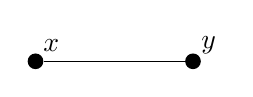
\begin{tikzpicture}
                    \node (labx) at (0.2,0.2) {$x$};
                    \node (laby) at (2.2,0.2) {$y$};
                    \node (x) at (0,0) [circle,fill,inner sep=2pt] {};
                    \node (y) at (2,0) [circle,fill,inner sep=2pt] {};
                    \draw (x) -- (y);
                \end{tikzpicture}
            \end{gather*}
        \item Interaction vertex\footnote{Four legs were drawn as an example, but this can be generalized to any order of interaction term.} $-i\lambda\int d^4z$:
            \begin{gather*}
                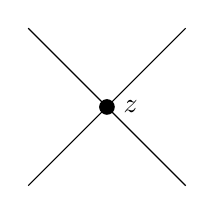
\begin{tikzpicture}
                    \node (z) at (0.3,0) {$z$};
                    \node (x) at (0,0) [circle,fill,inner sep=2pt] {};
                    \draw (-1,-1) -- (1,1);
                    \draw (-1,1) -- (1,-1);
                \end{tikzpicture}
            \end{gather*}
    \end{itemize}
    The main idea of these rules is to draw all possible diagrams consistent with the given interaction Lagrangian and translate them into analytic expressions. However, to obtain the correct normalization we should take the following remark into account:
    \begin{remark}
        Symmetry factors of diagrams should be accounted for in analytic expressions. As an example consider the following vacuum bubble:
        \begin{gather*}
            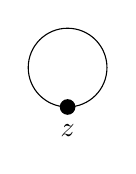
\begin{tikzpicture}
                \node (z) at (0,-0.3) {$z$};
                \node (x) at (0,0) [circle,fill,inner sep=2pt] {};
                \draw (0,0.5) circle (0.5);
            \end{tikzpicture}
        \end{gather*}
        This diagram has \textbf{symmetry factor} 2 (one can interchange the two legs) and hence this diagram gives the analytic expression $-\frac{i\lambda}{2}\int d^4zD_F(z-z)$.
    \end{remark}
\chapter{Gauge Theory}\label{chapter:gauge_theory}

    Using the tools of differential geometry, as presented in chapter \ref{chapter:bundles} and onwards, we can introduce the general formulation of gauge theories and in particular Yang-Mills theories. Valuable references for these subjects are \cite{principal_bundles,sen_nash,schuller,gauge1}.

\section{Gauge invariance}

    Consider a general Lie group\footnote{This group is often called the \textbf{gauge group} in the physics literature.} $G$, acting on a Hilbert bundle\footnote{As explained in chapter \ref{chapter:classical_fields} this bundle is in general obtained as an associated bundle of the frame bundle (or a reduction thereof), possibly tensored with another bundle when we want extra symmetries.} $\mathcal{H}$ of physical states over a base manifold $M$. A general gauge transformation has the form
    \begin{gather}
        \label{qft:gauge_transformation}
        \psi'(x) = U(x)\psi(x)
    \end{gather}
    where $\psi, \psi':M\rightarrow\mathcal{H}$ are sections of the physical Hilbert bundle and $U:M\rightarrow G$ encodes the local behaviour of the gauge transformation ($U$ is assumed to be a unitary representation with respect to the Hilbert structure on $\mathcal{H}$). As such a gauge transformation constitutes a vertical automorphism of the Hilbert bundle.

    \begin{axiom}[Local gauge principle]
        The Lagrangian functional $\mathcal{L}[\psi]$ is invariant under the action of the gauge group $G$:
        \begin{gather}
            \mathcal{L}[U\psi] = \mathcal{L}[\psi].
        \end{gather}
    \end{axiom}

    Generally this gauge invariance can be achieved in the following way. Denote the Lie algebra corresponding to $G$ by $\mathfrak{g}$. Because the gauge transformation is local, the information on how it varies from point to point should be able to propagate through space. This is done by introducing a new field $B_\mu(x)$, called the \textbf{gauge field}. The most elegant formulation uses the concept of covariant derivatives:
    \newdef{Covariant derivative}{\index{covariant!derivative}\index{minimal!coupling}
        When gauging a certain symmetry group one replaces the ordinary partial derivatives by the following covariant derivative (this is called \textbf{minimal coupling}):
        \begin{gather}
            \mathcal{D}_\mu = \partial_\mu + igB_\mu(x)
        \end{gather}
        where $B_\mu:M\rightarrow\mathfrak{g}$ is a new field with values in the Lie algebra of the gauge group. Here we should also note that the explicit action of the covariant derivative depends on the chosen representation of $\mathfrak{g}$ on $\mathcal{H}$. Furthermore, one should pay attention to the fact that we used the physics convention where one multiplies\footnote{The imaginary unit turns anti-Hermitian fields into Hermitian fields.} the gauge field $B$ by a factor $ig$.
    }

    So to achieve gauge invariance one should replace all derivatives by the covariant derivative. However, for this to be a well-defined operation, one should check that the covariant derivative itself satisfies the local gauge principle, i.e. $\mathcal{D}'\psi' = U\mathcal{D}\psi$ (from here on we will suppress the coordinate dependence of all fields):
    \begin{align}
        U^{-1}\left(\pderiv{}{x^\mu} + igB_\mu'\right)\psi' &= U^{-1}\left(\pderiv{}{x^\mu} + igB_\mu'\right)U\psi\nonumber\\
        &= U^{-1}\pderiv{U}{x^\mu}\psi + \pderiv{\psi}{x^\mu} + igU^{-1}B_\mu'U\psi.
    \end{align}
    This expression can only be equal to $\mathcal{D}\psi$ if
    \begin{gather}
        igB_\mu = U^{-1}\pderiv{U}{x^\mu} + igU^{-1}B_\mu'U
    \end{gather}
    which can be rewritten as
    \begin{gather}
        B_\mu' = UB_\mu U^{-1} - \frac{1}{ig}(\partial_\mu U)U^{-1}
    \end{gather}
    or in coordinate-independent form as
    \begin{gather}
        \mathbf{B}' = U\mathbf{B}U^{-1} - \frac{1}{ig}dUU^{-1}.
    \end{gather}
    Up to conventions this is exactly the content of equations \ref{diff:prin:local_compatibility} and \ref{diff:prin:mc_pullback} appearing in the study of connections on principal bundles. This should not come as a surprise since the physical fields are sections of associated vector bundles and hence the principal bundle structure lurks in the background. We conclude that adding interactions is mathematically equivalent to coupling the physical manifold to a principal bundle.

    \begin{example}[QED]
        For quantum electrodynamics, which has U$(1)\cong S^1$ as its gauge group, we use the parametrization $U(x) = e^{ie\chi(x)}$ where $\chi:\mathbb{R}^n\rightarrow\mathbb{R}$. By minimal coupling we obtain
        \begin{align}
            \partial_\mu &\longrightarrow \mathcal{D}_\mu = \partial_\mu + ieA_\mu\\
            A_\mu &\longrightarrow A_\mu' = A_\mu - \partial_\mu\chi
        \end{align}
        where $A_\mu$ is the classic electromagnetic potential. These are indeed the formulas that we introduced in chapter \ref{chapter:maxwell}.
    \end{example}

\section{Spontaneous symmetry breaking}

    \begin{theorem}[Goldstone]\index{Goldstone bosons}
        Consider a QFT with Lie group $G$. Denote the generators of the corresponding Lie algebra by $\mathbf{X}_a$. Generators that do not destroy the vacuum\footnote{This corresponds to a transformation that leaves the vacuum invariant.}, i.e. $\mathbf{X}_av\neq0$, correspond to massless scalar particles.
    \end{theorem}
    The massless bosons from this theorem are called \textbf{Goldstone bosons}.

    ?? COMPLETE ??
\chapter{Quantum Chromodynamics}

	\newprop{OZI rule\footnotemark}{\index{OZI rule}
		\footnotetext{\textit{Okubo, Zweig and Iizuka}}
        \nomenclature[A_OZI]{OZI}{Okubo-Zweig-Iizuka}
		Decay processes for which the corresponding Feynman diagrams become disconnected (initial states and final states are disconnected) when removing internal gluon lines, are suppressed with respect to other processes.
	}

\chapter{Conformal Field Theory}\index{conformal|seealso{CFT}}\label{chapter:CFT}\nomenclature[A_CFT]{CFT}{conformal field theory}

    References for this chapter are \cite{CFT} and the lecture notes by \textit{Schellekens}. For an introduction to Riemannian and conformal geometry, see chapter \ref{chapter:riemann}.

    \begin{property}[Stress-energy tensor]
        Let us consider a theory that is invariant under conformal transformations. The generator of general coordinate transformations is the stress-energy tensor $T$ (the associated current is $\mathcal{J}_\mu = T_{\mu\nu}\varepsilon^\nu$). Requiring conformal invariance then leads to the stress-energy tensor being traceless:
        \begin{gather}
            T^\mu_{\ \mu} = 0.
        \end{gather}
    \end{property}

\section{\texorpdfstring{In dimension $d=2$}{In dimension d=2}}

    In dimension 2 (in Euclidean signature) something special happens. By inserting $d=2$ in the conformal Killing equation we obtain the Cauchy-Riemann equations. The scale factor can thus be written as
    \begin{gather}
        \Omega(x) = \left|\frac{\partial f}{\partial z}\right|^2
    \end{gather}
    for some analytic function $f(z)$. Because of this\footnote{and because we in general look at conformal compactifications (see below)} we will from here one always work in complex coordinates. Switching to complex coordinates also has important consequences for the metric and stress-energy tensor:
    \begin{align}
        g_{zz} = g_{\zbar\zbar} = 0&\qquad g_{z\zbar} = \frac{1}{2}\\
        \partial_zT_{\zbar\zbar} = \partial_{\zbar} T_{zz} = 0&\qquad T_{z\zbar} = 0.
    \end{align}
    The stress-energy tensor thus contains a meromorphic\footnote{The literature often just calls this holomorphic.} component $T_{zz}\equiv T(z)$ and an anti-meromorphic component $T_{\zbar\zbar}\equiv\overline{T}(\zbar)$.

    \newdef{Witt algebra}{\index{Witt algebra}\label{cft:witt_algebra}
        Infinitesimally this gives us an infinite-dimensional algebra. As generators\footnote{These generate the transformation $z\mapsto z-z^{n+1}$ and $\zbar\mapsto\zbar-\zbar^{n+1}$ respectively.} we choose
        \begin{align}
            l_n(z) &:= -z^{n+1}\partial_z\\
            \overline{l}_n(\zbar)&:=-\zbar^{n+1}\partial_{\zbar}.
        \end{align}
        These differential oeprators generate isomorphic Lie algebras with the following commutation relation:
        \begin{gather}
            [l_m, l_n] = (m-n)l_{m+n}.
        \end{gather}
        This Lie algebra is called the \textbf{Witt algebra}.
    }

    \begin{remark}
        Often one finds in the literature that the conformal group of a 2D CFT is infinite-dimensional. However, this statement is not entirely true. It is true that the Witt algebra is infinite-dimensional, but one cannot globally exponentiate all generators $l_m$. First of all it should be remarked that the space of all holomorphic functions does not even have a group structure because the composition of holomorphic functions does not have to be holomorphic. The correct conformal group for 2D Euclidean CFT's is the M\"obius group $\text{PSL}(2, \mathbb{C})$. This group is obtained as the Lie group generated by $l_0$ and $l_{\pm1}$ (the only generators that can be exponentiated globally).

        What is true is that the conformal group of 2D Minkowski space is infinite-dimensional. It can be shown that $\text{Conf}(\mathbb{R}^{1, 1})$ is isomorphic to $\text{Diff}(S^1)_+\times\text{Diff}(S^1)_+$ where the (orientation-preserving) diffeomorphism group Diff$(S^1)_+$ is indeed an infinite-dimensional Lie group (see the intermezzo further below).

        At last we should comment that although the conformal group of $\mathbb{R}^{2, 0}$ is finite-dimensional, the infinite-dimensionality of the Witt algebra (and of its extensions) is sufficient for all physical purposes. The algebraic constraints turn this theory into an integrable theory and allow us to solve it exactly.
    \end{remark}

    \newdef{Primary field}{\index{primary!field}\index{conformal!weight}
        A quasi-primary field is defined as any field that transforms tensorially under global conformal transformations:
        \begin{gather}
            \phi'(z', \zbar') = \left(\pderiv{f}{z}\right)^h\left(\pderiv{f}{\zbar}\right)^{\overline{h}}\phi(f(z), \overline{f}(\zbar))..
        \end{gather}
        Fields that satisfy this relation for all conformal transformations are called primary fields. The tuple $(h, \overline{h})$ is called the \textbf{conformal weight} of the field.
    }

\subsection{\difficult{Intermezzo: Minkowski space}}

    As mentioned in the remark above, the conformal group of 2D Minkowski space is infinite-dimensional. The theory of infinite-dimensional manifolds is however a bit more intricate than the theory of finite-dimensional manifolds. A little introduction is therefore in order. ?? MOVE THIS TO CHAPTER ''INFINITE'' ??

    \newdef{Fr\'echet manifold}{
        A Fr\'echet manifold is a Hausdorff space $M$ together with an atlas of coordinate charts $(U, \varphi)$ such that $\varphi:U\rightarrow F_U$ are homeomorphisms onto a Fr\'echet space and such that the transition functions are smooth maps (of Fr\'echet spaces).
    }

    Using the above definitions we can start to analyze the group Diff$(S^1)_+$. First of all we look at the space of all smooth maps $S^1\rightarrow S^1$. This space has the structure of a Fr\'echet manifold modelled on the Fr\'echet space $\mathfrak{X}(S^1)$ of vector fields on the circle\footnote{By this definition we see that $\mathfrak{X}(S^1)$ is isomorphic (as a Lie algebra) to the mapping space $C^\infty(S^1, \mathbb{R})$. Henceforth we identify vector fields $v$ with their corresponding function $\xi$.}:
    \begin{gather}
        \mathfrak{X}(S^1) = \left\{\xi(\theta)\frac{\partial}{\partial\theta}:\theta\in C^\infty(S^1)\right\}.
    \end{gather}
    Let $V_0$ be the set of vector fields which have norm $||v||\leq\pi$ and let $U_0$ be the set of smooth mappings $f\in C^\infty(S^1, S^1)$ such that $f(\theta)\neq-\theta$ for all $\theta\in S^1$. Then there exists a diffeomorphism $\psi:V_0\rightarrow U_0$ which assigns to any vector field $v$ the function $\psi_v:S^1\rightarrow S^1$ such that the arc between $\theta$ and $\psi_v(\theta)$ has length $||v(\theta)||$. If we choose an open subset $U\subset U_0$ of diffeomorphisms then we obtain a chart $(U, \psi^{-1})$ around the identity map. Charts around any diffeomorphism $f:S^1\rightarrow S^1$ are obtained by left multiplication of $U$.

    The Lie algebra of Diff$(S^1)_+$ is accordingly given by $\mathfrak{X}(S^1)$ but the induced Lie bracket is the commutator of vector fields with the opposite sign: \[[\cdot, \cdot]_{Lie} = -[\cdot, \cdot]_{\mathfrak{X}(S^1)}.\] Now it is interesting to note that the Witt algebra is actually a subalgebra of $\mathfrak{X}(S^1)$. Consider the maps $\xi_n(\theta):=-ie^{in\theta}$ (the minus sign is a convention). The associated vector fields then satisfy
    \begin{gather}
        \left[\xi_k(\theta)\frac{\partial}{\partial\theta}, \xi_l(\theta)\frac{\partial}{\partial\theta}\right] = -i(l-k)\xi_{k+l}(\theta)\frac{\partial}{\partial\theta}.
    \end{gather}
    These are exactly the relations for the Witt algebra.

\section{Quantization}

    \sremark{From here one we will always work in 2 dimensions.}

\subsection{Radial quantization}

    The charge of a conserved current $\mathcal{J}^\mu$ is generally given by the following formula\footnote{See Noether's theorem \ref{qft:noethers_theorem}.}:
    \begin{gather}
        Q = \int_\Sigma\mathcal{J}^0(x, t)
    \end{gather}
    where $\Sigma$ is a spacelike hypersurface. Often we will compactify the spatial dimension (this can be seen as some kind of regularization) and Wick rotate the time dimension. By a conformal transformation one can then go back to the plane (mapping one end of the cylinder to the origin and the other side to a circle at $+\infty$). After these transformations we obtain the following form for an operator on the plane:
    \begin{gather}
        Q_\varepsilon = \frac{1}{2\pi i}\oint dz\varepsilon(z)T(z) + \frac{1}{2\pi i}\oint d\zbar\varepsilon(\zbar)\overline{T}(\zbar).
    \end{gather}
    As usual we expect an infinitesimal transformation of a field $\phi$ to be given by the commutator $[Q_\varepsilon, \phi(w, \overline{w})]$ or in integral form by\footnote{We implicitly assumed a holomorphic split such that we can ignore (antiholomorphic) $\overline{T}(\zbar)$ contributions.} \[\frac{1}{2\pi i}\oint dz\varepsilon(z)[T(z)\phi(w, \overline{w}) - \phi(w, \overline{w})T(z)].\] However, because all the objects in this formula are operators we should take into account the operator ordering. On the plane this is given by the so-called \textbf{radial ordering}:\index{radial ordering}
    \begin{gather}
        \mathcal{R}(A(z, \zbar)B(w, \overline{w})) =
        \begin{cases}
            A(z, \zbar)B(w, \overline{w})&|z|>|w|\\
            B(w, \overline{w})A(z, \zbar)&|w|>|z|.
        \end{cases}
    \end{gather}
    After a deformation of the integration contour we obtain the following general formula:
    \begin{gather}
        [Q_\varepsilon, \phi(w, \overline{w})] = \frac{1}{2\pi i}\oint dz\varepsilon(z)\mathcal{R}(T(z)\phi(w, \overline{w}))
    \end{gather}
    where the contour is now a circle around the point $w$. For primary fields with conformal weight $h$ one can also write an infinitesimal transformation as \[\delta_\varepsilon\phi(z, \zbar) = h(\partial_z\varepsilon(z))\phi(z, \zbar) + \partial_z\phi(z, \zbar).\] Comparing these two expressions leads us to the following form of the operator product:
    \begin{gather}
        \mathcal{R}(T(z)\phi(w, \overline{w})) = \frac{h}{(z-w)^2}\phi(w, \overline{w}) + \frac{1}{z-w}\partial_w\phi(w, \overline{w}) + \text{higher order in } (z-w)
    \end{gather}
    An expression of this form is called an \textbf{operator product expansion} (OPE).\nomenclature[A_OPE]{OPE}{operator product expansion}

\subsection{Virasoro algebra}\index{Virasoro algebra}

    When going from classical systems to quantum systems we have to replace symmetry actions by (unitary) projective representations. As in the case of ordinary groups, the projective representations of Lie groups are related to central extensions. As an example of the Lie group-Lie algebra correspondence it can be shown that central extensions of Lie algebras (see section \ref{section:central_extension_algebra}) are in correspondence with central extensions of Lie groups.

    If we now want a quantum theory equipped with an action of the conformal group, then we need to construct a central extension of the Witt algebra. By applying the construction of section \ref{section:central_extension_algebra} we obtain the \textbf{Virasoro algebra} as a (universal) central extension of the Witt algebra by\footnote{The reason why we extend by $\mathbb{C}$ instead of $\mathbb{R}$ is that we are working with complexified Lie algebras.} $\mathbb{C}$ associated to the cocycle
    \begin{gather}
        \Theta:(L_m, L_n)\mapsto\frac{c}{12}m(m^2-1)\delta_{m+n, 0}.
    \end{gather}

    To obtain the Virasoro algebra from a more physical point of view we look at the stress-energy tensor. If we choose the current $\mathcal{J}^n(z) := z^{n+1}T(z)$, we expect to obtain the transformation $z\longrightarrow z-z^{n+1}$. In analogy with the generators of the Witt algebra (definition \ref{cft:witt_algebra}) we call this generator $L_n$:
    \begin{gather}
        L_n := \frac{1}{2\pi i}\oint dzz^{n+1}T(z).
    \end{gather}
    This relation can be inverted using the residue theorem to obtain the following expression for (the holomorphic component of) the stress-energy tensor:
    \begin{gather}
        T(z) = \sum_{n\in\mathbb{Z}}z^{-n-2}L_n.
    \end{gather}
    Using the above expression and the product operator expansion of $T(z)T(w)$ one obtains exactly the commutation relations of the Virasoro algebra:
    \begin{gather}
        [L_m, L_n] = (m-n)L_{m+n} + \frac{c}{12}m(m^2-1)\delta_{m+n, 0}.
    \end{gather}
    The occurrence of the central charge $c$ gives a conformal anomaly on quantization (see the definition of the vacuum further below). However, the central charge does not affect the $\mathfrak{sl}(2, \mathbb{C})$ subalgebra spanned by $L_{-1}, L_0$ and $L_1$. This implies that concepts such as the conformal weight are still useful.

\subsection{Representation theory}

    \newdef{Highest weight state}{
        A state with minimal eigenvalue for $L_0$. Equivalently, a state that is annihilated by all generators $L_n$ for $n\geq1$:
        \begin{gather}
            L_n|h\rangle = 0.
        \end{gather}
    }

    \newdef{Vacuum}{\index{vacuum}
        Consider the Virasoro generators $\{L_n\}_{n\in\mathbb{Z}}$. The vacuum $|0\rangle$ is defined as the maximally symmetric state. In terms of generators this means that \[L_n|0\rangle = 0\] for as many $n\in\mathbb{Z}$ as possible. However, due to the Virasoro commutation relations (and in particular the central charge) this is not possible for all $n\in\mathbb{Z}$. Instead one can only require that this expression vanishes for all $n\geq-1$.
    }

    \newdef{Descendants}{
        By acting with the generators $L_n$, where $n\leq-1$, on a highest weight state $|h\rangle$ one obtains a whole family of states. These are called the descendants of $|h\rangle$ and together they span the Verma module\footnote{See definition \ref{lie:verma_module}.} (associated to $|h\rangle$).
    }
\chapter{Supersymmetry}

    For an introduction to superstructures in algebra, see section \ref{section:graded_spaces}.

\section{Extensions of the Standard Model}

    \begin{theorem}[Coleman-Mandula]\index{Coleman-Mandula}
        Consider a quantum field theory with the following constraints:
        \begin{enumerate}
            \item There exists a mass gap.
            \item For every mass $M$ there exist only finitely many particle species with mass $\leq M$.
            \item The two-point scattering amplitudes are nonvanishing for almost every energy.
            \item The (two-point) scattering amplitudes are analytic in the particle momenta.
        \end{enumerate}
        If the symmetry group (of the $S$-matrix) contains a subgroup isomorphic to the Poincar\'e group\footnote{To be precise: its universal cover.}, then it can be written as the direct product of the Poincar\'e group and an internal gauge group.
    \end{theorem}
    \sremark{In other words, it is impossible to combine the Poincar\'e group in a nontrivial way with the internal symmetry group.}

    Now the question arises if one can do better, i.e. is there a nontrivial way to extend this total symmetry group. A first possibility was given by conformal field theories in chapter \ref{chapter:CFT}. CFT's do not admit an $S$-matrix and hence the above theorem is clearly not applicable. However, a second and more intricate possibility is given by supersymmetry. Here one does not work with an ordinary symmetry Lie algebra\footnote{See the original paper \cite{coleman_mandula} for why exactly the algebra plays an essential role.} but with a Lie superalgebra. By allowing superspaces, or equivalently fermionic symmetry generators, one can generalize the Coleman-Mandula theorem. The resulting generalization was proven by \textit{Sohnius, Lopusza\'nski} and \textit{Haag}.
\chapter{Entanglement in QFT}

    This chapter should be seen as a generalization of the content (in particular the characterization and computation of entanglement) in chapter \ref{chapter:quantum_computing} to the continuum setting. The main reference is \cite{entanglement_entropy, tuybens}.

\section{Lattice theories}

    In this section we remind the reader of the most important definitions and constructions in ordinary quantum information theory by applying it to a lattice theory. Taking the lattice spacing to zero will then let us extend the definitions to continuum field theories (up to some technicalities that we will explain when necessary). For simplicity we will assume that the local Hilbert space is finite-dimensional.

    Consider a bipartite subdivision $A\cup A^c$ of the lattice, given by a codimension-1 hypersurface $\partial A$ (called the \textbf{entangling surface}).\index{entangling surface} This induces a binary factorization of the total Hilbert space (we assume that all degrees of freedom are confined to individual vertices) and hence we can compute the reduced density matrix for either ($A$ or its complement $A^c$). The eigenvalues (which solely depend on the entangling surface $\partial A$) allow us to calculate the von Neumann entropy:\footnote{Certain assumption ought to be made as to keep the entropy finite whenever the state-space is infinite-dimensional since it can be shown that the set of states with infinite von Neumann entropy is trace norm-dense (see \cite{Eisert_entropy}).}
    \begin{gather}
        S(\rho_A) := -\text{tr}(\rho_A\ln\rho_A) = -\sum_i\rho_i\ln\rho_i.
    \end{gather}
    In the same way we can also introduce the R\'enyi $q$-entropy:\index{entropy!R\'enyi}
    \begin{gather}
        S_q(\rho_A) := \frac{1}{1-q}\ln\left(\sum_i\rho_i^q\right).
    \end{gather}
    \begin{property}[Limiting case]
     First of all one can analytically continue the definition of the $q$-entropy to arbitrary positive real numbers. The limit $q\rightarrow1$ coincides with the von Neumann entropy.
    \end{property}


\chapter{\difficult{Axiomatic QFT}}

    For the sections on the Haag-Kastler framework and its extensions we refer to the work of \textit{Brunetti, Fredenhagen et al}, while reference for the remaining sections on algebraic QFT is \cite{baez_aqft}. For the section on TQFTs we refer to the original paper of \textit{Atiyah} \cite{atiyah}.

\section{Algebraic QFT}
\subsection{Haag-Kastler axioms}

    \begin{axiom}[Local net of observables]\index{microcausality|see{locality}}\index{Einstein!causality}\index{locality}\label{qft:microcausality}
        To every causally closed set\footnote{See definition \ref{relativity:causal_closure}.} $O$ one associates a $C^*$-algebra $\mathcal{A}(O)$. We require this assignment to satisfy the following conditions:
        \begin{enumerate}
            \item \textbf{Isotony}: If $O_1\subset O_2$ then $\mathcal{A}(O_1)\hookrightarrow\mathcal{A}(O_2)$.
            \item \textbf{(Causal) locality}\footnote{Also called \textbf{microcausality} or \textbf{Einstein causality}.}: If $O_1$ and $O_2$ are spacelike separated then $[\mathcal{A}(O_1), \mathcal{A}(O_2)] = 0$ (as a graded commutator) within a larger algebra $\mathcal{A}(O)$ such that $O_1, O_2\subset O$.
        \end{enumerate}
    \end{axiom}
    \sremark{The isotony condition implies that local nets of observables are modelled by copresheaves $\mathbf{Mink}\rightarrow\mathbf{C^*Alg}$ that map (mono)morphisms to monomorphisms.}

    \begin{axiom}[Poincar\'e covariance]
        For all causally closed sets $O$ and Poincar\'e transformations $\Lambda$ there exists an isomorphism $\alpha^O_\Lambda:\mathcal{A}(O)\rightarrow\mathcal{A}(\Lambda O)$ such that the following conditions are satisfied:
        \begin{enumerate}
            \item If $O_1\subset O_2$ then $\alpha_\Lambda\circ\iota_{O_1,O_2} = \iota_{\Lambda O_1, \Lambda O_2}\circ\alpha_\Lambda$.
            \item The isomorphisms satisfy a composition rule: $\alpha^{\Lambda O}_{\Lambda'}\circ\alpha^O_\Lambda = \alpha^O_{\Lambda'\Lambda}$.
        \end{enumerate}
    \end{axiom}

    \begin{axiom}[Spectrum]
        For all spacetime regions $O$ one can construct a faithful $C^*$-algebra representation $\rho_O$ of $\mathcal{A}(O)$ on a fixed Hilbert space (see the GNS construction \ref{operators:gns}). The different representations should be compatible, i.e. if $O_1\subset O_2$ then the restriction of $\rho_{O_2}$ to $\mathcal{A}(O_1)$ should equal $\rho_{O_1}$. Furthermore, all spacetime translations are to be implemented unitarily:
        \begin{gather}
            U(a)\rho_O(c)U(a)^{-1} = \rho_{O+a}(\alpha^O_a(c))
        \end{gather}
        for all $c\in\mathcal{A}(O)$, where $U$ is a unitary representation of the translation subgroup. In addition we require that the generators of the translation subgroup have a spectrum that is contained in the future light cone.
    \end{axiom}

    The following axiom is not part of the standard Haag-Kastler framework but can be added to introduce a notion of time evolution:
    \begin{axiom}[Time slice]
        Consider two spacetime regions $O_1, O_2$. If $O_1$ contains a Cauchy surface of $O_2$ then the morphism $\mathcal{A}(O_1\hookrightarrow O_2)$ of $C^*$-algebras is an isomorphism.
    \end{axiom}

    \begin{axiom}[Haag duality]\index{Haag!duality}
        Let $\overline{O}$ denote the spacelike complement of $O$ and let $\mathcal{A}'$ denote the commutant of $\mathcal{A}$. Haag duality states that\footnote{Here it should be understood that $\mathcal{A}\left(\overline{O}\right)$ is the algebra generated by all algebras $\mathcal{A}(Q)$ where $Q$ ranges over the causally closed sets in $\overline{O}$.}
        \begin{equation}
            \mathcal{A}\left(\overline{O}\right)' = \mathcal{A}(O)
        \end{equation}
        for all causally closed sets $O$.
    \end{axiom}
    \remark{Haag duality is known to hold for all free theories and even for some interacting theories. However, it is also known to fail in the case of symmetry breaking \cite{Roberts_haag}.}

    To generalize the above axiom system to globally hyperbolic space times, we must enter the realm of category theory. We will follow the notation\footnote{This may cause confusion with other notations used in this text. $\mathbf{Loc}$ here has nothing to do with the category of locales from chapter \ref{chapter:topology}.} of \cite{cal_strobl} (?? AND OTHERS ??): Let $\textbf{Loc}$ be the category of globally hyperbolic space times with orientation- and causal structure-preserving isometries. Let $\textbf{Obs}$ be the category of relevant algebras\footnote{Commutative algebras for classical physics and $C^*$-algebras for quantum theories.} together with suitable algebra morphisms. The assignment of algebras is then given by a functor $\func{\mathfrak{U}}{Loc}{Obs}$. The Haag-Kastler framework is recovered when we restrict $\textbf{Loc}$ to the subcategory of globally hyperbolic subsets of some manifold (with inclusions as morphisms).

\subsection{Weyl systems}

    \newdef{Weyl system}{\index{Weyl!system}
        Let $(L, \omega)$ be a symplectic vector space and let $K$ be a complex vector space. Consider a map $W$ from $L$ to the space of unitary operators on $K$. The pair $(K, W)$ is a Weyl system over $(L, \omega)$ if it satisfies
        \begin{equation}
            W(z)W(z') = e^{\frac{i}{2}\omega(z, z')}W(z+z')
        \end{equation}
        for all $z,z'\in L$.
    }
    \remark{This is a generalization of the canonical commutation relations in their Weyl form. (See definition \ref{qm_formalism:CCR}.)}

    \newdef{Heisenberg system}{\index{Heisenberg!system}
        The generators (which exist by Stone's theorem \ref{operator:stone}) $\phi(z)$ of the maps $t\mapsto W(tz)$ are said to form a Heisenberg system. These operators satisfy the following properties:
        \begin{itemize}
            \item $\lambda\phi(z) = \phi(\lambda z)$ for all $\lambda>0$,
            \item $[\phi(z), \phi(z')] = -i\omega(z, z')$,
            \item $\phi(z+z')$ is the closure\footnote{See definition \ref{operator:closure}.} of $\phi(z)+\phi(z')$.
        \end{itemize}
    }

\section{Topological QFT}

    For convenience we remind the reader of some of the notations that we use. $\mathbf{FinVect}$ will denote the category of finite-dimensional vector spaces over $\mathbb{C}$. $\mathbf{Bord}^d_{d-1}$ will denote the category of $d$-dimensional cobordisms (see definition \ref{manifolds:cobordism}).

\subsection{Atiyah-Segal axioms}

    \begin{axiom}[Atiyah-Segal]\index{Atiyah-Segal}\index{TQFT}
        \nomenclature[A_TQFT]{TQFT}{topological quantum field theory}
        A $d$-dimensional topological quantum field theory (TQFT) is a symmetric monoidal functor $F:\textbf{Bord}_{d-1}^d\rightarrow\textbf{FinVect}$. This means (among other things) that $F$ is a map satisfying the following axioms:
        \begin{enumerate}
            \item \textbf{Normalization}: $F(\emptyset)=\mathbb{C}$.
            \item \textbf{Disjoint union}: $F(M\sqcup M') = F(M)\otimes F(M')$.
            \item \textbf{Composition}: If $N=M\cup M'$, where $\partial M$ and $\partial M'$ have opposite orientations, then \[F(N) = F(M)\circ F(M').\]
            \item \textbf{Invariance}: If $f: M\rightarrow M'$ is a diffeomorphism rel boundary then $F\circ f = F$.
        \end{enumerate}
        In the above conditions $M, M'$ are $d$-dimensional cobordisms between $(d-1)$-dimensional (closed) smooth manifolds.
    \end{axiom}

    \begin{example}[1D]
        In 1D a TQFT functor gives rise to the following correspondence:
        \begin{equation*}
            \begin{array}{l|l}
                \text{Point with orientation } + & \text{Vector space } V\\
                \text{Point with reversed orientation } - & \text{Dual space } V^*\\
                \text{Line between points} & \text{Linear map } f:V\rightarrow V\\
                \text{Cap between $\emptyset$ and points } +, - & \text{Coevaluation } \mathbb{C}\rightarrow V\otimes V^*\\
                \text{Cup between points $-, +$ and }\emptyset & \text{Evaluation } V^*\otimes V\rightarrow\mathbb{C}
            \end{array}
        \end{equation*}
        Essentially this gives us the structure of a (finite-dimensional) vector space and its dual.
    \end{example}

    \begin{example}[2D]
        In 2D one can obtain a similar result by drawing all possible configurations. However, the existence and combination of "pair of pants"-diagrams gives a richer structure. For 2D TQFTs the corresponding object is a (finite-dimensional) commutative and cocommutative Frobenius algebra (see definition \ref{linalgebra:frobenius}).
    \end{example}

    In dimensions 3 and higher the definition above is intractable. To allow the construction to be generalized to higher dimensions one considers the following (extended) definition:
    \newdef{Extended TQFT}{\index{TQFT}
        A $d$-dimensional extended TQFT is a symmetric monoidal functor $F:\textbf{Bord}_1^d\rightarrow\textbf{FinVect}$ satisfying the Atiyah-Segal axioms where the invariance axiom is required only at the highest level of $k$-morphisms.
    }

\subsection{Open-closed TQFT}

    For a complete definition we refer to the original paper \cite{open_closed}.

    In the case of ordinary TQFTs as defined in the previous section one considers cobordisms between closed manifolds, hence the relevant objects in this category are manifolds with boundary. A generalization is obtained by relaxing the constraint on the cobordisms and allowing the notion of manifolds with corners (see section \ref{section:manifold_boundary}). For simplicity we will only consider the case of 2D TQFTs (as in the original definition).

    ?? COMPLETE ??

\part{Statistical Mechanics \& Condensed Matter Physics}
\chapter{Thermodynamics}
\section{General definitions}

    \newdef{System}{\index{system}
        The part of space that is of interest.
    }
    \newdef{Environment}{\index{environment}
        The complement of the system in space. More specifically, this denotes the part of space that has a potential influence on the system.
    }

    \newdef{Thermodynamic coordinate}{\index{coordinate}
        Macroscopical variable that describes the system. These are also called \textbf{state variables}.
    }
    \newdef{Intensive coordinate}{
        Coordinate that does not depend on the system size. The opposite notion is called an \textbf{extensive coordinate}.
    }
    \newdef{Thermodynamic equilibrium}{
        A system is said to be in thermodynamic equilibrium if it is simultaneously in thermal, mechanical and chemical equilibrium. In this case, it is fully described by a set of constant thermodynamic coordinates.
    }
    \begin{property}[Uniformity]
        During thermodynamic equilibrium all intensive coordinates are uniform throughout the system.
    \end{property}

    \newdef{Isolated system}{
        A system that cannot interact with its environment (e.g. due to the presence of impenetrable walls).
    }
    \newdef{Diathermic wall}{\index{wall}
        A wall that only allows heat transfer. This should be distinguished from an \textbf{adiabatic wall}, i.e. a wall that does not allow any transfer of heat.
    }
    \newdef{Heat bath}{\index{bath}\index{reservoir}
        A heat bath or \textbf{thermal reservoir} is a thermodynamic system (often part of the environment) for which the temperature remains constant during the exchange of heat, i.e. it has a virtually infinite heat capacity.
    }
    \newdef{Open system}{\index{open!system}
        A system that is allowed to interact with its environment.
    }
    \newdef{Quasistatic process}{
        A sequence of equilibrium states separated by infinitesimal changes.
    }
    \newdef{Path}{\index{path}
        The sequence of equilibrium states in a thermodynamic process is called its path.
    }

\section{Postulates}

    \begin{axiom}[Zeroth law]
        If two objects are in thermal equilibrium with a third object, they are also in thermal equilibrium with each other.
    \end{axiom}
    \begin{axiom}[First law]
        The change in internal energy is given by
        \begin{gather}
            \label{thermo:first_law}
            \Delta U = Q + W,
        \end{gather}
        or, infinitesimally, by
        \begin{gather}
            \label{thermo:first_law_differential}
            dU = \delta Q + \delta W,
        \end{gather}
        where $W$ denotes the work done on the system and $Q$ denotes the heat that was extracted from the environment.
    \end{axiom}
    \sremark{The $\delta$ in the heat and work differentials implies that these are ``inexact'' differentials, i.e. they are not the differential of functions of the thermodynamic coordinates alone. See Section \ref{section:forms} for more information on differential forms.}

    \begin{axiom}[Kelvin-Planck formulation of the second law]
        No machine can absorb an amount of heat and completely transform it into work.
    \end{axiom}
    \begin{axiom}[Clausius formulation of the second law]
        Heat cannot be passed from a cooler object to a warmer object without performing work.
    \end{axiom}

    \newformula{Clausius's inequality}{\index{Clausius!inequality}
        In differential form the inequality reads as
        \begin{gather}
            \label{thermo:clausius_inequality}
            \frac{\delta Q}{T} \geq 0.
        \end{gather}

        ?? COMPLETE THIS STATEMENT (WHICH INEQUALITY?) ??
    }

    \begin{axiom}[Third law]
        No process can reach absolute zero through a finite sequence of operations.
    \end{axiom}

\section{Gases}
\subsection{Ideal gases}

    \begin{theorem}[Ideal gas law]\index{ideal gas constant}
        \begin{gather}
            \label{thermo:ideal_gas_law}
            PV = nRT,
        \end{gather}
        where $R$ is the \textbf{ideal gas constant} $R\approx8.314 \frac{\mathrm{J}}{\mathrm{K\,mol}}$.
    \end{theorem}
\chapter{Statistical Mechanics}

\section{Axioms}

    \begin{axiom}[Ergodic principle]\index{ergodic!principle}
        All microstates corresponding to the same macrostate are equally probable.
    \end{axiom}

    \begin{axiom}[Boltzmann formula]\index{Boltzmann!entropy}
        The entropy of a system is given by
        \begin{gather}
            \label{statmech:boltzmann_formula}
            S := k\ln\Omega(E,V,N,\alpha),
        \end{gather}
        where $\Omega$ denotes the number of microstates corresponding to the system with energy $E$, volume $V$, number of particles $N$ and any other state variable (these are denoted by $\alpha$). In general $S$ will be the Shannon entropy \ref{prob:shannon_entropy}.
    \end{axiom}

\section{Temperature}

    \begin{formula}\index{temperature}\label{statmech:temperature}
        The temperature of a system in contact with a heat bath is defined as follows:
        \begin{gather}
            T := \left(\pderiv{E}{S}\right)_V.
        \end{gather}
    \end{formula}

\section{Canonical ensemble}

    \newformula{Partition function}{\index{partition!function}\label{statmech:partition_function}
        The partition function for discrete systems is defined as
        \begin{gather}
            Z(T) := \sum_i{g_ie^{-\beta\varepsilon_i}}.
        \end{gather}
        The analogue for continuous systems is
        \begin{gather}
            Z(T) := \int\Omega(E,V,N)e^{-\beta E}dE.
        \end{gather}
    }

    \begin{formula}
        Consider a system of $N$ indistinguishable noninteracting particles. Let $\varepsilon_i$ be the energy associated with the $i^{th}$ energy level and let $g_i$ be its degeneracy. The probability $p_i$ of finding a particle in the $i^{th}$ energy level is given by
        \begin{gather}
            p_i = \frac{g_i e^{-\beta\varepsilon_i}}{Z}.
        \end{gather}
    \end{formula}

    \newdef{Helmholtz free energy}{\index{Helmholtz!free energy}\index{energy}\index{entropy!free}\index{Massieu potential}
        The Helmholtz free energy is defined as follows:
        \begin{gather}
            F := -k_BT\ln Z.
        \end{gather}
        For the canonical ensemble it can be shown that this is equal to a Legendre transformation of the energy: $F= E-TS$.

        One can also obtain the Helmholtz free energy as a different Legendre transform using the ideas of information theory (Chapter \ref{chapter:info}). There it was shown that the convex potentials associated to exponential families were related to the free energy. If Equation \eqref{info:free_energy} is compared to the above one, it can be seen that \[\psi = -\beta F.\] This quantity is sometimes called the \textbf{(Helmholtz) free entropy} or \textbf{Massieu potential} to distinguish it from the (Helmholtz) free energy. It was also shown that the associated dual coordinates are the expectation values, in this case the internal energy (up to a sign), and the dual potential was equal to the (negative) Shannon entropy. Putting this together gives:
        \begin{align*}
            \eta &= \beta\pderiv{\psi}{\beta} - \psi\\
            \overset{\text{def.}}{\iff} -S &= \beta (-U) - (-\beta F)\\
            \iff F &= U - TS_B,
        \end{align*}
        where the relation between the Boltzmann entropy $S_B$ and the Shannon entropy $S$ was used.
    }

\section{Grand canonical ensemble}

    \newformula{Grand canonical partition function}{
        The partition function of the $i^{th}$ energy level is given by
        \begin{gather}
            \mathcal{Z}_i := \sum_{n_k}e^{\beta n_k(\mu - \varepsilon_i)}.
        \end{gather}
        The grand canonical partition function is given by
        \begin{gather}
            \mathcal{Z} := \prod_i\mathcal{Z}_i = \sum_{n_k, \varepsilon_i}e^{\beta n_k(\mu - \varepsilon_i)}.
        \end{gather}
    }
    \remark{In the case of fermions, i.e. $n_i\in\{0,1\}$, this formula reduces to $\mathcal{Z} = e^{\beta\mu}Z$.}

    \newdef{Fugacity}{\index{fugacity}\label{statmech:fugacity}
        \begin{gather}
            z := e^{\mu N}
        \end{gather}
    }

    \begin{formula}[Quantum mechanics]
        For quantum-mechanical systems one can rewrite the partition function as follows:
        \begin{gather}
            \mathcal{Z} = \mathrm{tr}\exp\left(-\frac{\hat{H}-\mu\hat{N}}{T}\right).
        \end{gather}
        This reduces to the above expressions when working in the single-particle eigenbasis (this is only possible for free theories).
    \end{formula}

\section{Energy}

    \begin{theorem}[Virial theorem]\index{virial theorem}\label{statmech:virial_theorem}
        \begin{gather}
            \langle T \rangle = -\frac{1}{2}\sum_k\langle \vector{r}_k\cdot\vector{F}_k \rangle
        \end{gather}
    \end{theorem}
    \begin{result}
        For potentials of the form $V=ar^{-n}$ this becomes
        \begin{gather}
            2\langle T \rangle = -n\langle V \rangle.
        \end{gather}
    \end{result}

    \begin{theorem}[Equipartition theorem]\index{equipartition theorem}
        Let $x$ be a generalized coordinate.
        \begin{gather}
            \left\langle x^k\pderiv{H}{x^l} \right\rangle = k_bT\delta_{kl}
        \end{gather}
    \end{theorem}
    \begin{result}
        For quadratic Hamiltonians this can be rewritten using Euler's theorem for homogeneous functions \ref{calculus:euler_homogeneous_functions}:
        \begin{gather}
            \langle T \rangle = \frac{1}{2}k_bT.
        \end{gather}
    \end{result}

\section{Black-body radiation}

    \begin{formula}[Planck's law]\index{Planck}\label{statmech:plancks_law_frequency}
        \begin{gather}
            B_\nu(\nu,T) = \frac{2h\nu^3}{c^2}\frac{1}{e^{\frac{h\nu}{kt}} - 1}
        \end{gather}
    \end{formula}

    \begin{formula}[Wien's displacement law]\index{Wien}\label{statmech:wiens_displacement_law}
        \begin{gather}
            \lambda_{\max}T = b,
        \end{gather}
        where the constant $b = \num{2,8977729(17)E-3}$ Km is called \textbf{Wien's displacement constant}.
    \end{formula}
\chapter{Material Physics}

\section{Crystals}

    \begin{theorem}[Steno's law]\index{Steno}
        The angles between crystal faces of the same type are constant and do not depend on the total shape of the crystal.
    \end{theorem}

    \newdef{Zone}{\index{zone}
        The collection of faces parallel to a given axis. The axis itself is called the \textbf{zone axis}.
    }

\subsection{Analytic representation}

    \newdef{Miller indices}{\index{index!Miller}
        Let $a, b, c$ be the lengths of the (not necessarily orthogonal) basis vectors of the crystal lattice. The lattice plane intersecting the axes at $\left(\frac{a}{h},\frac{b}{k},\frac{c}{k}\right)$ is denoted by the Miller indices $(h\ k\ l)$.
    }
    \begin{notation}
        Negative numbers are often written as $\overline{a}$ instead of $-a$.
    \end{notation}

    \newformula{Axes}{
        Let $a, b, c$ denote the lengths of the basis vectors. The axis formed by the intersection of the planes $(h_1\ k_1\ l_1)$ and $(h_2\ k_2\ l_2)$ is denoted by $[u\ v\ w]$. Its direction is determined by the point $(au, bv, cw)$ where
        \begin{gather}
            u = \left|
            \begin{array}{cc}
                k_1&l_1\\
                k_2&l_2
            \end{array}\right|
                    \qquad
            v = \left|
            \begin{array}{cc}
                l_1&h_1\\
                l_2&h_2
            \end{array}\right|
            \qquad
            w = \left|
            \begin{array}{cc}
                h_1&k_1\\
                h_2&k_2
            \end{array}\right|.
        \end{gather}
    }

    \begin{theorem}[Hauy's law of rational indices]\index{Hauy}
        The Miller indices of every natural face of a crystal will always have rational proportions.
    \end{theorem}

\section{Symmetries}

    \newdef{Equivalent planes/axes}{
        When applying certain symmetries to a plane or axis, it often happens that we obtain a set of equivalent planes and axes. These equivalence classes are denoted by $\{h\ k\ l\}$ and $\langle h\ k\ l\rangle$ respectively.
    }

    \newprop{Rotational symmetry}{
        Only $1, 2, 3, 4$ and $6$-fold rotational symmetries can occur.
    }

\section{Crystal lattice}

    \begin{formula}
        For an orthogonal crystal lattice, the distance between planes of the family $(h\ k\ l)$ is given by
        \begin{gather}
            \label{maphy:d_hkl}
            d_{hkl} = \stylefrac{1}{\sqrt{\left(\frac{h}{a}\right)^2 + \left(\frac{k}{b}\right)^2 + \left(\frac{l}{c}\right)^2}}.
        \end{gather}
    \end{formula}

\subsection{Bravais lattice}

    \newdef{Bravais lattice}{\index{Bravais lattice}
        A crystal lattice generated by a certain point group symmetry. There are 14 different Bravais lattices in 3 dimensions. These are the only possible ways to place (infinitely) many points in 3D space by applying symmetry operations consistent with the given point group.
    }

    \newdef{Wigner-Seitz cell}{\index{Wigner-Seitz cell}
        The part of space consisting of all points closer to a given lattice point than to any other.
    }

    \begin{theorem}[Neumann's principle]\index{Neumann}
        The symmetry elements of the physical properties of a crystal should at least contain those of the point group of the crystal.
    \end{theorem}

\subsection{Reciprocal lattice}

    \newformula{Reciprocal basis vectors}{\index{reciprocal lattice}
        The reciprocal lattice corresponding to a given Bravais lattice with primitive basis $\{\vector{a},\vector{b},\vector{c}\}$ is defined by the following reciprocal basis vectors:
        \begin{gather}
            \vector{a}^* := 2\pi\stylefrac{\vector{b}\times\vector{c}}{\vector{a}\cdot(\vector{b}\times\vector{c})}.
        \end{gather}
        The vectors $\vector{b}^*$ and $\vector{c}^*$ are obtained by cyclic permutation of $(a,b,c)$. These vectors satisfy the relations
        \begin{gather}
            \begin{aligned}
                \vector{a}\cdot\vector{a}^* &= 2\pi\\
                \vector{b}\cdot\vector{b}^* &= 2\pi\\
                \vector{c}\cdot\vector{c}^* &= 2\pi
            \end{aligned}
        \end{gather}
    }
    \newnot{Reciprocal lattice vector}{
        The reciprocal lattice vector $\vector{r}^*_{hkl}$ is defined as follows:
        \begin{gather}
            \vector{r}^*_{hkl} := h\vector{a}^* + k\vector{b}^* + l\vector{c}^*.
        \end{gather}
    }

    \begin{property}
        The reciprocal lattice vector $\vector{r}^*_{hkl}$ has the following properties:
        \begin{itemize}
            \item $\vector{r}^*_{hkl}$ is perpendicular to the family of planes $(h\ k\ l)$ of the direct lattice, and
            \item $||\vector{r}^*_{hkl}|| = \stylefrac{2\pi n}{d_{hkl}}$.
        \end{itemize}
    \end{property}

\section{Diffraction}\index{diffraction}
\subsection{Constructive interference}

    \newformula{Laue conditions}{\index{Laue!conditions}
        Suppose that an incident beam makes angles $\alpha_0,\beta_0$ and $\gamma_0$ with the lattice axes. A diffracted beam, making angles $\alpha,\beta$ and $\gamma$ with the axes, will be observed if the following conditions are satisfied:
        \begin{gather}
            \begin{aligned}
                a(\cos\alpha - \cos\alpha_0) &= h\lambda\\
                b(\cos\beta - \cos\beta_0) &= k\lambda\\
                c(\cos\gamma - \cos\gamma_0) &= l\lambda
            \end{aligned}
        \end{gather}
        If these conditions have been met, we observe a diffracted beam of order $hkl$.
    }
    \begin{remark}
        Further conditions can be imposed on the angles, such as the Pythagorean formula for orthogonal axes. This has the consequence that the only two possible ways to obtain a diffraction pattern are:
        \begin{itemize}
            \item a fixed crystal and a polychromatic beam, or
            \item a rotating crystal and a monochromatic beam.
        \end{itemize}
    \end{remark}

    \newformula{Vectorial Laue conditions}{
        Let $\vector{k}_0, \vector{k}$ denote the wave vectors of the incident and diffracted beams respectively. The Laue conditions can be reformulated in the following way:
        \begin{gather}
            \label{maphy:vectorial_laue_condition}
            \vector{k} - \vector{k}_0 = \vector{r}^*_{hkl}.
        \end{gather}
    }

    \newformula{Bragg's law}{\index{Bragg}
        Another equivalent formulation of the Laue conditions is given by the following formula:
        \begin{gather}
            \label{maphy:braggs_law}
            2d_{hkl}\sin\theta = n\lambda
        \end{gather}
        where
        \begin{itemize}
            \item $\lambda$ is the wavelength of the incoming beam,
            \item $\theta$ is the \textbf{Bragg angle}, and
            \item $d_{hkl}$ is the distance between neighbouring planes.
        \end{itemize}
    }
    \begin{remark}
        The angle between the incident and diffracted beams is $2\theta$.
    \end{remark}

    \begin{construct}[Ewald sphere]\index{Ewald sphere}
        A simple construction to determine if Bragg diffraction will occur is the Ewald sphere: Put the origin of the reciprocal lattice at the tip of the incident wave vector $\vector{k}_i$. Construct a sphere with radius $\frac{2\pi}{\lambda}$ centred on the start of $\vector{k}_i$. All points on the sphere that coincide with a reciprocal lattice point satisfy the vectorial Laue condition \ref{maphy:vectorial_laue_condition}. Therefore Bragg diffraction will occur in the direction of all the intersections of the Ewald sphere and the reciprocal lattice.
    \end{construct}

\subsection{Intensity of diffracted beams}

    \newdef{Systematic extinctions}{\index{extinction}
        Every particle in the motive emits its own waves. These waves will interfere and some will cancel out. This leads to the absence of certain diffraction spots. These absences are called systematic extinctions.
    }

    \newdef{Atomic scattering factor}{\index{scattering!factor}
        The waves produced by the individual electrons of an atom, which can have a different phase, can be combined into a resulting wave. The amplitude of this wave is called the atomic scattering factor.
    }
    \newdef{Structure factor}{\index{structure!factor}
        The waves coming from the individual atoms in the motive can also be combined into a resulting wave (again taking into account the different phases). The amplitude of this wave is called the structure factor and it is given by
        \begin{gather}
            \label{maphy:structure_factor}
            F(hkl) = \sum_j\ f_j\exp\big[2\pi i(hx_j + ky_j + lz_j)\big]
        \end{gather}
        where $f_j$ is the atomic scattering factor of the $j^{th}$ atom in the motive.
    }

    \begin{example}
        A useful example  of systematic extinctions is the structure factor of an FCC or BCC lattice for the following specific situations: If $h+k+l$ is odd, $F(hkl) = 0$ for a BCC lattice. If $h,k$ and $l$ are not all even or all odd, $F(hkl) = 0$ for an FCC lattice.
    \end{example}

    \newdef{Laue indices}{\index{Laue!indices}
        Higher order diffractions can be rewritten as a first order diffraction in the following way:
        \begin{gather}
            2d_{nhnknl}\sin\theta = \lambda\qquad\text{with}\qquad d_{nhnknl} = \stylefrac{d_{hkl}}{n}.
        \end{gather}
        Following from the interpretation of the Bragg law as diffraction being a reflection in the lattice plane $(h\ k\ l)$, we can introduce the (fictitious) plane with indices $(nh\ nk\ nl)$. These indices are called Laue indices.
    }
    \sremark{In contrast to Miller indices which cannot possess common factors, the Laue indices obviously can.}

\section{Alloys}

    \begin{property}[Hume-Rothery conditions]\index{Hume-Rothery conditions}
        An element can be dissolved in a metal (forming a solid solution) if the following conditions are met:
        \begin{itemize}
            \item The difference between the atomic radii is $\leq 15\%$.
            \item The crystal structures are the same.
            \item The elements have a similar electronegativity.
            \item The valence is the same.
        \end{itemize}
    \end{property}

\section{Lattice defects}

    \newdef{Interstitial}{\index{interstitial}
        An atom placed at a position which is not a lattice point.
    }

    \newdef{Vacancy}{\index{vacancy|see{Schottky defect}}\index{Schottky!defect}
        A lattice point where an atom is missing. This is also called a \textbf{Schottky defect}.
    }
    \begin{formula}[Concentration of Schottky defects $\dag$]\label{maphy:schottky_defects}
        Let $N, n$ denote the number of lattice points and vacancies respectively. The following relation gives the temperature dependence of Schottky defects:
        \begin{gather}
            \frac{n}{n + N} = e^{-E_v/kT}
        \end{gather}
        where $T$ denotes the temperature and $E_v$ the energy needed to create a vacancy.
    \end{formula}
    \sremark{A similar relation holds for interstitials.}

    \newdef{Frenkel pair}{\index{Frenkel pair}
        An atom displaced from a lattice point to an interstitial location (thereby creating a vacancy-interstitial pair).
    }
    \begin{formula}[Concentration of Frenkel pairs]
        Let $n_i$ denote the number of atoms displaced from the bulk of the lattice to any of $N_i$ possible interstitial positions and thereby creating $n_i$ vacancies. The following relation holds:
        \begin{gather}
            \stylefrac{n_i}{\sqrt{NN_i}} = e^{-E_{fr}/2kT}
        \end{gather}
        where $E_{fr}$ denotes the energy needed to create a Frenkel pair.
    \end{formula}

    \remark{In compounds, the number of vacancies can be much higher than in mono-atomic lattices.}
    \remark{The existence of these defects creates the possibility of diffusion.}

\section{Electrical properties}
\subsection{Charge carriers}

    \newformula{Conductivity}{\index{conductivity}\label{maphy:conductivity}
        Definition \ref{em:conductivity} can be modified to account for both positive and negative charge carriers:
        \begin{gather}
            \sigma := n_nq_n\mu_n + n_pq_p\mu_p.
        \end{gather}
    }
    \sremark{The difference between the concentration of positive and negative charge carriers can differ by orders of magnitude (up to 20) across different materials.}

\subsection{Band structure}

    \newdef{Valence band}{\index{valence band}
        The energy band corresponding to the outermost (partially) filled atomic orbital.
    }
    \newdef{Conduction band}{\index{conduction band}
        The first unfilled energy band.
    }
    \newdef{Band gap}{\index{band gap}
        The energy difference between the valence and conduction bands (if they do not overlap). It is the energy zone where no electron states can exist.\footnote{For a basic derivation see \cite{bransden}.}
    }

    \newdef{Fermi level}{\index{Fermi!level}
        The energy level having a 50\% chance of being occupied at thermodynamic equilibrium.
    }
    \newformula{Fermi function}{\index{Fermi!function}
        The following distribution gives the probability of a state with energy $E_i$ being occupied by an electron:
        \begin{gather}
            \label{maphy:fermi_function}
            f(E_i) = \stylefrac{1}{e^{(E_i - E_f)/kT} + 1}
        \end{gather}
        where $E_f$ is the Fermi level as defined above.
    }

    \begin{formula}
        Let $n$ denote the charge carrier density as before. We find the following temperature dependence:
        \begin{gather}
            n \propto e^{-E_g/2kt}
        \end{gather}
        where $E_g$ is the band gap. This formula can be directly derived from the Fermi function by noting that for intrinsic semiconductors the Fermi level sits in the middle of the band gap, i.e. $E_c - E_f = E_g / 2$, and that for most semiconductors $E_g\gg kT$.
    \end{formula}

    \newdef{Doping}{
        Intentionally introducing impurities to modify the (electrical) properties.
    }
    \newdef{Acceptor}{
        A group-III element added to create an excess of holes in the valence band. The resulting semiconductor is called a \textbf{p-type semiconductor}.
    }
    \newdef{Donor}{
        A group-IV element added to create an excess of electrons in the valence band. The resulting semiconductor is called an \textbf{n-type semiconductor}.
    }

\subsection{Ferroelectricity}

    Some materials can exhibit certain phase transitions between a para-electric and ferroelectric state.

    Para-electric materials have the property that the polarisation $\vector{P}$ and the electric field $\vector{E}$ are proportional. Ferroelectric materials have the property that they exhibit permanent polarization, even in the absence of an electric field. This permanent behaviour is the result of symmetry breaking: The ions in the lattice have been shifted out of their ''central'' positions, which induces a permanent dipole moment.

    The temperature at which this phase transition occurs is called the \textbf{ferroelectric Curie temperature}. Above this temperature the material will behave as a para-electric material.

   \begin{remark}
       Ferroelectricity can only occur in crystals with unit cells that do not have a center of symmetry. This would rule out the possibility of having the asymmetry needed for the dipole moment.
   \end{remark}

    \newdef{Saturation polarization}{\index{polarization}
        The maximum polarization obtained by a ferroelectric material. It it obtained when the \textit{domain formation} reaches a maximum.
    }
    \newdef{Remanent polarization}{
        The residual polarization of the material when the external electric field is turned off.
    }
    \newdef{Coercive field}{
        The electric field needed to cancel out the \textit{remanent} polarization.
    }

    \newdef{Piezoelectricity}{\index{piezoelectricity}
        Materials that obtain a polarization when exposed to mechanical stress are called piezoelectric materials.
    }
    \begin{remark}
        All ferroelectric materials are piezoelectric, but the converse is not true. Moreover, all crystals without a center of symmetry are piezoelectric. This property is however only a necessary (and not a sufficient) condition for ferroelectricity, as mentioned above.
    \end{remark}

    \begin{example}[Transducer]\index{transducer}
        A device that converts electrical energy to mechanical energy (and vice versa).
    \end{example}

\section{Magnetic properties}

    \begin{definition}[Diamagnetism]
        In diamagnetic materials, the magnetization is oriented oppositely to the applied field, so $B < H$. The susceptibility is small, negative and independent of the temperature.
    \end{definition}
    \begin{remark}
        All materials exhibit diamagnetic behaviour.
    \end{remark}

    \begin{definition}[Paramagnetism]
        The susceptibility is small, positive and inversely proportional to the temperature.
    \end{definition}

    \begin{definition}[Ferromagnetism]
        Spontaneous magnetization can occur. The susceptibility is large and dependent on the applied field and temperature. Above a certain temperature, the \textbf{ferromagnetic Curie temperature}, the materials will behave as if they were only paramagnetic.
    \end{definition}

\subsection{Paramagnetism}

    \newformula{Curie's law}{\index{Curie}
        If the interactions between the particles can be neglected, we obtain the following law:
        \begin{gather}
            \label{magentism:curies_law}
            \chi = \stylefrac{C}{T}.
        \end{gather}
        Materials that satisfy this law are called \textbf{ideal paramagnetics}.
    }
    \newformula{Curie-Weiss law}{\index{Weiss|see{Curie-Weiss}}\index{Curie-Weiss}
        If the interactions between particles cannot be neglected, we obtain the a slight correction to Curie's law:
        \begin{gather}
            \label{magentism:curie_weiss__law}
            \chi = \stylefrac{C}{T-\theta}
        \end{gather}
        where $\theta = CN_W$ with $N_W$ the \textbf{Weiss-constant}. This deviation of Curie's law is due to the intermolecular interactions that induce an internal magnetic field $H_m = N_WM$.
    }

    \begin{formula}[Brillouin function]\index{Brillouin function}
        \begin{gather}
            \label{magnetism:brillouin_function}
            B_J(y) := \stylefrac{2J + 1}{2J}\text{coth}\left(\stylefrac{2J + 1}{2J}y\right) - \stylefrac{1}{2J}\text{coth}\left(\stylefrac{y}{2J}\right)
        \end{gather}
        where $y := \stylefrac{g\mu_BJB}{kT}$.
    \end{formula}

    \begin{remark}
        Because $\coth(y\rightarrow\infty)=1$ we have:
        \begin{gather}
            \label{magnetism:absolute_saturation_magnetization}
            \text{if }T\rightarrow0\quad\text{then}\quad M=Ng\mu_BJB_J(y\rightarrow\infty) = Ng\mu_BJ.
        \end{gather}
        This value is called the \textbf{absolute saturation magnetization}.
    \end{remark}

\subsection{Ferromagnetism}

    Ferromagnetics are materials that have strong internal interactions which lead to large scale (with respect to the lattice constant) parallel ordering of the atomic magnetic (dipole) moments. This leads to the spontaneous magnetization of the material and consequently to a nonzero total dipole moment.

    \sremark{In reality ferromagnetic materials do not always spontaneously possess a magnetic moment in the absence of an external field. When stimulated by a small external field, they will however display a magnetic moment, much larger than paramagnetic materials would.}

    \newdef{Domain}{\index{Weiss!domain}
        The previous remark is explained by the existence of Weiss domains. These are spontaneously magnetized regions in a magnetic material. The total dipole moment is the sum of the moments of the individual domains. If not all the domains have a parallel orientation then the total dipole moment can be 0, a small external field is however sufficient to change the domain orientation and produce a large total magnetization.
    }
    \newdef{Bloch walls}{\index{Bloch!walls}
        A wall between two magnetic domains.
    }

    \newdef{Ferromagnetic Curie temperature}{\index{Curie!ferromagnetic Curie temperature}
        Above this temperature the material loses its ferromagnetic properties and it becomes a paramagnetic material following the Curie-Weiss law.
    }

    \remark{For ferromagnetic (and ferrimagnetic) materials it is impossible to define a magnetic susceptibility as the magnetization is nonzero even in the absence of a magnetic field.\footnote{This can be seen from equation \ref{em:M}: $M = \chi H$. The susceptibility should be infinite.} Above the critical temperature (Curie/N\'eel) it is however possible to define a susceptibility as the materials become paramagnetic in this region.
    }

\subsection{Antiferromagnetism}

    When the domains in a magnetic material have an antiparallel order (whenever this is energetically more favourable) the total dipole moment will be small. If the temperature rises, the thermal agitation however will disturb the orientation of the domains and the magnetic susceptibility will rise.

    \newdef{N\'eel temperature}{\index{N\'eel}
        At the N\'eel temperature, the susceptibility will reach a maximum. Above this temperature $(T>T_N)$ the material will become paramagnetic, satisfying the following formula:
        \begin{gather}
            \chi = \stylefrac{C}{T+\theta}.
        \end{gather}
        This resembles a generalization of the Curie-Weiss law with a negative and therefore a virtual critical temperature.
    }

\subsection{Ferrimagnetism}

    Materials that are not completely ferromagnetic nor antiferromagnetic, due to an unbalance between the sublattices, will have a nonzero dipole moment even in the absence of an external field. The magnitude of this moment will however be smaller than that of a ferromagnetic material. These materials are called ferrimagnetic materials.

    \newformula{N\'eel hyperbola}{
        Above the N\'eel temperature it is possible to define a susceptibility given by
        \begin{gather}
            \stylefrac{1}{\chi} = \stylefrac{T}{C} - \stylefrac{1}{\chi_0} - \stylefrac{\sigma}{T - \theta'}.
        \end{gather}
    }
\chapter{Tensor Networks}

\section{Matrix Product States}
\subsection{Finite-dimensional lattices}

    \newdef{Matrix product state}{\index{MPS}
        Let $\mathcal{H}_n$ be the local Hilbert spaces of dimension $d_n$ where $n\in\{1,\ldots,N\}$. A state $|\psi\rangle$ in the total Hilbert space $\bigotimes_i\mathcal{H}_i$ is a matrix product state (with periodic boundary conditions) if there exist matrices $A^{i_n}(n)\in\mathcal{L}(\mathbb{C}^{D_n}, \mathbb{C}^{D_{n-1}})$ with $i_n\leq d_n$ such that
        \begin{gather}
            |\psi\rangle = \sum_{\{i_k\}}\text{tr}\Big(\prod_n^NA^{i_n}(n)\Big)|i_1\ldots i_N\rangle.
        \end{gather}
        For each lattice site $n$ the set of matrices $\{A^{i_n}_{\alpha\beta}(n)\}$ can be regarded as the content of one rank-3 tensor. The periodic boundary condition requires that $D_0=D_N$ (otherwise the trace would be ill-defined). Different boundary conditions can be implemented by inserting an additional factor $X$ at the end of the trace.
    }
    \begin{notation}
        In the continuation of this chapter we will abbreviate matrix product states as \textbf{MPS}.
    \end{notation}

    \begin{remark}[Physical and virtual spaces]
        For each \textit{physical} index $i_n$ one can regard the matrix $A^{i_n}(n)$ as a linear map between \textit{virtual} (or ancilla) spaces $\mathbb{C}^{D_n}$.
    \end{remark}

    \newformula{MPS projector}{
        Consider an MPS given by tensors $\{A(n)\}_{n\leq N}$. The associated MPS projector is defined as
        \begin{gather}
            \mathcal{P}(A) := \sum_{i, \alpha, \beta}A^i_{\alpha\beta}(n)|i\rangle\langle\alpha\beta|.
        \end{gather}
    }

    \newformula{Transfer operator}{\index{transfer!operator}
        Give the MPS tensors $\{A(n)\}_{n\leq N}$ one can define a transfer operator:
        \begin{gather}
            \label{tennet:transfer_operator}
            \mathbb{E}(n) := \sum_{i=1}^{d_n}A^i(n)\otimes\overline{A^i}(n).
        \end{gather}
    }
    \begin{formula}[Superoperator]\index{super!operator}
        More generally we can define for every local observable $\hat{O}_n$ a superoperator in $\mathcal{L}(\mathbb{C}^{D_n}\otimes\overline{\mathbb{C}^{D_n}}, \mathbb{C}^{D_{n-1}}\otimes\overline{\mathbb{C}^{D_{n-1}}})$:
        \begin{gather}
            \mathbb{E}_{O_n}(n) := \sum_{i,i'=1}^{d_n}\langle i|\hat{O}_n|i' \rangle A^{i'}(n)\otimes\overline{A^i}(n).
        \end{gather}
        Comparing with the definition of the transfer operator we see that $\mathbb{E}$ is given by the superoperator associated to the unit operator. Given two sets of MPS tensors $\{A(n)\}, \{B(n)\}$ we define a generalized superoperator by
        \begin{gather}
            \mathbb{E}^A_B(n) := \sum_{i=1}^{d_n}A^i(n)\otimes\overline{B^i}(n).
        \end{gather}
    \end{formula}
    \begin{example}
        Using these definitions we can rewrite the formulas for expectation values more efficiently. Given a product operator $\hat{O}=\bigotimes_i^N\hat{O}_i$ we find that
        \begin{gather}
            \langle\psi[A]|\hat{O}|\psi[A]\rangle = \text{tr}\Big(\mathbb{E}_{O_1}(1)\cdots\mathbb{E}_{O_N}(N)\Big).
        \end{gather}
    \end{example}

    \begin{formula}
        Associated to the superoperator $\mathbb{E}_O(n)$ one can define a map acting on the virtual operators:
        \begin{align}
            \mathcal{E}^{(n)}_{O_n}(\phi) &= \sum_{i, i'=1}^{d_n}\langle s|\hat{O}_n|s' \rangle A^{i'}(n)\phi A^i(n)^\dag\\
            \tilde{\mathcal{E}}^{(n)}_{O_n}(\phi) &= \sum_{i, i'=1}^{d_n}\langle s|\hat{O}_n|s' \rangle A^i(n)^\dag\sigma A^{i'}(n)
        \end{align}
        where $\phi\in\mathcal{L}(\mathbb{C}^{D_n}), \sigma\in\mathcal{L}(\mathbb{C}^{D_{n-1}})$.
    \end{formula}
    \begin{property}
        The map $\mathcal{E}_{\mathbbm{1}}^{(n)}$ associated to the transfer operator is a CP map\footnote{See definition \ref{operator:cp_map}.} and the associated Kraus operators are the MPS matrices $A^i(n)$.
    \end{property}

\subsection{Injectivity}\index{injective!MPS}

    For translation-invariant MPS one can use an easier definition:
    \newadef{Injective MPS}{
        A translation-invariant MPS is said to be injective if its transfer operator has a unique maximal eigenvalue.
    }

    In the next sections we will always assume the MPS to be injective unless stated otherwise.

\subsection{Gauge freedom and canonical forms}

    \begin{property}[Gauge freedom]
        As is clear from the construction of matrix product states there exists some freedom in the representation of the MPS tensors. One can always perform a transformation of the form $A(n)\rightarrow X^{-1}(n)A(n)X(n+1)$.
    \end{property}
    \begin{remark}
        If we use periodic boundary conditions then we must require that $X(L+1)=X(1)$ where $L$ is the lattice size.
    \end{remark}

    Using the gauge freedom in the representation of a generic MPS one can construct certain forms which have useful properties:
    \begin{construct}[Left canonical form\footnotemark]
        \footnotetext{Also called the \textbf{left isometric form}, \textbf{left orthogonal form} or just \textbf{left gauge}.}
        This form is specified by the following property:
        \begin{gather}
            \begin{tikzpicture}[baseline]
                \node[rectangle,draw=black,minimum size=20] (A) at (0,1) {$A_L$};
                \node[rectangle,draw=black,minimum size=20] (Ad) at (0,-1) {$\overline{A_L}$};
                \draw (A) -- (Ad);
                \draw (A) to[out=200,in=160] (Ad);
                \draw (A) -- +(1,0);
                \draw (Ad) -- +(1,0);
                \node (E) at (1.5,0) {$=$};
                \node (A2) at (3,1) {};
                \node (Ad2) at (3,-1) {};
                \draw (A2) to[out=200,in=160] (Ad2);
            \end{tikzpicture}
        \end{gather}
        Any MPS can be brought in this form. First we construct the transfer operator $\mathbb{E}(n)$ for every site and find its maximal eigenvector. By the \textit{Perron-Frobenius theorem} this eigenvector (which is in fact a matrix itself) is positive and hence allows a decomposition of the form $\lambda(n)=L^\dag(n)L(n)$. The left orthogonal forms are then defined by
        \begin{gather}
            A_L(n) := L(n)A(n)L^{-1}(n+1).
        \end{gather}
    \end{construct}
    \sremark{In a similar manner one can construct the right orthogonal form $A_R$.}

    \begin{method}[Vidal]\index{Vidal}
        Given a general quantum state in terms of an $n$-leg tensor there exists an efficient way of constructing the left (or right) canonical forms introduced by Vidal \cite{VidalCanForm}. For this we perform a cut between the first and second site and apply a singular value decomposition to obtain a tensor of the form $U^{[1]}SV^{[2, ...]}$. One can now recursively apply this procedure to the product of the singular values $S$ and the right unitary $V$.
    \end{method}

    \begin{construct}[Mixed canonical form]
        We can combine the left and right canonical forms. Let $L(n)$ and $R(n)$ be the decompositions of the left and right eigenvectors of the transfer operator at site $n$, i.e. $\lambda(n)=L^\dag(n)L(n)$ and $\rho(n)=R(n)R^\dag(n)$. The left and right canonical forms are then related by a matrix $C(n)$ in the following way: $A_L(n)C(n+1)=C(n)A_R(n)$. These matrices are given by
        \begin{gather}
            C(n)=L(n)R(n).
        \end{gather}
    \end{construct}

\subsection{Translation-invariant states}

    \newdef{Uniform MPS}{
        By setting all MPS tensors $A(n) = B$ for a given tensor $B$ one obtains a translation-invariant (TI) state, i.e. a state invariant under a shift of the index $n$. These MPS form the variational class of uniform MPS.
    }
    \begin{remark}[TIMPS]
        Not every TIMPS is uniform, there should only exist a local gauge transformation $A'(n) = U(n-1)A(n)U(n)^{-1}$ such that $A'(n)$ is uniform (in certain cases this is only possible by enlarging the bond dimension).
    \end{remark}

\section{Matrix product operators}

    \newdef{Matrix product operator\footnotemark}{\index{MPO}
        \footnotetext{As in the case of matrix product states we will abbreviate this as \textbf{MPO}.}
        Starting from the general form of an MPS one can easily construct more general objects. By replacing the rank-3 tensors $A^i(n)$ with rank-4 tensors $A^{i,j}(n)$ and $|i_1\cdots i_n\rangle$ by $|i_1\rangle\langle j_1|\otimes\cdots\otimes|i_n\rangle\langle j_n|$ one obtains the notion of a matrix product operator:
        \begin{gather}
            \hat{O} = \sum_{\{i_k,j_l\}}\text{tr}\Big(\prod_{m,n=1}^NO^{i_m,j_n}(n)\Big)|i_1\cdots i_N\rangle\langle j_1\cdots j_n|,
        \end{gather}
        or in terms of a basis $\{\hat{O}_i\}$ for the space of local operators:
        \begin{gather}
            \hat{O} = \sum_{\{i_k\}}\text{tr}\Big(\prod_n^NA^{i_n}(n)\Big)\hat{O}_{i_n}.
        \end{gather}
    }

    \begin{method}[Local Hamiltonian to MPO]
        Given a local Hamiltonian $\hat{H}=\sum_i\hat{H}^{(i)}$ one can build an MPO which generates this Hamiltonian\footnote{In fact one can use this procedure to turn any local operator into an MPO.}:
        \begin{gather}
            \hat{H} := \sum_{\{i_k,j_l\}}\text{tr}\Big(\prod_{m,n=1}^NA^{i_m,j_n}(n)\Big)|i_1\cdots i_N\rangle\langle j_1\cdots j_n|.
        \end{gather}
        To obtain this MPO form one uses the concept of a cellular automaton. This is a set of possible states together with a set of rules that tell you how you can go from one state to another. To obtain the set of states in our case we look at a given site $i$. All distinct combinations of 1-site operators to the right of $i$ give rise to a distinct state $\mu$. The transition rules are obtained by looking at which operator can be placed at the site $i$ in a way consistent with the form of the given Hamiltonian.
    \end{method}
    \begin{example}
        Consider a 2-site Hamiltonian of the form \[\hat{A}\otimes\hat{B}\otimes\mathbbm{1}\otimes\cdots+\mathbbm{1}\otimes\hat{A}\otimes\hat{B}\otimes\mathbbm{1}\otimes\cdots+\cdots.\] Looking at a specific site $i$ we obtain 3 distinct possibilities:
        \begin{enumerate}
            \item We have only identity operators acting to the right of $i$.
            \item Immediately to the right we have the operator $\hat{B}$ acting on $i+1$.
            \item Somewhere to the right we find the combination $\hat{A}\otimes\hat{B}$.
        \end{enumerate}
        The transition rules for this automaton are then given by the following list:
        \begin{itemize}
            \item $1\rightarrow2$: $\mathbbm{1}$,
            \item $1\rightarrow2$: $\hat{B}$,
            \item $2\rightarrow3$: $\hat{A}$, and
            \item $3\rightarrow3$: $\mathbbm{1}$.
        \end{itemize}
        What is useful for us is that this set of transition rules can be turned into a matrix: \[T=\begin{pmatrix}\mathbbm{1}&\hat{B}&0\\0&0&\hat{A}\\0&0&\mathbbm{1}\end{pmatrix}.\] The MPO is then obtained by setting the MPO matrix $A$ equal to $T$ at every site.
    \end{example}

\subsection{MPO-injectivity}

    The main reference for this section is \cite{sahinoglu_mpo}.

    \newdef{MPO-injective PEPS}{\index{MPO!injectivity}
        Consider a trivalent PEPS network on a manifold $M$ and select a simply-connected subregion $\Omega\subset\Lambda$. By contracting the tensors withing this region one obtains a linear map \[A_\Lambda:(\mathbb{C}^D)^{\otimes|\Lambda|}\rightarrow(\mathbb{C}^d)^{\otimes|\partial\Lambda|}\] from the virtual spaces on the edges to the physical space living in the bulk. This PEPS is said to be MPO-injective if there exists a linear map (four-leg tensor) \[M:\mathbb{C}^D\otimes\mathbb{C}^m\rightarrow \mathbb{C}^D\otimes\mathbb{C}^m\] such that for every subregion $\Omega\subset\Lambda$ the linear map $A_\Lambda$ is injective on a (maximal) subspace $S$ for which the projector onto $S$ can be written as an MPO constructed from the tensors $M$ living on the boundary $\partial\Lambda$. (See figure \ref{tennet:fig:mpo_injectivity}: the tensors $M$ are given by crossings of black and red lines.)
        \begin{figure}[ht!]
            \centering
            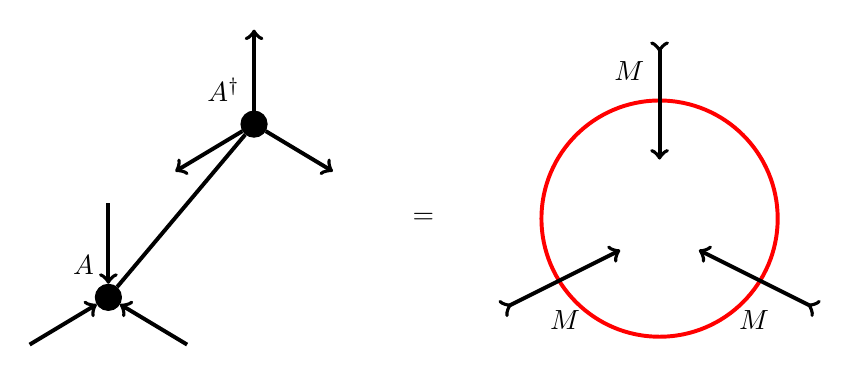
\begin{tikzpicture}
                \node[circle,draw=black,fill=black,minimum size=5pt,label={110:$A$}] (T) at (0,-1) {};
                \node[circle,draw=black,fill=black,minimum size=5pt,label={110:$A^\dag$}] (T2) at (1.85,1.2) {};
                \node (E) at (4,0) {$=$};
                \node[label={120:$M$}] (M1) at (7, 1.5) {};
                \node[label={-90:$M$}] (M2) at (8.2, -0.92) {};
                \node[label={-90:$M$}] (M3) at (5.8, -0.92) {};
                \draw[line width=0.5 mm] (T) -- (T2);
                \draw[<-, line width=0.5 mm] (T) -- +(0,1.2);
                \draw[<-, line width=0.5 mm] (T) -- (1, -1.6);
                \draw[<-, line width=0.5 mm] (T) -- (-1, -1.6);
                \draw[->, line width=0.5 mm] (T2) -- +(0,1.2);
                \draw[->, line width=0.5 mm] (T2) -- (2.85, 0.6);
                \draw[->, line width=0.5 mm] (T2) -- (0.85, 0.6);
                \draw[draw=red, line width=0.5 mm] (7, 0) circle (1.5);
                \draw[<-<, line width=0.5 mm] (7, 0.75) -- (7, 2.25);
                \draw[<-<, line width=0.5 mm] (7.5, -0.4) -- (9, -1.15);
                \draw[<-<, line width=0.5 mm] (6.5, -0.4) -- (5, -1.15);
            \end{tikzpicture}
            \caption{MPO-injective PEPS.}
            \label{tennet:fig:mpo_injectivity}
        \end{figure}
    }

    \begin{axiom}[Pulling-through]\index{pulling-through condition}
        One of the key features of topological order is that this cannot be detected locally, only a global measurement can show the existence of topologically ordered states. To this end we introduce an axiom such that one can pull an MPO through the lattice. Graphically this is shown in figure \ref{tennet:fig:pulling_through}.
        \begin{figure}[ht!]
            \centering
            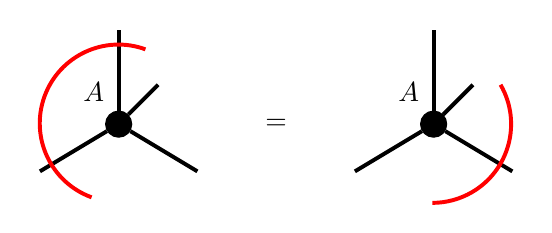
\begin{tikzpicture}
                \node[circle,draw=black,fill=black,minimum size=5pt,label={110:$A$}] (T) at (0,0) {};
                \node[circle,draw=black,fill=black,minimum size=5pt,label={110:$A$}] (T2) at (4,0) {};
                \node (E) at (2,0) {$=$};
                \draw[line width=0.5 mm] (T) -- +(0.5,0.5);
                \draw[line width=0.5 mm] (T) -- +(0,1.2);
                \draw[line width=0.5 mm] (T) -- (1, -0.6);
                \draw[line width=0.5 mm] (T) -- (-1, -0.6);
                \draw[line width=0.5 mm, draw=red] (0.34, 0.95) arc (70:250:1);
                \draw[line width=0.5 mm] (T2) -- +(0.5,0.5);
                \draw[line width=0.5 mm] (T2) -- +(0,1.2);
                \draw[line width=0.5 mm] (T2) -- (5, -0.6);
                \draw[line width=0.5 mm] (T2) -- (3, -0.6);
                \draw[line width=0.5 mm, draw=red] (4.85, 0.5) arc (30:-90:1);
            \end{tikzpicture}
            \caption{Pulling-through condition.}
            \label{tennet:fig:pulling_through}
        \end{figure}
    \end{axiom}

\subsection{MPO-symmetries for SPT phases}

    One can generalize the above framework to include not only pure topological order but also symmetry-protected topological order (see reference \cite{bultinck_mpo}). For this one has to slightly modify the axioms from the last section:
    \begin{axiom}[Pulling-through for SPT phases]\index{pulling-through condition}
        When pulling a symmetry-MPO through a tensor one has to act with a unitary on the physical level. Graphically this is shown in figure \ref{tennet:fig:pulling_through_spt}.
        \begin{figure}[ht!]
            \centering
            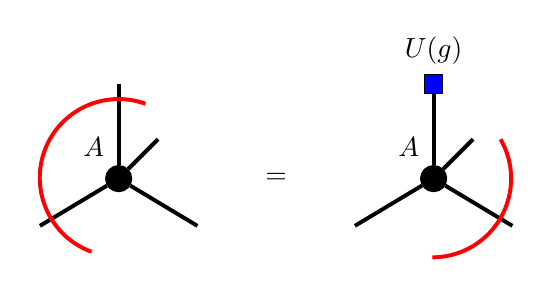
\begin{tikzpicture}
                \node[circle,draw=black,fill=black,minimum size=5pt,label={110:$A$}] (T) at (0,0) {};
                \node[circle,draw=black,fill=black,minimum size=5pt,label={110:$A$}] (T2) at (4,0) {};
                \node (E) at (2,0) {$=$};
                \draw[line width=0.5 mm] (T) -- +(0.5,0.5);
                \draw[line width=0.5 mm] (T) -- +(0,1.2);
                \draw[line width=0.5 mm] (T) -- (1, -0.6);
                \draw[line width=0.5 mm] (T) -- (-1, -0.6);
                \draw[line width=0.5 mm, draw=red] (0.34, 0.95) arc (70:250:1);
                \draw[line width=0.5 mm] (T2) -- +(0.5,0.5);
                \draw[line width=0.5 mm] (T2) -- +(0,1.2);
                \draw[line width=0.5 mm] (T2) -- (5, -0.6);
                \draw[line width=0.5 mm] (T2) -- (3, -0.6);
                \draw[line width=0.5 mm, draw=red] (4.85, 0.5) arc (30:-90:1);
                \node[rectangle, draw=black, fill=blue, minimum size=2pt, label={$U(g)$}] (U) at (4, 1.2) {};
            \end{tikzpicture}
            \caption{Pulling-through condition for SPT phases.}
            \label{tennet:fig:pulling_through_spt}
        \end{figure}
    \end{axiom}

%\chapter{Epilogue}
%
%    Since one of the main goals of this compendium was to keep me motivated to read papers and watch lectures about the various subjects under consideration, I should also add some of the seminal works that I hope to be able to understand  in the future, or at least be a able to skim through:
%
%    \begin{center}
%        \begin{tabular}{|c|l|}
%            \hline
%            Author&Title\\
%            \hline
%            Brown-Henneaux&Central charges in the canonical realization of \ldots\\
%			Bunke&Differential Cohomology\\
%			D'Auria-Fr\'e&Geometric supergravity in $D=11$ and its hidden supergroup\\
%			D'Auria-Fr\'e-Castellani&Supergravity and Superstrings: A Geometric Perspective\\
%            \textit{Friends}&Master's (and potentially PhD) theses\\
%            Fuchs-Runkel-Schweigert&TFT construction of RCFT correlators\\
%            Grothendieck&Pursuing Stacks\\
%            Lurie&Higher Topos Theory (\textit{book})\\
%            $\cdot$&On the Classification of Topological Field Theories\\
%            Schreiber&Differential cohomology in a cohesive $\infty$-topos\\
%            $\cdot$&Higher prequantum geometry\\
%            $\cdot$&Local prequantum field theory\\
%            \hline
%        \end{tabular}
%    \end{center}

\part{Appendices}
\begin{appendices}
\chapter{Derivations: Mathematics}

\section{Group theory}
\subsection{Explanation for property \ref{group:transitive_action_property}}\label{proof:stabilizer}

    Pick an element $x\in X$. The stabilizer of $x$ with respect to $G$ is the set \[S_x := \{g\in G:g\cdot x = x\}.\]
    Due to the transitivity of the group action we have that \[\forall x, y\in X: \exists h\in G: h\cdot x = y.\] So for every $z\in X$ we can choose a group element $g_z$ such that $g_z\cdot x = z$. For all elements in the coset $g_zS_x = \{g_zs\in G:s\in S_x\}$ the following equality is satisfied: \[(g_zs)\cdot x = g_z\cdot (s\cdot x) = g_z\cdot x = z.\] This implies that the map $\Phi:G/S_x \rightarrow X$ is surjective.

    Now we need to prove that $\Phi$ is also injective. We give a proof by contradiction. Choose two distinct cosets $gS_x$ and $hS_x$. Then there exist two elements $G, H\in X$ such that $g\cdot x = G$ and $h\cdot x = H$. Assume that $G = H$. This means that
    \begin{align*}
        &g\cdot x = h\cdot x\\
        \iff&(h^{-1}g)\cdot x = x\\
        \iff&h^{-1}g\in S_x\\
        \iff&hS_x\mathrel{\reflectbox{$\in$}}h(h^{-1}g) = g.
    \end{align*}
    This would imply that $gS_x = hS_x$ which is in contradiction with our assumptions. It follows that $G\neq H$ and hence that $\Phi$ is injective.\qed

\section{Calculus}
\subsection{Proof of method \ref{calculus:borel_transform}}

    The function $F(x)$ is defined as follows:
    \begin{gather}
        F(x) := \ds\sum_{n=0}^{+\infty}\stylefrac{a_n}{n!}x^n.
    \end{gather}
    We now perform a Borel transform:
    \begin{gather}
        \begin{array}{ccl}
            \ds\int_0^{+\infty}F(xt)e^{-t}dt&=&\ds\sum_{n=0}^N\int_0^{+\infty}\stylefrac{a_n}{n!}x^nt^ne^{-t}dt\\
            &=&\ds\sum_{n=0}^N\frac{a_n}{n!}x^n\int_0^{+\infty}t^ne^{-t}dt\\
            &=&\ds\sum_{n=0}^N\frac{a_n}{n!}x^n\Gamma(n+1)\\
            &=&\ds\sum_{n=0}^Na_nx^n
        \end{array}
   \end{gather}
   where we used the definition of the Gamma function \ref{calculus:gamma_function} on line 3 and the relation between the factorial function and the Gamma function \ref{calculus:gamma_factorial_relation} on line 4.\qed

\section{Linear algebra}
\subsection{Proof of equivalence of definitions \ref{tensor:exterior_algebra} and \ref{tensor:adef_exterior_algebra}}

    \begin{gather}
        (u+v)\otimes(u+v) - u\otimes u - v\otimes v = u\otimes v + v\otimes u
    \end{gather}
    The LHS is an element of the ideal $I$ generated by $\{v\otimes v;v\in V\}$. Using the ideal generated by elements such as in the RHS gives the usual definition of the exterior algebra based on the wedge product as defined in \ref{tensor:wedge_product} because it imposes the relation $u\wedge v = -v\wedge u$.

    We do however have to pay attention to one little detail. As mentioned in \ref{tensor:adef_exterior_algebra} the general definition uses the ideal $I$ to construct the quotient space. The other construction is only equivalent when are working over a field with characteristic different from 2. This follows from the fact that we have to divide by 2 when trying to obtain the ideal $I$ from the RHS when setting $u=v$.

\section{Manifolds and bundles}
\subsection{Proof of equivalence of definitions \ref{diff:tangent_vector_partial} and \ref{diff:alternative_definition}}

    Let $(U, \varphi)$ be a chart around the point $p\in M$. Using the first definition of a tangent vector (\ref{diff:tangent_vector_partial}), i.e. \[\left.\ds\pderiv{}{q^i}\right|_{p}:\mathcal{F}_p(M, \mathbb{R})\rightarrow\mathbb{R}:f\mapsto \pderiv{}{q^i}\left(f\circ\varphi^{-1}\right)(\varphi(p))\] we can rewrite equation \ref{diff:tangent_vector_chain_rule} \[v_p(f) = \pderiv{(f\circ\varphi^{-1})}{q^i}(\varphi(p))\deriv{q^i}{t}(0)\] as follows: \[v_p(f) = \left.\pderiv{f}{q^i}\right|_p\deriv{q^i}{t}(0).\] Because the partial derivatives as defined in \ref{diff:tangent_vector_partial} form a basis for the tangent space (by construction), we see that this equation is in fact an expansion of the tangent vector $v_p$ in terms of that basis. It follows that vectors tangent to curves\footnote{More precisely: representatives of equivalence classes of vectors tangent to curves.} are also tangent vectors according to the first definition.

    To prove the other direction we have to show that the partial derivative operators can be constructed as vectors tangent to curves.

    A tangent vector can be expressed, according to the first construction, in the following way:
    \[
        v_p = v^i\left.\pderiv{}{q^i}\right|_p
    \]
    where we also define $v = (v^1, ..., v^n)$. We can then construct the curve $\gamma: t\mapsto \varphi^{-1}(q_0+vt)$. It is obvious that the tangent vector $v_p$ is tangent to the curve $\gamma$. From this it follows that we have an isomorphism between the tangent vectors from to the first definition and the equivalence classes of vectors tangent to curves from the second definition. These definitions are thus equivalent.\qed

    Although the previous equivalence implies that the tangent space construction using germs of curves gives us a vector space we could also check the vector space axioms directly. First we prove that the sum of vectors tangent to the curves $\gamma$ and $\delta$ is again a vector tangent to some curve $\chi:\mathbb{R}\rightarrow M$. For this let us define the curve \[\chi(t) \equiv \varphi^{-1}\circ\Big(\varphi\circ\gamma(t) + \varphi\circ\delta(t) - \varphi(p)\Big)\] where $\varphi$ is again the coordinate map in some chart $(U, \varphi)$ around $p\in M$. Using equation \ref{diff:tangent_vector_chain_rule} we find
    \begin{align*}
        v_{p, \chi}(f) &= \pderiv{(f\circ\varphi^{-1})}{q^i}(\varphi(p))\deriv{(\varphi^i\circ\chi)}{t}(0)\\
        &=\pderiv{(f\circ\varphi^{-1})}{q^i}(\varphi(p))\deriv{}{t}\left(\varphi^i\circ\gamma + \varphi^i\circ\delta - \varphi^i(p)\right)\\
        &=\pderiv{(f\circ\varphi^{-1})}{q^i}(\varphi(p))\left(\deriv{(\varphi^i\circ\gamma)}{t} + \deriv{(\varphi^i\circ\delta)}{t}\right)\\
        &=v_{p, \gamma}(f) + v_{p, \delta}(f).
    \end{align*}
    The constant term $-\varphi(p)$ in the definition of $\chi(t)$ is necessary to make sure that $\chi(0) = \gamma(0) = \delta(0) = p$. The scalar multiplication by a number $\lambda\in K$ can be proven by defining the curve $\chi(t) = \varphi^{-1}\circ\left[\lambda\Big(\varphi\circ\gamma(t)\Big)\right]$.

\subsection{Explanation for example \ref{diff:lie_derivative_function}}\index{Landau!little-o notation}

    In this derivation we use the Landau little-o notation $o(t)$, i.e.:
    \begin{gather}
        \lim_{t\rightarrow0}\frac{o(t)}{t} = 0
    \end{gather}
    Now assume that $X$  is a smooth vector field and $f$ is a smooth function. Because the Lie derivative is a local operation we can work in a local chart such that $\gamma$ is (again locally) equivalent to a curve\footnote{The vector field $X(p) = (p, Y(p))$ where $Y$ is a smooth vector field on $\mathbb{R}^n$ can also be identified with $Y$ itself. This is implicitly done in the derivation by using the notation $X$ for both vector fields.} $\beta_p:U\rightarrow\mathbb{R}^n$ and such that we can expand $\beta_p(t)$ around $p\in U$:
    \begin{align}
        \mathcal{L}_Xf(p) &= \lim_{t\rightarrow0}\left[\stylefrac{f(\beta_p(0) + t\beta_p'(0) + o(t)) - f(p)}{t}\right]\nonumber\\
        &= \lim_{t\rightarrow0}\left[\stylefrac{f(p + tX(p) + o(t)) - f(p)}{t}\right]\nonumber\\
        &= \lim_{t\rightarrow0}\left[\stylefrac{f(p) + tDf(p)\cdot X(p) + o(t) - f(p)}{t}\right]\nonumber\\
        &= \sum_k\pderiv{f}{x^k}(p)X_k(p) + \lim_{t\rightarrow0}\stylefrac{o(t)}{t}\nonumber\\
        &= \sum_k\pderiv{f}{x^k}(p)X_k(p)\label{manifolds:lie_derivative_calc}
    \end{align}
    where we used the defining condition \ref{diff:integral_curve} for integral curves on the second line. If we now rewrite this equation as an operator equality, we obtain
    \begin{gather}
        \mathcal{L}_X = \sum_kX_k\pderiv{}{x^k}.
    \end{gather}

\subsection{Explanation for formula \ref{diff:lie_derivative_vector_field}}

    For vector fields we cannot just take the difference at two different points because the tangent spaces generally do not coincide. We can solve this by using the flow \ref{diff:flow}:
    \begin{gather}
        \label{derivmath:lie_derivative_vector_fields}
        \mathcal{L}_XY = \lim_{t\rightarrow0}\stylefrac{(T\sigma_t)^{-1}[X(\gamma_p(t))] - X(p)}{t}
    \end{gather}
    where the $T\sigma_t$ is the differential \ref{diff:differential} of the flow which satisfies $(T\sigma)^{-1} = T\sigma_{-t}$. To see that this definition makes sense we have to show that $(T\sigma_t)^{-1}[X(\gamma_p(t))]\in T_pM$. This goes as follows:
    \begin{align*}
        (T\sigma_t)^{-1}[X(\gamma_p(t))](f) &= T\sigma_{-t}[X(\gamma_p(t))](f)\\
        &= X(\sigma_{-t}\circ\gamma_p(t))(f\circ\sigma_{-t})\\
        &= X(\sigma_{-t}\circ\sigma_t(p))(f\circ\sigma_{-t})\\
        &= X(p)(f\circ\sigma_{-t})\\
        &\in T_pM
    \end{align*}
    for all $f\in C^k(M, \mathbb{R})$. On the third line we used the definition of the flow \ref{diff:flow}.

    We can also rewrite the second term in the numerator of \ref{derivmath:lie_derivative_vector_fields} using the flow: \[X(p) = X(\sigma_0(p)) = T\sigma_0(X)\] Using the definition of the pushforward of vector fields \ref{diff:pushforward} the Lie derivative can be rewritten as follows:
    \begin{align*}
        \mathcal{L}_XY &= \lim_{t\rightarrow0}\stylefrac{\sigma_{-t*}X(\gamma_p(t)) - \sigma_{0*}X(\gamma_p(0))}{t}\\
        &= \left.\deriv{}{t}(\sigma_{-t*}X)(\gamma_p(t))\right|_{t=0}.
    \end{align*}
    Or finally by using the relation between pushforward and pullback \ref{diff:pullback_pushforward} this becomes
    \begin{gather}
        \mathcal{L}_XY = \left.\deriv{}{t}(\sigma_t^*X)(\gamma_p(t))\right|_{t=0}.
    \end{gather}

\subsection{Explanation of remark \ref{diff:vector_calculus}}

    Looking at formula \ref{diff:function_derivative} for the exterior derivative of a smooth function and remembering the definition of the gradient \ref{vectorcalculus:gradient} we see that these two definitions appear very similar. The major difference lies in the fact that $\nabla f$ is a vector in $\mathbb{R}^3$ and $df$ is a covector in $\mathbb{R}^{*3}$. However there exists an isomorphism between these spaces and so we can identify $\nabla f$ and $df$.

    Similar relations hold for the rotor \ref{vectorcalculus:rotor} and divergence \ref{vectorcalculus:divergence}, however here we have to use a different construction as we will be working with the spaces $\Lambda^1$ and $\Lambda^2$. However we can use the Hodge star \ref{tensor:hodge_star} to obtain the correct dimensions.

    Consider a vector $\vector{f} = (f_1, f_2, f_3)$ where $f_i$ is smooth. Using these functions $f_i$ we can construct a 1-form $\alpha = f_1dx_1 + f_2dx_2 + f_3dx_3$ and a 2-form $\omega = f_1dx_2\wedge dx_3 + f_2dx_3\wedge dx_1 + f_3 dx_1\wedge dx_2$. After applying the exterior derivative (in the corresponding spaces) we obtain
    \begin{align}
        d\alpha &= \left(\pderiv{f_3}{x_2} - \pderiv{f_2}{x_3}\right)dx_2\wedge dx_3 + \left(\pderiv{f_1}{x_3} - \pderiv{f_3}{x_1}\right)dx_3\wedge dx_1 + \left(\pderiv{f_2}{x_1} - \pderiv{f_1}{x_2}\right)dx_1\wedge dx_2 \nonumber\\
        d\omega &= \left(\pderiv{f_1}{x_1} + \pderiv{f_2}{x_2} + \pderiv{f_3}{x_3}\right)dx_1\wedge dx_2\wedge dx_3. \nonumber
    \end{align}
    Using result \ref{tensor:hodge_star_vectorcalculus} and the canonical isomorphism $\sim\ :\mathbb{R}^{3*}\rightarrow\mathbb{R}^3$ we can rewrite this as
    \begin{align}
        \sim df &= \nabla f \\
        \sim (\ast d\alpha) &= \nabla\times\vector{f} \\
        \ast d\omega &= \nabla\cdot\vector{f}.
    \end{align}
\chapter{\texorpdfstring{$G$-Structures}{G-Structures}}
    In the following table we give an overview of the more common $G$-structures one can define on a smooth (simply-connected) manifolds $M^n$.
    \begin{center}
        \begin{tabularx}{\textwidth}{|l|c|X|}
             \hline
                 Geometric structure&Structure group&Remarks\\
             \hline
                 Orientation&$\text{SL}(n,\mathbb{R})$&$\text{GL}^+(n, \mathbb{R})$ is sufficient for orientability. The special linear group gives rise to a volume form.\\
                 Riemannian metric&$O(n)$&\\&&\\
                 Almost-symplectic structure*&$\text{Sp}(n,\mathbb{R})$&Integrability (in the form of a closed form) gives a symplectic manifold.\\&&\\
                 Almost-complex structure*&$\text{GL}(k, \mathbb{C})$&Integrability (in the form of Newlander-Nirenberg) gives a complex manifold.\\&&\\
                 Almost-Hermitian structure*&$\text{U}(k)$&Integrability gives a K\"ahler manifold.\\&&\\
                 Calabi-Yau*&$\text{SU}(k)$&\\&&\\
                 Hyperk\"ahler**&$\text{Sp}(k)$&Hyperk\"ahler implies Calabi-Yau.\\&&\\
                 Almost quaternionic**&$(\text{GL}(k,\mathbb{H})\times\mathbb{H}^\times)/\mathbb{R}^\times$&Integrability gives a quaternionic manifold. We also require $k\geq2$ because for $k=1$ we would otherwise obtain that every orientable 4-manifold is quaternionic (amongst other things).\\&&\\
                 Quaternionic-K\"ahler**&$(\text{Sp}(k)\times\text{Sp}(1))/\mathbb{Z}_2$&These manifolds are not strictly K\"ahler since the structure group is not a subgroup of $\text{U}(2k)$.\\
             \hline
        \end{tabularx}
    \end{center}
    Structures marked with $\ast$ require the real dimension $n=2k$ to be even. Structures marked with $\ast\ast$ require the real dimension $n=4k$ to be a multiple of 4.

    \begin{remark*}
        This table is strongly related\footnote{The SL$(n, \mathbb{R})$-structure is technically not part of the original classification since it is not a subgroup of O$(n)$ and hence the manifold is not necessarily Riemannian.} to the classification of (\textit{irreducible} simply-connected \textit{nonsymmetric}) Riemannian manifolds by \textit{Berger}. A more general classification for manifolds which are not necessarily Riemannian was initiated by Berger and finished by others. However we will only mention this extension here, for references see \cite{diffgeom_physics}.

        Since not all concepts from this classification were defined throughout the compendium we will explain them here:
        \begin{itemize}
            \item \textbf{Irreducible}: A Riemannian manifold is said to be irreducible if it is not locally isomorphic to a product of Riemannian manifolds.
            \item \textbf{Symmetric}\footnote{or \textbf{locally symmetric}}: A smooth manifold, locally modelled on $V\cong\mathbb{R}^n$, is said to be symmetric if the curvature mapping $F(M)\rightarrow\Lambda^2V^*\otimes\mathfrak{g}$ is covariantly constant.
        \end{itemize}
    \end{remark*}

    \begin{remark}
        Although most manifolds from the above list admit an explicit definition, the quaternionic K\"ahler manifolds are exactly defined by their structure group/holonomy group.

        It is also clear that hyperk\"ahler manifolds are a specific class of quaternionic K\"ahler manifolds since Sp$(k)$ can be embedded in Sp$(k)\cdot\text{Sp}(1)$. To exclude this class we can just require the holonomy group to be all of Sp$(k)\cdot\text{Sp}(1)$. This is equivalent to requiring that quaternionic K\"ahler manifolds have a nonvanishing scalar curvature. This is related to the following property:
    \end{remark}
    \begin{property}
        Every quaternionic K\"ahler manifold is Einstein \ref{diff:einstein_manifold}. The hyperk\"ahler manifolds are then exactly the quaternionic K\"ahler manifolds with vanishing scalar curvature (which is constant by the manifold being Einstein).
    \end{property}
\chapter{Derivations: Mathematical Physics}
\section{d'Alembert's principle}\label{deriv:lagrange}\index{Lagrangian}

    In the following derivation we assume the mass to be constant.
    \begin{align}
        &\sum_k \left(\vector{F}_k - \dot{\vector{p}}_k\right)\dot{\vector{r}}_k = 0\nonumber\\
        \iff&\sum_k \left(\vector{F}_k - \dot{\vector{p}}_k\right)\cdot\left(\sum_l\pderiv{\vector{r}}{q_l}\dot{q_l}\right) = 0\nonumber\\
        \iff&\sum_l\left(\sum_k\vector{F}_k\cdot\pderiv{\vector{r}}{q_l} - \sum_km\ddot{\vector{r}}\cdot\pderiv{\vector{r}}{q_l}\right)\dot{q_l} = 0\nonumber\\
        \iff&\sum_l\left(Q_l - \sum_km\ddot{\vector{r}}\cdot\pderiv{\vector{r}}{q_l}\right)\dot{q_l} = 0\label{lagrange_deriv:deriv1}
    \end{align}
    \noindent Now we look at the following derivative:
    \begin{align}
        &\deriv{}{t}\left(\dot{\vector{r}}\cdot\pderiv{\vector{r}}{q_l}\right) = \ddot{\vector{r}}\cdot\pderiv{\vector{r}}{q_l} + \dot{\vector{r}}\cdot\deriv{}{t}\left(\pderiv{\vector{r}}{q_l}\right)\nonumber\\
        \iff&\ddot{\vector{r}}\cdot\pderiv{\vector{r}}{q_l} = \deriv{}{t}\left(\dot{\vector{r}}\cdot\pderiv{\vector{r}}{q_l}\right) - \dot{\vector{r}}\cdot\deriv{}{t}\left(\pderiv{\vector{r}}{q_l}\right)\nonumber\\
        \iff&\ddot{\vector{r}}\cdot\pderiv{\vector{r}}{q_l} = \deriv{}{t}\left(\dot{\vector{r}}\cdot{\color{red}\underbrace{\textcolor{black}{\pderiv{\vector{r}}{q_l}}}_A}\right) - \dot{\vector{r}}\cdot\left(\pderiv{\dot{\vector{r}}}{q_l}\right).\label{lagrange_deriv:deriv2}
    \end{align}
    To evaluate A we can take a look at another derivative:
    \begin{align}
        \pderiv{\dot{\vector{r}}}{\dot{q}_l} &= \pderiv{}{\dot{q}_l}\left(\sum_k\pderiv{r}{q_k}\dot{q}_k\right)\nonumber\\
        &=\sum_k\pderiv{r}{q_k}\delta_{kl}\nonumber\\
        &=\pderiv{\vector{r}}{q_l}\nonumber\\
        &=\textcolor{red}{A}.\nonumber
    \end{align}
    Substituting this in formula \ref{lagrange_deriv:deriv2} gives
    \begin{align}
        \ddot{\vector{r}}\cdot\pderiv{\vector{r}}{q_l} &= \deriv{}{t}\left(\dot{\vector{r}}\cdot\pderiv{\dot{\vector{r}}}{\dot{q}_l}\right) - \dot{\vector{r}}\cdot\left(\pderiv{\dot{\vector{r}}}{q_l}\right)\nonumber\\
        &=\deriv{}{t}\left(\stylefrac{1}{2}\pderiv{\dot{\vector{r}}^2}{\dot{q}_l}\right) - \stylefrac{1}{2}\pderiv{\dot{\vector{r}}^2}{q_l}.\label{lagrange_deriv:deriv3}
    \end{align}
    If we multiply this by the mass $m$ and sum over all particles we get
    \begin{align}
        \sum_km_k\ddot{\vector{r}}_k\cdot\pderiv{\vector{r}_k}{q_l}=\ &\deriv{}{t}\pderiv{}{\dot{q}_l}\left(\sum_k\stylefrac{1}{2}m\dot{\vector{r}}_k^2\right) - \pderiv{}{q_l}\left(\sum_k\stylefrac{1}{2}m\dot{\vector{r}}_k^2\right)\nonumber\\
        =\ &\deriv{}{t}\pderiv{T}{\dot{q}_l} - \pderiv{T}{q_l}\label{lagrange_deriv:deriv4}
    \end{align}
    where we have denoted the total kinetic energy in the last line by $T$. Plugging this result into formula \ref{lagrange_deriv:deriv1} gives us
    \begin{gather}
        \label{lagrange_deriv:deriv5}
        \sum_l\left(Q_l - \deriv{}{t}\pderiv{T}{\dot{q}_l} - \pderiv{T}{q_l}\right)\dot{q_l} = 0.
    \end{gather}
    As all the $q_l$ are independent the following relation should hold for all $l$:
    \begin{align}
        &Q_l - \deriv{}{t}\left(\pderiv{T}{\dot{q}_l}\right) - \pderiv{T}{q_l} = 0\nonumber\\
        \iff&\deriv{}{t}\left(\pderiv{T}{\dot{q}_l}\right) - \pderiv{T}{q_l} = Q_l.\label{lagrange_deriv:first_kind}
    \end{align}
    This last equation is known as a \textbf{Lagrange equation of the first kind}.

    If we have a system with only conservative forces acting on it, we can write the force on the $i^{th}$ particle as
    \begin{gather}
        \label{lagrange_deriv:deriv7}
        F_i = -\nabla_iV.
    \end{gather}
    With this in mind, let's take a look at the derivative of the potential $V$ with respect to the $l^{th}$ generalized coordinate:
    \begin{gather}
        \label{lagrange_deriv:deriv8}
        \begin{aligned}
            \pderiv{V}{q_l} &= \sum_i\left(\nabla_iV\right)\cdot\pderiv{\vector{r}_i}{q_l}\\
            &=-Q_l.
        \end{aligned}
    \end{gather}
    The derivative of $V$ with respect to any generalized velocity $\dot{q}_l$ is trivially zero. This combined with the previous formula and with formula \ref{lagrange_deriv:first_kind} gives
    \begin{align}
        &\deriv{}{t}\left(\pderiv{T}{\dot{q}_l}\right) - \pderiv{T}{q_l} = Q_l\nonumber\\
        \iff&\deriv{}{t}\left(\pderiv{T}{\dot{q}_l}\right) - \pderiv{T}{q_l} = -\pderiv{V}{q_l} + \pderiv{V}{\dot{q}_l}\nonumber\\
        \iff&\deriv{}{t}\left(\pderiv{T}{\dot{q}_l} - \pderiv{V}{\dot{q}_l}\right) - \pderiv{}{q_l}\left(T - V\right) = 0.\label{lagrange:deriv9}
    \end{align}
    If we introduce a new variable $L:=T-V$, called the \textbf{Lagrangian}, we get the \textbf{Lagrangian equation of the second kind}:
    \begin{gather}
        \label{lagrange_deriv:second_kind}
        \deriv{}{t}\left(\pderiv{L}{\dot{q}_l}\right) - \pderiv{L}{q_l} = 0.
    \end{gather}

\section{Hamilton's principle}

    In this part we start from the principle of least action. First we recall the definition of the \textbf{action}:
    \begin{gather}
        \label{lagrange_deriv:action_integral}
        I[y] := \int_{t_1}^{t_2}L\left(y(t), \dot{y}(t), t\right)dt
    \end{gather}
    Now we want to require that this action is minimal for the physically relevant path (Hamilton's principle). To do this we define a family of paths:
    \begin{gather}
        \label{lagrange_deriv:family_of_paths}
        y(t, \alpha) = y(t) + \alpha\eta(t)
    \end{gather}
    where $\eta(t)$ is an arbitrary function with the following boundary conditions:
    \begin{gather}
        \begin{cases}
        \eta(t_1) = 0&\\
        \eta(t_2) = 0.&
        \end{cases}
    \end{gather}
    If we define the action integral over this family of paths, the integral \ref{lagrange_deriv:action_integral} becomes a function of $\alpha$:
    \begin{gather}
        \label{lagrange_deriv:action_integral_over_family}
        I(\alpha) = \int_{t_1}^{t_2}L\left(y(t,\alpha), \dot{y}(t, \alpha), t\right)dt.
    \end{gather}
    Requiring that the action integral is stationary for $y(t)$ (and thus $\alpha = 0$) is equivalent to
    \begin{gather}
        \label{lagrange_deriv:stationary_condition}
        \left(\deriv{I}{\alpha}\right)_{\alpha=0} = 0.
    \end{gather}
    This condition combined with formula \ref{lagrange_deriv:action_integral_over_family} gives us
    \begin{gather}
        \label{lagrange_deriv:derivative_of_integral}
        \deriv{I}{\alpha} = \int_{t_1}^{t_2}\deriv{}{\alpha}L\left(y(t,\alpha), \dot{y}(t, \alpha), t\right)dt.
    \end{gather}
    As we evaluate this derivative at $\alpha = 0$ we can replace $y(t, \alpha)$ by $y(t)$ due to definition \ref{lagrange_deriv:family_of_paths}.
    \begin{align}
        \deriv{I}{\alpha}&=\int_{t_1}^{t_2}\left[\pderiv{L}{y}\pderiv{y}{\alpha} + \pderiv{L}{\dot{y}}\pderiv{\dot{y}}{\alpha}\right]dt\nonumber\\
        &=\int_{t_1}^{t_2}\left[\pderiv{L}{y}\eta(t) + \pderiv{L}{\dot{y}}\dot{\eta}(t)\right]dt.
    \end{align}
    If we substitute $\pderiv{L}{\dot{y}} := h(t)$ and apply integration by parts to the second term in this integral, we get
    \begin{align}
        \deriv{I}{\alpha}&=\int_{t_1}^{t_2}\left[\pderiv{L}{y}\eta(x) + h(t)\dot{\eta}(t)\right]dt\nonumber\\
        &=\int_{t_1}^{t_2}\left[\pderiv{L}{y}\eta(t) + h(t)\deriv{\eta}{t}\right]dt\nonumber\\
        &=\int_{t_1}^{t_2}\pderiv{L}{y}\eta(t)dt + \eta(t_2)h(t_2) - \eta(t_1)h(t_1) - \int_{t_1}^{t_2}\deriv{}{t}\left(\pderiv{L}{\dot{y}}\right)\eta(t)dt.
    \end{align}
    Due to the initial conditions \ref{lagrange_deriv:stationary_condition} for the function $\eta(t)$, the two terms in the middle vanish and we obtain
    \begin{gather}
        \label{lagrange_deriv:final_integral}
        \deriv{I}{\alpha}=\int_{t_1}^{t_2}\left[\pderiv{L}{y} - \deriv{}{t}\left(\pderiv{L}{\dot{y}}\right)\right]\eta(t)dt.
    \end{gather}
    Furthermore, since the function $\eta(t)$ was arbitrary, the only possible way that this derivative can become zero is when the integrand is identically zero:
    \begin{gather}
        \label{lagrange_deriv:second_kind_with_hamilton}
        \pderiv{L}{y} - \deriv{}{t}\left(\pderiv{L}{\dot{y}}\right) = 0.
    \end{gather}
    If we compare this result with formula \ref{lagrange_deriv:second_kind} we see that we can also obtain the \textbf{Lagrangian equations of the second kind} by starting from the principle of least action. (Where the variable $y$ represents the generalized coordinates $q_l$ and the variable $\dot{y}$ represents the generalized velocities $\dot{q}_l$)

    \begin{remark}
        Differential equations of the form
        \begin{gather}
            \label{lagrange_deriv:euler_lagrange_equation}
            \pderiv{f}{y}(y, \dot{y}, x) = \deriv{}{x}\left(\pderiv{f}{\dot{y}}(y, \dot{y}, x)\right)
        \end{gather}
        are known as \textbf{Euler-Lagrange equations}.
    \end{remark}

\section{Noether's theorem \ref{qft:noethers_theorem}}\label{proof:noether}

    The general transformation rule for the Lagrangian is
    \begin{gather}
        \label{noether_deriv:1}
        \mathcal{L}(x)\rightarrow\mathcal{L}(x) + \alpha\ \delta\mathcal{L}(x).
    \end{gather}
    To have a symmetry, i.e. to keep the action invariant, the deformation factor has to be a 4-divergence:
    \begin{gather}
        \label{noether_deriv:2}
        \mathcal{L}(x)\rightarrow\mathcal{L}(x) + \alpha\partial_\mu\mathcal{J}^\mu(x).
    \end{gather}

    To obtain formula \ref{qft:conserved_current} we vary the Lagrangian explicitly:
    \begin{align*}
        \delta\mathcal{L} &= \pderiv{\mathcal{L}}{\phi}\delta\phi + \pderiv{\mathcal{L}}{(\partial_\mu\phi)}\delta(\partial_\mu\phi)\\
        &= \pderiv{\mathcal{L}}{\phi}\delta\phi + \partial_\mu\left(\pderiv{\mathcal{L}}{(\partial_\mu\phi)}\delta\phi\right) - \partial_\mu\left(\pderiv{\mathcal{L}}{(\partial_\mu\phi)}\right)\delta\phi\\
        &= \partial_\mu\left(\pderiv{\mathcal{L}}{(\partial_\mu\phi)}\delta\phi\right) + \left[\pderiv{\mathcal{L}}{\phi} - \pderiv{\mathcal{L}}{(\partial_\mu\phi)}\right]\delta\phi.
    \end{align*}
    The second term vanishes due to the Euler-Lagrange equation \ref{lagrange_deriv:second_kind_with_hamilton}. Combining these formulas gives us
    \begin{gather}
        \partial_\mu\left(\pderiv{\mathcal{L}}{(\partial_\mu\phi)}\delta\phi\right) - \partial_\mu\mathcal{J}^\mu(x) = 0.
    \end{gather}
    From this equation we can conclude that the current
    \begin{gather}
        j^\mu(x) = \pderiv{\mathcal{L}}{(\partial_\mu\phi)}\delta\phi - \mathcal{J}^\mu(x)
    \end{gather}
    is conserved.


\chapter{Derivations: Optics and Material Physics}

\section{Law of Lambert-Beer \ref{optics:lambert_beer}}

    From formula \ref{optics:dielectric_function_non_magnetic} we now that the complex refractive index can be written as \[\widetilde{n} = n+ik\] where $k$ is called the \textbf{extinction coefficient}. From classic optics we also know that in a material the speed of light obeys the following relation: \[c = \widetilde{n}v.\] It readily follows that the wave number (sadly also denoted by the letter $k$) can be written as \[k = \stylefrac{\omega}{v} = \widetilde{n}\stylefrac{\omega}{c}.\] From classic electromagnetism we know that a plane wave can be written as \[E(x, t) = \text{Re}\big\{A\ \text{exp}\left[i(kx - \omega t + \phi)\right]\big\}.\] So after putting everything together we obtain \[E(x, t) = \text{Re}\left\{A\ \text{exp}\left[i\left((n+ik)\stylefrac{\omega}{c}x - \omega t + \phi\right)\right]\right\}.\] or also:\[E(x, t) = \text{Re}\left\{A\ \text{exp}\left(in\stylefrac{\omega}{c}x\right)\cdot\text{exp}\left(-k\stylefrac{\omega}{c}x\right)\cdot\text{exp}\left(-i\omega t\right)\cdot\text{exp}\left(i\phi\right)\right\}\] We also know that the intensity is given by the following relation:\[I(x) = |E(x)|^2 = E^*(x)\cdot E(x).\]
    This implies that only the second exponential factor will remain. Dividing the result by its value at $x=0$ gives \[\stylefrac{I(x)}{I(0)} = \stylefrac{E(x)\cdot E^*(x)}{E(0)\cdot E^*(0)} = \text{exp}\left(-\stylefrac{2k\omega}{c}x\right) = \text{exp}(-\alpha x)\]
    where $\alpha$ is the absorption coefficient as defined in formula \ref{optics:absorption_coefficient}.\qed

\section{Schottky defects \ref{maphy:schottky_defects}}\label{deriv:schottky_defects}\index{Schottky!defect}\index{Frenkel pair}

    Let $E_v$ be the energy needed to remove a particle from its lattice point and move it to the surface. We will neglect any surface effects and assume that the the energy $E_v$ is independent of the distance to the surface.

    The total energy of all vacancies is then given by $E = nE_v$. The number of possible microstates is
    \begin{gather}
        \Omega = \stylefrac{(N+n)!}{N!n!}
    \end{gather}
    where we used the fact that the removal of $n$ particles creates $n$ more lattice points at the surface. Using Boltzmann's entropy formula \ref{statmech:boltzmann_formula} and Stirling's formula we obtain
    \begin{gather}
        S(N, n) = k\ln\Omega = k\big[(N+n)\ln(N+n) -n\ln n - N\ln N \big].
    \end{gather}
    Using \ref{statmech:temperature} we can find the temperature
    \begin{gather}
        \stylefrac{1}{T} = \left(\pderiv{S}{E}\right)_{N, V} = \deriv{S}{n}\deriv{n}{E} = \frac{k}{E_v}\ln\frac{N+n}{n}
    \end{gather}
    which can be rewritten as
    \begin{gather}
        \stylefrac{n}{N + n} = \exp\left(-\frac{E_v}{kT}\right).
    \end{gather}
    The density of Frenkel pairs can be derived analogously.

\chapter{Derivations: Classical Mechanics}

\section{Moments of inertia}\label{deriv:inertia}\index{inertia}

    In this section we will use formula \ref{forces:moment_of_inertia} to calculate the moment of inertia.

\subsection{Disk}

    The volume of a (solid) disk is given by
    \begin{gather}
        V_{disk} = \pi R^2d
    \end{gather}
    where $R$ is the radius and $d$ is the thickness. The mass density is then given by
    \begin{gather}
        \rho = \frac{M}{\pi R^2d}.
    \end{gather}
    Using cylindrical coordinates the moment of inertia becomes
    \begin{align}
        I &= \frac{M}{\pi R^2d}\int_0^{2\pi}d\varphi\int_0^ddz\int_0^Rr^3dr\\
        &= \frac{M}{\pi R^2d}2\pi d\frac{R^4}{4}\\
        &= \frac{1}{2}MR^2.
    \end{align}

\subsection{Solid sphere}

    The volume of a solid sphere is given by
    \begin{gather}
        V_{sphere} = \frac{4}{3}\pi R^3
    \end{gather}
    where $R$ is the radius. The mass density is then given by
    \begin{gather}
        \rho = \frac{M}{\frac{4}{3}\pi R^3}.
    \end{gather}
    We will use spherical coordinates to derive the moment of inertia, but we have to be careful. The $r$ in formula \ref{forces:moment_of_inertia} is the distance between a point in the body and the axis of rotation. So it is not the same as the $r$ in spherical coordinates which is the distance between a point and the origin. However, the relation between these two quantities is easily found using basic geometry to be:
    \begin{gather}
        r = r'\sin\theta
    \end{gather}
    where $r'$ is the spherical coordinate. Now we can calculate the moment of inertia as follows:
    \begin{align}
        I &= \frac{M}{\frac{4}{3}\pi R^3} \int_0^{2\pi}d\varphi\int_0^Rr'^{^4}dr'\int_0^\pi\sin^3\theta d\theta\\
        &= \frac{M}{\frac{4}{3}\pi R^3} 2\pi \frac{R^5}{5} \frac{4}{3}\\
        &= \frac{2}{5}MR^2.
    \end{align}
\chapter{Scribblings}
\section{Functorial uncertainty measures}
\subsection{Uncertainty}

    Let us for now assume that we work on finite spaces $\Omega$, i.e. $|\Omega|<\infty$. In this case one can characterize a probability measure as a set-theoretic function $P:2^\Omega\rightarrow[0, 1]$ with the following properties:
    \begin{enumerate}
        \item $P(\emptyset) = 0$ and $P(\Omega) = 1$;
        \item Additivity: If $A,B\subset\Omega$ are disjoint, then
            \begin{gather}
                \label{scrib:additive}
                P(A\cup B) = P(A) + P(B).
            \end{gather}
    \end{enumerate}
    When we want to quantify the uncertainty in the prediction of a random variable $X$ we can also take the cardinality of all possible values of $X$ as an indicator, i.e. a situation where we predict that $X$ can take on a value in $\{1, 2, 3, 4, 5\}$ has more uncertainty than a prediction where $X\in\{1, 2\}$. From the logical side we can characterize this through an indicator function $\Pi:2^\Omega\times2^\Omega\rightarrow\{0, 1\}$ where given a subset $Z$ the function $\Pi_Z$ tells us if a prediction $W\in2^\Omega$ has any overlap with $Z$. (Here the cardinality of the set $Z$ quantifies the degree of uncertainty, the larger $Z$ the less certain we are.) This function should satisfy the following conditions:
    \begin{enumerate}
        \item $\Pi_Z(\emptyset) = 0$;
        \item $\Pi_Z(\Omega) = 1$;
        \item Maxitivity\footnote{I didn't invent this name.}: If $A,B\subset\Omega$ are disjoint, then
            \begin{gather}
                \label{scrib:maxitive}
                P_Z(A\cup B) = \max(P_Z(A), P_Z(B)).
            \end{gather}
    \end{enumerate}

\subsection{Posets and categories}

    We know want to unify these notions and for this we need to find the common structure behind addition and taking maxima. For this it is better if we consider the (co)domains of our operations as posets (partially ordered sets) and their associated categorical structure:
    \newdef{Poset}{
        A set $X$ wih a binary operation $\leq$ that satisfies the following conditions:
        \begin{enumerate}
            \item Reflexivity: $x\leq x$;
            \item Antisymmetry: $x\leq y\land y\leq x\implies x=y$;
            \item Transitivity: $x\leq y\land y\leq z\implies x\leq z$.
        \end{enumerate}
    }
    \newprop{Posets are categories}{
        Let $(X, \leq)$ be a poset. This set admits the structure of a category $\mathbf{X}$ by taking $\ob{X}:=X$ and \[\hom_{\mathbf{X}}(a, b)=\begin{cases}
            \{\ast\}&a\leq b\\
            \emptyset&\text{otherwise.}
        \end{cases}\]
        So a (unique) morphism between two objects $a,b$ exists if and only if $a\leq b$. (One can generalize this to \textit{preorders} and \textit{thin} categories. Posets are then exactly the \textit{skeletal} thin categories.)
    }
    So what about out operations? It is easily shown that both the union and the operation of taking maxima define coproducts on the posets under consideration.

    By restricting to disjoint subsets we find that equation \ref{scrib:maxitive} in fact tell us that the $\Pi_Z$ (for any $Z\subset\Omega$) are coproduct-preserving functors. We are left with to issues: How do we extend this structure to not necessarily disjoint subsets $A,B\subset\Omega$? How do we interpret equation \ref{scrib:additive} as addition is not a coproduct (at most it defines a \textit{cowedge})?

\subsection{Monoidal posets}

    Let us first introduce a different kind of structure on posets:
    \newdef{Monoidal poset}{\index{monoidal!poset}\index{poset|seealso{monoidal}}
        A poset $(X, \leq)$ equipped with a monotone bifunctor $\otimes$, i.e. a function $\otimes:X\times X\rightarrow X$ such that
        \begin{gather}
            \label{scrib:monotone}
            a\leq x\land b\leq y\implies a\otimes b\leq x\otimes y.
        \end{gather}
        and an object $\mathbf{1}$ such that $(X, \otimes, \mathbf{1})$ is a monoid. For those of us that like internal structures, monoidal posets are exactly the monoid objects in the category $\mathbf{Poset}$.
    }
    The natural notion of morphism between monoidal posets is that of monoidal monotone
    \newdef{Monoidal monotone}{\index{monoidal!monotone}
        Consider two monoidal posets $(X, \leq, \otimes, \mathbf{1}_X)$ and $(Y, \preceq, \odot, \mathbf{1}_Y)$. A monoidal monotone $f:X\rightarrow Y$ is a monotone function satisfying the following conditions:
        \begin{enumerate}
            \item $f(\mathbf{1}_X) = \mathbf{1}_Y$;
            \item $f(x\otimes x') = f(x)\odot f(x')$ for all $x,x'\in X$.
        \end{enumerate}
        If the equalities are relaxed then we obtain the notion of \textbf{lax} monoidal monotones. Reversing the direction of the inequalities gives \textbf{oplax} monoidal monotones. For this reason one sometimes calls ordinary monoidal monotones \textbf{strong/strict} (especially true categorists do this since they always work with weak/lax functors).
    }
    The existence of (finite) coproducts gives rise to a monoidal structure and it should not be too hard to see that \ref{scrib:monotone} is satisfied for the partial orders that we considered in the previous section. Furthermore, equation \ref{scrib:maxitive} tells us that the functions $\Pi_Z$ are (strong) monoidal monotones (again when restricted to disjoint subsets).

    The reason why we introduced these monoidal structures is twofold. First of all it is not hard to show that $([0, 1], \leq, \oplus)$ is in fact also a monoidal poset (where $\oplus$ denotes truncated addition). Secondly, it allows us to extend our functors to not necessarily disjoint subsets. In those cases we have to relax the equality in equation \ref{scrib:additive}, i.e.
    \begin{gather}
        P(A\cup B) = P(A) + P(B) - P(A\cap B) \leq P(A) + P(B)
    \end{gather}
    for all $A,B\subset\Omega$. BY the above definitions this is the same as relaxing the strong monoidal monotone to an oplax one.

\subsection{Countable additivity}

    In the beginning of this chapter we made a nontrivial assumption, namely that our sample space $\Omega$ was finite. Although this assumption was never explicitly used throughout the above sections, it remains important. It allows us to restrict our attention to finite unions in equations \ref{scrib:additive} and \ref{scrib:maxitive}. However, the completely rigorous definition of a (probability) measure actually requires countable additivity (also called  $\sigma$-additivity):
    \begin{gather}
        \label{scrib:sigma_additivity}
        P\left(\bigcup_{A\in\mathcal{P}}A\right)=\sum_{A\in\mathcal{P}}P(A)
    \end{gather}
    for any finite or countable collection $\mathcal{P}\subset2^\Omega$ of disjoint subsets of $\Omega$.

    On the level of coproducts this is not a problem. One can perfectly well take countable (or even uncountable) coproducts. However, for monoidal products this is a different matter. Here one usually defines the structure through a (bi)functor and hence it is not as clear on how to pass to the countable setting.

\subsection{Outlook}

    \begin{itemize}
        \item In \textit{Leinster}'s ''Higher operads, higher categories'' the author introduced the notion of \textit{unbiased} monoidal categories. Unbiased in the sense that the monoidal operation was not just defined in terms of binary and nullary operations, but that one can take arbitrary (finite) monoidal products (the link to operads is rather straightforward). An extension to the infinite setting can be made by suitably generalizing the definition of Leinster to transfinite ordinals. It should be examined if equation \ref{scrib:sigma_additivity} can be obtained as the defining property for a monoidal functor between $\omega$-ary\footnote{$\omega$ being the first transfinite ordinal, i.e. the ordinal type of $\mathbb{N}$.} unbiased monoidal categories.
        \item The study of the combination of monoid structures on posets (or in fact lattices) culminates in the definition of \textit{quantales}. It might be interesting to study this further.
        \item The structures that we encountered above are in fact not mere monoidal posets. They carry more structure. They not only have a bottom element (which plays the role of monoidal unit), but they also contain a top element and admit all joins/meets. They form so-called \textbf{complete quasi-monoidal lattices} which form the basic notion of \textit{fuzzy topology}. The application of fuzzy topology (or fuzzy sets) to probability theory and the quantification of uncertainty is not new. It would make sense if these are connected.
        \item The whole idea of monoidal posets (and their applications) was established in the book ''Seven Sketches in Compositionality'' (and preceding work) by \textit{Fong} \& \textit{Spivak}. A thorough study of the relevant chapters might help.
    \end{itemize}
\end{appendices}

\nomenclature[O_zsymisisom]{$\cong$}{is isomorphic to}
\nomenclature[O_zsymisapprox]{$\approx$}{is approximately equal to}
\nomenclature[O_zsymmap]{$\mapsto$}{mapsto}
\nomenclature[O_zsymisincl]{$\hookrightarrow$}{is included in}
\nomenclature[O_zsymangle]{$\sphericalangle(\cdot,\cdot)$}{angle between two vectors}
\nomenclature[O_zsymbincart]{$X\times Y$}{cartesian product of the sets $X$ and $Y$}
\nomenclature[O_zsymids]{$\mathbbm{1}_X$}{identity morphism on the object $X$}
\nomenclature[O_e]{$e$}{identity element of a group}
\nomenclature[S_zsyminto]{$]a,b[$}{open interval}
\nomenclature[S_zsymintc]{$[a,b]$}{closed interval}
\nomenclature[S_zsymempty]{$\emptyset$}{empty set}
\nomenclature[S_Sn]{$S^n$}{standard $n$-sphere}
\nomenclature[S_Tn]{$T^n$}{standard $n$-torus (the $n$-fold Cartesian product of $S^1$)}
\nomenclature[S_Dn]{$D^n$}{standard $n$-disk}

%Print symbol list
\printnomenclature

\nocite{*}
\bibliographystyle{unsrt}
\bibliography{Biblio}

\printindex

\end{document}
